%%\documentclass[a4paper]{article}
%\documentclass[12pt]{article}
\documentclass[12pt]{dod-blank}

%% Language and font encodings
\usepackage[english]{babel}
\usepackage[utf8x]{inputenc}
\usepackage[T1]{fontenc}

%% Sets page size and margins
%%\usepackage[a4paper,top=3cm,bottom=2cm,left=3cm,right=3cm,marginparwidth=1.75cm]{geometry}
%\usepackage[top=1in, bottom=1in, left=1in, right=1in]{geometry}



%% Useful packages
\usepackage{amsmath}
\usepackage{graphicx}
  \graphicspath{{.}{./image/}}
  \DeclareGraphicsExtensions{.png,.jpg} 
\usepackage[colorinlistoftodos]{todonotes}
\usepackage[colorlinks=true, allcolors=blue]{hyperref}
\usepackage{tabularx}
\usepackage{multirow}
\usepackage{tabulary}
\usepackage{float}
\usepackage{wrapfig}
\usepackage[export]{adjustbox}
\usepackage{comment}
\usepackage{tabularx}
\usepackage{multirow}
\usepackage{tabulary}
\usepackage{enumitem}

\usepackage{listings}
\usepackage{color}
\usepackage{array}
\usepackage{subcaption}
\usepackage{xcolor}




\renewcommand{\textfraction}{0}
\renewcommand{\topfraction}{1.0}
\renewcommand{\bottomfraction}{1.0}

\usepackage{longtable}
%% macros
\newif\iffinal
\finaltrue
\iffinal
  
    \newcommand\baareq[1]{}
    \newcommand\baades[1]{}
 
 
\else
    \definecolor{darkgreen}{rgb}{0,0.4,0}
    \definecolor{darkcyan}{rgb}{0,0.4,0.4}
    \definecolor{darkblue}{rgb}{0,0,0.5}
    
    \newcommand\baareq[1]{{\color{darkcyan}[\textbf{Requirement:} #1]}}
    \newcommand\baades[1]{{\color{darkcyan}[\textbf{Description:} #1]}}
 
\fi




\def\naive{na\"{\i}ve}



\lstset{ 
  backgroundcolor=\color{white},   % choose the background color; you must add \usepackage{color} or \usepackage{xcolor}
  basicstyle=\footnotesize\ttfamily,            % the size of the fonts that are used for the code
  breakatwhitespace=false,         % sets if automatic breaks should only happen at whitespace
  breaklines=true,                 % sets automatic line breaking
  captionpos=b,                    % sets the caption-position to bottom
  commentstyle=\color{mygreen},    % comment style
  % deletekeywords={...},            % if you want to delete keywords from the given language
  escapeinside={\%*}{*)},          % if you want to add LaTeX within your code
  extendedchars=true,              % lets you use non-ASCII characters; for 8-bits encodings only, does not work with UTF-8
  frame=single,	                   % adds a frame around the code
  keepspaces=false,                 % keeps spaces in text, useful for keeping indentation of code (possibly needs columns=flexible)
  keywordstyle=\color{blue}\bfseries\underbar,       % keyword style
  language=Prolog,                 % the language of the code
  % morekeywords={if,and},        % if you want to add more keywords to the set
  numbers=none,                    % where to put the line-numbers; possible values are (none, left, right)
  numbersep=5pt,                   % how far the line-numbers are from the code
  numberstyle=\tiny\color{mygray}, % the style that is used for the line-numbers
  rulecolor=\color{black},         % if not set, the frame-color may be changed on line-breaks within not-black text
  showspaces=false,                % show spaces everywhere adding particular underscores; it overrides 'showstringspaces'
  showstringspaces=false,          % underline spaces within strings only
  showtabs=false,                  % show tabs within strings adding particular underscores
  stepnumber=2,                    % the step between two line-numbers. If it's 1, each line will be numbered
  stringstyle=\color{mymauve},     % string literal style
  tabsize=2,	                   % sets default tabsize to 2 spaces
  title=\lstname                   % show the filename of files included with \lstinputlisting; also try caption instead of title
}

% apply trick for additional keywords for our AC DSL
\lstset{
	emph={for, if, and, or},
    emphstyle={\color{blue}\bfseries\underbar}
}




\title{DARPA Assured Autonomy}
\author{Technical Volume- \textcolor{red}{Thirty-Eight (38) pages max}}

\begin{document}
\pagenumbering{roman}
 
\begin{center}
\large{\textbf{Volume 1: Technical and Management Proposal}}
\end{center}
\textbf{BAA Number:} DARPA-HR001117S0045 \\
\textbf{Technical Area:} TA1, TA2, and TA3 \\
\textbf{Proposal Title:} Assured Autonomy for Learning Enabled Vehicles (Safeguard) \\
\textbf{Lead Institution:} University of Southern California \\
\textbf{Type of organization: } “OTHER EDUCATIONAL” \\

\begin{tabularx}{\linewidth}{XX}

 \textbf{Technical Point of Contact} &  \textbf{Administrative Point of Contact }   \\
Dr.\ Craig A. Knoblock  & Sapphire Masterson  \\ 
USC Information Sciences Institute & USC Dept. of Contracts \& Grants \\
4676 Admiralty Way, Suite 1001 & 4676 Admiralty Way, Suite 1001 \\
Marina del Rey, CA 90292 & Marina del Rey, CA 90292 \\
Tel: 310-448-8786 &  Tel: (310) 448-9161 \\
E-mail: knoblock@isi.edu  & E-mail: sapphirm@usc.edu \\
\end{tabularx}
\\
\\
\textbf{Award instrument requested:}  Procurement Contract, Cost-Reimbursement, No Fee
\\
\\
\textbf{Total amount of the proposed effort:} \$ ...\\
Phase I: \$ ... \\
Phase II: \$ ... \\
Phase III: \$ ... \\
\\
\textbf{Place(s) of performance:} USC, Marina del Rey, CA; Los Angeles, CA;  Tempe, AZ; Palo Alto, CA \\
\textbf{Period(s) of performance:} 04/02/2018 - 03/31/2022     \\
\\
\textbf{Other team members:} \\
\begin{tabularx}{\linewidth}{XX}
Kestrel Technology  & Arizona State University \\
(small business) & (Other Educational)\\
POC: Matthew Barry & POC: Chitta Baral\\
3260 Hillview Avenue & Department of Computer Science and Engr. \\
Palo Alto, CA 94304 & Ira A. Fulton School of Engineering \\ 
phone: (832)205-4876 & Arizona State University\\ 
mrbarry@kestreltechnology.com & Brickyard Suite 572, 699 S. Mill Avenue \\
& Tempe, AZ 85281-8809, U.S.A.\\
& email: chitta@asu.edu\\
\end{tabularx}
\\
\textbf{Proposal validity period: } 180 days\\
\\
\textbf{Data Universal Numbering System (DUNS) number: } 072933393\\
\textbf{Taxpayer identification number:} 95-1642394\\
\textbf{Commercial and Government Entity (CAGE) code:} 1B729 Marina del Rey, CA\\
\textbf{Proposer’s reference number (if any):}  4409-0\\

\newpage
\section{Table of Contents}
\tableofcontents

\newpage
\pagenumbering{arabic}
\section{Executive Summary}
As we rapidly move into a world where machine learning plays a central role in realizing autonomous systems, it is becoming increasingly important to develop techniques that assure that these systems will operate safely and perform as expected. Current approaches are limited to providing assurance for systems with limited or no  learning capabilities. In this context, DARPA's Assured Autonomy BAA seeks to \emph{develop rigorous design and analysis technologies for continual assurance of learning-enabled autonomous systems}. USC in collaboration with Kestrel Technology and ASU is pleased to submit a comprehensive TA1, TA2, and TA3 proposal entitled \emph{``Assured Autonomy for Learning Enabled Vehicles (Safeguard).''} We plan to provide an end-to-end solution to support autonomous systems with learning-enabled components, ranging from design technologies for assurance, to assurance monitoring and control techniques, to representation and online evaluation of assurance cases. We have assembled a strong team of experts that cover the range of technologies that are required to create such an end-to-end system. If successful, the project will provide the technologies for building the next-generation of learning-enabled autonomous systems.  The entire project will take four years and cost \textcolor{red}{\$??}, with an initial version completed at the end of Phase I and successive versions with additional capabilities and improved scalability at the end of Phase II and Phase III.  

In the remainder of this section, we first introduce an  unmanned surface vehicle scenario that will be used throughout the proposal to describe the approach.  Next, we describe our approach to design, monitoring, and dynamic assurance. Finally, we introduce the team involved in the project. 

\textbf{Motivating Scenario.} Consider an autonomous unmanned surface vehicle (USV) guarding a valuable asset in the ocean when an unknown vehicle  approaches the security perimeter, under challenging weather conditions. In this scenario, the USV is required to approach the intruding vehicle, issue a warning signal, and escort it to a safe distance from the controlled area. However, as the USV has no a priori knowledge of its external environment behaviors (e.g., water depth, waves, wind, current, visibility), pre-computing a feasible trajectory, let alone optimal, becomes a non-trivial problem. For trajectory planning, the USV must continuously perform the following tasks:
\begin{itemize}[itemsep=0pt,leftmargin=*]
 \item Sense the current state of the surrounding environment (e.g., water depth, waves, wind, current, visibility) and estimate its own maneuverability constraints (e.g., braking distance, available acceleration, maximum velocity, turning radius, turning rate, safety distance) based on the state of the environment;      
\item Sense the static obstacles in the sensor range and generate a traversability map;
\item Sense the moving obstacles and classify them;   
\item Predict future trajectories of moving obstacles; 
\item Determine if any of the COLREGS \cite{commandant1999international} rules will be in effect with respect to one or more of the nearby vessels and identify the vessels with the right of way.    
\end{itemize}
The above information will be used by the trajectory planner to compute an initial trajectory, which will be continuously refined as the USV gathers additional information.
% It is not possible for the USV to be tested in every possible environment. 
The USV will use learning enabled components to take  decisions as it encounters new situations, such as  
\begin{itemize}[itemsep=0pt,leftmargin=*]
\item Classifiers to identify moving obstacles based on physical appearance and motion signatures,
\item Algorithms to estimate the sensor capabilities in adverse weather conditions,   
\item Algorithms to accurately estimate uncertainty in the environment, 
\item Classifiers to generate traversability maps,
\item Prediction of external vessel behaviors based on motion histories, 
\item Reinforcement learning  to ensure COLREGS compliance of maneuvers,  
\item Algorithms to learning pursuit behaviors.  
\end{itemize}
Learning enabled components will interact with each other in complex ways, where a misclassification error in one component may eventually compromise the entire mission.   
% We will need to make sure that each learning enabled components has a run-time monitor that will ensure that the assumptions made by the learning-enabled component remain valid and prevent erroneous learning. 
% For example, if the vehicle is exhibiting significant error in trajectory tracking, then simply downgrading the trajectory tracking error value may not be a good option.  The failure of prediction of trajectory tracking error might be due to the presence of a significant wake caused by a nearby vessel. The presence of the nearby vessel can be used to explain the degradation in trajectory tracking performance. As the vessel moves away, we can expect the trajectory tracking performance to return to the predicted level.  
While exhaustive validation of learning-enabled cyber-physical systems (LE-CPSs) is a prohibitive task~\cite{Kalra16},
their complexity, heterogeneity, and highly dynamic nature
make it challenging to even leverage existing model-based development techniques to effectively assess system correctness 
% dependability, 
at design time or enforce it at runtime.

\textbf{Design for Assurance.} Safeguard uses a platform-based design approach~\cite{Nuzzo15b} to organize the design process for a LE-CPS and to build assurance cases. Composite models are developed at several levels of abstraction,
from top-level system requirements and safety constraints down to the
implementation level.  Intermediate levels add detail to the levels
above.  The different levels are connected by refinement mappings that
allow properties established at one level to be preserved at the next
level (see Figures~\ref{fig:methodology} and~\ref{fig:assurance}).

Contracts are used to formally specify components and composite models
in terms of (1) Assumptions -- the assumed behaviors of the
environment and the behaviors of other components, and (2) Guarantees
-- the behavior properties that a model guarantees if it operates in a
context that satisfies its assumptions.  A calculus of contracts
allows horizontal composition of contracts to generate contracts for
composite models.  Vertical contracts are used to specify the mapping
or refinement relation between models at different levels of
abstraction.  The system design process starts with a high-level
contract that expresses overall system assumptions and requirements.
Subsequent levels express models with increasing detail until the
lowest level expresses the system in terms of hardware components and
their software controllers.

The assurance case for a CPS arises from the horizontal and vertical
structure of the design in several ways.  The components used within a
particular level are either (1) synthesized using
correct-by-construction design tools together with proofs, (2) derived
statically or dynamically using safety-aware machine-learning
techniques, (3) written manually and verified by analysis tools, or
(4) written manually and validated by extensive testing.  The
assurance case for the whole reflects its compositional structure.  We
anticipate that well-specified contracts together with the calculus of
contracts will eliminate well-known problems with unexpected emergent
behaviors in CPS systems.

The assurance case for the lowest-layer design arises from both the
intra-level assurance and from properties and their proofs that are
preserved under the refinement mapping from the top-level
requirements.  The refinement mappings between model layers will be
constructed using a variety of techniques.  A contract at an abstract
level can be mapped to a component or refined contract by (1)
retrieval of pre-verified components from a platform library, (2)
synthesis using correct-by-construction design and optimization tools,
or (3) manual coding to satisfy a contract.  The mapping of a
composite model will be composed from the mappings of its constituent
components or contracts.  When a composite model cannot be mapped
compositionally to the next level, it will be generated using
correct-by-construction design and optimization tools.

\textbf{Assurance Monitoring and Control.}
We provide an integrated framework for safety-aware learning, assurance monitoring and control, detecting distribution shifts. Three major components offer an efficient TA2 architecture as well as interfaces with TA1 and TA3, that is, (a) safety-aware learning and planning, (b) assurance monitors for guarding architectural and safety constraints; and (c) distribution shift detection.

We will develop a new learning-enabled online decision-making framework that allows opportunistically composing a sequence of actions (maneuvers) to reduce uncertainty in the system capability model without suspending the progress toward the mission goals or compromising safety. Each candidate action is evaluated based on three criteria: (1) the risk of violating a safety constraint using the current uncertainties in the parameter estimates; (2) its relevance to the mission goals; (3)  its expected information gain, i.e., reduction in uncertainty, with respect to the parameter estimates. These evaluations are combined to produce a cumulative mission utility value for each action that drives our learning-enabled decision-making framework. The problem of generating and evaluating sequences of actions can be posed in several way. For example, it can be solved using a branch-and-bound search method like Anytime A*, or formulated with the finite-horizon Markov Decision Process (MDP) framework. We will develop new scalable search strategies to solve this problem efficiently, by potentially evaluating a recent method developed at USC, called FastMap, that can significantly improve the execution time. 

We will develop monitors for architectural and safety constraints. 
% While these constraints can be checked over and over again as sensor information flow in, this naive strategy accounts for a lot of computational overhead. 
To achieve scalability and decrease the overhead, we propose the application of a technique that we currently use in DARPA's RSPACE program, which leverages a physical model of the vehicles dynamics and its interactions with the environment to efficiently determine the readout frequency. We propose two  extensions of this basic idea. First, we will use the theory of Variable Elimination to prioritize which variables to monitor, e.g., controllable, versus uncontrollable, adversarially controlled, or unobservable variables. Second, we invoke the dynamic assessment of assurance cases only when needed. This  decreases the number of times dynamic assessment of assurance cases is initiated as well as the communication bandwidth between the TA2 and TA3 components.

Finally, we will identify a distribution shift by combining statistical and machine learning techniques to differentiate between environmental and sensor changes. We will exploit a categorization of the shifts based on their cause and duration as well as extend our earlier work on detecting and mitigating sensor failures for all types of monitored variables.  

\textbf{Dynamic Assurance:} The Safeguard {\em design for assurance\/} activity takes a systems-theoretic stance toward safety.  Consequently, it presumes that safety is an emergent property of the system, and that hazards can present themselves through unintended interactions and performance violations in addition to causal events such as component failures.  Our design approach includes consideration of intent as well as hazard analysis and mitigation.  The artifacts from these activities populate contracts and assumptions for the dynamic assurance case.  
We thus build safety into the product by working at a systems-level viewpoint, using lexicon and design patterns familiar to both hardware and software engineers; safety is an emergent property of the system, not an afterthought.  
As system behavior evolves during runtime owing to learning, threats, degradation, or some other factor, the dynamic assurance case identifies whether the safety constraints continue to be satisfied.  If not, it provides notifications or issues recovery instructions directly from a lookup table.

Our implementation of the dynamic assurance case employs a declarative knowledge base inference engine and a domain-specific language tailored to our approach.  We have used them successfully for assurance case tool sets and arguments, and will extend them to reason about uncertainty and learning.  Our approach to achieve scalability is to specialize solvers toward modularity and to take advantage of domain knowledge.  Specifically, we will develop answer set programming techniques for context-dependent learning for reasoning about the learning-enabled components as well as learning assurance rules.  We will develop new formalisms for uncertainty to include causality, using weights for computing probabilities, and probabilistic non-monotonicity.  To achieve scaling objectives we will implement specializations using modularity, weighted CSPs, and message passing. 

% The system safety constraints revealed from that design become the key elements of our dynamic assurance case.  Our verification tools ensure the constraints are relevant, identifiable, and their implementation and effect observable.  

\textbf{Team.} We have assembled a team that is exceptionally well-qualified to build the proposed Safeguard system.  The team will be led by Dr.\ Craig Knoblock, the Principal Investigator for the effort, who currently leads the Intelligent Systems Division at the Information Sciences Institute.  He has led many large DARPA and IARPA projects over the years and has a strong track record in conducting leading edge research and then transitioning the technology to commercial use.  He will be supported by Dr.\ Michael Orosz as the Project Manager, who also has  experience in managing large research projects and on autonomous systems.  The TA1 team will be led by Dr.\ Pierluigi Nuzzo, who is an expert in embedded system design methodologies and the  application of formal methods to cyber-physical systems.  The TA1 team also includes Dr.\ Doug Smith, who has spent many years working on scalable correct-by-construction techniques and Dr.\ Henny Sipma, who has significant experience in applying program verification methods to real-world problems.  The TA1 team also includes Ryan Goodfellow, who has done a large amount of work on simulation-based testing.  The TA2 team will be led by Dr.\ Knoblock who has worked on topics related to both monitoring and detecting distribution changes.  He will be supported by Dr.\ Satyandra Gupta, who is an expert on autonomous surface vehicles as well as on safety-aware learning. He will also be supported by Drs.\ Anoop Kumar and Satish Thittamaranahalli, who have also previously worked on efficient methods for execution monitoring.  The TA3 team will be lead by Dr.\ Matthew Barry, who has experience in creating the technologies for assurance cases.  He will be supported by Dr.\ Chitta Baral, who is an expert on ASP solvers and by Dr.\ Thittamaranahalli who is an expert on SAT solvers, both of which will be applied to provide scalable assurance case reasoning.  Finally, Dr.\ Petros Ioannou, who is an expert on control systems for autonomous vehicles will provide an autonomous vehicle platform, which will form the focus of our work until the TA4 teams provide additional vehicle platforms for development.  

\newpage
\section{Innovative Claims and Deliverables}

In this project we will develop and build an end-to-end system for assured autonomy.  This section describes the key innovations by technical area and then the overall deliverables of the project.

\paragraph{Design for Assurance}

\begin{itemize}[itemsep=0pt,leftmargin=*]
\item We address the LE-CPS design challenges via a holistic approach that can contextually generate design artifacts and assurance cases. We develop a compositional, contract-based modeling framework, methods, and tools to support the design process from system-level requirement capture,  formalization, and analysis, to the generation, testing, and continual monitoring of software and hardware artifacts in feedback loop with a physical process.

\item We develop compositional abstractions and interfaces (vertical contracts) that can  bridge heterogeneous formalisms and heterogeneous decomposition architectures to make system analysis and synthesis tractable, consistently combine different verification and synthesis methods at design time, and provide seamless support for dynamic assurance at run time. %We aim to quantitatively capture the confidence in the satisfaction of requirements under uncertain or unknown conditions, and resilience properties of  systems at different abstraction levels, to enable trade-off evaluation between resilience, performance, and cost.

\item We develop a unifying framework and efficient algorithms to reason about the combination of discrete and continuous dynamics and constraints in the presence of uncertainties in LE-CPS using a satisfiability modulo convex approach~\cite{Shoukry2017} for contract-based system verification and scalable trajectory planning.  

\item We provide an environment for high-fidelity CPS testing, in which production-ready software, e.g.,  safety-critical learning and control, may be deployed and tested 
% by extending the Cypress testbed environment \cite{Goodfellow2015Cypress:Systems} 
with time dilation facilities, so that it synchronizes with a physical simulation that is not necessarily running in real time, while still having the perception of real time.

\item We 
% These facilities allow a cyber system to be  
propose an approach for unanticipated behavior space identification and test coverage maximization which leverages results from the theory of differential algebraic equation (DAE)~\cite{Berger2013ControllabilitySurvey,Ilchmann2005ATheory,BergerOnSystems,Lamour2013} 
to prune the behavior search space and identify smaller regions of interest for efficient simulation-based testing. 
% We then compute the intersection of these two behavior spaces and restrict our simulation based testing search space to this subspace.
\end{itemize}

\paragraph{Assurance Monitoring and Control}

\begin{itemize}[itemsep=0pt,leftmargin=*]
\item 
%We integrate safety-aware learning into the overall decision making problem. The goal is to maximize mission utility without violating the safety constraints. 
Our safety-aware learning framework enables the system to opportunistically select and execute actions to assist the learning-enabled component in reducing model uncertainty without compromising safety or deviating from the mission goals. The value of uncertainty reduction is explicitly incorporated in the optimization process for selecting the best action.  
\item For safety-aware learning, we propose the idea of preprocessing the search space of the problem domain before queries and observations come in. With such a linear-time preprocessing phase, the performance of search and optimization algorithms can be significantly boosted. For example, in regular A* search, the intensional or extensional search space can be preprocessed in near-linear time to yield an embedding of each state as a point in Euclidean space~\cite{cujakk}. Then, when the query comes in, A* search can make use of these Euclidean distances as heuristic distances between two states to yield order-of-magnitude speedups. 
%In Anytime A* for safety-aware learning and planning, this leads to a significantly better quality of actions chosen within a time limit, and in the MDP framework, the same ideas can be used to improve the convergence of Bellman updates for safety-aware Reinforcement Learning.
\item As massive amounts of sensor information flow in, it is imperative for us to efficiently process this information for monitoring architectural and safety constraints. Building on our past work on similar tasks, we propose novel technologies for efficiently monitoring constraints. These algorithms can yield an exponential reduction in the amount of sensor data that needs to be processed. Doing this also reduces the message complexities between the various modules. %We also propose to use the theory of Variable Elimination (VE) to monitor constraints with uncontrollable, adversarially controlled, and/or unobservable variables. VE yields a substrate constraint to monitor that characterizes a dominant strategy of the controllable variables over the uncontrollable, adversarially controlled, and/or unobservable variables.
\item We will develop techniques to identify  distributional shifts and determine the underlying cause (e.g., change in environment, sensor failure,   etc.), as well as strategies for handling the various distributional shifts.   Notably, we propose to build on our past work and use compact representations to exploit historical data to identify distributional shifts.
\end{itemize}

\paragraph{Dynamic Assurance}

\begin{itemize}[itemsep=0pt,leftmargin=*]

\item We demonstrate the integration of dynamic assurance for safety-critical learning-enabled dynamic systems in which evolutionary behaviors are expected and tolerated as a property of the functionality.   The impact will be consequential contributions safety-critical dynamic systems in which evolutionary behaviors are expected and tolerated as portion of the functionality.   
\item We implement dynamic assurance by combining features of system safety, formal methods, logic programming, uncertain reasoning, and domain-specific languages.  We populate assurance case arguments at several levels of modeling and implementation abstraction, using the analysis results to produce design-time evidence supporting assurance claims.  
%We provide automated reasoning about the assurance case itself to produce verification, consistency, and completeness results for the argument.  Dynamic assurance results then yield trusted explanations of whether safety constraints and assumptions and other contracts still hold during the collection of runtime evidence from monitors. 
\item We develop and demonstrate ASP formalisms crucial to applications in dynamic assurance. We demonstrate the suitability of the technology especially for assurance case arguments owing to the improved legibility, consistency and completeness checks, handling of uncertain and default reasoning, and scalability.  
%We will produce modularized solvers for enhanced performance based on recent algorithmic developments in exploiting structure, kernelization, and message passing. We provide a formalism to enable learning of assurance rules. 
We provide a novel approach to handling uncertainty that provides the ability to do causal and counter-factual reasoning as well as probabilistic non-monotonicity.  Overcoming limitations of traditional inductive logic techniques, we develop a novel iterative and incremental approach based on context dependent learning. 
\end{itemize}

\paragraph{Deliverables}
During the course of this project, we will build and deliver a fully-operational system that covers all three of the technical areas.  The detailed capabilities of this system are described in the individual technical sections.  The resulting system will be available as open source under a permissive license, which will allow other organizations to use the work, extend it in new directions, and even commercialize the software.  Kestrel Technology has significant experience in this space and has built and applied these types of technologies to a variety of real world tasks.  Kestrel is ideally suited to pursue commercial uses of this technology and the permissive license will facilitate exploring these opportunities since there will be no need to negotiate intellectual property rights.  

\newpage
\section{Technical Plan}
%%\documentclass[a4paper]{article}
%\documentclass[12pt]{article}
\documentclass[12pt]{dod-blank}

%% Language and font encodings
\usepackage[english]{babel}
\usepackage[utf8x]{inputenc}
\usepackage[T1]{fontenc}

%% Sets page size and margins
%%\usepackage[a4paper,top=3cm,bottom=2cm,left=3cm,right=3cm,marginparwidth=1.75cm]{geometry}
%\usepackage[top=1in, bottom=1in, left=1in, right=1in]{geometry}



%% Useful packages
\usepackage{amsmath}
\usepackage{graphicx}
  \graphicspath{{.}{./image/}}
  \DeclareGraphicsExtensions{.png,.jpg} 
\usepackage[colorinlistoftodos]{todonotes}
\usepackage[colorlinks=true, allcolors=blue]{hyperref}
\usepackage{tabularx}
\usepackage{multirow}
\usepackage{tabulary}
\usepackage{float}
\usepackage{wrapfig}
\usepackage[export]{adjustbox}
\usepackage{comment}
\usepackage{tabularx}
\usepackage{multirow}
\usepackage{tabulary}
\usepackage{enumitem}

\usepackage{listings}
\usepackage{color}
\usepackage{array}
\usepackage{subcaption}
\usepackage{xcolor}




\renewcommand{\textfraction}{0}
\renewcommand{\topfraction}{1.0}
\renewcommand{\bottomfraction}{1.0}

\usepackage{longtable}
%% macros
\newif\iffinal
\finaltrue
\iffinal
  
    \newcommand\baareq[1]{}
    \newcommand\baades[1]{}
 
 
\else
    \definecolor{darkgreen}{rgb}{0,0.4,0}
    \definecolor{darkcyan}{rgb}{0,0.4,0.4}
    \definecolor{darkblue}{rgb}{0,0,0.5}
    
    \newcommand\baareq[1]{{\color{darkcyan}[\textbf{Requirement:} #1]}}
    \newcommand\baades[1]{{\color{darkcyan}[\textbf{Description:} #1]}}
 
\fi




\def\naive{na\"{\i}ve}



\lstset{ 
  backgroundcolor=\color{white},   % choose the background color; you must add \usepackage{color} or \usepackage{xcolor}
  basicstyle=\footnotesize\ttfamily,            % the size of the fonts that are used for the code
  breakatwhitespace=false,         % sets if automatic breaks should only happen at whitespace
  breaklines=true,                 % sets automatic line breaking
  captionpos=b,                    % sets the caption-position to bottom
  commentstyle=\color{mygreen},    % comment style
  % deletekeywords={...},            % if you want to delete keywords from the given language
  escapeinside={\%*}{*)},          % if you want to add LaTeX within your code
  extendedchars=true,              % lets you use non-ASCII characters; for 8-bits encodings only, does not work with UTF-8
  frame=single,	                   % adds a frame around the code
  keepspaces=false,                 % keeps spaces in text, useful for keeping indentation of code (possibly needs columns=flexible)
  keywordstyle=\color{blue}\bfseries\underbar,       % keyword style
  language=Prolog,                 % the language of the code
  % morekeywords={if,and},        % if you want to add more keywords to the set
  numbers=none,                    % where to put the line-numbers; possible values are (none, left, right)
  numbersep=5pt,                   % how far the line-numbers are from the code
  numberstyle=\tiny\color{mygray}, % the style that is used for the line-numbers
  rulecolor=\color{black},         % if not set, the frame-color may be changed on line-breaks within not-black text
  showspaces=false,                % show spaces everywhere adding particular underscores; it overrides 'showstringspaces'
  showstringspaces=false,          % underline spaces within strings only
  showtabs=false,                  % show tabs within strings adding particular underscores
  stepnumber=2,                    % the step between two line-numbers. If it's 1, each line will be numbered
  stringstyle=\color{mymauve},     % string literal style
  tabsize=2,	                   % sets default tabsize to 2 spaces
  title=\lstname                   % show the filename of files included with \lstinputlisting; also try caption instead of title
}

% apply trick for additional keywords for our AC DSL
\lstset{
	emph={for, if, and, or},
    emphstyle={\color{blue}\bfseries\underbar}
}




\title{DARPA Assured Autonomy}
\author{Technical Volume- \textcolor{red}{Thirty-Eight (38) pages max}}

\begin{document}
\pagenumbering{roman}
 
\begin{center}
\large{\textbf{Volume 1: Technical and Management Proposal}}
\end{center}
\textbf{BAA Number:} DARPA-HR001117S0045 \\
\textbf{Technical Area:} TA1, TA2, and TA3 \\
\textbf{Proposal Title:} Assured Autonomy for Learning Enabled Vehicles (Safeguard) \\
\textbf{Lead Institution:} University of Southern California \\
\textbf{Type of organization: } “OTHER EDUCATIONAL” \\

\begin{tabularx}{\linewidth}{XX}

 \textbf{Technical Point of Contact} &  \textbf{Administrative Point of Contact }   \\
Dr.\ Craig A. Knoblock  & Sapphire Masterson  \\ 
USC Information Sciences Institute & USC Dept. of Contracts \& Grants \\
4676 Admiralty Way, Suite 1001 & 4676 Admiralty Way, Suite 1001 \\
Marina del Rey, CA 90292 & Marina del Rey, CA 90292 \\
Tel: 310-448-8786 &  Tel: (310) 448-9161 \\
E-mail: knoblock@isi.edu  & E-mail: sapphirm@usc.edu \\
\end{tabularx}
\\
\\
\textbf{Award instrument requested:}  Procurement Contract, Cost-Reimbursement, No Fee
\\
\\
\textbf{Total amount of the proposed effort:} \$ ...\\
Phase I: \$ ... \\
Phase II: \$ ... \\
Phase III: \$ ... \\
\\
\textbf{Place(s) of performance:} USC, Marina del Rey, CA; Los Angeles, CA;  Tempe, AZ; Palo Alto, CA \\
\textbf{Period(s) of performance:} 04/02/2018 - 03/31/2022     \\
\\
\textbf{Other team members:} \\
\begin{tabularx}{\linewidth}{XX}
Kestrel Technology  & Arizona State University \\
(small business) & (Other Educational)\\
POC: Matthew Barry & POC: Chitta Baral\\
3260 Hillview Avenue & Department of Computer Science and Engr. \\
Palo Alto, CA 94304 & Ira A. Fulton School of Engineering \\ 
phone: (832)205-4876 & Arizona State University\\ 
mrbarry@kestreltechnology.com & Brickyard Suite 572, 699 S. Mill Avenue \\
& Tempe, AZ 85281-8809, U.S.A.\\
& email: chitta@asu.edu\\
\end{tabularx}
\\
\textbf{Proposal validity period: } 180 days\\
\\
\textbf{Data Universal Numbering System (DUNS) number: } 072933393\\
\textbf{Taxpayer identification number:} 95-1642394\\
\textbf{Commercial and Government Entity (CAGE) code:} 1B729 Marina del Rey, CA\\
\textbf{Proposer’s reference number (if any):}  4409-0\\

\newpage
\section{Table of Contents}
\tableofcontents

\newpage
\pagenumbering{arabic}
\section{Executive Summary}
As we rapidly move into a world where machine learning plays a central role in realizing autonomous systems, it is becoming increasingly important to develop techniques that assure that these systems will operate safely and perform as expected. Current approaches are limited to providing assurance for systems with limited or no  learning capabilities. In this context, DARPA's Assured Autonomy BAA seeks to \emph{develop rigorous design and analysis technologies for continual assurance of learning-enabled autonomous systems}. USC in collaboration with Kestrel Technology and ASU is pleased to submit a comprehensive TA1, TA2, and TA3 proposal entitled \emph{``Assured Autonomy for Learning Enabled Vehicles (Safeguard).''} We plan to provide an end-to-end solution to support autonomous systems with learning-enabled components, ranging from design technologies for assurance, to assurance monitoring and control techniques, to representation and online evaluation of assurance cases. We have assembled a strong team of experts that cover the range of technologies that are required to create such an end-to-end system. If successful, the project will provide the technologies for building the next-generation of learning-enabled autonomous systems.  The entire project will take four years and cost \textcolor{red}{\$??}, with an initial version completed at the end of Phase I and successive versions with additional capabilities and improved scalability at the end of Phase II and Phase III.  

In the remainder of this section, we first introduce an  unmanned surface vehicle scenario that will be used throughout the proposal to describe the approach.  Next, we describe our approach to design, monitoring, and dynamic assurance. Finally, we introduce the team involved in the project. 

\textbf{Motivating Scenario.} Consider an autonomous unmanned surface vehicle (USV) guarding a valuable asset in the ocean when an unknown vehicle  approaches the security perimeter, under challenging weather conditions. In this scenario, the USV is required to approach the intruding vehicle, issue a warning signal, and escort it to a safe distance from the controlled area. However, as the USV has no a priori knowledge of its external environment behaviors (e.g., water depth, waves, wind, current, visibility), pre-computing a feasible trajectory, let alone optimal, becomes a non-trivial problem. For trajectory planning, the USV must continuously perform the following tasks:
\begin{itemize}[itemsep=0pt,leftmargin=*]
 \item Sense the current state of the surrounding environment (e.g., water depth, waves, wind, current, visibility) and estimate its own maneuverability constraints (e.g., braking distance, available acceleration, maximum velocity, turning radius, turning rate, safety distance) based on the state of the environment;      
\item Sense the static obstacles in the sensor range and generate a traversability map;
\item Sense the moving obstacles and classify them;   
\item Predict future trajectories of moving obstacles; 
\item Determine if any of the COLREGS \cite{commandant1999international} rules will be in effect with respect to one or more of the nearby vessels and identify the vessels with the right of way.    
\end{itemize}
The above information will be used by the trajectory planner to compute an initial trajectory, which will be continuously refined as the USV gathers additional information.
% It is not possible for the USV to be tested in every possible environment. 
The USV will use learning enabled components to take  decisions as it encounters new situations, such as  
\begin{itemize}[itemsep=0pt,leftmargin=*]
\item Classifiers to identify moving obstacles based on physical appearance and motion signatures,
\item Algorithms to estimate the sensor capabilities in adverse weather conditions,   
\item Algorithms to accurately estimate uncertainty in the environment, 
\item Classifiers to generate traversability maps,
\item Prediction of external vessel behaviors based on motion histories, 
\item Reinforcement learning  to ensure COLREGS compliance of maneuvers,  
\item Algorithms to learning pursuit behaviors.  
\end{itemize}
Learning enabled components will interact with each other in complex ways, where a misclassification error in one component may eventually compromise the entire mission.   
% We will need to make sure that each learning enabled components has a run-time monitor that will ensure that the assumptions made by the learning-enabled component remain valid and prevent erroneous learning. 
% For example, if the vehicle is exhibiting significant error in trajectory tracking, then simply downgrading the trajectory tracking error value may not be a good option.  The failure of prediction of trajectory tracking error might be due to the presence of a significant wake caused by a nearby vessel. The presence of the nearby vessel can be used to explain the degradation in trajectory tracking performance. As the vessel moves away, we can expect the trajectory tracking performance to return to the predicted level.  
While exhaustive validation of learning-enabled cyber-physical systems (LE-CPSs) is a prohibitive task~\cite{Kalra16},
their complexity, heterogeneity, and highly dynamic nature
make it challenging to even leverage existing model-based development techniques to effectively assess system correctness 
% dependability, 
at design time or enforce it at runtime.

\textbf{Design for Assurance.} Safeguard uses a platform-based design approach~\cite{Nuzzo15b} to organize the design process for a LE-CPS and to build assurance cases. Composite models are developed at several levels of abstraction,
from top-level system requirements and safety constraints down to the
implementation level.  Intermediate levels add detail to the levels
above.  The different levels are connected by refinement mappings that
allow properties established at one level to be preserved at the next
level (see Figures~\ref{fig:methodology} and~\ref{fig:assurance}).

Contracts are used to formally specify components and composite models
in terms of (1) Assumptions -- the assumed behaviors of the
environment and the behaviors of other components, and (2) Guarantees
-- the behavior properties that a model guarantees if it operates in a
context that satisfies its assumptions.  A calculus of contracts
allows horizontal composition of contracts to generate contracts for
composite models.  Vertical contracts are used to specify the mapping
or refinement relation between models at different levels of
abstraction.  The system design process starts with a high-level
contract that expresses overall system assumptions and requirements.
Subsequent levels express models with increasing detail until the
lowest level expresses the system in terms of hardware components and
their software controllers.

The assurance case for a CPS arises from the horizontal and vertical
structure of the design in several ways.  The components used within a
particular level are either (1) synthesized using
correct-by-construction design tools together with proofs, (2) derived
statically or dynamically using safety-aware machine-learning
techniques, (3) written manually and verified by analysis tools, or
(4) written manually and validated by extensive testing.  The
assurance case for the whole reflects its compositional structure.  We
anticipate that well-specified contracts together with the calculus of
contracts will eliminate well-known problems with unexpected emergent
behaviors in CPS systems.

The assurance case for the lowest-layer design arises from both the
intra-level assurance and from properties and their proofs that are
preserved under the refinement mapping from the top-level
requirements.  The refinement mappings between model layers will be
constructed using a variety of techniques.  A contract at an abstract
level can be mapped to a component or refined contract by (1)
retrieval of pre-verified components from a platform library, (2)
synthesis using correct-by-construction design and optimization tools,
or (3) manual coding to satisfy a contract.  The mapping of a
composite model will be composed from the mappings of its constituent
components or contracts.  When a composite model cannot be mapped
compositionally to the next level, it will be generated using
correct-by-construction design and optimization tools.

\textbf{Assurance Monitoring and Control.}
We provide an integrated framework for safety-aware learning, assurance monitoring and control, detecting distribution shifts. Three major components offer an efficient TA2 architecture as well as interfaces with TA1 and TA3, that is, (a) safety-aware learning and planning, (b) assurance monitors for guarding architectural and safety constraints; and (c) distribution shift detection.

We will develop a new learning-enabled online decision-making framework that allows opportunistically composing a sequence of actions (maneuvers) to reduce uncertainty in the system capability model without suspending the progress toward the mission goals or compromising safety. Each candidate action is evaluated based on three criteria: (1) the risk of violating a safety constraint using the current uncertainties in the parameter estimates; (2) its relevance to the mission goals; (3)  its expected information gain, i.e., reduction in uncertainty, with respect to the parameter estimates. These evaluations are combined to produce a cumulative mission utility value for each action that drives our learning-enabled decision-making framework. The problem of generating and evaluating sequences of actions can be posed in several way. For example, it can be solved using a branch-and-bound search method like Anytime A*, or formulated with the finite-horizon Markov Decision Process (MDP) framework. We will develop new scalable search strategies to solve this problem efficiently, by potentially evaluating a recent method developed at USC, called FastMap, that can significantly improve the execution time. 

We will develop monitors for architectural and safety constraints. 
% While these constraints can be checked over and over again as sensor information flow in, this naive strategy accounts for a lot of computational overhead. 
To achieve scalability and decrease the overhead, we propose the application of a technique that we currently use in DARPA's RSPACE program, which leverages a physical model of the vehicles dynamics and its interactions with the environment to efficiently determine the readout frequency. We propose two  extensions of this basic idea. First, we will use the theory of Variable Elimination to prioritize which variables to monitor, e.g., controllable, versus uncontrollable, adversarially controlled, or unobservable variables. Second, we invoke the dynamic assessment of assurance cases only when needed. This  decreases the number of times dynamic assessment of assurance cases is initiated as well as the communication bandwidth between the TA2 and TA3 components.

Finally, we will identify a distribution shift by combining statistical and machine learning techniques to differentiate between environmental and sensor changes. We will exploit a categorization of the shifts based on their cause and duration as well as extend our earlier work on detecting and mitigating sensor failures for all types of monitored variables.  

\textbf{Dynamic Assurance:} The Safeguard {\em design for assurance\/} activity takes a systems-theoretic stance toward safety.  Consequently, it presumes that safety is an emergent property of the system, and that hazards can present themselves through unintended interactions and performance violations in addition to causal events such as component failures.  Our design approach includes consideration of intent as well as hazard analysis and mitigation.  The artifacts from these activities populate contracts and assumptions for the dynamic assurance case.  
We thus build safety into the product by working at a systems-level viewpoint, using lexicon and design patterns familiar to both hardware and software engineers; safety is an emergent property of the system, not an afterthought.  
As system behavior evolves during runtime owing to learning, threats, degradation, or some other factor, the dynamic assurance case identifies whether the safety constraints continue to be satisfied.  If not, it provides notifications or issues recovery instructions directly from a lookup table.

Our implementation of the dynamic assurance case employs a declarative knowledge base inference engine and a domain-specific language tailored to our approach.  We have used them successfully for assurance case tool sets and arguments, and will extend them to reason about uncertainty and learning.  Our approach to achieve scalability is to specialize solvers toward modularity and to take advantage of domain knowledge.  Specifically, we will develop answer set programming techniques for context-dependent learning for reasoning about the learning-enabled components as well as learning assurance rules.  We will develop new formalisms for uncertainty to include causality, using weights for computing probabilities, and probabilistic non-monotonicity.  To achieve scaling objectives we will implement specializations using modularity, weighted CSPs, and message passing. 

% The system safety constraints revealed from that design become the key elements of our dynamic assurance case.  Our verification tools ensure the constraints are relevant, identifiable, and their implementation and effect observable.  

\textbf{Team.} We have assembled a team that is exceptionally well-qualified to build the proposed Safeguard system.  The team will be led by Dr.\ Craig Knoblock, the Principal Investigator for the effort, who currently leads the Intelligent Systems Division at the Information Sciences Institute.  He has led many large DARPA and IARPA projects over the years and has a strong track record in conducting leading edge research and then transitioning the technology to commercial use.  He will be supported by Dr.\ Michael Orosz as the Project Manager, who also has  experience in managing large research projects and on autonomous systems.  The TA1 team will be led by Dr.\ Pierluigi Nuzzo, who is an expert in embedded system design methodologies and the  application of formal methods to cyber-physical systems.  The TA1 team also includes Dr.\ Doug Smith, who has spent many years working on scalable correct-by-construction techniques and Dr.\ Henny Sipma, who has significant experience in applying program verification methods to real-world problems.  The TA1 team also includes Ryan Goodfellow, who has done a large amount of work on simulation-based testing.  The TA2 team will be led by Dr.\ Knoblock who has worked on topics related to both monitoring and detecting distribution changes.  He will be supported by Dr.\ Satyandra Gupta, who is an expert on autonomous surface vehicles as well as on safety-aware learning. He will also be supported by Drs.\ Anoop Kumar and Satish Thittamaranahalli, who have also previously worked on efficient methods for execution monitoring.  The TA3 team will be lead by Dr.\ Matthew Barry, who has experience in creating the technologies for assurance cases.  He will be supported by Dr.\ Chitta Baral, who is an expert on ASP solvers and by Dr.\ Thittamaranahalli who is an expert on SAT solvers, both of which will be applied to provide scalable assurance case reasoning.  Finally, Dr.\ Petros Ioannou, who is an expert on control systems for autonomous vehicles will provide an autonomous vehicle platform, which will form the focus of our work until the TA4 teams provide additional vehicle platforms for development.  

\newpage
\section{Innovative Claims and Deliverables}

In this project we will develop and build an end-to-end system for assured autonomy.  This section describes the key innovations by technical area and then the overall deliverables of the project.

\paragraph{Design for Assurance}

\begin{itemize}[itemsep=0pt,leftmargin=*]
\item We address the LE-CPS design challenges via a holistic approach that can contextually generate design artifacts and assurance cases. We develop a compositional, contract-based modeling framework, methods, and tools to support the design process from system-level requirement capture,  formalization, and analysis, to the generation, testing, and continual monitoring of software and hardware artifacts in feedback loop with a physical process.

\item We develop compositional abstractions and interfaces (vertical contracts) that can  bridge heterogeneous formalisms and heterogeneous decomposition architectures to make system analysis and synthesis tractable, consistently combine different verification and synthesis methods at design time, and provide seamless support for dynamic assurance at run time. %We aim to quantitatively capture the confidence in the satisfaction of requirements under uncertain or unknown conditions, and resilience properties of  systems at different abstraction levels, to enable trade-off evaluation between resilience, performance, and cost.

\item We develop a unifying framework and efficient algorithms to reason about the combination of discrete and continuous dynamics and constraints in the presence of uncertainties in LE-CPS using a satisfiability modulo convex approach~\cite{Shoukry2017} for contract-based system verification and scalable trajectory planning.  

\item We provide an environment for high-fidelity CPS testing, in which production-ready software, e.g.,  safety-critical learning and control, may be deployed and tested 
% by extending the Cypress testbed environment \cite{Goodfellow2015Cypress:Systems} 
with time dilation facilities, so that it synchronizes with a physical simulation that is not necessarily running in real time, while still having the perception of real time.

\item We 
% These facilities allow a cyber system to be  
propose an approach for unanticipated behavior space identification and test coverage maximization which leverages results from the theory of differential algebraic equation (DAE)~\cite{Berger2013ControllabilitySurvey,Ilchmann2005ATheory,BergerOnSystems,Lamour2013} 
to prune the behavior search space and identify smaller regions of interest for efficient simulation-based testing. 
% We then compute the intersection of these two behavior spaces and restrict our simulation based testing search space to this subspace.
\end{itemize}

\paragraph{Assurance Monitoring and Control}

\begin{itemize}[itemsep=0pt,leftmargin=*]
\item 
%We integrate safety-aware learning into the overall decision making problem. The goal is to maximize mission utility without violating the safety constraints. 
Our safety-aware learning framework enables the system to opportunistically select and execute actions to assist the learning-enabled component in reducing model uncertainty without compromising safety or deviating from the mission goals. The value of uncertainty reduction is explicitly incorporated in the optimization process for selecting the best action.  
\item For safety-aware learning, we propose the idea of preprocessing the search space of the problem domain before queries and observations come in. With such a linear-time preprocessing phase, the performance of search and optimization algorithms can be significantly boosted. For example, in regular A* search, the intensional or extensional search space can be preprocessed in near-linear time to yield an embedding of each state as a point in Euclidean space~\cite{cujakk}. Then, when the query comes in, A* search can make use of these Euclidean distances as heuristic distances between two states to yield order-of-magnitude speedups. 
%In Anytime A* for safety-aware learning and planning, this leads to a significantly better quality of actions chosen within a time limit, and in the MDP framework, the same ideas can be used to improve the convergence of Bellman updates for safety-aware Reinforcement Learning.
\item As massive amounts of sensor information flow in, it is imperative for us to efficiently process this information for monitoring architectural and safety constraints. Building on our past work on similar tasks, we propose novel technologies for efficiently monitoring constraints. These algorithms can yield an exponential reduction in the amount of sensor data that needs to be processed. Doing this also reduces the message complexities between the various modules. %We also propose to use the theory of Variable Elimination (VE) to monitor constraints with uncontrollable, adversarially controlled, and/or unobservable variables. VE yields a substrate constraint to monitor that characterizes a dominant strategy of the controllable variables over the uncontrollable, adversarially controlled, and/or unobservable variables.
\item We will develop techniques to identify  distributional shifts and determine the underlying cause (e.g., change in environment, sensor failure,   etc.), as well as strategies for handling the various distributional shifts.   Notably, we propose to build on our past work and use compact representations to exploit historical data to identify distributional shifts.
\end{itemize}

\paragraph{Dynamic Assurance}

\begin{itemize}[itemsep=0pt,leftmargin=*]

\item We demonstrate the integration of dynamic assurance for safety-critical learning-enabled dynamic systems in which evolutionary behaviors are expected and tolerated as a property of the functionality.   The impact will be consequential contributions safety-critical dynamic systems in which evolutionary behaviors are expected and tolerated as portion of the functionality.   
\item We implement dynamic assurance by combining features of system safety, formal methods, logic programming, uncertain reasoning, and domain-specific languages.  We populate assurance case arguments at several levels of modeling and implementation abstraction, using the analysis results to produce design-time evidence supporting assurance claims.  
%We provide automated reasoning about the assurance case itself to produce verification, consistency, and completeness results for the argument.  Dynamic assurance results then yield trusted explanations of whether safety constraints and assumptions and other contracts still hold during the collection of runtime evidence from monitors. 
\item We develop and demonstrate ASP formalisms crucial to applications in dynamic assurance. We demonstrate the suitability of the technology especially for assurance case arguments owing to the improved legibility, consistency and completeness checks, handling of uncertain and default reasoning, and scalability.  
%We will produce modularized solvers for enhanced performance based on recent algorithmic developments in exploiting structure, kernelization, and message passing. We provide a formalism to enable learning of assurance rules. 
We provide a novel approach to handling uncertainty that provides the ability to do causal and counter-factual reasoning as well as probabilistic non-monotonicity.  Overcoming limitations of traditional inductive logic techniques, we develop a novel iterative and incremental approach based on context dependent learning. 
\end{itemize}

\paragraph{Deliverables}
During the course of this project, we will build and deliver a fully-operational system that covers all three of the technical areas.  The detailed capabilities of this system are described in the individual technical sections.  The resulting system will be available as open source under a permissive license, which will allow other organizations to use the work, extend it in new directions, and even commercialize the software.  Kestrel Technology has significant experience in this space and has built and applied these types of technologies to a variety of real world tasks.  Kestrel is ideally suited to pursue commercial uses of this technology and the permissive license will facilitate exploring these opportunities since there will be no need to negotiate intellectual property rights.  

\newpage
\section{Technical Plan}
%%\documentclass[a4paper]{article}
%\documentclass[12pt]{article}
\documentclass[12pt]{dod-blank}

%% Language and font encodings
\usepackage[english]{babel}
\usepackage[utf8x]{inputenc}
\usepackage[T1]{fontenc}

%% Sets page size and margins
%%\usepackage[a4paper,top=3cm,bottom=2cm,left=3cm,right=3cm,marginparwidth=1.75cm]{geometry}
%\usepackage[top=1in, bottom=1in, left=1in, right=1in]{geometry}



%% Useful packages
\usepackage{amsmath}
\usepackage{graphicx}
  \graphicspath{{.}{./image/}}
  \DeclareGraphicsExtensions{.png,.jpg} 
\usepackage[colorinlistoftodos]{todonotes}
\usepackage[colorlinks=true, allcolors=blue]{hyperref}
\usepackage{tabularx}
\usepackage{multirow}
\usepackage{tabulary}
\usepackage{float}
\usepackage{wrapfig}
\usepackage[export]{adjustbox}
\usepackage{comment}
\usepackage{tabularx}
\usepackage{multirow}
\usepackage{tabulary}
\usepackage{enumitem}

\usepackage{listings}
\usepackage{color}
\usepackage{array}
\usepackage{subcaption}
\usepackage{xcolor}




\renewcommand{\textfraction}{0}
\renewcommand{\topfraction}{1.0}
\renewcommand{\bottomfraction}{1.0}

\usepackage{longtable}
%% macros
\newif\iffinal
\finaltrue
\iffinal
  
    \newcommand\baareq[1]{}
    \newcommand\baades[1]{}
 
 
\else
    \definecolor{darkgreen}{rgb}{0,0.4,0}
    \definecolor{darkcyan}{rgb}{0,0.4,0.4}
    \definecolor{darkblue}{rgb}{0,0,0.5}
    
    \newcommand\baareq[1]{{\color{darkcyan}[\textbf{Requirement:} #1]}}
    \newcommand\baades[1]{{\color{darkcyan}[\textbf{Description:} #1]}}
 
\fi




\def\naive{na\"{\i}ve}



\lstset{ 
  backgroundcolor=\color{white},   % choose the background color; you must add \usepackage{color} or \usepackage{xcolor}
  basicstyle=\footnotesize\ttfamily,            % the size of the fonts that are used for the code
  breakatwhitespace=false,         % sets if automatic breaks should only happen at whitespace
  breaklines=true,                 % sets automatic line breaking
  captionpos=b,                    % sets the caption-position to bottom
  commentstyle=\color{mygreen},    % comment style
  % deletekeywords={...},            % if you want to delete keywords from the given language
  escapeinside={\%*}{*)},          % if you want to add LaTeX within your code
  extendedchars=true,              % lets you use non-ASCII characters; for 8-bits encodings only, does not work with UTF-8
  frame=single,	                   % adds a frame around the code
  keepspaces=false,                 % keeps spaces in text, useful for keeping indentation of code (possibly needs columns=flexible)
  keywordstyle=\color{blue}\bfseries\underbar,       % keyword style
  language=Prolog,                 % the language of the code
  % morekeywords={if,and},        % if you want to add more keywords to the set
  numbers=none,                    % where to put the line-numbers; possible values are (none, left, right)
  numbersep=5pt,                   % how far the line-numbers are from the code
  numberstyle=\tiny\color{mygray}, % the style that is used for the line-numbers
  rulecolor=\color{black},         % if not set, the frame-color may be changed on line-breaks within not-black text
  showspaces=false,                % show spaces everywhere adding particular underscores; it overrides 'showstringspaces'
  showstringspaces=false,          % underline spaces within strings only
  showtabs=false,                  % show tabs within strings adding particular underscores
  stepnumber=2,                    % the step between two line-numbers. If it's 1, each line will be numbered
  stringstyle=\color{mymauve},     % string literal style
  tabsize=2,	                   % sets default tabsize to 2 spaces
  title=\lstname                   % show the filename of files included with \lstinputlisting; also try caption instead of title
}

% apply trick for additional keywords for our AC DSL
\lstset{
	emph={for, if, and, or},
    emphstyle={\color{blue}\bfseries\underbar}
}




\title{DARPA Assured Autonomy}
\author{Technical Volume- \textcolor{red}{Thirty-Eight (38) pages max}}

\begin{document}
\pagenumbering{roman}
 
\begin{center}
\large{\textbf{Volume 1: Technical and Management Proposal}}
\end{center}
\textbf{BAA Number:} DARPA-HR001117S0045 \\
\textbf{Technical Area:} TA1, TA2, and TA3 \\
\textbf{Proposal Title:} Assured Autonomy for Learning Enabled Vehicles (Safeguard) \\
\textbf{Lead Institution:} University of Southern California \\
\textbf{Type of organization: } “OTHER EDUCATIONAL” \\

\begin{tabularx}{\linewidth}{XX}

 \textbf{Technical Point of Contact} &  \textbf{Administrative Point of Contact }   \\
Dr.\ Craig A. Knoblock  & Sapphire Masterson  \\ 
USC Information Sciences Institute & USC Dept. of Contracts \& Grants \\
4676 Admiralty Way, Suite 1001 & 4676 Admiralty Way, Suite 1001 \\
Marina del Rey, CA 90292 & Marina del Rey, CA 90292 \\
Tel: 310-448-8786 &  Tel: (310) 448-9161 \\
E-mail: knoblock@isi.edu  & E-mail: sapphirm@usc.edu \\
\end{tabularx}
\\
\\
\textbf{Award instrument requested:}  Procurement Contract, Cost-Reimbursement, No Fee
\\
\\
\textbf{Total amount of the proposed effort:} \$ ...\\
Phase I: \$ ... \\
Phase II: \$ ... \\
Phase III: \$ ... \\
\\
\textbf{Place(s) of performance:} USC, Marina del Rey, CA; Los Angeles, CA;  Tempe, AZ; Palo Alto, CA \\
\textbf{Period(s) of performance:} 04/02/2018 - 03/31/2022     \\
\\
\textbf{Other team members:} \\
\begin{tabularx}{\linewidth}{XX}
Kestrel Technology  & Arizona State University \\
(small business) & (Other Educational)\\
POC: Matthew Barry & POC: Chitta Baral\\
3260 Hillview Avenue & Department of Computer Science and Engr. \\
Palo Alto, CA 94304 & Ira A. Fulton School of Engineering \\ 
phone: (832)205-4876 & Arizona State University\\ 
mrbarry@kestreltechnology.com & Brickyard Suite 572, 699 S. Mill Avenue \\
& Tempe, AZ 85281-8809, U.S.A.\\
& email: chitta@asu.edu\\
\end{tabularx}
\\
\textbf{Proposal validity period: } 180 days\\
\\
\textbf{Data Universal Numbering System (DUNS) number: } 072933393\\
\textbf{Taxpayer identification number:} 95-1642394\\
\textbf{Commercial and Government Entity (CAGE) code:} 1B729 Marina del Rey, CA\\
\textbf{Proposer’s reference number (if any):}  4409-0\\

\newpage
\section{Table of Contents}
\tableofcontents

\newpage
\pagenumbering{arabic}
\section{Executive Summary}
As we rapidly move into a world where machine learning plays a central role in realizing autonomous systems, it is becoming increasingly important to develop techniques that assure that these systems will operate safely and perform as expected. Current approaches are limited to providing assurance for systems with limited or no  learning capabilities. In this context, DARPA's Assured Autonomy BAA seeks to \emph{develop rigorous design and analysis technologies for continual assurance of learning-enabled autonomous systems}. USC in collaboration with Kestrel Technology and ASU is pleased to submit a comprehensive TA1, TA2, and TA3 proposal entitled \emph{``Assured Autonomy for Learning Enabled Vehicles (Safeguard).''} We plan to provide an end-to-end solution to support autonomous systems with learning-enabled components, ranging from design technologies for assurance, to assurance monitoring and control techniques, to representation and online evaluation of assurance cases. We have assembled a strong team of experts that cover the range of technologies that are required to create such an end-to-end system. If successful, the project will provide the technologies for building the next-generation of learning-enabled autonomous systems.  The entire project will take four years and cost \textcolor{red}{\$??}, with an initial version completed at the end of Phase I and successive versions with additional capabilities and improved scalability at the end of Phase II and Phase III.  

In the remainder of this section, we first introduce an  unmanned surface vehicle scenario that will be used throughout the proposal to describe the approach.  Next, we describe our approach to design, monitoring, and dynamic assurance. Finally, we introduce the team involved in the project. 

\textbf{Motivating Scenario.} Consider an autonomous unmanned surface vehicle (USV) guarding a valuable asset in the ocean when an unknown vehicle  approaches the security perimeter, under challenging weather conditions. In this scenario, the USV is required to approach the intruding vehicle, issue a warning signal, and escort it to a safe distance from the controlled area. However, as the USV has no a priori knowledge of its external environment behaviors (e.g., water depth, waves, wind, current, visibility), pre-computing a feasible trajectory, let alone optimal, becomes a non-trivial problem. For trajectory planning, the USV must continuously perform the following tasks:
\begin{itemize}[itemsep=0pt,leftmargin=*]
 \item Sense the current state of the surrounding environment (e.g., water depth, waves, wind, current, visibility) and estimate its own maneuverability constraints (e.g., braking distance, available acceleration, maximum velocity, turning radius, turning rate, safety distance) based on the state of the environment;      
\item Sense the static obstacles in the sensor range and generate a traversability map;
\item Sense the moving obstacles and classify them;   
\item Predict future trajectories of moving obstacles; 
\item Determine if any of the COLREGS \cite{commandant1999international} rules will be in effect with respect to one or more of the nearby vessels and identify the vessels with the right of way.    
\end{itemize}
The above information will be used by the trajectory planner to compute an initial trajectory, which will be continuously refined as the USV gathers additional information.
% It is not possible for the USV to be tested in every possible environment. 
The USV will use learning enabled components to take  decisions as it encounters new situations, such as  
\begin{itemize}[itemsep=0pt,leftmargin=*]
\item Classifiers to identify moving obstacles based on physical appearance and motion signatures,
\item Algorithms to estimate the sensor capabilities in adverse weather conditions,   
\item Algorithms to accurately estimate uncertainty in the environment, 
\item Classifiers to generate traversability maps,
\item Prediction of external vessel behaviors based on motion histories, 
\item Reinforcement learning  to ensure COLREGS compliance of maneuvers,  
\item Algorithms to learning pursuit behaviors.  
\end{itemize}
Learning enabled components will interact with each other in complex ways, where a misclassification error in one component may eventually compromise the entire mission.   
% We will need to make sure that each learning enabled components has a run-time monitor that will ensure that the assumptions made by the learning-enabled component remain valid and prevent erroneous learning. 
% For example, if the vehicle is exhibiting significant error in trajectory tracking, then simply downgrading the trajectory tracking error value may not be a good option.  The failure of prediction of trajectory tracking error might be due to the presence of a significant wake caused by a nearby vessel. The presence of the nearby vessel can be used to explain the degradation in trajectory tracking performance. As the vessel moves away, we can expect the trajectory tracking performance to return to the predicted level.  
While exhaustive validation of learning-enabled cyber-physical systems (LE-CPSs) is a prohibitive task~\cite{Kalra16},
their complexity, heterogeneity, and highly dynamic nature
make it challenging to even leverage existing model-based development techniques to effectively assess system correctness 
% dependability, 
at design time or enforce it at runtime.

\textbf{Design for Assurance.} Safeguard uses a platform-based design approach~\cite{Nuzzo15b} to organize the design process for a LE-CPS and to build assurance cases. Composite models are developed at several levels of abstraction,
from top-level system requirements and safety constraints down to the
implementation level.  Intermediate levels add detail to the levels
above.  The different levels are connected by refinement mappings that
allow properties established at one level to be preserved at the next
level (see Figures~\ref{fig:methodology} and~\ref{fig:assurance}).

Contracts are used to formally specify components and composite models
in terms of (1) Assumptions -- the assumed behaviors of the
environment and the behaviors of other components, and (2) Guarantees
-- the behavior properties that a model guarantees if it operates in a
context that satisfies its assumptions.  A calculus of contracts
allows horizontal composition of contracts to generate contracts for
composite models.  Vertical contracts are used to specify the mapping
or refinement relation between models at different levels of
abstraction.  The system design process starts with a high-level
contract that expresses overall system assumptions and requirements.
Subsequent levels express models with increasing detail until the
lowest level expresses the system in terms of hardware components and
their software controllers.

The assurance case for a CPS arises from the horizontal and vertical
structure of the design in several ways.  The components used within a
particular level are either (1) synthesized using
correct-by-construction design tools together with proofs, (2) derived
statically or dynamically using safety-aware machine-learning
techniques, (3) written manually and verified by analysis tools, or
(4) written manually and validated by extensive testing.  The
assurance case for the whole reflects its compositional structure.  We
anticipate that well-specified contracts together with the calculus of
contracts will eliminate well-known problems with unexpected emergent
behaviors in CPS systems.

The assurance case for the lowest-layer design arises from both the
intra-level assurance and from properties and their proofs that are
preserved under the refinement mapping from the top-level
requirements.  The refinement mappings between model layers will be
constructed using a variety of techniques.  A contract at an abstract
level can be mapped to a component or refined contract by (1)
retrieval of pre-verified components from a platform library, (2)
synthesis using correct-by-construction design and optimization tools,
or (3) manual coding to satisfy a contract.  The mapping of a
composite model will be composed from the mappings of its constituent
components or contracts.  When a composite model cannot be mapped
compositionally to the next level, it will be generated using
correct-by-construction design and optimization tools.

\textbf{Assurance Monitoring and Control.}
We provide an integrated framework for safety-aware learning, assurance monitoring and control, detecting distribution shifts. Three major components offer an efficient TA2 architecture as well as interfaces with TA1 and TA3, that is, (a) safety-aware learning and planning, (b) assurance monitors for guarding architectural and safety constraints; and (c) distribution shift detection.

We will develop a new learning-enabled online decision-making framework that allows opportunistically composing a sequence of actions (maneuvers) to reduce uncertainty in the system capability model without suspending the progress toward the mission goals or compromising safety. Each candidate action is evaluated based on three criteria: (1) the risk of violating a safety constraint using the current uncertainties in the parameter estimates; (2) its relevance to the mission goals; (3)  its expected information gain, i.e., reduction in uncertainty, with respect to the parameter estimates. These evaluations are combined to produce a cumulative mission utility value for each action that drives our learning-enabled decision-making framework. The problem of generating and evaluating sequences of actions can be posed in several way. For example, it can be solved using a branch-and-bound search method like Anytime A*, or formulated with the finite-horizon Markov Decision Process (MDP) framework. We will develop new scalable search strategies to solve this problem efficiently, by potentially evaluating a recent method developed at USC, called FastMap, that can significantly improve the execution time. 

We will develop monitors for architectural and safety constraints. 
% While these constraints can be checked over and over again as sensor information flow in, this naive strategy accounts for a lot of computational overhead. 
To achieve scalability and decrease the overhead, we propose the application of a technique that we currently use in DARPA's RSPACE program, which leverages a physical model of the vehicles dynamics and its interactions with the environment to efficiently determine the readout frequency. We propose two  extensions of this basic idea. First, we will use the theory of Variable Elimination to prioritize which variables to monitor, e.g., controllable, versus uncontrollable, adversarially controlled, or unobservable variables. Second, we invoke the dynamic assessment of assurance cases only when needed. This  decreases the number of times dynamic assessment of assurance cases is initiated as well as the communication bandwidth between the TA2 and TA3 components.

Finally, we will identify a distribution shift by combining statistical and machine learning techniques to differentiate between environmental and sensor changes. We will exploit a categorization of the shifts based on their cause and duration as well as extend our earlier work on detecting and mitigating sensor failures for all types of monitored variables.  

\textbf{Dynamic Assurance:} The Safeguard {\em design for assurance\/} activity takes a systems-theoretic stance toward safety.  Consequently, it presumes that safety is an emergent property of the system, and that hazards can present themselves through unintended interactions and performance violations in addition to causal events such as component failures.  Our design approach includes consideration of intent as well as hazard analysis and mitigation.  The artifacts from these activities populate contracts and assumptions for the dynamic assurance case.  
We thus build safety into the product by working at a systems-level viewpoint, using lexicon and design patterns familiar to both hardware and software engineers; safety is an emergent property of the system, not an afterthought.  
As system behavior evolves during runtime owing to learning, threats, degradation, or some other factor, the dynamic assurance case identifies whether the safety constraints continue to be satisfied.  If not, it provides notifications or issues recovery instructions directly from a lookup table.

Our implementation of the dynamic assurance case employs a declarative knowledge base inference engine and a domain-specific language tailored to our approach.  We have used them successfully for assurance case tool sets and arguments, and will extend them to reason about uncertainty and learning.  Our approach to achieve scalability is to specialize solvers toward modularity and to take advantage of domain knowledge.  Specifically, we will develop answer set programming techniques for context-dependent learning for reasoning about the learning-enabled components as well as learning assurance rules.  We will develop new formalisms for uncertainty to include causality, using weights for computing probabilities, and probabilistic non-monotonicity.  To achieve scaling objectives we will implement specializations using modularity, weighted CSPs, and message passing. 

% The system safety constraints revealed from that design become the key elements of our dynamic assurance case.  Our verification tools ensure the constraints are relevant, identifiable, and their implementation and effect observable.  

\textbf{Team.} We have assembled a team that is exceptionally well-qualified to build the proposed Safeguard system.  The team will be led by Dr.\ Craig Knoblock, the Principal Investigator for the effort, who currently leads the Intelligent Systems Division at the Information Sciences Institute.  He has led many large DARPA and IARPA projects over the years and has a strong track record in conducting leading edge research and then transitioning the technology to commercial use.  He will be supported by Dr.\ Michael Orosz as the Project Manager, who also has  experience in managing large research projects and on autonomous systems.  The TA1 team will be led by Dr.\ Pierluigi Nuzzo, who is an expert in embedded system design methodologies and the  application of formal methods to cyber-physical systems.  The TA1 team also includes Dr.\ Doug Smith, who has spent many years working on scalable correct-by-construction techniques and Dr.\ Henny Sipma, who has significant experience in applying program verification methods to real-world problems.  The TA1 team also includes Ryan Goodfellow, who has done a large amount of work on simulation-based testing.  The TA2 team will be led by Dr.\ Knoblock who has worked on topics related to both monitoring and detecting distribution changes.  He will be supported by Dr.\ Satyandra Gupta, who is an expert on autonomous surface vehicles as well as on safety-aware learning. He will also be supported by Drs.\ Anoop Kumar and Satish Thittamaranahalli, who have also previously worked on efficient methods for execution monitoring.  The TA3 team will be lead by Dr.\ Matthew Barry, who has experience in creating the technologies for assurance cases.  He will be supported by Dr.\ Chitta Baral, who is an expert on ASP solvers and by Dr.\ Thittamaranahalli who is an expert on SAT solvers, both of which will be applied to provide scalable assurance case reasoning.  Finally, Dr.\ Petros Ioannou, who is an expert on control systems for autonomous vehicles will provide an autonomous vehicle platform, which will form the focus of our work until the TA4 teams provide additional vehicle platforms for development.  

\newpage
\section{Innovative Claims and Deliverables}

In this project we will develop and build an end-to-end system for assured autonomy.  This section describes the key innovations by technical area and then the overall deliverables of the project.

\paragraph{Design for Assurance}

\begin{itemize}[itemsep=0pt,leftmargin=*]
\item We address the LE-CPS design challenges via a holistic approach that can contextually generate design artifacts and assurance cases. We develop a compositional, contract-based modeling framework, methods, and tools to support the design process from system-level requirement capture,  formalization, and analysis, to the generation, testing, and continual monitoring of software and hardware artifacts in feedback loop with a physical process.

\item We develop compositional abstractions and interfaces (vertical contracts) that can  bridge heterogeneous formalisms and heterogeneous decomposition architectures to make system analysis and synthesis tractable, consistently combine different verification and synthesis methods at design time, and provide seamless support for dynamic assurance at run time. %We aim to quantitatively capture the confidence in the satisfaction of requirements under uncertain or unknown conditions, and resilience properties of  systems at different abstraction levels, to enable trade-off evaluation between resilience, performance, and cost.

\item We develop a unifying framework and efficient algorithms to reason about the combination of discrete and continuous dynamics and constraints in the presence of uncertainties in LE-CPS using a satisfiability modulo convex approach~\cite{Shoukry2017} for contract-based system verification and scalable trajectory planning.  

\item We provide an environment for high-fidelity CPS testing, in which production-ready software, e.g.,  safety-critical learning and control, may be deployed and tested 
% by extending the Cypress testbed environment \cite{Goodfellow2015Cypress:Systems} 
with time dilation facilities, so that it synchronizes with a physical simulation that is not necessarily running in real time, while still having the perception of real time.

\item We 
% These facilities allow a cyber system to be  
propose an approach for unanticipated behavior space identification and test coverage maximization which leverages results from the theory of differential algebraic equation (DAE)~\cite{Berger2013ControllabilitySurvey,Ilchmann2005ATheory,BergerOnSystems,Lamour2013} 
to prune the behavior search space and identify smaller regions of interest for efficient simulation-based testing. 
% We then compute the intersection of these two behavior spaces and restrict our simulation based testing search space to this subspace.
\end{itemize}

\paragraph{Assurance Monitoring and Control}

\begin{itemize}[itemsep=0pt,leftmargin=*]
\item 
%We integrate safety-aware learning into the overall decision making problem. The goal is to maximize mission utility without violating the safety constraints. 
Our safety-aware learning framework enables the system to opportunistically select and execute actions to assist the learning-enabled component in reducing model uncertainty without compromising safety or deviating from the mission goals. The value of uncertainty reduction is explicitly incorporated in the optimization process for selecting the best action.  
\item For safety-aware learning, we propose the idea of preprocessing the search space of the problem domain before queries and observations come in. With such a linear-time preprocessing phase, the performance of search and optimization algorithms can be significantly boosted. For example, in regular A* search, the intensional or extensional search space can be preprocessed in near-linear time to yield an embedding of each state as a point in Euclidean space~\cite{cujakk}. Then, when the query comes in, A* search can make use of these Euclidean distances as heuristic distances between two states to yield order-of-magnitude speedups. 
%In Anytime A* for safety-aware learning and planning, this leads to a significantly better quality of actions chosen within a time limit, and in the MDP framework, the same ideas can be used to improve the convergence of Bellman updates for safety-aware Reinforcement Learning.
\item As massive amounts of sensor information flow in, it is imperative for us to efficiently process this information for monitoring architectural and safety constraints. Building on our past work on similar tasks, we propose novel technologies for efficiently monitoring constraints. These algorithms can yield an exponential reduction in the amount of sensor data that needs to be processed. Doing this also reduces the message complexities between the various modules. %We also propose to use the theory of Variable Elimination (VE) to monitor constraints with uncontrollable, adversarially controlled, and/or unobservable variables. VE yields a substrate constraint to monitor that characterizes a dominant strategy of the controllable variables over the uncontrollable, adversarially controlled, and/or unobservable variables.
\item We will develop techniques to identify  distributional shifts and determine the underlying cause (e.g., change in environment, sensor failure,   etc.), as well as strategies for handling the various distributional shifts.   Notably, we propose to build on our past work and use compact representations to exploit historical data to identify distributional shifts.
\end{itemize}

\paragraph{Dynamic Assurance}

\begin{itemize}[itemsep=0pt,leftmargin=*]

\item We demonstrate the integration of dynamic assurance for safety-critical learning-enabled dynamic systems in which evolutionary behaviors are expected and tolerated as a property of the functionality.   The impact will be consequential contributions safety-critical dynamic systems in which evolutionary behaviors are expected and tolerated as portion of the functionality.   
\item We implement dynamic assurance by combining features of system safety, formal methods, logic programming, uncertain reasoning, and domain-specific languages.  We populate assurance case arguments at several levels of modeling and implementation abstraction, using the analysis results to produce design-time evidence supporting assurance claims.  
%We provide automated reasoning about the assurance case itself to produce verification, consistency, and completeness results for the argument.  Dynamic assurance results then yield trusted explanations of whether safety constraints and assumptions and other contracts still hold during the collection of runtime evidence from monitors. 
\item We develop and demonstrate ASP formalisms crucial to applications in dynamic assurance. We demonstrate the suitability of the technology especially for assurance case arguments owing to the improved legibility, consistency and completeness checks, handling of uncertain and default reasoning, and scalability.  
%We will produce modularized solvers for enhanced performance based on recent algorithmic developments in exploiting structure, kernelization, and message passing. We provide a formalism to enable learning of assurance rules. 
We provide a novel approach to handling uncertainty that provides the ability to do causal and counter-factual reasoning as well as probabilistic non-monotonicity.  Overcoming limitations of traditional inductive logic techniques, we develop a novel iterative and incremental approach based on context dependent learning. 
\end{itemize}

\paragraph{Deliverables}
During the course of this project, we will build and deliver a fully-operational system that covers all three of the technical areas.  The detailed capabilities of this system are described in the individual technical sections.  The resulting system will be available as open source under a permissive license, which will allow other organizations to use the work, extend it in new directions, and even commercialize the software.  Kestrel Technology has significant experience in this space and has built and applied these types of technologies to a variety of real world tasks.  Kestrel is ideally suited to pursue commercial uses of this technology and the permissive license will facilitate exploring these opportunities since there will be no need to negotiate intellectual property rights.  

\newpage
\section{Technical Plan}
%%\documentclass[a4paper]{article}
%\documentclass[12pt]{article}
\documentclass[12pt]{dod-blank}

%% Language and font encodings
\usepackage[english]{babel}
\usepackage[utf8x]{inputenc}
\usepackage[T1]{fontenc}

%% Sets page size and margins
%%\usepackage[a4paper,top=3cm,bottom=2cm,left=3cm,right=3cm,marginparwidth=1.75cm]{geometry}
%\usepackage[top=1in, bottom=1in, left=1in, right=1in]{geometry}



%% Useful packages
\usepackage{amsmath}
\usepackage{graphicx}
  \graphicspath{{.}{./image/}}
  \DeclareGraphicsExtensions{.png,.jpg} 
\usepackage[colorinlistoftodos]{todonotes}
\usepackage[colorlinks=true, allcolors=blue]{hyperref}
\usepackage{tabularx}
\usepackage{multirow}
\usepackage{tabulary}
\usepackage{float}
\usepackage{wrapfig}
\usepackage[export]{adjustbox}
\usepackage{comment}
\usepackage{tabularx}
\usepackage{multirow}
\usepackage{tabulary}
\usepackage{enumitem}

\usepackage{listings}
\usepackage{color}
\usepackage{array}
\usepackage{subcaption}
\usepackage{xcolor}




\renewcommand{\textfraction}{0}
\renewcommand{\topfraction}{1.0}
\renewcommand{\bottomfraction}{1.0}

\usepackage{longtable}
%% macros
\newif\iffinal
\finaltrue
\iffinal
  
    \newcommand\baareq[1]{}
    \newcommand\baades[1]{}
 
 
\else
    \definecolor{darkgreen}{rgb}{0,0.4,0}
    \definecolor{darkcyan}{rgb}{0,0.4,0.4}
    \definecolor{darkblue}{rgb}{0,0,0.5}
    
    \newcommand\baareq[1]{{\color{darkcyan}[\textbf{Requirement:} #1]}}
    \newcommand\baades[1]{{\color{darkcyan}[\textbf{Description:} #1]}}
 
\fi




\def\naive{na\"{\i}ve}



\lstset{ 
  backgroundcolor=\color{white},   % choose the background color; you must add \usepackage{color} or \usepackage{xcolor}
  basicstyle=\footnotesize\ttfamily,            % the size of the fonts that are used for the code
  breakatwhitespace=false,         % sets if automatic breaks should only happen at whitespace
  breaklines=true,                 % sets automatic line breaking
  captionpos=b,                    % sets the caption-position to bottom
  commentstyle=\color{mygreen},    % comment style
  % deletekeywords={...},            % if you want to delete keywords from the given language
  escapeinside={\%*}{*)},          % if you want to add LaTeX within your code
  extendedchars=true,              % lets you use non-ASCII characters; for 8-bits encodings only, does not work with UTF-8
  frame=single,	                   % adds a frame around the code
  keepspaces=false,                 % keeps spaces in text, useful for keeping indentation of code (possibly needs columns=flexible)
  keywordstyle=\color{blue}\bfseries\underbar,       % keyword style
  language=Prolog,                 % the language of the code
  % morekeywords={if,and},        % if you want to add more keywords to the set
  numbers=none,                    % where to put the line-numbers; possible values are (none, left, right)
  numbersep=5pt,                   % how far the line-numbers are from the code
  numberstyle=\tiny\color{mygray}, % the style that is used for the line-numbers
  rulecolor=\color{black},         % if not set, the frame-color may be changed on line-breaks within not-black text
  showspaces=false,                % show spaces everywhere adding particular underscores; it overrides 'showstringspaces'
  showstringspaces=false,          % underline spaces within strings only
  showtabs=false,                  % show tabs within strings adding particular underscores
  stepnumber=2,                    % the step between two line-numbers. If it's 1, each line will be numbered
  stringstyle=\color{mymauve},     % string literal style
  tabsize=2,	                   % sets default tabsize to 2 spaces
  title=\lstname                   % show the filename of files included with \lstinputlisting; also try caption instead of title
}

% apply trick for additional keywords for our AC DSL
\lstset{
	emph={for, if, and, or},
    emphstyle={\color{blue}\bfseries\underbar}
}




\title{DARPA Assured Autonomy}
\author{Technical Volume- \textcolor{red}{Thirty-Eight (38) pages max}}

\begin{document}
\pagenumbering{roman}
\include{cover}

\newpage
\section{Table of Contents}
\tableofcontents

\newpage
\pagenumbering{arabic}
\section{Executive Summary}
As we rapidly move into a world where machine learning plays a central role in realizing autonomous systems, it is becoming increasingly important to develop techniques that assure that these systems will operate safely and perform as expected. Current approaches are limited to providing assurance for systems with limited or no  learning capabilities. In this context, DARPA's Assured Autonomy BAA seeks to \emph{develop rigorous design and analysis technologies for continual assurance of learning-enabled autonomous systems}. USC in collaboration with Kestrel Technology and ASU is pleased to submit a comprehensive TA1, TA2, and TA3 proposal entitled \emph{``Assured Autonomy for Learning Enabled Vehicles (Safeguard).''} We plan to provide an end-to-end solution to support autonomous systems with learning-enabled components, ranging from design technologies for assurance, to assurance monitoring and control techniques, to representation and online evaluation of assurance cases. We have assembled a strong team of experts that cover the range of technologies that are required to create such an end-to-end system. If successful, the project will provide the technologies for building the next-generation of learning-enabled autonomous systems.  The entire project will take four years and cost \textcolor{red}{\$??}, with an initial version completed at the end of Phase I and successive versions with additional capabilities and improved scalability at the end of Phase II and Phase III.  

In the remainder of this section, we first introduce an  unmanned surface vehicle scenario that will be used throughout the proposal to describe the approach.  Next, we describe our approach to design, monitoring, and dynamic assurance. Finally, we introduce the team involved in the project. 

\textbf{Motivating Scenario.} Consider an autonomous unmanned surface vehicle (USV) guarding a valuable asset in the ocean when an unknown vehicle  approaches the security perimeter, under challenging weather conditions. In this scenario, the USV is required to approach the intruding vehicle, issue a warning signal, and escort it to a safe distance from the controlled area. However, as the USV has no a priori knowledge of its external environment behaviors (e.g., water depth, waves, wind, current, visibility), pre-computing a feasible trajectory, let alone optimal, becomes a non-trivial problem. For trajectory planning, the USV must continuously perform the following tasks:
\begin{itemize}[itemsep=0pt,leftmargin=*]
 \item Sense the current state of the surrounding environment (e.g., water depth, waves, wind, current, visibility) and estimate its own maneuverability constraints (e.g., braking distance, available acceleration, maximum velocity, turning radius, turning rate, safety distance) based on the state of the environment;      
\item Sense the static obstacles in the sensor range and generate a traversability map;
\item Sense the moving obstacles and classify them;   
\item Predict future trajectories of moving obstacles; 
\item Determine if any of the COLREGS \cite{commandant1999international} rules will be in effect with respect to one or more of the nearby vessels and identify the vessels with the right of way.    
\end{itemize}
The above information will be used by the trajectory planner to compute an initial trajectory, which will be continuously refined as the USV gathers additional information.
% It is not possible for the USV to be tested in every possible environment. 
The USV will use learning enabled components to take  decisions as it encounters new situations, such as  
\begin{itemize}[itemsep=0pt,leftmargin=*]
\item Classifiers to identify moving obstacles based on physical appearance and motion signatures,
\item Algorithms to estimate the sensor capabilities in adverse weather conditions,   
\item Algorithms to accurately estimate uncertainty in the environment, 
\item Classifiers to generate traversability maps,
\item Prediction of external vessel behaviors based on motion histories, 
\item Reinforcement learning  to ensure COLREGS compliance of maneuvers,  
\item Algorithms to learning pursuit behaviors.  
\end{itemize}
Learning enabled components will interact with each other in complex ways, where a misclassification error in one component may eventually compromise the entire mission.   
% We will need to make sure that each learning enabled components has a run-time monitor that will ensure that the assumptions made by the learning-enabled component remain valid and prevent erroneous learning. 
% For example, if the vehicle is exhibiting significant error in trajectory tracking, then simply downgrading the trajectory tracking error value may not be a good option.  The failure of prediction of trajectory tracking error might be due to the presence of a significant wake caused by a nearby vessel. The presence of the nearby vessel can be used to explain the degradation in trajectory tracking performance. As the vessel moves away, we can expect the trajectory tracking performance to return to the predicted level.  
While exhaustive validation of learning-enabled cyber-physical systems (LE-CPSs) is a prohibitive task~\cite{Kalra16},
their complexity, heterogeneity, and highly dynamic nature
make it challenging to even leverage existing model-based development techniques to effectively assess system correctness 
% dependability, 
at design time or enforce it at runtime.

\textbf{Design for Assurance.} Safeguard uses a platform-based design approach~\cite{Nuzzo15b} to organize the design process for a LE-CPS and to build assurance cases. Composite models are developed at several levels of abstraction,
from top-level system requirements and safety constraints down to the
implementation level.  Intermediate levels add detail to the levels
above.  The different levels are connected by refinement mappings that
allow properties established at one level to be preserved at the next
level (see Figures~\ref{fig:methodology} and~\ref{fig:assurance}).

Contracts are used to formally specify components and composite models
in terms of (1) Assumptions -- the assumed behaviors of the
environment and the behaviors of other components, and (2) Guarantees
-- the behavior properties that a model guarantees if it operates in a
context that satisfies its assumptions.  A calculus of contracts
allows horizontal composition of contracts to generate contracts for
composite models.  Vertical contracts are used to specify the mapping
or refinement relation between models at different levels of
abstraction.  The system design process starts with a high-level
contract that expresses overall system assumptions and requirements.
Subsequent levels express models with increasing detail until the
lowest level expresses the system in terms of hardware components and
their software controllers.

The assurance case for a CPS arises from the horizontal and vertical
structure of the design in several ways.  The components used within a
particular level are either (1) synthesized using
correct-by-construction design tools together with proofs, (2) derived
statically or dynamically using safety-aware machine-learning
techniques, (3) written manually and verified by analysis tools, or
(4) written manually and validated by extensive testing.  The
assurance case for the whole reflects its compositional structure.  We
anticipate that well-specified contracts together with the calculus of
contracts will eliminate well-known problems with unexpected emergent
behaviors in CPS systems.

The assurance case for the lowest-layer design arises from both the
intra-level assurance and from properties and their proofs that are
preserved under the refinement mapping from the top-level
requirements.  The refinement mappings between model layers will be
constructed using a variety of techniques.  A contract at an abstract
level can be mapped to a component or refined contract by (1)
retrieval of pre-verified components from a platform library, (2)
synthesis using correct-by-construction design and optimization tools,
or (3) manual coding to satisfy a contract.  The mapping of a
composite model will be composed from the mappings of its constituent
components or contracts.  When a composite model cannot be mapped
compositionally to the next level, it will be generated using
correct-by-construction design and optimization tools.

\textbf{Assurance Monitoring and Control.}
We provide an integrated framework for safety-aware learning, assurance monitoring and control, detecting distribution shifts. Three major components offer an efficient TA2 architecture as well as interfaces with TA1 and TA3, that is, (a) safety-aware learning and planning, (b) assurance monitors for guarding architectural and safety constraints; and (c) distribution shift detection.

We will develop a new learning-enabled online decision-making framework that allows opportunistically composing a sequence of actions (maneuvers) to reduce uncertainty in the system capability model without suspending the progress toward the mission goals or compromising safety. Each candidate action is evaluated based on three criteria: (1) the risk of violating a safety constraint using the current uncertainties in the parameter estimates; (2) its relevance to the mission goals; (3)  its expected information gain, i.e., reduction in uncertainty, with respect to the parameter estimates. These evaluations are combined to produce a cumulative mission utility value for each action that drives our learning-enabled decision-making framework. The problem of generating and evaluating sequences of actions can be posed in several way. For example, it can be solved using a branch-and-bound search method like Anytime A*, or formulated with the finite-horizon Markov Decision Process (MDP) framework. We will develop new scalable search strategies to solve this problem efficiently, by potentially evaluating a recent method developed at USC, called FastMap, that can significantly improve the execution time. 

We will develop monitors for architectural and safety constraints. 
% While these constraints can be checked over and over again as sensor information flow in, this naive strategy accounts for a lot of computational overhead. 
To achieve scalability and decrease the overhead, we propose the application of a technique that we currently use in DARPA's RSPACE program, which leverages a physical model of the vehicles dynamics and its interactions with the environment to efficiently determine the readout frequency. We propose two  extensions of this basic idea. First, we will use the theory of Variable Elimination to prioritize which variables to monitor, e.g., controllable, versus uncontrollable, adversarially controlled, or unobservable variables. Second, we invoke the dynamic assessment of assurance cases only when needed. This  decreases the number of times dynamic assessment of assurance cases is initiated as well as the communication bandwidth between the TA2 and TA3 components.

Finally, we will identify a distribution shift by combining statistical and machine learning techniques to differentiate between environmental and sensor changes. We will exploit a categorization of the shifts based on their cause and duration as well as extend our earlier work on detecting and mitigating sensor failures for all types of monitored variables.  

\textbf{Dynamic Assurance:} The Safeguard {\em design for assurance\/} activity takes a systems-theoretic stance toward safety.  Consequently, it presumes that safety is an emergent property of the system, and that hazards can present themselves through unintended interactions and performance violations in addition to causal events such as component failures.  Our design approach includes consideration of intent as well as hazard analysis and mitigation.  The artifacts from these activities populate contracts and assumptions for the dynamic assurance case.  
We thus build safety into the product by working at a systems-level viewpoint, using lexicon and design patterns familiar to both hardware and software engineers; safety is an emergent property of the system, not an afterthought.  
As system behavior evolves during runtime owing to learning, threats, degradation, or some other factor, the dynamic assurance case identifies whether the safety constraints continue to be satisfied.  If not, it provides notifications or issues recovery instructions directly from a lookup table.

Our implementation of the dynamic assurance case employs a declarative knowledge base inference engine and a domain-specific language tailored to our approach.  We have used them successfully for assurance case tool sets and arguments, and will extend them to reason about uncertainty and learning.  Our approach to achieve scalability is to specialize solvers toward modularity and to take advantage of domain knowledge.  Specifically, we will develop answer set programming techniques for context-dependent learning for reasoning about the learning-enabled components as well as learning assurance rules.  We will develop new formalisms for uncertainty to include causality, using weights for computing probabilities, and probabilistic non-monotonicity.  To achieve scaling objectives we will implement specializations using modularity, weighted CSPs, and message passing. 

% The system safety constraints revealed from that design become the key elements of our dynamic assurance case.  Our verification tools ensure the constraints are relevant, identifiable, and their implementation and effect observable.  

\textbf{Team.} We have assembled a team that is exceptionally well-qualified to build the proposed Safeguard system.  The team will be led by Dr.\ Craig Knoblock, the Principal Investigator for the effort, who currently leads the Intelligent Systems Division at the Information Sciences Institute.  He has led many large DARPA and IARPA projects over the years and has a strong track record in conducting leading edge research and then transitioning the technology to commercial use.  He will be supported by Dr.\ Michael Orosz as the Project Manager, who also has  experience in managing large research projects and on autonomous systems.  The TA1 team will be led by Dr.\ Pierluigi Nuzzo, who is an expert in embedded system design methodologies and the  application of formal methods to cyber-physical systems.  The TA1 team also includes Dr.\ Doug Smith, who has spent many years working on scalable correct-by-construction techniques and Dr.\ Henny Sipma, who has significant experience in applying program verification methods to real-world problems.  The TA1 team also includes Ryan Goodfellow, who has done a large amount of work on simulation-based testing.  The TA2 team will be led by Dr.\ Knoblock who has worked on topics related to both monitoring and detecting distribution changes.  He will be supported by Dr.\ Satyandra Gupta, who is an expert on autonomous surface vehicles as well as on safety-aware learning. He will also be supported by Drs.\ Anoop Kumar and Satish Thittamaranahalli, who have also previously worked on efficient methods for execution monitoring.  The TA3 team will be lead by Dr.\ Matthew Barry, who has experience in creating the technologies for assurance cases.  He will be supported by Dr.\ Chitta Baral, who is an expert on ASP solvers and by Dr.\ Thittamaranahalli who is an expert on SAT solvers, both of which will be applied to provide scalable assurance case reasoning.  Finally, Dr.\ Petros Ioannou, who is an expert on control systems for autonomous vehicles will provide an autonomous vehicle platform, which will form the focus of our work until the TA4 teams provide additional vehicle platforms for development.  

\newpage
\section{Innovative Claims and Deliverables}

In this project we will develop and build an end-to-end system for assured autonomy.  This section describes the key innovations by technical area and then the overall deliverables of the project.

\paragraph{Design for Assurance}

\begin{itemize}[itemsep=0pt,leftmargin=*]
\item We address the LE-CPS design challenges via a holistic approach that can contextually generate design artifacts and assurance cases. We develop a compositional, contract-based modeling framework, methods, and tools to support the design process from system-level requirement capture,  formalization, and analysis, to the generation, testing, and continual monitoring of software and hardware artifacts in feedback loop with a physical process.

\item We develop compositional abstractions and interfaces (vertical contracts) that can  bridge heterogeneous formalisms and heterogeneous decomposition architectures to make system analysis and synthesis tractable, consistently combine different verification and synthesis methods at design time, and provide seamless support for dynamic assurance at run time. %We aim to quantitatively capture the confidence in the satisfaction of requirements under uncertain or unknown conditions, and resilience properties of  systems at different abstraction levels, to enable trade-off evaluation between resilience, performance, and cost.

\item We develop a unifying framework and efficient algorithms to reason about the combination of discrete and continuous dynamics and constraints in the presence of uncertainties in LE-CPS using a satisfiability modulo convex approach~\cite{Shoukry2017} for contract-based system verification and scalable trajectory planning.  

\item We provide an environment for high-fidelity CPS testing, in which production-ready software, e.g.,  safety-critical learning and control, may be deployed and tested 
% by extending the Cypress testbed environment \cite{Goodfellow2015Cypress:Systems} 
with time dilation facilities, so that it synchronizes with a physical simulation that is not necessarily running in real time, while still having the perception of real time.

\item We 
% These facilities allow a cyber system to be  
propose an approach for unanticipated behavior space identification and test coverage maximization which leverages results from the theory of differential algebraic equation (DAE)~\cite{Berger2013ControllabilitySurvey,Ilchmann2005ATheory,BergerOnSystems,Lamour2013} 
to prune the behavior search space and identify smaller regions of interest for efficient simulation-based testing. 
% We then compute the intersection of these two behavior spaces and restrict our simulation based testing search space to this subspace.
\end{itemize}

\paragraph{Assurance Monitoring and Control}

\begin{itemize}[itemsep=0pt,leftmargin=*]
\item 
%We integrate safety-aware learning into the overall decision making problem. The goal is to maximize mission utility without violating the safety constraints. 
Our safety-aware learning framework enables the system to opportunistically select and execute actions to assist the learning-enabled component in reducing model uncertainty without compromising safety or deviating from the mission goals. The value of uncertainty reduction is explicitly incorporated in the optimization process for selecting the best action.  
\item For safety-aware learning, we propose the idea of preprocessing the search space of the problem domain before queries and observations come in. With such a linear-time preprocessing phase, the performance of search and optimization algorithms can be significantly boosted. For example, in regular A* search, the intensional or extensional search space can be preprocessed in near-linear time to yield an embedding of each state as a point in Euclidean space~\cite{cujakk}. Then, when the query comes in, A* search can make use of these Euclidean distances as heuristic distances between two states to yield order-of-magnitude speedups. 
%In Anytime A* for safety-aware learning and planning, this leads to a significantly better quality of actions chosen within a time limit, and in the MDP framework, the same ideas can be used to improve the convergence of Bellman updates for safety-aware Reinforcement Learning.
\item As massive amounts of sensor information flow in, it is imperative for us to efficiently process this information for monitoring architectural and safety constraints. Building on our past work on similar tasks, we propose novel technologies for efficiently monitoring constraints. These algorithms can yield an exponential reduction in the amount of sensor data that needs to be processed. Doing this also reduces the message complexities between the various modules. %We also propose to use the theory of Variable Elimination (VE) to monitor constraints with uncontrollable, adversarially controlled, and/or unobservable variables. VE yields a substrate constraint to monitor that characterizes a dominant strategy of the controllable variables over the uncontrollable, adversarially controlled, and/or unobservable variables.
\item We will develop techniques to identify  distributional shifts and determine the underlying cause (e.g., change in environment, sensor failure,   etc.), as well as strategies for handling the various distributional shifts.   Notably, we propose to build on our past work and use compact representations to exploit historical data to identify distributional shifts.
\end{itemize}

\paragraph{Dynamic Assurance}

\begin{itemize}[itemsep=0pt,leftmargin=*]

\item We demonstrate the integration of dynamic assurance for safety-critical learning-enabled dynamic systems in which evolutionary behaviors are expected and tolerated as a property of the functionality.   The impact will be consequential contributions safety-critical dynamic systems in which evolutionary behaviors are expected and tolerated as portion of the functionality.   
\item We implement dynamic assurance by combining features of system safety, formal methods, logic programming, uncertain reasoning, and domain-specific languages.  We populate assurance case arguments at several levels of modeling and implementation abstraction, using the analysis results to produce design-time evidence supporting assurance claims.  
%We provide automated reasoning about the assurance case itself to produce verification, consistency, and completeness results for the argument.  Dynamic assurance results then yield trusted explanations of whether safety constraints and assumptions and other contracts still hold during the collection of runtime evidence from monitors. 
\item We develop and demonstrate ASP formalisms crucial to applications in dynamic assurance. We demonstrate the suitability of the technology especially for assurance case arguments owing to the improved legibility, consistency and completeness checks, handling of uncertain and default reasoning, and scalability.  
%We will produce modularized solvers for enhanced performance based on recent algorithmic developments in exploiting structure, kernelization, and message passing. We provide a formalism to enable learning of assurance rules. 
We provide a novel approach to handling uncertainty that provides the ability to do causal and counter-factual reasoning as well as probabilistic non-monotonicity.  Overcoming limitations of traditional inductive logic techniques, we develop a novel iterative and incremental approach based on context dependent learning. 
\end{itemize}

\paragraph{Deliverables}
During the course of this project, we will build and deliver a fully-operational system that covers all three of the technical areas.  The detailed capabilities of this system are described in the individual technical sections.  The resulting system will be available as open source under a permissive license, which will allow other organizations to use the work, extend it in new directions, and even commercialize the software.  Kestrel Technology has significant experience in this space and has built and applied these types of technologies to a variety of real world tasks.  Kestrel is ideally suited to pursue commercial uses of this technology and the permissive license will facilitate exploring these opportunities since there will be no need to negotiate intellectual property rights.  

\newpage
\section{Technical Plan}
\input{./TA1/main}
\input{./TA2/main}
\input{./TA3/main}
\clearpage
\newpage


\section{Management Plan}


The Principal Investigator for this effort is Dr. Craig Knoblock who is responsible for all aspects of the effort, will coordinate the parallel team efforts, and will ensure high levels of performance from individual team members.  The Co-P/I, Dr. Michael Orosz, will provide project management and will assist all performers in the execution of the project.    The project team is divided into three working groups (Figure~\ref{fig:org_chart}) corresponding to Technical Areas 1-3, however, members of each team contribute across all project activities.   Table~\ref{fig:Table_Mgmt} defines the major contributions of each project team member to the project tasks.

\begin{figure}[tbhp]
%\vspace{-25pt}
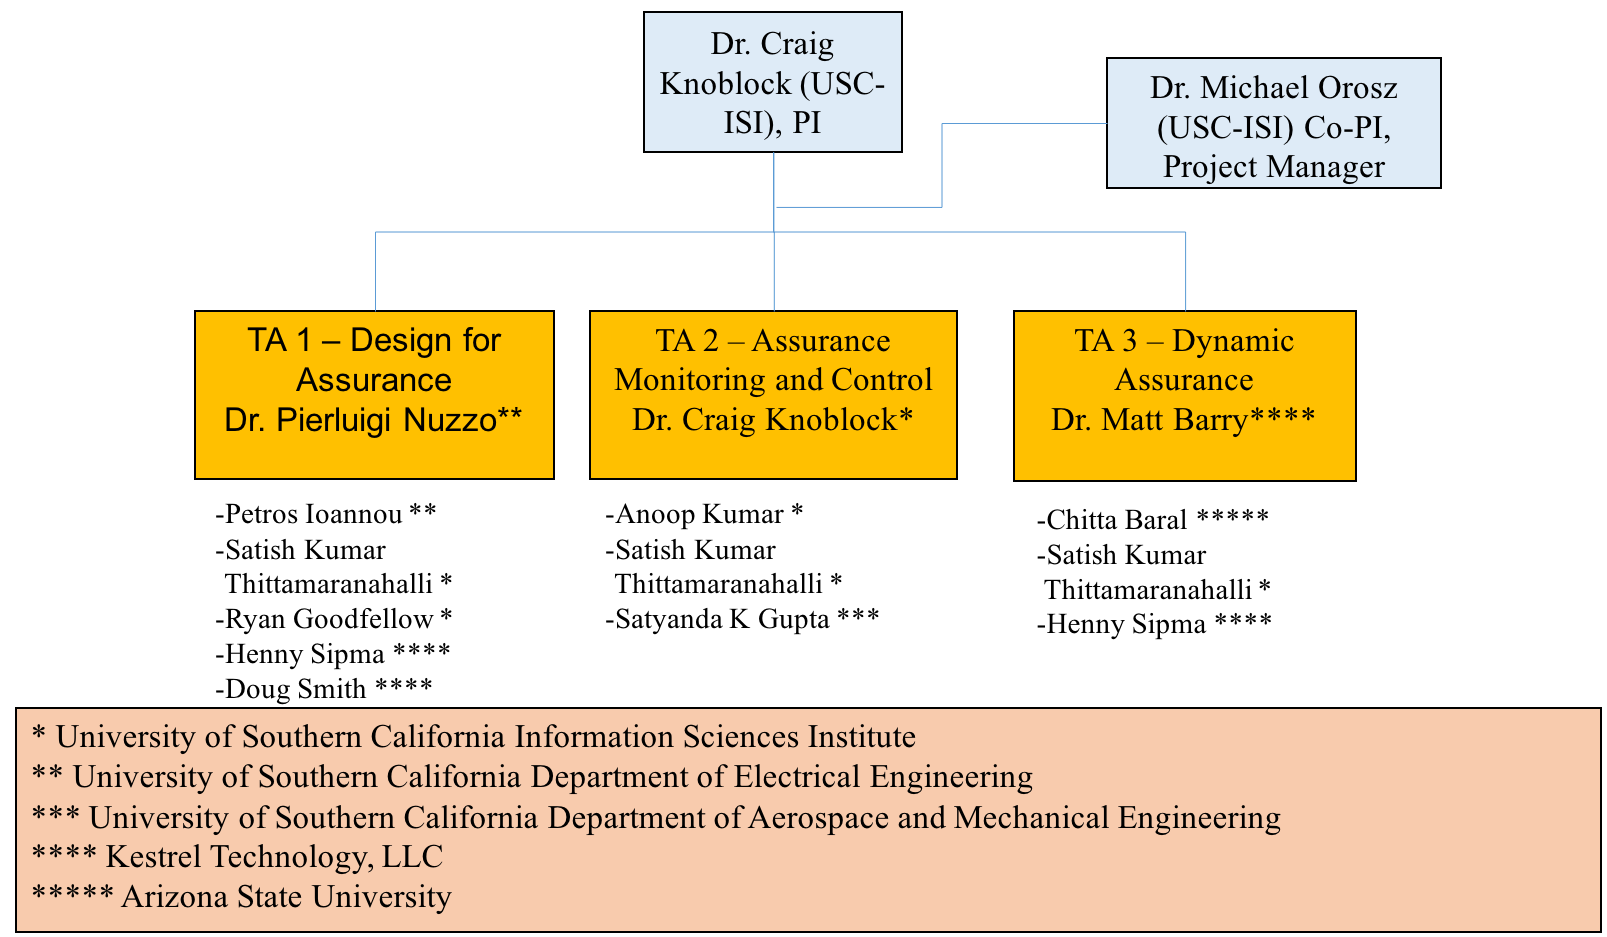
\includegraphics[width=6.0in]{./org-chart2.png}
\caption{\small Organization Chart}
\label{fig:org_chart}
\end{figure}

Coordination: To maximize collaboration and reduce risk to project failure from lack of communication and technical exchange, we plan to employ a wide variety of working styles and communication/coordination so that all can contribute.  At the core of our project will be regularly scheduled meetings bridging the diversely distributed team (Table~\ref{fig:Collaboration_Table}).  These meetings will address project status, identify challenges, implement risk mitigation strategies and participate in technology exchanges and system integration efforts (when appropriate)

\begin{table}[ht]
\caption{\small Project Meetings and Events}
  \centering
  {\footnotesize
\begin{tabular}{|m{3.15in}|m{3in}|} 
\hline
\textbf{Meeting} & \textbf{Frequency} 
\\\hline
Conference calls among investigators (discuss project status, address concerns and project risks) & Weekly
\\
\hline
Technical exchange and coordination meetings using Bluejeans or another videoconference technology & At least twice a month and more frequently as needed
  \\ 
\hline
Face-to-Face meetings (prior to P/I and demonstration meetings) & Every 3 to 6 months and more frequently (especially at the beginning of the project) as needed
 \\\cline{1-2}

\hline
\end{tabular}
}
\label{fig:Collaboration_Table}
\end{table}

\begin{table}[tbhp]
\caption{\small Key Project Team Member Responsibilities}
  \centering
  {\footnotesize
\begin{tabular}{| m{.75in} | m{3.9in}| m{1.5in}|} 
\hline
\textbf{Key Member} & \textbf{Responsibilities} & \textbf{Tasks} 
\\\hline
Dr.\ Craig Knoblock  & Principal Investigator responsible for project, leads TA 2 – Assurance Monitoring and Control.  Will lead the overall project and lead the TA2 team.  Served as the PI on many DARPA projects and has sucessfully led many large teams.    Effort on project:  25\% &
1.1.6, 1.2.2 1.2.3, 1.2.4, 1.3.4, 1.4.1, 
2.1.6, 2.2.2 2.2.3, 2.2.4, 2.3.4, 2.4.1, 
3.1.6, 3.2.2, 3.2.3, 3.2.4, 3.3.4, 3.4.1
\\
\hline
Dr.\ Michael Orosz & Co-Principal Investigator responsible managing the day-to-day operations of the project, assist technical teams as needed, coordinate with TA4 teams.    Has led many large complex multi-disciplined/multi-organizational projects in academic and industry environments.  Effort on project: 50\%
& 1.1.6, 2.1.6, 3.1.6, 1.4.1, 2.4.1, 3.4.1
  \\ 
\hline
Dr.\ Pierluigi Nuzzo 
& 
Co-Principal Investigator.  Leads the TA 1 - Design for Assurance team and conducts research on the formal methods for the design of the TA1 system.  Research experience on methodologies and tools for the design of cyber-physical systems; contracts, interfaces, and compositional methods for embedded system design; the application of automated formal methods and optimization theory to problems in embedded and cyber-physical systems.  Effort on project: 2 months/year (16.6\%)
& 
1.1.1, 2.1.1, 3.1.1 \\
\hline
Dr.\ Matthew Barry
& 
Key personnel.  Leads the TA 3 – Dynamic Assurance.   He will conduct the research on the dynamic assurance case language editors and parsers, the run-time system, and system integrations. Effort on project:  66\%
& 
1.3.2, 2.3.2, 3.3.2\\
\hline
Dr.\ Chitta Baral
& 
Key personnel responsible for learning assurance rules, supporting assurance rules with uncertainty and improving solver speed.  Expertise on ASP solvers, which will be used to reason about the assurance cases. Effort on project: 20\%
& 
1.3.1, 2.3.1, 3.3.1 \\
\hline
Dr.\ Doug Smith 
& 
Key personnel will support formal methods aspects of TA1, and lead the effort on abstract refinement. Expertise in field of automated correct-by-construction program generation.    Effort on project: 40\%
& 
1.1.5, 2.1.5, 3.1.5 \\
\hline
Dr.\ Henny Sipma
& 
Key personnel who will support the program verification tasks under TA1.  Will lead the effort on program verification.   Effort on project:  45\%
& 
1.1.5, 2.1.5, 3.1.5, 1.3.2, 2.3.2, 3.3.2 \\
\hline
Dr.\ Petros Ioannou
& 
Key personnel responsible providing and extending the assurance test bed, which will be available at the start of the project for autonomous vehicles.   Effort on project: 1 month/year (8.3\%)
& 
1.1.2, 2.1.2 (optional), 3.1.2 (optional)
\\
\hline
Dr.\ Satyandra Kumar Gupta
& 
Key Personnel providing autonomous command and control expertise to the TA-2 team.   Will lead the research on safety aware learning on TA2.   Past research on physics-aware decision making to facilitate automation.  Effort on project: 1 month/year (8.3\%)
& 
1.2.1, 2.2.1, 3.2.1 \\
\hline
Dr.\ Anoop Kumar 
& 
Key personnel providing support to the TA 2 project team.  Will lead the research on monitoring \& control and detecting distribution shifts.  Effort on project: 50\%
& 
1.2.1, 1.2.2, 1.2.3, 1.2.4, 2.2.1, 2.2.2, 2.2.3, 2.2.4, 3.2.1, 3.2.2, 3.2.3, 3.2.4\\
\hline
Dr.\ Satish Thittamaranahalli
& 
Key personnel developing scalable algorithms for TA1, TA2, and TA3 project teams.  Has extensive experience on scalable algorithm design, machine learning, and constraint reasoning.  Effort on project: 50\%
& 
1.2.1, 1.2.2, 1.2.3, 1.2.4, 2.2.1, 2.2.2, 2.2.3, 2.2.4, 3.2.1, 3.2.2, 3.2.3, 3.2.4, 1.1.4, 2.1.4, 3.1.4 \\
\hline
Dr.\ Ryan Goodfellow
& 
Key personnel providing support to the TA-1 project. Will lead the research on simulation-based testing.  Has extensive experience on simulation-based testing.  Effort on project:  30\%
& 
1.1.3, 2.1.3, 3.1.3 \\

\cline{1-2}

\hline
\end{tabular}
}
\label{fig:Table_Mgmt}
\end{table}



\newpage
\section{Personnel, Qualifications and Commitment}

{\bf Dr.\ Craig Knoblock}, the PI on this effort, is a Research Professor of both Computer Science and Spatial Sciences at the University of Southern California (USC) and Director of the Intelligent Systems Division at the USC Information Sciences Institute.   He received his Ph.D. from Carnegie Mellon University in computer science. 
%His research focuses on techniques for describing, acquiring, and exploiting the semantics of data.  
In previous projects he has worked on developing  scalable approaches to execution monitoring, accurate detection of sensor failures, and   automatic modeling and reconstruction of sensors.  He has published more than 300 journal articles, book chapters, and conference papers on these topics.  Dr. Knoblock is a Fellow of the Association for the Advancement of Artificial Intelligence (AAAI), a Distinguished Scientist of the Association of Computing Machinery (ACM), a Senior Member of IEEE, past President and Trustee of the International Joint Conference on Artificial Intelligence.
%and winner of the 2014 Robert S. Engelmore Award.  

{\bf Dr.\ Michael Orosz}, a Co-PI on this effort, is a Research Associate Professor of Civil and Environmental Engineering at the University of Southern California (USC) and Research Director of the Decision Systems Group at the USC Information Sciences Institute.  Dr. Orosz has over 30 years’ experience in commercial and government software development, basic and applied research, project management, academic research and has developed and deployed several commercially successful products.  His research interests are in machine learning and decision analytics as applied to intelligence analysis and autonomous command and control such as smart building controls.    Dr. Orosz has extensive experience in managing large complex multi-disciplined/multi-teamed research projects. %funded by DARPA, DHS, DoD, DoE, Industry, NASA, NRO, NSA and ONR.   
He received his Ph.D. in computer science from the University of California, Los Angeles.

{\bf Dr.\ Pierluigi Nuzzo}, a Co-PI on this project, is an Assistant Professor in the Department of Electrical Engineering at the University of Southern California. He received the Ph.D. in Electrical Engineering and Computer Sciences from the University of California at Berkeley. 
%in 2015, and the Laurea degree (MS) in electrical engineering (summa cum laude) from the University of Pisa, Italy, and the Sant'Anna School of Advanced Studies, Pisa, Italy.
%
%He has four years of research experience in analog and mixed signal circuit design as a researcher at IMEC, Leuven, Belgium, and over 10 years experience in design methodologies and tools for mixed-signal integrated circuits and cyber-physical systems, as a researcher at the University of Pisa, IMEC, UC Berkeley, and USC. 
His research interests
include: methodologies and tools for cyber-physical system and mixed-signal
system design; contracts, interfaces and compositional methods for embedded
system design; the application of formal methods and optimization theory to problems in embedded and cyber-physical systems and electronic design automation. 
%
Prof. Nuzzo received %First Place in the operational category and Best Overall
%Submission in the 2006 DAC/ISSCC Design Competition, 
a Marie Curie Fellowship
from the European Union in 2006, 
the University of California at Berkeley EECS
departmental fellowship in 2008, 
%the University of California at Berkeley Outstanding Graduate Student Instructor Award in 2013, 
the IBM Ph.D.
Fellowship in 2012 and 2014, 
%the Best Paper Award from the International Conference on Cyber-Physical Systems (ICCPS) in 2016, 
and the David J.~Sakrison Memorial Prize in 2016 for his doctoral research. 
%He is an author of 1 patent and over 60 publications.

{\bf Dr.\ Satyandra K. Gupta} is Smith International Professor in the Department of Aerospace and Mechanical Engineering at the University of Southern California. %Prior to joining the University of Southern California, he was a Professor in the Department of Mechanical Engineering and the Institute for Systems Research at the University of Maryland. He was the founding director of the Maryland Robotics Center and the Advanced Manufacturing Laboratory at the University of Maryland. 
He served as a program director for the National Robotics Initiative at the National Science Foundation from September 2012 to September 2014.  Dr. Gupta's interest is in the area of physics-aware decision making to facilitate automation. He has published more than 300 technical articles. He is a fellow of the American Society of Mechanical Engineers (ASME) and editor of ASME Journal of Computing and Information Science in Engineering. Dr. Gupta has received the Young Investigator Award from the Office of Naval Research in 2000, CAREER Award from the National Science Foundation in 2001, Presidential Early Career Award for Scientists and Engineers (PECASE) in 2001, Invention of the Year Award at the University of Maryland in 2007, Kos Ishii-Toshiba Award from ASME in 2011, and Excellence in Research Award from ASME in 2013.%, and Distinguished Alumnus Award from Indian Institute of Technology, Roorkee in 2014. %He has also received seven best paper awards at conferences.

{\bf Ryan Goodfellow} is a computer scientist at ISI working in combined cyber physical simulation and emulation platform development. His formal background is in simulation algorithms and modeling techniques using differential-algebraic equations (DAE). He has applied this knowledge in the CPS space by integrating DAE modeling languages and simulation engines with network testbeds to create comprehensive scientific experimentation platforms for cyber-physical systems. These experimentation platforms have been used in the power grid research space. %Ryan is a lead developer on the Deter network testbed, with a strong background in networked and distributed systems engineering. %He is also a combat veteran, serving as a non-commissioned officer and SIGINT team lead for a multi-functional intelligence team in Afghanistan.

{\bf Dr.\ Petros Ioannou} is a Professor in the Department of Electrical Engineering, Director of the Center for Advanced Transportation Technologies and Associate Director for Research for the DOT supported University Transportation Center at USC. He received his MS and PhD from the University of Illinois at Urbana Champaign in Mechanical and Electrical Engineering, respectively. His research interests are in robust adaptive control, vehicle dynamics and control, human factors and safety, automated vehicles, nonlinear systems and Intelligent transportation Systems.  He received the 2016 IEEE Transportation Technologies field award and the 2016 IEEE Control system society Transition to Practice Award. He is a Fellow of IEEE, IFAC and IET and author/coauthor of 8 books and over 400 papers.

{\bf Dr.\ Matthew Barry} will serve as lead for the TA3 tasks. %He will implement the dynamic assurance case language editors and parsers, the run-time system, and system integrations.  He will implement the assurance case arguments and the API for updating argument structure and content.  
Dr. Barry currently is CEO at Kestrel Technology LLC, and previously spent 20 years in NASA space mission operations at the Jet Propulsion Lab and Johnson Space Center.  At NASA Headquarters he led the introduction of dependability case requirements and plans for flight computing systems in upcoming manned space exploration missions, as well as the development of Agency-level software-related safety-critical control system requirements.  He recently served as a Principal Investigator on DHS/Cyber S\&T STAMP (Static Tool Analysis Modernization Program), DARPA CSFV (Crowd Sourced Formal Verification), three NASA Aeronautics R\&D projects, and the AFRL-sponsored Static Analysis of Numerical Algorithms project.  Dr. Barry earned BSME, MS, and PhD degrees in mechanical engineering, and an MBA degree, from Rice University.  

{\bf Dr.\ Henny Sipma} will support the program verification tasks under TA1.  %She is the key person behind the company's {\em KT Advance\/} and {\em KT Transferal\/} static analysis products, and the designer and programmer of the company's core {\em CodeHawk\/} abstract interpretation engine. 
Dr. Sipma currently is the CTO at Kestrel Technology LLC.  She has spent the past 10 years with Kestrel Technology as a static analysis expert; previously developed and taught static analysis techniques as senior research associate at Stanford University for eight years; and developed industrial process controls as an senior systems analyst at Shell.  She has been Principal Investigator or company lead on several recent R\&D projects for Federal agencies, including two projects under the IARPA STONESOUP (Securely Taking On New Executable Software of Uncertain Provenance) program; the DHS Cyber S\&T Gold Standard project; and the DARPA-sponsored STAC (Space-Time Analysis for Cybersecurity) and MUSE (Mining and Understanding Software Enclaves) programs.  Dr. Sipma earned 
%a BS degree in chemistry and an MS degree in chemical engineering at the University of Groningen in The Netherlands, and 
MS and PhD degrees in computer science from Stanford University.  

{\bf Dr.\ Douglas R.\ Smith} will support formal methods aspects of TA1, including the enforcement of safety properties and the generation of monitors.  He is President of Kestrel Technology LLC and Principal Scientist at Kestrel Institute.  He is a Fellow of the American Association of Artificial Intelligence (AAAI) and an ASE Fellow (Automated Software Engineering).  From 1986 to 2000, he taught an advanced graduate course on correct-by-construction software development at Stanford.  
%Dr. Smith has led the development of a series of software synthesis systems, including KIDS (Kestrel Interactive Development System), Specware, Designware, and Planware. 
%Applications domains have included a variety of complex high-performance planners and schedulers for the US Air Force.  He leads current projects on the generation of air mission plans and cyberoperations.  
Other recent projects focused on automated policy enforcement \cite{SmithD0703,SmithD08}, synthesis of secure network protocol codes, and the synthesis of high-performance constraint-solvers\cite{SmithD08c,SmithD13}.  Dr. Smith has over 30 years experience in the field of automated correct-by-construction program generation and has published over 100 papers. He has one patent.  He received the Ph.D. in Computer Science from Duke University% in 1979.  

{\bf Dr. Chitta Baral} is a Professor in the Department of Computer Science and Engineering at Arizona State University. He will support the TA3 efforts on Learning assurance rules, supporting assurance rules with uncertainty and improving solver speed. Dr. Baral has expertise in various aspects of autonomy and Artificial Intelligence. 
He wrote the first book on answer set programming (published by Cambridge University Press) the formal language behind our assurance rules. Some of his other works relevant to this proposal are: goal specification for autonomous systems, automatic construction of control rules for autonomous systems that satisfy given goals, combining machine learning with reasoning in various contexts, including image understanding. %He is the President of KR Inc. He is an associate editor of AIJ and has been an associate editor of JAIR.

{\bf Dr.\ Satish Kumar Thittamaranahalli (T. K. Satish Kumar)} leads the Collaboratory for Algorithmic Techniques and Artificial Intelligence (CATAI) at USC's Information Sciences Institute. He has published over 60 papers on numerous topics in Artificial Intelligence spanning such diverse areas as Constraint Reasoning, Planning and Scheduling, Probabilistic Reasoning, Robotics, Combinatorial Optimization, Approximation and Randomization, Heuristic Search, Model-Based Reasoning, Knowledge Representation and Spatio-Temporal Reasoning. %He %has served on the Program Committees of many international conferences in Artificial Intelligence
He and is a winner of the 2016 Best Robotics Paper Award and the 2005 Best Student Paper Award from the International Conference on Automated Planning and Scheduling. 
Dr. Kumar received his PhD in Computer Science from Stanford University. %In the past, he has also been a Visiting Student at the NASA Ames Research Center, a Postdoctoral Research Scholar at the University of California, Berkeley, a Research Scientist at the Institute for Human and Machine Cognition, a Visiting Assistant Professor at the University of West Florida, and a Senior Research and Development Scientist at Mission Critical Technologies.

\textbf{Dr.\ Anoop Kumar} is a senior computer scientist at USC ISI and has broad expertise in machine learning, statistical modeling, and software engineering.  Dr.\ Kumar is the technical lead on the DARPA RSPACE program and has played a vital role in developing a system that fuses air operations data from multiple sources, maintains world state, and issues warnings. Previously, he led the research and development of the BBN’s election forecasting system for the IARPA OSI program. %Dr.\ Kumar played a significant role in the DARPA DEFT program by developing a model to support integration of output from multiple NLP algorithms. He has contributed at the development to management levels on government research contracts and commercial projects. 
Dr.\ Kumar helped design and develop BBN's commercially available, hosted speech and medical transcription services offering. 

\begin{table}[!tbh]
\begin{footnotesize}
\vspace{-0.1in}

\begin{tabular}{lll}
\begin{tabular}[t]{|l|@{}c@{}|@{}c@{}|@{}c@{}|@{}c@{}|} \hline
Project & Status & \multicolumn{3}{ c| }{Hours} \\ \cline{3-5}
& & P1 & P2 & P3 \\ \hline



\multicolumn{5}{ |c| }{ \textbf{Craig Knoblock} } \\ \cline{1-5}
Safeguard & Pro & 770 & 641 & 641 \\ \cline{1-5}
ELICIT & Cur & 308 & 256 & 120 \\ \cline{1-5}
WTNIC & Cur & 11 & 0 & 0 \\ \cline{1-5}
EFFECT & Cur & 641 & 107 & 0 \\ \cline{1-5}
LinkedMaps & Cur & 203 & 25 & 0 \\ \cline{1-5}
PRINCESS & Cur & 608 & 96 & 0 \\ \cline{1-5}
SCHARP & Cur & 481 & 54 & 0 \\ \cline{1-5}
MINT & Pen & 650 & 534 & 285 \\ \cline{1-5}

\multicolumn{5}{ |c| }{ \textbf{Michael Orosz} } \\ \cline{1-5}
Safeguard & Pro & 1560 & 1300 & 1300  \\ \cline{1-5}
SMC/SY & Cur & 1803 & 0 & 0  \\ \cline{1-5}

\multicolumn{5}{ |c| }{ \textbf{Matthew Barry} } \\ \cline{1-5}
Safeguard & Pro & 2078 & 1690 & 1554 \\ \cline{1-5}
Starlite & Cur & 1840 & 1692 & 0 \\ \cline{1-5}



\multicolumn{5}{ |c| }{ \textbf{Anoop Kumar} } \\ \cline{1-5}
Safeguard & Pro & 1560 & 1300 & 1300 \\ \cline{1-5}

\end{tabular}
&
\begin{tabular}[t]{|l|@{}c@{}|@{}c@{}|@{}c@{}|@{}c@{}|} \hline
Project & Status & \multicolumn{3}{ c| }{Hours} \\ \cline{3-5}
& & P1 & P2 & P3 \\ \hline

\multicolumn{5}{ |c| }{ \textbf{Pierluigi Nuzzo} } \\ \cline{1-5}
Safeguard & Pro & 520 & 433 & 433  \\ \cline{1-5}
Mirage & Cur & 433 & 0 & 0  \\ \cline{1-5}

\multicolumn{5}{ |c| }{ \textbf{Satyandra Gupta} } \\ \cline{1-5}
Safeguard & Pro & 260 & 217 & 217 \\ \cline{1-5}
Human   & Cur & 22 & 0 & 0 \\ \cline{1-5}
Vehicles & Cur & 36 & 0 & 0 \\ \cline{1-5}
Robot & Cur & 116 & 0 & 0 \\ \cline{1-5}
Assembly & Cur & 33 & 0 & 0 \\ \cline{1-5}
Solar & Cur & 4 & 0 & 0 \\ \cline{1-5}

\multicolumn{5}{ |c| }{ \textbf{Petros Ioannou} } \\ \cline{1-5}
Safeguard & Pro & 260 & 217 & 217 \\ \cline{1-5}
CPS & Cur & 130 & 0 & 0 \\ \cline{1-5}

\multicolumn{5}{ |c| }{ \textbf{Ryan Goodfellow} } \\ \cline{1-5}
Safeguard & Pro & 936 & 780 & 780 \\ \cline{1-5}
STEAM & Cur & 416 & 0 & 0 \\ \cline{1-5}


\end{tabular}
&
\begin{tabular}[t]{|l|@{}c@{}|@{}c@{}|@{}c@{}|@{}c@{}|} \hline
Project & Status & \multicolumn{3}{ c| }{Hours} \\ \cline{3-5}
& & P1 & P2 & P3 \\ \hline

\multicolumn{5}{ |c| }{ \textbf{Chitta Baral} } \\ \cline{1-5}
Safeguard & Pro & 659 & 485 & 485 \\ \cline{1-5}
PostdocBP & Cur & 176 & 0 & 0 \\ \cline{1-5}
Languages & Pen & 528 & 264 & 264 \\ \cline{1-5}
CAREER & Pen & 88 & 44 & 44 \\ \cline{1-5}
CHS & Pen & 510 & 255 & 0 \\ \cline{1-5}

\multicolumn{5}{ |c| }{ \textbf{Doug Smith} } \\ \cline{1-5}
Safeguard & Pro & 1222 & 984 & 840 \\ \cline{1-5}
RSPACE & Cur & 342 & 0 & 0 \\ 
\cline{1-5}
PLANX & Cur & 154 & 0 & 0 \\ 
\cline{1-5}
HACCS & Pen & 923 & 769 & 769 \\ 
\cline{1-5}

\multicolumn{5}{ |c| }{ \textbf{Henny Sipma} } \\ \cline{1-5}
Safeguard & Pro & 1372 & 962 & 840 \\ \cline{1-5}
STAC & Cur & 797 & 0 & 0 \\ \cline{1-5}

\multicolumn{5}{ |c| }{ \textbf{Satish Thittamaranahalli} } \\ \cline{1-5}
Safeguard & Pro & 1560 & 1300 & 1300 \\ \cline{1-5}
MapF & Cur & 103 & 103 & 0 \\ \cline{1-5}

\end{tabular}
\end{tabular}

\end{footnotesize}
\caption{Individual commitments of key personnel}
\label{tab:Commitments}
\vspace{-0.2in}
\end{table}

\clearpage
\newpage
\section{Capabilities}


%\subsection{University of Southern California}
USC has strengths in number of areas that are closely related to the proposed work:
\begin{itemize}[itemsep=0pt,leftmargin=*]
\item Dr.\ Nuzzo 
%has over 10-year research experience in embedded system design, from mixed-signal chip design (analog-to-digital converters, frequency synthesizers, software-defined radio), to methodologies and tools for mixed-signal integrated circuits and Cyber-Physical Systems (CPSs), and the application of formal methods and optimization theory to problems in embedded and cyber-physical systems and electronic design automation.  
%His doctoral work 
has done extensive research on contracts and compositional methods for heterogeneous system design and design space exploration, with application to aircraft electric power systems and environmental control systems. His work has helped transition rigorous system design foundations, innovative design methodologies, and new systems engineering paradigms to industry (IBM, United Technologies). 
\item Dr.\ Satyandra K. Gupta has worked on autonomous surface vehicles, autonomous ground vehicles for operation on rugged terrains, and autonomous flapping wing aerial vehicles.   His group has developed a hierarchal decision making approach for realizing autonomous systems. 
%This approach combines task planning and assignment, deliberative trajectory planning, reactive collision avoidance behaviors, and trajectory tracking control layers. 
His group has also developed new methods for learning reactive behaviors in adversarial environments and COLREGS compliant trajectory planning. \item Dr.\ Knoblock has developed methods that learn the relationships between sensors to both identify failures and changes in sensor and reconstruct those sensors, providing estimates of the accuracy of the reconstructed sensors.  
\item Ryan Goodfellow has extensive experience in simulation based testing through high-fidelity CPS testbed environment development and operation, using the Deter network testbed as the core which has supported several large scale government projects from a variety of agencies and thousands of users. %we have developed sophisticated CPS experiments under programs such as NFS RIPS, NIST SmartCities and the DHS Cybersecurity showcase.
\item Dr.\ Ioannou %helped  design and implement adaptive cruise control systems in collaboration with Ford Motor Company, which was commercialized four years before any other company. He 
worked on several DOT funded projects on automated vehicles and intelligent highway systems where he demonstrated his vehicle control designs for safety and performance on actual automated vehicles in test trucks and I-15 highway.
\item Drs.\ Knoblock, Kumar, and Thittamaranahalli have developed highly scalable approaches for monitoring message traffic to identify potential problems and issue warnings and alerts. 
\item Dr. Thittamaranahalli has developed state-of-the-art methods for efficiently solving large-scale search and optimization problems. %These techniques will be applicable in TA2 for safety-aware learning and planning, in TA2 for assurance monitoring and control, and in TA3 for dynamic assessment of assurance cases.

\end{itemize}
%\subsection{Kestrel Technology LLC}

Kestrel Technology's strength is in program analysis, specifically static analysis of both source and binary targets.  The company performs applied R\&D and product development for a variety of static analysis applications  pivoting primarily on the abstract interpretation technique.  The company recently initiated development of program analysis applications using logical equivalence techniques. As a provider of verification evidence in the form of mathematical proofs, the company also has expertise in the design and development of assurance case arguments for high-integrity systems using such evidence. %The company is engaged in a partnership with Wind River Systems to develop program analysis tools for its embedded system developers.  Many of Wind River's customers must develop their products under safety and certification standards, including those using safety cases.  

   

%\subsection{Arizona State University}
Chitta Baral at Arizona State University has developed various software to learn assurance rules and various ASP solvers, which he has made available as open-source.

Most of the software carried forward for implementation or derivation is open source.  The single exception is Kestrel Technology's {\it KT Advance\/} static analysis tool (TA1), in particular the abstract interpretation engine therein, which is company proprietary and is US EAR export-controlled.   
%Owing to mixed funding for the development of that technology 
We will continue to provide the Federal government a restricted use license for that particular item.

There are no specialized facilities, data, or GFE required for this effort. 

\include{sow}
\include{milestones}

% \section{Level of Effort by Task \textcolor{red}{[Mike/Lisa - 1 pages]}}

% \textcolor{blue}{
% \begin{itemize}
% \item Will be a separate spreadsheet
% \item
% \end{itemize}
% }

\include{appendix_a}

%\section{Appendix B \textcolor{red}{[No Page Count]}}

\section{References}
\bibliographystyle{acm} 
\bibliography{TA3/ta3,TA2/ta2,TA1/ta1}
\end{document}
%%\documentclass[a4paper]{article}
%\documentclass[12pt]{article}
\documentclass[12pt]{dod-blank}

%% Language and font encodings
\usepackage[english]{babel}
\usepackage[utf8x]{inputenc}
\usepackage[T1]{fontenc}

%% Sets page size and margins
%%\usepackage[a4paper,top=3cm,bottom=2cm,left=3cm,right=3cm,marginparwidth=1.75cm]{geometry}
%\usepackage[top=1in, bottom=1in, left=1in, right=1in]{geometry}



%% Useful packages
\usepackage{amsmath}
\usepackage{graphicx}
  \graphicspath{{.}{./image/}}
  \DeclareGraphicsExtensions{.png,.jpg} 
\usepackage[colorinlistoftodos]{todonotes}
\usepackage[colorlinks=true, allcolors=blue]{hyperref}
\usepackage{tabularx}
\usepackage{multirow}
\usepackage{tabulary}
\usepackage{float}
\usepackage{wrapfig}
\usepackage[export]{adjustbox}
\usepackage{comment}
\usepackage{tabularx}
\usepackage{multirow}
\usepackage{tabulary}
\usepackage{enumitem}

\usepackage{listings}
\usepackage{color}
\usepackage{array}
\usepackage{subcaption}
\usepackage{xcolor}




\renewcommand{\textfraction}{0}
\renewcommand{\topfraction}{1.0}
\renewcommand{\bottomfraction}{1.0}

\usepackage{longtable}
%% macros
\newif\iffinal
\finaltrue
\iffinal
  
    \newcommand\baareq[1]{}
    \newcommand\baades[1]{}
 
 
\else
    \definecolor{darkgreen}{rgb}{0,0.4,0}
    \definecolor{darkcyan}{rgb}{0,0.4,0.4}
    \definecolor{darkblue}{rgb}{0,0,0.5}
    
    \newcommand\baareq[1]{{\color{darkcyan}[\textbf{Requirement:} #1]}}
    \newcommand\baades[1]{{\color{darkcyan}[\textbf{Description:} #1]}}
 
\fi




\def\naive{na\"{\i}ve}



\lstset{ 
  backgroundcolor=\color{white},   % choose the background color; you must add \usepackage{color} or \usepackage{xcolor}
  basicstyle=\footnotesize\ttfamily,            % the size of the fonts that are used for the code
  breakatwhitespace=false,         % sets if automatic breaks should only happen at whitespace
  breaklines=true,                 % sets automatic line breaking
  captionpos=b,                    % sets the caption-position to bottom
  commentstyle=\color{mygreen},    % comment style
  % deletekeywords={...},            % if you want to delete keywords from the given language
  escapeinside={\%*}{*)},          % if you want to add LaTeX within your code
  extendedchars=true,              % lets you use non-ASCII characters; for 8-bits encodings only, does not work with UTF-8
  frame=single,	                   % adds a frame around the code
  keepspaces=false,                 % keeps spaces in text, useful for keeping indentation of code (possibly needs columns=flexible)
  keywordstyle=\color{blue}\bfseries\underbar,       % keyword style
  language=Prolog,                 % the language of the code
  % morekeywords={if,and},        % if you want to add more keywords to the set
  numbers=none,                    % where to put the line-numbers; possible values are (none, left, right)
  numbersep=5pt,                   % how far the line-numbers are from the code
  numberstyle=\tiny\color{mygray}, % the style that is used for the line-numbers
  rulecolor=\color{black},         % if not set, the frame-color may be changed on line-breaks within not-black text
  showspaces=false,                % show spaces everywhere adding particular underscores; it overrides 'showstringspaces'
  showstringspaces=false,          % underline spaces within strings only
  showtabs=false,                  % show tabs within strings adding particular underscores
  stepnumber=2,                    % the step between two line-numbers. If it's 1, each line will be numbered
  stringstyle=\color{mymauve},     % string literal style
  tabsize=2,	                   % sets default tabsize to 2 spaces
  title=\lstname                   % show the filename of files included with \lstinputlisting; also try caption instead of title
}

% apply trick for additional keywords for our AC DSL
\lstset{
	emph={for, if, and, or},
    emphstyle={\color{blue}\bfseries\underbar}
}




\title{DARPA Assured Autonomy}
\author{Technical Volume- \textcolor{red}{Thirty-Eight (38) pages max}}

\begin{document}
\pagenumbering{roman}
\include{cover}

\newpage
\section{Table of Contents}
\tableofcontents

\newpage
\pagenumbering{arabic}
\section{Executive Summary}
As we rapidly move into a world where machine learning plays a central role in realizing autonomous systems, it is becoming increasingly important to develop techniques that assure that these systems will operate safely and perform as expected. Current approaches are limited to providing assurance for systems with limited or no  learning capabilities. In this context, DARPA's Assured Autonomy BAA seeks to \emph{develop rigorous design and analysis technologies for continual assurance of learning-enabled autonomous systems}. USC in collaboration with Kestrel Technology and ASU is pleased to submit a comprehensive TA1, TA2, and TA3 proposal entitled \emph{``Assured Autonomy for Learning Enabled Vehicles (Safeguard).''} We plan to provide an end-to-end solution to support autonomous systems with learning-enabled components, ranging from design technologies for assurance, to assurance monitoring and control techniques, to representation and online evaluation of assurance cases. We have assembled a strong team of experts that cover the range of technologies that are required to create such an end-to-end system. If successful, the project will provide the technologies for building the next-generation of learning-enabled autonomous systems.  The entire project will take four years and cost \textcolor{red}{\$??}, with an initial version completed at the end of Phase I and successive versions with additional capabilities and improved scalability at the end of Phase II and Phase III.  

In the remainder of this section, we first introduce an  unmanned surface vehicle scenario that will be used throughout the proposal to describe the approach.  Next, we describe our approach to design, monitoring, and dynamic assurance. Finally, we introduce the team involved in the project. 

\textbf{Motivating Scenario.} Consider an autonomous unmanned surface vehicle (USV) guarding a valuable asset in the ocean when an unknown vehicle  approaches the security perimeter, under challenging weather conditions. In this scenario, the USV is required to approach the intruding vehicle, issue a warning signal, and escort it to a safe distance from the controlled area. However, as the USV has no a priori knowledge of its external environment behaviors (e.g., water depth, waves, wind, current, visibility), pre-computing a feasible trajectory, let alone optimal, becomes a non-trivial problem. For trajectory planning, the USV must continuously perform the following tasks:
\begin{itemize}[itemsep=0pt,leftmargin=*]
 \item Sense the current state of the surrounding environment (e.g., water depth, waves, wind, current, visibility) and estimate its own maneuverability constraints (e.g., braking distance, available acceleration, maximum velocity, turning radius, turning rate, safety distance) based on the state of the environment;      
\item Sense the static obstacles in the sensor range and generate a traversability map;
\item Sense the moving obstacles and classify them;   
\item Predict future trajectories of moving obstacles; 
\item Determine if any of the COLREGS \cite{commandant1999international} rules will be in effect with respect to one or more of the nearby vessels and identify the vessels with the right of way.    
\end{itemize}
The above information will be used by the trajectory planner to compute an initial trajectory, which will be continuously refined as the USV gathers additional information.
% It is not possible for the USV to be tested in every possible environment. 
The USV will use learning enabled components to take  decisions as it encounters new situations, such as  
\begin{itemize}[itemsep=0pt,leftmargin=*]
\item Classifiers to identify moving obstacles based on physical appearance and motion signatures,
\item Algorithms to estimate the sensor capabilities in adverse weather conditions,   
\item Algorithms to accurately estimate uncertainty in the environment, 
\item Classifiers to generate traversability maps,
\item Prediction of external vessel behaviors based on motion histories, 
\item Reinforcement learning  to ensure COLREGS compliance of maneuvers,  
\item Algorithms to learning pursuit behaviors.  
\end{itemize}
Learning enabled components will interact with each other in complex ways, where a misclassification error in one component may eventually compromise the entire mission.   
% We will need to make sure that each learning enabled components has a run-time monitor that will ensure that the assumptions made by the learning-enabled component remain valid and prevent erroneous learning. 
% For example, if the vehicle is exhibiting significant error in trajectory tracking, then simply downgrading the trajectory tracking error value may not be a good option.  The failure of prediction of trajectory tracking error might be due to the presence of a significant wake caused by a nearby vessel. The presence of the nearby vessel can be used to explain the degradation in trajectory tracking performance. As the vessel moves away, we can expect the trajectory tracking performance to return to the predicted level.  
While exhaustive validation of learning-enabled cyber-physical systems (LE-CPSs) is a prohibitive task~\cite{Kalra16},
their complexity, heterogeneity, and highly dynamic nature
make it challenging to even leverage existing model-based development techniques to effectively assess system correctness 
% dependability, 
at design time or enforce it at runtime.

\textbf{Design for Assurance.} Safeguard uses a platform-based design approach~\cite{Nuzzo15b} to organize the design process for a LE-CPS and to build assurance cases. Composite models are developed at several levels of abstraction,
from top-level system requirements and safety constraints down to the
implementation level.  Intermediate levels add detail to the levels
above.  The different levels are connected by refinement mappings that
allow properties established at one level to be preserved at the next
level (see Figures~\ref{fig:methodology} and~\ref{fig:assurance}).

Contracts are used to formally specify components and composite models
in terms of (1) Assumptions -- the assumed behaviors of the
environment and the behaviors of other components, and (2) Guarantees
-- the behavior properties that a model guarantees if it operates in a
context that satisfies its assumptions.  A calculus of contracts
allows horizontal composition of contracts to generate contracts for
composite models.  Vertical contracts are used to specify the mapping
or refinement relation between models at different levels of
abstraction.  The system design process starts with a high-level
contract that expresses overall system assumptions and requirements.
Subsequent levels express models with increasing detail until the
lowest level expresses the system in terms of hardware components and
their software controllers.

The assurance case for a CPS arises from the horizontal and vertical
structure of the design in several ways.  The components used within a
particular level are either (1) synthesized using
correct-by-construction design tools together with proofs, (2) derived
statically or dynamically using safety-aware machine-learning
techniques, (3) written manually and verified by analysis tools, or
(4) written manually and validated by extensive testing.  The
assurance case for the whole reflects its compositional structure.  We
anticipate that well-specified contracts together with the calculus of
contracts will eliminate well-known problems with unexpected emergent
behaviors in CPS systems.

The assurance case for the lowest-layer design arises from both the
intra-level assurance and from properties and their proofs that are
preserved under the refinement mapping from the top-level
requirements.  The refinement mappings between model layers will be
constructed using a variety of techniques.  A contract at an abstract
level can be mapped to a component or refined contract by (1)
retrieval of pre-verified components from a platform library, (2)
synthesis using correct-by-construction design and optimization tools,
or (3) manual coding to satisfy a contract.  The mapping of a
composite model will be composed from the mappings of its constituent
components or contracts.  When a composite model cannot be mapped
compositionally to the next level, it will be generated using
correct-by-construction design and optimization tools.

\textbf{Assurance Monitoring and Control.}
We provide an integrated framework for safety-aware learning, assurance monitoring and control, detecting distribution shifts. Three major components offer an efficient TA2 architecture as well as interfaces with TA1 and TA3, that is, (a) safety-aware learning and planning, (b) assurance monitors for guarding architectural and safety constraints; and (c) distribution shift detection.

We will develop a new learning-enabled online decision-making framework that allows opportunistically composing a sequence of actions (maneuvers) to reduce uncertainty in the system capability model without suspending the progress toward the mission goals or compromising safety. Each candidate action is evaluated based on three criteria: (1) the risk of violating a safety constraint using the current uncertainties in the parameter estimates; (2) its relevance to the mission goals; (3)  its expected information gain, i.e., reduction in uncertainty, with respect to the parameter estimates. These evaluations are combined to produce a cumulative mission utility value for each action that drives our learning-enabled decision-making framework. The problem of generating and evaluating sequences of actions can be posed in several way. For example, it can be solved using a branch-and-bound search method like Anytime A*, or formulated with the finite-horizon Markov Decision Process (MDP) framework. We will develop new scalable search strategies to solve this problem efficiently, by potentially evaluating a recent method developed at USC, called FastMap, that can significantly improve the execution time. 

We will develop monitors for architectural and safety constraints. 
% While these constraints can be checked over and over again as sensor information flow in, this naive strategy accounts for a lot of computational overhead. 
To achieve scalability and decrease the overhead, we propose the application of a technique that we currently use in DARPA's RSPACE program, which leverages a physical model of the vehicles dynamics and its interactions with the environment to efficiently determine the readout frequency. We propose two  extensions of this basic idea. First, we will use the theory of Variable Elimination to prioritize which variables to monitor, e.g., controllable, versus uncontrollable, adversarially controlled, or unobservable variables. Second, we invoke the dynamic assessment of assurance cases only when needed. This  decreases the number of times dynamic assessment of assurance cases is initiated as well as the communication bandwidth between the TA2 and TA3 components.

Finally, we will identify a distribution shift by combining statistical and machine learning techniques to differentiate between environmental and sensor changes. We will exploit a categorization of the shifts based on their cause and duration as well as extend our earlier work on detecting and mitigating sensor failures for all types of monitored variables.  

\textbf{Dynamic Assurance:} The Safeguard {\em design for assurance\/} activity takes a systems-theoretic stance toward safety.  Consequently, it presumes that safety is an emergent property of the system, and that hazards can present themselves through unintended interactions and performance violations in addition to causal events such as component failures.  Our design approach includes consideration of intent as well as hazard analysis and mitigation.  The artifacts from these activities populate contracts and assumptions for the dynamic assurance case.  
We thus build safety into the product by working at a systems-level viewpoint, using lexicon and design patterns familiar to both hardware and software engineers; safety is an emergent property of the system, not an afterthought.  
As system behavior evolves during runtime owing to learning, threats, degradation, or some other factor, the dynamic assurance case identifies whether the safety constraints continue to be satisfied.  If not, it provides notifications or issues recovery instructions directly from a lookup table.

Our implementation of the dynamic assurance case employs a declarative knowledge base inference engine and a domain-specific language tailored to our approach.  We have used them successfully for assurance case tool sets and arguments, and will extend them to reason about uncertainty and learning.  Our approach to achieve scalability is to specialize solvers toward modularity and to take advantage of domain knowledge.  Specifically, we will develop answer set programming techniques for context-dependent learning for reasoning about the learning-enabled components as well as learning assurance rules.  We will develop new formalisms for uncertainty to include causality, using weights for computing probabilities, and probabilistic non-monotonicity.  To achieve scaling objectives we will implement specializations using modularity, weighted CSPs, and message passing. 

% The system safety constraints revealed from that design become the key elements of our dynamic assurance case.  Our verification tools ensure the constraints are relevant, identifiable, and their implementation and effect observable.  

\textbf{Team.} We have assembled a team that is exceptionally well-qualified to build the proposed Safeguard system.  The team will be led by Dr.\ Craig Knoblock, the Principal Investigator for the effort, who currently leads the Intelligent Systems Division at the Information Sciences Institute.  He has led many large DARPA and IARPA projects over the years and has a strong track record in conducting leading edge research and then transitioning the technology to commercial use.  He will be supported by Dr.\ Michael Orosz as the Project Manager, who also has  experience in managing large research projects and on autonomous systems.  The TA1 team will be led by Dr.\ Pierluigi Nuzzo, who is an expert in embedded system design methodologies and the  application of formal methods to cyber-physical systems.  The TA1 team also includes Dr.\ Doug Smith, who has spent many years working on scalable correct-by-construction techniques and Dr.\ Henny Sipma, who has significant experience in applying program verification methods to real-world problems.  The TA1 team also includes Ryan Goodfellow, who has done a large amount of work on simulation-based testing.  The TA2 team will be led by Dr.\ Knoblock who has worked on topics related to both monitoring and detecting distribution changes.  He will be supported by Dr.\ Satyandra Gupta, who is an expert on autonomous surface vehicles as well as on safety-aware learning. He will also be supported by Drs.\ Anoop Kumar and Satish Thittamaranahalli, who have also previously worked on efficient methods for execution monitoring.  The TA3 team will be lead by Dr.\ Matthew Barry, who has experience in creating the technologies for assurance cases.  He will be supported by Dr.\ Chitta Baral, who is an expert on ASP solvers and by Dr.\ Thittamaranahalli who is an expert on SAT solvers, both of which will be applied to provide scalable assurance case reasoning.  Finally, Dr.\ Petros Ioannou, who is an expert on control systems for autonomous vehicles will provide an autonomous vehicle platform, which will form the focus of our work until the TA4 teams provide additional vehicle platforms for development.  

\newpage
\section{Innovative Claims and Deliverables}

In this project we will develop and build an end-to-end system for assured autonomy.  This section describes the key innovations by technical area and then the overall deliverables of the project.

\paragraph{Design for Assurance}

\begin{itemize}[itemsep=0pt,leftmargin=*]
\item We address the LE-CPS design challenges via a holistic approach that can contextually generate design artifacts and assurance cases. We develop a compositional, contract-based modeling framework, methods, and tools to support the design process from system-level requirement capture,  formalization, and analysis, to the generation, testing, and continual monitoring of software and hardware artifacts in feedback loop with a physical process.

\item We develop compositional abstractions and interfaces (vertical contracts) that can  bridge heterogeneous formalisms and heterogeneous decomposition architectures to make system analysis and synthesis tractable, consistently combine different verification and synthesis methods at design time, and provide seamless support for dynamic assurance at run time. %We aim to quantitatively capture the confidence in the satisfaction of requirements under uncertain or unknown conditions, and resilience properties of  systems at different abstraction levels, to enable trade-off evaluation between resilience, performance, and cost.

\item We develop a unifying framework and efficient algorithms to reason about the combination of discrete and continuous dynamics and constraints in the presence of uncertainties in LE-CPS using a satisfiability modulo convex approach~\cite{Shoukry2017} for contract-based system verification and scalable trajectory planning.  

\item We provide an environment for high-fidelity CPS testing, in which production-ready software, e.g.,  safety-critical learning and control, may be deployed and tested 
% by extending the Cypress testbed environment \cite{Goodfellow2015Cypress:Systems} 
with time dilation facilities, so that it synchronizes with a physical simulation that is not necessarily running in real time, while still having the perception of real time.

\item We 
% These facilities allow a cyber system to be  
propose an approach for unanticipated behavior space identification and test coverage maximization which leverages results from the theory of differential algebraic equation (DAE)~\cite{Berger2013ControllabilitySurvey,Ilchmann2005ATheory,BergerOnSystems,Lamour2013} 
to prune the behavior search space and identify smaller regions of interest for efficient simulation-based testing. 
% We then compute the intersection of these two behavior spaces and restrict our simulation based testing search space to this subspace.
\end{itemize}

\paragraph{Assurance Monitoring and Control}

\begin{itemize}[itemsep=0pt,leftmargin=*]
\item 
%We integrate safety-aware learning into the overall decision making problem. The goal is to maximize mission utility without violating the safety constraints. 
Our safety-aware learning framework enables the system to opportunistically select and execute actions to assist the learning-enabled component in reducing model uncertainty without compromising safety or deviating from the mission goals. The value of uncertainty reduction is explicitly incorporated in the optimization process for selecting the best action.  
\item For safety-aware learning, we propose the idea of preprocessing the search space of the problem domain before queries and observations come in. With such a linear-time preprocessing phase, the performance of search and optimization algorithms can be significantly boosted. For example, in regular A* search, the intensional or extensional search space can be preprocessed in near-linear time to yield an embedding of each state as a point in Euclidean space~\cite{cujakk}. Then, when the query comes in, A* search can make use of these Euclidean distances as heuristic distances between two states to yield order-of-magnitude speedups. 
%In Anytime A* for safety-aware learning and planning, this leads to a significantly better quality of actions chosen within a time limit, and in the MDP framework, the same ideas can be used to improve the convergence of Bellman updates for safety-aware Reinforcement Learning.
\item As massive amounts of sensor information flow in, it is imperative for us to efficiently process this information for monitoring architectural and safety constraints. Building on our past work on similar tasks, we propose novel technologies for efficiently monitoring constraints. These algorithms can yield an exponential reduction in the amount of sensor data that needs to be processed. Doing this also reduces the message complexities between the various modules. %We also propose to use the theory of Variable Elimination (VE) to monitor constraints with uncontrollable, adversarially controlled, and/or unobservable variables. VE yields a substrate constraint to monitor that characterizes a dominant strategy of the controllable variables over the uncontrollable, adversarially controlled, and/or unobservable variables.
\item We will develop techniques to identify  distributional shifts and determine the underlying cause (e.g., change in environment, sensor failure,   etc.), as well as strategies for handling the various distributional shifts.   Notably, we propose to build on our past work and use compact representations to exploit historical data to identify distributional shifts.
\end{itemize}

\paragraph{Dynamic Assurance}

\begin{itemize}[itemsep=0pt,leftmargin=*]

\item We demonstrate the integration of dynamic assurance for safety-critical learning-enabled dynamic systems in which evolutionary behaviors are expected and tolerated as a property of the functionality.   The impact will be consequential contributions safety-critical dynamic systems in which evolutionary behaviors are expected and tolerated as portion of the functionality.   
\item We implement dynamic assurance by combining features of system safety, formal methods, logic programming, uncertain reasoning, and domain-specific languages.  We populate assurance case arguments at several levels of modeling and implementation abstraction, using the analysis results to produce design-time evidence supporting assurance claims.  
%We provide automated reasoning about the assurance case itself to produce verification, consistency, and completeness results for the argument.  Dynamic assurance results then yield trusted explanations of whether safety constraints and assumptions and other contracts still hold during the collection of runtime evidence from monitors. 
\item We develop and demonstrate ASP formalisms crucial to applications in dynamic assurance. We demonstrate the suitability of the technology especially for assurance case arguments owing to the improved legibility, consistency and completeness checks, handling of uncertain and default reasoning, and scalability.  
%We will produce modularized solvers for enhanced performance based on recent algorithmic developments in exploiting structure, kernelization, and message passing. We provide a formalism to enable learning of assurance rules. 
We provide a novel approach to handling uncertainty that provides the ability to do causal and counter-factual reasoning as well as probabilistic non-monotonicity.  Overcoming limitations of traditional inductive logic techniques, we develop a novel iterative and incremental approach based on context dependent learning. 
\end{itemize}

\paragraph{Deliverables}
During the course of this project, we will build and deliver a fully-operational system that covers all three of the technical areas.  The detailed capabilities of this system are described in the individual technical sections.  The resulting system will be available as open source under a permissive license, which will allow other organizations to use the work, extend it in new directions, and even commercialize the software.  Kestrel Technology has significant experience in this space and has built and applied these types of technologies to a variety of real world tasks.  Kestrel is ideally suited to pursue commercial uses of this technology and the permissive license will facilitate exploring these opportunities since there will be no need to negotiate intellectual property rights.  

\newpage
\section{Technical Plan}
\input{./TA1/main}
\input{./TA2/main}
\input{./TA3/main}
\clearpage
\newpage


\section{Management Plan}


The Principal Investigator for this effort is Dr. Craig Knoblock who is responsible for all aspects of the effort, will coordinate the parallel team efforts, and will ensure high levels of performance from individual team members.  The Co-P/I, Dr. Michael Orosz, will provide project management and will assist all performers in the execution of the project.    The project team is divided into three working groups (Figure~\ref{fig:org_chart}) corresponding to Technical Areas 1-3, however, members of each team contribute across all project activities.   Table~\ref{fig:Table_Mgmt} defines the major contributions of each project team member to the project tasks.

\begin{figure}[tbhp]
%\vspace{-25pt}
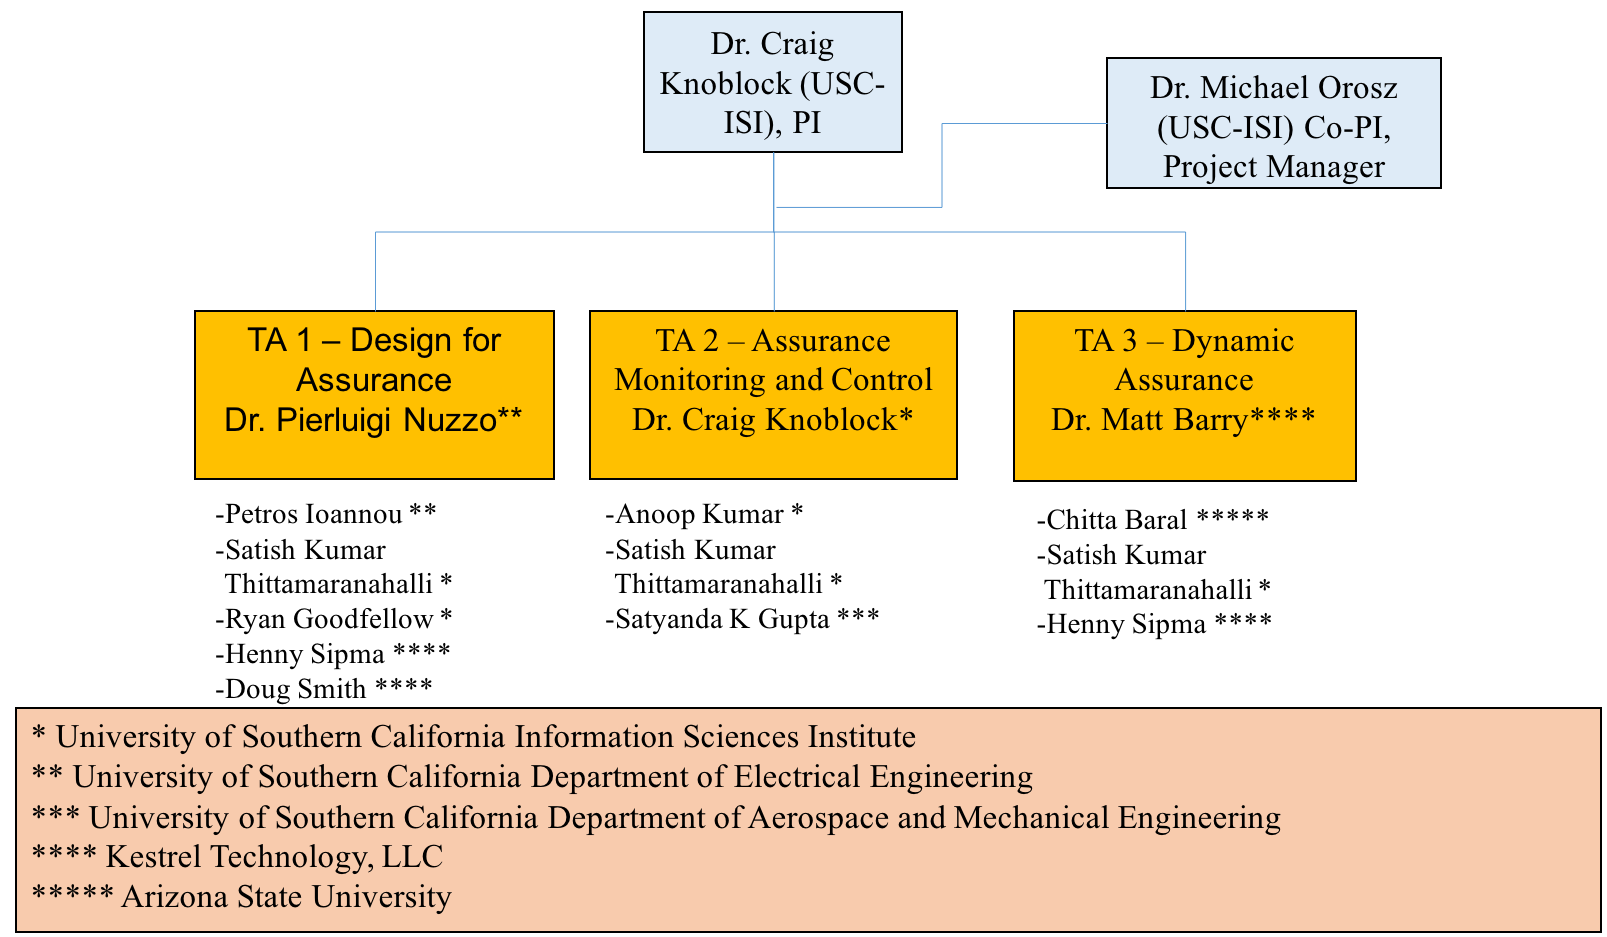
\includegraphics[width=6.0in]{./org-chart2.png}
\caption{\small Organization Chart}
\label{fig:org_chart}
\end{figure}

Coordination: To maximize collaboration and reduce risk to project failure from lack of communication and technical exchange, we plan to employ a wide variety of working styles and communication/coordination so that all can contribute.  At the core of our project will be regularly scheduled meetings bridging the diversely distributed team (Table~\ref{fig:Collaboration_Table}).  These meetings will address project status, identify challenges, implement risk mitigation strategies and participate in technology exchanges and system integration efforts (when appropriate)

\begin{table}[ht]
\caption{\small Project Meetings and Events}
  \centering
  {\footnotesize
\begin{tabular}{|m{3.15in}|m{3in}|} 
\hline
\textbf{Meeting} & \textbf{Frequency} 
\\\hline
Conference calls among investigators (discuss project status, address concerns and project risks) & Weekly
\\
\hline
Technical exchange and coordination meetings using Bluejeans or another videoconference technology & At least twice a month and more frequently as needed
  \\ 
\hline
Face-to-Face meetings (prior to P/I and demonstration meetings) & Every 3 to 6 months and more frequently (especially at the beginning of the project) as needed
 \\\cline{1-2}

\hline
\end{tabular}
}
\label{fig:Collaboration_Table}
\end{table}

\begin{table}[tbhp]
\caption{\small Key Project Team Member Responsibilities}
  \centering
  {\footnotesize
\begin{tabular}{| m{.75in} | m{3.9in}| m{1.5in}|} 
\hline
\textbf{Key Member} & \textbf{Responsibilities} & \textbf{Tasks} 
\\\hline
Dr.\ Craig Knoblock  & Principal Investigator responsible for project, leads TA 2 – Assurance Monitoring and Control.  Will lead the overall project and lead the TA2 team.  Served as the PI on many DARPA projects and has sucessfully led many large teams.    Effort on project:  25\% &
1.1.6, 1.2.2 1.2.3, 1.2.4, 1.3.4, 1.4.1, 
2.1.6, 2.2.2 2.2.3, 2.2.4, 2.3.4, 2.4.1, 
3.1.6, 3.2.2, 3.2.3, 3.2.4, 3.3.4, 3.4.1
\\
\hline
Dr.\ Michael Orosz & Co-Principal Investigator responsible managing the day-to-day operations of the project, assist technical teams as needed, coordinate with TA4 teams.    Has led many large complex multi-disciplined/multi-organizational projects in academic and industry environments.  Effort on project: 50\%
& 1.1.6, 2.1.6, 3.1.6, 1.4.1, 2.4.1, 3.4.1
  \\ 
\hline
Dr.\ Pierluigi Nuzzo 
& 
Co-Principal Investigator.  Leads the TA 1 - Design for Assurance team and conducts research on the formal methods for the design of the TA1 system.  Research experience on methodologies and tools for the design of cyber-physical systems; contracts, interfaces, and compositional methods for embedded system design; the application of automated formal methods and optimization theory to problems in embedded and cyber-physical systems.  Effort on project: 2 months/year (16.6\%)
& 
1.1.1, 2.1.1, 3.1.1 \\
\hline
Dr.\ Matthew Barry
& 
Key personnel.  Leads the TA 3 – Dynamic Assurance.   He will conduct the research on the dynamic assurance case language editors and parsers, the run-time system, and system integrations. Effort on project:  66\%
& 
1.3.2, 2.3.2, 3.3.2\\
\hline
Dr.\ Chitta Baral
& 
Key personnel responsible for learning assurance rules, supporting assurance rules with uncertainty and improving solver speed.  Expertise on ASP solvers, which will be used to reason about the assurance cases. Effort on project: 20\%
& 
1.3.1, 2.3.1, 3.3.1 \\
\hline
Dr.\ Doug Smith 
& 
Key personnel will support formal methods aspects of TA1, and lead the effort on abstract refinement. Expertise in field of automated correct-by-construction program generation.    Effort on project: 40\%
& 
1.1.5, 2.1.5, 3.1.5 \\
\hline
Dr.\ Henny Sipma
& 
Key personnel who will support the program verification tasks under TA1.  Will lead the effort on program verification.   Effort on project:  45\%
& 
1.1.5, 2.1.5, 3.1.5, 1.3.2, 2.3.2, 3.3.2 \\
\hline
Dr.\ Petros Ioannou
& 
Key personnel responsible providing and extending the assurance test bed, which will be available at the start of the project for autonomous vehicles.   Effort on project: 1 month/year (8.3\%)
& 
1.1.2, 2.1.2 (optional), 3.1.2 (optional)
\\
\hline
Dr.\ Satyandra Kumar Gupta
& 
Key Personnel providing autonomous command and control expertise to the TA-2 team.   Will lead the research on safety aware learning on TA2.   Past research on physics-aware decision making to facilitate automation.  Effort on project: 1 month/year (8.3\%)
& 
1.2.1, 2.2.1, 3.2.1 \\
\hline
Dr.\ Anoop Kumar 
& 
Key personnel providing support to the TA 2 project team.  Will lead the research on monitoring \& control and detecting distribution shifts.  Effort on project: 50\%
& 
1.2.1, 1.2.2, 1.2.3, 1.2.4, 2.2.1, 2.2.2, 2.2.3, 2.2.4, 3.2.1, 3.2.2, 3.2.3, 3.2.4\\
\hline
Dr.\ Satish Thittamaranahalli
& 
Key personnel developing scalable algorithms for TA1, TA2, and TA3 project teams.  Has extensive experience on scalable algorithm design, machine learning, and constraint reasoning.  Effort on project: 50\%
& 
1.2.1, 1.2.2, 1.2.3, 1.2.4, 2.2.1, 2.2.2, 2.2.3, 2.2.4, 3.2.1, 3.2.2, 3.2.3, 3.2.4, 1.1.4, 2.1.4, 3.1.4 \\
\hline
Dr.\ Ryan Goodfellow
& 
Key personnel providing support to the TA-1 project. Will lead the research on simulation-based testing.  Has extensive experience on simulation-based testing.  Effort on project:  30\%
& 
1.1.3, 2.1.3, 3.1.3 \\

\cline{1-2}

\hline
\end{tabular}
}
\label{fig:Table_Mgmt}
\end{table}



\newpage
\section{Personnel, Qualifications and Commitment}

{\bf Dr.\ Craig Knoblock}, the PI on this effort, is a Research Professor of both Computer Science and Spatial Sciences at the University of Southern California (USC) and Director of the Intelligent Systems Division at the USC Information Sciences Institute.   He received his Ph.D. from Carnegie Mellon University in computer science. 
%His research focuses on techniques for describing, acquiring, and exploiting the semantics of data.  
In previous projects he has worked on developing  scalable approaches to execution monitoring, accurate detection of sensor failures, and   automatic modeling and reconstruction of sensors.  He has published more than 300 journal articles, book chapters, and conference papers on these topics.  Dr. Knoblock is a Fellow of the Association for the Advancement of Artificial Intelligence (AAAI), a Distinguished Scientist of the Association of Computing Machinery (ACM), a Senior Member of IEEE, past President and Trustee of the International Joint Conference on Artificial Intelligence.
%and winner of the 2014 Robert S. Engelmore Award.  

{\bf Dr.\ Michael Orosz}, a Co-PI on this effort, is a Research Associate Professor of Civil and Environmental Engineering at the University of Southern California (USC) and Research Director of the Decision Systems Group at the USC Information Sciences Institute.  Dr. Orosz has over 30 years’ experience in commercial and government software development, basic and applied research, project management, academic research and has developed and deployed several commercially successful products.  His research interests are in machine learning and decision analytics as applied to intelligence analysis and autonomous command and control such as smart building controls.    Dr. Orosz has extensive experience in managing large complex multi-disciplined/multi-teamed research projects. %funded by DARPA, DHS, DoD, DoE, Industry, NASA, NRO, NSA and ONR.   
He received his Ph.D. in computer science from the University of California, Los Angeles.

{\bf Dr.\ Pierluigi Nuzzo}, a Co-PI on this project, is an Assistant Professor in the Department of Electrical Engineering at the University of Southern California. He received the Ph.D. in Electrical Engineering and Computer Sciences from the University of California at Berkeley. 
%in 2015, and the Laurea degree (MS) in electrical engineering (summa cum laude) from the University of Pisa, Italy, and the Sant'Anna School of Advanced Studies, Pisa, Italy.
%
%He has four years of research experience in analog and mixed signal circuit design as a researcher at IMEC, Leuven, Belgium, and over 10 years experience in design methodologies and tools for mixed-signal integrated circuits and cyber-physical systems, as a researcher at the University of Pisa, IMEC, UC Berkeley, and USC. 
His research interests
include: methodologies and tools for cyber-physical system and mixed-signal
system design; contracts, interfaces and compositional methods for embedded
system design; the application of formal methods and optimization theory to problems in embedded and cyber-physical systems and electronic design automation. 
%
Prof. Nuzzo received %First Place in the operational category and Best Overall
%Submission in the 2006 DAC/ISSCC Design Competition, 
a Marie Curie Fellowship
from the European Union in 2006, 
the University of California at Berkeley EECS
departmental fellowship in 2008, 
%the University of California at Berkeley Outstanding Graduate Student Instructor Award in 2013, 
the IBM Ph.D.
Fellowship in 2012 and 2014, 
%the Best Paper Award from the International Conference on Cyber-Physical Systems (ICCPS) in 2016, 
and the David J.~Sakrison Memorial Prize in 2016 for his doctoral research. 
%He is an author of 1 patent and over 60 publications.

{\bf Dr.\ Satyandra K. Gupta} is Smith International Professor in the Department of Aerospace and Mechanical Engineering at the University of Southern California. %Prior to joining the University of Southern California, he was a Professor in the Department of Mechanical Engineering and the Institute for Systems Research at the University of Maryland. He was the founding director of the Maryland Robotics Center and the Advanced Manufacturing Laboratory at the University of Maryland. 
He served as a program director for the National Robotics Initiative at the National Science Foundation from September 2012 to September 2014.  Dr. Gupta's interest is in the area of physics-aware decision making to facilitate automation. He has published more than 300 technical articles. He is a fellow of the American Society of Mechanical Engineers (ASME) and editor of ASME Journal of Computing and Information Science in Engineering. Dr. Gupta has received the Young Investigator Award from the Office of Naval Research in 2000, CAREER Award from the National Science Foundation in 2001, Presidential Early Career Award for Scientists and Engineers (PECASE) in 2001, Invention of the Year Award at the University of Maryland in 2007, Kos Ishii-Toshiba Award from ASME in 2011, and Excellence in Research Award from ASME in 2013.%, and Distinguished Alumnus Award from Indian Institute of Technology, Roorkee in 2014. %He has also received seven best paper awards at conferences.

{\bf Ryan Goodfellow} is a computer scientist at ISI working in combined cyber physical simulation and emulation platform development. His formal background is in simulation algorithms and modeling techniques using differential-algebraic equations (DAE). He has applied this knowledge in the CPS space by integrating DAE modeling languages and simulation engines with network testbeds to create comprehensive scientific experimentation platforms for cyber-physical systems. These experimentation platforms have been used in the power grid research space. %Ryan is a lead developer on the Deter network testbed, with a strong background in networked and distributed systems engineering. %He is also a combat veteran, serving as a non-commissioned officer and SIGINT team lead for a multi-functional intelligence team in Afghanistan.

{\bf Dr.\ Petros Ioannou} is a Professor in the Department of Electrical Engineering, Director of the Center for Advanced Transportation Technologies and Associate Director for Research for the DOT supported University Transportation Center at USC. He received his MS and PhD from the University of Illinois at Urbana Champaign in Mechanical and Electrical Engineering, respectively. His research interests are in robust adaptive control, vehicle dynamics and control, human factors and safety, automated vehicles, nonlinear systems and Intelligent transportation Systems.  He received the 2016 IEEE Transportation Technologies field award and the 2016 IEEE Control system society Transition to Practice Award. He is a Fellow of IEEE, IFAC and IET and author/coauthor of 8 books and over 400 papers.

{\bf Dr.\ Matthew Barry} will serve as lead for the TA3 tasks. %He will implement the dynamic assurance case language editors and parsers, the run-time system, and system integrations.  He will implement the assurance case arguments and the API for updating argument structure and content.  
Dr. Barry currently is CEO at Kestrel Technology LLC, and previously spent 20 years in NASA space mission operations at the Jet Propulsion Lab and Johnson Space Center.  At NASA Headquarters he led the introduction of dependability case requirements and plans for flight computing systems in upcoming manned space exploration missions, as well as the development of Agency-level software-related safety-critical control system requirements.  He recently served as a Principal Investigator on DHS/Cyber S\&T STAMP (Static Tool Analysis Modernization Program), DARPA CSFV (Crowd Sourced Formal Verification), three NASA Aeronautics R\&D projects, and the AFRL-sponsored Static Analysis of Numerical Algorithms project.  Dr. Barry earned BSME, MS, and PhD degrees in mechanical engineering, and an MBA degree, from Rice University.  

{\bf Dr.\ Henny Sipma} will support the program verification tasks under TA1.  %She is the key person behind the company's {\em KT Advance\/} and {\em KT Transferal\/} static analysis products, and the designer and programmer of the company's core {\em CodeHawk\/} abstract interpretation engine. 
Dr. Sipma currently is the CTO at Kestrel Technology LLC.  She has spent the past 10 years with Kestrel Technology as a static analysis expert; previously developed and taught static analysis techniques as senior research associate at Stanford University for eight years; and developed industrial process controls as an senior systems analyst at Shell.  She has been Principal Investigator or company lead on several recent R\&D projects for Federal agencies, including two projects under the IARPA STONESOUP (Securely Taking On New Executable Software of Uncertain Provenance) program; the DHS Cyber S\&T Gold Standard project; and the DARPA-sponsored STAC (Space-Time Analysis for Cybersecurity) and MUSE (Mining and Understanding Software Enclaves) programs.  Dr. Sipma earned 
%a BS degree in chemistry and an MS degree in chemical engineering at the University of Groningen in The Netherlands, and 
MS and PhD degrees in computer science from Stanford University.  

{\bf Dr.\ Douglas R.\ Smith} will support formal methods aspects of TA1, including the enforcement of safety properties and the generation of monitors.  He is President of Kestrel Technology LLC and Principal Scientist at Kestrel Institute.  He is a Fellow of the American Association of Artificial Intelligence (AAAI) and an ASE Fellow (Automated Software Engineering).  From 1986 to 2000, he taught an advanced graduate course on correct-by-construction software development at Stanford.  
%Dr. Smith has led the development of a series of software synthesis systems, including KIDS (Kestrel Interactive Development System), Specware, Designware, and Planware. 
%Applications domains have included a variety of complex high-performance planners and schedulers for the US Air Force.  He leads current projects on the generation of air mission plans and cyberoperations.  
Other recent projects focused on automated policy enforcement \cite{SmithD0703,SmithD08}, synthesis of secure network protocol codes, and the synthesis of high-performance constraint-solvers\cite{SmithD08c,SmithD13}.  Dr. Smith has over 30 years experience in the field of automated correct-by-construction program generation and has published over 100 papers. He has one patent.  He received the Ph.D. in Computer Science from Duke University% in 1979.  

{\bf Dr. Chitta Baral} is a Professor in the Department of Computer Science and Engineering at Arizona State University. He will support the TA3 efforts on Learning assurance rules, supporting assurance rules with uncertainty and improving solver speed. Dr. Baral has expertise in various aspects of autonomy and Artificial Intelligence. 
He wrote the first book on answer set programming (published by Cambridge University Press) the formal language behind our assurance rules. Some of his other works relevant to this proposal are: goal specification for autonomous systems, automatic construction of control rules for autonomous systems that satisfy given goals, combining machine learning with reasoning in various contexts, including image understanding. %He is the President of KR Inc. He is an associate editor of AIJ and has been an associate editor of JAIR.

{\bf Dr.\ Satish Kumar Thittamaranahalli (T. K. Satish Kumar)} leads the Collaboratory for Algorithmic Techniques and Artificial Intelligence (CATAI) at USC's Information Sciences Institute. He has published over 60 papers on numerous topics in Artificial Intelligence spanning such diverse areas as Constraint Reasoning, Planning and Scheduling, Probabilistic Reasoning, Robotics, Combinatorial Optimization, Approximation and Randomization, Heuristic Search, Model-Based Reasoning, Knowledge Representation and Spatio-Temporal Reasoning. %He %has served on the Program Committees of many international conferences in Artificial Intelligence
He and is a winner of the 2016 Best Robotics Paper Award and the 2005 Best Student Paper Award from the International Conference on Automated Planning and Scheduling. 
Dr. Kumar received his PhD in Computer Science from Stanford University. %In the past, he has also been a Visiting Student at the NASA Ames Research Center, a Postdoctoral Research Scholar at the University of California, Berkeley, a Research Scientist at the Institute for Human and Machine Cognition, a Visiting Assistant Professor at the University of West Florida, and a Senior Research and Development Scientist at Mission Critical Technologies.

\textbf{Dr.\ Anoop Kumar} is a senior computer scientist at USC ISI and has broad expertise in machine learning, statistical modeling, and software engineering.  Dr.\ Kumar is the technical lead on the DARPA RSPACE program and has played a vital role in developing a system that fuses air operations data from multiple sources, maintains world state, and issues warnings. Previously, he led the research and development of the BBN’s election forecasting system for the IARPA OSI program. %Dr.\ Kumar played a significant role in the DARPA DEFT program by developing a model to support integration of output from multiple NLP algorithms. He has contributed at the development to management levels on government research contracts and commercial projects. 
Dr.\ Kumar helped design and develop BBN's commercially available, hosted speech and medical transcription services offering. 

\begin{table}[!tbh]
\begin{footnotesize}
\vspace{-0.1in}

\begin{tabular}{lll}
\begin{tabular}[t]{|l|@{}c@{}|@{}c@{}|@{}c@{}|@{}c@{}|} \hline
Project & Status & \multicolumn{3}{ c| }{Hours} \\ \cline{3-5}
& & P1 & P2 & P3 \\ \hline



\multicolumn{5}{ |c| }{ \textbf{Craig Knoblock} } \\ \cline{1-5}
Safeguard & Pro & 770 & 641 & 641 \\ \cline{1-5}
ELICIT & Cur & 308 & 256 & 120 \\ \cline{1-5}
WTNIC & Cur & 11 & 0 & 0 \\ \cline{1-5}
EFFECT & Cur & 641 & 107 & 0 \\ \cline{1-5}
LinkedMaps & Cur & 203 & 25 & 0 \\ \cline{1-5}
PRINCESS & Cur & 608 & 96 & 0 \\ \cline{1-5}
SCHARP & Cur & 481 & 54 & 0 \\ \cline{1-5}
MINT & Pen & 650 & 534 & 285 \\ \cline{1-5}

\multicolumn{5}{ |c| }{ \textbf{Michael Orosz} } \\ \cline{1-5}
Safeguard & Pro & 1560 & 1300 & 1300  \\ \cline{1-5}
SMC/SY & Cur & 1803 & 0 & 0  \\ \cline{1-5}

\multicolumn{5}{ |c| }{ \textbf{Matthew Barry} } \\ \cline{1-5}
Safeguard & Pro & 2078 & 1690 & 1554 \\ \cline{1-5}
Starlite & Cur & 1840 & 1692 & 0 \\ \cline{1-5}



\multicolumn{5}{ |c| }{ \textbf{Anoop Kumar} } \\ \cline{1-5}
Safeguard & Pro & 1560 & 1300 & 1300 \\ \cline{1-5}

\end{tabular}
&
\begin{tabular}[t]{|l|@{}c@{}|@{}c@{}|@{}c@{}|@{}c@{}|} \hline
Project & Status & \multicolumn{3}{ c| }{Hours} \\ \cline{3-5}
& & P1 & P2 & P3 \\ \hline

\multicolumn{5}{ |c| }{ \textbf{Pierluigi Nuzzo} } \\ \cline{1-5}
Safeguard & Pro & 520 & 433 & 433  \\ \cline{1-5}
Mirage & Cur & 433 & 0 & 0  \\ \cline{1-5}

\multicolumn{5}{ |c| }{ \textbf{Satyandra Gupta} } \\ \cline{1-5}
Safeguard & Pro & 260 & 217 & 217 \\ \cline{1-5}
Human   & Cur & 22 & 0 & 0 \\ \cline{1-5}
Vehicles & Cur & 36 & 0 & 0 \\ \cline{1-5}
Robot & Cur & 116 & 0 & 0 \\ \cline{1-5}
Assembly & Cur & 33 & 0 & 0 \\ \cline{1-5}
Solar & Cur & 4 & 0 & 0 \\ \cline{1-5}

\multicolumn{5}{ |c| }{ \textbf{Petros Ioannou} } \\ \cline{1-5}
Safeguard & Pro & 260 & 217 & 217 \\ \cline{1-5}
CPS & Cur & 130 & 0 & 0 \\ \cline{1-5}

\multicolumn{5}{ |c| }{ \textbf{Ryan Goodfellow} } \\ \cline{1-5}
Safeguard & Pro & 936 & 780 & 780 \\ \cline{1-5}
STEAM & Cur & 416 & 0 & 0 \\ \cline{1-5}


\end{tabular}
&
\begin{tabular}[t]{|l|@{}c@{}|@{}c@{}|@{}c@{}|@{}c@{}|} \hline
Project & Status & \multicolumn{3}{ c| }{Hours} \\ \cline{3-5}
& & P1 & P2 & P3 \\ \hline

\multicolumn{5}{ |c| }{ \textbf{Chitta Baral} } \\ \cline{1-5}
Safeguard & Pro & 659 & 485 & 485 \\ \cline{1-5}
PostdocBP & Cur & 176 & 0 & 0 \\ \cline{1-5}
Languages & Pen & 528 & 264 & 264 \\ \cline{1-5}
CAREER & Pen & 88 & 44 & 44 \\ \cline{1-5}
CHS & Pen & 510 & 255 & 0 \\ \cline{1-5}

\multicolumn{5}{ |c| }{ \textbf{Doug Smith} } \\ \cline{1-5}
Safeguard & Pro & 1222 & 984 & 840 \\ \cline{1-5}
RSPACE & Cur & 342 & 0 & 0 \\ 
\cline{1-5}
PLANX & Cur & 154 & 0 & 0 \\ 
\cline{1-5}
HACCS & Pen & 923 & 769 & 769 \\ 
\cline{1-5}

\multicolumn{5}{ |c| }{ \textbf{Henny Sipma} } \\ \cline{1-5}
Safeguard & Pro & 1372 & 962 & 840 \\ \cline{1-5}
STAC & Cur & 797 & 0 & 0 \\ \cline{1-5}

\multicolumn{5}{ |c| }{ \textbf{Satish Thittamaranahalli} } \\ \cline{1-5}
Safeguard & Pro & 1560 & 1300 & 1300 \\ \cline{1-5}
MapF & Cur & 103 & 103 & 0 \\ \cline{1-5}

\end{tabular}
\end{tabular}

\end{footnotesize}
\caption{Individual commitments of key personnel}
\label{tab:Commitments}
\vspace{-0.2in}
\end{table}

\clearpage
\newpage
\section{Capabilities}


%\subsection{University of Southern California}
USC has strengths in number of areas that are closely related to the proposed work:
\begin{itemize}[itemsep=0pt,leftmargin=*]
\item Dr.\ Nuzzo 
%has over 10-year research experience in embedded system design, from mixed-signal chip design (analog-to-digital converters, frequency synthesizers, software-defined radio), to methodologies and tools for mixed-signal integrated circuits and Cyber-Physical Systems (CPSs), and the application of formal methods and optimization theory to problems in embedded and cyber-physical systems and electronic design automation.  
%His doctoral work 
has done extensive research on contracts and compositional methods for heterogeneous system design and design space exploration, with application to aircraft electric power systems and environmental control systems. His work has helped transition rigorous system design foundations, innovative design methodologies, and new systems engineering paradigms to industry (IBM, United Technologies). 
\item Dr.\ Satyandra K. Gupta has worked on autonomous surface vehicles, autonomous ground vehicles for operation on rugged terrains, and autonomous flapping wing aerial vehicles.   His group has developed a hierarchal decision making approach for realizing autonomous systems. 
%This approach combines task planning and assignment, deliberative trajectory planning, reactive collision avoidance behaviors, and trajectory tracking control layers. 
His group has also developed new methods for learning reactive behaviors in adversarial environments and COLREGS compliant trajectory planning. \item Dr.\ Knoblock has developed methods that learn the relationships between sensors to both identify failures and changes in sensor and reconstruct those sensors, providing estimates of the accuracy of the reconstructed sensors.  
\item Ryan Goodfellow has extensive experience in simulation based testing through high-fidelity CPS testbed environment development and operation, using the Deter network testbed as the core which has supported several large scale government projects from a variety of agencies and thousands of users. %we have developed sophisticated CPS experiments under programs such as NFS RIPS, NIST SmartCities and the DHS Cybersecurity showcase.
\item Dr.\ Ioannou %helped  design and implement adaptive cruise control systems in collaboration with Ford Motor Company, which was commercialized four years before any other company. He 
worked on several DOT funded projects on automated vehicles and intelligent highway systems where he demonstrated his vehicle control designs for safety and performance on actual automated vehicles in test trucks and I-15 highway.
\item Drs.\ Knoblock, Kumar, and Thittamaranahalli have developed highly scalable approaches for monitoring message traffic to identify potential problems and issue warnings and alerts. 
\item Dr. Thittamaranahalli has developed state-of-the-art methods for efficiently solving large-scale search and optimization problems. %These techniques will be applicable in TA2 for safety-aware learning and planning, in TA2 for assurance monitoring and control, and in TA3 for dynamic assessment of assurance cases.

\end{itemize}
%\subsection{Kestrel Technology LLC}

Kestrel Technology's strength is in program analysis, specifically static analysis of both source and binary targets.  The company performs applied R\&D and product development for a variety of static analysis applications  pivoting primarily on the abstract interpretation technique.  The company recently initiated development of program analysis applications using logical equivalence techniques. As a provider of verification evidence in the form of mathematical proofs, the company also has expertise in the design and development of assurance case arguments for high-integrity systems using such evidence. %The company is engaged in a partnership with Wind River Systems to develop program analysis tools for its embedded system developers.  Many of Wind River's customers must develop their products under safety and certification standards, including those using safety cases.  

   

%\subsection{Arizona State University}
Chitta Baral at Arizona State University has developed various software to learn assurance rules and various ASP solvers, which he has made available as open-source.

Most of the software carried forward for implementation or derivation is open source.  The single exception is Kestrel Technology's {\it KT Advance\/} static analysis tool (TA1), in particular the abstract interpretation engine therein, which is company proprietary and is US EAR export-controlled.   
%Owing to mixed funding for the development of that technology 
We will continue to provide the Federal government a restricted use license for that particular item.

There are no specialized facilities, data, or GFE required for this effort. 

\include{sow}
\include{milestones}

% \section{Level of Effort by Task \textcolor{red}{[Mike/Lisa - 1 pages]}}

% \textcolor{blue}{
% \begin{itemize}
% \item Will be a separate spreadsheet
% \item
% \end{itemize}
% }

\include{appendix_a}

%\section{Appendix B \textcolor{red}{[No Page Count]}}

\section{References}
\bibliographystyle{acm} 
\bibliography{TA3/ta3,TA2/ta2,TA1/ta1}
\end{document}
%%\documentclass[a4paper]{article}
%\documentclass[12pt]{article}
\documentclass[12pt]{dod-blank}

%% Language and font encodings
\usepackage[english]{babel}
\usepackage[utf8x]{inputenc}
\usepackage[T1]{fontenc}

%% Sets page size and margins
%%\usepackage[a4paper,top=3cm,bottom=2cm,left=3cm,right=3cm,marginparwidth=1.75cm]{geometry}
%\usepackage[top=1in, bottom=1in, left=1in, right=1in]{geometry}



%% Useful packages
\usepackage{amsmath}
\usepackage{graphicx}
  \graphicspath{{.}{./image/}}
  \DeclareGraphicsExtensions{.png,.jpg} 
\usepackage[colorinlistoftodos]{todonotes}
\usepackage[colorlinks=true, allcolors=blue]{hyperref}
\usepackage{tabularx}
\usepackage{multirow}
\usepackage{tabulary}
\usepackage{float}
\usepackage{wrapfig}
\usepackage[export]{adjustbox}
\usepackage{comment}
\usepackage{tabularx}
\usepackage{multirow}
\usepackage{tabulary}
\usepackage{enumitem}

\usepackage{listings}
\usepackage{color}
\usepackage{array}
\usepackage{subcaption}
\usepackage{xcolor}




\renewcommand{\textfraction}{0}
\renewcommand{\topfraction}{1.0}
\renewcommand{\bottomfraction}{1.0}

\usepackage{longtable}
%% macros
\newif\iffinal
\finaltrue
\iffinal
  
    \newcommand\baareq[1]{}
    \newcommand\baades[1]{}
 
 
\else
    \definecolor{darkgreen}{rgb}{0,0.4,0}
    \definecolor{darkcyan}{rgb}{0,0.4,0.4}
    \definecolor{darkblue}{rgb}{0,0,0.5}
    
    \newcommand\baareq[1]{{\color{darkcyan}[\textbf{Requirement:} #1]}}
    \newcommand\baades[1]{{\color{darkcyan}[\textbf{Description:} #1]}}
 
\fi




\def\naive{na\"{\i}ve}



\lstset{ 
  backgroundcolor=\color{white},   % choose the background color; you must add \usepackage{color} or \usepackage{xcolor}
  basicstyle=\footnotesize\ttfamily,            % the size of the fonts that are used for the code
  breakatwhitespace=false,         % sets if automatic breaks should only happen at whitespace
  breaklines=true,                 % sets automatic line breaking
  captionpos=b,                    % sets the caption-position to bottom
  commentstyle=\color{mygreen},    % comment style
  % deletekeywords={...},            % if you want to delete keywords from the given language
  escapeinside={\%*}{*)},          % if you want to add LaTeX within your code
  extendedchars=true,              % lets you use non-ASCII characters; for 8-bits encodings only, does not work with UTF-8
  frame=single,	                   % adds a frame around the code
  keepspaces=false,                 % keeps spaces in text, useful for keeping indentation of code (possibly needs columns=flexible)
  keywordstyle=\color{blue}\bfseries\underbar,       % keyword style
  language=Prolog,                 % the language of the code
  % morekeywords={if,and},        % if you want to add more keywords to the set
  numbers=none,                    % where to put the line-numbers; possible values are (none, left, right)
  numbersep=5pt,                   % how far the line-numbers are from the code
  numberstyle=\tiny\color{mygray}, % the style that is used for the line-numbers
  rulecolor=\color{black},         % if not set, the frame-color may be changed on line-breaks within not-black text
  showspaces=false,                % show spaces everywhere adding particular underscores; it overrides 'showstringspaces'
  showstringspaces=false,          % underline spaces within strings only
  showtabs=false,                  % show tabs within strings adding particular underscores
  stepnumber=2,                    % the step between two line-numbers. If it's 1, each line will be numbered
  stringstyle=\color{mymauve},     % string literal style
  tabsize=2,	                   % sets default tabsize to 2 spaces
  title=\lstname                   % show the filename of files included with \lstinputlisting; also try caption instead of title
}

% apply trick for additional keywords for our AC DSL
\lstset{
	emph={for, if, and, or},
    emphstyle={\color{blue}\bfseries\underbar}
}




\title{DARPA Assured Autonomy}
\author{Technical Volume- \textcolor{red}{Thirty-Eight (38) pages max}}

\begin{document}
\pagenumbering{roman}
\include{cover}

\newpage
\section{Table of Contents}
\tableofcontents

\newpage
\pagenumbering{arabic}
\section{Executive Summary}
As we rapidly move into a world where machine learning plays a central role in realizing autonomous systems, it is becoming increasingly important to develop techniques that assure that these systems will operate safely and perform as expected. Current approaches are limited to providing assurance for systems with limited or no  learning capabilities. In this context, DARPA's Assured Autonomy BAA seeks to \emph{develop rigorous design and analysis technologies for continual assurance of learning-enabled autonomous systems}. USC in collaboration with Kestrel Technology and ASU is pleased to submit a comprehensive TA1, TA2, and TA3 proposal entitled \emph{``Assured Autonomy for Learning Enabled Vehicles (Safeguard).''} We plan to provide an end-to-end solution to support autonomous systems with learning-enabled components, ranging from design technologies for assurance, to assurance monitoring and control techniques, to representation and online evaluation of assurance cases. We have assembled a strong team of experts that cover the range of technologies that are required to create such an end-to-end system. If successful, the project will provide the technologies for building the next-generation of learning-enabled autonomous systems.  The entire project will take four years and cost \textcolor{red}{\$??}, with an initial version completed at the end of Phase I and successive versions with additional capabilities and improved scalability at the end of Phase II and Phase III.  

In the remainder of this section, we first introduce an  unmanned surface vehicle scenario that will be used throughout the proposal to describe the approach.  Next, we describe our approach to design, monitoring, and dynamic assurance. Finally, we introduce the team involved in the project. 

\textbf{Motivating Scenario.} Consider an autonomous unmanned surface vehicle (USV) guarding a valuable asset in the ocean when an unknown vehicle  approaches the security perimeter, under challenging weather conditions. In this scenario, the USV is required to approach the intruding vehicle, issue a warning signal, and escort it to a safe distance from the controlled area. However, as the USV has no a priori knowledge of its external environment behaviors (e.g., water depth, waves, wind, current, visibility), pre-computing a feasible trajectory, let alone optimal, becomes a non-trivial problem. For trajectory planning, the USV must continuously perform the following tasks:
\begin{itemize}[itemsep=0pt,leftmargin=*]
 \item Sense the current state of the surrounding environment (e.g., water depth, waves, wind, current, visibility) and estimate its own maneuverability constraints (e.g., braking distance, available acceleration, maximum velocity, turning radius, turning rate, safety distance) based on the state of the environment;      
\item Sense the static obstacles in the sensor range and generate a traversability map;
\item Sense the moving obstacles and classify them;   
\item Predict future trajectories of moving obstacles; 
\item Determine if any of the COLREGS \cite{commandant1999international} rules will be in effect with respect to one or more of the nearby vessels and identify the vessels with the right of way.    
\end{itemize}
The above information will be used by the trajectory planner to compute an initial trajectory, which will be continuously refined as the USV gathers additional information.
% It is not possible for the USV to be tested in every possible environment. 
The USV will use learning enabled components to take  decisions as it encounters new situations, such as  
\begin{itemize}[itemsep=0pt,leftmargin=*]
\item Classifiers to identify moving obstacles based on physical appearance and motion signatures,
\item Algorithms to estimate the sensor capabilities in adverse weather conditions,   
\item Algorithms to accurately estimate uncertainty in the environment, 
\item Classifiers to generate traversability maps,
\item Prediction of external vessel behaviors based on motion histories, 
\item Reinforcement learning  to ensure COLREGS compliance of maneuvers,  
\item Algorithms to learning pursuit behaviors.  
\end{itemize}
Learning enabled components will interact with each other in complex ways, where a misclassification error in one component may eventually compromise the entire mission.   
% We will need to make sure that each learning enabled components has a run-time monitor that will ensure that the assumptions made by the learning-enabled component remain valid and prevent erroneous learning. 
% For example, if the vehicle is exhibiting significant error in trajectory tracking, then simply downgrading the trajectory tracking error value may not be a good option.  The failure of prediction of trajectory tracking error might be due to the presence of a significant wake caused by a nearby vessel. The presence of the nearby vessel can be used to explain the degradation in trajectory tracking performance. As the vessel moves away, we can expect the trajectory tracking performance to return to the predicted level.  
While exhaustive validation of learning-enabled cyber-physical systems (LE-CPSs) is a prohibitive task~\cite{Kalra16},
their complexity, heterogeneity, and highly dynamic nature
make it challenging to even leverage existing model-based development techniques to effectively assess system correctness 
% dependability, 
at design time or enforce it at runtime.

\textbf{Design for Assurance.} Safeguard uses a platform-based design approach~\cite{Nuzzo15b} to organize the design process for a LE-CPS and to build assurance cases. Composite models are developed at several levels of abstraction,
from top-level system requirements and safety constraints down to the
implementation level.  Intermediate levels add detail to the levels
above.  The different levels are connected by refinement mappings that
allow properties established at one level to be preserved at the next
level (see Figures~\ref{fig:methodology} and~\ref{fig:assurance}).

Contracts are used to formally specify components and composite models
in terms of (1) Assumptions -- the assumed behaviors of the
environment and the behaviors of other components, and (2) Guarantees
-- the behavior properties that a model guarantees if it operates in a
context that satisfies its assumptions.  A calculus of contracts
allows horizontal composition of contracts to generate contracts for
composite models.  Vertical contracts are used to specify the mapping
or refinement relation between models at different levels of
abstraction.  The system design process starts with a high-level
contract that expresses overall system assumptions and requirements.
Subsequent levels express models with increasing detail until the
lowest level expresses the system in terms of hardware components and
their software controllers.

The assurance case for a CPS arises from the horizontal and vertical
structure of the design in several ways.  The components used within a
particular level are either (1) synthesized using
correct-by-construction design tools together with proofs, (2) derived
statically or dynamically using safety-aware machine-learning
techniques, (3) written manually and verified by analysis tools, or
(4) written manually and validated by extensive testing.  The
assurance case for the whole reflects its compositional structure.  We
anticipate that well-specified contracts together with the calculus of
contracts will eliminate well-known problems with unexpected emergent
behaviors in CPS systems.

The assurance case for the lowest-layer design arises from both the
intra-level assurance and from properties and their proofs that are
preserved under the refinement mapping from the top-level
requirements.  The refinement mappings between model layers will be
constructed using a variety of techniques.  A contract at an abstract
level can be mapped to a component or refined contract by (1)
retrieval of pre-verified components from a platform library, (2)
synthesis using correct-by-construction design and optimization tools,
or (3) manual coding to satisfy a contract.  The mapping of a
composite model will be composed from the mappings of its constituent
components or contracts.  When a composite model cannot be mapped
compositionally to the next level, it will be generated using
correct-by-construction design and optimization tools.

\textbf{Assurance Monitoring and Control.}
We provide an integrated framework for safety-aware learning, assurance monitoring and control, detecting distribution shifts. Three major components offer an efficient TA2 architecture as well as interfaces with TA1 and TA3, that is, (a) safety-aware learning and planning, (b) assurance monitors for guarding architectural and safety constraints; and (c) distribution shift detection.

We will develop a new learning-enabled online decision-making framework that allows opportunistically composing a sequence of actions (maneuvers) to reduce uncertainty in the system capability model without suspending the progress toward the mission goals or compromising safety. Each candidate action is evaluated based on three criteria: (1) the risk of violating a safety constraint using the current uncertainties in the parameter estimates; (2) its relevance to the mission goals; (3)  its expected information gain, i.e., reduction in uncertainty, with respect to the parameter estimates. These evaluations are combined to produce a cumulative mission utility value for each action that drives our learning-enabled decision-making framework. The problem of generating and evaluating sequences of actions can be posed in several way. For example, it can be solved using a branch-and-bound search method like Anytime A*, or formulated with the finite-horizon Markov Decision Process (MDP) framework. We will develop new scalable search strategies to solve this problem efficiently, by potentially evaluating a recent method developed at USC, called FastMap, that can significantly improve the execution time. 

We will develop monitors for architectural and safety constraints. 
% While these constraints can be checked over and over again as sensor information flow in, this naive strategy accounts for a lot of computational overhead. 
To achieve scalability and decrease the overhead, we propose the application of a technique that we currently use in DARPA's RSPACE program, which leverages a physical model of the vehicles dynamics and its interactions with the environment to efficiently determine the readout frequency. We propose two  extensions of this basic idea. First, we will use the theory of Variable Elimination to prioritize which variables to monitor, e.g., controllable, versus uncontrollable, adversarially controlled, or unobservable variables. Second, we invoke the dynamic assessment of assurance cases only when needed. This  decreases the number of times dynamic assessment of assurance cases is initiated as well as the communication bandwidth between the TA2 and TA3 components.

Finally, we will identify a distribution shift by combining statistical and machine learning techniques to differentiate between environmental and sensor changes. We will exploit a categorization of the shifts based on their cause and duration as well as extend our earlier work on detecting and mitigating sensor failures for all types of monitored variables.  

\textbf{Dynamic Assurance:} The Safeguard {\em design for assurance\/} activity takes a systems-theoretic stance toward safety.  Consequently, it presumes that safety is an emergent property of the system, and that hazards can present themselves through unintended interactions and performance violations in addition to causal events such as component failures.  Our design approach includes consideration of intent as well as hazard analysis and mitigation.  The artifacts from these activities populate contracts and assumptions for the dynamic assurance case.  
We thus build safety into the product by working at a systems-level viewpoint, using lexicon and design patterns familiar to both hardware and software engineers; safety is an emergent property of the system, not an afterthought.  
As system behavior evolves during runtime owing to learning, threats, degradation, or some other factor, the dynamic assurance case identifies whether the safety constraints continue to be satisfied.  If not, it provides notifications or issues recovery instructions directly from a lookup table.

Our implementation of the dynamic assurance case employs a declarative knowledge base inference engine and a domain-specific language tailored to our approach.  We have used them successfully for assurance case tool sets and arguments, and will extend them to reason about uncertainty and learning.  Our approach to achieve scalability is to specialize solvers toward modularity and to take advantage of domain knowledge.  Specifically, we will develop answer set programming techniques for context-dependent learning for reasoning about the learning-enabled components as well as learning assurance rules.  We will develop new formalisms for uncertainty to include causality, using weights for computing probabilities, and probabilistic non-monotonicity.  To achieve scaling objectives we will implement specializations using modularity, weighted CSPs, and message passing. 

% The system safety constraints revealed from that design become the key elements of our dynamic assurance case.  Our verification tools ensure the constraints are relevant, identifiable, and their implementation and effect observable.  

\textbf{Team.} We have assembled a team that is exceptionally well-qualified to build the proposed Safeguard system.  The team will be led by Dr.\ Craig Knoblock, the Principal Investigator for the effort, who currently leads the Intelligent Systems Division at the Information Sciences Institute.  He has led many large DARPA and IARPA projects over the years and has a strong track record in conducting leading edge research and then transitioning the technology to commercial use.  He will be supported by Dr.\ Michael Orosz as the Project Manager, who also has  experience in managing large research projects and on autonomous systems.  The TA1 team will be led by Dr.\ Pierluigi Nuzzo, who is an expert in embedded system design methodologies and the  application of formal methods to cyber-physical systems.  The TA1 team also includes Dr.\ Doug Smith, who has spent many years working on scalable correct-by-construction techniques and Dr.\ Henny Sipma, who has significant experience in applying program verification methods to real-world problems.  The TA1 team also includes Ryan Goodfellow, who has done a large amount of work on simulation-based testing.  The TA2 team will be led by Dr.\ Knoblock who has worked on topics related to both monitoring and detecting distribution changes.  He will be supported by Dr.\ Satyandra Gupta, who is an expert on autonomous surface vehicles as well as on safety-aware learning. He will also be supported by Drs.\ Anoop Kumar and Satish Thittamaranahalli, who have also previously worked on efficient methods for execution monitoring.  The TA3 team will be lead by Dr.\ Matthew Barry, who has experience in creating the technologies for assurance cases.  He will be supported by Dr.\ Chitta Baral, who is an expert on ASP solvers and by Dr.\ Thittamaranahalli who is an expert on SAT solvers, both of which will be applied to provide scalable assurance case reasoning.  Finally, Dr.\ Petros Ioannou, who is an expert on control systems for autonomous vehicles will provide an autonomous vehicle platform, which will form the focus of our work until the TA4 teams provide additional vehicle platforms for development.  

\newpage
\section{Innovative Claims and Deliverables}

In this project we will develop and build an end-to-end system for assured autonomy.  This section describes the key innovations by technical area and then the overall deliverables of the project.

\paragraph{Design for Assurance}

\begin{itemize}[itemsep=0pt,leftmargin=*]
\item We address the LE-CPS design challenges via a holistic approach that can contextually generate design artifacts and assurance cases. We develop a compositional, contract-based modeling framework, methods, and tools to support the design process from system-level requirement capture,  formalization, and analysis, to the generation, testing, and continual monitoring of software and hardware artifacts in feedback loop with a physical process.

\item We develop compositional abstractions and interfaces (vertical contracts) that can  bridge heterogeneous formalisms and heterogeneous decomposition architectures to make system analysis and synthesis tractable, consistently combine different verification and synthesis methods at design time, and provide seamless support for dynamic assurance at run time. %We aim to quantitatively capture the confidence in the satisfaction of requirements under uncertain or unknown conditions, and resilience properties of  systems at different abstraction levels, to enable trade-off evaluation between resilience, performance, and cost.

\item We develop a unifying framework and efficient algorithms to reason about the combination of discrete and continuous dynamics and constraints in the presence of uncertainties in LE-CPS using a satisfiability modulo convex approach~\cite{Shoukry2017} for contract-based system verification and scalable trajectory planning.  

\item We provide an environment for high-fidelity CPS testing, in which production-ready software, e.g.,  safety-critical learning and control, may be deployed and tested 
% by extending the Cypress testbed environment \cite{Goodfellow2015Cypress:Systems} 
with time dilation facilities, so that it synchronizes with a physical simulation that is not necessarily running in real time, while still having the perception of real time.

\item We 
% These facilities allow a cyber system to be  
propose an approach for unanticipated behavior space identification and test coverage maximization which leverages results from the theory of differential algebraic equation (DAE)~\cite{Berger2013ControllabilitySurvey,Ilchmann2005ATheory,BergerOnSystems,Lamour2013} 
to prune the behavior search space and identify smaller regions of interest for efficient simulation-based testing. 
% We then compute the intersection of these two behavior spaces and restrict our simulation based testing search space to this subspace.
\end{itemize}

\paragraph{Assurance Monitoring and Control}

\begin{itemize}[itemsep=0pt,leftmargin=*]
\item 
%We integrate safety-aware learning into the overall decision making problem. The goal is to maximize mission utility without violating the safety constraints. 
Our safety-aware learning framework enables the system to opportunistically select and execute actions to assist the learning-enabled component in reducing model uncertainty without compromising safety or deviating from the mission goals. The value of uncertainty reduction is explicitly incorporated in the optimization process for selecting the best action.  
\item For safety-aware learning, we propose the idea of preprocessing the search space of the problem domain before queries and observations come in. With such a linear-time preprocessing phase, the performance of search and optimization algorithms can be significantly boosted. For example, in regular A* search, the intensional or extensional search space can be preprocessed in near-linear time to yield an embedding of each state as a point in Euclidean space~\cite{cujakk}. Then, when the query comes in, A* search can make use of these Euclidean distances as heuristic distances between two states to yield order-of-magnitude speedups. 
%In Anytime A* for safety-aware learning and planning, this leads to a significantly better quality of actions chosen within a time limit, and in the MDP framework, the same ideas can be used to improve the convergence of Bellman updates for safety-aware Reinforcement Learning.
\item As massive amounts of sensor information flow in, it is imperative for us to efficiently process this information for monitoring architectural and safety constraints. Building on our past work on similar tasks, we propose novel technologies for efficiently monitoring constraints. These algorithms can yield an exponential reduction in the amount of sensor data that needs to be processed. Doing this also reduces the message complexities between the various modules. %We also propose to use the theory of Variable Elimination (VE) to monitor constraints with uncontrollable, adversarially controlled, and/or unobservable variables. VE yields a substrate constraint to monitor that characterizes a dominant strategy of the controllable variables over the uncontrollable, adversarially controlled, and/or unobservable variables.
\item We will develop techniques to identify  distributional shifts and determine the underlying cause (e.g., change in environment, sensor failure,   etc.), as well as strategies for handling the various distributional shifts.   Notably, we propose to build on our past work and use compact representations to exploit historical data to identify distributional shifts.
\end{itemize}

\paragraph{Dynamic Assurance}

\begin{itemize}[itemsep=0pt,leftmargin=*]

\item We demonstrate the integration of dynamic assurance for safety-critical learning-enabled dynamic systems in which evolutionary behaviors are expected and tolerated as a property of the functionality.   The impact will be consequential contributions safety-critical dynamic systems in which evolutionary behaviors are expected and tolerated as portion of the functionality.   
\item We implement dynamic assurance by combining features of system safety, formal methods, logic programming, uncertain reasoning, and domain-specific languages.  We populate assurance case arguments at several levels of modeling and implementation abstraction, using the analysis results to produce design-time evidence supporting assurance claims.  
%We provide automated reasoning about the assurance case itself to produce verification, consistency, and completeness results for the argument.  Dynamic assurance results then yield trusted explanations of whether safety constraints and assumptions and other contracts still hold during the collection of runtime evidence from monitors. 
\item We develop and demonstrate ASP formalisms crucial to applications in dynamic assurance. We demonstrate the suitability of the technology especially for assurance case arguments owing to the improved legibility, consistency and completeness checks, handling of uncertain and default reasoning, and scalability.  
%We will produce modularized solvers for enhanced performance based on recent algorithmic developments in exploiting structure, kernelization, and message passing. We provide a formalism to enable learning of assurance rules. 
We provide a novel approach to handling uncertainty that provides the ability to do causal and counter-factual reasoning as well as probabilistic non-monotonicity.  Overcoming limitations of traditional inductive logic techniques, we develop a novel iterative and incremental approach based on context dependent learning. 
\end{itemize}

\paragraph{Deliverables}
During the course of this project, we will build and deliver a fully-operational system that covers all three of the technical areas.  The detailed capabilities of this system are described in the individual technical sections.  The resulting system will be available as open source under a permissive license, which will allow other organizations to use the work, extend it in new directions, and even commercialize the software.  Kestrel Technology has significant experience in this space and has built and applied these types of technologies to a variety of real world tasks.  Kestrel is ideally suited to pursue commercial uses of this technology and the permissive license will facilitate exploring these opportunities since there will be no need to negotiate intellectual property rights.  

\newpage
\section{Technical Plan}
\input{./TA1/main}
\input{./TA2/main}
\input{./TA3/main}
\clearpage
\newpage


\section{Management Plan}


The Principal Investigator for this effort is Dr. Craig Knoblock who is responsible for all aspects of the effort, will coordinate the parallel team efforts, and will ensure high levels of performance from individual team members.  The Co-P/I, Dr. Michael Orosz, will provide project management and will assist all performers in the execution of the project.    The project team is divided into three working groups (Figure~\ref{fig:org_chart}) corresponding to Technical Areas 1-3, however, members of each team contribute across all project activities.   Table~\ref{fig:Table_Mgmt} defines the major contributions of each project team member to the project tasks.

\begin{figure}[tbhp]
%\vspace{-25pt}
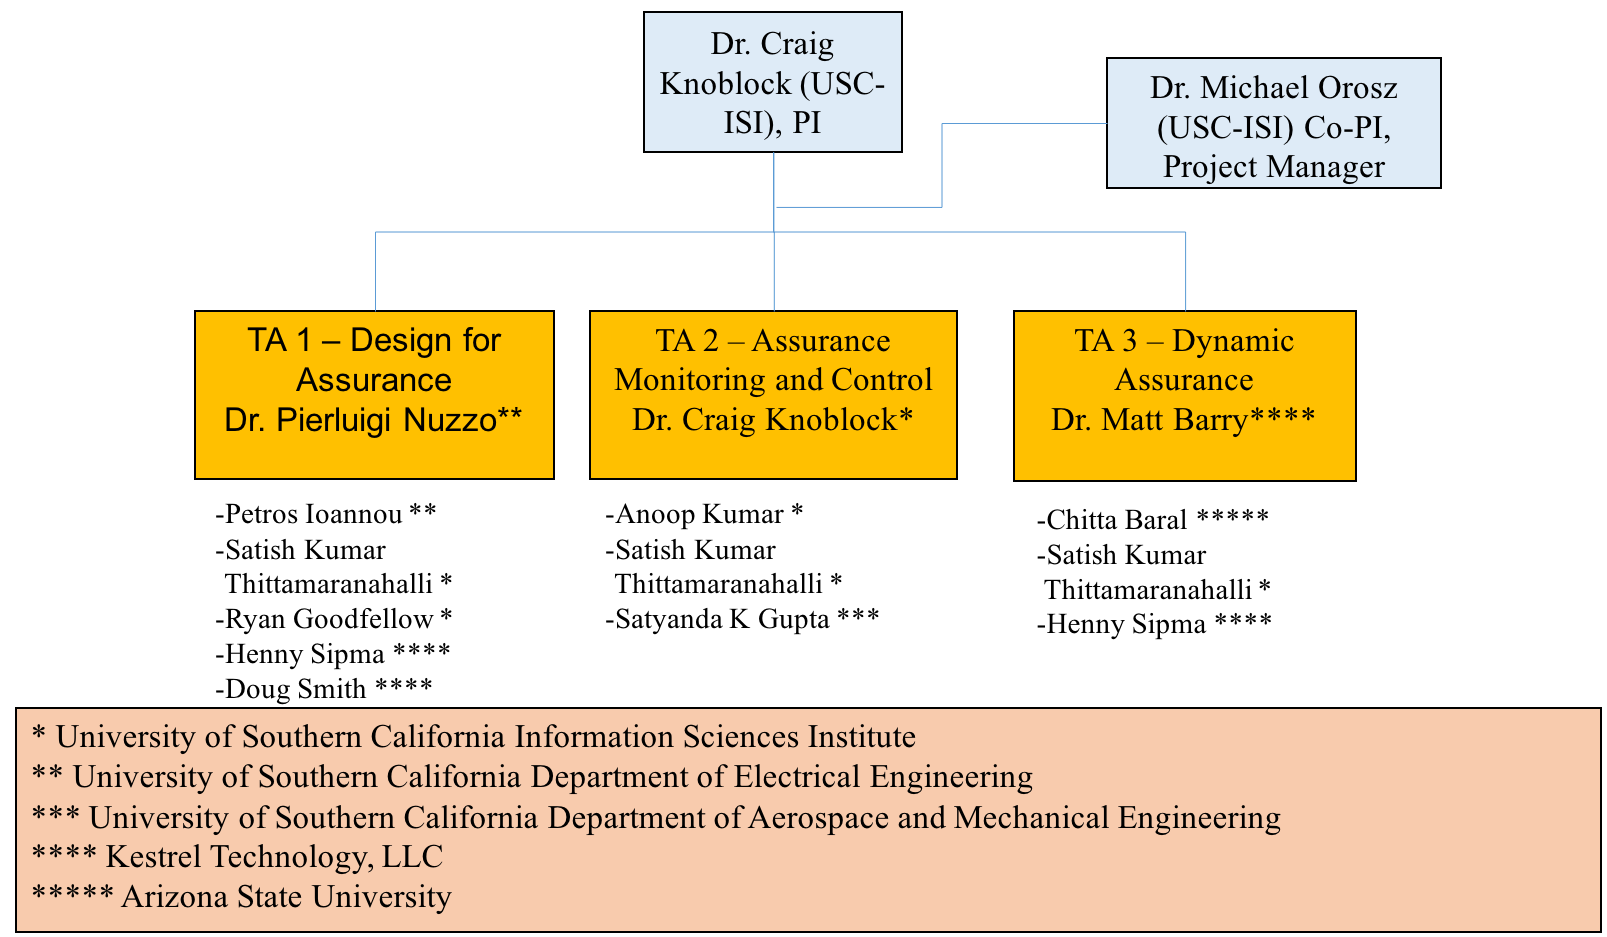
\includegraphics[width=6.0in]{./org-chart2.png}
\caption{\small Organization Chart}
\label{fig:org_chart}
\end{figure}

Coordination: To maximize collaboration and reduce risk to project failure from lack of communication and technical exchange, we plan to employ a wide variety of working styles and communication/coordination so that all can contribute.  At the core of our project will be regularly scheduled meetings bridging the diversely distributed team (Table~\ref{fig:Collaboration_Table}).  These meetings will address project status, identify challenges, implement risk mitigation strategies and participate in technology exchanges and system integration efforts (when appropriate)

\begin{table}[ht]
\caption{\small Project Meetings and Events}
  \centering
  {\footnotesize
\begin{tabular}{|m{3.15in}|m{3in}|} 
\hline
\textbf{Meeting} & \textbf{Frequency} 
\\\hline
Conference calls among investigators (discuss project status, address concerns and project risks) & Weekly
\\
\hline
Technical exchange and coordination meetings using Bluejeans or another videoconference technology & At least twice a month and more frequently as needed
  \\ 
\hline
Face-to-Face meetings (prior to P/I and demonstration meetings) & Every 3 to 6 months and more frequently (especially at the beginning of the project) as needed
 \\\cline{1-2}

\hline
\end{tabular}
}
\label{fig:Collaboration_Table}
\end{table}

\begin{table}[tbhp]
\caption{\small Key Project Team Member Responsibilities}
  \centering
  {\footnotesize
\begin{tabular}{| m{.75in} | m{3.9in}| m{1.5in}|} 
\hline
\textbf{Key Member} & \textbf{Responsibilities} & \textbf{Tasks} 
\\\hline
Dr.\ Craig Knoblock  & Principal Investigator responsible for project, leads TA 2 – Assurance Monitoring and Control.  Will lead the overall project and lead the TA2 team.  Served as the PI on many DARPA projects and has sucessfully led many large teams.    Effort on project:  25\% &
1.1.6, 1.2.2 1.2.3, 1.2.4, 1.3.4, 1.4.1, 
2.1.6, 2.2.2 2.2.3, 2.2.4, 2.3.4, 2.4.1, 
3.1.6, 3.2.2, 3.2.3, 3.2.4, 3.3.4, 3.4.1
\\
\hline
Dr.\ Michael Orosz & Co-Principal Investigator responsible managing the day-to-day operations of the project, assist technical teams as needed, coordinate with TA4 teams.    Has led many large complex multi-disciplined/multi-organizational projects in academic and industry environments.  Effort on project: 50\%
& 1.1.6, 2.1.6, 3.1.6, 1.4.1, 2.4.1, 3.4.1
  \\ 
\hline
Dr.\ Pierluigi Nuzzo 
& 
Co-Principal Investigator.  Leads the TA 1 - Design for Assurance team and conducts research on the formal methods for the design of the TA1 system.  Research experience on methodologies and tools for the design of cyber-physical systems; contracts, interfaces, and compositional methods for embedded system design; the application of automated formal methods and optimization theory to problems in embedded and cyber-physical systems.  Effort on project: 2 months/year (16.6\%)
& 
1.1.1, 2.1.1, 3.1.1 \\
\hline
Dr.\ Matthew Barry
& 
Key personnel.  Leads the TA 3 – Dynamic Assurance.   He will conduct the research on the dynamic assurance case language editors and parsers, the run-time system, and system integrations. Effort on project:  66\%
& 
1.3.2, 2.3.2, 3.3.2\\
\hline
Dr.\ Chitta Baral
& 
Key personnel responsible for learning assurance rules, supporting assurance rules with uncertainty and improving solver speed.  Expertise on ASP solvers, which will be used to reason about the assurance cases. Effort on project: 20\%
& 
1.3.1, 2.3.1, 3.3.1 \\
\hline
Dr.\ Doug Smith 
& 
Key personnel will support formal methods aspects of TA1, and lead the effort on abstract refinement. Expertise in field of automated correct-by-construction program generation.    Effort on project: 40\%
& 
1.1.5, 2.1.5, 3.1.5 \\
\hline
Dr.\ Henny Sipma
& 
Key personnel who will support the program verification tasks under TA1.  Will lead the effort on program verification.   Effort on project:  45\%
& 
1.1.5, 2.1.5, 3.1.5, 1.3.2, 2.3.2, 3.3.2 \\
\hline
Dr.\ Petros Ioannou
& 
Key personnel responsible providing and extending the assurance test bed, which will be available at the start of the project for autonomous vehicles.   Effort on project: 1 month/year (8.3\%)
& 
1.1.2, 2.1.2 (optional), 3.1.2 (optional)
\\
\hline
Dr.\ Satyandra Kumar Gupta
& 
Key Personnel providing autonomous command and control expertise to the TA-2 team.   Will lead the research on safety aware learning on TA2.   Past research on physics-aware decision making to facilitate automation.  Effort on project: 1 month/year (8.3\%)
& 
1.2.1, 2.2.1, 3.2.1 \\
\hline
Dr.\ Anoop Kumar 
& 
Key personnel providing support to the TA 2 project team.  Will lead the research on monitoring \& control and detecting distribution shifts.  Effort on project: 50\%
& 
1.2.1, 1.2.2, 1.2.3, 1.2.4, 2.2.1, 2.2.2, 2.2.3, 2.2.4, 3.2.1, 3.2.2, 3.2.3, 3.2.4\\
\hline
Dr.\ Satish Thittamaranahalli
& 
Key personnel developing scalable algorithms for TA1, TA2, and TA3 project teams.  Has extensive experience on scalable algorithm design, machine learning, and constraint reasoning.  Effort on project: 50\%
& 
1.2.1, 1.2.2, 1.2.3, 1.2.4, 2.2.1, 2.2.2, 2.2.3, 2.2.4, 3.2.1, 3.2.2, 3.2.3, 3.2.4, 1.1.4, 2.1.4, 3.1.4 \\
\hline
Dr.\ Ryan Goodfellow
& 
Key personnel providing support to the TA-1 project. Will lead the research on simulation-based testing.  Has extensive experience on simulation-based testing.  Effort on project:  30\%
& 
1.1.3, 2.1.3, 3.1.3 \\

\cline{1-2}

\hline
\end{tabular}
}
\label{fig:Table_Mgmt}
\end{table}



\newpage
\section{Personnel, Qualifications and Commitment}

{\bf Dr.\ Craig Knoblock}, the PI on this effort, is a Research Professor of both Computer Science and Spatial Sciences at the University of Southern California (USC) and Director of the Intelligent Systems Division at the USC Information Sciences Institute.   He received his Ph.D. from Carnegie Mellon University in computer science. 
%His research focuses on techniques for describing, acquiring, and exploiting the semantics of data.  
In previous projects he has worked on developing  scalable approaches to execution monitoring, accurate detection of sensor failures, and   automatic modeling and reconstruction of sensors.  He has published more than 300 journal articles, book chapters, and conference papers on these topics.  Dr. Knoblock is a Fellow of the Association for the Advancement of Artificial Intelligence (AAAI), a Distinguished Scientist of the Association of Computing Machinery (ACM), a Senior Member of IEEE, past President and Trustee of the International Joint Conference on Artificial Intelligence.
%and winner of the 2014 Robert S. Engelmore Award.  

{\bf Dr.\ Michael Orosz}, a Co-PI on this effort, is a Research Associate Professor of Civil and Environmental Engineering at the University of Southern California (USC) and Research Director of the Decision Systems Group at the USC Information Sciences Institute.  Dr. Orosz has over 30 years’ experience in commercial and government software development, basic and applied research, project management, academic research and has developed and deployed several commercially successful products.  His research interests are in machine learning and decision analytics as applied to intelligence analysis and autonomous command and control such as smart building controls.    Dr. Orosz has extensive experience in managing large complex multi-disciplined/multi-teamed research projects. %funded by DARPA, DHS, DoD, DoE, Industry, NASA, NRO, NSA and ONR.   
He received his Ph.D. in computer science from the University of California, Los Angeles.

{\bf Dr.\ Pierluigi Nuzzo}, a Co-PI on this project, is an Assistant Professor in the Department of Electrical Engineering at the University of Southern California. He received the Ph.D. in Electrical Engineering and Computer Sciences from the University of California at Berkeley. 
%in 2015, and the Laurea degree (MS) in electrical engineering (summa cum laude) from the University of Pisa, Italy, and the Sant'Anna School of Advanced Studies, Pisa, Italy.
%
%He has four years of research experience in analog and mixed signal circuit design as a researcher at IMEC, Leuven, Belgium, and over 10 years experience in design methodologies and tools for mixed-signal integrated circuits and cyber-physical systems, as a researcher at the University of Pisa, IMEC, UC Berkeley, and USC. 
His research interests
include: methodologies and tools for cyber-physical system and mixed-signal
system design; contracts, interfaces and compositional methods for embedded
system design; the application of formal methods and optimization theory to problems in embedded and cyber-physical systems and electronic design automation. 
%
Prof. Nuzzo received %First Place in the operational category and Best Overall
%Submission in the 2006 DAC/ISSCC Design Competition, 
a Marie Curie Fellowship
from the European Union in 2006, 
the University of California at Berkeley EECS
departmental fellowship in 2008, 
%the University of California at Berkeley Outstanding Graduate Student Instructor Award in 2013, 
the IBM Ph.D.
Fellowship in 2012 and 2014, 
%the Best Paper Award from the International Conference on Cyber-Physical Systems (ICCPS) in 2016, 
and the David J.~Sakrison Memorial Prize in 2016 for his doctoral research. 
%He is an author of 1 patent and over 60 publications.

{\bf Dr.\ Satyandra K. Gupta} is Smith International Professor in the Department of Aerospace and Mechanical Engineering at the University of Southern California. %Prior to joining the University of Southern California, he was a Professor in the Department of Mechanical Engineering and the Institute for Systems Research at the University of Maryland. He was the founding director of the Maryland Robotics Center and the Advanced Manufacturing Laboratory at the University of Maryland. 
He served as a program director for the National Robotics Initiative at the National Science Foundation from September 2012 to September 2014.  Dr. Gupta's interest is in the area of physics-aware decision making to facilitate automation. He has published more than 300 technical articles. He is a fellow of the American Society of Mechanical Engineers (ASME) and editor of ASME Journal of Computing and Information Science in Engineering. Dr. Gupta has received the Young Investigator Award from the Office of Naval Research in 2000, CAREER Award from the National Science Foundation in 2001, Presidential Early Career Award for Scientists and Engineers (PECASE) in 2001, Invention of the Year Award at the University of Maryland in 2007, Kos Ishii-Toshiba Award from ASME in 2011, and Excellence in Research Award from ASME in 2013.%, and Distinguished Alumnus Award from Indian Institute of Technology, Roorkee in 2014. %He has also received seven best paper awards at conferences.

{\bf Ryan Goodfellow} is a computer scientist at ISI working in combined cyber physical simulation and emulation platform development. His formal background is in simulation algorithms and modeling techniques using differential-algebraic equations (DAE). He has applied this knowledge in the CPS space by integrating DAE modeling languages and simulation engines with network testbeds to create comprehensive scientific experimentation platforms for cyber-physical systems. These experimentation platforms have been used in the power grid research space. %Ryan is a lead developer on the Deter network testbed, with a strong background in networked and distributed systems engineering. %He is also a combat veteran, serving as a non-commissioned officer and SIGINT team lead for a multi-functional intelligence team in Afghanistan.

{\bf Dr.\ Petros Ioannou} is a Professor in the Department of Electrical Engineering, Director of the Center for Advanced Transportation Technologies and Associate Director for Research for the DOT supported University Transportation Center at USC. He received his MS and PhD from the University of Illinois at Urbana Champaign in Mechanical and Electrical Engineering, respectively. His research interests are in robust adaptive control, vehicle dynamics and control, human factors and safety, automated vehicles, nonlinear systems and Intelligent transportation Systems.  He received the 2016 IEEE Transportation Technologies field award and the 2016 IEEE Control system society Transition to Practice Award. He is a Fellow of IEEE, IFAC and IET and author/coauthor of 8 books and over 400 papers.

{\bf Dr.\ Matthew Barry} will serve as lead for the TA3 tasks. %He will implement the dynamic assurance case language editors and parsers, the run-time system, and system integrations.  He will implement the assurance case arguments and the API for updating argument structure and content.  
Dr. Barry currently is CEO at Kestrel Technology LLC, and previously spent 20 years in NASA space mission operations at the Jet Propulsion Lab and Johnson Space Center.  At NASA Headquarters he led the introduction of dependability case requirements and plans for flight computing systems in upcoming manned space exploration missions, as well as the development of Agency-level software-related safety-critical control system requirements.  He recently served as a Principal Investigator on DHS/Cyber S\&T STAMP (Static Tool Analysis Modernization Program), DARPA CSFV (Crowd Sourced Formal Verification), three NASA Aeronautics R\&D projects, and the AFRL-sponsored Static Analysis of Numerical Algorithms project.  Dr. Barry earned BSME, MS, and PhD degrees in mechanical engineering, and an MBA degree, from Rice University.  

{\bf Dr.\ Henny Sipma} will support the program verification tasks under TA1.  %She is the key person behind the company's {\em KT Advance\/} and {\em KT Transferal\/} static analysis products, and the designer and programmer of the company's core {\em CodeHawk\/} abstract interpretation engine. 
Dr. Sipma currently is the CTO at Kestrel Technology LLC.  She has spent the past 10 years with Kestrel Technology as a static analysis expert; previously developed and taught static analysis techniques as senior research associate at Stanford University for eight years; and developed industrial process controls as an senior systems analyst at Shell.  She has been Principal Investigator or company lead on several recent R\&D projects for Federal agencies, including two projects under the IARPA STONESOUP (Securely Taking On New Executable Software of Uncertain Provenance) program; the DHS Cyber S\&T Gold Standard project; and the DARPA-sponsored STAC (Space-Time Analysis for Cybersecurity) and MUSE (Mining and Understanding Software Enclaves) programs.  Dr. Sipma earned 
%a BS degree in chemistry and an MS degree in chemical engineering at the University of Groningen in The Netherlands, and 
MS and PhD degrees in computer science from Stanford University.  

{\bf Dr.\ Douglas R.\ Smith} will support formal methods aspects of TA1, including the enforcement of safety properties and the generation of monitors.  He is President of Kestrel Technology LLC and Principal Scientist at Kestrel Institute.  He is a Fellow of the American Association of Artificial Intelligence (AAAI) and an ASE Fellow (Automated Software Engineering).  From 1986 to 2000, he taught an advanced graduate course on correct-by-construction software development at Stanford.  
%Dr. Smith has led the development of a series of software synthesis systems, including KIDS (Kestrel Interactive Development System), Specware, Designware, and Planware. 
%Applications domains have included a variety of complex high-performance planners and schedulers for the US Air Force.  He leads current projects on the generation of air mission plans and cyberoperations.  
Other recent projects focused on automated policy enforcement \cite{SmithD0703,SmithD08}, synthesis of secure network protocol codes, and the synthesis of high-performance constraint-solvers\cite{SmithD08c,SmithD13}.  Dr. Smith has over 30 years experience in the field of automated correct-by-construction program generation and has published over 100 papers. He has one patent.  He received the Ph.D. in Computer Science from Duke University% in 1979.  

{\bf Dr. Chitta Baral} is a Professor in the Department of Computer Science and Engineering at Arizona State University. He will support the TA3 efforts on Learning assurance rules, supporting assurance rules with uncertainty and improving solver speed. Dr. Baral has expertise in various aspects of autonomy and Artificial Intelligence. 
He wrote the first book on answer set programming (published by Cambridge University Press) the formal language behind our assurance rules. Some of his other works relevant to this proposal are: goal specification for autonomous systems, automatic construction of control rules for autonomous systems that satisfy given goals, combining machine learning with reasoning in various contexts, including image understanding. %He is the President of KR Inc. He is an associate editor of AIJ and has been an associate editor of JAIR.

{\bf Dr.\ Satish Kumar Thittamaranahalli (T. K. Satish Kumar)} leads the Collaboratory for Algorithmic Techniques and Artificial Intelligence (CATAI) at USC's Information Sciences Institute. He has published over 60 papers on numerous topics in Artificial Intelligence spanning such diverse areas as Constraint Reasoning, Planning and Scheduling, Probabilistic Reasoning, Robotics, Combinatorial Optimization, Approximation and Randomization, Heuristic Search, Model-Based Reasoning, Knowledge Representation and Spatio-Temporal Reasoning. %He %has served on the Program Committees of many international conferences in Artificial Intelligence
He and is a winner of the 2016 Best Robotics Paper Award and the 2005 Best Student Paper Award from the International Conference on Automated Planning and Scheduling. 
Dr. Kumar received his PhD in Computer Science from Stanford University. %In the past, he has also been a Visiting Student at the NASA Ames Research Center, a Postdoctoral Research Scholar at the University of California, Berkeley, a Research Scientist at the Institute for Human and Machine Cognition, a Visiting Assistant Professor at the University of West Florida, and a Senior Research and Development Scientist at Mission Critical Technologies.

\textbf{Dr.\ Anoop Kumar} is a senior computer scientist at USC ISI and has broad expertise in machine learning, statistical modeling, and software engineering.  Dr.\ Kumar is the technical lead on the DARPA RSPACE program and has played a vital role in developing a system that fuses air operations data from multiple sources, maintains world state, and issues warnings. Previously, he led the research and development of the BBN’s election forecasting system for the IARPA OSI program. %Dr.\ Kumar played a significant role in the DARPA DEFT program by developing a model to support integration of output from multiple NLP algorithms. He has contributed at the development to management levels on government research contracts and commercial projects. 
Dr.\ Kumar helped design and develop BBN's commercially available, hosted speech and medical transcription services offering. 

\begin{table}[!tbh]
\begin{footnotesize}
\vspace{-0.1in}

\begin{tabular}{lll}
\begin{tabular}[t]{|l|@{}c@{}|@{}c@{}|@{}c@{}|@{}c@{}|} \hline
Project & Status & \multicolumn{3}{ c| }{Hours} \\ \cline{3-5}
& & P1 & P2 & P3 \\ \hline



\multicolumn{5}{ |c| }{ \textbf{Craig Knoblock} } \\ \cline{1-5}
Safeguard & Pro & 770 & 641 & 641 \\ \cline{1-5}
ELICIT & Cur & 308 & 256 & 120 \\ \cline{1-5}
WTNIC & Cur & 11 & 0 & 0 \\ \cline{1-5}
EFFECT & Cur & 641 & 107 & 0 \\ \cline{1-5}
LinkedMaps & Cur & 203 & 25 & 0 \\ \cline{1-5}
PRINCESS & Cur & 608 & 96 & 0 \\ \cline{1-5}
SCHARP & Cur & 481 & 54 & 0 \\ \cline{1-5}
MINT & Pen & 650 & 534 & 285 \\ \cline{1-5}

\multicolumn{5}{ |c| }{ \textbf{Michael Orosz} } \\ \cline{1-5}
Safeguard & Pro & 1560 & 1300 & 1300  \\ \cline{1-5}
SMC/SY & Cur & 1803 & 0 & 0  \\ \cline{1-5}

\multicolumn{5}{ |c| }{ \textbf{Matthew Barry} } \\ \cline{1-5}
Safeguard & Pro & 2078 & 1690 & 1554 \\ \cline{1-5}
Starlite & Cur & 1840 & 1692 & 0 \\ \cline{1-5}



\multicolumn{5}{ |c| }{ \textbf{Anoop Kumar} } \\ \cline{1-5}
Safeguard & Pro & 1560 & 1300 & 1300 \\ \cline{1-5}

\end{tabular}
&
\begin{tabular}[t]{|l|@{}c@{}|@{}c@{}|@{}c@{}|@{}c@{}|} \hline
Project & Status & \multicolumn{3}{ c| }{Hours} \\ \cline{3-5}
& & P1 & P2 & P3 \\ \hline

\multicolumn{5}{ |c| }{ \textbf{Pierluigi Nuzzo} } \\ \cline{1-5}
Safeguard & Pro & 520 & 433 & 433  \\ \cline{1-5}
Mirage & Cur & 433 & 0 & 0  \\ \cline{1-5}

\multicolumn{5}{ |c| }{ \textbf{Satyandra Gupta} } \\ \cline{1-5}
Safeguard & Pro & 260 & 217 & 217 \\ \cline{1-5}
Human   & Cur & 22 & 0 & 0 \\ \cline{1-5}
Vehicles & Cur & 36 & 0 & 0 \\ \cline{1-5}
Robot & Cur & 116 & 0 & 0 \\ \cline{1-5}
Assembly & Cur & 33 & 0 & 0 \\ \cline{1-5}
Solar & Cur & 4 & 0 & 0 \\ \cline{1-5}

\multicolumn{5}{ |c| }{ \textbf{Petros Ioannou} } \\ \cline{1-5}
Safeguard & Pro & 260 & 217 & 217 \\ \cline{1-5}
CPS & Cur & 130 & 0 & 0 \\ \cline{1-5}

\multicolumn{5}{ |c| }{ \textbf{Ryan Goodfellow} } \\ \cline{1-5}
Safeguard & Pro & 936 & 780 & 780 \\ \cline{1-5}
STEAM & Cur & 416 & 0 & 0 \\ \cline{1-5}


\end{tabular}
&
\begin{tabular}[t]{|l|@{}c@{}|@{}c@{}|@{}c@{}|@{}c@{}|} \hline
Project & Status & \multicolumn{3}{ c| }{Hours} \\ \cline{3-5}
& & P1 & P2 & P3 \\ \hline

\multicolumn{5}{ |c| }{ \textbf{Chitta Baral} } \\ \cline{1-5}
Safeguard & Pro & 659 & 485 & 485 \\ \cline{1-5}
PostdocBP & Cur & 176 & 0 & 0 \\ \cline{1-5}
Languages & Pen & 528 & 264 & 264 \\ \cline{1-5}
CAREER & Pen & 88 & 44 & 44 \\ \cline{1-5}
CHS & Pen & 510 & 255 & 0 \\ \cline{1-5}

\multicolumn{5}{ |c| }{ \textbf{Doug Smith} } \\ \cline{1-5}
Safeguard & Pro & 1222 & 984 & 840 \\ \cline{1-5}
RSPACE & Cur & 342 & 0 & 0 \\ 
\cline{1-5}
PLANX & Cur & 154 & 0 & 0 \\ 
\cline{1-5}
HACCS & Pen & 923 & 769 & 769 \\ 
\cline{1-5}

\multicolumn{5}{ |c| }{ \textbf{Henny Sipma} } \\ \cline{1-5}
Safeguard & Pro & 1372 & 962 & 840 \\ \cline{1-5}
STAC & Cur & 797 & 0 & 0 \\ \cline{1-5}

\multicolumn{5}{ |c| }{ \textbf{Satish Thittamaranahalli} } \\ \cline{1-5}
Safeguard & Pro & 1560 & 1300 & 1300 \\ \cline{1-5}
MapF & Cur & 103 & 103 & 0 \\ \cline{1-5}

\end{tabular}
\end{tabular}

\end{footnotesize}
\caption{Individual commitments of key personnel}
\label{tab:Commitments}
\vspace{-0.2in}
\end{table}

\clearpage
\newpage
\section{Capabilities}


%\subsection{University of Southern California}
USC has strengths in number of areas that are closely related to the proposed work:
\begin{itemize}[itemsep=0pt,leftmargin=*]
\item Dr.\ Nuzzo 
%has over 10-year research experience in embedded system design, from mixed-signal chip design (analog-to-digital converters, frequency synthesizers, software-defined radio), to methodologies and tools for mixed-signal integrated circuits and Cyber-Physical Systems (CPSs), and the application of formal methods and optimization theory to problems in embedded and cyber-physical systems and electronic design automation.  
%His doctoral work 
has done extensive research on contracts and compositional methods for heterogeneous system design and design space exploration, with application to aircraft electric power systems and environmental control systems. His work has helped transition rigorous system design foundations, innovative design methodologies, and new systems engineering paradigms to industry (IBM, United Technologies). 
\item Dr.\ Satyandra K. Gupta has worked on autonomous surface vehicles, autonomous ground vehicles for operation on rugged terrains, and autonomous flapping wing aerial vehicles.   His group has developed a hierarchal decision making approach for realizing autonomous systems. 
%This approach combines task planning and assignment, deliberative trajectory planning, reactive collision avoidance behaviors, and trajectory tracking control layers. 
His group has also developed new methods for learning reactive behaviors in adversarial environments and COLREGS compliant trajectory planning. \item Dr.\ Knoblock has developed methods that learn the relationships between sensors to both identify failures and changes in sensor and reconstruct those sensors, providing estimates of the accuracy of the reconstructed sensors.  
\item Ryan Goodfellow has extensive experience in simulation based testing through high-fidelity CPS testbed environment development and operation, using the Deter network testbed as the core which has supported several large scale government projects from a variety of agencies and thousands of users. %we have developed sophisticated CPS experiments under programs such as NFS RIPS, NIST SmartCities and the DHS Cybersecurity showcase.
\item Dr.\ Ioannou %helped  design and implement adaptive cruise control systems in collaboration with Ford Motor Company, which was commercialized four years before any other company. He 
worked on several DOT funded projects on automated vehicles and intelligent highway systems where he demonstrated his vehicle control designs for safety and performance on actual automated vehicles in test trucks and I-15 highway.
\item Drs.\ Knoblock, Kumar, and Thittamaranahalli have developed highly scalable approaches for monitoring message traffic to identify potential problems and issue warnings and alerts. 
\item Dr. Thittamaranahalli has developed state-of-the-art methods for efficiently solving large-scale search and optimization problems. %These techniques will be applicable in TA2 for safety-aware learning and planning, in TA2 for assurance monitoring and control, and in TA3 for dynamic assessment of assurance cases.

\end{itemize}
%\subsection{Kestrel Technology LLC}

Kestrel Technology's strength is in program analysis, specifically static analysis of both source and binary targets.  The company performs applied R\&D and product development for a variety of static analysis applications  pivoting primarily on the abstract interpretation technique.  The company recently initiated development of program analysis applications using logical equivalence techniques. As a provider of verification evidence in the form of mathematical proofs, the company also has expertise in the design and development of assurance case arguments for high-integrity systems using such evidence. %The company is engaged in a partnership with Wind River Systems to develop program analysis tools for its embedded system developers.  Many of Wind River's customers must develop their products under safety and certification standards, including those using safety cases.  

   

%\subsection{Arizona State University}
Chitta Baral at Arizona State University has developed various software to learn assurance rules and various ASP solvers, which he has made available as open-source.

Most of the software carried forward for implementation or derivation is open source.  The single exception is Kestrel Technology's {\it KT Advance\/} static analysis tool (TA1), in particular the abstract interpretation engine therein, which is company proprietary and is US EAR export-controlled.   
%Owing to mixed funding for the development of that technology 
We will continue to provide the Federal government a restricted use license for that particular item.

There are no specialized facilities, data, or GFE required for this effort. 

\include{sow}
\include{milestones}

% \section{Level of Effort by Task \textcolor{red}{[Mike/Lisa - 1 pages]}}

% \textcolor{blue}{
% \begin{itemize}
% \item Will be a separate spreadsheet
% \item
% \end{itemize}
% }

\include{appendix_a}

%\section{Appendix B \textcolor{red}{[No Page Count]}}

\section{References}
\bibliographystyle{acm} 
\bibliography{TA3/ta3,TA2/ta2,TA1/ta1}
\end{document}
\clearpage
\newpage


\section{Management Plan}


The Principal Investigator for this effort is Dr. Craig Knoblock who is responsible for all aspects of the effort, will coordinate the parallel team efforts, and will ensure high levels of performance from individual team members.  The Co-P/I, Dr. Michael Orosz, will provide project management and will assist all performers in the execution of the project.    The project team is divided into three working groups (Figure~\ref{fig:org_chart}) corresponding to Technical Areas 1-3, however, members of each team contribute across all project activities.   Table~\ref{fig:Table_Mgmt} defines the major contributions of each project team member to the project tasks.

\begin{figure}[tbhp]
%\vspace{-25pt}
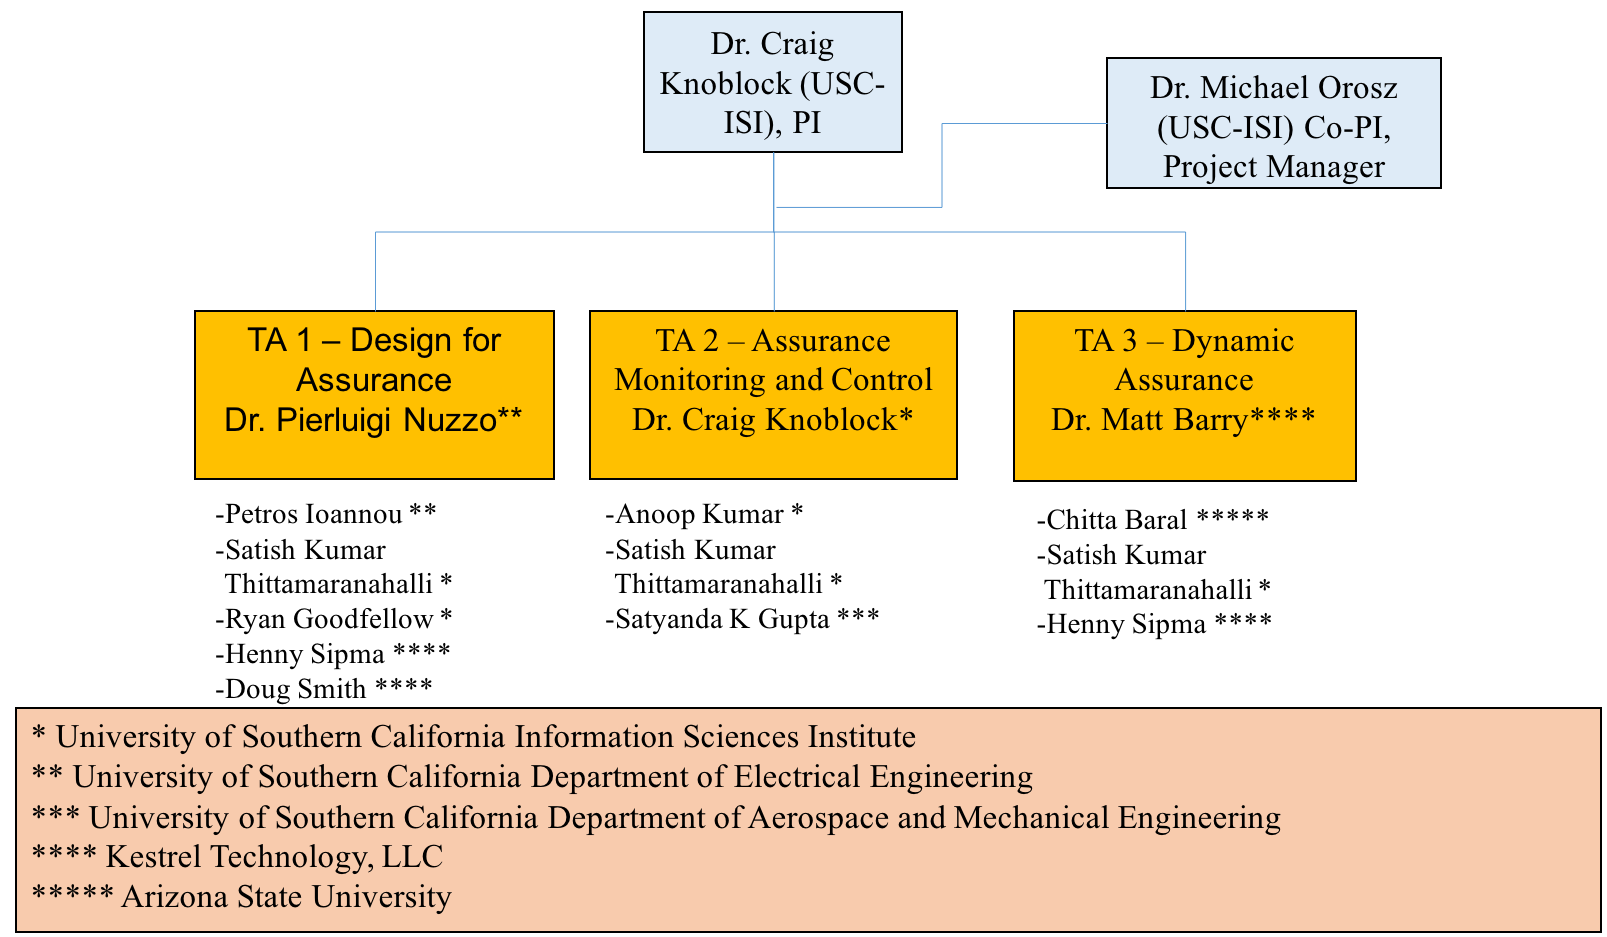
\includegraphics[width=6.0in]{./org-chart2.png}
\caption{\small Organization Chart}
\label{fig:org_chart}
\end{figure}

Coordination: To maximize collaboration and reduce risk to project failure from lack of communication and technical exchange, we plan to employ a wide variety of working styles and communication/coordination so that all can contribute.  At the core of our project will be regularly scheduled meetings bridging the diversely distributed team (Table~\ref{fig:Collaboration_Table}).  These meetings will address project status, identify challenges, implement risk mitigation strategies and participate in technology exchanges and system integration efforts (when appropriate)

\begin{table}[ht]
\caption{\small Project Meetings and Events}
  \centering
  {\footnotesize
\begin{tabular}{|m{3.15in}|m{3in}|} 
\hline
\textbf{Meeting} & \textbf{Frequency} 
\\\hline
Conference calls among investigators (discuss project status, address concerns and project risks) & Weekly
\\
\hline
Technical exchange and coordination meetings using Bluejeans or another videoconference technology & At least twice a month and more frequently as needed
  \\ 
\hline
Face-to-Face meetings (prior to P/I and demonstration meetings) & Every 3 to 6 months and more frequently (especially at the beginning of the project) as needed
 \\\cline{1-2}

\hline
\end{tabular}
}
\label{fig:Collaboration_Table}
\end{table}

\begin{table}[tbhp]
\caption{\small Key Project Team Member Responsibilities}
  \centering
  {\footnotesize
\begin{tabular}{| m{.75in} | m{3.9in}| m{1.5in}|} 
\hline
\textbf{Key Member} & \textbf{Responsibilities} & \textbf{Tasks} 
\\\hline
Dr.\ Craig Knoblock  & Principal Investigator responsible for project, leads TA 2 – Assurance Monitoring and Control.  Will lead the overall project and lead the TA2 team.  Served as the PI on many DARPA projects and has sucessfully led many large teams.    Effort on project:  25\% &
1.1.6, 1.2.2 1.2.3, 1.2.4, 1.3.4, 1.4.1, 
2.1.6, 2.2.2 2.2.3, 2.2.4, 2.3.4, 2.4.1, 
3.1.6, 3.2.2, 3.2.3, 3.2.4, 3.3.4, 3.4.1
\\
\hline
Dr.\ Michael Orosz & Co-Principal Investigator responsible managing the day-to-day operations of the project, assist technical teams as needed, coordinate with TA4 teams.    Has led many large complex multi-disciplined/multi-organizational projects in academic and industry environments.  Effort on project: 50\%
& 1.1.6, 2.1.6, 3.1.6, 1.4.1, 2.4.1, 3.4.1
  \\ 
\hline
Dr.\ Pierluigi Nuzzo 
& 
Co-Principal Investigator.  Leads the TA 1 - Design for Assurance team and conducts research on the formal methods for the design of the TA1 system.  Research experience on methodologies and tools for the design of cyber-physical systems; contracts, interfaces, and compositional methods for embedded system design; the application of automated formal methods and optimization theory to problems in embedded and cyber-physical systems.  Effort on project: 2 months/year (16.6\%)
& 
1.1.1, 2.1.1, 3.1.1 \\
\hline
Dr.\ Matthew Barry
& 
Key personnel.  Leads the TA 3 – Dynamic Assurance.   He will conduct the research on the dynamic assurance case language editors and parsers, the run-time system, and system integrations. Effort on project:  66\%
& 
1.3.2, 2.3.2, 3.3.2\\
\hline
Dr.\ Chitta Baral
& 
Key personnel responsible for learning assurance rules, supporting assurance rules with uncertainty and improving solver speed.  Expertise on ASP solvers, which will be used to reason about the assurance cases. Effort on project: 20\%
& 
1.3.1, 2.3.1, 3.3.1 \\
\hline
Dr.\ Doug Smith 
& 
Key personnel will support formal methods aspects of TA1, and lead the effort on abstract refinement. Expertise in field of automated correct-by-construction program generation.    Effort on project: 40\%
& 
1.1.5, 2.1.5, 3.1.5 \\
\hline
Dr.\ Henny Sipma
& 
Key personnel who will support the program verification tasks under TA1.  Will lead the effort on program verification.   Effort on project:  45\%
& 
1.1.5, 2.1.5, 3.1.5, 1.3.2, 2.3.2, 3.3.2 \\
\hline
Dr.\ Petros Ioannou
& 
Key personnel responsible providing and extending the assurance test bed, which will be available at the start of the project for autonomous vehicles.   Effort on project: 1 month/year (8.3\%)
& 
1.1.2, 2.1.2 (optional), 3.1.2 (optional)
\\
\hline
Dr.\ Satyandra Kumar Gupta
& 
Key Personnel providing autonomous command and control expertise to the TA-2 team.   Will lead the research on safety aware learning on TA2.   Past research on physics-aware decision making to facilitate automation.  Effort on project: 1 month/year (8.3\%)
& 
1.2.1, 2.2.1, 3.2.1 \\
\hline
Dr.\ Anoop Kumar 
& 
Key personnel providing support to the TA 2 project team.  Will lead the research on monitoring \& control and detecting distribution shifts.  Effort on project: 50\%
& 
1.2.1, 1.2.2, 1.2.3, 1.2.4, 2.2.1, 2.2.2, 2.2.3, 2.2.4, 3.2.1, 3.2.2, 3.2.3, 3.2.4\\
\hline
Dr.\ Satish Thittamaranahalli
& 
Key personnel developing scalable algorithms for TA1, TA2, and TA3 project teams.  Has extensive experience on scalable algorithm design, machine learning, and constraint reasoning.  Effort on project: 50\%
& 
1.2.1, 1.2.2, 1.2.3, 1.2.4, 2.2.1, 2.2.2, 2.2.3, 2.2.4, 3.2.1, 3.2.2, 3.2.3, 3.2.4, 1.1.4, 2.1.4, 3.1.4 \\
\hline
Dr.\ Ryan Goodfellow
& 
Key personnel providing support to the TA-1 project. Will lead the research on simulation-based testing.  Has extensive experience on simulation-based testing.  Effort on project:  30\%
& 
1.1.3, 2.1.3, 3.1.3 \\

\cline{1-2}

\hline
\end{tabular}
}
\label{fig:Table_Mgmt}
\end{table}



\newpage
\section{Personnel, Qualifications and Commitment}

{\bf Dr.\ Craig Knoblock}, the PI on this effort, is a Research Professor of both Computer Science and Spatial Sciences at the University of Southern California (USC) and Director of the Intelligent Systems Division at the USC Information Sciences Institute.   He received his Ph.D. from Carnegie Mellon University in computer science. 
%His research focuses on techniques for describing, acquiring, and exploiting the semantics of data.  
In previous projects he has worked on developing  scalable approaches to execution monitoring, accurate detection of sensor failures, and   automatic modeling and reconstruction of sensors.  He has published more than 300 journal articles, book chapters, and conference papers on these topics.  Dr. Knoblock is a Fellow of the Association for the Advancement of Artificial Intelligence (AAAI), a Distinguished Scientist of the Association of Computing Machinery (ACM), a Senior Member of IEEE, past President and Trustee of the International Joint Conference on Artificial Intelligence.
%and winner of the 2014 Robert S. Engelmore Award.  

{\bf Dr.\ Michael Orosz}, a Co-PI on this effort, is a Research Associate Professor of Civil and Environmental Engineering at the University of Southern California (USC) and Research Director of the Decision Systems Group at the USC Information Sciences Institute.  Dr. Orosz has over 30 years’ experience in commercial and government software development, basic and applied research, project management, academic research and has developed and deployed several commercially successful products.  His research interests are in machine learning and decision analytics as applied to intelligence analysis and autonomous command and control such as smart building controls.    Dr. Orosz has extensive experience in managing large complex multi-disciplined/multi-teamed research projects. %funded by DARPA, DHS, DoD, DoE, Industry, NASA, NRO, NSA and ONR.   
He received his Ph.D. in computer science from the University of California, Los Angeles.

{\bf Dr.\ Pierluigi Nuzzo}, a Co-PI on this project, is an Assistant Professor in the Department of Electrical Engineering at the University of Southern California. He received the Ph.D. in Electrical Engineering and Computer Sciences from the University of California at Berkeley. 
%in 2015, and the Laurea degree (MS) in electrical engineering (summa cum laude) from the University of Pisa, Italy, and the Sant'Anna School of Advanced Studies, Pisa, Italy.
%
%He has four years of research experience in analog and mixed signal circuit design as a researcher at IMEC, Leuven, Belgium, and over 10 years experience in design methodologies and tools for mixed-signal integrated circuits and cyber-physical systems, as a researcher at the University of Pisa, IMEC, UC Berkeley, and USC. 
His research interests
include: methodologies and tools for cyber-physical system and mixed-signal
system design; contracts, interfaces and compositional methods for embedded
system design; the application of formal methods and optimization theory to problems in embedded and cyber-physical systems and electronic design automation. 
%
Prof. Nuzzo received %First Place in the operational category and Best Overall
%Submission in the 2006 DAC/ISSCC Design Competition, 
a Marie Curie Fellowship
from the European Union in 2006, 
the University of California at Berkeley EECS
departmental fellowship in 2008, 
%the University of California at Berkeley Outstanding Graduate Student Instructor Award in 2013, 
the IBM Ph.D.
Fellowship in 2012 and 2014, 
%the Best Paper Award from the International Conference on Cyber-Physical Systems (ICCPS) in 2016, 
and the David J.~Sakrison Memorial Prize in 2016 for his doctoral research. 
%He is an author of 1 patent and over 60 publications.

{\bf Dr.\ Satyandra K. Gupta} is Smith International Professor in the Department of Aerospace and Mechanical Engineering at the University of Southern California. %Prior to joining the University of Southern California, he was a Professor in the Department of Mechanical Engineering and the Institute for Systems Research at the University of Maryland. He was the founding director of the Maryland Robotics Center and the Advanced Manufacturing Laboratory at the University of Maryland. 
He served as a program director for the National Robotics Initiative at the National Science Foundation from September 2012 to September 2014.  Dr. Gupta's interest is in the area of physics-aware decision making to facilitate automation. He has published more than 300 technical articles. He is a fellow of the American Society of Mechanical Engineers (ASME) and editor of ASME Journal of Computing and Information Science in Engineering. Dr. Gupta has received the Young Investigator Award from the Office of Naval Research in 2000, CAREER Award from the National Science Foundation in 2001, Presidential Early Career Award for Scientists and Engineers (PECASE) in 2001, Invention of the Year Award at the University of Maryland in 2007, Kos Ishii-Toshiba Award from ASME in 2011, and Excellence in Research Award from ASME in 2013.%, and Distinguished Alumnus Award from Indian Institute of Technology, Roorkee in 2014. %He has also received seven best paper awards at conferences.

{\bf Ryan Goodfellow} is a computer scientist at ISI working in combined cyber physical simulation and emulation platform development. His formal background is in simulation algorithms and modeling techniques using differential-algebraic equations (DAE). He has applied this knowledge in the CPS space by integrating DAE modeling languages and simulation engines with network testbeds to create comprehensive scientific experimentation platforms for cyber-physical systems. These experimentation platforms have been used in the power grid research space. %Ryan is a lead developer on the Deter network testbed, with a strong background in networked and distributed systems engineering. %He is also a combat veteran, serving as a non-commissioned officer and SIGINT team lead for a multi-functional intelligence team in Afghanistan.

{\bf Dr.\ Petros Ioannou} is a Professor in the Department of Electrical Engineering, Director of the Center for Advanced Transportation Technologies and Associate Director for Research for the DOT supported University Transportation Center at USC. He received his MS and PhD from the University of Illinois at Urbana Champaign in Mechanical and Electrical Engineering, respectively. His research interests are in robust adaptive control, vehicle dynamics and control, human factors and safety, automated vehicles, nonlinear systems and Intelligent transportation Systems.  He received the 2016 IEEE Transportation Technologies field award and the 2016 IEEE Control system society Transition to Practice Award. He is a Fellow of IEEE, IFAC and IET and author/coauthor of 8 books and over 400 papers.

{\bf Dr.\ Matthew Barry} will serve as lead for the TA3 tasks. %He will implement the dynamic assurance case language editors and parsers, the run-time system, and system integrations.  He will implement the assurance case arguments and the API for updating argument structure and content.  
Dr. Barry currently is CEO at Kestrel Technology LLC, and previously spent 20 years in NASA space mission operations at the Jet Propulsion Lab and Johnson Space Center.  At NASA Headquarters he led the introduction of dependability case requirements and plans for flight computing systems in upcoming manned space exploration missions, as well as the development of Agency-level software-related safety-critical control system requirements.  He recently served as a Principal Investigator on DHS/Cyber S\&T STAMP (Static Tool Analysis Modernization Program), DARPA CSFV (Crowd Sourced Formal Verification), three NASA Aeronautics R\&D projects, and the AFRL-sponsored Static Analysis of Numerical Algorithms project.  Dr. Barry earned BSME, MS, and PhD degrees in mechanical engineering, and an MBA degree, from Rice University.  

{\bf Dr.\ Henny Sipma} will support the program verification tasks under TA1.  %She is the key person behind the company's {\em KT Advance\/} and {\em KT Transferal\/} static analysis products, and the designer and programmer of the company's core {\em CodeHawk\/} abstract interpretation engine. 
Dr. Sipma currently is the CTO at Kestrel Technology LLC.  She has spent the past 10 years with Kestrel Technology as a static analysis expert; previously developed and taught static analysis techniques as senior research associate at Stanford University for eight years; and developed industrial process controls as an senior systems analyst at Shell.  She has been Principal Investigator or company lead on several recent R\&D projects for Federal agencies, including two projects under the IARPA STONESOUP (Securely Taking On New Executable Software of Uncertain Provenance) program; the DHS Cyber S\&T Gold Standard project; and the DARPA-sponsored STAC (Space-Time Analysis for Cybersecurity) and MUSE (Mining and Understanding Software Enclaves) programs.  Dr. Sipma earned 
%a BS degree in chemistry and an MS degree in chemical engineering at the University of Groningen in The Netherlands, and 
MS and PhD degrees in computer science from Stanford University.  

{\bf Dr.\ Douglas R.\ Smith} will support formal methods aspects of TA1, including the enforcement of safety properties and the generation of monitors.  He is President of Kestrel Technology LLC and Principal Scientist at Kestrel Institute.  He is a Fellow of the American Association of Artificial Intelligence (AAAI) and an ASE Fellow (Automated Software Engineering).  From 1986 to 2000, he taught an advanced graduate course on correct-by-construction software development at Stanford.  
%Dr. Smith has led the development of a series of software synthesis systems, including KIDS (Kestrel Interactive Development System), Specware, Designware, and Planware. 
%Applications domains have included a variety of complex high-performance planners and schedulers for the US Air Force.  He leads current projects on the generation of air mission plans and cyberoperations.  
Other recent projects focused on automated policy enforcement \cite{SmithD0703,SmithD08}, synthesis of secure network protocol codes, and the synthesis of high-performance constraint-solvers\cite{SmithD08c,SmithD13}.  Dr. Smith has over 30 years experience in the field of automated correct-by-construction program generation and has published over 100 papers. He has one patent.  He received the Ph.D. in Computer Science from Duke University% in 1979.  

{\bf Dr. Chitta Baral} is a Professor in the Department of Computer Science and Engineering at Arizona State University. He will support the TA3 efforts on Learning assurance rules, supporting assurance rules with uncertainty and improving solver speed. Dr. Baral has expertise in various aspects of autonomy and Artificial Intelligence. 
He wrote the first book on answer set programming (published by Cambridge University Press) the formal language behind our assurance rules. Some of his other works relevant to this proposal are: goal specification for autonomous systems, automatic construction of control rules for autonomous systems that satisfy given goals, combining machine learning with reasoning in various contexts, including image understanding. %He is the President of KR Inc. He is an associate editor of AIJ and has been an associate editor of JAIR.

{\bf Dr.\ Satish Kumar Thittamaranahalli (T. K. Satish Kumar)} leads the Collaboratory for Algorithmic Techniques and Artificial Intelligence (CATAI) at USC's Information Sciences Institute. He has published over 60 papers on numerous topics in Artificial Intelligence spanning such diverse areas as Constraint Reasoning, Planning and Scheduling, Probabilistic Reasoning, Robotics, Combinatorial Optimization, Approximation and Randomization, Heuristic Search, Model-Based Reasoning, Knowledge Representation and Spatio-Temporal Reasoning. %He %has served on the Program Committees of many international conferences in Artificial Intelligence
He and is a winner of the 2016 Best Robotics Paper Award and the 2005 Best Student Paper Award from the International Conference on Automated Planning and Scheduling. 
Dr. Kumar received his PhD in Computer Science from Stanford University. %In the past, he has also been a Visiting Student at the NASA Ames Research Center, a Postdoctoral Research Scholar at the University of California, Berkeley, a Research Scientist at the Institute for Human and Machine Cognition, a Visiting Assistant Professor at the University of West Florida, and a Senior Research and Development Scientist at Mission Critical Technologies.

\textbf{Dr.\ Anoop Kumar} is a senior computer scientist at USC ISI and has broad expertise in machine learning, statistical modeling, and software engineering.  Dr.\ Kumar is the technical lead on the DARPA RSPACE program and has played a vital role in developing a system that fuses air operations data from multiple sources, maintains world state, and issues warnings. Previously, he led the research and development of the BBN’s election forecasting system for the IARPA OSI program. %Dr.\ Kumar played a significant role in the DARPA DEFT program by developing a model to support integration of output from multiple NLP algorithms. He has contributed at the development to management levels on government research contracts and commercial projects. 
Dr.\ Kumar helped design and develop BBN's commercially available, hosted speech and medical transcription services offering. 

\begin{table}[!tbh]
\begin{footnotesize}
\vspace{-0.1in}

\begin{tabular}{lll}
\begin{tabular}[t]{|l|@{}c@{}|@{}c@{}|@{}c@{}|@{}c@{}|} \hline
Project & Status & \multicolumn{3}{ c| }{Hours} \\ \cline{3-5}
& & P1 & P2 & P3 \\ \hline



\multicolumn{5}{ |c| }{ \textbf{Craig Knoblock} } \\ \cline{1-5}
Safeguard & Pro & 770 & 641 & 641 \\ \cline{1-5}
ELICIT & Cur & 308 & 256 & 120 \\ \cline{1-5}
WTNIC & Cur & 11 & 0 & 0 \\ \cline{1-5}
EFFECT & Cur & 641 & 107 & 0 \\ \cline{1-5}
LinkedMaps & Cur & 203 & 25 & 0 \\ \cline{1-5}
PRINCESS & Cur & 608 & 96 & 0 \\ \cline{1-5}
SCHARP & Cur & 481 & 54 & 0 \\ \cline{1-5}
MINT & Pen & 650 & 534 & 285 \\ \cline{1-5}

\multicolumn{5}{ |c| }{ \textbf{Michael Orosz} } \\ \cline{1-5}
Safeguard & Pro & 1560 & 1300 & 1300  \\ \cline{1-5}
SMC/SY & Cur & 1803 & 0 & 0  \\ \cline{1-5}

\multicolumn{5}{ |c| }{ \textbf{Matthew Barry} } \\ \cline{1-5}
Safeguard & Pro & 2078 & 1690 & 1554 \\ \cline{1-5}
Starlite & Cur & 1840 & 1692 & 0 \\ \cline{1-5}



\multicolumn{5}{ |c| }{ \textbf{Anoop Kumar} } \\ \cline{1-5}
Safeguard & Pro & 1560 & 1300 & 1300 \\ \cline{1-5}

\end{tabular}
&
\begin{tabular}[t]{|l|@{}c@{}|@{}c@{}|@{}c@{}|@{}c@{}|} \hline
Project & Status & \multicolumn{3}{ c| }{Hours} \\ \cline{3-5}
& & P1 & P2 & P3 \\ \hline

\multicolumn{5}{ |c| }{ \textbf{Pierluigi Nuzzo} } \\ \cline{1-5}
Safeguard & Pro & 520 & 433 & 433  \\ \cline{1-5}
Mirage & Cur & 433 & 0 & 0  \\ \cline{1-5}

\multicolumn{5}{ |c| }{ \textbf{Satyandra Gupta} } \\ \cline{1-5}
Safeguard & Pro & 260 & 217 & 217 \\ \cline{1-5}
Human   & Cur & 22 & 0 & 0 \\ \cline{1-5}
Vehicles & Cur & 36 & 0 & 0 \\ \cline{1-5}
Robot & Cur & 116 & 0 & 0 \\ \cline{1-5}
Assembly & Cur & 33 & 0 & 0 \\ \cline{1-5}
Solar & Cur & 4 & 0 & 0 \\ \cline{1-5}

\multicolumn{5}{ |c| }{ \textbf{Petros Ioannou} } \\ \cline{1-5}
Safeguard & Pro & 260 & 217 & 217 \\ \cline{1-5}
CPS & Cur & 130 & 0 & 0 \\ \cline{1-5}

\multicolumn{5}{ |c| }{ \textbf{Ryan Goodfellow} } \\ \cline{1-5}
Safeguard & Pro & 936 & 780 & 780 \\ \cline{1-5}
STEAM & Cur & 416 & 0 & 0 \\ \cline{1-5}


\end{tabular}
&
\begin{tabular}[t]{|l|@{}c@{}|@{}c@{}|@{}c@{}|@{}c@{}|} \hline
Project & Status & \multicolumn{3}{ c| }{Hours} \\ \cline{3-5}
& & P1 & P2 & P3 \\ \hline

\multicolumn{5}{ |c| }{ \textbf{Chitta Baral} } \\ \cline{1-5}
Safeguard & Pro & 659 & 485 & 485 \\ \cline{1-5}
PostdocBP & Cur & 176 & 0 & 0 \\ \cline{1-5}
Languages & Pen & 528 & 264 & 264 \\ \cline{1-5}
CAREER & Pen & 88 & 44 & 44 \\ \cline{1-5}
CHS & Pen & 510 & 255 & 0 \\ \cline{1-5}

\multicolumn{5}{ |c| }{ \textbf{Doug Smith} } \\ \cline{1-5}
Safeguard & Pro & 1222 & 984 & 840 \\ \cline{1-5}
RSPACE & Cur & 342 & 0 & 0 \\ 
\cline{1-5}
PLANX & Cur & 154 & 0 & 0 \\ 
\cline{1-5}
HACCS & Pen & 923 & 769 & 769 \\ 
\cline{1-5}

\multicolumn{5}{ |c| }{ \textbf{Henny Sipma} } \\ \cline{1-5}
Safeguard & Pro & 1372 & 962 & 840 \\ \cline{1-5}
STAC & Cur & 797 & 0 & 0 \\ \cline{1-5}

\multicolumn{5}{ |c| }{ \textbf{Satish Thittamaranahalli} } \\ \cline{1-5}
Safeguard & Pro & 1560 & 1300 & 1300 \\ \cline{1-5}
MapF & Cur & 103 & 103 & 0 \\ \cline{1-5}

\end{tabular}
\end{tabular}

\end{footnotesize}
\caption{Individual commitments of key personnel}
\label{tab:Commitments}
\vspace{-0.2in}
\end{table}

\clearpage
\newpage
\section{Capabilities}


%\subsection{University of Southern California}
USC has strengths in number of areas that are closely related to the proposed work:
\begin{itemize}[itemsep=0pt,leftmargin=*]
\item Dr.\ Nuzzo 
%has over 10-year research experience in embedded system design, from mixed-signal chip design (analog-to-digital converters, frequency synthesizers, software-defined radio), to methodologies and tools for mixed-signal integrated circuits and Cyber-Physical Systems (CPSs), and the application of formal methods and optimization theory to problems in embedded and cyber-physical systems and electronic design automation.  
%His doctoral work 
has done extensive research on contracts and compositional methods for heterogeneous system design and design space exploration, with application to aircraft electric power systems and environmental control systems. His work has helped transition rigorous system design foundations, innovative design methodologies, and new systems engineering paradigms to industry (IBM, United Technologies). 
\item Dr.\ Satyandra K. Gupta has worked on autonomous surface vehicles, autonomous ground vehicles for operation on rugged terrains, and autonomous flapping wing aerial vehicles.   His group has developed a hierarchal decision making approach for realizing autonomous systems. 
%This approach combines task planning and assignment, deliberative trajectory planning, reactive collision avoidance behaviors, and trajectory tracking control layers. 
His group has also developed new methods for learning reactive behaviors in adversarial environments and COLREGS compliant trajectory planning. \item Dr.\ Knoblock has developed methods that learn the relationships between sensors to both identify failures and changes in sensor and reconstruct those sensors, providing estimates of the accuracy of the reconstructed sensors.  
\item Ryan Goodfellow has extensive experience in simulation based testing through high-fidelity CPS testbed environment development and operation, using the Deter network testbed as the core which has supported several large scale government projects from a variety of agencies and thousands of users. %we have developed sophisticated CPS experiments under programs such as NFS RIPS, NIST SmartCities and the DHS Cybersecurity showcase.
\item Dr.\ Ioannou %helped  design and implement adaptive cruise control systems in collaboration with Ford Motor Company, which was commercialized four years before any other company. He 
worked on several DOT funded projects on automated vehicles and intelligent highway systems where he demonstrated his vehicle control designs for safety and performance on actual automated vehicles in test trucks and I-15 highway.
\item Drs.\ Knoblock, Kumar, and Thittamaranahalli have developed highly scalable approaches for monitoring message traffic to identify potential problems and issue warnings and alerts. 
\item Dr. Thittamaranahalli has developed state-of-the-art methods for efficiently solving large-scale search and optimization problems. %These techniques will be applicable in TA2 for safety-aware learning and planning, in TA2 for assurance monitoring and control, and in TA3 for dynamic assessment of assurance cases.

\end{itemize}
%\subsection{Kestrel Technology LLC}

Kestrel Technology's strength is in program analysis, specifically static analysis of both source and binary targets.  The company performs applied R\&D and product development for a variety of static analysis applications  pivoting primarily on the abstract interpretation technique.  The company recently initiated development of program analysis applications using logical equivalence techniques. As a provider of verification evidence in the form of mathematical proofs, the company also has expertise in the design and development of assurance case arguments for high-integrity systems using such evidence. %The company is engaged in a partnership with Wind River Systems to develop program analysis tools for its embedded system developers.  Many of Wind River's customers must develop their products under safety and certification standards, including those using safety cases.  

   

%\subsection{Arizona State University}
Chitta Baral at Arizona State University has developed various software to learn assurance rules and various ASP solvers, which he has made available as open-source.

Most of the software carried forward for implementation or derivation is open source.  The single exception is Kestrel Technology's {\it KT Advance\/} static analysis tool (TA1), in particular the abstract interpretation engine therein, which is company proprietary and is US EAR export-controlled.   
%Owing to mixed funding for the development of that technology 
We will continue to provide the Federal government a restricted use license for that particular item.

There are no specialized facilities, data, or GFE required for this effort. 


\section{Statement of Work}
We propose work for TA 1 – TA 3 for all three phases. All tasks span the four years of the program. For each task we provide an objective, the high-level approach (focusing on the responsibilities of each contributing organization), and the specific approach and milestones planned for each task for each phase. On all tasks, we will deliver design documents, software implementations, demonstrations, and publications. With the exception of several tasks accomplished by Kesler Technology, LLC, all tasks that accomplished at a university (USC/ISI, USC, and ASU) are believed to be fundamental research.   
%\usepackage[table]{xcolor}

{\scriptsize

\begin{longtable} {|p{\textwidth} | }

\hline

\textcolor{blue} {\footnotesize {\textbf{Tasks 1.1.1, 2.1.1, 3.1.1 -Design for Assurance System Models and Formal Verification (USC)}}} \\ \hline
Objective:  Develop contract-based formalisms and mapping tools to represent and reason about LE-CPSs at multiple levels of abstraction and generate assurance cases.  Undertake scalable formal verification and synthesis via Satisfiability Modulo Convex Programming. \\ \hline
Approach:  Develop modeling formalisms to represent components and contracts for LE-CPSs, including physical plant (e.g., autonomous vehicle, sensors, actuators, environment, controllers, and learning components. Formalisms will encompass different control and learning architectures (e.g., neural networks, statistical methods, graphical models, ensemble methods, decision trees) and support mapping between abstractions.   Develop a formal domain-specific language to capture and formalize requirements on LE components, systems, and their dynamics as contracts.   Develop a unifying framework and efficient algorithms to reason about the combination of discrete and continuous dynamics and constraints in the presence of uncertainties in LE cyber-physical systems \\ \hline
Phase 1 (1.1.1):  Milestone 1: Develop initial design followed by development and testing of individual components.  Milestone 2:  Library of components and contracts for the autonomous vehicle application driver.  Milestone 4: Library of components and contracts for the platforms provided by TA4 performers. Extension of the methodology and to support up to 20 continuous dimensions and 2 learning components for the 2 application drivers from TA4.  Milestone 6: -Prototype toolkit (software package) for capturing requirements, for translating them into contracts, for analyzing and validating them using contract operations and relations.  Prototype toolkit for capturing probabilistic requirements and behaviors of LE components, systems, and their dynamics, for translating them into stochastic assume-guarantee contracts, for analyzing and validating them using contract operations and relations, and for synthesizing design and verification artifacts from contracts.  Extension of the SMC framework and toolkit to support reactive and robust task and trajectory planning in the presence of uncertainties. \\ \hline
Phase 2 (2.1.1) Milestone 7: Refinement of design.  Milestone 9: extension of methodology, design, toolkits and libraries to support 40 continuous dimensions, 4 LECs, 30\% monitoring overhead. Extension of the SMC framework and toolkit from Phase 1 to support verification and synthesis on system with 40 dimensions and 4 LECs.  Milestone 10: Demonstration of the SMC framework and toolkit.  Contribution to Phase II report and dissemination of the results in conferences and journals. \\ \hline
Phase 3 (3.1.1) Milestone 11: Update design based on Phase II demo.  Milestones 12-13:  extend methodology, design, toolkits and libraries to support 100 dimensions, 6 LECs and 10\% monitoring overhead.   Milestone 14: Undertake Phase III demonstration on both platforms and submit final project report. \\ \hline
\textcolor{blue} {\footnotesize {\textbf{Tasks 1.1.2, 2.1.2, 3.1.2: Design for Assurance Testbed (USC)} }}\\ \hline
Objective:  Develop a simulation test bed for data generation and LE algorithm testing, redesign and/or refinement.   Simulator used as the test bed until the TA4 platforms are available.   Test bed will be used for internal research/prototype after TA4 platform availability. \\ \hline
Approach:  Leverage previous work on microscopic traffic simulations in urban and rural environments using the commercial software VISSIM and Vortex Studio and built in extensions for automated driving.   Develop testbed for autonomous vehicles in road/off-road environments to allow LEs to collect data, learn and make control decisions on line and in real time by simulating scenarios. The testbed together with analytical tools used to refine and redesign LEs and control algorithms by taking into account effects revealed by the simulation and not accounted for in the design stage.    In the event the TA4 platforms are not available, the test bed will be extended further by integrating all the LE components, controllers and sensors for demonstration purposes and evaluation of the proposed methodology. \\ \hline
Phase 1 (1.1.2):  Milestones 1-2:  Extension of existing simulator test beds.  Milestones 3-5:  Testing of individual components under normal and unpredicatble situations and demonstrating the results in VISSIM under several different driving scenarios. \\ \hline
Phase 2 (2.1.2) – Optional:  Milestones 7-8:  Extension of existing simulator test beds to support the TA1-TA3 teams.  Milestones 9-10:  Support demonstration of technology capable of supporting 40 dimensions, 4 LECs and 30\% monitoring overhead. \\ \hline
Phase 3 (3.1.2) – Optional:  Milestones 11-12:  Extension of existing simulator test beds to support the TA1-TA3 teams.  Milestones 13-14:  Support demonstration of technology capable of supporting 100 dimensions, 6 LECs and 10\% monitoring overhead. \\ \hline
\textcolor{blue} {\footnotesize {\textbf{Tasks 1.1.3, 2.1.3, 3.1.3: Design for Assurance Simulation Based Testing (USC/ISI)}}} \\ \hline
Objective:  Develop external Discrete Control Mechanisms for OpenModelica.  Develop/package virtual-machine based static time dilation systems. Undertake network testbed integration and develop physical system behavioral analysis tooling. \\ \hline
Approach:  Leverage previous external discrete control mechanisms for DAEs, implement similar facilities for OpenModelica to allow LEs to observe and control a physical system over a network. Contributions pushed back upstream to OpenModelica project.  Implement DieCast for modern libvirt.  Develop tooling to deploy integrated CPS models on the Deter network testbed. Apply modern DAE control theory in the form Modelica analysis packages usable by non DAE experts. \\ \hline
Phase 1 (1.1.3):  Milestones 1-2:  Initial CPS simulation concept and components.  Milestones 3-5:  Testing of individual components under normal and unpredictable situations and demonstrating the results capable of meeting 20 dimensions, 2 LECs and 50\% or under monitoring overhead conditions.   Milestone 6: Demonstrate technology in Phase I demonstration, contribute to Phase I final report and disseminate software and publications. \\ \hline
Phase 2 (2.1.3):  Milestones 7-8:  Apply lessons learned from Phase I and extend existing simulations to support 30 dimensions, 3 LECs and 40\% monitoring overhead.  Milestones 9-10:  Support demonstration of technology capable of supporting 40 dimensions, 4 LECs and 30\% monitoring overhead.  Contribute to Phase II final report and disseminate software and publications. \\ \hline
Phase 3 (3.1.3):  Milestones 11-12:  Apply lessons learned from Phase II and extend existing simulations to support 70 dimensions, 5 LECs and 20\% monitoring overhead.  Milestones 13-14:  Support demonstration of technology capable of supporting 100 dimensions, 6 LECs and 10\% monitoring overhead.  Contribute to Phase III final report and disseminate software and publications. \\ \hline
\textcolor{blue} {\footnotesize {\textbf{Tasks 1.1.4, 2.1.4, 3.1.4: Scalable Algorithms for Formal Verification (USC/ISI)}}} \\ \hline
Objective: Develop innovative algorithms for scalable formal verification. \\ \hline
Approach: Use state-of-the-art techniques for solving combinatorial problems with discrete/continuous variables and hybrid constraints. \\ \hline
Phase 1 (Task 1.1.4): Milestones 1-2: Develop initial design plan and initial concepts. Milestones 3-5: Integrate framework that is capable of supporting 20 dimensions, 2 LECs and 0.1x trials to assurance. Milestone 6: Participate in Phase I demonstration, contribute to Phase I final report and disseminate software and publications. \\ \hline
Phase 2 (Task 2.1.4): Milestones 7-8: Apply lessons learned from Phase I and extend existing design to support 30 dimensions, 3 LECs and 0.05x trials to assurance. Milestones 9-10: Demonstrate technology capable of supporting 40 dimensions, 4 LECs and 0.01x trials to assurance. Participate in Phase II demonstration, contribute to Phase II final report and disseminate software and publications. \\ \hline
Phase 3 (Task 3.1.4): Milestones 11-12: Apply lessons learned from Phase II and extend design/approach to support 70 dimensions, 5 LECs and 0.005x trials to assurance. Milestones 13-14: Demonstrate technology capable of supporting 100 dimensions, 6 LECs and 0.001x trials to assurance. Complete integration of technology into TA4 platform. Contribute to Phase III final report and disseminate software and publications. \\ \hline
\textcolor{blue} {\footnotesize {\textbf{Tasks 1.1.5, 2.1.5, 3.1.5: Design for Assurance Program Verification (Kestrel Technology, LLC)}}} \\ \hline
Objective: Develop and integrate program analysis and monitor synthesis functionality with TA1 functions and services and integrate combined TA1 functions with TA4 platform. \\ \hline
Approach: Integrate existing analysis tools into development environment.  Design and implement abstract domains and properties for one or more modeling layers.  Design and implement analyzer front-end for modeling layers.  Implement test framework for verification tools.  Implement content providers and/or consumers for DAC via DAC API.  Leverage existing algorithms and tools to generate monitors for assumptions and unproven safety constraints. Integrate program analysis and monitor synthesis functionality with TA1 functions and services, integrate combined TA1 functions with TA4 platform.   Prepare software and data installation kits and operating instructions;install software and confirm configuration. \\ \hline
Phase 1 (1.1.5) : Milestones 1-2:  Initial framework design and unit tools, TA1-TA3 interfaces defined. Milestones 3-5:  Testing of individual components/tools capable of meeting 20 dimensions, 2 LECs and 50\% or under monitoring overhead conditions.   Milestone 6: Demonstrate technology in Phase I demonstration, contribute to Phase I final report and disseminate software and publications. \\ \hline
Phase 2 (2.1.5): Milestones 7-8:  Apply lessons learned from Phase I and extend existing design to support 30 dimensions, 3 LECs and 40\% monitoring overhead.  Milestones 9-10:  Support demonstration of technology capable of supporting 40 dimensions, 4 LECs and 30\% monitoring overhead.  Contribute to Phase II final report and disseminate software and publications. \\ \hline
Phase 3 (3.1.5): Milestones 11-12:  Apply lessons learned from Phase II and extend existing simulations to support 70 dimensions, 5 LECs and 20\% monitoring overhead.  Milestones 13-14:  Support demonstration of technology capable of supporting 100 dimensions, 6 LECs and 10\% monitoring overhead.  Contribute to Phase III final report and disseminate software and publications. \\ \hline
\textcolor{blue} {\footnotesize {\textbf{Tasks 1.1.6, 2.1.6, 3.1.6: System integration, deployment, and testing (USC/ISI)}}} \\ \hline
Objective: Develop and implement integration, testing and deployment plan supporting TA1 for all three phases. \\ \hline
Approach: Develop an internal TA1 integration and testing plan (unit tests, etc.) and, in close collaboration with TA2 and TA3 performers on project, develop an overall TA1-TA3 integration and testing plan.  Working with TA4 performers, extend and execute plan for TA4 platform (when available). \\ \hline
Phase 1 (1.1.6): Milestones 1-2:  Develop initial integration and testing plan and implement on unit testing.  Milestones 3-5:  Oversee integration and testing of TA1-TA3 components for system capable of supporting 20 dimensions, 2 LECs and 50\% or less monitoring overhead.   Milestone 6: Complete integration of technology into TA4 testbeds, contribute to Phase I final report and disseminate software and publications. \\ \hline
Phase 2 (2.1.6): Milestones 7-8:  Apply lessons learned from Phase I and extend existing integration and testing plan to support 30 dimensions, 3 LECs and 40\% monitoring overhead.  Milestones 9-10:  Support demonstration of technology capable of supporting 40 dimensions, 4 LECs and 30\% monitoring overhead.  Complete integration of technology into TA4 platforms.  Contribute to Phase II final report and disseminate software and publications. \\ \hline
Phase 3 (3.1.6): Milestones 11-12:  Apply lessons learned from Phase II and extend existing integration and testing plan to support 70 dimensions, 5 LECs and 20\% monitoring overhead.  Milestones 13-14:  Support demonstration of technology capable of supporting 100 dimensions, 6 LECs and 10\% monitoring overhead.  Complete integration of technology into TA4 platform.  Contribute to Phase III final report and disseminate software and publications. \\ \hline
\textcolor{blue} {\footnotesize {\textbf{Tasks 1.2.1, 2.2.1, 3.2.1: Safety Aware Learning (USC)} }}\\ \hline
Objective: Enable the system to learn efficiently without violating safety constraints. \\ \hline
Approach: Integrate LECs with search methods to select the optimal actions/maneuvers to maximize mission utility. \\ \hline
Phase 1 (Task 1.2.1): Milestones 1-2:  Develop initial design plan and initial concepts. Milestones 3-5:  Integrate two LECs with search methods and integrate into framework that is capable of supporting 20 dimensions, 2 LECs and 50\% or less monitoring overhead.   Milestone 6: Participate in Phase I demonstration, contribute to Phase I final report and disseminate software and publications. \\ \hline
Phase 2 (Task 2.2.1): Milestones 7-8:  Apply lessons learned from Phase I and extend existing design to support 30 dimensions, 3 LECs and 40\% monitoring overhead.  Milestones 9-10:  Support demonstration of technology capable of supporting 40 dimensions, 4 LECs and 30\% monitoring overhead.  Participate in Phase II demonstration.  Contribute to Phase II final report and disseminate software and publications. \\ \hline
Phase 3 (Task 3.2.1): Milestones 11-12:  Apply lessons learned from Phase II and extend design/approach to support 70 dimensions, 5 LECs and 20\% monitoring overhead.  Milestones 13-14:  Support demonstration of technology capable of supporting 100 dimensions, 6 LECs and 10\% monitoring overhead. Complete integration of technology into TA4 platform.  Contribute to Phase III final report and disseminate software and publications. \\ \hline
\textcolor{blue} {\footnotesize {\textbf{Tasks 1.2.2, 2.2.2, 3.2.2: Assurance Monitor and Guards (USC)}}} \\ \hline
Objective: Build scalable algorithms for assurance monitoring of architectural and safety constraints \\ \hline
Approach: Use physical models to reduce processing of sensor information for assurance monitoring. Use Variable Elimination to handle uncontrollable, Adversarially controlled, or unobservable variables \\ \hline
Phase 1 (Task 1.2.2): Milestones 1-2:  Develop initial design plan and initial concepts.  Milestones 3-5:  Develop monitors for two LECs and integrate into framework that is capable of supporting 20 dimensions, 2 LECs and 50\% or less monitoring overhead.  Develop APIs for integration with TA1 and TA3. Milestone 6: Participate in Phase I demonstration, contribute to Phase I final report and disseminate software and publications. \\ \hline
Phase 2 (Task 2.2.2): Milestones 7-8:  Apply lessons learned from Phase I, incorporate physical models of vehicle-environment interactions and extend existing design to support 30 dimensions, 3 LECs and incorporate physical models to bring down monitoring overhead to 40\% or less.   Milestones 9-10:  Support demonstration of technology capable of supporting 40 dimensions, 4 LECs and 30\% monitoring overhead.  Participate in Phase II demonstration.  Contribute to Phase II final report and disseminate software and publications. \\ \hline
Phase 3 (Task 3.2.2): Milestones 11-12:  Apply lessons learned from Phase II and identify core constraints to monitor and correlation between variables to support 70 dimensions, 5 LECs and 20\% monitoring overhead.  Milestones 13-14:  Support demonstration of technology capable of supporting 100 dimensions, 6 LECs and 10\% monitoring overhead.  Complete integration of technology into TA4 platform.  Contribute to Phase III final report and disseminate software and publications. \\ \hline
\textcolor{blue} {\footnotesize {\textbf{Tasks 1.2.3, 2.2.3, 3.2.3: System integration, deployment, and testing: (USC/ISI)}}} \\ \hline
Objective: Develop and implement integration, testing and deployment plan supporting TA2 for all three phases. \\ \hline
Approach: Develop an internal TA2 integration and testing plan (unit tests, etc.) and, in close collaboration with TA1 and TA3 performers on project, develop an overall TA1-TA3 integration and testing plan.  Working with TA4 performers, extend and execute plan for TA4 platform (when available). \\ \hline
Phase 1 (1.2.3): Milestones 1-2:  Develop initial integration and testing plan and implement on unit testing.  Milestones 3-5:  Oversee integration and testing of TA1-TA3 components for system capable of supporting 20 dimensions, 2 LECs and 50\% or less monitoring overhead.   Milestone 6: Complete integration of technology into TA4 testbeds, contribute to Phase II final report and disseminate software and publications. \\ \hline
Phase 2 (2.2.3): Milestones 7-8:  Apply lessons learned from Phase II and extend existing integration and testing plan to support 30 dimensions, 3 LECs and 40\% monitoring overhead.  Milestones 9-10:  Support demonstration of technology capable of supporting 40 dimensions, 4 LECs and 30\% monitoring overhead.  Complete integration of technology into TA4 platforms.  Contribute to Phase II final report and disseminate software and publications. \\ \hline
Phase 3 (3.2.3): Milestones 11-12:  Apply lessons learned from Phase II and extend existing integration and testing plan to support 70 dimensions, 5 LECs and 20\% monitoring overhead.  Milestones 13-14:  Support demonstration of technology capable of supporting 100 dimensions, 6 LECs and 10\% monitoring overhead.  Complete integration of technology into TA4 platform.  Contribute to Phase III final report and disseminate software and publications. \\ \hline
\textcolor{blue} {\footnotesize {\textbf{Tasks 1.2.4, 2.2.4, 3.2.4: Detecting Distributional Shifts (USC)}}} \\ \hline
Objective:  Develop a comprehensive framework to detect distribution shifts in LECs \\ \hline
Approach: Extend our prior work on sensor failure detection to distribution shifts.  Implement an approach that looks at single variable, sliding window, and distributions and employs classifiers and ensemble methods. \\ \hline
Phase 1 (Task 1.2.4): Milestones 1-2:  Develop initial design plan and initial concepts.  Milestones 3-5:   Develop framework that is capable of supporting 20 dimensions, 2 LECs and 50\% or less monitoring overhead. Extend sensor failure detection in BRASS effort to detect distributional shifts.  Milestone 6: Participate in Phase I demonstration, contribute to Phase I final report and disseminate software and publications. \\ \hline
Phase 2 (Task 2.2.1): Milestones 7-8:  Apply lessons learned from Phase I and  implement sliding window and sampling based methods to support 30 dimensions, 3 LECs and 40\% monitoring overhead.  Milestones 9-10:  Support demonstration of technology capable of supporting 40 dimensions, 4 LECs and 30\% monitoring overhead.  Participate in Phase II demonstration.  Contribute to Phase II final report and disseminate software and publications. \\ \hline
Phase 3 (Task 3.2.1): Milestones 11-12:  Apply lessons learned from Phase II and implement data reduction and machine learning techniques to support 70 dimensions, 5 LECs and 20\% monitoring overhead.  Milestones 13-14:  Support demonstration of technology capable of supporting 100 dimensions, 6 LECs and 10\% monitoring overhead.  Complete integration of technology into TA4 platform.  Contribute to Phase III final report and disseminate software and publications. \\ \hline
\textcolor{blue} {\footnotesize {\textbf{Tasks 1.3.1, 2.3.1, 3.3.1 - Checking Assurance Case Arguments for Dynamic Assurance – (ASU)}} }\\ \hline
Objective: Enhance assurance case DSL to accommodate learning of assurance rules.    Enhance Dynamic Assurance Case (DAC) implementation to support uncertainty.   Enable ASP solver speed improvements 
 \\ \hline
Approach: We will develop algorithms and an implemented module that can learn assurance rules from a set of input-output pairs. We will illustrate the scalability of our method as compared to existing Inductive Logic Programming methods.  We will develop a variant of L that incorporates various uncertainty and automated reasoning related features such as causality, counterfactual reasoning, use of weights for computing probabilities and probabilistic non-monotonicity.  We will develop a highly efficient ASP reasoning system (that forms the heart of our assurance case DSL) by modularizing the ASP programs and making domain specific restrictions (such as stratification on a big part of the program) on the modules \\ \hline
Phase 1 (Task 1.3.1): Milestones 1-2:  Develop initial design plan and initial concepts.  Milestones 3-5:  Integrate two LECs with search methods and integrate into framework that is capable of supporting 20 dimensions, 2 LECs and 50\% or less monitoring overhead.   Milestone 6: Participate in Phase I demonstration, contribute to Phase I final report and disseminate software and publications. \\ \hline
Phase 2 (Task 2.3.1): Milestones 7-8:  Apply lessons learned from Phase I and extend existing design to support 30 dimensions, 3 LECs and 40\% monitoring overhead.  Milestones 9-10:  Support demonstration of technology capable of supporting 40 dimensions, 4 LECs and 30\% monitoring overhead.  Participate in Phase II demonstration.  Contribute to Phase II final report and disseminate software and publications. \\ \hline
Phase 3 (Task 3.3.1): Milestones 11-12:  Apply lessons learned from Phase II and extend design/approach to support 70 dimensions, 5 LECs and 20\% monitoring overhead.  Milestones 13-14:  Support demonstration of technology capable of supporting 100 dimensions, 6 LECs and 10\% monitoring overhead.  Complete integration of technology into TA4 platform.  Contribute to Phase III final report and disseminate software and publications. \\ \hline
\textcolor{blue} {\footnotesize {\textbf{Tasks 1.3.2, 2.3.2, 3.3.2 - Program Verification and Run-Time Monitoring for Dynamic Assurance (Kestrel Technology, LLC)}}} \\ \hline
Objective: Develop the DAC language, the API for DAC interaction between TA1/TA2/TA3 and implement the technology in the three phases \\ \hline
Approach: Develop initial DAC language and APIs and extend based on testing against internal and TA4 provided scenarios. \\ \hline
Phase 1 (Task 1.3.2): Milestone 6: An initial DSL grammar specification; a DAC API Specification, a program client/server protocol and content specification for use interacting with the DAC; initial learning-enabled solver; and integrated DAC API-solver software for the demonstration platform \\ \hline
Phase 2 (Task 2.3.2): Milestone 7:  Updated design/plans based on Phase I lessons learned. Milestone 10: deliver a program client/server protocol and content specification for use interacting with the DAC; initial uncertainty-enabled solver; and integrated DAC API-solver software for the demonstration platform. \\ \hline
Phase 3 (Task 3.3.2): Milestones 11:  Apply lessons learned from Phase II and extend design/plan.  Milestone 14: Deliver a program client/server protocol and content specification for use interacting with the DAC; final and modularity-enabled solver; and integrated DAC API-solver software for the demonstration platform.  \\ \hline
\textcolor{blue} {\footnotesize {\textbf{Tasks 1.3.3, 2.3.3, 3.3.3: Scalable Algorithms for Checking Assurance Arguments (USC/ISI)}}} \\ \hline
Objective: Develop innovative algorithms for efficient dynamic assessment of assurance cases. \\ \hline
Approach: Use state-of-the-art techniques for solving Weighted CSPs to solve ASPs with weights and probabilities. \\ \hline
Phase 1 (Task 1.3.3): Milestones 1-2: Develop initial design plan and initial concepts. Milestones 3-5: Integrate framework that is capable of supporting 20 dimensions, 2 LECs and 10 conditional evidences. Milestone 6: Participate in Phase I demonstration, contribute to Phase I final report and disseminate software and publications. \\ \hline
Phase 2 (Task 2.3.3): Milestones 7-8: Apply lessons learned from Phase I and extend existing design to support 30 dimensions, 3 LECs and 50 conditional evidences. Milestones 9-10: Demonstrate technology capable of supporting 40 dimensions, 4 LECs and 100 conditional evidences. Participate in Phase II demonstration, contribute to Phase II final report and disseminate software and publications. \\ \hline
Phase 3 (Task 3.3.3): Milestones 11-12: Apply lessons learned from Phase II and extend design/approach to support 70 dimensions, 5 LECs and 500 conditional evidences. Milestones 13-14: Demonstrate technology capable of supporting 100 dimensions, 6 LECs and 1000 conditional evidences. Complete integration of technology into TA4 platform. Contribute to Phase III final report and disseminate software and publications. \\ \hline
\textcolor{blue} {\footnotesize {\textbf{Tasks 1.3.4, 2.3.4, 3.3.4 - System integration, deployment, and testing: (USC/ISI)}} }\\ \hline
Objective: Develop and implement integration, testing and deployment plan supporting TA3 for all three phases. \\ \hline
Approach: Develop an internal TA3 integration and testing plan (unit tests, etc.) and, in close collaboration with TA1 and TA2 performers on project, develop an overall TA1-TA3 integration and testing plan.  Working with TA4 performers, extend and execute plan for TA4 platform (when available). \\ \hline
Phase 1 (1.2.3): Milestones 1-2:  Develop initial integration and testing plan and implement on unit testing.  Milestones 3-5:  Oversee integration and testing of TA1-TA3 components for system capable of supporting 20 dimensions, 2 LECs and 50\% or less monitoring overhead.   Milestone 6: Complete integration of technology into TA4 testbeds, contribute to Phase II final report and disseminate software and publications. \\ \hline
Phase 2 (2.2.3): Milestones 7-8:  Apply lessons learned from Phase II and extend existing integration and testing plan to support 30 dimensions, 3 LECs and 40\% monitoring overhead.  Milestones 9-10:  Support demonstration of technology capable of supporting 40 dimensions, 4 LECs and 30\% monitoring overhead.  Complete integration of technology into TA4 platforms.  Contribute to Phase II final report and disseminate software and publications. \\ \hline
Phase 3 (3.2.3): Milestones 11-12:  Apply lessons learned from Phase II and extend existing integration and testing plan to support 70 dimensions, 5 LECs and 20\% monitoring overhead.  Milestones 13-14:  Support demonstration of technology capable of supporting 100 dimensions, 6 LECs and 10\% monitoring overhead.  Complete integration of technology into TA4 platform.  Contribute to Phase III final report and disseminate software and publications. \\ \hline
\textcolor{blue} {\footnotesize {\textbf{Tasks 1.4.1, 2.4.1, 3.4.1 – Project Management: (USC/ISI)}}} \\ \hline
Objective: Provide overall project management for Phase 1.  Assist in system design, integration and testing.  Interface with TA4 performers to ensure collaboration \\ \hline
Approach:  Establish weekly status meetings among team members, collaboration platform (e.g., Dropbox), provide technical assistance to integration efforts, resolve programmatic issues, develop monthly, quarterly and final reports.  Schedule and participate in technical exchange meetings, assist in developing component interfaces, establish test procedures, prototype testing.  Meet with TA4 performers to discuss test scenarios, platform integration and performance issues \\ \hline
Phase 1 (1.2.3): Milestones 1-2:  Establish meeting schedules and collaboration platforms. Assist teams in developing design and undertaking unit testing.  Milestones 3-5: Assist integration and testing of TA1-TA3 components for system capable of supporting 20 dimensions, 2 LECs and 50\% or less monitoring overhead.   Milestone 6: Assist integration of technology into TA4 testbeds, contribute to Phase II final report (C) and disseminate software and publications. \\ \hline
Phase 2 (2.2.3): Milestones 7-8:  Apply lessons learned from Phase II and extend existing integration and testing plan to support 30 dimensions, 3 LECs and 40\% monitoring overhead.  Milestones 9-10:  Support demonstration of technology capable of supporting 40 dimensions, 4 LECs and 30\% monitoring overhead.  Complete integration of technology into TA4 platforms.  Contribute to Phase II final report and disseminate software and publications. \\ \hline
Phase 3 (3.2.3): Milestones 11-12:  Apply lessons learned from Phase II and extend existing integration and testing plan to support 70 dimensions, 5 LECs and 20\% monitoring overhead.  Milestones 13-14:  Support demonstration of technology capable of supporting 100 dimensions, 6 LECs and 10\% monitoring overhead.  Complete integration of technology into TA4 platform.  Contribute to Phase III final report and disseminate software and publications. \\ \hline
 
\end{longtable}
}


% \textcolor{red}{
% Please review the following project schedule outline and either comment or send Craig/Mike comments.   The milestones reflect the need to scale up as the project moves forward.   As communicated below, we plan to have an initial working system by 6 months (the first P/I meeting).  
% }

% Phase I (18 Months):
% \begin{itemize}
% \item 1 Month – Initial Design completed (Milestone 1)
% \item 3 Months – Individual components developed and tested, TA1, TA2 and TA3 Interface Design completed (Milestone 2)
% \item 6 Months (P/I Mtg) – Initial working system for Design Time (i.e., TA1 – TA3 interaction) – includes one LEC (Milestone 3)  [NOTE:  at this time, TA4 teams will be providing scenarios for the demonstration]
% \item 12 Months (P/I Mtg) – Working system for both Design Time and Operation Time (i.e, TA1, TA2 and TA3 interactions), supports 10 dimensions and 1 LEC (Milestone 4)
% \item 17 Months – Working system that supports 20 dimensions and 2 LECs.   Integrate into both TA4 platforms (Milestone 5)
% \item 18 Months (P/I Mtg) – Phase I demonstration on both TA4 platforms (Milestone 6)
% \end {itemize}
% Phase II (15 Months):
% \begin{itemize}
% \item 19 Months – Design review based on Phase I demo (lessons learned)
% \item 25.5 Months (P/I Mtg) – Refined system to support 30 dimensions, 3 LECs, and 40 percent monitoring overhead (Milestone 7)
% \item 32 Months – Working system that supports 40 dimensions, 4 LECs and 30 percent monitoring overhead.  Integrate into both TA4 platforms (Milestone 8)
% \item 33 Months (P/I Mtg) – Phase II demonstration on both TA4 platforms (milestone 9)
% \end {itemize}
% Phase III (15 Months):
% \begin{itemize}
% \item 34 Months – Design review based on Phase II demo (lessons learned)
% \item 40.5 Months (P/I Mtg) – Refined system to support 70 dimensions, 5 LECs and 20 percent monitoring overhead (Milestone 10)
% \item 47 Months – Working system that supports 100 dimensions, 6 LECs and 10 percent monitoring overhead (Milestone 11)
% \item 48 Months (P/I Mtg) – Phase III demonstration on both TA4 platforms (Milestone 12)
% \end {itemize}

% \textcolor{red}{SEE SoW TABLE in GOOGLE DOCS.   Mike has sent invite to team.   
% }
% \vspace{10pt}

% \textcolor{red}{
% For each defined task, please provide the details listed below.  Please include references to the milestones above (e.g., when listing deliverables).   For sub-tasks, please list and describe them.  In addition, please list start/stop dates (in months) based on the outline above.  Mike  will be inserting these sub-tasks into the master schedule that will show up later in this document.
% }
% \textcolor{blue}{
% \begin{itemize}
% \item A general description of the objective.
% \item A detailed description of the approach to be taken to accomplish each defined task/subtask.
% \item Identification of the primary organization responsible for task execution (prime contractor, subcontractor(s), consultant(s)), by name.
% \item A measurable milestone, (e.g., a deliverable, demonstration, or other event/activity that marks task completion).
% \item A definition of all deliverables (e.g., data, reports, software) to be provided to the Government in support of the proposed tasks/subtasks.
% \item Identify any tasks/subtasks (by the prime or subcontractor) that will be accomplished at a university and believed to be fundamental research.
% \end{itemize}
% }
\clearpage
\newpage
\section{Schedule and Milestones}

The schedule is shown in Figure~\ref{fig:sandm} and the milestones are listed in Table~\ref{tab:milestones}.

\begin{table}[ht]
\centering
\caption{The project has the following fourteen (14) milestones}

{\scriptsize
\begin{tabular}{|m{.25in}|m{.25in}|m{4.0in}|m{1.65in}|} 
\hline
Mile-stones & Month & Description & Deliverables \\ \hline
1 & 2 & Initial Design completed.  Design includes finalized research plans, identification of internal TA milestones, initial interfaces between the three TAs, planned interface with the TA4 platforms. &  \\ \hline
2 & 3 & Individual components developed and tested.   TA1, TA2 and TA3 Interface design completed & Quarterly Report \\ \hline
3 & 6 & Initial working system for Design Time (i.e., TA1 – TA3 interaction).  Continued development of TA2.  Supports includes one LEC.   First P/I meeting.   Review TA4 scenarios. & Quarterly Report, slide presentation \\ \hline
4 & 12 & Working system for both Design Time and Operation Time (i.e., TA1, TA2 and TA3 interactions), supports 10 dimensions and one LEC.  Second P/I meeting.   Initial discussions with TA4 teams on interfaces & Quarterly Report, slide presentation \\ \hline
5 & 17 & Working system that supports 20 dimensions and 2 LECs with no more that 50\% monitoring overhead, 10 conditional evidence monitors and 0.1x reduced trails to assurance.   Start integration effort into both TA4 platforms & Working system (software) available for integration into TA4 platforms.  Monthly perfomance and financial reports \\ \hline
6 & 18 & Phase I demonstration on both TA4 platforms & Phase I report, quarterly reports \\ \hline
7 & 19 & Design review based on Phase I demo (lessons learned). &  \\ \hline
8 & 25.5 & Prototype system capable of supporting 30 dimensions, 3 LECs, with no more than 40\% monitoring overhead, 50 conditional evidence and 0.05x reduced trails to assurance.   Third P/I meeting & Quarterly report \\ \hline
9 & 32 & Working system that supports up to 40 dimensions, 4 LECs, with no more than 30\% monitoring overhead, 100 conditional evidence monitors and 0.01x reduced trails to assurance.  Begin Integration into both TA4 platforms & Working system (software) available for integration into TA4 platforms.  Monthly perfomance and financial reports \\ \hline
10 & 33 & Phase II demonstration on both TA4 platforms & Phase II report, quarterly reports \\ \hline
11 & 34 & Design review based on Phase II demo (lessons learned) &  \\ \hline
12 & 40.5 & Refined system to support 70 dimensions, 5 LECs, 500 conditional evidences and 20\% monitoring overhead – Forth P/I meeting & Quarterly report \\ \hline
13 & 47 & Working system that supports 100 dimensions, 6 LECs, 1000 conditional evidences, .001x reduction in assurance trials and 10\% monitoring overhead & Working system (software) available for integration into TA4 platforms.  Monthly perfomance and financial reports \\ \hline
14 & 48 & Phase III demonstration on both TA4 platforms. Phase III report, final project reporet. & Phase III report, quarterly reports, Final project report \\ \hline
\end{tabular}
}
\label{tab:milestones}
\end{table}

\begin{figure}[tbhp]
\begin{center}
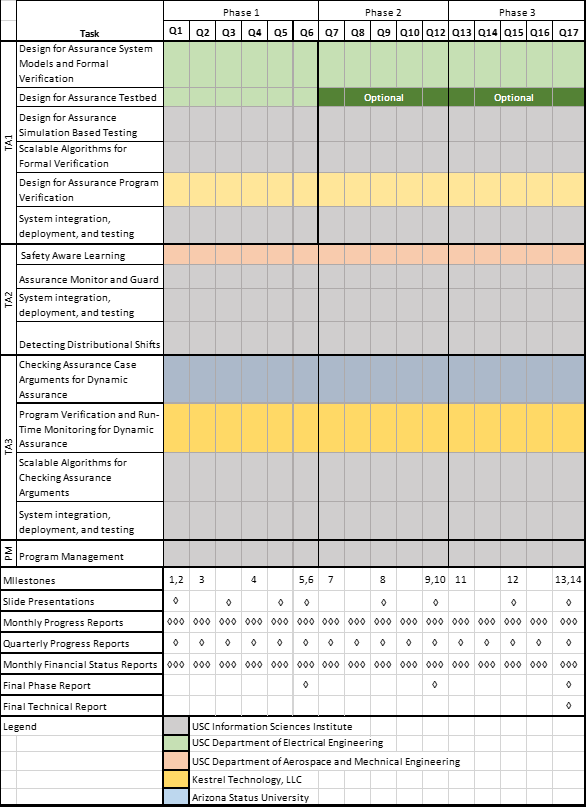
\includegraphics[width=.95\textwidth]{figs/Safeguard_Schedule_V6}
\end{center}
\vspace{-.2in}\caption{Project schedule along with a summary of milestones.  The legend maps task color to organization primary responsible for the task. } 
\label{fig:sandm}
\end{figure}
 

% \section{Level of Effort by Task \textcolor{red}{[Mike/Lisa - 1 pages]}}

% \textcolor{blue}{
% \begin{itemize}
% \item Will be a separate spreadsheet
% \item
% \end{itemize}
% }

\section*{Appendix A: Team Members and Other Information}
\addcontentsline{toc}{section}{Appendix A: Team Members and Other Information}

\baades{This section is mandatory and must include all of the following
components. If a particular subsection is not applicable, state “NONE”.}

\vspace{1ex}

\noindent
\textbf{Team Member Identification}:

\vspace{1ex}

\baades{Provide a list of all team members including the
prime, subcontractor(s), and consultant(s), as applicable. Identify specifically
whether any are a non-US organization or individual, FFRDC and/or Government
entity.}

\begin{centering}

%\small
\begin{tabular}{|p{1.8in}|p{1in}|p{1.1in}|p{0.7in}|p{0.8in}|p{0.7in}|}
\hline
 \textbf{Name} &  \textbf{Role} & \textbf{Organization} & \textbf{Non-US Org?}  & \textbf{Non-US Ind?} &  \textbf{FFRDC or Gov} \\
 \hline
Craig A. Knoblock & Prime & USC & N & N & N\\ \hline
Michael Orosz & Prime & USC & N &  N & N \\ \hline
Satish Thittamaranahalli & Prime & USC & N &  Y & N \\ \hline
Ryan Goodfellow & Prime & USC & N &  N & N \\ \hline
Anoop Kumar & Prime & USC & N & N & N \\ \hline
Satyandra Gupta & Prime & USC & N & N & N \\ \hline
Pierluigi Nuzzo & Prime & USC & N & Y & N \\ \hline
Petros Ioannou & Prime & USC & N & N & N \\ \hline
Chitta Baral & Subcontractor & ASU & N & N & N \\ \hline
Matt Barry & Subcontractor & Kestrel Technology & N & N & N \\ \hline
Douglas Smith & Subcontractor & Kestrel Technology & N & N & N \\ \hline
Henny Sipma & Subcontractor & Kestrel Technology & N & Y & N \\ \hline
\end{tabular} 
\end{centering}

\vspace{1ex}

\noindent
\textbf{Government or FFRDC Team Member Proof of Eligibility to Propose}: NONE

\baades {If
none of the team member organizations (prime or subcontractor) are a
Government entity or FFRDC, state “NONE”.}

\vspace{1ex}

\noindent
\textbf{Government or FFRDC Team Member Statement of Unique Capability}: NONE

\vspace{1ex}

\noindent
\textbf{Organizational Conflict of Interest Affirmations and Disclosure}: NONE

\vspace{1ex}

\noindent
\textbf{Intellectual Property (IP)}: 
\baades {
If no IP restrictions are intended, state “NONE”.
The Government will assume unlimited rights to all IP not explicitly identified as
having less than unlimited rights in the proposal.
For all technical data or computer software that will be furnished to the
Government with other than unlimited rights, provide (per Section VI.B.1) a list
describing all proprietary claims to results, prototypes, deliverables or systems
supporting and/or necessary for the use of the research, results, prototypes
and/or deliverables. Provide documentation proving ownership or possession of
appropriate licensing rights to all patented inventions (or inventions for which a
patent application has been filed) to be used for the proposed project.
}
\begin{centering}

%\small
\begin{tabular}{|p{2.1in}|p{1.2in}|p{1.4in}|p{2in}|}
\hline
\multicolumn{4}{|c|}{COMMERCIAL ITEMS }\\ \hline 
 \textbf{Technical Data, Computer Software To be Furnished With Restrictions} &  \textbf{Basis for Assertion} & \textbf{Asserted Rights Category} & \textbf{Name of Person Asserting Restrictions}  \\  \hline
KT Advance & Developed with mixed funding. & Restricted & David Kulich, Contracts Manager, Kestrel technology, LLC.\\ \hline
\end{tabular} 
\end{centering}

\vspace{1ex}

\noindent
\textbf{Human Subjects Research (HSR)}: NONE

\vspace{1ex}

\noindent
\textbf{Animal Use}: NONE

\vspace{1ex}

\noindent
\textbf{Representations Regarding Unpaid Delinquent Tax Liability or a Felony
Conviction under Any Federal Law}: 
%NONE

\begin{enumerate}
\item
The proposer is  not a corporation that has any unpaid Federal tax liability that has been assessed, for which all judicial and administrative remedies have been exhausted or have lapsed, and that is not being paid in a timely manner pursuant to an agreement with the authority responsible for collecting the tax liability,
\item
The proposer is not a corporation that was convicted of a felony criminal violation under a Federal law within the preceding 24 months.
\end{enumerate}

\vspace{1ex}

\noindent
\textbf{Cost Accounting Standards (CAS) Notices and Certification}:
\baades{
For any proposer who submits a proposal which, if accepted, will result in a CAS-compliant
contract, must include a Disclosure Statement as required by 48 CFR
9903.202. The disclosure forms may be found at
http://www.whitehouse.gov/omb/procurement\_casb
If this section is not applicable, state “NONE”. For further information regarding
this subject, please see www.darpa.mil/work-with-us/additional-baa.
}
NONE


%\section{Appendix B \textcolor{red}{[No Page Count]}}

\section{References}
\bibliographystyle{acm} 
\bibliography{TA3/ta3,TA2/ta2,TA1/ta1}
\end{document}
%%\documentclass[a4paper]{article}
%\documentclass[12pt]{article}
\documentclass[12pt]{dod-blank}

%% Language and font encodings
\usepackage[english]{babel}
\usepackage[utf8x]{inputenc}
\usepackage[T1]{fontenc}

%% Sets page size and margins
%%\usepackage[a4paper,top=3cm,bottom=2cm,left=3cm,right=3cm,marginparwidth=1.75cm]{geometry}
%\usepackage[top=1in, bottom=1in, left=1in, right=1in]{geometry}



%% Useful packages
\usepackage{amsmath}
\usepackage{graphicx}
  \graphicspath{{.}{./image/}}
  \DeclareGraphicsExtensions{.png,.jpg} 
\usepackage[colorinlistoftodos]{todonotes}
\usepackage[colorlinks=true, allcolors=blue]{hyperref}
\usepackage{tabularx}
\usepackage{multirow}
\usepackage{tabulary}
\usepackage{float}
\usepackage{wrapfig}
\usepackage[export]{adjustbox}
\usepackage{comment}
\usepackage{tabularx}
\usepackage{multirow}
\usepackage{tabulary}
\usepackage{enumitem}

\usepackage{listings}
\usepackage{color}
\usepackage{array}
\usepackage{subcaption}
\usepackage{xcolor}




\renewcommand{\textfraction}{0}
\renewcommand{\topfraction}{1.0}
\renewcommand{\bottomfraction}{1.0}

\usepackage{longtable}
%% macros
\newif\iffinal
\finaltrue
\iffinal
  
    \newcommand\baareq[1]{}
    \newcommand\baades[1]{}
 
 
\else
    \definecolor{darkgreen}{rgb}{0,0.4,0}
    \definecolor{darkcyan}{rgb}{0,0.4,0.4}
    \definecolor{darkblue}{rgb}{0,0,0.5}
    
    \newcommand\baareq[1]{{\color{darkcyan}[\textbf{Requirement:} #1]}}
    \newcommand\baades[1]{{\color{darkcyan}[\textbf{Description:} #1]}}
 
\fi




\def\naive{na\"{\i}ve}



\lstset{ 
  backgroundcolor=\color{white},   % choose the background color; you must add \usepackage{color} or \usepackage{xcolor}
  basicstyle=\footnotesize\ttfamily,            % the size of the fonts that are used for the code
  breakatwhitespace=false,         % sets if automatic breaks should only happen at whitespace
  breaklines=true,                 % sets automatic line breaking
  captionpos=b,                    % sets the caption-position to bottom
  commentstyle=\color{mygreen},    % comment style
  % deletekeywords={...},            % if you want to delete keywords from the given language
  escapeinside={\%*}{*)},          % if you want to add LaTeX within your code
  extendedchars=true,              % lets you use non-ASCII characters; for 8-bits encodings only, does not work with UTF-8
  frame=single,	                   % adds a frame around the code
  keepspaces=false,                 % keeps spaces in text, useful for keeping indentation of code (possibly needs columns=flexible)
  keywordstyle=\color{blue}\bfseries\underbar,       % keyword style
  language=Prolog,                 % the language of the code
  % morekeywords={if,and},        % if you want to add more keywords to the set
  numbers=none,                    % where to put the line-numbers; possible values are (none, left, right)
  numbersep=5pt,                   % how far the line-numbers are from the code
  numberstyle=\tiny\color{mygray}, % the style that is used for the line-numbers
  rulecolor=\color{black},         % if not set, the frame-color may be changed on line-breaks within not-black text
  showspaces=false,                % show spaces everywhere adding particular underscores; it overrides 'showstringspaces'
  showstringspaces=false,          % underline spaces within strings only
  showtabs=false,                  % show tabs within strings adding particular underscores
  stepnumber=2,                    % the step between two line-numbers. If it's 1, each line will be numbered
  stringstyle=\color{mymauve},     % string literal style
  tabsize=2,	                   % sets default tabsize to 2 spaces
  title=\lstname                   % show the filename of files included with \lstinputlisting; also try caption instead of title
}

% apply trick for additional keywords for our AC DSL
\lstset{
	emph={for, if, and, or},
    emphstyle={\color{blue}\bfseries\underbar}
}




\title{DARPA Assured Autonomy}
\author{Technical Volume- \textcolor{red}{Thirty-Eight (38) pages max}}

\begin{document}
\pagenumbering{roman}
 
\begin{center}
\large{\textbf{Volume 1: Technical and Management Proposal}}
\end{center}
\textbf{BAA Number:} DARPA-HR001117S0045 \\
\textbf{Technical Area:} TA1, TA2, and TA3 \\
\textbf{Proposal Title:} Assured Autonomy for Learning Enabled Vehicles (Safeguard) \\
\textbf{Lead Institution:} University of Southern California \\
\textbf{Type of organization: } “OTHER EDUCATIONAL” \\

\begin{tabularx}{\linewidth}{XX}

 \textbf{Technical Point of Contact} &  \textbf{Administrative Point of Contact }   \\
Dr.\ Craig A. Knoblock  & Sapphire Masterson  \\ 
USC Information Sciences Institute & USC Dept. of Contracts \& Grants \\
4676 Admiralty Way, Suite 1001 & 4676 Admiralty Way, Suite 1001 \\
Marina del Rey, CA 90292 & Marina del Rey, CA 90292 \\
Tel: 310-448-8786 &  Tel: (310) 448-9161 \\
E-mail: knoblock@isi.edu  & E-mail: sapphirm@usc.edu \\
\end{tabularx}
\\
\\
\textbf{Award instrument requested:}  Procurement Contract, Cost-Reimbursement, No Fee
\\
\\
\textbf{Total amount of the proposed effort:} \$ ...\\
Phase I: \$ ... \\
Phase II: \$ ... \\
Phase III: \$ ... \\
\\
\textbf{Place(s) of performance:} USC, Marina del Rey, CA; Los Angeles, CA;  Tempe, AZ; Palo Alto, CA \\
\textbf{Period(s) of performance:} 04/02/2018 - 03/31/2022     \\
\\
\textbf{Other team members:} \\
\begin{tabularx}{\linewidth}{XX}
Kestrel Technology  & Arizona State University \\
(small business) & (Other Educational)\\
POC: Matthew Barry & POC: Chitta Baral\\
3260 Hillview Avenue & Department of Computer Science and Engr. \\
Palo Alto, CA 94304 & Ira A. Fulton School of Engineering \\ 
phone: (832)205-4876 & Arizona State University\\ 
mrbarry@kestreltechnology.com & Brickyard Suite 572, 699 S. Mill Avenue \\
& Tempe, AZ 85281-8809, U.S.A.\\
& email: chitta@asu.edu\\
\end{tabularx}
\\
\textbf{Proposal validity period: } 180 days\\
\\
\textbf{Data Universal Numbering System (DUNS) number: } 072933393\\
\textbf{Taxpayer identification number:} 95-1642394\\
\textbf{Commercial and Government Entity (CAGE) code:} 1B729 Marina del Rey, CA\\
\textbf{Proposer’s reference number (if any):}  4409-0\\

\newpage
\section{Table of Contents}
\tableofcontents

\newpage
\pagenumbering{arabic}
\section{Executive Summary}
As we rapidly move into a world where machine learning plays a central role in realizing autonomous systems, it is becoming increasingly important to develop techniques that assure that these systems will operate safely and perform as expected. Current approaches are limited to providing assurance for systems with limited or no  learning capabilities. In this context, DARPA's Assured Autonomy BAA seeks to \emph{develop rigorous design and analysis technologies for continual assurance of learning-enabled autonomous systems}. USC in collaboration with Kestrel Technology and ASU is pleased to submit a comprehensive TA1, TA2, and TA3 proposal entitled \emph{``Assured Autonomy for Learning Enabled Vehicles (Safeguard).''} We plan to provide an end-to-end solution to support autonomous systems with learning-enabled components, ranging from design technologies for assurance, to assurance monitoring and control techniques, to representation and online evaluation of assurance cases. We have assembled a strong team of experts that cover the range of technologies that are required to create such an end-to-end system. If successful, the project will provide the technologies for building the next-generation of learning-enabled autonomous systems.  The entire project will take four years and cost \textcolor{red}{\$??}, with an initial version completed at the end of Phase I and successive versions with additional capabilities and improved scalability at the end of Phase II and Phase III.  

In the remainder of this section, we first introduce an  unmanned surface vehicle scenario that will be used throughout the proposal to describe the approach.  Next, we describe our approach to design, monitoring, and dynamic assurance. Finally, we introduce the team involved in the project. 

\textbf{Motivating Scenario.} Consider an autonomous unmanned surface vehicle (USV) guarding a valuable asset in the ocean when an unknown vehicle  approaches the security perimeter, under challenging weather conditions. In this scenario, the USV is required to approach the intruding vehicle, issue a warning signal, and escort it to a safe distance from the controlled area. However, as the USV has no a priori knowledge of its external environment behaviors (e.g., water depth, waves, wind, current, visibility), pre-computing a feasible trajectory, let alone optimal, becomes a non-trivial problem. For trajectory planning, the USV must continuously perform the following tasks:
\begin{itemize}[itemsep=0pt,leftmargin=*]
 \item Sense the current state of the surrounding environment (e.g., water depth, waves, wind, current, visibility) and estimate its own maneuverability constraints (e.g., braking distance, available acceleration, maximum velocity, turning radius, turning rate, safety distance) based on the state of the environment;      
\item Sense the static obstacles in the sensor range and generate a traversability map;
\item Sense the moving obstacles and classify them;   
\item Predict future trajectories of moving obstacles; 
\item Determine if any of the COLREGS \cite{commandant1999international} rules will be in effect with respect to one or more of the nearby vessels and identify the vessels with the right of way.    
\end{itemize}
The above information will be used by the trajectory planner to compute an initial trajectory, which will be continuously refined as the USV gathers additional information.
% It is not possible for the USV to be tested in every possible environment. 
The USV will use learning enabled components to take  decisions as it encounters new situations, such as  
\begin{itemize}[itemsep=0pt,leftmargin=*]
\item Classifiers to identify moving obstacles based on physical appearance and motion signatures,
\item Algorithms to estimate the sensor capabilities in adverse weather conditions,   
\item Algorithms to accurately estimate uncertainty in the environment, 
\item Classifiers to generate traversability maps,
\item Prediction of external vessel behaviors based on motion histories, 
\item Reinforcement learning  to ensure COLREGS compliance of maneuvers,  
\item Algorithms to learning pursuit behaviors.  
\end{itemize}
Learning enabled components will interact with each other in complex ways, where a misclassification error in one component may eventually compromise the entire mission.   
% We will need to make sure that each learning enabled components has a run-time monitor that will ensure that the assumptions made by the learning-enabled component remain valid and prevent erroneous learning. 
% For example, if the vehicle is exhibiting significant error in trajectory tracking, then simply downgrading the trajectory tracking error value may not be a good option.  The failure of prediction of trajectory tracking error might be due to the presence of a significant wake caused by a nearby vessel. The presence of the nearby vessel can be used to explain the degradation in trajectory tracking performance. As the vessel moves away, we can expect the trajectory tracking performance to return to the predicted level.  
While exhaustive validation of learning-enabled cyber-physical systems (LE-CPSs) is a prohibitive task~\cite{Kalra16},
their complexity, heterogeneity, and highly dynamic nature
make it challenging to even leverage existing model-based development techniques to effectively assess system correctness 
% dependability, 
at design time or enforce it at runtime.

\textbf{Design for Assurance.} Safeguard uses a platform-based design approach~\cite{Nuzzo15b} to organize the design process for a LE-CPS and to build assurance cases. Composite models are developed at several levels of abstraction,
from top-level system requirements and safety constraints down to the
implementation level.  Intermediate levels add detail to the levels
above.  The different levels are connected by refinement mappings that
allow properties established at one level to be preserved at the next
level (see Figures~\ref{fig:methodology} and~\ref{fig:assurance}).

Contracts are used to formally specify components and composite models
in terms of (1) Assumptions -- the assumed behaviors of the
environment and the behaviors of other components, and (2) Guarantees
-- the behavior properties that a model guarantees if it operates in a
context that satisfies its assumptions.  A calculus of contracts
allows horizontal composition of contracts to generate contracts for
composite models.  Vertical contracts are used to specify the mapping
or refinement relation between models at different levels of
abstraction.  The system design process starts with a high-level
contract that expresses overall system assumptions and requirements.
Subsequent levels express models with increasing detail until the
lowest level expresses the system in terms of hardware components and
their software controllers.

The assurance case for a CPS arises from the horizontal and vertical
structure of the design in several ways.  The components used within a
particular level are either (1) synthesized using
correct-by-construction design tools together with proofs, (2) derived
statically or dynamically using safety-aware machine-learning
techniques, (3) written manually and verified by analysis tools, or
(4) written manually and validated by extensive testing.  The
assurance case for the whole reflects its compositional structure.  We
anticipate that well-specified contracts together with the calculus of
contracts will eliminate well-known problems with unexpected emergent
behaviors in CPS systems.

The assurance case for the lowest-layer design arises from both the
intra-level assurance and from properties and their proofs that are
preserved under the refinement mapping from the top-level
requirements.  The refinement mappings between model layers will be
constructed using a variety of techniques.  A contract at an abstract
level can be mapped to a component or refined contract by (1)
retrieval of pre-verified components from a platform library, (2)
synthesis using correct-by-construction design and optimization tools,
or (3) manual coding to satisfy a contract.  The mapping of a
composite model will be composed from the mappings of its constituent
components or contracts.  When a composite model cannot be mapped
compositionally to the next level, it will be generated using
correct-by-construction design and optimization tools.

\textbf{Assurance Monitoring and Control.}
We provide an integrated framework for safety-aware learning, assurance monitoring and control, detecting distribution shifts. Three major components offer an efficient TA2 architecture as well as interfaces with TA1 and TA3, that is, (a) safety-aware learning and planning, (b) assurance monitors for guarding architectural and safety constraints; and (c) distribution shift detection.

We will develop a new learning-enabled online decision-making framework that allows opportunistically composing a sequence of actions (maneuvers) to reduce uncertainty in the system capability model without suspending the progress toward the mission goals or compromising safety. Each candidate action is evaluated based on three criteria: (1) the risk of violating a safety constraint using the current uncertainties in the parameter estimates; (2) its relevance to the mission goals; (3)  its expected information gain, i.e., reduction in uncertainty, with respect to the parameter estimates. These evaluations are combined to produce a cumulative mission utility value for each action that drives our learning-enabled decision-making framework. The problem of generating and evaluating sequences of actions can be posed in several way. For example, it can be solved using a branch-and-bound search method like Anytime A*, or formulated with the finite-horizon Markov Decision Process (MDP) framework. We will develop new scalable search strategies to solve this problem efficiently, by potentially evaluating a recent method developed at USC, called FastMap, that can significantly improve the execution time. 

We will develop monitors for architectural and safety constraints. 
% While these constraints can be checked over and over again as sensor information flow in, this naive strategy accounts for a lot of computational overhead. 
To achieve scalability and decrease the overhead, we propose the application of a technique that we currently use in DARPA's RSPACE program, which leverages a physical model of the vehicles dynamics and its interactions with the environment to efficiently determine the readout frequency. We propose two  extensions of this basic idea. First, we will use the theory of Variable Elimination to prioritize which variables to monitor, e.g., controllable, versus uncontrollable, adversarially controlled, or unobservable variables. Second, we invoke the dynamic assessment of assurance cases only when needed. This  decreases the number of times dynamic assessment of assurance cases is initiated as well as the communication bandwidth between the TA2 and TA3 components.

Finally, we will identify a distribution shift by combining statistical and machine learning techniques to differentiate between environmental and sensor changes. We will exploit a categorization of the shifts based on their cause and duration as well as extend our earlier work on detecting and mitigating sensor failures for all types of monitored variables.  

\textbf{Dynamic Assurance:} The Safeguard {\em design for assurance\/} activity takes a systems-theoretic stance toward safety.  Consequently, it presumes that safety is an emergent property of the system, and that hazards can present themselves through unintended interactions and performance violations in addition to causal events such as component failures.  Our design approach includes consideration of intent as well as hazard analysis and mitigation.  The artifacts from these activities populate contracts and assumptions for the dynamic assurance case.  
We thus build safety into the product by working at a systems-level viewpoint, using lexicon and design patterns familiar to both hardware and software engineers; safety is an emergent property of the system, not an afterthought.  
As system behavior evolves during runtime owing to learning, threats, degradation, or some other factor, the dynamic assurance case identifies whether the safety constraints continue to be satisfied.  If not, it provides notifications or issues recovery instructions directly from a lookup table.

Our implementation of the dynamic assurance case employs a declarative knowledge base inference engine and a domain-specific language tailored to our approach.  We have used them successfully for assurance case tool sets and arguments, and will extend them to reason about uncertainty and learning.  Our approach to achieve scalability is to specialize solvers toward modularity and to take advantage of domain knowledge.  Specifically, we will develop answer set programming techniques for context-dependent learning for reasoning about the learning-enabled components as well as learning assurance rules.  We will develop new formalisms for uncertainty to include causality, using weights for computing probabilities, and probabilistic non-monotonicity.  To achieve scaling objectives we will implement specializations using modularity, weighted CSPs, and message passing. 

% The system safety constraints revealed from that design become the key elements of our dynamic assurance case.  Our verification tools ensure the constraints are relevant, identifiable, and their implementation and effect observable.  

\textbf{Team.} We have assembled a team that is exceptionally well-qualified to build the proposed Safeguard system.  The team will be led by Dr.\ Craig Knoblock, the Principal Investigator for the effort, who currently leads the Intelligent Systems Division at the Information Sciences Institute.  He has led many large DARPA and IARPA projects over the years and has a strong track record in conducting leading edge research and then transitioning the technology to commercial use.  He will be supported by Dr.\ Michael Orosz as the Project Manager, who also has  experience in managing large research projects and on autonomous systems.  The TA1 team will be led by Dr.\ Pierluigi Nuzzo, who is an expert in embedded system design methodologies and the  application of formal methods to cyber-physical systems.  The TA1 team also includes Dr.\ Doug Smith, who has spent many years working on scalable correct-by-construction techniques and Dr.\ Henny Sipma, who has significant experience in applying program verification methods to real-world problems.  The TA1 team also includes Ryan Goodfellow, who has done a large amount of work on simulation-based testing.  The TA2 team will be led by Dr.\ Knoblock who has worked on topics related to both monitoring and detecting distribution changes.  He will be supported by Dr.\ Satyandra Gupta, who is an expert on autonomous surface vehicles as well as on safety-aware learning. He will also be supported by Drs.\ Anoop Kumar and Satish Thittamaranahalli, who have also previously worked on efficient methods for execution monitoring.  The TA3 team will be lead by Dr.\ Matthew Barry, who has experience in creating the technologies for assurance cases.  He will be supported by Dr.\ Chitta Baral, who is an expert on ASP solvers and by Dr.\ Thittamaranahalli who is an expert on SAT solvers, both of which will be applied to provide scalable assurance case reasoning.  Finally, Dr.\ Petros Ioannou, who is an expert on control systems for autonomous vehicles will provide an autonomous vehicle platform, which will form the focus of our work until the TA4 teams provide additional vehicle platforms for development.  

\newpage
\section{Innovative Claims and Deliverables}

In this project we will develop and build an end-to-end system for assured autonomy.  This section describes the key innovations by technical area and then the overall deliverables of the project.

\paragraph{Design for Assurance}

\begin{itemize}[itemsep=0pt,leftmargin=*]
\item We address the LE-CPS design challenges via a holistic approach that can contextually generate design artifacts and assurance cases. We develop a compositional, contract-based modeling framework, methods, and tools to support the design process from system-level requirement capture,  formalization, and analysis, to the generation, testing, and continual monitoring of software and hardware artifacts in feedback loop with a physical process.

\item We develop compositional abstractions and interfaces (vertical contracts) that can  bridge heterogeneous formalisms and heterogeneous decomposition architectures to make system analysis and synthesis tractable, consistently combine different verification and synthesis methods at design time, and provide seamless support for dynamic assurance at run time. %We aim to quantitatively capture the confidence in the satisfaction of requirements under uncertain or unknown conditions, and resilience properties of  systems at different abstraction levels, to enable trade-off evaluation between resilience, performance, and cost.

\item We develop a unifying framework and efficient algorithms to reason about the combination of discrete and continuous dynamics and constraints in the presence of uncertainties in LE-CPS using a satisfiability modulo convex approach~\cite{Shoukry2017} for contract-based system verification and scalable trajectory planning.  

\item We provide an environment for high-fidelity CPS testing, in which production-ready software, e.g.,  safety-critical learning and control, may be deployed and tested 
% by extending the Cypress testbed environment \cite{Goodfellow2015Cypress:Systems} 
with time dilation facilities, so that it synchronizes with a physical simulation that is not necessarily running in real time, while still having the perception of real time.

\item We 
% These facilities allow a cyber system to be  
propose an approach for unanticipated behavior space identification and test coverage maximization which leverages results from the theory of differential algebraic equation (DAE)~\cite{Berger2013ControllabilitySurvey,Ilchmann2005ATheory,BergerOnSystems,Lamour2013} 
to prune the behavior search space and identify smaller regions of interest for efficient simulation-based testing. 
% We then compute the intersection of these two behavior spaces and restrict our simulation based testing search space to this subspace.
\end{itemize}

\paragraph{Assurance Monitoring and Control}

\begin{itemize}[itemsep=0pt,leftmargin=*]
\item 
%We integrate safety-aware learning into the overall decision making problem. The goal is to maximize mission utility without violating the safety constraints. 
Our safety-aware learning framework enables the system to opportunistically select and execute actions to assist the learning-enabled component in reducing model uncertainty without compromising safety or deviating from the mission goals. The value of uncertainty reduction is explicitly incorporated in the optimization process for selecting the best action.  
\item For safety-aware learning, we propose the idea of preprocessing the search space of the problem domain before queries and observations come in. With such a linear-time preprocessing phase, the performance of search and optimization algorithms can be significantly boosted. For example, in regular A* search, the intensional or extensional search space can be preprocessed in near-linear time to yield an embedding of each state as a point in Euclidean space~\cite{cujakk}. Then, when the query comes in, A* search can make use of these Euclidean distances as heuristic distances between two states to yield order-of-magnitude speedups. 
%In Anytime A* for safety-aware learning and planning, this leads to a significantly better quality of actions chosen within a time limit, and in the MDP framework, the same ideas can be used to improve the convergence of Bellman updates for safety-aware Reinforcement Learning.
\item As massive amounts of sensor information flow in, it is imperative for us to efficiently process this information for monitoring architectural and safety constraints. Building on our past work on similar tasks, we propose novel technologies for efficiently monitoring constraints. These algorithms can yield an exponential reduction in the amount of sensor data that needs to be processed. Doing this also reduces the message complexities between the various modules. %We also propose to use the theory of Variable Elimination (VE) to monitor constraints with uncontrollable, adversarially controlled, and/or unobservable variables. VE yields a substrate constraint to monitor that characterizes a dominant strategy of the controllable variables over the uncontrollable, adversarially controlled, and/or unobservable variables.
\item We will develop techniques to identify  distributional shifts and determine the underlying cause (e.g., change in environment, sensor failure,   etc.), as well as strategies for handling the various distributional shifts.   Notably, we propose to build on our past work and use compact representations to exploit historical data to identify distributional shifts.
\end{itemize}

\paragraph{Dynamic Assurance}

\begin{itemize}[itemsep=0pt,leftmargin=*]

\item We demonstrate the integration of dynamic assurance for safety-critical learning-enabled dynamic systems in which evolutionary behaviors are expected and tolerated as a property of the functionality.   The impact will be consequential contributions safety-critical dynamic systems in which evolutionary behaviors are expected and tolerated as portion of the functionality.   
\item We implement dynamic assurance by combining features of system safety, formal methods, logic programming, uncertain reasoning, and domain-specific languages.  We populate assurance case arguments at several levels of modeling and implementation abstraction, using the analysis results to produce design-time evidence supporting assurance claims.  
%We provide automated reasoning about the assurance case itself to produce verification, consistency, and completeness results for the argument.  Dynamic assurance results then yield trusted explanations of whether safety constraints and assumptions and other contracts still hold during the collection of runtime evidence from monitors. 
\item We develop and demonstrate ASP formalisms crucial to applications in dynamic assurance. We demonstrate the suitability of the technology especially for assurance case arguments owing to the improved legibility, consistency and completeness checks, handling of uncertain and default reasoning, and scalability.  
%We will produce modularized solvers for enhanced performance based on recent algorithmic developments in exploiting structure, kernelization, and message passing. We provide a formalism to enable learning of assurance rules. 
We provide a novel approach to handling uncertainty that provides the ability to do causal and counter-factual reasoning as well as probabilistic non-monotonicity.  Overcoming limitations of traditional inductive logic techniques, we develop a novel iterative and incremental approach based on context dependent learning. 
\end{itemize}

\paragraph{Deliverables}
During the course of this project, we will build and deliver a fully-operational system that covers all three of the technical areas.  The detailed capabilities of this system are described in the individual technical sections.  The resulting system will be available as open source under a permissive license, which will allow other organizations to use the work, extend it in new directions, and even commercialize the software.  Kestrel Technology has significant experience in this space and has built and applied these types of technologies to a variety of real world tasks.  Kestrel is ideally suited to pursue commercial uses of this technology and the permissive license will facilitate exploring these opportunities since there will be no need to negotiate intellectual property rights.  

\newpage
\section{Technical Plan}
%%\documentclass[a4paper]{article}
%\documentclass[12pt]{article}
\documentclass[12pt]{dod-blank}

%% Language and font encodings
\usepackage[english]{babel}
\usepackage[utf8x]{inputenc}
\usepackage[T1]{fontenc}

%% Sets page size and margins
%%\usepackage[a4paper,top=3cm,bottom=2cm,left=3cm,right=3cm,marginparwidth=1.75cm]{geometry}
%\usepackage[top=1in, bottom=1in, left=1in, right=1in]{geometry}



%% Useful packages
\usepackage{amsmath}
\usepackage{graphicx}
  \graphicspath{{.}{./image/}}
  \DeclareGraphicsExtensions{.png,.jpg} 
\usepackage[colorinlistoftodos]{todonotes}
\usepackage[colorlinks=true, allcolors=blue]{hyperref}
\usepackage{tabularx}
\usepackage{multirow}
\usepackage{tabulary}
\usepackage{float}
\usepackage{wrapfig}
\usepackage[export]{adjustbox}
\usepackage{comment}
\usepackage{tabularx}
\usepackage{multirow}
\usepackage{tabulary}
\usepackage{enumitem}

\usepackage{listings}
\usepackage{color}
\usepackage{array}
\usepackage{subcaption}
\usepackage{xcolor}




\renewcommand{\textfraction}{0}
\renewcommand{\topfraction}{1.0}
\renewcommand{\bottomfraction}{1.0}

\usepackage{longtable}
%% macros
\newif\iffinal
\finaltrue
\iffinal
  
    \newcommand\baareq[1]{}
    \newcommand\baades[1]{}
 
 
\else
    \definecolor{darkgreen}{rgb}{0,0.4,0}
    \definecolor{darkcyan}{rgb}{0,0.4,0.4}
    \definecolor{darkblue}{rgb}{0,0,0.5}
    
    \newcommand\baareq[1]{{\color{darkcyan}[\textbf{Requirement:} #1]}}
    \newcommand\baades[1]{{\color{darkcyan}[\textbf{Description:} #1]}}
 
\fi




\def\naive{na\"{\i}ve}



\lstset{ 
  backgroundcolor=\color{white},   % choose the background color; you must add \usepackage{color} or \usepackage{xcolor}
  basicstyle=\footnotesize\ttfamily,            % the size of the fonts that are used for the code
  breakatwhitespace=false,         % sets if automatic breaks should only happen at whitespace
  breaklines=true,                 % sets automatic line breaking
  captionpos=b,                    % sets the caption-position to bottom
  commentstyle=\color{mygreen},    % comment style
  % deletekeywords={...},            % if you want to delete keywords from the given language
  escapeinside={\%*}{*)},          % if you want to add LaTeX within your code
  extendedchars=true,              % lets you use non-ASCII characters; for 8-bits encodings only, does not work with UTF-8
  frame=single,	                   % adds a frame around the code
  keepspaces=false,                 % keeps spaces in text, useful for keeping indentation of code (possibly needs columns=flexible)
  keywordstyle=\color{blue}\bfseries\underbar,       % keyword style
  language=Prolog,                 % the language of the code
  % morekeywords={if,and},        % if you want to add more keywords to the set
  numbers=none,                    % where to put the line-numbers; possible values are (none, left, right)
  numbersep=5pt,                   % how far the line-numbers are from the code
  numberstyle=\tiny\color{mygray}, % the style that is used for the line-numbers
  rulecolor=\color{black},         % if not set, the frame-color may be changed on line-breaks within not-black text
  showspaces=false,                % show spaces everywhere adding particular underscores; it overrides 'showstringspaces'
  showstringspaces=false,          % underline spaces within strings only
  showtabs=false,                  % show tabs within strings adding particular underscores
  stepnumber=2,                    % the step between two line-numbers. If it's 1, each line will be numbered
  stringstyle=\color{mymauve},     % string literal style
  tabsize=2,	                   % sets default tabsize to 2 spaces
  title=\lstname                   % show the filename of files included with \lstinputlisting; also try caption instead of title
}

% apply trick for additional keywords for our AC DSL
\lstset{
	emph={for, if, and, or},
    emphstyle={\color{blue}\bfseries\underbar}
}




\title{DARPA Assured Autonomy}
\author{Technical Volume- \textcolor{red}{Thirty-Eight (38) pages max}}

\begin{document}
\pagenumbering{roman}
\include{cover}

\newpage
\section{Table of Contents}
\tableofcontents

\newpage
\pagenumbering{arabic}
\section{Executive Summary}
As we rapidly move into a world where machine learning plays a central role in realizing autonomous systems, it is becoming increasingly important to develop techniques that assure that these systems will operate safely and perform as expected. Current approaches are limited to providing assurance for systems with limited or no  learning capabilities. In this context, DARPA's Assured Autonomy BAA seeks to \emph{develop rigorous design and analysis technologies for continual assurance of learning-enabled autonomous systems}. USC in collaboration with Kestrel Technology and ASU is pleased to submit a comprehensive TA1, TA2, and TA3 proposal entitled \emph{``Assured Autonomy for Learning Enabled Vehicles (Safeguard).''} We plan to provide an end-to-end solution to support autonomous systems with learning-enabled components, ranging from design technologies for assurance, to assurance monitoring and control techniques, to representation and online evaluation of assurance cases. We have assembled a strong team of experts that cover the range of technologies that are required to create such an end-to-end system. If successful, the project will provide the technologies for building the next-generation of learning-enabled autonomous systems.  The entire project will take four years and cost \textcolor{red}{\$??}, with an initial version completed at the end of Phase I and successive versions with additional capabilities and improved scalability at the end of Phase II and Phase III.  

In the remainder of this section, we first introduce an  unmanned surface vehicle scenario that will be used throughout the proposal to describe the approach.  Next, we describe our approach to design, monitoring, and dynamic assurance. Finally, we introduce the team involved in the project. 

\textbf{Motivating Scenario.} Consider an autonomous unmanned surface vehicle (USV) guarding a valuable asset in the ocean when an unknown vehicle  approaches the security perimeter, under challenging weather conditions. In this scenario, the USV is required to approach the intruding vehicle, issue a warning signal, and escort it to a safe distance from the controlled area. However, as the USV has no a priori knowledge of its external environment behaviors (e.g., water depth, waves, wind, current, visibility), pre-computing a feasible trajectory, let alone optimal, becomes a non-trivial problem. For trajectory planning, the USV must continuously perform the following tasks:
\begin{itemize}[itemsep=0pt,leftmargin=*]
 \item Sense the current state of the surrounding environment (e.g., water depth, waves, wind, current, visibility) and estimate its own maneuverability constraints (e.g., braking distance, available acceleration, maximum velocity, turning radius, turning rate, safety distance) based on the state of the environment;      
\item Sense the static obstacles in the sensor range and generate a traversability map;
\item Sense the moving obstacles and classify them;   
\item Predict future trajectories of moving obstacles; 
\item Determine if any of the COLREGS \cite{commandant1999international} rules will be in effect with respect to one or more of the nearby vessels and identify the vessels with the right of way.    
\end{itemize}
The above information will be used by the trajectory planner to compute an initial trajectory, which will be continuously refined as the USV gathers additional information.
% It is not possible for the USV to be tested in every possible environment. 
The USV will use learning enabled components to take  decisions as it encounters new situations, such as  
\begin{itemize}[itemsep=0pt,leftmargin=*]
\item Classifiers to identify moving obstacles based on physical appearance and motion signatures,
\item Algorithms to estimate the sensor capabilities in adverse weather conditions,   
\item Algorithms to accurately estimate uncertainty in the environment, 
\item Classifiers to generate traversability maps,
\item Prediction of external vessel behaviors based on motion histories, 
\item Reinforcement learning  to ensure COLREGS compliance of maneuvers,  
\item Algorithms to learning pursuit behaviors.  
\end{itemize}
Learning enabled components will interact with each other in complex ways, where a misclassification error in one component may eventually compromise the entire mission.   
% We will need to make sure that each learning enabled components has a run-time monitor that will ensure that the assumptions made by the learning-enabled component remain valid and prevent erroneous learning. 
% For example, if the vehicle is exhibiting significant error in trajectory tracking, then simply downgrading the trajectory tracking error value may not be a good option.  The failure of prediction of trajectory tracking error might be due to the presence of a significant wake caused by a nearby vessel. The presence of the nearby vessel can be used to explain the degradation in trajectory tracking performance. As the vessel moves away, we can expect the trajectory tracking performance to return to the predicted level.  
While exhaustive validation of learning-enabled cyber-physical systems (LE-CPSs) is a prohibitive task~\cite{Kalra16},
their complexity, heterogeneity, and highly dynamic nature
make it challenging to even leverage existing model-based development techniques to effectively assess system correctness 
% dependability, 
at design time or enforce it at runtime.

\textbf{Design for Assurance.} Safeguard uses a platform-based design approach~\cite{Nuzzo15b} to organize the design process for a LE-CPS and to build assurance cases. Composite models are developed at several levels of abstraction,
from top-level system requirements and safety constraints down to the
implementation level.  Intermediate levels add detail to the levels
above.  The different levels are connected by refinement mappings that
allow properties established at one level to be preserved at the next
level (see Figures~\ref{fig:methodology} and~\ref{fig:assurance}).

Contracts are used to formally specify components and composite models
in terms of (1) Assumptions -- the assumed behaviors of the
environment and the behaviors of other components, and (2) Guarantees
-- the behavior properties that a model guarantees if it operates in a
context that satisfies its assumptions.  A calculus of contracts
allows horizontal composition of contracts to generate contracts for
composite models.  Vertical contracts are used to specify the mapping
or refinement relation between models at different levels of
abstraction.  The system design process starts with a high-level
contract that expresses overall system assumptions and requirements.
Subsequent levels express models with increasing detail until the
lowest level expresses the system in terms of hardware components and
their software controllers.

The assurance case for a CPS arises from the horizontal and vertical
structure of the design in several ways.  The components used within a
particular level are either (1) synthesized using
correct-by-construction design tools together with proofs, (2) derived
statically or dynamically using safety-aware machine-learning
techniques, (3) written manually and verified by analysis tools, or
(4) written manually and validated by extensive testing.  The
assurance case for the whole reflects its compositional structure.  We
anticipate that well-specified contracts together with the calculus of
contracts will eliminate well-known problems with unexpected emergent
behaviors in CPS systems.

The assurance case for the lowest-layer design arises from both the
intra-level assurance and from properties and their proofs that are
preserved under the refinement mapping from the top-level
requirements.  The refinement mappings between model layers will be
constructed using a variety of techniques.  A contract at an abstract
level can be mapped to a component or refined contract by (1)
retrieval of pre-verified components from a platform library, (2)
synthesis using correct-by-construction design and optimization tools,
or (3) manual coding to satisfy a contract.  The mapping of a
composite model will be composed from the mappings of its constituent
components or contracts.  When a composite model cannot be mapped
compositionally to the next level, it will be generated using
correct-by-construction design and optimization tools.

\textbf{Assurance Monitoring and Control.}
We provide an integrated framework for safety-aware learning, assurance monitoring and control, detecting distribution shifts. Three major components offer an efficient TA2 architecture as well as interfaces with TA1 and TA3, that is, (a) safety-aware learning and planning, (b) assurance monitors for guarding architectural and safety constraints; and (c) distribution shift detection.

We will develop a new learning-enabled online decision-making framework that allows opportunistically composing a sequence of actions (maneuvers) to reduce uncertainty in the system capability model without suspending the progress toward the mission goals or compromising safety. Each candidate action is evaluated based on three criteria: (1) the risk of violating a safety constraint using the current uncertainties in the parameter estimates; (2) its relevance to the mission goals; (3)  its expected information gain, i.e., reduction in uncertainty, with respect to the parameter estimates. These evaluations are combined to produce a cumulative mission utility value for each action that drives our learning-enabled decision-making framework. The problem of generating and evaluating sequences of actions can be posed in several way. For example, it can be solved using a branch-and-bound search method like Anytime A*, or formulated with the finite-horizon Markov Decision Process (MDP) framework. We will develop new scalable search strategies to solve this problem efficiently, by potentially evaluating a recent method developed at USC, called FastMap, that can significantly improve the execution time. 

We will develop monitors for architectural and safety constraints. 
% While these constraints can be checked over and over again as sensor information flow in, this naive strategy accounts for a lot of computational overhead. 
To achieve scalability and decrease the overhead, we propose the application of a technique that we currently use in DARPA's RSPACE program, which leverages a physical model of the vehicles dynamics and its interactions with the environment to efficiently determine the readout frequency. We propose two  extensions of this basic idea. First, we will use the theory of Variable Elimination to prioritize which variables to monitor, e.g., controllable, versus uncontrollable, adversarially controlled, or unobservable variables. Second, we invoke the dynamic assessment of assurance cases only when needed. This  decreases the number of times dynamic assessment of assurance cases is initiated as well as the communication bandwidth between the TA2 and TA3 components.

Finally, we will identify a distribution shift by combining statistical and machine learning techniques to differentiate between environmental and sensor changes. We will exploit a categorization of the shifts based on their cause and duration as well as extend our earlier work on detecting and mitigating sensor failures for all types of monitored variables.  

\textbf{Dynamic Assurance:} The Safeguard {\em design for assurance\/} activity takes a systems-theoretic stance toward safety.  Consequently, it presumes that safety is an emergent property of the system, and that hazards can present themselves through unintended interactions and performance violations in addition to causal events such as component failures.  Our design approach includes consideration of intent as well as hazard analysis and mitigation.  The artifacts from these activities populate contracts and assumptions for the dynamic assurance case.  
We thus build safety into the product by working at a systems-level viewpoint, using lexicon and design patterns familiar to both hardware and software engineers; safety is an emergent property of the system, not an afterthought.  
As system behavior evolves during runtime owing to learning, threats, degradation, or some other factor, the dynamic assurance case identifies whether the safety constraints continue to be satisfied.  If not, it provides notifications or issues recovery instructions directly from a lookup table.

Our implementation of the dynamic assurance case employs a declarative knowledge base inference engine and a domain-specific language tailored to our approach.  We have used them successfully for assurance case tool sets and arguments, and will extend them to reason about uncertainty and learning.  Our approach to achieve scalability is to specialize solvers toward modularity and to take advantage of domain knowledge.  Specifically, we will develop answer set programming techniques for context-dependent learning for reasoning about the learning-enabled components as well as learning assurance rules.  We will develop new formalisms for uncertainty to include causality, using weights for computing probabilities, and probabilistic non-monotonicity.  To achieve scaling objectives we will implement specializations using modularity, weighted CSPs, and message passing. 

% The system safety constraints revealed from that design become the key elements of our dynamic assurance case.  Our verification tools ensure the constraints are relevant, identifiable, and their implementation and effect observable.  

\textbf{Team.} We have assembled a team that is exceptionally well-qualified to build the proposed Safeguard system.  The team will be led by Dr.\ Craig Knoblock, the Principal Investigator for the effort, who currently leads the Intelligent Systems Division at the Information Sciences Institute.  He has led many large DARPA and IARPA projects over the years and has a strong track record in conducting leading edge research and then transitioning the technology to commercial use.  He will be supported by Dr.\ Michael Orosz as the Project Manager, who also has  experience in managing large research projects and on autonomous systems.  The TA1 team will be led by Dr.\ Pierluigi Nuzzo, who is an expert in embedded system design methodologies and the  application of formal methods to cyber-physical systems.  The TA1 team also includes Dr.\ Doug Smith, who has spent many years working on scalable correct-by-construction techniques and Dr.\ Henny Sipma, who has significant experience in applying program verification methods to real-world problems.  The TA1 team also includes Ryan Goodfellow, who has done a large amount of work on simulation-based testing.  The TA2 team will be led by Dr.\ Knoblock who has worked on topics related to both monitoring and detecting distribution changes.  He will be supported by Dr.\ Satyandra Gupta, who is an expert on autonomous surface vehicles as well as on safety-aware learning. He will also be supported by Drs.\ Anoop Kumar and Satish Thittamaranahalli, who have also previously worked on efficient methods for execution monitoring.  The TA3 team will be lead by Dr.\ Matthew Barry, who has experience in creating the technologies for assurance cases.  He will be supported by Dr.\ Chitta Baral, who is an expert on ASP solvers and by Dr.\ Thittamaranahalli who is an expert on SAT solvers, both of which will be applied to provide scalable assurance case reasoning.  Finally, Dr.\ Petros Ioannou, who is an expert on control systems for autonomous vehicles will provide an autonomous vehicle platform, which will form the focus of our work until the TA4 teams provide additional vehicle platforms for development.  

\newpage
\section{Innovative Claims and Deliverables}

In this project we will develop and build an end-to-end system for assured autonomy.  This section describes the key innovations by technical area and then the overall deliverables of the project.

\paragraph{Design for Assurance}

\begin{itemize}[itemsep=0pt,leftmargin=*]
\item We address the LE-CPS design challenges via a holistic approach that can contextually generate design artifacts and assurance cases. We develop a compositional, contract-based modeling framework, methods, and tools to support the design process from system-level requirement capture,  formalization, and analysis, to the generation, testing, and continual monitoring of software and hardware artifacts in feedback loop with a physical process.

\item We develop compositional abstractions and interfaces (vertical contracts) that can  bridge heterogeneous formalisms and heterogeneous decomposition architectures to make system analysis and synthesis tractable, consistently combine different verification and synthesis methods at design time, and provide seamless support for dynamic assurance at run time. %We aim to quantitatively capture the confidence in the satisfaction of requirements under uncertain or unknown conditions, and resilience properties of  systems at different abstraction levels, to enable trade-off evaluation between resilience, performance, and cost.

\item We develop a unifying framework and efficient algorithms to reason about the combination of discrete and continuous dynamics and constraints in the presence of uncertainties in LE-CPS using a satisfiability modulo convex approach~\cite{Shoukry2017} for contract-based system verification and scalable trajectory planning.  

\item We provide an environment for high-fidelity CPS testing, in which production-ready software, e.g.,  safety-critical learning and control, may be deployed and tested 
% by extending the Cypress testbed environment \cite{Goodfellow2015Cypress:Systems} 
with time dilation facilities, so that it synchronizes with a physical simulation that is not necessarily running in real time, while still having the perception of real time.

\item We 
% These facilities allow a cyber system to be  
propose an approach for unanticipated behavior space identification and test coverage maximization which leverages results from the theory of differential algebraic equation (DAE)~\cite{Berger2013ControllabilitySurvey,Ilchmann2005ATheory,BergerOnSystems,Lamour2013} 
to prune the behavior search space and identify smaller regions of interest for efficient simulation-based testing. 
% We then compute the intersection of these two behavior spaces and restrict our simulation based testing search space to this subspace.
\end{itemize}

\paragraph{Assurance Monitoring and Control}

\begin{itemize}[itemsep=0pt,leftmargin=*]
\item 
%We integrate safety-aware learning into the overall decision making problem. The goal is to maximize mission utility without violating the safety constraints. 
Our safety-aware learning framework enables the system to opportunistically select and execute actions to assist the learning-enabled component in reducing model uncertainty without compromising safety or deviating from the mission goals. The value of uncertainty reduction is explicitly incorporated in the optimization process for selecting the best action.  
\item For safety-aware learning, we propose the idea of preprocessing the search space of the problem domain before queries and observations come in. With such a linear-time preprocessing phase, the performance of search and optimization algorithms can be significantly boosted. For example, in regular A* search, the intensional or extensional search space can be preprocessed in near-linear time to yield an embedding of each state as a point in Euclidean space~\cite{cujakk}. Then, when the query comes in, A* search can make use of these Euclidean distances as heuristic distances between two states to yield order-of-magnitude speedups. 
%In Anytime A* for safety-aware learning and planning, this leads to a significantly better quality of actions chosen within a time limit, and in the MDP framework, the same ideas can be used to improve the convergence of Bellman updates for safety-aware Reinforcement Learning.
\item As massive amounts of sensor information flow in, it is imperative for us to efficiently process this information for monitoring architectural and safety constraints. Building on our past work on similar tasks, we propose novel technologies for efficiently monitoring constraints. These algorithms can yield an exponential reduction in the amount of sensor data that needs to be processed. Doing this also reduces the message complexities between the various modules. %We also propose to use the theory of Variable Elimination (VE) to monitor constraints with uncontrollable, adversarially controlled, and/or unobservable variables. VE yields a substrate constraint to monitor that characterizes a dominant strategy of the controllable variables over the uncontrollable, adversarially controlled, and/or unobservable variables.
\item We will develop techniques to identify  distributional shifts and determine the underlying cause (e.g., change in environment, sensor failure,   etc.), as well as strategies for handling the various distributional shifts.   Notably, we propose to build on our past work and use compact representations to exploit historical data to identify distributional shifts.
\end{itemize}

\paragraph{Dynamic Assurance}

\begin{itemize}[itemsep=0pt,leftmargin=*]

\item We demonstrate the integration of dynamic assurance for safety-critical learning-enabled dynamic systems in which evolutionary behaviors are expected and tolerated as a property of the functionality.   The impact will be consequential contributions safety-critical dynamic systems in which evolutionary behaviors are expected and tolerated as portion of the functionality.   
\item We implement dynamic assurance by combining features of system safety, formal methods, logic programming, uncertain reasoning, and domain-specific languages.  We populate assurance case arguments at several levels of modeling and implementation abstraction, using the analysis results to produce design-time evidence supporting assurance claims.  
%We provide automated reasoning about the assurance case itself to produce verification, consistency, and completeness results for the argument.  Dynamic assurance results then yield trusted explanations of whether safety constraints and assumptions and other contracts still hold during the collection of runtime evidence from monitors. 
\item We develop and demonstrate ASP formalisms crucial to applications in dynamic assurance. We demonstrate the suitability of the technology especially for assurance case arguments owing to the improved legibility, consistency and completeness checks, handling of uncertain and default reasoning, and scalability.  
%We will produce modularized solvers for enhanced performance based on recent algorithmic developments in exploiting structure, kernelization, and message passing. We provide a formalism to enable learning of assurance rules. 
We provide a novel approach to handling uncertainty that provides the ability to do causal and counter-factual reasoning as well as probabilistic non-monotonicity.  Overcoming limitations of traditional inductive logic techniques, we develop a novel iterative and incremental approach based on context dependent learning. 
\end{itemize}

\paragraph{Deliverables}
During the course of this project, we will build and deliver a fully-operational system that covers all three of the technical areas.  The detailed capabilities of this system are described in the individual technical sections.  The resulting system will be available as open source under a permissive license, which will allow other organizations to use the work, extend it in new directions, and even commercialize the software.  Kestrel Technology has significant experience in this space and has built and applied these types of technologies to a variety of real world tasks.  Kestrel is ideally suited to pursue commercial uses of this technology and the permissive license will facilitate exploring these opportunities since there will be no need to negotiate intellectual property rights.  

\newpage
\section{Technical Plan}
\input{./TA1/main}
\input{./TA2/main}
\input{./TA3/main}
\clearpage
\newpage


\section{Management Plan}


The Principal Investigator for this effort is Dr. Craig Knoblock who is responsible for all aspects of the effort, will coordinate the parallel team efforts, and will ensure high levels of performance from individual team members.  The Co-P/I, Dr. Michael Orosz, will provide project management and will assist all performers in the execution of the project.    The project team is divided into three working groups (Figure~\ref{fig:org_chart}) corresponding to Technical Areas 1-3, however, members of each team contribute across all project activities.   Table~\ref{fig:Table_Mgmt} defines the major contributions of each project team member to the project tasks.

\begin{figure}[tbhp]
%\vspace{-25pt}
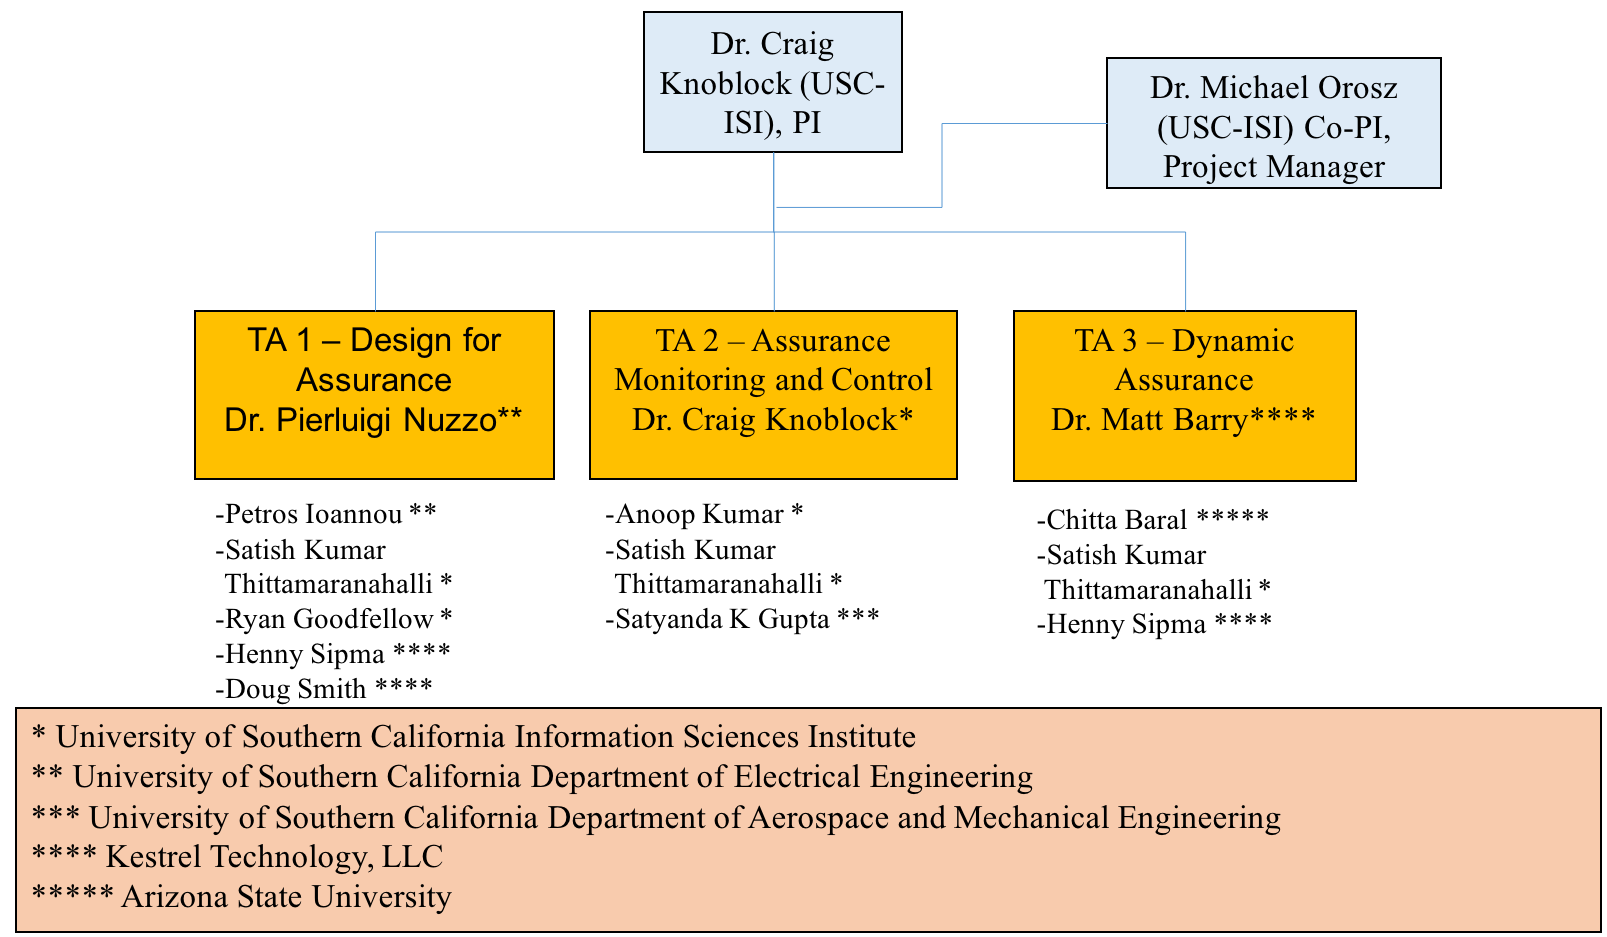
\includegraphics[width=6.0in]{./org-chart2.png}
\caption{\small Organization Chart}
\label{fig:org_chart}
\end{figure}

Coordination: To maximize collaboration and reduce risk to project failure from lack of communication and technical exchange, we plan to employ a wide variety of working styles and communication/coordination so that all can contribute.  At the core of our project will be regularly scheduled meetings bridging the diversely distributed team (Table~\ref{fig:Collaboration_Table}).  These meetings will address project status, identify challenges, implement risk mitigation strategies and participate in technology exchanges and system integration efforts (when appropriate)

\begin{table}[ht]
\caption{\small Project Meetings and Events}
  \centering
  {\footnotesize
\begin{tabular}{|m{3.15in}|m{3in}|} 
\hline
\textbf{Meeting} & \textbf{Frequency} 
\\\hline
Conference calls among investigators (discuss project status, address concerns and project risks) & Weekly
\\
\hline
Technical exchange and coordination meetings using Bluejeans or another videoconference technology & At least twice a month and more frequently as needed
  \\ 
\hline
Face-to-Face meetings (prior to P/I and demonstration meetings) & Every 3 to 6 months and more frequently (especially at the beginning of the project) as needed
 \\\cline{1-2}

\hline
\end{tabular}
}
\label{fig:Collaboration_Table}
\end{table}

\begin{table}[tbhp]
\caption{\small Key Project Team Member Responsibilities}
  \centering
  {\footnotesize
\begin{tabular}{| m{.75in} | m{3.9in}| m{1.5in}|} 
\hline
\textbf{Key Member} & \textbf{Responsibilities} & \textbf{Tasks} 
\\\hline
Dr.\ Craig Knoblock  & Principal Investigator responsible for project, leads TA 2 – Assurance Monitoring and Control.  Will lead the overall project and lead the TA2 team.  Served as the PI on many DARPA projects and has sucessfully led many large teams.    Effort on project:  25\% &
1.1.6, 1.2.2 1.2.3, 1.2.4, 1.3.4, 1.4.1, 
2.1.6, 2.2.2 2.2.3, 2.2.4, 2.3.4, 2.4.1, 
3.1.6, 3.2.2, 3.2.3, 3.2.4, 3.3.4, 3.4.1
\\
\hline
Dr.\ Michael Orosz & Co-Principal Investigator responsible managing the day-to-day operations of the project, assist technical teams as needed, coordinate with TA4 teams.    Has led many large complex multi-disciplined/multi-organizational projects in academic and industry environments.  Effort on project: 50\%
& 1.1.6, 2.1.6, 3.1.6, 1.4.1, 2.4.1, 3.4.1
  \\ 
\hline
Dr.\ Pierluigi Nuzzo 
& 
Co-Principal Investigator.  Leads the TA 1 - Design for Assurance team and conducts research on the formal methods for the design of the TA1 system.  Research experience on methodologies and tools for the design of cyber-physical systems; contracts, interfaces, and compositional methods for embedded system design; the application of automated formal methods and optimization theory to problems in embedded and cyber-physical systems.  Effort on project: 2 months/year (16.6\%)
& 
1.1.1, 2.1.1, 3.1.1 \\
\hline
Dr.\ Matthew Barry
& 
Key personnel.  Leads the TA 3 – Dynamic Assurance.   He will conduct the research on the dynamic assurance case language editors and parsers, the run-time system, and system integrations. Effort on project:  66\%
& 
1.3.2, 2.3.2, 3.3.2\\
\hline
Dr.\ Chitta Baral
& 
Key personnel responsible for learning assurance rules, supporting assurance rules with uncertainty and improving solver speed.  Expertise on ASP solvers, which will be used to reason about the assurance cases. Effort on project: 20\%
& 
1.3.1, 2.3.1, 3.3.1 \\
\hline
Dr.\ Doug Smith 
& 
Key personnel will support formal methods aspects of TA1, and lead the effort on abstract refinement. Expertise in field of automated correct-by-construction program generation.    Effort on project: 40\%
& 
1.1.5, 2.1.5, 3.1.5 \\
\hline
Dr.\ Henny Sipma
& 
Key personnel who will support the program verification tasks under TA1.  Will lead the effort on program verification.   Effort on project:  45\%
& 
1.1.5, 2.1.5, 3.1.5, 1.3.2, 2.3.2, 3.3.2 \\
\hline
Dr.\ Petros Ioannou
& 
Key personnel responsible providing and extending the assurance test bed, which will be available at the start of the project for autonomous vehicles.   Effort on project: 1 month/year (8.3\%)
& 
1.1.2, 2.1.2 (optional), 3.1.2 (optional)
\\
\hline
Dr.\ Satyandra Kumar Gupta
& 
Key Personnel providing autonomous command and control expertise to the TA-2 team.   Will lead the research on safety aware learning on TA2.   Past research on physics-aware decision making to facilitate automation.  Effort on project: 1 month/year (8.3\%)
& 
1.2.1, 2.2.1, 3.2.1 \\
\hline
Dr.\ Anoop Kumar 
& 
Key personnel providing support to the TA 2 project team.  Will lead the research on monitoring \& control and detecting distribution shifts.  Effort on project: 50\%
& 
1.2.1, 1.2.2, 1.2.3, 1.2.4, 2.2.1, 2.2.2, 2.2.3, 2.2.4, 3.2.1, 3.2.2, 3.2.3, 3.2.4\\
\hline
Dr.\ Satish Thittamaranahalli
& 
Key personnel developing scalable algorithms for TA1, TA2, and TA3 project teams.  Has extensive experience on scalable algorithm design, machine learning, and constraint reasoning.  Effort on project: 50\%
& 
1.2.1, 1.2.2, 1.2.3, 1.2.4, 2.2.1, 2.2.2, 2.2.3, 2.2.4, 3.2.1, 3.2.2, 3.2.3, 3.2.4, 1.1.4, 2.1.4, 3.1.4 \\
\hline
Dr.\ Ryan Goodfellow
& 
Key personnel providing support to the TA-1 project. Will lead the research on simulation-based testing.  Has extensive experience on simulation-based testing.  Effort on project:  30\%
& 
1.1.3, 2.1.3, 3.1.3 \\

\cline{1-2}

\hline
\end{tabular}
}
\label{fig:Table_Mgmt}
\end{table}



\newpage
\section{Personnel, Qualifications and Commitment}

{\bf Dr.\ Craig Knoblock}, the PI on this effort, is a Research Professor of both Computer Science and Spatial Sciences at the University of Southern California (USC) and Director of the Intelligent Systems Division at the USC Information Sciences Institute.   He received his Ph.D. from Carnegie Mellon University in computer science. 
%His research focuses on techniques for describing, acquiring, and exploiting the semantics of data.  
In previous projects he has worked on developing  scalable approaches to execution monitoring, accurate detection of sensor failures, and   automatic modeling and reconstruction of sensors.  He has published more than 300 journal articles, book chapters, and conference papers on these topics.  Dr. Knoblock is a Fellow of the Association for the Advancement of Artificial Intelligence (AAAI), a Distinguished Scientist of the Association of Computing Machinery (ACM), a Senior Member of IEEE, past President and Trustee of the International Joint Conference on Artificial Intelligence.
%and winner of the 2014 Robert S. Engelmore Award.  

{\bf Dr.\ Michael Orosz}, a Co-PI on this effort, is a Research Associate Professor of Civil and Environmental Engineering at the University of Southern California (USC) and Research Director of the Decision Systems Group at the USC Information Sciences Institute.  Dr. Orosz has over 30 years’ experience in commercial and government software development, basic and applied research, project management, academic research and has developed and deployed several commercially successful products.  His research interests are in machine learning and decision analytics as applied to intelligence analysis and autonomous command and control such as smart building controls.    Dr. Orosz has extensive experience in managing large complex multi-disciplined/multi-teamed research projects. %funded by DARPA, DHS, DoD, DoE, Industry, NASA, NRO, NSA and ONR.   
He received his Ph.D. in computer science from the University of California, Los Angeles.

{\bf Dr.\ Pierluigi Nuzzo}, a Co-PI on this project, is an Assistant Professor in the Department of Electrical Engineering at the University of Southern California. He received the Ph.D. in Electrical Engineering and Computer Sciences from the University of California at Berkeley. 
%in 2015, and the Laurea degree (MS) in electrical engineering (summa cum laude) from the University of Pisa, Italy, and the Sant'Anna School of Advanced Studies, Pisa, Italy.
%
%He has four years of research experience in analog and mixed signal circuit design as a researcher at IMEC, Leuven, Belgium, and over 10 years experience in design methodologies and tools for mixed-signal integrated circuits and cyber-physical systems, as a researcher at the University of Pisa, IMEC, UC Berkeley, and USC. 
His research interests
include: methodologies and tools for cyber-physical system and mixed-signal
system design; contracts, interfaces and compositional methods for embedded
system design; the application of formal methods and optimization theory to problems in embedded and cyber-physical systems and electronic design automation. 
%
Prof. Nuzzo received %First Place in the operational category and Best Overall
%Submission in the 2006 DAC/ISSCC Design Competition, 
a Marie Curie Fellowship
from the European Union in 2006, 
the University of California at Berkeley EECS
departmental fellowship in 2008, 
%the University of California at Berkeley Outstanding Graduate Student Instructor Award in 2013, 
the IBM Ph.D.
Fellowship in 2012 and 2014, 
%the Best Paper Award from the International Conference on Cyber-Physical Systems (ICCPS) in 2016, 
and the David J.~Sakrison Memorial Prize in 2016 for his doctoral research. 
%He is an author of 1 patent and over 60 publications.

{\bf Dr.\ Satyandra K. Gupta} is Smith International Professor in the Department of Aerospace and Mechanical Engineering at the University of Southern California. %Prior to joining the University of Southern California, he was a Professor in the Department of Mechanical Engineering and the Institute for Systems Research at the University of Maryland. He was the founding director of the Maryland Robotics Center and the Advanced Manufacturing Laboratory at the University of Maryland. 
He served as a program director for the National Robotics Initiative at the National Science Foundation from September 2012 to September 2014.  Dr. Gupta's interest is in the area of physics-aware decision making to facilitate automation. He has published more than 300 technical articles. He is a fellow of the American Society of Mechanical Engineers (ASME) and editor of ASME Journal of Computing and Information Science in Engineering. Dr. Gupta has received the Young Investigator Award from the Office of Naval Research in 2000, CAREER Award from the National Science Foundation in 2001, Presidential Early Career Award for Scientists and Engineers (PECASE) in 2001, Invention of the Year Award at the University of Maryland in 2007, Kos Ishii-Toshiba Award from ASME in 2011, and Excellence in Research Award from ASME in 2013.%, and Distinguished Alumnus Award from Indian Institute of Technology, Roorkee in 2014. %He has also received seven best paper awards at conferences.

{\bf Ryan Goodfellow} is a computer scientist at ISI working in combined cyber physical simulation and emulation platform development. His formal background is in simulation algorithms and modeling techniques using differential-algebraic equations (DAE). He has applied this knowledge in the CPS space by integrating DAE modeling languages and simulation engines with network testbeds to create comprehensive scientific experimentation platforms for cyber-physical systems. These experimentation platforms have been used in the power grid research space. %Ryan is a lead developer on the Deter network testbed, with a strong background in networked and distributed systems engineering. %He is also a combat veteran, serving as a non-commissioned officer and SIGINT team lead for a multi-functional intelligence team in Afghanistan.

{\bf Dr.\ Petros Ioannou} is a Professor in the Department of Electrical Engineering, Director of the Center for Advanced Transportation Technologies and Associate Director for Research for the DOT supported University Transportation Center at USC. He received his MS and PhD from the University of Illinois at Urbana Champaign in Mechanical and Electrical Engineering, respectively. His research interests are in robust adaptive control, vehicle dynamics and control, human factors and safety, automated vehicles, nonlinear systems and Intelligent transportation Systems.  He received the 2016 IEEE Transportation Technologies field award and the 2016 IEEE Control system society Transition to Practice Award. He is a Fellow of IEEE, IFAC and IET and author/coauthor of 8 books and over 400 papers.

{\bf Dr.\ Matthew Barry} will serve as lead for the TA3 tasks. %He will implement the dynamic assurance case language editors and parsers, the run-time system, and system integrations.  He will implement the assurance case arguments and the API for updating argument structure and content.  
Dr. Barry currently is CEO at Kestrel Technology LLC, and previously spent 20 years in NASA space mission operations at the Jet Propulsion Lab and Johnson Space Center.  At NASA Headquarters he led the introduction of dependability case requirements and plans for flight computing systems in upcoming manned space exploration missions, as well as the development of Agency-level software-related safety-critical control system requirements.  He recently served as a Principal Investigator on DHS/Cyber S\&T STAMP (Static Tool Analysis Modernization Program), DARPA CSFV (Crowd Sourced Formal Verification), three NASA Aeronautics R\&D projects, and the AFRL-sponsored Static Analysis of Numerical Algorithms project.  Dr. Barry earned BSME, MS, and PhD degrees in mechanical engineering, and an MBA degree, from Rice University.  

{\bf Dr.\ Henny Sipma} will support the program verification tasks under TA1.  %She is the key person behind the company's {\em KT Advance\/} and {\em KT Transferal\/} static analysis products, and the designer and programmer of the company's core {\em CodeHawk\/} abstract interpretation engine. 
Dr. Sipma currently is the CTO at Kestrel Technology LLC.  She has spent the past 10 years with Kestrel Technology as a static analysis expert; previously developed and taught static analysis techniques as senior research associate at Stanford University for eight years; and developed industrial process controls as an senior systems analyst at Shell.  She has been Principal Investigator or company lead on several recent R\&D projects for Federal agencies, including two projects under the IARPA STONESOUP (Securely Taking On New Executable Software of Uncertain Provenance) program; the DHS Cyber S\&T Gold Standard project; and the DARPA-sponsored STAC (Space-Time Analysis for Cybersecurity) and MUSE (Mining and Understanding Software Enclaves) programs.  Dr. Sipma earned 
%a BS degree in chemistry and an MS degree in chemical engineering at the University of Groningen in The Netherlands, and 
MS and PhD degrees in computer science from Stanford University.  

{\bf Dr.\ Douglas R.\ Smith} will support formal methods aspects of TA1, including the enforcement of safety properties and the generation of monitors.  He is President of Kestrel Technology LLC and Principal Scientist at Kestrel Institute.  He is a Fellow of the American Association of Artificial Intelligence (AAAI) and an ASE Fellow (Automated Software Engineering).  From 1986 to 2000, he taught an advanced graduate course on correct-by-construction software development at Stanford.  
%Dr. Smith has led the development of a series of software synthesis systems, including KIDS (Kestrel Interactive Development System), Specware, Designware, and Planware. 
%Applications domains have included a variety of complex high-performance planners and schedulers for the US Air Force.  He leads current projects on the generation of air mission plans and cyberoperations.  
Other recent projects focused on automated policy enforcement \cite{SmithD0703,SmithD08}, synthesis of secure network protocol codes, and the synthesis of high-performance constraint-solvers\cite{SmithD08c,SmithD13}.  Dr. Smith has over 30 years experience in the field of automated correct-by-construction program generation and has published over 100 papers. He has one patent.  He received the Ph.D. in Computer Science from Duke University% in 1979.  

{\bf Dr. Chitta Baral} is a Professor in the Department of Computer Science and Engineering at Arizona State University. He will support the TA3 efforts on Learning assurance rules, supporting assurance rules with uncertainty and improving solver speed. Dr. Baral has expertise in various aspects of autonomy and Artificial Intelligence. 
He wrote the first book on answer set programming (published by Cambridge University Press) the formal language behind our assurance rules. Some of his other works relevant to this proposal are: goal specification for autonomous systems, automatic construction of control rules for autonomous systems that satisfy given goals, combining machine learning with reasoning in various contexts, including image understanding. %He is the President of KR Inc. He is an associate editor of AIJ and has been an associate editor of JAIR.

{\bf Dr.\ Satish Kumar Thittamaranahalli (T. K. Satish Kumar)} leads the Collaboratory for Algorithmic Techniques and Artificial Intelligence (CATAI) at USC's Information Sciences Institute. He has published over 60 papers on numerous topics in Artificial Intelligence spanning such diverse areas as Constraint Reasoning, Planning and Scheduling, Probabilistic Reasoning, Robotics, Combinatorial Optimization, Approximation and Randomization, Heuristic Search, Model-Based Reasoning, Knowledge Representation and Spatio-Temporal Reasoning. %He %has served on the Program Committees of many international conferences in Artificial Intelligence
He and is a winner of the 2016 Best Robotics Paper Award and the 2005 Best Student Paper Award from the International Conference on Automated Planning and Scheduling. 
Dr. Kumar received his PhD in Computer Science from Stanford University. %In the past, he has also been a Visiting Student at the NASA Ames Research Center, a Postdoctoral Research Scholar at the University of California, Berkeley, a Research Scientist at the Institute for Human and Machine Cognition, a Visiting Assistant Professor at the University of West Florida, and a Senior Research and Development Scientist at Mission Critical Technologies.

\textbf{Dr.\ Anoop Kumar} is a senior computer scientist at USC ISI and has broad expertise in machine learning, statistical modeling, and software engineering.  Dr.\ Kumar is the technical lead on the DARPA RSPACE program and has played a vital role in developing a system that fuses air operations data from multiple sources, maintains world state, and issues warnings. Previously, he led the research and development of the BBN’s election forecasting system for the IARPA OSI program. %Dr.\ Kumar played a significant role in the DARPA DEFT program by developing a model to support integration of output from multiple NLP algorithms. He has contributed at the development to management levels on government research contracts and commercial projects. 
Dr.\ Kumar helped design and develop BBN's commercially available, hosted speech and medical transcription services offering. 

\begin{table}[!tbh]
\begin{footnotesize}
\vspace{-0.1in}

\begin{tabular}{lll}
\begin{tabular}[t]{|l|@{}c@{}|@{}c@{}|@{}c@{}|@{}c@{}|} \hline
Project & Status & \multicolumn{3}{ c| }{Hours} \\ \cline{3-5}
& & P1 & P2 & P3 \\ \hline



\multicolumn{5}{ |c| }{ \textbf{Craig Knoblock} } \\ \cline{1-5}
Safeguard & Pro & 770 & 641 & 641 \\ \cline{1-5}
ELICIT & Cur & 308 & 256 & 120 \\ \cline{1-5}
WTNIC & Cur & 11 & 0 & 0 \\ \cline{1-5}
EFFECT & Cur & 641 & 107 & 0 \\ \cline{1-5}
LinkedMaps & Cur & 203 & 25 & 0 \\ \cline{1-5}
PRINCESS & Cur & 608 & 96 & 0 \\ \cline{1-5}
SCHARP & Cur & 481 & 54 & 0 \\ \cline{1-5}
MINT & Pen & 650 & 534 & 285 \\ \cline{1-5}

\multicolumn{5}{ |c| }{ \textbf{Michael Orosz} } \\ \cline{1-5}
Safeguard & Pro & 1560 & 1300 & 1300  \\ \cline{1-5}
SMC/SY & Cur & 1803 & 0 & 0  \\ \cline{1-5}

\multicolumn{5}{ |c| }{ \textbf{Matthew Barry} } \\ \cline{1-5}
Safeguard & Pro & 2078 & 1690 & 1554 \\ \cline{1-5}
Starlite & Cur & 1840 & 1692 & 0 \\ \cline{1-5}



\multicolumn{5}{ |c| }{ \textbf{Anoop Kumar} } \\ \cline{1-5}
Safeguard & Pro & 1560 & 1300 & 1300 \\ \cline{1-5}

\end{tabular}
&
\begin{tabular}[t]{|l|@{}c@{}|@{}c@{}|@{}c@{}|@{}c@{}|} \hline
Project & Status & \multicolumn{3}{ c| }{Hours} \\ \cline{3-5}
& & P1 & P2 & P3 \\ \hline

\multicolumn{5}{ |c| }{ \textbf{Pierluigi Nuzzo} } \\ \cline{1-5}
Safeguard & Pro & 520 & 433 & 433  \\ \cline{1-5}
Mirage & Cur & 433 & 0 & 0  \\ \cline{1-5}

\multicolumn{5}{ |c| }{ \textbf{Satyandra Gupta} } \\ \cline{1-5}
Safeguard & Pro & 260 & 217 & 217 \\ \cline{1-5}
Human   & Cur & 22 & 0 & 0 \\ \cline{1-5}
Vehicles & Cur & 36 & 0 & 0 \\ \cline{1-5}
Robot & Cur & 116 & 0 & 0 \\ \cline{1-5}
Assembly & Cur & 33 & 0 & 0 \\ \cline{1-5}
Solar & Cur & 4 & 0 & 0 \\ \cline{1-5}

\multicolumn{5}{ |c| }{ \textbf{Petros Ioannou} } \\ \cline{1-5}
Safeguard & Pro & 260 & 217 & 217 \\ \cline{1-5}
CPS & Cur & 130 & 0 & 0 \\ \cline{1-5}

\multicolumn{5}{ |c| }{ \textbf{Ryan Goodfellow} } \\ \cline{1-5}
Safeguard & Pro & 936 & 780 & 780 \\ \cline{1-5}
STEAM & Cur & 416 & 0 & 0 \\ \cline{1-5}


\end{tabular}
&
\begin{tabular}[t]{|l|@{}c@{}|@{}c@{}|@{}c@{}|@{}c@{}|} \hline
Project & Status & \multicolumn{3}{ c| }{Hours} \\ \cline{3-5}
& & P1 & P2 & P3 \\ \hline

\multicolumn{5}{ |c| }{ \textbf{Chitta Baral} } \\ \cline{1-5}
Safeguard & Pro & 659 & 485 & 485 \\ \cline{1-5}
PostdocBP & Cur & 176 & 0 & 0 \\ \cline{1-5}
Languages & Pen & 528 & 264 & 264 \\ \cline{1-5}
CAREER & Pen & 88 & 44 & 44 \\ \cline{1-5}
CHS & Pen & 510 & 255 & 0 \\ \cline{1-5}

\multicolumn{5}{ |c| }{ \textbf{Doug Smith} } \\ \cline{1-5}
Safeguard & Pro & 1222 & 984 & 840 \\ \cline{1-5}
RSPACE & Cur & 342 & 0 & 0 \\ 
\cline{1-5}
PLANX & Cur & 154 & 0 & 0 \\ 
\cline{1-5}
HACCS & Pen & 923 & 769 & 769 \\ 
\cline{1-5}

\multicolumn{5}{ |c| }{ \textbf{Henny Sipma} } \\ \cline{1-5}
Safeguard & Pro & 1372 & 962 & 840 \\ \cline{1-5}
STAC & Cur & 797 & 0 & 0 \\ \cline{1-5}

\multicolumn{5}{ |c| }{ \textbf{Satish Thittamaranahalli} } \\ \cline{1-5}
Safeguard & Pro & 1560 & 1300 & 1300 \\ \cline{1-5}
MapF & Cur & 103 & 103 & 0 \\ \cline{1-5}

\end{tabular}
\end{tabular}

\end{footnotesize}
\caption{Individual commitments of key personnel}
\label{tab:Commitments}
\vspace{-0.2in}
\end{table}

\clearpage
\newpage
\section{Capabilities}


%\subsection{University of Southern California}
USC has strengths in number of areas that are closely related to the proposed work:
\begin{itemize}[itemsep=0pt,leftmargin=*]
\item Dr.\ Nuzzo 
%has over 10-year research experience in embedded system design, from mixed-signal chip design (analog-to-digital converters, frequency synthesizers, software-defined radio), to methodologies and tools for mixed-signal integrated circuits and Cyber-Physical Systems (CPSs), and the application of formal methods and optimization theory to problems in embedded and cyber-physical systems and electronic design automation.  
%His doctoral work 
has done extensive research on contracts and compositional methods for heterogeneous system design and design space exploration, with application to aircraft electric power systems and environmental control systems. His work has helped transition rigorous system design foundations, innovative design methodologies, and new systems engineering paradigms to industry (IBM, United Technologies). 
\item Dr.\ Satyandra K. Gupta has worked on autonomous surface vehicles, autonomous ground vehicles for operation on rugged terrains, and autonomous flapping wing aerial vehicles.   His group has developed a hierarchal decision making approach for realizing autonomous systems. 
%This approach combines task planning and assignment, deliberative trajectory planning, reactive collision avoidance behaviors, and trajectory tracking control layers. 
His group has also developed new methods for learning reactive behaviors in adversarial environments and COLREGS compliant trajectory planning. \item Dr.\ Knoblock has developed methods that learn the relationships between sensors to both identify failures and changes in sensor and reconstruct those sensors, providing estimates of the accuracy of the reconstructed sensors.  
\item Ryan Goodfellow has extensive experience in simulation based testing through high-fidelity CPS testbed environment development and operation, using the Deter network testbed as the core which has supported several large scale government projects from a variety of agencies and thousands of users. %we have developed sophisticated CPS experiments under programs such as NFS RIPS, NIST SmartCities and the DHS Cybersecurity showcase.
\item Dr.\ Ioannou %helped  design and implement adaptive cruise control systems in collaboration with Ford Motor Company, which was commercialized four years before any other company. He 
worked on several DOT funded projects on automated vehicles and intelligent highway systems where he demonstrated his vehicle control designs for safety and performance on actual automated vehicles in test trucks and I-15 highway.
\item Drs.\ Knoblock, Kumar, and Thittamaranahalli have developed highly scalable approaches for monitoring message traffic to identify potential problems and issue warnings and alerts. 
\item Dr. Thittamaranahalli has developed state-of-the-art methods for efficiently solving large-scale search and optimization problems. %These techniques will be applicable in TA2 for safety-aware learning and planning, in TA2 for assurance monitoring and control, and in TA3 for dynamic assessment of assurance cases.

\end{itemize}
%\subsection{Kestrel Technology LLC}

Kestrel Technology's strength is in program analysis, specifically static analysis of both source and binary targets.  The company performs applied R\&D and product development for a variety of static analysis applications  pivoting primarily on the abstract interpretation technique.  The company recently initiated development of program analysis applications using logical equivalence techniques. As a provider of verification evidence in the form of mathematical proofs, the company also has expertise in the design and development of assurance case arguments for high-integrity systems using such evidence. %The company is engaged in a partnership with Wind River Systems to develop program analysis tools for its embedded system developers.  Many of Wind River's customers must develop their products under safety and certification standards, including those using safety cases.  

   

%\subsection{Arizona State University}
Chitta Baral at Arizona State University has developed various software to learn assurance rules and various ASP solvers, which he has made available as open-source.

Most of the software carried forward for implementation or derivation is open source.  The single exception is Kestrel Technology's {\it KT Advance\/} static analysis tool (TA1), in particular the abstract interpretation engine therein, which is company proprietary and is US EAR export-controlled.   
%Owing to mixed funding for the development of that technology 
We will continue to provide the Federal government a restricted use license for that particular item.

There are no specialized facilities, data, or GFE required for this effort. 

\include{sow}
\include{milestones}

% \section{Level of Effort by Task \textcolor{red}{[Mike/Lisa - 1 pages]}}

% \textcolor{blue}{
% \begin{itemize}
% \item Will be a separate spreadsheet
% \item
% \end{itemize}
% }

\include{appendix_a}

%\section{Appendix B \textcolor{red}{[No Page Count]}}

\section{References}
\bibliographystyle{acm} 
\bibliography{TA3/ta3,TA2/ta2,TA1/ta1}
\end{document}
%%\documentclass[a4paper]{article}
%\documentclass[12pt]{article}
\documentclass[12pt]{dod-blank}

%% Language and font encodings
\usepackage[english]{babel}
\usepackage[utf8x]{inputenc}
\usepackage[T1]{fontenc}

%% Sets page size and margins
%%\usepackage[a4paper,top=3cm,bottom=2cm,left=3cm,right=3cm,marginparwidth=1.75cm]{geometry}
%\usepackage[top=1in, bottom=1in, left=1in, right=1in]{geometry}



%% Useful packages
\usepackage{amsmath}
\usepackage{graphicx}
  \graphicspath{{.}{./image/}}
  \DeclareGraphicsExtensions{.png,.jpg} 
\usepackage[colorinlistoftodos]{todonotes}
\usepackage[colorlinks=true, allcolors=blue]{hyperref}
\usepackage{tabularx}
\usepackage{multirow}
\usepackage{tabulary}
\usepackage{float}
\usepackage{wrapfig}
\usepackage[export]{adjustbox}
\usepackage{comment}
\usepackage{tabularx}
\usepackage{multirow}
\usepackage{tabulary}
\usepackage{enumitem}

\usepackage{listings}
\usepackage{color}
\usepackage{array}
\usepackage{subcaption}
\usepackage{xcolor}




\renewcommand{\textfraction}{0}
\renewcommand{\topfraction}{1.0}
\renewcommand{\bottomfraction}{1.0}

\usepackage{longtable}
%% macros
\newif\iffinal
\finaltrue
\iffinal
  
    \newcommand\baareq[1]{}
    \newcommand\baades[1]{}
 
 
\else
    \definecolor{darkgreen}{rgb}{0,0.4,0}
    \definecolor{darkcyan}{rgb}{0,0.4,0.4}
    \definecolor{darkblue}{rgb}{0,0,0.5}
    
    \newcommand\baareq[1]{{\color{darkcyan}[\textbf{Requirement:} #1]}}
    \newcommand\baades[1]{{\color{darkcyan}[\textbf{Description:} #1]}}
 
\fi




\def\naive{na\"{\i}ve}



\lstset{ 
  backgroundcolor=\color{white},   % choose the background color; you must add \usepackage{color} or \usepackage{xcolor}
  basicstyle=\footnotesize\ttfamily,            % the size of the fonts that are used for the code
  breakatwhitespace=false,         % sets if automatic breaks should only happen at whitespace
  breaklines=true,                 % sets automatic line breaking
  captionpos=b,                    % sets the caption-position to bottom
  commentstyle=\color{mygreen},    % comment style
  % deletekeywords={...},            % if you want to delete keywords from the given language
  escapeinside={\%*}{*)},          % if you want to add LaTeX within your code
  extendedchars=true,              % lets you use non-ASCII characters; for 8-bits encodings only, does not work with UTF-8
  frame=single,	                   % adds a frame around the code
  keepspaces=false,                 % keeps spaces in text, useful for keeping indentation of code (possibly needs columns=flexible)
  keywordstyle=\color{blue}\bfseries\underbar,       % keyword style
  language=Prolog,                 % the language of the code
  % morekeywords={if,and},        % if you want to add more keywords to the set
  numbers=none,                    % where to put the line-numbers; possible values are (none, left, right)
  numbersep=5pt,                   % how far the line-numbers are from the code
  numberstyle=\tiny\color{mygray}, % the style that is used for the line-numbers
  rulecolor=\color{black},         % if not set, the frame-color may be changed on line-breaks within not-black text
  showspaces=false,                % show spaces everywhere adding particular underscores; it overrides 'showstringspaces'
  showstringspaces=false,          % underline spaces within strings only
  showtabs=false,                  % show tabs within strings adding particular underscores
  stepnumber=2,                    % the step between two line-numbers. If it's 1, each line will be numbered
  stringstyle=\color{mymauve},     % string literal style
  tabsize=2,	                   % sets default tabsize to 2 spaces
  title=\lstname                   % show the filename of files included with \lstinputlisting; also try caption instead of title
}

% apply trick for additional keywords for our AC DSL
\lstset{
	emph={for, if, and, or},
    emphstyle={\color{blue}\bfseries\underbar}
}




\title{DARPA Assured Autonomy}
\author{Technical Volume- \textcolor{red}{Thirty-Eight (38) pages max}}

\begin{document}
\pagenumbering{roman}
\include{cover}

\newpage
\section{Table of Contents}
\tableofcontents

\newpage
\pagenumbering{arabic}
\section{Executive Summary}
As we rapidly move into a world where machine learning plays a central role in realizing autonomous systems, it is becoming increasingly important to develop techniques that assure that these systems will operate safely and perform as expected. Current approaches are limited to providing assurance for systems with limited or no  learning capabilities. In this context, DARPA's Assured Autonomy BAA seeks to \emph{develop rigorous design and analysis technologies for continual assurance of learning-enabled autonomous systems}. USC in collaboration with Kestrel Technology and ASU is pleased to submit a comprehensive TA1, TA2, and TA3 proposal entitled \emph{``Assured Autonomy for Learning Enabled Vehicles (Safeguard).''} We plan to provide an end-to-end solution to support autonomous systems with learning-enabled components, ranging from design technologies for assurance, to assurance monitoring and control techniques, to representation and online evaluation of assurance cases. We have assembled a strong team of experts that cover the range of technologies that are required to create such an end-to-end system. If successful, the project will provide the technologies for building the next-generation of learning-enabled autonomous systems.  The entire project will take four years and cost \textcolor{red}{\$??}, with an initial version completed at the end of Phase I and successive versions with additional capabilities and improved scalability at the end of Phase II and Phase III.  

In the remainder of this section, we first introduce an  unmanned surface vehicle scenario that will be used throughout the proposal to describe the approach.  Next, we describe our approach to design, monitoring, and dynamic assurance. Finally, we introduce the team involved in the project. 

\textbf{Motivating Scenario.} Consider an autonomous unmanned surface vehicle (USV) guarding a valuable asset in the ocean when an unknown vehicle  approaches the security perimeter, under challenging weather conditions. In this scenario, the USV is required to approach the intruding vehicle, issue a warning signal, and escort it to a safe distance from the controlled area. However, as the USV has no a priori knowledge of its external environment behaviors (e.g., water depth, waves, wind, current, visibility), pre-computing a feasible trajectory, let alone optimal, becomes a non-trivial problem. For trajectory planning, the USV must continuously perform the following tasks:
\begin{itemize}[itemsep=0pt,leftmargin=*]
 \item Sense the current state of the surrounding environment (e.g., water depth, waves, wind, current, visibility) and estimate its own maneuverability constraints (e.g., braking distance, available acceleration, maximum velocity, turning radius, turning rate, safety distance) based on the state of the environment;      
\item Sense the static obstacles in the sensor range and generate a traversability map;
\item Sense the moving obstacles and classify them;   
\item Predict future trajectories of moving obstacles; 
\item Determine if any of the COLREGS \cite{commandant1999international} rules will be in effect with respect to one or more of the nearby vessels and identify the vessels with the right of way.    
\end{itemize}
The above information will be used by the trajectory planner to compute an initial trajectory, which will be continuously refined as the USV gathers additional information.
% It is not possible for the USV to be tested in every possible environment. 
The USV will use learning enabled components to take  decisions as it encounters new situations, such as  
\begin{itemize}[itemsep=0pt,leftmargin=*]
\item Classifiers to identify moving obstacles based on physical appearance and motion signatures,
\item Algorithms to estimate the sensor capabilities in adverse weather conditions,   
\item Algorithms to accurately estimate uncertainty in the environment, 
\item Classifiers to generate traversability maps,
\item Prediction of external vessel behaviors based on motion histories, 
\item Reinforcement learning  to ensure COLREGS compliance of maneuvers,  
\item Algorithms to learning pursuit behaviors.  
\end{itemize}
Learning enabled components will interact with each other in complex ways, where a misclassification error in one component may eventually compromise the entire mission.   
% We will need to make sure that each learning enabled components has a run-time monitor that will ensure that the assumptions made by the learning-enabled component remain valid and prevent erroneous learning. 
% For example, if the vehicle is exhibiting significant error in trajectory tracking, then simply downgrading the trajectory tracking error value may not be a good option.  The failure of prediction of trajectory tracking error might be due to the presence of a significant wake caused by a nearby vessel. The presence of the nearby vessel can be used to explain the degradation in trajectory tracking performance. As the vessel moves away, we can expect the trajectory tracking performance to return to the predicted level.  
While exhaustive validation of learning-enabled cyber-physical systems (LE-CPSs) is a prohibitive task~\cite{Kalra16},
their complexity, heterogeneity, and highly dynamic nature
make it challenging to even leverage existing model-based development techniques to effectively assess system correctness 
% dependability, 
at design time or enforce it at runtime.

\textbf{Design for Assurance.} Safeguard uses a platform-based design approach~\cite{Nuzzo15b} to organize the design process for a LE-CPS and to build assurance cases. Composite models are developed at several levels of abstraction,
from top-level system requirements and safety constraints down to the
implementation level.  Intermediate levels add detail to the levels
above.  The different levels are connected by refinement mappings that
allow properties established at one level to be preserved at the next
level (see Figures~\ref{fig:methodology} and~\ref{fig:assurance}).

Contracts are used to formally specify components and composite models
in terms of (1) Assumptions -- the assumed behaviors of the
environment and the behaviors of other components, and (2) Guarantees
-- the behavior properties that a model guarantees if it operates in a
context that satisfies its assumptions.  A calculus of contracts
allows horizontal composition of contracts to generate contracts for
composite models.  Vertical contracts are used to specify the mapping
or refinement relation between models at different levels of
abstraction.  The system design process starts with a high-level
contract that expresses overall system assumptions and requirements.
Subsequent levels express models with increasing detail until the
lowest level expresses the system in terms of hardware components and
their software controllers.

The assurance case for a CPS arises from the horizontal and vertical
structure of the design in several ways.  The components used within a
particular level are either (1) synthesized using
correct-by-construction design tools together with proofs, (2) derived
statically or dynamically using safety-aware machine-learning
techniques, (3) written manually and verified by analysis tools, or
(4) written manually and validated by extensive testing.  The
assurance case for the whole reflects its compositional structure.  We
anticipate that well-specified contracts together with the calculus of
contracts will eliminate well-known problems with unexpected emergent
behaviors in CPS systems.

The assurance case for the lowest-layer design arises from both the
intra-level assurance and from properties and their proofs that are
preserved under the refinement mapping from the top-level
requirements.  The refinement mappings between model layers will be
constructed using a variety of techniques.  A contract at an abstract
level can be mapped to a component or refined contract by (1)
retrieval of pre-verified components from a platform library, (2)
synthesis using correct-by-construction design and optimization tools,
or (3) manual coding to satisfy a contract.  The mapping of a
composite model will be composed from the mappings of its constituent
components or contracts.  When a composite model cannot be mapped
compositionally to the next level, it will be generated using
correct-by-construction design and optimization tools.

\textbf{Assurance Monitoring and Control.}
We provide an integrated framework for safety-aware learning, assurance monitoring and control, detecting distribution shifts. Three major components offer an efficient TA2 architecture as well as interfaces with TA1 and TA3, that is, (a) safety-aware learning and planning, (b) assurance monitors for guarding architectural and safety constraints; and (c) distribution shift detection.

We will develop a new learning-enabled online decision-making framework that allows opportunistically composing a sequence of actions (maneuvers) to reduce uncertainty in the system capability model without suspending the progress toward the mission goals or compromising safety. Each candidate action is evaluated based on three criteria: (1) the risk of violating a safety constraint using the current uncertainties in the parameter estimates; (2) its relevance to the mission goals; (3)  its expected information gain, i.e., reduction in uncertainty, with respect to the parameter estimates. These evaluations are combined to produce a cumulative mission utility value for each action that drives our learning-enabled decision-making framework. The problem of generating and evaluating sequences of actions can be posed in several way. For example, it can be solved using a branch-and-bound search method like Anytime A*, or formulated with the finite-horizon Markov Decision Process (MDP) framework. We will develop new scalable search strategies to solve this problem efficiently, by potentially evaluating a recent method developed at USC, called FastMap, that can significantly improve the execution time. 

We will develop monitors for architectural and safety constraints. 
% While these constraints can be checked over and over again as sensor information flow in, this naive strategy accounts for a lot of computational overhead. 
To achieve scalability and decrease the overhead, we propose the application of a technique that we currently use in DARPA's RSPACE program, which leverages a physical model of the vehicles dynamics and its interactions with the environment to efficiently determine the readout frequency. We propose two  extensions of this basic idea. First, we will use the theory of Variable Elimination to prioritize which variables to monitor, e.g., controllable, versus uncontrollable, adversarially controlled, or unobservable variables. Second, we invoke the dynamic assessment of assurance cases only when needed. This  decreases the number of times dynamic assessment of assurance cases is initiated as well as the communication bandwidth between the TA2 and TA3 components.

Finally, we will identify a distribution shift by combining statistical and machine learning techniques to differentiate between environmental and sensor changes. We will exploit a categorization of the shifts based on their cause and duration as well as extend our earlier work on detecting and mitigating sensor failures for all types of monitored variables.  

\textbf{Dynamic Assurance:} The Safeguard {\em design for assurance\/} activity takes a systems-theoretic stance toward safety.  Consequently, it presumes that safety is an emergent property of the system, and that hazards can present themselves through unintended interactions and performance violations in addition to causal events such as component failures.  Our design approach includes consideration of intent as well as hazard analysis and mitigation.  The artifacts from these activities populate contracts and assumptions for the dynamic assurance case.  
We thus build safety into the product by working at a systems-level viewpoint, using lexicon and design patterns familiar to both hardware and software engineers; safety is an emergent property of the system, not an afterthought.  
As system behavior evolves during runtime owing to learning, threats, degradation, or some other factor, the dynamic assurance case identifies whether the safety constraints continue to be satisfied.  If not, it provides notifications or issues recovery instructions directly from a lookup table.

Our implementation of the dynamic assurance case employs a declarative knowledge base inference engine and a domain-specific language tailored to our approach.  We have used them successfully for assurance case tool sets and arguments, and will extend them to reason about uncertainty and learning.  Our approach to achieve scalability is to specialize solvers toward modularity and to take advantage of domain knowledge.  Specifically, we will develop answer set programming techniques for context-dependent learning for reasoning about the learning-enabled components as well as learning assurance rules.  We will develop new formalisms for uncertainty to include causality, using weights for computing probabilities, and probabilistic non-monotonicity.  To achieve scaling objectives we will implement specializations using modularity, weighted CSPs, and message passing. 

% The system safety constraints revealed from that design become the key elements of our dynamic assurance case.  Our verification tools ensure the constraints are relevant, identifiable, and their implementation and effect observable.  

\textbf{Team.} We have assembled a team that is exceptionally well-qualified to build the proposed Safeguard system.  The team will be led by Dr.\ Craig Knoblock, the Principal Investigator for the effort, who currently leads the Intelligent Systems Division at the Information Sciences Institute.  He has led many large DARPA and IARPA projects over the years and has a strong track record in conducting leading edge research and then transitioning the technology to commercial use.  He will be supported by Dr.\ Michael Orosz as the Project Manager, who also has  experience in managing large research projects and on autonomous systems.  The TA1 team will be led by Dr.\ Pierluigi Nuzzo, who is an expert in embedded system design methodologies and the  application of formal methods to cyber-physical systems.  The TA1 team also includes Dr.\ Doug Smith, who has spent many years working on scalable correct-by-construction techniques and Dr.\ Henny Sipma, who has significant experience in applying program verification methods to real-world problems.  The TA1 team also includes Ryan Goodfellow, who has done a large amount of work on simulation-based testing.  The TA2 team will be led by Dr.\ Knoblock who has worked on topics related to both monitoring and detecting distribution changes.  He will be supported by Dr.\ Satyandra Gupta, who is an expert on autonomous surface vehicles as well as on safety-aware learning. He will also be supported by Drs.\ Anoop Kumar and Satish Thittamaranahalli, who have also previously worked on efficient methods for execution monitoring.  The TA3 team will be lead by Dr.\ Matthew Barry, who has experience in creating the technologies for assurance cases.  He will be supported by Dr.\ Chitta Baral, who is an expert on ASP solvers and by Dr.\ Thittamaranahalli who is an expert on SAT solvers, both of which will be applied to provide scalable assurance case reasoning.  Finally, Dr.\ Petros Ioannou, who is an expert on control systems for autonomous vehicles will provide an autonomous vehicle platform, which will form the focus of our work until the TA4 teams provide additional vehicle platforms for development.  

\newpage
\section{Innovative Claims and Deliverables}

In this project we will develop and build an end-to-end system for assured autonomy.  This section describes the key innovations by technical area and then the overall deliverables of the project.

\paragraph{Design for Assurance}

\begin{itemize}[itemsep=0pt,leftmargin=*]
\item We address the LE-CPS design challenges via a holistic approach that can contextually generate design artifacts and assurance cases. We develop a compositional, contract-based modeling framework, methods, and tools to support the design process from system-level requirement capture,  formalization, and analysis, to the generation, testing, and continual monitoring of software and hardware artifacts in feedback loop with a physical process.

\item We develop compositional abstractions and interfaces (vertical contracts) that can  bridge heterogeneous formalisms and heterogeneous decomposition architectures to make system analysis and synthesis tractable, consistently combine different verification and synthesis methods at design time, and provide seamless support for dynamic assurance at run time. %We aim to quantitatively capture the confidence in the satisfaction of requirements under uncertain or unknown conditions, and resilience properties of  systems at different abstraction levels, to enable trade-off evaluation between resilience, performance, and cost.

\item We develop a unifying framework and efficient algorithms to reason about the combination of discrete and continuous dynamics and constraints in the presence of uncertainties in LE-CPS using a satisfiability modulo convex approach~\cite{Shoukry2017} for contract-based system verification and scalable trajectory planning.  

\item We provide an environment for high-fidelity CPS testing, in which production-ready software, e.g.,  safety-critical learning and control, may be deployed and tested 
% by extending the Cypress testbed environment \cite{Goodfellow2015Cypress:Systems} 
with time dilation facilities, so that it synchronizes with a physical simulation that is not necessarily running in real time, while still having the perception of real time.

\item We 
% These facilities allow a cyber system to be  
propose an approach for unanticipated behavior space identification and test coverage maximization which leverages results from the theory of differential algebraic equation (DAE)~\cite{Berger2013ControllabilitySurvey,Ilchmann2005ATheory,BergerOnSystems,Lamour2013} 
to prune the behavior search space and identify smaller regions of interest for efficient simulation-based testing. 
% We then compute the intersection of these two behavior spaces and restrict our simulation based testing search space to this subspace.
\end{itemize}

\paragraph{Assurance Monitoring and Control}

\begin{itemize}[itemsep=0pt,leftmargin=*]
\item 
%We integrate safety-aware learning into the overall decision making problem. The goal is to maximize mission utility without violating the safety constraints. 
Our safety-aware learning framework enables the system to opportunistically select and execute actions to assist the learning-enabled component in reducing model uncertainty without compromising safety or deviating from the mission goals. The value of uncertainty reduction is explicitly incorporated in the optimization process for selecting the best action.  
\item For safety-aware learning, we propose the idea of preprocessing the search space of the problem domain before queries and observations come in. With such a linear-time preprocessing phase, the performance of search and optimization algorithms can be significantly boosted. For example, in regular A* search, the intensional or extensional search space can be preprocessed in near-linear time to yield an embedding of each state as a point in Euclidean space~\cite{cujakk}. Then, when the query comes in, A* search can make use of these Euclidean distances as heuristic distances between two states to yield order-of-magnitude speedups. 
%In Anytime A* for safety-aware learning and planning, this leads to a significantly better quality of actions chosen within a time limit, and in the MDP framework, the same ideas can be used to improve the convergence of Bellman updates for safety-aware Reinforcement Learning.
\item As massive amounts of sensor information flow in, it is imperative for us to efficiently process this information for monitoring architectural and safety constraints. Building on our past work on similar tasks, we propose novel technologies for efficiently monitoring constraints. These algorithms can yield an exponential reduction in the amount of sensor data that needs to be processed. Doing this also reduces the message complexities between the various modules. %We also propose to use the theory of Variable Elimination (VE) to monitor constraints with uncontrollable, adversarially controlled, and/or unobservable variables. VE yields a substrate constraint to monitor that characterizes a dominant strategy of the controllable variables over the uncontrollable, adversarially controlled, and/or unobservable variables.
\item We will develop techniques to identify  distributional shifts and determine the underlying cause (e.g., change in environment, sensor failure,   etc.), as well as strategies for handling the various distributional shifts.   Notably, we propose to build on our past work and use compact representations to exploit historical data to identify distributional shifts.
\end{itemize}

\paragraph{Dynamic Assurance}

\begin{itemize}[itemsep=0pt,leftmargin=*]

\item We demonstrate the integration of dynamic assurance for safety-critical learning-enabled dynamic systems in which evolutionary behaviors are expected and tolerated as a property of the functionality.   The impact will be consequential contributions safety-critical dynamic systems in which evolutionary behaviors are expected and tolerated as portion of the functionality.   
\item We implement dynamic assurance by combining features of system safety, formal methods, logic programming, uncertain reasoning, and domain-specific languages.  We populate assurance case arguments at several levels of modeling and implementation abstraction, using the analysis results to produce design-time evidence supporting assurance claims.  
%We provide automated reasoning about the assurance case itself to produce verification, consistency, and completeness results for the argument.  Dynamic assurance results then yield trusted explanations of whether safety constraints and assumptions and other contracts still hold during the collection of runtime evidence from monitors. 
\item We develop and demonstrate ASP formalisms crucial to applications in dynamic assurance. We demonstrate the suitability of the technology especially for assurance case arguments owing to the improved legibility, consistency and completeness checks, handling of uncertain and default reasoning, and scalability.  
%We will produce modularized solvers for enhanced performance based on recent algorithmic developments in exploiting structure, kernelization, and message passing. We provide a formalism to enable learning of assurance rules. 
We provide a novel approach to handling uncertainty that provides the ability to do causal and counter-factual reasoning as well as probabilistic non-monotonicity.  Overcoming limitations of traditional inductive logic techniques, we develop a novel iterative and incremental approach based on context dependent learning. 
\end{itemize}

\paragraph{Deliverables}
During the course of this project, we will build and deliver a fully-operational system that covers all three of the technical areas.  The detailed capabilities of this system are described in the individual technical sections.  The resulting system will be available as open source under a permissive license, which will allow other organizations to use the work, extend it in new directions, and even commercialize the software.  Kestrel Technology has significant experience in this space and has built and applied these types of technologies to a variety of real world tasks.  Kestrel is ideally suited to pursue commercial uses of this technology and the permissive license will facilitate exploring these opportunities since there will be no need to negotiate intellectual property rights.  

\newpage
\section{Technical Plan}
\input{./TA1/main}
\input{./TA2/main}
\input{./TA3/main}
\clearpage
\newpage


\section{Management Plan}


The Principal Investigator for this effort is Dr. Craig Knoblock who is responsible for all aspects of the effort, will coordinate the parallel team efforts, and will ensure high levels of performance from individual team members.  The Co-P/I, Dr. Michael Orosz, will provide project management and will assist all performers in the execution of the project.    The project team is divided into three working groups (Figure~\ref{fig:org_chart}) corresponding to Technical Areas 1-3, however, members of each team contribute across all project activities.   Table~\ref{fig:Table_Mgmt} defines the major contributions of each project team member to the project tasks.

\begin{figure}[tbhp]
%\vspace{-25pt}
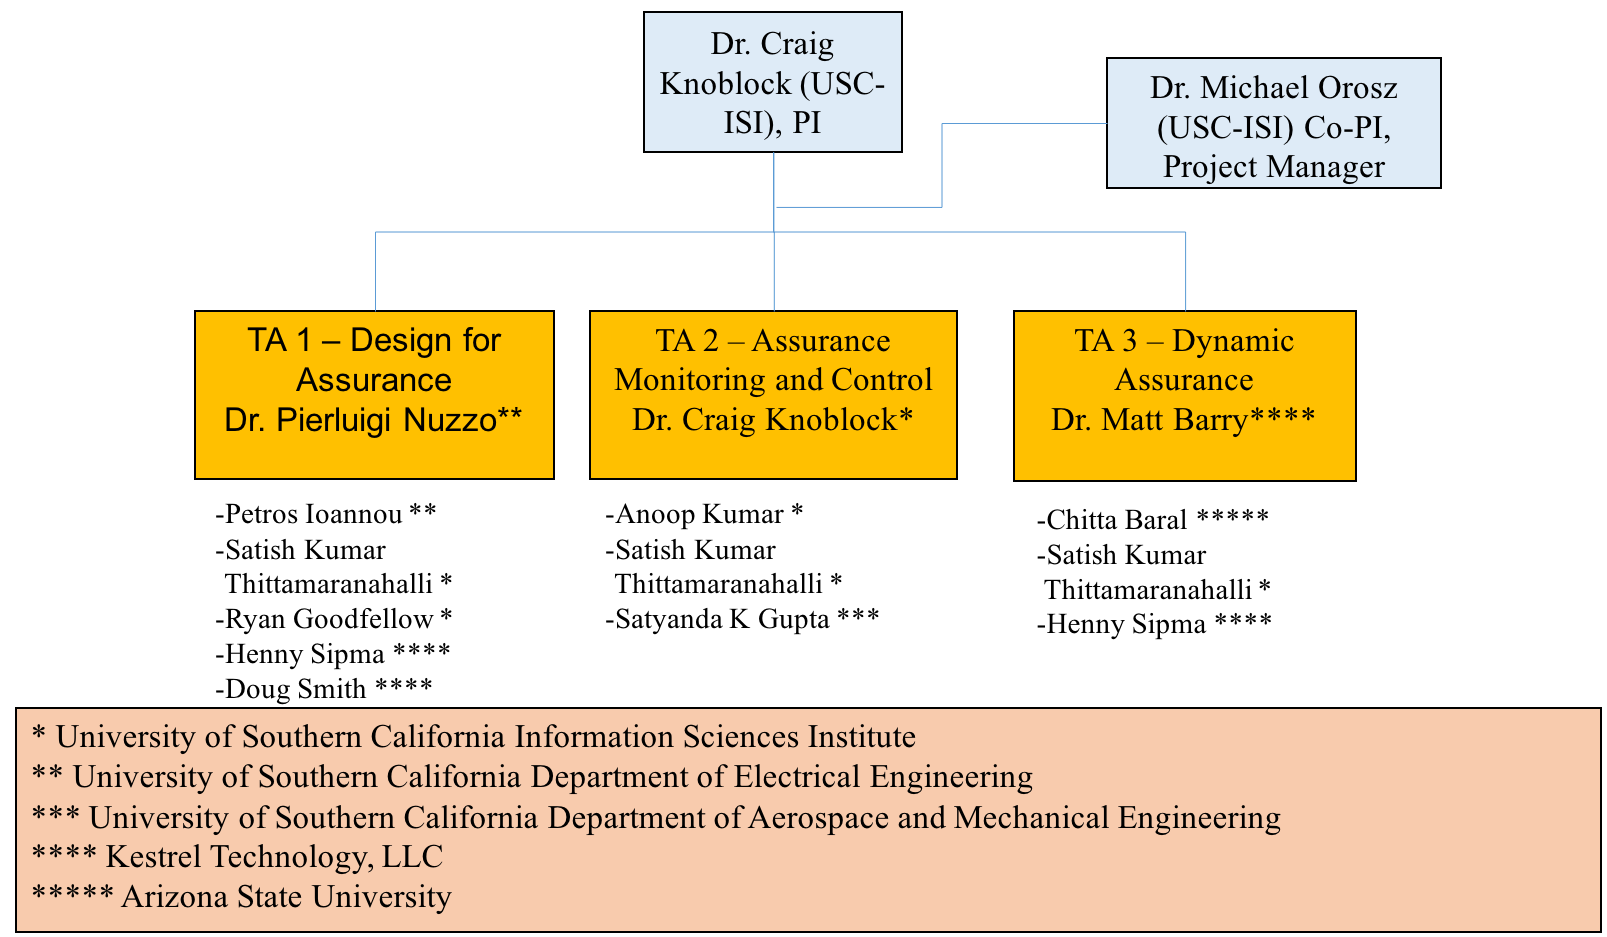
\includegraphics[width=6.0in]{./org-chart2.png}
\caption{\small Organization Chart}
\label{fig:org_chart}
\end{figure}

Coordination: To maximize collaboration and reduce risk to project failure from lack of communication and technical exchange, we plan to employ a wide variety of working styles and communication/coordination so that all can contribute.  At the core of our project will be regularly scheduled meetings bridging the diversely distributed team (Table~\ref{fig:Collaboration_Table}).  These meetings will address project status, identify challenges, implement risk mitigation strategies and participate in technology exchanges and system integration efforts (when appropriate)

\begin{table}[ht]
\caption{\small Project Meetings and Events}
  \centering
  {\footnotesize
\begin{tabular}{|m{3.15in}|m{3in}|} 
\hline
\textbf{Meeting} & \textbf{Frequency} 
\\\hline
Conference calls among investigators (discuss project status, address concerns and project risks) & Weekly
\\
\hline
Technical exchange and coordination meetings using Bluejeans or another videoconference technology & At least twice a month and more frequently as needed
  \\ 
\hline
Face-to-Face meetings (prior to P/I and demonstration meetings) & Every 3 to 6 months and more frequently (especially at the beginning of the project) as needed
 \\\cline{1-2}

\hline
\end{tabular}
}
\label{fig:Collaboration_Table}
\end{table}

\begin{table}[tbhp]
\caption{\small Key Project Team Member Responsibilities}
  \centering
  {\footnotesize
\begin{tabular}{| m{.75in} | m{3.9in}| m{1.5in}|} 
\hline
\textbf{Key Member} & \textbf{Responsibilities} & \textbf{Tasks} 
\\\hline
Dr.\ Craig Knoblock  & Principal Investigator responsible for project, leads TA 2 – Assurance Monitoring and Control.  Will lead the overall project and lead the TA2 team.  Served as the PI on many DARPA projects and has sucessfully led many large teams.    Effort on project:  25\% &
1.1.6, 1.2.2 1.2.3, 1.2.4, 1.3.4, 1.4.1, 
2.1.6, 2.2.2 2.2.3, 2.2.4, 2.3.4, 2.4.1, 
3.1.6, 3.2.2, 3.2.3, 3.2.4, 3.3.4, 3.4.1
\\
\hline
Dr.\ Michael Orosz & Co-Principal Investigator responsible managing the day-to-day operations of the project, assist technical teams as needed, coordinate with TA4 teams.    Has led many large complex multi-disciplined/multi-organizational projects in academic and industry environments.  Effort on project: 50\%
& 1.1.6, 2.1.6, 3.1.6, 1.4.1, 2.4.1, 3.4.1
  \\ 
\hline
Dr.\ Pierluigi Nuzzo 
& 
Co-Principal Investigator.  Leads the TA 1 - Design for Assurance team and conducts research on the formal methods for the design of the TA1 system.  Research experience on methodologies and tools for the design of cyber-physical systems; contracts, interfaces, and compositional methods for embedded system design; the application of automated formal methods and optimization theory to problems in embedded and cyber-physical systems.  Effort on project: 2 months/year (16.6\%)
& 
1.1.1, 2.1.1, 3.1.1 \\
\hline
Dr.\ Matthew Barry
& 
Key personnel.  Leads the TA 3 – Dynamic Assurance.   He will conduct the research on the dynamic assurance case language editors and parsers, the run-time system, and system integrations. Effort on project:  66\%
& 
1.3.2, 2.3.2, 3.3.2\\
\hline
Dr.\ Chitta Baral
& 
Key personnel responsible for learning assurance rules, supporting assurance rules with uncertainty and improving solver speed.  Expertise on ASP solvers, which will be used to reason about the assurance cases. Effort on project: 20\%
& 
1.3.1, 2.3.1, 3.3.1 \\
\hline
Dr.\ Doug Smith 
& 
Key personnel will support formal methods aspects of TA1, and lead the effort on abstract refinement. Expertise in field of automated correct-by-construction program generation.    Effort on project: 40\%
& 
1.1.5, 2.1.5, 3.1.5 \\
\hline
Dr.\ Henny Sipma
& 
Key personnel who will support the program verification tasks under TA1.  Will lead the effort on program verification.   Effort on project:  45\%
& 
1.1.5, 2.1.5, 3.1.5, 1.3.2, 2.3.2, 3.3.2 \\
\hline
Dr.\ Petros Ioannou
& 
Key personnel responsible providing and extending the assurance test bed, which will be available at the start of the project for autonomous vehicles.   Effort on project: 1 month/year (8.3\%)
& 
1.1.2, 2.1.2 (optional), 3.1.2 (optional)
\\
\hline
Dr.\ Satyandra Kumar Gupta
& 
Key Personnel providing autonomous command and control expertise to the TA-2 team.   Will lead the research on safety aware learning on TA2.   Past research on physics-aware decision making to facilitate automation.  Effort on project: 1 month/year (8.3\%)
& 
1.2.1, 2.2.1, 3.2.1 \\
\hline
Dr.\ Anoop Kumar 
& 
Key personnel providing support to the TA 2 project team.  Will lead the research on monitoring \& control and detecting distribution shifts.  Effort on project: 50\%
& 
1.2.1, 1.2.2, 1.2.3, 1.2.4, 2.2.1, 2.2.2, 2.2.3, 2.2.4, 3.2.1, 3.2.2, 3.2.3, 3.2.4\\
\hline
Dr.\ Satish Thittamaranahalli
& 
Key personnel developing scalable algorithms for TA1, TA2, and TA3 project teams.  Has extensive experience on scalable algorithm design, machine learning, and constraint reasoning.  Effort on project: 50\%
& 
1.2.1, 1.2.2, 1.2.3, 1.2.4, 2.2.1, 2.2.2, 2.2.3, 2.2.4, 3.2.1, 3.2.2, 3.2.3, 3.2.4, 1.1.4, 2.1.4, 3.1.4 \\
\hline
Dr.\ Ryan Goodfellow
& 
Key personnel providing support to the TA-1 project. Will lead the research on simulation-based testing.  Has extensive experience on simulation-based testing.  Effort on project:  30\%
& 
1.1.3, 2.1.3, 3.1.3 \\

\cline{1-2}

\hline
\end{tabular}
}
\label{fig:Table_Mgmt}
\end{table}



\newpage
\section{Personnel, Qualifications and Commitment}

{\bf Dr.\ Craig Knoblock}, the PI on this effort, is a Research Professor of both Computer Science and Spatial Sciences at the University of Southern California (USC) and Director of the Intelligent Systems Division at the USC Information Sciences Institute.   He received his Ph.D. from Carnegie Mellon University in computer science. 
%His research focuses on techniques for describing, acquiring, and exploiting the semantics of data.  
In previous projects he has worked on developing  scalable approaches to execution monitoring, accurate detection of sensor failures, and   automatic modeling and reconstruction of sensors.  He has published more than 300 journal articles, book chapters, and conference papers on these topics.  Dr. Knoblock is a Fellow of the Association for the Advancement of Artificial Intelligence (AAAI), a Distinguished Scientist of the Association of Computing Machinery (ACM), a Senior Member of IEEE, past President and Trustee of the International Joint Conference on Artificial Intelligence.
%and winner of the 2014 Robert S. Engelmore Award.  

{\bf Dr.\ Michael Orosz}, a Co-PI on this effort, is a Research Associate Professor of Civil and Environmental Engineering at the University of Southern California (USC) and Research Director of the Decision Systems Group at the USC Information Sciences Institute.  Dr. Orosz has over 30 years’ experience in commercial and government software development, basic and applied research, project management, academic research and has developed and deployed several commercially successful products.  His research interests are in machine learning and decision analytics as applied to intelligence analysis and autonomous command and control such as smart building controls.    Dr. Orosz has extensive experience in managing large complex multi-disciplined/multi-teamed research projects. %funded by DARPA, DHS, DoD, DoE, Industry, NASA, NRO, NSA and ONR.   
He received his Ph.D. in computer science from the University of California, Los Angeles.

{\bf Dr.\ Pierluigi Nuzzo}, a Co-PI on this project, is an Assistant Professor in the Department of Electrical Engineering at the University of Southern California. He received the Ph.D. in Electrical Engineering and Computer Sciences from the University of California at Berkeley. 
%in 2015, and the Laurea degree (MS) in electrical engineering (summa cum laude) from the University of Pisa, Italy, and the Sant'Anna School of Advanced Studies, Pisa, Italy.
%
%He has four years of research experience in analog and mixed signal circuit design as a researcher at IMEC, Leuven, Belgium, and over 10 years experience in design methodologies and tools for mixed-signal integrated circuits and cyber-physical systems, as a researcher at the University of Pisa, IMEC, UC Berkeley, and USC. 
His research interests
include: methodologies and tools for cyber-physical system and mixed-signal
system design; contracts, interfaces and compositional methods for embedded
system design; the application of formal methods and optimization theory to problems in embedded and cyber-physical systems and electronic design automation. 
%
Prof. Nuzzo received %First Place in the operational category and Best Overall
%Submission in the 2006 DAC/ISSCC Design Competition, 
a Marie Curie Fellowship
from the European Union in 2006, 
the University of California at Berkeley EECS
departmental fellowship in 2008, 
%the University of California at Berkeley Outstanding Graduate Student Instructor Award in 2013, 
the IBM Ph.D.
Fellowship in 2012 and 2014, 
%the Best Paper Award from the International Conference on Cyber-Physical Systems (ICCPS) in 2016, 
and the David J.~Sakrison Memorial Prize in 2016 for his doctoral research. 
%He is an author of 1 patent and over 60 publications.

{\bf Dr.\ Satyandra K. Gupta} is Smith International Professor in the Department of Aerospace and Mechanical Engineering at the University of Southern California. %Prior to joining the University of Southern California, he was a Professor in the Department of Mechanical Engineering and the Institute for Systems Research at the University of Maryland. He was the founding director of the Maryland Robotics Center and the Advanced Manufacturing Laboratory at the University of Maryland. 
He served as a program director for the National Robotics Initiative at the National Science Foundation from September 2012 to September 2014.  Dr. Gupta's interest is in the area of physics-aware decision making to facilitate automation. He has published more than 300 technical articles. He is a fellow of the American Society of Mechanical Engineers (ASME) and editor of ASME Journal of Computing and Information Science in Engineering. Dr. Gupta has received the Young Investigator Award from the Office of Naval Research in 2000, CAREER Award from the National Science Foundation in 2001, Presidential Early Career Award for Scientists and Engineers (PECASE) in 2001, Invention of the Year Award at the University of Maryland in 2007, Kos Ishii-Toshiba Award from ASME in 2011, and Excellence in Research Award from ASME in 2013.%, and Distinguished Alumnus Award from Indian Institute of Technology, Roorkee in 2014. %He has also received seven best paper awards at conferences.

{\bf Ryan Goodfellow} is a computer scientist at ISI working in combined cyber physical simulation and emulation platform development. His formal background is in simulation algorithms and modeling techniques using differential-algebraic equations (DAE). He has applied this knowledge in the CPS space by integrating DAE modeling languages and simulation engines with network testbeds to create comprehensive scientific experimentation platforms for cyber-physical systems. These experimentation platforms have been used in the power grid research space. %Ryan is a lead developer on the Deter network testbed, with a strong background in networked and distributed systems engineering. %He is also a combat veteran, serving as a non-commissioned officer and SIGINT team lead for a multi-functional intelligence team in Afghanistan.

{\bf Dr.\ Petros Ioannou} is a Professor in the Department of Electrical Engineering, Director of the Center for Advanced Transportation Technologies and Associate Director for Research for the DOT supported University Transportation Center at USC. He received his MS and PhD from the University of Illinois at Urbana Champaign in Mechanical and Electrical Engineering, respectively. His research interests are in robust adaptive control, vehicle dynamics and control, human factors and safety, automated vehicles, nonlinear systems and Intelligent transportation Systems.  He received the 2016 IEEE Transportation Technologies field award and the 2016 IEEE Control system society Transition to Practice Award. He is a Fellow of IEEE, IFAC and IET and author/coauthor of 8 books and over 400 papers.

{\bf Dr.\ Matthew Barry} will serve as lead for the TA3 tasks. %He will implement the dynamic assurance case language editors and parsers, the run-time system, and system integrations.  He will implement the assurance case arguments and the API for updating argument structure and content.  
Dr. Barry currently is CEO at Kestrel Technology LLC, and previously spent 20 years in NASA space mission operations at the Jet Propulsion Lab and Johnson Space Center.  At NASA Headquarters he led the introduction of dependability case requirements and plans for flight computing systems in upcoming manned space exploration missions, as well as the development of Agency-level software-related safety-critical control system requirements.  He recently served as a Principal Investigator on DHS/Cyber S\&T STAMP (Static Tool Analysis Modernization Program), DARPA CSFV (Crowd Sourced Formal Verification), three NASA Aeronautics R\&D projects, and the AFRL-sponsored Static Analysis of Numerical Algorithms project.  Dr. Barry earned BSME, MS, and PhD degrees in mechanical engineering, and an MBA degree, from Rice University.  

{\bf Dr.\ Henny Sipma} will support the program verification tasks under TA1.  %She is the key person behind the company's {\em KT Advance\/} and {\em KT Transferal\/} static analysis products, and the designer and programmer of the company's core {\em CodeHawk\/} abstract interpretation engine. 
Dr. Sipma currently is the CTO at Kestrel Technology LLC.  She has spent the past 10 years with Kestrel Technology as a static analysis expert; previously developed and taught static analysis techniques as senior research associate at Stanford University for eight years; and developed industrial process controls as an senior systems analyst at Shell.  She has been Principal Investigator or company lead on several recent R\&D projects for Federal agencies, including two projects under the IARPA STONESOUP (Securely Taking On New Executable Software of Uncertain Provenance) program; the DHS Cyber S\&T Gold Standard project; and the DARPA-sponsored STAC (Space-Time Analysis for Cybersecurity) and MUSE (Mining and Understanding Software Enclaves) programs.  Dr. Sipma earned 
%a BS degree in chemistry and an MS degree in chemical engineering at the University of Groningen in The Netherlands, and 
MS and PhD degrees in computer science from Stanford University.  

{\bf Dr.\ Douglas R.\ Smith} will support formal methods aspects of TA1, including the enforcement of safety properties and the generation of monitors.  He is President of Kestrel Technology LLC and Principal Scientist at Kestrel Institute.  He is a Fellow of the American Association of Artificial Intelligence (AAAI) and an ASE Fellow (Automated Software Engineering).  From 1986 to 2000, he taught an advanced graduate course on correct-by-construction software development at Stanford.  
%Dr. Smith has led the development of a series of software synthesis systems, including KIDS (Kestrel Interactive Development System), Specware, Designware, and Planware. 
%Applications domains have included a variety of complex high-performance planners and schedulers for the US Air Force.  He leads current projects on the generation of air mission plans and cyberoperations.  
Other recent projects focused on automated policy enforcement \cite{SmithD0703,SmithD08}, synthesis of secure network protocol codes, and the synthesis of high-performance constraint-solvers\cite{SmithD08c,SmithD13}.  Dr. Smith has over 30 years experience in the field of automated correct-by-construction program generation and has published over 100 papers. He has one patent.  He received the Ph.D. in Computer Science from Duke University% in 1979.  

{\bf Dr. Chitta Baral} is a Professor in the Department of Computer Science and Engineering at Arizona State University. He will support the TA3 efforts on Learning assurance rules, supporting assurance rules with uncertainty and improving solver speed. Dr. Baral has expertise in various aspects of autonomy and Artificial Intelligence. 
He wrote the first book on answer set programming (published by Cambridge University Press) the formal language behind our assurance rules. Some of his other works relevant to this proposal are: goal specification for autonomous systems, automatic construction of control rules for autonomous systems that satisfy given goals, combining machine learning with reasoning in various contexts, including image understanding. %He is the President of KR Inc. He is an associate editor of AIJ and has been an associate editor of JAIR.

{\bf Dr.\ Satish Kumar Thittamaranahalli (T. K. Satish Kumar)} leads the Collaboratory for Algorithmic Techniques and Artificial Intelligence (CATAI) at USC's Information Sciences Institute. He has published over 60 papers on numerous topics in Artificial Intelligence spanning such diverse areas as Constraint Reasoning, Planning and Scheduling, Probabilistic Reasoning, Robotics, Combinatorial Optimization, Approximation and Randomization, Heuristic Search, Model-Based Reasoning, Knowledge Representation and Spatio-Temporal Reasoning. %He %has served on the Program Committees of many international conferences in Artificial Intelligence
He and is a winner of the 2016 Best Robotics Paper Award and the 2005 Best Student Paper Award from the International Conference on Automated Planning and Scheduling. 
Dr. Kumar received his PhD in Computer Science from Stanford University. %In the past, he has also been a Visiting Student at the NASA Ames Research Center, a Postdoctoral Research Scholar at the University of California, Berkeley, a Research Scientist at the Institute for Human and Machine Cognition, a Visiting Assistant Professor at the University of West Florida, and a Senior Research and Development Scientist at Mission Critical Technologies.

\textbf{Dr.\ Anoop Kumar} is a senior computer scientist at USC ISI and has broad expertise in machine learning, statistical modeling, and software engineering.  Dr.\ Kumar is the technical lead on the DARPA RSPACE program and has played a vital role in developing a system that fuses air operations data from multiple sources, maintains world state, and issues warnings. Previously, he led the research and development of the BBN’s election forecasting system for the IARPA OSI program. %Dr.\ Kumar played a significant role in the DARPA DEFT program by developing a model to support integration of output from multiple NLP algorithms. He has contributed at the development to management levels on government research contracts and commercial projects. 
Dr.\ Kumar helped design and develop BBN's commercially available, hosted speech and medical transcription services offering. 

\begin{table}[!tbh]
\begin{footnotesize}
\vspace{-0.1in}

\begin{tabular}{lll}
\begin{tabular}[t]{|l|@{}c@{}|@{}c@{}|@{}c@{}|@{}c@{}|} \hline
Project & Status & \multicolumn{3}{ c| }{Hours} \\ \cline{3-5}
& & P1 & P2 & P3 \\ \hline



\multicolumn{5}{ |c| }{ \textbf{Craig Knoblock} } \\ \cline{1-5}
Safeguard & Pro & 770 & 641 & 641 \\ \cline{1-5}
ELICIT & Cur & 308 & 256 & 120 \\ \cline{1-5}
WTNIC & Cur & 11 & 0 & 0 \\ \cline{1-5}
EFFECT & Cur & 641 & 107 & 0 \\ \cline{1-5}
LinkedMaps & Cur & 203 & 25 & 0 \\ \cline{1-5}
PRINCESS & Cur & 608 & 96 & 0 \\ \cline{1-5}
SCHARP & Cur & 481 & 54 & 0 \\ \cline{1-5}
MINT & Pen & 650 & 534 & 285 \\ \cline{1-5}

\multicolumn{5}{ |c| }{ \textbf{Michael Orosz} } \\ \cline{1-5}
Safeguard & Pro & 1560 & 1300 & 1300  \\ \cline{1-5}
SMC/SY & Cur & 1803 & 0 & 0  \\ \cline{1-5}

\multicolumn{5}{ |c| }{ \textbf{Matthew Barry} } \\ \cline{1-5}
Safeguard & Pro & 2078 & 1690 & 1554 \\ \cline{1-5}
Starlite & Cur & 1840 & 1692 & 0 \\ \cline{1-5}



\multicolumn{5}{ |c| }{ \textbf{Anoop Kumar} } \\ \cline{1-5}
Safeguard & Pro & 1560 & 1300 & 1300 \\ \cline{1-5}

\end{tabular}
&
\begin{tabular}[t]{|l|@{}c@{}|@{}c@{}|@{}c@{}|@{}c@{}|} \hline
Project & Status & \multicolumn{3}{ c| }{Hours} \\ \cline{3-5}
& & P1 & P2 & P3 \\ \hline

\multicolumn{5}{ |c| }{ \textbf{Pierluigi Nuzzo} } \\ \cline{1-5}
Safeguard & Pro & 520 & 433 & 433  \\ \cline{1-5}
Mirage & Cur & 433 & 0 & 0  \\ \cline{1-5}

\multicolumn{5}{ |c| }{ \textbf{Satyandra Gupta} } \\ \cline{1-5}
Safeguard & Pro & 260 & 217 & 217 \\ \cline{1-5}
Human   & Cur & 22 & 0 & 0 \\ \cline{1-5}
Vehicles & Cur & 36 & 0 & 0 \\ \cline{1-5}
Robot & Cur & 116 & 0 & 0 \\ \cline{1-5}
Assembly & Cur & 33 & 0 & 0 \\ \cline{1-5}
Solar & Cur & 4 & 0 & 0 \\ \cline{1-5}

\multicolumn{5}{ |c| }{ \textbf{Petros Ioannou} } \\ \cline{1-5}
Safeguard & Pro & 260 & 217 & 217 \\ \cline{1-5}
CPS & Cur & 130 & 0 & 0 \\ \cline{1-5}

\multicolumn{5}{ |c| }{ \textbf{Ryan Goodfellow} } \\ \cline{1-5}
Safeguard & Pro & 936 & 780 & 780 \\ \cline{1-5}
STEAM & Cur & 416 & 0 & 0 \\ \cline{1-5}


\end{tabular}
&
\begin{tabular}[t]{|l|@{}c@{}|@{}c@{}|@{}c@{}|@{}c@{}|} \hline
Project & Status & \multicolumn{3}{ c| }{Hours} \\ \cline{3-5}
& & P1 & P2 & P3 \\ \hline

\multicolumn{5}{ |c| }{ \textbf{Chitta Baral} } \\ \cline{1-5}
Safeguard & Pro & 659 & 485 & 485 \\ \cline{1-5}
PostdocBP & Cur & 176 & 0 & 0 \\ \cline{1-5}
Languages & Pen & 528 & 264 & 264 \\ \cline{1-5}
CAREER & Pen & 88 & 44 & 44 \\ \cline{1-5}
CHS & Pen & 510 & 255 & 0 \\ \cline{1-5}

\multicolumn{5}{ |c| }{ \textbf{Doug Smith} } \\ \cline{1-5}
Safeguard & Pro & 1222 & 984 & 840 \\ \cline{1-5}
RSPACE & Cur & 342 & 0 & 0 \\ 
\cline{1-5}
PLANX & Cur & 154 & 0 & 0 \\ 
\cline{1-5}
HACCS & Pen & 923 & 769 & 769 \\ 
\cline{1-5}

\multicolumn{5}{ |c| }{ \textbf{Henny Sipma} } \\ \cline{1-5}
Safeguard & Pro & 1372 & 962 & 840 \\ \cline{1-5}
STAC & Cur & 797 & 0 & 0 \\ \cline{1-5}

\multicolumn{5}{ |c| }{ \textbf{Satish Thittamaranahalli} } \\ \cline{1-5}
Safeguard & Pro & 1560 & 1300 & 1300 \\ \cline{1-5}
MapF & Cur & 103 & 103 & 0 \\ \cline{1-5}

\end{tabular}
\end{tabular}

\end{footnotesize}
\caption{Individual commitments of key personnel}
\label{tab:Commitments}
\vspace{-0.2in}
\end{table}

\clearpage
\newpage
\section{Capabilities}


%\subsection{University of Southern California}
USC has strengths in number of areas that are closely related to the proposed work:
\begin{itemize}[itemsep=0pt,leftmargin=*]
\item Dr.\ Nuzzo 
%has over 10-year research experience in embedded system design, from mixed-signal chip design (analog-to-digital converters, frequency synthesizers, software-defined radio), to methodologies and tools for mixed-signal integrated circuits and Cyber-Physical Systems (CPSs), and the application of formal methods and optimization theory to problems in embedded and cyber-physical systems and electronic design automation.  
%His doctoral work 
has done extensive research on contracts and compositional methods for heterogeneous system design and design space exploration, with application to aircraft electric power systems and environmental control systems. His work has helped transition rigorous system design foundations, innovative design methodologies, and new systems engineering paradigms to industry (IBM, United Technologies). 
\item Dr.\ Satyandra K. Gupta has worked on autonomous surface vehicles, autonomous ground vehicles for operation on rugged terrains, and autonomous flapping wing aerial vehicles.   His group has developed a hierarchal decision making approach for realizing autonomous systems. 
%This approach combines task planning and assignment, deliberative trajectory planning, reactive collision avoidance behaviors, and trajectory tracking control layers. 
His group has also developed new methods for learning reactive behaviors in adversarial environments and COLREGS compliant trajectory planning. \item Dr.\ Knoblock has developed methods that learn the relationships between sensors to both identify failures and changes in sensor and reconstruct those sensors, providing estimates of the accuracy of the reconstructed sensors.  
\item Ryan Goodfellow has extensive experience in simulation based testing through high-fidelity CPS testbed environment development and operation, using the Deter network testbed as the core which has supported several large scale government projects from a variety of agencies and thousands of users. %we have developed sophisticated CPS experiments under programs such as NFS RIPS, NIST SmartCities and the DHS Cybersecurity showcase.
\item Dr.\ Ioannou %helped  design and implement adaptive cruise control systems in collaboration with Ford Motor Company, which was commercialized four years before any other company. He 
worked on several DOT funded projects on automated vehicles and intelligent highway systems where he demonstrated his vehicle control designs for safety and performance on actual automated vehicles in test trucks and I-15 highway.
\item Drs.\ Knoblock, Kumar, and Thittamaranahalli have developed highly scalable approaches for monitoring message traffic to identify potential problems and issue warnings and alerts. 
\item Dr. Thittamaranahalli has developed state-of-the-art methods for efficiently solving large-scale search and optimization problems. %These techniques will be applicable in TA2 for safety-aware learning and planning, in TA2 for assurance monitoring and control, and in TA3 for dynamic assessment of assurance cases.

\end{itemize}
%\subsection{Kestrel Technology LLC}

Kestrel Technology's strength is in program analysis, specifically static analysis of both source and binary targets.  The company performs applied R\&D and product development for a variety of static analysis applications  pivoting primarily on the abstract interpretation technique.  The company recently initiated development of program analysis applications using logical equivalence techniques. As a provider of verification evidence in the form of mathematical proofs, the company also has expertise in the design and development of assurance case arguments for high-integrity systems using such evidence. %The company is engaged in a partnership with Wind River Systems to develop program analysis tools for its embedded system developers.  Many of Wind River's customers must develop their products under safety and certification standards, including those using safety cases.  

   

%\subsection{Arizona State University}
Chitta Baral at Arizona State University has developed various software to learn assurance rules and various ASP solvers, which he has made available as open-source.

Most of the software carried forward for implementation or derivation is open source.  The single exception is Kestrel Technology's {\it KT Advance\/} static analysis tool (TA1), in particular the abstract interpretation engine therein, which is company proprietary and is US EAR export-controlled.   
%Owing to mixed funding for the development of that technology 
We will continue to provide the Federal government a restricted use license for that particular item.

There are no specialized facilities, data, or GFE required for this effort. 

\include{sow}
\include{milestones}

% \section{Level of Effort by Task \textcolor{red}{[Mike/Lisa - 1 pages]}}

% \textcolor{blue}{
% \begin{itemize}
% \item Will be a separate spreadsheet
% \item
% \end{itemize}
% }

\include{appendix_a}

%\section{Appendix B \textcolor{red}{[No Page Count]}}

\section{References}
\bibliographystyle{acm} 
\bibliography{TA3/ta3,TA2/ta2,TA1/ta1}
\end{document}
%%\documentclass[a4paper]{article}
%\documentclass[12pt]{article}
\documentclass[12pt]{dod-blank}

%% Language and font encodings
\usepackage[english]{babel}
\usepackage[utf8x]{inputenc}
\usepackage[T1]{fontenc}

%% Sets page size and margins
%%\usepackage[a4paper,top=3cm,bottom=2cm,left=3cm,right=3cm,marginparwidth=1.75cm]{geometry}
%\usepackage[top=1in, bottom=1in, left=1in, right=1in]{geometry}



%% Useful packages
\usepackage{amsmath}
\usepackage{graphicx}
  \graphicspath{{.}{./image/}}
  \DeclareGraphicsExtensions{.png,.jpg} 
\usepackage[colorinlistoftodos]{todonotes}
\usepackage[colorlinks=true, allcolors=blue]{hyperref}
\usepackage{tabularx}
\usepackage{multirow}
\usepackage{tabulary}
\usepackage{float}
\usepackage{wrapfig}
\usepackage[export]{adjustbox}
\usepackage{comment}
\usepackage{tabularx}
\usepackage{multirow}
\usepackage{tabulary}
\usepackage{enumitem}

\usepackage{listings}
\usepackage{color}
\usepackage{array}
\usepackage{subcaption}
\usepackage{xcolor}




\renewcommand{\textfraction}{0}
\renewcommand{\topfraction}{1.0}
\renewcommand{\bottomfraction}{1.0}

\usepackage{longtable}
%% macros
\newif\iffinal
\finaltrue
\iffinal
  
    \newcommand\baareq[1]{}
    \newcommand\baades[1]{}
 
 
\else
    \definecolor{darkgreen}{rgb}{0,0.4,0}
    \definecolor{darkcyan}{rgb}{0,0.4,0.4}
    \definecolor{darkblue}{rgb}{0,0,0.5}
    
    \newcommand\baareq[1]{{\color{darkcyan}[\textbf{Requirement:} #1]}}
    \newcommand\baades[1]{{\color{darkcyan}[\textbf{Description:} #1]}}
 
\fi




\def\naive{na\"{\i}ve}



\lstset{ 
  backgroundcolor=\color{white},   % choose the background color; you must add \usepackage{color} or \usepackage{xcolor}
  basicstyle=\footnotesize\ttfamily,            % the size of the fonts that are used for the code
  breakatwhitespace=false,         % sets if automatic breaks should only happen at whitespace
  breaklines=true,                 % sets automatic line breaking
  captionpos=b,                    % sets the caption-position to bottom
  commentstyle=\color{mygreen},    % comment style
  % deletekeywords={...},            % if you want to delete keywords from the given language
  escapeinside={\%*}{*)},          % if you want to add LaTeX within your code
  extendedchars=true,              % lets you use non-ASCII characters; for 8-bits encodings only, does not work with UTF-8
  frame=single,	                   % adds a frame around the code
  keepspaces=false,                 % keeps spaces in text, useful for keeping indentation of code (possibly needs columns=flexible)
  keywordstyle=\color{blue}\bfseries\underbar,       % keyword style
  language=Prolog,                 % the language of the code
  % morekeywords={if,and},        % if you want to add more keywords to the set
  numbers=none,                    % where to put the line-numbers; possible values are (none, left, right)
  numbersep=5pt,                   % how far the line-numbers are from the code
  numberstyle=\tiny\color{mygray}, % the style that is used for the line-numbers
  rulecolor=\color{black},         % if not set, the frame-color may be changed on line-breaks within not-black text
  showspaces=false,                % show spaces everywhere adding particular underscores; it overrides 'showstringspaces'
  showstringspaces=false,          % underline spaces within strings only
  showtabs=false,                  % show tabs within strings adding particular underscores
  stepnumber=2,                    % the step between two line-numbers. If it's 1, each line will be numbered
  stringstyle=\color{mymauve},     % string literal style
  tabsize=2,	                   % sets default tabsize to 2 spaces
  title=\lstname                   % show the filename of files included with \lstinputlisting; also try caption instead of title
}

% apply trick for additional keywords for our AC DSL
\lstset{
	emph={for, if, and, or},
    emphstyle={\color{blue}\bfseries\underbar}
}




\title{DARPA Assured Autonomy}
\author{Technical Volume- \textcolor{red}{Thirty-Eight (38) pages max}}

\begin{document}
\pagenumbering{roman}
\include{cover}

\newpage
\section{Table of Contents}
\tableofcontents

\newpage
\pagenumbering{arabic}
\section{Executive Summary}
As we rapidly move into a world where machine learning plays a central role in realizing autonomous systems, it is becoming increasingly important to develop techniques that assure that these systems will operate safely and perform as expected. Current approaches are limited to providing assurance for systems with limited or no  learning capabilities. In this context, DARPA's Assured Autonomy BAA seeks to \emph{develop rigorous design and analysis technologies for continual assurance of learning-enabled autonomous systems}. USC in collaboration with Kestrel Technology and ASU is pleased to submit a comprehensive TA1, TA2, and TA3 proposal entitled \emph{``Assured Autonomy for Learning Enabled Vehicles (Safeguard).''} We plan to provide an end-to-end solution to support autonomous systems with learning-enabled components, ranging from design technologies for assurance, to assurance monitoring and control techniques, to representation and online evaluation of assurance cases. We have assembled a strong team of experts that cover the range of technologies that are required to create such an end-to-end system. If successful, the project will provide the technologies for building the next-generation of learning-enabled autonomous systems.  The entire project will take four years and cost \textcolor{red}{\$??}, with an initial version completed at the end of Phase I and successive versions with additional capabilities and improved scalability at the end of Phase II and Phase III.  

In the remainder of this section, we first introduce an  unmanned surface vehicle scenario that will be used throughout the proposal to describe the approach.  Next, we describe our approach to design, monitoring, and dynamic assurance. Finally, we introduce the team involved in the project. 

\textbf{Motivating Scenario.} Consider an autonomous unmanned surface vehicle (USV) guarding a valuable asset in the ocean when an unknown vehicle  approaches the security perimeter, under challenging weather conditions. In this scenario, the USV is required to approach the intruding vehicle, issue a warning signal, and escort it to a safe distance from the controlled area. However, as the USV has no a priori knowledge of its external environment behaviors (e.g., water depth, waves, wind, current, visibility), pre-computing a feasible trajectory, let alone optimal, becomes a non-trivial problem. For trajectory planning, the USV must continuously perform the following tasks:
\begin{itemize}[itemsep=0pt,leftmargin=*]
 \item Sense the current state of the surrounding environment (e.g., water depth, waves, wind, current, visibility) and estimate its own maneuverability constraints (e.g., braking distance, available acceleration, maximum velocity, turning radius, turning rate, safety distance) based on the state of the environment;      
\item Sense the static obstacles in the sensor range and generate a traversability map;
\item Sense the moving obstacles and classify them;   
\item Predict future trajectories of moving obstacles; 
\item Determine if any of the COLREGS \cite{commandant1999international} rules will be in effect with respect to one or more of the nearby vessels and identify the vessels with the right of way.    
\end{itemize}
The above information will be used by the trajectory planner to compute an initial trajectory, which will be continuously refined as the USV gathers additional information.
% It is not possible for the USV to be tested in every possible environment. 
The USV will use learning enabled components to take  decisions as it encounters new situations, such as  
\begin{itemize}[itemsep=0pt,leftmargin=*]
\item Classifiers to identify moving obstacles based on physical appearance and motion signatures,
\item Algorithms to estimate the sensor capabilities in adverse weather conditions,   
\item Algorithms to accurately estimate uncertainty in the environment, 
\item Classifiers to generate traversability maps,
\item Prediction of external vessel behaviors based on motion histories, 
\item Reinforcement learning  to ensure COLREGS compliance of maneuvers,  
\item Algorithms to learning pursuit behaviors.  
\end{itemize}
Learning enabled components will interact with each other in complex ways, where a misclassification error in one component may eventually compromise the entire mission.   
% We will need to make sure that each learning enabled components has a run-time monitor that will ensure that the assumptions made by the learning-enabled component remain valid and prevent erroneous learning. 
% For example, if the vehicle is exhibiting significant error in trajectory tracking, then simply downgrading the trajectory tracking error value may not be a good option.  The failure of prediction of trajectory tracking error might be due to the presence of a significant wake caused by a nearby vessel. The presence of the nearby vessel can be used to explain the degradation in trajectory tracking performance. As the vessel moves away, we can expect the trajectory tracking performance to return to the predicted level.  
While exhaustive validation of learning-enabled cyber-physical systems (LE-CPSs) is a prohibitive task~\cite{Kalra16},
their complexity, heterogeneity, and highly dynamic nature
make it challenging to even leverage existing model-based development techniques to effectively assess system correctness 
% dependability, 
at design time or enforce it at runtime.

\textbf{Design for Assurance.} Safeguard uses a platform-based design approach~\cite{Nuzzo15b} to organize the design process for a LE-CPS and to build assurance cases. Composite models are developed at several levels of abstraction,
from top-level system requirements and safety constraints down to the
implementation level.  Intermediate levels add detail to the levels
above.  The different levels are connected by refinement mappings that
allow properties established at one level to be preserved at the next
level (see Figures~\ref{fig:methodology} and~\ref{fig:assurance}).

Contracts are used to formally specify components and composite models
in terms of (1) Assumptions -- the assumed behaviors of the
environment and the behaviors of other components, and (2) Guarantees
-- the behavior properties that a model guarantees if it operates in a
context that satisfies its assumptions.  A calculus of contracts
allows horizontal composition of contracts to generate contracts for
composite models.  Vertical contracts are used to specify the mapping
or refinement relation between models at different levels of
abstraction.  The system design process starts with a high-level
contract that expresses overall system assumptions and requirements.
Subsequent levels express models with increasing detail until the
lowest level expresses the system in terms of hardware components and
their software controllers.

The assurance case for a CPS arises from the horizontal and vertical
structure of the design in several ways.  The components used within a
particular level are either (1) synthesized using
correct-by-construction design tools together with proofs, (2) derived
statically or dynamically using safety-aware machine-learning
techniques, (3) written manually and verified by analysis tools, or
(4) written manually and validated by extensive testing.  The
assurance case for the whole reflects its compositional structure.  We
anticipate that well-specified contracts together with the calculus of
contracts will eliminate well-known problems with unexpected emergent
behaviors in CPS systems.

The assurance case for the lowest-layer design arises from both the
intra-level assurance and from properties and their proofs that are
preserved under the refinement mapping from the top-level
requirements.  The refinement mappings between model layers will be
constructed using a variety of techniques.  A contract at an abstract
level can be mapped to a component or refined contract by (1)
retrieval of pre-verified components from a platform library, (2)
synthesis using correct-by-construction design and optimization tools,
or (3) manual coding to satisfy a contract.  The mapping of a
composite model will be composed from the mappings of its constituent
components or contracts.  When a composite model cannot be mapped
compositionally to the next level, it will be generated using
correct-by-construction design and optimization tools.

\textbf{Assurance Monitoring and Control.}
We provide an integrated framework for safety-aware learning, assurance monitoring and control, detecting distribution shifts. Three major components offer an efficient TA2 architecture as well as interfaces with TA1 and TA3, that is, (a) safety-aware learning and planning, (b) assurance monitors for guarding architectural and safety constraints; and (c) distribution shift detection.

We will develop a new learning-enabled online decision-making framework that allows opportunistically composing a sequence of actions (maneuvers) to reduce uncertainty in the system capability model without suspending the progress toward the mission goals or compromising safety. Each candidate action is evaluated based on three criteria: (1) the risk of violating a safety constraint using the current uncertainties in the parameter estimates; (2) its relevance to the mission goals; (3)  its expected information gain, i.e., reduction in uncertainty, with respect to the parameter estimates. These evaluations are combined to produce a cumulative mission utility value for each action that drives our learning-enabled decision-making framework. The problem of generating and evaluating sequences of actions can be posed in several way. For example, it can be solved using a branch-and-bound search method like Anytime A*, or formulated with the finite-horizon Markov Decision Process (MDP) framework. We will develop new scalable search strategies to solve this problem efficiently, by potentially evaluating a recent method developed at USC, called FastMap, that can significantly improve the execution time. 

We will develop monitors for architectural and safety constraints. 
% While these constraints can be checked over and over again as sensor information flow in, this naive strategy accounts for a lot of computational overhead. 
To achieve scalability and decrease the overhead, we propose the application of a technique that we currently use in DARPA's RSPACE program, which leverages a physical model of the vehicles dynamics and its interactions with the environment to efficiently determine the readout frequency. We propose two  extensions of this basic idea. First, we will use the theory of Variable Elimination to prioritize which variables to monitor, e.g., controllable, versus uncontrollable, adversarially controlled, or unobservable variables. Second, we invoke the dynamic assessment of assurance cases only when needed. This  decreases the number of times dynamic assessment of assurance cases is initiated as well as the communication bandwidth between the TA2 and TA3 components.

Finally, we will identify a distribution shift by combining statistical and machine learning techniques to differentiate between environmental and sensor changes. We will exploit a categorization of the shifts based on their cause and duration as well as extend our earlier work on detecting and mitigating sensor failures for all types of monitored variables.  

\textbf{Dynamic Assurance:} The Safeguard {\em design for assurance\/} activity takes a systems-theoretic stance toward safety.  Consequently, it presumes that safety is an emergent property of the system, and that hazards can present themselves through unintended interactions and performance violations in addition to causal events such as component failures.  Our design approach includes consideration of intent as well as hazard analysis and mitigation.  The artifacts from these activities populate contracts and assumptions for the dynamic assurance case.  
We thus build safety into the product by working at a systems-level viewpoint, using lexicon and design patterns familiar to both hardware and software engineers; safety is an emergent property of the system, not an afterthought.  
As system behavior evolves during runtime owing to learning, threats, degradation, or some other factor, the dynamic assurance case identifies whether the safety constraints continue to be satisfied.  If not, it provides notifications or issues recovery instructions directly from a lookup table.

Our implementation of the dynamic assurance case employs a declarative knowledge base inference engine and a domain-specific language tailored to our approach.  We have used them successfully for assurance case tool sets and arguments, and will extend them to reason about uncertainty and learning.  Our approach to achieve scalability is to specialize solvers toward modularity and to take advantage of domain knowledge.  Specifically, we will develop answer set programming techniques for context-dependent learning for reasoning about the learning-enabled components as well as learning assurance rules.  We will develop new formalisms for uncertainty to include causality, using weights for computing probabilities, and probabilistic non-monotonicity.  To achieve scaling objectives we will implement specializations using modularity, weighted CSPs, and message passing. 

% The system safety constraints revealed from that design become the key elements of our dynamic assurance case.  Our verification tools ensure the constraints are relevant, identifiable, and their implementation and effect observable.  

\textbf{Team.} We have assembled a team that is exceptionally well-qualified to build the proposed Safeguard system.  The team will be led by Dr.\ Craig Knoblock, the Principal Investigator for the effort, who currently leads the Intelligent Systems Division at the Information Sciences Institute.  He has led many large DARPA and IARPA projects over the years and has a strong track record in conducting leading edge research and then transitioning the technology to commercial use.  He will be supported by Dr.\ Michael Orosz as the Project Manager, who also has  experience in managing large research projects and on autonomous systems.  The TA1 team will be led by Dr.\ Pierluigi Nuzzo, who is an expert in embedded system design methodologies and the  application of formal methods to cyber-physical systems.  The TA1 team also includes Dr.\ Doug Smith, who has spent many years working on scalable correct-by-construction techniques and Dr.\ Henny Sipma, who has significant experience in applying program verification methods to real-world problems.  The TA1 team also includes Ryan Goodfellow, who has done a large amount of work on simulation-based testing.  The TA2 team will be led by Dr.\ Knoblock who has worked on topics related to both monitoring and detecting distribution changes.  He will be supported by Dr.\ Satyandra Gupta, who is an expert on autonomous surface vehicles as well as on safety-aware learning. He will also be supported by Drs.\ Anoop Kumar and Satish Thittamaranahalli, who have also previously worked on efficient methods for execution monitoring.  The TA3 team will be lead by Dr.\ Matthew Barry, who has experience in creating the technologies for assurance cases.  He will be supported by Dr.\ Chitta Baral, who is an expert on ASP solvers and by Dr.\ Thittamaranahalli who is an expert on SAT solvers, both of which will be applied to provide scalable assurance case reasoning.  Finally, Dr.\ Petros Ioannou, who is an expert on control systems for autonomous vehicles will provide an autonomous vehicle platform, which will form the focus of our work until the TA4 teams provide additional vehicle platforms for development.  

\newpage
\section{Innovative Claims and Deliverables}

In this project we will develop and build an end-to-end system for assured autonomy.  This section describes the key innovations by technical area and then the overall deliverables of the project.

\paragraph{Design for Assurance}

\begin{itemize}[itemsep=0pt,leftmargin=*]
\item We address the LE-CPS design challenges via a holistic approach that can contextually generate design artifacts and assurance cases. We develop a compositional, contract-based modeling framework, methods, and tools to support the design process from system-level requirement capture,  formalization, and analysis, to the generation, testing, and continual monitoring of software and hardware artifacts in feedback loop with a physical process.

\item We develop compositional abstractions and interfaces (vertical contracts) that can  bridge heterogeneous formalisms and heterogeneous decomposition architectures to make system analysis and synthesis tractable, consistently combine different verification and synthesis methods at design time, and provide seamless support for dynamic assurance at run time. %We aim to quantitatively capture the confidence in the satisfaction of requirements under uncertain or unknown conditions, and resilience properties of  systems at different abstraction levels, to enable trade-off evaluation between resilience, performance, and cost.

\item We develop a unifying framework and efficient algorithms to reason about the combination of discrete and continuous dynamics and constraints in the presence of uncertainties in LE-CPS using a satisfiability modulo convex approach~\cite{Shoukry2017} for contract-based system verification and scalable trajectory planning.  

\item We provide an environment for high-fidelity CPS testing, in which production-ready software, e.g.,  safety-critical learning and control, may be deployed and tested 
% by extending the Cypress testbed environment \cite{Goodfellow2015Cypress:Systems} 
with time dilation facilities, so that it synchronizes with a physical simulation that is not necessarily running in real time, while still having the perception of real time.

\item We 
% These facilities allow a cyber system to be  
propose an approach for unanticipated behavior space identification and test coverage maximization which leverages results from the theory of differential algebraic equation (DAE)~\cite{Berger2013ControllabilitySurvey,Ilchmann2005ATheory,BergerOnSystems,Lamour2013} 
to prune the behavior search space and identify smaller regions of interest for efficient simulation-based testing. 
% We then compute the intersection of these two behavior spaces and restrict our simulation based testing search space to this subspace.
\end{itemize}

\paragraph{Assurance Monitoring and Control}

\begin{itemize}[itemsep=0pt,leftmargin=*]
\item 
%We integrate safety-aware learning into the overall decision making problem. The goal is to maximize mission utility without violating the safety constraints. 
Our safety-aware learning framework enables the system to opportunistically select and execute actions to assist the learning-enabled component in reducing model uncertainty without compromising safety or deviating from the mission goals. The value of uncertainty reduction is explicitly incorporated in the optimization process for selecting the best action.  
\item For safety-aware learning, we propose the idea of preprocessing the search space of the problem domain before queries and observations come in. With such a linear-time preprocessing phase, the performance of search and optimization algorithms can be significantly boosted. For example, in regular A* search, the intensional or extensional search space can be preprocessed in near-linear time to yield an embedding of each state as a point in Euclidean space~\cite{cujakk}. Then, when the query comes in, A* search can make use of these Euclidean distances as heuristic distances between two states to yield order-of-magnitude speedups. 
%In Anytime A* for safety-aware learning and planning, this leads to a significantly better quality of actions chosen within a time limit, and in the MDP framework, the same ideas can be used to improve the convergence of Bellman updates for safety-aware Reinforcement Learning.
\item As massive amounts of sensor information flow in, it is imperative for us to efficiently process this information for monitoring architectural and safety constraints. Building on our past work on similar tasks, we propose novel technologies for efficiently monitoring constraints. These algorithms can yield an exponential reduction in the amount of sensor data that needs to be processed. Doing this also reduces the message complexities between the various modules. %We also propose to use the theory of Variable Elimination (VE) to monitor constraints with uncontrollable, adversarially controlled, and/or unobservable variables. VE yields a substrate constraint to monitor that characterizes a dominant strategy of the controllable variables over the uncontrollable, adversarially controlled, and/or unobservable variables.
\item We will develop techniques to identify  distributional shifts and determine the underlying cause (e.g., change in environment, sensor failure,   etc.), as well as strategies for handling the various distributional shifts.   Notably, we propose to build on our past work and use compact representations to exploit historical data to identify distributional shifts.
\end{itemize}

\paragraph{Dynamic Assurance}

\begin{itemize}[itemsep=0pt,leftmargin=*]

\item We demonstrate the integration of dynamic assurance for safety-critical learning-enabled dynamic systems in which evolutionary behaviors are expected and tolerated as a property of the functionality.   The impact will be consequential contributions safety-critical dynamic systems in which evolutionary behaviors are expected and tolerated as portion of the functionality.   
\item We implement dynamic assurance by combining features of system safety, formal methods, logic programming, uncertain reasoning, and domain-specific languages.  We populate assurance case arguments at several levels of modeling and implementation abstraction, using the analysis results to produce design-time evidence supporting assurance claims.  
%We provide automated reasoning about the assurance case itself to produce verification, consistency, and completeness results for the argument.  Dynamic assurance results then yield trusted explanations of whether safety constraints and assumptions and other contracts still hold during the collection of runtime evidence from monitors. 
\item We develop and demonstrate ASP formalisms crucial to applications in dynamic assurance. We demonstrate the suitability of the technology especially for assurance case arguments owing to the improved legibility, consistency and completeness checks, handling of uncertain and default reasoning, and scalability.  
%We will produce modularized solvers for enhanced performance based on recent algorithmic developments in exploiting structure, kernelization, and message passing. We provide a formalism to enable learning of assurance rules. 
We provide a novel approach to handling uncertainty that provides the ability to do causal and counter-factual reasoning as well as probabilistic non-monotonicity.  Overcoming limitations of traditional inductive logic techniques, we develop a novel iterative and incremental approach based on context dependent learning. 
\end{itemize}

\paragraph{Deliverables}
During the course of this project, we will build and deliver a fully-operational system that covers all three of the technical areas.  The detailed capabilities of this system are described in the individual technical sections.  The resulting system will be available as open source under a permissive license, which will allow other organizations to use the work, extend it in new directions, and even commercialize the software.  Kestrel Technology has significant experience in this space and has built and applied these types of technologies to a variety of real world tasks.  Kestrel is ideally suited to pursue commercial uses of this technology and the permissive license will facilitate exploring these opportunities since there will be no need to negotiate intellectual property rights.  

\newpage
\section{Technical Plan}
\input{./TA1/main}
\input{./TA2/main}
\input{./TA3/main}
\clearpage
\newpage


\section{Management Plan}


The Principal Investigator for this effort is Dr. Craig Knoblock who is responsible for all aspects of the effort, will coordinate the parallel team efforts, and will ensure high levels of performance from individual team members.  The Co-P/I, Dr. Michael Orosz, will provide project management and will assist all performers in the execution of the project.    The project team is divided into three working groups (Figure~\ref{fig:org_chart}) corresponding to Technical Areas 1-3, however, members of each team contribute across all project activities.   Table~\ref{fig:Table_Mgmt} defines the major contributions of each project team member to the project tasks.

\begin{figure}[tbhp]
%\vspace{-25pt}
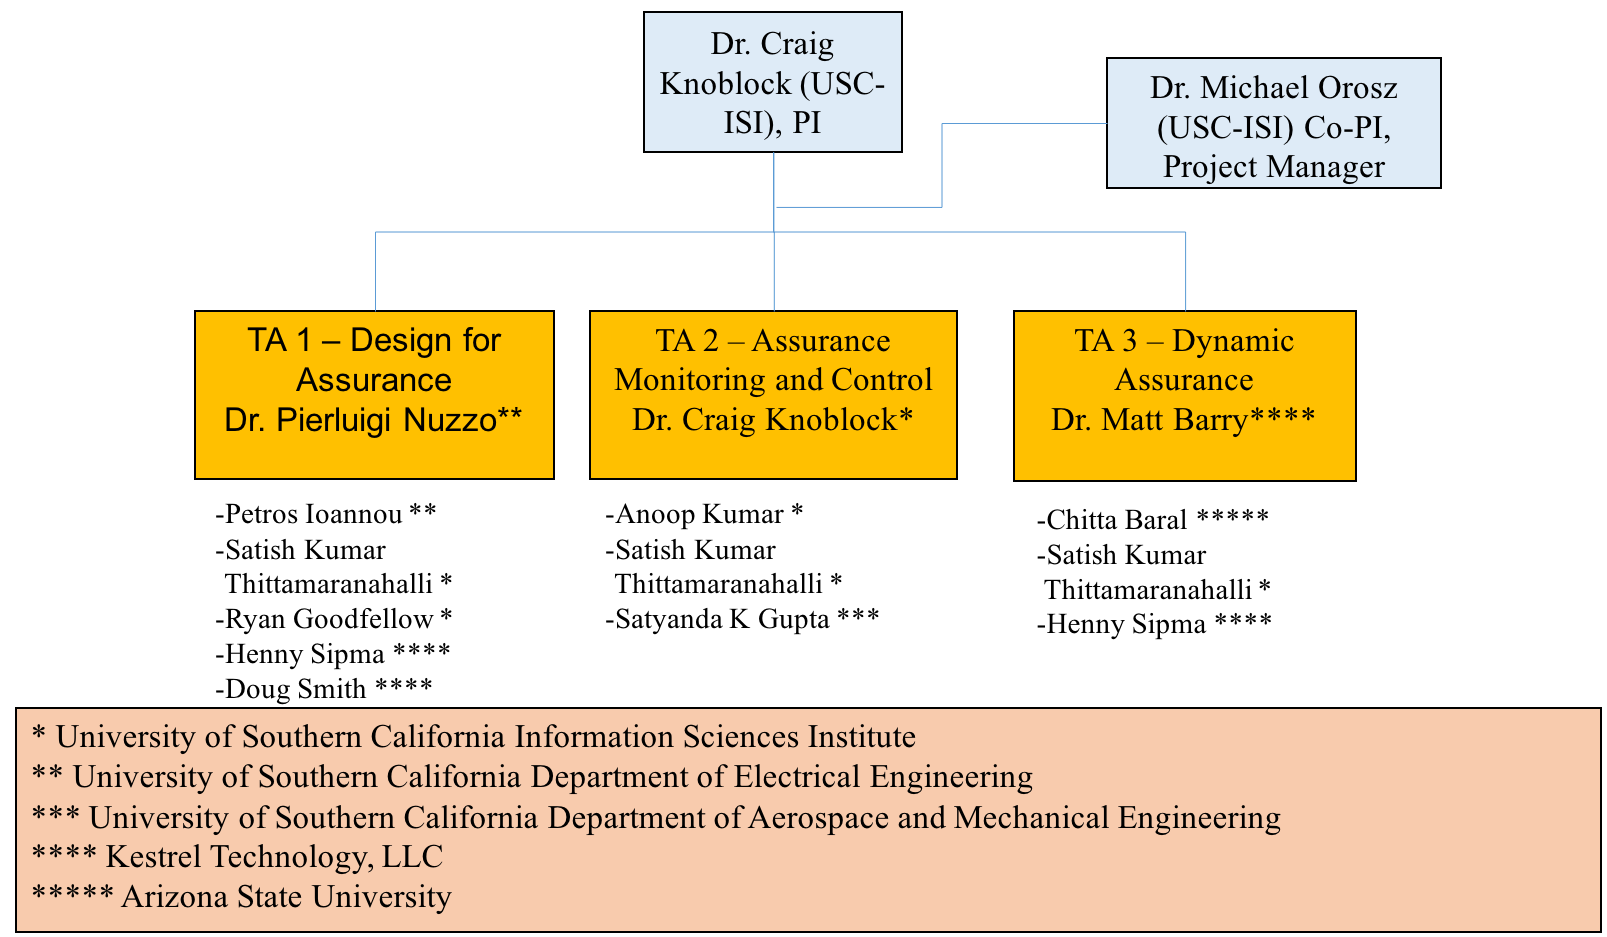
\includegraphics[width=6.0in]{./org-chart2.png}
\caption{\small Organization Chart}
\label{fig:org_chart}
\end{figure}

Coordination: To maximize collaboration and reduce risk to project failure from lack of communication and technical exchange, we plan to employ a wide variety of working styles and communication/coordination so that all can contribute.  At the core of our project will be regularly scheduled meetings bridging the diversely distributed team (Table~\ref{fig:Collaboration_Table}).  These meetings will address project status, identify challenges, implement risk mitigation strategies and participate in technology exchanges and system integration efforts (when appropriate)

\begin{table}[ht]
\caption{\small Project Meetings and Events}
  \centering
  {\footnotesize
\begin{tabular}{|m{3.15in}|m{3in}|} 
\hline
\textbf{Meeting} & \textbf{Frequency} 
\\\hline
Conference calls among investigators (discuss project status, address concerns and project risks) & Weekly
\\
\hline
Technical exchange and coordination meetings using Bluejeans or another videoconference technology & At least twice a month and more frequently as needed
  \\ 
\hline
Face-to-Face meetings (prior to P/I and demonstration meetings) & Every 3 to 6 months and more frequently (especially at the beginning of the project) as needed
 \\\cline{1-2}

\hline
\end{tabular}
}
\label{fig:Collaboration_Table}
\end{table}

\begin{table}[tbhp]
\caption{\small Key Project Team Member Responsibilities}
  \centering
  {\footnotesize
\begin{tabular}{| m{.75in} | m{3.9in}| m{1.5in}|} 
\hline
\textbf{Key Member} & \textbf{Responsibilities} & \textbf{Tasks} 
\\\hline
Dr.\ Craig Knoblock  & Principal Investigator responsible for project, leads TA 2 – Assurance Monitoring and Control.  Will lead the overall project and lead the TA2 team.  Served as the PI on many DARPA projects and has sucessfully led many large teams.    Effort on project:  25\% &
1.1.6, 1.2.2 1.2.3, 1.2.4, 1.3.4, 1.4.1, 
2.1.6, 2.2.2 2.2.3, 2.2.4, 2.3.4, 2.4.1, 
3.1.6, 3.2.2, 3.2.3, 3.2.4, 3.3.4, 3.4.1
\\
\hline
Dr.\ Michael Orosz & Co-Principal Investigator responsible managing the day-to-day operations of the project, assist technical teams as needed, coordinate with TA4 teams.    Has led many large complex multi-disciplined/multi-organizational projects in academic and industry environments.  Effort on project: 50\%
& 1.1.6, 2.1.6, 3.1.6, 1.4.1, 2.4.1, 3.4.1
  \\ 
\hline
Dr.\ Pierluigi Nuzzo 
& 
Co-Principal Investigator.  Leads the TA 1 - Design for Assurance team and conducts research on the formal methods for the design of the TA1 system.  Research experience on methodologies and tools for the design of cyber-physical systems; contracts, interfaces, and compositional methods for embedded system design; the application of automated formal methods and optimization theory to problems in embedded and cyber-physical systems.  Effort on project: 2 months/year (16.6\%)
& 
1.1.1, 2.1.1, 3.1.1 \\
\hline
Dr.\ Matthew Barry
& 
Key personnel.  Leads the TA 3 – Dynamic Assurance.   He will conduct the research on the dynamic assurance case language editors and parsers, the run-time system, and system integrations. Effort on project:  66\%
& 
1.3.2, 2.3.2, 3.3.2\\
\hline
Dr.\ Chitta Baral
& 
Key personnel responsible for learning assurance rules, supporting assurance rules with uncertainty and improving solver speed.  Expertise on ASP solvers, which will be used to reason about the assurance cases. Effort on project: 20\%
& 
1.3.1, 2.3.1, 3.3.1 \\
\hline
Dr.\ Doug Smith 
& 
Key personnel will support formal methods aspects of TA1, and lead the effort on abstract refinement. Expertise in field of automated correct-by-construction program generation.    Effort on project: 40\%
& 
1.1.5, 2.1.5, 3.1.5 \\
\hline
Dr.\ Henny Sipma
& 
Key personnel who will support the program verification tasks under TA1.  Will lead the effort on program verification.   Effort on project:  45\%
& 
1.1.5, 2.1.5, 3.1.5, 1.3.2, 2.3.2, 3.3.2 \\
\hline
Dr.\ Petros Ioannou
& 
Key personnel responsible providing and extending the assurance test bed, which will be available at the start of the project for autonomous vehicles.   Effort on project: 1 month/year (8.3\%)
& 
1.1.2, 2.1.2 (optional), 3.1.2 (optional)
\\
\hline
Dr.\ Satyandra Kumar Gupta
& 
Key Personnel providing autonomous command and control expertise to the TA-2 team.   Will lead the research on safety aware learning on TA2.   Past research on physics-aware decision making to facilitate automation.  Effort on project: 1 month/year (8.3\%)
& 
1.2.1, 2.2.1, 3.2.1 \\
\hline
Dr.\ Anoop Kumar 
& 
Key personnel providing support to the TA 2 project team.  Will lead the research on monitoring \& control and detecting distribution shifts.  Effort on project: 50\%
& 
1.2.1, 1.2.2, 1.2.3, 1.2.4, 2.2.1, 2.2.2, 2.2.3, 2.2.4, 3.2.1, 3.2.2, 3.2.3, 3.2.4\\
\hline
Dr.\ Satish Thittamaranahalli
& 
Key personnel developing scalable algorithms for TA1, TA2, and TA3 project teams.  Has extensive experience on scalable algorithm design, machine learning, and constraint reasoning.  Effort on project: 50\%
& 
1.2.1, 1.2.2, 1.2.3, 1.2.4, 2.2.1, 2.2.2, 2.2.3, 2.2.4, 3.2.1, 3.2.2, 3.2.3, 3.2.4, 1.1.4, 2.1.4, 3.1.4 \\
\hline
Dr.\ Ryan Goodfellow
& 
Key personnel providing support to the TA-1 project. Will lead the research on simulation-based testing.  Has extensive experience on simulation-based testing.  Effort on project:  30\%
& 
1.1.3, 2.1.3, 3.1.3 \\

\cline{1-2}

\hline
\end{tabular}
}
\label{fig:Table_Mgmt}
\end{table}



\newpage
\section{Personnel, Qualifications and Commitment}

{\bf Dr.\ Craig Knoblock}, the PI on this effort, is a Research Professor of both Computer Science and Spatial Sciences at the University of Southern California (USC) and Director of the Intelligent Systems Division at the USC Information Sciences Institute.   He received his Ph.D. from Carnegie Mellon University in computer science. 
%His research focuses on techniques for describing, acquiring, and exploiting the semantics of data.  
In previous projects he has worked on developing  scalable approaches to execution monitoring, accurate detection of sensor failures, and   automatic modeling and reconstruction of sensors.  He has published more than 300 journal articles, book chapters, and conference papers on these topics.  Dr. Knoblock is a Fellow of the Association for the Advancement of Artificial Intelligence (AAAI), a Distinguished Scientist of the Association of Computing Machinery (ACM), a Senior Member of IEEE, past President and Trustee of the International Joint Conference on Artificial Intelligence.
%and winner of the 2014 Robert S. Engelmore Award.  

{\bf Dr.\ Michael Orosz}, a Co-PI on this effort, is a Research Associate Professor of Civil and Environmental Engineering at the University of Southern California (USC) and Research Director of the Decision Systems Group at the USC Information Sciences Institute.  Dr. Orosz has over 30 years’ experience in commercial and government software development, basic and applied research, project management, academic research and has developed and deployed several commercially successful products.  His research interests are in machine learning and decision analytics as applied to intelligence analysis and autonomous command and control such as smart building controls.    Dr. Orosz has extensive experience in managing large complex multi-disciplined/multi-teamed research projects. %funded by DARPA, DHS, DoD, DoE, Industry, NASA, NRO, NSA and ONR.   
He received his Ph.D. in computer science from the University of California, Los Angeles.

{\bf Dr.\ Pierluigi Nuzzo}, a Co-PI on this project, is an Assistant Professor in the Department of Electrical Engineering at the University of Southern California. He received the Ph.D. in Electrical Engineering and Computer Sciences from the University of California at Berkeley. 
%in 2015, and the Laurea degree (MS) in electrical engineering (summa cum laude) from the University of Pisa, Italy, and the Sant'Anna School of Advanced Studies, Pisa, Italy.
%
%He has four years of research experience in analog and mixed signal circuit design as a researcher at IMEC, Leuven, Belgium, and over 10 years experience in design methodologies and tools for mixed-signal integrated circuits and cyber-physical systems, as a researcher at the University of Pisa, IMEC, UC Berkeley, and USC. 
His research interests
include: methodologies and tools for cyber-physical system and mixed-signal
system design; contracts, interfaces and compositional methods for embedded
system design; the application of formal methods and optimization theory to problems in embedded and cyber-physical systems and electronic design automation. 
%
Prof. Nuzzo received %First Place in the operational category and Best Overall
%Submission in the 2006 DAC/ISSCC Design Competition, 
a Marie Curie Fellowship
from the European Union in 2006, 
the University of California at Berkeley EECS
departmental fellowship in 2008, 
%the University of California at Berkeley Outstanding Graduate Student Instructor Award in 2013, 
the IBM Ph.D.
Fellowship in 2012 and 2014, 
%the Best Paper Award from the International Conference on Cyber-Physical Systems (ICCPS) in 2016, 
and the David J.~Sakrison Memorial Prize in 2016 for his doctoral research. 
%He is an author of 1 patent and over 60 publications.

{\bf Dr.\ Satyandra K. Gupta} is Smith International Professor in the Department of Aerospace and Mechanical Engineering at the University of Southern California. %Prior to joining the University of Southern California, he was a Professor in the Department of Mechanical Engineering and the Institute for Systems Research at the University of Maryland. He was the founding director of the Maryland Robotics Center and the Advanced Manufacturing Laboratory at the University of Maryland. 
He served as a program director for the National Robotics Initiative at the National Science Foundation from September 2012 to September 2014.  Dr. Gupta's interest is in the area of physics-aware decision making to facilitate automation. He has published more than 300 technical articles. He is a fellow of the American Society of Mechanical Engineers (ASME) and editor of ASME Journal of Computing and Information Science in Engineering. Dr. Gupta has received the Young Investigator Award from the Office of Naval Research in 2000, CAREER Award from the National Science Foundation in 2001, Presidential Early Career Award for Scientists and Engineers (PECASE) in 2001, Invention of the Year Award at the University of Maryland in 2007, Kos Ishii-Toshiba Award from ASME in 2011, and Excellence in Research Award from ASME in 2013.%, and Distinguished Alumnus Award from Indian Institute of Technology, Roorkee in 2014. %He has also received seven best paper awards at conferences.

{\bf Ryan Goodfellow} is a computer scientist at ISI working in combined cyber physical simulation and emulation platform development. His formal background is in simulation algorithms and modeling techniques using differential-algebraic equations (DAE). He has applied this knowledge in the CPS space by integrating DAE modeling languages and simulation engines with network testbeds to create comprehensive scientific experimentation platforms for cyber-physical systems. These experimentation platforms have been used in the power grid research space. %Ryan is a lead developer on the Deter network testbed, with a strong background in networked and distributed systems engineering. %He is also a combat veteran, serving as a non-commissioned officer and SIGINT team lead for a multi-functional intelligence team in Afghanistan.

{\bf Dr.\ Petros Ioannou} is a Professor in the Department of Electrical Engineering, Director of the Center for Advanced Transportation Technologies and Associate Director for Research for the DOT supported University Transportation Center at USC. He received his MS and PhD from the University of Illinois at Urbana Champaign in Mechanical and Electrical Engineering, respectively. His research interests are in robust adaptive control, vehicle dynamics and control, human factors and safety, automated vehicles, nonlinear systems and Intelligent transportation Systems.  He received the 2016 IEEE Transportation Technologies field award and the 2016 IEEE Control system society Transition to Practice Award. He is a Fellow of IEEE, IFAC and IET and author/coauthor of 8 books and over 400 papers.

{\bf Dr.\ Matthew Barry} will serve as lead for the TA3 tasks. %He will implement the dynamic assurance case language editors and parsers, the run-time system, and system integrations.  He will implement the assurance case arguments and the API for updating argument structure and content.  
Dr. Barry currently is CEO at Kestrel Technology LLC, and previously spent 20 years in NASA space mission operations at the Jet Propulsion Lab and Johnson Space Center.  At NASA Headquarters he led the introduction of dependability case requirements and plans for flight computing systems in upcoming manned space exploration missions, as well as the development of Agency-level software-related safety-critical control system requirements.  He recently served as a Principal Investigator on DHS/Cyber S\&T STAMP (Static Tool Analysis Modernization Program), DARPA CSFV (Crowd Sourced Formal Verification), three NASA Aeronautics R\&D projects, and the AFRL-sponsored Static Analysis of Numerical Algorithms project.  Dr. Barry earned BSME, MS, and PhD degrees in mechanical engineering, and an MBA degree, from Rice University.  

{\bf Dr.\ Henny Sipma} will support the program verification tasks under TA1.  %She is the key person behind the company's {\em KT Advance\/} and {\em KT Transferal\/} static analysis products, and the designer and programmer of the company's core {\em CodeHawk\/} abstract interpretation engine. 
Dr. Sipma currently is the CTO at Kestrel Technology LLC.  She has spent the past 10 years with Kestrel Technology as a static analysis expert; previously developed and taught static analysis techniques as senior research associate at Stanford University for eight years; and developed industrial process controls as an senior systems analyst at Shell.  She has been Principal Investigator or company lead on several recent R\&D projects for Federal agencies, including two projects under the IARPA STONESOUP (Securely Taking On New Executable Software of Uncertain Provenance) program; the DHS Cyber S\&T Gold Standard project; and the DARPA-sponsored STAC (Space-Time Analysis for Cybersecurity) and MUSE (Mining and Understanding Software Enclaves) programs.  Dr. Sipma earned 
%a BS degree in chemistry and an MS degree in chemical engineering at the University of Groningen in The Netherlands, and 
MS and PhD degrees in computer science from Stanford University.  

{\bf Dr.\ Douglas R.\ Smith} will support formal methods aspects of TA1, including the enforcement of safety properties and the generation of monitors.  He is President of Kestrel Technology LLC and Principal Scientist at Kestrel Institute.  He is a Fellow of the American Association of Artificial Intelligence (AAAI) and an ASE Fellow (Automated Software Engineering).  From 1986 to 2000, he taught an advanced graduate course on correct-by-construction software development at Stanford.  
%Dr. Smith has led the development of a series of software synthesis systems, including KIDS (Kestrel Interactive Development System), Specware, Designware, and Planware. 
%Applications domains have included a variety of complex high-performance planners and schedulers for the US Air Force.  He leads current projects on the generation of air mission plans and cyberoperations.  
Other recent projects focused on automated policy enforcement \cite{SmithD0703,SmithD08}, synthesis of secure network protocol codes, and the synthesis of high-performance constraint-solvers\cite{SmithD08c,SmithD13}.  Dr. Smith has over 30 years experience in the field of automated correct-by-construction program generation and has published over 100 papers. He has one patent.  He received the Ph.D. in Computer Science from Duke University% in 1979.  

{\bf Dr. Chitta Baral} is a Professor in the Department of Computer Science and Engineering at Arizona State University. He will support the TA3 efforts on Learning assurance rules, supporting assurance rules with uncertainty and improving solver speed. Dr. Baral has expertise in various aspects of autonomy and Artificial Intelligence. 
He wrote the first book on answer set programming (published by Cambridge University Press) the formal language behind our assurance rules. Some of his other works relevant to this proposal are: goal specification for autonomous systems, automatic construction of control rules for autonomous systems that satisfy given goals, combining machine learning with reasoning in various contexts, including image understanding. %He is the President of KR Inc. He is an associate editor of AIJ and has been an associate editor of JAIR.

{\bf Dr.\ Satish Kumar Thittamaranahalli (T. K. Satish Kumar)} leads the Collaboratory for Algorithmic Techniques and Artificial Intelligence (CATAI) at USC's Information Sciences Institute. He has published over 60 papers on numerous topics in Artificial Intelligence spanning such diverse areas as Constraint Reasoning, Planning and Scheduling, Probabilistic Reasoning, Robotics, Combinatorial Optimization, Approximation and Randomization, Heuristic Search, Model-Based Reasoning, Knowledge Representation and Spatio-Temporal Reasoning. %He %has served on the Program Committees of many international conferences in Artificial Intelligence
He and is a winner of the 2016 Best Robotics Paper Award and the 2005 Best Student Paper Award from the International Conference on Automated Planning and Scheduling. 
Dr. Kumar received his PhD in Computer Science from Stanford University. %In the past, he has also been a Visiting Student at the NASA Ames Research Center, a Postdoctoral Research Scholar at the University of California, Berkeley, a Research Scientist at the Institute for Human and Machine Cognition, a Visiting Assistant Professor at the University of West Florida, and a Senior Research and Development Scientist at Mission Critical Technologies.

\textbf{Dr.\ Anoop Kumar} is a senior computer scientist at USC ISI and has broad expertise in machine learning, statistical modeling, and software engineering.  Dr.\ Kumar is the technical lead on the DARPA RSPACE program and has played a vital role in developing a system that fuses air operations data from multiple sources, maintains world state, and issues warnings. Previously, he led the research and development of the BBN’s election forecasting system for the IARPA OSI program. %Dr.\ Kumar played a significant role in the DARPA DEFT program by developing a model to support integration of output from multiple NLP algorithms. He has contributed at the development to management levels on government research contracts and commercial projects. 
Dr.\ Kumar helped design and develop BBN's commercially available, hosted speech and medical transcription services offering. 

\begin{table}[!tbh]
\begin{footnotesize}
\vspace{-0.1in}

\begin{tabular}{lll}
\begin{tabular}[t]{|l|@{}c@{}|@{}c@{}|@{}c@{}|@{}c@{}|} \hline
Project & Status & \multicolumn{3}{ c| }{Hours} \\ \cline{3-5}
& & P1 & P2 & P3 \\ \hline



\multicolumn{5}{ |c| }{ \textbf{Craig Knoblock} } \\ \cline{1-5}
Safeguard & Pro & 770 & 641 & 641 \\ \cline{1-5}
ELICIT & Cur & 308 & 256 & 120 \\ \cline{1-5}
WTNIC & Cur & 11 & 0 & 0 \\ \cline{1-5}
EFFECT & Cur & 641 & 107 & 0 \\ \cline{1-5}
LinkedMaps & Cur & 203 & 25 & 0 \\ \cline{1-5}
PRINCESS & Cur & 608 & 96 & 0 \\ \cline{1-5}
SCHARP & Cur & 481 & 54 & 0 \\ \cline{1-5}
MINT & Pen & 650 & 534 & 285 \\ \cline{1-5}

\multicolumn{5}{ |c| }{ \textbf{Michael Orosz} } \\ \cline{1-5}
Safeguard & Pro & 1560 & 1300 & 1300  \\ \cline{1-5}
SMC/SY & Cur & 1803 & 0 & 0  \\ \cline{1-5}

\multicolumn{5}{ |c| }{ \textbf{Matthew Barry} } \\ \cline{1-5}
Safeguard & Pro & 2078 & 1690 & 1554 \\ \cline{1-5}
Starlite & Cur & 1840 & 1692 & 0 \\ \cline{1-5}



\multicolumn{5}{ |c| }{ \textbf{Anoop Kumar} } \\ \cline{1-5}
Safeguard & Pro & 1560 & 1300 & 1300 \\ \cline{1-5}

\end{tabular}
&
\begin{tabular}[t]{|l|@{}c@{}|@{}c@{}|@{}c@{}|@{}c@{}|} \hline
Project & Status & \multicolumn{3}{ c| }{Hours} \\ \cline{3-5}
& & P1 & P2 & P3 \\ \hline

\multicolumn{5}{ |c| }{ \textbf{Pierluigi Nuzzo} } \\ \cline{1-5}
Safeguard & Pro & 520 & 433 & 433  \\ \cline{1-5}
Mirage & Cur & 433 & 0 & 0  \\ \cline{1-5}

\multicolumn{5}{ |c| }{ \textbf{Satyandra Gupta} } \\ \cline{1-5}
Safeguard & Pro & 260 & 217 & 217 \\ \cline{1-5}
Human   & Cur & 22 & 0 & 0 \\ \cline{1-5}
Vehicles & Cur & 36 & 0 & 0 \\ \cline{1-5}
Robot & Cur & 116 & 0 & 0 \\ \cline{1-5}
Assembly & Cur & 33 & 0 & 0 \\ \cline{1-5}
Solar & Cur & 4 & 0 & 0 \\ \cline{1-5}

\multicolumn{5}{ |c| }{ \textbf{Petros Ioannou} } \\ \cline{1-5}
Safeguard & Pro & 260 & 217 & 217 \\ \cline{1-5}
CPS & Cur & 130 & 0 & 0 \\ \cline{1-5}

\multicolumn{5}{ |c| }{ \textbf{Ryan Goodfellow} } \\ \cline{1-5}
Safeguard & Pro & 936 & 780 & 780 \\ \cline{1-5}
STEAM & Cur & 416 & 0 & 0 \\ \cline{1-5}


\end{tabular}
&
\begin{tabular}[t]{|l|@{}c@{}|@{}c@{}|@{}c@{}|@{}c@{}|} \hline
Project & Status & \multicolumn{3}{ c| }{Hours} \\ \cline{3-5}
& & P1 & P2 & P3 \\ \hline

\multicolumn{5}{ |c| }{ \textbf{Chitta Baral} } \\ \cline{1-5}
Safeguard & Pro & 659 & 485 & 485 \\ \cline{1-5}
PostdocBP & Cur & 176 & 0 & 0 \\ \cline{1-5}
Languages & Pen & 528 & 264 & 264 \\ \cline{1-5}
CAREER & Pen & 88 & 44 & 44 \\ \cline{1-5}
CHS & Pen & 510 & 255 & 0 \\ \cline{1-5}

\multicolumn{5}{ |c| }{ \textbf{Doug Smith} } \\ \cline{1-5}
Safeguard & Pro & 1222 & 984 & 840 \\ \cline{1-5}
RSPACE & Cur & 342 & 0 & 0 \\ 
\cline{1-5}
PLANX & Cur & 154 & 0 & 0 \\ 
\cline{1-5}
HACCS & Pen & 923 & 769 & 769 \\ 
\cline{1-5}

\multicolumn{5}{ |c| }{ \textbf{Henny Sipma} } \\ \cline{1-5}
Safeguard & Pro & 1372 & 962 & 840 \\ \cline{1-5}
STAC & Cur & 797 & 0 & 0 \\ \cline{1-5}

\multicolumn{5}{ |c| }{ \textbf{Satish Thittamaranahalli} } \\ \cline{1-5}
Safeguard & Pro & 1560 & 1300 & 1300 \\ \cline{1-5}
MapF & Cur & 103 & 103 & 0 \\ \cline{1-5}

\end{tabular}
\end{tabular}

\end{footnotesize}
\caption{Individual commitments of key personnel}
\label{tab:Commitments}
\vspace{-0.2in}
\end{table}

\clearpage
\newpage
\section{Capabilities}


%\subsection{University of Southern California}
USC has strengths in number of areas that are closely related to the proposed work:
\begin{itemize}[itemsep=0pt,leftmargin=*]
\item Dr.\ Nuzzo 
%has over 10-year research experience in embedded system design, from mixed-signal chip design (analog-to-digital converters, frequency synthesizers, software-defined radio), to methodologies and tools for mixed-signal integrated circuits and Cyber-Physical Systems (CPSs), and the application of formal methods and optimization theory to problems in embedded and cyber-physical systems and electronic design automation.  
%His doctoral work 
has done extensive research on contracts and compositional methods for heterogeneous system design and design space exploration, with application to aircraft electric power systems and environmental control systems. His work has helped transition rigorous system design foundations, innovative design methodologies, and new systems engineering paradigms to industry (IBM, United Technologies). 
\item Dr.\ Satyandra K. Gupta has worked on autonomous surface vehicles, autonomous ground vehicles for operation on rugged terrains, and autonomous flapping wing aerial vehicles.   His group has developed a hierarchal decision making approach for realizing autonomous systems. 
%This approach combines task planning and assignment, deliberative trajectory planning, reactive collision avoidance behaviors, and trajectory tracking control layers. 
His group has also developed new methods for learning reactive behaviors in adversarial environments and COLREGS compliant trajectory planning. \item Dr.\ Knoblock has developed methods that learn the relationships between sensors to both identify failures and changes in sensor and reconstruct those sensors, providing estimates of the accuracy of the reconstructed sensors.  
\item Ryan Goodfellow has extensive experience in simulation based testing through high-fidelity CPS testbed environment development and operation, using the Deter network testbed as the core which has supported several large scale government projects from a variety of agencies and thousands of users. %we have developed sophisticated CPS experiments under programs such as NFS RIPS, NIST SmartCities and the DHS Cybersecurity showcase.
\item Dr.\ Ioannou %helped  design and implement adaptive cruise control systems in collaboration with Ford Motor Company, which was commercialized four years before any other company. He 
worked on several DOT funded projects on automated vehicles and intelligent highway systems where he demonstrated his vehicle control designs for safety and performance on actual automated vehicles in test trucks and I-15 highway.
\item Drs.\ Knoblock, Kumar, and Thittamaranahalli have developed highly scalable approaches for monitoring message traffic to identify potential problems and issue warnings and alerts. 
\item Dr. Thittamaranahalli has developed state-of-the-art methods for efficiently solving large-scale search and optimization problems. %These techniques will be applicable in TA2 for safety-aware learning and planning, in TA2 for assurance monitoring and control, and in TA3 for dynamic assessment of assurance cases.

\end{itemize}
%\subsection{Kestrel Technology LLC}

Kestrel Technology's strength is in program analysis, specifically static analysis of both source and binary targets.  The company performs applied R\&D and product development for a variety of static analysis applications  pivoting primarily on the abstract interpretation technique.  The company recently initiated development of program analysis applications using logical equivalence techniques. As a provider of verification evidence in the form of mathematical proofs, the company also has expertise in the design and development of assurance case arguments for high-integrity systems using such evidence. %The company is engaged in a partnership with Wind River Systems to develop program analysis tools for its embedded system developers.  Many of Wind River's customers must develop their products under safety and certification standards, including those using safety cases.  

   

%\subsection{Arizona State University}
Chitta Baral at Arizona State University has developed various software to learn assurance rules and various ASP solvers, which he has made available as open-source.

Most of the software carried forward for implementation or derivation is open source.  The single exception is Kestrel Technology's {\it KT Advance\/} static analysis tool (TA1), in particular the abstract interpretation engine therein, which is company proprietary and is US EAR export-controlled.   
%Owing to mixed funding for the development of that technology 
We will continue to provide the Federal government a restricted use license for that particular item.

There are no specialized facilities, data, or GFE required for this effort. 

\include{sow}
\include{milestones}

% \section{Level of Effort by Task \textcolor{red}{[Mike/Lisa - 1 pages]}}

% \textcolor{blue}{
% \begin{itemize}
% \item Will be a separate spreadsheet
% \item
% \end{itemize}
% }

\include{appendix_a}

%\section{Appendix B \textcolor{red}{[No Page Count]}}

\section{References}
\bibliographystyle{acm} 
\bibliography{TA3/ta3,TA2/ta2,TA1/ta1}
\end{document}
\clearpage
\newpage


\section{Management Plan}


The Principal Investigator for this effort is Dr. Craig Knoblock who is responsible for all aspects of the effort, will coordinate the parallel team efforts, and will ensure high levels of performance from individual team members.  The Co-P/I, Dr. Michael Orosz, will provide project management and will assist all performers in the execution of the project.    The project team is divided into three working groups (Figure~\ref{fig:org_chart}) corresponding to Technical Areas 1-3, however, members of each team contribute across all project activities.   Table~\ref{fig:Table_Mgmt} defines the major contributions of each project team member to the project tasks.

\begin{figure}[tbhp]
%\vspace{-25pt}
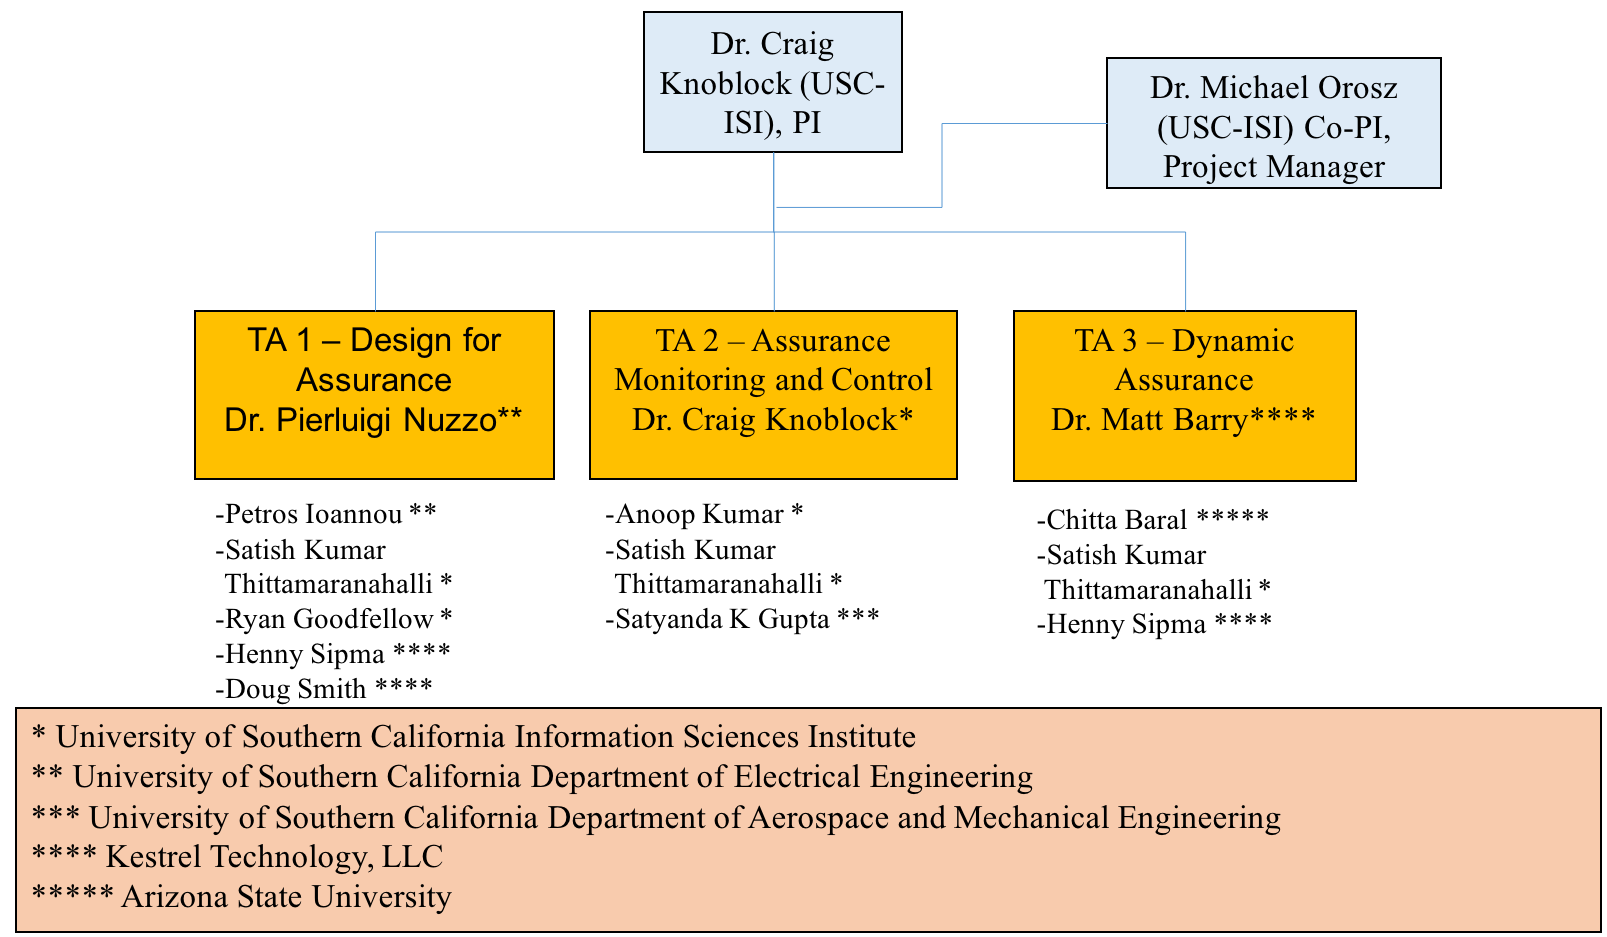
\includegraphics[width=6.0in]{./org-chart2.png}
\caption{\small Organization Chart}
\label{fig:org_chart}
\end{figure}

Coordination: To maximize collaboration and reduce risk to project failure from lack of communication and technical exchange, we plan to employ a wide variety of working styles and communication/coordination so that all can contribute.  At the core of our project will be regularly scheduled meetings bridging the diversely distributed team (Table~\ref{fig:Collaboration_Table}).  These meetings will address project status, identify challenges, implement risk mitigation strategies and participate in technology exchanges and system integration efforts (when appropriate)

\begin{table}[ht]
\caption{\small Project Meetings and Events}
  \centering
  {\footnotesize
\begin{tabular}{|m{3.15in}|m{3in}|} 
\hline
\textbf{Meeting} & \textbf{Frequency} 
\\\hline
Conference calls among investigators (discuss project status, address concerns and project risks) & Weekly
\\
\hline
Technical exchange and coordination meetings using Bluejeans or another videoconference technology & At least twice a month and more frequently as needed
  \\ 
\hline
Face-to-Face meetings (prior to P/I and demonstration meetings) & Every 3 to 6 months and more frequently (especially at the beginning of the project) as needed
 \\\cline{1-2}

\hline
\end{tabular}
}
\label{fig:Collaboration_Table}
\end{table}

\begin{table}[tbhp]
\caption{\small Key Project Team Member Responsibilities}
  \centering
  {\footnotesize
\begin{tabular}{| m{.75in} | m{3.9in}| m{1.5in}|} 
\hline
\textbf{Key Member} & \textbf{Responsibilities} & \textbf{Tasks} 
\\\hline
Dr.\ Craig Knoblock  & Principal Investigator responsible for project, leads TA 2 – Assurance Monitoring and Control.  Will lead the overall project and lead the TA2 team.  Served as the PI on many DARPA projects and has sucessfully led many large teams.    Effort on project:  25\% &
1.1.6, 1.2.2 1.2.3, 1.2.4, 1.3.4, 1.4.1, 
2.1.6, 2.2.2 2.2.3, 2.2.4, 2.3.4, 2.4.1, 
3.1.6, 3.2.2, 3.2.3, 3.2.4, 3.3.4, 3.4.1
\\
\hline
Dr.\ Michael Orosz & Co-Principal Investigator responsible managing the day-to-day operations of the project, assist technical teams as needed, coordinate with TA4 teams.    Has led many large complex multi-disciplined/multi-organizational projects in academic and industry environments.  Effort on project: 50\%
& 1.1.6, 2.1.6, 3.1.6, 1.4.1, 2.4.1, 3.4.1
  \\ 
\hline
Dr.\ Pierluigi Nuzzo 
& 
Co-Principal Investigator.  Leads the TA 1 - Design for Assurance team and conducts research on the formal methods for the design of the TA1 system.  Research experience on methodologies and tools for the design of cyber-physical systems; contracts, interfaces, and compositional methods for embedded system design; the application of automated formal methods and optimization theory to problems in embedded and cyber-physical systems.  Effort on project: 2 months/year (16.6\%)
& 
1.1.1, 2.1.1, 3.1.1 \\
\hline
Dr.\ Matthew Barry
& 
Key personnel.  Leads the TA 3 – Dynamic Assurance.   He will conduct the research on the dynamic assurance case language editors and parsers, the run-time system, and system integrations. Effort on project:  66\%
& 
1.3.2, 2.3.2, 3.3.2\\
\hline
Dr.\ Chitta Baral
& 
Key personnel responsible for learning assurance rules, supporting assurance rules with uncertainty and improving solver speed.  Expertise on ASP solvers, which will be used to reason about the assurance cases. Effort on project: 20\%
& 
1.3.1, 2.3.1, 3.3.1 \\
\hline
Dr.\ Doug Smith 
& 
Key personnel will support formal methods aspects of TA1, and lead the effort on abstract refinement. Expertise in field of automated correct-by-construction program generation.    Effort on project: 40\%
& 
1.1.5, 2.1.5, 3.1.5 \\
\hline
Dr.\ Henny Sipma
& 
Key personnel who will support the program verification tasks under TA1.  Will lead the effort on program verification.   Effort on project:  45\%
& 
1.1.5, 2.1.5, 3.1.5, 1.3.2, 2.3.2, 3.3.2 \\
\hline
Dr.\ Petros Ioannou
& 
Key personnel responsible providing and extending the assurance test bed, which will be available at the start of the project for autonomous vehicles.   Effort on project: 1 month/year (8.3\%)
& 
1.1.2, 2.1.2 (optional), 3.1.2 (optional)
\\
\hline
Dr.\ Satyandra Kumar Gupta
& 
Key Personnel providing autonomous command and control expertise to the TA-2 team.   Will lead the research on safety aware learning on TA2.   Past research on physics-aware decision making to facilitate automation.  Effort on project: 1 month/year (8.3\%)
& 
1.2.1, 2.2.1, 3.2.1 \\
\hline
Dr.\ Anoop Kumar 
& 
Key personnel providing support to the TA 2 project team.  Will lead the research on monitoring \& control and detecting distribution shifts.  Effort on project: 50\%
& 
1.2.1, 1.2.2, 1.2.3, 1.2.4, 2.2.1, 2.2.2, 2.2.3, 2.2.4, 3.2.1, 3.2.2, 3.2.3, 3.2.4\\
\hline
Dr.\ Satish Thittamaranahalli
& 
Key personnel developing scalable algorithms for TA1, TA2, and TA3 project teams.  Has extensive experience on scalable algorithm design, machine learning, and constraint reasoning.  Effort on project: 50\%
& 
1.2.1, 1.2.2, 1.2.3, 1.2.4, 2.2.1, 2.2.2, 2.2.3, 2.2.4, 3.2.1, 3.2.2, 3.2.3, 3.2.4, 1.1.4, 2.1.4, 3.1.4 \\
\hline
Dr.\ Ryan Goodfellow
& 
Key personnel providing support to the TA-1 project. Will lead the research on simulation-based testing.  Has extensive experience on simulation-based testing.  Effort on project:  30\%
& 
1.1.3, 2.1.3, 3.1.3 \\

\cline{1-2}

\hline
\end{tabular}
}
\label{fig:Table_Mgmt}
\end{table}



\newpage
\section{Personnel, Qualifications and Commitment}

{\bf Dr.\ Craig Knoblock}, the PI on this effort, is a Research Professor of both Computer Science and Spatial Sciences at the University of Southern California (USC) and Director of the Intelligent Systems Division at the USC Information Sciences Institute.   He received his Ph.D. from Carnegie Mellon University in computer science. 
%His research focuses on techniques for describing, acquiring, and exploiting the semantics of data.  
In previous projects he has worked on developing  scalable approaches to execution monitoring, accurate detection of sensor failures, and   automatic modeling and reconstruction of sensors.  He has published more than 300 journal articles, book chapters, and conference papers on these topics.  Dr. Knoblock is a Fellow of the Association for the Advancement of Artificial Intelligence (AAAI), a Distinguished Scientist of the Association of Computing Machinery (ACM), a Senior Member of IEEE, past President and Trustee of the International Joint Conference on Artificial Intelligence.
%and winner of the 2014 Robert S. Engelmore Award.  

{\bf Dr.\ Michael Orosz}, a Co-PI on this effort, is a Research Associate Professor of Civil and Environmental Engineering at the University of Southern California (USC) and Research Director of the Decision Systems Group at the USC Information Sciences Institute.  Dr. Orosz has over 30 years’ experience in commercial and government software development, basic and applied research, project management, academic research and has developed and deployed several commercially successful products.  His research interests are in machine learning and decision analytics as applied to intelligence analysis and autonomous command and control such as smart building controls.    Dr. Orosz has extensive experience in managing large complex multi-disciplined/multi-teamed research projects. %funded by DARPA, DHS, DoD, DoE, Industry, NASA, NRO, NSA and ONR.   
He received his Ph.D. in computer science from the University of California, Los Angeles.

{\bf Dr.\ Pierluigi Nuzzo}, a Co-PI on this project, is an Assistant Professor in the Department of Electrical Engineering at the University of Southern California. He received the Ph.D. in Electrical Engineering and Computer Sciences from the University of California at Berkeley. 
%in 2015, and the Laurea degree (MS) in electrical engineering (summa cum laude) from the University of Pisa, Italy, and the Sant'Anna School of Advanced Studies, Pisa, Italy.
%
%He has four years of research experience in analog and mixed signal circuit design as a researcher at IMEC, Leuven, Belgium, and over 10 years experience in design methodologies and tools for mixed-signal integrated circuits and cyber-physical systems, as a researcher at the University of Pisa, IMEC, UC Berkeley, and USC. 
His research interests
include: methodologies and tools for cyber-physical system and mixed-signal
system design; contracts, interfaces and compositional methods for embedded
system design; the application of formal methods and optimization theory to problems in embedded and cyber-physical systems and electronic design automation. 
%
Prof. Nuzzo received %First Place in the operational category and Best Overall
%Submission in the 2006 DAC/ISSCC Design Competition, 
a Marie Curie Fellowship
from the European Union in 2006, 
the University of California at Berkeley EECS
departmental fellowship in 2008, 
%the University of California at Berkeley Outstanding Graduate Student Instructor Award in 2013, 
the IBM Ph.D.
Fellowship in 2012 and 2014, 
%the Best Paper Award from the International Conference on Cyber-Physical Systems (ICCPS) in 2016, 
and the David J.~Sakrison Memorial Prize in 2016 for his doctoral research. 
%He is an author of 1 patent and over 60 publications.

{\bf Dr.\ Satyandra K. Gupta} is Smith International Professor in the Department of Aerospace and Mechanical Engineering at the University of Southern California. %Prior to joining the University of Southern California, he was a Professor in the Department of Mechanical Engineering and the Institute for Systems Research at the University of Maryland. He was the founding director of the Maryland Robotics Center and the Advanced Manufacturing Laboratory at the University of Maryland. 
He served as a program director for the National Robotics Initiative at the National Science Foundation from September 2012 to September 2014.  Dr. Gupta's interest is in the area of physics-aware decision making to facilitate automation. He has published more than 300 technical articles. He is a fellow of the American Society of Mechanical Engineers (ASME) and editor of ASME Journal of Computing and Information Science in Engineering. Dr. Gupta has received the Young Investigator Award from the Office of Naval Research in 2000, CAREER Award from the National Science Foundation in 2001, Presidential Early Career Award for Scientists and Engineers (PECASE) in 2001, Invention of the Year Award at the University of Maryland in 2007, Kos Ishii-Toshiba Award from ASME in 2011, and Excellence in Research Award from ASME in 2013.%, and Distinguished Alumnus Award from Indian Institute of Technology, Roorkee in 2014. %He has also received seven best paper awards at conferences.

{\bf Ryan Goodfellow} is a computer scientist at ISI working in combined cyber physical simulation and emulation platform development. His formal background is in simulation algorithms and modeling techniques using differential-algebraic equations (DAE). He has applied this knowledge in the CPS space by integrating DAE modeling languages and simulation engines with network testbeds to create comprehensive scientific experimentation platforms for cyber-physical systems. These experimentation platforms have been used in the power grid research space. %Ryan is a lead developer on the Deter network testbed, with a strong background in networked and distributed systems engineering. %He is also a combat veteran, serving as a non-commissioned officer and SIGINT team lead for a multi-functional intelligence team in Afghanistan.

{\bf Dr.\ Petros Ioannou} is a Professor in the Department of Electrical Engineering, Director of the Center for Advanced Transportation Technologies and Associate Director for Research for the DOT supported University Transportation Center at USC. He received his MS and PhD from the University of Illinois at Urbana Champaign in Mechanical and Electrical Engineering, respectively. His research interests are in robust adaptive control, vehicle dynamics and control, human factors and safety, automated vehicles, nonlinear systems and Intelligent transportation Systems.  He received the 2016 IEEE Transportation Technologies field award and the 2016 IEEE Control system society Transition to Practice Award. He is a Fellow of IEEE, IFAC and IET and author/coauthor of 8 books and over 400 papers.

{\bf Dr.\ Matthew Barry} will serve as lead for the TA3 tasks. %He will implement the dynamic assurance case language editors and parsers, the run-time system, and system integrations.  He will implement the assurance case arguments and the API for updating argument structure and content.  
Dr. Barry currently is CEO at Kestrel Technology LLC, and previously spent 20 years in NASA space mission operations at the Jet Propulsion Lab and Johnson Space Center.  At NASA Headquarters he led the introduction of dependability case requirements and plans for flight computing systems in upcoming manned space exploration missions, as well as the development of Agency-level software-related safety-critical control system requirements.  He recently served as a Principal Investigator on DHS/Cyber S\&T STAMP (Static Tool Analysis Modernization Program), DARPA CSFV (Crowd Sourced Formal Verification), three NASA Aeronautics R\&D projects, and the AFRL-sponsored Static Analysis of Numerical Algorithms project.  Dr. Barry earned BSME, MS, and PhD degrees in mechanical engineering, and an MBA degree, from Rice University.  

{\bf Dr.\ Henny Sipma} will support the program verification tasks under TA1.  %She is the key person behind the company's {\em KT Advance\/} and {\em KT Transferal\/} static analysis products, and the designer and programmer of the company's core {\em CodeHawk\/} abstract interpretation engine. 
Dr. Sipma currently is the CTO at Kestrel Technology LLC.  She has spent the past 10 years with Kestrel Technology as a static analysis expert; previously developed and taught static analysis techniques as senior research associate at Stanford University for eight years; and developed industrial process controls as an senior systems analyst at Shell.  She has been Principal Investigator or company lead on several recent R\&D projects for Federal agencies, including two projects under the IARPA STONESOUP (Securely Taking On New Executable Software of Uncertain Provenance) program; the DHS Cyber S\&T Gold Standard project; and the DARPA-sponsored STAC (Space-Time Analysis for Cybersecurity) and MUSE (Mining and Understanding Software Enclaves) programs.  Dr. Sipma earned 
%a BS degree in chemistry and an MS degree in chemical engineering at the University of Groningen in The Netherlands, and 
MS and PhD degrees in computer science from Stanford University.  

{\bf Dr.\ Douglas R.\ Smith} will support formal methods aspects of TA1, including the enforcement of safety properties and the generation of monitors.  He is President of Kestrel Technology LLC and Principal Scientist at Kestrel Institute.  He is a Fellow of the American Association of Artificial Intelligence (AAAI) and an ASE Fellow (Automated Software Engineering).  From 1986 to 2000, he taught an advanced graduate course on correct-by-construction software development at Stanford.  
%Dr. Smith has led the development of a series of software synthesis systems, including KIDS (Kestrel Interactive Development System), Specware, Designware, and Planware. 
%Applications domains have included a variety of complex high-performance planners and schedulers for the US Air Force.  He leads current projects on the generation of air mission plans and cyberoperations.  
Other recent projects focused on automated policy enforcement \cite{SmithD0703,SmithD08}, synthesis of secure network protocol codes, and the synthesis of high-performance constraint-solvers\cite{SmithD08c,SmithD13}.  Dr. Smith has over 30 years experience in the field of automated correct-by-construction program generation and has published over 100 papers. He has one patent.  He received the Ph.D. in Computer Science from Duke University% in 1979.  

{\bf Dr. Chitta Baral} is a Professor in the Department of Computer Science and Engineering at Arizona State University. He will support the TA3 efforts on Learning assurance rules, supporting assurance rules with uncertainty and improving solver speed. Dr. Baral has expertise in various aspects of autonomy and Artificial Intelligence. 
He wrote the first book on answer set programming (published by Cambridge University Press) the formal language behind our assurance rules. Some of his other works relevant to this proposal are: goal specification for autonomous systems, automatic construction of control rules for autonomous systems that satisfy given goals, combining machine learning with reasoning in various contexts, including image understanding. %He is the President of KR Inc. He is an associate editor of AIJ and has been an associate editor of JAIR.

{\bf Dr.\ Satish Kumar Thittamaranahalli (T. K. Satish Kumar)} leads the Collaboratory for Algorithmic Techniques and Artificial Intelligence (CATAI) at USC's Information Sciences Institute. He has published over 60 papers on numerous topics in Artificial Intelligence spanning such diverse areas as Constraint Reasoning, Planning and Scheduling, Probabilistic Reasoning, Robotics, Combinatorial Optimization, Approximation and Randomization, Heuristic Search, Model-Based Reasoning, Knowledge Representation and Spatio-Temporal Reasoning. %He %has served on the Program Committees of many international conferences in Artificial Intelligence
He and is a winner of the 2016 Best Robotics Paper Award and the 2005 Best Student Paper Award from the International Conference on Automated Planning and Scheduling. 
Dr. Kumar received his PhD in Computer Science from Stanford University. %In the past, he has also been a Visiting Student at the NASA Ames Research Center, a Postdoctoral Research Scholar at the University of California, Berkeley, a Research Scientist at the Institute for Human and Machine Cognition, a Visiting Assistant Professor at the University of West Florida, and a Senior Research and Development Scientist at Mission Critical Technologies.

\textbf{Dr.\ Anoop Kumar} is a senior computer scientist at USC ISI and has broad expertise in machine learning, statistical modeling, and software engineering.  Dr.\ Kumar is the technical lead on the DARPA RSPACE program and has played a vital role in developing a system that fuses air operations data from multiple sources, maintains world state, and issues warnings. Previously, he led the research and development of the BBN’s election forecasting system for the IARPA OSI program. %Dr.\ Kumar played a significant role in the DARPA DEFT program by developing a model to support integration of output from multiple NLP algorithms. He has contributed at the development to management levels on government research contracts and commercial projects. 
Dr.\ Kumar helped design and develop BBN's commercially available, hosted speech and medical transcription services offering. 

\begin{table}[!tbh]
\begin{footnotesize}
\vspace{-0.1in}

\begin{tabular}{lll}
\begin{tabular}[t]{|l|@{}c@{}|@{}c@{}|@{}c@{}|@{}c@{}|} \hline
Project & Status & \multicolumn{3}{ c| }{Hours} \\ \cline{3-5}
& & P1 & P2 & P3 \\ \hline



\multicolumn{5}{ |c| }{ \textbf{Craig Knoblock} } \\ \cline{1-5}
Safeguard & Pro & 770 & 641 & 641 \\ \cline{1-5}
ELICIT & Cur & 308 & 256 & 120 \\ \cline{1-5}
WTNIC & Cur & 11 & 0 & 0 \\ \cline{1-5}
EFFECT & Cur & 641 & 107 & 0 \\ \cline{1-5}
LinkedMaps & Cur & 203 & 25 & 0 \\ \cline{1-5}
PRINCESS & Cur & 608 & 96 & 0 \\ \cline{1-5}
SCHARP & Cur & 481 & 54 & 0 \\ \cline{1-5}
MINT & Pen & 650 & 534 & 285 \\ \cline{1-5}

\multicolumn{5}{ |c| }{ \textbf{Michael Orosz} } \\ \cline{1-5}
Safeguard & Pro & 1560 & 1300 & 1300  \\ \cline{1-5}
SMC/SY & Cur & 1803 & 0 & 0  \\ \cline{1-5}

\multicolumn{5}{ |c| }{ \textbf{Matthew Barry} } \\ \cline{1-5}
Safeguard & Pro & 2078 & 1690 & 1554 \\ \cline{1-5}
Starlite & Cur & 1840 & 1692 & 0 \\ \cline{1-5}



\multicolumn{5}{ |c| }{ \textbf{Anoop Kumar} } \\ \cline{1-5}
Safeguard & Pro & 1560 & 1300 & 1300 \\ \cline{1-5}

\end{tabular}
&
\begin{tabular}[t]{|l|@{}c@{}|@{}c@{}|@{}c@{}|@{}c@{}|} \hline
Project & Status & \multicolumn{3}{ c| }{Hours} \\ \cline{3-5}
& & P1 & P2 & P3 \\ \hline

\multicolumn{5}{ |c| }{ \textbf{Pierluigi Nuzzo} } \\ \cline{1-5}
Safeguard & Pro & 520 & 433 & 433  \\ \cline{1-5}
Mirage & Cur & 433 & 0 & 0  \\ \cline{1-5}

\multicolumn{5}{ |c| }{ \textbf{Satyandra Gupta} } \\ \cline{1-5}
Safeguard & Pro & 260 & 217 & 217 \\ \cline{1-5}
Human   & Cur & 22 & 0 & 0 \\ \cline{1-5}
Vehicles & Cur & 36 & 0 & 0 \\ \cline{1-5}
Robot & Cur & 116 & 0 & 0 \\ \cline{1-5}
Assembly & Cur & 33 & 0 & 0 \\ \cline{1-5}
Solar & Cur & 4 & 0 & 0 \\ \cline{1-5}

\multicolumn{5}{ |c| }{ \textbf{Petros Ioannou} } \\ \cline{1-5}
Safeguard & Pro & 260 & 217 & 217 \\ \cline{1-5}
CPS & Cur & 130 & 0 & 0 \\ \cline{1-5}

\multicolumn{5}{ |c| }{ \textbf{Ryan Goodfellow} } \\ \cline{1-5}
Safeguard & Pro & 936 & 780 & 780 \\ \cline{1-5}
STEAM & Cur & 416 & 0 & 0 \\ \cline{1-5}


\end{tabular}
&
\begin{tabular}[t]{|l|@{}c@{}|@{}c@{}|@{}c@{}|@{}c@{}|} \hline
Project & Status & \multicolumn{3}{ c| }{Hours} \\ \cline{3-5}
& & P1 & P2 & P3 \\ \hline

\multicolumn{5}{ |c| }{ \textbf{Chitta Baral} } \\ \cline{1-5}
Safeguard & Pro & 659 & 485 & 485 \\ \cline{1-5}
PostdocBP & Cur & 176 & 0 & 0 \\ \cline{1-5}
Languages & Pen & 528 & 264 & 264 \\ \cline{1-5}
CAREER & Pen & 88 & 44 & 44 \\ \cline{1-5}
CHS & Pen & 510 & 255 & 0 \\ \cline{1-5}

\multicolumn{5}{ |c| }{ \textbf{Doug Smith} } \\ \cline{1-5}
Safeguard & Pro & 1222 & 984 & 840 \\ \cline{1-5}
RSPACE & Cur & 342 & 0 & 0 \\ 
\cline{1-5}
PLANX & Cur & 154 & 0 & 0 \\ 
\cline{1-5}
HACCS & Pen & 923 & 769 & 769 \\ 
\cline{1-5}

\multicolumn{5}{ |c| }{ \textbf{Henny Sipma} } \\ \cline{1-5}
Safeguard & Pro & 1372 & 962 & 840 \\ \cline{1-5}
STAC & Cur & 797 & 0 & 0 \\ \cline{1-5}

\multicolumn{5}{ |c| }{ \textbf{Satish Thittamaranahalli} } \\ \cline{1-5}
Safeguard & Pro & 1560 & 1300 & 1300 \\ \cline{1-5}
MapF & Cur & 103 & 103 & 0 \\ \cline{1-5}

\end{tabular}
\end{tabular}

\end{footnotesize}
\caption{Individual commitments of key personnel}
\label{tab:Commitments}
\vspace{-0.2in}
\end{table}

\clearpage
\newpage
\section{Capabilities}


%\subsection{University of Southern California}
USC has strengths in number of areas that are closely related to the proposed work:
\begin{itemize}[itemsep=0pt,leftmargin=*]
\item Dr.\ Nuzzo 
%has over 10-year research experience in embedded system design, from mixed-signal chip design (analog-to-digital converters, frequency synthesizers, software-defined radio), to methodologies and tools for mixed-signal integrated circuits and Cyber-Physical Systems (CPSs), and the application of formal methods and optimization theory to problems in embedded and cyber-physical systems and electronic design automation.  
%His doctoral work 
has done extensive research on contracts and compositional methods for heterogeneous system design and design space exploration, with application to aircraft electric power systems and environmental control systems. His work has helped transition rigorous system design foundations, innovative design methodologies, and new systems engineering paradigms to industry (IBM, United Technologies). 
\item Dr.\ Satyandra K. Gupta has worked on autonomous surface vehicles, autonomous ground vehicles for operation on rugged terrains, and autonomous flapping wing aerial vehicles.   His group has developed a hierarchal decision making approach for realizing autonomous systems. 
%This approach combines task planning and assignment, deliberative trajectory planning, reactive collision avoidance behaviors, and trajectory tracking control layers. 
His group has also developed new methods for learning reactive behaviors in adversarial environments and COLREGS compliant trajectory planning. \item Dr.\ Knoblock has developed methods that learn the relationships between sensors to both identify failures and changes in sensor and reconstruct those sensors, providing estimates of the accuracy of the reconstructed sensors.  
\item Ryan Goodfellow has extensive experience in simulation based testing through high-fidelity CPS testbed environment development and operation, using the Deter network testbed as the core which has supported several large scale government projects from a variety of agencies and thousands of users. %we have developed sophisticated CPS experiments under programs such as NFS RIPS, NIST SmartCities and the DHS Cybersecurity showcase.
\item Dr.\ Ioannou %helped  design and implement adaptive cruise control systems in collaboration with Ford Motor Company, which was commercialized four years before any other company. He 
worked on several DOT funded projects on automated vehicles and intelligent highway systems where he demonstrated his vehicle control designs for safety and performance on actual automated vehicles in test trucks and I-15 highway.
\item Drs.\ Knoblock, Kumar, and Thittamaranahalli have developed highly scalable approaches for monitoring message traffic to identify potential problems and issue warnings and alerts. 
\item Dr. Thittamaranahalli has developed state-of-the-art methods for efficiently solving large-scale search and optimization problems. %These techniques will be applicable in TA2 for safety-aware learning and planning, in TA2 for assurance monitoring and control, and in TA3 for dynamic assessment of assurance cases.

\end{itemize}
%\subsection{Kestrel Technology LLC}

Kestrel Technology's strength is in program analysis, specifically static analysis of both source and binary targets.  The company performs applied R\&D and product development for a variety of static analysis applications  pivoting primarily on the abstract interpretation technique.  The company recently initiated development of program analysis applications using logical equivalence techniques. As a provider of verification evidence in the form of mathematical proofs, the company also has expertise in the design and development of assurance case arguments for high-integrity systems using such evidence. %The company is engaged in a partnership with Wind River Systems to develop program analysis tools for its embedded system developers.  Many of Wind River's customers must develop their products under safety and certification standards, including those using safety cases.  

   

%\subsection{Arizona State University}
Chitta Baral at Arizona State University has developed various software to learn assurance rules and various ASP solvers, which he has made available as open-source.

Most of the software carried forward for implementation or derivation is open source.  The single exception is Kestrel Technology's {\it KT Advance\/} static analysis tool (TA1), in particular the abstract interpretation engine therein, which is company proprietary and is US EAR export-controlled.   
%Owing to mixed funding for the development of that technology 
We will continue to provide the Federal government a restricted use license for that particular item.

There are no specialized facilities, data, or GFE required for this effort. 


\section{Statement of Work}
We propose work for TA 1 – TA 3 for all three phases. All tasks span the four years of the program. For each task we provide an objective, the high-level approach (focusing on the responsibilities of each contributing organization), and the specific approach and milestones planned for each task for each phase. On all tasks, we will deliver design documents, software implementations, demonstrations, and publications. With the exception of several tasks accomplished by Kesler Technology, LLC, all tasks that accomplished at a university (USC/ISI, USC, and ASU) are believed to be fundamental research.   
%\usepackage[table]{xcolor}

{\scriptsize

\begin{longtable} {|p{\textwidth} | }

\hline

\textcolor{blue} {\footnotesize {\textbf{Tasks 1.1.1, 2.1.1, 3.1.1 -Design for Assurance System Models and Formal Verification (USC)}}} \\ \hline
Objective:  Develop contract-based formalisms and mapping tools to represent and reason about LE-CPSs at multiple levels of abstraction and generate assurance cases.  Undertake scalable formal verification and synthesis via Satisfiability Modulo Convex Programming. \\ \hline
Approach:  Develop modeling formalisms to represent components and contracts for LE-CPSs, including physical plant (e.g., autonomous vehicle, sensors, actuators, environment, controllers, and learning components. Formalisms will encompass different control and learning architectures (e.g., neural networks, statistical methods, graphical models, ensemble methods, decision trees) and support mapping between abstractions.   Develop a formal domain-specific language to capture and formalize requirements on LE components, systems, and their dynamics as contracts.   Develop a unifying framework and efficient algorithms to reason about the combination of discrete and continuous dynamics and constraints in the presence of uncertainties in LE cyber-physical systems \\ \hline
Phase 1 (1.1.1):  Milestone 1: Develop initial design followed by development and testing of individual components.  Milestone 2:  Library of components and contracts for the autonomous vehicle application driver.  Milestone 4: Library of components and contracts for the platforms provided by TA4 performers. Extension of the methodology and to support up to 20 continuous dimensions and 2 learning components for the 2 application drivers from TA4.  Milestone 6: -Prototype toolkit (software package) for capturing requirements, for translating them into contracts, for analyzing and validating them using contract operations and relations.  Prototype toolkit for capturing probabilistic requirements and behaviors of LE components, systems, and their dynamics, for translating them into stochastic assume-guarantee contracts, for analyzing and validating them using contract operations and relations, and for synthesizing design and verification artifacts from contracts.  Extension of the SMC framework and toolkit to support reactive and robust task and trajectory planning in the presence of uncertainties. \\ \hline
Phase 2 (2.1.1) Milestone 7: Refinement of design.  Milestone 9: extension of methodology, design, toolkits and libraries to support 40 continuous dimensions, 4 LECs, 30\% monitoring overhead. Extension of the SMC framework and toolkit from Phase 1 to support verification and synthesis on system with 40 dimensions and 4 LECs.  Milestone 10: Demonstration of the SMC framework and toolkit.  Contribution to Phase II report and dissemination of the results in conferences and journals. \\ \hline
Phase 3 (3.1.1) Milestone 11: Update design based on Phase II demo.  Milestones 12-13:  extend methodology, design, toolkits and libraries to support 100 dimensions, 6 LECs and 10\% monitoring overhead.   Milestone 14: Undertake Phase III demonstration on both platforms and submit final project report. \\ \hline
\textcolor{blue} {\footnotesize {\textbf{Tasks 1.1.2, 2.1.2, 3.1.2: Design for Assurance Testbed (USC)} }}\\ \hline
Objective:  Develop a simulation test bed for data generation and LE algorithm testing, redesign and/or refinement.   Simulator used as the test bed until the TA4 platforms are available.   Test bed will be used for internal research/prototype after TA4 platform availability. \\ \hline
Approach:  Leverage previous work on microscopic traffic simulations in urban and rural environments using the commercial software VISSIM and Vortex Studio and built in extensions for automated driving.   Develop testbed for autonomous vehicles in road/off-road environments to allow LEs to collect data, learn and make control decisions on line and in real time by simulating scenarios. The testbed together with analytical tools used to refine and redesign LEs and control algorithms by taking into account effects revealed by the simulation and not accounted for in the design stage.    In the event the TA4 platforms are not available, the test bed will be extended further by integrating all the LE components, controllers and sensors for demonstration purposes and evaluation of the proposed methodology. \\ \hline
Phase 1 (1.1.2):  Milestones 1-2:  Extension of existing simulator test beds.  Milestones 3-5:  Testing of individual components under normal and unpredicatble situations and demonstrating the results in VISSIM under several different driving scenarios. \\ \hline
Phase 2 (2.1.2) – Optional:  Milestones 7-8:  Extension of existing simulator test beds to support the TA1-TA3 teams.  Milestones 9-10:  Support demonstration of technology capable of supporting 40 dimensions, 4 LECs and 30\% monitoring overhead. \\ \hline
Phase 3 (3.1.2) – Optional:  Milestones 11-12:  Extension of existing simulator test beds to support the TA1-TA3 teams.  Milestones 13-14:  Support demonstration of technology capable of supporting 100 dimensions, 6 LECs and 10\% monitoring overhead. \\ \hline
\textcolor{blue} {\footnotesize {\textbf{Tasks 1.1.3, 2.1.3, 3.1.3: Design for Assurance Simulation Based Testing (USC/ISI)}}} \\ \hline
Objective:  Develop external Discrete Control Mechanisms for OpenModelica.  Develop/package virtual-machine based static time dilation systems. Undertake network testbed integration and develop physical system behavioral analysis tooling. \\ \hline
Approach:  Leverage previous external discrete control mechanisms for DAEs, implement similar facilities for OpenModelica to allow LEs to observe and control a physical system over a network. Contributions pushed back upstream to OpenModelica project.  Implement DieCast for modern libvirt.  Develop tooling to deploy integrated CPS models on the Deter network testbed. Apply modern DAE control theory in the form Modelica analysis packages usable by non DAE experts. \\ \hline
Phase 1 (1.1.3):  Milestones 1-2:  Initial CPS simulation concept and components.  Milestones 3-5:  Testing of individual components under normal and unpredictable situations and demonstrating the results capable of meeting 20 dimensions, 2 LECs and 50\% or under monitoring overhead conditions.   Milestone 6: Demonstrate technology in Phase I demonstration, contribute to Phase I final report and disseminate software and publications. \\ \hline
Phase 2 (2.1.3):  Milestones 7-8:  Apply lessons learned from Phase I and extend existing simulations to support 30 dimensions, 3 LECs and 40\% monitoring overhead.  Milestones 9-10:  Support demonstration of technology capable of supporting 40 dimensions, 4 LECs and 30\% monitoring overhead.  Contribute to Phase II final report and disseminate software and publications. \\ \hline
Phase 3 (3.1.3):  Milestones 11-12:  Apply lessons learned from Phase II and extend existing simulations to support 70 dimensions, 5 LECs and 20\% monitoring overhead.  Milestones 13-14:  Support demonstration of technology capable of supporting 100 dimensions, 6 LECs and 10\% monitoring overhead.  Contribute to Phase III final report and disseminate software and publications. \\ \hline
\textcolor{blue} {\footnotesize {\textbf{Tasks 1.1.4, 2.1.4, 3.1.4: Scalable Algorithms for Formal Verification (USC/ISI)}}} \\ \hline
Objective: Develop innovative algorithms for scalable formal verification. \\ \hline
Approach: Use state-of-the-art techniques for solving combinatorial problems with discrete/continuous variables and hybrid constraints. \\ \hline
Phase 1 (Task 1.1.4): Milestones 1-2: Develop initial design plan and initial concepts. Milestones 3-5: Integrate framework that is capable of supporting 20 dimensions, 2 LECs and 0.1x trials to assurance. Milestone 6: Participate in Phase I demonstration, contribute to Phase I final report and disseminate software and publications. \\ \hline
Phase 2 (Task 2.1.4): Milestones 7-8: Apply lessons learned from Phase I and extend existing design to support 30 dimensions, 3 LECs and 0.05x trials to assurance. Milestones 9-10: Demonstrate technology capable of supporting 40 dimensions, 4 LECs and 0.01x trials to assurance. Participate in Phase II demonstration, contribute to Phase II final report and disseminate software and publications. \\ \hline
Phase 3 (Task 3.1.4): Milestones 11-12: Apply lessons learned from Phase II and extend design/approach to support 70 dimensions, 5 LECs and 0.005x trials to assurance. Milestones 13-14: Demonstrate technology capable of supporting 100 dimensions, 6 LECs and 0.001x trials to assurance. Complete integration of technology into TA4 platform. Contribute to Phase III final report and disseminate software and publications. \\ \hline
\textcolor{blue} {\footnotesize {\textbf{Tasks 1.1.5, 2.1.5, 3.1.5: Design for Assurance Program Verification (Kestrel Technology, LLC)}}} \\ \hline
Objective: Develop and integrate program analysis and monitor synthesis functionality with TA1 functions and services and integrate combined TA1 functions with TA4 platform. \\ \hline
Approach: Integrate existing analysis tools into development environment.  Design and implement abstract domains and properties for one or more modeling layers.  Design and implement analyzer front-end for modeling layers.  Implement test framework for verification tools.  Implement content providers and/or consumers for DAC via DAC API.  Leverage existing algorithms and tools to generate monitors for assumptions and unproven safety constraints. Integrate program analysis and monitor synthesis functionality with TA1 functions and services, integrate combined TA1 functions with TA4 platform.   Prepare software and data installation kits and operating instructions;install software and confirm configuration. \\ \hline
Phase 1 (1.1.5) : Milestones 1-2:  Initial framework design and unit tools, TA1-TA3 interfaces defined. Milestones 3-5:  Testing of individual components/tools capable of meeting 20 dimensions, 2 LECs and 50\% or under monitoring overhead conditions.   Milestone 6: Demonstrate technology in Phase I demonstration, contribute to Phase I final report and disseminate software and publications. \\ \hline
Phase 2 (2.1.5): Milestones 7-8:  Apply lessons learned from Phase I and extend existing design to support 30 dimensions, 3 LECs and 40\% monitoring overhead.  Milestones 9-10:  Support demonstration of technology capable of supporting 40 dimensions, 4 LECs and 30\% monitoring overhead.  Contribute to Phase II final report and disseminate software and publications. \\ \hline
Phase 3 (3.1.5): Milestones 11-12:  Apply lessons learned from Phase II and extend existing simulations to support 70 dimensions, 5 LECs and 20\% monitoring overhead.  Milestones 13-14:  Support demonstration of technology capable of supporting 100 dimensions, 6 LECs and 10\% monitoring overhead.  Contribute to Phase III final report and disseminate software and publications. \\ \hline
\textcolor{blue} {\footnotesize {\textbf{Tasks 1.1.6, 2.1.6, 3.1.6: System integration, deployment, and testing (USC/ISI)}}} \\ \hline
Objective: Develop and implement integration, testing and deployment plan supporting TA1 for all three phases. \\ \hline
Approach: Develop an internal TA1 integration and testing plan (unit tests, etc.) and, in close collaboration with TA2 and TA3 performers on project, develop an overall TA1-TA3 integration and testing plan.  Working with TA4 performers, extend and execute plan for TA4 platform (when available). \\ \hline
Phase 1 (1.1.6): Milestones 1-2:  Develop initial integration and testing plan and implement on unit testing.  Milestones 3-5:  Oversee integration and testing of TA1-TA3 components for system capable of supporting 20 dimensions, 2 LECs and 50\% or less monitoring overhead.   Milestone 6: Complete integration of technology into TA4 testbeds, contribute to Phase I final report and disseminate software and publications. \\ \hline
Phase 2 (2.1.6): Milestones 7-8:  Apply lessons learned from Phase I and extend existing integration and testing plan to support 30 dimensions, 3 LECs and 40\% monitoring overhead.  Milestones 9-10:  Support demonstration of technology capable of supporting 40 dimensions, 4 LECs and 30\% monitoring overhead.  Complete integration of technology into TA4 platforms.  Contribute to Phase II final report and disseminate software and publications. \\ \hline
Phase 3 (3.1.6): Milestones 11-12:  Apply lessons learned from Phase II and extend existing integration and testing plan to support 70 dimensions, 5 LECs and 20\% monitoring overhead.  Milestones 13-14:  Support demonstration of technology capable of supporting 100 dimensions, 6 LECs and 10\% monitoring overhead.  Complete integration of technology into TA4 platform.  Contribute to Phase III final report and disseminate software and publications. \\ \hline
\textcolor{blue} {\footnotesize {\textbf{Tasks 1.2.1, 2.2.1, 3.2.1: Safety Aware Learning (USC)} }}\\ \hline
Objective: Enable the system to learn efficiently without violating safety constraints. \\ \hline
Approach: Integrate LECs with search methods to select the optimal actions/maneuvers to maximize mission utility. \\ \hline
Phase 1 (Task 1.2.1): Milestones 1-2:  Develop initial design plan and initial concepts. Milestones 3-5:  Integrate two LECs with search methods and integrate into framework that is capable of supporting 20 dimensions, 2 LECs and 50\% or less monitoring overhead.   Milestone 6: Participate in Phase I demonstration, contribute to Phase I final report and disseminate software and publications. \\ \hline
Phase 2 (Task 2.2.1): Milestones 7-8:  Apply lessons learned from Phase I and extend existing design to support 30 dimensions, 3 LECs and 40\% monitoring overhead.  Milestones 9-10:  Support demonstration of technology capable of supporting 40 dimensions, 4 LECs and 30\% monitoring overhead.  Participate in Phase II demonstration.  Contribute to Phase II final report and disseminate software and publications. \\ \hline
Phase 3 (Task 3.2.1): Milestones 11-12:  Apply lessons learned from Phase II and extend design/approach to support 70 dimensions, 5 LECs and 20\% monitoring overhead.  Milestones 13-14:  Support demonstration of technology capable of supporting 100 dimensions, 6 LECs and 10\% monitoring overhead. Complete integration of technology into TA4 platform.  Contribute to Phase III final report and disseminate software and publications. \\ \hline
\textcolor{blue} {\footnotesize {\textbf{Tasks 1.2.2, 2.2.2, 3.2.2: Assurance Monitor and Guards (USC)}}} \\ \hline
Objective: Build scalable algorithms for assurance monitoring of architectural and safety constraints \\ \hline
Approach: Use physical models to reduce processing of sensor information for assurance monitoring. Use Variable Elimination to handle uncontrollable, Adversarially controlled, or unobservable variables \\ \hline
Phase 1 (Task 1.2.2): Milestones 1-2:  Develop initial design plan and initial concepts.  Milestones 3-5:  Develop monitors for two LECs and integrate into framework that is capable of supporting 20 dimensions, 2 LECs and 50\% or less monitoring overhead.  Develop APIs for integration with TA1 and TA3. Milestone 6: Participate in Phase I demonstration, contribute to Phase I final report and disseminate software and publications. \\ \hline
Phase 2 (Task 2.2.2): Milestones 7-8:  Apply lessons learned from Phase I, incorporate physical models of vehicle-environment interactions and extend existing design to support 30 dimensions, 3 LECs and incorporate physical models to bring down monitoring overhead to 40\% or less.   Milestones 9-10:  Support demonstration of technology capable of supporting 40 dimensions, 4 LECs and 30\% monitoring overhead.  Participate in Phase II demonstration.  Contribute to Phase II final report and disseminate software and publications. \\ \hline
Phase 3 (Task 3.2.2): Milestones 11-12:  Apply lessons learned from Phase II and identify core constraints to monitor and correlation between variables to support 70 dimensions, 5 LECs and 20\% monitoring overhead.  Milestones 13-14:  Support demonstration of technology capable of supporting 100 dimensions, 6 LECs and 10\% monitoring overhead.  Complete integration of technology into TA4 platform.  Contribute to Phase III final report and disseminate software and publications. \\ \hline
\textcolor{blue} {\footnotesize {\textbf{Tasks 1.2.3, 2.2.3, 3.2.3: System integration, deployment, and testing: (USC/ISI)}}} \\ \hline
Objective: Develop and implement integration, testing and deployment plan supporting TA2 for all three phases. \\ \hline
Approach: Develop an internal TA2 integration and testing plan (unit tests, etc.) and, in close collaboration with TA1 and TA3 performers on project, develop an overall TA1-TA3 integration and testing plan.  Working with TA4 performers, extend and execute plan for TA4 platform (when available). \\ \hline
Phase 1 (1.2.3): Milestones 1-2:  Develop initial integration and testing plan and implement on unit testing.  Milestones 3-5:  Oversee integration and testing of TA1-TA3 components for system capable of supporting 20 dimensions, 2 LECs and 50\% or less monitoring overhead.   Milestone 6: Complete integration of technology into TA4 testbeds, contribute to Phase II final report and disseminate software and publications. \\ \hline
Phase 2 (2.2.3): Milestones 7-8:  Apply lessons learned from Phase II and extend existing integration and testing plan to support 30 dimensions, 3 LECs and 40\% monitoring overhead.  Milestones 9-10:  Support demonstration of technology capable of supporting 40 dimensions, 4 LECs and 30\% monitoring overhead.  Complete integration of technology into TA4 platforms.  Contribute to Phase II final report and disseminate software and publications. \\ \hline
Phase 3 (3.2.3): Milestones 11-12:  Apply lessons learned from Phase II and extend existing integration and testing plan to support 70 dimensions, 5 LECs and 20\% monitoring overhead.  Milestones 13-14:  Support demonstration of technology capable of supporting 100 dimensions, 6 LECs and 10\% monitoring overhead.  Complete integration of technology into TA4 platform.  Contribute to Phase III final report and disseminate software and publications. \\ \hline
\textcolor{blue} {\footnotesize {\textbf{Tasks 1.2.4, 2.2.4, 3.2.4: Detecting Distributional Shifts (USC)}}} \\ \hline
Objective:  Develop a comprehensive framework to detect distribution shifts in LECs \\ \hline
Approach: Extend our prior work on sensor failure detection to distribution shifts.  Implement an approach that looks at single variable, sliding window, and distributions and employs classifiers and ensemble methods. \\ \hline
Phase 1 (Task 1.2.4): Milestones 1-2:  Develop initial design plan and initial concepts.  Milestones 3-5:   Develop framework that is capable of supporting 20 dimensions, 2 LECs and 50\% or less monitoring overhead. Extend sensor failure detection in BRASS effort to detect distributional shifts.  Milestone 6: Participate in Phase I demonstration, contribute to Phase I final report and disseminate software and publications. \\ \hline
Phase 2 (Task 2.2.1): Milestones 7-8:  Apply lessons learned from Phase I and  implement sliding window and sampling based methods to support 30 dimensions, 3 LECs and 40\% monitoring overhead.  Milestones 9-10:  Support demonstration of technology capable of supporting 40 dimensions, 4 LECs and 30\% monitoring overhead.  Participate in Phase II demonstration.  Contribute to Phase II final report and disseminate software and publications. \\ \hline
Phase 3 (Task 3.2.1): Milestones 11-12:  Apply lessons learned from Phase II and implement data reduction and machine learning techniques to support 70 dimensions, 5 LECs and 20\% monitoring overhead.  Milestones 13-14:  Support demonstration of technology capable of supporting 100 dimensions, 6 LECs and 10\% monitoring overhead.  Complete integration of technology into TA4 platform.  Contribute to Phase III final report and disseminate software and publications. \\ \hline
\textcolor{blue} {\footnotesize {\textbf{Tasks 1.3.1, 2.3.1, 3.3.1 - Checking Assurance Case Arguments for Dynamic Assurance – (ASU)}} }\\ \hline
Objective: Enhance assurance case DSL to accommodate learning of assurance rules.    Enhance Dynamic Assurance Case (DAC) implementation to support uncertainty.   Enable ASP solver speed improvements 
 \\ \hline
Approach: We will develop algorithms and an implemented module that can learn assurance rules from a set of input-output pairs. We will illustrate the scalability of our method as compared to existing Inductive Logic Programming methods.  We will develop a variant of L that incorporates various uncertainty and automated reasoning related features such as causality, counterfactual reasoning, use of weights for computing probabilities and probabilistic non-monotonicity.  We will develop a highly efficient ASP reasoning system (that forms the heart of our assurance case DSL) by modularizing the ASP programs and making domain specific restrictions (such as stratification on a big part of the program) on the modules \\ \hline
Phase 1 (Task 1.3.1): Milestones 1-2:  Develop initial design plan and initial concepts.  Milestones 3-5:  Integrate two LECs with search methods and integrate into framework that is capable of supporting 20 dimensions, 2 LECs and 50\% or less monitoring overhead.   Milestone 6: Participate in Phase I demonstration, contribute to Phase I final report and disseminate software and publications. \\ \hline
Phase 2 (Task 2.3.1): Milestones 7-8:  Apply lessons learned from Phase I and extend existing design to support 30 dimensions, 3 LECs and 40\% monitoring overhead.  Milestones 9-10:  Support demonstration of technology capable of supporting 40 dimensions, 4 LECs and 30\% monitoring overhead.  Participate in Phase II demonstration.  Contribute to Phase II final report and disseminate software and publications. \\ \hline
Phase 3 (Task 3.3.1): Milestones 11-12:  Apply lessons learned from Phase II and extend design/approach to support 70 dimensions, 5 LECs and 20\% monitoring overhead.  Milestones 13-14:  Support demonstration of technology capable of supporting 100 dimensions, 6 LECs and 10\% monitoring overhead.  Complete integration of technology into TA4 platform.  Contribute to Phase III final report and disseminate software and publications. \\ \hline
\textcolor{blue} {\footnotesize {\textbf{Tasks 1.3.2, 2.3.2, 3.3.2 - Program Verification and Run-Time Monitoring for Dynamic Assurance (Kestrel Technology, LLC)}}} \\ \hline
Objective: Develop the DAC language, the API for DAC interaction between TA1/TA2/TA3 and implement the technology in the three phases \\ \hline
Approach: Develop initial DAC language and APIs and extend based on testing against internal and TA4 provided scenarios. \\ \hline
Phase 1 (Task 1.3.2): Milestone 6: An initial DSL grammar specification; a DAC API Specification, a program client/server protocol and content specification for use interacting with the DAC; initial learning-enabled solver; and integrated DAC API-solver software for the demonstration platform \\ \hline
Phase 2 (Task 2.3.2): Milestone 7:  Updated design/plans based on Phase I lessons learned. Milestone 10: deliver a program client/server protocol and content specification for use interacting with the DAC; initial uncertainty-enabled solver; and integrated DAC API-solver software for the demonstration platform. \\ \hline
Phase 3 (Task 3.3.2): Milestones 11:  Apply lessons learned from Phase II and extend design/plan.  Milestone 14: Deliver a program client/server protocol and content specification for use interacting with the DAC; final and modularity-enabled solver; and integrated DAC API-solver software for the demonstration platform.  \\ \hline
\textcolor{blue} {\footnotesize {\textbf{Tasks 1.3.3, 2.3.3, 3.3.3: Scalable Algorithms for Checking Assurance Arguments (USC/ISI)}}} \\ \hline
Objective: Develop innovative algorithms for efficient dynamic assessment of assurance cases. \\ \hline
Approach: Use state-of-the-art techniques for solving Weighted CSPs to solve ASPs with weights and probabilities. \\ \hline
Phase 1 (Task 1.3.3): Milestones 1-2: Develop initial design plan and initial concepts. Milestones 3-5: Integrate framework that is capable of supporting 20 dimensions, 2 LECs and 10 conditional evidences. Milestone 6: Participate in Phase I demonstration, contribute to Phase I final report and disseminate software and publications. \\ \hline
Phase 2 (Task 2.3.3): Milestones 7-8: Apply lessons learned from Phase I and extend existing design to support 30 dimensions, 3 LECs and 50 conditional evidences. Milestones 9-10: Demonstrate technology capable of supporting 40 dimensions, 4 LECs and 100 conditional evidences. Participate in Phase II demonstration, contribute to Phase II final report and disseminate software and publications. \\ \hline
Phase 3 (Task 3.3.3): Milestones 11-12: Apply lessons learned from Phase II and extend design/approach to support 70 dimensions, 5 LECs and 500 conditional evidences. Milestones 13-14: Demonstrate technology capable of supporting 100 dimensions, 6 LECs and 1000 conditional evidences. Complete integration of technology into TA4 platform. Contribute to Phase III final report and disseminate software and publications. \\ \hline
\textcolor{blue} {\footnotesize {\textbf{Tasks 1.3.4, 2.3.4, 3.3.4 - System integration, deployment, and testing: (USC/ISI)}} }\\ \hline
Objective: Develop and implement integration, testing and deployment plan supporting TA3 for all three phases. \\ \hline
Approach: Develop an internal TA3 integration and testing plan (unit tests, etc.) and, in close collaboration with TA1 and TA2 performers on project, develop an overall TA1-TA3 integration and testing plan.  Working with TA4 performers, extend and execute plan for TA4 platform (when available). \\ \hline
Phase 1 (1.2.3): Milestones 1-2:  Develop initial integration and testing plan and implement on unit testing.  Milestones 3-5:  Oversee integration and testing of TA1-TA3 components for system capable of supporting 20 dimensions, 2 LECs and 50\% or less monitoring overhead.   Milestone 6: Complete integration of technology into TA4 testbeds, contribute to Phase II final report and disseminate software and publications. \\ \hline
Phase 2 (2.2.3): Milestones 7-8:  Apply lessons learned from Phase II and extend existing integration and testing plan to support 30 dimensions, 3 LECs and 40\% monitoring overhead.  Milestones 9-10:  Support demonstration of technology capable of supporting 40 dimensions, 4 LECs and 30\% monitoring overhead.  Complete integration of technology into TA4 platforms.  Contribute to Phase II final report and disseminate software and publications. \\ \hline
Phase 3 (3.2.3): Milestones 11-12:  Apply lessons learned from Phase II and extend existing integration and testing plan to support 70 dimensions, 5 LECs and 20\% monitoring overhead.  Milestones 13-14:  Support demonstration of technology capable of supporting 100 dimensions, 6 LECs and 10\% monitoring overhead.  Complete integration of technology into TA4 platform.  Contribute to Phase III final report and disseminate software and publications. \\ \hline
\textcolor{blue} {\footnotesize {\textbf{Tasks 1.4.1, 2.4.1, 3.4.1 – Project Management: (USC/ISI)}}} \\ \hline
Objective: Provide overall project management for Phase 1.  Assist in system design, integration and testing.  Interface with TA4 performers to ensure collaboration \\ \hline
Approach:  Establish weekly status meetings among team members, collaboration platform (e.g., Dropbox), provide technical assistance to integration efforts, resolve programmatic issues, develop monthly, quarterly and final reports.  Schedule and participate in technical exchange meetings, assist in developing component interfaces, establish test procedures, prototype testing.  Meet with TA4 performers to discuss test scenarios, platform integration and performance issues \\ \hline
Phase 1 (1.2.3): Milestones 1-2:  Establish meeting schedules and collaboration platforms. Assist teams in developing design and undertaking unit testing.  Milestones 3-5: Assist integration and testing of TA1-TA3 components for system capable of supporting 20 dimensions, 2 LECs and 50\% or less monitoring overhead.   Milestone 6: Assist integration of technology into TA4 testbeds, contribute to Phase II final report (C) and disseminate software and publications. \\ \hline
Phase 2 (2.2.3): Milestones 7-8:  Apply lessons learned from Phase II and extend existing integration and testing plan to support 30 dimensions, 3 LECs and 40\% monitoring overhead.  Milestones 9-10:  Support demonstration of technology capable of supporting 40 dimensions, 4 LECs and 30\% monitoring overhead.  Complete integration of technology into TA4 platforms.  Contribute to Phase II final report and disseminate software and publications. \\ \hline
Phase 3 (3.2.3): Milestones 11-12:  Apply lessons learned from Phase II and extend existing integration and testing plan to support 70 dimensions, 5 LECs and 20\% monitoring overhead.  Milestones 13-14:  Support demonstration of technology capable of supporting 100 dimensions, 6 LECs and 10\% monitoring overhead.  Complete integration of technology into TA4 platform.  Contribute to Phase III final report and disseminate software and publications. \\ \hline
 
\end{longtable}
}


% \textcolor{red}{
% Please review the following project schedule outline and either comment or send Craig/Mike comments.   The milestones reflect the need to scale up as the project moves forward.   As communicated below, we plan to have an initial working system by 6 months (the first P/I meeting).  
% }

% Phase I (18 Months):
% \begin{itemize}
% \item 1 Month – Initial Design completed (Milestone 1)
% \item 3 Months – Individual components developed and tested, TA1, TA2 and TA3 Interface Design completed (Milestone 2)
% \item 6 Months (P/I Mtg) – Initial working system for Design Time (i.e., TA1 – TA3 interaction) – includes one LEC (Milestone 3)  [NOTE:  at this time, TA4 teams will be providing scenarios for the demonstration]
% \item 12 Months (P/I Mtg) – Working system for both Design Time and Operation Time (i.e, TA1, TA2 and TA3 interactions), supports 10 dimensions and 1 LEC (Milestone 4)
% \item 17 Months – Working system that supports 20 dimensions and 2 LECs.   Integrate into both TA4 platforms (Milestone 5)
% \item 18 Months (P/I Mtg) – Phase I demonstration on both TA4 platforms (Milestone 6)
% \end {itemize}
% Phase II (15 Months):
% \begin{itemize}
% \item 19 Months – Design review based on Phase I demo (lessons learned)
% \item 25.5 Months (P/I Mtg) – Refined system to support 30 dimensions, 3 LECs, and 40 percent monitoring overhead (Milestone 7)
% \item 32 Months – Working system that supports 40 dimensions, 4 LECs and 30 percent monitoring overhead.  Integrate into both TA4 platforms (Milestone 8)
% \item 33 Months (P/I Mtg) – Phase II demonstration on both TA4 platforms (milestone 9)
% \end {itemize}
% Phase III (15 Months):
% \begin{itemize}
% \item 34 Months – Design review based on Phase II demo (lessons learned)
% \item 40.5 Months (P/I Mtg) – Refined system to support 70 dimensions, 5 LECs and 20 percent monitoring overhead (Milestone 10)
% \item 47 Months – Working system that supports 100 dimensions, 6 LECs and 10 percent monitoring overhead (Milestone 11)
% \item 48 Months (P/I Mtg) – Phase III demonstration on both TA4 platforms (Milestone 12)
% \end {itemize}

% \textcolor{red}{SEE SoW TABLE in GOOGLE DOCS.   Mike has sent invite to team.   
% }
% \vspace{10pt}

% \textcolor{red}{
% For each defined task, please provide the details listed below.  Please include references to the milestones above (e.g., when listing deliverables).   For sub-tasks, please list and describe them.  In addition, please list start/stop dates (in months) based on the outline above.  Mike  will be inserting these sub-tasks into the master schedule that will show up later in this document.
% }
% \textcolor{blue}{
% \begin{itemize}
% \item A general description of the objective.
% \item A detailed description of the approach to be taken to accomplish each defined task/subtask.
% \item Identification of the primary organization responsible for task execution (prime contractor, subcontractor(s), consultant(s)), by name.
% \item A measurable milestone, (e.g., a deliverable, demonstration, or other event/activity that marks task completion).
% \item A definition of all deliverables (e.g., data, reports, software) to be provided to the Government in support of the proposed tasks/subtasks.
% \item Identify any tasks/subtasks (by the prime or subcontractor) that will be accomplished at a university and believed to be fundamental research.
% \end{itemize}
% }
\clearpage
\newpage
\section{Schedule and Milestones}

The schedule is shown in Figure~\ref{fig:sandm} and the milestones are listed in Table~\ref{tab:milestones}.

\begin{table}[ht]
\centering
\caption{The project has the following fourteen (14) milestones}

{\scriptsize
\begin{tabular}{|m{.25in}|m{.25in}|m{4.0in}|m{1.65in}|} 
\hline
Mile-stones & Month & Description & Deliverables \\ \hline
1 & 2 & Initial Design completed.  Design includes finalized research plans, identification of internal TA milestones, initial interfaces between the three TAs, planned interface with the TA4 platforms. &  \\ \hline
2 & 3 & Individual components developed and tested.   TA1, TA2 and TA3 Interface design completed & Quarterly Report \\ \hline
3 & 6 & Initial working system for Design Time (i.e., TA1 – TA3 interaction).  Continued development of TA2.  Supports includes one LEC.   First P/I meeting.   Review TA4 scenarios. & Quarterly Report, slide presentation \\ \hline
4 & 12 & Working system for both Design Time and Operation Time (i.e., TA1, TA2 and TA3 interactions), supports 10 dimensions and one LEC.  Second P/I meeting.   Initial discussions with TA4 teams on interfaces & Quarterly Report, slide presentation \\ \hline
5 & 17 & Working system that supports 20 dimensions and 2 LECs with no more that 50\% monitoring overhead, 10 conditional evidence monitors and 0.1x reduced trails to assurance.   Start integration effort into both TA4 platforms & Working system (software) available for integration into TA4 platforms.  Monthly perfomance and financial reports \\ \hline
6 & 18 & Phase I demonstration on both TA4 platforms & Phase I report, quarterly reports \\ \hline
7 & 19 & Design review based on Phase I demo (lessons learned). &  \\ \hline
8 & 25.5 & Prototype system capable of supporting 30 dimensions, 3 LECs, with no more than 40\% monitoring overhead, 50 conditional evidence and 0.05x reduced trails to assurance.   Third P/I meeting & Quarterly report \\ \hline
9 & 32 & Working system that supports up to 40 dimensions, 4 LECs, with no more than 30\% monitoring overhead, 100 conditional evidence monitors and 0.01x reduced trails to assurance.  Begin Integration into both TA4 platforms & Working system (software) available for integration into TA4 platforms.  Monthly perfomance and financial reports \\ \hline
10 & 33 & Phase II demonstration on both TA4 platforms & Phase II report, quarterly reports \\ \hline
11 & 34 & Design review based on Phase II demo (lessons learned) &  \\ \hline
12 & 40.5 & Refined system to support 70 dimensions, 5 LECs, 500 conditional evidences and 20\% monitoring overhead – Forth P/I meeting & Quarterly report \\ \hline
13 & 47 & Working system that supports 100 dimensions, 6 LECs, 1000 conditional evidences, .001x reduction in assurance trials and 10\% monitoring overhead & Working system (software) available for integration into TA4 platforms.  Monthly perfomance and financial reports \\ \hline
14 & 48 & Phase III demonstration on both TA4 platforms. Phase III report, final project reporet. & Phase III report, quarterly reports, Final project report \\ \hline
\end{tabular}
}
\label{tab:milestones}
\end{table}

\begin{figure}[tbhp]
\begin{center}
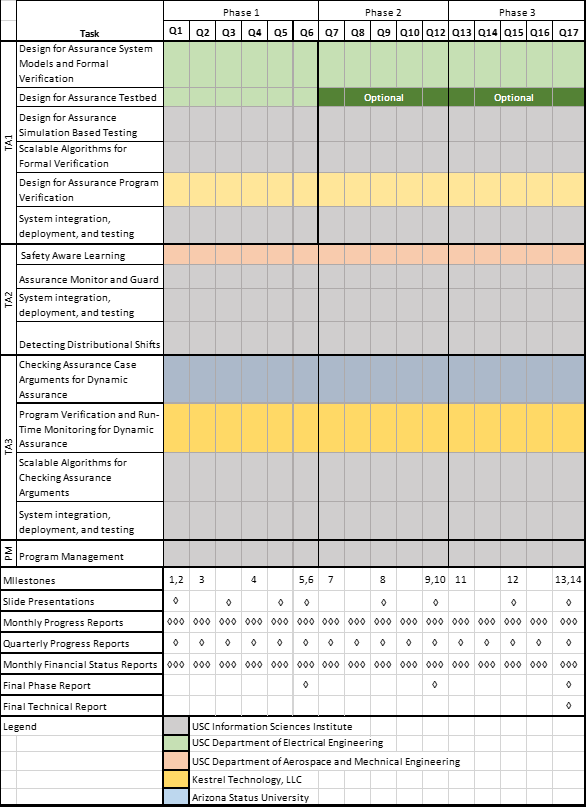
\includegraphics[width=.95\textwidth]{figs/Safeguard_Schedule_V6}
\end{center}
\vspace{-.2in}\caption{Project schedule along with a summary of milestones.  The legend maps task color to organization primary responsible for the task. } 
\label{fig:sandm}
\end{figure}
 

% \section{Level of Effort by Task \textcolor{red}{[Mike/Lisa - 1 pages]}}

% \textcolor{blue}{
% \begin{itemize}
% \item Will be a separate spreadsheet
% \item
% \end{itemize}
% }

\section*{Appendix A: Team Members and Other Information}
\addcontentsline{toc}{section}{Appendix A: Team Members and Other Information}

\baades{This section is mandatory and must include all of the following
components. If a particular subsection is not applicable, state “NONE”.}

\vspace{1ex}

\noindent
\textbf{Team Member Identification}:

\vspace{1ex}

\baades{Provide a list of all team members including the
prime, subcontractor(s), and consultant(s), as applicable. Identify specifically
whether any are a non-US organization or individual, FFRDC and/or Government
entity.}

\begin{centering}

%\small
\begin{tabular}{|p{1.8in}|p{1in}|p{1.1in}|p{0.7in}|p{0.8in}|p{0.7in}|}
\hline
 \textbf{Name} &  \textbf{Role} & \textbf{Organization} & \textbf{Non-US Org?}  & \textbf{Non-US Ind?} &  \textbf{FFRDC or Gov} \\
 \hline
Craig A. Knoblock & Prime & USC & N & N & N\\ \hline
Michael Orosz & Prime & USC & N &  N & N \\ \hline
Satish Thittamaranahalli & Prime & USC & N &  Y & N \\ \hline
Ryan Goodfellow & Prime & USC & N &  N & N \\ \hline
Anoop Kumar & Prime & USC & N & N & N \\ \hline
Satyandra Gupta & Prime & USC & N & N & N \\ \hline
Pierluigi Nuzzo & Prime & USC & N & Y & N \\ \hline
Petros Ioannou & Prime & USC & N & N & N \\ \hline
Chitta Baral & Subcontractor & ASU & N & N & N \\ \hline
Matt Barry & Subcontractor & Kestrel Technology & N & N & N \\ \hline
Douglas Smith & Subcontractor & Kestrel Technology & N & N & N \\ \hline
Henny Sipma & Subcontractor & Kestrel Technology & N & Y & N \\ \hline
\end{tabular} 
\end{centering}

\vspace{1ex}

\noindent
\textbf{Government or FFRDC Team Member Proof of Eligibility to Propose}: NONE

\baades {If
none of the team member organizations (prime or subcontractor) are a
Government entity or FFRDC, state “NONE”.}

\vspace{1ex}

\noindent
\textbf{Government or FFRDC Team Member Statement of Unique Capability}: NONE

\vspace{1ex}

\noindent
\textbf{Organizational Conflict of Interest Affirmations and Disclosure}: NONE

\vspace{1ex}

\noindent
\textbf{Intellectual Property (IP)}: 
\baades {
If no IP restrictions are intended, state “NONE”.
The Government will assume unlimited rights to all IP not explicitly identified as
having less than unlimited rights in the proposal.
For all technical data or computer software that will be furnished to the
Government with other than unlimited rights, provide (per Section VI.B.1) a list
describing all proprietary claims to results, prototypes, deliverables or systems
supporting and/or necessary for the use of the research, results, prototypes
and/or deliverables. Provide documentation proving ownership or possession of
appropriate licensing rights to all patented inventions (or inventions for which a
patent application has been filed) to be used for the proposed project.
}
\begin{centering}

%\small
\begin{tabular}{|p{2.1in}|p{1.2in}|p{1.4in}|p{2in}|}
\hline
\multicolumn{4}{|c|}{COMMERCIAL ITEMS }\\ \hline 
 \textbf{Technical Data, Computer Software To be Furnished With Restrictions} &  \textbf{Basis for Assertion} & \textbf{Asserted Rights Category} & \textbf{Name of Person Asserting Restrictions}  \\  \hline
KT Advance & Developed with mixed funding. & Restricted & David Kulich, Contracts Manager, Kestrel technology, LLC.\\ \hline
\end{tabular} 
\end{centering}

\vspace{1ex}

\noindent
\textbf{Human Subjects Research (HSR)}: NONE

\vspace{1ex}

\noindent
\textbf{Animal Use}: NONE

\vspace{1ex}

\noindent
\textbf{Representations Regarding Unpaid Delinquent Tax Liability or a Felony
Conviction under Any Federal Law}: 
%NONE

\begin{enumerate}
\item
The proposer is  not a corporation that has any unpaid Federal tax liability that has been assessed, for which all judicial and administrative remedies have been exhausted or have lapsed, and that is not being paid in a timely manner pursuant to an agreement with the authority responsible for collecting the tax liability,
\item
The proposer is not a corporation that was convicted of a felony criminal violation under a Federal law within the preceding 24 months.
\end{enumerate}

\vspace{1ex}

\noindent
\textbf{Cost Accounting Standards (CAS) Notices and Certification}:
\baades{
For any proposer who submits a proposal which, if accepted, will result in a CAS-compliant
contract, must include a Disclosure Statement as required by 48 CFR
9903.202. The disclosure forms may be found at
http://www.whitehouse.gov/omb/procurement\_casb
If this section is not applicable, state “NONE”. For further information regarding
this subject, please see www.darpa.mil/work-with-us/additional-baa.
}
NONE


%\section{Appendix B \textcolor{red}{[No Page Count]}}

\section{References}
\bibliographystyle{acm} 
\bibliography{TA3/ta3,TA2/ta2,TA1/ta1}
\end{document}
%%\documentclass[a4paper]{article}
%\documentclass[12pt]{article}
\documentclass[12pt]{dod-blank}

%% Language and font encodings
\usepackage[english]{babel}
\usepackage[utf8x]{inputenc}
\usepackage[T1]{fontenc}

%% Sets page size and margins
%%\usepackage[a4paper,top=3cm,bottom=2cm,left=3cm,right=3cm,marginparwidth=1.75cm]{geometry}
%\usepackage[top=1in, bottom=1in, left=1in, right=1in]{geometry}



%% Useful packages
\usepackage{amsmath}
\usepackage{graphicx}
  \graphicspath{{.}{./image/}}
  \DeclareGraphicsExtensions{.png,.jpg} 
\usepackage[colorinlistoftodos]{todonotes}
\usepackage[colorlinks=true, allcolors=blue]{hyperref}
\usepackage{tabularx}
\usepackage{multirow}
\usepackage{tabulary}
\usepackage{float}
\usepackage{wrapfig}
\usepackage[export]{adjustbox}
\usepackage{comment}
\usepackage{tabularx}
\usepackage{multirow}
\usepackage{tabulary}
\usepackage{enumitem}

\usepackage{listings}
\usepackage{color}
\usepackage{array}
\usepackage{subcaption}
\usepackage{xcolor}




\renewcommand{\textfraction}{0}
\renewcommand{\topfraction}{1.0}
\renewcommand{\bottomfraction}{1.0}

\usepackage{longtable}
%% macros
\newif\iffinal
\finaltrue
\iffinal
  
    \newcommand\baareq[1]{}
    \newcommand\baades[1]{}
 
 
\else
    \definecolor{darkgreen}{rgb}{0,0.4,0}
    \definecolor{darkcyan}{rgb}{0,0.4,0.4}
    \definecolor{darkblue}{rgb}{0,0,0.5}
    
    \newcommand\baareq[1]{{\color{darkcyan}[\textbf{Requirement:} #1]}}
    \newcommand\baades[1]{{\color{darkcyan}[\textbf{Description:} #1]}}
 
\fi




\def\naive{na\"{\i}ve}



\lstset{ 
  backgroundcolor=\color{white},   % choose the background color; you must add \usepackage{color} or \usepackage{xcolor}
  basicstyle=\footnotesize\ttfamily,            % the size of the fonts that are used for the code
  breakatwhitespace=false,         % sets if automatic breaks should only happen at whitespace
  breaklines=true,                 % sets automatic line breaking
  captionpos=b,                    % sets the caption-position to bottom
  commentstyle=\color{mygreen},    % comment style
  % deletekeywords={...},            % if you want to delete keywords from the given language
  escapeinside={\%*}{*)},          % if you want to add LaTeX within your code
  extendedchars=true,              % lets you use non-ASCII characters; for 8-bits encodings only, does not work with UTF-8
  frame=single,	                   % adds a frame around the code
  keepspaces=false,                 % keeps spaces in text, useful for keeping indentation of code (possibly needs columns=flexible)
  keywordstyle=\color{blue}\bfseries\underbar,       % keyword style
  language=Prolog,                 % the language of the code
  % morekeywords={if,and},        % if you want to add more keywords to the set
  numbers=none,                    % where to put the line-numbers; possible values are (none, left, right)
  numbersep=5pt,                   % how far the line-numbers are from the code
  numberstyle=\tiny\color{mygray}, % the style that is used for the line-numbers
  rulecolor=\color{black},         % if not set, the frame-color may be changed on line-breaks within not-black text
  showspaces=false,                % show spaces everywhere adding particular underscores; it overrides 'showstringspaces'
  showstringspaces=false,          % underline spaces within strings only
  showtabs=false,                  % show tabs within strings adding particular underscores
  stepnumber=2,                    % the step between two line-numbers. If it's 1, each line will be numbered
  stringstyle=\color{mymauve},     % string literal style
  tabsize=2,	                   % sets default tabsize to 2 spaces
  title=\lstname                   % show the filename of files included with \lstinputlisting; also try caption instead of title
}

% apply trick for additional keywords for our AC DSL
\lstset{
	emph={for, if, and, or},
    emphstyle={\color{blue}\bfseries\underbar}
}




\title{DARPA Assured Autonomy}
\author{Technical Volume- \textcolor{red}{Thirty-Eight (38) pages max}}

\begin{document}
\pagenumbering{roman}
 
\begin{center}
\large{\textbf{Volume 1: Technical and Management Proposal}}
\end{center}
\textbf{BAA Number:} DARPA-HR001117S0045 \\
\textbf{Technical Area:} TA1, TA2, and TA3 \\
\textbf{Proposal Title:} Assured Autonomy for Learning Enabled Vehicles (Safeguard) \\
\textbf{Lead Institution:} University of Southern California \\
\textbf{Type of organization: } “OTHER EDUCATIONAL” \\

\begin{tabularx}{\linewidth}{XX}

 \textbf{Technical Point of Contact} &  \textbf{Administrative Point of Contact }   \\
Dr.\ Craig A. Knoblock  & Sapphire Masterson  \\ 
USC Information Sciences Institute & USC Dept. of Contracts \& Grants \\
4676 Admiralty Way, Suite 1001 & 4676 Admiralty Way, Suite 1001 \\
Marina del Rey, CA 90292 & Marina del Rey, CA 90292 \\
Tel: 310-448-8786 &  Tel: (310) 448-9161 \\
E-mail: knoblock@isi.edu  & E-mail: sapphirm@usc.edu \\
\end{tabularx}
\\
\\
\textbf{Award instrument requested:}  Procurement Contract, Cost-Reimbursement, No Fee
\\
\\
\textbf{Total amount of the proposed effort:} \$ ...\\
Phase I: \$ ... \\
Phase II: \$ ... \\
Phase III: \$ ... \\
\\
\textbf{Place(s) of performance:} USC, Marina del Rey, CA; Los Angeles, CA;  Tempe, AZ; Palo Alto, CA \\
\textbf{Period(s) of performance:} 04/02/2018 - 03/31/2022     \\
\\
\textbf{Other team members:} \\
\begin{tabularx}{\linewidth}{XX}
Kestrel Technology  & Arizona State University \\
(small business) & (Other Educational)\\
POC: Matthew Barry & POC: Chitta Baral\\
3260 Hillview Avenue & Department of Computer Science and Engr. \\
Palo Alto, CA 94304 & Ira A. Fulton School of Engineering \\ 
phone: (832)205-4876 & Arizona State University\\ 
mrbarry@kestreltechnology.com & Brickyard Suite 572, 699 S. Mill Avenue \\
& Tempe, AZ 85281-8809, U.S.A.\\
& email: chitta@asu.edu\\
\end{tabularx}
\\
\textbf{Proposal validity period: } 180 days\\
\\
\textbf{Data Universal Numbering System (DUNS) number: } 072933393\\
\textbf{Taxpayer identification number:} 95-1642394\\
\textbf{Commercial and Government Entity (CAGE) code:} 1B729 Marina del Rey, CA\\
\textbf{Proposer’s reference number (if any):}  4409-0\\

\newpage
\section{Table of Contents}
\tableofcontents

\newpage
\pagenumbering{arabic}
\section{Executive Summary}
As we rapidly move into a world where machine learning plays a central role in realizing autonomous systems, it is becoming increasingly important to develop techniques that assure that these systems will operate safely and perform as expected. Current approaches are limited to providing assurance for systems with limited or no  learning capabilities. In this context, DARPA's Assured Autonomy BAA seeks to \emph{develop rigorous design and analysis technologies for continual assurance of learning-enabled autonomous systems}. USC in collaboration with Kestrel Technology and ASU is pleased to submit a comprehensive TA1, TA2, and TA3 proposal entitled \emph{``Assured Autonomy for Learning Enabled Vehicles (Safeguard).''} We plan to provide an end-to-end solution to support autonomous systems with learning-enabled components, ranging from design technologies for assurance, to assurance monitoring and control techniques, to representation and online evaluation of assurance cases. We have assembled a strong team of experts that cover the range of technologies that are required to create such an end-to-end system. If successful, the project will provide the technologies for building the next-generation of learning-enabled autonomous systems.  The entire project will take four years and cost \textcolor{red}{\$??}, with an initial version completed at the end of Phase I and successive versions with additional capabilities and improved scalability at the end of Phase II and Phase III.  

In the remainder of this section, we first introduce an  unmanned surface vehicle scenario that will be used throughout the proposal to describe the approach.  Next, we describe our approach to design, monitoring, and dynamic assurance. Finally, we introduce the team involved in the project. 

\textbf{Motivating Scenario.} Consider an autonomous unmanned surface vehicle (USV) guarding a valuable asset in the ocean when an unknown vehicle  approaches the security perimeter, under challenging weather conditions. In this scenario, the USV is required to approach the intruding vehicle, issue a warning signal, and escort it to a safe distance from the controlled area. However, as the USV has no a priori knowledge of its external environment behaviors (e.g., water depth, waves, wind, current, visibility), pre-computing a feasible trajectory, let alone optimal, becomes a non-trivial problem. For trajectory planning, the USV must continuously perform the following tasks:
\begin{itemize}[itemsep=0pt,leftmargin=*]
 \item Sense the current state of the surrounding environment (e.g., water depth, waves, wind, current, visibility) and estimate its own maneuverability constraints (e.g., braking distance, available acceleration, maximum velocity, turning radius, turning rate, safety distance) based on the state of the environment;      
\item Sense the static obstacles in the sensor range and generate a traversability map;
\item Sense the moving obstacles and classify them;   
\item Predict future trajectories of moving obstacles; 
\item Determine if any of the COLREGS \cite{commandant1999international} rules will be in effect with respect to one or more of the nearby vessels and identify the vessels with the right of way.    
\end{itemize}
The above information will be used by the trajectory planner to compute an initial trajectory, which will be continuously refined as the USV gathers additional information.
% It is not possible for the USV to be tested in every possible environment. 
The USV will use learning enabled components to take  decisions as it encounters new situations, such as  
\begin{itemize}[itemsep=0pt,leftmargin=*]
\item Classifiers to identify moving obstacles based on physical appearance and motion signatures,
\item Algorithms to estimate the sensor capabilities in adverse weather conditions,   
\item Algorithms to accurately estimate uncertainty in the environment, 
\item Classifiers to generate traversability maps,
\item Prediction of external vessel behaviors based on motion histories, 
\item Reinforcement learning  to ensure COLREGS compliance of maneuvers,  
\item Algorithms to learning pursuit behaviors.  
\end{itemize}
Learning enabled components will interact with each other in complex ways, where a misclassification error in one component may eventually compromise the entire mission.   
% We will need to make sure that each learning enabled components has a run-time monitor that will ensure that the assumptions made by the learning-enabled component remain valid and prevent erroneous learning. 
% For example, if the vehicle is exhibiting significant error in trajectory tracking, then simply downgrading the trajectory tracking error value may not be a good option.  The failure of prediction of trajectory tracking error might be due to the presence of a significant wake caused by a nearby vessel. The presence of the nearby vessel can be used to explain the degradation in trajectory tracking performance. As the vessel moves away, we can expect the trajectory tracking performance to return to the predicted level.  
While exhaustive validation of learning-enabled cyber-physical systems (LE-CPSs) is a prohibitive task~\cite{Kalra16},
their complexity, heterogeneity, and highly dynamic nature
make it challenging to even leverage existing model-based development techniques to effectively assess system correctness 
% dependability, 
at design time or enforce it at runtime.

\textbf{Design for Assurance.} Safeguard uses a platform-based design approach~\cite{Nuzzo15b} to organize the design process for a LE-CPS and to build assurance cases. Composite models are developed at several levels of abstraction,
from top-level system requirements and safety constraints down to the
implementation level.  Intermediate levels add detail to the levels
above.  The different levels are connected by refinement mappings that
allow properties established at one level to be preserved at the next
level (see Figures~\ref{fig:methodology} and~\ref{fig:assurance}).

Contracts are used to formally specify components and composite models
in terms of (1) Assumptions -- the assumed behaviors of the
environment and the behaviors of other components, and (2) Guarantees
-- the behavior properties that a model guarantees if it operates in a
context that satisfies its assumptions.  A calculus of contracts
allows horizontal composition of contracts to generate contracts for
composite models.  Vertical contracts are used to specify the mapping
or refinement relation between models at different levels of
abstraction.  The system design process starts with a high-level
contract that expresses overall system assumptions and requirements.
Subsequent levels express models with increasing detail until the
lowest level expresses the system in terms of hardware components and
their software controllers.

The assurance case for a CPS arises from the horizontal and vertical
structure of the design in several ways.  The components used within a
particular level are either (1) synthesized using
correct-by-construction design tools together with proofs, (2) derived
statically or dynamically using safety-aware machine-learning
techniques, (3) written manually and verified by analysis tools, or
(4) written manually and validated by extensive testing.  The
assurance case for the whole reflects its compositional structure.  We
anticipate that well-specified contracts together with the calculus of
contracts will eliminate well-known problems with unexpected emergent
behaviors in CPS systems.

The assurance case for the lowest-layer design arises from both the
intra-level assurance and from properties and their proofs that are
preserved under the refinement mapping from the top-level
requirements.  The refinement mappings between model layers will be
constructed using a variety of techniques.  A contract at an abstract
level can be mapped to a component or refined contract by (1)
retrieval of pre-verified components from a platform library, (2)
synthesis using correct-by-construction design and optimization tools,
or (3) manual coding to satisfy a contract.  The mapping of a
composite model will be composed from the mappings of its constituent
components or contracts.  When a composite model cannot be mapped
compositionally to the next level, it will be generated using
correct-by-construction design and optimization tools.

\textbf{Assurance Monitoring and Control.}
We provide an integrated framework for safety-aware learning, assurance monitoring and control, detecting distribution shifts. Three major components offer an efficient TA2 architecture as well as interfaces with TA1 and TA3, that is, (a) safety-aware learning and planning, (b) assurance monitors for guarding architectural and safety constraints; and (c) distribution shift detection.

We will develop a new learning-enabled online decision-making framework that allows opportunistically composing a sequence of actions (maneuvers) to reduce uncertainty in the system capability model without suspending the progress toward the mission goals or compromising safety. Each candidate action is evaluated based on three criteria: (1) the risk of violating a safety constraint using the current uncertainties in the parameter estimates; (2) its relevance to the mission goals; (3)  its expected information gain, i.e., reduction in uncertainty, with respect to the parameter estimates. These evaluations are combined to produce a cumulative mission utility value for each action that drives our learning-enabled decision-making framework. The problem of generating and evaluating sequences of actions can be posed in several way. For example, it can be solved using a branch-and-bound search method like Anytime A*, or formulated with the finite-horizon Markov Decision Process (MDP) framework. We will develop new scalable search strategies to solve this problem efficiently, by potentially evaluating a recent method developed at USC, called FastMap, that can significantly improve the execution time. 

We will develop monitors for architectural and safety constraints. 
% While these constraints can be checked over and over again as sensor information flow in, this naive strategy accounts for a lot of computational overhead. 
To achieve scalability and decrease the overhead, we propose the application of a technique that we currently use in DARPA's RSPACE program, which leverages a physical model of the vehicles dynamics and its interactions with the environment to efficiently determine the readout frequency. We propose two  extensions of this basic idea. First, we will use the theory of Variable Elimination to prioritize which variables to monitor, e.g., controllable, versus uncontrollable, adversarially controlled, or unobservable variables. Second, we invoke the dynamic assessment of assurance cases only when needed. This  decreases the number of times dynamic assessment of assurance cases is initiated as well as the communication bandwidth between the TA2 and TA3 components.

Finally, we will identify a distribution shift by combining statistical and machine learning techniques to differentiate between environmental and sensor changes. We will exploit a categorization of the shifts based on their cause and duration as well as extend our earlier work on detecting and mitigating sensor failures for all types of monitored variables.  

\textbf{Dynamic Assurance:} The Safeguard {\em design for assurance\/} activity takes a systems-theoretic stance toward safety.  Consequently, it presumes that safety is an emergent property of the system, and that hazards can present themselves through unintended interactions and performance violations in addition to causal events such as component failures.  Our design approach includes consideration of intent as well as hazard analysis and mitigation.  The artifacts from these activities populate contracts and assumptions for the dynamic assurance case.  
We thus build safety into the product by working at a systems-level viewpoint, using lexicon and design patterns familiar to both hardware and software engineers; safety is an emergent property of the system, not an afterthought.  
As system behavior evolves during runtime owing to learning, threats, degradation, or some other factor, the dynamic assurance case identifies whether the safety constraints continue to be satisfied.  If not, it provides notifications or issues recovery instructions directly from a lookup table.

Our implementation of the dynamic assurance case employs a declarative knowledge base inference engine and a domain-specific language tailored to our approach.  We have used them successfully for assurance case tool sets and arguments, and will extend them to reason about uncertainty and learning.  Our approach to achieve scalability is to specialize solvers toward modularity and to take advantage of domain knowledge.  Specifically, we will develop answer set programming techniques for context-dependent learning for reasoning about the learning-enabled components as well as learning assurance rules.  We will develop new formalisms for uncertainty to include causality, using weights for computing probabilities, and probabilistic non-monotonicity.  To achieve scaling objectives we will implement specializations using modularity, weighted CSPs, and message passing. 

% The system safety constraints revealed from that design become the key elements of our dynamic assurance case.  Our verification tools ensure the constraints are relevant, identifiable, and their implementation and effect observable.  

\textbf{Team.} We have assembled a team that is exceptionally well-qualified to build the proposed Safeguard system.  The team will be led by Dr.\ Craig Knoblock, the Principal Investigator for the effort, who currently leads the Intelligent Systems Division at the Information Sciences Institute.  He has led many large DARPA and IARPA projects over the years and has a strong track record in conducting leading edge research and then transitioning the technology to commercial use.  He will be supported by Dr.\ Michael Orosz as the Project Manager, who also has  experience in managing large research projects and on autonomous systems.  The TA1 team will be led by Dr.\ Pierluigi Nuzzo, who is an expert in embedded system design methodologies and the  application of formal methods to cyber-physical systems.  The TA1 team also includes Dr.\ Doug Smith, who has spent many years working on scalable correct-by-construction techniques and Dr.\ Henny Sipma, who has significant experience in applying program verification methods to real-world problems.  The TA1 team also includes Ryan Goodfellow, who has done a large amount of work on simulation-based testing.  The TA2 team will be led by Dr.\ Knoblock who has worked on topics related to both monitoring and detecting distribution changes.  He will be supported by Dr.\ Satyandra Gupta, who is an expert on autonomous surface vehicles as well as on safety-aware learning. He will also be supported by Drs.\ Anoop Kumar and Satish Thittamaranahalli, who have also previously worked on efficient methods for execution monitoring.  The TA3 team will be lead by Dr.\ Matthew Barry, who has experience in creating the technologies for assurance cases.  He will be supported by Dr.\ Chitta Baral, who is an expert on ASP solvers and by Dr.\ Thittamaranahalli who is an expert on SAT solvers, both of which will be applied to provide scalable assurance case reasoning.  Finally, Dr.\ Petros Ioannou, who is an expert on control systems for autonomous vehicles will provide an autonomous vehicle platform, which will form the focus of our work until the TA4 teams provide additional vehicle platforms for development.  

\newpage
\section{Innovative Claims and Deliverables}

In this project we will develop and build an end-to-end system for assured autonomy.  This section describes the key innovations by technical area and then the overall deliverables of the project.

\paragraph{Design for Assurance}

\begin{itemize}[itemsep=0pt,leftmargin=*]
\item We address the LE-CPS design challenges via a holistic approach that can contextually generate design artifacts and assurance cases. We develop a compositional, contract-based modeling framework, methods, and tools to support the design process from system-level requirement capture,  formalization, and analysis, to the generation, testing, and continual monitoring of software and hardware artifacts in feedback loop with a physical process.

\item We develop compositional abstractions and interfaces (vertical contracts) that can  bridge heterogeneous formalisms and heterogeneous decomposition architectures to make system analysis and synthesis tractable, consistently combine different verification and synthesis methods at design time, and provide seamless support for dynamic assurance at run time. %We aim to quantitatively capture the confidence in the satisfaction of requirements under uncertain or unknown conditions, and resilience properties of  systems at different abstraction levels, to enable trade-off evaluation between resilience, performance, and cost.

\item We develop a unifying framework and efficient algorithms to reason about the combination of discrete and continuous dynamics and constraints in the presence of uncertainties in LE-CPS using a satisfiability modulo convex approach~\cite{Shoukry2017} for contract-based system verification and scalable trajectory planning.  

\item We provide an environment for high-fidelity CPS testing, in which production-ready software, e.g.,  safety-critical learning and control, may be deployed and tested 
% by extending the Cypress testbed environment \cite{Goodfellow2015Cypress:Systems} 
with time dilation facilities, so that it synchronizes with a physical simulation that is not necessarily running in real time, while still having the perception of real time.

\item We 
% These facilities allow a cyber system to be  
propose an approach for unanticipated behavior space identification and test coverage maximization which leverages results from the theory of differential algebraic equation (DAE)~\cite{Berger2013ControllabilitySurvey,Ilchmann2005ATheory,BergerOnSystems,Lamour2013} 
to prune the behavior search space and identify smaller regions of interest for efficient simulation-based testing. 
% We then compute the intersection of these two behavior spaces and restrict our simulation based testing search space to this subspace.
\end{itemize}

\paragraph{Assurance Monitoring and Control}

\begin{itemize}[itemsep=0pt,leftmargin=*]
\item 
%We integrate safety-aware learning into the overall decision making problem. The goal is to maximize mission utility without violating the safety constraints. 
Our safety-aware learning framework enables the system to opportunistically select and execute actions to assist the learning-enabled component in reducing model uncertainty without compromising safety or deviating from the mission goals. The value of uncertainty reduction is explicitly incorporated in the optimization process for selecting the best action.  
\item For safety-aware learning, we propose the idea of preprocessing the search space of the problem domain before queries and observations come in. With such a linear-time preprocessing phase, the performance of search and optimization algorithms can be significantly boosted. For example, in regular A* search, the intensional or extensional search space can be preprocessed in near-linear time to yield an embedding of each state as a point in Euclidean space~\cite{cujakk}. Then, when the query comes in, A* search can make use of these Euclidean distances as heuristic distances between two states to yield order-of-magnitude speedups. 
%In Anytime A* for safety-aware learning and planning, this leads to a significantly better quality of actions chosen within a time limit, and in the MDP framework, the same ideas can be used to improve the convergence of Bellman updates for safety-aware Reinforcement Learning.
\item As massive amounts of sensor information flow in, it is imperative for us to efficiently process this information for monitoring architectural and safety constraints. Building on our past work on similar tasks, we propose novel technologies for efficiently monitoring constraints. These algorithms can yield an exponential reduction in the amount of sensor data that needs to be processed. Doing this also reduces the message complexities between the various modules. %We also propose to use the theory of Variable Elimination (VE) to monitor constraints with uncontrollable, adversarially controlled, and/or unobservable variables. VE yields a substrate constraint to monitor that characterizes a dominant strategy of the controllable variables over the uncontrollable, adversarially controlled, and/or unobservable variables.
\item We will develop techniques to identify  distributional shifts and determine the underlying cause (e.g., change in environment, sensor failure,   etc.), as well as strategies for handling the various distributional shifts.   Notably, we propose to build on our past work and use compact representations to exploit historical data to identify distributional shifts.
\end{itemize}

\paragraph{Dynamic Assurance}

\begin{itemize}[itemsep=0pt,leftmargin=*]

\item We demonstrate the integration of dynamic assurance for safety-critical learning-enabled dynamic systems in which evolutionary behaviors are expected and tolerated as a property of the functionality.   The impact will be consequential contributions safety-critical dynamic systems in which evolutionary behaviors are expected and tolerated as portion of the functionality.   
\item We implement dynamic assurance by combining features of system safety, formal methods, logic programming, uncertain reasoning, and domain-specific languages.  We populate assurance case arguments at several levels of modeling and implementation abstraction, using the analysis results to produce design-time evidence supporting assurance claims.  
%We provide automated reasoning about the assurance case itself to produce verification, consistency, and completeness results for the argument.  Dynamic assurance results then yield trusted explanations of whether safety constraints and assumptions and other contracts still hold during the collection of runtime evidence from monitors. 
\item We develop and demonstrate ASP formalisms crucial to applications in dynamic assurance. We demonstrate the suitability of the technology especially for assurance case arguments owing to the improved legibility, consistency and completeness checks, handling of uncertain and default reasoning, and scalability.  
%We will produce modularized solvers for enhanced performance based on recent algorithmic developments in exploiting structure, kernelization, and message passing. We provide a formalism to enable learning of assurance rules. 
We provide a novel approach to handling uncertainty that provides the ability to do causal and counter-factual reasoning as well as probabilistic non-monotonicity.  Overcoming limitations of traditional inductive logic techniques, we develop a novel iterative and incremental approach based on context dependent learning. 
\end{itemize}

\paragraph{Deliverables}
During the course of this project, we will build and deliver a fully-operational system that covers all three of the technical areas.  The detailed capabilities of this system are described in the individual technical sections.  The resulting system will be available as open source under a permissive license, which will allow other organizations to use the work, extend it in new directions, and even commercialize the software.  Kestrel Technology has significant experience in this space and has built and applied these types of technologies to a variety of real world tasks.  Kestrel is ideally suited to pursue commercial uses of this technology and the permissive license will facilitate exploring these opportunities since there will be no need to negotiate intellectual property rights.  

\newpage
\section{Technical Plan}
%%\documentclass[a4paper]{article}
%\documentclass[12pt]{article}
\documentclass[12pt]{dod-blank}

%% Language and font encodings
\usepackage[english]{babel}
\usepackage[utf8x]{inputenc}
\usepackage[T1]{fontenc}

%% Sets page size and margins
%%\usepackage[a4paper,top=3cm,bottom=2cm,left=3cm,right=3cm,marginparwidth=1.75cm]{geometry}
%\usepackage[top=1in, bottom=1in, left=1in, right=1in]{geometry}



%% Useful packages
\usepackage{amsmath}
\usepackage{graphicx}
  \graphicspath{{.}{./image/}}
  \DeclareGraphicsExtensions{.png,.jpg} 
\usepackage[colorinlistoftodos]{todonotes}
\usepackage[colorlinks=true, allcolors=blue]{hyperref}
\usepackage{tabularx}
\usepackage{multirow}
\usepackage{tabulary}
\usepackage{float}
\usepackage{wrapfig}
\usepackage[export]{adjustbox}
\usepackage{comment}
\usepackage{tabularx}
\usepackage{multirow}
\usepackage{tabulary}
\usepackage{enumitem}

\usepackage{listings}
\usepackage{color}
\usepackage{array}
\usepackage{subcaption}
\usepackage{xcolor}




\renewcommand{\textfraction}{0}
\renewcommand{\topfraction}{1.0}
\renewcommand{\bottomfraction}{1.0}

\usepackage{longtable}
%% macros
\newif\iffinal
\finaltrue
\iffinal
  
    \newcommand\baareq[1]{}
    \newcommand\baades[1]{}
 
 
\else
    \definecolor{darkgreen}{rgb}{0,0.4,0}
    \definecolor{darkcyan}{rgb}{0,0.4,0.4}
    \definecolor{darkblue}{rgb}{0,0,0.5}
    
    \newcommand\baareq[1]{{\color{darkcyan}[\textbf{Requirement:} #1]}}
    \newcommand\baades[1]{{\color{darkcyan}[\textbf{Description:} #1]}}
 
\fi




\def\naive{na\"{\i}ve}



\lstset{ 
  backgroundcolor=\color{white},   % choose the background color; you must add \usepackage{color} or \usepackage{xcolor}
  basicstyle=\footnotesize\ttfamily,            % the size of the fonts that are used for the code
  breakatwhitespace=false,         % sets if automatic breaks should only happen at whitespace
  breaklines=true,                 % sets automatic line breaking
  captionpos=b,                    % sets the caption-position to bottom
  commentstyle=\color{mygreen},    % comment style
  % deletekeywords={...},            % if you want to delete keywords from the given language
  escapeinside={\%*}{*)},          % if you want to add LaTeX within your code
  extendedchars=true,              % lets you use non-ASCII characters; for 8-bits encodings only, does not work with UTF-8
  frame=single,	                   % adds a frame around the code
  keepspaces=false,                 % keeps spaces in text, useful for keeping indentation of code (possibly needs columns=flexible)
  keywordstyle=\color{blue}\bfseries\underbar,       % keyword style
  language=Prolog,                 % the language of the code
  % morekeywords={if,and},        % if you want to add more keywords to the set
  numbers=none,                    % where to put the line-numbers; possible values are (none, left, right)
  numbersep=5pt,                   % how far the line-numbers are from the code
  numberstyle=\tiny\color{mygray}, % the style that is used for the line-numbers
  rulecolor=\color{black},         % if not set, the frame-color may be changed on line-breaks within not-black text
  showspaces=false,                % show spaces everywhere adding particular underscores; it overrides 'showstringspaces'
  showstringspaces=false,          % underline spaces within strings only
  showtabs=false,                  % show tabs within strings adding particular underscores
  stepnumber=2,                    % the step between two line-numbers. If it's 1, each line will be numbered
  stringstyle=\color{mymauve},     % string literal style
  tabsize=2,	                   % sets default tabsize to 2 spaces
  title=\lstname                   % show the filename of files included with \lstinputlisting; also try caption instead of title
}

% apply trick for additional keywords for our AC DSL
\lstset{
	emph={for, if, and, or},
    emphstyle={\color{blue}\bfseries\underbar}
}




\title{DARPA Assured Autonomy}
\author{Technical Volume- \textcolor{red}{Thirty-Eight (38) pages max}}

\begin{document}
\pagenumbering{roman}
\include{cover}

\newpage
\section{Table of Contents}
\tableofcontents

\newpage
\pagenumbering{arabic}
\section{Executive Summary}
As we rapidly move into a world where machine learning plays a central role in realizing autonomous systems, it is becoming increasingly important to develop techniques that assure that these systems will operate safely and perform as expected. Current approaches are limited to providing assurance for systems with limited or no  learning capabilities. In this context, DARPA's Assured Autonomy BAA seeks to \emph{develop rigorous design and analysis technologies for continual assurance of learning-enabled autonomous systems}. USC in collaboration with Kestrel Technology and ASU is pleased to submit a comprehensive TA1, TA2, and TA3 proposal entitled \emph{``Assured Autonomy for Learning Enabled Vehicles (Safeguard).''} We plan to provide an end-to-end solution to support autonomous systems with learning-enabled components, ranging from design technologies for assurance, to assurance monitoring and control techniques, to representation and online evaluation of assurance cases. We have assembled a strong team of experts that cover the range of technologies that are required to create such an end-to-end system. If successful, the project will provide the technologies for building the next-generation of learning-enabled autonomous systems.  The entire project will take four years and cost \textcolor{red}{\$??}, with an initial version completed at the end of Phase I and successive versions with additional capabilities and improved scalability at the end of Phase II and Phase III.  

In the remainder of this section, we first introduce an  unmanned surface vehicle scenario that will be used throughout the proposal to describe the approach.  Next, we describe our approach to design, monitoring, and dynamic assurance. Finally, we introduce the team involved in the project. 

\textbf{Motivating Scenario.} Consider an autonomous unmanned surface vehicle (USV) guarding a valuable asset in the ocean when an unknown vehicle  approaches the security perimeter, under challenging weather conditions. In this scenario, the USV is required to approach the intruding vehicle, issue a warning signal, and escort it to a safe distance from the controlled area. However, as the USV has no a priori knowledge of its external environment behaviors (e.g., water depth, waves, wind, current, visibility), pre-computing a feasible trajectory, let alone optimal, becomes a non-trivial problem. For trajectory planning, the USV must continuously perform the following tasks:
\begin{itemize}[itemsep=0pt,leftmargin=*]
 \item Sense the current state of the surrounding environment (e.g., water depth, waves, wind, current, visibility) and estimate its own maneuverability constraints (e.g., braking distance, available acceleration, maximum velocity, turning radius, turning rate, safety distance) based on the state of the environment;      
\item Sense the static obstacles in the sensor range and generate a traversability map;
\item Sense the moving obstacles and classify them;   
\item Predict future trajectories of moving obstacles; 
\item Determine if any of the COLREGS \cite{commandant1999international} rules will be in effect with respect to one or more of the nearby vessels and identify the vessels with the right of way.    
\end{itemize}
The above information will be used by the trajectory planner to compute an initial trajectory, which will be continuously refined as the USV gathers additional information.
% It is not possible for the USV to be tested in every possible environment. 
The USV will use learning enabled components to take  decisions as it encounters new situations, such as  
\begin{itemize}[itemsep=0pt,leftmargin=*]
\item Classifiers to identify moving obstacles based on physical appearance and motion signatures,
\item Algorithms to estimate the sensor capabilities in adverse weather conditions,   
\item Algorithms to accurately estimate uncertainty in the environment, 
\item Classifiers to generate traversability maps,
\item Prediction of external vessel behaviors based on motion histories, 
\item Reinforcement learning  to ensure COLREGS compliance of maneuvers,  
\item Algorithms to learning pursuit behaviors.  
\end{itemize}
Learning enabled components will interact with each other in complex ways, where a misclassification error in one component may eventually compromise the entire mission.   
% We will need to make sure that each learning enabled components has a run-time monitor that will ensure that the assumptions made by the learning-enabled component remain valid and prevent erroneous learning. 
% For example, if the vehicle is exhibiting significant error in trajectory tracking, then simply downgrading the trajectory tracking error value may not be a good option.  The failure of prediction of trajectory tracking error might be due to the presence of a significant wake caused by a nearby vessel. The presence of the nearby vessel can be used to explain the degradation in trajectory tracking performance. As the vessel moves away, we can expect the trajectory tracking performance to return to the predicted level.  
While exhaustive validation of learning-enabled cyber-physical systems (LE-CPSs) is a prohibitive task~\cite{Kalra16},
their complexity, heterogeneity, and highly dynamic nature
make it challenging to even leverage existing model-based development techniques to effectively assess system correctness 
% dependability, 
at design time or enforce it at runtime.

\textbf{Design for Assurance.} Safeguard uses a platform-based design approach~\cite{Nuzzo15b} to organize the design process for a LE-CPS and to build assurance cases. Composite models are developed at several levels of abstraction,
from top-level system requirements and safety constraints down to the
implementation level.  Intermediate levels add detail to the levels
above.  The different levels are connected by refinement mappings that
allow properties established at one level to be preserved at the next
level (see Figures~\ref{fig:methodology} and~\ref{fig:assurance}).

Contracts are used to formally specify components and composite models
in terms of (1) Assumptions -- the assumed behaviors of the
environment and the behaviors of other components, and (2) Guarantees
-- the behavior properties that a model guarantees if it operates in a
context that satisfies its assumptions.  A calculus of contracts
allows horizontal composition of contracts to generate contracts for
composite models.  Vertical contracts are used to specify the mapping
or refinement relation between models at different levels of
abstraction.  The system design process starts with a high-level
contract that expresses overall system assumptions and requirements.
Subsequent levels express models with increasing detail until the
lowest level expresses the system in terms of hardware components and
their software controllers.

The assurance case for a CPS arises from the horizontal and vertical
structure of the design in several ways.  The components used within a
particular level are either (1) synthesized using
correct-by-construction design tools together with proofs, (2) derived
statically or dynamically using safety-aware machine-learning
techniques, (3) written manually and verified by analysis tools, or
(4) written manually and validated by extensive testing.  The
assurance case for the whole reflects its compositional structure.  We
anticipate that well-specified contracts together with the calculus of
contracts will eliminate well-known problems with unexpected emergent
behaviors in CPS systems.

The assurance case for the lowest-layer design arises from both the
intra-level assurance and from properties and their proofs that are
preserved under the refinement mapping from the top-level
requirements.  The refinement mappings between model layers will be
constructed using a variety of techniques.  A contract at an abstract
level can be mapped to a component or refined contract by (1)
retrieval of pre-verified components from a platform library, (2)
synthesis using correct-by-construction design and optimization tools,
or (3) manual coding to satisfy a contract.  The mapping of a
composite model will be composed from the mappings of its constituent
components or contracts.  When a composite model cannot be mapped
compositionally to the next level, it will be generated using
correct-by-construction design and optimization tools.

\textbf{Assurance Monitoring and Control.}
We provide an integrated framework for safety-aware learning, assurance monitoring and control, detecting distribution shifts. Three major components offer an efficient TA2 architecture as well as interfaces with TA1 and TA3, that is, (a) safety-aware learning and planning, (b) assurance monitors for guarding architectural and safety constraints; and (c) distribution shift detection.

We will develop a new learning-enabled online decision-making framework that allows opportunistically composing a sequence of actions (maneuvers) to reduce uncertainty in the system capability model without suspending the progress toward the mission goals or compromising safety. Each candidate action is evaluated based on three criteria: (1) the risk of violating a safety constraint using the current uncertainties in the parameter estimates; (2) its relevance to the mission goals; (3)  its expected information gain, i.e., reduction in uncertainty, with respect to the parameter estimates. These evaluations are combined to produce a cumulative mission utility value for each action that drives our learning-enabled decision-making framework. The problem of generating and evaluating sequences of actions can be posed in several way. For example, it can be solved using a branch-and-bound search method like Anytime A*, or formulated with the finite-horizon Markov Decision Process (MDP) framework. We will develop new scalable search strategies to solve this problem efficiently, by potentially evaluating a recent method developed at USC, called FastMap, that can significantly improve the execution time. 

We will develop monitors for architectural and safety constraints. 
% While these constraints can be checked over and over again as sensor information flow in, this naive strategy accounts for a lot of computational overhead. 
To achieve scalability and decrease the overhead, we propose the application of a technique that we currently use in DARPA's RSPACE program, which leverages a physical model of the vehicles dynamics and its interactions with the environment to efficiently determine the readout frequency. We propose two  extensions of this basic idea. First, we will use the theory of Variable Elimination to prioritize which variables to monitor, e.g., controllable, versus uncontrollable, adversarially controlled, or unobservable variables. Second, we invoke the dynamic assessment of assurance cases only when needed. This  decreases the number of times dynamic assessment of assurance cases is initiated as well as the communication bandwidth between the TA2 and TA3 components.

Finally, we will identify a distribution shift by combining statistical and machine learning techniques to differentiate between environmental and sensor changes. We will exploit a categorization of the shifts based on their cause and duration as well as extend our earlier work on detecting and mitigating sensor failures for all types of monitored variables.  

\textbf{Dynamic Assurance:} The Safeguard {\em design for assurance\/} activity takes a systems-theoretic stance toward safety.  Consequently, it presumes that safety is an emergent property of the system, and that hazards can present themselves through unintended interactions and performance violations in addition to causal events such as component failures.  Our design approach includes consideration of intent as well as hazard analysis and mitigation.  The artifacts from these activities populate contracts and assumptions for the dynamic assurance case.  
We thus build safety into the product by working at a systems-level viewpoint, using lexicon and design patterns familiar to both hardware and software engineers; safety is an emergent property of the system, not an afterthought.  
As system behavior evolves during runtime owing to learning, threats, degradation, or some other factor, the dynamic assurance case identifies whether the safety constraints continue to be satisfied.  If not, it provides notifications or issues recovery instructions directly from a lookup table.

Our implementation of the dynamic assurance case employs a declarative knowledge base inference engine and a domain-specific language tailored to our approach.  We have used them successfully for assurance case tool sets and arguments, and will extend them to reason about uncertainty and learning.  Our approach to achieve scalability is to specialize solvers toward modularity and to take advantage of domain knowledge.  Specifically, we will develop answer set programming techniques for context-dependent learning for reasoning about the learning-enabled components as well as learning assurance rules.  We will develop new formalisms for uncertainty to include causality, using weights for computing probabilities, and probabilistic non-monotonicity.  To achieve scaling objectives we will implement specializations using modularity, weighted CSPs, and message passing. 

% The system safety constraints revealed from that design become the key elements of our dynamic assurance case.  Our verification tools ensure the constraints are relevant, identifiable, and their implementation and effect observable.  

\textbf{Team.} We have assembled a team that is exceptionally well-qualified to build the proposed Safeguard system.  The team will be led by Dr.\ Craig Knoblock, the Principal Investigator for the effort, who currently leads the Intelligent Systems Division at the Information Sciences Institute.  He has led many large DARPA and IARPA projects over the years and has a strong track record in conducting leading edge research and then transitioning the technology to commercial use.  He will be supported by Dr.\ Michael Orosz as the Project Manager, who also has  experience in managing large research projects and on autonomous systems.  The TA1 team will be led by Dr.\ Pierluigi Nuzzo, who is an expert in embedded system design methodologies and the  application of formal methods to cyber-physical systems.  The TA1 team also includes Dr.\ Doug Smith, who has spent many years working on scalable correct-by-construction techniques and Dr.\ Henny Sipma, who has significant experience in applying program verification methods to real-world problems.  The TA1 team also includes Ryan Goodfellow, who has done a large amount of work on simulation-based testing.  The TA2 team will be led by Dr.\ Knoblock who has worked on topics related to both monitoring and detecting distribution changes.  He will be supported by Dr.\ Satyandra Gupta, who is an expert on autonomous surface vehicles as well as on safety-aware learning. He will also be supported by Drs.\ Anoop Kumar and Satish Thittamaranahalli, who have also previously worked on efficient methods for execution monitoring.  The TA3 team will be lead by Dr.\ Matthew Barry, who has experience in creating the technologies for assurance cases.  He will be supported by Dr.\ Chitta Baral, who is an expert on ASP solvers and by Dr.\ Thittamaranahalli who is an expert on SAT solvers, both of which will be applied to provide scalable assurance case reasoning.  Finally, Dr.\ Petros Ioannou, who is an expert on control systems for autonomous vehicles will provide an autonomous vehicle platform, which will form the focus of our work until the TA4 teams provide additional vehicle platforms for development.  

\newpage
\section{Innovative Claims and Deliverables}

In this project we will develop and build an end-to-end system for assured autonomy.  This section describes the key innovations by technical area and then the overall deliverables of the project.

\paragraph{Design for Assurance}

\begin{itemize}[itemsep=0pt,leftmargin=*]
\item We address the LE-CPS design challenges via a holistic approach that can contextually generate design artifacts and assurance cases. We develop a compositional, contract-based modeling framework, methods, and tools to support the design process from system-level requirement capture,  formalization, and analysis, to the generation, testing, and continual monitoring of software and hardware artifacts in feedback loop with a physical process.

\item We develop compositional abstractions and interfaces (vertical contracts) that can  bridge heterogeneous formalisms and heterogeneous decomposition architectures to make system analysis and synthesis tractable, consistently combine different verification and synthesis methods at design time, and provide seamless support for dynamic assurance at run time. %We aim to quantitatively capture the confidence in the satisfaction of requirements under uncertain or unknown conditions, and resilience properties of  systems at different abstraction levels, to enable trade-off evaluation between resilience, performance, and cost.

\item We develop a unifying framework and efficient algorithms to reason about the combination of discrete and continuous dynamics and constraints in the presence of uncertainties in LE-CPS using a satisfiability modulo convex approach~\cite{Shoukry2017} for contract-based system verification and scalable trajectory planning.  

\item We provide an environment for high-fidelity CPS testing, in which production-ready software, e.g.,  safety-critical learning and control, may be deployed and tested 
% by extending the Cypress testbed environment \cite{Goodfellow2015Cypress:Systems} 
with time dilation facilities, so that it synchronizes with a physical simulation that is not necessarily running in real time, while still having the perception of real time.

\item We 
% These facilities allow a cyber system to be  
propose an approach for unanticipated behavior space identification and test coverage maximization which leverages results from the theory of differential algebraic equation (DAE)~\cite{Berger2013ControllabilitySurvey,Ilchmann2005ATheory,BergerOnSystems,Lamour2013} 
to prune the behavior search space and identify smaller regions of interest for efficient simulation-based testing. 
% We then compute the intersection of these two behavior spaces and restrict our simulation based testing search space to this subspace.
\end{itemize}

\paragraph{Assurance Monitoring and Control}

\begin{itemize}[itemsep=0pt,leftmargin=*]
\item 
%We integrate safety-aware learning into the overall decision making problem. The goal is to maximize mission utility without violating the safety constraints. 
Our safety-aware learning framework enables the system to opportunistically select and execute actions to assist the learning-enabled component in reducing model uncertainty without compromising safety or deviating from the mission goals. The value of uncertainty reduction is explicitly incorporated in the optimization process for selecting the best action.  
\item For safety-aware learning, we propose the idea of preprocessing the search space of the problem domain before queries and observations come in. With such a linear-time preprocessing phase, the performance of search and optimization algorithms can be significantly boosted. For example, in regular A* search, the intensional or extensional search space can be preprocessed in near-linear time to yield an embedding of each state as a point in Euclidean space~\cite{cujakk}. Then, when the query comes in, A* search can make use of these Euclidean distances as heuristic distances between two states to yield order-of-magnitude speedups. 
%In Anytime A* for safety-aware learning and planning, this leads to a significantly better quality of actions chosen within a time limit, and in the MDP framework, the same ideas can be used to improve the convergence of Bellman updates for safety-aware Reinforcement Learning.
\item As massive amounts of sensor information flow in, it is imperative for us to efficiently process this information for monitoring architectural and safety constraints. Building on our past work on similar tasks, we propose novel technologies for efficiently monitoring constraints. These algorithms can yield an exponential reduction in the amount of sensor data that needs to be processed. Doing this also reduces the message complexities between the various modules. %We also propose to use the theory of Variable Elimination (VE) to monitor constraints with uncontrollable, adversarially controlled, and/or unobservable variables. VE yields a substrate constraint to monitor that characterizes a dominant strategy of the controllable variables over the uncontrollable, adversarially controlled, and/or unobservable variables.
\item We will develop techniques to identify  distributional shifts and determine the underlying cause (e.g., change in environment, sensor failure,   etc.), as well as strategies for handling the various distributional shifts.   Notably, we propose to build on our past work and use compact representations to exploit historical data to identify distributional shifts.
\end{itemize}

\paragraph{Dynamic Assurance}

\begin{itemize}[itemsep=0pt,leftmargin=*]

\item We demonstrate the integration of dynamic assurance for safety-critical learning-enabled dynamic systems in which evolutionary behaviors are expected and tolerated as a property of the functionality.   The impact will be consequential contributions safety-critical dynamic systems in which evolutionary behaviors are expected and tolerated as portion of the functionality.   
\item We implement dynamic assurance by combining features of system safety, formal methods, logic programming, uncertain reasoning, and domain-specific languages.  We populate assurance case arguments at several levels of modeling and implementation abstraction, using the analysis results to produce design-time evidence supporting assurance claims.  
%We provide automated reasoning about the assurance case itself to produce verification, consistency, and completeness results for the argument.  Dynamic assurance results then yield trusted explanations of whether safety constraints and assumptions and other contracts still hold during the collection of runtime evidence from monitors. 
\item We develop and demonstrate ASP formalisms crucial to applications in dynamic assurance. We demonstrate the suitability of the technology especially for assurance case arguments owing to the improved legibility, consistency and completeness checks, handling of uncertain and default reasoning, and scalability.  
%We will produce modularized solvers for enhanced performance based on recent algorithmic developments in exploiting structure, kernelization, and message passing. We provide a formalism to enable learning of assurance rules. 
We provide a novel approach to handling uncertainty that provides the ability to do causal and counter-factual reasoning as well as probabilistic non-monotonicity.  Overcoming limitations of traditional inductive logic techniques, we develop a novel iterative and incremental approach based on context dependent learning. 
\end{itemize}

\paragraph{Deliverables}
During the course of this project, we will build and deliver a fully-operational system that covers all three of the technical areas.  The detailed capabilities of this system are described in the individual technical sections.  The resulting system will be available as open source under a permissive license, which will allow other organizations to use the work, extend it in new directions, and even commercialize the software.  Kestrel Technology has significant experience in this space and has built and applied these types of technologies to a variety of real world tasks.  Kestrel is ideally suited to pursue commercial uses of this technology and the permissive license will facilitate exploring these opportunities since there will be no need to negotiate intellectual property rights.  

\newpage
\section{Technical Plan}
\input{./TA1/main}
\input{./TA2/main}
\input{./TA3/main}
\clearpage
\newpage


\section{Management Plan}


The Principal Investigator for this effort is Dr. Craig Knoblock who is responsible for all aspects of the effort, will coordinate the parallel team efforts, and will ensure high levels of performance from individual team members.  The Co-P/I, Dr. Michael Orosz, will provide project management and will assist all performers in the execution of the project.    The project team is divided into three working groups (Figure~\ref{fig:org_chart}) corresponding to Technical Areas 1-3, however, members of each team contribute across all project activities.   Table~\ref{fig:Table_Mgmt} defines the major contributions of each project team member to the project tasks.

\begin{figure}[tbhp]
%\vspace{-25pt}
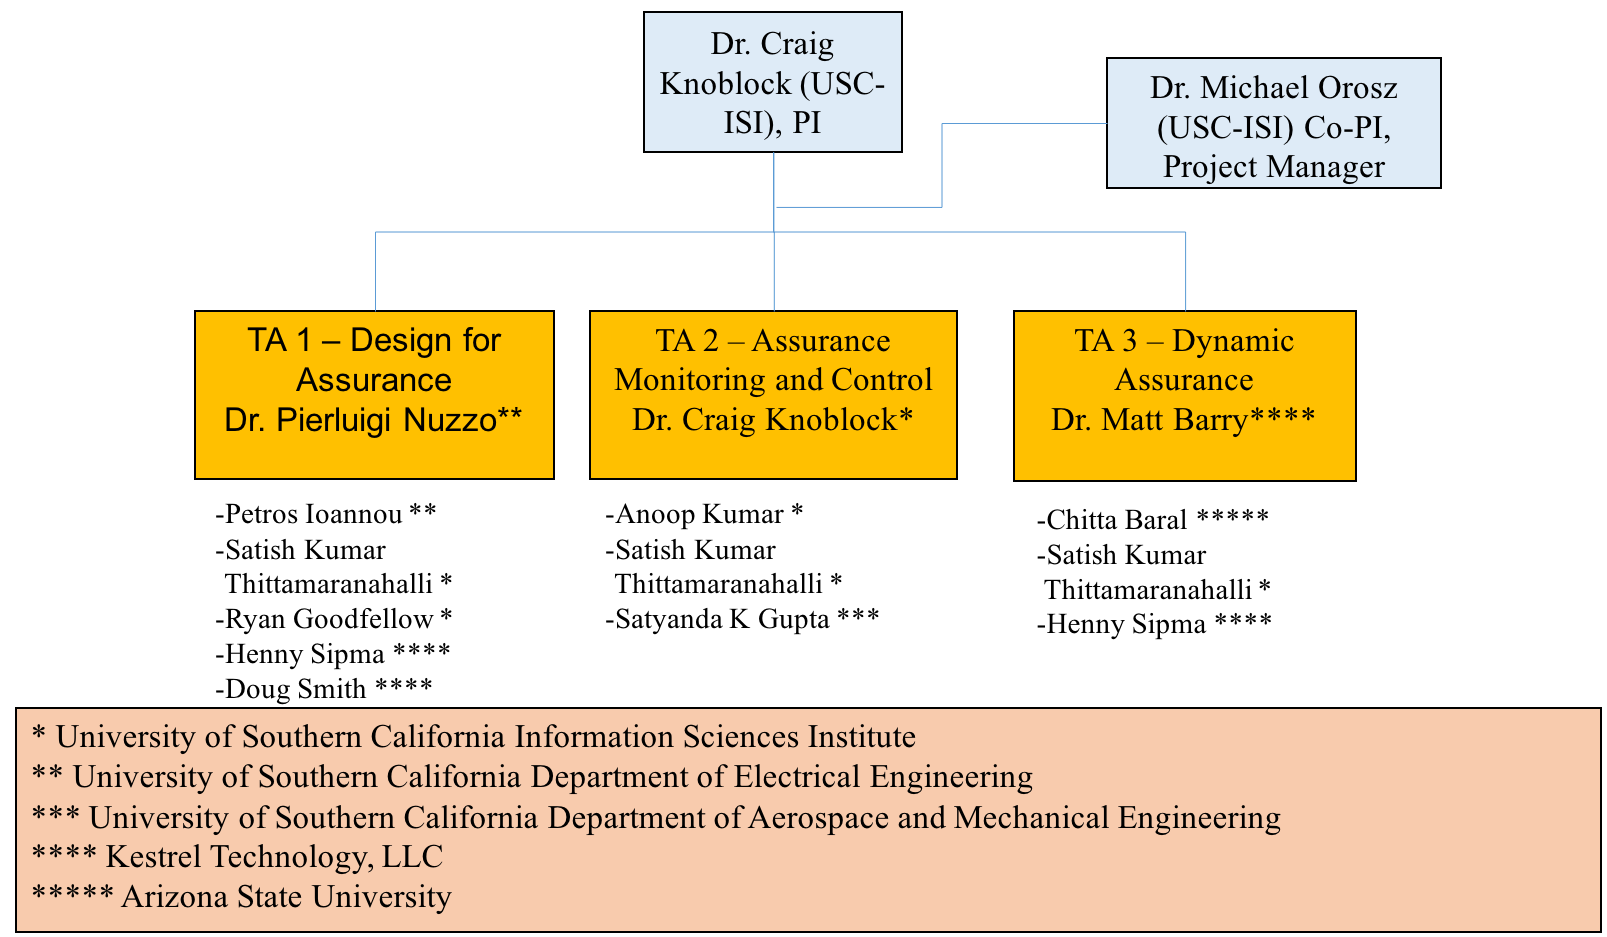
\includegraphics[width=6.0in]{./org-chart2.png}
\caption{\small Organization Chart}
\label{fig:org_chart}
\end{figure}

Coordination: To maximize collaboration and reduce risk to project failure from lack of communication and technical exchange, we plan to employ a wide variety of working styles and communication/coordination so that all can contribute.  At the core of our project will be regularly scheduled meetings bridging the diversely distributed team (Table~\ref{fig:Collaboration_Table}).  These meetings will address project status, identify challenges, implement risk mitigation strategies and participate in technology exchanges and system integration efforts (when appropriate)

\begin{table}[ht]
\caption{\small Project Meetings and Events}
  \centering
  {\footnotesize
\begin{tabular}{|m{3.15in}|m{3in}|} 
\hline
\textbf{Meeting} & \textbf{Frequency} 
\\\hline
Conference calls among investigators (discuss project status, address concerns and project risks) & Weekly
\\
\hline
Technical exchange and coordination meetings using Bluejeans or another videoconference technology & At least twice a month and more frequently as needed
  \\ 
\hline
Face-to-Face meetings (prior to P/I and demonstration meetings) & Every 3 to 6 months and more frequently (especially at the beginning of the project) as needed
 \\\cline{1-2}

\hline
\end{tabular}
}
\label{fig:Collaboration_Table}
\end{table}

\begin{table}[tbhp]
\caption{\small Key Project Team Member Responsibilities}
  \centering
  {\footnotesize
\begin{tabular}{| m{.75in} | m{3.9in}| m{1.5in}|} 
\hline
\textbf{Key Member} & \textbf{Responsibilities} & \textbf{Tasks} 
\\\hline
Dr.\ Craig Knoblock  & Principal Investigator responsible for project, leads TA 2 – Assurance Monitoring and Control.  Will lead the overall project and lead the TA2 team.  Served as the PI on many DARPA projects and has sucessfully led many large teams.    Effort on project:  25\% &
1.1.6, 1.2.2 1.2.3, 1.2.4, 1.3.4, 1.4.1, 
2.1.6, 2.2.2 2.2.3, 2.2.4, 2.3.4, 2.4.1, 
3.1.6, 3.2.2, 3.2.3, 3.2.4, 3.3.4, 3.4.1
\\
\hline
Dr.\ Michael Orosz & Co-Principal Investigator responsible managing the day-to-day operations of the project, assist technical teams as needed, coordinate with TA4 teams.    Has led many large complex multi-disciplined/multi-organizational projects in academic and industry environments.  Effort on project: 50\%
& 1.1.6, 2.1.6, 3.1.6, 1.4.1, 2.4.1, 3.4.1
  \\ 
\hline
Dr.\ Pierluigi Nuzzo 
& 
Co-Principal Investigator.  Leads the TA 1 - Design for Assurance team and conducts research on the formal methods for the design of the TA1 system.  Research experience on methodologies and tools for the design of cyber-physical systems; contracts, interfaces, and compositional methods for embedded system design; the application of automated formal methods and optimization theory to problems in embedded and cyber-physical systems.  Effort on project: 2 months/year (16.6\%)
& 
1.1.1, 2.1.1, 3.1.1 \\
\hline
Dr.\ Matthew Barry
& 
Key personnel.  Leads the TA 3 – Dynamic Assurance.   He will conduct the research on the dynamic assurance case language editors and parsers, the run-time system, and system integrations. Effort on project:  66\%
& 
1.3.2, 2.3.2, 3.3.2\\
\hline
Dr.\ Chitta Baral
& 
Key personnel responsible for learning assurance rules, supporting assurance rules with uncertainty and improving solver speed.  Expertise on ASP solvers, which will be used to reason about the assurance cases. Effort on project: 20\%
& 
1.3.1, 2.3.1, 3.3.1 \\
\hline
Dr.\ Doug Smith 
& 
Key personnel will support formal methods aspects of TA1, and lead the effort on abstract refinement. Expertise in field of automated correct-by-construction program generation.    Effort on project: 40\%
& 
1.1.5, 2.1.5, 3.1.5 \\
\hline
Dr.\ Henny Sipma
& 
Key personnel who will support the program verification tasks under TA1.  Will lead the effort on program verification.   Effort on project:  45\%
& 
1.1.5, 2.1.5, 3.1.5, 1.3.2, 2.3.2, 3.3.2 \\
\hline
Dr.\ Petros Ioannou
& 
Key personnel responsible providing and extending the assurance test bed, which will be available at the start of the project for autonomous vehicles.   Effort on project: 1 month/year (8.3\%)
& 
1.1.2, 2.1.2 (optional), 3.1.2 (optional)
\\
\hline
Dr.\ Satyandra Kumar Gupta
& 
Key Personnel providing autonomous command and control expertise to the TA-2 team.   Will lead the research on safety aware learning on TA2.   Past research on physics-aware decision making to facilitate automation.  Effort on project: 1 month/year (8.3\%)
& 
1.2.1, 2.2.1, 3.2.1 \\
\hline
Dr.\ Anoop Kumar 
& 
Key personnel providing support to the TA 2 project team.  Will lead the research on monitoring \& control and detecting distribution shifts.  Effort on project: 50\%
& 
1.2.1, 1.2.2, 1.2.3, 1.2.4, 2.2.1, 2.2.2, 2.2.3, 2.2.4, 3.2.1, 3.2.2, 3.2.3, 3.2.4\\
\hline
Dr.\ Satish Thittamaranahalli
& 
Key personnel developing scalable algorithms for TA1, TA2, and TA3 project teams.  Has extensive experience on scalable algorithm design, machine learning, and constraint reasoning.  Effort on project: 50\%
& 
1.2.1, 1.2.2, 1.2.3, 1.2.4, 2.2.1, 2.2.2, 2.2.3, 2.2.4, 3.2.1, 3.2.2, 3.2.3, 3.2.4, 1.1.4, 2.1.4, 3.1.4 \\
\hline
Dr.\ Ryan Goodfellow
& 
Key personnel providing support to the TA-1 project. Will lead the research on simulation-based testing.  Has extensive experience on simulation-based testing.  Effort on project:  30\%
& 
1.1.3, 2.1.3, 3.1.3 \\

\cline{1-2}

\hline
\end{tabular}
}
\label{fig:Table_Mgmt}
\end{table}



\newpage
\section{Personnel, Qualifications and Commitment}

{\bf Dr.\ Craig Knoblock}, the PI on this effort, is a Research Professor of both Computer Science and Spatial Sciences at the University of Southern California (USC) and Director of the Intelligent Systems Division at the USC Information Sciences Institute.   He received his Ph.D. from Carnegie Mellon University in computer science. 
%His research focuses on techniques for describing, acquiring, and exploiting the semantics of data.  
In previous projects he has worked on developing  scalable approaches to execution monitoring, accurate detection of sensor failures, and   automatic modeling and reconstruction of sensors.  He has published more than 300 journal articles, book chapters, and conference papers on these topics.  Dr. Knoblock is a Fellow of the Association for the Advancement of Artificial Intelligence (AAAI), a Distinguished Scientist of the Association of Computing Machinery (ACM), a Senior Member of IEEE, past President and Trustee of the International Joint Conference on Artificial Intelligence.
%and winner of the 2014 Robert S. Engelmore Award.  

{\bf Dr.\ Michael Orosz}, a Co-PI on this effort, is a Research Associate Professor of Civil and Environmental Engineering at the University of Southern California (USC) and Research Director of the Decision Systems Group at the USC Information Sciences Institute.  Dr. Orosz has over 30 years’ experience in commercial and government software development, basic and applied research, project management, academic research and has developed and deployed several commercially successful products.  His research interests are in machine learning and decision analytics as applied to intelligence analysis and autonomous command and control such as smart building controls.    Dr. Orosz has extensive experience in managing large complex multi-disciplined/multi-teamed research projects. %funded by DARPA, DHS, DoD, DoE, Industry, NASA, NRO, NSA and ONR.   
He received his Ph.D. in computer science from the University of California, Los Angeles.

{\bf Dr.\ Pierluigi Nuzzo}, a Co-PI on this project, is an Assistant Professor in the Department of Electrical Engineering at the University of Southern California. He received the Ph.D. in Electrical Engineering and Computer Sciences from the University of California at Berkeley. 
%in 2015, and the Laurea degree (MS) in electrical engineering (summa cum laude) from the University of Pisa, Italy, and the Sant'Anna School of Advanced Studies, Pisa, Italy.
%
%He has four years of research experience in analog and mixed signal circuit design as a researcher at IMEC, Leuven, Belgium, and over 10 years experience in design methodologies and tools for mixed-signal integrated circuits and cyber-physical systems, as a researcher at the University of Pisa, IMEC, UC Berkeley, and USC. 
His research interests
include: methodologies and tools for cyber-physical system and mixed-signal
system design; contracts, interfaces and compositional methods for embedded
system design; the application of formal methods and optimization theory to problems in embedded and cyber-physical systems and electronic design automation. 
%
Prof. Nuzzo received %First Place in the operational category and Best Overall
%Submission in the 2006 DAC/ISSCC Design Competition, 
a Marie Curie Fellowship
from the European Union in 2006, 
the University of California at Berkeley EECS
departmental fellowship in 2008, 
%the University of California at Berkeley Outstanding Graduate Student Instructor Award in 2013, 
the IBM Ph.D.
Fellowship in 2012 and 2014, 
%the Best Paper Award from the International Conference on Cyber-Physical Systems (ICCPS) in 2016, 
and the David J.~Sakrison Memorial Prize in 2016 for his doctoral research. 
%He is an author of 1 patent and over 60 publications.

{\bf Dr.\ Satyandra K. Gupta} is Smith International Professor in the Department of Aerospace and Mechanical Engineering at the University of Southern California. %Prior to joining the University of Southern California, he was a Professor in the Department of Mechanical Engineering and the Institute for Systems Research at the University of Maryland. He was the founding director of the Maryland Robotics Center and the Advanced Manufacturing Laboratory at the University of Maryland. 
He served as a program director for the National Robotics Initiative at the National Science Foundation from September 2012 to September 2014.  Dr. Gupta's interest is in the area of physics-aware decision making to facilitate automation. He has published more than 300 technical articles. He is a fellow of the American Society of Mechanical Engineers (ASME) and editor of ASME Journal of Computing and Information Science in Engineering. Dr. Gupta has received the Young Investigator Award from the Office of Naval Research in 2000, CAREER Award from the National Science Foundation in 2001, Presidential Early Career Award for Scientists and Engineers (PECASE) in 2001, Invention of the Year Award at the University of Maryland in 2007, Kos Ishii-Toshiba Award from ASME in 2011, and Excellence in Research Award from ASME in 2013.%, and Distinguished Alumnus Award from Indian Institute of Technology, Roorkee in 2014. %He has also received seven best paper awards at conferences.

{\bf Ryan Goodfellow} is a computer scientist at ISI working in combined cyber physical simulation and emulation platform development. His formal background is in simulation algorithms and modeling techniques using differential-algebraic equations (DAE). He has applied this knowledge in the CPS space by integrating DAE modeling languages and simulation engines with network testbeds to create comprehensive scientific experimentation platforms for cyber-physical systems. These experimentation platforms have been used in the power grid research space. %Ryan is a lead developer on the Deter network testbed, with a strong background in networked and distributed systems engineering. %He is also a combat veteran, serving as a non-commissioned officer and SIGINT team lead for a multi-functional intelligence team in Afghanistan.

{\bf Dr.\ Petros Ioannou} is a Professor in the Department of Electrical Engineering, Director of the Center for Advanced Transportation Technologies and Associate Director for Research for the DOT supported University Transportation Center at USC. He received his MS and PhD from the University of Illinois at Urbana Champaign in Mechanical and Electrical Engineering, respectively. His research interests are in robust adaptive control, vehicle dynamics and control, human factors and safety, automated vehicles, nonlinear systems and Intelligent transportation Systems.  He received the 2016 IEEE Transportation Technologies field award and the 2016 IEEE Control system society Transition to Practice Award. He is a Fellow of IEEE, IFAC and IET and author/coauthor of 8 books and over 400 papers.

{\bf Dr.\ Matthew Barry} will serve as lead for the TA3 tasks. %He will implement the dynamic assurance case language editors and parsers, the run-time system, and system integrations.  He will implement the assurance case arguments and the API for updating argument structure and content.  
Dr. Barry currently is CEO at Kestrel Technology LLC, and previously spent 20 years in NASA space mission operations at the Jet Propulsion Lab and Johnson Space Center.  At NASA Headquarters he led the introduction of dependability case requirements and plans for flight computing systems in upcoming manned space exploration missions, as well as the development of Agency-level software-related safety-critical control system requirements.  He recently served as a Principal Investigator on DHS/Cyber S\&T STAMP (Static Tool Analysis Modernization Program), DARPA CSFV (Crowd Sourced Formal Verification), three NASA Aeronautics R\&D projects, and the AFRL-sponsored Static Analysis of Numerical Algorithms project.  Dr. Barry earned BSME, MS, and PhD degrees in mechanical engineering, and an MBA degree, from Rice University.  

{\bf Dr.\ Henny Sipma} will support the program verification tasks under TA1.  %She is the key person behind the company's {\em KT Advance\/} and {\em KT Transferal\/} static analysis products, and the designer and programmer of the company's core {\em CodeHawk\/} abstract interpretation engine. 
Dr. Sipma currently is the CTO at Kestrel Technology LLC.  She has spent the past 10 years with Kestrel Technology as a static analysis expert; previously developed and taught static analysis techniques as senior research associate at Stanford University for eight years; and developed industrial process controls as an senior systems analyst at Shell.  She has been Principal Investigator or company lead on several recent R\&D projects for Federal agencies, including two projects under the IARPA STONESOUP (Securely Taking On New Executable Software of Uncertain Provenance) program; the DHS Cyber S\&T Gold Standard project; and the DARPA-sponsored STAC (Space-Time Analysis for Cybersecurity) and MUSE (Mining and Understanding Software Enclaves) programs.  Dr. Sipma earned 
%a BS degree in chemistry and an MS degree in chemical engineering at the University of Groningen in The Netherlands, and 
MS and PhD degrees in computer science from Stanford University.  

{\bf Dr.\ Douglas R.\ Smith} will support formal methods aspects of TA1, including the enforcement of safety properties and the generation of monitors.  He is President of Kestrel Technology LLC and Principal Scientist at Kestrel Institute.  He is a Fellow of the American Association of Artificial Intelligence (AAAI) and an ASE Fellow (Automated Software Engineering).  From 1986 to 2000, he taught an advanced graduate course on correct-by-construction software development at Stanford.  
%Dr. Smith has led the development of a series of software synthesis systems, including KIDS (Kestrel Interactive Development System), Specware, Designware, and Planware. 
%Applications domains have included a variety of complex high-performance planners and schedulers for the US Air Force.  He leads current projects on the generation of air mission plans and cyberoperations.  
Other recent projects focused on automated policy enforcement \cite{SmithD0703,SmithD08}, synthesis of secure network protocol codes, and the synthesis of high-performance constraint-solvers\cite{SmithD08c,SmithD13}.  Dr. Smith has over 30 years experience in the field of automated correct-by-construction program generation and has published over 100 papers. He has one patent.  He received the Ph.D. in Computer Science from Duke University% in 1979.  

{\bf Dr. Chitta Baral} is a Professor in the Department of Computer Science and Engineering at Arizona State University. He will support the TA3 efforts on Learning assurance rules, supporting assurance rules with uncertainty and improving solver speed. Dr. Baral has expertise in various aspects of autonomy and Artificial Intelligence. 
He wrote the first book on answer set programming (published by Cambridge University Press) the formal language behind our assurance rules. Some of his other works relevant to this proposal are: goal specification for autonomous systems, automatic construction of control rules for autonomous systems that satisfy given goals, combining machine learning with reasoning in various contexts, including image understanding. %He is the President of KR Inc. He is an associate editor of AIJ and has been an associate editor of JAIR.

{\bf Dr.\ Satish Kumar Thittamaranahalli (T. K. Satish Kumar)} leads the Collaboratory for Algorithmic Techniques and Artificial Intelligence (CATAI) at USC's Information Sciences Institute. He has published over 60 papers on numerous topics in Artificial Intelligence spanning such diverse areas as Constraint Reasoning, Planning and Scheduling, Probabilistic Reasoning, Robotics, Combinatorial Optimization, Approximation and Randomization, Heuristic Search, Model-Based Reasoning, Knowledge Representation and Spatio-Temporal Reasoning. %He %has served on the Program Committees of many international conferences in Artificial Intelligence
He and is a winner of the 2016 Best Robotics Paper Award and the 2005 Best Student Paper Award from the International Conference on Automated Planning and Scheduling. 
Dr. Kumar received his PhD in Computer Science from Stanford University. %In the past, he has also been a Visiting Student at the NASA Ames Research Center, a Postdoctoral Research Scholar at the University of California, Berkeley, a Research Scientist at the Institute for Human and Machine Cognition, a Visiting Assistant Professor at the University of West Florida, and a Senior Research and Development Scientist at Mission Critical Technologies.

\textbf{Dr.\ Anoop Kumar} is a senior computer scientist at USC ISI and has broad expertise in machine learning, statistical modeling, and software engineering.  Dr.\ Kumar is the technical lead on the DARPA RSPACE program and has played a vital role in developing a system that fuses air operations data from multiple sources, maintains world state, and issues warnings. Previously, he led the research and development of the BBN’s election forecasting system for the IARPA OSI program. %Dr.\ Kumar played a significant role in the DARPA DEFT program by developing a model to support integration of output from multiple NLP algorithms. He has contributed at the development to management levels on government research contracts and commercial projects. 
Dr.\ Kumar helped design and develop BBN's commercially available, hosted speech and medical transcription services offering. 

\begin{table}[!tbh]
\begin{footnotesize}
\vspace{-0.1in}

\begin{tabular}{lll}
\begin{tabular}[t]{|l|@{}c@{}|@{}c@{}|@{}c@{}|@{}c@{}|} \hline
Project & Status & \multicolumn{3}{ c| }{Hours} \\ \cline{3-5}
& & P1 & P2 & P3 \\ \hline



\multicolumn{5}{ |c| }{ \textbf{Craig Knoblock} } \\ \cline{1-5}
Safeguard & Pro & 770 & 641 & 641 \\ \cline{1-5}
ELICIT & Cur & 308 & 256 & 120 \\ \cline{1-5}
WTNIC & Cur & 11 & 0 & 0 \\ \cline{1-5}
EFFECT & Cur & 641 & 107 & 0 \\ \cline{1-5}
LinkedMaps & Cur & 203 & 25 & 0 \\ \cline{1-5}
PRINCESS & Cur & 608 & 96 & 0 \\ \cline{1-5}
SCHARP & Cur & 481 & 54 & 0 \\ \cline{1-5}
MINT & Pen & 650 & 534 & 285 \\ \cline{1-5}

\multicolumn{5}{ |c| }{ \textbf{Michael Orosz} } \\ \cline{1-5}
Safeguard & Pro & 1560 & 1300 & 1300  \\ \cline{1-5}
SMC/SY & Cur & 1803 & 0 & 0  \\ \cline{1-5}

\multicolumn{5}{ |c| }{ \textbf{Matthew Barry} } \\ \cline{1-5}
Safeguard & Pro & 2078 & 1690 & 1554 \\ \cline{1-5}
Starlite & Cur & 1840 & 1692 & 0 \\ \cline{1-5}



\multicolumn{5}{ |c| }{ \textbf{Anoop Kumar} } \\ \cline{1-5}
Safeguard & Pro & 1560 & 1300 & 1300 \\ \cline{1-5}

\end{tabular}
&
\begin{tabular}[t]{|l|@{}c@{}|@{}c@{}|@{}c@{}|@{}c@{}|} \hline
Project & Status & \multicolumn{3}{ c| }{Hours} \\ \cline{3-5}
& & P1 & P2 & P3 \\ \hline

\multicolumn{5}{ |c| }{ \textbf{Pierluigi Nuzzo} } \\ \cline{1-5}
Safeguard & Pro & 520 & 433 & 433  \\ \cline{1-5}
Mirage & Cur & 433 & 0 & 0  \\ \cline{1-5}

\multicolumn{5}{ |c| }{ \textbf{Satyandra Gupta} } \\ \cline{1-5}
Safeguard & Pro & 260 & 217 & 217 \\ \cline{1-5}
Human   & Cur & 22 & 0 & 0 \\ \cline{1-5}
Vehicles & Cur & 36 & 0 & 0 \\ \cline{1-5}
Robot & Cur & 116 & 0 & 0 \\ \cline{1-5}
Assembly & Cur & 33 & 0 & 0 \\ \cline{1-5}
Solar & Cur & 4 & 0 & 0 \\ \cline{1-5}

\multicolumn{5}{ |c| }{ \textbf{Petros Ioannou} } \\ \cline{1-5}
Safeguard & Pro & 260 & 217 & 217 \\ \cline{1-5}
CPS & Cur & 130 & 0 & 0 \\ \cline{1-5}

\multicolumn{5}{ |c| }{ \textbf{Ryan Goodfellow} } \\ \cline{1-5}
Safeguard & Pro & 936 & 780 & 780 \\ \cline{1-5}
STEAM & Cur & 416 & 0 & 0 \\ \cline{1-5}


\end{tabular}
&
\begin{tabular}[t]{|l|@{}c@{}|@{}c@{}|@{}c@{}|@{}c@{}|} \hline
Project & Status & \multicolumn{3}{ c| }{Hours} \\ \cline{3-5}
& & P1 & P2 & P3 \\ \hline

\multicolumn{5}{ |c| }{ \textbf{Chitta Baral} } \\ \cline{1-5}
Safeguard & Pro & 659 & 485 & 485 \\ \cline{1-5}
PostdocBP & Cur & 176 & 0 & 0 \\ \cline{1-5}
Languages & Pen & 528 & 264 & 264 \\ \cline{1-5}
CAREER & Pen & 88 & 44 & 44 \\ \cline{1-5}
CHS & Pen & 510 & 255 & 0 \\ \cline{1-5}

\multicolumn{5}{ |c| }{ \textbf{Doug Smith} } \\ \cline{1-5}
Safeguard & Pro & 1222 & 984 & 840 \\ \cline{1-5}
RSPACE & Cur & 342 & 0 & 0 \\ 
\cline{1-5}
PLANX & Cur & 154 & 0 & 0 \\ 
\cline{1-5}
HACCS & Pen & 923 & 769 & 769 \\ 
\cline{1-5}

\multicolumn{5}{ |c| }{ \textbf{Henny Sipma} } \\ \cline{1-5}
Safeguard & Pro & 1372 & 962 & 840 \\ \cline{1-5}
STAC & Cur & 797 & 0 & 0 \\ \cline{1-5}

\multicolumn{5}{ |c| }{ \textbf{Satish Thittamaranahalli} } \\ \cline{1-5}
Safeguard & Pro & 1560 & 1300 & 1300 \\ \cline{1-5}
MapF & Cur & 103 & 103 & 0 \\ \cline{1-5}

\end{tabular}
\end{tabular}

\end{footnotesize}
\caption{Individual commitments of key personnel}
\label{tab:Commitments}
\vspace{-0.2in}
\end{table}

\clearpage
\newpage
\section{Capabilities}


%\subsection{University of Southern California}
USC has strengths in number of areas that are closely related to the proposed work:
\begin{itemize}[itemsep=0pt,leftmargin=*]
\item Dr.\ Nuzzo 
%has over 10-year research experience in embedded system design, from mixed-signal chip design (analog-to-digital converters, frequency synthesizers, software-defined radio), to methodologies and tools for mixed-signal integrated circuits and Cyber-Physical Systems (CPSs), and the application of formal methods and optimization theory to problems in embedded and cyber-physical systems and electronic design automation.  
%His doctoral work 
has done extensive research on contracts and compositional methods for heterogeneous system design and design space exploration, with application to aircraft electric power systems and environmental control systems. His work has helped transition rigorous system design foundations, innovative design methodologies, and new systems engineering paradigms to industry (IBM, United Technologies). 
\item Dr.\ Satyandra K. Gupta has worked on autonomous surface vehicles, autonomous ground vehicles for operation on rugged terrains, and autonomous flapping wing aerial vehicles.   His group has developed a hierarchal decision making approach for realizing autonomous systems. 
%This approach combines task planning and assignment, deliberative trajectory planning, reactive collision avoidance behaviors, and trajectory tracking control layers. 
His group has also developed new methods for learning reactive behaviors in adversarial environments and COLREGS compliant trajectory planning. \item Dr.\ Knoblock has developed methods that learn the relationships between sensors to both identify failures and changes in sensor and reconstruct those sensors, providing estimates of the accuracy of the reconstructed sensors.  
\item Ryan Goodfellow has extensive experience in simulation based testing through high-fidelity CPS testbed environment development and operation, using the Deter network testbed as the core which has supported several large scale government projects from a variety of agencies and thousands of users. %we have developed sophisticated CPS experiments under programs such as NFS RIPS, NIST SmartCities and the DHS Cybersecurity showcase.
\item Dr.\ Ioannou %helped  design and implement adaptive cruise control systems in collaboration with Ford Motor Company, which was commercialized four years before any other company. He 
worked on several DOT funded projects on automated vehicles and intelligent highway systems where he demonstrated his vehicle control designs for safety and performance on actual automated vehicles in test trucks and I-15 highway.
\item Drs.\ Knoblock, Kumar, and Thittamaranahalli have developed highly scalable approaches for monitoring message traffic to identify potential problems and issue warnings and alerts. 
\item Dr. Thittamaranahalli has developed state-of-the-art methods for efficiently solving large-scale search and optimization problems. %These techniques will be applicable in TA2 for safety-aware learning and planning, in TA2 for assurance monitoring and control, and in TA3 for dynamic assessment of assurance cases.

\end{itemize}
%\subsection{Kestrel Technology LLC}

Kestrel Technology's strength is in program analysis, specifically static analysis of both source and binary targets.  The company performs applied R\&D and product development for a variety of static analysis applications  pivoting primarily on the abstract interpretation technique.  The company recently initiated development of program analysis applications using logical equivalence techniques. As a provider of verification evidence in the form of mathematical proofs, the company also has expertise in the design and development of assurance case arguments for high-integrity systems using such evidence. %The company is engaged in a partnership with Wind River Systems to develop program analysis tools for its embedded system developers.  Many of Wind River's customers must develop their products under safety and certification standards, including those using safety cases.  

   

%\subsection{Arizona State University}
Chitta Baral at Arizona State University has developed various software to learn assurance rules and various ASP solvers, which he has made available as open-source.

Most of the software carried forward for implementation or derivation is open source.  The single exception is Kestrel Technology's {\it KT Advance\/} static analysis tool (TA1), in particular the abstract interpretation engine therein, which is company proprietary and is US EAR export-controlled.   
%Owing to mixed funding for the development of that technology 
We will continue to provide the Federal government a restricted use license for that particular item.

There are no specialized facilities, data, or GFE required for this effort. 

\include{sow}
\include{milestones}

% \section{Level of Effort by Task \textcolor{red}{[Mike/Lisa - 1 pages]}}

% \textcolor{blue}{
% \begin{itemize}
% \item Will be a separate spreadsheet
% \item
% \end{itemize}
% }

\include{appendix_a}

%\section{Appendix B \textcolor{red}{[No Page Count]}}

\section{References}
\bibliographystyle{acm} 
\bibliography{TA3/ta3,TA2/ta2,TA1/ta1}
\end{document}
%%\documentclass[a4paper]{article}
%\documentclass[12pt]{article}
\documentclass[12pt]{dod-blank}

%% Language and font encodings
\usepackage[english]{babel}
\usepackage[utf8x]{inputenc}
\usepackage[T1]{fontenc}

%% Sets page size and margins
%%\usepackage[a4paper,top=3cm,bottom=2cm,left=3cm,right=3cm,marginparwidth=1.75cm]{geometry}
%\usepackage[top=1in, bottom=1in, left=1in, right=1in]{geometry}



%% Useful packages
\usepackage{amsmath}
\usepackage{graphicx}
  \graphicspath{{.}{./image/}}
  \DeclareGraphicsExtensions{.png,.jpg} 
\usepackage[colorinlistoftodos]{todonotes}
\usepackage[colorlinks=true, allcolors=blue]{hyperref}
\usepackage{tabularx}
\usepackage{multirow}
\usepackage{tabulary}
\usepackage{float}
\usepackage{wrapfig}
\usepackage[export]{adjustbox}
\usepackage{comment}
\usepackage{tabularx}
\usepackage{multirow}
\usepackage{tabulary}
\usepackage{enumitem}

\usepackage{listings}
\usepackage{color}
\usepackage{array}
\usepackage{subcaption}
\usepackage{xcolor}




\renewcommand{\textfraction}{0}
\renewcommand{\topfraction}{1.0}
\renewcommand{\bottomfraction}{1.0}

\usepackage{longtable}
%% macros
\newif\iffinal
\finaltrue
\iffinal
  
    \newcommand\baareq[1]{}
    \newcommand\baades[1]{}
 
 
\else
    \definecolor{darkgreen}{rgb}{0,0.4,0}
    \definecolor{darkcyan}{rgb}{0,0.4,0.4}
    \definecolor{darkblue}{rgb}{0,0,0.5}
    
    \newcommand\baareq[1]{{\color{darkcyan}[\textbf{Requirement:} #1]}}
    \newcommand\baades[1]{{\color{darkcyan}[\textbf{Description:} #1]}}
 
\fi




\def\naive{na\"{\i}ve}



\lstset{ 
  backgroundcolor=\color{white},   % choose the background color; you must add \usepackage{color} or \usepackage{xcolor}
  basicstyle=\footnotesize\ttfamily,            % the size of the fonts that are used for the code
  breakatwhitespace=false,         % sets if automatic breaks should only happen at whitespace
  breaklines=true,                 % sets automatic line breaking
  captionpos=b,                    % sets the caption-position to bottom
  commentstyle=\color{mygreen},    % comment style
  % deletekeywords={...},            % if you want to delete keywords from the given language
  escapeinside={\%*}{*)},          % if you want to add LaTeX within your code
  extendedchars=true,              % lets you use non-ASCII characters; for 8-bits encodings only, does not work with UTF-8
  frame=single,	                   % adds a frame around the code
  keepspaces=false,                 % keeps spaces in text, useful for keeping indentation of code (possibly needs columns=flexible)
  keywordstyle=\color{blue}\bfseries\underbar,       % keyword style
  language=Prolog,                 % the language of the code
  % morekeywords={if,and},        % if you want to add more keywords to the set
  numbers=none,                    % where to put the line-numbers; possible values are (none, left, right)
  numbersep=5pt,                   % how far the line-numbers are from the code
  numberstyle=\tiny\color{mygray}, % the style that is used for the line-numbers
  rulecolor=\color{black},         % if not set, the frame-color may be changed on line-breaks within not-black text
  showspaces=false,                % show spaces everywhere adding particular underscores; it overrides 'showstringspaces'
  showstringspaces=false,          % underline spaces within strings only
  showtabs=false,                  % show tabs within strings adding particular underscores
  stepnumber=2,                    % the step between two line-numbers. If it's 1, each line will be numbered
  stringstyle=\color{mymauve},     % string literal style
  tabsize=2,	                   % sets default tabsize to 2 spaces
  title=\lstname                   % show the filename of files included with \lstinputlisting; also try caption instead of title
}

% apply trick for additional keywords for our AC DSL
\lstset{
	emph={for, if, and, or},
    emphstyle={\color{blue}\bfseries\underbar}
}




\title{DARPA Assured Autonomy}
\author{Technical Volume- \textcolor{red}{Thirty-Eight (38) pages max}}

\begin{document}
\pagenumbering{roman}
\include{cover}

\newpage
\section{Table of Contents}
\tableofcontents

\newpage
\pagenumbering{arabic}
\section{Executive Summary}
As we rapidly move into a world where machine learning plays a central role in realizing autonomous systems, it is becoming increasingly important to develop techniques that assure that these systems will operate safely and perform as expected. Current approaches are limited to providing assurance for systems with limited or no  learning capabilities. In this context, DARPA's Assured Autonomy BAA seeks to \emph{develop rigorous design and analysis technologies for continual assurance of learning-enabled autonomous systems}. USC in collaboration with Kestrel Technology and ASU is pleased to submit a comprehensive TA1, TA2, and TA3 proposal entitled \emph{``Assured Autonomy for Learning Enabled Vehicles (Safeguard).''} We plan to provide an end-to-end solution to support autonomous systems with learning-enabled components, ranging from design technologies for assurance, to assurance monitoring and control techniques, to representation and online evaluation of assurance cases. We have assembled a strong team of experts that cover the range of technologies that are required to create such an end-to-end system. If successful, the project will provide the technologies for building the next-generation of learning-enabled autonomous systems.  The entire project will take four years and cost \textcolor{red}{\$??}, with an initial version completed at the end of Phase I and successive versions with additional capabilities and improved scalability at the end of Phase II and Phase III.  

In the remainder of this section, we first introduce an  unmanned surface vehicle scenario that will be used throughout the proposal to describe the approach.  Next, we describe our approach to design, monitoring, and dynamic assurance. Finally, we introduce the team involved in the project. 

\textbf{Motivating Scenario.} Consider an autonomous unmanned surface vehicle (USV) guarding a valuable asset in the ocean when an unknown vehicle  approaches the security perimeter, under challenging weather conditions. In this scenario, the USV is required to approach the intruding vehicle, issue a warning signal, and escort it to a safe distance from the controlled area. However, as the USV has no a priori knowledge of its external environment behaviors (e.g., water depth, waves, wind, current, visibility), pre-computing a feasible trajectory, let alone optimal, becomes a non-trivial problem. For trajectory planning, the USV must continuously perform the following tasks:
\begin{itemize}[itemsep=0pt,leftmargin=*]
 \item Sense the current state of the surrounding environment (e.g., water depth, waves, wind, current, visibility) and estimate its own maneuverability constraints (e.g., braking distance, available acceleration, maximum velocity, turning radius, turning rate, safety distance) based on the state of the environment;      
\item Sense the static obstacles in the sensor range and generate a traversability map;
\item Sense the moving obstacles and classify them;   
\item Predict future trajectories of moving obstacles; 
\item Determine if any of the COLREGS \cite{commandant1999international} rules will be in effect with respect to one or more of the nearby vessels and identify the vessels with the right of way.    
\end{itemize}
The above information will be used by the trajectory planner to compute an initial trajectory, which will be continuously refined as the USV gathers additional information.
% It is not possible for the USV to be tested in every possible environment. 
The USV will use learning enabled components to take  decisions as it encounters new situations, such as  
\begin{itemize}[itemsep=0pt,leftmargin=*]
\item Classifiers to identify moving obstacles based on physical appearance and motion signatures,
\item Algorithms to estimate the sensor capabilities in adverse weather conditions,   
\item Algorithms to accurately estimate uncertainty in the environment, 
\item Classifiers to generate traversability maps,
\item Prediction of external vessel behaviors based on motion histories, 
\item Reinforcement learning  to ensure COLREGS compliance of maneuvers,  
\item Algorithms to learning pursuit behaviors.  
\end{itemize}
Learning enabled components will interact with each other in complex ways, where a misclassification error in one component may eventually compromise the entire mission.   
% We will need to make sure that each learning enabled components has a run-time monitor that will ensure that the assumptions made by the learning-enabled component remain valid and prevent erroneous learning. 
% For example, if the vehicle is exhibiting significant error in trajectory tracking, then simply downgrading the trajectory tracking error value may not be a good option.  The failure of prediction of trajectory tracking error might be due to the presence of a significant wake caused by a nearby vessel. The presence of the nearby vessel can be used to explain the degradation in trajectory tracking performance. As the vessel moves away, we can expect the trajectory tracking performance to return to the predicted level.  
While exhaustive validation of learning-enabled cyber-physical systems (LE-CPSs) is a prohibitive task~\cite{Kalra16},
their complexity, heterogeneity, and highly dynamic nature
make it challenging to even leverage existing model-based development techniques to effectively assess system correctness 
% dependability, 
at design time or enforce it at runtime.

\textbf{Design for Assurance.} Safeguard uses a platform-based design approach~\cite{Nuzzo15b} to organize the design process for a LE-CPS and to build assurance cases. Composite models are developed at several levels of abstraction,
from top-level system requirements and safety constraints down to the
implementation level.  Intermediate levels add detail to the levels
above.  The different levels are connected by refinement mappings that
allow properties established at one level to be preserved at the next
level (see Figures~\ref{fig:methodology} and~\ref{fig:assurance}).

Contracts are used to formally specify components and composite models
in terms of (1) Assumptions -- the assumed behaviors of the
environment and the behaviors of other components, and (2) Guarantees
-- the behavior properties that a model guarantees if it operates in a
context that satisfies its assumptions.  A calculus of contracts
allows horizontal composition of contracts to generate contracts for
composite models.  Vertical contracts are used to specify the mapping
or refinement relation between models at different levels of
abstraction.  The system design process starts with a high-level
contract that expresses overall system assumptions and requirements.
Subsequent levels express models with increasing detail until the
lowest level expresses the system in terms of hardware components and
their software controllers.

The assurance case for a CPS arises from the horizontal and vertical
structure of the design in several ways.  The components used within a
particular level are either (1) synthesized using
correct-by-construction design tools together with proofs, (2) derived
statically or dynamically using safety-aware machine-learning
techniques, (3) written manually and verified by analysis tools, or
(4) written manually and validated by extensive testing.  The
assurance case for the whole reflects its compositional structure.  We
anticipate that well-specified contracts together with the calculus of
contracts will eliminate well-known problems with unexpected emergent
behaviors in CPS systems.

The assurance case for the lowest-layer design arises from both the
intra-level assurance and from properties and their proofs that are
preserved under the refinement mapping from the top-level
requirements.  The refinement mappings between model layers will be
constructed using a variety of techniques.  A contract at an abstract
level can be mapped to a component or refined contract by (1)
retrieval of pre-verified components from a platform library, (2)
synthesis using correct-by-construction design and optimization tools,
or (3) manual coding to satisfy a contract.  The mapping of a
composite model will be composed from the mappings of its constituent
components or contracts.  When a composite model cannot be mapped
compositionally to the next level, it will be generated using
correct-by-construction design and optimization tools.

\textbf{Assurance Monitoring and Control.}
We provide an integrated framework for safety-aware learning, assurance monitoring and control, detecting distribution shifts. Three major components offer an efficient TA2 architecture as well as interfaces with TA1 and TA3, that is, (a) safety-aware learning and planning, (b) assurance monitors for guarding architectural and safety constraints; and (c) distribution shift detection.

We will develop a new learning-enabled online decision-making framework that allows opportunistically composing a sequence of actions (maneuvers) to reduce uncertainty in the system capability model without suspending the progress toward the mission goals or compromising safety. Each candidate action is evaluated based on three criteria: (1) the risk of violating a safety constraint using the current uncertainties in the parameter estimates; (2) its relevance to the mission goals; (3)  its expected information gain, i.e., reduction in uncertainty, with respect to the parameter estimates. These evaluations are combined to produce a cumulative mission utility value for each action that drives our learning-enabled decision-making framework. The problem of generating and evaluating sequences of actions can be posed in several way. For example, it can be solved using a branch-and-bound search method like Anytime A*, or formulated with the finite-horizon Markov Decision Process (MDP) framework. We will develop new scalable search strategies to solve this problem efficiently, by potentially evaluating a recent method developed at USC, called FastMap, that can significantly improve the execution time. 

We will develop monitors for architectural and safety constraints. 
% While these constraints can be checked over and over again as sensor information flow in, this naive strategy accounts for a lot of computational overhead. 
To achieve scalability and decrease the overhead, we propose the application of a technique that we currently use in DARPA's RSPACE program, which leverages a physical model of the vehicles dynamics and its interactions with the environment to efficiently determine the readout frequency. We propose two  extensions of this basic idea. First, we will use the theory of Variable Elimination to prioritize which variables to monitor, e.g., controllable, versus uncontrollable, adversarially controlled, or unobservable variables. Second, we invoke the dynamic assessment of assurance cases only when needed. This  decreases the number of times dynamic assessment of assurance cases is initiated as well as the communication bandwidth between the TA2 and TA3 components.

Finally, we will identify a distribution shift by combining statistical and machine learning techniques to differentiate between environmental and sensor changes. We will exploit a categorization of the shifts based on their cause and duration as well as extend our earlier work on detecting and mitigating sensor failures for all types of monitored variables.  

\textbf{Dynamic Assurance:} The Safeguard {\em design for assurance\/} activity takes a systems-theoretic stance toward safety.  Consequently, it presumes that safety is an emergent property of the system, and that hazards can present themselves through unintended interactions and performance violations in addition to causal events such as component failures.  Our design approach includes consideration of intent as well as hazard analysis and mitigation.  The artifacts from these activities populate contracts and assumptions for the dynamic assurance case.  
We thus build safety into the product by working at a systems-level viewpoint, using lexicon and design patterns familiar to both hardware and software engineers; safety is an emergent property of the system, not an afterthought.  
As system behavior evolves during runtime owing to learning, threats, degradation, or some other factor, the dynamic assurance case identifies whether the safety constraints continue to be satisfied.  If not, it provides notifications or issues recovery instructions directly from a lookup table.

Our implementation of the dynamic assurance case employs a declarative knowledge base inference engine and a domain-specific language tailored to our approach.  We have used them successfully for assurance case tool sets and arguments, and will extend them to reason about uncertainty and learning.  Our approach to achieve scalability is to specialize solvers toward modularity and to take advantage of domain knowledge.  Specifically, we will develop answer set programming techniques for context-dependent learning for reasoning about the learning-enabled components as well as learning assurance rules.  We will develop new formalisms for uncertainty to include causality, using weights for computing probabilities, and probabilistic non-monotonicity.  To achieve scaling objectives we will implement specializations using modularity, weighted CSPs, and message passing. 

% The system safety constraints revealed from that design become the key elements of our dynamic assurance case.  Our verification tools ensure the constraints are relevant, identifiable, and their implementation and effect observable.  

\textbf{Team.} We have assembled a team that is exceptionally well-qualified to build the proposed Safeguard system.  The team will be led by Dr.\ Craig Knoblock, the Principal Investigator for the effort, who currently leads the Intelligent Systems Division at the Information Sciences Institute.  He has led many large DARPA and IARPA projects over the years and has a strong track record in conducting leading edge research and then transitioning the technology to commercial use.  He will be supported by Dr.\ Michael Orosz as the Project Manager, who also has  experience in managing large research projects and on autonomous systems.  The TA1 team will be led by Dr.\ Pierluigi Nuzzo, who is an expert in embedded system design methodologies and the  application of formal methods to cyber-physical systems.  The TA1 team also includes Dr.\ Doug Smith, who has spent many years working on scalable correct-by-construction techniques and Dr.\ Henny Sipma, who has significant experience in applying program verification methods to real-world problems.  The TA1 team also includes Ryan Goodfellow, who has done a large amount of work on simulation-based testing.  The TA2 team will be led by Dr.\ Knoblock who has worked on topics related to both monitoring and detecting distribution changes.  He will be supported by Dr.\ Satyandra Gupta, who is an expert on autonomous surface vehicles as well as on safety-aware learning. He will also be supported by Drs.\ Anoop Kumar and Satish Thittamaranahalli, who have also previously worked on efficient methods for execution monitoring.  The TA3 team will be lead by Dr.\ Matthew Barry, who has experience in creating the technologies for assurance cases.  He will be supported by Dr.\ Chitta Baral, who is an expert on ASP solvers and by Dr.\ Thittamaranahalli who is an expert on SAT solvers, both of which will be applied to provide scalable assurance case reasoning.  Finally, Dr.\ Petros Ioannou, who is an expert on control systems for autonomous vehicles will provide an autonomous vehicle platform, which will form the focus of our work until the TA4 teams provide additional vehicle platforms for development.  

\newpage
\section{Innovative Claims and Deliverables}

In this project we will develop and build an end-to-end system for assured autonomy.  This section describes the key innovations by technical area and then the overall deliverables of the project.

\paragraph{Design for Assurance}

\begin{itemize}[itemsep=0pt,leftmargin=*]
\item We address the LE-CPS design challenges via a holistic approach that can contextually generate design artifacts and assurance cases. We develop a compositional, contract-based modeling framework, methods, and tools to support the design process from system-level requirement capture,  formalization, and analysis, to the generation, testing, and continual monitoring of software and hardware artifacts in feedback loop with a physical process.

\item We develop compositional abstractions and interfaces (vertical contracts) that can  bridge heterogeneous formalisms and heterogeneous decomposition architectures to make system analysis and synthesis tractable, consistently combine different verification and synthesis methods at design time, and provide seamless support for dynamic assurance at run time. %We aim to quantitatively capture the confidence in the satisfaction of requirements under uncertain or unknown conditions, and resilience properties of  systems at different abstraction levels, to enable trade-off evaluation between resilience, performance, and cost.

\item We develop a unifying framework and efficient algorithms to reason about the combination of discrete and continuous dynamics and constraints in the presence of uncertainties in LE-CPS using a satisfiability modulo convex approach~\cite{Shoukry2017} for contract-based system verification and scalable trajectory planning.  

\item We provide an environment for high-fidelity CPS testing, in which production-ready software, e.g.,  safety-critical learning and control, may be deployed and tested 
% by extending the Cypress testbed environment \cite{Goodfellow2015Cypress:Systems} 
with time dilation facilities, so that it synchronizes with a physical simulation that is not necessarily running in real time, while still having the perception of real time.

\item We 
% These facilities allow a cyber system to be  
propose an approach for unanticipated behavior space identification and test coverage maximization which leverages results from the theory of differential algebraic equation (DAE)~\cite{Berger2013ControllabilitySurvey,Ilchmann2005ATheory,BergerOnSystems,Lamour2013} 
to prune the behavior search space and identify smaller regions of interest for efficient simulation-based testing. 
% We then compute the intersection of these two behavior spaces and restrict our simulation based testing search space to this subspace.
\end{itemize}

\paragraph{Assurance Monitoring and Control}

\begin{itemize}[itemsep=0pt,leftmargin=*]
\item 
%We integrate safety-aware learning into the overall decision making problem. The goal is to maximize mission utility without violating the safety constraints. 
Our safety-aware learning framework enables the system to opportunistically select and execute actions to assist the learning-enabled component in reducing model uncertainty without compromising safety or deviating from the mission goals. The value of uncertainty reduction is explicitly incorporated in the optimization process for selecting the best action.  
\item For safety-aware learning, we propose the idea of preprocessing the search space of the problem domain before queries and observations come in. With such a linear-time preprocessing phase, the performance of search and optimization algorithms can be significantly boosted. For example, in regular A* search, the intensional or extensional search space can be preprocessed in near-linear time to yield an embedding of each state as a point in Euclidean space~\cite{cujakk}. Then, when the query comes in, A* search can make use of these Euclidean distances as heuristic distances between two states to yield order-of-magnitude speedups. 
%In Anytime A* for safety-aware learning and planning, this leads to a significantly better quality of actions chosen within a time limit, and in the MDP framework, the same ideas can be used to improve the convergence of Bellman updates for safety-aware Reinforcement Learning.
\item As massive amounts of sensor information flow in, it is imperative for us to efficiently process this information for monitoring architectural and safety constraints. Building on our past work on similar tasks, we propose novel technologies for efficiently monitoring constraints. These algorithms can yield an exponential reduction in the amount of sensor data that needs to be processed. Doing this also reduces the message complexities between the various modules. %We also propose to use the theory of Variable Elimination (VE) to monitor constraints with uncontrollable, adversarially controlled, and/or unobservable variables. VE yields a substrate constraint to monitor that characterizes a dominant strategy of the controllable variables over the uncontrollable, adversarially controlled, and/or unobservable variables.
\item We will develop techniques to identify  distributional shifts and determine the underlying cause (e.g., change in environment, sensor failure,   etc.), as well as strategies for handling the various distributional shifts.   Notably, we propose to build on our past work and use compact representations to exploit historical data to identify distributional shifts.
\end{itemize}

\paragraph{Dynamic Assurance}

\begin{itemize}[itemsep=0pt,leftmargin=*]

\item We demonstrate the integration of dynamic assurance for safety-critical learning-enabled dynamic systems in which evolutionary behaviors are expected and tolerated as a property of the functionality.   The impact will be consequential contributions safety-critical dynamic systems in which evolutionary behaviors are expected and tolerated as portion of the functionality.   
\item We implement dynamic assurance by combining features of system safety, formal methods, logic programming, uncertain reasoning, and domain-specific languages.  We populate assurance case arguments at several levels of modeling and implementation abstraction, using the analysis results to produce design-time evidence supporting assurance claims.  
%We provide automated reasoning about the assurance case itself to produce verification, consistency, and completeness results for the argument.  Dynamic assurance results then yield trusted explanations of whether safety constraints and assumptions and other contracts still hold during the collection of runtime evidence from monitors. 
\item We develop and demonstrate ASP formalisms crucial to applications in dynamic assurance. We demonstrate the suitability of the technology especially for assurance case arguments owing to the improved legibility, consistency and completeness checks, handling of uncertain and default reasoning, and scalability.  
%We will produce modularized solvers for enhanced performance based on recent algorithmic developments in exploiting structure, kernelization, and message passing. We provide a formalism to enable learning of assurance rules. 
We provide a novel approach to handling uncertainty that provides the ability to do causal and counter-factual reasoning as well as probabilistic non-monotonicity.  Overcoming limitations of traditional inductive logic techniques, we develop a novel iterative and incremental approach based on context dependent learning. 
\end{itemize}

\paragraph{Deliverables}
During the course of this project, we will build and deliver a fully-operational system that covers all three of the technical areas.  The detailed capabilities of this system are described in the individual technical sections.  The resulting system will be available as open source under a permissive license, which will allow other organizations to use the work, extend it in new directions, and even commercialize the software.  Kestrel Technology has significant experience in this space and has built and applied these types of technologies to a variety of real world tasks.  Kestrel is ideally suited to pursue commercial uses of this technology and the permissive license will facilitate exploring these opportunities since there will be no need to negotiate intellectual property rights.  

\newpage
\section{Technical Plan}
\input{./TA1/main}
\input{./TA2/main}
\input{./TA3/main}
\clearpage
\newpage


\section{Management Plan}


The Principal Investigator for this effort is Dr. Craig Knoblock who is responsible for all aspects of the effort, will coordinate the parallel team efforts, and will ensure high levels of performance from individual team members.  The Co-P/I, Dr. Michael Orosz, will provide project management and will assist all performers in the execution of the project.    The project team is divided into three working groups (Figure~\ref{fig:org_chart}) corresponding to Technical Areas 1-3, however, members of each team contribute across all project activities.   Table~\ref{fig:Table_Mgmt} defines the major contributions of each project team member to the project tasks.

\begin{figure}[tbhp]
%\vspace{-25pt}
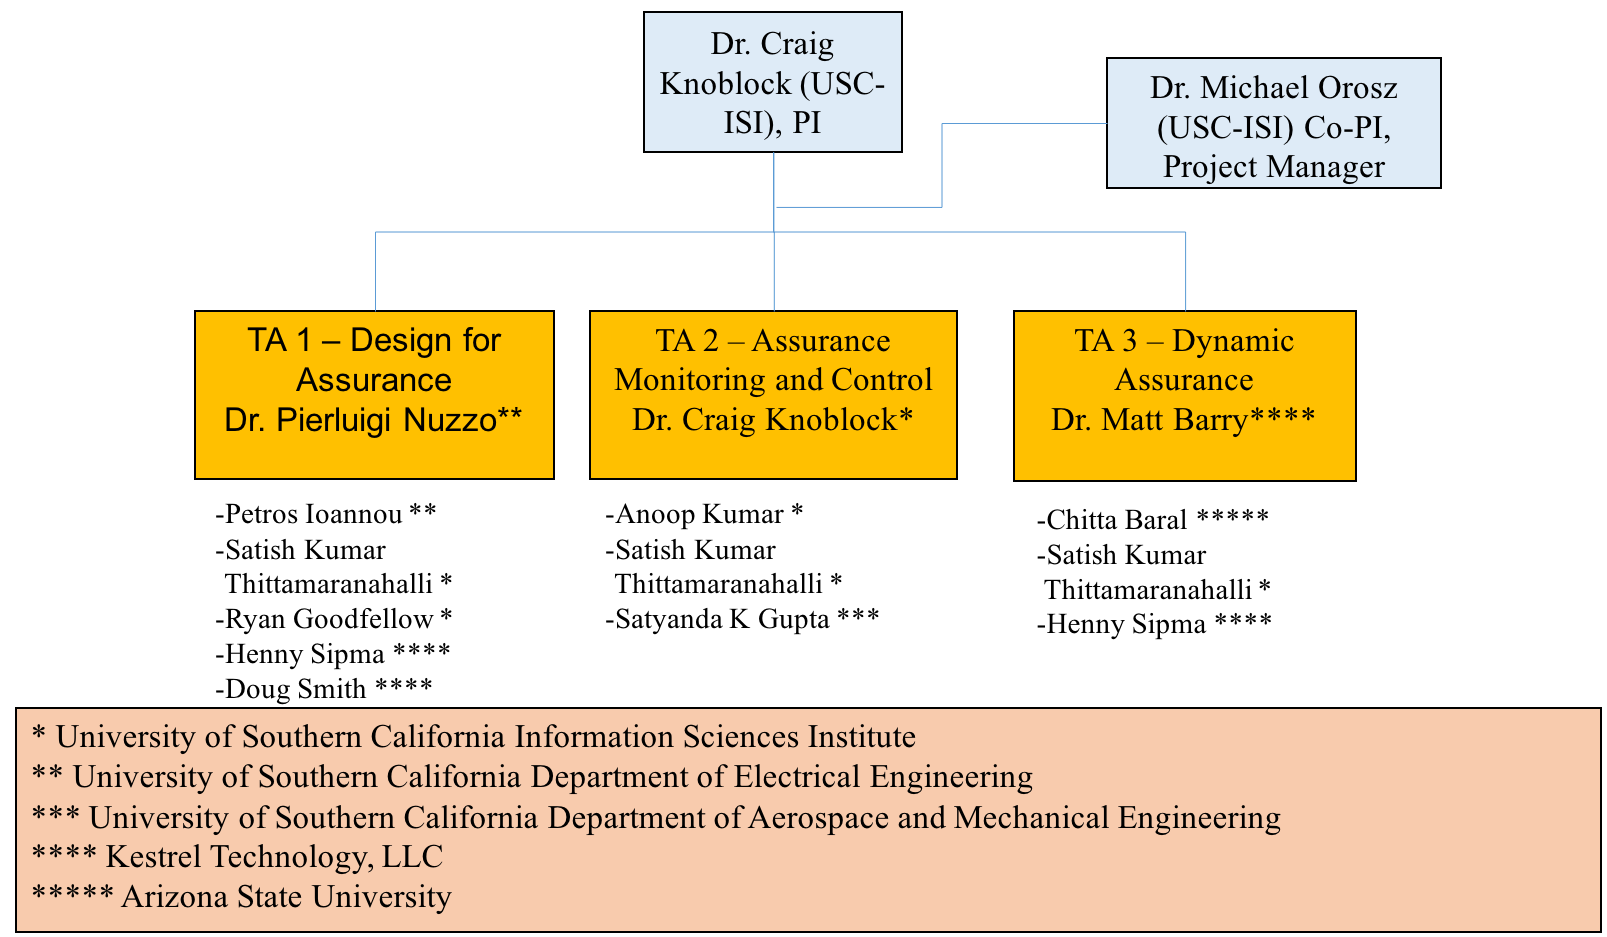
\includegraphics[width=6.0in]{./org-chart2.png}
\caption{\small Organization Chart}
\label{fig:org_chart}
\end{figure}

Coordination: To maximize collaboration and reduce risk to project failure from lack of communication and technical exchange, we plan to employ a wide variety of working styles and communication/coordination so that all can contribute.  At the core of our project will be regularly scheduled meetings bridging the diversely distributed team (Table~\ref{fig:Collaboration_Table}).  These meetings will address project status, identify challenges, implement risk mitigation strategies and participate in technology exchanges and system integration efforts (when appropriate)

\begin{table}[ht]
\caption{\small Project Meetings and Events}
  \centering
  {\footnotesize
\begin{tabular}{|m{3.15in}|m{3in}|} 
\hline
\textbf{Meeting} & \textbf{Frequency} 
\\\hline
Conference calls among investigators (discuss project status, address concerns and project risks) & Weekly
\\
\hline
Technical exchange and coordination meetings using Bluejeans or another videoconference technology & At least twice a month and more frequently as needed
  \\ 
\hline
Face-to-Face meetings (prior to P/I and demonstration meetings) & Every 3 to 6 months and more frequently (especially at the beginning of the project) as needed
 \\\cline{1-2}

\hline
\end{tabular}
}
\label{fig:Collaboration_Table}
\end{table}

\begin{table}[tbhp]
\caption{\small Key Project Team Member Responsibilities}
  \centering
  {\footnotesize
\begin{tabular}{| m{.75in} | m{3.9in}| m{1.5in}|} 
\hline
\textbf{Key Member} & \textbf{Responsibilities} & \textbf{Tasks} 
\\\hline
Dr.\ Craig Knoblock  & Principal Investigator responsible for project, leads TA 2 – Assurance Monitoring and Control.  Will lead the overall project and lead the TA2 team.  Served as the PI on many DARPA projects and has sucessfully led many large teams.    Effort on project:  25\% &
1.1.6, 1.2.2 1.2.3, 1.2.4, 1.3.4, 1.4.1, 
2.1.6, 2.2.2 2.2.3, 2.2.4, 2.3.4, 2.4.1, 
3.1.6, 3.2.2, 3.2.3, 3.2.4, 3.3.4, 3.4.1
\\
\hline
Dr.\ Michael Orosz & Co-Principal Investigator responsible managing the day-to-day operations of the project, assist technical teams as needed, coordinate with TA4 teams.    Has led many large complex multi-disciplined/multi-organizational projects in academic and industry environments.  Effort on project: 50\%
& 1.1.6, 2.1.6, 3.1.6, 1.4.1, 2.4.1, 3.4.1
  \\ 
\hline
Dr.\ Pierluigi Nuzzo 
& 
Co-Principal Investigator.  Leads the TA 1 - Design for Assurance team and conducts research on the formal methods for the design of the TA1 system.  Research experience on methodologies and tools for the design of cyber-physical systems; contracts, interfaces, and compositional methods for embedded system design; the application of automated formal methods and optimization theory to problems in embedded and cyber-physical systems.  Effort on project: 2 months/year (16.6\%)
& 
1.1.1, 2.1.1, 3.1.1 \\
\hline
Dr.\ Matthew Barry
& 
Key personnel.  Leads the TA 3 – Dynamic Assurance.   He will conduct the research on the dynamic assurance case language editors and parsers, the run-time system, and system integrations. Effort on project:  66\%
& 
1.3.2, 2.3.2, 3.3.2\\
\hline
Dr.\ Chitta Baral
& 
Key personnel responsible for learning assurance rules, supporting assurance rules with uncertainty and improving solver speed.  Expertise on ASP solvers, which will be used to reason about the assurance cases. Effort on project: 20\%
& 
1.3.1, 2.3.1, 3.3.1 \\
\hline
Dr.\ Doug Smith 
& 
Key personnel will support formal methods aspects of TA1, and lead the effort on abstract refinement. Expertise in field of automated correct-by-construction program generation.    Effort on project: 40\%
& 
1.1.5, 2.1.5, 3.1.5 \\
\hline
Dr.\ Henny Sipma
& 
Key personnel who will support the program verification tasks under TA1.  Will lead the effort on program verification.   Effort on project:  45\%
& 
1.1.5, 2.1.5, 3.1.5, 1.3.2, 2.3.2, 3.3.2 \\
\hline
Dr.\ Petros Ioannou
& 
Key personnel responsible providing and extending the assurance test bed, which will be available at the start of the project for autonomous vehicles.   Effort on project: 1 month/year (8.3\%)
& 
1.1.2, 2.1.2 (optional), 3.1.2 (optional)
\\
\hline
Dr.\ Satyandra Kumar Gupta
& 
Key Personnel providing autonomous command and control expertise to the TA-2 team.   Will lead the research on safety aware learning on TA2.   Past research on physics-aware decision making to facilitate automation.  Effort on project: 1 month/year (8.3\%)
& 
1.2.1, 2.2.1, 3.2.1 \\
\hline
Dr.\ Anoop Kumar 
& 
Key personnel providing support to the TA 2 project team.  Will lead the research on monitoring \& control and detecting distribution shifts.  Effort on project: 50\%
& 
1.2.1, 1.2.2, 1.2.3, 1.2.4, 2.2.1, 2.2.2, 2.2.3, 2.2.4, 3.2.1, 3.2.2, 3.2.3, 3.2.4\\
\hline
Dr.\ Satish Thittamaranahalli
& 
Key personnel developing scalable algorithms for TA1, TA2, and TA3 project teams.  Has extensive experience on scalable algorithm design, machine learning, and constraint reasoning.  Effort on project: 50\%
& 
1.2.1, 1.2.2, 1.2.3, 1.2.4, 2.2.1, 2.2.2, 2.2.3, 2.2.4, 3.2.1, 3.2.2, 3.2.3, 3.2.4, 1.1.4, 2.1.4, 3.1.4 \\
\hline
Dr.\ Ryan Goodfellow
& 
Key personnel providing support to the TA-1 project. Will lead the research on simulation-based testing.  Has extensive experience on simulation-based testing.  Effort on project:  30\%
& 
1.1.3, 2.1.3, 3.1.3 \\

\cline{1-2}

\hline
\end{tabular}
}
\label{fig:Table_Mgmt}
\end{table}



\newpage
\section{Personnel, Qualifications and Commitment}

{\bf Dr.\ Craig Knoblock}, the PI on this effort, is a Research Professor of both Computer Science and Spatial Sciences at the University of Southern California (USC) and Director of the Intelligent Systems Division at the USC Information Sciences Institute.   He received his Ph.D. from Carnegie Mellon University in computer science. 
%His research focuses on techniques for describing, acquiring, and exploiting the semantics of data.  
In previous projects he has worked on developing  scalable approaches to execution monitoring, accurate detection of sensor failures, and   automatic modeling and reconstruction of sensors.  He has published more than 300 journal articles, book chapters, and conference papers on these topics.  Dr. Knoblock is a Fellow of the Association for the Advancement of Artificial Intelligence (AAAI), a Distinguished Scientist of the Association of Computing Machinery (ACM), a Senior Member of IEEE, past President and Trustee of the International Joint Conference on Artificial Intelligence.
%and winner of the 2014 Robert S. Engelmore Award.  

{\bf Dr.\ Michael Orosz}, a Co-PI on this effort, is a Research Associate Professor of Civil and Environmental Engineering at the University of Southern California (USC) and Research Director of the Decision Systems Group at the USC Information Sciences Institute.  Dr. Orosz has over 30 years’ experience in commercial and government software development, basic and applied research, project management, academic research and has developed and deployed several commercially successful products.  His research interests are in machine learning and decision analytics as applied to intelligence analysis and autonomous command and control such as smart building controls.    Dr. Orosz has extensive experience in managing large complex multi-disciplined/multi-teamed research projects. %funded by DARPA, DHS, DoD, DoE, Industry, NASA, NRO, NSA and ONR.   
He received his Ph.D. in computer science from the University of California, Los Angeles.

{\bf Dr.\ Pierluigi Nuzzo}, a Co-PI on this project, is an Assistant Professor in the Department of Electrical Engineering at the University of Southern California. He received the Ph.D. in Electrical Engineering and Computer Sciences from the University of California at Berkeley. 
%in 2015, and the Laurea degree (MS) in electrical engineering (summa cum laude) from the University of Pisa, Italy, and the Sant'Anna School of Advanced Studies, Pisa, Italy.
%
%He has four years of research experience in analog and mixed signal circuit design as a researcher at IMEC, Leuven, Belgium, and over 10 years experience in design methodologies and tools for mixed-signal integrated circuits and cyber-physical systems, as a researcher at the University of Pisa, IMEC, UC Berkeley, and USC. 
His research interests
include: methodologies and tools for cyber-physical system and mixed-signal
system design; contracts, interfaces and compositional methods for embedded
system design; the application of formal methods and optimization theory to problems in embedded and cyber-physical systems and electronic design automation. 
%
Prof. Nuzzo received %First Place in the operational category and Best Overall
%Submission in the 2006 DAC/ISSCC Design Competition, 
a Marie Curie Fellowship
from the European Union in 2006, 
the University of California at Berkeley EECS
departmental fellowship in 2008, 
%the University of California at Berkeley Outstanding Graduate Student Instructor Award in 2013, 
the IBM Ph.D.
Fellowship in 2012 and 2014, 
%the Best Paper Award from the International Conference on Cyber-Physical Systems (ICCPS) in 2016, 
and the David J.~Sakrison Memorial Prize in 2016 for his doctoral research. 
%He is an author of 1 patent and over 60 publications.

{\bf Dr.\ Satyandra K. Gupta} is Smith International Professor in the Department of Aerospace and Mechanical Engineering at the University of Southern California. %Prior to joining the University of Southern California, he was a Professor in the Department of Mechanical Engineering and the Institute for Systems Research at the University of Maryland. He was the founding director of the Maryland Robotics Center and the Advanced Manufacturing Laboratory at the University of Maryland. 
He served as a program director for the National Robotics Initiative at the National Science Foundation from September 2012 to September 2014.  Dr. Gupta's interest is in the area of physics-aware decision making to facilitate automation. He has published more than 300 technical articles. He is a fellow of the American Society of Mechanical Engineers (ASME) and editor of ASME Journal of Computing and Information Science in Engineering. Dr. Gupta has received the Young Investigator Award from the Office of Naval Research in 2000, CAREER Award from the National Science Foundation in 2001, Presidential Early Career Award for Scientists and Engineers (PECASE) in 2001, Invention of the Year Award at the University of Maryland in 2007, Kos Ishii-Toshiba Award from ASME in 2011, and Excellence in Research Award from ASME in 2013.%, and Distinguished Alumnus Award from Indian Institute of Technology, Roorkee in 2014. %He has also received seven best paper awards at conferences.

{\bf Ryan Goodfellow} is a computer scientist at ISI working in combined cyber physical simulation and emulation platform development. His formal background is in simulation algorithms and modeling techniques using differential-algebraic equations (DAE). He has applied this knowledge in the CPS space by integrating DAE modeling languages and simulation engines with network testbeds to create comprehensive scientific experimentation platforms for cyber-physical systems. These experimentation platforms have been used in the power grid research space. %Ryan is a lead developer on the Deter network testbed, with a strong background in networked and distributed systems engineering. %He is also a combat veteran, serving as a non-commissioned officer and SIGINT team lead for a multi-functional intelligence team in Afghanistan.

{\bf Dr.\ Petros Ioannou} is a Professor in the Department of Electrical Engineering, Director of the Center for Advanced Transportation Technologies and Associate Director for Research for the DOT supported University Transportation Center at USC. He received his MS and PhD from the University of Illinois at Urbana Champaign in Mechanical and Electrical Engineering, respectively. His research interests are in robust adaptive control, vehicle dynamics and control, human factors and safety, automated vehicles, nonlinear systems and Intelligent transportation Systems.  He received the 2016 IEEE Transportation Technologies field award and the 2016 IEEE Control system society Transition to Practice Award. He is a Fellow of IEEE, IFAC and IET and author/coauthor of 8 books and over 400 papers.

{\bf Dr.\ Matthew Barry} will serve as lead for the TA3 tasks. %He will implement the dynamic assurance case language editors and parsers, the run-time system, and system integrations.  He will implement the assurance case arguments and the API for updating argument structure and content.  
Dr. Barry currently is CEO at Kestrel Technology LLC, and previously spent 20 years in NASA space mission operations at the Jet Propulsion Lab and Johnson Space Center.  At NASA Headquarters he led the introduction of dependability case requirements and plans for flight computing systems in upcoming manned space exploration missions, as well as the development of Agency-level software-related safety-critical control system requirements.  He recently served as a Principal Investigator on DHS/Cyber S\&T STAMP (Static Tool Analysis Modernization Program), DARPA CSFV (Crowd Sourced Formal Verification), three NASA Aeronautics R\&D projects, and the AFRL-sponsored Static Analysis of Numerical Algorithms project.  Dr. Barry earned BSME, MS, and PhD degrees in mechanical engineering, and an MBA degree, from Rice University.  

{\bf Dr.\ Henny Sipma} will support the program verification tasks under TA1.  %She is the key person behind the company's {\em KT Advance\/} and {\em KT Transferal\/} static analysis products, and the designer and programmer of the company's core {\em CodeHawk\/} abstract interpretation engine. 
Dr. Sipma currently is the CTO at Kestrel Technology LLC.  She has spent the past 10 years with Kestrel Technology as a static analysis expert; previously developed and taught static analysis techniques as senior research associate at Stanford University for eight years; and developed industrial process controls as an senior systems analyst at Shell.  She has been Principal Investigator or company lead on several recent R\&D projects for Federal agencies, including two projects under the IARPA STONESOUP (Securely Taking On New Executable Software of Uncertain Provenance) program; the DHS Cyber S\&T Gold Standard project; and the DARPA-sponsored STAC (Space-Time Analysis for Cybersecurity) and MUSE (Mining and Understanding Software Enclaves) programs.  Dr. Sipma earned 
%a BS degree in chemistry and an MS degree in chemical engineering at the University of Groningen in The Netherlands, and 
MS and PhD degrees in computer science from Stanford University.  

{\bf Dr.\ Douglas R.\ Smith} will support formal methods aspects of TA1, including the enforcement of safety properties and the generation of monitors.  He is President of Kestrel Technology LLC and Principal Scientist at Kestrel Institute.  He is a Fellow of the American Association of Artificial Intelligence (AAAI) and an ASE Fellow (Automated Software Engineering).  From 1986 to 2000, he taught an advanced graduate course on correct-by-construction software development at Stanford.  
%Dr. Smith has led the development of a series of software synthesis systems, including KIDS (Kestrel Interactive Development System), Specware, Designware, and Planware. 
%Applications domains have included a variety of complex high-performance planners and schedulers for the US Air Force.  He leads current projects on the generation of air mission plans and cyberoperations.  
Other recent projects focused on automated policy enforcement \cite{SmithD0703,SmithD08}, synthesis of secure network protocol codes, and the synthesis of high-performance constraint-solvers\cite{SmithD08c,SmithD13}.  Dr. Smith has over 30 years experience in the field of automated correct-by-construction program generation and has published over 100 papers. He has one patent.  He received the Ph.D. in Computer Science from Duke University% in 1979.  

{\bf Dr. Chitta Baral} is a Professor in the Department of Computer Science and Engineering at Arizona State University. He will support the TA3 efforts on Learning assurance rules, supporting assurance rules with uncertainty and improving solver speed. Dr. Baral has expertise in various aspects of autonomy and Artificial Intelligence. 
He wrote the first book on answer set programming (published by Cambridge University Press) the formal language behind our assurance rules. Some of his other works relevant to this proposal are: goal specification for autonomous systems, automatic construction of control rules for autonomous systems that satisfy given goals, combining machine learning with reasoning in various contexts, including image understanding. %He is the President of KR Inc. He is an associate editor of AIJ and has been an associate editor of JAIR.

{\bf Dr.\ Satish Kumar Thittamaranahalli (T. K. Satish Kumar)} leads the Collaboratory for Algorithmic Techniques and Artificial Intelligence (CATAI) at USC's Information Sciences Institute. He has published over 60 papers on numerous topics in Artificial Intelligence spanning such diverse areas as Constraint Reasoning, Planning and Scheduling, Probabilistic Reasoning, Robotics, Combinatorial Optimization, Approximation and Randomization, Heuristic Search, Model-Based Reasoning, Knowledge Representation and Spatio-Temporal Reasoning. %He %has served on the Program Committees of many international conferences in Artificial Intelligence
He and is a winner of the 2016 Best Robotics Paper Award and the 2005 Best Student Paper Award from the International Conference on Automated Planning and Scheduling. 
Dr. Kumar received his PhD in Computer Science from Stanford University. %In the past, he has also been a Visiting Student at the NASA Ames Research Center, a Postdoctoral Research Scholar at the University of California, Berkeley, a Research Scientist at the Institute for Human and Machine Cognition, a Visiting Assistant Professor at the University of West Florida, and a Senior Research and Development Scientist at Mission Critical Technologies.

\textbf{Dr.\ Anoop Kumar} is a senior computer scientist at USC ISI and has broad expertise in machine learning, statistical modeling, and software engineering.  Dr.\ Kumar is the technical lead on the DARPA RSPACE program and has played a vital role in developing a system that fuses air operations data from multiple sources, maintains world state, and issues warnings. Previously, he led the research and development of the BBN’s election forecasting system for the IARPA OSI program. %Dr.\ Kumar played a significant role in the DARPA DEFT program by developing a model to support integration of output from multiple NLP algorithms. He has contributed at the development to management levels on government research contracts and commercial projects. 
Dr.\ Kumar helped design and develop BBN's commercially available, hosted speech and medical transcription services offering. 

\begin{table}[!tbh]
\begin{footnotesize}
\vspace{-0.1in}

\begin{tabular}{lll}
\begin{tabular}[t]{|l|@{}c@{}|@{}c@{}|@{}c@{}|@{}c@{}|} \hline
Project & Status & \multicolumn{3}{ c| }{Hours} \\ \cline{3-5}
& & P1 & P2 & P3 \\ \hline



\multicolumn{5}{ |c| }{ \textbf{Craig Knoblock} } \\ \cline{1-5}
Safeguard & Pro & 770 & 641 & 641 \\ \cline{1-5}
ELICIT & Cur & 308 & 256 & 120 \\ \cline{1-5}
WTNIC & Cur & 11 & 0 & 0 \\ \cline{1-5}
EFFECT & Cur & 641 & 107 & 0 \\ \cline{1-5}
LinkedMaps & Cur & 203 & 25 & 0 \\ \cline{1-5}
PRINCESS & Cur & 608 & 96 & 0 \\ \cline{1-5}
SCHARP & Cur & 481 & 54 & 0 \\ \cline{1-5}
MINT & Pen & 650 & 534 & 285 \\ \cline{1-5}

\multicolumn{5}{ |c| }{ \textbf{Michael Orosz} } \\ \cline{1-5}
Safeguard & Pro & 1560 & 1300 & 1300  \\ \cline{1-5}
SMC/SY & Cur & 1803 & 0 & 0  \\ \cline{1-5}

\multicolumn{5}{ |c| }{ \textbf{Matthew Barry} } \\ \cline{1-5}
Safeguard & Pro & 2078 & 1690 & 1554 \\ \cline{1-5}
Starlite & Cur & 1840 & 1692 & 0 \\ \cline{1-5}



\multicolumn{5}{ |c| }{ \textbf{Anoop Kumar} } \\ \cline{1-5}
Safeguard & Pro & 1560 & 1300 & 1300 \\ \cline{1-5}

\end{tabular}
&
\begin{tabular}[t]{|l|@{}c@{}|@{}c@{}|@{}c@{}|@{}c@{}|} \hline
Project & Status & \multicolumn{3}{ c| }{Hours} \\ \cline{3-5}
& & P1 & P2 & P3 \\ \hline

\multicolumn{5}{ |c| }{ \textbf{Pierluigi Nuzzo} } \\ \cline{1-5}
Safeguard & Pro & 520 & 433 & 433  \\ \cline{1-5}
Mirage & Cur & 433 & 0 & 0  \\ \cline{1-5}

\multicolumn{5}{ |c| }{ \textbf{Satyandra Gupta} } \\ \cline{1-5}
Safeguard & Pro & 260 & 217 & 217 \\ \cline{1-5}
Human   & Cur & 22 & 0 & 0 \\ \cline{1-5}
Vehicles & Cur & 36 & 0 & 0 \\ \cline{1-5}
Robot & Cur & 116 & 0 & 0 \\ \cline{1-5}
Assembly & Cur & 33 & 0 & 0 \\ \cline{1-5}
Solar & Cur & 4 & 0 & 0 \\ \cline{1-5}

\multicolumn{5}{ |c| }{ \textbf{Petros Ioannou} } \\ \cline{1-5}
Safeguard & Pro & 260 & 217 & 217 \\ \cline{1-5}
CPS & Cur & 130 & 0 & 0 \\ \cline{1-5}

\multicolumn{5}{ |c| }{ \textbf{Ryan Goodfellow} } \\ \cline{1-5}
Safeguard & Pro & 936 & 780 & 780 \\ \cline{1-5}
STEAM & Cur & 416 & 0 & 0 \\ \cline{1-5}


\end{tabular}
&
\begin{tabular}[t]{|l|@{}c@{}|@{}c@{}|@{}c@{}|@{}c@{}|} \hline
Project & Status & \multicolumn{3}{ c| }{Hours} \\ \cline{3-5}
& & P1 & P2 & P3 \\ \hline

\multicolumn{5}{ |c| }{ \textbf{Chitta Baral} } \\ \cline{1-5}
Safeguard & Pro & 659 & 485 & 485 \\ \cline{1-5}
PostdocBP & Cur & 176 & 0 & 0 \\ \cline{1-5}
Languages & Pen & 528 & 264 & 264 \\ \cline{1-5}
CAREER & Pen & 88 & 44 & 44 \\ \cline{1-5}
CHS & Pen & 510 & 255 & 0 \\ \cline{1-5}

\multicolumn{5}{ |c| }{ \textbf{Doug Smith} } \\ \cline{1-5}
Safeguard & Pro & 1222 & 984 & 840 \\ \cline{1-5}
RSPACE & Cur & 342 & 0 & 0 \\ 
\cline{1-5}
PLANX & Cur & 154 & 0 & 0 \\ 
\cline{1-5}
HACCS & Pen & 923 & 769 & 769 \\ 
\cline{1-5}

\multicolumn{5}{ |c| }{ \textbf{Henny Sipma} } \\ \cline{1-5}
Safeguard & Pro & 1372 & 962 & 840 \\ \cline{1-5}
STAC & Cur & 797 & 0 & 0 \\ \cline{1-5}

\multicolumn{5}{ |c| }{ \textbf{Satish Thittamaranahalli} } \\ \cline{1-5}
Safeguard & Pro & 1560 & 1300 & 1300 \\ \cline{1-5}
MapF & Cur & 103 & 103 & 0 \\ \cline{1-5}

\end{tabular}
\end{tabular}

\end{footnotesize}
\caption{Individual commitments of key personnel}
\label{tab:Commitments}
\vspace{-0.2in}
\end{table}

\clearpage
\newpage
\section{Capabilities}


%\subsection{University of Southern California}
USC has strengths in number of areas that are closely related to the proposed work:
\begin{itemize}[itemsep=0pt,leftmargin=*]
\item Dr.\ Nuzzo 
%has over 10-year research experience in embedded system design, from mixed-signal chip design (analog-to-digital converters, frequency synthesizers, software-defined radio), to methodologies and tools for mixed-signal integrated circuits and Cyber-Physical Systems (CPSs), and the application of formal methods and optimization theory to problems in embedded and cyber-physical systems and electronic design automation.  
%His doctoral work 
has done extensive research on contracts and compositional methods for heterogeneous system design and design space exploration, with application to aircraft electric power systems and environmental control systems. His work has helped transition rigorous system design foundations, innovative design methodologies, and new systems engineering paradigms to industry (IBM, United Technologies). 
\item Dr.\ Satyandra K. Gupta has worked on autonomous surface vehicles, autonomous ground vehicles for operation on rugged terrains, and autonomous flapping wing aerial vehicles.   His group has developed a hierarchal decision making approach for realizing autonomous systems. 
%This approach combines task planning and assignment, deliberative trajectory planning, reactive collision avoidance behaviors, and trajectory tracking control layers. 
His group has also developed new methods for learning reactive behaviors in adversarial environments and COLREGS compliant trajectory planning. \item Dr.\ Knoblock has developed methods that learn the relationships between sensors to both identify failures and changes in sensor and reconstruct those sensors, providing estimates of the accuracy of the reconstructed sensors.  
\item Ryan Goodfellow has extensive experience in simulation based testing through high-fidelity CPS testbed environment development and operation, using the Deter network testbed as the core which has supported several large scale government projects from a variety of agencies and thousands of users. %we have developed sophisticated CPS experiments under programs such as NFS RIPS, NIST SmartCities and the DHS Cybersecurity showcase.
\item Dr.\ Ioannou %helped  design and implement adaptive cruise control systems in collaboration with Ford Motor Company, which was commercialized four years before any other company. He 
worked on several DOT funded projects on automated vehicles and intelligent highway systems where he demonstrated his vehicle control designs for safety and performance on actual automated vehicles in test trucks and I-15 highway.
\item Drs.\ Knoblock, Kumar, and Thittamaranahalli have developed highly scalable approaches for monitoring message traffic to identify potential problems and issue warnings and alerts. 
\item Dr. Thittamaranahalli has developed state-of-the-art methods for efficiently solving large-scale search and optimization problems. %These techniques will be applicable in TA2 for safety-aware learning and planning, in TA2 for assurance monitoring and control, and in TA3 for dynamic assessment of assurance cases.

\end{itemize}
%\subsection{Kestrel Technology LLC}

Kestrel Technology's strength is in program analysis, specifically static analysis of both source and binary targets.  The company performs applied R\&D and product development for a variety of static analysis applications  pivoting primarily on the abstract interpretation technique.  The company recently initiated development of program analysis applications using logical equivalence techniques. As a provider of verification evidence in the form of mathematical proofs, the company also has expertise in the design and development of assurance case arguments for high-integrity systems using such evidence. %The company is engaged in a partnership with Wind River Systems to develop program analysis tools for its embedded system developers.  Many of Wind River's customers must develop their products under safety and certification standards, including those using safety cases.  

   

%\subsection{Arizona State University}
Chitta Baral at Arizona State University has developed various software to learn assurance rules and various ASP solvers, which he has made available as open-source.

Most of the software carried forward for implementation or derivation is open source.  The single exception is Kestrel Technology's {\it KT Advance\/} static analysis tool (TA1), in particular the abstract interpretation engine therein, which is company proprietary and is US EAR export-controlled.   
%Owing to mixed funding for the development of that technology 
We will continue to provide the Federal government a restricted use license for that particular item.

There are no specialized facilities, data, or GFE required for this effort. 

\include{sow}
\include{milestones}

% \section{Level of Effort by Task \textcolor{red}{[Mike/Lisa - 1 pages]}}

% \textcolor{blue}{
% \begin{itemize}
% \item Will be a separate spreadsheet
% \item
% \end{itemize}
% }

\include{appendix_a}

%\section{Appendix B \textcolor{red}{[No Page Count]}}

\section{References}
\bibliographystyle{acm} 
\bibliography{TA3/ta3,TA2/ta2,TA1/ta1}
\end{document}
%%\documentclass[a4paper]{article}
%\documentclass[12pt]{article}
\documentclass[12pt]{dod-blank}

%% Language and font encodings
\usepackage[english]{babel}
\usepackage[utf8x]{inputenc}
\usepackage[T1]{fontenc}

%% Sets page size and margins
%%\usepackage[a4paper,top=3cm,bottom=2cm,left=3cm,right=3cm,marginparwidth=1.75cm]{geometry}
%\usepackage[top=1in, bottom=1in, left=1in, right=1in]{geometry}



%% Useful packages
\usepackage{amsmath}
\usepackage{graphicx}
  \graphicspath{{.}{./image/}}
  \DeclareGraphicsExtensions{.png,.jpg} 
\usepackage[colorinlistoftodos]{todonotes}
\usepackage[colorlinks=true, allcolors=blue]{hyperref}
\usepackage{tabularx}
\usepackage{multirow}
\usepackage{tabulary}
\usepackage{float}
\usepackage{wrapfig}
\usepackage[export]{adjustbox}
\usepackage{comment}
\usepackage{tabularx}
\usepackage{multirow}
\usepackage{tabulary}
\usepackage{enumitem}

\usepackage{listings}
\usepackage{color}
\usepackage{array}
\usepackage{subcaption}
\usepackage{xcolor}




\renewcommand{\textfraction}{0}
\renewcommand{\topfraction}{1.0}
\renewcommand{\bottomfraction}{1.0}

\usepackage{longtable}
%% macros
\newif\iffinal
\finaltrue
\iffinal
  
    \newcommand\baareq[1]{}
    \newcommand\baades[1]{}
 
 
\else
    \definecolor{darkgreen}{rgb}{0,0.4,0}
    \definecolor{darkcyan}{rgb}{0,0.4,0.4}
    \definecolor{darkblue}{rgb}{0,0,0.5}
    
    \newcommand\baareq[1]{{\color{darkcyan}[\textbf{Requirement:} #1]}}
    \newcommand\baades[1]{{\color{darkcyan}[\textbf{Description:} #1]}}
 
\fi




\def\naive{na\"{\i}ve}



\lstset{ 
  backgroundcolor=\color{white},   % choose the background color; you must add \usepackage{color} or \usepackage{xcolor}
  basicstyle=\footnotesize\ttfamily,            % the size of the fonts that are used for the code
  breakatwhitespace=false,         % sets if automatic breaks should only happen at whitespace
  breaklines=true,                 % sets automatic line breaking
  captionpos=b,                    % sets the caption-position to bottom
  commentstyle=\color{mygreen},    % comment style
  % deletekeywords={...},            % if you want to delete keywords from the given language
  escapeinside={\%*}{*)},          % if you want to add LaTeX within your code
  extendedchars=true,              % lets you use non-ASCII characters; for 8-bits encodings only, does not work with UTF-8
  frame=single,	                   % adds a frame around the code
  keepspaces=false,                 % keeps spaces in text, useful for keeping indentation of code (possibly needs columns=flexible)
  keywordstyle=\color{blue}\bfseries\underbar,       % keyword style
  language=Prolog,                 % the language of the code
  % morekeywords={if,and},        % if you want to add more keywords to the set
  numbers=none,                    % where to put the line-numbers; possible values are (none, left, right)
  numbersep=5pt,                   % how far the line-numbers are from the code
  numberstyle=\tiny\color{mygray}, % the style that is used for the line-numbers
  rulecolor=\color{black},         % if not set, the frame-color may be changed on line-breaks within not-black text
  showspaces=false,                % show spaces everywhere adding particular underscores; it overrides 'showstringspaces'
  showstringspaces=false,          % underline spaces within strings only
  showtabs=false,                  % show tabs within strings adding particular underscores
  stepnumber=2,                    % the step between two line-numbers. If it's 1, each line will be numbered
  stringstyle=\color{mymauve},     % string literal style
  tabsize=2,	                   % sets default tabsize to 2 spaces
  title=\lstname                   % show the filename of files included with \lstinputlisting; also try caption instead of title
}

% apply trick for additional keywords for our AC DSL
\lstset{
	emph={for, if, and, or},
    emphstyle={\color{blue}\bfseries\underbar}
}




\title{DARPA Assured Autonomy}
\author{Technical Volume- \textcolor{red}{Thirty-Eight (38) pages max}}

\begin{document}
\pagenumbering{roman}
\include{cover}

\newpage
\section{Table of Contents}
\tableofcontents

\newpage
\pagenumbering{arabic}
\section{Executive Summary}
As we rapidly move into a world where machine learning plays a central role in realizing autonomous systems, it is becoming increasingly important to develop techniques that assure that these systems will operate safely and perform as expected. Current approaches are limited to providing assurance for systems with limited or no  learning capabilities. In this context, DARPA's Assured Autonomy BAA seeks to \emph{develop rigorous design and analysis technologies for continual assurance of learning-enabled autonomous systems}. USC in collaboration with Kestrel Technology and ASU is pleased to submit a comprehensive TA1, TA2, and TA3 proposal entitled \emph{``Assured Autonomy for Learning Enabled Vehicles (Safeguard).''} We plan to provide an end-to-end solution to support autonomous systems with learning-enabled components, ranging from design technologies for assurance, to assurance monitoring and control techniques, to representation and online evaluation of assurance cases. We have assembled a strong team of experts that cover the range of technologies that are required to create such an end-to-end system. If successful, the project will provide the technologies for building the next-generation of learning-enabled autonomous systems.  The entire project will take four years and cost \textcolor{red}{\$??}, with an initial version completed at the end of Phase I and successive versions with additional capabilities and improved scalability at the end of Phase II and Phase III.  

In the remainder of this section, we first introduce an  unmanned surface vehicle scenario that will be used throughout the proposal to describe the approach.  Next, we describe our approach to design, monitoring, and dynamic assurance. Finally, we introduce the team involved in the project. 

\textbf{Motivating Scenario.} Consider an autonomous unmanned surface vehicle (USV) guarding a valuable asset in the ocean when an unknown vehicle  approaches the security perimeter, under challenging weather conditions. In this scenario, the USV is required to approach the intruding vehicle, issue a warning signal, and escort it to a safe distance from the controlled area. However, as the USV has no a priori knowledge of its external environment behaviors (e.g., water depth, waves, wind, current, visibility), pre-computing a feasible trajectory, let alone optimal, becomes a non-trivial problem. For trajectory planning, the USV must continuously perform the following tasks:
\begin{itemize}[itemsep=0pt,leftmargin=*]
 \item Sense the current state of the surrounding environment (e.g., water depth, waves, wind, current, visibility) and estimate its own maneuverability constraints (e.g., braking distance, available acceleration, maximum velocity, turning radius, turning rate, safety distance) based on the state of the environment;      
\item Sense the static obstacles in the sensor range and generate a traversability map;
\item Sense the moving obstacles and classify them;   
\item Predict future trajectories of moving obstacles; 
\item Determine if any of the COLREGS \cite{commandant1999international} rules will be in effect with respect to one or more of the nearby vessels and identify the vessels with the right of way.    
\end{itemize}
The above information will be used by the trajectory planner to compute an initial trajectory, which will be continuously refined as the USV gathers additional information.
% It is not possible for the USV to be tested in every possible environment. 
The USV will use learning enabled components to take  decisions as it encounters new situations, such as  
\begin{itemize}[itemsep=0pt,leftmargin=*]
\item Classifiers to identify moving obstacles based on physical appearance and motion signatures,
\item Algorithms to estimate the sensor capabilities in adverse weather conditions,   
\item Algorithms to accurately estimate uncertainty in the environment, 
\item Classifiers to generate traversability maps,
\item Prediction of external vessel behaviors based on motion histories, 
\item Reinforcement learning  to ensure COLREGS compliance of maneuvers,  
\item Algorithms to learning pursuit behaviors.  
\end{itemize}
Learning enabled components will interact with each other in complex ways, where a misclassification error in one component may eventually compromise the entire mission.   
% We will need to make sure that each learning enabled components has a run-time monitor that will ensure that the assumptions made by the learning-enabled component remain valid and prevent erroneous learning. 
% For example, if the vehicle is exhibiting significant error in trajectory tracking, then simply downgrading the trajectory tracking error value may not be a good option.  The failure of prediction of trajectory tracking error might be due to the presence of a significant wake caused by a nearby vessel. The presence of the nearby vessel can be used to explain the degradation in trajectory tracking performance. As the vessel moves away, we can expect the trajectory tracking performance to return to the predicted level.  
While exhaustive validation of learning-enabled cyber-physical systems (LE-CPSs) is a prohibitive task~\cite{Kalra16},
their complexity, heterogeneity, and highly dynamic nature
make it challenging to even leverage existing model-based development techniques to effectively assess system correctness 
% dependability, 
at design time or enforce it at runtime.

\textbf{Design for Assurance.} Safeguard uses a platform-based design approach~\cite{Nuzzo15b} to organize the design process for a LE-CPS and to build assurance cases. Composite models are developed at several levels of abstraction,
from top-level system requirements and safety constraints down to the
implementation level.  Intermediate levels add detail to the levels
above.  The different levels are connected by refinement mappings that
allow properties established at one level to be preserved at the next
level (see Figures~\ref{fig:methodology} and~\ref{fig:assurance}).

Contracts are used to formally specify components and composite models
in terms of (1) Assumptions -- the assumed behaviors of the
environment and the behaviors of other components, and (2) Guarantees
-- the behavior properties that a model guarantees if it operates in a
context that satisfies its assumptions.  A calculus of contracts
allows horizontal composition of contracts to generate contracts for
composite models.  Vertical contracts are used to specify the mapping
or refinement relation between models at different levels of
abstraction.  The system design process starts with a high-level
contract that expresses overall system assumptions and requirements.
Subsequent levels express models with increasing detail until the
lowest level expresses the system in terms of hardware components and
their software controllers.

The assurance case for a CPS arises from the horizontal and vertical
structure of the design in several ways.  The components used within a
particular level are either (1) synthesized using
correct-by-construction design tools together with proofs, (2) derived
statically or dynamically using safety-aware machine-learning
techniques, (3) written manually and verified by analysis tools, or
(4) written manually and validated by extensive testing.  The
assurance case for the whole reflects its compositional structure.  We
anticipate that well-specified contracts together with the calculus of
contracts will eliminate well-known problems with unexpected emergent
behaviors in CPS systems.

The assurance case for the lowest-layer design arises from both the
intra-level assurance and from properties and their proofs that are
preserved under the refinement mapping from the top-level
requirements.  The refinement mappings between model layers will be
constructed using a variety of techniques.  A contract at an abstract
level can be mapped to a component or refined contract by (1)
retrieval of pre-verified components from a platform library, (2)
synthesis using correct-by-construction design and optimization tools,
or (3) manual coding to satisfy a contract.  The mapping of a
composite model will be composed from the mappings of its constituent
components or contracts.  When a composite model cannot be mapped
compositionally to the next level, it will be generated using
correct-by-construction design and optimization tools.

\textbf{Assurance Monitoring and Control.}
We provide an integrated framework for safety-aware learning, assurance monitoring and control, detecting distribution shifts. Three major components offer an efficient TA2 architecture as well as interfaces with TA1 and TA3, that is, (a) safety-aware learning and planning, (b) assurance monitors for guarding architectural and safety constraints; and (c) distribution shift detection.

We will develop a new learning-enabled online decision-making framework that allows opportunistically composing a sequence of actions (maneuvers) to reduce uncertainty in the system capability model without suspending the progress toward the mission goals or compromising safety. Each candidate action is evaluated based on three criteria: (1) the risk of violating a safety constraint using the current uncertainties in the parameter estimates; (2) its relevance to the mission goals; (3)  its expected information gain, i.e., reduction in uncertainty, with respect to the parameter estimates. These evaluations are combined to produce a cumulative mission utility value for each action that drives our learning-enabled decision-making framework. The problem of generating and evaluating sequences of actions can be posed in several way. For example, it can be solved using a branch-and-bound search method like Anytime A*, or formulated with the finite-horizon Markov Decision Process (MDP) framework. We will develop new scalable search strategies to solve this problem efficiently, by potentially evaluating a recent method developed at USC, called FastMap, that can significantly improve the execution time. 

We will develop monitors for architectural and safety constraints. 
% While these constraints can be checked over and over again as sensor information flow in, this naive strategy accounts for a lot of computational overhead. 
To achieve scalability and decrease the overhead, we propose the application of a technique that we currently use in DARPA's RSPACE program, which leverages a physical model of the vehicles dynamics and its interactions with the environment to efficiently determine the readout frequency. We propose two  extensions of this basic idea. First, we will use the theory of Variable Elimination to prioritize which variables to monitor, e.g., controllable, versus uncontrollable, adversarially controlled, or unobservable variables. Second, we invoke the dynamic assessment of assurance cases only when needed. This  decreases the number of times dynamic assessment of assurance cases is initiated as well as the communication bandwidth between the TA2 and TA3 components.

Finally, we will identify a distribution shift by combining statistical and machine learning techniques to differentiate between environmental and sensor changes. We will exploit a categorization of the shifts based on their cause and duration as well as extend our earlier work on detecting and mitigating sensor failures for all types of monitored variables.  

\textbf{Dynamic Assurance:} The Safeguard {\em design for assurance\/} activity takes a systems-theoretic stance toward safety.  Consequently, it presumes that safety is an emergent property of the system, and that hazards can present themselves through unintended interactions and performance violations in addition to causal events such as component failures.  Our design approach includes consideration of intent as well as hazard analysis and mitigation.  The artifacts from these activities populate contracts and assumptions for the dynamic assurance case.  
We thus build safety into the product by working at a systems-level viewpoint, using lexicon and design patterns familiar to both hardware and software engineers; safety is an emergent property of the system, not an afterthought.  
As system behavior evolves during runtime owing to learning, threats, degradation, or some other factor, the dynamic assurance case identifies whether the safety constraints continue to be satisfied.  If not, it provides notifications or issues recovery instructions directly from a lookup table.

Our implementation of the dynamic assurance case employs a declarative knowledge base inference engine and a domain-specific language tailored to our approach.  We have used them successfully for assurance case tool sets and arguments, and will extend them to reason about uncertainty and learning.  Our approach to achieve scalability is to specialize solvers toward modularity and to take advantage of domain knowledge.  Specifically, we will develop answer set programming techniques for context-dependent learning for reasoning about the learning-enabled components as well as learning assurance rules.  We will develop new formalisms for uncertainty to include causality, using weights for computing probabilities, and probabilistic non-monotonicity.  To achieve scaling objectives we will implement specializations using modularity, weighted CSPs, and message passing. 

% The system safety constraints revealed from that design become the key elements of our dynamic assurance case.  Our verification tools ensure the constraints are relevant, identifiable, and their implementation and effect observable.  

\textbf{Team.} We have assembled a team that is exceptionally well-qualified to build the proposed Safeguard system.  The team will be led by Dr.\ Craig Knoblock, the Principal Investigator for the effort, who currently leads the Intelligent Systems Division at the Information Sciences Institute.  He has led many large DARPA and IARPA projects over the years and has a strong track record in conducting leading edge research and then transitioning the technology to commercial use.  He will be supported by Dr.\ Michael Orosz as the Project Manager, who also has  experience in managing large research projects and on autonomous systems.  The TA1 team will be led by Dr.\ Pierluigi Nuzzo, who is an expert in embedded system design methodologies and the  application of formal methods to cyber-physical systems.  The TA1 team also includes Dr.\ Doug Smith, who has spent many years working on scalable correct-by-construction techniques and Dr.\ Henny Sipma, who has significant experience in applying program verification methods to real-world problems.  The TA1 team also includes Ryan Goodfellow, who has done a large amount of work on simulation-based testing.  The TA2 team will be led by Dr.\ Knoblock who has worked on topics related to both monitoring and detecting distribution changes.  He will be supported by Dr.\ Satyandra Gupta, who is an expert on autonomous surface vehicles as well as on safety-aware learning. He will also be supported by Drs.\ Anoop Kumar and Satish Thittamaranahalli, who have also previously worked on efficient methods for execution monitoring.  The TA3 team will be lead by Dr.\ Matthew Barry, who has experience in creating the technologies for assurance cases.  He will be supported by Dr.\ Chitta Baral, who is an expert on ASP solvers and by Dr.\ Thittamaranahalli who is an expert on SAT solvers, both of which will be applied to provide scalable assurance case reasoning.  Finally, Dr.\ Petros Ioannou, who is an expert on control systems for autonomous vehicles will provide an autonomous vehicle platform, which will form the focus of our work until the TA4 teams provide additional vehicle platforms for development.  

\newpage
\section{Innovative Claims and Deliverables}

In this project we will develop and build an end-to-end system for assured autonomy.  This section describes the key innovations by technical area and then the overall deliverables of the project.

\paragraph{Design for Assurance}

\begin{itemize}[itemsep=0pt,leftmargin=*]
\item We address the LE-CPS design challenges via a holistic approach that can contextually generate design artifacts and assurance cases. We develop a compositional, contract-based modeling framework, methods, and tools to support the design process from system-level requirement capture,  formalization, and analysis, to the generation, testing, and continual monitoring of software and hardware artifacts in feedback loop with a physical process.

\item We develop compositional abstractions and interfaces (vertical contracts) that can  bridge heterogeneous formalisms and heterogeneous decomposition architectures to make system analysis and synthesis tractable, consistently combine different verification and synthesis methods at design time, and provide seamless support for dynamic assurance at run time. %We aim to quantitatively capture the confidence in the satisfaction of requirements under uncertain or unknown conditions, and resilience properties of  systems at different abstraction levels, to enable trade-off evaluation between resilience, performance, and cost.

\item We develop a unifying framework and efficient algorithms to reason about the combination of discrete and continuous dynamics and constraints in the presence of uncertainties in LE-CPS using a satisfiability modulo convex approach~\cite{Shoukry2017} for contract-based system verification and scalable trajectory planning.  

\item We provide an environment for high-fidelity CPS testing, in which production-ready software, e.g.,  safety-critical learning and control, may be deployed and tested 
% by extending the Cypress testbed environment \cite{Goodfellow2015Cypress:Systems} 
with time dilation facilities, so that it synchronizes with a physical simulation that is not necessarily running in real time, while still having the perception of real time.

\item We 
% These facilities allow a cyber system to be  
propose an approach for unanticipated behavior space identification and test coverage maximization which leverages results from the theory of differential algebraic equation (DAE)~\cite{Berger2013ControllabilitySurvey,Ilchmann2005ATheory,BergerOnSystems,Lamour2013} 
to prune the behavior search space and identify smaller regions of interest for efficient simulation-based testing. 
% We then compute the intersection of these two behavior spaces and restrict our simulation based testing search space to this subspace.
\end{itemize}

\paragraph{Assurance Monitoring and Control}

\begin{itemize}[itemsep=0pt,leftmargin=*]
\item 
%We integrate safety-aware learning into the overall decision making problem. The goal is to maximize mission utility without violating the safety constraints. 
Our safety-aware learning framework enables the system to opportunistically select and execute actions to assist the learning-enabled component in reducing model uncertainty without compromising safety or deviating from the mission goals. The value of uncertainty reduction is explicitly incorporated in the optimization process for selecting the best action.  
\item For safety-aware learning, we propose the idea of preprocessing the search space of the problem domain before queries and observations come in. With such a linear-time preprocessing phase, the performance of search and optimization algorithms can be significantly boosted. For example, in regular A* search, the intensional or extensional search space can be preprocessed in near-linear time to yield an embedding of each state as a point in Euclidean space~\cite{cujakk}. Then, when the query comes in, A* search can make use of these Euclidean distances as heuristic distances between two states to yield order-of-magnitude speedups. 
%In Anytime A* for safety-aware learning and planning, this leads to a significantly better quality of actions chosen within a time limit, and in the MDP framework, the same ideas can be used to improve the convergence of Bellman updates for safety-aware Reinforcement Learning.
\item As massive amounts of sensor information flow in, it is imperative for us to efficiently process this information for monitoring architectural and safety constraints. Building on our past work on similar tasks, we propose novel technologies for efficiently monitoring constraints. These algorithms can yield an exponential reduction in the amount of sensor data that needs to be processed. Doing this also reduces the message complexities between the various modules. %We also propose to use the theory of Variable Elimination (VE) to monitor constraints with uncontrollable, adversarially controlled, and/or unobservable variables. VE yields a substrate constraint to monitor that characterizes a dominant strategy of the controllable variables over the uncontrollable, adversarially controlled, and/or unobservable variables.
\item We will develop techniques to identify  distributional shifts and determine the underlying cause (e.g., change in environment, sensor failure,   etc.), as well as strategies for handling the various distributional shifts.   Notably, we propose to build on our past work and use compact representations to exploit historical data to identify distributional shifts.
\end{itemize}

\paragraph{Dynamic Assurance}

\begin{itemize}[itemsep=0pt,leftmargin=*]

\item We demonstrate the integration of dynamic assurance for safety-critical learning-enabled dynamic systems in which evolutionary behaviors are expected and tolerated as a property of the functionality.   The impact will be consequential contributions safety-critical dynamic systems in which evolutionary behaviors are expected and tolerated as portion of the functionality.   
\item We implement dynamic assurance by combining features of system safety, formal methods, logic programming, uncertain reasoning, and domain-specific languages.  We populate assurance case arguments at several levels of modeling and implementation abstraction, using the analysis results to produce design-time evidence supporting assurance claims.  
%We provide automated reasoning about the assurance case itself to produce verification, consistency, and completeness results for the argument.  Dynamic assurance results then yield trusted explanations of whether safety constraints and assumptions and other contracts still hold during the collection of runtime evidence from monitors. 
\item We develop and demonstrate ASP formalisms crucial to applications in dynamic assurance. We demonstrate the suitability of the technology especially for assurance case arguments owing to the improved legibility, consistency and completeness checks, handling of uncertain and default reasoning, and scalability.  
%We will produce modularized solvers for enhanced performance based on recent algorithmic developments in exploiting structure, kernelization, and message passing. We provide a formalism to enable learning of assurance rules. 
We provide a novel approach to handling uncertainty that provides the ability to do causal and counter-factual reasoning as well as probabilistic non-monotonicity.  Overcoming limitations of traditional inductive logic techniques, we develop a novel iterative and incremental approach based on context dependent learning. 
\end{itemize}

\paragraph{Deliverables}
During the course of this project, we will build and deliver a fully-operational system that covers all three of the technical areas.  The detailed capabilities of this system are described in the individual technical sections.  The resulting system will be available as open source under a permissive license, which will allow other organizations to use the work, extend it in new directions, and even commercialize the software.  Kestrel Technology has significant experience in this space and has built and applied these types of technologies to a variety of real world tasks.  Kestrel is ideally suited to pursue commercial uses of this technology and the permissive license will facilitate exploring these opportunities since there will be no need to negotiate intellectual property rights.  

\newpage
\section{Technical Plan}
\input{./TA1/main}
\input{./TA2/main}
\input{./TA3/main}
\clearpage
\newpage


\section{Management Plan}


The Principal Investigator for this effort is Dr. Craig Knoblock who is responsible for all aspects of the effort, will coordinate the parallel team efforts, and will ensure high levels of performance from individual team members.  The Co-P/I, Dr. Michael Orosz, will provide project management and will assist all performers in the execution of the project.    The project team is divided into three working groups (Figure~\ref{fig:org_chart}) corresponding to Technical Areas 1-3, however, members of each team contribute across all project activities.   Table~\ref{fig:Table_Mgmt} defines the major contributions of each project team member to the project tasks.

\begin{figure}[tbhp]
%\vspace{-25pt}
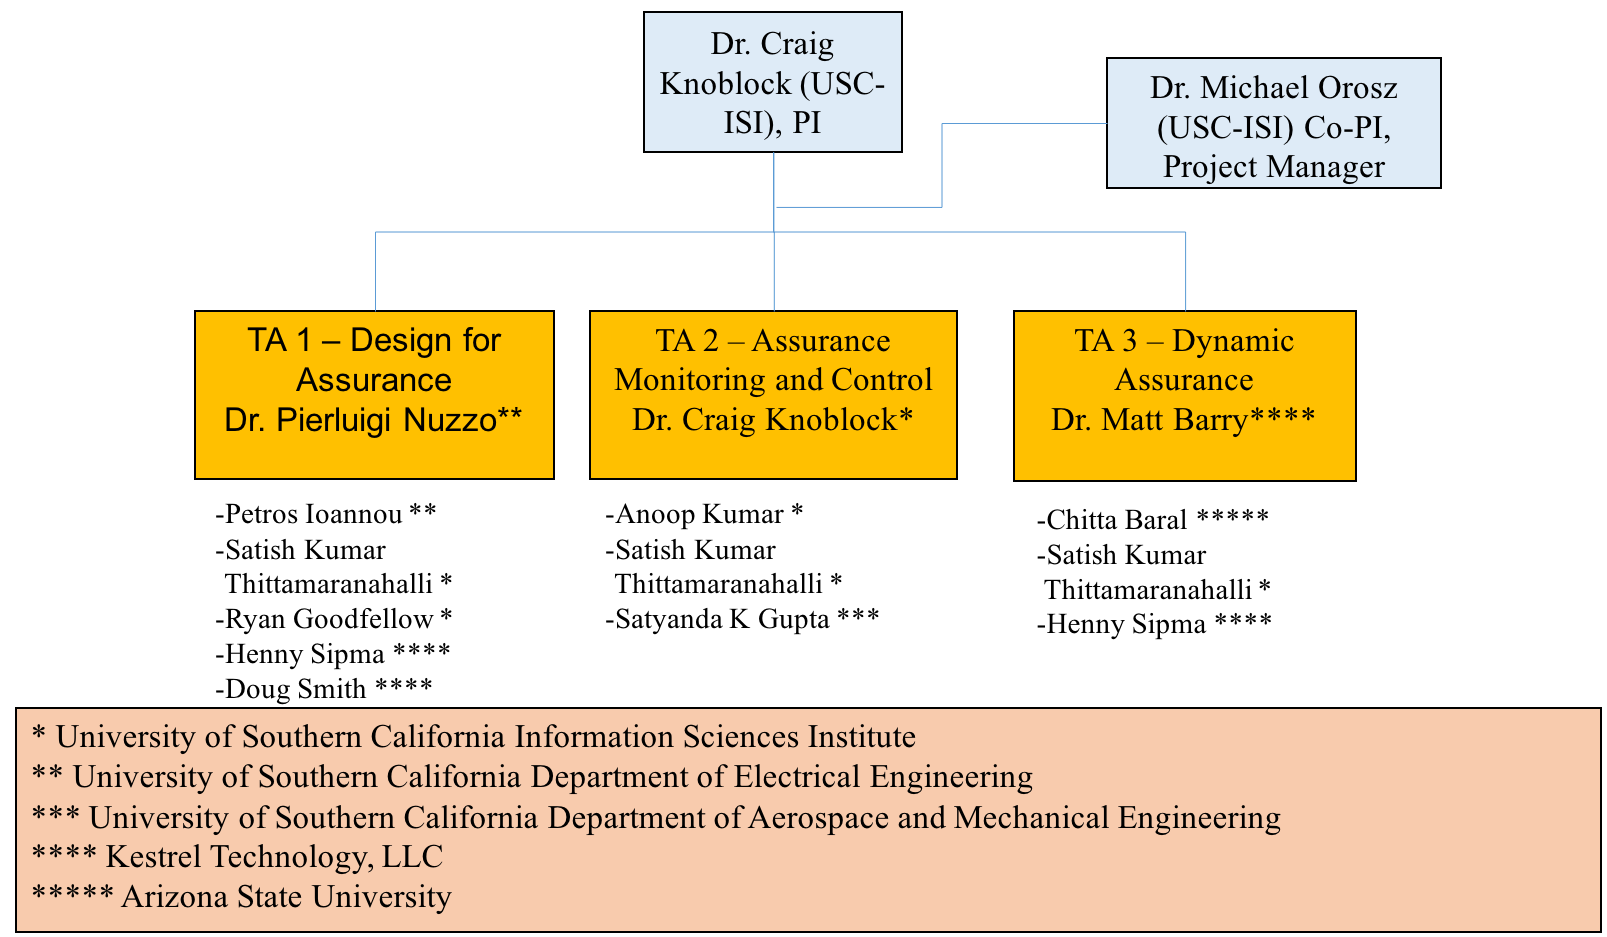
\includegraphics[width=6.0in]{./org-chart2.png}
\caption{\small Organization Chart}
\label{fig:org_chart}
\end{figure}

Coordination: To maximize collaboration and reduce risk to project failure from lack of communication and technical exchange, we plan to employ a wide variety of working styles and communication/coordination so that all can contribute.  At the core of our project will be regularly scheduled meetings bridging the diversely distributed team (Table~\ref{fig:Collaboration_Table}).  These meetings will address project status, identify challenges, implement risk mitigation strategies and participate in technology exchanges and system integration efforts (when appropriate)

\begin{table}[ht]
\caption{\small Project Meetings and Events}
  \centering
  {\footnotesize
\begin{tabular}{|m{3.15in}|m{3in}|} 
\hline
\textbf{Meeting} & \textbf{Frequency} 
\\\hline
Conference calls among investigators (discuss project status, address concerns and project risks) & Weekly
\\
\hline
Technical exchange and coordination meetings using Bluejeans or another videoconference technology & At least twice a month and more frequently as needed
  \\ 
\hline
Face-to-Face meetings (prior to P/I and demonstration meetings) & Every 3 to 6 months and more frequently (especially at the beginning of the project) as needed
 \\\cline{1-2}

\hline
\end{tabular}
}
\label{fig:Collaboration_Table}
\end{table}

\begin{table}[tbhp]
\caption{\small Key Project Team Member Responsibilities}
  \centering
  {\footnotesize
\begin{tabular}{| m{.75in} | m{3.9in}| m{1.5in}|} 
\hline
\textbf{Key Member} & \textbf{Responsibilities} & \textbf{Tasks} 
\\\hline
Dr.\ Craig Knoblock  & Principal Investigator responsible for project, leads TA 2 – Assurance Monitoring and Control.  Will lead the overall project and lead the TA2 team.  Served as the PI on many DARPA projects and has sucessfully led many large teams.    Effort on project:  25\% &
1.1.6, 1.2.2 1.2.3, 1.2.4, 1.3.4, 1.4.1, 
2.1.6, 2.2.2 2.2.3, 2.2.4, 2.3.4, 2.4.1, 
3.1.6, 3.2.2, 3.2.3, 3.2.4, 3.3.4, 3.4.1
\\
\hline
Dr.\ Michael Orosz & Co-Principal Investigator responsible managing the day-to-day operations of the project, assist technical teams as needed, coordinate with TA4 teams.    Has led many large complex multi-disciplined/multi-organizational projects in academic and industry environments.  Effort on project: 50\%
& 1.1.6, 2.1.6, 3.1.6, 1.4.1, 2.4.1, 3.4.1
  \\ 
\hline
Dr.\ Pierluigi Nuzzo 
& 
Co-Principal Investigator.  Leads the TA 1 - Design for Assurance team and conducts research on the formal methods for the design of the TA1 system.  Research experience on methodologies and tools for the design of cyber-physical systems; contracts, interfaces, and compositional methods for embedded system design; the application of automated formal methods and optimization theory to problems in embedded and cyber-physical systems.  Effort on project: 2 months/year (16.6\%)
& 
1.1.1, 2.1.1, 3.1.1 \\
\hline
Dr.\ Matthew Barry
& 
Key personnel.  Leads the TA 3 – Dynamic Assurance.   He will conduct the research on the dynamic assurance case language editors and parsers, the run-time system, and system integrations. Effort on project:  66\%
& 
1.3.2, 2.3.2, 3.3.2\\
\hline
Dr.\ Chitta Baral
& 
Key personnel responsible for learning assurance rules, supporting assurance rules with uncertainty and improving solver speed.  Expertise on ASP solvers, which will be used to reason about the assurance cases. Effort on project: 20\%
& 
1.3.1, 2.3.1, 3.3.1 \\
\hline
Dr.\ Doug Smith 
& 
Key personnel will support formal methods aspects of TA1, and lead the effort on abstract refinement. Expertise in field of automated correct-by-construction program generation.    Effort on project: 40\%
& 
1.1.5, 2.1.5, 3.1.5 \\
\hline
Dr.\ Henny Sipma
& 
Key personnel who will support the program verification tasks under TA1.  Will lead the effort on program verification.   Effort on project:  45\%
& 
1.1.5, 2.1.5, 3.1.5, 1.3.2, 2.3.2, 3.3.2 \\
\hline
Dr.\ Petros Ioannou
& 
Key personnel responsible providing and extending the assurance test bed, which will be available at the start of the project for autonomous vehicles.   Effort on project: 1 month/year (8.3\%)
& 
1.1.2, 2.1.2 (optional), 3.1.2 (optional)
\\
\hline
Dr.\ Satyandra Kumar Gupta
& 
Key Personnel providing autonomous command and control expertise to the TA-2 team.   Will lead the research on safety aware learning on TA2.   Past research on physics-aware decision making to facilitate automation.  Effort on project: 1 month/year (8.3\%)
& 
1.2.1, 2.2.1, 3.2.1 \\
\hline
Dr.\ Anoop Kumar 
& 
Key personnel providing support to the TA 2 project team.  Will lead the research on monitoring \& control and detecting distribution shifts.  Effort on project: 50\%
& 
1.2.1, 1.2.2, 1.2.3, 1.2.4, 2.2.1, 2.2.2, 2.2.3, 2.2.4, 3.2.1, 3.2.2, 3.2.3, 3.2.4\\
\hline
Dr.\ Satish Thittamaranahalli
& 
Key personnel developing scalable algorithms for TA1, TA2, and TA3 project teams.  Has extensive experience on scalable algorithm design, machine learning, and constraint reasoning.  Effort on project: 50\%
& 
1.2.1, 1.2.2, 1.2.3, 1.2.4, 2.2.1, 2.2.2, 2.2.3, 2.2.4, 3.2.1, 3.2.2, 3.2.3, 3.2.4, 1.1.4, 2.1.4, 3.1.4 \\
\hline
Dr.\ Ryan Goodfellow
& 
Key personnel providing support to the TA-1 project. Will lead the research on simulation-based testing.  Has extensive experience on simulation-based testing.  Effort on project:  30\%
& 
1.1.3, 2.1.3, 3.1.3 \\

\cline{1-2}

\hline
\end{tabular}
}
\label{fig:Table_Mgmt}
\end{table}



\newpage
\section{Personnel, Qualifications and Commitment}

{\bf Dr.\ Craig Knoblock}, the PI on this effort, is a Research Professor of both Computer Science and Spatial Sciences at the University of Southern California (USC) and Director of the Intelligent Systems Division at the USC Information Sciences Institute.   He received his Ph.D. from Carnegie Mellon University in computer science. 
%His research focuses on techniques for describing, acquiring, and exploiting the semantics of data.  
In previous projects he has worked on developing  scalable approaches to execution monitoring, accurate detection of sensor failures, and   automatic modeling and reconstruction of sensors.  He has published more than 300 journal articles, book chapters, and conference papers on these topics.  Dr. Knoblock is a Fellow of the Association for the Advancement of Artificial Intelligence (AAAI), a Distinguished Scientist of the Association of Computing Machinery (ACM), a Senior Member of IEEE, past President and Trustee of the International Joint Conference on Artificial Intelligence.
%and winner of the 2014 Robert S. Engelmore Award.  

{\bf Dr.\ Michael Orosz}, a Co-PI on this effort, is a Research Associate Professor of Civil and Environmental Engineering at the University of Southern California (USC) and Research Director of the Decision Systems Group at the USC Information Sciences Institute.  Dr. Orosz has over 30 years’ experience in commercial and government software development, basic and applied research, project management, academic research and has developed and deployed several commercially successful products.  His research interests are in machine learning and decision analytics as applied to intelligence analysis and autonomous command and control such as smart building controls.    Dr. Orosz has extensive experience in managing large complex multi-disciplined/multi-teamed research projects. %funded by DARPA, DHS, DoD, DoE, Industry, NASA, NRO, NSA and ONR.   
He received his Ph.D. in computer science from the University of California, Los Angeles.

{\bf Dr.\ Pierluigi Nuzzo}, a Co-PI on this project, is an Assistant Professor in the Department of Electrical Engineering at the University of Southern California. He received the Ph.D. in Electrical Engineering and Computer Sciences from the University of California at Berkeley. 
%in 2015, and the Laurea degree (MS) in electrical engineering (summa cum laude) from the University of Pisa, Italy, and the Sant'Anna School of Advanced Studies, Pisa, Italy.
%
%He has four years of research experience in analog and mixed signal circuit design as a researcher at IMEC, Leuven, Belgium, and over 10 years experience in design methodologies and tools for mixed-signal integrated circuits and cyber-physical systems, as a researcher at the University of Pisa, IMEC, UC Berkeley, and USC. 
His research interests
include: methodologies and tools for cyber-physical system and mixed-signal
system design; contracts, interfaces and compositional methods for embedded
system design; the application of formal methods and optimization theory to problems in embedded and cyber-physical systems and electronic design automation. 
%
Prof. Nuzzo received %First Place in the operational category and Best Overall
%Submission in the 2006 DAC/ISSCC Design Competition, 
a Marie Curie Fellowship
from the European Union in 2006, 
the University of California at Berkeley EECS
departmental fellowship in 2008, 
%the University of California at Berkeley Outstanding Graduate Student Instructor Award in 2013, 
the IBM Ph.D.
Fellowship in 2012 and 2014, 
%the Best Paper Award from the International Conference on Cyber-Physical Systems (ICCPS) in 2016, 
and the David J.~Sakrison Memorial Prize in 2016 for his doctoral research. 
%He is an author of 1 patent and over 60 publications.

{\bf Dr.\ Satyandra K. Gupta} is Smith International Professor in the Department of Aerospace and Mechanical Engineering at the University of Southern California. %Prior to joining the University of Southern California, he was a Professor in the Department of Mechanical Engineering and the Institute for Systems Research at the University of Maryland. He was the founding director of the Maryland Robotics Center and the Advanced Manufacturing Laboratory at the University of Maryland. 
He served as a program director for the National Robotics Initiative at the National Science Foundation from September 2012 to September 2014.  Dr. Gupta's interest is in the area of physics-aware decision making to facilitate automation. He has published more than 300 technical articles. He is a fellow of the American Society of Mechanical Engineers (ASME) and editor of ASME Journal of Computing and Information Science in Engineering. Dr. Gupta has received the Young Investigator Award from the Office of Naval Research in 2000, CAREER Award from the National Science Foundation in 2001, Presidential Early Career Award for Scientists and Engineers (PECASE) in 2001, Invention of the Year Award at the University of Maryland in 2007, Kos Ishii-Toshiba Award from ASME in 2011, and Excellence in Research Award from ASME in 2013.%, and Distinguished Alumnus Award from Indian Institute of Technology, Roorkee in 2014. %He has also received seven best paper awards at conferences.

{\bf Ryan Goodfellow} is a computer scientist at ISI working in combined cyber physical simulation and emulation platform development. His formal background is in simulation algorithms and modeling techniques using differential-algebraic equations (DAE). He has applied this knowledge in the CPS space by integrating DAE modeling languages and simulation engines with network testbeds to create comprehensive scientific experimentation platforms for cyber-physical systems. These experimentation platforms have been used in the power grid research space. %Ryan is a lead developer on the Deter network testbed, with a strong background in networked and distributed systems engineering. %He is also a combat veteran, serving as a non-commissioned officer and SIGINT team lead for a multi-functional intelligence team in Afghanistan.

{\bf Dr.\ Petros Ioannou} is a Professor in the Department of Electrical Engineering, Director of the Center for Advanced Transportation Technologies and Associate Director for Research for the DOT supported University Transportation Center at USC. He received his MS and PhD from the University of Illinois at Urbana Champaign in Mechanical and Electrical Engineering, respectively. His research interests are in robust adaptive control, vehicle dynamics and control, human factors and safety, automated vehicles, nonlinear systems and Intelligent transportation Systems.  He received the 2016 IEEE Transportation Technologies field award and the 2016 IEEE Control system society Transition to Practice Award. He is a Fellow of IEEE, IFAC and IET and author/coauthor of 8 books and over 400 papers.

{\bf Dr.\ Matthew Barry} will serve as lead for the TA3 tasks. %He will implement the dynamic assurance case language editors and parsers, the run-time system, and system integrations.  He will implement the assurance case arguments and the API for updating argument structure and content.  
Dr. Barry currently is CEO at Kestrel Technology LLC, and previously spent 20 years in NASA space mission operations at the Jet Propulsion Lab and Johnson Space Center.  At NASA Headquarters he led the introduction of dependability case requirements and plans for flight computing systems in upcoming manned space exploration missions, as well as the development of Agency-level software-related safety-critical control system requirements.  He recently served as a Principal Investigator on DHS/Cyber S\&T STAMP (Static Tool Analysis Modernization Program), DARPA CSFV (Crowd Sourced Formal Verification), three NASA Aeronautics R\&D projects, and the AFRL-sponsored Static Analysis of Numerical Algorithms project.  Dr. Barry earned BSME, MS, and PhD degrees in mechanical engineering, and an MBA degree, from Rice University.  

{\bf Dr.\ Henny Sipma} will support the program verification tasks under TA1.  %She is the key person behind the company's {\em KT Advance\/} and {\em KT Transferal\/} static analysis products, and the designer and programmer of the company's core {\em CodeHawk\/} abstract interpretation engine. 
Dr. Sipma currently is the CTO at Kestrel Technology LLC.  She has spent the past 10 years with Kestrel Technology as a static analysis expert; previously developed and taught static analysis techniques as senior research associate at Stanford University for eight years; and developed industrial process controls as an senior systems analyst at Shell.  She has been Principal Investigator or company lead on several recent R\&D projects for Federal agencies, including two projects under the IARPA STONESOUP (Securely Taking On New Executable Software of Uncertain Provenance) program; the DHS Cyber S\&T Gold Standard project; and the DARPA-sponsored STAC (Space-Time Analysis for Cybersecurity) and MUSE (Mining and Understanding Software Enclaves) programs.  Dr. Sipma earned 
%a BS degree in chemistry and an MS degree in chemical engineering at the University of Groningen in The Netherlands, and 
MS and PhD degrees in computer science from Stanford University.  

{\bf Dr.\ Douglas R.\ Smith} will support formal methods aspects of TA1, including the enforcement of safety properties and the generation of monitors.  He is President of Kestrel Technology LLC and Principal Scientist at Kestrel Institute.  He is a Fellow of the American Association of Artificial Intelligence (AAAI) and an ASE Fellow (Automated Software Engineering).  From 1986 to 2000, he taught an advanced graduate course on correct-by-construction software development at Stanford.  
%Dr. Smith has led the development of a series of software synthesis systems, including KIDS (Kestrel Interactive Development System), Specware, Designware, and Planware. 
%Applications domains have included a variety of complex high-performance planners and schedulers for the US Air Force.  He leads current projects on the generation of air mission plans and cyberoperations.  
Other recent projects focused on automated policy enforcement \cite{SmithD0703,SmithD08}, synthesis of secure network protocol codes, and the synthesis of high-performance constraint-solvers\cite{SmithD08c,SmithD13}.  Dr. Smith has over 30 years experience in the field of automated correct-by-construction program generation and has published over 100 papers. He has one patent.  He received the Ph.D. in Computer Science from Duke University% in 1979.  

{\bf Dr. Chitta Baral} is a Professor in the Department of Computer Science and Engineering at Arizona State University. He will support the TA3 efforts on Learning assurance rules, supporting assurance rules with uncertainty and improving solver speed. Dr. Baral has expertise in various aspects of autonomy and Artificial Intelligence. 
He wrote the first book on answer set programming (published by Cambridge University Press) the formal language behind our assurance rules. Some of his other works relevant to this proposal are: goal specification for autonomous systems, automatic construction of control rules for autonomous systems that satisfy given goals, combining machine learning with reasoning in various contexts, including image understanding. %He is the President of KR Inc. He is an associate editor of AIJ and has been an associate editor of JAIR.

{\bf Dr.\ Satish Kumar Thittamaranahalli (T. K. Satish Kumar)} leads the Collaboratory for Algorithmic Techniques and Artificial Intelligence (CATAI) at USC's Information Sciences Institute. He has published over 60 papers on numerous topics in Artificial Intelligence spanning such diverse areas as Constraint Reasoning, Planning and Scheduling, Probabilistic Reasoning, Robotics, Combinatorial Optimization, Approximation and Randomization, Heuristic Search, Model-Based Reasoning, Knowledge Representation and Spatio-Temporal Reasoning. %He %has served on the Program Committees of many international conferences in Artificial Intelligence
He and is a winner of the 2016 Best Robotics Paper Award and the 2005 Best Student Paper Award from the International Conference on Automated Planning and Scheduling. 
Dr. Kumar received his PhD in Computer Science from Stanford University. %In the past, he has also been a Visiting Student at the NASA Ames Research Center, a Postdoctoral Research Scholar at the University of California, Berkeley, a Research Scientist at the Institute for Human and Machine Cognition, a Visiting Assistant Professor at the University of West Florida, and a Senior Research and Development Scientist at Mission Critical Technologies.

\textbf{Dr.\ Anoop Kumar} is a senior computer scientist at USC ISI and has broad expertise in machine learning, statistical modeling, and software engineering.  Dr.\ Kumar is the technical lead on the DARPA RSPACE program and has played a vital role in developing a system that fuses air operations data from multiple sources, maintains world state, and issues warnings. Previously, he led the research and development of the BBN’s election forecasting system for the IARPA OSI program. %Dr.\ Kumar played a significant role in the DARPA DEFT program by developing a model to support integration of output from multiple NLP algorithms. He has contributed at the development to management levels on government research contracts and commercial projects. 
Dr.\ Kumar helped design and develop BBN's commercially available, hosted speech and medical transcription services offering. 

\begin{table}[!tbh]
\begin{footnotesize}
\vspace{-0.1in}

\begin{tabular}{lll}
\begin{tabular}[t]{|l|@{}c@{}|@{}c@{}|@{}c@{}|@{}c@{}|} \hline
Project & Status & \multicolumn{3}{ c| }{Hours} \\ \cline{3-5}
& & P1 & P2 & P3 \\ \hline



\multicolumn{5}{ |c| }{ \textbf{Craig Knoblock} } \\ \cline{1-5}
Safeguard & Pro & 770 & 641 & 641 \\ \cline{1-5}
ELICIT & Cur & 308 & 256 & 120 \\ \cline{1-5}
WTNIC & Cur & 11 & 0 & 0 \\ \cline{1-5}
EFFECT & Cur & 641 & 107 & 0 \\ \cline{1-5}
LinkedMaps & Cur & 203 & 25 & 0 \\ \cline{1-5}
PRINCESS & Cur & 608 & 96 & 0 \\ \cline{1-5}
SCHARP & Cur & 481 & 54 & 0 \\ \cline{1-5}
MINT & Pen & 650 & 534 & 285 \\ \cline{1-5}

\multicolumn{5}{ |c| }{ \textbf{Michael Orosz} } \\ \cline{1-5}
Safeguard & Pro & 1560 & 1300 & 1300  \\ \cline{1-5}
SMC/SY & Cur & 1803 & 0 & 0  \\ \cline{1-5}

\multicolumn{5}{ |c| }{ \textbf{Matthew Barry} } \\ \cline{1-5}
Safeguard & Pro & 2078 & 1690 & 1554 \\ \cline{1-5}
Starlite & Cur & 1840 & 1692 & 0 \\ \cline{1-5}



\multicolumn{5}{ |c| }{ \textbf{Anoop Kumar} } \\ \cline{1-5}
Safeguard & Pro & 1560 & 1300 & 1300 \\ \cline{1-5}

\end{tabular}
&
\begin{tabular}[t]{|l|@{}c@{}|@{}c@{}|@{}c@{}|@{}c@{}|} \hline
Project & Status & \multicolumn{3}{ c| }{Hours} \\ \cline{3-5}
& & P1 & P2 & P3 \\ \hline

\multicolumn{5}{ |c| }{ \textbf{Pierluigi Nuzzo} } \\ \cline{1-5}
Safeguard & Pro & 520 & 433 & 433  \\ \cline{1-5}
Mirage & Cur & 433 & 0 & 0  \\ \cline{1-5}

\multicolumn{5}{ |c| }{ \textbf{Satyandra Gupta} } \\ \cline{1-5}
Safeguard & Pro & 260 & 217 & 217 \\ \cline{1-5}
Human   & Cur & 22 & 0 & 0 \\ \cline{1-5}
Vehicles & Cur & 36 & 0 & 0 \\ \cline{1-5}
Robot & Cur & 116 & 0 & 0 \\ \cline{1-5}
Assembly & Cur & 33 & 0 & 0 \\ \cline{1-5}
Solar & Cur & 4 & 0 & 0 \\ \cline{1-5}

\multicolumn{5}{ |c| }{ \textbf{Petros Ioannou} } \\ \cline{1-5}
Safeguard & Pro & 260 & 217 & 217 \\ \cline{1-5}
CPS & Cur & 130 & 0 & 0 \\ \cline{1-5}

\multicolumn{5}{ |c| }{ \textbf{Ryan Goodfellow} } \\ \cline{1-5}
Safeguard & Pro & 936 & 780 & 780 \\ \cline{1-5}
STEAM & Cur & 416 & 0 & 0 \\ \cline{1-5}


\end{tabular}
&
\begin{tabular}[t]{|l|@{}c@{}|@{}c@{}|@{}c@{}|@{}c@{}|} \hline
Project & Status & \multicolumn{3}{ c| }{Hours} \\ \cline{3-5}
& & P1 & P2 & P3 \\ \hline

\multicolumn{5}{ |c| }{ \textbf{Chitta Baral} } \\ \cline{1-5}
Safeguard & Pro & 659 & 485 & 485 \\ \cline{1-5}
PostdocBP & Cur & 176 & 0 & 0 \\ \cline{1-5}
Languages & Pen & 528 & 264 & 264 \\ \cline{1-5}
CAREER & Pen & 88 & 44 & 44 \\ \cline{1-5}
CHS & Pen & 510 & 255 & 0 \\ \cline{1-5}

\multicolumn{5}{ |c| }{ \textbf{Doug Smith} } \\ \cline{1-5}
Safeguard & Pro & 1222 & 984 & 840 \\ \cline{1-5}
RSPACE & Cur & 342 & 0 & 0 \\ 
\cline{1-5}
PLANX & Cur & 154 & 0 & 0 \\ 
\cline{1-5}
HACCS & Pen & 923 & 769 & 769 \\ 
\cline{1-5}

\multicolumn{5}{ |c| }{ \textbf{Henny Sipma} } \\ \cline{1-5}
Safeguard & Pro & 1372 & 962 & 840 \\ \cline{1-5}
STAC & Cur & 797 & 0 & 0 \\ \cline{1-5}

\multicolumn{5}{ |c| }{ \textbf{Satish Thittamaranahalli} } \\ \cline{1-5}
Safeguard & Pro & 1560 & 1300 & 1300 \\ \cline{1-5}
MapF & Cur & 103 & 103 & 0 \\ \cline{1-5}

\end{tabular}
\end{tabular}

\end{footnotesize}
\caption{Individual commitments of key personnel}
\label{tab:Commitments}
\vspace{-0.2in}
\end{table}

\clearpage
\newpage
\section{Capabilities}


%\subsection{University of Southern California}
USC has strengths in number of areas that are closely related to the proposed work:
\begin{itemize}[itemsep=0pt,leftmargin=*]
\item Dr.\ Nuzzo 
%has over 10-year research experience in embedded system design, from mixed-signal chip design (analog-to-digital converters, frequency synthesizers, software-defined radio), to methodologies and tools for mixed-signal integrated circuits and Cyber-Physical Systems (CPSs), and the application of formal methods and optimization theory to problems in embedded and cyber-physical systems and electronic design automation.  
%His doctoral work 
has done extensive research on contracts and compositional methods for heterogeneous system design and design space exploration, with application to aircraft electric power systems and environmental control systems. His work has helped transition rigorous system design foundations, innovative design methodologies, and new systems engineering paradigms to industry (IBM, United Technologies). 
\item Dr.\ Satyandra K. Gupta has worked on autonomous surface vehicles, autonomous ground vehicles for operation on rugged terrains, and autonomous flapping wing aerial vehicles.   His group has developed a hierarchal decision making approach for realizing autonomous systems. 
%This approach combines task planning and assignment, deliberative trajectory planning, reactive collision avoidance behaviors, and trajectory tracking control layers. 
His group has also developed new methods for learning reactive behaviors in adversarial environments and COLREGS compliant trajectory planning. \item Dr.\ Knoblock has developed methods that learn the relationships between sensors to both identify failures and changes in sensor and reconstruct those sensors, providing estimates of the accuracy of the reconstructed sensors.  
\item Ryan Goodfellow has extensive experience in simulation based testing through high-fidelity CPS testbed environment development and operation, using the Deter network testbed as the core which has supported several large scale government projects from a variety of agencies and thousands of users. %we have developed sophisticated CPS experiments under programs such as NFS RIPS, NIST SmartCities and the DHS Cybersecurity showcase.
\item Dr.\ Ioannou %helped  design and implement adaptive cruise control systems in collaboration with Ford Motor Company, which was commercialized four years before any other company. He 
worked on several DOT funded projects on automated vehicles and intelligent highway systems where he demonstrated his vehicle control designs for safety and performance on actual automated vehicles in test trucks and I-15 highway.
\item Drs.\ Knoblock, Kumar, and Thittamaranahalli have developed highly scalable approaches for monitoring message traffic to identify potential problems and issue warnings and alerts. 
\item Dr. Thittamaranahalli has developed state-of-the-art methods for efficiently solving large-scale search and optimization problems. %These techniques will be applicable in TA2 for safety-aware learning and planning, in TA2 for assurance monitoring and control, and in TA3 for dynamic assessment of assurance cases.

\end{itemize}
%\subsection{Kestrel Technology LLC}

Kestrel Technology's strength is in program analysis, specifically static analysis of both source and binary targets.  The company performs applied R\&D and product development for a variety of static analysis applications  pivoting primarily on the abstract interpretation technique.  The company recently initiated development of program analysis applications using logical equivalence techniques. As a provider of verification evidence in the form of mathematical proofs, the company also has expertise in the design and development of assurance case arguments for high-integrity systems using such evidence. %The company is engaged in a partnership with Wind River Systems to develop program analysis tools for its embedded system developers.  Many of Wind River's customers must develop their products under safety and certification standards, including those using safety cases.  

   

%\subsection{Arizona State University}
Chitta Baral at Arizona State University has developed various software to learn assurance rules and various ASP solvers, which he has made available as open-source.

Most of the software carried forward for implementation or derivation is open source.  The single exception is Kestrel Technology's {\it KT Advance\/} static analysis tool (TA1), in particular the abstract interpretation engine therein, which is company proprietary and is US EAR export-controlled.   
%Owing to mixed funding for the development of that technology 
We will continue to provide the Federal government a restricted use license for that particular item.

There are no specialized facilities, data, or GFE required for this effort. 

\include{sow}
\include{milestones}

% \section{Level of Effort by Task \textcolor{red}{[Mike/Lisa - 1 pages]}}

% \textcolor{blue}{
% \begin{itemize}
% \item Will be a separate spreadsheet
% \item
% \end{itemize}
% }

\include{appendix_a}

%\section{Appendix B \textcolor{red}{[No Page Count]}}

\section{References}
\bibliographystyle{acm} 
\bibliography{TA3/ta3,TA2/ta2,TA1/ta1}
\end{document}
\clearpage
\newpage


\section{Management Plan}


The Principal Investigator for this effort is Dr. Craig Knoblock who is responsible for all aspects of the effort, will coordinate the parallel team efforts, and will ensure high levels of performance from individual team members.  The Co-P/I, Dr. Michael Orosz, will provide project management and will assist all performers in the execution of the project.    The project team is divided into three working groups (Figure~\ref{fig:org_chart}) corresponding to Technical Areas 1-3, however, members of each team contribute across all project activities.   Table~\ref{fig:Table_Mgmt} defines the major contributions of each project team member to the project tasks.

\begin{figure}[tbhp]
%\vspace{-25pt}
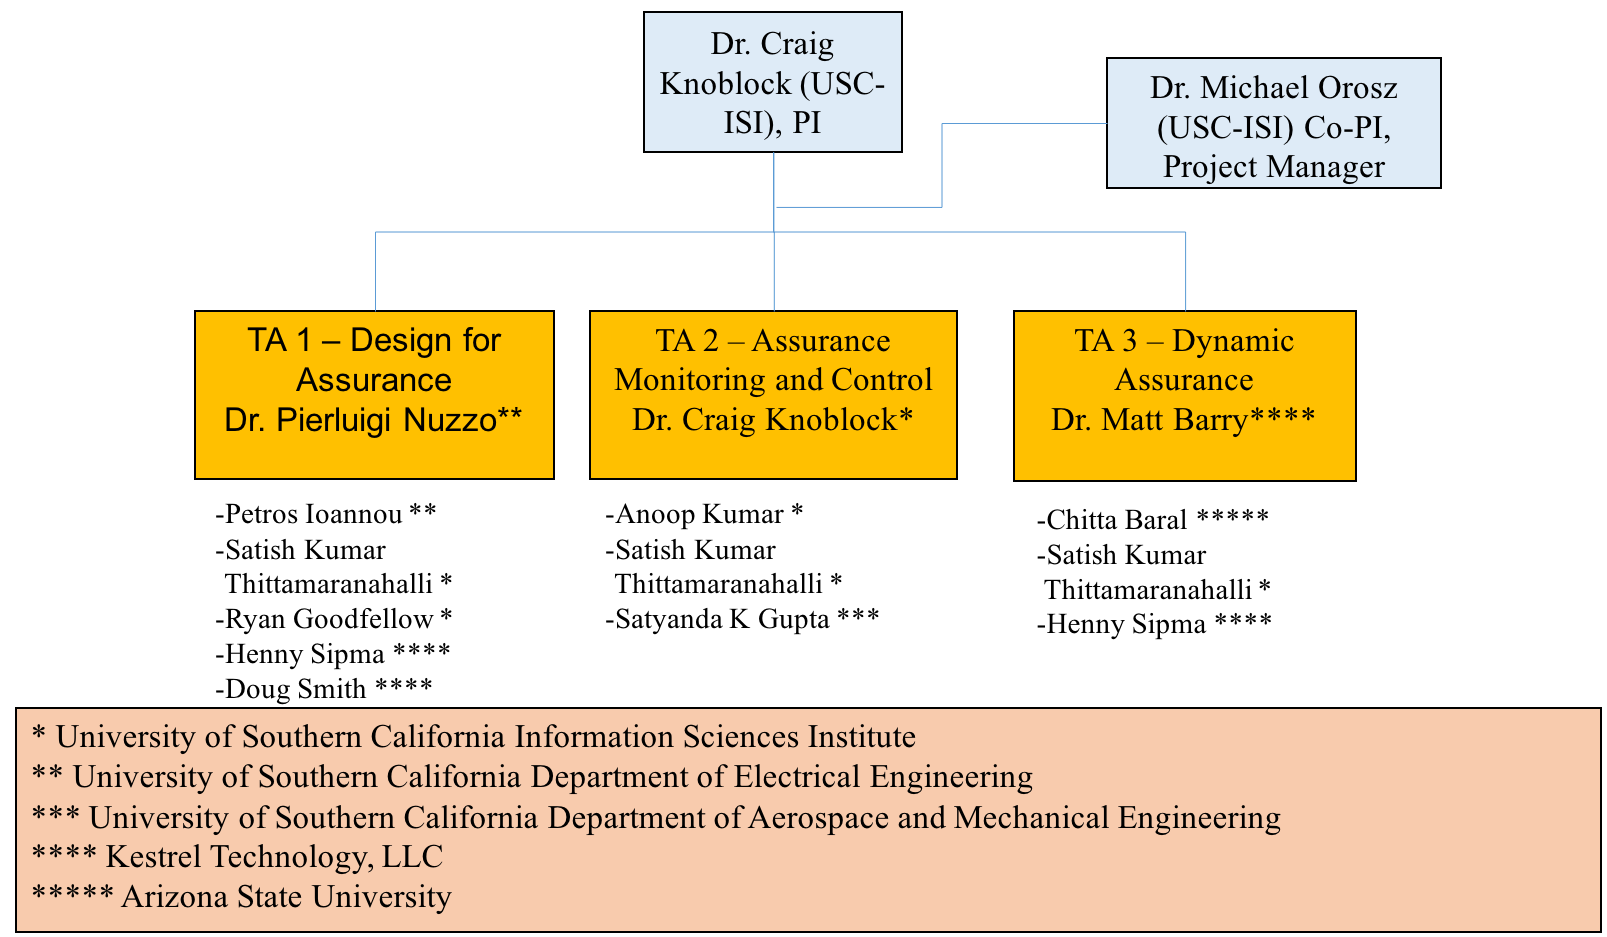
\includegraphics[width=6.0in]{./org-chart2.png}
\caption{\small Organization Chart}
\label{fig:org_chart}
\end{figure}

Coordination: To maximize collaboration and reduce risk to project failure from lack of communication and technical exchange, we plan to employ a wide variety of working styles and communication/coordination so that all can contribute.  At the core of our project will be regularly scheduled meetings bridging the diversely distributed team (Table~\ref{fig:Collaboration_Table}).  These meetings will address project status, identify challenges, implement risk mitigation strategies and participate in technology exchanges and system integration efforts (when appropriate)

\begin{table}[ht]
\caption{\small Project Meetings and Events}
  \centering
  {\footnotesize
\begin{tabular}{|m{3.15in}|m{3in}|} 
\hline
\textbf{Meeting} & \textbf{Frequency} 
\\\hline
Conference calls among investigators (discuss project status, address concerns and project risks) & Weekly
\\
\hline
Technical exchange and coordination meetings using Bluejeans or another videoconference technology & At least twice a month and more frequently as needed
  \\ 
\hline
Face-to-Face meetings (prior to P/I and demonstration meetings) & Every 3 to 6 months and more frequently (especially at the beginning of the project) as needed
 \\\cline{1-2}

\hline
\end{tabular}
}
\label{fig:Collaboration_Table}
\end{table}

\begin{table}[tbhp]
\caption{\small Key Project Team Member Responsibilities}
  \centering
  {\footnotesize
\begin{tabular}{| m{.75in} | m{3.9in}| m{1.5in}|} 
\hline
\textbf{Key Member} & \textbf{Responsibilities} & \textbf{Tasks} 
\\\hline
Dr.\ Craig Knoblock  & Principal Investigator responsible for project, leads TA 2 – Assurance Monitoring and Control.  Will lead the overall project and lead the TA2 team.  Served as the PI on many DARPA projects and has sucessfully led many large teams.    Effort on project:  25\% &
1.1.6, 1.2.2 1.2.3, 1.2.4, 1.3.4, 1.4.1, 
2.1.6, 2.2.2 2.2.3, 2.2.4, 2.3.4, 2.4.1, 
3.1.6, 3.2.2, 3.2.3, 3.2.4, 3.3.4, 3.4.1
\\
\hline
Dr.\ Michael Orosz & Co-Principal Investigator responsible managing the day-to-day operations of the project, assist technical teams as needed, coordinate with TA4 teams.    Has led many large complex multi-disciplined/multi-organizational projects in academic and industry environments.  Effort on project: 50\%
& 1.1.6, 2.1.6, 3.1.6, 1.4.1, 2.4.1, 3.4.1
  \\ 
\hline
Dr.\ Pierluigi Nuzzo 
& 
Co-Principal Investigator.  Leads the TA 1 - Design for Assurance team and conducts research on the formal methods for the design of the TA1 system.  Research experience on methodologies and tools for the design of cyber-physical systems; contracts, interfaces, and compositional methods for embedded system design; the application of automated formal methods and optimization theory to problems in embedded and cyber-physical systems.  Effort on project: 2 months/year (16.6\%)
& 
1.1.1, 2.1.1, 3.1.1 \\
\hline
Dr.\ Matthew Barry
& 
Key personnel.  Leads the TA 3 – Dynamic Assurance.   He will conduct the research on the dynamic assurance case language editors and parsers, the run-time system, and system integrations. Effort on project:  66\%
& 
1.3.2, 2.3.2, 3.3.2\\
\hline
Dr.\ Chitta Baral
& 
Key personnel responsible for learning assurance rules, supporting assurance rules with uncertainty and improving solver speed.  Expertise on ASP solvers, which will be used to reason about the assurance cases. Effort on project: 20\%
& 
1.3.1, 2.3.1, 3.3.1 \\
\hline
Dr.\ Doug Smith 
& 
Key personnel will support formal methods aspects of TA1, and lead the effort on abstract refinement. Expertise in field of automated correct-by-construction program generation.    Effort on project: 40\%
& 
1.1.5, 2.1.5, 3.1.5 \\
\hline
Dr.\ Henny Sipma
& 
Key personnel who will support the program verification tasks under TA1.  Will lead the effort on program verification.   Effort on project:  45\%
& 
1.1.5, 2.1.5, 3.1.5, 1.3.2, 2.3.2, 3.3.2 \\
\hline
Dr.\ Petros Ioannou
& 
Key personnel responsible providing and extending the assurance test bed, which will be available at the start of the project for autonomous vehicles.   Effort on project: 1 month/year (8.3\%)
& 
1.1.2, 2.1.2 (optional), 3.1.2 (optional)
\\
\hline
Dr.\ Satyandra Kumar Gupta
& 
Key Personnel providing autonomous command and control expertise to the TA-2 team.   Will lead the research on safety aware learning on TA2.   Past research on physics-aware decision making to facilitate automation.  Effort on project: 1 month/year (8.3\%)
& 
1.2.1, 2.2.1, 3.2.1 \\
\hline
Dr.\ Anoop Kumar 
& 
Key personnel providing support to the TA 2 project team.  Will lead the research on monitoring \& control and detecting distribution shifts.  Effort on project: 50\%
& 
1.2.1, 1.2.2, 1.2.3, 1.2.4, 2.2.1, 2.2.2, 2.2.3, 2.2.4, 3.2.1, 3.2.2, 3.2.3, 3.2.4\\
\hline
Dr.\ Satish Thittamaranahalli
& 
Key personnel developing scalable algorithms for TA1, TA2, and TA3 project teams.  Has extensive experience on scalable algorithm design, machine learning, and constraint reasoning.  Effort on project: 50\%
& 
1.2.1, 1.2.2, 1.2.3, 1.2.4, 2.2.1, 2.2.2, 2.2.3, 2.2.4, 3.2.1, 3.2.2, 3.2.3, 3.2.4, 1.1.4, 2.1.4, 3.1.4 \\
\hline
Dr.\ Ryan Goodfellow
& 
Key personnel providing support to the TA-1 project. Will lead the research on simulation-based testing.  Has extensive experience on simulation-based testing.  Effort on project:  30\%
& 
1.1.3, 2.1.3, 3.1.3 \\

\cline{1-2}

\hline
\end{tabular}
}
\label{fig:Table_Mgmt}
\end{table}



\newpage
\section{Personnel, Qualifications and Commitment}

{\bf Dr.\ Craig Knoblock}, the PI on this effort, is a Research Professor of both Computer Science and Spatial Sciences at the University of Southern California (USC) and Director of the Intelligent Systems Division at the USC Information Sciences Institute.   He received his Ph.D. from Carnegie Mellon University in computer science. 
%His research focuses on techniques for describing, acquiring, and exploiting the semantics of data.  
In previous projects he has worked on developing  scalable approaches to execution monitoring, accurate detection of sensor failures, and   automatic modeling and reconstruction of sensors.  He has published more than 300 journal articles, book chapters, and conference papers on these topics.  Dr. Knoblock is a Fellow of the Association for the Advancement of Artificial Intelligence (AAAI), a Distinguished Scientist of the Association of Computing Machinery (ACM), a Senior Member of IEEE, past President and Trustee of the International Joint Conference on Artificial Intelligence.
%and winner of the 2014 Robert S. Engelmore Award.  

{\bf Dr.\ Michael Orosz}, a Co-PI on this effort, is a Research Associate Professor of Civil and Environmental Engineering at the University of Southern California (USC) and Research Director of the Decision Systems Group at the USC Information Sciences Institute.  Dr. Orosz has over 30 years’ experience in commercial and government software development, basic and applied research, project management, academic research and has developed and deployed several commercially successful products.  His research interests are in machine learning and decision analytics as applied to intelligence analysis and autonomous command and control such as smart building controls.    Dr. Orosz has extensive experience in managing large complex multi-disciplined/multi-teamed research projects. %funded by DARPA, DHS, DoD, DoE, Industry, NASA, NRO, NSA and ONR.   
He received his Ph.D. in computer science from the University of California, Los Angeles.

{\bf Dr.\ Pierluigi Nuzzo}, a Co-PI on this project, is an Assistant Professor in the Department of Electrical Engineering at the University of Southern California. He received the Ph.D. in Electrical Engineering and Computer Sciences from the University of California at Berkeley. 
%in 2015, and the Laurea degree (MS) in electrical engineering (summa cum laude) from the University of Pisa, Italy, and the Sant'Anna School of Advanced Studies, Pisa, Italy.
%
%He has four years of research experience in analog and mixed signal circuit design as a researcher at IMEC, Leuven, Belgium, and over 10 years experience in design methodologies and tools for mixed-signal integrated circuits and cyber-physical systems, as a researcher at the University of Pisa, IMEC, UC Berkeley, and USC. 
His research interests
include: methodologies and tools for cyber-physical system and mixed-signal
system design; contracts, interfaces and compositional methods for embedded
system design; the application of formal methods and optimization theory to problems in embedded and cyber-physical systems and electronic design automation. 
%
Prof. Nuzzo received %First Place in the operational category and Best Overall
%Submission in the 2006 DAC/ISSCC Design Competition, 
a Marie Curie Fellowship
from the European Union in 2006, 
the University of California at Berkeley EECS
departmental fellowship in 2008, 
%the University of California at Berkeley Outstanding Graduate Student Instructor Award in 2013, 
the IBM Ph.D.
Fellowship in 2012 and 2014, 
%the Best Paper Award from the International Conference on Cyber-Physical Systems (ICCPS) in 2016, 
and the David J.~Sakrison Memorial Prize in 2016 for his doctoral research. 
%He is an author of 1 patent and over 60 publications.

{\bf Dr.\ Satyandra K. Gupta} is Smith International Professor in the Department of Aerospace and Mechanical Engineering at the University of Southern California. %Prior to joining the University of Southern California, he was a Professor in the Department of Mechanical Engineering and the Institute for Systems Research at the University of Maryland. He was the founding director of the Maryland Robotics Center and the Advanced Manufacturing Laboratory at the University of Maryland. 
He served as a program director for the National Robotics Initiative at the National Science Foundation from September 2012 to September 2014.  Dr. Gupta's interest is in the area of physics-aware decision making to facilitate automation. He has published more than 300 technical articles. He is a fellow of the American Society of Mechanical Engineers (ASME) and editor of ASME Journal of Computing and Information Science in Engineering. Dr. Gupta has received the Young Investigator Award from the Office of Naval Research in 2000, CAREER Award from the National Science Foundation in 2001, Presidential Early Career Award for Scientists and Engineers (PECASE) in 2001, Invention of the Year Award at the University of Maryland in 2007, Kos Ishii-Toshiba Award from ASME in 2011, and Excellence in Research Award from ASME in 2013.%, and Distinguished Alumnus Award from Indian Institute of Technology, Roorkee in 2014. %He has also received seven best paper awards at conferences.

{\bf Ryan Goodfellow} is a computer scientist at ISI working in combined cyber physical simulation and emulation platform development. His formal background is in simulation algorithms and modeling techniques using differential-algebraic equations (DAE). He has applied this knowledge in the CPS space by integrating DAE modeling languages and simulation engines with network testbeds to create comprehensive scientific experimentation platforms for cyber-physical systems. These experimentation platforms have been used in the power grid research space. %Ryan is a lead developer on the Deter network testbed, with a strong background in networked and distributed systems engineering. %He is also a combat veteran, serving as a non-commissioned officer and SIGINT team lead for a multi-functional intelligence team in Afghanistan.

{\bf Dr.\ Petros Ioannou} is a Professor in the Department of Electrical Engineering, Director of the Center for Advanced Transportation Technologies and Associate Director for Research for the DOT supported University Transportation Center at USC. He received his MS and PhD from the University of Illinois at Urbana Champaign in Mechanical and Electrical Engineering, respectively. His research interests are in robust adaptive control, vehicle dynamics and control, human factors and safety, automated vehicles, nonlinear systems and Intelligent transportation Systems.  He received the 2016 IEEE Transportation Technologies field award and the 2016 IEEE Control system society Transition to Practice Award. He is a Fellow of IEEE, IFAC and IET and author/coauthor of 8 books and over 400 papers.

{\bf Dr.\ Matthew Barry} will serve as lead for the TA3 tasks. %He will implement the dynamic assurance case language editors and parsers, the run-time system, and system integrations.  He will implement the assurance case arguments and the API for updating argument structure and content.  
Dr. Barry currently is CEO at Kestrel Technology LLC, and previously spent 20 years in NASA space mission operations at the Jet Propulsion Lab and Johnson Space Center.  At NASA Headquarters he led the introduction of dependability case requirements and plans for flight computing systems in upcoming manned space exploration missions, as well as the development of Agency-level software-related safety-critical control system requirements.  He recently served as a Principal Investigator on DHS/Cyber S\&T STAMP (Static Tool Analysis Modernization Program), DARPA CSFV (Crowd Sourced Formal Verification), three NASA Aeronautics R\&D projects, and the AFRL-sponsored Static Analysis of Numerical Algorithms project.  Dr. Barry earned BSME, MS, and PhD degrees in mechanical engineering, and an MBA degree, from Rice University.  

{\bf Dr.\ Henny Sipma} will support the program verification tasks under TA1.  %She is the key person behind the company's {\em KT Advance\/} and {\em KT Transferal\/} static analysis products, and the designer and programmer of the company's core {\em CodeHawk\/} abstract interpretation engine. 
Dr. Sipma currently is the CTO at Kestrel Technology LLC.  She has spent the past 10 years with Kestrel Technology as a static analysis expert; previously developed and taught static analysis techniques as senior research associate at Stanford University for eight years; and developed industrial process controls as an senior systems analyst at Shell.  She has been Principal Investigator or company lead on several recent R\&D projects for Federal agencies, including two projects under the IARPA STONESOUP (Securely Taking On New Executable Software of Uncertain Provenance) program; the DHS Cyber S\&T Gold Standard project; and the DARPA-sponsored STAC (Space-Time Analysis for Cybersecurity) and MUSE (Mining and Understanding Software Enclaves) programs.  Dr. Sipma earned 
%a BS degree in chemistry and an MS degree in chemical engineering at the University of Groningen in The Netherlands, and 
MS and PhD degrees in computer science from Stanford University.  

{\bf Dr.\ Douglas R.\ Smith} will support formal methods aspects of TA1, including the enforcement of safety properties and the generation of monitors.  He is President of Kestrel Technology LLC and Principal Scientist at Kestrel Institute.  He is a Fellow of the American Association of Artificial Intelligence (AAAI) and an ASE Fellow (Automated Software Engineering).  From 1986 to 2000, he taught an advanced graduate course on correct-by-construction software development at Stanford.  
%Dr. Smith has led the development of a series of software synthesis systems, including KIDS (Kestrel Interactive Development System), Specware, Designware, and Planware. 
%Applications domains have included a variety of complex high-performance planners and schedulers for the US Air Force.  He leads current projects on the generation of air mission plans and cyberoperations.  
Other recent projects focused on automated policy enforcement \cite{SmithD0703,SmithD08}, synthesis of secure network protocol codes, and the synthesis of high-performance constraint-solvers\cite{SmithD08c,SmithD13}.  Dr. Smith has over 30 years experience in the field of automated correct-by-construction program generation and has published over 100 papers. He has one patent.  He received the Ph.D. in Computer Science from Duke University% in 1979.  

{\bf Dr. Chitta Baral} is a Professor in the Department of Computer Science and Engineering at Arizona State University. He will support the TA3 efforts on Learning assurance rules, supporting assurance rules with uncertainty and improving solver speed. Dr. Baral has expertise in various aspects of autonomy and Artificial Intelligence. 
He wrote the first book on answer set programming (published by Cambridge University Press) the formal language behind our assurance rules. Some of his other works relevant to this proposal are: goal specification for autonomous systems, automatic construction of control rules for autonomous systems that satisfy given goals, combining machine learning with reasoning in various contexts, including image understanding. %He is the President of KR Inc. He is an associate editor of AIJ and has been an associate editor of JAIR.

{\bf Dr.\ Satish Kumar Thittamaranahalli (T. K. Satish Kumar)} leads the Collaboratory for Algorithmic Techniques and Artificial Intelligence (CATAI) at USC's Information Sciences Institute. He has published over 60 papers on numerous topics in Artificial Intelligence spanning such diverse areas as Constraint Reasoning, Planning and Scheduling, Probabilistic Reasoning, Robotics, Combinatorial Optimization, Approximation and Randomization, Heuristic Search, Model-Based Reasoning, Knowledge Representation and Spatio-Temporal Reasoning. %He %has served on the Program Committees of many international conferences in Artificial Intelligence
He and is a winner of the 2016 Best Robotics Paper Award and the 2005 Best Student Paper Award from the International Conference on Automated Planning and Scheduling. 
Dr. Kumar received his PhD in Computer Science from Stanford University. %In the past, he has also been a Visiting Student at the NASA Ames Research Center, a Postdoctoral Research Scholar at the University of California, Berkeley, a Research Scientist at the Institute for Human and Machine Cognition, a Visiting Assistant Professor at the University of West Florida, and a Senior Research and Development Scientist at Mission Critical Technologies.

\textbf{Dr.\ Anoop Kumar} is a senior computer scientist at USC ISI and has broad expertise in machine learning, statistical modeling, and software engineering.  Dr.\ Kumar is the technical lead on the DARPA RSPACE program and has played a vital role in developing a system that fuses air operations data from multiple sources, maintains world state, and issues warnings. Previously, he led the research and development of the BBN’s election forecasting system for the IARPA OSI program. %Dr.\ Kumar played a significant role in the DARPA DEFT program by developing a model to support integration of output from multiple NLP algorithms. He has contributed at the development to management levels on government research contracts and commercial projects. 
Dr.\ Kumar helped design and develop BBN's commercially available, hosted speech and medical transcription services offering. 

\begin{table}[!tbh]
\begin{footnotesize}
\vspace{-0.1in}

\begin{tabular}{lll}
\begin{tabular}[t]{|l|@{}c@{}|@{}c@{}|@{}c@{}|@{}c@{}|} \hline
Project & Status & \multicolumn{3}{ c| }{Hours} \\ \cline{3-5}
& & P1 & P2 & P3 \\ \hline



\multicolumn{5}{ |c| }{ \textbf{Craig Knoblock} } \\ \cline{1-5}
Safeguard & Pro & 770 & 641 & 641 \\ \cline{1-5}
ELICIT & Cur & 308 & 256 & 120 \\ \cline{1-5}
WTNIC & Cur & 11 & 0 & 0 \\ \cline{1-5}
EFFECT & Cur & 641 & 107 & 0 \\ \cline{1-5}
LinkedMaps & Cur & 203 & 25 & 0 \\ \cline{1-5}
PRINCESS & Cur & 608 & 96 & 0 \\ \cline{1-5}
SCHARP & Cur & 481 & 54 & 0 \\ \cline{1-5}
MINT & Pen & 650 & 534 & 285 \\ \cline{1-5}

\multicolumn{5}{ |c| }{ \textbf{Michael Orosz} } \\ \cline{1-5}
Safeguard & Pro & 1560 & 1300 & 1300  \\ \cline{1-5}
SMC/SY & Cur & 1803 & 0 & 0  \\ \cline{1-5}

\multicolumn{5}{ |c| }{ \textbf{Matthew Barry} } \\ \cline{1-5}
Safeguard & Pro & 2078 & 1690 & 1554 \\ \cline{1-5}
Starlite & Cur & 1840 & 1692 & 0 \\ \cline{1-5}



\multicolumn{5}{ |c| }{ \textbf{Anoop Kumar} } \\ \cline{1-5}
Safeguard & Pro & 1560 & 1300 & 1300 \\ \cline{1-5}

\end{tabular}
&
\begin{tabular}[t]{|l|@{}c@{}|@{}c@{}|@{}c@{}|@{}c@{}|} \hline
Project & Status & \multicolumn{3}{ c| }{Hours} \\ \cline{3-5}
& & P1 & P2 & P3 \\ \hline

\multicolumn{5}{ |c| }{ \textbf{Pierluigi Nuzzo} } \\ \cline{1-5}
Safeguard & Pro & 520 & 433 & 433  \\ \cline{1-5}
Mirage & Cur & 433 & 0 & 0  \\ \cline{1-5}

\multicolumn{5}{ |c| }{ \textbf{Satyandra Gupta} } \\ \cline{1-5}
Safeguard & Pro & 260 & 217 & 217 \\ \cline{1-5}
Human   & Cur & 22 & 0 & 0 \\ \cline{1-5}
Vehicles & Cur & 36 & 0 & 0 \\ \cline{1-5}
Robot & Cur & 116 & 0 & 0 \\ \cline{1-5}
Assembly & Cur & 33 & 0 & 0 \\ \cline{1-5}
Solar & Cur & 4 & 0 & 0 \\ \cline{1-5}

\multicolumn{5}{ |c| }{ \textbf{Petros Ioannou} } \\ \cline{1-5}
Safeguard & Pro & 260 & 217 & 217 \\ \cline{1-5}
CPS & Cur & 130 & 0 & 0 \\ \cline{1-5}

\multicolumn{5}{ |c| }{ \textbf{Ryan Goodfellow} } \\ \cline{1-5}
Safeguard & Pro & 936 & 780 & 780 \\ \cline{1-5}
STEAM & Cur & 416 & 0 & 0 \\ \cline{1-5}


\end{tabular}
&
\begin{tabular}[t]{|l|@{}c@{}|@{}c@{}|@{}c@{}|@{}c@{}|} \hline
Project & Status & \multicolumn{3}{ c| }{Hours} \\ \cline{3-5}
& & P1 & P2 & P3 \\ \hline

\multicolumn{5}{ |c| }{ \textbf{Chitta Baral} } \\ \cline{1-5}
Safeguard & Pro & 659 & 485 & 485 \\ \cline{1-5}
PostdocBP & Cur & 176 & 0 & 0 \\ \cline{1-5}
Languages & Pen & 528 & 264 & 264 \\ \cline{1-5}
CAREER & Pen & 88 & 44 & 44 \\ \cline{1-5}
CHS & Pen & 510 & 255 & 0 \\ \cline{1-5}

\multicolumn{5}{ |c| }{ \textbf{Doug Smith} } \\ \cline{1-5}
Safeguard & Pro & 1222 & 984 & 840 \\ \cline{1-5}
RSPACE & Cur & 342 & 0 & 0 \\ 
\cline{1-5}
PLANX & Cur & 154 & 0 & 0 \\ 
\cline{1-5}
HACCS & Pen & 923 & 769 & 769 \\ 
\cline{1-5}

\multicolumn{5}{ |c| }{ \textbf{Henny Sipma} } \\ \cline{1-5}
Safeguard & Pro & 1372 & 962 & 840 \\ \cline{1-5}
STAC & Cur & 797 & 0 & 0 \\ \cline{1-5}

\multicolumn{5}{ |c| }{ \textbf{Satish Thittamaranahalli} } \\ \cline{1-5}
Safeguard & Pro & 1560 & 1300 & 1300 \\ \cline{1-5}
MapF & Cur & 103 & 103 & 0 \\ \cline{1-5}

\end{tabular}
\end{tabular}

\end{footnotesize}
\caption{Individual commitments of key personnel}
\label{tab:Commitments}
\vspace{-0.2in}
\end{table}

\clearpage
\newpage
\section{Capabilities}


%\subsection{University of Southern California}
USC has strengths in number of areas that are closely related to the proposed work:
\begin{itemize}[itemsep=0pt,leftmargin=*]
\item Dr.\ Nuzzo 
%has over 10-year research experience in embedded system design, from mixed-signal chip design (analog-to-digital converters, frequency synthesizers, software-defined radio), to methodologies and tools for mixed-signal integrated circuits and Cyber-Physical Systems (CPSs), and the application of formal methods and optimization theory to problems in embedded and cyber-physical systems and electronic design automation.  
%His doctoral work 
has done extensive research on contracts and compositional methods for heterogeneous system design and design space exploration, with application to aircraft electric power systems and environmental control systems. His work has helped transition rigorous system design foundations, innovative design methodologies, and new systems engineering paradigms to industry (IBM, United Technologies). 
\item Dr.\ Satyandra K. Gupta has worked on autonomous surface vehicles, autonomous ground vehicles for operation on rugged terrains, and autonomous flapping wing aerial vehicles.   His group has developed a hierarchal decision making approach for realizing autonomous systems. 
%This approach combines task planning and assignment, deliberative trajectory planning, reactive collision avoidance behaviors, and trajectory tracking control layers. 
His group has also developed new methods for learning reactive behaviors in adversarial environments and COLREGS compliant trajectory planning. \item Dr.\ Knoblock has developed methods that learn the relationships between sensors to both identify failures and changes in sensor and reconstruct those sensors, providing estimates of the accuracy of the reconstructed sensors.  
\item Ryan Goodfellow has extensive experience in simulation based testing through high-fidelity CPS testbed environment development and operation, using the Deter network testbed as the core which has supported several large scale government projects from a variety of agencies and thousands of users. %we have developed sophisticated CPS experiments under programs such as NFS RIPS, NIST SmartCities and the DHS Cybersecurity showcase.
\item Dr.\ Ioannou %helped  design and implement adaptive cruise control systems in collaboration with Ford Motor Company, which was commercialized four years before any other company. He 
worked on several DOT funded projects on automated vehicles and intelligent highway systems where he demonstrated his vehicle control designs for safety and performance on actual automated vehicles in test trucks and I-15 highway.
\item Drs.\ Knoblock, Kumar, and Thittamaranahalli have developed highly scalable approaches for monitoring message traffic to identify potential problems and issue warnings and alerts. 
\item Dr. Thittamaranahalli has developed state-of-the-art methods for efficiently solving large-scale search and optimization problems. %These techniques will be applicable in TA2 for safety-aware learning and planning, in TA2 for assurance monitoring and control, and in TA3 for dynamic assessment of assurance cases.

\end{itemize}
%\subsection{Kestrel Technology LLC}

Kestrel Technology's strength is in program analysis, specifically static analysis of both source and binary targets.  The company performs applied R\&D and product development for a variety of static analysis applications  pivoting primarily on the abstract interpretation technique.  The company recently initiated development of program analysis applications using logical equivalence techniques. As a provider of verification evidence in the form of mathematical proofs, the company also has expertise in the design and development of assurance case arguments for high-integrity systems using such evidence. %The company is engaged in a partnership with Wind River Systems to develop program analysis tools for its embedded system developers.  Many of Wind River's customers must develop their products under safety and certification standards, including those using safety cases.  

   

%\subsection{Arizona State University}
Chitta Baral at Arizona State University has developed various software to learn assurance rules and various ASP solvers, which he has made available as open-source.

Most of the software carried forward for implementation or derivation is open source.  The single exception is Kestrel Technology's {\it KT Advance\/} static analysis tool (TA1), in particular the abstract interpretation engine therein, which is company proprietary and is US EAR export-controlled.   
%Owing to mixed funding for the development of that technology 
We will continue to provide the Federal government a restricted use license for that particular item.

There are no specialized facilities, data, or GFE required for this effort. 


\section{Statement of Work}
We propose work for TA 1 – TA 3 for all three phases. All tasks span the four years of the program. For each task we provide an objective, the high-level approach (focusing on the responsibilities of each contributing organization), and the specific approach and milestones planned for each task for each phase. On all tasks, we will deliver design documents, software implementations, demonstrations, and publications. With the exception of several tasks accomplished by Kesler Technology, LLC, all tasks that accomplished at a university (USC/ISI, USC, and ASU) are believed to be fundamental research.   
%\usepackage[table]{xcolor}

{\scriptsize

\begin{longtable} {|p{\textwidth} | }

\hline

\textcolor{blue} {\footnotesize {\textbf{Tasks 1.1.1, 2.1.1, 3.1.1 -Design for Assurance System Models and Formal Verification (USC)}}} \\ \hline
Objective:  Develop contract-based formalisms and mapping tools to represent and reason about LE-CPSs at multiple levels of abstraction and generate assurance cases.  Undertake scalable formal verification and synthesis via Satisfiability Modulo Convex Programming. \\ \hline
Approach:  Develop modeling formalisms to represent components and contracts for LE-CPSs, including physical plant (e.g., autonomous vehicle, sensors, actuators, environment, controllers, and learning components. Formalisms will encompass different control and learning architectures (e.g., neural networks, statistical methods, graphical models, ensemble methods, decision trees) and support mapping between abstractions.   Develop a formal domain-specific language to capture and formalize requirements on LE components, systems, and their dynamics as contracts.   Develop a unifying framework and efficient algorithms to reason about the combination of discrete and continuous dynamics and constraints in the presence of uncertainties in LE cyber-physical systems \\ \hline
Phase 1 (1.1.1):  Milestone 1: Develop initial design followed by development and testing of individual components.  Milestone 2:  Library of components and contracts for the autonomous vehicle application driver.  Milestone 4: Library of components and contracts for the platforms provided by TA4 performers. Extension of the methodology and to support up to 20 continuous dimensions and 2 learning components for the 2 application drivers from TA4.  Milestone 6: -Prototype toolkit (software package) for capturing requirements, for translating them into contracts, for analyzing and validating them using contract operations and relations.  Prototype toolkit for capturing probabilistic requirements and behaviors of LE components, systems, and their dynamics, for translating them into stochastic assume-guarantee contracts, for analyzing and validating them using contract operations and relations, and for synthesizing design and verification artifacts from contracts.  Extension of the SMC framework and toolkit to support reactive and robust task and trajectory planning in the presence of uncertainties. \\ \hline
Phase 2 (2.1.1) Milestone 7: Refinement of design.  Milestone 9: extension of methodology, design, toolkits and libraries to support 40 continuous dimensions, 4 LECs, 30\% monitoring overhead. Extension of the SMC framework and toolkit from Phase 1 to support verification and synthesis on system with 40 dimensions and 4 LECs.  Milestone 10: Demonstration of the SMC framework and toolkit.  Contribution to Phase II report and dissemination of the results in conferences and journals. \\ \hline
Phase 3 (3.1.1) Milestone 11: Update design based on Phase II demo.  Milestones 12-13:  extend methodology, design, toolkits and libraries to support 100 dimensions, 6 LECs and 10\% monitoring overhead.   Milestone 14: Undertake Phase III demonstration on both platforms and submit final project report. \\ \hline
\textcolor{blue} {\footnotesize {\textbf{Tasks 1.1.2, 2.1.2, 3.1.2: Design for Assurance Testbed (USC)} }}\\ \hline
Objective:  Develop a simulation test bed for data generation and LE algorithm testing, redesign and/or refinement.   Simulator used as the test bed until the TA4 platforms are available.   Test bed will be used for internal research/prototype after TA4 platform availability. \\ \hline
Approach:  Leverage previous work on microscopic traffic simulations in urban and rural environments using the commercial software VISSIM and Vortex Studio and built in extensions for automated driving.   Develop testbed for autonomous vehicles in road/off-road environments to allow LEs to collect data, learn and make control decisions on line and in real time by simulating scenarios. The testbed together with analytical tools used to refine and redesign LEs and control algorithms by taking into account effects revealed by the simulation and not accounted for in the design stage.    In the event the TA4 platforms are not available, the test bed will be extended further by integrating all the LE components, controllers and sensors for demonstration purposes and evaluation of the proposed methodology. \\ \hline
Phase 1 (1.1.2):  Milestones 1-2:  Extension of existing simulator test beds.  Milestones 3-5:  Testing of individual components under normal and unpredicatble situations and demonstrating the results in VISSIM under several different driving scenarios. \\ \hline
Phase 2 (2.1.2) – Optional:  Milestones 7-8:  Extension of existing simulator test beds to support the TA1-TA3 teams.  Milestones 9-10:  Support demonstration of technology capable of supporting 40 dimensions, 4 LECs and 30\% monitoring overhead. \\ \hline
Phase 3 (3.1.2) – Optional:  Milestones 11-12:  Extension of existing simulator test beds to support the TA1-TA3 teams.  Milestones 13-14:  Support demonstration of technology capable of supporting 100 dimensions, 6 LECs and 10\% monitoring overhead. \\ \hline
\textcolor{blue} {\footnotesize {\textbf{Tasks 1.1.3, 2.1.3, 3.1.3: Design for Assurance Simulation Based Testing (USC/ISI)}}} \\ \hline
Objective:  Develop external Discrete Control Mechanisms for OpenModelica.  Develop/package virtual-machine based static time dilation systems. Undertake network testbed integration and develop physical system behavioral analysis tooling. \\ \hline
Approach:  Leverage previous external discrete control mechanisms for DAEs, implement similar facilities for OpenModelica to allow LEs to observe and control a physical system over a network. Contributions pushed back upstream to OpenModelica project.  Implement DieCast for modern libvirt.  Develop tooling to deploy integrated CPS models on the Deter network testbed. Apply modern DAE control theory in the form Modelica analysis packages usable by non DAE experts. \\ \hline
Phase 1 (1.1.3):  Milestones 1-2:  Initial CPS simulation concept and components.  Milestones 3-5:  Testing of individual components under normal and unpredictable situations and demonstrating the results capable of meeting 20 dimensions, 2 LECs and 50\% or under monitoring overhead conditions.   Milestone 6: Demonstrate technology in Phase I demonstration, contribute to Phase I final report and disseminate software and publications. \\ \hline
Phase 2 (2.1.3):  Milestones 7-8:  Apply lessons learned from Phase I and extend existing simulations to support 30 dimensions, 3 LECs and 40\% monitoring overhead.  Milestones 9-10:  Support demonstration of technology capable of supporting 40 dimensions, 4 LECs and 30\% monitoring overhead.  Contribute to Phase II final report and disseminate software and publications. \\ \hline
Phase 3 (3.1.3):  Milestones 11-12:  Apply lessons learned from Phase II and extend existing simulations to support 70 dimensions, 5 LECs and 20\% monitoring overhead.  Milestones 13-14:  Support demonstration of technology capable of supporting 100 dimensions, 6 LECs and 10\% monitoring overhead.  Contribute to Phase III final report and disseminate software and publications. \\ \hline
\textcolor{blue} {\footnotesize {\textbf{Tasks 1.1.4, 2.1.4, 3.1.4: Scalable Algorithms for Formal Verification (USC/ISI)}}} \\ \hline
Objective: Develop innovative algorithms for scalable formal verification. \\ \hline
Approach: Use state-of-the-art techniques for solving combinatorial problems with discrete/continuous variables and hybrid constraints. \\ \hline
Phase 1 (Task 1.1.4): Milestones 1-2: Develop initial design plan and initial concepts. Milestones 3-5: Integrate framework that is capable of supporting 20 dimensions, 2 LECs and 0.1x trials to assurance. Milestone 6: Participate in Phase I demonstration, contribute to Phase I final report and disseminate software and publications. \\ \hline
Phase 2 (Task 2.1.4): Milestones 7-8: Apply lessons learned from Phase I and extend existing design to support 30 dimensions, 3 LECs and 0.05x trials to assurance. Milestones 9-10: Demonstrate technology capable of supporting 40 dimensions, 4 LECs and 0.01x trials to assurance. Participate in Phase II demonstration, contribute to Phase II final report and disseminate software and publications. \\ \hline
Phase 3 (Task 3.1.4): Milestones 11-12: Apply lessons learned from Phase II and extend design/approach to support 70 dimensions, 5 LECs and 0.005x trials to assurance. Milestones 13-14: Demonstrate technology capable of supporting 100 dimensions, 6 LECs and 0.001x trials to assurance. Complete integration of technology into TA4 platform. Contribute to Phase III final report and disseminate software and publications. \\ \hline
\textcolor{blue} {\footnotesize {\textbf{Tasks 1.1.5, 2.1.5, 3.1.5: Design for Assurance Program Verification (Kestrel Technology, LLC)}}} \\ \hline
Objective: Develop and integrate program analysis and monitor synthesis functionality with TA1 functions and services and integrate combined TA1 functions with TA4 platform. \\ \hline
Approach: Integrate existing analysis tools into development environment.  Design and implement abstract domains and properties for one or more modeling layers.  Design and implement analyzer front-end for modeling layers.  Implement test framework for verification tools.  Implement content providers and/or consumers for DAC via DAC API.  Leverage existing algorithms and tools to generate monitors for assumptions and unproven safety constraints. Integrate program analysis and monitor synthesis functionality with TA1 functions and services, integrate combined TA1 functions with TA4 platform.   Prepare software and data installation kits and operating instructions;install software and confirm configuration. \\ \hline
Phase 1 (1.1.5) : Milestones 1-2:  Initial framework design and unit tools, TA1-TA3 interfaces defined. Milestones 3-5:  Testing of individual components/tools capable of meeting 20 dimensions, 2 LECs and 50\% or under monitoring overhead conditions.   Milestone 6: Demonstrate technology in Phase I demonstration, contribute to Phase I final report and disseminate software and publications. \\ \hline
Phase 2 (2.1.5): Milestones 7-8:  Apply lessons learned from Phase I and extend existing design to support 30 dimensions, 3 LECs and 40\% monitoring overhead.  Milestones 9-10:  Support demonstration of technology capable of supporting 40 dimensions, 4 LECs and 30\% monitoring overhead.  Contribute to Phase II final report and disseminate software and publications. \\ \hline
Phase 3 (3.1.5): Milestones 11-12:  Apply lessons learned from Phase II and extend existing simulations to support 70 dimensions, 5 LECs and 20\% monitoring overhead.  Milestones 13-14:  Support demonstration of technology capable of supporting 100 dimensions, 6 LECs and 10\% monitoring overhead.  Contribute to Phase III final report and disseminate software and publications. \\ \hline
\textcolor{blue} {\footnotesize {\textbf{Tasks 1.1.6, 2.1.6, 3.1.6: System integration, deployment, and testing (USC/ISI)}}} \\ \hline
Objective: Develop and implement integration, testing and deployment plan supporting TA1 for all three phases. \\ \hline
Approach: Develop an internal TA1 integration and testing plan (unit tests, etc.) and, in close collaboration with TA2 and TA3 performers on project, develop an overall TA1-TA3 integration and testing plan.  Working with TA4 performers, extend and execute plan for TA4 platform (when available). \\ \hline
Phase 1 (1.1.6): Milestones 1-2:  Develop initial integration and testing plan and implement on unit testing.  Milestones 3-5:  Oversee integration and testing of TA1-TA3 components for system capable of supporting 20 dimensions, 2 LECs and 50\% or less monitoring overhead.   Milestone 6: Complete integration of technology into TA4 testbeds, contribute to Phase I final report and disseminate software and publications. \\ \hline
Phase 2 (2.1.6): Milestones 7-8:  Apply lessons learned from Phase I and extend existing integration and testing plan to support 30 dimensions, 3 LECs and 40\% monitoring overhead.  Milestones 9-10:  Support demonstration of technology capable of supporting 40 dimensions, 4 LECs and 30\% monitoring overhead.  Complete integration of technology into TA4 platforms.  Contribute to Phase II final report and disseminate software and publications. \\ \hline
Phase 3 (3.1.6): Milestones 11-12:  Apply lessons learned from Phase II and extend existing integration and testing plan to support 70 dimensions, 5 LECs and 20\% monitoring overhead.  Milestones 13-14:  Support demonstration of technology capable of supporting 100 dimensions, 6 LECs and 10\% monitoring overhead.  Complete integration of technology into TA4 platform.  Contribute to Phase III final report and disseminate software and publications. \\ \hline
\textcolor{blue} {\footnotesize {\textbf{Tasks 1.2.1, 2.2.1, 3.2.1: Safety Aware Learning (USC)} }}\\ \hline
Objective: Enable the system to learn efficiently without violating safety constraints. \\ \hline
Approach: Integrate LECs with search methods to select the optimal actions/maneuvers to maximize mission utility. \\ \hline
Phase 1 (Task 1.2.1): Milestones 1-2:  Develop initial design plan and initial concepts. Milestones 3-5:  Integrate two LECs with search methods and integrate into framework that is capable of supporting 20 dimensions, 2 LECs and 50\% or less monitoring overhead.   Milestone 6: Participate in Phase I demonstration, contribute to Phase I final report and disseminate software and publications. \\ \hline
Phase 2 (Task 2.2.1): Milestones 7-8:  Apply lessons learned from Phase I and extend existing design to support 30 dimensions, 3 LECs and 40\% monitoring overhead.  Milestones 9-10:  Support demonstration of technology capable of supporting 40 dimensions, 4 LECs and 30\% monitoring overhead.  Participate in Phase II demonstration.  Contribute to Phase II final report and disseminate software and publications. \\ \hline
Phase 3 (Task 3.2.1): Milestones 11-12:  Apply lessons learned from Phase II and extend design/approach to support 70 dimensions, 5 LECs and 20\% monitoring overhead.  Milestones 13-14:  Support demonstration of technology capable of supporting 100 dimensions, 6 LECs and 10\% monitoring overhead. Complete integration of technology into TA4 platform.  Contribute to Phase III final report and disseminate software and publications. \\ \hline
\textcolor{blue} {\footnotesize {\textbf{Tasks 1.2.2, 2.2.2, 3.2.2: Assurance Monitor and Guards (USC)}}} \\ \hline
Objective: Build scalable algorithms for assurance monitoring of architectural and safety constraints \\ \hline
Approach: Use physical models to reduce processing of sensor information for assurance monitoring. Use Variable Elimination to handle uncontrollable, Adversarially controlled, or unobservable variables \\ \hline
Phase 1 (Task 1.2.2): Milestones 1-2:  Develop initial design plan and initial concepts.  Milestones 3-5:  Develop monitors for two LECs and integrate into framework that is capable of supporting 20 dimensions, 2 LECs and 50\% or less monitoring overhead.  Develop APIs for integration with TA1 and TA3. Milestone 6: Participate in Phase I demonstration, contribute to Phase I final report and disseminate software and publications. \\ \hline
Phase 2 (Task 2.2.2): Milestones 7-8:  Apply lessons learned from Phase I, incorporate physical models of vehicle-environment interactions and extend existing design to support 30 dimensions, 3 LECs and incorporate physical models to bring down monitoring overhead to 40\% or less.   Milestones 9-10:  Support demonstration of technology capable of supporting 40 dimensions, 4 LECs and 30\% monitoring overhead.  Participate in Phase II demonstration.  Contribute to Phase II final report and disseminate software and publications. \\ \hline
Phase 3 (Task 3.2.2): Milestones 11-12:  Apply lessons learned from Phase II and identify core constraints to monitor and correlation between variables to support 70 dimensions, 5 LECs and 20\% monitoring overhead.  Milestones 13-14:  Support demonstration of technology capable of supporting 100 dimensions, 6 LECs and 10\% monitoring overhead.  Complete integration of technology into TA4 platform.  Contribute to Phase III final report and disseminate software and publications. \\ \hline
\textcolor{blue} {\footnotesize {\textbf{Tasks 1.2.3, 2.2.3, 3.2.3: System integration, deployment, and testing: (USC/ISI)}}} \\ \hline
Objective: Develop and implement integration, testing and deployment plan supporting TA2 for all three phases. \\ \hline
Approach: Develop an internal TA2 integration and testing plan (unit tests, etc.) and, in close collaboration with TA1 and TA3 performers on project, develop an overall TA1-TA3 integration and testing plan.  Working with TA4 performers, extend and execute plan for TA4 platform (when available). \\ \hline
Phase 1 (1.2.3): Milestones 1-2:  Develop initial integration and testing plan and implement on unit testing.  Milestones 3-5:  Oversee integration and testing of TA1-TA3 components for system capable of supporting 20 dimensions, 2 LECs and 50\% or less monitoring overhead.   Milestone 6: Complete integration of technology into TA4 testbeds, contribute to Phase II final report and disseminate software and publications. \\ \hline
Phase 2 (2.2.3): Milestones 7-8:  Apply lessons learned from Phase II and extend existing integration and testing plan to support 30 dimensions, 3 LECs and 40\% monitoring overhead.  Milestones 9-10:  Support demonstration of technology capable of supporting 40 dimensions, 4 LECs and 30\% monitoring overhead.  Complete integration of technology into TA4 platforms.  Contribute to Phase II final report and disseminate software and publications. \\ \hline
Phase 3 (3.2.3): Milestones 11-12:  Apply lessons learned from Phase II and extend existing integration and testing plan to support 70 dimensions, 5 LECs and 20\% monitoring overhead.  Milestones 13-14:  Support demonstration of technology capable of supporting 100 dimensions, 6 LECs and 10\% monitoring overhead.  Complete integration of technology into TA4 platform.  Contribute to Phase III final report and disseminate software and publications. \\ \hline
\textcolor{blue} {\footnotesize {\textbf{Tasks 1.2.4, 2.2.4, 3.2.4: Detecting Distributional Shifts (USC)}}} \\ \hline
Objective:  Develop a comprehensive framework to detect distribution shifts in LECs \\ \hline
Approach: Extend our prior work on sensor failure detection to distribution shifts.  Implement an approach that looks at single variable, sliding window, and distributions and employs classifiers and ensemble methods. \\ \hline
Phase 1 (Task 1.2.4): Milestones 1-2:  Develop initial design plan and initial concepts.  Milestones 3-5:   Develop framework that is capable of supporting 20 dimensions, 2 LECs and 50\% or less monitoring overhead. Extend sensor failure detection in BRASS effort to detect distributional shifts.  Milestone 6: Participate in Phase I demonstration, contribute to Phase I final report and disseminate software and publications. \\ \hline
Phase 2 (Task 2.2.1): Milestones 7-8:  Apply lessons learned from Phase I and  implement sliding window and sampling based methods to support 30 dimensions, 3 LECs and 40\% monitoring overhead.  Milestones 9-10:  Support demonstration of technology capable of supporting 40 dimensions, 4 LECs and 30\% monitoring overhead.  Participate in Phase II demonstration.  Contribute to Phase II final report and disseminate software and publications. \\ \hline
Phase 3 (Task 3.2.1): Milestones 11-12:  Apply lessons learned from Phase II and implement data reduction and machine learning techniques to support 70 dimensions, 5 LECs and 20\% monitoring overhead.  Milestones 13-14:  Support demonstration of technology capable of supporting 100 dimensions, 6 LECs and 10\% monitoring overhead.  Complete integration of technology into TA4 platform.  Contribute to Phase III final report and disseminate software and publications. \\ \hline
\textcolor{blue} {\footnotesize {\textbf{Tasks 1.3.1, 2.3.1, 3.3.1 - Checking Assurance Case Arguments for Dynamic Assurance – (ASU)}} }\\ \hline
Objective: Enhance assurance case DSL to accommodate learning of assurance rules.    Enhance Dynamic Assurance Case (DAC) implementation to support uncertainty.   Enable ASP solver speed improvements 
 \\ \hline
Approach: We will develop algorithms and an implemented module that can learn assurance rules from a set of input-output pairs. We will illustrate the scalability of our method as compared to existing Inductive Logic Programming methods.  We will develop a variant of L that incorporates various uncertainty and automated reasoning related features such as causality, counterfactual reasoning, use of weights for computing probabilities and probabilistic non-monotonicity.  We will develop a highly efficient ASP reasoning system (that forms the heart of our assurance case DSL) by modularizing the ASP programs and making domain specific restrictions (such as stratification on a big part of the program) on the modules \\ \hline
Phase 1 (Task 1.3.1): Milestones 1-2:  Develop initial design plan and initial concepts.  Milestones 3-5:  Integrate two LECs with search methods and integrate into framework that is capable of supporting 20 dimensions, 2 LECs and 50\% or less monitoring overhead.   Milestone 6: Participate in Phase I demonstration, contribute to Phase I final report and disseminate software and publications. \\ \hline
Phase 2 (Task 2.3.1): Milestones 7-8:  Apply lessons learned from Phase I and extend existing design to support 30 dimensions, 3 LECs and 40\% monitoring overhead.  Milestones 9-10:  Support demonstration of technology capable of supporting 40 dimensions, 4 LECs and 30\% monitoring overhead.  Participate in Phase II demonstration.  Contribute to Phase II final report and disseminate software and publications. \\ \hline
Phase 3 (Task 3.3.1): Milestones 11-12:  Apply lessons learned from Phase II and extend design/approach to support 70 dimensions, 5 LECs and 20\% monitoring overhead.  Milestones 13-14:  Support demonstration of technology capable of supporting 100 dimensions, 6 LECs and 10\% monitoring overhead.  Complete integration of technology into TA4 platform.  Contribute to Phase III final report and disseminate software and publications. \\ \hline
\textcolor{blue} {\footnotesize {\textbf{Tasks 1.3.2, 2.3.2, 3.3.2 - Program Verification and Run-Time Monitoring for Dynamic Assurance (Kestrel Technology, LLC)}}} \\ \hline
Objective: Develop the DAC language, the API for DAC interaction between TA1/TA2/TA3 and implement the technology in the three phases \\ \hline
Approach: Develop initial DAC language and APIs and extend based on testing against internal and TA4 provided scenarios. \\ \hline
Phase 1 (Task 1.3.2): Milestone 6: An initial DSL grammar specification; a DAC API Specification, a program client/server protocol and content specification for use interacting with the DAC; initial learning-enabled solver; and integrated DAC API-solver software for the demonstration platform \\ \hline
Phase 2 (Task 2.3.2): Milestone 7:  Updated design/plans based on Phase I lessons learned. Milestone 10: deliver a program client/server protocol and content specification for use interacting with the DAC; initial uncertainty-enabled solver; and integrated DAC API-solver software for the demonstration platform. \\ \hline
Phase 3 (Task 3.3.2): Milestones 11:  Apply lessons learned from Phase II and extend design/plan.  Milestone 14: Deliver a program client/server protocol and content specification for use interacting with the DAC; final and modularity-enabled solver; and integrated DAC API-solver software for the demonstration platform.  \\ \hline
\textcolor{blue} {\footnotesize {\textbf{Tasks 1.3.3, 2.3.3, 3.3.3: Scalable Algorithms for Checking Assurance Arguments (USC/ISI)}}} \\ \hline
Objective: Develop innovative algorithms for efficient dynamic assessment of assurance cases. \\ \hline
Approach: Use state-of-the-art techniques for solving Weighted CSPs to solve ASPs with weights and probabilities. \\ \hline
Phase 1 (Task 1.3.3): Milestones 1-2: Develop initial design plan and initial concepts. Milestones 3-5: Integrate framework that is capable of supporting 20 dimensions, 2 LECs and 10 conditional evidences. Milestone 6: Participate in Phase I demonstration, contribute to Phase I final report and disseminate software and publications. \\ \hline
Phase 2 (Task 2.3.3): Milestones 7-8: Apply lessons learned from Phase I and extend existing design to support 30 dimensions, 3 LECs and 50 conditional evidences. Milestones 9-10: Demonstrate technology capable of supporting 40 dimensions, 4 LECs and 100 conditional evidences. Participate in Phase II demonstration, contribute to Phase II final report and disseminate software and publications. \\ \hline
Phase 3 (Task 3.3.3): Milestones 11-12: Apply lessons learned from Phase II and extend design/approach to support 70 dimensions, 5 LECs and 500 conditional evidences. Milestones 13-14: Demonstrate technology capable of supporting 100 dimensions, 6 LECs and 1000 conditional evidences. Complete integration of technology into TA4 platform. Contribute to Phase III final report and disseminate software and publications. \\ \hline
\textcolor{blue} {\footnotesize {\textbf{Tasks 1.3.4, 2.3.4, 3.3.4 - System integration, deployment, and testing: (USC/ISI)}} }\\ \hline
Objective: Develop and implement integration, testing and deployment plan supporting TA3 for all three phases. \\ \hline
Approach: Develop an internal TA3 integration and testing plan (unit tests, etc.) and, in close collaboration with TA1 and TA2 performers on project, develop an overall TA1-TA3 integration and testing plan.  Working with TA4 performers, extend and execute plan for TA4 platform (when available). \\ \hline
Phase 1 (1.2.3): Milestones 1-2:  Develop initial integration and testing plan and implement on unit testing.  Milestones 3-5:  Oversee integration and testing of TA1-TA3 components for system capable of supporting 20 dimensions, 2 LECs and 50\% or less monitoring overhead.   Milestone 6: Complete integration of technology into TA4 testbeds, contribute to Phase II final report and disseminate software and publications. \\ \hline
Phase 2 (2.2.3): Milestones 7-8:  Apply lessons learned from Phase II and extend existing integration and testing plan to support 30 dimensions, 3 LECs and 40\% monitoring overhead.  Milestones 9-10:  Support demonstration of technology capable of supporting 40 dimensions, 4 LECs and 30\% monitoring overhead.  Complete integration of technology into TA4 platforms.  Contribute to Phase II final report and disseminate software and publications. \\ \hline
Phase 3 (3.2.3): Milestones 11-12:  Apply lessons learned from Phase II and extend existing integration and testing plan to support 70 dimensions, 5 LECs and 20\% monitoring overhead.  Milestones 13-14:  Support demonstration of technology capable of supporting 100 dimensions, 6 LECs and 10\% monitoring overhead.  Complete integration of technology into TA4 platform.  Contribute to Phase III final report and disseminate software and publications. \\ \hline
\textcolor{blue} {\footnotesize {\textbf{Tasks 1.4.1, 2.4.1, 3.4.1 – Project Management: (USC/ISI)}}} \\ \hline
Objective: Provide overall project management for Phase 1.  Assist in system design, integration and testing.  Interface with TA4 performers to ensure collaboration \\ \hline
Approach:  Establish weekly status meetings among team members, collaboration platform (e.g., Dropbox), provide technical assistance to integration efforts, resolve programmatic issues, develop monthly, quarterly and final reports.  Schedule and participate in technical exchange meetings, assist in developing component interfaces, establish test procedures, prototype testing.  Meet with TA4 performers to discuss test scenarios, platform integration and performance issues \\ \hline
Phase 1 (1.2.3): Milestones 1-2:  Establish meeting schedules and collaboration platforms. Assist teams in developing design and undertaking unit testing.  Milestones 3-5: Assist integration and testing of TA1-TA3 components for system capable of supporting 20 dimensions, 2 LECs and 50\% or less monitoring overhead.   Milestone 6: Assist integration of technology into TA4 testbeds, contribute to Phase II final report (C) and disseminate software and publications. \\ \hline
Phase 2 (2.2.3): Milestones 7-8:  Apply lessons learned from Phase II and extend existing integration and testing plan to support 30 dimensions, 3 LECs and 40\% monitoring overhead.  Milestones 9-10:  Support demonstration of technology capable of supporting 40 dimensions, 4 LECs and 30\% monitoring overhead.  Complete integration of technology into TA4 platforms.  Contribute to Phase II final report and disseminate software and publications. \\ \hline
Phase 3 (3.2.3): Milestones 11-12:  Apply lessons learned from Phase II and extend existing integration and testing plan to support 70 dimensions, 5 LECs and 20\% monitoring overhead.  Milestones 13-14:  Support demonstration of technology capable of supporting 100 dimensions, 6 LECs and 10\% monitoring overhead.  Complete integration of technology into TA4 platform.  Contribute to Phase III final report and disseminate software and publications. \\ \hline
 
\end{longtable}
}


% \textcolor{red}{
% Please review the following project schedule outline and either comment or send Craig/Mike comments.   The milestones reflect the need to scale up as the project moves forward.   As communicated below, we plan to have an initial working system by 6 months (the first P/I meeting).  
% }

% Phase I (18 Months):
% \begin{itemize}
% \item 1 Month – Initial Design completed (Milestone 1)
% \item 3 Months – Individual components developed and tested, TA1, TA2 and TA3 Interface Design completed (Milestone 2)
% \item 6 Months (P/I Mtg) – Initial working system for Design Time (i.e., TA1 – TA3 interaction) – includes one LEC (Milestone 3)  [NOTE:  at this time, TA4 teams will be providing scenarios for the demonstration]
% \item 12 Months (P/I Mtg) – Working system for both Design Time and Operation Time (i.e, TA1, TA2 and TA3 interactions), supports 10 dimensions and 1 LEC (Milestone 4)
% \item 17 Months – Working system that supports 20 dimensions and 2 LECs.   Integrate into both TA4 platforms (Milestone 5)
% \item 18 Months (P/I Mtg) – Phase I demonstration on both TA4 platforms (Milestone 6)
% \end {itemize}
% Phase II (15 Months):
% \begin{itemize}
% \item 19 Months – Design review based on Phase I demo (lessons learned)
% \item 25.5 Months (P/I Mtg) – Refined system to support 30 dimensions, 3 LECs, and 40 percent monitoring overhead (Milestone 7)
% \item 32 Months – Working system that supports 40 dimensions, 4 LECs and 30 percent monitoring overhead.  Integrate into both TA4 platforms (Milestone 8)
% \item 33 Months (P/I Mtg) – Phase II demonstration on both TA4 platforms (milestone 9)
% \end {itemize}
% Phase III (15 Months):
% \begin{itemize}
% \item 34 Months – Design review based on Phase II demo (lessons learned)
% \item 40.5 Months (P/I Mtg) – Refined system to support 70 dimensions, 5 LECs and 20 percent monitoring overhead (Milestone 10)
% \item 47 Months – Working system that supports 100 dimensions, 6 LECs and 10 percent monitoring overhead (Milestone 11)
% \item 48 Months (P/I Mtg) – Phase III demonstration on both TA4 platforms (Milestone 12)
% \end {itemize}

% \textcolor{red}{SEE SoW TABLE in GOOGLE DOCS.   Mike has sent invite to team.   
% }
% \vspace{10pt}

% \textcolor{red}{
% For each defined task, please provide the details listed below.  Please include references to the milestones above (e.g., when listing deliverables).   For sub-tasks, please list and describe them.  In addition, please list start/stop dates (in months) based on the outline above.  Mike  will be inserting these sub-tasks into the master schedule that will show up later in this document.
% }
% \textcolor{blue}{
% \begin{itemize}
% \item A general description of the objective.
% \item A detailed description of the approach to be taken to accomplish each defined task/subtask.
% \item Identification of the primary organization responsible for task execution (prime contractor, subcontractor(s), consultant(s)), by name.
% \item A measurable milestone, (e.g., a deliverable, demonstration, or other event/activity that marks task completion).
% \item A definition of all deliverables (e.g., data, reports, software) to be provided to the Government in support of the proposed tasks/subtasks.
% \item Identify any tasks/subtasks (by the prime or subcontractor) that will be accomplished at a university and believed to be fundamental research.
% \end{itemize}
% }
\clearpage
\newpage
\section{Schedule and Milestones}

The schedule is shown in Figure~\ref{fig:sandm} and the milestones are listed in Table~\ref{tab:milestones}.

\begin{table}[ht]
\centering
\caption{The project has the following fourteen (14) milestones}

{\scriptsize
\begin{tabular}{|m{.25in}|m{.25in}|m{4.0in}|m{1.65in}|} 
\hline
Mile-stones & Month & Description & Deliverables \\ \hline
1 & 2 & Initial Design completed.  Design includes finalized research plans, identification of internal TA milestones, initial interfaces between the three TAs, planned interface with the TA4 platforms. &  \\ \hline
2 & 3 & Individual components developed and tested.   TA1, TA2 and TA3 Interface design completed & Quarterly Report \\ \hline
3 & 6 & Initial working system for Design Time (i.e., TA1 – TA3 interaction).  Continued development of TA2.  Supports includes one LEC.   First P/I meeting.   Review TA4 scenarios. & Quarterly Report, slide presentation \\ \hline
4 & 12 & Working system for both Design Time and Operation Time (i.e., TA1, TA2 and TA3 interactions), supports 10 dimensions and one LEC.  Second P/I meeting.   Initial discussions with TA4 teams on interfaces & Quarterly Report, slide presentation \\ \hline
5 & 17 & Working system that supports 20 dimensions and 2 LECs with no more that 50\% monitoring overhead, 10 conditional evidence monitors and 0.1x reduced trails to assurance.   Start integration effort into both TA4 platforms & Working system (software) available for integration into TA4 platforms.  Monthly perfomance and financial reports \\ \hline
6 & 18 & Phase I demonstration on both TA4 platforms & Phase I report, quarterly reports \\ \hline
7 & 19 & Design review based on Phase I demo (lessons learned). &  \\ \hline
8 & 25.5 & Prototype system capable of supporting 30 dimensions, 3 LECs, with no more than 40\% monitoring overhead, 50 conditional evidence and 0.05x reduced trails to assurance.   Third P/I meeting & Quarterly report \\ \hline
9 & 32 & Working system that supports up to 40 dimensions, 4 LECs, with no more than 30\% monitoring overhead, 100 conditional evidence monitors and 0.01x reduced trails to assurance.  Begin Integration into both TA4 platforms & Working system (software) available for integration into TA4 platforms.  Monthly perfomance and financial reports \\ \hline
10 & 33 & Phase II demonstration on both TA4 platforms & Phase II report, quarterly reports \\ \hline
11 & 34 & Design review based on Phase II demo (lessons learned) &  \\ \hline
12 & 40.5 & Refined system to support 70 dimensions, 5 LECs, 500 conditional evidences and 20\% monitoring overhead – Forth P/I meeting & Quarterly report \\ \hline
13 & 47 & Working system that supports 100 dimensions, 6 LECs, 1000 conditional evidences, .001x reduction in assurance trials and 10\% monitoring overhead & Working system (software) available for integration into TA4 platforms.  Monthly perfomance and financial reports \\ \hline
14 & 48 & Phase III demonstration on both TA4 platforms. Phase III report, final project reporet. & Phase III report, quarterly reports, Final project report \\ \hline
\end{tabular}
}
\label{tab:milestones}
\end{table}

\begin{figure}[tbhp]
\begin{center}
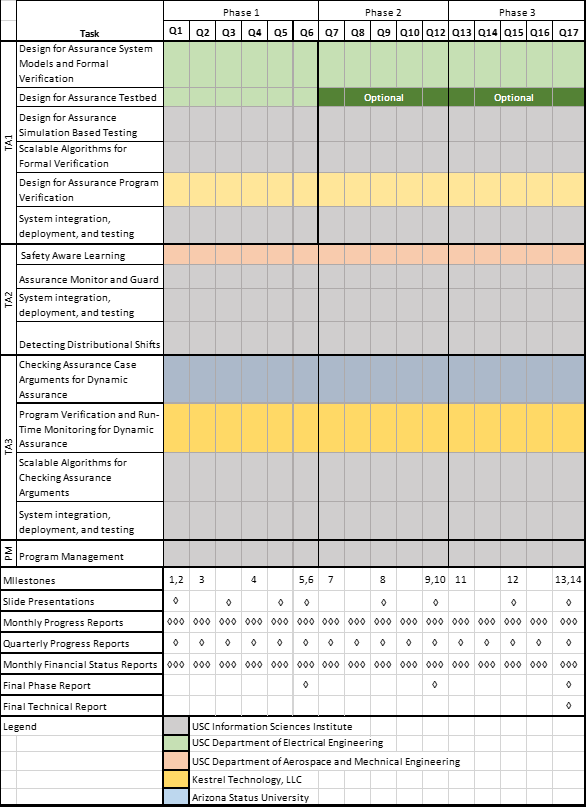
\includegraphics[width=.95\textwidth]{figs/Safeguard_Schedule_V6}
\end{center}
\vspace{-.2in}\caption{Project schedule along with a summary of milestones.  The legend maps task color to organization primary responsible for the task. } 
\label{fig:sandm}
\end{figure}
 

% \section{Level of Effort by Task \textcolor{red}{[Mike/Lisa - 1 pages]}}

% \textcolor{blue}{
% \begin{itemize}
% \item Will be a separate spreadsheet
% \item
% \end{itemize}
% }

\section*{Appendix A: Team Members and Other Information}
\addcontentsline{toc}{section}{Appendix A: Team Members and Other Information}

\baades{This section is mandatory and must include all of the following
components. If a particular subsection is not applicable, state “NONE”.}

\vspace{1ex}

\noindent
\textbf{Team Member Identification}:

\vspace{1ex}

\baades{Provide a list of all team members including the
prime, subcontractor(s), and consultant(s), as applicable. Identify specifically
whether any are a non-US organization or individual, FFRDC and/or Government
entity.}

\begin{centering}

%\small
\begin{tabular}{|p{1.8in}|p{1in}|p{1.1in}|p{0.7in}|p{0.8in}|p{0.7in}|}
\hline
 \textbf{Name} &  \textbf{Role} & \textbf{Organization} & \textbf{Non-US Org?}  & \textbf{Non-US Ind?} &  \textbf{FFRDC or Gov} \\
 \hline
Craig A. Knoblock & Prime & USC & N & N & N\\ \hline
Michael Orosz & Prime & USC & N &  N & N \\ \hline
Satish Thittamaranahalli & Prime & USC & N &  Y & N \\ \hline
Ryan Goodfellow & Prime & USC & N &  N & N \\ \hline
Anoop Kumar & Prime & USC & N & N & N \\ \hline
Satyandra Gupta & Prime & USC & N & N & N \\ \hline
Pierluigi Nuzzo & Prime & USC & N & Y & N \\ \hline
Petros Ioannou & Prime & USC & N & N & N \\ \hline
Chitta Baral & Subcontractor & ASU & N & N & N \\ \hline
Matt Barry & Subcontractor & Kestrel Technology & N & N & N \\ \hline
Douglas Smith & Subcontractor & Kestrel Technology & N & N & N \\ \hline
Henny Sipma & Subcontractor & Kestrel Technology & N & Y & N \\ \hline
\end{tabular} 
\end{centering}

\vspace{1ex}

\noindent
\textbf{Government or FFRDC Team Member Proof of Eligibility to Propose}: NONE

\baades {If
none of the team member organizations (prime or subcontractor) are a
Government entity or FFRDC, state “NONE”.}

\vspace{1ex}

\noindent
\textbf{Government or FFRDC Team Member Statement of Unique Capability}: NONE

\vspace{1ex}

\noindent
\textbf{Organizational Conflict of Interest Affirmations and Disclosure}: NONE

\vspace{1ex}

\noindent
\textbf{Intellectual Property (IP)}: 
\baades {
If no IP restrictions are intended, state “NONE”.
The Government will assume unlimited rights to all IP not explicitly identified as
having less than unlimited rights in the proposal.
For all technical data or computer software that will be furnished to the
Government with other than unlimited rights, provide (per Section VI.B.1) a list
describing all proprietary claims to results, prototypes, deliverables or systems
supporting and/or necessary for the use of the research, results, prototypes
and/or deliverables. Provide documentation proving ownership or possession of
appropriate licensing rights to all patented inventions (or inventions for which a
patent application has been filed) to be used for the proposed project.
}
\begin{centering}

%\small
\begin{tabular}{|p{2.1in}|p{1.2in}|p{1.4in}|p{2in}|}
\hline
\multicolumn{4}{|c|}{COMMERCIAL ITEMS }\\ \hline 
 \textbf{Technical Data, Computer Software To be Furnished With Restrictions} &  \textbf{Basis for Assertion} & \textbf{Asserted Rights Category} & \textbf{Name of Person Asserting Restrictions}  \\  \hline
KT Advance & Developed with mixed funding. & Restricted & David Kulich, Contracts Manager, Kestrel technology, LLC.\\ \hline
\end{tabular} 
\end{centering}

\vspace{1ex}

\noindent
\textbf{Human Subjects Research (HSR)}: NONE

\vspace{1ex}

\noindent
\textbf{Animal Use}: NONE

\vspace{1ex}

\noindent
\textbf{Representations Regarding Unpaid Delinquent Tax Liability or a Felony
Conviction under Any Federal Law}: 
%NONE

\begin{enumerate}
\item
The proposer is  not a corporation that has any unpaid Federal tax liability that has been assessed, for which all judicial and administrative remedies have been exhausted or have lapsed, and that is not being paid in a timely manner pursuant to an agreement with the authority responsible for collecting the tax liability,
\item
The proposer is not a corporation that was convicted of a felony criminal violation under a Federal law within the preceding 24 months.
\end{enumerate}

\vspace{1ex}

\noindent
\textbf{Cost Accounting Standards (CAS) Notices and Certification}:
\baades{
For any proposer who submits a proposal which, if accepted, will result in a CAS-compliant
contract, must include a Disclosure Statement as required by 48 CFR
9903.202. The disclosure forms may be found at
http://www.whitehouse.gov/omb/procurement\_casb
If this section is not applicable, state “NONE”. For further information regarding
this subject, please see www.darpa.mil/work-with-us/additional-baa.
}
NONE


%\section{Appendix B \textcolor{red}{[No Page Count]}}

\section{References}
\bibliographystyle{acm} 
\bibliography{TA3/ta3,TA2/ta2,TA1/ta1}
\end{document}
\clearpage
\newpage


\section{Management Plan}


The Principal Investigator for this effort is Dr. Craig Knoblock who is responsible for all aspects of the effort, will coordinate the parallel team efforts, and will ensure high levels of performance from individual team members.  The Co-P/I, Dr. Michael Orosz, will provide project management and will assist all performers in the execution of the project.    The project team is divided into three working groups (Figure~\ref{fig:org_chart}) corresponding to Technical Areas 1-3, however, members of each team contribute across all project activities.   Table~\ref{fig:Table_Mgmt} defines the major contributions of each project team member to the project tasks.

\begin{figure}[tbhp]
%\vspace{-25pt}
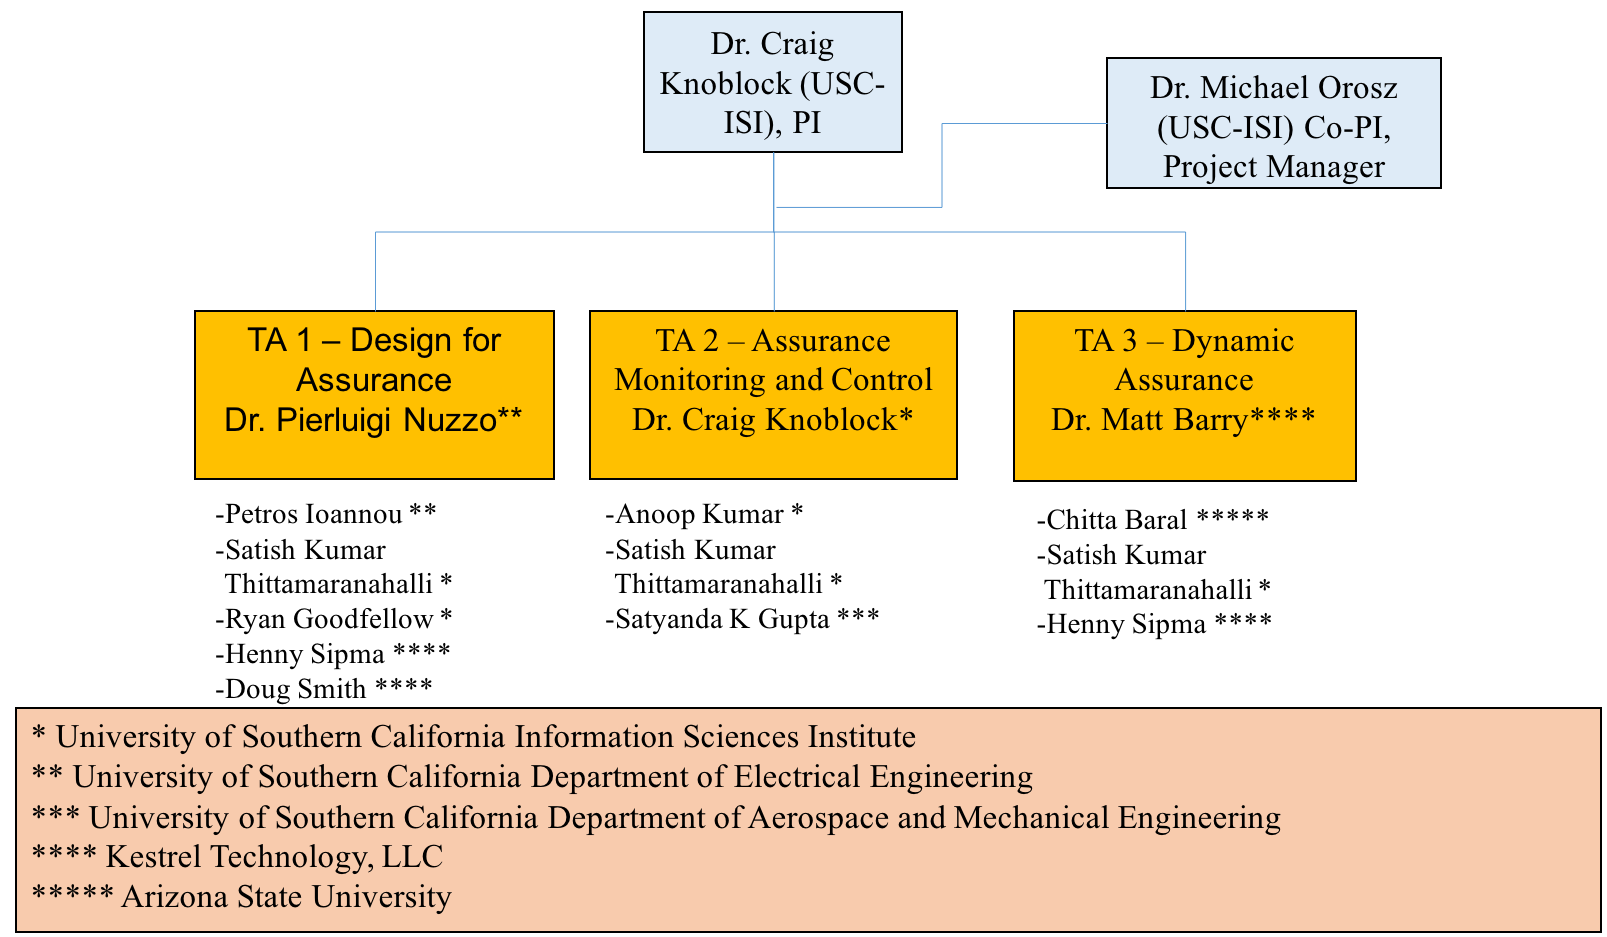
\includegraphics[width=6.0in]{./org-chart2.png}
\caption{\small Organization Chart}
\label{fig:org_chart}
\end{figure}

Coordination: To maximize collaboration and reduce risk to project failure from lack of communication and technical exchange, we plan to employ a wide variety of working styles and communication/coordination so that all can contribute.  At the core of our project will be regularly scheduled meetings bridging the diversely distributed team (Table~\ref{fig:Collaboration_Table}).  These meetings will address project status, identify challenges, implement risk mitigation strategies and participate in technology exchanges and system integration efforts (when appropriate)

\begin{table}[ht]
\caption{\small Project Meetings and Events}
  \centering
  {\footnotesize
\begin{tabular}{|m{3.15in}|m{3in}|} 
\hline
\textbf{Meeting} & \textbf{Frequency} 
\\\hline
Conference calls among investigators (discuss project status, address concerns and project risks) & Weekly
\\
\hline
Technical exchange and coordination meetings using Bluejeans or another videoconference technology & At least twice a month and more frequently as needed
  \\ 
\hline
Face-to-Face meetings (prior to P/I and demonstration meetings) & Every 3 to 6 months and more frequently (especially at the beginning of the project) as needed
 \\\cline{1-2}

\hline
\end{tabular}
}
\label{fig:Collaboration_Table}
\end{table}

\begin{table}[tbhp]
\caption{\small Key Project Team Member Responsibilities}
  \centering
  {\footnotesize
\begin{tabular}{| m{.75in} | m{3.9in}| m{1.5in}|} 
\hline
\textbf{Key Member} & \textbf{Responsibilities} & \textbf{Tasks} 
\\\hline
Dr.\ Craig Knoblock  & Principal Investigator responsible for project, leads TA 2 – Assurance Monitoring and Control.  Will lead the overall project and lead the TA2 team.  Served as the PI on many DARPA projects and has sucessfully led many large teams.    Effort on project:  25\% &
1.1.6, 1.2.2 1.2.3, 1.2.4, 1.3.4, 1.4.1, 
2.1.6, 2.2.2 2.2.3, 2.2.4, 2.3.4, 2.4.1, 
3.1.6, 3.2.2, 3.2.3, 3.2.4, 3.3.4, 3.4.1
\\
\hline
Dr.\ Michael Orosz & Co-Principal Investigator responsible managing the day-to-day operations of the project, assist technical teams as needed, coordinate with TA4 teams.    Has led many large complex multi-disciplined/multi-organizational projects in academic and industry environments.  Effort on project: 50\%
& 1.1.6, 2.1.6, 3.1.6, 1.4.1, 2.4.1, 3.4.1
  \\ 
\hline
Dr.\ Pierluigi Nuzzo 
& 
Co-Principal Investigator.  Leads the TA 1 - Design for Assurance team and conducts research on the formal methods for the design of the TA1 system.  Research experience on methodologies and tools for the design of cyber-physical systems; contracts, interfaces, and compositional methods for embedded system design; the application of automated formal methods and optimization theory to problems in embedded and cyber-physical systems.  Effort on project: 2 months/year (16.6\%)
& 
1.1.1, 2.1.1, 3.1.1 \\
\hline
Dr.\ Matthew Barry
& 
Key personnel.  Leads the TA 3 – Dynamic Assurance.   He will conduct the research on the dynamic assurance case language editors and parsers, the run-time system, and system integrations. Effort on project:  66\%
& 
1.3.2, 2.3.2, 3.3.2\\
\hline
Dr.\ Chitta Baral
& 
Key personnel responsible for learning assurance rules, supporting assurance rules with uncertainty and improving solver speed.  Expertise on ASP solvers, which will be used to reason about the assurance cases. Effort on project: 20\%
& 
1.3.1, 2.3.1, 3.3.1 \\
\hline
Dr.\ Doug Smith 
& 
Key personnel will support formal methods aspects of TA1, and lead the effort on abstract refinement. Expertise in field of automated correct-by-construction program generation.    Effort on project: 40\%
& 
1.1.5, 2.1.5, 3.1.5 \\
\hline
Dr.\ Henny Sipma
& 
Key personnel who will support the program verification tasks under TA1.  Will lead the effort on program verification.   Effort on project:  45\%
& 
1.1.5, 2.1.5, 3.1.5, 1.3.2, 2.3.2, 3.3.2 \\
\hline
Dr.\ Petros Ioannou
& 
Key personnel responsible providing and extending the assurance test bed, which will be available at the start of the project for autonomous vehicles.   Effort on project: 1 month/year (8.3\%)
& 
1.1.2, 2.1.2 (optional), 3.1.2 (optional)
\\
\hline
Dr.\ Satyandra Kumar Gupta
& 
Key Personnel providing autonomous command and control expertise to the TA-2 team.   Will lead the research on safety aware learning on TA2.   Past research on physics-aware decision making to facilitate automation.  Effort on project: 1 month/year (8.3\%)
& 
1.2.1, 2.2.1, 3.2.1 \\
\hline
Dr.\ Anoop Kumar 
& 
Key personnel providing support to the TA 2 project team.  Will lead the research on monitoring \& control and detecting distribution shifts.  Effort on project: 50\%
& 
1.2.1, 1.2.2, 1.2.3, 1.2.4, 2.2.1, 2.2.2, 2.2.3, 2.2.4, 3.2.1, 3.2.2, 3.2.3, 3.2.4\\
\hline
Dr.\ Satish Thittamaranahalli
& 
Key personnel developing scalable algorithms for TA1, TA2, and TA3 project teams.  Has extensive experience on scalable algorithm design, machine learning, and constraint reasoning.  Effort on project: 50\%
& 
1.2.1, 1.2.2, 1.2.3, 1.2.4, 2.2.1, 2.2.2, 2.2.3, 2.2.4, 3.2.1, 3.2.2, 3.2.3, 3.2.4, 1.1.4, 2.1.4, 3.1.4 \\
\hline
Dr.\ Ryan Goodfellow
& 
Key personnel providing support to the TA-1 project. Will lead the research on simulation-based testing.  Has extensive experience on simulation-based testing.  Effort on project:  30\%
& 
1.1.3, 2.1.3, 3.1.3 \\

\cline{1-2}

\hline
\end{tabular}
}
\label{fig:Table_Mgmt}
\end{table}



\newpage
\section{Personnel, Qualifications and Commitment}

{\bf Dr.\ Craig Knoblock}, the PI on this effort, is a Research Professor of both Computer Science and Spatial Sciences at the University of Southern California (USC) and Director of the Intelligent Systems Division at the USC Information Sciences Institute.   He received his Ph.D. from Carnegie Mellon University in computer science. 
%His research focuses on techniques for describing, acquiring, and exploiting the semantics of data.  
In previous projects he has worked on developing  scalable approaches to execution monitoring, accurate detection of sensor failures, and   automatic modeling and reconstruction of sensors.  He has published more than 300 journal articles, book chapters, and conference papers on these topics.  Dr. Knoblock is a Fellow of the Association for the Advancement of Artificial Intelligence (AAAI), a Distinguished Scientist of the Association of Computing Machinery (ACM), a Senior Member of IEEE, past President and Trustee of the International Joint Conference on Artificial Intelligence.
%and winner of the 2014 Robert S. Engelmore Award.  

{\bf Dr.\ Michael Orosz}, a Co-PI on this effort, is a Research Associate Professor of Civil and Environmental Engineering at the University of Southern California (USC) and Research Director of the Decision Systems Group at the USC Information Sciences Institute.  Dr. Orosz has over 30 years’ experience in commercial and government software development, basic and applied research, project management, academic research and has developed and deployed several commercially successful products.  His research interests are in machine learning and decision analytics as applied to intelligence analysis and autonomous command and control such as smart building controls.    Dr. Orosz has extensive experience in managing large complex multi-disciplined/multi-teamed research projects. %funded by DARPA, DHS, DoD, DoE, Industry, NASA, NRO, NSA and ONR.   
He received his Ph.D. in computer science from the University of California, Los Angeles.

{\bf Dr.\ Pierluigi Nuzzo}, a Co-PI on this project, is an Assistant Professor in the Department of Electrical Engineering at the University of Southern California. He received the Ph.D. in Electrical Engineering and Computer Sciences from the University of California at Berkeley. 
%in 2015, and the Laurea degree (MS) in electrical engineering (summa cum laude) from the University of Pisa, Italy, and the Sant'Anna School of Advanced Studies, Pisa, Italy.
%
%He has four years of research experience in analog and mixed signal circuit design as a researcher at IMEC, Leuven, Belgium, and over 10 years experience in design methodologies and tools for mixed-signal integrated circuits and cyber-physical systems, as a researcher at the University of Pisa, IMEC, UC Berkeley, and USC. 
His research interests
include: methodologies and tools for cyber-physical system and mixed-signal
system design; contracts, interfaces and compositional methods for embedded
system design; the application of formal methods and optimization theory to problems in embedded and cyber-physical systems and electronic design automation. 
%
Prof. Nuzzo received %First Place in the operational category and Best Overall
%Submission in the 2006 DAC/ISSCC Design Competition, 
a Marie Curie Fellowship
from the European Union in 2006, 
the University of California at Berkeley EECS
departmental fellowship in 2008, 
%the University of California at Berkeley Outstanding Graduate Student Instructor Award in 2013, 
the IBM Ph.D.
Fellowship in 2012 and 2014, 
%the Best Paper Award from the International Conference on Cyber-Physical Systems (ICCPS) in 2016, 
and the David J.~Sakrison Memorial Prize in 2016 for his doctoral research. 
%He is an author of 1 patent and over 60 publications.

{\bf Dr.\ Satyandra K. Gupta} is Smith International Professor in the Department of Aerospace and Mechanical Engineering at the University of Southern California. %Prior to joining the University of Southern California, he was a Professor in the Department of Mechanical Engineering and the Institute for Systems Research at the University of Maryland. He was the founding director of the Maryland Robotics Center and the Advanced Manufacturing Laboratory at the University of Maryland. 
He served as a program director for the National Robotics Initiative at the National Science Foundation from September 2012 to September 2014.  Dr. Gupta's interest is in the area of physics-aware decision making to facilitate automation. He has published more than 300 technical articles. He is a fellow of the American Society of Mechanical Engineers (ASME) and editor of ASME Journal of Computing and Information Science in Engineering. Dr. Gupta has received the Young Investigator Award from the Office of Naval Research in 2000, CAREER Award from the National Science Foundation in 2001, Presidential Early Career Award for Scientists and Engineers (PECASE) in 2001, Invention of the Year Award at the University of Maryland in 2007, Kos Ishii-Toshiba Award from ASME in 2011, and Excellence in Research Award from ASME in 2013.%, and Distinguished Alumnus Award from Indian Institute of Technology, Roorkee in 2014. %He has also received seven best paper awards at conferences.

{\bf Ryan Goodfellow} is a computer scientist at ISI working in combined cyber physical simulation and emulation platform development. His formal background is in simulation algorithms and modeling techniques using differential-algebraic equations (DAE). He has applied this knowledge in the CPS space by integrating DAE modeling languages and simulation engines with network testbeds to create comprehensive scientific experimentation platforms for cyber-physical systems. These experimentation platforms have been used in the power grid research space. %Ryan is a lead developer on the Deter network testbed, with a strong background in networked and distributed systems engineering. %He is also a combat veteran, serving as a non-commissioned officer and SIGINT team lead for a multi-functional intelligence team in Afghanistan.

{\bf Dr.\ Petros Ioannou} is a Professor in the Department of Electrical Engineering, Director of the Center for Advanced Transportation Technologies and Associate Director for Research for the DOT supported University Transportation Center at USC. He received his MS and PhD from the University of Illinois at Urbana Champaign in Mechanical and Electrical Engineering, respectively. His research interests are in robust adaptive control, vehicle dynamics and control, human factors and safety, automated vehicles, nonlinear systems and Intelligent transportation Systems.  He received the 2016 IEEE Transportation Technologies field award and the 2016 IEEE Control system society Transition to Practice Award. He is a Fellow of IEEE, IFAC and IET and author/coauthor of 8 books and over 400 papers.

{\bf Dr.\ Matthew Barry} will serve as lead for the TA3 tasks. %He will implement the dynamic assurance case language editors and parsers, the run-time system, and system integrations.  He will implement the assurance case arguments and the API for updating argument structure and content.  
Dr. Barry currently is CEO at Kestrel Technology LLC, and previously spent 20 years in NASA space mission operations at the Jet Propulsion Lab and Johnson Space Center.  At NASA Headquarters he led the introduction of dependability case requirements and plans for flight computing systems in upcoming manned space exploration missions, as well as the development of Agency-level software-related safety-critical control system requirements.  He recently served as a Principal Investigator on DHS/Cyber S\&T STAMP (Static Tool Analysis Modernization Program), DARPA CSFV (Crowd Sourced Formal Verification), three NASA Aeronautics R\&D projects, and the AFRL-sponsored Static Analysis of Numerical Algorithms project.  Dr. Barry earned BSME, MS, and PhD degrees in mechanical engineering, and an MBA degree, from Rice University.  

{\bf Dr.\ Henny Sipma} will support the program verification tasks under TA1.  %She is the key person behind the company's {\em KT Advance\/} and {\em KT Transferal\/} static analysis products, and the designer and programmer of the company's core {\em CodeHawk\/} abstract interpretation engine. 
Dr. Sipma currently is the CTO at Kestrel Technology LLC.  She has spent the past 10 years with Kestrel Technology as a static analysis expert; previously developed and taught static analysis techniques as senior research associate at Stanford University for eight years; and developed industrial process controls as an senior systems analyst at Shell.  She has been Principal Investigator or company lead on several recent R\&D projects for Federal agencies, including two projects under the IARPA STONESOUP (Securely Taking On New Executable Software of Uncertain Provenance) program; the DHS Cyber S\&T Gold Standard project; and the DARPA-sponsored STAC (Space-Time Analysis for Cybersecurity) and MUSE (Mining and Understanding Software Enclaves) programs.  Dr. Sipma earned 
%a BS degree in chemistry and an MS degree in chemical engineering at the University of Groningen in The Netherlands, and 
MS and PhD degrees in computer science from Stanford University.  

{\bf Dr.\ Douglas R.\ Smith} will support formal methods aspects of TA1, including the enforcement of safety properties and the generation of monitors.  He is President of Kestrel Technology LLC and Principal Scientist at Kestrel Institute.  He is a Fellow of the American Association of Artificial Intelligence (AAAI) and an ASE Fellow (Automated Software Engineering).  From 1986 to 2000, he taught an advanced graduate course on correct-by-construction software development at Stanford.  
%Dr. Smith has led the development of a series of software synthesis systems, including KIDS (Kestrel Interactive Development System), Specware, Designware, and Planware. 
%Applications domains have included a variety of complex high-performance planners and schedulers for the US Air Force.  He leads current projects on the generation of air mission plans and cyberoperations.  
Other recent projects focused on automated policy enforcement \cite{SmithD0703,SmithD08}, synthesis of secure network protocol codes, and the synthesis of high-performance constraint-solvers\cite{SmithD08c,SmithD13}.  Dr. Smith has over 30 years experience in the field of automated correct-by-construction program generation and has published over 100 papers. He has one patent.  He received the Ph.D. in Computer Science from Duke University% in 1979.  

{\bf Dr. Chitta Baral} is a Professor in the Department of Computer Science and Engineering at Arizona State University. He will support the TA3 efforts on Learning assurance rules, supporting assurance rules with uncertainty and improving solver speed. Dr. Baral has expertise in various aspects of autonomy and Artificial Intelligence. 
He wrote the first book on answer set programming (published by Cambridge University Press) the formal language behind our assurance rules. Some of his other works relevant to this proposal are: goal specification for autonomous systems, automatic construction of control rules for autonomous systems that satisfy given goals, combining machine learning with reasoning in various contexts, including image understanding. %He is the President of KR Inc. He is an associate editor of AIJ and has been an associate editor of JAIR.

{\bf Dr.\ Satish Kumar Thittamaranahalli (T. K. Satish Kumar)} leads the Collaboratory for Algorithmic Techniques and Artificial Intelligence (CATAI) at USC's Information Sciences Institute. He has published over 60 papers on numerous topics in Artificial Intelligence spanning such diverse areas as Constraint Reasoning, Planning and Scheduling, Probabilistic Reasoning, Robotics, Combinatorial Optimization, Approximation and Randomization, Heuristic Search, Model-Based Reasoning, Knowledge Representation and Spatio-Temporal Reasoning. %He %has served on the Program Committees of many international conferences in Artificial Intelligence
He and is a winner of the 2016 Best Robotics Paper Award and the 2005 Best Student Paper Award from the International Conference on Automated Planning and Scheduling. 
Dr. Kumar received his PhD in Computer Science from Stanford University. %In the past, he has also been a Visiting Student at the NASA Ames Research Center, a Postdoctoral Research Scholar at the University of California, Berkeley, a Research Scientist at the Institute for Human and Machine Cognition, a Visiting Assistant Professor at the University of West Florida, and a Senior Research and Development Scientist at Mission Critical Technologies.

\textbf{Dr.\ Anoop Kumar} is a senior computer scientist at USC ISI and has broad expertise in machine learning, statistical modeling, and software engineering.  Dr.\ Kumar is the technical lead on the DARPA RSPACE program and has played a vital role in developing a system that fuses air operations data from multiple sources, maintains world state, and issues warnings. Previously, he led the research and development of the BBN’s election forecasting system for the IARPA OSI program. %Dr.\ Kumar played a significant role in the DARPA DEFT program by developing a model to support integration of output from multiple NLP algorithms. He has contributed at the development to management levels on government research contracts and commercial projects. 
Dr.\ Kumar helped design and develop BBN's commercially available, hosted speech and medical transcription services offering. 

\begin{table}[!tbh]
\begin{footnotesize}
\vspace{-0.1in}

\begin{tabular}{lll}
\begin{tabular}[t]{|l|@{}c@{}|@{}c@{}|@{}c@{}|@{}c@{}|} \hline
Project & Status & \multicolumn{3}{ c| }{Hours} \\ \cline{3-5}
& & P1 & P2 & P3 \\ \hline



\multicolumn{5}{ |c| }{ \textbf{Craig Knoblock} } \\ \cline{1-5}
Safeguard & Pro & 770 & 641 & 641 \\ \cline{1-5}
ELICIT & Cur & 308 & 256 & 120 \\ \cline{1-5}
WTNIC & Cur & 11 & 0 & 0 \\ \cline{1-5}
EFFECT & Cur & 641 & 107 & 0 \\ \cline{1-5}
LinkedMaps & Cur & 203 & 25 & 0 \\ \cline{1-5}
PRINCESS & Cur & 608 & 96 & 0 \\ \cline{1-5}
SCHARP & Cur & 481 & 54 & 0 \\ \cline{1-5}
MINT & Pen & 650 & 534 & 285 \\ \cline{1-5}

\multicolumn{5}{ |c| }{ \textbf{Michael Orosz} } \\ \cline{1-5}
Safeguard & Pro & 1560 & 1300 & 1300  \\ \cline{1-5}
SMC/SY & Cur & 1803 & 0 & 0  \\ \cline{1-5}

\multicolumn{5}{ |c| }{ \textbf{Matthew Barry} } \\ \cline{1-5}
Safeguard & Pro & 2078 & 1690 & 1554 \\ \cline{1-5}
Starlite & Cur & 1840 & 1692 & 0 \\ \cline{1-5}



\multicolumn{5}{ |c| }{ \textbf{Anoop Kumar} } \\ \cline{1-5}
Safeguard & Pro & 1560 & 1300 & 1300 \\ \cline{1-5}

\end{tabular}
&
\begin{tabular}[t]{|l|@{}c@{}|@{}c@{}|@{}c@{}|@{}c@{}|} \hline
Project & Status & \multicolumn{3}{ c| }{Hours} \\ \cline{3-5}
& & P1 & P2 & P3 \\ \hline

\multicolumn{5}{ |c| }{ \textbf{Pierluigi Nuzzo} } \\ \cline{1-5}
Safeguard & Pro & 520 & 433 & 433  \\ \cline{1-5}
Mirage & Cur & 433 & 0 & 0  \\ \cline{1-5}

\multicolumn{5}{ |c| }{ \textbf{Satyandra Gupta} } \\ \cline{1-5}
Safeguard & Pro & 260 & 217 & 217 \\ \cline{1-5}
Human   & Cur & 22 & 0 & 0 \\ \cline{1-5}
Vehicles & Cur & 36 & 0 & 0 \\ \cline{1-5}
Robot & Cur & 116 & 0 & 0 \\ \cline{1-5}
Assembly & Cur & 33 & 0 & 0 \\ \cline{1-5}
Solar & Cur & 4 & 0 & 0 \\ \cline{1-5}

\multicolumn{5}{ |c| }{ \textbf{Petros Ioannou} } \\ \cline{1-5}
Safeguard & Pro & 260 & 217 & 217 \\ \cline{1-5}
CPS & Cur & 130 & 0 & 0 \\ \cline{1-5}

\multicolumn{5}{ |c| }{ \textbf{Ryan Goodfellow} } \\ \cline{1-5}
Safeguard & Pro & 936 & 780 & 780 \\ \cline{1-5}
STEAM & Cur & 416 & 0 & 0 \\ \cline{1-5}


\end{tabular}
&
\begin{tabular}[t]{|l|@{}c@{}|@{}c@{}|@{}c@{}|@{}c@{}|} \hline
Project & Status & \multicolumn{3}{ c| }{Hours} \\ \cline{3-5}
& & P1 & P2 & P3 \\ \hline

\multicolumn{5}{ |c| }{ \textbf{Chitta Baral} } \\ \cline{1-5}
Safeguard & Pro & 659 & 485 & 485 \\ \cline{1-5}
PostdocBP & Cur & 176 & 0 & 0 \\ \cline{1-5}
Languages & Pen & 528 & 264 & 264 \\ \cline{1-5}
CAREER & Pen & 88 & 44 & 44 \\ \cline{1-5}
CHS & Pen & 510 & 255 & 0 \\ \cline{1-5}

\multicolumn{5}{ |c| }{ \textbf{Doug Smith} } \\ \cline{1-5}
Safeguard & Pro & 1222 & 984 & 840 \\ \cline{1-5}
RSPACE & Cur & 342 & 0 & 0 \\ 
\cline{1-5}
PLANX & Cur & 154 & 0 & 0 \\ 
\cline{1-5}
HACCS & Pen & 923 & 769 & 769 \\ 
\cline{1-5}

\multicolumn{5}{ |c| }{ \textbf{Henny Sipma} } \\ \cline{1-5}
Safeguard & Pro & 1372 & 962 & 840 \\ \cline{1-5}
STAC & Cur & 797 & 0 & 0 \\ \cline{1-5}

\multicolumn{5}{ |c| }{ \textbf{Satish Thittamaranahalli} } \\ \cline{1-5}
Safeguard & Pro & 1560 & 1300 & 1300 \\ \cline{1-5}
MapF & Cur & 103 & 103 & 0 \\ \cline{1-5}

\end{tabular}
\end{tabular}

\end{footnotesize}
\caption{Individual commitments of key personnel}
\label{tab:Commitments}
\vspace{-0.2in}
\end{table}

\clearpage
\newpage
\section{Capabilities}


%\subsection{University of Southern California}
USC has strengths in number of areas that are closely related to the proposed work:
\begin{itemize}[itemsep=0pt,leftmargin=*]
\item Dr.\ Nuzzo 
%has over 10-year research experience in embedded system design, from mixed-signal chip design (analog-to-digital converters, frequency synthesizers, software-defined radio), to methodologies and tools for mixed-signal integrated circuits and Cyber-Physical Systems (CPSs), and the application of formal methods and optimization theory to problems in embedded and cyber-physical systems and electronic design automation.  
%His doctoral work 
has done extensive research on contracts and compositional methods for heterogeneous system design and design space exploration, with application to aircraft electric power systems and environmental control systems. His work has helped transition rigorous system design foundations, innovative design methodologies, and new systems engineering paradigms to industry (IBM, United Technologies). 
\item Dr.\ Satyandra K. Gupta has worked on autonomous surface vehicles, autonomous ground vehicles for operation on rugged terrains, and autonomous flapping wing aerial vehicles.   His group has developed a hierarchal decision making approach for realizing autonomous systems. 
%This approach combines task planning and assignment, deliberative trajectory planning, reactive collision avoidance behaviors, and trajectory tracking control layers. 
His group has also developed new methods for learning reactive behaviors in adversarial environments and COLREGS compliant trajectory planning. \item Dr.\ Knoblock has developed methods that learn the relationships between sensors to both identify failures and changes in sensor and reconstruct those sensors, providing estimates of the accuracy of the reconstructed sensors.  
\item Ryan Goodfellow has extensive experience in simulation based testing through high-fidelity CPS testbed environment development and operation, using the Deter network testbed as the core which has supported several large scale government projects from a variety of agencies and thousands of users. %we have developed sophisticated CPS experiments under programs such as NFS RIPS, NIST SmartCities and the DHS Cybersecurity showcase.
\item Dr.\ Ioannou %helped  design and implement adaptive cruise control systems in collaboration with Ford Motor Company, which was commercialized four years before any other company. He 
worked on several DOT funded projects on automated vehicles and intelligent highway systems where he demonstrated his vehicle control designs for safety and performance on actual automated vehicles in test trucks and I-15 highway.
\item Drs.\ Knoblock, Kumar, and Thittamaranahalli have developed highly scalable approaches for monitoring message traffic to identify potential problems and issue warnings and alerts. 
\item Dr. Thittamaranahalli has developed state-of-the-art methods for efficiently solving large-scale search and optimization problems. %These techniques will be applicable in TA2 for safety-aware learning and planning, in TA2 for assurance monitoring and control, and in TA3 for dynamic assessment of assurance cases.

\end{itemize}
%\subsection{Kestrel Technology LLC}

Kestrel Technology's strength is in program analysis, specifically static analysis of both source and binary targets.  The company performs applied R\&D and product development for a variety of static analysis applications  pivoting primarily on the abstract interpretation technique.  The company recently initiated development of program analysis applications using logical equivalence techniques. As a provider of verification evidence in the form of mathematical proofs, the company also has expertise in the design and development of assurance case arguments for high-integrity systems using such evidence. %The company is engaged in a partnership with Wind River Systems to develop program analysis tools for its embedded system developers.  Many of Wind River's customers must develop their products under safety and certification standards, including those using safety cases.  

   

%\subsection{Arizona State University}
Chitta Baral at Arizona State University has developed various software to learn assurance rules and various ASP solvers, which he has made available as open-source.

Most of the software carried forward for implementation or derivation is open source.  The single exception is Kestrel Technology's {\it KT Advance\/} static analysis tool (TA1), in particular the abstract interpretation engine therein, which is company proprietary and is US EAR export-controlled.   
%Owing to mixed funding for the development of that technology 
We will continue to provide the Federal government a restricted use license for that particular item.

There are no specialized facilities, data, or GFE required for this effort. 


\section{Statement of Work}
We propose work for TA 1 – TA 3 for all three phases. All tasks span the four years of the program. For each task we provide an objective, the high-level approach (focusing on the responsibilities of each contributing organization), and the specific approach and milestones planned for each task for each phase. On all tasks, we will deliver design documents, software implementations, demonstrations, and publications. With the exception of several tasks accomplished by Kesler Technology, LLC, all tasks that accomplished at a university (USC/ISI, USC, and ASU) are believed to be fundamental research.   
%\usepackage[table]{xcolor}

{\scriptsize

\begin{longtable} {|p{\textwidth} | }

\hline

\textcolor{blue} {\footnotesize {\textbf{Tasks 1.1.1, 2.1.1, 3.1.1 -Design for Assurance System Models and Formal Verification (USC)}}} \\ \hline
Objective:  Develop contract-based formalisms and mapping tools to represent and reason about LE-CPSs at multiple levels of abstraction and generate assurance cases.  Undertake scalable formal verification and synthesis via Satisfiability Modulo Convex Programming. \\ \hline
Approach:  Develop modeling formalisms to represent components and contracts for LE-CPSs, including physical plant (e.g., autonomous vehicle, sensors, actuators, environment, controllers, and learning components. Formalisms will encompass different control and learning architectures (e.g., neural networks, statistical methods, graphical models, ensemble methods, decision trees) and support mapping between abstractions.   Develop a formal domain-specific language to capture and formalize requirements on LE components, systems, and their dynamics as contracts.   Develop a unifying framework and efficient algorithms to reason about the combination of discrete and continuous dynamics and constraints in the presence of uncertainties in LE cyber-physical systems \\ \hline
Phase 1 (1.1.1):  Milestone 1: Develop initial design followed by development and testing of individual components.  Milestone 2:  Library of components and contracts for the autonomous vehicle application driver.  Milestone 4: Library of components and contracts for the platforms provided by TA4 performers. Extension of the methodology and to support up to 20 continuous dimensions and 2 learning components for the 2 application drivers from TA4.  Milestone 6: -Prototype toolkit (software package) for capturing requirements, for translating them into contracts, for analyzing and validating them using contract operations and relations.  Prototype toolkit for capturing probabilistic requirements and behaviors of LE components, systems, and their dynamics, for translating them into stochastic assume-guarantee contracts, for analyzing and validating them using contract operations and relations, and for synthesizing design and verification artifacts from contracts.  Extension of the SMC framework and toolkit to support reactive and robust task and trajectory planning in the presence of uncertainties. \\ \hline
Phase 2 (2.1.1) Milestone 7: Refinement of design.  Milestone 9: extension of methodology, design, toolkits and libraries to support 40 continuous dimensions, 4 LECs, 30\% monitoring overhead. Extension of the SMC framework and toolkit from Phase 1 to support verification and synthesis on system with 40 dimensions and 4 LECs.  Milestone 10: Demonstration of the SMC framework and toolkit.  Contribution to Phase II report and dissemination of the results in conferences and journals. \\ \hline
Phase 3 (3.1.1) Milestone 11: Update design based on Phase II demo.  Milestones 12-13:  extend methodology, design, toolkits and libraries to support 100 dimensions, 6 LECs and 10\% monitoring overhead.   Milestone 14: Undertake Phase III demonstration on both platforms and submit final project report. \\ \hline
\textcolor{blue} {\footnotesize {\textbf{Tasks 1.1.2, 2.1.2, 3.1.2: Design for Assurance Testbed (USC)} }}\\ \hline
Objective:  Develop a simulation test bed for data generation and LE algorithm testing, redesign and/or refinement.   Simulator used as the test bed until the TA4 platforms are available.   Test bed will be used for internal research/prototype after TA4 platform availability. \\ \hline
Approach:  Leverage previous work on microscopic traffic simulations in urban and rural environments using the commercial software VISSIM and Vortex Studio and built in extensions for automated driving.   Develop testbed for autonomous vehicles in road/off-road environments to allow LEs to collect data, learn and make control decisions on line and in real time by simulating scenarios. The testbed together with analytical tools used to refine and redesign LEs and control algorithms by taking into account effects revealed by the simulation and not accounted for in the design stage.    In the event the TA4 platforms are not available, the test bed will be extended further by integrating all the LE components, controllers and sensors for demonstration purposes and evaluation of the proposed methodology. \\ \hline
Phase 1 (1.1.2):  Milestones 1-2:  Extension of existing simulator test beds.  Milestones 3-5:  Testing of individual components under normal and unpredicatble situations and demonstrating the results in VISSIM under several different driving scenarios. \\ \hline
Phase 2 (2.1.2) – Optional:  Milestones 7-8:  Extension of existing simulator test beds to support the TA1-TA3 teams.  Milestones 9-10:  Support demonstration of technology capable of supporting 40 dimensions, 4 LECs and 30\% monitoring overhead. \\ \hline
Phase 3 (3.1.2) – Optional:  Milestones 11-12:  Extension of existing simulator test beds to support the TA1-TA3 teams.  Milestones 13-14:  Support demonstration of technology capable of supporting 100 dimensions, 6 LECs and 10\% monitoring overhead. \\ \hline
\textcolor{blue} {\footnotesize {\textbf{Tasks 1.1.3, 2.1.3, 3.1.3: Design for Assurance Simulation Based Testing (USC/ISI)}}} \\ \hline
Objective:  Develop external Discrete Control Mechanisms for OpenModelica.  Develop/package virtual-machine based static time dilation systems. Undertake network testbed integration and develop physical system behavioral analysis tooling. \\ \hline
Approach:  Leverage previous external discrete control mechanisms for DAEs, implement similar facilities for OpenModelica to allow LEs to observe and control a physical system over a network. Contributions pushed back upstream to OpenModelica project.  Implement DieCast for modern libvirt.  Develop tooling to deploy integrated CPS models on the Deter network testbed. Apply modern DAE control theory in the form Modelica analysis packages usable by non DAE experts. \\ \hline
Phase 1 (1.1.3):  Milestones 1-2:  Initial CPS simulation concept and components.  Milestones 3-5:  Testing of individual components under normal and unpredictable situations and demonstrating the results capable of meeting 20 dimensions, 2 LECs and 50\% or under monitoring overhead conditions.   Milestone 6: Demonstrate technology in Phase I demonstration, contribute to Phase I final report and disseminate software and publications. \\ \hline
Phase 2 (2.1.3):  Milestones 7-8:  Apply lessons learned from Phase I and extend existing simulations to support 30 dimensions, 3 LECs and 40\% monitoring overhead.  Milestones 9-10:  Support demonstration of technology capable of supporting 40 dimensions, 4 LECs and 30\% monitoring overhead.  Contribute to Phase II final report and disseminate software and publications. \\ \hline
Phase 3 (3.1.3):  Milestones 11-12:  Apply lessons learned from Phase II and extend existing simulations to support 70 dimensions, 5 LECs and 20\% monitoring overhead.  Milestones 13-14:  Support demonstration of technology capable of supporting 100 dimensions, 6 LECs and 10\% monitoring overhead.  Contribute to Phase III final report and disseminate software and publications. \\ \hline
\textcolor{blue} {\footnotesize {\textbf{Tasks 1.1.4, 2.1.4, 3.1.4: Scalable Algorithms for Formal Verification (USC/ISI)}}} \\ \hline
Objective: Develop innovative algorithms for scalable formal verification. \\ \hline
Approach: Use state-of-the-art techniques for solving combinatorial problems with discrete/continuous variables and hybrid constraints. \\ \hline
Phase 1 (Task 1.1.4): Milestones 1-2: Develop initial design plan and initial concepts. Milestones 3-5: Integrate framework that is capable of supporting 20 dimensions, 2 LECs and 0.1x trials to assurance. Milestone 6: Participate in Phase I demonstration, contribute to Phase I final report and disseminate software and publications. \\ \hline
Phase 2 (Task 2.1.4): Milestones 7-8: Apply lessons learned from Phase I and extend existing design to support 30 dimensions, 3 LECs and 0.05x trials to assurance. Milestones 9-10: Demonstrate technology capable of supporting 40 dimensions, 4 LECs and 0.01x trials to assurance. Participate in Phase II demonstration, contribute to Phase II final report and disseminate software and publications. \\ \hline
Phase 3 (Task 3.1.4): Milestones 11-12: Apply lessons learned from Phase II and extend design/approach to support 70 dimensions, 5 LECs and 0.005x trials to assurance. Milestones 13-14: Demonstrate technology capable of supporting 100 dimensions, 6 LECs and 0.001x trials to assurance. Complete integration of technology into TA4 platform. Contribute to Phase III final report and disseminate software and publications. \\ \hline
\textcolor{blue} {\footnotesize {\textbf{Tasks 1.1.5, 2.1.5, 3.1.5: Design for Assurance Program Verification (Kestrel Technology, LLC)}}} \\ \hline
Objective: Develop and integrate program analysis and monitor synthesis functionality with TA1 functions and services and integrate combined TA1 functions with TA4 platform. \\ \hline
Approach: Integrate existing analysis tools into development environment.  Design and implement abstract domains and properties for one or more modeling layers.  Design and implement analyzer front-end for modeling layers.  Implement test framework for verification tools.  Implement content providers and/or consumers for DAC via DAC API.  Leverage existing algorithms and tools to generate monitors for assumptions and unproven safety constraints. Integrate program analysis and monitor synthesis functionality with TA1 functions and services, integrate combined TA1 functions with TA4 platform.   Prepare software and data installation kits and operating instructions;install software and confirm configuration. \\ \hline
Phase 1 (1.1.5) : Milestones 1-2:  Initial framework design and unit tools, TA1-TA3 interfaces defined. Milestones 3-5:  Testing of individual components/tools capable of meeting 20 dimensions, 2 LECs and 50\% or under monitoring overhead conditions.   Milestone 6: Demonstrate technology in Phase I demonstration, contribute to Phase I final report and disseminate software and publications. \\ \hline
Phase 2 (2.1.5): Milestones 7-8:  Apply lessons learned from Phase I and extend existing design to support 30 dimensions, 3 LECs and 40\% monitoring overhead.  Milestones 9-10:  Support demonstration of technology capable of supporting 40 dimensions, 4 LECs and 30\% monitoring overhead.  Contribute to Phase II final report and disseminate software and publications. \\ \hline
Phase 3 (3.1.5): Milestones 11-12:  Apply lessons learned from Phase II and extend existing simulations to support 70 dimensions, 5 LECs and 20\% monitoring overhead.  Milestones 13-14:  Support demonstration of technology capable of supporting 100 dimensions, 6 LECs and 10\% monitoring overhead.  Contribute to Phase III final report and disseminate software and publications. \\ \hline
\textcolor{blue} {\footnotesize {\textbf{Tasks 1.1.6, 2.1.6, 3.1.6: System integration, deployment, and testing (USC/ISI)}}} \\ \hline
Objective: Develop and implement integration, testing and deployment plan supporting TA1 for all three phases. \\ \hline
Approach: Develop an internal TA1 integration and testing plan (unit tests, etc.) and, in close collaboration with TA2 and TA3 performers on project, develop an overall TA1-TA3 integration and testing plan.  Working with TA4 performers, extend and execute plan for TA4 platform (when available). \\ \hline
Phase 1 (1.1.6): Milestones 1-2:  Develop initial integration and testing plan and implement on unit testing.  Milestones 3-5:  Oversee integration and testing of TA1-TA3 components for system capable of supporting 20 dimensions, 2 LECs and 50\% or less monitoring overhead.   Milestone 6: Complete integration of technology into TA4 testbeds, contribute to Phase I final report and disseminate software and publications. \\ \hline
Phase 2 (2.1.6): Milestones 7-8:  Apply lessons learned from Phase I and extend existing integration and testing plan to support 30 dimensions, 3 LECs and 40\% monitoring overhead.  Milestones 9-10:  Support demonstration of technology capable of supporting 40 dimensions, 4 LECs and 30\% monitoring overhead.  Complete integration of technology into TA4 platforms.  Contribute to Phase II final report and disseminate software and publications. \\ \hline
Phase 3 (3.1.6): Milestones 11-12:  Apply lessons learned from Phase II and extend existing integration and testing plan to support 70 dimensions, 5 LECs and 20\% monitoring overhead.  Milestones 13-14:  Support demonstration of technology capable of supporting 100 dimensions, 6 LECs and 10\% monitoring overhead.  Complete integration of technology into TA4 platform.  Contribute to Phase III final report and disseminate software and publications. \\ \hline
\textcolor{blue} {\footnotesize {\textbf{Tasks 1.2.1, 2.2.1, 3.2.1: Safety Aware Learning (USC)} }}\\ \hline
Objective: Enable the system to learn efficiently without violating safety constraints. \\ \hline
Approach: Integrate LECs with search methods to select the optimal actions/maneuvers to maximize mission utility. \\ \hline
Phase 1 (Task 1.2.1): Milestones 1-2:  Develop initial design plan and initial concepts. Milestones 3-5:  Integrate two LECs with search methods and integrate into framework that is capable of supporting 20 dimensions, 2 LECs and 50\% or less monitoring overhead.   Milestone 6: Participate in Phase I demonstration, contribute to Phase I final report and disseminate software and publications. \\ \hline
Phase 2 (Task 2.2.1): Milestones 7-8:  Apply lessons learned from Phase I and extend existing design to support 30 dimensions, 3 LECs and 40\% monitoring overhead.  Milestones 9-10:  Support demonstration of technology capable of supporting 40 dimensions, 4 LECs and 30\% monitoring overhead.  Participate in Phase II demonstration.  Contribute to Phase II final report and disseminate software and publications. \\ \hline
Phase 3 (Task 3.2.1): Milestones 11-12:  Apply lessons learned from Phase II and extend design/approach to support 70 dimensions, 5 LECs and 20\% monitoring overhead.  Milestones 13-14:  Support demonstration of technology capable of supporting 100 dimensions, 6 LECs and 10\% monitoring overhead. Complete integration of technology into TA4 platform.  Contribute to Phase III final report and disseminate software and publications. \\ \hline
\textcolor{blue} {\footnotesize {\textbf{Tasks 1.2.2, 2.2.2, 3.2.2: Assurance Monitor and Guards (USC)}}} \\ \hline
Objective: Build scalable algorithms for assurance monitoring of architectural and safety constraints \\ \hline
Approach: Use physical models to reduce processing of sensor information for assurance monitoring. Use Variable Elimination to handle uncontrollable, Adversarially controlled, or unobservable variables \\ \hline
Phase 1 (Task 1.2.2): Milestones 1-2:  Develop initial design plan and initial concepts.  Milestones 3-5:  Develop monitors for two LECs and integrate into framework that is capable of supporting 20 dimensions, 2 LECs and 50\% or less monitoring overhead.  Develop APIs for integration with TA1 and TA3. Milestone 6: Participate in Phase I demonstration, contribute to Phase I final report and disseminate software and publications. \\ \hline
Phase 2 (Task 2.2.2): Milestones 7-8:  Apply lessons learned from Phase I, incorporate physical models of vehicle-environment interactions and extend existing design to support 30 dimensions, 3 LECs and incorporate physical models to bring down monitoring overhead to 40\% or less.   Milestones 9-10:  Support demonstration of technology capable of supporting 40 dimensions, 4 LECs and 30\% monitoring overhead.  Participate in Phase II demonstration.  Contribute to Phase II final report and disseminate software and publications. \\ \hline
Phase 3 (Task 3.2.2): Milestones 11-12:  Apply lessons learned from Phase II and identify core constraints to monitor and correlation between variables to support 70 dimensions, 5 LECs and 20\% monitoring overhead.  Milestones 13-14:  Support demonstration of technology capable of supporting 100 dimensions, 6 LECs and 10\% monitoring overhead.  Complete integration of technology into TA4 platform.  Contribute to Phase III final report and disseminate software and publications. \\ \hline
\textcolor{blue} {\footnotesize {\textbf{Tasks 1.2.3, 2.2.3, 3.2.3: System integration, deployment, and testing: (USC/ISI)}}} \\ \hline
Objective: Develop and implement integration, testing and deployment plan supporting TA2 for all three phases. \\ \hline
Approach: Develop an internal TA2 integration and testing plan (unit tests, etc.) and, in close collaboration with TA1 and TA3 performers on project, develop an overall TA1-TA3 integration and testing plan.  Working with TA4 performers, extend and execute plan for TA4 platform (when available). \\ \hline
Phase 1 (1.2.3): Milestones 1-2:  Develop initial integration and testing plan and implement on unit testing.  Milestones 3-5:  Oversee integration and testing of TA1-TA3 components for system capable of supporting 20 dimensions, 2 LECs and 50\% or less monitoring overhead.   Milestone 6: Complete integration of technology into TA4 testbeds, contribute to Phase II final report and disseminate software and publications. \\ \hline
Phase 2 (2.2.3): Milestones 7-8:  Apply lessons learned from Phase II and extend existing integration and testing plan to support 30 dimensions, 3 LECs and 40\% monitoring overhead.  Milestones 9-10:  Support demonstration of technology capable of supporting 40 dimensions, 4 LECs and 30\% monitoring overhead.  Complete integration of technology into TA4 platforms.  Contribute to Phase II final report and disseminate software and publications. \\ \hline
Phase 3 (3.2.3): Milestones 11-12:  Apply lessons learned from Phase II and extend existing integration and testing plan to support 70 dimensions, 5 LECs and 20\% monitoring overhead.  Milestones 13-14:  Support demonstration of technology capable of supporting 100 dimensions, 6 LECs and 10\% monitoring overhead.  Complete integration of technology into TA4 platform.  Contribute to Phase III final report and disseminate software and publications. \\ \hline
\textcolor{blue} {\footnotesize {\textbf{Tasks 1.2.4, 2.2.4, 3.2.4: Detecting Distributional Shifts (USC)}}} \\ \hline
Objective:  Develop a comprehensive framework to detect distribution shifts in LECs \\ \hline
Approach: Extend our prior work on sensor failure detection to distribution shifts.  Implement an approach that looks at single variable, sliding window, and distributions and employs classifiers and ensemble methods. \\ \hline
Phase 1 (Task 1.2.4): Milestones 1-2:  Develop initial design plan and initial concepts.  Milestones 3-5:   Develop framework that is capable of supporting 20 dimensions, 2 LECs and 50\% or less monitoring overhead. Extend sensor failure detection in BRASS effort to detect distributional shifts.  Milestone 6: Participate in Phase I demonstration, contribute to Phase I final report and disseminate software and publications. \\ \hline
Phase 2 (Task 2.2.1): Milestones 7-8:  Apply lessons learned from Phase I and  implement sliding window and sampling based methods to support 30 dimensions, 3 LECs and 40\% monitoring overhead.  Milestones 9-10:  Support demonstration of technology capable of supporting 40 dimensions, 4 LECs and 30\% monitoring overhead.  Participate in Phase II demonstration.  Contribute to Phase II final report and disseminate software and publications. \\ \hline
Phase 3 (Task 3.2.1): Milestones 11-12:  Apply lessons learned from Phase II and implement data reduction and machine learning techniques to support 70 dimensions, 5 LECs and 20\% monitoring overhead.  Milestones 13-14:  Support demonstration of technology capable of supporting 100 dimensions, 6 LECs and 10\% monitoring overhead.  Complete integration of technology into TA4 platform.  Contribute to Phase III final report and disseminate software and publications. \\ \hline
\textcolor{blue} {\footnotesize {\textbf{Tasks 1.3.1, 2.3.1, 3.3.1 - Checking Assurance Case Arguments for Dynamic Assurance – (ASU)}} }\\ \hline
Objective: Enhance assurance case DSL to accommodate learning of assurance rules.    Enhance Dynamic Assurance Case (DAC) implementation to support uncertainty.   Enable ASP solver speed improvements 
 \\ \hline
Approach: We will develop algorithms and an implemented module that can learn assurance rules from a set of input-output pairs. We will illustrate the scalability of our method as compared to existing Inductive Logic Programming methods.  We will develop a variant of L that incorporates various uncertainty and automated reasoning related features such as causality, counterfactual reasoning, use of weights for computing probabilities and probabilistic non-monotonicity.  We will develop a highly efficient ASP reasoning system (that forms the heart of our assurance case DSL) by modularizing the ASP programs and making domain specific restrictions (such as stratification on a big part of the program) on the modules \\ \hline
Phase 1 (Task 1.3.1): Milestones 1-2:  Develop initial design plan and initial concepts.  Milestones 3-5:  Integrate two LECs with search methods and integrate into framework that is capable of supporting 20 dimensions, 2 LECs and 50\% or less monitoring overhead.   Milestone 6: Participate in Phase I demonstration, contribute to Phase I final report and disseminate software and publications. \\ \hline
Phase 2 (Task 2.3.1): Milestones 7-8:  Apply lessons learned from Phase I and extend existing design to support 30 dimensions, 3 LECs and 40\% monitoring overhead.  Milestones 9-10:  Support demonstration of technology capable of supporting 40 dimensions, 4 LECs and 30\% monitoring overhead.  Participate in Phase II demonstration.  Contribute to Phase II final report and disseminate software and publications. \\ \hline
Phase 3 (Task 3.3.1): Milestones 11-12:  Apply lessons learned from Phase II and extend design/approach to support 70 dimensions, 5 LECs and 20\% monitoring overhead.  Milestones 13-14:  Support demonstration of technology capable of supporting 100 dimensions, 6 LECs and 10\% monitoring overhead.  Complete integration of technology into TA4 platform.  Contribute to Phase III final report and disseminate software and publications. \\ \hline
\textcolor{blue} {\footnotesize {\textbf{Tasks 1.3.2, 2.3.2, 3.3.2 - Program Verification and Run-Time Monitoring for Dynamic Assurance (Kestrel Technology, LLC)}}} \\ \hline
Objective: Develop the DAC language, the API for DAC interaction between TA1/TA2/TA3 and implement the technology in the three phases \\ \hline
Approach: Develop initial DAC language and APIs and extend based on testing against internal and TA4 provided scenarios. \\ \hline
Phase 1 (Task 1.3.2): Milestone 6: An initial DSL grammar specification; a DAC API Specification, a program client/server protocol and content specification for use interacting with the DAC; initial learning-enabled solver; and integrated DAC API-solver software for the demonstration platform \\ \hline
Phase 2 (Task 2.3.2): Milestone 7:  Updated design/plans based on Phase I lessons learned. Milestone 10: deliver a program client/server protocol and content specification for use interacting with the DAC; initial uncertainty-enabled solver; and integrated DAC API-solver software for the demonstration platform. \\ \hline
Phase 3 (Task 3.3.2): Milestones 11:  Apply lessons learned from Phase II and extend design/plan.  Milestone 14: Deliver a program client/server protocol and content specification for use interacting with the DAC; final and modularity-enabled solver; and integrated DAC API-solver software for the demonstration platform.  \\ \hline
\textcolor{blue} {\footnotesize {\textbf{Tasks 1.3.3, 2.3.3, 3.3.3: Scalable Algorithms for Checking Assurance Arguments (USC/ISI)}}} \\ \hline
Objective: Develop innovative algorithms for efficient dynamic assessment of assurance cases. \\ \hline
Approach: Use state-of-the-art techniques for solving Weighted CSPs to solve ASPs with weights and probabilities. \\ \hline
Phase 1 (Task 1.3.3): Milestones 1-2: Develop initial design plan and initial concepts. Milestones 3-5: Integrate framework that is capable of supporting 20 dimensions, 2 LECs and 10 conditional evidences. Milestone 6: Participate in Phase I demonstration, contribute to Phase I final report and disseminate software and publications. \\ \hline
Phase 2 (Task 2.3.3): Milestones 7-8: Apply lessons learned from Phase I and extend existing design to support 30 dimensions, 3 LECs and 50 conditional evidences. Milestones 9-10: Demonstrate technology capable of supporting 40 dimensions, 4 LECs and 100 conditional evidences. Participate in Phase II demonstration, contribute to Phase II final report and disseminate software and publications. \\ \hline
Phase 3 (Task 3.3.3): Milestones 11-12: Apply lessons learned from Phase II and extend design/approach to support 70 dimensions, 5 LECs and 500 conditional evidences. Milestones 13-14: Demonstrate technology capable of supporting 100 dimensions, 6 LECs and 1000 conditional evidences. Complete integration of technology into TA4 platform. Contribute to Phase III final report and disseminate software and publications. \\ \hline
\textcolor{blue} {\footnotesize {\textbf{Tasks 1.3.4, 2.3.4, 3.3.4 - System integration, deployment, and testing: (USC/ISI)}} }\\ \hline
Objective: Develop and implement integration, testing and deployment plan supporting TA3 for all three phases. \\ \hline
Approach: Develop an internal TA3 integration and testing plan (unit tests, etc.) and, in close collaboration with TA1 and TA2 performers on project, develop an overall TA1-TA3 integration and testing plan.  Working with TA4 performers, extend and execute plan for TA4 platform (when available). \\ \hline
Phase 1 (1.2.3): Milestones 1-2:  Develop initial integration and testing plan and implement on unit testing.  Milestones 3-5:  Oversee integration and testing of TA1-TA3 components for system capable of supporting 20 dimensions, 2 LECs and 50\% or less monitoring overhead.   Milestone 6: Complete integration of technology into TA4 testbeds, contribute to Phase II final report and disseminate software and publications. \\ \hline
Phase 2 (2.2.3): Milestones 7-8:  Apply lessons learned from Phase II and extend existing integration and testing plan to support 30 dimensions, 3 LECs and 40\% monitoring overhead.  Milestones 9-10:  Support demonstration of technology capable of supporting 40 dimensions, 4 LECs and 30\% monitoring overhead.  Complete integration of technology into TA4 platforms.  Contribute to Phase II final report and disseminate software and publications. \\ \hline
Phase 3 (3.2.3): Milestones 11-12:  Apply lessons learned from Phase II and extend existing integration and testing plan to support 70 dimensions, 5 LECs and 20\% monitoring overhead.  Milestones 13-14:  Support demonstration of technology capable of supporting 100 dimensions, 6 LECs and 10\% monitoring overhead.  Complete integration of technology into TA4 platform.  Contribute to Phase III final report and disseminate software and publications. \\ \hline
\textcolor{blue} {\footnotesize {\textbf{Tasks 1.4.1, 2.4.1, 3.4.1 – Project Management: (USC/ISI)}}} \\ \hline
Objective: Provide overall project management for Phase 1.  Assist in system design, integration and testing.  Interface with TA4 performers to ensure collaboration \\ \hline
Approach:  Establish weekly status meetings among team members, collaboration platform (e.g., Dropbox), provide technical assistance to integration efforts, resolve programmatic issues, develop monthly, quarterly and final reports.  Schedule and participate in technical exchange meetings, assist in developing component interfaces, establish test procedures, prototype testing.  Meet with TA4 performers to discuss test scenarios, platform integration and performance issues \\ \hline
Phase 1 (1.2.3): Milestones 1-2:  Establish meeting schedules and collaboration platforms. Assist teams in developing design and undertaking unit testing.  Milestones 3-5: Assist integration and testing of TA1-TA3 components for system capable of supporting 20 dimensions, 2 LECs and 50\% or less monitoring overhead.   Milestone 6: Assist integration of technology into TA4 testbeds, contribute to Phase II final report (C) and disseminate software and publications. \\ \hline
Phase 2 (2.2.3): Milestones 7-8:  Apply lessons learned from Phase II and extend existing integration and testing plan to support 30 dimensions, 3 LECs and 40\% monitoring overhead.  Milestones 9-10:  Support demonstration of technology capable of supporting 40 dimensions, 4 LECs and 30\% monitoring overhead.  Complete integration of technology into TA4 platforms.  Contribute to Phase II final report and disseminate software and publications. \\ \hline
Phase 3 (3.2.3): Milestones 11-12:  Apply lessons learned from Phase II and extend existing integration and testing plan to support 70 dimensions, 5 LECs and 20\% monitoring overhead.  Milestones 13-14:  Support demonstration of technology capable of supporting 100 dimensions, 6 LECs and 10\% monitoring overhead.  Complete integration of technology into TA4 platform.  Contribute to Phase III final report and disseminate software and publications. \\ \hline
 
\end{longtable}
}


% \textcolor{red}{
% Please review the following project schedule outline and either comment or send Craig/Mike comments.   The milestones reflect the need to scale up as the project moves forward.   As communicated below, we plan to have an initial working system by 6 months (the first P/I meeting).  
% }

% Phase I (18 Months):
% \begin{itemize}
% \item 1 Month – Initial Design completed (Milestone 1)
% \item 3 Months – Individual components developed and tested, TA1, TA2 and TA3 Interface Design completed (Milestone 2)
% \item 6 Months (P/I Mtg) – Initial working system for Design Time (i.e., TA1 – TA3 interaction) – includes one LEC (Milestone 3)  [NOTE:  at this time, TA4 teams will be providing scenarios for the demonstration]
% \item 12 Months (P/I Mtg) – Working system for both Design Time and Operation Time (i.e, TA1, TA2 and TA3 interactions), supports 10 dimensions and 1 LEC (Milestone 4)
% \item 17 Months – Working system that supports 20 dimensions and 2 LECs.   Integrate into both TA4 platforms (Milestone 5)
% \item 18 Months (P/I Mtg) – Phase I demonstration on both TA4 platforms (Milestone 6)
% \end {itemize}
% Phase II (15 Months):
% \begin{itemize}
% \item 19 Months – Design review based on Phase I demo (lessons learned)
% \item 25.5 Months (P/I Mtg) – Refined system to support 30 dimensions, 3 LECs, and 40 percent monitoring overhead (Milestone 7)
% \item 32 Months – Working system that supports 40 dimensions, 4 LECs and 30 percent monitoring overhead.  Integrate into both TA4 platforms (Milestone 8)
% \item 33 Months (P/I Mtg) – Phase II demonstration on both TA4 platforms (milestone 9)
% \end {itemize}
% Phase III (15 Months):
% \begin{itemize}
% \item 34 Months – Design review based on Phase II demo (lessons learned)
% \item 40.5 Months (P/I Mtg) – Refined system to support 70 dimensions, 5 LECs and 20 percent monitoring overhead (Milestone 10)
% \item 47 Months – Working system that supports 100 dimensions, 6 LECs and 10 percent monitoring overhead (Milestone 11)
% \item 48 Months (P/I Mtg) – Phase III demonstration on both TA4 platforms (Milestone 12)
% \end {itemize}

% \textcolor{red}{SEE SoW TABLE in GOOGLE DOCS.   Mike has sent invite to team.   
% }
% \vspace{10pt}

% \textcolor{red}{
% For each defined task, please provide the details listed below.  Please include references to the milestones above (e.g., when listing deliverables).   For sub-tasks, please list and describe them.  In addition, please list start/stop dates (in months) based on the outline above.  Mike  will be inserting these sub-tasks into the master schedule that will show up later in this document.
% }
% \textcolor{blue}{
% \begin{itemize}
% \item A general description of the objective.
% \item A detailed description of the approach to be taken to accomplish each defined task/subtask.
% \item Identification of the primary organization responsible for task execution (prime contractor, subcontractor(s), consultant(s)), by name.
% \item A measurable milestone, (e.g., a deliverable, demonstration, or other event/activity that marks task completion).
% \item A definition of all deliverables (e.g., data, reports, software) to be provided to the Government in support of the proposed tasks/subtasks.
% \item Identify any tasks/subtasks (by the prime or subcontractor) that will be accomplished at a university and believed to be fundamental research.
% \end{itemize}
% }
\clearpage
\newpage
\section{Schedule and Milestones}

The schedule is shown in Figure~\ref{fig:sandm} and the milestones are listed in Table~\ref{tab:milestones}.

\begin{table}[ht]
\centering
\caption{The project has the following fourteen (14) milestones}

{\scriptsize
\begin{tabular}{|m{.25in}|m{.25in}|m{4.0in}|m{1.65in}|} 
\hline
Mile-stones & Month & Description & Deliverables \\ \hline
1 & 2 & Initial Design completed.  Design includes finalized research plans, identification of internal TA milestones, initial interfaces between the three TAs, planned interface with the TA4 platforms. &  \\ \hline
2 & 3 & Individual components developed and tested.   TA1, TA2 and TA3 Interface design completed & Quarterly Report \\ \hline
3 & 6 & Initial working system for Design Time (i.e., TA1 – TA3 interaction).  Continued development of TA2.  Supports includes one LEC.   First P/I meeting.   Review TA4 scenarios. & Quarterly Report, slide presentation \\ \hline
4 & 12 & Working system for both Design Time and Operation Time (i.e., TA1, TA2 and TA3 interactions), supports 10 dimensions and one LEC.  Second P/I meeting.   Initial discussions with TA4 teams on interfaces & Quarterly Report, slide presentation \\ \hline
5 & 17 & Working system that supports 20 dimensions and 2 LECs with no more that 50\% monitoring overhead, 10 conditional evidence monitors and 0.1x reduced trails to assurance.   Start integration effort into both TA4 platforms & Working system (software) available for integration into TA4 platforms.  Monthly perfomance and financial reports \\ \hline
6 & 18 & Phase I demonstration on both TA4 platforms & Phase I report, quarterly reports \\ \hline
7 & 19 & Design review based on Phase I demo (lessons learned). &  \\ \hline
8 & 25.5 & Prototype system capable of supporting 30 dimensions, 3 LECs, with no more than 40\% monitoring overhead, 50 conditional evidence and 0.05x reduced trails to assurance.   Third P/I meeting & Quarterly report \\ \hline
9 & 32 & Working system that supports up to 40 dimensions, 4 LECs, with no more than 30\% monitoring overhead, 100 conditional evidence monitors and 0.01x reduced trails to assurance.  Begin Integration into both TA4 platforms & Working system (software) available for integration into TA4 platforms.  Monthly perfomance and financial reports \\ \hline
10 & 33 & Phase II demonstration on both TA4 platforms & Phase II report, quarterly reports \\ \hline
11 & 34 & Design review based on Phase II demo (lessons learned) &  \\ \hline
12 & 40.5 & Refined system to support 70 dimensions, 5 LECs, 500 conditional evidences and 20\% monitoring overhead – Forth P/I meeting & Quarterly report \\ \hline
13 & 47 & Working system that supports 100 dimensions, 6 LECs, 1000 conditional evidences, .001x reduction in assurance trials and 10\% monitoring overhead & Working system (software) available for integration into TA4 platforms.  Monthly perfomance and financial reports \\ \hline
14 & 48 & Phase III demonstration on both TA4 platforms. Phase III report, final project reporet. & Phase III report, quarterly reports, Final project report \\ \hline
\end{tabular}
}
\label{tab:milestones}
\end{table}

\begin{figure}[tbhp]
\begin{center}
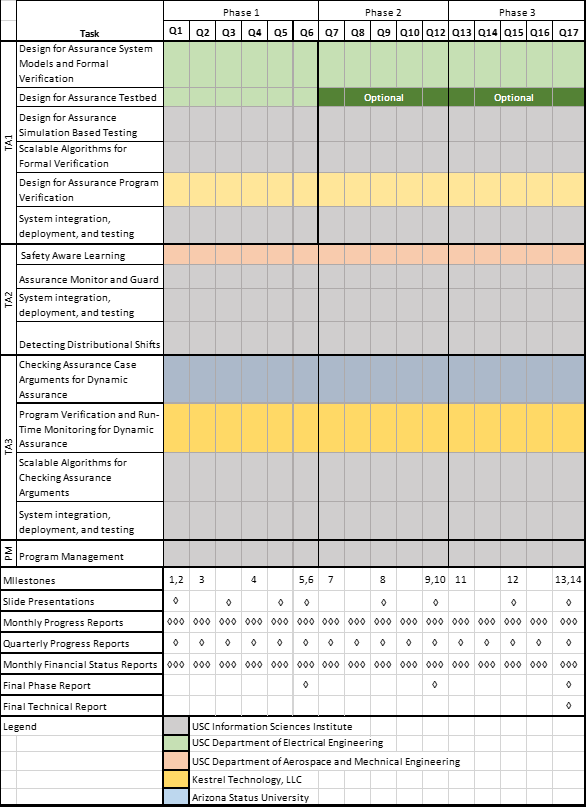
\includegraphics[width=.95\textwidth]{figs/Safeguard_Schedule_V6}
\end{center}
\vspace{-.2in}\caption{Project schedule along with a summary of milestones.  The legend maps task color to organization primary responsible for the task. } 
\label{fig:sandm}
\end{figure}
 

% \section{Level of Effort by Task \textcolor{red}{[Mike/Lisa - 1 pages]}}

% \textcolor{blue}{
% \begin{itemize}
% \item Will be a separate spreadsheet
% \item
% \end{itemize}
% }

\section*{Appendix A: Team Members and Other Information}
\addcontentsline{toc}{section}{Appendix A: Team Members and Other Information}

\baades{This section is mandatory and must include all of the following
components. If a particular subsection is not applicable, state “NONE”.}

\vspace{1ex}

\noindent
\textbf{Team Member Identification}:

\vspace{1ex}

\baades{Provide a list of all team members including the
prime, subcontractor(s), and consultant(s), as applicable. Identify specifically
whether any are a non-US organization or individual, FFRDC and/or Government
entity.}

\begin{centering}

%\small
\begin{tabular}{|p{1.8in}|p{1in}|p{1.1in}|p{0.7in}|p{0.8in}|p{0.7in}|}
\hline
 \textbf{Name} &  \textbf{Role} & \textbf{Organization} & \textbf{Non-US Org?}  & \textbf{Non-US Ind?} &  \textbf{FFRDC or Gov} \\
 \hline
Craig A. Knoblock & Prime & USC & N & N & N\\ \hline
Michael Orosz & Prime & USC & N &  N & N \\ \hline
Satish Thittamaranahalli & Prime & USC & N &  Y & N \\ \hline
Ryan Goodfellow & Prime & USC & N &  N & N \\ \hline
Anoop Kumar & Prime & USC & N & N & N \\ \hline
Satyandra Gupta & Prime & USC & N & N & N \\ \hline
Pierluigi Nuzzo & Prime & USC & N & Y & N \\ \hline
Petros Ioannou & Prime & USC & N & N & N \\ \hline
Chitta Baral & Subcontractor & ASU & N & N & N \\ \hline
Matt Barry & Subcontractor & Kestrel Technology & N & N & N \\ \hline
Douglas Smith & Subcontractor & Kestrel Technology & N & N & N \\ \hline
Henny Sipma & Subcontractor & Kestrel Technology & N & Y & N \\ \hline
\end{tabular} 
\end{centering}

\vspace{1ex}

\noindent
\textbf{Government or FFRDC Team Member Proof of Eligibility to Propose}: NONE

\baades {If
none of the team member organizations (prime or subcontractor) are a
Government entity or FFRDC, state “NONE”.}

\vspace{1ex}

\noindent
\textbf{Government or FFRDC Team Member Statement of Unique Capability}: NONE

\vspace{1ex}

\noindent
\textbf{Organizational Conflict of Interest Affirmations and Disclosure}: NONE

\vspace{1ex}

\noindent
\textbf{Intellectual Property (IP)}: 
\baades {
If no IP restrictions are intended, state “NONE”.
The Government will assume unlimited rights to all IP not explicitly identified as
having less than unlimited rights in the proposal.
For all technical data or computer software that will be furnished to the
Government with other than unlimited rights, provide (per Section VI.B.1) a list
describing all proprietary claims to results, prototypes, deliverables or systems
supporting and/or necessary for the use of the research, results, prototypes
and/or deliverables. Provide documentation proving ownership or possession of
appropriate licensing rights to all patented inventions (or inventions for which a
patent application has been filed) to be used for the proposed project.
}
\begin{centering}

%\small
\begin{tabular}{|p{2.1in}|p{1.2in}|p{1.4in}|p{2in}|}
\hline
\multicolumn{4}{|c|}{COMMERCIAL ITEMS }\\ \hline 
 \textbf{Technical Data, Computer Software To be Furnished With Restrictions} &  \textbf{Basis for Assertion} & \textbf{Asserted Rights Category} & \textbf{Name of Person Asserting Restrictions}  \\  \hline
KT Advance & Developed with mixed funding. & Restricted & David Kulich, Contracts Manager, Kestrel technology, LLC.\\ \hline
\end{tabular} 
\end{centering}

\vspace{1ex}

\noindent
\textbf{Human Subjects Research (HSR)}: NONE

\vspace{1ex}

\noindent
\textbf{Animal Use}: NONE

\vspace{1ex}

\noindent
\textbf{Representations Regarding Unpaid Delinquent Tax Liability or a Felony
Conviction under Any Federal Law}: 
%NONE

\begin{enumerate}
\item
The proposer is  not a corporation that has any unpaid Federal tax liability that has been assessed, for which all judicial and administrative remedies have been exhausted or have lapsed, and that is not being paid in a timely manner pursuant to an agreement with the authority responsible for collecting the tax liability,
\item
The proposer is not a corporation that was convicted of a felony criminal violation under a Federal law within the preceding 24 months.
\end{enumerate}

\vspace{1ex}

\noindent
\textbf{Cost Accounting Standards (CAS) Notices and Certification}:
\baades{
For any proposer who submits a proposal which, if accepted, will result in a CAS-compliant
contract, must include a Disclosure Statement as required by 48 CFR
9903.202. The disclosure forms may be found at
http://www.whitehouse.gov/omb/procurement\_casb
If this section is not applicable, state “NONE”. For further information regarding
this subject, please see www.darpa.mil/work-with-us/additional-baa.
}
NONE


%\section{Appendix B \textcolor{red}{[No Page Count]}}

\section{References}
\bibliographystyle{acm} 
\bibliography{TA3/ta3,TA2/ta2,TA1/ta1}
\end{document}
%%\documentclass[a4paper]{article}
%\documentclass[12pt]{article}
\documentclass[12pt]{dod-blank}

%% Language and font encodings
\usepackage[english]{babel}
\usepackage[utf8x]{inputenc}
\usepackage[T1]{fontenc}

%% Sets page size and margins
%%\usepackage[a4paper,top=3cm,bottom=2cm,left=3cm,right=3cm,marginparwidth=1.75cm]{geometry}
%\usepackage[top=1in, bottom=1in, left=1in, right=1in]{geometry}



%% Useful packages
\usepackage{amsmath}
\usepackage{graphicx}
  \graphicspath{{.}{./image/}}
  \DeclareGraphicsExtensions{.png,.jpg} 
\usepackage[colorinlistoftodos]{todonotes}
\usepackage[colorlinks=true, allcolors=blue]{hyperref}
\usepackage{tabularx}
\usepackage{multirow}
\usepackage{tabulary}
\usepackage{float}
\usepackage{wrapfig}
\usepackage[export]{adjustbox}
\usepackage{comment}
\usepackage{tabularx}
\usepackage{multirow}
\usepackage{tabulary}
\usepackage{enumitem}

\usepackage{listings}
\usepackage{color}
\usepackage{array}
\usepackage{subcaption}
\usepackage{xcolor}




\renewcommand{\textfraction}{0}
\renewcommand{\topfraction}{1.0}
\renewcommand{\bottomfraction}{1.0}

\usepackage{longtable}
%% macros
\newif\iffinal
\finaltrue
\iffinal
  
    \newcommand\baareq[1]{}
    \newcommand\baades[1]{}
 
 
\else
    \definecolor{darkgreen}{rgb}{0,0.4,0}
    \definecolor{darkcyan}{rgb}{0,0.4,0.4}
    \definecolor{darkblue}{rgb}{0,0,0.5}
    
    \newcommand\baareq[1]{{\color{darkcyan}[\textbf{Requirement:} #1]}}
    \newcommand\baades[1]{{\color{darkcyan}[\textbf{Description:} #1]}}
 
\fi




\def\naive{na\"{\i}ve}



\lstset{ 
  backgroundcolor=\color{white},   % choose the background color; you must add \usepackage{color} or \usepackage{xcolor}
  basicstyle=\footnotesize\ttfamily,            % the size of the fonts that are used for the code
  breakatwhitespace=false,         % sets if automatic breaks should only happen at whitespace
  breaklines=true,                 % sets automatic line breaking
  captionpos=b,                    % sets the caption-position to bottom
  commentstyle=\color{mygreen},    % comment style
  % deletekeywords={...},            % if you want to delete keywords from the given language
  escapeinside={\%*}{*)},          % if you want to add LaTeX within your code
  extendedchars=true,              % lets you use non-ASCII characters; for 8-bits encodings only, does not work with UTF-8
  frame=single,	                   % adds a frame around the code
  keepspaces=false,                 % keeps spaces in text, useful for keeping indentation of code (possibly needs columns=flexible)
  keywordstyle=\color{blue}\bfseries\underbar,       % keyword style
  language=Prolog,                 % the language of the code
  % morekeywords={if,and},        % if you want to add more keywords to the set
  numbers=none,                    % where to put the line-numbers; possible values are (none, left, right)
  numbersep=5pt,                   % how far the line-numbers are from the code
  numberstyle=\tiny\color{mygray}, % the style that is used for the line-numbers
  rulecolor=\color{black},         % if not set, the frame-color may be changed on line-breaks within not-black text
  showspaces=false,                % show spaces everywhere adding particular underscores; it overrides 'showstringspaces'
  showstringspaces=false,          % underline spaces within strings only
  showtabs=false,                  % show tabs within strings adding particular underscores
  stepnumber=2,                    % the step between two line-numbers. If it's 1, each line will be numbered
  stringstyle=\color{mymauve},     % string literal style
  tabsize=2,	                   % sets default tabsize to 2 spaces
  title=\lstname                   % show the filename of files included with \lstinputlisting; also try caption instead of title
}

% apply trick for additional keywords for our AC DSL
\lstset{
	emph={for, if, and, or},
    emphstyle={\color{blue}\bfseries\underbar}
}




\title{DARPA Assured Autonomy}
\author{Technical Volume- \textcolor{red}{Thirty-Eight (38) pages max}}

\begin{document}
\pagenumbering{roman}
 
\begin{center}
\large{\textbf{Volume 1: Technical and Management Proposal}}
\end{center}
\textbf{BAA Number:} DARPA-HR001117S0045 \\
\textbf{Technical Area:} TA1, TA2, and TA3 \\
\textbf{Proposal Title:} Assured Autonomy for Learning Enabled Vehicles (Safeguard) \\
\textbf{Lead Institution:} University of Southern California \\
\textbf{Type of organization: } “OTHER EDUCATIONAL” \\

\begin{tabularx}{\linewidth}{XX}

 \textbf{Technical Point of Contact} &  \textbf{Administrative Point of Contact }   \\
Dr.\ Craig A. Knoblock  & Sapphire Masterson  \\ 
USC Information Sciences Institute & USC Dept. of Contracts \& Grants \\
4676 Admiralty Way, Suite 1001 & 4676 Admiralty Way, Suite 1001 \\
Marina del Rey, CA 90292 & Marina del Rey, CA 90292 \\
Tel: 310-448-8786 &  Tel: (310) 448-9161 \\
E-mail: knoblock@isi.edu  & E-mail: sapphirm@usc.edu \\
\end{tabularx}
\\
\\
\textbf{Award instrument requested:}  Procurement Contract, Cost-Reimbursement, No Fee
\\
\\
\textbf{Total amount of the proposed effort:} \$ ...\\
Phase I: \$ ... \\
Phase II: \$ ... \\
Phase III: \$ ... \\
\\
\textbf{Place(s) of performance:} USC, Marina del Rey, CA; Los Angeles, CA;  Tempe, AZ; Palo Alto, CA \\
\textbf{Period(s) of performance:} 04/02/2018 - 03/31/2022     \\
\\
\textbf{Other team members:} \\
\begin{tabularx}{\linewidth}{XX}
Kestrel Technology  & Arizona State University \\
(small business) & (Other Educational)\\
POC: Matthew Barry & POC: Chitta Baral\\
3260 Hillview Avenue & Department of Computer Science and Engr. \\
Palo Alto, CA 94304 & Ira A. Fulton School of Engineering \\ 
phone: (832)205-4876 & Arizona State University\\ 
mrbarry@kestreltechnology.com & Brickyard Suite 572, 699 S. Mill Avenue \\
& Tempe, AZ 85281-8809, U.S.A.\\
& email: chitta@asu.edu\\
\end{tabularx}
\\
\textbf{Proposal validity period: } 180 days\\
\\
\textbf{Data Universal Numbering System (DUNS) number: } 072933393\\
\textbf{Taxpayer identification number:} 95-1642394\\
\textbf{Commercial and Government Entity (CAGE) code:} 1B729 Marina del Rey, CA\\
\textbf{Proposer’s reference number (if any):}  4409-0\\

\newpage
\section{Table of Contents}
\tableofcontents

\newpage
\pagenumbering{arabic}
\section{Executive Summary}
As we rapidly move into a world where machine learning plays a central role in realizing autonomous systems, it is becoming increasingly important to develop techniques that assure that these systems will operate safely and perform as expected. Current approaches are limited to providing assurance for systems with limited or no  learning capabilities. In this context, DARPA's Assured Autonomy BAA seeks to \emph{develop rigorous design and analysis technologies for continual assurance of learning-enabled autonomous systems}. USC in collaboration with Kestrel Technology and ASU is pleased to submit a comprehensive TA1, TA2, and TA3 proposal entitled \emph{``Assured Autonomy for Learning Enabled Vehicles (Safeguard).''} We plan to provide an end-to-end solution to support autonomous systems with learning-enabled components, ranging from design technologies for assurance, to assurance monitoring and control techniques, to representation and online evaluation of assurance cases. We have assembled a strong team of experts that cover the range of technologies that are required to create such an end-to-end system. If successful, the project will provide the technologies for building the next-generation of learning-enabled autonomous systems.  The entire project will take four years and cost \textcolor{red}{\$??}, with an initial version completed at the end of Phase I and successive versions with additional capabilities and improved scalability at the end of Phase II and Phase III.  

In the remainder of this section, we first introduce an  unmanned surface vehicle scenario that will be used throughout the proposal to describe the approach.  Next, we describe our approach to design, monitoring, and dynamic assurance. Finally, we introduce the team involved in the project. 

\textbf{Motivating Scenario.} Consider an autonomous unmanned surface vehicle (USV) guarding a valuable asset in the ocean when an unknown vehicle  approaches the security perimeter, under challenging weather conditions. In this scenario, the USV is required to approach the intruding vehicle, issue a warning signal, and escort it to a safe distance from the controlled area. However, as the USV has no a priori knowledge of its external environment behaviors (e.g., water depth, waves, wind, current, visibility), pre-computing a feasible trajectory, let alone optimal, becomes a non-trivial problem. For trajectory planning, the USV must continuously perform the following tasks:
\begin{itemize}[itemsep=0pt,leftmargin=*]
 \item Sense the current state of the surrounding environment (e.g., water depth, waves, wind, current, visibility) and estimate its own maneuverability constraints (e.g., braking distance, available acceleration, maximum velocity, turning radius, turning rate, safety distance) based on the state of the environment;      
\item Sense the static obstacles in the sensor range and generate a traversability map;
\item Sense the moving obstacles and classify them;   
\item Predict future trajectories of moving obstacles; 
\item Determine if any of the COLREGS \cite{commandant1999international} rules will be in effect with respect to one or more of the nearby vessels and identify the vessels with the right of way.    
\end{itemize}
The above information will be used by the trajectory planner to compute an initial trajectory, which will be continuously refined as the USV gathers additional information.
% It is not possible for the USV to be tested in every possible environment. 
The USV will use learning enabled components to take  decisions as it encounters new situations, such as  
\begin{itemize}[itemsep=0pt,leftmargin=*]
\item Classifiers to identify moving obstacles based on physical appearance and motion signatures,
\item Algorithms to estimate the sensor capabilities in adverse weather conditions,   
\item Algorithms to accurately estimate uncertainty in the environment, 
\item Classifiers to generate traversability maps,
\item Prediction of external vessel behaviors based on motion histories, 
\item Reinforcement learning  to ensure COLREGS compliance of maneuvers,  
\item Algorithms to learning pursuit behaviors.  
\end{itemize}
Learning enabled components will interact with each other in complex ways, where a misclassification error in one component may eventually compromise the entire mission.   
% We will need to make sure that each learning enabled components has a run-time monitor that will ensure that the assumptions made by the learning-enabled component remain valid and prevent erroneous learning. 
% For example, if the vehicle is exhibiting significant error in trajectory tracking, then simply downgrading the trajectory tracking error value may not be a good option.  The failure of prediction of trajectory tracking error might be due to the presence of a significant wake caused by a nearby vessel. The presence of the nearby vessel can be used to explain the degradation in trajectory tracking performance. As the vessel moves away, we can expect the trajectory tracking performance to return to the predicted level.  
While exhaustive validation of learning-enabled cyber-physical systems (LE-CPSs) is a prohibitive task~\cite{Kalra16},
their complexity, heterogeneity, and highly dynamic nature
make it challenging to even leverage existing model-based development techniques to effectively assess system correctness 
% dependability, 
at design time or enforce it at runtime.

\textbf{Design for Assurance.} Safeguard uses a platform-based design approach~\cite{Nuzzo15b} to organize the design process for a LE-CPS and to build assurance cases. Composite models are developed at several levels of abstraction,
from top-level system requirements and safety constraints down to the
implementation level.  Intermediate levels add detail to the levels
above.  The different levels are connected by refinement mappings that
allow properties established at one level to be preserved at the next
level (see Figures~\ref{fig:methodology} and~\ref{fig:assurance}).

Contracts are used to formally specify components and composite models
in terms of (1) Assumptions -- the assumed behaviors of the
environment and the behaviors of other components, and (2) Guarantees
-- the behavior properties that a model guarantees if it operates in a
context that satisfies its assumptions.  A calculus of contracts
allows horizontal composition of contracts to generate contracts for
composite models.  Vertical contracts are used to specify the mapping
or refinement relation between models at different levels of
abstraction.  The system design process starts with a high-level
contract that expresses overall system assumptions and requirements.
Subsequent levels express models with increasing detail until the
lowest level expresses the system in terms of hardware components and
their software controllers.

The assurance case for a CPS arises from the horizontal and vertical
structure of the design in several ways.  The components used within a
particular level are either (1) synthesized using
correct-by-construction design tools together with proofs, (2) derived
statically or dynamically using safety-aware machine-learning
techniques, (3) written manually and verified by analysis tools, or
(4) written manually and validated by extensive testing.  The
assurance case for the whole reflects its compositional structure.  We
anticipate that well-specified contracts together with the calculus of
contracts will eliminate well-known problems with unexpected emergent
behaviors in CPS systems.

The assurance case for the lowest-layer design arises from both the
intra-level assurance and from properties and their proofs that are
preserved under the refinement mapping from the top-level
requirements.  The refinement mappings between model layers will be
constructed using a variety of techniques.  A contract at an abstract
level can be mapped to a component or refined contract by (1)
retrieval of pre-verified components from a platform library, (2)
synthesis using correct-by-construction design and optimization tools,
or (3) manual coding to satisfy a contract.  The mapping of a
composite model will be composed from the mappings of its constituent
components or contracts.  When a composite model cannot be mapped
compositionally to the next level, it will be generated using
correct-by-construction design and optimization tools.

\textbf{Assurance Monitoring and Control.}
We provide an integrated framework for safety-aware learning, assurance monitoring and control, detecting distribution shifts. Three major components offer an efficient TA2 architecture as well as interfaces with TA1 and TA3, that is, (a) safety-aware learning and planning, (b) assurance monitors for guarding architectural and safety constraints; and (c) distribution shift detection.

We will develop a new learning-enabled online decision-making framework that allows opportunistically composing a sequence of actions (maneuvers) to reduce uncertainty in the system capability model without suspending the progress toward the mission goals or compromising safety. Each candidate action is evaluated based on three criteria: (1) the risk of violating a safety constraint using the current uncertainties in the parameter estimates; (2) its relevance to the mission goals; (3)  its expected information gain, i.e., reduction in uncertainty, with respect to the parameter estimates. These evaluations are combined to produce a cumulative mission utility value for each action that drives our learning-enabled decision-making framework. The problem of generating and evaluating sequences of actions can be posed in several way. For example, it can be solved using a branch-and-bound search method like Anytime A*, or formulated with the finite-horizon Markov Decision Process (MDP) framework. We will develop new scalable search strategies to solve this problem efficiently, by potentially evaluating a recent method developed at USC, called FastMap, that can significantly improve the execution time. 

We will develop monitors for architectural and safety constraints. 
% While these constraints can be checked over and over again as sensor information flow in, this naive strategy accounts for a lot of computational overhead. 
To achieve scalability and decrease the overhead, we propose the application of a technique that we currently use in DARPA's RSPACE program, which leverages a physical model of the vehicles dynamics and its interactions with the environment to efficiently determine the readout frequency. We propose two  extensions of this basic idea. First, we will use the theory of Variable Elimination to prioritize which variables to monitor, e.g., controllable, versus uncontrollable, adversarially controlled, or unobservable variables. Second, we invoke the dynamic assessment of assurance cases only when needed. This  decreases the number of times dynamic assessment of assurance cases is initiated as well as the communication bandwidth between the TA2 and TA3 components.

Finally, we will identify a distribution shift by combining statistical and machine learning techniques to differentiate between environmental and sensor changes. We will exploit a categorization of the shifts based on their cause and duration as well as extend our earlier work on detecting and mitigating sensor failures for all types of monitored variables.  

\textbf{Dynamic Assurance:} The Safeguard {\em design for assurance\/} activity takes a systems-theoretic stance toward safety.  Consequently, it presumes that safety is an emergent property of the system, and that hazards can present themselves through unintended interactions and performance violations in addition to causal events such as component failures.  Our design approach includes consideration of intent as well as hazard analysis and mitigation.  The artifacts from these activities populate contracts and assumptions for the dynamic assurance case.  
We thus build safety into the product by working at a systems-level viewpoint, using lexicon and design patterns familiar to both hardware and software engineers; safety is an emergent property of the system, not an afterthought.  
As system behavior evolves during runtime owing to learning, threats, degradation, or some other factor, the dynamic assurance case identifies whether the safety constraints continue to be satisfied.  If not, it provides notifications or issues recovery instructions directly from a lookup table.

Our implementation of the dynamic assurance case employs a declarative knowledge base inference engine and a domain-specific language tailored to our approach.  We have used them successfully for assurance case tool sets and arguments, and will extend them to reason about uncertainty and learning.  Our approach to achieve scalability is to specialize solvers toward modularity and to take advantage of domain knowledge.  Specifically, we will develop answer set programming techniques for context-dependent learning for reasoning about the learning-enabled components as well as learning assurance rules.  We will develop new formalisms for uncertainty to include causality, using weights for computing probabilities, and probabilistic non-monotonicity.  To achieve scaling objectives we will implement specializations using modularity, weighted CSPs, and message passing. 

% The system safety constraints revealed from that design become the key elements of our dynamic assurance case.  Our verification tools ensure the constraints are relevant, identifiable, and their implementation and effect observable.  

\textbf{Team.} We have assembled a team that is exceptionally well-qualified to build the proposed Safeguard system.  The team will be led by Dr.\ Craig Knoblock, the Principal Investigator for the effort, who currently leads the Intelligent Systems Division at the Information Sciences Institute.  He has led many large DARPA and IARPA projects over the years and has a strong track record in conducting leading edge research and then transitioning the technology to commercial use.  He will be supported by Dr.\ Michael Orosz as the Project Manager, who also has  experience in managing large research projects and on autonomous systems.  The TA1 team will be led by Dr.\ Pierluigi Nuzzo, who is an expert in embedded system design methodologies and the  application of formal methods to cyber-physical systems.  The TA1 team also includes Dr.\ Doug Smith, who has spent many years working on scalable correct-by-construction techniques and Dr.\ Henny Sipma, who has significant experience in applying program verification methods to real-world problems.  The TA1 team also includes Ryan Goodfellow, who has done a large amount of work on simulation-based testing.  The TA2 team will be led by Dr.\ Knoblock who has worked on topics related to both monitoring and detecting distribution changes.  He will be supported by Dr.\ Satyandra Gupta, who is an expert on autonomous surface vehicles as well as on safety-aware learning. He will also be supported by Drs.\ Anoop Kumar and Satish Thittamaranahalli, who have also previously worked on efficient methods for execution monitoring.  The TA3 team will be lead by Dr.\ Matthew Barry, who has experience in creating the technologies for assurance cases.  He will be supported by Dr.\ Chitta Baral, who is an expert on ASP solvers and by Dr.\ Thittamaranahalli who is an expert on SAT solvers, both of which will be applied to provide scalable assurance case reasoning.  Finally, Dr.\ Petros Ioannou, who is an expert on control systems for autonomous vehicles will provide an autonomous vehicle platform, which will form the focus of our work until the TA4 teams provide additional vehicle platforms for development.  

\newpage
\section{Innovative Claims and Deliverables}

In this project we will develop and build an end-to-end system for assured autonomy.  This section describes the key innovations by technical area and then the overall deliverables of the project.

\paragraph{Design for Assurance}

\begin{itemize}[itemsep=0pt,leftmargin=*]
\item We address the LE-CPS design challenges via a holistic approach that can contextually generate design artifacts and assurance cases. We develop a compositional, contract-based modeling framework, methods, and tools to support the design process from system-level requirement capture,  formalization, and analysis, to the generation, testing, and continual monitoring of software and hardware artifacts in feedback loop with a physical process.

\item We develop compositional abstractions and interfaces (vertical contracts) that can  bridge heterogeneous formalisms and heterogeneous decomposition architectures to make system analysis and synthesis tractable, consistently combine different verification and synthesis methods at design time, and provide seamless support for dynamic assurance at run time. %We aim to quantitatively capture the confidence in the satisfaction of requirements under uncertain or unknown conditions, and resilience properties of  systems at different abstraction levels, to enable trade-off evaluation between resilience, performance, and cost.

\item We develop a unifying framework and efficient algorithms to reason about the combination of discrete and continuous dynamics and constraints in the presence of uncertainties in LE-CPS using a satisfiability modulo convex approach~\cite{Shoukry2017} for contract-based system verification and scalable trajectory planning.  

\item We provide an environment for high-fidelity CPS testing, in which production-ready software, e.g.,  safety-critical learning and control, may be deployed and tested 
% by extending the Cypress testbed environment \cite{Goodfellow2015Cypress:Systems} 
with time dilation facilities, so that it synchronizes with a physical simulation that is not necessarily running in real time, while still having the perception of real time.

\item We 
% These facilities allow a cyber system to be  
propose an approach for unanticipated behavior space identification and test coverage maximization which leverages results from the theory of differential algebraic equation (DAE)~\cite{Berger2013ControllabilitySurvey,Ilchmann2005ATheory,BergerOnSystems,Lamour2013} 
to prune the behavior search space and identify smaller regions of interest for efficient simulation-based testing. 
% We then compute the intersection of these two behavior spaces and restrict our simulation based testing search space to this subspace.
\end{itemize}

\paragraph{Assurance Monitoring and Control}

\begin{itemize}[itemsep=0pt,leftmargin=*]
\item 
%We integrate safety-aware learning into the overall decision making problem. The goal is to maximize mission utility without violating the safety constraints. 
Our safety-aware learning framework enables the system to opportunistically select and execute actions to assist the learning-enabled component in reducing model uncertainty without compromising safety or deviating from the mission goals. The value of uncertainty reduction is explicitly incorporated in the optimization process for selecting the best action.  
\item For safety-aware learning, we propose the idea of preprocessing the search space of the problem domain before queries and observations come in. With such a linear-time preprocessing phase, the performance of search and optimization algorithms can be significantly boosted. For example, in regular A* search, the intensional or extensional search space can be preprocessed in near-linear time to yield an embedding of each state as a point in Euclidean space~\cite{cujakk}. Then, when the query comes in, A* search can make use of these Euclidean distances as heuristic distances between two states to yield order-of-magnitude speedups. 
%In Anytime A* for safety-aware learning and planning, this leads to a significantly better quality of actions chosen within a time limit, and in the MDP framework, the same ideas can be used to improve the convergence of Bellman updates for safety-aware Reinforcement Learning.
\item As massive amounts of sensor information flow in, it is imperative for us to efficiently process this information for monitoring architectural and safety constraints. Building on our past work on similar tasks, we propose novel technologies for efficiently monitoring constraints. These algorithms can yield an exponential reduction in the amount of sensor data that needs to be processed. Doing this also reduces the message complexities between the various modules. %We also propose to use the theory of Variable Elimination (VE) to monitor constraints with uncontrollable, adversarially controlled, and/or unobservable variables. VE yields a substrate constraint to monitor that characterizes a dominant strategy of the controllable variables over the uncontrollable, adversarially controlled, and/or unobservable variables.
\item We will develop techniques to identify  distributional shifts and determine the underlying cause (e.g., change in environment, sensor failure,   etc.), as well as strategies for handling the various distributional shifts.   Notably, we propose to build on our past work and use compact representations to exploit historical data to identify distributional shifts.
\end{itemize}

\paragraph{Dynamic Assurance}

\begin{itemize}[itemsep=0pt,leftmargin=*]

\item We demonstrate the integration of dynamic assurance for safety-critical learning-enabled dynamic systems in which evolutionary behaviors are expected and tolerated as a property of the functionality.   The impact will be consequential contributions safety-critical dynamic systems in which evolutionary behaviors are expected and tolerated as portion of the functionality.   
\item We implement dynamic assurance by combining features of system safety, formal methods, logic programming, uncertain reasoning, and domain-specific languages.  We populate assurance case arguments at several levels of modeling and implementation abstraction, using the analysis results to produce design-time evidence supporting assurance claims.  
%We provide automated reasoning about the assurance case itself to produce verification, consistency, and completeness results for the argument.  Dynamic assurance results then yield trusted explanations of whether safety constraints and assumptions and other contracts still hold during the collection of runtime evidence from monitors. 
\item We develop and demonstrate ASP formalisms crucial to applications in dynamic assurance. We demonstrate the suitability of the technology especially for assurance case arguments owing to the improved legibility, consistency and completeness checks, handling of uncertain and default reasoning, and scalability.  
%We will produce modularized solvers for enhanced performance based on recent algorithmic developments in exploiting structure, kernelization, and message passing. We provide a formalism to enable learning of assurance rules. 
We provide a novel approach to handling uncertainty that provides the ability to do causal and counter-factual reasoning as well as probabilistic non-monotonicity.  Overcoming limitations of traditional inductive logic techniques, we develop a novel iterative and incremental approach based on context dependent learning. 
\end{itemize}

\paragraph{Deliverables}
During the course of this project, we will build and deliver a fully-operational system that covers all three of the technical areas.  The detailed capabilities of this system are described in the individual technical sections.  The resulting system will be available as open source under a permissive license, which will allow other organizations to use the work, extend it in new directions, and even commercialize the software.  Kestrel Technology has significant experience in this space and has built and applied these types of technologies to a variety of real world tasks.  Kestrel is ideally suited to pursue commercial uses of this technology and the permissive license will facilitate exploring these opportunities since there will be no need to negotiate intellectual property rights.  

\newpage
\section{Technical Plan}
%%\documentclass[a4paper]{article}
%\documentclass[12pt]{article}
\documentclass[12pt]{dod-blank}

%% Language and font encodings
\usepackage[english]{babel}
\usepackage[utf8x]{inputenc}
\usepackage[T1]{fontenc}

%% Sets page size and margins
%%\usepackage[a4paper,top=3cm,bottom=2cm,left=3cm,right=3cm,marginparwidth=1.75cm]{geometry}
%\usepackage[top=1in, bottom=1in, left=1in, right=1in]{geometry}



%% Useful packages
\usepackage{amsmath}
\usepackage{graphicx}
  \graphicspath{{.}{./image/}}
  \DeclareGraphicsExtensions{.png,.jpg} 
\usepackage[colorinlistoftodos]{todonotes}
\usepackage[colorlinks=true, allcolors=blue]{hyperref}
\usepackage{tabularx}
\usepackage{multirow}
\usepackage{tabulary}
\usepackage{float}
\usepackage{wrapfig}
\usepackage[export]{adjustbox}
\usepackage{comment}
\usepackage{tabularx}
\usepackage{multirow}
\usepackage{tabulary}
\usepackage{enumitem}

\usepackage{listings}
\usepackage{color}
\usepackage{array}
\usepackage{subcaption}
\usepackage{xcolor}




\renewcommand{\textfraction}{0}
\renewcommand{\topfraction}{1.0}
\renewcommand{\bottomfraction}{1.0}

\usepackage{longtable}
%% macros
\newif\iffinal
\finaltrue
\iffinal
  
    \newcommand\baareq[1]{}
    \newcommand\baades[1]{}
 
 
\else
    \definecolor{darkgreen}{rgb}{0,0.4,0}
    \definecolor{darkcyan}{rgb}{0,0.4,0.4}
    \definecolor{darkblue}{rgb}{0,0,0.5}
    
    \newcommand\baareq[1]{{\color{darkcyan}[\textbf{Requirement:} #1]}}
    \newcommand\baades[1]{{\color{darkcyan}[\textbf{Description:} #1]}}
 
\fi




\def\naive{na\"{\i}ve}



\lstset{ 
  backgroundcolor=\color{white},   % choose the background color; you must add \usepackage{color} or \usepackage{xcolor}
  basicstyle=\footnotesize\ttfamily,            % the size of the fonts that are used for the code
  breakatwhitespace=false,         % sets if automatic breaks should only happen at whitespace
  breaklines=true,                 % sets automatic line breaking
  captionpos=b,                    % sets the caption-position to bottom
  commentstyle=\color{mygreen},    % comment style
  % deletekeywords={...},            % if you want to delete keywords from the given language
  escapeinside={\%*}{*)},          % if you want to add LaTeX within your code
  extendedchars=true,              % lets you use non-ASCII characters; for 8-bits encodings only, does not work with UTF-8
  frame=single,	                   % adds a frame around the code
  keepspaces=false,                 % keeps spaces in text, useful for keeping indentation of code (possibly needs columns=flexible)
  keywordstyle=\color{blue}\bfseries\underbar,       % keyword style
  language=Prolog,                 % the language of the code
  % morekeywords={if,and},        % if you want to add more keywords to the set
  numbers=none,                    % where to put the line-numbers; possible values are (none, left, right)
  numbersep=5pt,                   % how far the line-numbers are from the code
  numberstyle=\tiny\color{mygray}, % the style that is used for the line-numbers
  rulecolor=\color{black},         % if not set, the frame-color may be changed on line-breaks within not-black text
  showspaces=false,                % show spaces everywhere adding particular underscores; it overrides 'showstringspaces'
  showstringspaces=false,          % underline spaces within strings only
  showtabs=false,                  % show tabs within strings adding particular underscores
  stepnumber=2,                    % the step between two line-numbers. If it's 1, each line will be numbered
  stringstyle=\color{mymauve},     % string literal style
  tabsize=2,	                   % sets default tabsize to 2 spaces
  title=\lstname                   % show the filename of files included with \lstinputlisting; also try caption instead of title
}

% apply trick for additional keywords for our AC DSL
\lstset{
	emph={for, if, and, or},
    emphstyle={\color{blue}\bfseries\underbar}
}




\title{DARPA Assured Autonomy}
\author{Technical Volume- \textcolor{red}{Thirty-Eight (38) pages max}}

\begin{document}
\pagenumbering{roman}
 
\begin{center}
\large{\textbf{Volume 1: Technical and Management Proposal}}
\end{center}
\textbf{BAA Number:} DARPA-HR001117S0045 \\
\textbf{Technical Area:} TA1, TA2, and TA3 \\
\textbf{Proposal Title:} Assured Autonomy for Learning Enabled Vehicles (Safeguard) \\
\textbf{Lead Institution:} University of Southern California \\
\textbf{Type of organization: } “OTHER EDUCATIONAL” \\

\begin{tabularx}{\linewidth}{XX}

 \textbf{Technical Point of Contact} &  \textbf{Administrative Point of Contact }   \\
Dr.\ Craig A. Knoblock  & Sapphire Masterson  \\ 
USC Information Sciences Institute & USC Dept. of Contracts \& Grants \\
4676 Admiralty Way, Suite 1001 & 4676 Admiralty Way, Suite 1001 \\
Marina del Rey, CA 90292 & Marina del Rey, CA 90292 \\
Tel: 310-448-8786 &  Tel: (310) 448-9161 \\
E-mail: knoblock@isi.edu  & E-mail: sapphirm@usc.edu \\
\end{tabularx}
\\
\\
\textbf{Award instrument requested:}  Procurement Contract, Cost-Reimbursement, No Fee
\\
\\
\textbf{Total amount of the proposed effort:} \$ ...\\
Phase I: \$ ... \\
Phase II: \$ ... \\
Phase III: \$ ... \\
\\
\textbf{Place(s) of performance:} USC, Marina del Rey, CA; Los Angeles, CA;  Tempe, AZ; Palo Alto, CA \\
\textbf{Period(s) of performance:} 04/02/2018 - 03/31/2022     \\
\\
\textbf{Other team members:} \\
\begin{tabularx}{\linewidth}{XX}
Kestrel Technology  & Arizona State University \\
(small business) & (Other Educational)\\
POC: Matthew Barry & POC: Chitta Baral\\
3260 Hillview Avenue & Department of Computer Science and Engr. \\
Palo Alto, CA 94304 & Ira A. Fulton School of Engineering \\ 
phone: (832)205-4876 & Arizona State University\\ 
mrbarry@kestreltechnology.com & Brickyard Suite 572, 699 S. Mill Avenue \\
& Tempe, AZ 85281-8809, U.S.A.\\
& email: chitta@asu.edu\\
\end{tabularx}
\\
\textbf{Proposal validity period: } 180 days\\
\\
\textbf{Data Universal Numbering System (DUNS) number: } 072933393\\
\textbf{Taxpayer identification number:} 95-1642394\\
\textbf{Commercial and Government Entity (CAGE) code:} 1B729 Marina del Rey, CA\\
\textbf{Proposer’s reference number (if any):}  4409-0\\

\newpage
\section{Table of Contents}
\tableofcontents

\newpage
\pagenumbering{arabic}
\section{Executive Summary}
As we rapidly move into a world where machine learning plays a central role in realizing autonomous systems, it is becoming increasingly important to develop techniques that assure that these systems will operate safely and perform as expected. Current approaches are limited to providing assurance for systems with limited or no  learning capabilities. In this context, DARPA's Assured Autonomy BAA seeks to \emph{develop rigorous design and analysis technologies for continual assurance of learning-enabled autonomous systems}. USC in collaboration with Kestrel Technology and ASU is pleased to submit a comprehensive TA1, TA2, and TA3 proposal entitled \emph{``Assured Autonomy for Learning Enabled Vehicles (Safeguard).''} We plan to provide an end-to-end solution to support autonomous systems with learning-enabled components, ranging from design technologies for assurance, to assurance monitoring and control techniques, to representation and online evaluation of assurance cases. We have assembled a strong team of experts that cover the range of technologies that are required to create such an end-to-end system. If successful, the project will provide the technologies for building the next-generation of learning-enabled autonomous systems.  The entire project will take four years and cost \textcolor{red}{\$??}, with an initial version completed at the end of Phase I and successive versions with additional capabilities and improved scalability at the end of Phase II and Phase III.  

In the remainder of this section, we first introduce an  unmanned surface vehicle scenario that will be used throughout the proposal to describe the approach.  Next, we describe our approach to design, monitoring, and dynamic assurance. Finally, we introduce the team involved in the project. 

\textbf{Motivating Scenario.} Consider an autonomous unmanned surface vehicle (USV) guarding a valuable asset in the ocean when an unknown vehicle  approaches the security perimeter, under challenging weather conditions. In this scenario, the USV is required to approach the intruding vehicle, issue a warning signal, and escort it to a safe distance from the controlled area. However, as the USV has no a priori knowledge of its external environment behaviors (e.g., water depth, waves, wind, current, visibility), pre-computing a feasible trajectory, let alone optimal, becomes a non-trivial problem. For trajectory planning, the USV must continuously perform the following tasks:
\begin{itemize}[itemsep=0pt,leftmargin=*]
 \item Sense the current state of the surrounding environment (e.g., water depth, waves, wind, current, visibility) and estimate its own maneuverability constraints (e.g., braking distance, available acceleration, maximum velocity, turning radius, turning rate, safety distance) based on the state of the environment;      
\item Sense the static obstacles in the sensor range and generate a traversability map;
\item Sense the moving obstacles and classify them;   
\item Predict future trajectories of moving obstacles; 
\item Determine if any of the COLREGS \cite{commandant1999international} rules will be in effect with respect to one or more of the nearby vessels and identify the vessels with the right of way.    
\end{itemize}
The above information will be used by the trajectory planner to compute an initial trajectory, which will be continuously refined as the USV gathers additional information.
% It is not possible for the USV to be tested in every possible environment. 
The USV will use learning enabled components to take  decisions as it encounters new situations, such as  
\begin{itemize}[itemsep=0pt,leftmargin=*]
\item Classifiers to identify moving obstacles based on physical appearance and motion signatures,
\item Algorithms to estimate the sensor capabilities in adverse weather conditions,   
\item Algorithms to accurately estimate uncertainty in the environment, 
\item Classifiers to generate traversability maps,
\item Prediction of external vessel behaviors based on motion histories, 
\item Reinforcement learning  to ensure COLREGS compliance of maneuvers,  
\item Algorithms to learning pursuit behaviors.  
\end{itemize}
Learning enabled components will interact with each other in complex ways, where a misclassification error in one component may eventually compromise the entire mission.   
% We will need to make sure that each learning enabled components has a run-time monitor that will ensure that the assumptions made by the learning-enabled component remain valid and prevent erroneous learning. 
% For example, if the vehicle is exhibiting significant error in trajectory tracking, then simply downgrading the trajectory tracking error value may not be a good option.  The failure of prediction of trajectory tracking error might be due to the presence of a significant wake caused by a nearby vessel. The presence of the nearby vessel can be used to explain the degradation in trajectory tracking performance. As the vessel moves away, we can expect the trajectory tracking performance to return to the predicted level.  
While exhaustive validation of learning-enabled cyber-physical systems (LE-CPSs) is a prohibitive task~\cite{Kalra16},
their complexity, heterogeneity, and highly dynamic nature
make it challenging to even leverage existing model-based development techniques to effectively assess system correctness 
% dependability, 
at design time or enforce it at runtime.

\textbf{Design for Assurance.} Safeguard uses a platform-based design approach~\cite{Nuzzo15b} to organize the design process for a LE-CPS and to build assurance cases. Composite models are developed at several levels of abstraction,
from top-level system requirements and safety constraints down to the
implementation level.  Intermediate levels add detail to the levels
above.  The different levels are connected by refinement mappings that
allow properties established at one level to be preserved at the next
level (see Figures~\ref{fig:methodology} and~\ref{fig:assurance}).

Contracts are used to formally specify components and composite models
in terms of (1) Assumptions -- the assumed behaviors of the
environment and the behaviors of other components, and (2) Guarantees
-- the behavior properties that a model guarantees if it operates in a
context that satisfies its assumptions.  A calculus of contracts
allows horizontal composition of contracts to generate contracts for
composite models.  Vertical contracts are used to specify the mapping
or refinement relation between models at different levels of
abstraction.  The system design process starts with a high-level
contract that expresses overall system assumptions and requirements.
Subsequent levels express models with increasing detail until the
lowest level expresses the system in terms of hardware components and
their software controllers.

The assurance case for a CPS arises from the horizontal and vertical
structure of the design in several ways.  The components used within a
particular level are either (1) synthesized using
correct-by-construction design tools together with proofs, (2) derived
statically or dynamically using safety-aware machine-learning
techniques, (3) written manually and verified by analysis tools, or
(4) written manually and validated by extensive testing.  The
assurance case for the whole reflects its compositional structure.  We
anticipate that well-specified contracts together with the calculus of
contracts will eliminate well-known problems with unexpected emergent
behaviors in CPS systems.

The assurance case for the lowest-layer design arises from both the
intra-level assurance and from properties and their proofs that are
preserved under the refinement mapping from the top-level
requirements.  The refinement mappings between model layers will be
constructed using a variety of techniques.  A contract at an abstract
level can be mapped to a component or refined contract by (1)
retrieval of pre-verified components from a platform library, (2)
synthesis using correct-by-construction design and optimization tools,
or (3) manual coding to satisfy a contract.  The mapping of a
composite model will be composed from the mappings of its constituent
components or contracts.  When a composite model cannot be mapped
compositionally to the next level, it will be generated using
correct-by-construction design and optimization tools.

\textbf{Assurance Monitoring and Control.}
We provide an integrated framework for safety-aware learning, assurance monitoring and control, detecting distribution shifts. Three major components offer an efficient TA2 architecture as well as interfaces with TA1 and TA3, that is, (a) safety-aware learning and planning, (b) assurance monitors for guarding architectural and safety constraints; and (c) distribution shift detection.

We will develop a new learning-enabled online decision-making framework that allows opportunistically composing a sequence of actions (maneuvers) to reduce uncertainty in the system capability model without suspending the progress toward the mission goals or compromising safety. Each candidate action is evaluated based on three criteria: (1) the risk of violating a safety constraint using the current uncertainties in the parameter estimates; (2) its relevance to the mission goals; (3)  its expected information gain, i.e., reduction in uncertainty, with respect to the parameter estimates. These evaluations are combined to produce a cumulative mission utility value for each action that drives our learning-enabled decision-making framework. The problem of generating and evaluating sequences of actions can be posed in several way. For example, it can be solved using a branch-and-bound search method like Anytime A*, or formulated with the finite-horizon Markov Decision Process (MDP) framework. We will develop new scalable search strategies to solve this problem efficiently, by potentially evaluating a recent method developed at USC, called FastMap, that can significantly improve the execution time. 

We will develop monitors for architectural and safety constraints. 
% While these constraints can be checked over and over again as sensor information flow in, this naive strategy accounts for a lot of computational overhead. 
To achieve scalability and decrease the overhead, we propose the application of a technique that we currently use in DARPA's RSPACE program, which leverages a physical model of the vehicles dynamics and its interactions with the environment to efficiently determine the readout frequency. We propose two  extensions of this basic idea. First, we will use the theory of Variable Elimination to prioritize which variables to monitor, e.g., controllable, versus uncontrollable, adversarially controlled, or unobservable variables. Second, we invoke the dynamic assessment of assurance cases only when needed. This  decreases the number of times dynamic assessment of assurance cases is initiated as well as the communication bandwidth between the TA2 and TA3 components.

Finally, we will identify a distribution shift by combining statistical and machine learning techniques to differentiate between environmental and sensor changes. We will exploit a categorization of the shifts based on their cause and duration as well as extend our earlier work on detecting and mitigating sensor failures for all types of monitored variables.  

\textbf{Dynamic Assurance:} The Safeguard {\em design for assurance\/} activity takes a systems-theoretic stance toward safety.  Consequently, it presumes that safety is an emergent property of the system, and that hazards can present themselves through unintended interactions and performance violations in addition to causal events such as component failures.  Our design approach includes consideration of intent as well as hazard analysis and mitigation.  The artifacts from these activities populate contracts and assumptions for the dynamic assurance case.  
We thus build safety into the product by working at a systems-level viewpoint, using lexicon and design patterns familiar to both hardware and software engineers; safety is an emergent property of the system, not an afterthought.  
As system behavior evolves during runtime owing to learning, threats, degradation, or some other factor, the dynamic assurance case identifies whether the safety constraints continue to be satisfied.  If not, it provides notifications or issues recovery instructions directly from a lookup table.

Our implementation of the dynamic assurance case employs a declarative knowledge base inference engine and a domain-specific language tailored to our approach.  We have used them successfully for assurance case tool sets and arguments, and will extend them to reason about uncertainty and learning.  Our approach to achieve scalability is to specialize solvers toward modularity and to take advantage of domain knowledge.  Specifically, we will develop answer set programming techniques for context-dependent learning for reasoning about the learning-enabled components as well as learning assurance rules.  We will develop new formalisms for uncertainty to include causality, using weights for computing probabilities, and probabilistic non-monotonicity.  To achieve scaling objectives we will implement specializations using modularity, weighted CSPs, and message passing. 

% The system safety constraints revealed from that design become the key elements of our dynamic assurance case.  Our verification tools ensure the constraints are relevant, identifiable, and their implementation and effect observable.  

\textbf{Team.} We have assembled a team that is exceptionally well-qualified to build the proposed Safeguard system.  The team will be led by Dr.\ Craig Knoblock, the Principal Investigator for the effort, who currently leads the Intelligent Systems Division at the Information Sciences Institute.  He has led many large DARPA and IARPA projects over the years and has a strong track record in conducting leading edge research and then transitioning the technology to commercial use.  He will be supported by Dr.\ Michael Orosz as the Project Manager, who also has  experience in managing large research projects and on autonomous systems.  The TA1 team will be led by Dr.\ Pierluigi Nuzzo, who is an expert in embedded system design methodologies and the  application of formal methods to cyber-physical systems.  The TA1 team also includes Dr.\ Doug Smith, who has spent many years working on scalable correct-by-construction techniques and Dr.\ Henny Sipma, who has significant experience in applying program verification methods to real-world problems.  The TA1 team also includes Ryan Goodfellow, who has done a large amount of work on simulation-based testing.  The TA2 team will be led by Dr.\ Knoblock who has worked on topics related to both monitoring and detecting distribution changes.  He will be supported by Dr.\ Satyandra Gupta, who is an expert on autonomous surface vehicles as well as on safety-aware learning. He will also be supported by Drs.\ Anoop Kumar and Satish Thittamaranahalli, who have also previously worked on efficient methods for execution monitoring.  The TA3 team will be lead by Dr.\ Matthew Barry, who has experience in creating the technologies for assurance cases.  He will be supported by Dr.\ Chitta Baral, who is an expert on ASP solvers and by Dr.\ Thittamaranahalli who is an expert on SAT solvers, both of which will be applied to provide scalable assurance case reasoning.  Finally, Dr.\ Petros Ioannou, who is an expert on control systems for autonomous vehicles will provide an autonomous vehicle platform, which will form the focus of our work until the TA4 teams provide additional vehicle platforms for development.  

\newpage
\section{Innovative Claims and Deliverables}

In this project we will develop and build an end-to-end system for assured autonomy.  This section describes the key innovations by technical area and then the overall deliverables of the project.

\paragraph{Design for Assurance}

\begin{itemize}[itemsep=0pt,leftmargin=*]
\item We address the LE-CPS design challenges via a holistic approach that can contextually generate design artifacts and assurance cases. We develop a compositional, contract-based modeling framework, methods, and tools to support the design process from system-level requirement capture,  formalization, and analysis, to the generation, testing, and continual monitoring of software and hardware artifacts in feedback loop with a physical process.

\item We develop compositional abstractions and interfaces (vertical contracts) that can  bridge heterogeneous formalisms and heterogeneous decomposition architectures to make system analysis and synthesis tractable, consistently combine different verification and synthesis methods at design time, and provide seamless support for dynamic assurance at run time. %We aim to quantitatively capture the confidence in the satisfaction of requirements under uncertain or unknown conditions, and resilience properties of  systems at different abstraction levels, to enable trade-off evaluation between resilience, performance, and cost.

\item We develop a unifying framework and efficient algorithms to reason about the combination of discrete and continuous dynamics and constraints in the presence of uncertainties in LE-CPS using a satisfiability modulo convex approach~\cite{Shoukry2017} for contract-based system verification and scalable trajectory planning.  

\item We provide an environment for high-fidelity CPS testing, in which production-ready software, e.g.,  safety-critical learning and control, may be deployed and tested 
% by extending the Cypress testbed environment \cite{Goodfellow2015Cypress:Systems} 
with time dilation facilities, so that it synchronizes with a physical simulation that is not necessarily running in real time, while still having the perception of real time.

\item We 
% These facilities allow a cyber system to be  
propose an approach for unanticipated behavior space identification and test coverage maximization which leverages results from the theory of differential algebraic equation (DAE)~\cite{Berger2013ControllabilitySurvey,Ilchmann2005ATheory,BergerOnSystems,Lamour2013} 
to prune the behavior search space and identify smaller regions of interest for efficient simulation-based testing. 
% We then compute the intersection of these two behavior spaces and restrict our simulation based testing search space to this subspace.
\end{itemize}

\paragraph{Assurance Monitoring and Control}

\begin{itemize}[itemsep=0pt,leftmargin=*]
\item 
%We integrate safety-aware learning into the overall decision making problem. The goal is to maximize mission utility without violating the safety constraints. 
Our safety-aware learning framework enables the system to opportunistically select and execute actions to assist the learning-enabled component in reducing model uncertainty without compromising safety or deviating from the mission goals. The value of uncertainty reduction is explicitly incorporated in the optimization process for selecting the best action.  
\item For safety-aware learning, we propose the idea of preprocessing the search space of the problem domain before queries and observations come in. With such a linear-time preprocessing phase, the performance of search and optimization algorithms can be significantly boosted. For example, in regular A* search, the intensional or extensional search space can be preprocessed in near-linear time to yield an embedding of each state as a point in Euclidean space~\cite{cujakk}. Then, when the query comes in, A* search can make use of these Euclidean distances as heuristic distances between two states to yield order-of-magnitude speedups. 
%In Anytime A* for safety-aware learning and planning, this leads to a significantly better quality of actions chosen within a time limit, and in the MDP framework, the same ideas can be used to improve the convergence of Bellman updates for safety-aware Reinforcement Learning.
\item As massive amounts of sensor information flow in, it is imperative for us to efficiently process this information for monitoring architectural and safety constraints. Building on our past work on similar tasks, we propose novel technologies for efficiently monitoring constraints. These algorithms can yield an exponential reduction in the amount of sensor data that needs to be processed. Doing this also reduces the message complexities between the various modules. %We also propose to use the theory of Variable Elimination (VE) to monitor constraints with uncontrollable, adversarially controlled, and/or unobservable variables. VE yields a substrate constraint to monitor that characterizes a dominant strategy of the controllable variables over the uncontrollable, adversarially controlled, and/or unobservable variables.
\item We will develop techniques to identify  distributional shifts and determine the underlying cause (e.g., change in environment, sensor failure,   etc.), as well as strategies for handling the various distributional shifts.   Notably, we propose to build on our past work and use compact representations to exploit historical data to identify distributional shifts.
\end{itemize}

\paragraph{Dynamic Assurance}

\begin{itemize}[itemsep=0pt,leftmargin=*]

\item We demonstrate the integration of dynamic assurance for safety-critical learning-enabled dynamic systems in which evolutionary behaviors are expected and tolerated as a property of the functionality.   The impact will be consequential contributions safety-critical dynamic systems in which evolutionary behaviors are expected and tolerated as portion of the functionality.   
\item We implement dynamic assurance by combining features of system safety, formal methods, logic programming, uncertain reasoning, and domain-specific languages.  We populate assurance case arguments at several levels of modeling and implementation abstraction, using the analysis results to produce design-time evidence supporting assurance claims.  
%We provide automated reasoning about the assurance case itself to produce verification, consistency, and completeness results for the argument.  Dynamic assurance results then yield trusted explanations of whether safety constraints and assumptions and other contracts still hold during the collection of runtime evidence from monitors. 
\item We develop and demonstrate ASP formalisms crucial to applications in dynamic assurance. We demonstrate the suitability of the technology especially for assurance case arguments owing to the improved legibility, consistency and completeness checks, handling of uncertain and default reasoning, and scalability.  
%We will produce modularized solvers for enhanced performance based on recent algorithmic developments in exploiting structure, kernelization, and message passing. We provide a formalism to enable learning of assurance rules. 
We provide a novel approach to handling uncertainty that provides the ability to do causal and counter-factual reasoning as well as probabilistic non-monotonicity.  Overcoming limitations of traditional inductive logic techniques, we develop a novel iterative and incremental approach based on context dependent learning. 
\end{itemize}

\paragraph{Deliverables}
During the course of this project, we will build and deliver a fully-operational system that covers all three of the technical areas.  The detailed capabilities of this system are described in the individual technical sections.  The resulting system will be available as open source under a permissive license, which will allow other organizations to use the work, extend it in new directions, and even commercialize the software.  Kestrel Technology has significant experience in this space and has built and applied these types of technologies to a variety of real world tasks.  Kestrel is ideally suited to pursue commercial uses of this technology and the permissive license will facilitate exploring these opportunities since there will be no need to negotiate intellectual property rights.  

\newpage
\section{Technical Plan}
%%\documentclass[a4paper]{article}
%\documentclass[12pt]{article}
\documentclass[12pt]{dod-blank}

%% Language and font encodings
\usepackage[english]{babel}
\usepackage[utf8x]{inputenc}
\usepackage[T1]{fontenc}

%% Sets page size and margins
%%\usepackage[a4paper,top=3cm,bottom=2cm,left=3cm,right=3cm,marginparwidth=1.75cm]{geometry}
%\usepackage[top=1in, bottom=1in, left=1in, right=1in]{geometry}



%% Useful packages
\usepackage{amsmath}
\usepackage{graphicx}
  \graphicspath{{.}{./image/}}
  \DeclareGraphicsExtensions{.png,.jpg} 
\usepackage[colorinlistoftodos]{todonotes}
\usepackage[colorlinks=true, allcolors=blue]{hyperref}
\usepackage{tabularx}
\usepackage{multirow}
\usepackage{tabulary}
\usepackage{float}
\usepackage{wrapfig}
\usepackage[export]{adjustbox}
\usepackage{comment}
\usepackage{tabularx}
\usepackage{multirow}
\usepackage{tabulary}
\usepackage{enumitem}

\usepackage{listings}
\usepackage{color}
\usepackage{array}
\usepackage{subcaption}
\usepackage{xcolor}




\renewcommand{\textfraction}{0}
\renewcommand{\topfraction}{1.0}
\renewcommand{\bottomfraction}{1.0}

\usepackage{longtable}
%% macros
\newif\iffinal
\finaltrue
\iffinal
  
    \newcommand\baareq[1]{}
    \newcommand\baades[1]{}
 
 
\else
    \definecolor{darkgreen}{rgb}{0,0.4,0}
    \definecolor{darkcyan}{rgb}{0,0.4,0.4}
    \definecolor{darkblue}{rgb}{0,0,0.5}
    
    \newcommand\baareq[1]{{\color{darkcyan}[\textbf{Requirement:} #1]}}
    \newcommand\baades[1]{{\color{darkcyan}[\textbf{Description:} #1]}}
 
\fi




\def\naive{na\"{\i}ve}



\lstset{ 
  backgroundcolor=\color{white},   % choose the background color; you must add \usepackage{color} or \usepackage{xcolor}
  basicstyle=\footnotesize\ttfamily,            % the size of the fonts that are used for the code
  breakatwhitespace=false,         % sets if automatic breaks should only happen at whitespace
  breaklines=true,                 % sets automatic line breaking
  captionpos=b,                    % sets the caption-position to bottom
  commentstyle=\color{mygreen},    % comment style
  % deletekeywords={...},            % if you want to delete keywords from the given language
  escapeinside={\%*}{*)},          % if you want to add LaTeX within your code
  extendedchars=true,              % lets you use non-ASCII characters; for 8-bits encodings only, does not work with UTF-8
  frame=single,	                   % adds a frame around the code
  keepspaces=false,                 % keeps spaces in text, useful for keeping indentation of code (possibly needs columns=flexible)
  keywordstyle=\color{blue}\bfseries\underbar,       % keyword style
  language=Prolog,                 % the language of the code
  % morekeywords={if,and},        % if you want to add more keywords to the set
  numbers=none,                    % where to put the line-numbers; possible values are (none, left, right)
  numbersep=5pt,                   % how far the line-numbers are from the code
  numberstyle=\tiny\color{mygray}, % the style that is used for the line-numbers
  rulecolor=\color{black},         % if not set, the frame-color may be changed on line-breaks within not-black text
  showspaces=false,                % show spaces everywhere adding particular underscores; it overrides 'showstringspaces'
  showstringspaces=false,          % underline spaces within strings only
  showtabs=false,                  % show tabs within strings adding particular underscores
  stepnumber=2,                    % the step between two line-numbers. If it's 1, each line will be numbered
  stringstyle=\color{mymauve},     % string literal style
  tabsize=2,	                   % sets default tabsize to 2 spaces
  title=\lstname                   % show the filename of files included with \lstinputlisting; also try caption instead of title
}

% apply trick for additional keywords for our AC DSL
\lstset{
	emph={for, if, and, or},
    emphstyle={\color{blue}\bfseries\underbar}
}




\title{DARPA Assured Autonomy}
\author{Technical Volume- \textcolor{red}{Thirty-Eight (38) pages max}}

\begin{document}
\pagenumbering{roman}
\include{cover}

\newpage
\section{Table of Contents}
\tableofcontents

\newpage
\pagenumbering{arabic}
\section{Executive Summary}
As we rapidly move into a world where machine learning plays a central role in realizing autonomous systems, it is becoming increasingly important to develop techniques that assure that these systems will operate safely and perform as expected. Current approaches are limited to providing assurance for systems with limited or no  learning capabilities. In this context, DARPA's Assured Autonomy BAA seeks to \emph{develop rigorous design and analysis technologies for continual assurance of learning-enabled autonomous systems}. USC in collaboration with Kestrel Technology and ASU is pleased to submit a comprehensive TA1, TA2, and TA3 proposal entitled \emph{``Assured Autonomy for Learning Enabled Vehicles (Safeguard).''} We plan to provide an end-to-end solution to support autonomous systems with learning-enabled components, ranging from design technologies for assurance, to assurance monitoring and control techniques, to representation and online evaluation of assurance cases. We have assembled a strong team of experts that cover the range of technologies that are required to create such an end-to-end system. If successful, the project will provide the technologies for building the next-generation of learning-enabled autonomous systems.  The entire project will take four years and cost \textcolor{red}{\$??}, with an initial version completed at the end of Phase I and successive versions with additional capabilities and improved scalability at the end of Phase II and Phase III.  

In the remainder of this section, we first introduce an  unmanned surface vehicle scenario that will be used throughout the proposal to describe the approach.  Next, we describe our approach to design, monitoring, and dynamic assurance. Finally, we introduce the team involved in the project. 

\textbf{Motivating Scenario.} Consider an autonomous unmanned surface vehicle (USV) guarding a valuable asset in the ocean when an unknown vehicle  approaches the security perimeter, under challenging weather conditions. In this scenario, the USV is required to approach the intruding vehicle, issue a warning signal, and escort it to a safe distance from the controlled area. However, as the USV has no a priori knowledge of its external environment behaviors (e.g., water depth, waves, wind, current, visibility), pre-computing a feasible trajectory, let alone optimal, becomes a non-trivial problem. For trajectory planning, the USV must continuously perform the following tasks:
\begin{itemize}[itemsep=0pt,leftmargin=*]
 \item Sense the current state of the surrounding environment (e.g., water depth, waves, wind, current, visibility) and estimate its own maneuverability constraints (e.g., braking distance, available acceleration, maximum velocity, turning radius, turning rate, safety distance) based on the state of the environment;      
\item Sense the static obstacles in the sensor range and generate a traversability map;
\item Sense the moving obstacles and classify them;   
\item Predict future trajectories of moving obstacles; 
\item Determine if any of the COLREGS \cite{commandant1999international} rules will be in effect with respect to one or more of the nearby vessels and identify the vessels with the right of way.    
\end{itemize}
The above information will be used by the trajectory planner to compute an initial trajectory, which will be continuously refined as the USV gathers additional information.
% It is not possible for the USV to be tested in every possible environment. 
The USV will use learning enabled components to take  decisions as it encounters new situations, such as  
\begin{itemize}[itemsep=0pt,leftmargin=*]
\item Classifiers to identify moving obstacles based on physical appearance and motion signatures,
\item Algorithms to estimate the sensor capabilities in adverse weather conditions,   
\item Algorithms to accurately estimate uncertainty in the environment, 
\item Classifiers to generate traversability maps,
\item Prediction of external vessel behaviors based on motion histories, 
\item Reinforcement learning  to ensure COLREGS compliance of maneuvers,  
\item Algorithms to learning pursuit behaviors.  
\end{itemize}
Learning enabled components will interact with each other in complex ways, where a misclassification error in one component may eventually compromise the entire mission.   
% We will need to make sure that each learning enabled components has a run-time monitor that will ensure that the assumptions made by the learning-enabled component remain valid and prevent erroneous learning. 
% For example, if the vehicle is exhibiting significant error in trajectory tracking, then simply downgrading the trajectory tracking error value may not be a good option.  The failure of prediction of trajectory tracking error might be due to the presence of a significant wake caused by a nearby vessel. The presence of the nearby vessel can be used to explain the degradation in trajectory tracking performance. As the vessel moves away, we can expect the trajectory tracking performance to return to the predicted level.  
While exhaustive validation of learning-enabled cyber-physical systems (LE-CPSs) is a prohibitive task~\cite{Kalra16},
their complexity, heterogeneity, and highly dynamic nature
make it challenging to even leverage existing model-based development techniques to effectively assess system correctness 
% dependability, 
at design time or enforce it at runtime.

\textbf{Design for Assurance.} Safeguard uses a platform-based design approach~\cite{Nuzzo15b} to organize the design process for a LE-CPS and to build assurance cases. Composite models are developed at several levels of abstraction,
from top-level system requirements and safety constraints down to the
implementation level.  Intermediate levels add detail to the levels
above.  The different levels are connected by refinement mappings that
allow properties established at one level to be preserved at the next
level (see Figures~\ref{fig:methodology} and~\ref{fig:assurance}).

Contracts are used to formally specify components and composite models
in terms of (1) Assumptions -- the assumed behaviors of the
environment and the behaviors of other components, and (2) Guarantees
-- the behavior properties that a model guarantees if it operates in a
context that satisfies its assumptions.  A calculus of contracts
allows horizontal composition of contracts to generate contracts for
composite models.  Vertical contracts are used to specify the mapping
or refinement relation between models at different levels of
abstraction.  The system design process starts with a high-level
contract that expresses overall system assumptions and requirements.
Subsequent levels express models with increasing detail until the
lowest level expresses the system in terms of hardware components and
their software controllers.

The assurance case for a CPS arises from the horizontal and vertical
structure of the design in several ways.  The components used within a
particular level are either (1) synthesized using
correct-by-construction design tools together with proofs, (2) derived
statically or dynamically using safety-aware machine-learning
techniques, (3) written manually and verified by analysis tools, or
(4) written manually and validated by extensive testing.  The
assurance case for the whole reflects its compositional structure.  We
anticipate that well-specified contracts together with the calculus of
contracts will eliminate well-known problems with unexpected emergent
behaviors in CPS systems.

The assurance case for the lowest-layer design arises from both the
intra-level assurance and from properties and their proofs that are
preserved under the refinement mapping from the top-level
requirements.  The refinement mappings between model layers will be
constructed using a variety of techniques.  A contract at an abstract
level can be mapped to a component or refined contract by (1)
retrieval of pre-verified components from a platform library, (2)
synthesis using correct-by-construction design and optimization tools,
or (3) manual coding to satisfy a contract.  The mapping of a
composite model will be composed from the mappings of its constituent
components or contracts.  When a composite model cannot be mapped
compositionally to the next level, it will be generated using
correct-by-construction design and optimization tools.

\textbf{Assurance Monitoring and Control.}
We provide an integrated framework for safety-aware learning, assurance monitoring and control, detecting distribution shifts. Three major components offer an efficient TA2 architecture as well as interfaces with TA1 and TA3, that is, (a) safety-aware learning and planning, (b) assurance monitors for guarding architectural and safety constraints; and (c) distribution shift detection.

We will develop a new learning-enabled online decision-making framework that allows opportunistically composing a sequence of actions (maneuvers) to reduce uncertainty in the system capability model without suspending the progress toward the mission goals or compromising safety. Each candidate action is evaluated based on three criteria: (1) the risk of violating a safety constraint using the current uncertainties in the parameter estimates; (2) its relevance to the mission goals; (3)  its expected information gain, i.e., reduction in uncertainty, with respect to the parameter estimates. These evaluations are combined to produce a cumulative mission utility value for each action that drives our learning-enabled decision-making framework. The problem of generating and evaluating sequences of actions can be posed in several way. For example, it can be solved using a branch-and-bound search method like Anytime A*, or formulated with the finite-horizon Markov Decision Process (MDP) framework. We will develop new scalable search strategies to solve this problem efficiently, by potentially evaluating a recent method developed at USC, called FastMap, that can significantly improve the execution time. 

We will develop monitors for architectural and safety constraints. 
% While these constraints can be checked over and over again as sensor information flow in, this naive strategy accounts for a lot of computational overhead. 
To achieve scalability and decrease the overhead, we propose the application of a technique that we currently use in DARPA's RSPACE program, which leverages a physical model of the vehicles dynamics and its interactions with the environment to efficiently determine the readout frequency. We propose two  extensions of this basic idea. First, we will use the theory of Variable Elimination to prioritize which variables to monitor, e.g., controllable, versus uncontrollable, adversarially controlled, or unobservable variables. Second, we invoke the dynamic assessment of assurance cases only when needed. This  decreases the number of times dynamic assessment of assurance cases is initiated as well as the communication bandwidth between the TA2 and TA3 components.

Finally, we will identify a distribution shift by combining statistical and machine learning techniques to differentiate between environmental and sensor changes. We will exploit a categorization of the shifts based on their cause and duration as well as extend our earlier work on detecting and mitigating sensor failures for all types of monitored variables.  

\textbf{Dynamic Assurance:} The Safeguard {\em design for assurance\/} activity takes a systems-theoretic stance toward safety.  Consequently, it presumes that safety is an emergent property of the system, and that hazards can present themselves through unintended interactions and performance violations in addition to causal events such as component failures.  Our design approach includes consideration of intent as well as hazard analysis and mitigation.  The artifacts from these activities populate contracts and assumptions for the dynamic assurance case.  
We thus build safety into the product by working at a systems-level viewpoint, using lexicon and design patterns familiar to both hardware and software engineers; safety is an emergent property of the system, not an afterthought.  
As system behavior evolves during runtime owing to learning, threats, degradation, or some other factor, the dynamic assurance case identifies whether the safety constraints continue to be satisfied.  If not, it provides notifications or issues recovery instructions directly from a lookup table.

Our implementation of the dynamic assurance case employs a declarative knowledge base inference engine and a domain-specific language tailored to our approach.  We have used them successfully for assurance case tool sets and arguments, and will extend them to reason about uncertainty and learning.  Our approach to achieve scalability is to specialize solvers toward modularity and to take advantage of domain knowledge.  Specifically, we will develop answer set programming techniques for context-dependent learning for reasoning about the learning-enabled components as well as learning assurance rules.  We will develop new formalisms for uncertainty to include causality, using weights for computing probabilities, and probabilistic non-monotonicity.  To achieve scaling objectives we will implement specializations using modularity, weighted CSPs, and message passing. 

% The system safety constraints revealed from that design become the key elements of our dynamic assurance case.  Our verification tools ensure the constraints are relevant, identifiable, and their implementation and effect observable.  

\textbf{Team.} We have assembled a team that is exceptionally well-qualified to build the proposed Safeguard system.  The team will be led by Dr.\ Craig Knoblock, the Principal Investigator for the effort, who currently leads the Intelligent Systems Division at the Information Sciences Institute.  He has led many large DARPA and IARPA projects over the years and has a strong track record in conducting leading edge research and then transitioning the technology to commercial use.  He will be supported by Dr.\ Michael Orosz as the Project Manager, who also has  experience in managing large research projects and on autonomous systems.  The TA1 team will be led by Dr.\ Pierluigi Nuzzo, who is an expert in embedded system design methodologies and the  application of formal methods to cyber-physical systems.  The TA1 team also includes Dr.\ Doug Smith, who has spent many years working on scalable correct-by-construction techniques and Dr.\ Henny Sipma, who has significant experience in applying program verification methods to real-world problems.  The TA1 team also includes Ryan Goodfellow, who has done a large amount of work on simulation-based testing.  The TA2 team will be led by Dr.\ Knoblock who has worked on topics related to both monitoring and detecting distribution changes.  He will be supported by Dr.\ Satyandra Gupta, who is an expert on autonomous surface vehicles as well as on safety-aware learning. He will also be supported by Drs.\ Anoop Kumar and Satish Thittamaranahalli, who have also previously worked on efficient methods for execution monitoring.  The TA3 team will be lead by Dr.\ Matthew Barry, who has experience in creating the technologies for assurance cases.  He will be supported by Dr.\ Chitta Baral, who is an expert on ASP solvers and by Dr.\ Thittamaranahalli who is an expert on SAT solvers, both of which will be applied to provide scalable assurance case reasoning.  Finally, Dr.\ Petros Ioannou, who is an expert on control systems for autonomous vehicles will provide an autonomous vehicle platform, which will form the focus of our work until the TA4 teams provide additional vehicle platforms for development.  

\newpage
\section{Innovative Claims and Deliverables}

In this project we will develop and build an end-to-end system for assured autonomy.  This section describes the key innovations by technical area and then the overall deliverables of the project.

\paragraph{Design for Assurance}

\begin{itemize}[itemsep=0pt,leftmargin=*]
\item We address the LE-CPS design challenges via a holistic approach that can contextually generate design artifacts and assurance cases. We develop a compositional, contract-based modeling framework, methods, and tools to support the design process from system-level requirement capture,  formalization, and analysis, to the generation, testing, and continual monitoring of software and hardware artifacts in feedback loop with a physical process.

\item We develop compositional abstractions and interfaces (vertical contracts) that can  bridge heterogeneous formalisms and heterogeneous decomposition architectures to make system analysis and synthesis tractable, consistently combine different verification and synthesis methods at design time, and provide seamless support for dynamic assurance at run time. %We aim to quantitatively capture the confidence in the satisfaction of requirements under uncertain or unknown conditions, and resilience properties of  systems at different abstraction levels, to enable trade-off evaluation between resilience, performance, and cost.

\item We develop a unifying framework and efficient algorithms to reason about the combination of discrete and continuous dynamics and constraints in the presence of uncertainties in LE-CPS using a satisfiability modulo convex approach~\cite{Shoukry2017} for contract-based system verification and scalable trajectory planning.  

\item We provide an environment for high-fidelity CPS testing, in which production-ready software, e.g.,  safety-critical learning and control, may be deployed and tested 
% by extending the Cypress testbed environment \cite{Goodfellow2015Cypress:Systems} 
with time dilation facilities, so that it synchronizes with a physical simulation that is not necessarily running in real time, while still having the perception of real time.

\item We 
% These facilities allow a cyber system to be  
propose an approach for unanticipated behavior space identification and test coverage maximization which leverages results from the theory of differential algebraic equation (DAE)~\cite{Berger2013ControllabilitySurvey,Ilchmann2005ATheory,BergerOnSystems,Lamour2013} 
to prune the behavior search space and identify smaller regions of interest for efficient simulation-based testing. 
% We then compute the intersection of these two behavior spaces and restrict our simulation based testing search space to this subspace.
\end{itemize}

\paragraph{Assurance Monitoring and Control}

\begin{itemize}[itemsep=0pt,leftmargin=*]
\item 
%We integrate safety-aware learning into the overall decision making problem. The goal is to maximize mission utility without violating the safety constraints. 
Our safety-aware learning framework enables the system to opportunistically select and execute actions to assist the learning-enabled component in reducing model uncertainty without compromising safety or deviating from the mission goals. The value of uncertainty reduction is explicitly incorporated in the optimization process for selecting the best action.  
\item For safety-aware learning, we propose the idea of preprocessing the search space of the problem domain before queries and observations come in. With such a linear-time preprocessing phase, the performance of search and optimization algorithms can be significantly boosted. For example, in regular A* search, the intensional or extensional search space can be preprocessed in near-linear time to yield an embedding of each state as a point in Euclidean space~\cite{cujakk}. Then, when the query comes in, A* search can make use of these Euclidean distances as heuristic distances between two states to yield order-of-magnitude speedups. 
%In Anytime A* for safety-aware learning and planning, this leads to a significantly better quality of actions chosen within a time limit, and in the MDP framework, the same ideas can be used to improve the convergence of Bellman updates for safety-aware Reinforcement Learning.
\item As massive amounts of sensor information flow in, it is imperative for us to efficiently process this information for monitoring architectural and safety constraints. Building on our past work on similar tasks, we propose novel technologies for efficiently monitoring constraints. These algorithms can yield an exponential reduction in the amount of sensor data that needs to be processed. Doing this also reduces the message complexities between the various modules. %We also propose to use the theory of Variable Elimination (VE) to monitor constraints with uncontrollable, adversarially controlled, and/or unobservable variables. VE yields a substrate constraint to monitor that characterizes a dominant strategy of the controllable variables over the uncontrollable, adversarially controlled, and/or unobservable variables.
\item We will develop techniques to identify  distributional shifts and determine the underlying cause (e.g., change in environment, sensor failure,   etc.), as well as strategies for handling the various distributional shifts.   Notably, we propose to build on our past work and use compact representations to exploit historical data to identify distributional shifts.
\end{itemize}

\paragraph{Dynamic Assurance}

\begin{itemize}[itemsep=0pt,leftmargin=*]

\item We demonstrate the integration of dynamic assurance for safety-critical learning-enabled dynamic systems in which evolutionary behaviors are expected and tolerated as a property of the functionality.   The impact will be consequential contributions safety-critical dynamic systems in which evolutionary behaviors are expected and tolerated as portion of the functionality.   
\item We implement dynamic assurance by combining features of system safety, formal methods, logic programming, uncertain reasoning, and domain-specific languages.  We populate assurance case arguments at several levels of modeling and implementation abstraction, using the analysis results to produce design-time evidence supporting assurance claims.  
%We provide automated reasoning about the assurance case itself to produce verification, consistency, and completeness results for the argument.  Dynamic assurance results then yield trusted explanations of whether safety constraints and assumptions and other contracts still hold during the collection of runtime evidence from monitors. 
\item We develop and demonstrate ASP formalisms crucial to applications in dynamic assurance. We demonstrate the suitability of the technology especially for assurance case arguments owing to the improved legibility, consistency and completeness checks, handling of uncertain and default reasoning, and scalability.  
%We will produce modularized solvers for enhanced performance based on recent algorithmic developments in exploiting structure, kernelization, and message passing. We provide a formalism to enable learning of assurance rules. 
We provide a novel approach to handling uncertainty that provides the ability to do causal and counter-factual reasoning as well as probabilistic non-monotonicity.  Overcoming limitations of traditional inductive logic techniques, we develop a novel iterative and incremental approach based on context dependent learning. 
\end{itemize}

\paragraph{Deliverables}
During the course of this project, we will build and deliver a fully-operational system that covers all three of the technical areas.  The detailed capabilities of this system are described in the individual technical sections.  The resulting system will be available as open source under a permissive license, which will allow other organizations to use the work, extend it in new directions, and even commercialize the software.  Kestrel Technology has significant experience in this space and has built and applied these types of technologies to a variety of real world tasks.  Kestrel is ideally suited to pursue commercial uses of this technology and the permissive license will facilitate exploring these opportunities since there will be no need to negotiate intellectual property rights.  

\newpage
\section{Technical Plan}
\input{./TA1/main}
\input{./TA2/main}
\input{./TA3/main}
\clearpage
\newpage


\section{Management Plan}


The Principal Investigator for this effort is Dr. Craig Knoblock who is responsible for all aspects of the effort, will coordinate the parallel team efforts, and will ensure high levels of performance from individual team members.  The Co-P/I, Dr. Michael Orosz, will provide project management and will assist all performers in the execution of the project.    The project team is divided into three working groups (Figure~\ref{fig:org_chart}) corresponding to Technical Areas 1-3, however, members of each team contribute across all project activities.   Table~\ref{fig:Table_Mgmt} defines the major contributions of each project team member to the project tasks.

\begin{figure}[tbhp]
%\vspace{-25pt}
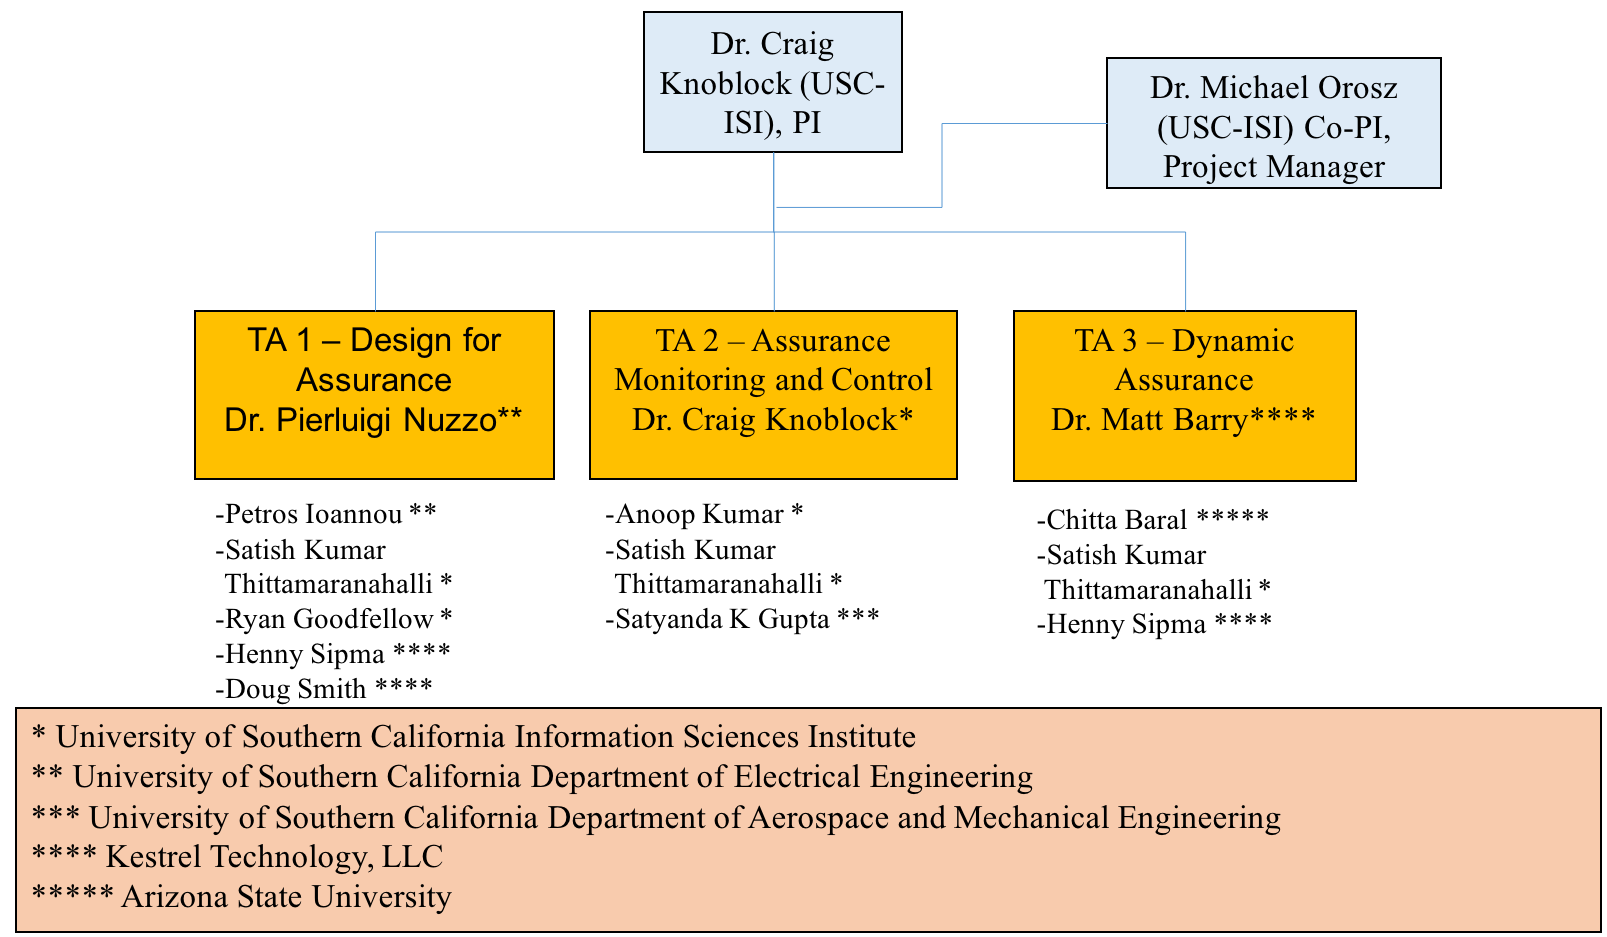
\includegraphics[width=6.0in]{./org-chart2.png}
\caption{\small Organization Chart}
\label{fig:org_chart}
\end{figure}

Coordination: To maximize collaboration and reduce risk to project failure from lack of communication and technical exchange, we plan to employ a wide variety of working styles and communication/coordination so that all can contribute.  At the core of our project will be regularly scheduled meetings bridging the diversely distributed team (Table~\ref{fig:Collaboration_Table}).  These meetings will address project status, identify challenges, implement risk mitigation strategies and participate in technology exchanges and system integration efforts (when appropriate)

\begin{table}[ht]
\caption{\small Project Meetings and Events}
  \centering
  {\footnotesize
\begin{tabular}{|m{3.15in}|m{3in}|} 
\hline
\textbf{Meeting} & \textbf{Frequency} 
\\\hline
Conference calls among investigators (discuss project status, address concerns and project risks) & Weekly
\\
\hline
Technical exchange and coordination meetings using Bluejeans or another videoconference technology & At least twice a month and more frequently as needed
  \\ 
\hline
Face-to-Face meetings (prior to P/I and demonstration meetings) & Every 3 to 6 months and more frequently (especially at the beginning of the project) as needed
 \\\cline{1-2}

\hline
\end{tabular}
}
\label{fig:Collaboration_Table}
\end{table}

\begin{table}[tbhp]
\caption{\small Key Project Team Member Responsibilities}
  \centering
  {\footnotesize
\begin{tabular}{| m{.75in} | m{3.9in}| m{1.5in}|} 
\hline
\textbf{Key Member} & \textbf{Responsibilities} & \textbf{Tasks} 
\\\hline
Dr.\ Craig Knoblock  & Principal Investigator responsible for project, leads TA 2 – Assurance Monitoring and Control.  Will lead the overall project and lead the TA2 team.  Served as the PI on many DARPA projects and has sucessfully led many large teams.    Effort on project:  25\% &
1.1.6, 1.2.2 1.2.3, 1.2.4, 1.3.4, 1.4.1, 
2.1.6, 2.2.2 2.2.3, 2.2.4, 2.3.4, 2.4.1, 
3.1.6, 3.2.2, 3.2.3, 3.2.4, 3.3.4, 3.4.1
\\
\hline
Dr.\ Michael Orosz & Co-Principal Investigator responsible managing the day-to-day operations of the project, assist technical teams as needed, coordinate with TA4 teams.    Has led many large complex multi-disciplined/multi-organizational projects in academic and industry environments.  Effort on project: 50\%
& 1.1.6, 2.1.6, 3.1.6, 1.4.1, 2.4.1, 3.4.1
  \\ 
\hline
Dr.\ Pierluigi Nuzzo 
& 
Co-Principal Investigator.  Leads the TA 1 - Design for Assurance team and conducts research on the formal methods for the design of the TA1 system.  Research experience on methodologies and tools for the design of cyber-physical systems; contracts, interfaces, and compositional methods for embedded system design; the application of automated formal methods and optimization theory to problems in embedded and cyber-physical systems.  Effort on project: 2 months/year (16.6\%)
& 
1.1.1, 2.1.1, 3.1.1 \\
\hline
Dr.\ Matthew Barry
& 
Key personnel.  Leads the TA 3 – Dynamic Assurance.   He will conduct the research on the dynamic assurance case language editors and parsers, the run-time system, and system integrations. Effort on project:  66\%
& 
1.3.2, 2.3.2, 3.3.2\\
\hline
Dr.\ Chitta Baral
& 
Key personnel responsible for learning assurance rules, supporting assurance rules with uncertainty and improving solver speed.  Expertise on ASP solvers, which will be used to reason about the assurance cases. Effort on project: 20\%
& 
1.3.1, 2.3.1, 3.3.1 \\
\hline
Dr.\ Doug Smith 
& 
Key personnel will support formal methods aspects of TA1, and lead the effort on abstract refinement. Expertise in field of automated correct-by-construction program generation.    Effort on project: 40\%
& 
1.1.5, 2.1.5, 3.1.5 \\
\hline
Dr.\ Henny Sipma
& 
Key personnel who will support the program verification tasks under TA1.  Will lead the effort on program verification.   Effort on project:  45\%
& 
1.1.5, 2.1.5, 3.1.5, 1.3.2, 2.3.2, 3.3.2 \\
\hline
Dr.\ Petros Ioannou
& 
Key personnel responsible providing and extending the assurance test bed, which will be available at the start of the project for autonomous vehicles.   Effort on project: 1 month/year (8.3\%)
& 
1.1.2, 2.1.2 (optional), 3.1.2 (optional)
\\
\hline
Dr.\ Satyandra Kumar Gupta
& 
Key Personnel providing autonomous command and control expertise to the TA-2 team.   Will lead the research on safety aware learning on TA2.   Past research on physics-aware decision making to facilitate automation.  Effort on project: 1 month/year (8.3\%)
& 
1.2.1, 2.2.1, 3.2.1 \\
\hline
Dr.\ Anoop Kumar 
& 
Key personnel providing support to the TA 2 project team.  Will lead the research on monitoring \& control and detecting distribution shifts.  Effort on project: 50\%
& 
1.2.1, 1.2.2, 1.2.3, 1.2.4, 2.2.1, 2.2.2, 2.2.3, 2.2.4, 3.2.1, 3.2.2, 3.2.3, 3.2.4\\
\hline
Dr.\ Satish Thittamaranahalli
& 
Key personnel developing scalable algorithms for TA1, TA2, and TA3 project teams.  Has extensive experience on scalable algorithm design, machine learning, and constraint reasoning.  Effort on project: 50\%
& 
1.2.1, 1.2.2, 1.2.3, 1.2.4, 2.2.1, 2.2.2, 2.2.3, 2.2.4, 3.2.1, 3.2.2, 3.2.3, 3.2.4, 1.1.4, 2.1.4, 3.1.4 \\
\hline
Dr.\ Ryan Goodfellow
& 
Key personnel providing support to the TA-1 project. Will lead the research on simulation-based testing.  Has extensive experience on simulation-based testing.  Effort on project:  30\%
& 
1.1.3, 2.1.3, 3.1.3 \\

\cline{1-2}

\hline
\end{tabular}
}
\label{fig:Table_Mgmt}
\end{table}



\newpage
\section{Personnel, Qualifications and Commitment}

{\bf Dr.\ Craig Knoblock}, the PI on this effort, is a Research Professor of both Computer Science and Spatial Sciences at the University of Southern California (USC) and Director of the Intelligent Systems Division at the USC Information Sciences Institute.   He received his Ph.D. from Carnegie Mellon University in computer science. 
%His research focuses on techniques for describing, acquiring, and exploiting the semantics of data.  
In previous projects he has worked on developing  scalable approaches to execution monitoring, accurate detection of sensor failures, and   automatic modeling and reconstruction of sensors.  He has published more than 300 journal articles, book chapters, and conference papers on these topics.  Dr. Knoblock is a Fellow of the Association for the Advancement of Artificial Intelligence (AAAI), a Distinguished Scientist of the Association of Computing Machinery (ACM), a Senior Member of IEEE, past President and Trustee of the International Joint Conference on Artificial Intelligence.
%and winner of the 2014 Robert S. Engelmore Award.  

{\bf Dr.\ Michael Orosz}, a Co-PI on this effort, is a Research Associate Professor of Civil and Environmental Engineering at the University of Southern California (USC) and Research Director of the Decision Systems Group at the USC Information Sciences Institute.  Dr. Orosz has over 30 years’ experience in commercial and government software development, basic and applied research, project management, academic research and has developed and deployed several commercially successful products.  His research interests are in machine learning and decision analytics as applied to intelligence analysis and autonomous command and control such as smart building controls.    Dr. Orosz has extensive experience in managing large complex multi-disciplined/multi-teamed research projects. %funded by DARPA, DHS, DoD, DoE, Industry, NASA, NRO, NSA and ONR.   
He received his Ph.D. in computer science from the University of California, Los Angeles.

{\bf Dr.\ Pierluigi Nuzzo}, a Co-PI on this project, is an Assistant Professor in the Department of Electrical Engineering at the University of Southern California. He received the Ph.D. in Electrical Engineering and Computer Sciences from the University of California at Berkeley. 
%in 2015, and the Laurea degree (MS) in electrical engineering (summa cum laude) from the University of Pisa, Italy, and the Sant'Anna School of Advanced Studies, Pisa, Italy.
%
%He has four years of research experience in analog and mixed signal circuit design as a researcher at IMEC, Leuven, Belgium, and over 10 years experience in design methodologies and tools for mixed-signal integrated circuits and cyber-physical systems, as a researcher at the University of Pisa, IMEC, UC Berkeley, and USC. 
His research interests
include: methodologies and tools for cyber-physical system and mixed-signal
system design; contracts, interfaces and compositional methods for embedded
system design; the application of formal methods and optimization theory to problems in embedded and cyber-physical systems and electronic design automation. 
%
Prof. Nuzzo received %First Place in the operational category and Best Overall
%Submission in the 2006 DAC/ISSCC Design Competition, 
a Marie Curie Fellowship
from the European Union in 2006, 
the University of California at Berkeley EECS
departmental fellowship in 2008, 
%the University of California at Berkeley Outstanding Graduate Student Instructor Award in 2013, 
the IBM Ph.D.
Fellowship in 2012 and 2014, 
%the Best Paper Award from the International Conference on Cyber-Physical Systems (ICCPS) in 2016, 
and the David J.~Sakrison Memorial Prize in 2016 for his doctoral research. 
%He is an author of 1 patent and over 60 publications.

{\bf Dr.\ Satyandra K. Gupta} is Smith International Professor in the Department of Aerospace and Mechanical Engineering at the University of Southern California. %Prior to joining the University of Southern California, he was a Professor in the Department of Mechanical Engineering and the Institute for Systems Research at the University of Maryland. He was the founding director of the Maryland Robotics Center and the Advanced Manufacturing Laboratory at the University of Maryland. 
He served as a program director for the National Robotics Initiative at the National Science Foundation from September 2012 to September 2014.  Dr. Gupta's interest is in the area of physics-aware decision making to facilitate automation. He has published more than 300 technical articles. He is a fellow of the American Society of Mechanical Engineers (ASME) and editor of ASME Journal of Computing and Information Science in Engineering. Dr. Gupta has received the Young Investigator Award from the Office of Naval Research in 2000, CAREER Award from the National Science Foundation in 2001, Presidential Early Career Award for Scientists and Engineers (PECASE) in 2001, Invention of the Year Award at the University of Maryland in 2007, Kos Ishii-Toshiba Award from ASME in 2011, and Excellence in Research Award from ASME in 2013.%, and Distinguished Alumnus Award from Indian Institute of Technology, Roorkee in 2014. %He has also received seven best paper awards at conferences.

{\bf Ryan Goodfellow} is a computer scientist at ISI working in combined cyber physical simulation and emulation platform development. His formal background is in simulation algorithms and modeling techniques using differential-algebraic equations (DAE). He has applied this knowledge in the CPS space by integrating DAE modeling languages and simulation engines with network testbeds to create comprehensive scientific experimentation platforms for cyber-physical systems. These experimentation platforms have been used in the power grid research space. %Ryan is a lead developer on the Deter network testbed, with a strong background in networked and distributed systems engineering. %He is also a combat veteran, serving as a non-commissioned officer and SIGINT team lead for a multi-functional intelligence team in Afghanistan.

{\bf Dr.\ Petros Ioannou} is a Professor in the Department of Electrical Engineering, Director of the Center for Advanced Transportation Technologies and Associate Director for Research for the DOT supported University Transportation Center at USC. He received his MS and PhD from the University of Illinois at Urbana Champaign in Mechanical and Electrical Engineering, respectively. His research interests are in robust adaptive control, vehicle dynamics and control, human factors and safety, automated vehicles, nonlinear systems and Intelligent transportation Systems.  He received the 2016 IEEE Transportation Technologies field award and the 2016 IEEE Control system society Transition to Practice Award. He is a Fellow of IEEE, IFAC and IET and author/coauthor of 8 books and over 400 papers.

{\bf Dr.\ Matthew Barry} will serve as lead for the TA3 tasks. %He will implement the dynamic assurance case language editors and parsers, the run-time system, and system integrations.  He will implement the assurance case arguments and the API for updating argument structure and content.  
Dr. Barry currently is CEO at Kestrel Technology LLC, and previously spent 20 years in NASA space mission operations at the Jet Propulsion Lab and Johnson Space Center.  At NASA Headquarters he led the introduction of dependability case requirements and plans for flight computing systems in upcoming manned space exploration missions, as well as the development of Agency-level software-related safety-critical control system requirements.  He recently served as a Principal Investigator on DHS/Cyber S\&T STAMP (Static Tool Analysis Modernization Program), DARPA CSFV (Crowd Sourced Formal Verification), three NASA Aeronautics R\&D projects, and the AFRL-sponsored Static Analysis of Numerical Algorithms project.  Dr. Barry earned BSME, MS, and PhD degrees in mechanical engineering, and an MBA degree, from Rice University.  

{\bf Dr.\ Henny Sipma} will support the program verification tasks under TA1.  %She is the key person behind the company's {\em KT Advance\/} and {\em KT Transferal\/} static analysis products, and the designer and programmer of the company's core {\em CodeHawk\/} abstract interpretation engine. 
Dr. Sipma currently is the CTO at Kestrel Technology LLC.  She has spent the past 10 years with Kestrel Technology as a static analysis expert; previously developed and taught static analysis techniques as senior research associate at Stanford University for eight years; and developed industrial process controls as an senior systems analyst at Shell.  She has been Principal Investigator or company lead on several recent R\&D projects for Federal agencies, including two projects under the IARPA STONESOUP (Securely Taking On New Executable Software of Uncertain Provenance) program; the DHS Cyber S\&T Gold Standard project; and the DARPA-sponsored STAC (Space-Time Analysis for Cybersecurity) and MUSE (Mining and Understanding Software Enclaves) programs.  Dr. Sipma earned 
%a BS degree in chemistry and an MS degree in chemical engineering at the University of Groningen in The Netherlands, and 
MS and PhD degrees in computer science from Stanford University.  

{\bf Dr.\ Douglas R.\ Smith} will support formal methods aspects of TA1, including the enforcement of safety properties and the generation of monitors.  He is President of Kestrel Technology LLC and Principal Scientist at Kestrel Institute.  He is a Fellow of the American Association of Artificial Intelligence (AAAI) and an ASE Fellow (Automated Software Engineering).  From 1986 to 2000, he taught an advanced graduate course on correct-by-construction software development at Stanford.  
%Dr. Smith has led the development of a series of software synthesis systems, including KIDS (Kestrel Interactive Development System), Specware, Designware, and Planware. 
%Applications domains have included a variety of complex high-performance planners and schedulers for the US Air Force.  He leads current projects on the generation of air mission plans and cyberoperations.  
Other recent projects focused on automated policy enforcement \cite{SmithD0703,SmithD08}, synthesis of secure network protocol codes, and the synthesis of high-performance constraint-solvers\cite{SmithD08c,SmithD13}.  Dr. Smith has over 30 years experience in the field of automated correct-by-construction program generation and has published over 100 papers. He has one patent.  He received the Ph.D. in Computer Science from Duke University% in 1979.  

{\bf Dr. Chitta Baral} is a Professor in the Department of Computer Science and Engineering at Arizona State University. He will support the TA3 efforts on Learning assurance rules, supporting assurance rules with uncertainty and improving solver speed. Dr. Baral has expertise in various aspects of autonomy and Artificial Intelligence. 
He wrote the first book on answer set programming (published by Cambridge University Press) the formal language behind our assurance rules. Some of his other works relevant to this proposal are: goal specification for autonomous systems, automatic construction of control rules for autonomous systems that satisfy given goals, combining machine learning with reasoning in various contexts, including image understanding. %He is the President of KR Inc. He is an associate editor of AIJ and has been an associate editor of JAIR.

{\bf Dr.\ Satish Kumar Thittamaranahalli (T. K. Satish Kumar)} leads the Collaboratory for Algorithmic Techniques and Artificial Intelligence (CATAI) at USC's Information Sciences Institute. He has published over 60 papers on numerous topics in Artificial Intelligence spanning such diverse areas as Constraint Reasoning, Planning and Scheduling, Probabilistic Reasoning, Robotics, Combinatorial Optimization, Approximation and Randomization, Heuristic Search, Model-Based Reasoning, Knowledge Representation and Spatio-Temporal Reasoning. %He %has served on the Program Committees of many international conferences in Artificial Intelligence
He and is a winner of the 2016 Best Robotics Paper Award and the 2005 Best Student Paper Award from the International Conference on Automated Planning and Scheduling. 
Dr. Kumar received his PhD in Computer Science from Stanford University. %In the past, he has also been a Visiting Student at the NASA Ames Research Center, a Postdoctoral Research Scholar at the University of California, Berkeley, a Research Scientist at the Institute for Human and Machine Cognition, a Visiting Assistant Professor at the University of West Florida, and a Senior Research and Development Scientist at Mission Critical Technologies.

\textbf{Dr.\ Anoop Kumar} is a senior computer scientist at USC ISI and has broad expertise in machine learning, statistical modeling, and software engineering.  Dr.\ Kumar is the technical lead on the DARPA RSPACE program and has played a vital role in developing a system that fuses air operations data from multiple sources, maintains world state, and issues warnings. Previously, he led the research and development of the BBN’s election forecasting system for the IARPA OSI program. %Dr.\ Kumar played a significant role in the DARPA DEFT program by developing a model to support integration of output from multiple NLP algorithms. He has contributed at the development to management levels on government research contracts and commercial projects. 
Dr.\ Kumar helped design and develop BBN's commercially available, hosted speech and medical transcription services offering. 

\begin{table}[!tbh]
\begin{footnotesize}
\vspace{-0.1in}

\begin{tabular}{lll}
\begin{tabular}[t]{|l|@{}c@{}|@{}c@{}|@{}c@{}|@{}c@{}|} \hline
Project & Status & \multicolumn{3}{ c| }{Hours} \\ \cline{3-5}
& & P1 & P2 & P3 \\ \hline



\multicolumn{5}{ |c| }{ \textbf{Craig Knoblock} } \\ \cline{1-5}
Safeguard & Pro & 770 & 641 & 641 \\ \cline{1-5}
ELICIT & Cur & 308 & 256 & 120 \\ \cline{1-5}
WTNIC & Cur & 11 & 0 & 0 \\ \cline{1-5}
EFFECT & Cur & 641 & 107 & 0 \\ \cline{1-5}
LinkedMaps & Cur & 203 & 25 & 0 \\ \cline{1-5}
PRINCESS & Cur & 608 & 96 & 0 \\ \cline{1-5}
SCHARP & Cur & 481 & 54 & 0 \\ \cline{1-5}
MINT & Pen & 650 & 534 & 285 \\ \cline{1-5}

\multicolumn{5}{ |c| }{ \textbf{Michael Orosz} } \\ \cline{1-5}
Safeguard & Pro & 1560 & 1300 & 1300  \\ \cline{1-5}
SMC/SY & Cur & 1803 & 0 & 0  \\ \cline{1-5}

\multicolumn{5}{ |c| }{ \textbf{Matthew Barry} } \\ \cline{1-5}
Safeguard & Pro & 2078 & 1690 & 1554 \\ \cline{1-5}
Starlite & Cur & 1840 & 1692 & 0 \\ \cline{1-5}



\multicolumn{5}{ |c| }{ \textbf{Anoop Kumar} } \\ \cline{1-5}
Safeguard & Pro & 1560 & 1300 & 1300 \\ \cline{1-5}

\end{tabular}
&
\begin{tabular}[t]{|l|@{}c@{}|@{}c@{}|@{}c@{}|@{}c@{}|} \hline
Project & Status & \multicolumn{3}{ c| }{Hours} \\ \cline{3-5}
& & P1 & P2 & P3 \\ \hline

\multicolumn{5}{ |c| }{ \textbf{Pierluigi Nuzzo} } \\ \cline{1-5}
Safeguard & Pro & 520 & 433 & 433  \\ \cline{1-5}
Mirage & Cur & 433 & 0 & 0  \\ \cline{1-5}

\multicolumn{5}{ |c| }{ \textbf{Satyandra Gupta} } \\ \cline{1-5}
Safeguard & Pro & 260 & 217 & 217 \\ \cline{1-5}
Human   & Cur & 22 & 0 & 0 \\ \cline{1-5}
Vehicles & Cur & 36 & 0 & 0 \\ \cline{1-5}
Robot & Cur & 116 & 0 & 0 \\ \cline{1-5}
Assembly & Cur & 33 & 0 & 0 \\ \cline{1-5}
Solar & Cur & 4 & 0 & 0 \\ \cline{1-5}

\multicolumn{5}{ |c| }{ \textbf{Petros Ioannou} } \\ \cline{1-5}
Safeguard & Pro & 260 & 217 & 217 \\ \cline{1-5}
CPS & Cur & 130 & 0 & 0 \\ \cline{1-5}

\multicolumn{5}{ |c| }{ \textbf{Ryan Goodfellow} } \\ \cline{1-5}
Safeguard & Pro & 936 & 780 & 780 \\ \cline{1-5}
STEAM & Cur & 416 & 0 & 0 \\ \cline{1-5}


\end{tabular}
&
\begin{tabular}[t]{|l|@{}c@{}|@{}c@{}|@{}c@{}|@{}c@{}|} \hline
Project & Status & \multicolumn{3}{ c| }{Hours} \\ \cline{3-5}
& & P1 & P2 & P3 \\ \hline

\multicolumn{5}{ |c| }{ \textbf{Chitta Baral} } \\ \cline{1-5}
Safeguard & Pro & 659 & 485 & 485 \\ \cline{1-5}
PostdocBP & Cur & 176 & 0 & 0 \\ \cline{1-5}
Languages & Pen & 528 & 264 & 264 \\ \cline{1-5}
CAREER & Pen & 88 & 44 & 44 \\ \cline{1-5}
CHS & Pen & 510 & 255 & 0 \\ \cline{1-5}

\multicolumn{5}{ |c| }{ \textbf{Doug Smith} } \\ \cline{1-5}
Safeguard & Pro & 1222 & 984 & 840 \\ \cline{1-5}
RSPACE & Cur & 342 & 0 & 0 \\ 
\cline{1-5}
PLANX & Cur & 154 & 0 & 0 \\ 
\cline{1-5}
HACCS & Pen & 923 & 769 & 769 \\ 
\cline{1-5}

\multicolumn{5}{ |c| }{ \textbf{Henny Sipma} } \\ \cline{1-5}
Safeguard & Pro & 1372 & 962 & 840 \\ \cline{1-5}
STAC & Cur & 797 & 0 & 0 \\ \cline{1-5}

\multicolumn{5}{ |c| }{ \textbf{Satish Thittamaranahalli} } \\ \cline{1-5}
Safeguard & Pro & 1560 & 1300 & 1300 \\ \cline{1-5}
MapF & Cur & 103 & 103 & 0 \\ \cline{1-5}

\end{tabular}
\end{tabular}

\end{footnotesize}
\caption{Individual commitments of key personnel}
\label{tab:Commitments}
\vspace{-0.2in}
\end{table}

\clearpage
\newpage
\section{Capabilities}


%\subsection{University of Southern California}
USC has strengths in number of areas that are closely related to the proposed work:
\begin{itemize}[itemsep=0pt,leftmargin=*]
\item Dr.\ Nuzzo 
%has over 10-year research experience in embedded system design, from mixed-signal chip design (analog-to-digital converters, frequency synthesizers, software-defined radio), to methodologies and tools for mixed-signal integrated circuits and Cyber-Physical Systems (CPSs), and the application of formal methods and optimization theory to problems in embedded and cyber-physical systems and electronic design automation.  
%His doctoral work 
has done extensive research on contracts and compositional methods for heterogeneous system design and design space exploration, with application to aircraft electric power systems and environmental control systems. His work has helped transition rigorous system design foundations, innovative design methodologies, and new systems engineering paradigms to industry (IBM, United Technologies). 
\item Dr.\ Satyandra K. Gupta has worked on autonomous surface vehicles, autonomous ground vehicles for operation on rugged terrains, and autonomous flapping wing aerial vehicles.   His group has developed a hierarchal decision making approach for realizing autonomous systems. 
%This approach combines task planning and assignment, deliberative trajectory planning, reactive collision avoidance behaviors, and trajectory tracking control layers. 
His group has also developed new methods for learning reactive behaviors in adversarial environments and COLREGS compliant trajectory planning. \item Dr.\ Knoblock has developed methods that learn the relationships between sensors to both identify failures and changes in sensor and reconstruct those sensors, providing estimates of the accuracy of the reconstructed sensors.  
\item Ryan Goodfellow has extensive experience in simulation based testing through high-fidelity CPS testbed environment development and operation, using the Deter network testbed as the core which has supported several large scale government projects from a variety of agencies and thousands of users. %we have developed sophisticated CPS experiments under programs such as NFS RIPS, NIST SmartCities and the DHS Cybersecurity showcase.
\item Dr.\ Ioannou %helped  design and implement adaptive cruise control systems in collaboration with Ford Motor Company, which was commercialized four years before any other company. He 
worked on several DOT funded projects on automated vehicles and intelligent highway systems where he demonstrated his vehicle control designs for safety and performance on actual automated vehicles in test trucks and I-15 highway.
\item Drs.\ Knoblock, Kumar, and Thittamaranahalli have developed highly scalable approaches for monitoring message traffic to identify potential problems and issue warnings and alerts. 
\item Dr. Thittamaranahalli has developed state-of-the-art methods for efficiently solving large-scale search and optimization problems. %These techniques will be applicable in TA2 for safety-aware learning and planning, in TA2 for assurance monitoring and control, and in TA3 for dynamic assessment of assurance cases.

\end{itemize}
%\subsection{Kestrel Technology LLC}

Kestrel Technology's strength is in program analysis, specifically static analysis of both source and binary targets.  The company performs applied R\&D and product development for a variety of static analysis applications  pivoting primarily on the abstract interpretation technique.  The company recently initiated development of program analysis applications using logical equivalence techniques. As a provider of verification evidence in the form of mathematical proofs, the company also has expertise in the design and development of assurance case arguments for high-integrity systems using such evidence. %The company is engaged in a partnership with Wind River Systems to develop program analysis tools for its embedded system developers.  Many of Wind River's customers must develop their products under safety and certification standards, including those using safety cases.  

   

%\subsection{Arizona State University}
Chitta Baral at Arizona State University has developed various software to learn assurance rules and various ASP solvers, which he has made available as open-source.

Most of the software carried forward for implementation or derivation is open source.  The single exception is Kestrel Technology's {\it KT Advance\/} static analysis tool (TA1), in particular the abstract interpretation engine therein, which is company proprietary and is US EAR export-controlled.   
%Owing to mixed funding for the development of that technology 
We will continue to provide the Federal government a restricted use license for that particular item.

There are no specialized facilities, data, or GFE required for this effort. 

\include{sow}
\include{milestones}

% \section{Level of Effort by Task \textcolor{red}{[Mike/Lisa - 1 pages]}}

% \textcolor{blue}{
% \begin{itemize}
% \item Will be a separate spreadsheet
% \item
% \end{itemize}
% }

\include{appendix_a}

%\section{Appendix B \textcolor{red}{[No Page Count]}}

\section{References}
\bibliographystyle{acm} 
\bibliography{TA3/ta3,TA2/ta2,TA1/ta1}
\end{document}
%%\documentclass[a4paper]{article}
%\documentclass[12pt]{article}
\documentclass[12pt]{dod-blank}

%% Language and font encodings
\usepackage[english]{babel}
\usepackage[utf8x]{inputenc}
\usepackage[T1]{fontenc}

%% Sets page size and margins
%%\usepackage[a4paper,top=3cm,bottom=2cm,left=3cm,right=3cm,marginparwidth=1.75cm]{geometry}
%\usepackage[top=1in, bottom=1in, left=1in, right=1in]{geometry}



%% Useful packages
\usepackage{amsmath}
\usepackage{graphicx}
  \graphicspath{{.}{./image/}}
  \DeclareGraphicsExtensions{.png,.jpg} 
\usepackage[colorinlistoftodos]{todonotes}
\usepackage[colorlinks=true, allcolors=blue]{hyperref}
\usepackage{tabularx}
\usepackage{multirow}
\usepackage{tabulary}
\usepackage{float}
\usepackage{wrapfig}
\usepackage[export]{adjustbox}
\usepackage{comment}
\usepackage{tabularx}
\usepackage{multirow}
\usepackage{tabulary}
\usepackage{enumitem}

\usepackage{listings}
\usepackage{color}
\usepackage{array}
\usepackage{subcaption}
\usepackage{xcolor}




\renewcommand{\textfraction}{0}
\renewcommand{\topfraction}{1.0}
\renewcommand{\bottomfraction}{1.0}

\usepackage{longtable}
%% macros
\newif\iffinal
\finaltrue
\iffinal
  
    \newcommand\baareq[1]{}
    \newcommand\baades[1]{}
 
 
\else
    \definecolor{darkgreen}{rgb}{0,0.4,0}
    \definecolor{darkcyan}{rgb}{0,0.4,0.4}
    \definecolor{darkblue}{rgb}{0,0,0.5}
    
    \newcommand\baareq[1]{{\color{darkcyan}[\textbf{Requirement:} #1]}}
    \newcommand\baades[1]{{\color{darkcyan}[\textbf{Description:} #1]}}
 
\fi




\def\naive{na\"{\i}ve}



\lstset{ 
  backgroundcolor=\color{white},   % choose the background color; you must add \usepackage{color} or \usepackage{xcolor}
  basicstyle=\footnotesize\ttfamily,            % the size of the fonts that are used for the code
  breakatwhitespace=false,         % sets if automatic breaks should only happen at whitespace
  breaklines=true,                 % sets automatic line breaking
  captionpos=b,                    % sets the caption-position to bottom
  commentstyle=\color{mygreen},    % comment style
  % deletekeywords={...},            % if you want to delete keywords from the given language
  escapeinside={\%*}{*)},          % if you want to add LaTeX within your code
  extendedchars=true,              % lets you use non-ASCII characters; for 8-bits encodings only, does not work with UTF-8
  frame=single,	                   % adds a frame around the code
  keepspaces=false,                 % keeps spaces in text, useful for keeping indentation of code (possibly needs columns=flexible)
  keywordstyle=\color{blue}\bfseries\underbar,       % keyword style
  language=Prolog,                 % the language of the code
  % morekeywords={if,and},        % if you want to add more keywords to the set
  numbers=none,                    % where to put the line-numbers; possible values are (none, left, right)
  numbersep=5pt,                   % how far the line-numbers are from the code
  numberstyle=\tiny\color{mygray}, % the style that is used for the line-numbers
  rulecolor=\color{black},         % if not set, the frame-color may be changed on line-breaks within not-black text
  showspaces=false,                % show spaces everywhere adding particular underscores; it overrides 'showstringspaces'
  showstringspaces=false,          % underline spaces within strings only
  showtabs=false,                  % show tabs within strings adding particular underscores
  stepnumber=2,                    % the step between two line-numbers. If it's 1, each line will be numbered
  stringstyle=\color{mymauve},     % string literal style
  tabsize=2,	                   % sets default tabsize to 2 spaces
  title=\lstname                   % show the filename of files included with \lstinputlisting; also try caption instead of title
}

% apply trick for additional keywords for our AC DSL
\lstset{
	emph={for, if, and, or},
    emphstyle={\color{blue}\bfseries\underbar}
}




\title{DARPA Assured Autonomy}
\author{Technical Volume- \textcolor{red}{Thirty-Eight (38) pages max}}

\begin{document}
\pagenumbering{roman}
\include{cover}

\newpage
\section{Table of Contents}
\tableofcontents

\newpage
\pagenumbering{arabic}
\section{Executive Summary}
As we rapidly move into a world where machine learning plays a central role in realizing autonomous systems, it is becoming increasingly important to develop techniques that assure that these systems will operate safely and perform as expected. Current approaches are limited to providing assurance for systems with limited or no  learning capabilities. In this context, DARPA's Assured Autonomy BAA seeks to \emph{develop rigorous design and analysis technologies for continual assurance of learning-enabled autonomous systems}. USC in collaboration with Kestrel Technology and ASU is pleased to submit a comprehensive TA1, TA2, and TA3 proposal entitled \emph{``Assured Autonomy for Learning Enabled Vehicles (Safeguard).''} We plan to provide an end-to-end solution to support autonomous systems with learning-enabled components, ranging from design technologies for assurance, to assurance monitoring and control techniques, to representation and online evaluation of assurance cases. We have assembled a strong team of experts that cover the range of technologies that are required to create such an end-to-end system. If successful, the project will provide the technologies for building the next-generation of learning-enabled autonomous systems.  The entire project will take four years and cost \textcolor{red}{\$??}, with an initial version completed at the end of Phase I and successive versions with additional capabilities and improved scalability at the end of Phase II and Phase III.  

In the remainder of this section, we first introduce an  unmanned surface vehicle scenario that will be used throughout the proposal to describe the approach.  Next, we describe our approach to design, monitoring, and dynamic assurance. Finally, we introduce the team involved in the project. 

\textbf{Motivating Scenario.} Consider an autonomous unmanned surface vehicle (USV) guarding a valuable asset in the ocean when an unknown vehicle  approaches the security perimeter, under challenging weather conditions. In this scenario, the USV is required to approach the intruding vehicle, issue a warning signal, and escort it to a safe distance from the controlled area. However, as the USV has no a priori knowledge of its external environment behaviors (e.g., water depth, waves, wind, current, visibility), pre-computing a feasible trajectory, let alone optimal, becomes a non-trivial problem. For trajectory planning, the USV must continuously perform the following tasks:
\begin{itemize}[itemsep=0pt,leftmargin=*]
 \item Sense the current state of the surrounding environment (e.g., water depth, waves, wind, current, visibility) and estimate its own maneuverability constraints (e.g., braking distance, available acceleration, maximum velocity, turning radius, turning rate, safety distance) based on the state of the environment;      
\item Sense the static obstacles in the sensor range and generate a traversability map;
\item Sense the moving obstacles and classify them;   
\item Predict future trajectories of moving obstacles; 
\item Determine if any of the COLREGS \cite{commandant1999international} rules will be in effect with respect to one or more of the nearby vessels and identify the vessels with the right of way.    
\end{itemize}
The above information will be used by the trajectory planner to compute an initial trajectory, which will be continuously refined as the USV gathers additional information.
% It is not possible for the USV to be tested in every possible environment. 
The USV will use learning enabled components to take  decisions as it encounters new situations, such as  
\begin{itemize}[itemsep=0pt,leftmargin=*]
\item Classifiers to identify moving obstacles based on physical appearance and motion signatures,
\item Algorithms to estimate the sensor capabilities in adverse weather conditions,   
\item Algorithms to accurately estimate uncertainty in the environment, 
\item Classifiers to generate traversability maps,
\item Prediction of external vessel behaviors based on motion histories, 
\item Reinforcement learning  to ensure COLREGS compliance of maneuvers,  
\item Algorithms to learning pursuit behaviors.  
\end{itemize}
Learning enabled components will interact with each other in complex ways, where a misclassification error in one component may eventually compromise the entire mission.   
% We will need to make sure that each learning enabled components has a run-time monitor that will ensure that the assumptions made by the learning-enabled component remain valid and prevent erroneous learning. 
% For example, if the vehicle is exhibiting significant error in trajectory tracking, then simply downgrading the trajectory tracking error value may not be a good option.  The failure of prediction of trajectory tracking error might be due to the presence of a significant wake caused by a nearby vessel. The presence of the nearby vessel can be used to explain the degradation in trajectory tracking performance. As the vessel moves away, we can expect the trajectory tracking performance to return to the predicted level.  
While exhaustive validation of learning-enabled cyber-physical systems (LE-CPSs) is a prohibitive task~\cite{Kalra16},
their complexity, heterogeneity, and highly dynamic nature
make it challenging to even leverage existing model-based development techniques to effectively assess system correctness 
% dependability, 
at design time or enforce it at runtime.

\textbf{Design for Assurance.} Safeguard uses a platform-based design approach~\cite{Nuzzo15b} to organize the design process for a LE-CPS and to build assurance cases. Composite models are developed at several levels of abstraction,
from top-level system requirements and safety constraints down to the
implementation level.  Intermediate levels add detail to the levels
above.  The different levels are connected by refinement mappings that
allow properties established at one level to be preserved at the next
level (see Figures~\ref{fig:methodology} and~\ref{fig:assurance}).

Contracts are used to formally specify components and composite models
in terms of (1) Assumptions -- the assumed behaviors of the
environment and the behaviors of other components, and (2) Guarantees
-- the behavior properties that a model guarantees if it operates in a
context that satisfies its assumptions.  A calculus of contracts
allows horizontal composition of contracts to generate contracts for
composite models.  Vertical contracts are used to specify the mapping
or refinement relation between models at different levels of
abstraction.  The system design process starts with a high-level
contract that expresses overall system assumptions and requirements.
Subsequent levels express models with increasing detail until the
lowest level expresses the system in terms of hardware components and
their software controllers.

The assurance case for a CPS arises from the horizontal and vertical
structure of the design in several ways.  The components used within a
particular level are either (1) synthesized using
correct-by-construction design tools together with proofs, (2) derived
statically or dynamically using safety-aware machine-learning
techniques, (3) written manually and verified by analysis tools, or
(4) written manually and validated by extensive testing.  The
assurance case for the whole reflects its compositional structure.  We
anticipate that well-specified contracts together with the calculus of
contracts will eliminate well-known problems with unexpected emergent
behaviors in CPS systems.

The assurance case for the lowest-layer design arises from both the
intra-level assurance and from properties and their proofs that are
preserved under the refinement mapping from the top-level
requirements.  The refinement mappings between model layers will be
constructed using a variety of techniques.  A contract at an abstract
level can be mapped to a component or refined contract by (1)
retrieval of pre-verified components from a platform library, (2)
synthesis using correct-by-construction design and optimization tools,
or (3) manual coding to satisfy a contract.  The mapping of a
composite model will be composed from the mappings of its constituent
components or contracts.  When a composite model cannot be mapped
compositionally to the next level, it will be generated using
correct-by-construction design and optimization tools.

\textbf{Assurance Monitoring and Control.}
We provide an integrated framework for safety-aware learning, assurance monitoring and control, detecting distribution shifts. Three major components offer an efficient TA2 architecture as well as interfaces with TA1 and TA3, that is, (a) safety-aware learning and planning, (b) assurance monitors for guarding architectural and safety constraints; and (c) distribution shift detection.

We will develop a new learning-enabled online decision-making framework that allows opportunistically composing a sequence of actions (maneuvers) to reduce uncertainty in the system capability model without suspending the progress toward the mission goals or compromising safety. Each candidate action is evaluated based on three criteria: (1) the risk of violating a safety constraint using the current uncertainties in the parameter estimates; (2) its relevance to the mission goals; (3)  its expected information gain, i.e., reduction in uncertainty, with respect to the parameter estimates. These evaluations are combined to produce a cumulative mission utility value for each action that drives our learning-enabled decision-making framework. The problem of generating and evaluating sequences of actions can be posed in several way. For example, it can be solved using a branch-and-bound search method like Anytime A*, or formulated with the finite-horizon Markov Decision Process (MDP) framework. We will develop new scalable search strategies to solve this problem efficiently, by potentially evaluating a recent method developed at USC, called FastMap, that can significantly improve the execution time. 

We will develop monitors for architectural and safety constraints. 
% While these constraints can be checked over and over again as sensor information flow in, this naive strategy accounts for a lot of computational overhead. 
To achieve scalability and decrease the overhead, we propose the application of a technique that we currently use in DARPA's RSPACE program, which leverages a physical model of the vehicles dynamics and its interactions with the environment to efficiently determine the readout frequency. We propose two  extensions of this basic idea. First, we will use the theory of Variable Elimination to prioritize which variables to monitor, e.g., controllable, versus uncontrollable, adversarially controlled, or unobservable variables. Second, we invoke the dynamic assessment of assurance cases only when needed. This  decreases the number of times dynamic assessment of assurance cases is initiated as well as the communication bandwidth between the TA2 and TA3 components.

Finally, we will identify a distribution shift by combining statistical and machine learning techniques to differentiate between environmental and sensor changes. We will exploit a categorization of the shifts based on their cause and duration as well as extend our earlier work on detecting and mitigating sensor failures for all types of monitored variables.  

\textbf{Dynamic Assurance:} The Safeguard {\em design for assurance\/} activity takes a systems-theoretic stance toward safety.  Consequently, it presumes that safety is an emergent property of the system, and that hazards can present themselves through unintended interactions and performance violations in addition to causal events such as component failures.  Our design approach includes consideration of intent as well as hazard analysis and mitigation.  The artifacts from these activities populate contracts and assumptions for the dynamic assurance case.  
We thus build safety into the product by working at a systems-level viewpoint, using lexicon and design patterns familiar to both hardware and software engineers; safety is an emergent property of the system, not an afterthought.  
As system behavior evolves during runtime owing to learning, threats, degradation, or some other factor, the dynamic assurance case identifies whether the safety constraints continue to be satisfied.  If not, it provides notifications or issues recovery instructions directly from a lookup table.

Our implementation of the dynamic assurance case employs a declarative knowledge base inference engine and a domain-specific language tailored to our approach.  We have used them successfully for assurance case tool sets and arguments, and will extend them to reason about uncertainty and learning.  Our approach to achieve scalability is to specialize solvers toward modularity and to take advantage of domain knowledge.  Specifically, we will develop answer set programming techniques for context-dependent learning for reasoning about the learning-enabled components as well as learning assurance rules.  We will develop new formalisms for uncertainty to include causality, using weights for computing probabilities, and probabilistic non-monotonicity.  To achieve scaling objectives we will implement specializations using modularity, weighted CSPs, and message passing. 

% The system safety constraints revealed from that design become the key elements of our dynamic assurance case.  Our verification tools ensure the constraints are relevant, identifiable, and their implementation and effect observable.  

\textbf{Team.} We have assembled a team that is exceptionally well-qualified to build the proposed Safeguard system.  The team will be led by Dr.\ Craig Knoblock, the Principal Investigator for the effort, who currently leads the Intelligent Systems Division at the Information Sciences Institute.  He has led many large DARPA and IARPA projects over the years and has a strong track record in conducting leading edge research and then transitioning the technology to commercial use.  He will be supported by Dr.\ Michael Orosz as the Project Manager, who also has  experience in managing large research projects and on autonomous systems.  The TA1 team will be led by Dr.\ Pierluigi Nuzzo, who is an expert in embedded system design methodologies and the  application of formal methods to cyber-physical systems.  The TA1 team also includes Dr.\ Doug Smith, who has spent many years working on scalable correct-by-construction techniques and Dr.\ Henny Sipma, who has significant experience in applying program verification methods to real-world problems.  The TA1 team also includes Ryan Goodfellow, who has done a large amount of work on simulation-based testing.  The TA2 team will be led by Dr.\ Knoblock who has worked on topics related to both monitoring and detecting distribution changes.  He will be supported by Dr.\ Satyandra Gupta, who is an expert on autonomous surface vehicles as well as on safety-aware learning. He will also be supported by Drs.\ Anoop Kumar and Satish Thittamaranahalli, who have also previously worked on efficient methods for execution monitoring.  The TA3 team will be lead by Dr.\ Matthew Barry, who has experience in creating the technologies for assurance cases.  He will be supported by Dr.\ Chitta Baral, who is an expert on ASP solvers and by Dr.\ Thittamaranahalli who is an expert on SAT solvers, both of which will be applied to provide scalable assurance case reasoning.  Finally, Dr.\ Petros Ioannou, who is an expert on control systems for autonomous vehicles will provide an autonomous vehicle platform, which will form the focus of our work until the TA4 teams provide additional vehicle platforms for development.  

\newpage
\section{Innovative Claims and Deliverables}

In this project we will develop and build an end-to-end system for assured autonomy.  This section describes the key innovations by technical area and then the overall deliverables of the project.

\paragraph{Design for Assurance}

\begin{itemize}[itemsep=0pt,leftmargin=*]
\item We address the LE-CPS design challenges via a holistic approach that can contextually generate design artifacts and assurance cases. We develop a compositional, contract-based modeling framework, methods, and tools to support the design process from system-level requirement capture,  formalization, and analysis, to the generation, testing, and continual monitoring of software and hardware artifacts in feedback loop with a physical process.

\item We develop compositional abstractions and interfaces (vertical contracts) that can  bridge heterogeneous formalisms and heterogeneous decomposition architectures to make system analysis and synthesis tractable, consistently combine different verification and synthesis methods at design time, and provide seamless support for dynamic assurance at run time. %We aim to quantitatively capture the confidence in the satisfaction of requirements under uncertain or unknown conditions, and resilience properties of  systems at different abstraction levels, to enable trade-off evaluation between resilience, performance, and cost.

\item We develop a unifying framework and efficient algorithms to reason about the combination of discrete and continuous dynamics and constraints in the presence of uncertainties in LE-CPS using a satisfiability modulo convex approach~\cite{Shoukry2017} for contract-based system verification and scalable trajectory planning.  

\item We provide an environment for high-fidelity CPS testing, in which production-ready software, e.g.,  safety-critical learning and control, may be deployed and tested 
% by extending the Cypress testbed environment \cite{Goodfellow2015Cypress:Systems} 
with time dilation facilities, so that it synchronizes with a physical simulation that is not necessarily running in real time, while still having the perception of real time.

\item We 
% These facilities allow a cyber system to be  
propose an approach for unanticipated behavior space identification and test coverage maximization which leverages results from the theory of differential algebraic equation (DAE)~\cite{Berger2013ControllabilitySurvey,Ilchmann2005ATheory,BergerOnSystems,Lamour2013} 
to prune the behavior search space and identify smaller regions of interest for efficient simulation-based testing. 
% We then compute the intersection of these two behavior spaces and restrict our simulation based testing search space to this subspace.
\end{itemize}

\paragraph{Assurance Monitoring and Control}

\begin{itemize}[itemsep=0pt,leftmargin=*]
\item 
%We integrate safety-aware learning into the overall decision making problem. The goal is to maximize mission utility without violating the safety constraints. 
Our safety-aware learning framework enables the system to opportunistically select and execute actions to assist the learning-enabled component in reducing model uncertainty without compromising safety or deviating from the mission goals. The value of uncertainty reduction is explicitly incorporated in the optimization process for selecting the best action.  
\item For safety-aware learning, we propose the idea of preprocessing the search space of the problem domain before queries and observations come in. With such a linear-time preprocessing phase, the performance of search and optimization algorithms can be significantly boosted. For example, in regular A* search, the intensional or extensional search space can be preprocessed in near-linear time to yield an embedding of each state as a point in Euclidean space~\cite{cujakk}. Then, when the query comes in, A* search can make use of these Euclidean distances as heuristic distances between two states to yield order-of-magnitude speedups. 
%In Anytime A* for safety-aware learning and planning, this leads to a significantly better quality of actions chosen within a time limit, and in the MDP framework, the same ideas can be used to improve the convergence of Bellman updates for safety-aware Reinforcement Learning.
\item As massive amounts of sensor information flow in, it is imperative for us to efficiently process this information for monitoring architectural and safety constraints. Building on our past work on similar tasks, we propose novel technologies for efficiently monitoring constraints. These algorithms can yield an exponential reduction in the amount of sensor data that needs to be processed. Doing this also reduces the message complexities between the various modules. %We also propose to use the theory of Variable Elimination (VE) to monitor constraints with uncontrollable, adversarially controlled, and/or unobservable variables. VE yields a substrate constraint to monitor that characterizes a dominant strategy of the controllable variables over the uncontrollable, adversarially controlled, and/or unobservable variables.
\item We will develop techniques to identify  distributional shifts and determine the underlying cause (e.g., change in environment, sensor failure,   etc.), as well as strategies for handling the various distributional shifts.   Notably, we propose to build on our past work and use compact representations to exploit historical data to identify distributional shifts.
\end{itemize}

\paragraph{Dynamic Assurance}

\begin{itemize}[itemsep=0pt,leftmargin=*]

\item We demonstrate the integration of dynamic assurance for safety-critical learning-enabled dynamic systems in which evolutionary behaviors are expected and tolerated as a property of the functionality.   The impact will be consequential contributions safety-critical dynamic systems in which evolutionary behaviors are expected and tolerated as portion of the functionality.   
\item We implement dynamic assurance by combining features of system safety, formal methods, logic programming, uncertain reasoning, and domain-specific languages.  We populate assurance case arguments at several levels of modeling and implementation abstraction, using the analysis results to produce design-time evidence supporting assurance claims.  
%We provide automated reasoning about the assurance case itself to produce verification, consistency, and completeness results for the argument.  Dynamic assurance results then yield trusted explanations of whether safety constraints and assumptions and other contracts still hold during the collection of runtime evidence from monitors. 
\item We develop and demonstrate ASP formalisms crucial to applications in dynamic assurance. We demonstrate the suitability of the technology especially for assurance case arguments owing to the improved legibility, consistency and completeness checks, handling of uncertain and default reasoning, and scalability.  
%We will produce modularized solvers for enhanced performance based on recent algorithmic developments in exploiting structure, kernelization, and message passing. We provide a formalism to enable learning of assurance rules. 
We provide a novel approach to handling uncertainty that provides the ability to do causal and counter-factual reasoning as well as probabilistic non-monotonicity.  Overcoming limitations of traditional inductive logic techniques, we develop a novel iterative and incremental approach based on context dependent learning. 
\end{itemize}

\paragraph{Deliverables}
During the course of this project, we will build and deliver a fully-operational system that covers all three of the technical areas.  The detailed capabilities of this system are described in the individual technical sections.  The resulting system will be available as open source under a permissive license, which will allow other organizations to use the work, extend it in new directions, and even commercialize the software.  Kestrel Technology has significant experience in this space and has built and applied these types of technologies to a variety of real world tasks.  Kestrel is ideally suited to pursue commercial uses of this technology and the permissive license will facilitate exploring these opportunities since there will be no need to negotiate intellectual property rights.  

\newpage
\section{Technical Plan}
\input{./TA1/main}
\input{./TA2/main}
\input{./TA3/main}
\clearpage
\newpage


\section{Management Plan}


The Principal Investigator for this effort is Dr. Craig Knoblock who is responsible for all aspects of the effort, will coordinate the parallel team efforts, and will ensure high levels of performance from individual team members.  The Co-P/I, Dr. Michael Orosz, will provide project management and will assist all performers in the execution of the project.    The project team is divided into three working groups (Figure~\ref{fig:org_chart}) corresponding to Technical Areas 1-3, however, members of each team contribute across all project activities.   Table~\ref{fig:Table_Mgmt} defines the major contributions of each project team member to the project tasks.

\begin{figure}[tbhp]
%\vspace{-25pt}
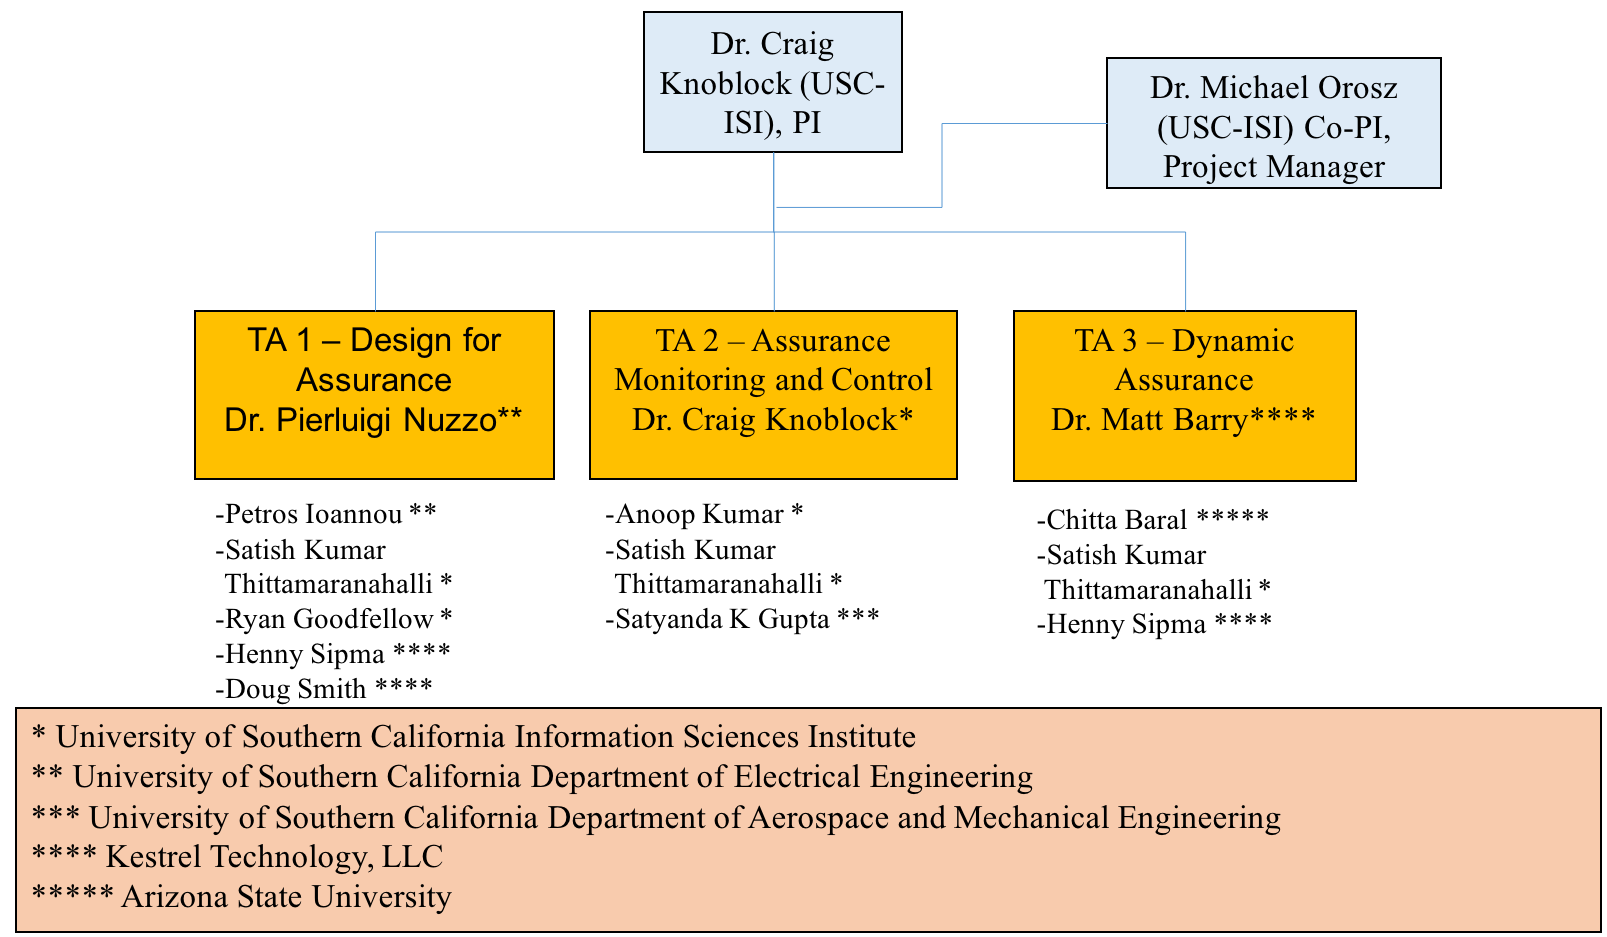
\includegraphics[width=6.0in]{./org-chart2.png}
\caption{\small Organization Chart}
\label{fig:org_chart}
\end{figure}

Coordination: To maximize collaboration and reduce risk to project failure from lack of communication and technical exchange, we plan to employ a wide variety of working styles and communication/coordination so that all can contribute.  At the core of our project will be regularly scheduled meetings bridging the diversely distributed team (Table~\ref{fig:Collaboration_Table}).  These meetings will address project status, identify challenges, implement risk mitigation strategies and participate in technology exchanges and system integration efforts (when appropriate)

\begin{table}[ht]
\caption{\small Project Meetings and Events}
  \centering
  {\footnotesize
\begin{tabular}{|m{3.15in}|m{3in}|} 
\hline
\textbf{Meeting} & \textbf{Frequency} 
\\\hline
Conference calls among investigators (discuss project status, address concerns and project risks) & Weekly
\\
\hline
Technical exchange and coordination meetings using Bluejeans or another videoconference technology & At least twice a month and more frequently as needed
  \\ 
\hline
Face-to-Face meetings (prior to P/I and demonstration meetings) & Every 3 to 6 months and more frequently (especially at the beginning of the project) as needed
 \\\cline{1-2}

\hline
\end{tabular}
}
\label{fig:Collaboration_Table}
\end{table}

\begin{table}[tbhp]
\caption{\small Key Project Team Member Responsibilities}
  \centering
  {\footnotesize
\begin{tabular}{| m{.75in} | m{3.9in}| m{1.5in}|} 
\hline
\textbf{Key Member} & \textbf{Responsibilities} & \textbf{Tasks} 
\\\hline
Dr.\ Craig Knoblock  & Principal Investigator responsible for project, leads TA 2 – Assurance Monitoring and Control.  Will lead the overall project and lead the TA2 team.  Served as the PI on many DARPA projects and has sucessfully led many large teams.    Effort on project:  25\% &
1.1.6, 1.2.2 1.2.3, 1.2.4, 1.3.4, 1.4.1, 
2.1.6, 2.2.2 2.2.3, 2.2.4, 2.3.4, 2.4.1, 
3.1.6, 3.2.2, 3.2.3, 3.2.4, 3.3.4, 3.4.1
\\
\hline
Dr.\ Michael Orosz & Co-Principal Investigator responsible managing the day-to-day operations of the project, assist technical teams as needed, coordinate with TA4 teams.    Has led many large complex multi-disciplined/multi-organizational projects in academic and industry environments.  Effort on project: 50\%
& 1.1.6, 2.1.6, 3.1.6, 1.4.1, 2.4.1, 3.4.1
  \\ 
\hline
Dr.\ Pierluigi Nuzzo 
& 
Co-Principal Investigator.  Leads the TA 1 - Design for Assurance team and conducts research on the formal methods for the design of the TA1 system.  Research experience on methodologies and tools for the design of cyber-physical systems; contracts, interfaces, and compositional methods for embedded system design; the application of automated formal methods and optimization theory to problems in embedded and cyber-physical systems.  Effort on project: 2 months/year (16.6\%)
& 
1.1.1, 2.1.1, 3.1.1 \\
\hline
Dr.\ Matthew Barry
& 
Key personnel.  Leads the TA 3 – Dynamic Assurance.   He will conduct the research on the dynamic assurance case language editors and parsers, the run-time system, and system integrations. Effort on project:  66\%
& 
1.3.2, 2.3.2, 3.3.2\\
\hline
Dr.\ Chitta Baral
& 
Key personnel responsible for learning assurance rules, supporting assurance rules with uncertainty and improving solver speed.  Expertise on ASP solvers, which will be used to reason about the assurance cases. Effort on project: 20\%
& 
1.3.1, 2.3.1, 3.3.1 \\
\hline
Dr.\ Doug Smith 
& 
Key personnel will support formal methods aspects of TA1, and lead the effort on abstract refinement. Expertise in field of automated correct-by-construction program generation.    Effort on project: 40\%
& 
1.1.5, 2.1.5, 3.1.5 \\
\hline
Dr.\ Henny Sipma
& 
Key personnel who will support the program verification tasks under TA1.  Will lead the effort on program verification.   Effort on project:  45\%
& 
1.1.5, 2.1.5, 3.1.5, 1.3.2, 2.3.2, 3.3.2 \\
\hline
Dr.\ Petros Ioannou
& 
Key personnel responsible providing and extending the assurance test bed, which will be available at the start of the project for autonomous vehicles.   Effort on project: 1 month/year (8.3\%)
& 
1.1.2, 2.1.2 (optional), 3.1.2 (optional)
\\
\hline
Dr.\ Satyandra Kumar Gupta
& 
Key Personnel providing autonomous command and control expertise to the TA-2 team.   Will lead the research on safety aware learning on TA2.   Past research on physics-aware decision making to facilitate automation.  Effort on project: 1 month/year (8.3\%)
& 
1.2.1, 2.2.1, 3.2.1 \\
\hline
Dr.\ Anoop Kumar 
& 
Key personnel providing support to the TA 2 project team.  Will lead the research on monitoring \& control and detecting distribution shifts.  Effort on project: 50\%
& 
1.2.1, 1.2.2, 1.2.3, 1.2.4, 2.2.1, 2.2.2, 2.2.3, 2.2.4, 3.2.1, 3.2.2, 3.2.3, 3.2.4\\
\hline
Dr.\ Satish Thittamaranahalli
& 
Key personnel developing scalable algorithms for TA1, TA2, and TA3 project teams.  Has extensive experience on scalable algorithm design, machine learning, and constraint reasoning.  Effort on project: 50\%
& 
1.2.1, 1.2.2, 1.2.3, 1.2.4, 2.2.1, 2.2.2, 2.2.3, 2.2.4, 3.2.1, 3.2.2, 3.2.3, 3.2.4, 1.1.4, 2.1.4, 3.1.4 \\
\hline
Dr.\ Ryan Goodfellow
& 
Key personnel providing support to the TA-1 project. Will lead the research on simulation-based testing.  Has extensive experience on simulation-based testing.  Effort on project:  30\%
& 
1.1.3, 2.1.3, 3.1.3 \\

\cline{1-2}

\hline
\end{tabular}
}
\label{fig:Table_Mgmt}
\end{table}



\newpage
\section{Personnel, Qualifications and Commitment}

{\bf Dr.\ Craig Knoblock}, the PI on this effort, is a Research Professor of both Computer Science and Spatial Sciences at the University of Southern California (USC) and Director of the Intelligent Systems Division at the USC Information Sciences Institute.   He received his Ph.D. from Carnegie Mellon University in computer science. 
%His research focuses on techniques for describing, acquiring, and exploiting the semantics of data.  
In previous projects he has worked on developing  scalable approaches to execution monitoring, accurate detection of sensor failures, and   automatic modeling and reconstruction of sensors.  He has published more than 300 journal articles, book chapters, and conference papers on these topics.  Dr. Knoblock is a Fellow of the Association for the Advancement of Artificial Intelligence (AAAI), a Distinguished Scientist of the Association of Computing Machinery (ACM), a Senior Member of IEEE, past President and Trustee of the International Joint Conference on Artificial Intelligence.
%and winner of the 2014 Robert S. Engelmore Award.  

{\bf Dr.\ Michael Orosz}, a Co-PI on this effort, is a Research Associate Professor of Civil and Environmental Engineering at the University of Southern California (USC) and Research Director of the Decision Systems Group at the USC Information Sciences Institute.  Dr. Orosz has over 30 years’ experience in commercial and government software development, basic and applied research, project management, academic research and has developed and deployed several commercially successful products.  His research interests are in machine learning and decision analytics as applied to intelligence analysis and autonomous command and control such as smart building controls.    Dr. Orosz has extensive experience in managing large complex multi-disciplined/multi-teamed research projects. %funded by DARPA, DHS, DoD, DoE, Industry, NASA, NRO, NSA and ONR.   
He received his Ph.D. in computer science from the University of California, Los Angeles.

{\bf Dr.\ Pierluigi Nuzzo}, a Co-PI on this project, is an Assistant Professor in the Department of Electrical Engineering at the University of Southern California. He received the Ph.D. in Electrical Engineering and Computer Sciences from the University of California at Berkeley. 
%in 2015, and the Laurea degree (MS) in electrical engineering (summa cum laude) from the University of Pisa, Italy, and the Sant'Anna School of Advanced Studies, Pisa, Italy.
%
%He has four years of research experience in analog and mixed signal circuit design as a researcher at IMEC, Leuven, Belgium, and over 10 years experience in design methodologies and tools for mixed-signal integrated circuits and cyber-physical systems, as a researcher at the University of Pisa, IMEC, UC Berkeley, and USC. 
His research interests
include: methodologies and tools for cyber-physical system and mixed-signal
system design; contracts, interfaces and compositional methods for embedded
system design; the application of formal methods and optimization theory to problems in embedded and cyber-physical systems and electronic design automation. 
%
Prof. Nuzzo received %First Place in the operational category and Best Overall
%Submission in the 2006 DAC/ISSCC Design Competition, 
a Marie Curie Fellowship
from the European Union in 2006, 
the University of California at Berkeley EECS
departmental fellowship in 2008, 
%the University of California at Berkeley Outstanding Graduate Student Instructor Award in 2013, 
the IBM Ph.D.
Fellowship in 2012 and 2014, 
%the Best Paper Award from the International Conference on Cyber-Physical Systems (ICCPS) in 2016, 
and the David J.~Sakrison Memorial Prize in 2016 for his doctoral research. 
%He is an author of 1 patent and over 60 publications.

{\bf Dr.\ Satyandra K. Gupta} is Smith International Professor in the Department of Aerospace and Mechanical Engineering at the University of Southern California. %Prior to joining the University of Southern California, he was a Professor in the Department of Mechanical Engineering and the Institute for Systems Research at the University of Maryland. He was the founding director of the Maryland Robotics Center and the Advanced Manufacturing Laboratory at the University of Maryland. 
He served as a program director for the National Robotics Initiative at the National Science Foundation from September 2012 to September 2014.  Dr. Gupta's interest is in the area of physics-aware decision making to facilitate automation. He has published more than 300 technical articles. He is a fellow of the American Society of Mechanical Engineers (ASME) and editor of ASME Journal of Computing and Information Science in Engineering. Dr. Gupta has received the Young Investigator Award from the Office of Naval Research in 2000, CAREER Award from the National Science Foundation in 2001, Presidential Early Career Award for Scientists and Engineers (PECASE) in 2001, Invention of the Year Award at the University of Maryland in 2007, Kos Ishii-Toshiba Award from ASME in 2011, and Excellence in Research Award from ASME in 2013.%, and Distinguished Alumnus Award from Indian Institute of Technology, Roorkee in 2014. %He has also received seven best paper awards at conferences.

{\bf Ryan Goodfellow} is a computer scientist at ISI working in combined cyber physical simulation and emulation platform development. His formal background is in simulation algorithms and modeling techniques using differential-algebraic equations (DAE). He has applied this knowledge in the CPS space by integrating DAE modeling languages and simulation engines with network testbeds to create comprehensive scientific experimentation platforms for cyber-physical systems. These experimentation platforms have been used in the power grid research space. %Ryan is a lead developer on the Deter network testbed, with a strong background in networked and distributed systems engineering. %He is also a combat veteran, serving as a non-commissioned officer and SIGINT team lead for a multi-functional intelligence team in Afghanistan.

{\bf Dr.\ Petros Ioannou} is a Professor in the Department of Electrical Engineering, Director of the Center for Advanced Transportation Technologies and Associate Director for Research for the DOT supported University Transportation Center at USC. He received his MS and PhD from the University of Illinois at Urbana Champaign in Mechanical and Electrical Engineering, respectively. His research interests are in robust adaptive control, vehicle dynamics and control, human factors and safety, automated vehicles, nonlinear systems and Intelligent transportation Systems.  He received the 2016 IEEE Transportation Technologies field award and the 2016 IEEE Control system society Transition to Practice Award. He is a Fellow of IEEE, IFAC and IET and author/coauthor of 8 books and over 400 papers.

{\bf Dr.\ Matthew Barry} will serve as lead for the TA3 tasks. %He will implement the dynamic assurance case language editors and parsers, the run-time system, and system integrations.  He will implement the assurance case arguments and the API for updating argument structure and content.  
Dr. Barry currently is CEO at Kestrel Technology LLC, and previously spent 20 years in NASA space mission operations at the Jet Propulsion Lab and Johnson Space Center.  At NASA Headquarters he led the introduction of dependability case requirements and plans for flight computing systems in upcoming manned space exploration missions, as well as the development of Agency-level software-related safety-critical control system requirements.  He recently served as a Principal Investigator on DHS/Cyber S\&T STAMP (Static Tool Analysis Modernization Program), DARPA CSFV (Crowd Sourced Formal Verification), three NASA Aeronautics R\&D projects, and the AFRL-sponsored Static Analysis of Numerical Algorithms project.  Dr. Barry earned BSME, MS, and PhD degrees in mechanical engineering, and an MBA degree, from Rice University.  

{\bf Dr.\ Henny Sipma} will support the program verification tasks under TA1.  %She is the key person behind the company's {\em KT Advance\/} and {\em KT Transferal\/} static analysis products, and the designer and programmer of the company's core {\em CodeHawk\/} abstract interpretation engine. 
Dr. Sipma currently is the CTO at Kestrel Technology LLC.  She has spent the past 10 years with Kestrel Technology as a static analysis expert; previously developed and taught static analysis techniques as senior research associate at Stanford University for eight years; and developed industrial process controls as an senior systems analyst at Shell.  She has been Principal Investigator or company lead on several recent R\&D projects for Federal agencies, including two projects under the IARPA STONESOUP (Securely Taking On New Executable Software of Uncertain Provenance) program; the DHS Cyber S\&T Gold Standard project; and the DARPA-sponsored STAC (Space-Time Analysis for Cybersecurity) and MUSE (Mining and Understanding Software Enclaves) programs.  Dr. Sipma earned 
%a BS degree in chemistry and an MS degree in chemical engineering at the University of Groningen in The Netherlands, and 
MS and PhD degrees in computer science from Stanford University.  

{\bf Dr.\ Douglas R.\ Smith} will support formal methods aspects of TA1, including the enforcement of safety properties and the generation of monitors.  He is President of Kestrel Technology LLC and Principal Scientist at Kestrel Institute.  He is a Fellow of the American Association of Artificial Intelligence (AAAI) and an ASE Fellow (Automated Software Engineering).  From 1986 to 2000, he taught an advanced graduate course on correct-by-construction software development at Stanford.  
%Dr. Smith has led the development of a series of software synthesis systems, including KIDS (Kestrel Interactive Development System), Specware, Designware, and Planware. 
%Applications domains have included a variety of complex high-performance planners and schedulers for the US Air Force.  He leads current projects on the generation of air mission plans and cyberoperations.  
Other recent projects focused on automated policy enforcement \cite{SmithD0703,SmithD08}, synthesis of secure network protocol codes, and the synthesis of high-performance constraint-solvers\cite{SmithD08c,SmithD13}.  Dr. Smith has over 30 years experience in the field of automated correct-by-construction program generation and has published over 100 papers. He has one patent.  He received the Ph.D. in Computer Science from Duke University% in 1979.  

{\bf Dr. Chitta Baral} is a Professor in the Department of Computer Science and Engineering at Arizona State University. He will support the TA3 efforts on Learning assurance rules, supporting assurance rules with uncertainty and improving solver speed. Dr. Baral has expertise in various aspects of autonomy and Artificial Intelligence. 
He wrote the first book on answer set programming (published by Cambridge University Press) the formal language behind our assurance rules. Some of his other works relevant to this proposal are: goal specification for autonomous systems, automatic construction of control rules for autonomous systems that satisfy given goals, combining machine learning with reasoning in various contexts, including image understanding. %He is the President of KR Inc. He is an associate editor of AIJ and has been an associate editor of JAIR.

{\bf Dr.\ Satish Kumar Thittamaranahalli (T. K. Satish Kumar)} leads the Collaboratory for Algorithmic Techniques and Artificial Intelligence (CATAI) at USC's Information Sciences Institute. He has published over 60 papers on numerous topics in Artificial Intelligence spanning such diverse areas as Constraint Reasoning, Planning and Scheduling, Probabilistic Reasoning, Robotics, Combinatorial Optimization, Approximation and Randomization, Heuristic Search, Model-Based Reasoning, Knowledge Representation and Spatio-Temporal Reasoning. %He %has served on the Program Committees of many international conferences in Artificial Intelligence
He and is a winner of the 2016 Best Robotics Paper Award and the 2005 Best Student Paper Award from the International Conference on Automated Planning and Scheduling. 
Dr. Kumar received his PhD in Computer Science from Stanford University. %In the past, he has also been a Visiting Student at the NASA Ames Research Center, a Postdoctoral Research Scholar at the University of California, Berkeley, a Research Scientist at the Institute for Human and Machine Cognition, a Visiting Assistant Professor at the University of West Florida, and a Senior Research and Development Scientist at Mission Critical Technologies.

\textbf{Dr.\ Anoop Kumar} is a senior computer scientist at USC ISI and has broad expertise in machine learning, statistical modeling, and software engineering.  Dr.\ Kumar is the technical lead on the DARPA RSPACE program and has played a vital role in developing a system that fuses air operations data from multiple sources, maintains world state, and issues warnings. Previously, he led the research and development of the BBN’s election forecasting system for the IARPA OSI program. %Dr.\ Kumar played a significant role in the DARPA DEFT program by developing a model to support integration of output from multiple NLP algorithms. He has contributed at the development to management levels on government research contracts and commercial projects. 
Dr.\ Kumar helped design and develop BBN's commercially available, hosted speech and medical transcription services offering. 

\begin{table}[!tbh]
\begin{footnotesize}
\vspace{-0.1in}

\begin{tabular}{lll}
\begin{tabular}[t]{|l|@{}c@{}|@{}c@{}|@{}c@{}|@{}c@{}|} \hline
Project & Status & \multicolumn{3}{ c| }{Hours} \\ \cline{3-5}
& & P1 & P2 & P3 \\ \hline



\multicolumn{5}{ |c| }{ \textbf{Craig Knoblock} } \\ \cline{1-5}
Safeguard & Pro & 770 & 641 & 641 \\ \cline{1-5}
ELICIT & Cur & 308 & 256 & 120 \\ \cline{1-5}
WTNIC & Cur & 11 & 0 & 0 \\ \cline{1-5}
EFFECT & Cur & 641 & 107 & 0 \\ \cline{1-5}
LinkedMaps & Cur & 203 & 25 & 0 \\ \cline{1-5}
PRINCESS & Cur & 608 & 96 & 0 \\ \cline{1-5}
SCHARP & Cur & 481 & 54 & 0 \\ \cline{1-5}
MINT & Pen & 650 & 534 & 285 \\ \cline{1-5}

\multicolumn{5}{ |c| }{ \textbf{Michael Orosz} } \\ \cline{1-5}
Safeguard & Pro & 1560 & 1300 & 1300  \\ \cline{1-5}
SMC/SY & Cur & 1803 & 0 & 0  \\ \cline{1-5}

\multicolumn{5}{ |c| }{ \textbf{Matthew Barry} } \\ \cline{1-5}
Safeguard & Pro & 2078 & 1690 & 1554 \\ \cline{1-5}
Starlite & Cur & 1840 & 1692 & 0 \\ \cline{1-5}



\multicolumn{5}{ |c| }{ \textbf{Anoop Kumar} } \\ \cline{1-5}
Safeguard & Pro & 1560 & 1300 & 1300 \\ \cline{1-5}

\end{tabular}
&
\begin{tabular}[t]{|l|@{}c@{}|@{}c@{}|@{}c@{}|@{}c@{}|} \hline
Project & Status & \multicolumn{3}{ c| }{Hours} \\ \cline{3-5}
& & P1 & P2 & P3 \\ \hline

\multicolumn{5}{ |c| }{ \textbf{Pierluigi Nuzzo} } \\ \cline{1-5}
Safeguard & Pro & 520 & 433 & 433  \\ \cline{1-5}
Mirage & Cur & 433 & 0 & 0  \\ \cline{1-5}

\multicolumn{5}{ |c| }{ \textbf{Satyandra Gupta} } \\ \cline{1-5}
Safeguard & Pro & 260 & 217 & 217 \\ \cline{1-5}
Human   & Cur & 22 & 0 & 0 \\ \cline{1-5}
Vehicles & Cur & 36 & 0 & 0 \\ \cline{1-5}
Robot & Cur & 116 & 0 & 0 \\ \cline{1-5}
Assembly & Cur & 33 & 0 & 0 \\ \cline{1-5}
Solar & Cur & 4 & 0 & 0 \\ \cline{1-5}

\multicolumn{5}{ |c| }{ \textbf{Petros Ioannou} } \\ \cline{1-5}
Safeguard & Pro & 260 & 217 & 217 \\ \cline{1-5}
CPS & Cur & 130 & 0 & 0 \\ \cline{1-5}

\multicolumn{5}{ |c| }{ \textbf{Ryan Goodfellow} } \\ \cline{1-5}
Safeguard & Pro & 936 & 780 & 780 \\ \cline{1-5}
STEAM & Cur & 416 & 0 & 0 \\ \cline{1-5}


\end{tabular}
&
\begin{tabular}[t]{|l|@{}c@{}|@{}c@{}|@{}c@{}|@{}c@{}|} \hline
Project & Status & \multicolumn{3}{ c| }{Hours} \\ \cline{3-5}
& & P1 & P2 & P3 \\ \hline

\multicolumn{5}{ |c| }{ \textbf{Chitta Baral} } \\ \cline{1-5}
Safeguard & Pro & 659 & 485 & 485 \\ \cline{1-5}
PostdocBP & Cur & 176 & 0 & 0 \\ \cline{1-5}
Languages & Pen & 528 & 264 & 264 \\ \cline{1-5}
CAREER & Pen & 88 & 44 & 44 \\ \cline{1-5}
CHS & Pen & 510 & 255 & 0 \\ \cline{1-5}

\multicolumn{5}{ |c| }{ \textbf{Doug Smith} } \\ \cline{1-5}
Safeguard & Pro & 1222 & 984 & 840 \\ \cline{1-5}
RSPACE & Cur & 342 & 0 & 0 \\ 
\cline{1-5}
PLANX & Cur & 154 & 0 & 0 \\ 
\cline{1-5}
HACCS & Pen & 923 & 769 & 769 \\ 
\cline{1-5}

\multicolumn{5}{ |c| }{ \textbf{Henny Sipma} } \\ \cline{1-5}
Safeguard & Pro & 1372 & 962 & 840 \\ \cline{1-5}
STAC & Cur & 797 & 0 & 0 \\ \cline{1-5}

\multicolumn{5}{ |c| }{ \textbf{Satish Thittamaranahalli} } \\ \cline{1-5}
Safeguard & Pro & 1560 & 1300 & 1300 \\ \cline{1-5}
MapF & Cur & 103 & 103 & 0 \\ \cline{1-5}

\end{tabular}
\end{tabular}

\end{footnotesize}
\caption{Individual commitments of key personnel}
\label{tab:Commitments}
\vspace{-0.2in}
\end{table}

\clearpage
\newpage
\section{Capabilities}


%\subsection{University of Southern California}
USC has strengths in number of areas that are closely related to the proposed work:
\begin{itemize}[itemsep=0pt,leftmargin=*]
\item Dr.\ Nuzzo 
%has over 10-year research experience in embedded system design, from mixed-signal chip design (analog-to-digital converters, frequency synthesizers, software-defined radio), to methodologies and tools for mixed-signal integrated circuits and Cyber-Physical Systems (CPSs), and the application of formal methods and optimization theory to problems in embedded and cyber-physical systems and electronic design automation.  
%His doctoral work 
has done extensive research on contracts and compositional methods for heterogeneous system design and design space exploration, with application to aircraft electric power systems and environmental control systems. His work has helped transition rigorous system design foundations, innovative design methodologies, and new systems engineering paradigms to industry (IBM, United Technologies). 
\item Dr.\ Satyandra K. Gupta has worked on autonomous surface vehicles, autonomous ground vehicles for operation on rugged terrains, and autonomous flapping wing aerial vehicles.   His group has developed a hierarchal decision making approach for realizing autonomous systems. 
%This approach combines task planning and assignment, deliberative trajectory planning, reactive collision avoidance behaviors, and trajectory tracking control layers. 
His group has also developed new methods for learning reactive behaviors in adversarial environments and COLREGS compliant trajectory planning. \item Dr.\ Knoblock has developed methods that learn the relationships between sensors to both identify failures and changes in sensor and reconstruct those sensors, providing estimates of the accuracy of the reconstructed sensors.  
\item Ryan Goodfellow has extensive experience in simulation based testing through high-fidelity CPS testbed environment development and operation, using the Deter network testbed as the core which has supported several large scale government projects from a variety of agencies and thousands of users. %we have developed sophisticated CPS experiments under programs such as NFS RIPS, NIST SmartCities and the DHS Cybersecurity showcase.
\item Dr.\ Ioannou %helped  design and implement adaptive cruise control systems in collaboration with Ford Motor Company, which was commercialized four years before any other company. He 
worked on several DOT funded projects on automated vehicles and intelligent highway systems where he demonstrated his vehicle control designs for safety and performance on actual automated vehicles in test trucks and I-15 highway.
\item Drs.\ Knoblock, Kumar, and Thittamaranahalli have developed highly scalable approaches for monitoring message traffic to identify potential problems and issue warnings and alerts. 
\item Dr. Thittamaranahalli has developed state-of-the-art methods for efficiently solving large-scale search and optimization problems. %These techniques will be applicable in TA2 for safety-aware learning and planning, in TA2 for assurance monitoring and control, and in TA3 for dynamic assessment of assurance cases.

\end{itemize}
%\subsection{Kestrel Technology LLC}

Kestrel Technology's strength is in program analysis, specifically static analysis of both source and binary targets.  The company performs applied R\&D and product development for a variety of static analysis applications  pivoting primarily on the abstract interpretation technique.  The company recently initiated development of program analysis applications using logical equivalence techniques. As a provider of verification evidence in the form of mathematical proofs, the company also has expertise in the design and development of assurance case arguments for high-integrity systems using such evidence. %The company is engaged in a partnership with Wind River Systems to develop program analysis tools for its embedded system developers.  Many of Wind River's customers must develop their products under safety and certification standards, including those using safety cases.  

   

%\subsection{Arizona State University}
Chitta Baral at Arizona State University has developed various software to learn assurance rules and various ASP solvers, which he has made available as open-source.

Most of the software carried forward for implementation or derivation is open source.  The single exception is Kestrel Technology's {\it KT Advance\/} static analysis tool (TA1), in particular the abstract interpretation engine therein, which is company proprietary and is US EAR export-controlled.   
%Owing to mixed funding for the development of that technology 
We will continue to provide the Federal government a restricted use license for that particular item.

There are no specialized facilities, data, or GFE required for this effort. 

\include{sow}
\include{milestones}

% \section{Level of Effort by Task \textcolor{red}{[Mike/Lisa - 1 pages]}}

% \textcolor{blue}{
% \begin{itemize}
% \item Will be a separate spreadsheet
% \item
% \end{itemize}
% }

\include{appendix_a}

%\section{Appendix B \textcolor{red}{[No Page Count]}}

\section{References}
\bibliographystyle{acm} 
\bibliography{TA3/ta3,TA2/ta2,TA1/ta1}
\end{document}
%%\documentclass[a4paper]{article}
%\documentclass[12pt]{article}
\documentclass[12pt]{dod-blank}

%% Language and font encodings
\usepackage[english]{babel}
\usepackage[utf8x]{inputenc}
\usepackage[T1]{fontenc}

%% Sets page size and margins
%%\usepackage[a4paper,top=3cm,bottom=2cm,left=3cm,right=3cm,marginparwidth=1.75cm]{geometry}
%\usepackage[top=1in, bottom=1in, left=1in, right=1in]{geometry}



%% Useful packages
\usepackage{amsmath}
\usepackage{graphicx}
  \graphicspath{{.}{./image/}}
  \DeclareGraphicsExtensions{.png,.jpg} 
\usepackage[colorinlistoftodos]{todonotes}
\usepackage[colorlinks=true, allcolors=blue]{hyperref}
\usepackage{tabularx}
\usepackage{multirow}
\usepackage{tabulary}
\usepackage{float}
\usepackage{wrapfig}
\usepackage[export]{adjustbox}
\usepackage{comment}
\usepackage{tabularx}
\usepackage{multirow}
\usepackage{tabulary}
\usepackage{enumitem}

\usepackage{listings}
\usepackage{color}
\usepackage{array}
\usepackage{subcaption}
\usepackage{xcolor}




\renewcommand{\textfraction}{0}
\renewcommand{\topfraction}{1.0}
\renewcommand{\bottomfraction}{1.0}

\usepackage{longtable}
%% macros
\newif\iffinal
\finaltrue
\iffinal
  
    \newcommand\baareq[1]{}
    \newcommand\baades[1]{}
 
 
\else
    \definecolor{darkgreen}{rgb}{0,0.4,0}
    \definecolor{darkcyan}{rgb}{0,0.4,0.4}
    \definecolor{darkblue}{rgb}{0,0,0.5}
    
    \newcommand\baareq[1]{{\color{darkcyan}[\textbf{Requirement:} #1]}}
    \newcommand\baades[1]{{\color{darkcyan}[\textbf{Description:} #1]}}
 
\fi




\def\naive{na\"{\i}ve}



\lstset{ 
  backgroundcolor=\color{white},   % choose the background color; you must add \usepackage{color} or \usepackage{xcolor}
  basicstyle=\footnotesize\ttfamily,            % the size of the fonts that are used for the code
  breakatwhitespace=false,         % sets if automatic breaks should only happen at whitespace
  breaklines=true,                 % sets automatic line breaking
  captionpos=b,                    % sets the caption-position to bottom
  commentstyle=\color{mygreen},    % comment style
  % deletekeywords={...},            % if you want to delete keywords from the given language
  escapeinside={\%*}{*)},          % if you want to add LaTeX within your code
  extendedchars=true,              % lets you use non-ASCII characters; for 8-bits encodings only, does not work with UTF-8
  frame=single,	                   % adds a frame around the code
  keepspaces=false,                 % keeps spaces in text, useful for keeping indentation of code (possibly needs columns=flexible)
  keywordstyle=\color{blue}\bfseries\underbar,       % keyword style
  language=Prolog,                 % the language of the code
  % morekeywords={if,and},        % if you want to add more keywords to the set
  numbers=none,                    % where to put the line-numbers; possible values are (none, left, right)
  numbersep=5pt,                   % how far the line-numbers are from the code
  numberstyle=\tiny\color{mygray}, % the style that is used for the line-numbers
  rulecolor=\color{black},         % if not set, the frame-color may be changed on line-breaks within not-black text
  showspaces=false,                % show spaces everywhere adding particular underscores; it overrides 'showstringspaces'
  showstringspaces=false,          % underline spaces within strings only
  showtabs=false,                  % show tabs within strings adding particular underscores
  stepnumber=2,                    % the step between two line-numbers. If it's 1, each line will be numbered
  stringstyle=\color{mymauve},     % string literal style
  tabsize=2,	                   % sets default tabsize to 2 spaces
  title=\lstname                   % show the filename of files included with \lstinputlisting; also try caption instead of title
}

% apply trick for additional keywords for our AC DSL
\lstset{
	emph={for, if, and, or},
    emphstyle={\color{blue}\bfseries\underbar}
}




\title{DARPA Assured Autonomy}
\author{Technical Volume- \textcolor{red}{Thirty-Eight (38) pages max}}

\begin{document}
\pagenumbering{roman}
\include{cover}

\newpage
\section{Table of Contents}
\tableofcontents

\newpage
\pagenumbering{arabic}
\section{Executive Summary}
As we rapidly move into a world where machine learning plays a central role in realizing autonomous systems, it is becoming increasingly important to develop techniques that assure that these systems will operate safely and perform as expected. Current approaches are limited to providing assurance for systems with limited or no  learning capabilities. In this context, DARPA's Assured Autonomy BAA seeks to \emph{develop rigorous design and analysis technologies for continual assurance of learning-enabled autonomous systems}. USC in collaboration with Kestrel Technology and ASU is pleased to submit a comprehensive TA1, TA2, and TA3 proposal entitled \emph{``Assured Autonomy for Learning Enabled Vehicles (Safeguard).''} We plan to provide an end-to-end solution to support autonomous systems with learning-enabled components, ranging from design technologies for assurance, to assurance monitoring and control techniques, to representation and online evaluation of assurance cases. We have assembled a strong team of experts that cover the range of technologies that are required to create such an end-to-end system. If successful, the project will provide the technologies for building the next-generation of learning-enabled autonomous systems.  The entire project will take four years and cost \textcolor{red}{\$??}, with an initial version completed at the end of Phase I and successive versions with additional capabilities and improved scalability at the end of Phase II and Phase III.  

In the remainder of this section, we first introduce an  unmanned surface vehicle scenario that will be used throughout the proposal to describe the approach.  Next, we describe our approach to design, monitoring, and dynamic assurance. Finally, we introduce the team involved in the project. 

\textbf{Motivating Scenario.} Consider an autonomous unmanned surface vehicle (USV) guarding a valuable asset in the ocean when an unknown vehicle  approaches the security perimeter, under challenging weather conditions. In this scenario, the USV is required to approach the intruding vehicle, issue a warning signal, and escort it to a safe distance from the controlled area. However, as the USV has no a priori knowledge of its external environment behaviors (e.g., water depth, waves, wind, current, visibility), pre-computing a feasible trajectory, let alone optimal, becomes a non-trivial problem. For trajectory planning, the USV must continuously perform the following tasks:
\begin{itemize}[itemsep=0pt,leftmargin=*]
 \item Sense the current state of the surrounding environment (e.g., water depth, waves, wind, current, visibility) and estimate its own maneuverability constraints (e.g., braking distance, available acceleration, maximum velocity, turning radius, turning rate, safety distance) based on the state of the environment;      
\item Sense the static obstacles in the sensor range and generate a traversability map;
\item Sense the moving obstacles and classify them;   
\item Predict future trajectories of moving obstacles; 
\item Determine if any of the COLREGS \cite{commandant1999international} rules will be in effect with respect to one or more of the nearby vessels and identify the vessels with the right of way.    
\end{itemize}
The above information will be used by the trajectory planner to compute an initial trajectory, which will be continuously refined as the USV gathers additional information.
% It is not possible for the USV to be tested in every possible environment. 
The USV will use learning enabled components to take  decisions as it encounters new situations, such as  
\begin{itemize}[itemsep=0pt,leftmargin=*]
\item Classifiers to identify moving obstacles based on physical appearance and motion signatures,
\item Algorithms to estimate the sensor capabilities in adverse weather conditions,   
\item Algorithms to accurately estimate uncertainty in the environment, 
\item Classifiers to generate traversability maps,
\item Prediction of external vessel behaviors based on motion histories, 
\item Reinforcement learning  to ensure COLREGS compliance of maneuvers,  
\item Algorithms to learning pursuit behaviors.  
\end{itemize}
Learning enabled components will interact with each other in complex ways, where a misclassification error in one component may eventually compromise the entire mission.   
% We will need to make sure that each learning enabled components has a run-time monitor that will ensure that the assumptions made by the learning-enabled component remain valid and prevent erroneous learning. 
% For example, if the vehicle is exhibiting significant error in trajectory tracking, then simply downgrading the trajectory tracking error value may not be a good option.  The failure of prediction of trajectory tracking error might be due to the presence of a significant wake caused by a nearby vessel. The presence of the nearby vessel can be used to explain the degradation in trajectory tracking performance. As the vessel moves away, we can expect the trajectory tracking performance to return to the predicted level.  
While exhaustive validation of learning-enabled cyber-physical systems (LE-CPSs) is a prohibitive task~\cite{Kalra16},
their complexity, heterogeneity, and highly dynamic nature
make it challenging to even leverage existing model-based development techniques to effectively assess system correctness 
% dependability, 
at design time or enforce it at runtime.

\textbf{Design for Assurance.} Safeguard uses a platform-based design approach~\cite{Nuzzo15b} to organize the design process for a LE-CPS and to build assurance cases. Composite models are developed at several levels of abstraction,
from top-level system requirements and safety constraints down to the
implementation level.  Intermediate levels add detail to the levels
above.  The different levels are connected by refinement mappings that
allow properties established at one level to be preserved at the next
level (see Figures~\ref{fig:methodology} and~\ref{fig:assurance}).

Contracts are used to formally specify components and composite models
in terms of (1) Assumptions -- the assumed behaviors of the
environment and the behaviors of other components, and (2) Guarantees
-- the behavior properties that a model guarantees if it operates in a
context that satisfies its assumptions.  A calculus of contracts
allows horizontal composition of contracts to generate contracts for
composite models.  Vertical contracts are used to specify the mapping
or refinement relation between models at different levels of
abstraction.  The system design process starts with a high-level
contract that expresses overall system assumptions and requirements.
Subsequent levels express models with increasing detail until the
lowest level expresses the system in terms of hardware components and
their software controllers.

The assurance case for a CPS arises from the horizontal and vertical
structure of the design in several ways.  The components used within a
particular level are either (1) synthesized using
correct-by-construction design tools together with proofs, (2) derived
statically or dynamically using safety-aware machine-learning
techniques, (3) written manually and verified by analysis tools, or
(4) written manually and validated by extensive testing.  The
assurance case for the whole reflects its compositional structure.  We
anticipate that well-specified contracts together with the calculus of
contracts will eliminate well-known problems with unexpected emergent
behaviors in CPS systems.

The assurance case for the lowest-layer design arises from both the
intra-level assurance and from properties and their proofs that are
preserved under the refinement mapping from the top-level
requirements.  The refinement mappings between model layers will be
constructed using a variety of techniques.  A contract at an abstract
level can be mapped to a component or refined contract by (1)
retrieval of pre-verified components from a platform library, (2)
synthesis using correct-by-construction design and optimization tools,
or (3) manual coding to satisfy a contract.  The mapping of a
composite model will be composed from the mappings of its constituent
components or contracts.  When a composite model cannot be mapped
compositionally to the next level, it will be generated using
correct-by-construction design and optimization tools.

\textbf{Assurance Monitoring and Control.}
We provide an integrated framework for safety-aware learning, assurance monitoring and control, detecting distribution shifts. Three major components offer an efficient TA2 architecture as well as interfaces with TA1 and TA3, that is, (a) safety-aware learning and planning, (b) assurance monitors for guarding architectural and safety constraints; and (c) distribution shift detection.

We will develop a new learning-enabled online decision-making framework that allows opportunistically composing a sequence of actions (maneuvers) to reduce uncertainty in the system capability model without suspending the progress toward the mission goals or compromising safety. Each candidate action is evaluated based on three criteria: (1) the risk of violating a safety constraint using the current uncertainties in the parameter estimates; (2) its relevance to the mission goals; (3)  its expected information gain, i.e., reduction in uncertainty, with respect to the parameter estimates. These evaluations are combined to produce a cumulative mission utility value for each action that drives our learning-enabled decision-making framework. The problem of generating and evaluating sequences of actions can be posed in several way. For example, it can be solved using a branch-and-bound search method like Anytime A*, or formulated with the finite-horizon Markov Decision Process (MDP) framework. We will develop new scalable search strategies to solve this problem efficiently, by potentially evaluating a recent method developed at USC, called FastMap, that can significantly improve the execution time. 

We will develop monitors for architectural and safety constraints. 
% While these constraints can be checked over and over again as sensor information flow in, this naive strategy accounts for a lot of computational overhead. 
To achieve scalability and decrease the overhead, we propose the application of a technique that we currently use in DARPA's RSPACE program, which leverages a physical model of the vehicles dynamics and its interactions with the environment to efficiently determine the readout frequency. We propose two  extensions of this basic idea. First, we will use the theory of Variable Elimination to prioritize which variables to monitor, e.g., controllable, versus uncontrollable, adversarially controlled, or unobservable variables. Second, we invoke the dynamic assessment of assurance cases only when needed. This  decreases the number of times dynamic assessment of assurance cases is initiated as well as the communication bandwidth between the TA2 and TA3 components.

Finally, we will identify a distribution shift by combining statistical and machine learning techniques to differentiate between environmental and sensor changes. We will exploit a categorization of the shifts based on their cause and duration as well as extend our earlier work on detecting and mitigating sensor failures for all types of monitored variables.  

\textbf{Dynamic Assurance:} The Safeguard {\em design for assurance\/} activity takes a systems-theoretic stance toward safety.  Consequently, it presumes that safety is an emergent property of the system, and that hazards can present themselves through unintended interactions and performance violations in addition to causal events such as component failures.  Our design approach includes consideration of intent as well as hazard analysis and mitigation.  The artifacts from these activities populate contracts and assumptions for the dynamic assurance case.  
We thus build safety into the product by working at a systems-level viewpoint, using lexicon and design patterns familiar to both hardware and software engineers; safety is an emergent property of the system, not an afterthought.  
As system behavior evolves during runtime owing to learning, threats, degradation, or some other factor, the dynamic assurance case identifies whether the safety constraints continue to be satisfied.  If not, it provides notifications or issues recovery instructions directly from a lookup table.

Our implementation of the dynamic assurance case employs a declarative knowledge base inference engine and a domain-specific language tailored to our approach.  We have used them successfully for assurance case tool sets and arguments, and will extend them to reason about uncertainty and learning.  Our approach to achieve scalability is to specialize solvers toward modularity and to take advantage of domain knowledge.  Specifically, we will develop answer set programming techniques for context-dependent learning for reasoning about the learning-enabled components as well as learning assurance rules.  We will develop new formalisms for uncertainty to include causality, using weights for computing probabilities, and probabilistic non-monotonicity.  To achieve scaling objectives we will implement specializations using modularity, weighted CSPs, and message passing. 

% The system safety constraints revealed from that design become the key elements of our dynamic assurance case.  Our verification tools ensure the constraints are relevant, identifiable, and their implementation and effect observable.  

\textbf{Team.} We have assembled a team that is exceptionally well-qualified to build the proposed Safeguard system.  The team will be led by Dr.\ Craig Knoblock, the Principal Investigator for the effort, who currently leads the Intelligent Systems Division at the Information Sciences Institute.  He has led many large DARPA and IARPA projects over the years and has a strong track record in conducting leading edge research and then transitioning the technology to commercial use.  He will be supported by Dr.\ Michael Orosz as the Project Manager, who also has  experience in managing large research projects and on autonomous systems.  The TA1 team will be led by Dr.\ Pierluigi Nuzzo, who is an expert in embedded system design methodologies and the  application of formal methods to cyber-physical systems.  The TA1 team also includes Dr.\ Doug Smith, who has spent many years working on scalable correct-by-construction techniques and Dr.\ Henny Sipma, who has significant experience in applying program verification methods to real-world problems.  The TA1 team also includes Ryan Goodfellow, who has done a large amount of work on simulation-based testing.  The TA2 team will be led by Dr.\ Knoblock who has worked on topics related to both monitoring and detecting distribution changes.  He will be supported by Dr.\ Satyandra Gupta, who is an expert on autonomous surface vehicles as well as on safety-aware learning. He will also be supported by Drs.\ Anoop Kumar and Satish Thittamaranahalli, who have also previously worked on efficient methods for execution monitoring.  The TA3 team will be lead by Dr.\ Matthew Barry, who has experience in creating the technologies for assurance cases.  He will be supported by Dr.\ Chitta Baral, who is an expert on ASP solvers and by Dr.\ Thittamaranahalli who is an expert on SAT solvers, both of which will be applied to provide scalable assurance case reasoning.  Finally, Dr.\ Petros Ioannou, who is an expert on control systems for autonomous vehicles will provide an autonomous vehicle platform, which will form the focus of our work until the TA4 teams provide additional vehicle platforms for development.  

\newpage
\section{Innovative Claims and Deliverables}

In this project we will develop and build an end-to-end system for assured autonomy.  This section describes the key innovations by technical area and then the overall deliverables of the project.

\paragraph{Design for Assurance}

\begin{itemize}[itemsep=0pt,leftmargin=*]
\item We address the LE-CPS design challenges via a holistic approach that can contextually generate design artifacts and assurance cases. We develop a compositional, contract-based modeling framework, methods, and tools to support the design process from system-level requirement capture,  formalization, and analysis, to the generation, testing, and continual monitoring of software and hardware artifacts in feedback loop with a physical process.

\item We develop compositional abstractions and interfaces (vertical contracts) that can  bridge heterogeneous formalisms and heterogeneous decomposition architectures to make system analysis and synthesis tractable, consistently combine different verification and synthesis methods at design time, and provide seamless support for dynamic assurance at run time. %We aim to quantitatively capture the confidence in the satisfaction of requirements under uncertain or unknown conditions, and resilience properties of  systems at different abstraction levels, to enable trade-off evaluation between resilience, performance, and cost.

\item We develop a unifying framework and efficient algorithms to reason about the combination of discrete and continuous dynamics and constraints in the presence of uncertainties in LE-CPS using a satisfiability modulo convex approach~\cite{Shoukry2017} for contract-based system verification and scalable trajectory planning.  

\item We provide an environment for high-fidelity CPS testing, in which production-ready software, e.g.,  safety-critical learning and control, may be deployed and tested 
% by extending the Cypress testbed environment \cite{Goodfellow2015Cypress:Systems} 
with time dilation facilities, so that it synchronizes with a physical simulation that is not necessarily running in real time, while still having the perception of real time.

\item We 
% These facilities allow a cyber system to be  
propose an approach for unanticipated behavior space identification and test coverage maximization which leverages results from the theory of differential algebraic equation (DAE)~\cite{Berger2013ControllabilitySurvey,Ilchmann2005ATheory,BergerOnSystems,Lamour2013} 
to prune the behavior search space and identify smaller regions of interest for efficient simulation-based testing. 
% We then compute the intersection of these two behavior spaces and restrict our simulation based testing search space to this subspace.
\end{itemize}

\paragraph{Assurance Monitoring and Control}

\begin{itemize}[itemsep=0pt,leftmargin=*]
\item 
%We integrate safety-aware learning into the overall decision making problem. The goal is to maximize mission utility without violating the safety constraints. 
Our safety-aware learning framework enables the system to opportunistically select and execute actions to assist the learning-enabled component in reducing model uncertainty without compromising safety or deviating from the mission goals. The value of uncertainty reduction is explicitly incorporated in the optimization process for selecting the best action.  
\item For safety-aware learning, we propose the idea of preprocessing the search space of the problem domain before queries and observations come in. With such a linear-time preprocessing phase, the performance of search and optimization algorithms can be significantly boosted. For example, in regular A* search, the intensional or extensional search space can be preprocessed in near-linear time to yield an embedding of each state as a point in Euclidean space~\cite{cujakk}. Then, when the query comes in, A* search can make use of these Euclidean distances as heuristic distances between two states to yield order-of-magnitude speedups. 
%In Anytime A* for safety-aware learning and planning, this leads to a significantly better quality of actions chosen within a time limit, and in the MDP framework, the same ideas can be used to improve the convergence of Bellman updates for safety-aware Reinforcement Learning.
\item As massive amounts of sensor information flow in, it is imperative for us to efficiently process this information for monitoring architectural and safety constraints. Building on our past work on similar tasks, we propose novel technologies for efficiently monitoring constraints. These algorithms can yield an exponential reduction in the amount of sensor data that needs to be processed. Doing this also reduces the message complexities between the various modules. %We also propose to use the theory of Variable Elimination (VE) to monitor constraints with uncontrollable, adversarially controlled, and/or unobservable variables. VE yields a substrate constraint to monitor that characterizes a dominant strategy of the controllable variables over the uncontrollable, adversarially controlled, and/or unobservable variables.
\item We will develop techniques to identify  distributional shifts and determine the underlying cause (e.g., change in environment, sensor failure,   etc.), as well as strategies for handling the various distributional shifts.   Notably, we propose to build on our past work and use compact representations to exploit historical data to identify distributional shifts.
\end{itemize}

\paragraph{Dynamic Assurance}

\begin{itemize}[itemsep=0pt,leftmargin=*]

\item We demonstrate the integration of dynamic assurance for safety-critical learning-enabled dynamic systems in which evolutionary behaviors are expected and tolerated as a property of the functionality.   The impact will be consequential contributions safety-critical dynamic systems in which evolutionary behaviors are expected and tolerated as portion of the functionality.   
\item We implement dynamic assurance by combining features of system safety, formal methods, logic programming, uncertain reasoning, and domain-specific languages.  We populate assurance case arguments at several levels of modeling and implementation abstraction, using the analysis results to produce design-time evidence supporting assurance claims.  
%We provide automated reasoning about the assurance case itself to produce verification, consistency, and completeness results for the argument.  Dynamic assurance results then yield trusted explanations of whether safety constraints and assumptions and other contracts still hold during the collection of runtime evidence from monitors. 
\item We develop and demonstrate ASP formalisms crucial to applications in dynamic assurance. We demonstrate the suitability of the technology especially for assurance case arguments owing to the improved legibility, consistency and completeness checks, handling of uncertain and default reasoning, and scalability.  
%We will produce modularized solvers for enhanced performance based on recent algorithmic developments in exploiting structure, kernelization, and message passing. We provide a formalism to enable learning of assurance rules. 
We provide a novel approach to handling uncertainty that provides the ability to do causal and counter-factual reasoning as well as probabilistic non-monotonicity.  Overcoming limitations of traditional inductive logic techniques, we develop a novel iterative and incremental approach based on context dependent learning. 
\end{itemize}

\paragraph{Deliverables}
During the course of this project, we will build and deliver a fully-operational system that covers all three of the technical areas.  The detailed capabilities of this system are described in the individual technical sections.  The resulting system will be available as open source under a permissive license, which will allow other organizations to use the work, extend it in new directions, and even commercialize the software.  Kestrel Technology has significant experience in this space and has built and applied these types of technologies to a variety of real world tasks.  Kestrel is ideally suited to pursue commercial uses of this technology and the permissive license will facilitate exploring these opportunities since there will be no need to negotiate intellectual property rights.  

\newpage
\section{Technical Plan}
\input{./TA1/main}
\input{./TA2/main}
\input{./TA3/main}
\clearpage
\newpage


\section{Management Plan}


The Principal Investigator for this effort is Dr. Craig Knoblock who is responsible for all aspects of the effort, will coordinate the parallel team efforts, and will ensure high levels of performance from individual team members.  The Co-P/I, Dr. Michael Orosz, will provide project management and will assist all performers in the execution of the project.    The project team is divided into three working groups (Figure~\ref{fig:org_chart}) corresponding to Technical Areas 1-3, however, members of each team contribute across all project activities.   Table~\ref{fig:Table_Mgmt} defines the major contributions of each project team member to the project tasks.

\begin{figure}[tbhp]
%\vspace{-25pt}
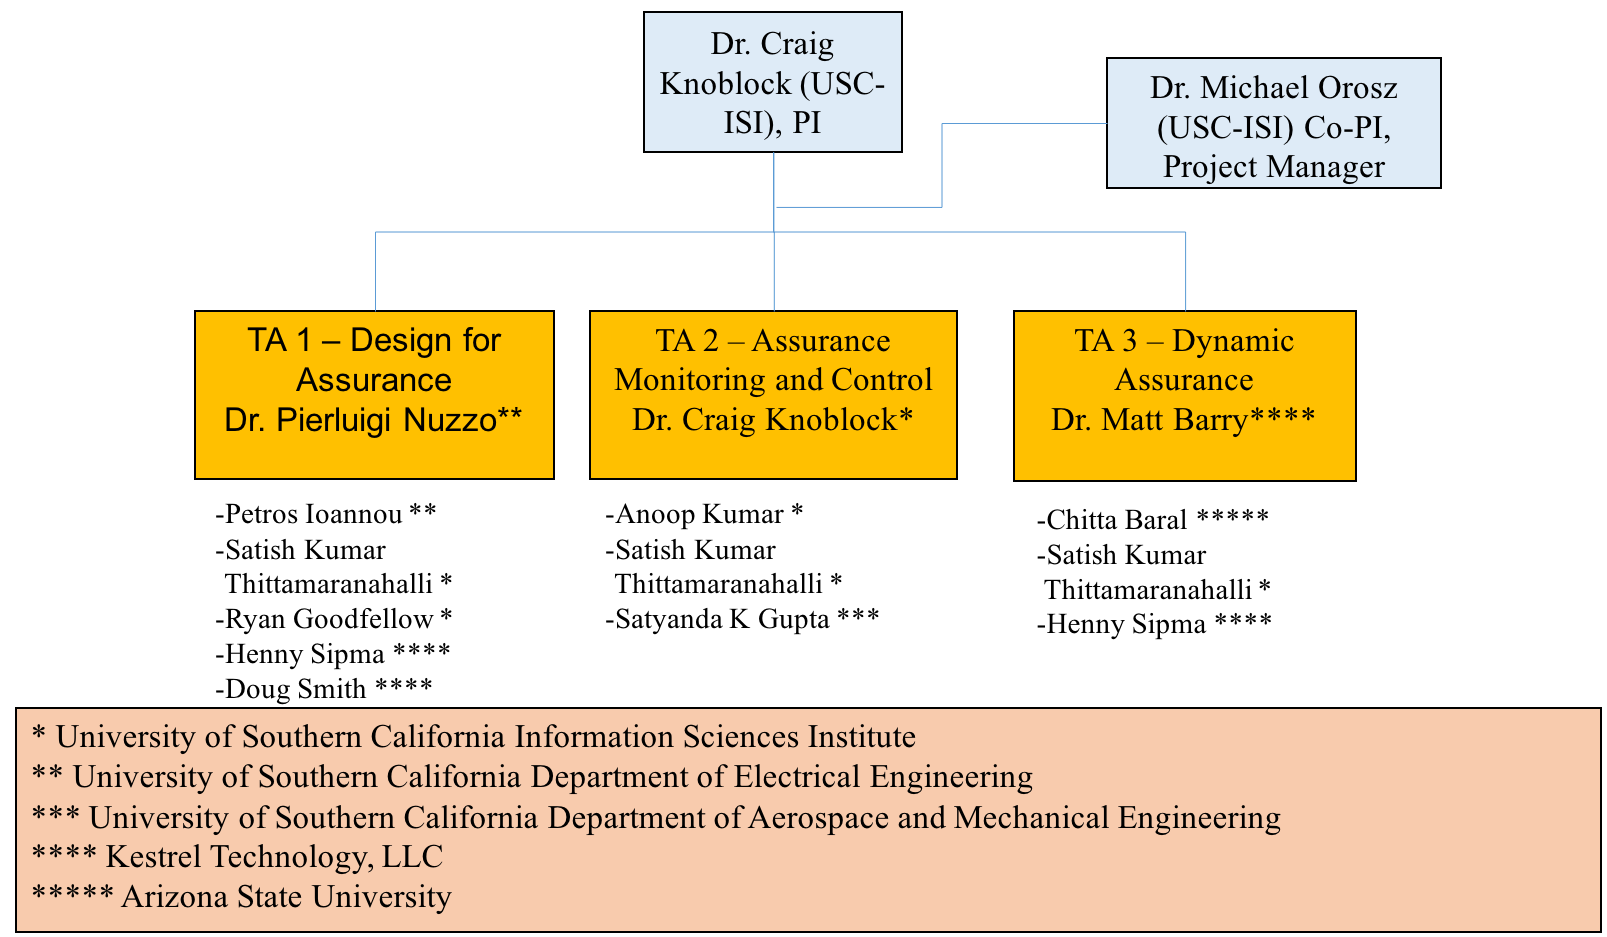
\includegraphics[width=6.0in]{./org-chart2.png}
\caption{\small Organization Chart}
\label{fig:org_chart}
\end{figure}

Coordination: To maximize collaboration and reduce risk to project failure from lack of communication and technical exchange, we plan to employ a wide variety of working styles and communication/coordination so that all can contribute.  At the core of our project will be regularly scheduled meetings bridging the diversely distributed team (Table~\ref{fig:Collaboration_Table}).  These meetings will address project status, identify challenges, implement risk mitigation strategies and participate in technology exchanges and system integration efforts (when appropriate)

\begin{table}[ht]
\caption{\small Project Meetings and Events}
  \centering
  {\footnotesize
\begin{tabular}{|m{3.15in}|m{3in}|} 
\hline
\textbf{Meeting} & \textbf{Frequency} 
\\\hline
Conference calls among investigators (discuss project status, address concerns and project risks) & Weekly
\\
\hline
Technical exchange and coordination meetings using Bluejeans or another videoconference technology & At least twice a month and more frequently as needed
  \\ 
\hline
Face-to-Face meetings (prior to P/I and demonstration meetings) & Every 3 to 6 months and more frequently (especially at the beginning of the project) as needed
 \\\cline{1-2}

\hline
\end{tabular}
}
\label{fig:Collaboration_Table}
\end{table}

\begin{table}[tbhp]
\caption{\small Key Project Team Member Responsibilities}
  \centering
  {\footnotesize
\begin{tabular}{| m{.75in} | m{3.9in}| m{1.5in}|} 
\hline
\textbf{Key Member} & \textbf{Responsibilities} & \textbf{Tasks} 
\\\hline
Dr.\ Craig Knoblock  & Principal Investigator responsible for project, leads TA 2 – Assurance Monitoring and Control.  Will lead the overall project and lead the TA2 team.  Served as the PI on many DARPA projects and has sucessfully led many large teams.    Effort on project:  25\% &
1.1.6, 1.2.2 1.2.3, 1.2.4, 1.3.4, 1.4.1, 
2.1.6, 2.2.2 2.2.3, 2.2.4, 2.3.4, 2.4.1, 
3.1.6, 3.2.2, 3.2.3, 3.2.4, 3.3.4, 3.4.1
\\
\hline
Dr.\ Michael Orosz & Co-Principal Investigator responsible managing the day-to-day operations of the project, assist technical teams as needed, coordinate with TA4 teams.    Has led many large complex multi-disciplined/multi-organizational projects in academic and industry environments.  Effort on project: 50\%
& 1.1.6, 2.1.6, 3.1.6, 1.4.1, 2.4.1, 3.4.1
  \\ 
\hline
Dr.\ Pierluigi Nuzzo 
& 
Co-Principal Investigator.  Leads the TA 1 - Design for Assurance team and conducts research on the formal methods for the design of the TA1 system.  Research experience on methodologies and tools for the design of cyber-physical systems; contracts, interfaces, and compositional methods for embedded system design; the application of automated formal methods and optimization theory to problems in embedded and cyber-physical systems.  Effort on project: 2 months/year (16.6\%)
& 
1.1.1, 2.1.1, 3.1.1 \\
\hline
Dr.\ Matthew Barry
& 
Key personnel.  Leads the TA 3 – Dynamic Assurance.   He will conduct the research on the dynamic assurance case language editors and parsers, the run-time system, and system integrations. Effort on project:  66\%
& 
1.3.2, 2.3.2, 3.3.2\\
\hline
Dr.\ Chitta Baral
& 
Key personnel responsible for learning assurance rules, supporting assurance rules with uncertainty and improving solver speed.  Expertise on ASP solvers, which will be used to reason about the assurance cases. Effort on project: 20\%
& 
1.3.1, 2.3.1, 3.3.1 \\
\hline
Dr.\ Doug Smith 
& 
Key personnel will support formal methods aspects of TA1, and lead the effort on abstract refinement. Expertise in field of automated correct-by-construction program generation.    Effort on project: 40\%
& 
1.1.5, 2.1.5, 3.1.5 \\
\hline
Dr.\ Henny Sipma
& 
Key personnel who will support the program verification tasks under TA1.  Will lead the effort on program verification.   Effort on project:  45\%
& 
1.1.5, 2.1.5, 3.1.5, 1.3.2, 2.3.2, 3.3.2 \\
\hline
Dr.\ Petros Ioannou
& 
Key personnel responsible providing and extending the assurance test bed, which will be available at the start of the project for autonomous vehicles.   Effort on project: 1 month/year (8.3\%)
& 
1.1.2, 2.1.2 (optional), 3.1.2 (optional)
\\
\hline
Dr.\ Satyandra Kumar Gupta
& 
Key Personnel providing autonomous command and control expertise to the TA-2 team.   Will lead the research on safety aware learning on TA2.   Past research on physics-aware decision making to facilitate automation.  Effort on project: 1 month/year (8.3\%)
& 
1.2.1, 2.2.1, 3.2.1 \\
\hline
Dr.\ Anoop Kumar 
& 
Key personnel providing support to the TA 2 project team.  Will lead the research on monitoring \& control and detecting distribution shifts.  Effort on project: 50\%
& 
1.2.1, 1.2.2, 1.2.3, 1.2.4, 2.2.1, 2.2.2, 2.2.3, 2.2.4, 3.2.1, 3.2.2, 3.2.3, 3.2.4\\
\hline
Dr.\ Satish Thittamaranahalli
& 
Key personnel developing scalable algorithms for TA1, TA2, and TA3 project teams.  Has extensive experience on scalable algorithm design, machine learning, and constraint reasoning.  Effort on project: 50\%
& 
1.2.1, 1.2.2, 1.2.3, 1.2.4, 2.2.1, 2.2.2, 2.2.3, 2.2.4, 3.2.1, 3.2.2, 3.2.3, 3.2.4, 1.1.4, 2.1.4, 3.1.4 \\
\hline
Dr.\ Ryan Goodfellow
& 
Key personnel providing support to the TA-1 project. Will lead the research on simulation-based testing.  Has extensive experience on simulation-based testing.  Effort on project:  30\%
& 
1.1.3, 2.1.3, 3.1.3 \\

\cline{1-2}

\hline
\end{tabular}
}
\label{fig:Table_Mgmt}
\end{table}



\newpage
\section{Personnel, Qualifications and Commitment}

{\bf Dr.\ Craig Knoblock}, the PI on this effort, is a Research Professor of both Computer Science and Spatial Sciences at the University of Southern California (USC) and Director of the Intelligent Systems Division at the USC Information Sciences Institute.   He received his Ph.D. from Carnegie Mellon University in computer science. 
%His research focuses on techniques for describing, acquiring, and exploiting the semantics of data.  
In previous projects he has worked on developing  scalable approaches to execution monitoring, accurate detection of sensor failures, and   automatic modeling and reconstruction of sensors.  He has published more than 300 journal articles, book chapters, and conference papers on these topics.  Dr. Knoblock is a Fellow of the Association for the Advancement of Artificial Intelligence (AAAI), a Distinguished Scientist of the Association of Computing Machinery (ACM), a Senior Member of IEEE, past President and Trustee of the International Joint Conference on Artificial Intelligence.
%and winner of the 2014 Robert S. Engelmore Award.  

{\bf Dr.\ Michael Orosz}, a Co-PI on this effort, is a Research Associate Professor of Civil and Environmental Engineering at the University of Southern California (USC) and Research Director of the Decision Systems Group at the USC Information Sciences Institute.  Dr. Orosz has over 30 years’ experience in commercial and government software development, basic and applied research, project management, academic research and has developed and deployed several commercially successful products.  His research interests are in machine learning and decision analytics as applied to intelligence analysis and autonomous command and control such as smart building controls.    Dr. Orosz has extensive experience in managing large complex multi-disciplined/multi-teamed research projects. %funded by DARPA, DHS, DoD, DoE, Industry, NASA, NRO, NSA and ONR.   
He received his Ph.D. in computer science from the University of California, Los Angeles.

{\bf Dr.\ Pierluigi Nuzzo}, a Co-PI on this project, is an Assistant Professor in the Department of Electrical Engineering at the University of Southern California. He received the Ph.D. in Electrical Engineering and Computer Sciences from the University of California at Berkeley. 
%in 2015, and the Laurea degree (MS) in electrical engineering (summa cum laude) from the University of Pisa, Italy, and the Sant'Anna School of Advanced Studies, Pisa, Italy.
%
%He has four years of research experience in analog and mixed signal circuit design as a researcher at IMEC, Leuven, Belgium, and over 10 years experience in design methodologies and tools for mixed-signal integrated circuits and cyber-physical systems, as a researcher at the University of Pisa, IMEC, UC Berkeley, and USC. 
His research interests
include: methodologies and tools for cyber-physical system and mixed-signal
system design; contracts, interfaces and compositional methods for embedded
system design; the application of formal methods and optimization theory to problems in embedded and cyber-physical systems and electronic design automation. 
%
Prof. Nuzzo received %First Place in the operational category and Best Overall
%Submission in the 2006 DAC/ISSCC Design Competition, 
a Marie Curie Fellowship
from the European Union in 2006, 
the University of California at Berkeley EECS
departmental fellowship in 2008, 
%the University of California at Berkeley Outstanding Graduate Student Instructor Award in 2013, 
the IBM Ph.D.
Fellowship in 2012 and 2014, 
%the Best Paper Award from the International Conference on Cyber-Physical Systems (ICCPS) in 2016, 
and the David J.~Sakrison Memorial Prize in 2016 for his doctoral research. 
%He is an author of 1 patent and over 60 publications.

{\bf Dr.\ Satyandra K. Gupta} is Smith International Professor in the Department of Aerospace and Mechanical Engineering at the University of Southern California. %Prior to joining the University of Southern California, he was a Professor in the Department of Mechanical Engineering and the Institute for Systems Research at the University of Maryland. He was the founding director of the Maryland Robotics Center and the Advanced Manufacturing Laboratory at the University of Maryland. 
He served as a program director for the National Robotics Initiative at the National Science Foundation from September 2012 to September 2014.  Dr. Gupta's interest is in the area of physics-aware decision making to facilitate automation. He has published more than 300 technical articles. He is a fellow of the American Society of Mechanical Engineers (ASME) and editor of ASME Journal of Computing and Information Science in Engineering. Dr. Gupta has received the Young Investigator Award from the Office of Naval Research in 2000, CAREER Award from the National Science Foundation in 2001, Presidential Early Career Award for Scientists and Engineers (PECASE) in 2001, Invention of the Year Award at the University of Maryland in 2007, Kos Ishii-Toshiba Award from ASME in 2011, and Excellence in Research Award from ASME in 2013.%, and Distinguished Alumnus Award from Indian Institute of Technology, Roorkee in 2014. %He has also received seven best paper awards at conferences.

{\bf Ryan Goodfellow} is a computer scientist at ISI working in combined cyber physical simulation and emulation platform development. His formal background is in simulation algorithms and modeling techniques using differential-algebraic equations (DAE). He has applied this knowledge in the CPS space by integrating DAE modeling languages and simulation engines with network testbeds to create comprehensive scientific experimentation platforms for cyber-physical systems. These experimentation platforms have been used in the power grid research space. %Ryan is a lead developer on the Deter network testbed, with a strong background in networked and distributed systems engineering. %He is also a combat veteran, serving as a non-commissioned officer and SIGINT team lead for a multi-functional intelligence team in Afghanistan.

{\bf Dr.\ Petros Ioannou} is a Professor in the Department of Electrical Engineering, Director of the Center for Advanced Transportation Technologies and Associate Director for Research for the DOT supported University Transportation Center at USC. He received his MS and PhD from the University of Illinois at Urbana Champaign in Mechanical and Electrical Engineering, respectively. His research interests are in robust adaptive control, vehicle dynamics and control, human factors and safety, automated vehicles, nonlinear systems and Intelligent transportation Systems.  He received the 2016 IEEE Transportation Technologies field award and the 2016 IEEE Control system society Transition to Practice Award. He is a Fellow of IEEE, IFAC and IET and author/coauthor of 8 books and over 400 papers.

{\bf Dr.\ Matthew Barry} will serve as lead for the TA3 tasks. %He will implement the dynamic assurance case language editors and parsers, the run-time system, and system integrations.  He will implement the assurance case arguments and the API for updating argument structure and content.  
Dr. Barry currently is CEO at Kestrel Technology LLC, and previously spent 20 years in NASA space mission operations at the Jet Propulsion Lab and Johnson Space Center.  At NASA Headquarters he led the introduction of dependability case requirements and plans for flight computing systems in upcoming manned space exploration missions, as well as the development of Agency-level software-related safety-critical control system requirements.  He recently served as a Principal Investigator on DHS/Cyber S\&T STAMP (Static Tool Analysis Modernization Program), DARPA CSFV (Crowd Sourced Formal Verification), three NASA Aeronautics R\&D projects, and the AFRL-sponsored Static Analysis of Numerical Algorithms project.  Dr. Barry earned BSME, MS, and PhD degrees in mechanical engineering, and an MBA degree, from Rice University.  

{\bf Dr.\ Henny Sipma} will support the program verification tasks under TA1.  %She is the key person behind the company's {\em KT Advance\/} and {\em KT Transferal\/} static analysis products, and the designer and programmer of the company's core {\em CodeHawk\/} abstract interpretation engine. 
Dr. Sipma currently is the CTO at Kestrel Technology LLC.  She has spent the past 10 years with Kestrel Technology as a static analysis expert; previously developed and taught static analysis techniques as senior research associate at Stanford University for eight years; and developed industrial process controls as an senior systems analyst at Shell.  She has been Principal Investigator or company lead on several recent R\&D projects for Federal agencies, including two projects under the IARPA STONESOUP (Securely Taking On New Executable Software of Uncertain Provenance) program; the DHS Cyber S\&T Gold Standard project; and the DARPA-sponsored STAC (Space-Time Analysis for Cybersecurity) and MUSE (Mining and Understanding Software Enclaves) programs.  Dr. Sipma earned 
%a BS degree in chemistry and an MS degree in chemical engineering at the University of Groningen in The Netherlands, and 
MS and PhD degrees in computer science from Stanford University.  

{\bf Dr.\ Douglas R.\ Smith} will support formal methods aspects of TA1, including the enforcement of safety properties and the generation of monitors.  He is President of Kestrel Technology LLC and Principal Scientist at Kestrel Institute.  He is a Fellow of the American Association of Artificial Intelligence (AAAI) and an ASE Fellow (Automated Software Engineering).  From 1986 to 2000, he taught an advanced graduate course on correct-by-construction software development at Stanford.  
%Dr. Smith has led the development of a series of software synthesis systems, including KIDS (Kestrel Interactive Development System), Specware, Designware, and Planware. 
%Applications domains have included a variety of complex high-performance planners and schedulers for the US Air Force.  He leads current projects on the generation of air mission plans and cyberoperations.  
Other recent projects focused on automated policy enforcement \cite{SmithD0703,SmithD08}, synthesis of secure network protocol codes, and the synthesis of high-performance constraint-solvers\cite{SmithD08c,SmithD13}.  Dr. Smith has over 30 years experience in the field of automated correct-by-construction program generation and has published over 100 papers. He has one patent.  He received the Ph.D. in Computer Science from Duke University% in 1979.  

{\bf Dr. Chitta Baral} is a Professor in the Department of Computer Science and Engineering at Arizona State University. He will support the TA3 efforts on Learning assurance rules, supporting assurance rules with uncertainty and improving solver speed. Dr. Baral has expertise in various aspects of autonomy and Artificial Intelligence. 
He wrote the first book on answer set programming (published by Cambridge University Press) the formal language behind our assurance rules. Some of his other works relevant to this proposal are: goal specification for autonomous systems, automatic construction of control rules for autonomous systems that satisfy given goals, combining machine learning with reasoning in various contexts, including image understanding. %He is the President of KR Inc. He is an associate editor of AIJ and has been an associate editor of JAIR.

{\bf Dr.\ Satish Kumar Thittamaranahalli (T. K. Satish Kumar)} leads the Collaboratory for Algorithmic Techniques and Artificial Intelligence (CATAI) at USC's Information Sciences Institute. He has published over 60 papers on numerous topics in Artificial Intelligence spanning such diverse areas as Constraint Reasoning, Planning and Scheduling, Probabilistic Reasoning, Robotics, Combinatorial Optimization, Approximation and Randomization, Heuristic Search, Model-Based Reasoning, Knowledge Representation and Spatio-Temporal Reasoning. %He %has served on the Program Committees of many international conferences in Artificial Intelligence
He and is a winner of the 2016 Best Robotics Paper Award and the 2005 Best Student Paper Award from the International Conference on Automated Planning and Scheduling. 
Dr. Kumar received his PhD in Computer Science from Stanford University. %In the past, he has also been a Visiting Student at the NASA Ames Research Center, a Postdoctoral Research Scholar at the University of California, Berkeley, a Research Scientist at the Institute for Human and Machine Cognition, a Visiting Assistant Professor at the University of West Florida, and a Senior Research and Development Scientist at Mission Critical Technologies.

\textbf{Dr.\ Anoop Kumar} is a senior computer scientist at USC ISI and has broad expertise in machine learning, statistical modeling, and software engineering.  Dr.\ Kumar is the technical lead on the DARPA RSPACE program and has played a vital role in developing a system that fuses air operations data from multiple sources, maintains world state, and issues warnings. Previously, he led the research and development of the BBN’s election forecasting system for the IARPA OSI program. %Dr.\ Kumar played a significant role in the DARPA DEFT program by developing a model to support integration of output from multiple NLP algorithms. He has contributed at the development to management levels on government research contracts and commercial projects. 
Dr.\ Kumar helped design and develop BBN's commercially available, hosted speech and medical transcription services offering. 

\begin{table}[!tbh]
\begin{footnotesize}
\vspace{-0.1in}

\begin{tabular}{lll}
\begin{tabular}[t]{|l|@{}c@{}|@{}c@{}|@{}c@{}|@{}c@{}|} \hline
Project & Status & \multicolumn{3}{ c| }{Hours} \\ \cline{3-5}
& & P1 & P2 & P3 \\ \hline



\multicolumn{5}{ |c| }{ \textbf{Craig Knoblock} } \\ \cline{1-5}
Safeguard & Pro & 770 & 641 & 641 \\ \cline{1-5}
ELICIT & Cur & 308 & 256 & 120 \\ \cline{1-5}
WTNIC & Cur & 11 & 0 & 0 \\ \cline{1-5}
EFFECT & Cur & 641 & 107 & 0 \\ \cline{1-5}
LinkedMaps & Cur & 203 & 25 & 0 \\ \cline{1-5}
PRINCESS & Cur & 608 & 96 & 0 \\ \cline{1-5}
SCHARP & Cur & 481 & 54 & 0 \\ \cline{1-5}
MINT & Pen & 650 & 534 & 285 \\ \cline{1-5}

\multicolumn{5}{ |c| }{ \textbf{Michael Orosz} } \\ \cline{1-5}
Safeguard & Pro & 1560 & 1300 & 1300  \\ \cline{1-5}
SMC/SY & Cur & 1803 & 0 & 0  \\ \cline{1-5}

\multicolumn{5}{ |c| }{ \textbf{Matthew Barry} } \\ \cline{1-5}
Safeguard & Pro & 2078 & 1690 & 1554 \\ \cline{1-5}
Starlite & Cur & 1840 & 1692 & 0 \\ \cline{1-5}



\multicolumn{5}{ |c| }{ \textbf{Anoop Kumar} } \\ \cline{1-5}
Safeguard & Pro & 1560 & 1300 & 1300 \\ \cline{1-5}

\end{tabular}
&
\begin{tabular}[t]{|l|@{}c@{}|@{}c@{}|@{}c@{}|@{}c@{}|} \hline
Project & Status & \multicolumn{3}{ c| }{Hours} \\ \cline{3-5}
& & P1 & P2 & P3 \\ \hline

\multicolumn{5}{ |c| }{ \textbf{Pierluigi Nuzzo} } \\ \cline{1-5}
Safeguard & Pro & 520 & 433 & 433  \\ \cline{1-5}
Mirage & Cur & 433 & 0 & 0  \\ \cline{1-5}

\multicolumn{5}{ |c| }{ \textbf{Satyandra Gupta} } \\ \cline{1-5}
Safeguard & Pro & 260 & 217 & 217 \\ \cline{1-5}
Human   & Cur & 22 & 0 & 0 \\ \cline{1-5}
Vehicles & Cur & 36 & 0 & 0 \\ \cline{1-5}
Robot & Cur & 116 & 0 & 0 \\ \cline{1-5}
Assembly & Cur & 33 & 0 & 0 \\ \cline{1-5}
Solar & Cur & 4 & 0 & 0 \\ \cline{1-5}

\multicolumn{5}{ |c| }{ \textbf{Petros Ioannou} } \\ \cline{1-5}
Safeguard & Pro & 260 & 217 & 217 \\ \cline{1-5}
CPS & Cur & 130 & 0 & 0 \\ \cline{1-5}

\multicolumn{5}{ |c| }{ \textbf{Ryan Goodfellow} } \\ \cline{1-5}
Safeguard & Pro & 936 & 780 & 780 \\ \cline{1-5}
STEAM & Cur & 416 & 0 & 0 \\ \cline{1-5}


\end{tabular}
&
\begin{tabular}[t]{|l|@{}c@{}|@{}c@{}|@{}c@{}|@{}c@{}|} \hline
Project & Status & \multicolumn{3}{ c| }{Hours} \\ \cline{3-5}
& & P1 & P2 & P3 \\ \hline

\multicolumn{5}{ |c| }{ \textbf{Chitta Baral} } \\ \cline{1-5}
Safeguard & Pro & 659 & 485 & 485 \\ \cline{1-5}
PostdocBP & Cur & 176 & 0 & 0 \\ \cline{1-5}
Languages & Pen & 528 & 264 & 264 \\ \cline{1-5}
CAREER & Pen & 88 & 44 & 44 \\ \cline{1-5}
CHS & Pen & 510 & 255 & 0 \\ \cline{1-5}

\multicolumn{5}{ |c| }{ \textbf{Doug Smith} } \\ \cline{1-5}
Safeguard & Pro & 1222 & 984 & 840 \\ \cline{1-5}
RSPACE & Cur & 342 & 0 & 0 \\ 
\cline{1-5}
PLANX & Cur & 154 & 0 & 0 \\ 
\cline{1-5}
HACCS & Pen & 923 & 769 & 769 \\ 
\cline{1-5}

\multicolumn{5}{ |c| }{ \textbf{Henny Sipma} } \\ \cline{1-5}
Safeguard & Pro & 1372 & 962 & 840 \\ \cline{1-5}
STAC & Cur & 797 & 0 & 0 \\ \cline{1-5}

\multicolumn{5}{ |c| }{ \textbf{Satish Thittamaranahalli} } \\ \cline{1-5}
Safeguard & Pro & 1560 & 1300 & 1300 \\ \cline{1-5}
MapF & Cur & 103 & 103 & 0 \\ \cline{1-5}

\end{tabular}
\end{tabular}

\end{footnotesize}
\caption{Individual commitments of key personnel}
\label{tab:Commitments}
\vspace{-0.2in}
\end{table}

\clearpage
\newpage
\section{Capabilities}


%\subsection{University of Southern California}
USC has strengths in number of areas that are closely related to the proposed work:
\begin{itemize}[itemsep=0pt,leftmargin=*]
\item Dr.\ Nuzzo 
%has over 10-year research experience in embedded system design, from mixed-signal chip design (analog-to-digital converters, frequency synthesizers, software-defined radio), to methodologies and tools for mixed-signal integrated circuits and Cyber-Physical Systems (CPSs), and the application of formal methods and optimization theory to problems in embedded and cyber-physical systems and electronic design automation.  
%His doctoral work 
has done extensive research on contracts and compositional methods for heterogeneous system design and design space exploration, with application to aircraft electric power systems and environmental control systems. His work has helped transition rigorous system design foundations, innovative design methodologies, and new systems engineering paradigms to industry (IBM, United Technologies). 
\item Dr.\ Satyandra K. Gupta has worked on autonomous surface vehicles, autonomous ground vehicles for operation on rugged terrains, and autonomous flapping wing aerial vehicles.   His group has developed a hierarchal decision making approach for realizing autonomous systems. 
%This approach combines task planning and assignment, deliberative trajectory planning, reactive collision avoidance behaviors, and trajectory tracking control layers. 
His group has also developed new methods for learning reactive behaviors in adversarial environments and COLREGS compliant trajectory planning. \item Dr.\ Knoblock has developed methods that learn the relationships between sensors to both identify failures and changes in sensor and reconstruct those sensors, providing estimates of the accuracy of the reconstructed sensors.  
\item Ryan Goodfellow has extensive experience in simulation based testing through high-fidelity CPS testbed environment development and operation, using the Deter network testbed as the core which has supported several large scale government projects from a variety of agencies and thousands of users. %we have developed sophisticated CPS experiments under programs such as NFS RIPS, NIST SmartCities and the DHS Cybersecurity showcase.
\item Dr.\ Ioannou %helped  design and implement adaptive cruise control systems in collaboration with Ford Motor Company, which was commercialized four years before any other company. He 
worked on several DOT funded projects on automated vehicles and intelligent highway systems where he demonstrated his vehicle control designs for safety and performance on actual automated vehicles in test trucks and I-15 highway.
\item Drs.\ Knoblock, Kumar, and Thittamaranahalli have developed highly scalable approaches for monitoring message traffic to identify potential problems and issue warnings and alerts. 
\item Dr. Thittamaranahalli has developed state-of-the-art methods for efficiently solving large-scale search and optimization problems. %These techniques will be applicable in TA2 for safety-aware learning and planning, in TA2 for assurance monitoring and control, and in TA3 for dynamic assessment of assurance cases.

\end{itemize}
%\subsection{Kestrel Technology LLC}

Kestrel Technology's strength is in program analysis, specifically static analysis of both source and binary targets.  The company performs applied R\&D and product development for a variety of static analysis applications  pivoting primarily on the abstract interpretation technique.  The company recently initiated development of program analysis applications using logical equivalence techniques. As a provider of verification evidence in the form of mathematical proofs, the company also has expertise in the design and development of assurance case arguments for high-integrity systems using such evidence. %The company is engaged in a partnership with Wind River Systems to develop program analysis tools for its embedded system developers.  Many of Wind River's customers must develop their products under safety and certification standards, including those using safety cases.  

   

%\subsection{Arizona State University}
Chitta Baral at Arizona State University has developed various software to learn assurance rules and various ASP solvers, which he has made available as open-source.

Most of the software carried forward for implementation or derivation is open source.  The single exception is Kestrel Technology's {\it KT Advance\/} static analysis tool (TA1), in particular the abstract interpretation engine therein, which is company proprietary and is US EAR export-controlled.   
%Owing to mixed funding for the development of that technology 
We will continue to provide the Federal government a restricted use license for that particular item.

There are no specialized facilities, data, or GFE required for this effort. 

\include{sow}
\include{milestones}

% \section{Level of Effort by Task \textcolor{red}{[Mike/Lisa - 1 pages]}}

% \textcolor{blue}{
% \begin{itemize}
% \item Will be a separate spreadsheet
% \item
% \end{itemize}
% }

\include{appendix_a}

%\section{Appendix B \textcolor{red}{[No Page Count]}}

\section{References}
\bibliographystyle{acm} 
\bibliography{TA3/ta3,TA2/ta2,TA1/ta1}
\end{document}
\clearpage
\newpage


\section{Management Plan}


The Principal Investigator for this effort is Dr. Craig Knoblock who is responsible for all aspects of the effort, will coordinate the parallel team efforts, and will ensure high levels of performance from individual team members.  The Co-P/I, Dr. Michael Orosz, will provide project management and will assist all performers in the execution of the project.    The project team is divided into three working groups (Figure~\ref{fig:org_chart}) corresponding to Technical Areas 1-3, however, members of each team contribute across all project activities.   Table~\ref{fig:Table_Mgmt} defines the major contributions of each project team member to the project tasks.

\begin{figure}[tbhp]
%\vspace{-25pt}
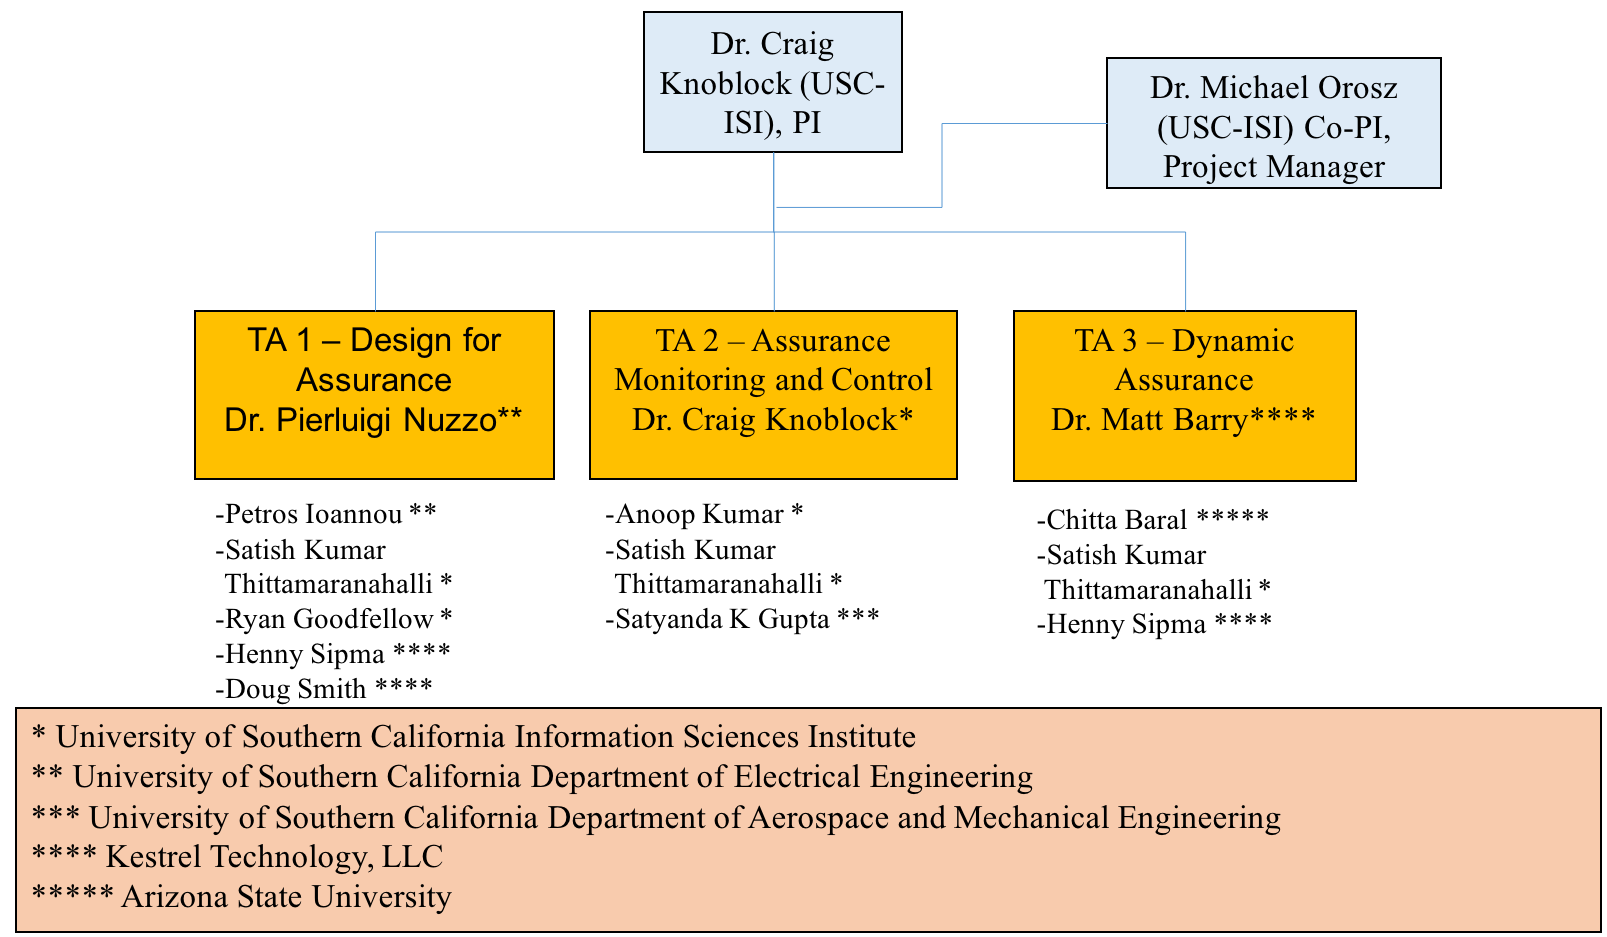
\includegraphics[width=6.0in]{./org-chart2.png}
\caption{\small Organization Chart}
\label{fig:org_chart}
\end{figure}

Coordination: To maximize collaboration and reduce risk to project failure from lack of communication and technical exchange, we plan to employ a wide variety of working styles and communication/coordination so that all can contribute.  At the core of our project will be regularly scheduled meetings bridging the diversely distributed team (Table~\ref{fig:Collaboration_Table}).  These meetings will address project status, identify challenges, implement risk mitigation strategies and participate in technology exchanges and system integration efforts (when appropriate)

\begin{table}[ht]
\caption{\small Project Meetings and Events}
  \centering
  {\footnotesize
\begin{tabular}{|m{3.15in}|m{3in}|} 
\hline
\textbf{Meeting} & \textbf{Frequency} 
\\\hline
Conference calls among investigators (discuss project status, address concerns and project risks) & Weekly
\\
\hline
Technical exchange and coordination meetings using Bluejeans or another videoconference technology & At least twice a month and more frequently as needed
  \\ 
\hline
Face-to-Face meetings (prior to P/I and demonstration meetings) & Every 3 to 6 months and more frequently (especially at the beginning of the project) as needed
 \\\cline{1-2}

\hline
\end{tabular}
}
\label{fig:Collaboration_Table}
\end{table}

\begin{table}[tbhp]
\caption{\small Key Project Team Member Responsibilities}
  \centering
  {\footnotesize
\begin{tabular}{| m{.75in} | m{3.9in}| m{1.5in}|} 
\hline
\textbf{Key Member} & \textbf{Responsibilities} & \textbf{Tasks} 
\\\hline
Dr.\ Craig Knoblock  & Principal Investigator responsible for project, leads TA 2 – Assurance Monitoring and Control.  Will lead the overall project and lead the TA2 team.  Served as the PI on many DARPA projects and has sucessfully led many large teams.    Effort on project:  25\% &
1.1.6, 1.2.2 1.2.3, 1.2.4, 1.3.4, 1.4.1, 
2.1.6, 2.2.2 2.2.3, 2.2.4, 2.3.4, 2.4.1, 
3.1.6, 3.2.2, 3.2.3, 3.2.4, 3.3.4, 3.4.1
\\
\hline
Dr.\ Michael Orosz & Co-Principal Investigator responsible managing the day-to-day operations of the project, assist technical teams as needed, coordinate with TA4 teams.    Has led many large complex multi-disciplined/multi-organizational projects in academic and industry environments.  Effort on project: 50\%
& 1.1.6, 2.1.6, 3.1.6, 1.4.1, 2.4.1, 3.4.1
  \\ 
\hline
Dr.\ Pierluigi Nuzzo 
& 
Co-Principal Investigator.  Leads the TA 1 - Design for Assurance team and conducts research on the formal methods for the design of the TA1 system.  Research experience on methodologies and tools for the design of cyber-physical systems; contracts, interfaces, and compositional methods for embedded system design; the application of automated formal methods and optimization theory to problems in embedded and cyber-physical systems.  Effort on project: 2 months/year (16.6\%)
& 
1.1.1, 2.1.1, 3.1.1 \\
\hline
Dr.\ Matthew Barry
& 
Key personnel.  Leads the TA 3 – Dynamic Assurance.   He will conduct the research on the dynamic assurance case language editors and parsers, the run-time system, and system integrations. Effort on project:  66\%
& 
1.3.2, 2.3.2, 3.3.2\\
\hline
Dr.\ Chitta Baral
& 
Key personnel responsible for learning assurance rules, supporting assurance rules with uncertainty and improving solver speed.  Expertise on ASP solvers, which will be used to reason about the assurance cases. Effort on project: 20\%
& 
1.3.1, 2.3.1, 3.3.1 \\
\hline
Dr.\ Doug Smith 
& 
Key personnel will support formal methods aspects of TA1, and lead the effort on abstract refinement. Expertise in field of automated correct-by-construction program generation.    Effort on project: 40\%
& 
1.1.5, 2.1.5, 3.1.5 \\
\hline
Dr.\ Henny Sipma
& 
Key personnel who will support the program verification tasks under TA1.  Will lead the effort on program verification.   Effort on project:  45\%
& 
1.1.5, 2.1.5, 3.1.5, 1.3.2, 2.3.2, 3.3.2 \\
\hline
Dr.\ Petros Ioannou
& 
Key personnel responsible providing and extending the assurance test bed, which will be available at the start of the project for autonomous vehicles.   Effort on project: 1 month/year (8.3\%)
& 
1.1.2, 2.1.2 (optional), 3.1.2 (optional)
\\
\hline
Dr.\ Satyandra Kumar Gupta
& 
Key Personnel providing autonomous command and control expertise to the TA-2 team.   Will lead the research on safety aware learning on TA2.   Past research on physics-aware decision making to facilitate automation.  Effort on project: 1 month/year (8.3\%)
& 
1.2.1, 2.2.1, 3.2.1 \\
\hline
Dr.\ Anoop Kumar 
& 
Key personnel providing support to the TA 2 project team.  Will lead the research on monitoring \& control and detecting distribution shifts.  Effort on project: 50\%
& 
1.2.1, 1.2.2, 1.2.3, 1.2.4, 2.2.1, 2.2.2, 2.2.3, 2.2.4, 3.2.1, 3.2.2, 3.2.3, 3.2.4\\
\hline
Dr.\ Satish Thittamaranahalli
& 
Key personnel developing scalable algorithms for TA1, TA2, and TA3 project teams.  Has extensive experience on scalable algorithm design, machine learning, and constraint reasoning.  Effort on project: 50\%
& 
1.2.1, 1.2.2, 1.2.3, 1.2.4, 2.2.1, 2.2.2, 2.2.3, 2.2.4, 3.2.1, 3.2.2, 3.2.3, 3.2.4, 1.1.4, 2.1.4, 3.1.4 \\
\hline
Dr.\ Ryan Goodfellow
& 
Key personnel providing support to the TA-1 project. Will lead the research on simulation-based testing.  Has extensive experience on simulation-based testing.  Effort on project:  30\%
& 
1.1.3, 2.1.3, 3.1.3 \\

\cline{1-2}

\hline
\end{tabular}
}
\label{fig:Table_Mgmt}
\end{table}



\newpage
\section{Personnel, Qualifications and Commitment}

{\bf Dr.\ Craig Knoblock}, the PI on this effort, is a Research Professor of both Computer Science and Spatial Sciences at the University of Southern California (USC) and Director of the Intelligent Systems Division at the USC Information Sciences Institute.   He received his Ph.D. from Carnegie Mellon University in computer science. 
%His research focuses on techniques for describing, acquiring, and exploiting the semantics of data.  
In previous projects he has worked on developing  scalable approaches to execution monitoring, accurate detection of sensor failures, and   automatic modeling and reconstruction of sensors.  He has published more than 300 journal articles, book chapters, and conference papers on these topics.  Dr. Knoblock is a Fellow of the Association for the Advancement of Artificial Intelligence (AAAI), a Distinguished Scientist of the Association of Computing Machinery (ACM), a Senior Member of IEEE, past President and Trustee of the International Joint Conference on Artificial Intelligence.
%and winner of the 2014 Robert S. Engelmore Award.  

{\bf Dr.\ Michael Orosz}, a Co-PI on this effort, is a Research Associate Professor of Civil and Environmental Engineering at the University of Southern California (USC) and Research Director of the Decision Systems Group at the USC Information Sciences Institute.  Dr. Orosz has over 30 years’ experience in commercial and government software development, basic and applied research, project management, academic research and has developed and deployed several commercially successful products.  His research interests are in machine learning and decision analytics as applied to intelligence analysis and autonomous command and control such as smart building controls.    Dr. Orosz has extensive experience in managing large complex multi-disciplined/multi-teamed research projects. %funded by DARPA, DHS, DoD, DoE, Industry, NASA, NRO, NSA and ONR.   
He received his Ph.D. in computer science from the University of California, Los Angeles.

{\bf Dr.\ Pierluigi Nuzzo}, a Co-PI on this project, is an Assistant Professor in the Department of Electrical Engineering at the University of Southern California. He received the Ph.D. in Electrical Engineering and Computer Sciences from the University of California at Berkeley. 
%in 2015, and the Laurea degree (MS) in electrical engineering (summa cum laude) from the University of Pisa, Italy, and the Sant'Anna School of Advanced Studies, Pisa, Italy.
%
%He has four years of research experience in analog and mixed signal circuit design as a researcher at IMEC, Leuven, Belgium, and over 10 years experience in design methodologies and tools for mixed-signal integrated circuits and cyber-physical systems, as a researcher at the University of Pisa, IMEC, UC Berkeley, and USC. 
His research interests
include: methodologies and tools for cyber-physical system and mixed-signal
system design; contracts, interfaces and compositional methods for embedded
system design; the application of formal methods and optimization theory to problems in embedded and cyber-physical systems and electronic design automation. 
%
Prof. Nuzzo received %First Place in the operational category and Best Overall
%Submission in the 2006 DAC/ISSCC Design Competition, 
a Marie Curie Fellowship
from the European Union in 2006, 
the University of California at Berkeley EECS
departmental fellowship in 2008, 
%the University of California at Berkeley Outstanding Graduate Student Instructor Award in 2013, 
the IBM Ph.D.
Fellowship in 2012 and 2014, 
%the Best Paper Award from the International Conference on Cyber-Physical Systems (ICCPS) in 2016, 
and the David J.~Sakrison Memorial Prize in 2016 for his doctoral research. 
%He is an author of 1 patent and over 60 publications.

{\bf Dr.\ Satyandra K. Gupta} is Smith International Professor in the Department of Aerospace and Mechanical Engineering at the University of Southern California. %Prior to joining the University of Southern California, he was a Professor in the Department of Mechanical Engineering and the Institute for Systems Research at the University of Maryland. He was the founding director of the Maryland Robotics Center and the Advanced Manufacturing Laboratory at the University of Maryland. 
He served as a program director for the National Robotics Initiative at the National Science Foundation from September 2012 to September 2014.  Dr. Gupta's interest is in the area of physics-aware decision making to facilitate automation. He has published more than 300 technical articles. He is a fellow of the American Society of Mechanical Engineers (ASME) and editor of ASME Journal of Computing and Information Science in Engineering. Dr. Gupta has received the Young Investigator Award from the Office of Naval Research in 2000, CAREER Award from the National Science Foundation in 2001, Presidential Early Career Award for Scientists and Engineers (PECASE) in 2001, Invention of the Year Award at the University of Maryland in 2007, Kos Ishii-Toshiba Award from ASME in 2011, and Excellence in Research Award from ASME in 2013.%, and Distinguished Alumnus Award from Indian Institute of Technology, Roorkee in 2014. %He has also received seven best paper awards at conferences.

{\bf Ryan Goodfellow} is a computer scientist at ISI working in combined cyber physical simulation and emulation platform development. His formal background is in simulation algorithms and modeling techniques using differential-algebraic equations (DAE). He has applied this knowledge in the CPS space by integrating DAE modeling languages and simulation engines with network testbeds to create comprehensive scientific experimentation platforms for cyber-physical systems. These experimentation platforms have been used in the power grid research space. %Ryan is a lead developer on the Deter network testbed, with a strong background in networked and distributed systems engineering. %He is also a combat veteran, serving as a non-commissioned officer and SIGINT team lead for a multi-functional intelligence team in Afghanistan.

{\bf Dr.\ Petros Ioannou} is a Professor in the Department of Electrical Engineering, Director of the Center for Advanced Transportation Technologies and Associate Director for Research for the DOT supported University Transportation Center at USC. He received his MS and PhD from the University of Illinois at Urbana Champaign in Mechanical and Electrical Engineering, respectively. His research interests are in robust adaptive control, vehicle dynamics and control, human factors and safety, automated vehicles, nonlinear systems and Intelligent transportation Systems.  He received the 2016 IEEE Transportation Technologies field award and the 2016 IEEE Control system society Transition to Practice Award. He is a Fellow of IEEE, IFAC and IET and author/coauthor of 8 books and over 400 papers.

{\bf Dr.\ Matthew Barry} will serve as lead for the TA3 tasks. %He will implement the dynamic assurance case language editors and parsers, the run-time system, and system integrations.  He will implement the assurance case arguments and the API for updating argument structure and content.  
Dr. Barry currently is CEO at Kestrel Technology LLC, and previously spent 20 years in NASA space mission operations at the Jet Propulsion Lab and Johnson Space Center.  At NASA Headquarters he led the introduction of dependability case requirements and plans for flight computing systems in upcoming manned space exploration missions, as well as the development of Agency-level software-related safety-critical control system requirements.  He recently served as a Principal Investigator on DHS/Cyber S\&T STAMP (Static Tool Analysis Modernization Program), DARPA CSFV (Crowd Sourced Formal Verification), three NASA Aeronautics R\&D projects, and the AFRL-sponsored Static Analysis of Numerical Algorithms project.  Dr. Barry earned BSME, MS, and PhD degrees in mechanical engineering, and an MBA degree, from Rice University.  

{\bf Dr.\ Henny Sipma} will support the program verification tasks under TA1.  %She is the key person behind the company's {\em KT Advance\/} and {\em KT Transferal\/} static analysis products, and the designer and programmer of the company's core {\em CodeHawk\/} abstract interpretation engine. 
Dr. Sipma currently is the CTO at Kestrel Technology LLC.  She has spent the past 10 years with Kestrel Technology as a static analysis expert; previously developed and taught static analysis techniques as senior research associate at Stanford University for eight years; and developed industrial process controls as an senior systems analyst at Shell.  She has been Principal Investigator or company lead on several recent R\&D projects for Federal agencies, including two projects under the IARPA STONESOUP (Securely Taking On New Executable Software of Uncertain Provenance) program; the DHS Cyber S\&T Gold Standard project; and the DARPA-sponsored STAC (Space-Time Analysis for Cybersecurity) and MUSE (Mining and Understanding Software Enclaves) programs.  Dr. Sipma earned 
%a BS degree in chemistry and an MS degree in chemical engineering at the University of Groningen in The Netherlands, and 
MS and PhD degrees in computer science from Stanford University.  

{\bf Dr.\ Douglas R.\ Smith} will support formal methods aspects of TA1, including the enforcement of safety properties and the generation of monitors.  He is President of Kestrel Technology LLC and Principal Scientist at Kestrel Institute.  He is a Fellow of the American Association of Artificial Intelligence (AAAI) and an ASE Fellow (Automated Software Engineering).  From 1986 to 2000, he taught an advanced graduate course on correct-by-construction software development at Stanford.  
%Dr. Smith has led the development of a series of software synthesis systems, including KIDS (Kestrel Interactive Development System), Specware, Designware, and Planware. 
%Applications domains have included a variety of complex high-performance planners and schedulers for the US Air Force.  He leads current projects on the generation of air mission plans and cyberoperations.  
Other recent projects focused on automated policy enforcement \cite{SmithD0703,SmithD08}, synthesis of secure network protocol codes, and the synthesis of high-performance constraint-solvers\cite{SmithD08c,SmithD13}.  Dr. Smith has over 30 years experience in the field of automated correct-by-construction program generation and has published over 100 papers. He has one patent.  He received the Ph.D. in Computer Science from Duke University% in 1979.  

{\bf Dr. Chitta Baral} is a Professor in the Department of Computer Science and Engineering at Arizona State University. He will support the TA3 efforts on Learning assurance rules, supporting assurance rules with uncertainty and improving solver speed. Dr. Baral has expertise in various aspects of autonomy and Artificial Intelligence. 
He wrote the first book on answer set programming (published by Cambridge University Press) the formal language behind our assurance rules. Some of his other works relevant to this proposal are: goal specification for autonomous systems, automatic construction of control rules for autonomous systems that satisfy given goals, combining machine learning with reasoning in various contexts, including image understanding. %He is the President of KR Inc. He is an associate editor of AIJ and has been an associate editor of JAIR.

{\bf Dr.\ Satish Kumar Thittamaranahalli (T. K. Satish Kumar)} leads the Collaboratory for Algorithmic Techniques and Artificial Intelligence (CATAI) at USC's Information Sciences Institute. He has published over 60 papers on numerous topics in Artificial Intelligence spanning such diverse areas as Constraint Reasoning, Planning and Scheduling, Probabilistic Reasoning, Robotics, Combinatorial Optimization, Approximation and Randomization, Heuristic Search, Model-Based Reasoning, Knowledge Representation and Spatio-Temporal Reasoning. %He %has served on the Program Committees of many international conferences in Artificial Intelligence
He and is a winner of the 2016 Best Robotics Paper Award and the 2005 Best Student Paper Award from the International Conference on Automated Planning and Scheduling. 
Dr. Kumar received his PhD in Computer Science from Stanford University. %In the past, he has also been a Visiting Student at the NASA Ames Research Center, a Postdoctoral Research Scholar at the University of California, Berkeley, a Research Scientist at the Institute for Human and Machine Cognition, a Visiting Assistant Professor at the University of West Florida, and a Senior Research and Development Scientist at Mission Critical Technologies.

\textbf{Dr.\ Anoop Kumar} is a senior computer scientist at USC ISI and has broad expertise in machine learning, statistical modeling, and software engineering.  Dr.\ Kumar is the technical lead on the DARPA RSPACE program and has played a vital role in developing a system that fuses air operations data from multiple sources, maintains world state, and issues warnings. Previously, he led the research and development of the BBN’s election forecasting system for the IARPA OSI program. %Dr.\ Kumar played a significant role in the DARPA DEFT program by developing a model to support integration of output from multiple NLP algorithms. He has contributed at the development to management levels on government research contracts and commercial projects. 
Dr.\ Kumar helped design and develop BBN's commercially available, hosted speech and medical transcription services offering. 

\begin{table}[!tbh]
\begin{footnotesize}
\vspace{-0.1in}

\begin{tabular}{lll}
\begin{tabular}[t]{|l|@{}c@{}|@{}c@{}|@{}c@{}|@{}c@{}|} \hline
Project & Status & \multicolumn{3}{ c| }{Hours} \\ \cline{3-5}
& & P1 & P2 & P3 \\ \hline



\multicolumn{5}{ |c| }{ \textbf{Craig Knoblock} } \\ \cline{1-5}
Safeguard & Pro & 770 & 641 & 641 \\ \cline{1-5}
ELICIT & Cur & 308 & 256 & 120 \\ \cline{1-5}
WTNIC & Cur & 11 & 0 & 0 \\ \cline{1-5}
EFFECT & Cur & 641 & 107 & 0 \\ \cline{1-5}
LinkedMaps & Cur & 203 & 25 & 0 \\ \cline{1-5}
PRINCESS & Cur & 608 & 96 & 0 \\ \cline{1-5}
SCHARP & Cur & 481 & 54 & 0 \\ \cline{1-5}
MINT & Pen & 650 & 534 & 285 \\ \cline{1-5}

\multicolumn{5}{ |c| }{ \textbf{Michael Orosz} } \\ \cline{1-5}
Safeguard & Pro & 1560 & 1300 & 1300  \\ \cline{1-5}
SMC/SY & Cur & 1803 & 0 & 0  \\ \cline{1-5}

\multicolumn{5}{ |c| }{ \textbf{Matthew Barry} } \\ \cline{1-5}
Safeguard & Pro & 2078 & 1690 & 1554 \\ \cline{1-5}
Starlite & Cur & 1840 & 1692 & 0 \\ \cline{1-5}



\multicolumn{5}{ |c| }{ \textbf{Anoop Kumar} } \\ \cline{1-5}
Safeguard & Pro & 1560 & 1300 & 1300 \\ \cline{1-5}

\end{tabular}
&
\begin{tabular}[t]{|l|@{}c@{}|@{}c@{}|@{}c@{}|@{}c@{}|} \hline
Project & Status & \multicolumn{3}{ c| }{Hours} \\ \cline{3-5}
& & P1 & P2 & P3 \\ \hline

\multicolumn{5}{ |c| }{ \textbf{Pierluigi Nuzzo} } \\ \cline{1-5}
Safeguard & Pro & 520 & 433 & 433  \\ \cline{1-5}
Mirage & Cur & 433 & 0 & 0  \\ \cline{1-5}

\multicolumn{5}{ |c| }{ \textbf{Satyandra Gupta} } \\ \cline{1-5}
Safeguard & Pro & 260 & 217 & 217 \\ \cline{1-5}
Human   & Cur & 22 & 0 & 0 \\ \cline{1-5}
Vehicles & Cur & 36 & 0 & 0 \\ \cline{1-5}
Robot & Cur & 116 & 0 & 0 \\ \cline{1-5}
Assembly & Cur & 33 & 0 & 0 \\ \cline{1-5}
Solar & Cur & 4 & 0 & 0 \\ \cline{1-5}

\multicolumn{5}{ |c| }{ \textbf{Petros Ioannou} } \\ \cline{1-5}
Safeguard & Pro & 260 & 217 & 217 \\ \cline{1-5}
CPS & Cur & 130 & 0 & 0 \\ \cline{1-5}

\multicolumn{5}{ |c| }{ \textbf{Ryan Goodfellow} } \\ \cline{1-5}
Safeguard & Pro & 936 & 780 & 780 \\ \cline{1-5}
STEAM & Cur & 416 & 0 & 0 \\ \cline{1-5}


\end{tabular}
&
\begin{tabular}[t]{|l|@{}c@{}|@{}c@{}|@{}c@{}|@{}c@{}|} \hline
Project & Status & \multicolumn{3}{ c| }{Hours} \\ \cline{3-5}
& & P1 & P2 & P3 \\ \hline

\multicolumn{5}{ |c| }{ \textbf{Chitta Baral} } \\ \cline{1-5}
Safeguard & Pro & 659 & 485 & 485 \\ \cline{1-5}
PostdocBP & Cur & 176 & 0 & 0 \\ \cline{1-5}
Languages & Pen & 528 & 264 & 264 \\ \cline{1-5}
CAREER & Pen & 88 & 44 & 44 \\ \cline{1-5}
CHS & Pen & 510 & 255 & 0 \\ \cline{1-5}

\multicolumn{5}{ |c| }{ \textbf{Doug Smith} } \\ \cline{1-5}
Safeguard & Pro & 1222 & 984 & 840 \\ \cline{1-5}
RSPACE & Cur & 342 & 0 & 0 \\ 
\cline{1-5}
PLANX & Cur & 154 & 0 & 0 \\ 
\cline{1-5}
HACCS & Pen & 923 & 769 & 769 \\ 
\cline{1-5}

\multicolumn{5}{ |c| }{ \textbf{Henny Sipma} } \\ \cline{1-5}
Safeguard & Pro & 1372 & 962 & 840 \\ \cline{1-5}
STAC & Cur & 797 & 0 & 0 \\ \cline{1-5}

\multicolumn{5}{ |c| }{ \textbf{Satish Thittamaranahalli} } \\ \cline{1-5}
Safeguard & Pro & 1560 & 1300 & 1300 \\ \cline{1-5}
MapF & Cur & 103 & 103 & 0 \\ \cline{1-5}

\end{tabular}
\end{tabular}

\end{footnotesize}
\caption{Individual commitments of key personnel}
\label{tab:Commitments}
\vspace{-0.2in}
\end{table}

\clearpage
\newpage
\section{Capabilities}


%\subsection{University of Southern California}
USC has strengths in number of areas that are closely related to the proposed work:
\begin{itemize}[itemsep=0pt,leftmargin=*]
\item Dr.\ Nuzzo 
%has over 10-year research experience in embedded system design, from mixed-signal chip design (analog-to-digital converters, frequency synthesizers, software-defined radio), to methodologies and tools for mixed-signal integrated circuits and Cyber-Physical Systems (CPSs), and the application of formal methods and optimization theory to problems in embedded and cyber-physical systems and electronic design automation.  
%His doctoral work 
has done extensive research on contracts and compositional methods for heterogeneous system design and design space exploration, with application to aircraft electric power systems and environmental control systems. His work has helped transition rigorous system design foundations, innovative design methodologies, and new systems engineering paradigms to industry (IBM, United Technologies). 
\item Dr.\ Satyandra K. Gupta has worked on autonomous surface vehicles, autonomous ground vehicles for operation on rugged terrains, and autonomous flapping wing aerial vehicles.   His group has developed a hierarchal decision making approach for realizing autonomous systems. 
%This approach combines task planning and assignment, deliberative trajectory planning, reactive collision avoidance behaviors, and trajectory tracking control layers. 
His group has also developed new methods for learning reactive behaviors in adversarial environments and COLREGS compliant trajectory planning. \item Dr.\ Knoblock has developed methods that learn the relationships between sensors to both identify failures and changes in sensor and reconstruct those sensors, providing estimates of the accuracy of the reconstructed sensors.  
\item Ryan Goodfellow has extensive experience in simulation based testing through high-fidelity CPS testbed environment development and operation, using the Deter network testbed as the core which has supported several large scale government projects from a variety of agencies and thousands of users. %we have developed sophisticated CPS experiments under programs such as NFS RIPS, NIST SmartCities and the DHS Cybersecurity showcase.
\item Dr.\ Ioannou %helped  design and implement adaptive cruise control systems in collaboration with Ford Motor Company, which was commercialized four years before any other company. He 
worked on several DOT funded projects on automated vehicles and intelligent highway systems where he demonstrated his vehicle control designs for safety and performance on actual automated vehicles in test trucks and I-15 highway.
\item Drs.\ Knoblock, Kumar, and Thittamaranahalli have developed highly scalable approaches for monitoring message traffic to identify potential problems and issue warnings and alerts. 
\item Dr. Thittamaranahalli has developed state-of-the-art methods for efficiently solving large-scale search and optimization problems. %These techniques will be applicable in TA2 for safety-aware learning and planning, in TA2 for assurance monitoring and control, and in TA3 for dynamic assessment of assurance cases.

\end{itemize}
%\subsection{Kestrel Technology LLC}

Kestrel Technology's strength is in program analysis, specifically static analysis of both source and binary targets.  The company performs applied R\&D and product development for a variety of static analysis applications  pivoting primarily on the abstract interpretation technique.  The company recently initiated development of program analysis applications using logical equivalence techniques. As a provider of verification evidence in the form of mathematical proofs, the company also has expertise in the design and development of assurance case arguments for high-integrity systems using such evidence. %The company is engaged in a partnership with Wind River Systems to develop program analysis tools for its embedded system developers.  Many of Wind River's customers must develop their products under safety and certification standards, including those using safety cases.  

   

%\subsection{Arizona State University}
Chitta Baral at Arizona State University has developed various software to learn assurance rules and various ASP solvers, which he has made available as open-source.

Most of the software carried forward for implementation or derivation is open source.  The single exception is Kestrel Technology's {\it KT Advance\/} static analysis tool (TA1), in particular the abstract interpretation engine therein, which is company proprietary and is US EAR export-controlled.   
%Owing to mixed funding for the development of that technology 
We will continue to provide the Federal government a restricted use license for that particular item.

There are no specialized facilities, data, or GFE required for this effort. 


\section{Statement of Work}
We propose work for TA 1 – TA 3 for all three phases. All tasks span the four years of the program. For each task we provide an objective, the high-level approach (focusing on the responsibilities of each contributing organization), and the specific approach and milestones planned for each task for each phase. On all tasks, we will deliver design documents, software implementations, demonstrations, and publications. With the exception of several tasks accomplished by Kesler Technology, LLC, all tasks that accomplished at a university (USC/ISI, USC, and ASU) are believed to be fundamental research.   
%\usepackage[table]{xcolor}

{\scriptsize

\begin{longtable} {|p{\textwidth} | }

\hline

\textcolor{blue} {\footnotesize {\textbf{Tasks 1.1.1, 2.1.1, 3.1.1 -Design for Assurance System Models and Formal Verification (USC)}}} \\ \hline
Objective:  Develop contract-based formalisms and mapping tools to represent and reason about LE-CPSs at multiple levels of abstraction and generate assurance cases.  Undertake scalable formal verification and synthesis via Satisfiability Modulo Convex Programming. \\ \hline
Approach:  Develop modeling formalisms to represent components and contracts for LE-CPSs, including physical plant (e.g., autonomous vehicle, sensors, actuators, environment, controllers, and learning components. Formalisms will encompass different control and learning architectures (e.g., neural networks, statistical methods, graphical models, ensemble methods, decision trees) and support mapping between abstractions.   Develop a formal domain-specific language to capture and formalize requirements on LE components, systems, and their dynamics as contracts.   Develop a unifying framework and efficient algorithms to reason about the combination of discrete and continuous dynamics and constraints in the presence of uncertainties in LE cyber-physical systems \\ \hline
Phase 1 (1.1.1):  Milestone 1: Develop initial design followed by development and testing of individual components.  Milestone 2:  Library of components and contracts for the autonomous vehicle application driver.  Milestone 4: Library of components and contracts for the platforms provided by TA4 performers. Extension of the methodology and to support up to 20 continuous dimensions and 2 learning components for the 2 application drivers from TA4.  Milestone 6: -Prototype toolkit (software package) for capturing requirements, for translating them into contracts, for analyzing and validating them using contract operations and relations.  Prototype toolkit for capturing probabilistic requirements and behaviors of LE components, systems, and their dynamics, for translating them into stochastic assume-guarantee contracts, for analyzing and validating them using contract operations and relations, and for synthesizing design and verification artifacts from contracts.  Extension of the SMC framework and toolkit to support reactive and robust task and trajectory planning in the presence of uncertainties. \\ \hline
Phase 2 (2.1.1) Milestone 7: Refinement of design.  Milestone 9: extension of methodology, design, toolkits and libraries to support 40 continuous dimensions, 4 LECs, 30\% monitoring overhead. Extension of the SMC framework and toolkit from Phase 1 to support verification and synthesis on system with 40 dimensions and 4 LECs.  Milestone 10: Demonstration of the SMC framework and toolkit.  Contribution to Phase II report and dissemination of the results in conferences and journals. \\ \hline
Phase 3 (3.1.1) Milestone 11: Update design based on Phase II demo.  Milestones 12-13:  extend methodology, design, toolkits and libraries to support 100 dimensions, 6 LECs and 10\% monitoring overhead.   Milestone 14: Undertake Phase III demonstration on both platforms and submit final project report. \\ \hline
\textcolor{blue} {\footnotesize {\textbf{Tasks 1.1.2, 2.1.2, 3.1.2: Design for Assurance Testbed (USC)} }}\\ \hline
Objective:  Develop a simulation test bed for data generation and LE algorithm testing, redesign and/or refinement.   Simulator used as the test bed until the TA4 platforms are available.   Test bed will be used for internal research/prototype after TA4 platform availability. \\ \hline
Approach:  Leverage previous work on microscopic traffic simulations in urban and rural environments using the commercial software VISSIM and Vortex Studio and built in extensions for automated driving.   Develop testbed for autonomous vehicles in road/off-road environments to allow LEs to collect data, learn and make control decisions on line and in real time by simulating scenarios. The testbed together with analytical tools used to refine and redesign LEs and control algorithms by taking into account effects revealed by the simulation and not accounted for in the design stage.    In the event the TA4 platforms are not available, the test bed will be extended further by integrating all the LE components, controllers and sensors for demonstration purposes and evaluation of the proposed methodology. \\ \hline
Phase 1 (1.1.2):  Milestones 1-2:  Extension of existing simulator test beds.  Milestones 3-5:  Testing of individual components under normal and unpredicatble situations and demonstrating the results in VISSIM under several different driving scenarios. \\ \hline
Phase 2 (2.1.2) – Optional:  Milestones 7-8:  Extension of existing simulator test beds to support the TA1-TA3 teams.  Milestones 9-10:  Support demonstration of technology capable of supporting 40 dimensions, 4 LECs and 30\% monitoring overhead. \\ \hline
Phase 3 (3.1.2) – Optional:  Milestones 11-12:  Extension of existing simulator test beds to support the TA1-TA3 teams.  Milestones 13-14:  Support demonstration of technology capable of supporting 100 dimensions, 6 LECs and 10\% monitoring overhead. \\ \hline
\textcolor{blue} {\footnotesize {\textbf{Tasks 1.1.3, 2.1.3, 3.1.3: Design for Assurance Simulation Based Testing (USC/ISI)}}} \\ \hline
Objective:  Develop external Discrete Control Mechanisms for OpenModelica.  Develop/package virtual-machine based static time dilation systems. Undertake network testbed integration and develop physical system behavioral analysis tooling. \\ \hline
Approach:  Leverage previous external discrete control mechanisms for DAEs, implement similar facilities for OpenModelica to allow LEs to observe and control a physical system over a network. Contributions pushed back upstream to OpenModelica project.  Implement DieCast for modern libvirt.  Develop tooling to deploy integrated CPS models on the Deter network testbed. Apply modern DAE control theory in the form Modelica analysis packages usable by non DAE experts. \\ \hline
Phase 1 (1.1.3):  Milestones 1-2:  Initial CPS simulation concept and components.  Milestones 3-5:  Testing of individual components under normal and unpredictable situations and demonstrating the results capable of meeting 20 dimensions, 2 LECs and 50\% or under monitoring overhead conditions.   Milestone 6: Demonstrate technology in Phase I demonstration, contribute to Phase I final report and disseminate software and publications. \\ \hline
Phase 2 (2.1.3):  Milestones 7-8:  Apply lessons learned from Phase I and extend existing simulations to support 30 dimensions, 3 LECs and 40\% monitoring overhead.  Milestones 9-10:  Support demonstration of technology capable of supporting 40 dimensions, 4 LECs and 30\% monitoring overhead.  Contribute to Phase II final report and disseminate software and publications. \\ \hline
Phase 3 (3.1.3):  Milestones 11-12:  Apply lessons learned from Phase II and extend existing simulations to support 70 dimensions, 5 LECs and 20\% monitoring overhead.  Milestones 13-14:  Support demonstration of technology capable of supporting 100 dimensions, 6 LECs and 10\% monitoring overhead.  Contribute to Phase III final report and disseminate software and publications. \\ \hline
\textcolor{blue} {\footnotesize {\textbf{Tasks 1.1.4, 2.1.4, 3.1.4: Scalable Algorithms for Formal Verification (USC/ISI)}}} \\ \hline
Objective: Develop innovative algorithms for scalable formal verification. \\ \hline
Approach: Use state-of-the-art techniques for solving combinatorial problems with discrete/continuous variables and hybrid constraints. \\ \hline
Phase 1 (Task 1.1.4): Milestones 1-2: Develop initial design plan and initial concepts. Milestones 3-5: Integrate framework that is capable of supporting 20 dimensions, 2 LECs and 0.1x trials to assurance. Milestone 6: Participate in Phase I demonstration, contribute to Phase I final report and disseminate software and publications. \\ \hline
Phase 2 (Task 2.1.4): Milestones 7-8: Apply lessons learned from Phase I and extend existing design to support 30 dimensions, 3 LECs and 0.05x trials to assurance. Milestones 9-10: Demonstrate technology capable of supporting 40 dimensions, 4 LECs and 0.01x trials to assurance. Participate in Phase II demonstration, contribute to Phase II final report and disseminate software and publications. \\ \hline
Phase 3 (Task 3.1.4): Milestones 11-12: Apply lessons learned from Phase II and extend design/approach to support 70 dimensions, 5 LECs and 0.005x trials to assurance. Milestones 13-14: Demonstrate technology capable of supporting 100 dimensions, 6 LECs and 0.001x trials to assurance. Complete integration of technology into TA4 platform. Contribute to Phase III final report and disseminate software and publications. \\ \hline
\textcolor{blue} {\footnotesize {\textbf{Tasks 1.1.5, 2.1.5, 3.1.5: Design for Assurance Program Verification (Kestrel Technology, LLC)}}} \\ \hline
Objective: Develop and integrate program analysis and monitor synthesis functionality with TA1 functions and services and integrate combined TA1 functions with TA4 platform. \\ \hline
Approach: Integrate existing analysis tools into development environment.  Design and implement abstract domains and properties for one or more modeling layers.  Design and implement analyzer front-end for modeling layers.  Implement test framework for verification tools.  Implement content providers and/or consumers for DAC via DAC API.  Leverage existing algorithms and tools to generate monitors for assumptions and unproven safety constraints. Integrate program analysis and monitor synthesis functionality with TA1 functions and services, integrate combined TA1 functions with TA4 platform.   Prepare software and data installation kits and operating instructions;install software and confirm configuration. \\ \hline
Phase 1 (1.1.5) : Milestones 1-2:  Initial framework design and unit tools, TA1-TA3 interfaces defined. Milestones 3-5:  Testing of individual components/tools capable of meeting 20 dimensions, 2 LECs and 50\% or under monitoring overhead conditions.   Milestone 6: Demonstrate technology in Phase I demonstration, contribute to Phase I final report and disseminate software and publications. \\ \hline
Phase 2 (2.1.5): Milestones 7-8:  Apply lessons learned from Phase I and extend existing design to support 30 dimensions, 3 LECs and 40\% monitoring overhead.  Milestones 9-10:  Support demonstration of technology capable of supporting 40 dimensions, 4 LECs and 30\% monitoring overhead.  Contribute to Phase II final report and disseminate software and publications. \\ \hline
Phase 3 (3.1.5): Milestones 11-12:  Apply lessons learned from Phase II and extend existing simulations to support 70 dimensions, 5 LECs and 20\% monitoring overhead.  Milestones 13-14:  Support demonstration of technology capable of supporting 100 dimensions, 6 LECs and 10\% monitoring overhead.  Contribute to Phase III final report and disseminate software and publications. \\ \hline
\textcolor{blue} {\footnotesize {\textbf{Tasks 1.1.6, 2.1.6, 3.1.6: System integration, deployment, and testing (USC/ISI)}}} \\ \hline
Objective: Develop and implement integration, testing and deployment plan supporting TA1 for all three phases. \\ \hline
Approach: Develop an internal TA1 integration and testing plan (unit tests, etc.) and, in close collaboration with TA2 and TA3 performers on project, develop an overall TA1-TA3 integration and testing plan.  Working with TA4 performers, extend and execute plan for TA4 platform (when available). \\ \hline
Phase 1 (1.1.6): Milestones 1-2:  Develop initial integration and testing plan and implement on unit testing.  Milestones 3-5:  Oversee integration and testing of TA1-TA3 components for system capable of supporting 20 dimensions, 2 LECs and 50\% or less monitoring overhead.   Milestone 6: Complete integration of technology into TA4 testbeds, contribute to Phase I final report and disseminate software and publications. \\ \hline
Phase 2 (2.1.6): Milestones 7-8:  Apply lessons learned from Phase I and extend existing integration and testing plan to support 30 dimensions, 3 LECs and 40\% monitoring overhead.  Milestones 9-10:  Support demonstration of technology capable of supporting 40 dimensions, 4 LECs and 30\% monitoring overhead.  Complete integration of technology into TA4 platforms.  Contribute to Phase II final report and disseminate software and publications. \\ \hline
Phase 3 (3.1.6): Milestones 11-12:  Apply lessons learned from Phase II and extend existing integration and testing plan to support 70 dimensions, 5 LECs and 20\% monitoring overhead.  Milestones 13-14:  Support demonstration of technology capable of supporting 100 dimensions, 6 LECs and 10\% monitoring overhead.  Complete integration of technology into TA4 platform.  Contribute to Phase III final report and disseminate software and publications. \\ \hline
\textcolor{blue} {\footnotesize {\textbf{Tasks 1.2.1, 2.2.1, 3.2.1: Safety Aware Learning (USC)} }}\\ \hline
Objective: Enable the system to learn efficiently without violating safety constraints. \\ \hline
Approach: Integrate LECs with search methods to select the optimal actions/maneuvers to maximize mission utility. \\ \hline
Phase 1 (Task 1.2.1): Milestones 1-2:  Develop initial design plan and initial concepts. Milestones 3-5:  Integrate two LECs with search methods and integrate into framework that is capable of supporting 20 dimensions, 2 LECs and 50\% or less monitoring overhead.   Milestone 6: Participate in Phase I demonstration, contribute to Phase I final report and disseminate software and publications. \\ \hline
Phase 2 (Task 2.2.1): Milestones 7-8:  Apply lessons learned from Phase I and extend existing design to support 30 dimensions, 3 LECs and 40\% monitoring overhead.  Milestones 9-10:  Support demonstration of technology capable of supporting 40 dimensions, 4 LECs and 30\% monitoring overhead.  Participate in Phase II demonstration.  Contribute to Phase II final report and disseminate software and publications. \\ \hline
Phase 3 (Task 3.2.1): Milestones 11-12:  Apply lessons learned from Phase II and extend design/approach to support 70 dimensions, 5 LECs and 20\% monitoring overhead.  Milestones 13-14:  Support demonstration of technology capable of supporting 100 dimensions, 6 LECs and 10\% monitoring overhead. Complete integration of technology into TA4 platform.  Contribute to Phase III final report and disseminate software and publications. \\ \hline
\textcolor{blue} {\footnotesize {\textbf{Tasks 1.2.2, 2.2.2, 3.2.2: Assurance Monitor and Guards (USC)}}} \\ \hline
Objective: Build scalable algorithms for assurance monitoring of architectural and safety constraints \\ \hline
Approach: Use physical models to reduce processing of sensor information for assurance monitoring. Use Variable Elimination to handle uncontrollable, Adversarially controlled, or unobservable variables \\ \hline
Phase 1 (Task 1.2.2): Milestones 1-2:  Develop initial design plan and initial concepts.  Milestones 3-5:  Develop monitors for two LECs and integrate into framework that is capable of supporting 20 dimensions, 2 LECs and 50\% or less monitoring overhead.  Develop APIs for integration with TA1 and TA3. Milestone 6: Participate in Phase I demonstration, contribute to Phase I final report and disseminate software and publications. \\ \hline
Phase 2 (Task 2.2.2): Milestones 7-8:  Apply lessons learned from Phase I, incorporate physical models of vehicle-environment interactions and extend existing design to support 30 dimensions, 3 LECs and incorporate physical models to bring down monitoring overhead to 40\% or less.   Milestones 9-10:  Support demonstration of technology capable of supporting 40 dimensions, 4 LECs and 30\% monitoring overhead.  Participate in Phase II demonstration.  Contribute to Phase II final report and disseminate software and publications. \\ \hline
Phase 3 (Task 3.2.2): Milestones 11-12:  Apply lessons learned from Phase II and identify core constraints to monitor and correlation between variables to support 70 dimensions, 5 LECs and 20\% monitoring overhead.  Milestones 13-14:  Support demonstration of technology capable of supporting 100 dimensions, 6 LECs and 10\% monitoring overhead.  Complete integration of technology into TA4 platform.  Contribute to Phase III final report and disseminate software and publications. \\ \hline
\textcolor{blue} {\footnotesize {\textbf{Tasks 1.2.3, 2.2.3, 3.2.3: System integration, deployment, and testing: (USC/ISI)}}} \\ \hline
Objective: Develop and implement integration, testing and deployment plan supporting TA2 for all three phases. \\ \hline
Approach: Develop an internal TA2 integration and testing plan (unit tests, etc.) and, in close collaboration with TA1 and TA3 performers on project, develop an overall TA1-TA3 integration and testing plan.  Working with TA4 performers, extend and execute plan for TA4 platform (when available). \\ \hline
Phase 1 (1.2.3): Milestones 1-2:  Develop initial integration and testing plan and implement on unit testing.  Milestones 3-5:  Oversee integration and testing of TA1-TA3 components for system capable of supporting 20 dimensions, 2 LECs and 50\% or less monitoring overhead.   Milestone 6: Complete integration of technology into TA4 testbeds, contribute to Phase II final report and disseminate software and publications. \\ \hline
Phase 2 (2.2.3): Milestones 7-8:  Apply lessons learned from Phase II and extend existing integration and testing plan to support 30 dimensions, 3 LECs and 40\% monitoring overhead.  Milestones 9-10:  Support demonstration of technology capable of supporting 40 dimensions, 4 LECs and 30\% monitoring overhead.  Complete integration of technology into TA4 platforms.  Contribute to Phase II final report and disseminate software and publications. \\ \hline
Phase 3 (3.2.3): Milestones 11-12:  Apply lessons learned from Phase II and extend existing integration and testing plan to support 70 dimensions, 5 LECs and 20\% monitoring overhead.  Milestones 13-14:  Support demonstration of technology capable of supporting 100 dimensions, 6 LECs and 10\% monitoring overhead.  Complete integration of technology into TA4 platform.  Contribute to Phase III final report and disseminate software and publications. \\ \hline
\textcolor{blue} {\footnotesize {\textbf{Tasks 1.2.4, 2.2.4, 3.2.4: Detecting Distributional Shifts (USC)}}} \\ \hline
Objective:  Develop a comprehensive framework to detect distribution shifts in LECs \\ \hline
Approach: Extend our prior work on sensor failure detection to distribution shifts.  Implement an approach that looks at single variable, sliding window, and distributions and employs classifiers and ensemble methods. \\ \hline
Phase 1 (Task 1.2.4): Milestones 1-2:  Develop initial design plan and initial concepts.  Milestones 3-5:   Develop framework that is capable of supporting 20 dimensions, 2 LECs and 50\% or less monitoring overhead. Extend sensor failure detection in BRASS effort to detect distributional shifts.  Milestone 6: Participate in Phase I demonstration, contribute to Phase I final report and disseminate software and publications. \\ \hline
Phase 2 (Task 2.2.1): Milestones 7-8:  Apply lessons learned from Phase I and  implement sliding window and sampling based methods to support 30 dimensions, 3 LECs and 40\% monitoring overhead.  Milestones 9-10:  Support demonstration of technology capable of supporting 40 dimensions, 4 LECs and 30\% monitoring overhead.  Participate in Phase II demonstration.  Contribute to Phase II final report and disseminate software and publications. \\ \hline
Phase 3 (Task 3.2.1): Milestones 11-12:  Apply lessons learned from Phase II and implement data reduction and machine learning techniques to support 70 dimensions, 5 LECs and 20\% monitoring overhead.  Milestones 13-14:  Support demonstration of technology capable of supporting 100 dimensions, 6 LECs and 10\% monitoring overhead.  Complete integration of technology into TA4 platform.  Contribute to Phase III final report and disseminate software and publications. \\ \hline
\textcolor{blue} {\footnotesize {\textbf{Tasks 1.3.1, 2.3.1, 3.3.1 - Checking Assurance Case Arguments for Dynamic Assurance – (ASU)}} }\\ \hline
Objective: Enhance assurance case DSL to accommodate learning of assurance rules.    Enhance Dynamic Assurance Case (DAC) implementation to support uncertainty.   Enable ASP solver speed improvements 
 \\ \hline
Approach: We will develop algorithms and an implemented module that can learn assurance rules from a set of input-output pairs. We will illustrate the scalability of our method as compared to existing Inductive Logic Programming methods.  We will develop a variant of L that incorporates various uncertainty and automated reasoning related features such as causality, counterfactual reasoning, use of weights for computing probabilities and probabilistic non-monotonicity.  We will develop a highly efficient ASP reasoning system (that forms the heart of our assurance case DSL) by modularizing the ASP programs and making domain specific restrictions (such as stratification on a big part of the program) on the modules \\ \hline
Phase 1 (Task 1.3.1): Milestones 1-2:  Develop initial design plan and initial concepts.  Milestones 3-5:  Integrate two LECs with search methods and integrate into framework that is capable of supporting 20 dimensions, 2 LECs and 50\% or less monitoring overhead.   Milestone 6: Participate in Phase I demonstration, contribute to Phase I final report and disseminate software and publications. \\ \hline
Phase 2 (Task 2.3.1): Milestones 7-8:  Apply lessons learned from Phase I and extend existing design to support 30 dimensions, 3 LECs and 40\% monitoring overhead.  Milestones 9-10:  Support demonstration of technology capable of supporting 40 dimensions, 4 LECs and 30\% monitoring overhead.  Participate in Phase II demonstration.  Contribute to Phase II final report and disseminate software and publications. \\ \hline
Phase 3 (Task 3.3.1): Milestones 11-12:  Apply lessons learned from Phase II and extend design/approach to support 70 dimensions, 5 LECs and 20\% monitoring overhead.  Milestones 13-14:  Support demonstration of technology capable of supporting 100 dimensions, 6 LECs and 10\% monitoring overhead.  Complete integration of technology into TA4 platform.  Contribute to Phase III final report and disseminate software and publications. \\ \hline
\textcolor{blue} {\footnotesize {\textbf{Tasks 1.3.2, 2.3.2, 3.3.2 - Program Verification and Run-Time Monitoring for Dynamic Assurance (Kestrel Technology, LLC)}}} \\ \hline
Objective: Develop the DAC language, the API for DAC interaction between TA1/TA2/TA3 and implement the technology in the three phases \\ \hline
Approach: Develop initial DAC language and APIs and extend based on testing against internal and TA4 provided scenarios. \\ \hline
Phase 1 (Task 1.3.2): Milestone 6: An initial DSL grammar specification; a DAC API Specification, a program client/server protocol and content specification for use interacting with the DAC; initial learning-enabled solver; and integrated DAC API-solver software for the demonstration platform \\ \hline
Phase 2 (Task 2.3.2): Milestone 7:  Updated design/plans based on Phase I lessons learned. Milestone 10: deliver a program client/server protocol and content specification for use interacting with the DAC; initial uncertainty-enabled solver; and integrated DAC API-solver software for the demonstration platform. \\ \hline
Phase 3 (Task 3.3.2): Milestones 11:  Apply lessons learned from Phase II and extend design/plan.  Milestone 14: Deliver a program client/server protocol and content specification for use interacting with the DAC; final and modularity-enabled solver; and integrated DAC API-solver software for the demonstration platform.  \\ \hline
\textcolor{blue} {\footnotesize {\textbf{Tasks 1.3.3, 2.3.3, 3.3.3: Scalable Algorithms for Checking Assurance Arguments (USC/ISI)}}} \\ \hline
Objective: Develop innovative algorithms for efficient dynamic assessment of assurance cases. \\ \hline
Approach: Use state-of-the-art techniques for solving Weighted CSPs to solve ASPs with weights and probabilities. \\ \hline
Phase 1 (Task 1.3.3): Milestones 1-2: Develop initial design plan and initial concepts. Milestones 3-5: Integrate framework that is capable of supporting 20 dimensions, 2 LECs and 10 conditional evidences. Milestone 6: Participate in Phase I demonstration, contribute to Phase I final report and disseminate software and publications. \\ \hline
Phase 2 (Task 2.3.3): Milestones 7-8: Apply lessons learned from Phase I and extend existing design to support 30 dimensions, 3 LECs and 50 conditional evidences. Milestones 9-10: Demonstrate technology capable of supporting 40 dimensions, 4 LECs and 100 conditional evidences. Participate in Phase II demonstration, contribute to Phase II final report and disseminate software and publications. \\ \hline
Phase 3 (Task 3.3.3): Milestones 11-12: Apply lessons learned from Phase II and extend design/approach to support 70 dimensions, 5 LECs and 500 conditional evidences. Milestones 13-14: Demonstrate technology capable of supporting 100 dimensions, 6 LECs and 1000 conditional evidences. Complete integration of technology into TA4 platform. Contribute to Phase III final report and disseminate software and publications. \\ \hline
\textcolor{blue} {\footnotesize {\textbf{Tasks 1.3.4, 2.3.4, 3.3.4 - System integration, deployment, and testing: (USC/ISI)}} }\\ \hline
Objective: Develop and implement integration, testing and deployment plan supporting TA3 for all three phases. \\ \hline
Approach: Develop an internal TA3 integration and testing plan (unit tests, etc.) and, in close collaboration with TA1 and TA2 performers on project, develop an overall TA1-TA3 integration and testing plan.  Working with TA4 performers, extend and execute plan for TA4 platform (when available). \\ \hline
Phase 1 (1.2.3): Milestones 1-2:  Develop initial integration and testing plan and implement on unit testing.  Milestones 3-5:  Oversee integration and testing of TA1-TA3 components for system capable of supporting 20 dimensions, 2 LECs and 50\% or less monitoring overhead.   Milestone 6: Complete integration of technology into TA4 testbeds, contribute to Phase II final report and disseminate software and publications. \\ \hline
Phase 2 (2.2.3): Milestones 7-8:  Apply lessons learned from Phase II and extend existing integration and testing plan to support 30 dimensions, 3 LECs and 40\% monitoring overhead.  Milestones 9-10:  Support demonstration of technology capable of supporting 40 dimensions, 4 LECs and 30\% monitoring overhead.  Complete integration of technology into TA4 platforms.  Contribute to Phase II final report and disseminate software and publications. \\ \hline
Phase 3 (3.2.3): Milestones 11-12:  Apply lessons learned from Phase II and extend existing integration and testing plan to support 70 dimensions, 5 LECs and 20\% monitoring overhead.  Milestones 13-14:  Support demonstration of technology capable of supporting 100 dimensions, 6 LECs and 10\% monitoring overhead.  Complete integration of technology into TA4 platform.  Contribute to Phase III final report and disseminate software and publications. \\ \hline
\textcolor{blue} {\footnotesize {\textbf{Tasks 1.4.1, 2.4.1, 3.4.1 – Project Management: (USC/ISI)}}} \\ \hline
Objective: Provide overall project management for Phase 1.  Assist in system design, integration and testing.  Interface with TA4 performers to ensure collaboration \\ \hline
Approach:  Establish weekly status meetings among team members, collaboration platform (e.g., Dropbox), provide technical assistance to integration efforts, resolve programmatic issues, develop monthly, quarterly and final reports.  Schedule and participate in technical exchange meetings, assist in developing component interfaces, establish test procedures, prototype testing.  Meet with TA4 performers to discuss test scenarios, platform integration and performance issues \\ \hline
Phase 1 (1.2.3): Milestones 1-2:  Establish meeting schedules and collaboration platforms. Assist teams in developing design and undertaking unit testing.  Milestones 3-5: Assist integration and testing of TA1-TA3 components for system capable of supporting 20 dimensions, 2 LECs and 50\% or less monitoring overhead.   Milestone 6: Assist integration of technology into TA4 testbeds, contribute to Phase II final report (C) and disseminate software and publications. \\ \hline
Phase 2 (2.2.3): Milestones 7-8:  Apply lessons learned from Phase II and extend existing integration and testing plan to support 30 dimensions, 3 LECs and 40\% monitoring overhead.  Milestones 9-10:  Support demonstration of technology capable of supporting 40 dimensions, 4 LECs and 30\% monitoring overhead.  Complete integration of technology into TA4 platforms.  Contribute to Phase II final report and disseminate software and publications. \\ \hline
Phase 3 (3.2.3): Milestones 11-12:  Apply lessons learned from Phase II and extend existing integration and testing plan to support 70 dimensions, 5 LECs and 20\% monitoring overhead.  Milestones 13-14:  Support demonstration of technology capable of supporting 100 dimensions, 6 LECs and 10\% monitoring overhead.  Complete integration of technology into TA4 platform.  Contribute to Phase III final report and disseminate software and publications. \\ \hline
 
\end{longtable}
}


% \textcolor{red}{
% Please review the following project schedule outline and either comment or send Craig/Mike comments.   The milestones reflect the need to scale up as the project moves forward.   As communicated below, we plan to have an initial working system by 6 months (the first P/I meeting).  
% }

% Phase I (18 Months):
% \begin{itemize}
% \item 1 Month – Initial Design completed (Milestone 1)
% \item 3 Months – Individual components developed and tested, TA1, TA2 and TA3 Interface Design completed (Milestone 2)
% \item 6 Months (P/I Mtg) – Initial working system for Design Time (i.e., TA1 – TA3 interaction) – includes one LEC (Milestone 3)  [NOTE:  at this time, TA4 teams will be providing scenarios for the demonstration]
% \item 12 Months (P/I Mtg) – Working system for both Design Time and Operation Time (i.e, TA1, TA2 and TA3 interactions), supports 10 dimensions and 1 LEC (Milestone 4)
% \item 17 Months – Working system that supports 20 dimensions and 2 LECs.   Integrate into both TA4 platforms (Milestone 5)
% \item 18 Months (P/I Mtg) – Phase I demonstration on both TA4 platforms (Milestone 6)
% \end {itemize}
% Phase II (15 Months):
% \begin{itemize}
% \item 19 Months – Design review based on Phase I demo (lessons learned)
% \item 25.5 Months (P/I Mtg) – Refined system to support 30 dimensions, 3 LECs, and 40 percent monitoring overhead (Milestone 7)
% \item 32 Months – Working system that supports 40 dimensions, 4 LECs and 30 percent monitoring overhead.  Integrate into both TA4 platforms (Milestone 8)
% \item 33 Months (P/I Mtg) – Phase II demonstration on both TA4 platforms (milestone 9)
% \end {itemize}
% Phase III (15 Months):
% \begin{itemize}
% \item 34 Months – Design review based on Phase II demo (lessons learned)
% \item 40.5 Months (P/I Mtg) – Refined system to support 70 dimensions, 5 LECs and 20 percent monitoring overhead (Milestone 10)
% \item 47 Months – Working system that supports 100 dimensions, 6 LECs and 10 percent monitoring overhead (Milestone 11)
% \item 48 Months (P/I Mtg) – Phase III demonstration on both TA4 platforms (Milestone 12)
% \end {itemize}

% \textcolor{red}{SEE SoW TABLE in GOOGLE DOCS.   Mike has sent invite to team.   
% }
% \vspace{10pt}

% \textcolor{red}{
% For each defined task, please provide the details listed below.  Please include references to the milestones above (e.g., when listing deliverables).   For sub-tasks, please list and describe them.  In addition, please list start/stop dates (in months) based on the outline above.  Mike  will be inserting these sub-tasks into the master schedule that will show up later in this document.
% }
% \textcolor{blue}{
% \begin{itemize}
% \item A general description of the objective.
% \item A detailed description of the approach to be taken to accomplish each defined task/subtask.
% \item Identification of the primary organization responsible for task execution (prime contractor, subcontractor(s), consultant(s)), by name.
% \item A measurable milestone, (e.g., a deliverable, demonstration, or other event/activity that marks task completion).
% \item A definition of all deliverables (e.g., data, reports, software) to be provided to the Government in support of the proposed tasks/subtasks.
% \item Identify any tasks/subtasks (by the prime or subcontractor) that will be accomplished at a university and believed to be fundamental research.
% \end{itemize}
% }
\clearpage
\newpage
\section{Schedule and Milestones}

The schedule is shown in Figure~\ref{fig:sandm} and the milestones are listed in Table~\ref{tab:milestones}.

\begin{table}[ht]
\centering
\caption{The project has the following fourteen (14) milestones}

{\scriptsize
\begin{tabular}{|m{.25in}|m{.25in}|m{4.0in}|m{1.65in}|} 
\hline
Mile-stones & Month & Description & Deliverables \\ \hline
1 & 2 & Initial Design completed.  Design includes finalized research plans, identification of internal TA milestones, initial interfaces between the three TAs, planned interface with the TA4 platforms. &  \\ \hline
2 & 3 & Individual components developed and tested.   TA1, TA2 and TA3 Interface design completed & Quarterly Report \\ \hline
3 & 6 & Initial working system for Design Time (i.e., TA1 – TA3 interaction).  Continued development of TA2.  Supports includes one LEC.   First P/I meeting.   Review TA4 scenarios. & Quarterly Report, slide presentation \\ \hline
4 & 12 & Working system for both Design Time and Operation Time (i.e., TA1, TA2 and TA3 interactions), supports 10 dimensions and one LEC.  Second P/I meeting.   Initial discussions with TA4 teams on interfaces & Quarterly Report, slide presentation \\ \hline
5 & 17 & Working system that supports 20 dimensions and 2 LECs with no more that 50\% monitoring overhead, 10 conditional evidence monitors and 0.1x reduced trails to assurance.   Start integration effort into both TA4 platforms & Working system (software) available for integration into TA4 platforms.  Monthly perfomance and financial reports \\ \hline
6 & 18 & Phase I demonstration on both TA4 platforms & Phase I report, quarterly reports \\ \hline
7 & 19 & Design review based on Phase I demo (lessons learned). &  \\ \hline
8 & 25.5 & Prototype system capable of supporting 30 dimensions, 3 LECs, with no more than 40\% monitoring overhead, 50 conditional evidence and 0.05x reduced trails to assurance.   Third P/I meeting & Quarterly report \\ \hline
9 & 32 & Working system that supports up to 40 dimensions, 4 LECs, with no more than 30\% monitoring overhead, 100 conditional evidence monitors and 0.01x reduced trails to assurance.  Begin Integration into both TA4 platforms & Working system (software) available for integration into TA4 platforms.  Monthly perfomance and financial reports \\ \hline
10 & 33 & Phase II demonstration on both TA4 platforms & Phase II report, quarterly reports \\ \hline
11 & 34 & Design review based on Phase II demo (lessons learned) &  \\ \hline
12 & 40.5 & Refined system to support 70 dimensions, 5 LECs, 500 conditional evidences and 20\% monitoring overhead – Forth P/I meeting & Quarterly report \\ \hline
13 & 47 & Working system that supports 100 dimensions, 6 LECs, 1000 conditional evidences, .001x reduction in assurance trials and 10\% monitoring overhead & Working system (software) available for integration into TA4 platforms.  Monthly perfomance and financial reports \\ \hline
14 & 48 & Phase III demonstration on both TA4 platforms. Phase III report, final project reporet. & Phase III report, quarterly reports, Final project report \\ \hline
\end{tabular}
}
\label{tab:milestones}
\end{table}

\begin{figure}[tbhp]
\begin{center}
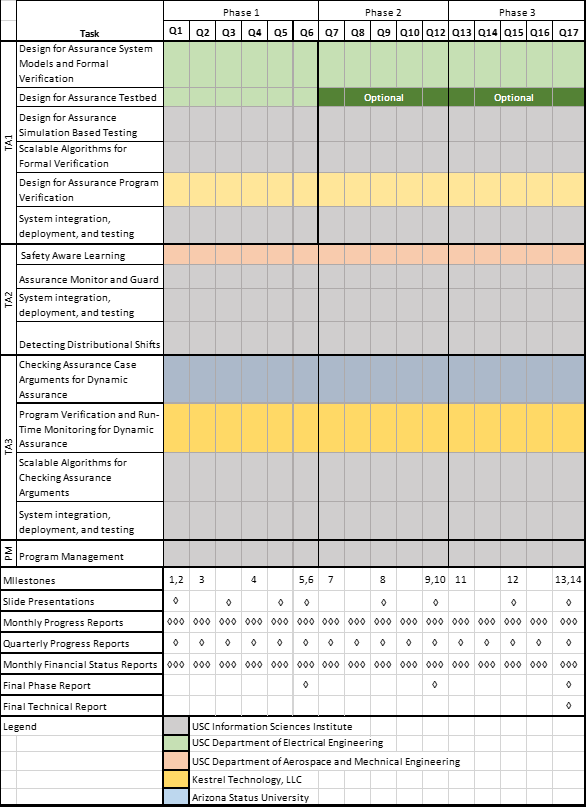
\includegraphics[width=.95\textwidth]{figs/Safeguard_Schedule_V6}
\end{center}
\vspace{-.2in}\caption{Project schedule along with a summary of milestones.  The legend maps task color to organization primary responsible for the task. } 
\label{fig:sandm}
\end{figure}
 

% \section{Level of Effort by Task \textcolor{red}{[Mike/Lisa - 1 pages]}}

% \textcolor{blue}{
% \begin{itemize}
% \item Will be a separate spreadsheet
% \item
% \end{itemize}
% }

\section*{Appendix A: Team Members and Other Information}
\addcontentsline{toc}{section}{Appendix A: Team Members and Other Information}

\baades{This section is mandatory and must include all of the following
components. If a particular subsection is not applicable, state “NONE”.}

\vspace{1ex}

\noindent
\textbf{Team Member Identification}:

\vspace{1ex}

\baades{Provide a list of all team members including the
prime, subcontractor(s), and consultant(s), as applicable. Identify specifically
whether any are a non-US organization or individual, FFRDC and/or Government
entity.}

\begin{centering}

%\small
\begin{tabular}{|p{1.8in}|p{1in}|p{1.1in}|p{0.7in}|p{0.8in}|p{0.7in}|}
\hline
 \textbf{Name} &  \textbf{Role} & \textbf{Organization} & \textbf{Non-US Org?}  & \textbf{Non-US Ind?} &  \textbf{FFRDC or Gov} \\
 \hline
Craig A. Knoblock & Prime & USC & N & N & N\\ \hline
Michael Orosz & Prime & USC & N &  N & N \\ \hline
Satish Thittamaranahalli & Prime & USC & N &  Y & N \\ \hline
Ryan Goodfellow & Prime & USC & N &  N & N \\ \hline
Anoop Kumar & Prime & USC & N & N & N \\ \hline
Satyandra Gupta & Prime & USC & N & N & N \\ \hline
Pierluigi Nuzzo & Prime & USC & N & Y & N \\ \hline
Petros Ioannou & Prime & USC & N & N & N \\ \hline
Chitta Baral & Subcontractor & ASU & N & N & N \\ \hline
Matt Barry & Subcontractor & Kestrel Technology & N & N & N \\ \hline
Douglas Smith & Subcontractor & Kestrel Technology & N & N & N \\ \hline
Henny Sipma & Subcontractor & Kestrel Technology & N & Y & N \\ \hline
\end{tabular} 
\end{centering}

\vspace{1ex}

\noindent
\textbf{Government or FFRDC Team Member Proof of Eligibility to Propose}: NONE

\baades {If
none of the team member organizations (prime or subcontractor) are a
Government entity or FFRDC, state “NONE”.}

\vspace{1ex}

\noindent
\textbf{Government or FFRDC Team Member Statement of Unique Capability}: NONE

\vspace{1ex}

\noindent
\textbf{Organizational Conflict of Interest Affirmations and Disclosure}: NONE

\vspace{1ex}

\noindent
\textbf{Intellectual Property (IP)}: 
\baades {
If no IP restrictions are intended, state “NONE”.
The Government will assume unlimited rights to all IP not explicitly identified as
having less than unlimited rights in the proposal.
For all technical data or computer software that will be furnished to the
Government with other than unlimited rights, provide (per Section VI.B.1) a list
describing all proprietary claims to results, prototypes, deliverables or systems
supporting and/or necessary for the use of the research, results, prototypes
and/or deliverables. Provide documentation proving ownership or possession of
appropriate licensing rights to all patented inventions (or inventions for which a
patent application has been filed) to be used for the proposed project.
}
\begin{centering}

%\small
\begin{tabular}{|p{2.1in}|p{1.2in}|p{1.4in}|p{2in}|}
\hline
\multicolumn{4}{|c|}{COMMERCIAL ITEMS }\\ \hline 
 \textbf{Technical Data, Computer Software To be Furnished With Restrictions} &  \textbf{Basis for Assertion} & \textbf{Asserted Rights Category} & \textbf{Name of Person Asserting Restrictions}  \\  \hline
KT Advance & Developed with mixed funding. & Restricted & David Kulich, Contracts Manager, Kestrel technology, LLC.\\ \hline
\end{tabular} 
\end{centering}

\vspace{1ex}

\noindent
\textbf{Human Subjects Research (HSR)}: NONE

\vspace{1ex}

\noindent
\textbf{Animal Use}: NONE

\vspace{1ex}

\noindent
\textbf{Representations Regarding Unpaid Delinquent Tax Liability or a Felony
Conviction under Any Federal Law}: 
%NONE

\begin{enumerate}
\item
The proposer is  not a corporation that has any unpaid Federal tax liability that has been assessed, for which all judicial and administrative remedies have been exhausted or have lapsed, and that is not being paid in a timely manner pursuant to an agreement with the authority responsible for collecting the tax liability,
\item
The proposer is not a corporation that was convicted of a felony criminal violation under a Federal law within the preceding 24 months.
\end{enumerate}

\vspace{1ex}

\noindent
\textbf{Cost Accounting Standards (CAS) Notices and Certification}:
\baades{
For any proposer who submits a proposal which, if accepted, will result in a CAS-compliant
contract, must include a Disclosure Statement as required by 48 CFR
9903.202. The disclosure forms may be found at
http://www.whitehouse.gov/omb/procurement\_casb
If this section is not applicable, state “NONE”. For further information regarding
this subject, please see www.darpa.mil/work-with-us/additional-baa.
}
NONE


%\section{Appendix B \textcolor{red}{[No Page Count]}}

\section{References}
\bibliographystyle{acm} 
\bibliography{TA3/ta3,TA2/ta2,TA1/ta1}
\end{document}
%%\documentclass[a4paper]{article}
%\documentclass[12pt]{article}
\documentclass[12pt]{dod-blank}

%% Language and font encodings
\usepackage[english]{babel}
\usepackage[utf8x]{inputenc}
\usepackage[T1]{fontenc}

%% Sets page size and margins
%%\usepackage[a4paper,top=3cm,bottom=2cm,left=3cm,right=3cm,marginparwidth=1.75cm]{geometry}
%\usepackage[top=1in, bottom=1in, left=1in, right=1in]{geometry}



%% Useful packages
\usepackage{amsmath}
\usepackage{graphicx}
  \graphicspath{{.}{./image/}}
  \DeclareGraphicsExtensions{.png,.jpg} 
\usepackage[colorinlistoftodos]{todonotes}
\usepackage[colorlinks=true, allcolors=blue]{hyperref}
\usepackage{tabularx}
\usepackage{multirow}
\usepackage{tabulary}
\usepackage{float}
\usepackage{wrapfig}
\usepackage[export]{adjustbox}
\usepackage{comment}
\usepackage{tabularx}
\usepackage{multirow}
\usepackage{tabulary}
\usepackage{enumitem}

\usepackage{listings}
\usepackage{color}
\usepackage{array}
\usepackage{subcaption}
\usepackage{xcolor}




\renewcommand{\textfraction}{0}
\renewcommand{\topfraction}{1.0}
\renewcommand{\bottomfraction}{1.0}

\usepackage{longtable}
%% macros
\newif\iffinal
\finaltrue
\iffinal
  
    \newcommand\baareq[1]{}
    \newcommand\baades[1]{}
 
 
\else
    \definecolor{darkgreen}{rgb}{0,0.4,0}
    \definecolor{darkcyan}{rgb}{0,0.4,0.4}
    \definecolor{darkblue}{rgb}{0,0,0.5}
    
    \newcommand\baareq[1]{{\color{darkcyan}[\textbf{Requirement:} #1]}}
    \newcommand\baades[1]{{\color{darkcyan}[\textbf{Description:} #1]}}
 
\fi




\def\naive{na\"{\i}ve}



\lstset{ 
  backgroundcolor=\color{white},   % choose the background color; you must add \usepackage{color} or \usepackage{xcolor}
  basicstyle=\footnotesize\ttfamily,            % the size of the fonts that are used for the code
  breakatwhitespace=false,         % sets if automatic breaks should only happen at whitespace
  breaklines=true,                 % sets automatic line breaking
  captionpos=b,                    % sets the caption-position to bottom
  commentstyle=\color{mygreen},    % comment style
  % deletekeywords={...},            % if you want to delete keywords from the given language
  escapeinside={\%*}{*)},          % if you want to add LaTeX within your code
  extendedchars=true,              % lets you use non-ASCII characters; for 8-bits encodings only, does not work with UTF-8
  frame=single,	                   % adds a frame around the code
  keepspaces=false,                 % keeps spaces in text, useful for keeping indentation of code (possibly needs columns=flexible)
  keywordstyle=\color{blue}\bfseries\underbar,       % keyword style
  language=Prolog,                 % the language of the code
  % morekeywords={if,and},        % if you want to add more keywords to the set
  numbers=none,                    % where to put the line-numbers; possible values are (none, left, right)
  numbersep=5pt,                   % how far the line-numbers are from the code
  numberstyle=\tiny\color{mygray}, % the style that is used for the line-numbers
  rulecolor=\color{black},         % if not set, the frame-color may be changed on line-breaks within not-black text
  showspaces=false,                % show spaces everywhere adding particular underscores; it overrides 'showstringspaces'
  showstringspaces=false,          % underline spaces within strings only
  showtabs=false,                  % show tabs within strings adding particular underscores
  stepnumber=2,                    % the step between two line-numbers. If it's 1, each line will be numbered
  stringstyle=\color{mymauve},     % string literal style
  tabsize=2,	                   % sets default tabsize to 2 spaces
  title=\lstname                   % show the filename of files included with \lstinputlisting; also try caption instead of title
}

% apply trick for additional keywords for our AC DSL
\lstset{
	emph={for, if, and, or},
    emphstyle={\color{blue}\bfseries\underbar}
}




\title{DARPA Assured Autonomy}
\author{Technical Volume- \textcolor{red}{Thirty-Eight (38) pages max}}

\begin{document}
\pagenumbering{roman}
 
\begin{center}
\large{\textbf{Volume 1: Technical and Management Proposal}}
\end{center}
\textbf{BAA Number:} DARPA-HR001117S0045 \\
\textbf{Technical Area:} TA1, TA2, and TA3 \\
\textbf{Proposal Title:} Assured Autonomy for Learning Enabled Vehicles (Safeguard) \\
\textbf{Lead Institution:} University of Southern California \\
\textbf{Type of organization: } “OTHER EDUCATIONAL” \\

\begin{tabularx}{\linewidth}{XX}

 \textbf{Technical Point of Contact} &  \textbf{Administrative Point of Contact }   \\
Dr.\ Craig A. Knoblock  & Sapphire Masterson  \\ 
USC Information Sciences Institute & USC Dept. of Contracts \& Grants \\
4676 Admiralty Way, Suite 1001 & 4676 Admiralty Way, Suite 1001 \\
Marina del Rey, CA 90292 & Marina del Rey, CA 90292 \\
Tel: 310-448-8786 &  Tel: (310) 448-9161 \\
E-mail: knoblock@isi.edu  & E-mail: sapphirm@usc.edu \\
\end{tabularx}
\\
\\
\textbf{Award instrument requested:}  Procurement Contract, Cost-Reimbursement, No Fee
\\
\\
\textbf{Total amount of the proposed effort:} \$ ...\\
Phase I: \$ ... \\
Phase II: \$ ... \\
Phase III: \$ ... \\
\\
\textbf{Place(s) of performance:} USC, Marina del Rey, CA; Los Angeles, CA;  Tempe, AZ; Palo Alto, CA \\
\textbf{Period(s) of performance:} 04/02/2018 - 03/31/2022     \\
\\
\textbf{Other team members:} \\
\begin{tabularx}{\linewidth}{XX}
Kestrel Technology  & Arizona State University \\
(small business) & (Other Educational)\\
POC: Matthew Barry & POC: Chitta Baral\\
3260 Hillview Avenue & Department of Computer Science and Engr. \\
Palo Alto, CA 94304 & Ira A. Fulton School of Engineering \\ 
phone: (832)205-4876 & Arizona State University\\ 
mrbarry@kestreltechnology.com & Brickyard Suite 572, 699 S. Mill Avenue \\
& Tempe, AZ 85281-8809, U.S.A.\\
& email: chitta@asu.edu\\
\end{tabularx}
\\
\textbf{Proposal validity period: } 180 days\\
\\
\textbf{Data Universal Numbering System (DUNS) number: } 072933393\\
\textbf{Taxpayer identification number:} 95-1642394\\
\textbf{Commercial and Government Entity (CAGE) code:} 1B729 Marina del Rey, CA\\
\textbf{Proposer’s reference number (if any):}  4409-0\\

\newpage
\section{Table of Contents}
\tableofcontents

\newpage
\pagenumbering{arabic}
\section{Executive Summary}
As we rapidly move into a world where machine learning plays a central role in realizing autonomous systems, it is becoming increasingly important to develop techniques that assure that these systems will operate safely and perform as expected. Current approaches are limited to providing assurance for systems with limited or no  learning capabilities. In this context, DARPA's Assured Autonomy BAA seeks to \emph{develop rigorous design and analysis technologies for continual assurance of learning-enabled autonomous systems}. USC in collaboration with Kestrel Technology and ASU is pleased to submit a comprehensive TA1, TA2, and TA3 proposal entitled \emph{``Assured Autonomy for Learning Enabled Vehicles (Safeguard).''} We plan to provide an end-to-end solution to support autonomous systems with learning-enabled components, ranging from design technologies for assurance, to assurance monitoring and control techniques, to representation and online evaluation of assurance cases. We have assembled a strong team of experts that cover the range of technologies that are required to create such an end-to-end system. If successful, the project will provide the technologies for building the next-generation of learning-enabled autonomous systems.  The entire project will take four years and cost \textcolor{red}{\$??}, with an initial version completed at the end of Phase I and successive versions with additional capabilities and improved scalability at the end of Phase II and Phase III.  

In the remainder of this section, we first introduce an  unmanned surface vehicle scenario that will be used throughout the proposal to describe the approach.  Next, we describe our approach to design, monitoring, and dynamic assurance. Finally, we introduce the team involved in the project. 

\textbf{Motivating Scenario.} Consider an autonomous unmanned surface vehicle (USV) guarding a valuable asset in the ocean when an unknown vehicle  approaches the security perimeter, under challenging weather conditions. In this scenario, the USV is required to approach the intruding vehicle, issue a warning signal, and escort it to a safe distance from the controlled area. However, as the USV has no a priori knowledge of its external environment behaviors (e.g., water depth, waves, wind, current, visibility), pre-computing a feasible trajectory, let alone optimal, becomes a non-trivial problem. For trajectory planning, the USV must continuously perform the following tasks:
\begin{itemize}[itemsep=0pt,leftmargin=*]
 \item Sense the current state of the surrounding environment (e.g., water depth, waves, wind, current, visibility) and estimate its own maneuverability constraints (e.g., braking distance, available acceleration, maximum velocity, turning radius, turning rate, safety distance) based on the state of the environment;      
\item Sense the static obstacles in the sensor range and generate a traversability map;
\item Sense the moving obstacles and classify them;   
\item Predict future trajectories of moving obstacles; 
\item Determine if any of the COLREGS \cite{commandant1999international} rules will be in effect with respect to one or more of the nearby vessels and identify the vessels with the right of way.    
\end{itemize}
The above information will be used by the trajectory planner to compute an initial trajectory, which will be continuously refined as the USV gathers additional information.
% It is not possible for the USV to be tested in every possible environment. 
The USV will use learning enabled components to take  decisions as it encounters new situations, such as  
\begin{itemize}[itemsep=0pt,leftmargin=*]
\item Classifiers to identify moving obstacles based on physical appearance and motion signatures,
\item Algorithms to estimate the sensor capabilities in adverse weather conditions,   
\item Algorithms to accurately estimate uncertainty in the environment, 
\item Classifiers to generate traversability maps,
\item Prediction of external vessel behaviors based on motion histories, 
\item Reinforcement learning  to ensure COLREGS compliance of maneuvers,  
\item Algorithms to learning pursuit behaviors.  
\end{itemize}
Learning enabled components will interact with each other in complex ways, where a misclassification error in one component may eventually compromise the entire mission.   
% We will need to make sure that each learning enabled components has a run-time monitor that will ensure that the assumptions made by the learning-enabled component remain valid and prevent erroneous learning. 
% For example, if the vehicle is exhibiting significant error in trajectory tracking, then simply downgrading the trajectory tracking error value may not be a good option.  The failure of prediction of trajectory tracking error might be due to the presence of a significant wake caused by a nearby vessel. The presence of the nearby vessel can be used to explain the degradation in trajectory tracking performance. As the vessel moves away, we can expect the trajectory tracking performance to return to the predicted level.  
While exhaustive validation of learning-enabled cyber-physical systems (LE-CPSs) is a prohibitive task~\cite{Kalra16},
their complexity, heterogeneity, and highly dynamic nature
make it challenging to even leverage existing model-based development techniques to effectively assess system correctness 
% dependability, 
at design time or enforce it at runtime.

\textbf{Design for Assurance.} Safeguard uses a platform-based design approach~\cite{Nuzzo15b} to organize the design process for a LE-CPS and to build assurance cases. Composite models are developed at several levels of abstraction,
from top-level system requirements and safety constraints down to the
implementation level.  Intermediate levels add detail to the levels
above.  The different levels are connected by refinement mappings that
allow properties established at one level to be preserved at the next
level (see Figures~\ref{fig:methodology} and~\ref{fig:assurance}).

Contracts are used to formally specify components and composite models
in terms of (1) Assumptions -- the assumed behaviors of the
environment and the behaviors of other components, and (2) Guarantees
-- the behavior properties that a model guarantees if it operates in a
context that satisfies its assumptions.  A calculus of contracts
allows horizontal composition of contracts to generate contracts for
composite models.  Vertical contracts are used to specify the mapping
or refinement relation between models at different levels of
abstraction.  The system design process starts with a high-level
contract that expresses overall system assumptions and requirements.
Subsequent levels express models with increasing detail until the
lowest level expresses the system in terms of hardware components and
their software controllers.

The assurance case for a CPS arises from the horizontal and vertical
structure of the design in several ways.  The components used within a
particular level are either (1) synthesized using
correct-by-construction design tools together with proofs, (2) derived
statically or dynamically using safety-aware machine-learning
techniques, (3) written manually and verified by analysis tools, or
(4) written manually and validated by extensive testing.  The
assurance case for the whole reflects its compositional structure.  We
anticipate that well-specified contracts together with the calculus of
contracts will eliminate well-known problems with unexpected emergent
behaviors in CPS systems.

The assurance case for the lowest-layer design arises from both the
intra-level assurance and from properties and their proofs that are
preserved under the refinement mapping from the top-level
requirements.  The refinement mappings between model layers will be
constructed using a variety of techniques.  A contract at an abstract
level can be mapped to a component or refined contract by (1)
retrieval of pre-verified components from a platform library, (2)
synthesis using correct-by-construction design and optimization tools,
or (3) manual coding to satisfy a contract.  The mapping of a
composite model will be composed from the mappings of its constituent
components or contracts.  When a composite model cannot be mapped
compositionally to the next level, it will be generated using
correct-by-construction design and optimization tools.

\textbf{Assurance Monitoring and Control.}
We provide an integrated framework for safety-aware learning, assurance monitoring and control, detecting distribution shifts. Three major components offer an efficient TA2 architecture as well as interfaces with TA1 and TA3, that is, (a) safety-aware learning and planning, (b) assurance monitors for guarding architectural and safety constraints; and (c) distribution shift detection.

We will develop a new learning-enabled online decision-making framework that allows opportunistically composing a sequence of actions (maneuvers) to reduce uncertainty in the system capability model without suspending the progress toward the mission goals or compromising safety. Each candidate action is evaluated based on three criteria: (1) the risk of violating a safety constraint using the current uncertainties in the parameter estimates; (2) its relevance to the mission goals; (3)  its expected information gain, i.e., reduction in uncertainty, with respect to the parameter estimates. These evaluations are combined to produce a cumulative mission utility value for each action that drives our learning-enabled decision-making framework. The problem of generating and evaluating sequences of actions can be posed in several way. For example, it can be solved using a branch-and-bound search method like Anytime A*, or formulated with the finite-horizon Markov Decision Process (MDP) framework. We will develop new scalable search strategies to solve this problem efficiently, by potentially evaluating a recent method developed at USC, called FastMap, that can significantly improve the execution time. 

We will develop monitors for architectural and safety constraints. 
% While these constraints can be checked over and over again as sensor information flow in, this naive strategy accounts for a lot of computational overhead. 
To achieve scalability and decrease the overhead, we propose the application of a technique that we currently use in DARPA's RSPACE program, which leverages a physical model of the vehicles dynamics and its interactions with the environment to efficiently determine the readout frequency. We propose two  extensions of this basic idea. First, we will use the theory of Variable Elimination to prioritize which variables to monitor, e.g., controllable, versus uncontrollable, adversarially controlled, or unobservable variables. Second, we invoke the dynamic assessment of assurance cases only when needed. This  decreases the number of times dynamic assessment of assurance cases is initiated as well as the communication bandwidth between the TA2 and TA3 components.

Finally, we will identify a distribution shift by combining statistical and machine learning techniques to differentiate between environmental and sensor changes. We will exploit a categorization of the shifts based on their cause and duration as well as extend our earlier work on detecting and mitigating sensor failures for all types of monitored variables.  

\textbf{Dynamic Assurance:} The Safeguard {\em design for assurance\/} activity takes a systems-theoretic stance toward safety.  Consequently, it presumes that safety is an emergent property of the system, and that hazards can present themselves through unintended interactions and performance violations in addition to causal events such as component failures.  Our design approach includes consideration of intent as well as hazard analysis and mitigation.  The artifacts from these activities populate contracts and assumptions for the dynamic assurance case.  
We thus build safety into the product by working at a systems-level viewpoint, using lexicon and design patterns familiar to both hardware and software engineers; safety is an emergent property of the system, not an afterthought.  
As system behavior evolves during runtime owing to learning, threats, degradation, or some other factor, the dynamic assurance case identifies whether the safety constraints continue to be satisfied.  If not, it provides notifications or issues recovery instructions directly from a lookup table.

Our implementation of the dynamic assurance case employs a declarative knowledge base inference engine and a domain-specific language tailored to our approach.  We have used them successfully for assurance case tool sets and arguments, and will extend them to reason about uncertainty and learning.  Our approach to achieve scalability is to specialize solvers toward modularity and to take advantage of domain knowledge.  Specifically, we will develop answer set programming techniques for context-dependent learning for reasoning about the learning-enabled components as well as learning assurance rules.  We will develop new formalisms for uncertainty to include causality, using weights for computing probabilities, and probabilistic non-monotonicity.  To achieve scaling objectives we will implement specializations using modularity, weighted CSPs, and message passing. 

% The system safety constraints revealed from that design become the key elements of our dynamic assurance case.  Our verification tools ensure the constraints are relevant, identifiable, and their implementation and effect observable.  

\textbf{Team.} We have assembled a team that is exceptionally well-qualified to build the proposed Safeguard system.  The team will be led by Dr.\ Craig Knoblock, the Principal Investigator for the effort, who currently leads the Intelligent Systems Division at the Information Sciences Institute.  He has led many large DARPA and IARPA projects over the years and has a strong track record in conducting leading edge research and then transitioning the technology to commercial use.  He will be supported by Dr.\ Michael Orosz as the Project Manager, who also has  experience in managing large research projects and on autonomous systems.  The TA1 team will be led by Dr.\ Pierluigi Nuzzo, who is an expert in embedded system design methodologies and the  application of formal methods to cyber-physical systems.  The TA1 team also includes Dr.\ Doug Smith, who has spent many years working on scalable correct-by-construction techniques and Dr.\ Henny Sipma, who has significant experience in applying program verification methods to real-world problems.  The TA1 team also includes Ryan Goodfellow, who has done a large amount of work on simulation-based testing.  The TA2 team will be led by Dr.\ Knoblock who has worked on topics related to both monitoring and detecting distribution changes.  He will be supported by Dr.\ Satyandra Gupta, who is an expert on autonomous surface vehicles as well as on safety-aware learning. He will also be supported by Drs.\ Anoop Kumar and Satish Thittamaranahalli, who have also previously worked on efficient methods for execution monitoring.  The TA3 team will be lead by Dr.\ Matthew Barry, who has experience in creating the technologies for assurance cases.  He will be supported by Dr.\ Chitta Baral, who is an expert on ASP solvers and by Dr.\ Thittamaranahalli who is an expert on SAT solvers, both of which will be applied to provide scalable assurance case reasoning.  Finally, Dr.\ Petros Ioannou, who is an expert on control systems for autonomous vehicles will provide an autonomous vehicle platform, which will form the focus of our work until the TA4 teams provide additional vehicle platforms for development.  

\newpage
\section{Innovative Claims and Deliverables}

In this project we will develop and build an end-to-end system for assured autonomy.  This section describes the key innovations by technical area and then the overall deliverables of the project.

\paragraph{Design for Assurance}

\begin{itemize}[itemsep=0pt,leftmargin=*]
\item We address the LE-CPS design challenges via a holistic approach that can contextually generate design artifacts and assurance cases. We develop a compositional, contract-based modeling framework, methods, and tools to support the design process from system-level requirement capture,  formalization, and analysis, to the generation, testing, and continual monitoring of software and hardware artifacts in feedback loop with a physical process.

\item We develop compositional abstractions and interfaces (vertical contracts) that can  bridge heterogeneous formalisms and heterogeneous decomposition architectures to make system analysis and synthesis tractable, consistently combine different verification and synthesis methods at design time, and provide seamless support for dynamic assurance at run time. %We aim to quantitatively capture the confidence in the satisfaction of requirements under uncertain or unknown conditions, and resilience properties of  systems at different abstraction levels, to enable trade-off evaluation between resilience, performance, and cost.

\item We develop a unifying framework and efficient algorithms to reason about the combination of discrete and continuous dynamics and constraints in the presence of uncertainties in LE-CPS using a satisfiability modulo convex approach~\cite{Shoukry2017} for contract-based system verification and scalable trajectory planning.  

\item We provide an environment for high-fidelity CPS testing, in which production-ready software, e.g.,  safety-critical learning and control, may be deployed and tested 
% by extending the Cypress testbed environment \cite{Goodfellow2015Cypress:Systems} 
with time dilation facilities, so that it synchronizes with a physical simulation that is not necessarily running in real time, while still having the perception of real time.

\item We 
% These facilities allow a cyber system to be  
propose an approach for unanticipated behavior space identification and test coverage maximization which leverages results from the theory of differential algebraic equation (DAE)~\cite{Berger2013ControllabilitySurvey,Ilchmann2005ATheory,BergerOnSystems,Lamour2013} 
to prune the behavior search space and identify smaller regions of interest for efficient simulation-based testing. 
% We then compute the intersection of these two behavior spaces and restrict our simulation based testing search space to this subspace.
\end{itemize}

\paragraph{Assurance Monitoring and Control}

\begin{itemize}[itemsep=0pt,leftmargin=*]
\item 
%We integrate safety-aware learning into the overall decision making problem. The goal is to maximize mission utility without violating the safety constraints. 
Our safety-aware learning framework enables the system to opportunistically select and execute actions to assist the learning-enabled component in reducing model uncertainty without compromising safety or deviating from the mission goals. The value of uncertainty reduction is explicitly incorporated in the optimization process for selecting the best action.  
\item For safety-aware learning, we propose the idea of preprocessing the search space of the problem domain before queries and observations come in. With such a linear-time preprocessing phase, the performance of search and optimization algorithms can be significantly boosted. For example, in regular A* search, the intensional or extensional search space can be preprocessed in near-linear time to yield an embedding of each state as a point in Euclidean space~\cite{cujakk}. Then, when the query comes in, A* search can make use of these Euclidean distances as heuristic distances between two states to yield order-of-magnitude speedups. 
%In Anytime A* for safety-aware learning and planning, this leads to a significantly better quality of actions chosen within a time limit, and in the MDP framework, the same ideas can be used to improve the convergence of Bellman updates for safety-aware Reinforcement Learning.
\item As massive amounts of sensor information flow in, it is imperative for us to efficiently process this information for monitoring architectural and safety constraints. Building on our past work on similar tasks, we propose novel technologies for efficiently monitoring constraints. These algorithms can yield an exponential reduction in the amount of sensor data that needs to be processed. Doing this also reduces the message complexities between the various modules. %We also propose to use the theory of Variable Elimination (VE) to monitor constraints with uncontrollable, adversarially controlled, and/or unobservable variables. VE yields a substrate constraint to monitor that characterizes a dominant strategy of the controllable variables over the uncontrollable, adversarially controlled, and/or unobservable variables.
\item We will develop techniques to identify  distributional shifts and determine the underlying cause (e.g., change in environment, sensor failure,   etc.), as well as strategies for handling the various distributional shifts.   Notably, we propose to build on our past work and use compact representations to exploit historical data to identify distributional shifts.
\end{itemize}

\paragraph{Dynamic Assurance}

\begin{itemize}[itemsep=0pt,leftmargin=*]

\item We demonstrate the integration of dynamic assurance for safety-critical learning-enabled dynamic systems in which evolutionary behaviors are expected and tolerated as a property of the functionality.   The impact will be consequential contributions safety-critical dynamic systems in which evolutionary behaviors are expected and tolerated as portion of the functionality.   
\item We implement dynamic assurance by combining features of system safety, formal methods, logic programming, uncertain reasoning, and domain-specific languages.  We populate assurance case arguments at several levels of modeling and implementation abstraction, using the analysis results to produce design-time evidence supporting assurance claims.  
%We provide automated reasoning about the assurance case itself to produce verification, consistency, and completeness results for the argument.  Dynamic assurance results then yield trusted explanations of whether safety constraints and assumptions and other contracts still hold during the collection of runtime evidence from monitors. 
\item We develop and demonstrate ASP formalisms crucial to applications in dynamic assurance. We demonstrate the suitability of the technology especially for assurance case arguments owing to the improved legibility, consistency and completeness checks, handling of uncertain and default reasoning, and scalability.  
%We will produce modularized solvers for enhanced performance based on recent algorithmic developments in exploiting structure, kernelization, and message passing. We provide a formalism to enable learning of assurance rules. 
We provide a novel approach to handling uncertainty that provides the ability to do causal and counter-factual reasoning as well as probabilistic non-monotonicity.  Overcoming limitations of traditional inductive logic techniques, we develop a novel iterative and incremental approach based on context dependent learning. 
\end{itemize}

\paragraph{Deliverables}
During the course of this project, we will build and deliver a fully-operational system that covers all three of the technical areas.  The detailed capabilities of this system are described in the individual technical sections.  The resulting system will be available as open source under a permissive license, which will allow other organizations to use the work, extend it in new directions, and even commercialize the software.  Kestrel Technology has significant experience in this space and has built and applied these types of technologies to a variety of real world tasks.  Kestrel is ideally suited to pursue commercial uses of this technology and the permissive license will facilitate exploring these opportunities since there will be no need to negotiate intellectual property rights.  

\newpage
\section{Technical Plan}
%%\documentclass[a4paper]{article}
%\documentclass[12pt]{article}
\documentclass[12pt]{dod-blank}

%% Language and font encodings
\usepackage[english]{babel}
\usepackage[utf8x]{inputenc}
\usepackage[T1]{fontenc}

%% Sets page size and margins
%%\usepackage[a4paper,top=3cm,bottom=2cm,left=3cm,right=3cm,marginparwidth=1.75cm]{geometry}
%\usepackage[top=1in, bottom=1in, left=1in, right=1in]{geometry}



%% Useful packages
\usepackage{amsmath}
\usepackage{graphicx}
  \graphicspath{{.}{./image/}}
  \DeclareGraphicsExtensions{.png,.jpg} 
\usepackage[colorinlistoftodos]{todonotes}
\usepackage[colorlinks=true, allcolors=blue]{hyperref}
\usepackage{tabularx}
\usepackage{multirow}
\usepackage{tabulary}
\usepackage{float}
\usepackage{wrapfig}
\usepackage[export]{adjustbox}
\usepackage{comment}
\usepackage{tabularx}
\usepackage{multirow}
\usepackage{tabulary}
\usepackage{enumitem}

\usepackage{listings}
\usepackage{color}
\usepackage{array}
\usepackage{subcaption}
\usepackage{xcolor}




\renewcommand{\textfraction}{0}
\renewcommand{\topfraction}{1.0}
\renewcommand{\bottomfraction}{1.0}

\usepackage{longtable}
%% macros
\newif\iffinal
\finaltrue
\iffinal
  
    \newcommand\baareq[1]{}
    \newcommand\baades[1]{}
 
 
\else
    \definecolor{darkgreen}{rgb}{0,0.4,0}
    \definecolor{darkcyan}{rgb}{0,0.4,0.4}
    \definecolor{darkblue}{rgb}{0,0,0.5}
    
    \newcommand\baareq[1]{{\color{darkcyan}[\textbf{Requirement:} #1]}}
    \newcommand\baades[1]{{\color{darkcyan}[\textbf{Description:} #1]}}
 
\fi




\def\naive{na\"{\i}ve}



\lstset{ 
  backgroundcolor=\color{white},   % choose the background color; you must add \usepackage{color} or \usepackage{xcolor}
  basicstyle=\footnotesize\ttfamily,            % the size of the fonts that are used for the code
  breakatwhitespace=false,         % sets if automatic breaks should only happen at whitespace
  breaklines=true,                 % sets automatic line breaking
  captionpos=b,                    % sets the caption-position to bottom
  commentstyle=\color{mygreen},    % comment style
  % deletekeywords={...},            % if you want to delete keywords from the given language
  escapeinside={\%*}{*)},          % if you want to add LaTeX within your code
  extendedchars=true,              % lets you use non-ASCII characters; for 8-bits encodings only, does not work with UTF-8
  frame=single,	                   % adds a frame around the code
  keepspaces=false,                 % keeps spaces in text, useful for keeping indentation of code (possibly needs columns=flexible)
  keywordstyle=\color{blue}\bfseries\underbar,       % keyword style
  language=Prolog,                 % the language of the code
  % morekeywords={if,and},        % if you want to add more keywords to the set
  numbers=none,                    % where to put the line-numbers; possible values are (none, left, right)
  numbersep=5pt,                   % how far the line-numbers are from the code
  numberstyle=\tiny\color{mygray}, % the style that is used for the line-numbers
  rulecolor=\color{black},         % if not set, the frame-color may be changed on line-breaks within not-black text
  showspaces=false,                % show spaces everywhere adding particular underscores; it overrides 'showstringspaces'
  showstringspaces=false,          % underline spaces within strings only
  showtabs=false,                  % show tabs within strings adding particular underscores
  stepnumber=2,                    % the step between two line-numbers. If it's 1, each line will be numbered
  stringstyle=\color{mymauve},     % string literal style
  tabsize=2,	                   % sets default tabsize to 2 spaces
  title=\lstname                   % show the filename of files included with \lstinputlisting; also try caption instead of title
}

% apply trick for additional keywords for our AC DSL
\lstset{
	emph={for, if, and, or},
    emphstyle={\color{blue}\bfseries\underbar}
}




\title{DARPA Assured Autonomy}
\author{Technical Volume- \textcolor{red}{Thirty-Eight (38) pages max}}

\begin{document}
\pagenumbering{roman}
\include{cover}

\newpage
\section{Table of Contents}
\tableofcontents

\newpage
\pagenumbering{arabic}
\section{Executive Summary}
As we rapidly move into a world where machine learning plays a central role in realizing autonomous systems, it is becoming increasingly important to develop techniques that assure that these systems will operate safely and perform as expected. Current approaches are limited to providing assurance for systems with limited or no  learning capabilities. In this context, DARPA's Assured Autonomy BAA seeks to \emph{develop rigorous design and analysis technologies for continual assurance of learning-enabled autonomous systems}. USC in collaboration with Kestrel Technology and ASU is pleased to submit a comprehensive TA1, TA2, and TA3 proposal entitled \emph{``Assured Autonomy for Learning Enabled Vehicles (Safeguard).''} We plan to provide an end-to-end solution to support autonomous systems with learning-enabled components, ranging from design technologies for assurance, to assurance monitoring and control techniques, to representation and online evaluation of assurance cases. We have assembled a strong team of experts that cover the range of technologies that are required to create such an end-to-end system. If successful, the project will provide the technologies for building the next-generation of learning-enabled autonomous systems.  The entire project will take four years and cost \textcolor{red}{\$??}, with an initial version completed at the end of Phase I and successive versions with additional capabilities and improved scalability at the end of Phase II and Phase III.  

In the remainder of this section, we first introduce an  unmanned surface vehicle scenario that will be used throughout the proposal to describe the approach.  Next, we describe our approach to design, monitoring, and dynamic assurance. Finally, we introduce the team involved in the project. 

\textbf{Motivating Scenario.} Consider an autonomous unmanned surface vehicle (USV) guarding a valuable asset in the ocean when an unknown vehicle  approaches the security perimeter, under challenging weather conditions. In this scenario, the USV is required to approach the intruding vehicle, issue a warning signal, and escort it to a safe distance from the controlled area. However, as the USV has no a priori knowledge of its external environment behaviors (e.g., water depth, waves, wind, current, visibility), pre-computing a feasible trajectory, let alone optimal, becomes a non-trivial problem. For trajectory planning, the USV must continuously perform the following tasks:
\begin{itemize}[itemsep=0pt,leftmargin=*]
 \item Sense the current state of the surrounding environment (e.g., water depth, waves, wind, current, visibility) and estimate its own maneuverability constraints (e.g., braking distance, available acceleration, maximum velocity, turning radius, turning rate, safety distance) based on the state of the environment;      
\item Sense the static obstacles in the sensor range and generate a traversability map;
\item Sense the moving obstacles and classify them;   
\item Predict future trajectories of moving obstacles; 
\item Determine if any of the COLREGS \cite{commandant1999international} rules will be in effect with respect to one or more of the nearby vessels and identify the vessels with the right of way.    
\end{itemize}
The above information will be used by the trajectory planner to compute an initial trajectory, which will be continuously refined as the USV gathers additional information.
% It is not possible for the USV to be tested in every possible environment. 
The USV will use learning enabled components to take  decisions as it encounters new situations, such as  
\begin{itemize}[itemsep=0pt,leftmargin=*]
\item Classifiers to identify moving obstacles based on physical appearance and motion signatures,
\item Algorithms to estimate the sensor capabilities in adverse weather conditions,   
\item Algorithms to accurately estimate uncertainty in the environment, 
\item Classifiers to generate traversability maps,
\item Prediction of external vessel behaviors based on motion histories, 
\item Reinforcement learning  to ensure COLREGS compliance of maneuvers,  
\item Algorithms to learning pursuit behaviors.  
\end{itemize}
Learning enabled components will interact with each other in complex ways, where a misclassification error in one component may eventually compromise the entire mission.   
% We will need to make sure that each learning enabled components has a run-time monitor that will ensure that the assumptions made by the learning-enabled component remain valid and prevent erroneous learning. 
% For example, if the vehicle is exhibiting significant error in trajectory tracking, then simply downgrading the trajectory tracking error value may not be a good option.  The failure of prediction of trajectory tracking error might be due to the presence of a significant wake caused by a nearby vessel. The presence of the nearby vessel can be used to explain the degradation in trajectory tracking performance. As the vessel moves away, we can expect the trajectory tracking performance to return to the predicted level.  
While exhaustive validation of learning-enabled cyber-physical systems (LE-CPSs) is a prohibitive task~\cite{Kalra16},
their complexity, heterogeneity, and highly dynamic nature
make it challenging to even leverage existing model-based development techniques to effectively assess system correctness 
% dependability, 
at design time or enforce it at runtime.

\textbf{Design for Assurance.} Safeguard uses a platform-based design approach~\cite{Nuzzo15b} to organize the design process for a LE-CPS and to build assurance cases. Composite models are developed at several levels of abstraction,
from top-level system requirements and safety constraints down to the
implementation level.  Intermediate levels add detail to the levels
above.  The different levels are connected by refinement mappings that
allow properties established at one level to be preserved at the next
level (see Figures~\ref{fig:methodology} and~\ref{fig:assurance}).

Contracts are used to formally specify components and composite models
in terms of (1) Assumptions -- the assumed behaviors of the
environment and the behaviors of other components, and (2) Guarantees
-- the behavior properties that a model guarantees if it operates in a
context that satisfies its assumptions.  A calculus of contracts
allows horizontal composition of contracts to generate contracts for
composite models.  Vertical contracts are used to specify the mapping
or refinement relation between models at different levels of
abstraction.  The system design process starts with a high-level
contract that expresses overall system assumptions and requirements.
Subsequent levels express models with increasing detail until the
lowest level expresses the system in terms of hardware components and
their software controllers.

The assurance case for a CPS arises from the horizontal and vertical
structure of the design in several ways.  The components used within a
particular level are either (1) synthesized using
correct-by-construction design tools together with proofs, (2) derived
statically or dynamically using safety-aware machine-learning
techniques, (3) written manually and verified by analysis tools, or
(4) written manually and validated by extensive testing.  The
assurance case for the whole reflects its compositional structure.  We
anticipate that well-specified contracts together with the calculus of
contracts will eliminate well-known problems with unexpected emergent
behaviors in CPS systems.

The assurance case for the lowest-layer design arises from both the
intra-level assurance and from properties and their proofs that are
preserved under the refinement mapping from the top-level
requirements.  The refinement mappings between model layers will be
constructed using a variety of techniques.  A contract at an abstract
level can be mapped to a component or refined contract by (1)
retrieval of pre-verified components from a platform library, (2)
synthesis using correct-by-construction design and optimization tools,
or (3) manual coding to satisfy a contract.  The mapping of a
composite model will be composed from the mappings of its constituent
components or contracts.  When a composite model cannot be mapped
compositionally to the next level, it will be generated using
correct-by-construction design and optimization tools.

\textbf{Assurance Monitoring and Control.}
We provide an integrated framework for safety-aware learning, assurance monitoring and control, detecting distribution shifts. Three major components offer an efficient TA2 architecture as well as interfaces with TA1 and TA3, that is, (a) safety-aware learning and planning, (b) assurance monitors for guarding architectural and safety constraints; and (c) distribution shift detection.

We will develop a new learning-enabled online decision-making framework that allows opportunistically composing a sequence of actions (maneuvers) to reduce uncertainty in the system capability model without suspending the progress toward the mission goals or compromising safety. Each candidate action is evaluated based on three criteria: (1) the risk of violating a safety constraint using the current uncertainties in the parameter estimates; (2) its relevance to the mission goals; (3)  its expected information gain, i.e., reduction in uncertainty, with respect to the parameter estimates. These evaluations are combined to produce a cumulative mission utility value for each action that drives our learning-enabled decision-making framework. The problem of generating and evaluating sequences of actions can be posed in several way. For example, it can be solved using a branch-and-bound search method like Anytime A*, or formulated with the finite-horizon Markov Decision Process (MDP) framework. We will develop new scalable search strategies to solve this problem efficiently, by potentially evaluating a recent method developed at USC, called FastMap, that can significantly improve the execution time. 

We will develop monitors for architectural and safety constraints. 
% While these constraints can be checked over and over again as sensor information flow in, this naive strategy accounts for a lot of computational overhead. 
To achieve scalability and decrease the overhead, we propose the application of a technique that we currently use in DARPA's RSPACE program, which leverages a physical model of the vehicles dynamics and its interactions with the environment to efficiently determine the readout frequency. We propose two  extensions of this basic idea. First, we will use the theory of Variable Elimination to prioritize which variables to monitor, e.g., controllable, versus uncontrollable, adversarially controlled, or unobservable variables. Second, we invoke the dynamic assessment of assurance cases only when needed. This  decreases the number of times dynamic assessment of assurance cases is initiated as well as the communication bandwidth between the TA2 and TA3 components.

Finally, we will identify a distribution shift by combining statistical and machine learning techniques to differentiate between environmental and sensor changes. We will exploit a categorization of the shifts based on their cause and duration as well as extend our earlier work on detecting and mitigating sensor failures for all types of monitored variables.  

\textbf{Dynamic Assurance:} The Safeguard {\em design for assurance\/} activity takes a systems-theoretic stance toward safety.  Consequently, it presumes that safety is an emergent property of the system, and that hazards can present themselves through unintended interactions and performance violations in addition to causal events such as component failures.  Our design approach includes consideration of intent as well as hazard analysis and mitigation.  The artifacts from these activities populate contracts and assumptions for the dynamic assurance case.  
We thus build safety into the product by working at a systems-level viewpoint, using lexicon and design patterns familiar to both hardware and software engineers; safety is an emergent property of the system, not an afterthought.  
As system behavior evolves during runtime owing to learning, threats, degradation, or some other factor, the dynamic assurance case identifies whether the safety constraints continue to be satisfied.  If not, it provides notifications or issues recovery instructions directly from a lookup table.

Our implementation of the dynamic assurance case employs a declarative knowledge base inference engine and a domain-specific language tailored to our approach.  We have used them successfully for assurance case tool sets and arguments, and will extend them to reason about uncertainty and learning.  Our approach to achieve scalability is to specialize solvers toward modularity and to take advantage of domain knowledge.  Specifically, we will develop answer set programming techniques for context-dependent learning for reasoning about the learning-enabled components as well as learning assurance rules.  We will develop new formalisms for uncertainty to include causality, using weights for computing probabilities, and probabilistic non-monotonicity.  To achieve scaling objectives we will implement specializations using modularity, weighted CSPs, and message passing. 

% The system safety constraints revealed from that design become the key elements of our dynamic assurance case.  Our verification tools ensure the constraints are relevant, identifiable, and their implementation and effect observable.  

\textbf{Team.} We have assembled a team that is exceptionally well-qualified to build the proposed Safeguard system.  The team will be led by Dr.\ Craig Knoblock, the Principal Investigator for the effort, who currently leads the Intelligent Systems Division at the Information Sciences Institute.  He has led many large DARPA and IARPA projects over the years and has a strong track record in conducting leading edge research and then transitioning the technology to commercial use.  He will be supported by Dr.\ Michael Orosz as the Project Manager, who also has  experience in managing large research projects and on autonomous systems.  The TA1 team will be led by Dr.\ Pierluigi Nuzzo, who is an expert in embedded system design methodologies and the  application of formal methods to cyber-physical systems.  The TA1 team also includes Dr.\ Doug Smith, who has spent many years working on scalable correct-by-construction techniques and Dr.\ Henny Sipma, who has significant experience in applying program verification methods to real-world problems.  The TA1 team also includes Ryan Goodfellow, who has done a large amount of work on simulation-based testing.  The TA2 team will be led by Dr.\ Knoblock who has worked on topics related to both monitoring and detecting distribution changes.  He will be supported by Dr.\ Satyandra Gupta, who is an expert on autonomous surface vehicles as well as on safety-aware learning. He will also be supported by Drs.\ Anoop Kumar and Satish Thittamaranahalli, who have also previously worked on efficient methods for execution monitoring.  The TA3 team will be lead by Dr.\ Matthew Barry, who has experience in creating the technologies for assurance cases.  He will be supported by Dr.\ Chitta Baral, who is an expert on ASP solvers and by Dr.\ Thittamaranahalli who is an expert on SAT solvers, both of which will be applied to provide scalable assurance case reasoning.  Finally, Dr.\ Petros Ioannou, who is an expert on control systems for autonomous vehicles will provide an autonomous vehicle platform, which will form the focus of our work until the TA4 teams provide additional vehicle platforms for development.  

\newpage
\section{Innovative Claims and Deliverables}

In this project we will develop and build an end-to-end system for assured autonomy.  This section describes the key innovations by technical area and then the overall deliverables of the project.

\paragraph{Design for Assurance}

\begin{itemize}[itemsep=0pt,leftmargin=*]
\item We address the LE-CPS design challenges via a holistic approach that can contextually generate design artifacts and assurance cases. We develop a compositional, contract-based modeling framework, methods, and tools to support the design process from system-level requirement capture,  formalization, and analysis, to the generation, testing, and continual monitoring of software and hardware artifacts in feedback loop with a physical process.

\item We develop compositional abstractions and interfaces (vertical contracts) that can  bridge heterogeneous formalisms and heterogeneous decomposition architectures to make system analysis and synthesis tractable, consistently combine different verification and synthesis methods at design time, and provide seamless support for dynamic assurance at run time. %We aim to quantitatively capture the confidence in the satisfaction of requirements under uncertain or unknown conditions, and resilience properties of  systems at different abstraction levels, to enable trade-off evaluation between resilience, performance, and cost.

\item We develop a unifying framework and efficient algorithms to reason about the combination of discrete and continuous dynamics and constraints in the presence of uncertainties in LE-CPS using a satisfiability modulo convex approach~\cite{Shoukry2017} for contract-based system verification and scalable trajectory planning.  

\item We provide an environment for high-fidelity CPS testing, in which production-ready software, e.g.,  safety-critical learning and control, may be deployed and tested 
% by extending the Cypress testbed environment \cite{Goodfellow2015Cypress:Systems} 
with time dilation facilities, so that it synchronizes with a physical simulation that is not necessarily running in real time, while still having the perception of real time.

\item We 
% These facilities allow a cyber system to be  
propose an approach for unanticipated behavior space identification and test coverage maximization which leverages results from the theory of differential algebraic equation (DAE)~\cite{Berger2013ControllabilitySurvey,Ilchmann2005ATheory,BergerOnSystems,Lamour2013} 
to prune the behavior search space and identify smaller regions of interest for efficient simulation-based testing. 
% We then compute the intersection of these two behavior spaces and restrict our simulation based testing search space to this subspace.
\end{itemize}

\paragraph{Assurance Monitoring and Control}

\begin{itemize}[itemsep=0pt,leftmargin=*]
\item 
%We integrate safety-aware learning into the overall decision making problem. The goal is to maximize mission utility without violating the safety constraints. 
Our safety-aware learning framework enables the system to opportunistically select and execute actions to assist the learning-enabled component in reducing model uncertainty without compromising safety or deviating from the mission goals. The value of uncertainty reduction is explicitly incorporated in the optimization process for selecting the best action.  
\item For safety-aware learning, we propose the idea of preprocessing the search space of the problem domain before queries and observations come in. With such a linear-time preprocessing phase, the performance of search and optimization algorithms can be significantly boosted. For example, in regular A* search, the intensional or extensional search space can be preprocessed in near-linear time to yield an embedding of each state as a point in Euclidean space~\cite{cujakk}. Then, when the query comes in, A* search can make use of these Euclidean distances as heuristic distances between two states to yield order-of-magnitude speedups. 
%In Anytime A* for safety-aware learning and planning, this leads to a significantly better quality of actions chosen within a time limit, and in the MDP framework, the same ideas can be used to improve the convergence of Bellman updates for safety-aware Reinforcement Learning.
\item As massive amounts of sensor information flow in, it is imperative for us to efficiently process this information for monitoring architectural and safety constraints. Building on our past work on similar tasks, we propose novel technologies for efficiently monitoring constraints. These algorithms can yield an exponential reduction in the amount of sensor data that needs to be processed. Doing this also reduces the message complexities between the various modules. %We also propose to use the theory of Variable Elimination (VE) to monitor constraints with uncontrollable, adversarially controlled, and/or unobservable variables. VE yields a substrate constraint to monitor that characterizes a dominant strategy of the controllable variables over the uncontrollable, adversarially controlled, and/or unobservable variables.
\item We will develop techniques to identify  distributional shifts and determine the underlying cause (e.g., change in environment, sensor failure,   etc.), as well as strategies for handling the various distributional shifts.   Notably, we propose to build on our past work and use compact representations to exploit historical data to identify distributional shifts.
\end{itemize}

\paragraph{Dynamic Assurance}

\begin{itemize}[itemsep=0pt,leftmargin=*]

\item We demonstrate the integration of dynamic assurance for safety-critical learning-enabled dynamic systems in which evolutionary behaviors are expected and tolerated as a property of the functionality.   The impact will be consequential contributions safety-critical dynamic systems in which evolutionary behaviors are expected and tolerated as portion of the functionality.   
\item We implement dynamic assurance by combining features of system safety, formal methods, logic programming, uncertain reasoning, and domain-specific languages.  We populate assurance case arguments at several levels of modeling and implementation abstraction, using the analysis results to produce design-time evidence supporting assurance claims.  
%We provide automated reasoning about the assurance case itself to produce verification, consistency, and completeness results for the argument.  Dynamic assurance results then yield trusted explanations of whether safety constraints and assumptions and other contracts still hold during the collection of runtime evidence from monitors. 
\item We develop and demonstrate ASP formalisms crucial to applications in dynamic assurance. We demonstrate the suitability of the technology especially for assurance case arguments owing to the improved legibility, consistency and completeness checks, handling of uncertain and default reasoning, and scalability.  
%We will produce modularized solvers for enhanced performance based on recent algorithmic developments in exploiting structure, kernelization, and message passing. We provide a formalism to enable learning of assurance rules. 
We provide a novel approach to handling uncertainty that provides the ability to do causal and counter-factual reasoning as well as probabilistic non-monotonicity.  Overcoming limitations of traditional inductive logic techniques, we develop a novel iterative and incremental approach based on context dependent learning. 
\end{itemize}

\paragraph{Deliverables}
During the course of this project, we will build and deliver a fully-operational system that covers all three of the technical areas.  The detailed capabilities of this system are described in the individual technical sections.  The resulting system will be available as open source under a permissive license, which will allow other organizations to use the work, extend it in new directions, and even commercialize the software.  Kestrel Technology has significant experience in this space and has built and applied these types of technologies to a variety of real world tasks.  Kestrel is ideally suited to pursue commercial uses of this technology and the permissive license will facilitate exploring these opportunities since there will be no need to negotiate intellectual property rights.  

\newpage
\section{Technical Plan}
\input{./TA1/main}
\input{./TA2/main}
\input{./TA3/main}
\clearpage
\newpage


\section{Management Plan}


The Principal Investigator for this effort is Dr. Craig Knoblock who is responsible for all aspects of the effort, will coordinate the parallel team efforts, and will ensure high levels of performance from individual team members.  The Co-P/I, Dr. Michael Orosz, will provide project management and will assist all performers in the execution of the project.    The project team is divided into three working groups (Figure~\ref{fig:org_chart}) corresponding to Technical Areas 1-3, however, members of each team contribute across all project activities.   Table~\ref{fig:Table_Mgmt} defines the major contributions of each project team member to the project tasks.

\begin{figure}[tbhp]
%\vspace{-25pt}
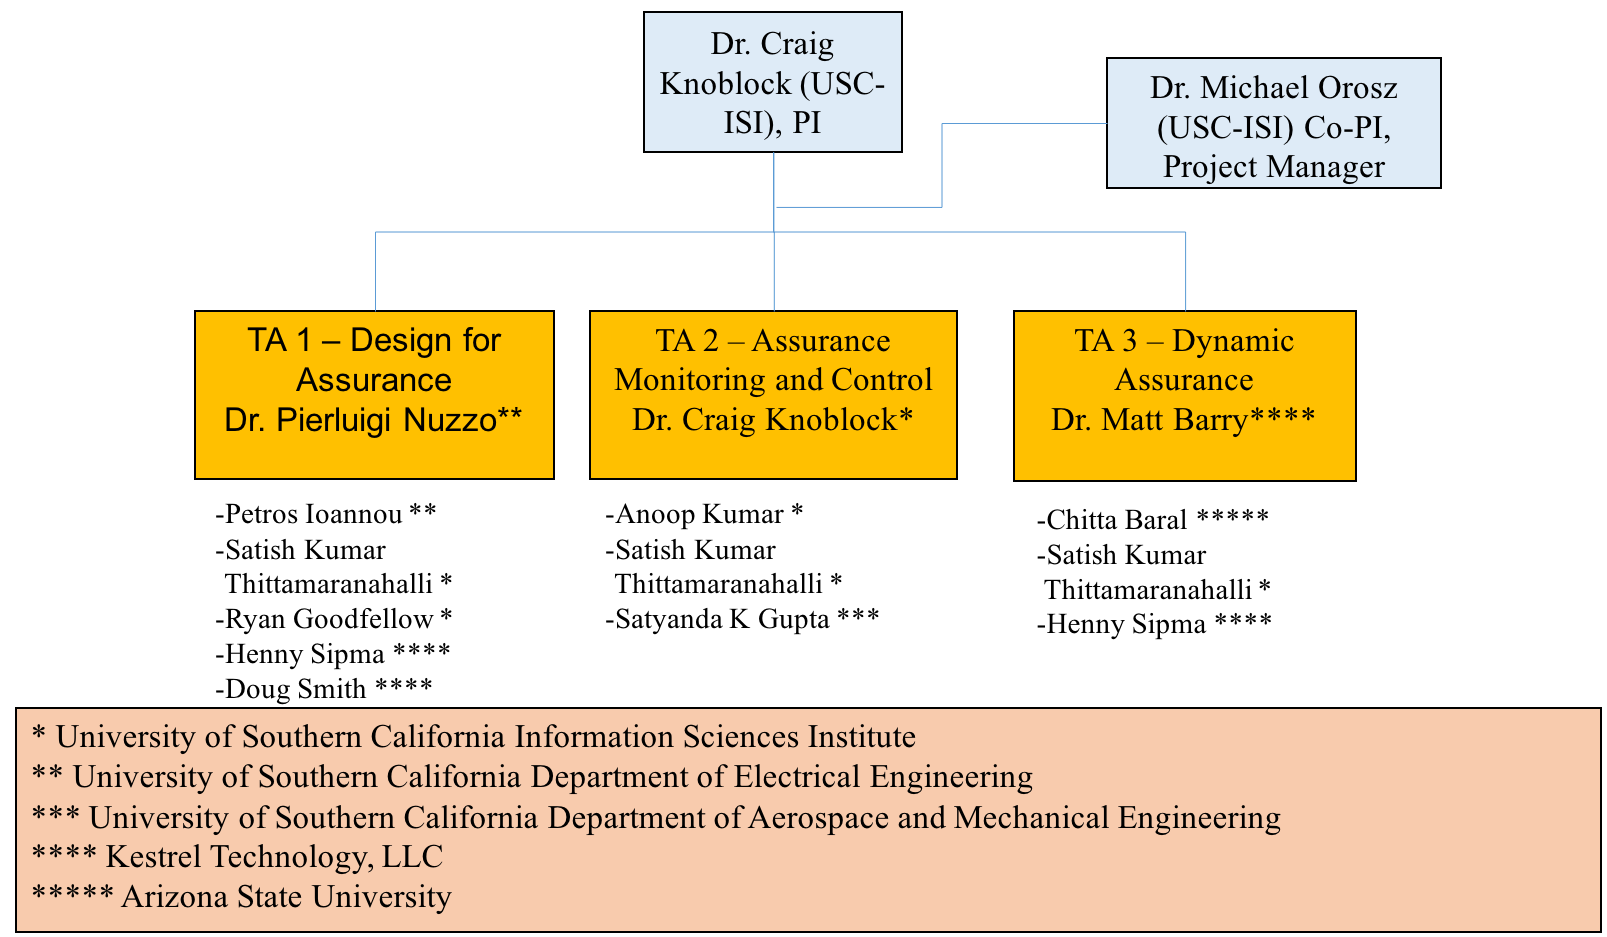
\includegraphics[width=6.0in]{./org-chart2.png}
\caption{\small Organization Chart}
\label{fig:org_chart}
\end{figure}

Coordination: To maximize collaboration and reduce risk to project failure from lack of communication and technical exchange, we plan to employ a wide variety of working styles and communication/coordination so that all can contribute.  At the core of our project will be regularly scheduled meetings bridging the diversely distributed team (Table~\ref{fig:Collaboration_Table}).  These meetings will address project status, identify challenges, implement risk mitigation strategies and participate in technology exchanges and system integration efforts (when appropriate)

\begin{table}[ht]
\caption{\small Project Meetings and Events}
  \centering
  {\footnotesize
\begin{tabular}{|m{3.15in}|m{3in}|} 
\hline
\textbf{Meeting} & \textbf{Frequency} 
\\\hline
Conference calls among investigators (discuss project status, address concerns and project risks) & Weekly
\\
\hline
Technical exchange and coordination meetings using Bluejeans or another videoconference technology & At least twice a month and more frequently as needed
  \\ 
\hline
Face-to-Face meetings (prior to P/I and demonstration meetings) & Every 3 to 6 months and more frequently (especially at the beginning of the project) as needed
 \\\cline{1-2}

\hline
\end{tabular}
}
\label{fig:Collaboration_Table}
\end{table}

\begin{table}[tbhp]
\caption{\small Key Project Team Member Responsibilities}
  \centering
  {\footnotesize
\begin{tabular}{| m{.75in} | m{3.9in}| m{1.5in}|} 
\hline
\textbf{Key Member} & \textbf{Responsibilities} & \textbf{Tasks} 
\\\hline
Dr.\ Craig Knoblock  & Principal Investigator responsible for project, leads TA 2 – Assurance Monitoring and Control.  Will lead the overall project and lead the TA2 team.  Served as the PI on many DARPA projects and has sucessfully led many large teams.    Effort on project:  25\% &
1.1.6, 1.2.2 1.2.3, 1.2.4, 1.3.4, 1.4.1, 
2.1.6, 2.2.2 2.2.3, 2.2.4, 2.3.4, 2.4.1, 
3.1.6, 3.2.2, 3.2.3, 3.2.4, 3.3.4, 3.4.1
\\
\hline
Dr.\ Michael Orosz & Co-Principal Investigator responsible managing the day-to-day operations of the project, assist technical teams as needed, coordinate with TA4 teams.    Has led many large complex multi-disciplined/multi-organizational projects in academic and industry environments.  Effort on project: 50\%
& 1.1.6, 2.1.6, 3.1.6, 1.4.1, 2.4.1, 3.4.1
  \\ 
\hline
Dr.\ Pierluigi Nuzzo 
& 
Co-Principal Investigator.  Leads the TA 1 - Design for Assurance team and conducts research on the formal methods for the design of the TA1 system.  Research experience on methodologies and tools for the design of cyber-physical systems; contracts, interfaces, and compositional methods for embedded system design; the application of automated formal methods and optimization theory to problems in embedded and cyber-physical systems.  Effort on project: 2 months/year (16.6\%)
& 
1.1.1, 2.1.1, 3.1.1 \\
\hline
Dr.\ Matthew Barry
& 
Key personnel.  Leads the TA 3 – Dynamic Assurance.   He will conduct the research on the dynamic assurance case language editors and parsers, the run-time system, and system integrations. Effort on project:  66\%
& 
1.3.2, 2.3.2, 3.3.2\\
\hline
Dr.\ Chitta Baral
& 
Key personnel responsible for learning assurance rules, supporting assurance rules with uncertainty and improving solver speed.  Expertise on ASP solvers, which will be used to reason about the assurance cases. Effort on project: 20\%
& 
1.3.1, 2.3.1, 3.3.1 \\
\hline
Dr.\ Doug Smith 
& 
Key personnel will support formal methods aspects of TA1, and lead the effort on abstract refinement. Expertise in field of automated correct-by-construction program generation.    Effort on project: 40\%
& 
1.1.5, 2.1.5, 3.1.5 \\
\hline
Dr.\ Henny Sipma
& 
Key personnel who will support the program verification tasks under TA1.  Will lead the effort on program verification.   Effort on project:  45\%
& 
1.1.5, 2.1.5, 3.1.5, 1.3.2, 2.3.2, 3.3.2 \\
\hline
Dr.\ Petros Ioannou
& 
Key personnel responsible providing and extending the assurance test bed, which will be available at the start of the project for autonomous vehicles.   Effort on project: 1 month/year (8.3\%)
& 
1.1.2, 2.1.2 (optional), 3.1.2 (optional)
\\
\hline
Dr.\ Satyandra Kumar Gupta
& 
Key Personnel providing autonomous command and control expertise to the TA-2 team.   Will lead the research on safety aware learning on TA2.   Past research on physics-aware decision making to facilitate automation.  Effort on project: 1 month/year (8.3\%)
& 
1.2.1, 2.2.1, 3.2.1 \\
\hline
Dr.\ Anoop Kumar 
& 
Key personnel providing support to the TA 2 project team.  Will lead the research on monitoring \& control and detecting distribution shifts.  Effort on project: 50\%
& 
1.2.1, 1.2.2, 1.2.3, 1.2.4, 2.2.1, 2.2.2, 2.2.3, 2.2.4, 3.2.1, 3.2.2, 3.2.3, 3.2.4\\
\hline
Dr.\ Satish Thittamaranahalli
& 
Key personnel developing scalable algorithms for TA1, TA2, and TA3 project teams.  Has extensive experience on scalable algorithm design, machine learning, and constraint reasoning.  Effort on project: 50\%
& 
1.2.1, 1.2.2, 1.2.3, 1.2.4, 2.2.1, 2.2.2, 2.2.3, 2.2.4, 3.2.1, 3.2.2, 3.2.3, 3.2.4, 1.1.4, 2.1.4, 3.1.4 \\
\hline
Dr.\ Ryan Goodfellow
& 
Key personnel providing support to the TA-1 project. Will lead the research on simulation-based testing.  Has extensive experience on simulation-based testing.  Effort on project:  30\%
& 
1.1.3, 2.1.3, 3.1.3 \\

\cline{1-2}

\hline
\end{tabular}
}
\label{fig:Table_Mgmt}
\end{table}



\newpage
\section{Personnel, Qualifications and Commitment}

{\bf Dr.\ Craig Knoblock}, the PI on this effort, is a Research Professor of both Computer Science and Spatial Sciences at the University of Southern California (USC) and Director of the Intelligent Systems Division at the USC Information Sciences Institute.   He received his Ph.D. from Carnegie Mellon University in computer science. 
%His research focuses on techniques for describing, acquiring, and exploiting the semantics of data.  
In previous projects he has worked on developing  scalable approaches to execution monitoring, accurate detection of sensor failures, and   automatic modeling and reconstruction of sensors.  He has published more than 300 journal articles, book chapters, and conference papers on these topics.  Dr. Knoblock is a Fellow of the Association for the Advancement of Artificial Intelligence (AAAI), a Distinguished Scientist of the Association of Computing Machinery (ACM), a Senior Member of IEEE, past President and Trustee of the International Joint Conference on Artificial Intelligence.
%and winner of the 2014 Robert S. Engelmore Award.  

{\bf Dr.\ Michael Orosz}, a Co-PI on this effort, is a Research Associate Professor of Civil and Environmental Engineering at the University of Southern California (USC) and Research Director of the Decision Systems Group at the USC Information Sciences Institute.  Dr. Orosz has over 30 years’ experience in commercial and government software development, basic and applied research, project management, academic research and has developed and deployed several commercially successful products.  His research interests are in machine learning and decision analytics as applied to intelligence analysis and autonomous command and control such as smart building controls.    Dr. Orosz has extensive experience in managing large complex multi-disciplined/multi-teamed research projects. %funded by DARPA, DHS, DoD, DoE, Industry, NASA, NRO, NSA and ONR.   
He received his Ph.D. in computer science from the University of California, Los Angeles.

{\bf Dr.\ Pierluigi Nuzzo}, a Co-PI on this project, is an Assistant Professor in the Department of Electrical Engineering at the University of Southern California. He received the Ph.D. in Electrical Engineering and Computer Sciences from the University of California at Berkeley. 
%in 2015, and the Laurea degree (MS) in electrical engineering (summa cum laude) from the University of Pisa, Italy, and the Sant'Anna School of Advanced Studies, Pisa, Italy.
%
%He has four years of research experience in analog and mixed signal circuit design as a researcher at IMEC, Leuven, Belgium, and over 10 years experience in design methodologies and tools for mixed-signal integrated circuits and cyber-physical systems, as a researcher at the University of Pisa, IMEC, UC Berkeley, and USC. 
His research interests
include: methodologies and tools for cyber-physical system and mixed-signal
system design; contracts, interfaces and compositional methods for embedded
system design; the application of formal methods and optimization theory to problems in embedded and cyber-physical systems and electronic design automation. 
%
Prof. Nuzzo received %First Place in the operational category and Best Overall
%Submission in the 2006 DAC/ISSCC Design Competition, 
a Marie Curie Fellowship
from the European Union in 2006, 
the University of California at Berkeley EECS
departmental fellowship in 2008, 
%the University of California at Berkeley Outstanding Graduate Student Instructor Award in 2013, 
the IBM Ph.D.
Fellowship in 2012 and 2014, 
%the Best Paper Award from the International Conference on Cyber-Physical Systems (ICCPS) in 2016, 
and the David J.~Sakrison Memorial Prize in 2016 for his doctoral research. 
%He is an author of 1 patent and over 60 publications.

{\bf Dr.\ Satyandra K. Gupta} is Smith International Professor in the Department of Aerospace and Mechanical Engineering at the University of Southern California. %Prior to joining the University of Southern California, he was a Professor in the Department of Mechanical Engineering and the Institute for Systems Research at the University of Maryland. He was the founding director of the Maryland Robotics Center and the Advanced Manufacturing Laboratory at the University of Maryland. 
He served as a program director for the National Robotics Initiative at the National Science Foundation from September 2012 to September 2014.  Dr. Gupta's interest is in the area of physics-aware decision making to facilitate automation. He has published more than 300 technical articles. He is a fellow of the American Society of Mechanical Engineers (ASME) and editor of ASME Journal of Computing and Information Science in Engineering. Dr. Gupta has received the Young Investigator Award from the Office of Naval Research in 2000, CAREER Award from the National Science Foundation in 2001, Presidential Early Career Award for Scientists and Engineers (PECASE) in 2001, Invention of the Year Award at the University of Maryland in 2007, Kos Ishii-Toshiba Award from ASME in 2011, and Excellence in Research Award from ASME in 2013.%, and Distinguished Alumnus Award from Indian Institute of Technology, Roorkee in 2014. %He has also received seven best paper awards at conferences.

{\bf Ryan Goodfellow} is a computer scientist at ISI working in combined cyber physical simulation and emulation platform development. His formal background is in simulation algorithms and modeling techniques using differential-algebraic equations (DAE). He has applied this knowledge in the CPS space by integrating DAE modeling languages and simulation engines with network testbeds to create comprehensive scientific experimentation platforms for cyber-physical systems. These experimentation platforms have been used in the power grid research space. %Ryan is a lead developer on the Deter network testbed, with a strong background in networked and distributed systems engineering. %He is also a combat veteran, serving as a non-commissioned officer and SIGINT team lead for a multi-functional intelligence team in Afghanistan.

{\bf Dr.\ Petros Ioannou} is a Professor in the Department of Electrical Engineering, Director of the Center for Advanced Transportation Technologies and Associate Director for Research for the DOT supported University Transportation Center at USC. He received his MS and PhD from the University of Illinois at Urbana Champaign in Mechanical and Electrical Engineering, respectively. His research interests are in robust adaptive control, vehicle dynamics and control, human factors and safety, automated vehicles, nonlinear systems and Intelligent transportation Systems.  He received the 2016 IEEE Transportation Technologies field award and the 2016 IEEE Control system society Transition to Practice Award. He is a Fellow of IEEE, IFAC and IET and author/coauthor of 8 books and over 400 papers.

{\bf Dr.\ Matthew Barry} will serve as lead for the TA3 tasks. %He will implement the dynamic assurance case language editors and parsers, the run-time system, and system integrations.  He will implement the assurance case arguments and the API for updating argument structure and content.  
Dr. Barry currently is CEO at Kestrel Technology LLC, and previously spent 20 years in NASA space mission operations at the Jet Propulsion Lab and Johnson Space Center.  At NASA Headquarters he led the introduction of dependability case requirements and plans for flight computing systems in upcoming manned space exploration missions, as well as the development of Agency-level software-related safety-critical control system requirements.  He recently served as a Principal Investigator on DHS/Cyber S\&T STAMP (Static Tool Analysis Modernization Program), DARPA CSFV (Crowd Sourced Formal Verification), three NASA Aeronautics R\&D projects, and the AFRL-sponsored Static Analysis of Numerical Algorithms project.  Dr. Barry earned BSME, MS, and PhD degrees in mechanical engineering, and an MBA degree, from Rice University.  

{\bf Dr.\ Henny Sipma} will support the program verification tasks under TA1.  %She is the key person behind the company's {\em KT Advance\/} and {\em KT Transferal\/} static analysis products, and the designer and programmer of the company's core {\em CodeHawk\/} abstract interpretation engine. 
Dr. Sipma currently is the CTO at Kestrel Technology LLC.  She has spent the past 10 years with Kestrel Technology as a static analysis expert; previously developed and taught static analysis techniques as senior research associate at Stanford University for eight years; and developed industrial process controls as an senior systems analyst at Shell.  She has been Principal Investigator or company lead on several recent R\&D projects for Federal agencies, including two projects under the IARPA STONESOUP (Securely Taking On New Executable Software of Uncertain Provenance) program; the DHS Cyber S\&T Gold Standard project; and the DARPA-sponsored STAC (Space-Time Analysis for Cybersecurity) and MUSE (Mining and Understanding Software Enclaves) programs.  Dr. Sipma earned 
%a BS degree in chemistry and an MS degree in chemical engineering at the University of Groningen in The Netherlands, and 
MS and PhD degrees in computer science from Stanford University.  

{\bf Dr.\ Douglas R.\ Smith} will support formal methods aspects of TA1, including the enforcement of safety properties and the generation of monitors.  He is President of Kestrel Technology LLC and Principal Scientist at Kestrel Institute.  He is a Fellow of the American Association of Artificial Intelligence (AAAI) and an ASE Fellow (Automated Software Engineering).  From 1986 to 2000, he taught an advanced graduate course on correct-by-construction software development at Stanford.  
%Dr. Smith has led the development of a series of software synthesis systems, including KIDS (Kestrel Interactive Development System), Specware, Designware, and Planware. 
%Applications domains have included a variety of complex high-performance planners and schedulers for the US Air Force.  He leads current projects on the generation of air mission plans and cyberoperations.  
Other recent projects focused on automated policy enforcement \cite{SmithD0703,SmithD08}, synthesis of secure network protocol codes, and the synthesis of high-performance constraint-solvers\cite{SmithD08c,SmithD13}.  Dr. Smith has over 30 years experience in the field of automated correct-by-construction program generation and has published over 100 papers. He has one patent.  He received the Ph.D. in Computer Science from Duke University% in 1979.  

{\bf Dr. Chitta Baral} is a Professor in the Department of Computer Science and Engineering at Arizona State University. He will support the TA3 efforts on Learning assurance rules, supporting assurance rules with uncertainty and improving solver speed. Dr. Baral has expertise in various aspects of autonomy and Artificial Intelligence. 
He wrote the first book on answer set programming (published by Cambridge University Press) the formal language behind our assurance rules. Some of his other works relevant to this proposal are: goal specification for autonomous systems, automatic construction of control rules for autonomous systems that satisfy given goals, combining machine learning with reasoning in various contexts, including image understanding. %He is the President of KR Inc. He is an associate editor of AIJ and has been an associate editor of JAIR.

{\bf Dr.\ Satish Kumar Thittamaranahalli (T. K. Satish Kumar)} leads the Collaboratory for Algorithmic Techniques and Artificial Intelligence (CATAI) at USC's Information Sciences Institute. He has published over 60 papers on numerous topics in Artificial Intelligence spanning such diverse areas as Constraint Reasoning, Planning and Scheduling, Probabilistic Reasoning, Robotics, Combinatorial Optimization, Approximation and Randomization, Heuristic Search, Model-Based Reasoning, Knowledge Representation and Spatio-Temporal Reasoning. %He %has served on the Program Committees of many international conferences in Artificial Intelligence
He and is a winner of the 2016 Best Robotics Paper Award and the 2005 Best Student Paper Award from the International Conference on Automated Planning and Scheduling. 
Dr. Kumar received his PhD in Computer Science from Stanford University. %In the past, he has also been a Visiting Student at the NASA Ames Research Center, a Postdoctoral Research Scholar at the University of California, Berkeley, a Research Scientist at the Institute for Human and Machine Cognition, a Visiting Assistant Professor at the University of West Florida, and a Senior Research and Development Scientist at Mission Critical Technologies.

\textbf{Dr.\ Anoop Kumar} is a senior computer scientist at USC ISI and has broad expertise in machine learning, statistical modeling, and software engineering.  Dr.\ Kumar is the technical lead on the DARPA RSPACE program and has played a vital role in developing a system that fuses air operations data from multiple sources, maintains world state, and issues warnings. Previously, he led the research and development of the BBN’s election forecasting system for the IARPA OSI program. %Dr.\ Kumar played a significant role in the DARPA DEFT program by developing a model to support integration of output from multiple NLP algorithms. He has contributed at the development to management levels on government research contracts and commercial projects. 
Dr.\ Kumar helped design and develop BBN's commercially available, hosted speech and medical transcription services offering. 

\begin{table}[!tbh]
\begin{footnotesize}
\vspace{-0.1in}

\begin{tabular}{lll}
\begin{tabular}[t]{|l|@{}c@{}|@{}c@{}|@{}c@{}|@{}c@{}|} \hline
Project & Status & \multicolumn{3}{ c| }{Hours} \\ \cline{3-5}
& & P1 & P2 & P3 \\ \hline



\multicolumn{5}{ |c| }{ \textbf{Craig Knoblock} } \\ \cline{1-5}
Safeguard & Pro & 770 & 641 & 641 \\ \cline{1-5}
ELICIT & Cur & 308 & 256 & 120 \\ \cline{1-5}
WTNIC & Cur & 11 & 0 & 0 \\ \cline{1-5}
EFFECT & Cur & 641 & 107 & 0 \\ \cline{1-5}
LinkedMaps & Cur & 203 & 25 & 0 \\ \cline{1-5}
PRINCESS & Cur & 608 & 96 & 0 \\ \cline{1-5}
SCHARP & Cur & 481 & 54 & 0 \\ \cline{1-5}
MINT & Pen & 650 & 534 & 285 \\ \cline{1-5}

\multicolumn{5}{ |c| }{ \textbf{Michael Orosz} } \\ \cline{1-5}
Safeguard & Pro & 1560 & 1300 & 1300  \\ \cline{1-5}
SMC/SY & Cur & 1803 & 0 & 0  \\ \cline{1-5}

\multicolumn{5}{ |c| }{ \textbf{Matthew Barry} } \\ \cline{1-5}
Safeguard & Pro & 2078 & 1690 & 1554 \\ \cline{1-5}
Starlite & Cur & 1840 & 1692 & 0 \\ \cline{1-5}



\multicolumn{5}{ |c| }{ \textbf{Anoop Kumar} } \\ \cline{1-5}
Safeguard & Pro & 1560 & 1300 & 1300 \\ \cline{1-5}

\end{tabular}
&
\begin{tabular}[t]{|l|@{}c@{}|@{}c@{}|@{}c@{}|@{}c@{}|} \hline
Project & Status & \multicolumn{3}{ c| }{Hours} \\ \cline{3-5}
& & P1 & P2 & P3 \\ \hline

\multicolumn{5}{ |c| }{ \textbf{Pierluigi Nuzzo} } \\ \cline{1-5}
Safeguard & Pro & 520 & 433 & 433  \\ \cline{1-5}
Mirage & Cur & 433 & 0 & 0  \\ \cline{1-5}

\multicolumn{5}{ |c| }{ \textbf{Satyandra Gupta} } \\ \cline{1-5}
Safeguard & Pro & 260 & 217 & 217 \\ \cline{1-5}
Human   & Cur & 22 & 0 & 0 \\ \cline{1-5}
Vehicles & Cur & 36 & 0 & 0 \\ \cline{1-5}
Robot & Cur & 116 & 0 & 0 \\ \cline{1-5}
Assembly & Cur & 33 & 0 & 0 \\ \cline{1-5}
Solar & Cur & 4 & 0 & 0 \\ \cline{1-5}

\multicolumn{5}{ |c| }{ \textbf{Petros Ioannou} } \\ \cline{1-5}
Safeguard & Pro & 260 & 217 & 217 \\ \cline{1-5}
CPS & Cur & 130 & 0 & 0 \\ \cline{1-5}

\multicolumn{5}{ |c| }{ \textbf{Ryan Goodfellow} } \\ \cline{1-5}
Safeguard & Pro & 936 & 780 & 780 \\ \cline{1-5}
STEAM & Cur & 416 & 0 & 0 \\ \cline{1-5}


\end{tabular}
&
\begin{tabular}[t]{|l|@{}c@{}|@{}c@{}|@{}c@{}|@{}c@{}|} \hline
Project & Status & \multicolumn{3}{ c| }{Hours} \\ \cline{3-5}
& & P1 & P2 & P3 \\ \hline

\multicolumn{5}{ |c| }{ \textbf{Chitta Baral} } \\ \cline{1-5}
Safeguard & Pro & 659 & 485 & 485 \\ \cline{1-5}
PostdocBP & Cur & 176 & 0 & 0 \\ \cline{1-5}
Languages & Pen & 528 & 264 & 264 \\ \cline{1-5}
CAREER & Pen & 88 & 44 & 44 \\ \cline{1-5}
CHS & Pen & 510 & 255 & 0 \\ \cline{1-5}

\multicolumn{5}{ |c| }{ \textbf{Doug Smith} } \\ \cline{1-5}
Safeguard & Pro & 1222 & 984 & 840 \\ \cline{1-5}
RSPACE & Cur & 342 & 0 & 0 \\ 
\cline{1-5}
PLANX & Cur & 154 & 0 & 0 \\ 
\cline{1-5}
HACCS & Pen & 923 & 769 & 769 \\ 
\cline{1-5}

\multicolumn{5}{ |c| }{ \textbf{Henny Sipma} } \\ \cline{1-5}
Safeguard & Pro & 1372 & 962 & 840 \\ \cline{1-5}
STAC & Cur & 797 & 0 & 0 \\ \cline{1-5}

\multicolumn{5}{ |c| }{ \textbf{Satish Thittamaranahalli} } \\ \cline{1-5}
Safeguard & Pro & 1560 & 1300 & 1300 \\ \cline{1-5}
MapF & Cur & 103 & 103 & 0 \\ \cline{1-5}

\end{tabular}
\end{tabular}

\end{footnotesize}
\caption{Individual commitments of key personnel}
\label{tab:Commitments}
\vspace{-0.2in}
\end{table}

\clearpage
\newpage
\section{Capabilities}


%\subsection{University of Southern California}
USC has strengths in number of areas that are closely related to the proposed work:
\begin{itemize}[itemsep=0pt,leftmargin=*]
\item Dr.\ Nuzzo 
%has over 10-year research experience in embedded system design, from mixed-signal chip design (analog-to-digital converters, frequency synthesizers, software-defined radio), to methodologies and tools for mixed-signal integrated circuits and Cyber-Physical Systems (CPSs), and the application of formal methods and optimization theory to problems in embedded and cyber-physical systems and electronic design automation.  
%His doctoral work 
has done extensive research on contracts and compositional methods for heterogeneous system design and design space exploration, with application to aircraft electric power systems and environmental control systems. His work has helped transition rigorous system design foundations, innovative design methodologies, and new systems engineering paradigms to industry (IBM, United Technologies). 
\item Dr.\ Satyandra K. Gupta has worked on autonomous surface vehicles, autonomous ground vehicles for operation on rugged terrains, and autonomous flapping wing aerial vehicles.   His group has developed a hierarchal decision making approach for realizing autonomous systems. 
%This approach combines task planning and assignment, deliberative trajectory planning, reactive collision avoidance behaviors, and trajectory tracking control layers. 
His group has also developed new methods for learning reactive behaviors in adversarial environments and COLREGS compliant trajectory planning. \item Dr.\ Knoblock has developed methods that learn the relationships between sensors to both identify failures and changes in sensor and reconstruct those sensors, providing estimates of the accuracy of the reconstructed sensors.  
\item Ryan Goodfellow has extensive experience in simulation based testing through high-fidelity CPS testbed environment development and operation, using the Deter network testbed as the core which has supported several large scale government projects from a variety of agencies and thousands of users. %we have developed sophisticated CPS experiments under programs such as NFS RIPS, NIST SmartCities and the DHS Cybersecurity showcase.
\item Dr.\ Ioannou %helped  design and implement adaptive cruise control systems in collaboration with Ford Motor Company, which was commercialized four years before any other company. He 
worked on several DOT funded projects on automated vehicles and intelligent highway systems where he demonstrated his vehicle control designs for safety and performance on actual automated vehicles in test trucks and I-15 highway.
\item Drs.\ Knoblock, Kumar, and Thittamaranahalli have developed highly scalable approaches for monitoring message traffic to identify potential problems and issue warnings and alerts. 
\item Dr. Thittamaranahalli has developed state-of-the-art methods for efficiently solving large-scale search and optimization problems. %These techniques will be applicable in TA2 for safety-aware learning and planning, in TA2 for assurance monitoring and control, and in TA3 for dynamic assessment of assurance cases.

\end{itemize}
%\subsection{Kestrel Technology LLC}

Kestrel Technology's strength is in program analysis, specifically static analysis of both source and binary targets.  The company performs applied R\&D and product development for a variety of static analysis applications  pivoting primarily on the abstract interpretation technique.  The company recently initiated development of program analysis applications using logical equivalence techniques. As a provider of verification evidence in the form of mathematical proofs, the company also has expertise in the design and development of assurance case arguments for high-integrity systems using such evidence. %The company is engaged in a partnership with Wind River Systems to develop program analysis tools for its embedded system developers.  Many of Wind River's customers must develop their products under safety and certification standards, including those using safety cases.  

   

%\subsection{Arizona State University}
Chitta Baral at Arizona State University has developed various software to learn assurance rules and various ASP solvers, which he has made available as open-source.

Most of the software carried forward for implementation or derivation is open source.  The single exception is Kestrel Technology's {\it KT Advance\/} static analysis tool (TA1), in particular the abstract interpretation engine therein, which is company proprietary and is US EAR export-controlled.   
%Owing to mixed funding for the development of that technology 
We will continue to provide the Federal government a restricted use license for that particular item.

There are no specialized facilities, data, or GFE required for this effort. 

\include{sow}
\include{milestones}

% \section{Level of Effort by Task \textcolor{red}{[Mike/Lisa - 1 pages]}}

% \textcolor{blue}{
% \begin{itemize}
% \item Will be a separate spreadsheet
% \item
% \end{itemize}
% }

\include{appendix_a}

%\section{Appendix B \textcolor{red}{[No Page Count]}}

\section{References}
\bibliographystyle{acm} 
\bibliography{TA3/ta3,TA2/ta2,TA1/ta1}
\end{document}
%%\documentclass[a4paper]{article}
%\documentclass[12pt]{article}
\documentclass[12pt]{dod-blank}

%% Language and font encodings
\usepackage[english]{babel}
\usepackage[utf8x]{inputenc}
\usepackage[T1]{fontenc}

%% Sets page size and margins
%%\usepackage[a4paper,top=3cm,bottom=2cm,left=3cm,right=3cm,marginparwidth=1.75cm]{geometry}
%\usepackage[top=1in, bottom=1in, left=1in, right=1in]{geometry}



%% Useful packages
\usepackage{amsmath}
\usepackage{graphicx}
  \graphicspath{{.}{./image/}}
  \DeclareGraphicsExtensions{.png,.jpg} 
\usepackage[colorinlistoftodos]{todonotes}
\usepackage[colorlinks=true, allcolors=blue]{hyperref}
\usepackage{tabularx}
\usepackage{multirow}
\usepackage{tabulary}
\usepackage{float}
\usepackage{wrapfig}
\usepackage[export]{adjustbox}
\usepackage{comment}
\usepackage{tabularx}
\usepackage{multirow}
\usepackage{tabulary}
\usepackage{enumitem}

\usepackage{listings}
\usepackage{color}
\usepackage{array}
\usepackage{subcaption}
\usepackage{xcolor}




\renewcommand{\textfraction}{0}
\renewcommand{\topfraction}{1.0}
\renewcommand{\bottomfraction}{1.0}

\usepackage{longtable}
%% macros
\newif\iffinal
\finaltrue
\iffinal
  
    \newcommand\baareq[1]{}
    \newcommand\baades[1]{}
 
 
\else
    \definecolor{darkgreen}{rgb}{0,0.4,0}
    \definecolor{darkcyan}{rgb}{0,0.4,0.4}
    \definecolor{darkblue}{rgb}{0,0,0.5}
    
    \newcommand\baareq[1]{{\color{darkcyan}[\textbf{Requirement:} #1]}}
    \newcommand\baades[1]{{\color{darkcyan}[\textbf{Description:} #1]}}
 
\fi




\def\naive{na\"{\i}ve}



\lstset{ 
  backgroundcolor=\color{white},   % choose the background color; you must add \usepackage{color} or \usepackage{xcolor}
  basicstyle=\footnotesize\ttfamily,            % the size of the fonts that are used for the code
  breakatwhitespace=false,         % sets if automatic breaks should only happen at whitespace
  breaklines=true,                 % sets automatic line breaking
  captionpos=b,                    % sets the caption-position to bottom
  commentstyle=\color{mygreen},    % comment style
  % deletekeywords={...},            % if you want to delete keywords from the given language
  escapeinside={\%*}{*)},          % if you want to add LaTeX within your code
  extendedchars=true,              % lets you use non-ASCII characters; for 8-bits encodings only, does not work with UTF-8
  frame=single,	                   % adds a frame around the code
  keepspaces=false,                 % keeps spaces in text, useful for keeping indentation of code (possibly needs columns=flexible)
  keywordstyle=\color{blue}\bfseries\underbar,       % keyword style
  language=Prolog,                 % the language of the code
  % morekeywords={if,and},        % if you want to add more keywords to the set
  numbers=none,                    % where to put the line-numbers; possible values are (none, left, right)
  numbersep=5pt,                   % how far the line-numbers are from the code
  numberstyle=\tiny\color{mygray}, % the style that is used for the line-numbers
  rulecolor=\color{black},         % if not set, the frame-color may be changed on line-breaks within not-black text
  showspaces=false,                % show spaces everywhere adding particular underscores; it overrides 'showstringspaces'
  showstringspaces=false,          % underline spaces within strings only
  showtabs=false,                  % show tabs within strings adding particular underscores
  stepnumber=2,                    % the step between two line-numbers. If it's 1, each line will be numbered
  stringstyle=\color{mymauve},     % string literal style
  tabsize=2,	                   % sets default tabsize to 2 spaces
  title=\lstname                   % show the filename of files included with \lstinputlisting; also try caption instead of title
}

% apply trick for additional keywords for our AC DSL
\lstset{
	emph={for, if, and, or},
    emphstyle={\color{blue}\bfseries\underbar}
}




\title{DARPA Assured Autonomy}
\author{Technical Volume- \textcolor{red}{Thirty-Eight (38) pages max}}

\begin{document}
\pagenumbering{roman}
\include{cover}

\newpage
\section{Table of Contents}
\tableofcontents

\newpage
\pagenumbering{arabic}
\section{Executive Summary}
As we rapidly move into a world where machine learning plays a central role in realizing autonomous systems, it is becoming increasingly important to develop techniques that assure that these systems will operate safely and perform as expected. Current approaches are limited to providing assurance for systems with limited or no  learning capabilities. In this context, DARPA's Assured Autonomy BAA seeks to \emph{develop rigorous design and analysis technologies for continual assurance of learning-enabled autonomous systems}. USC in collaboration with Kestrel Technology and ASU is pleased to submit a comprehensive TA1, TA2, and TA3 proposal entitled \emph{``Assured Autonomy for Learning Enabled Vehicles (Safeguard).''} We plan to provide an end-to-end solution to support autonomous systems with learning-enabled components, ranging from design technologies for assurance, to assurance monitoring and control techniques, to representation and online evaluation of assurance cases. We have assembled a strong team of experts that cover the range of technologies that are required to create such an end-to-end system. If successful, the project will provide the technologies for building the next-generation of learning-enabled autonomous systems.  The entire project will take four years and cost \textcolor{red}{\$??}, with an initial version completed at the end of Phase I and successive versions with additional capabilities and improved scalability at the end of Phase II and Phase III.  

In the remainder of this section, we first introduce an  unmanned surface vehicle scenario that will be used throughout the proposal to describe the approach.  Next, we describe our approach to design, monitoring, and dynamic assurance. Finally, we introduce the team involved in the project. 

\textbf{Motivating Scenario.} Consider an autonomous unmanned surface vehicle (USV) guarding a valuable asset in the ocean when an unknown vehicle  approaches the security perimeter, under challenging weather conditions. In this scenario, the USV is required to approach the intruding vehicle, issue a warning signal, and escort it to a safe distance from the controlled area. However, as the USV has no a priori knowledge of its external environment behaviors (e.g., water depth, waves, wind, current, visibility), pre-computing a feasible trajectory, let alone optimal, becomes a non-trivial problem. For trajectory planning, the USV must continuously perform the following tasks:
\begin{itemize}[itemsep=0pt,leftmargin=*]
 \item Sense the current state of the surrounding environment (e.g., water depth, waves, wind, current, visibility) and estimate its own maneuverability constraints (e.g., braking distance, available acceleration, maximum velocity, turning radius, turning rate, safety distance) based on the state of the environment;      
\item Sense the static obstacles in the sensor range and generate a traversability map;
\item Sense the moving obstacles and classify them;   
\item Predict future trajectories of moving obstacles; 
\item Determine if any of the COLREGS \cite{commandant1999international} rules will be in effect with respect to one or more of the nearby vessels and identify the vessels with the right of way.    
\end{itemize}
The above information will be used by the trajectory planner to compute an initial trajectory, which will be continuously refined as the USV gathers additional information.
% It is not possible for the USV to be tested in every possible environment. 
The USV will use learning enabled components to take  decisions as it encounters new situations, such as  
\begin{itemize}[itemsep=0pt,leftmargin=*]
\item Classifiers to identify moving obstacles based on physical appearance and motion signatures,
\item Algorithms to estimate the sensor capabilities in adverse weather conditions,   
\item Algorithms to accurately estimate uncertainty in the environment, 
\item Classifiers to generate traversability maps,
\item Prediction of external vessel behaviors based on motion histories, 
\item Reinforcement learning  to ensure COLREGS compliance of maneuvers,  
\item Algorithms to learning pursuit behaviors.  
\end{itemize}
Learning enabled components will interact with each other in complex ways, where a misclassification error in one component may eventually compromise the entire mission.   
% We will need to make sure that each learning enabled components has a run-time monitor that will ensure that the assumptions made by the learning-enabled component remain valid and prevent erroneous learning. 
% For example, if the vehicle is exhibiting significant error in trajectory tracking, then simply downgrading the trajectory tracking error value may not be a good option.  The failure of prediction of trajectory tracking error might be due to the presence of a significant wake caused by a nearby vessel. The presence of the nearby vessel can be used to explain the degradation in trajectory tracking performance. As the vessel moves away, we can expect the trajectory tracking performance to return to the predicted level.  
While exhaustive validation of learning-enabled cyber-physical systems (LE-CPSs) is a prohibitive task~\cite{Kalra16},
their complexity, heterogeneity, and highly dynamic nature
make it challenging to even leverage existing model-based development techniques to effectively assess system correctness 
% dependability, 
at design time or enforce it at runtime.

\textbf{Design for Assurance.} Safeguard uses a platform-based design approach~\cite{Nuzzo15b} to organize the design process for a LE-CPS and to build assurance cases. Composite models are developed at several levels of abstraction,
from top-level system requirements and safety constraints down to the
implementation level.  Intermediate levels add detail to the levels
above.  The different levels are connected by refinement mappings that
allow properties established at one level to be preserved at the next
level (see Figures~\ref{fig:methodology} and~\ref{fig:assurance}).

Contracts are used to formally specify components and composite models
in terms of (1) Assumptions -- the assumed behaviors of the
environment and the behaviors of other components, and (2) Guarantees
-- the behavior properties that a model guarantees if it operates in a
context that satisfies its assumptions.  A calculus of contracts
allows horizontal composition of contracts to generate contracts for
composite models.  Vertical contracts are used to specify the mapping
or refinement relation between models at different levels of
abstraction.  The system design process starts with a high-level
contract that expresses overall system assumptions and requirements.
Subsequent levels express models with increasing detail until the
lowest level expresses the system in terms of hardware components and
their software controllers.

The assurance case for a CPS arises from the horizontal and vertical
structure of the design in several ways.  The components used within a
particular level are either (1) synthesized using
correct-by-construction design tools together with proofs, (2) derived
statically or dynamically using safety-aware machine-learning
techniques, (3) written manually and verified by analysis tools, or
(4) written manually and validated by extensive testing.  The
assurance case for the whole reflects its compositional structure.  We
anticipate that well-specified contracts together with the calculus of
contracts will eliminate well-known problems with unexpected emergent
behaviors in CPS systems.

The assurance case for the lowest-layer design arises from both the
intra-level assurance and from properties and their proofs that are
preserved under the refinement mapping from the top-level
requirements.  The refinement mappings between model layers will be
constructed using a variety of techniques.  A contract at an abstract
level can be mapped to a component or refined contract by (1)
retrieval of pre-verified components from a platform library, (2)
synthesis using correct-by-construction design and optimization tools,
or (3) manual coding to satisfy a contract.  The mapping of a
composite model will be composed from the mappings of its constituent
components or contracts.  When a composite model cannot be mapped
compositionally to the next level, it will be generated using
correct-by-construction design and optimization tools.

\textbf{Assurance Monitoring and Control.}
We provide an integrated framework for safety-aware learning, assurance monitoring and control, detecting distribution shifts. Three major components offer an efficient TA2 architecture as well as interfaces with TA1 and TA3, that is, (a) safety-aware learning and planning, (b) assurance monitors for guarding architectural and safety constraints; and (c) distribution shift detection.

We will develop a new learning-enabled online decision-making framework that allows opportunistically composing a sequence of actions (maneuvers) to reduce uncertainty in the system capability model without suspending the progress toward the mission goals or compromising safety. Each candidate action is evaluated based on three criteria: (1) the risk of violating a safety constraint using the current uncertainties in the parameter estimates; (2) its relevance to the mission goals; (3)  its expected information gain, i.e., reduction in uncertainty, with respect to the parameter estimates. These evaluations are combined to produce a cumulative mission utility value for each action that drives our learning-enabled decision-making framework. The problem of generating and evaluating sequences of actions can be posed in several way. For example, it can be solved using a branch-and-bound search method like Anytime A*, or formulated with the finite-horizon Markov Decision Process (MDP) framework. We will develop new scalable search strategies to solve this problem efficiently, by potentially evaluating a recent method developed at USC, called FastMap, that can significantly improve the execution time. 

We will develop monitors for architectural and safety constraints. 
% While these constraints can be checked over and over again as sensor information flow in, this naive strategy accounts for a lot of computational overhead. 
To achieve scalability and decrease the overhead, we propose the application of a technique that we currently use in DARPA's RSPACE program, which leverages a physical model of the vehicles dynamics and its interactions with the environment to efficiently determine the readout frequency. We propose two  extensions of this basic idea. First, we will use the theory of Variable Elimination to prioritize which variables to monitor, e.g., controllable, versus uncontrollable, adversarially controlled, or unobservable variables. Second, we invoke the dynamic assessment of assurance cases only when needed. This  decreases the number of times dynamic assessment of assurance cases is initiated as well as the communication bandwidth between the TA2 and TA3 components.

Finally, we will identify a distribution shift by combining statistical and machine learning techniques to differentiate between environmental and sensor changes. We will exploit a categorization of the shifts based on their cause and duration as well as extend our earlier work on detecting and mitigating sensor failures for all types of monitored variables.  

\textbf{Dynamic Assurance:} The Safeguard {\em design for assurance\/} activity takes a systems-theoretic stance toward safety.  Consequently, it presumes that safety is an emergent property of the system, and that hazards can present themselves through unintended interactions and performance violations in addition to causal events such as component failures.  Our design approach includes consideration of intent as well as hazard analysis and mitigation.  The artifacts from these activities populate contracts and assumptions for the dynamic assurance case.  
We thus build safety into the product by working at a systems-level viewpoint, using lexicon and design patterns familiar to both hardware and software engineers; safety is an emergent property of the system, not an afterthought.  
As system behavior evolves during runtime owing to learning, threats, degradation, or some other factor, the dynamic assurance case identifies whether the safety constraints continue to be satisfied.  If not, it provides notifications or issues recovery instructions directly from a lookup table.

Our implementation of the dynamic assurance case employs a declarative knowledge base inference engine and a domain-specific language tailored to our approach.  We have used them successfully for assurance case tool sets and arguments, and will extend them to reason about uncertainty and learning.  Our approach to achieve scalability is to specialize solvers toward modularity and to take advantage of domain knowledge.  Specifically, we will develop answer set programming techniques for context-dependent learning for reasoning about the learning-enabled components as well as learning assurance rules.  We will develop new formalisms for uncertainty to include causality, using weights for computing probabilities, and probabilistic non-monotonicity.  To achieve scaling objectives we will implement specializations using modularity, weighted CSPs, and message passing. 

% The system safety constraints revealed from that design become the key elements of our dynamic assurance case.  Our verification tools ensure the constraints are relevant, identifiable, and their implementation and effect observable.  

\textbf{Team.} We have assembled a team that is exceptionally well-qualified to build the proposed Safeguard system.  The team will be led by Dr.\ Craig Knoblock, the Principal Investigator for the effort, who currently leads the Intelligent Systems Division at the Information Sciences Institute.  He has led many large DARPA and IARPA projects over the years and has a strong track record in conducting leading edge research and then transitioning the technology to commercial use.  He will be supported by Dr.\ Michael Orosz as the Project Manager, who also has  experience in managing large research projects and on autonomous systems.  The TA1 team will be led by Dr.\ Pierluigi Nuzzo, who is an expert in embedded system design methodologies and the  application of formal methods to cyber-physical systems.  The TA1 team also includes Dr.\ Doug Smith, who has spent many years working on scalable correct-by-construction techniques and Dr.\ Henny Sipma, who has significant experience in applying program verification methods to real-world problems.  The TA1 team also includes Ryan Goodfellow, who has done a large amount of work on simulation-based testing.  The TA2 team will be led by Dr.\ Knoblock who has worked on topics related to both monitoring and detecting distribution changes.  He will be supported by Dr.\ Satyandra Gupta, who is an expert on autonomous surface vehicles as well as on safety-aware learning. He will also be supported by Drs.\ Anoop Kumar and Satish Thittamaranahalli, who have also previously worked on efficient methods for execution monitoring.  The TA3 team will be lead by Dr.\ Matthew Barry, who has experience in creating the technologies for assurance cases.  He will be supported by Dr.\ Chitta Baral, who is an expert on ASP solvers and by Dr.\ Thittamaranahalli who is an expert on SAT solvers, both of which will be applied to provide scalable assurance case reasoning.  Finally, Dr.\ Petros Ioannou, who is an expert on control systems for autonomous vehicles will provide an autonomous vehicle platform, which will form the focus of our work until the TA4 teams provide additional vehicle platforms for development.  

\newpage
\section{Innovative Claims and Deliverables}

In this project we will develop and build an end-to-end system for assured autonomy.  This section describes the key innovations by technical area and then the overall deliverables of the project.

\paragraph{Design for Assurance}

\begin{itemize}[itemsep=0pt,leftmargin=*]
\item We address the LE-CPS design challenges via a holistic approach that can contextually generate design artifacts and assurance cases. We develop a compositional, contract-based modeling framework, methods, and tools to support the design process from system-level requirement capture,  formalization, and analysis, to the generation, testing, and continual monitoring of software and hardware artifacts in feedback loop with a physical process.

\item We develop compositional abstractions and interfaces (vertical contracts) that can  bridge heterogeneous formalisms and heterogeneous decomposition architectures to make system analysis and synthesis tractable, consistently combine different verification and synthesis methods at design time, and provide seamless support for dynamic assurance at run time. %We aim to quantitatively capture the confidence in the satisfaction of requirements under uncertain or unknown conditions, and resilience properties of  systems at different abstraction levels, to enable trade-off evaluation between resilience, performance, and cost.

\item We develop a unifying framework and efficient algorithms to reason about the combination of discrete and continuous dynamics and constraints in the presence of uncertainties in LE-CPS using a satisfiability modulo convex approach~\cite{Shoukry2017} for contract-based system verification and scalable trajectory planning.  

\item We provide an environment for high-fidelity CPS testing, in which production-ready software, e.g.,  safety-critical learning and control, may be deployed and tested 
% by extending the Cypress testbed environment \cite{Goodfellow2015Cypress:Systems} 
with time dilation facilities, so that it synchronizes with a physical simulation that is not necessarily running in real time, while still having the perception of real time.

\item We 
% These facilities allow a cyber system to be  
propose an approach for unanticipated behavior space identification and test coverage maximization which leverages results from the theory of differential algebraic equation (DAE)~\cite{Berger2013ControllabilitySurvey,Ilchmann2005ATheory,BergerOnSystems,Lamour2013} 
to prune the behavior search space and identify smaller regions of interest for efficient simulation-based testing. 
% We then compute the intersection of these two behavior spaces and restrict our simulation based testing search space to this subspace.
\end{itemize}

\paragraph{Assurance Monitoring and Control}

\begin{itemize}[itemsep=0pt,leftmargin=*]
\item 
%We integrate safety-aware learning into the overall decision making problem. The goal is to maximize mission utility without violating the safety constraints. 
Our safety-aware learning framework enables the system to opportunistically select and execute actions to assist the learning-enabled component in reducing model uncertainty without compromising safety or deviating from the mission goals. The value of uncertainty reduction is explicitly incorporated in the optimization process for selecting the best action.  
\item For safety-aware learning, we propose the idea of preprocessing the search space of the problem domain before queries and observations come in. With such a linear-time preprocessing phase, the performance of search and optimization algorithms can be significantly boosted. For example, in regular A* search, the intensional or extensional search space can be preprocessed in near-linear time to yield an embedding of each state as a point in Euclidean space~\cite{cujakk}. Then, when the query comes in, A* search can make use of these Euclidean distances as heuristic distances between two states to yield order-of-magnitude speedups. 
%In Anytime A* for safety-aware learning and planning, this leads to a significantly better quality of actions chosen within a time limit, and in the MDP framework, the same ideas can be used to improve the convergence of Bellman updates for safety-aware Reinforcement Learning.
\item As massive amounts of sensor information flow in, it is imperative for us to efficiently process this information for monitoring architectural and safety constraints. Building on our past work on similar tasks, we propose novel technologies for efficiently monitoring constraints. These algorithms can yield an exponential reduction in the amount of sensor data that needs to be processed. Doing this also reduces the message complexities between the various modules. %We also propose to use the theory of Variable Elimination (VE) to monitor constraints with uncontrollable, adversarially controlled, and/or unobservable variables. VE yields a substrate constraint to monitor that characterizes a dominant strategy of the controllable variables over the uncontrollable, adversarially controlled, and/or unobservable variables.
\item We will develop techniques to identify  distributional shifts and determine the underlying cause (e.g., change in environment, sensor failure,   etc.), as well as strategies for handling the various distributional shifts.   Notably, we propose to build on our past work and use compact representations to exploit historical data to identify distributional shifts.
\end{itemize}

\paragraph{Dynamic Assurance}

\begin{itemize}[itemsep=0pt,leftmargin=*]

\item We demonstrate the integration of dynamic assurance for safety-critical learning-enabled dynamic systems in which evolutionary behaviors are expected and tolerated as a property of the functionality.   The impact will be consequential contributions safety-critical dynamic systems in which evolutionary behaviors are expected and tolerated as portion of the functionality.   
\item We implement dynamic assurance by combining features of system safety, formal methods, logic programming, uncertain reasoning, and domain-specific languages.  We populate assurance case arguments at several levels of modeling and implementation abstraction, using the analysis results to produce design-time evidence supporting assurance claims.  
%We provide automated reasoning about the assurance case itself to produce verification, consistency, and completeness results for the argument.  Dynamic assurance results then yield trusted explanations of whether safety constraints and assumptions and other contracts still hold during the collection of runtime evidence from monitors. 
\item We develop and demonstrate ASP formalisms crucial to applications in dynamic assurance. We demonstrate the suitability of the technology especially for assurance case arguments owing to the improved legibility, consistency and completeness checks, handling of uncertain and default reasoning, and scalability.  
%We will produce modularized solvers for enhanced performance based on recent algorithmic developments in exploiting structure, kernelization, and message passing. We provide a formalism to enable learning of assurance rules. 
We provide a novel approach to handling uncertainty that provides the ability to do causal and counter-factual reasoning as well as probabilistic non-monotonicity.  Overcoming limitations of traditional inductive logic techniques, we develop a novel iterative and incremental approach based on context dependent learning. 
\end{itemize}

\paragraph{Deliverables}
During the course of this project, we will build and deliver a fully-operational system that covers all three of the technical areas.  The detailed capabilities of this system are described in the individual technical sections.  The resulting system will be available as open source under a permissive license, which will allow other organizations to use the work, extend it in new directions, and even commercialize the software.  Kestrel Technology has significant experience in this space and has built and applied these types of technologies to a variety of real world tasks.  Kestrel is ideally suited to pursue commercial uses of this technology and the permissive license will facilitate exploring these opportunities since there will be no need to negotiate intellectual property rights.  

\newpage
\section{Technical Plan}
\input{./TA1/main}
\input{./TA2/main}
\input{./TA3/main}
\clearpage
\newpage


\section{Management Plan}


The Principal Investigator for this effort is Dr. Craig Knoblock who is responsible for all aspects of the effort, will coordinate the parallel team efforts, and will ensure high levels of performance from individual team members.  The Co-P/I, Dr. Michael Orosz, will provide project management and will assist all performers in the execution of the project.    The project team is divided into three working groups (Figure~\ref{fig:org_chart}) corresponding to Technical Areas 1-3, however, members of each team contribute across all project activities.   Table~\ref{fig:Table_Mgmt} defines the major contributions of each project team member to the project tasks.

\begin{figure}[tbhp]
%\vspace{-25pt}
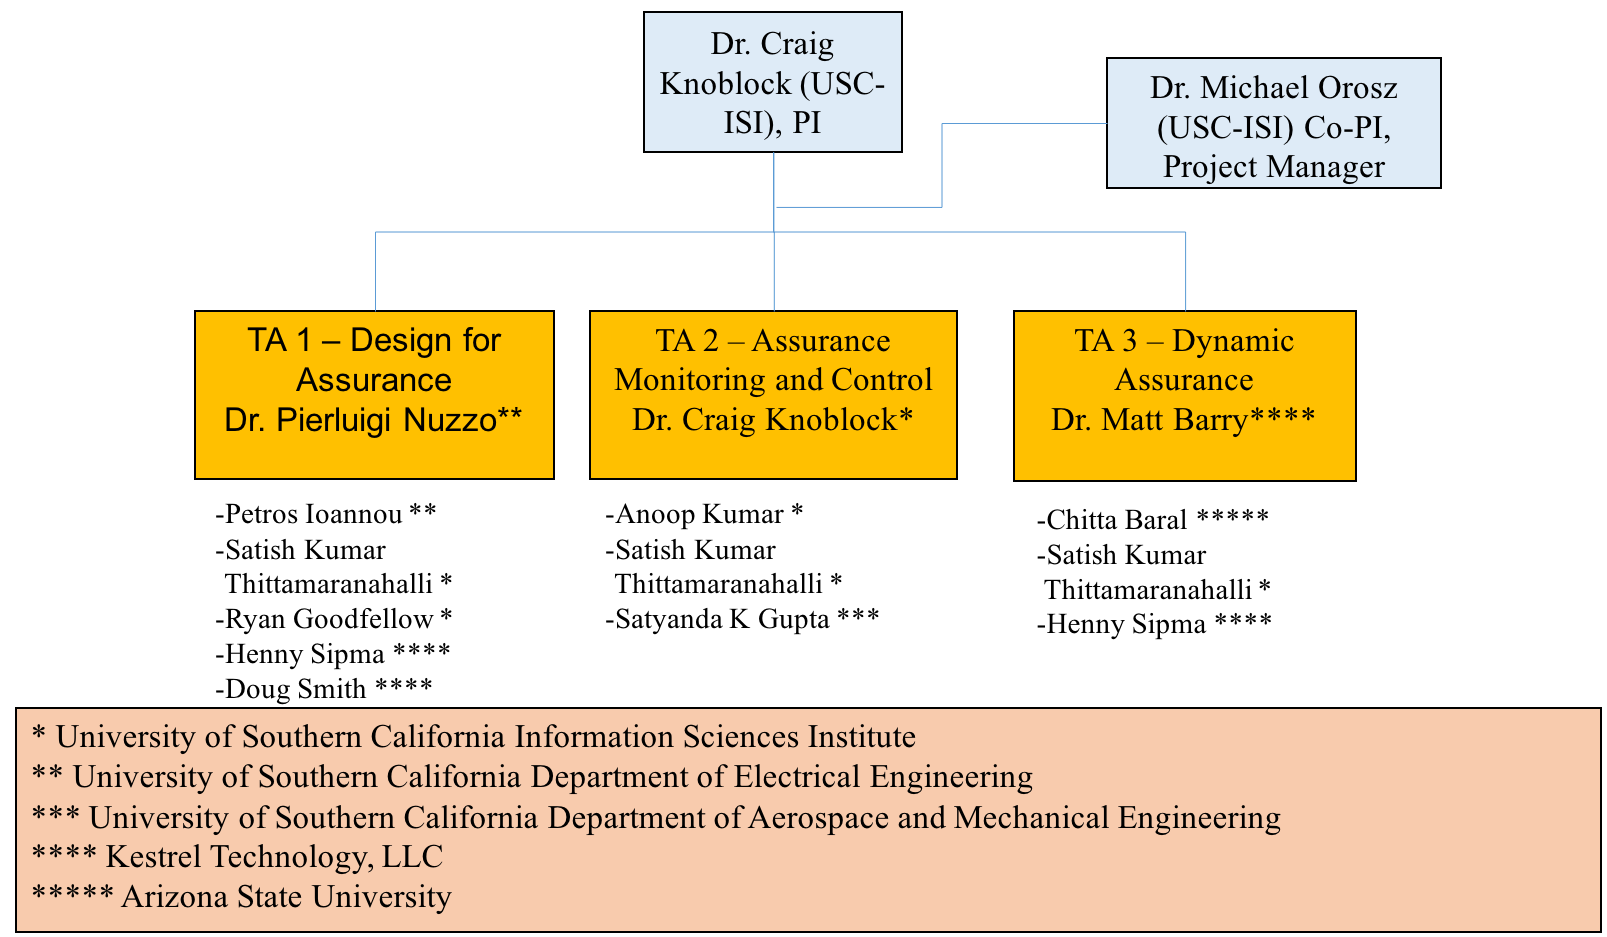
\includegraphics[width=6.0in]{./org-chart2.png}
\caption{\small Organization Chart}
\label{fig:org_chart}
\end{figure}

Coordination: To maximize collaboration and reduce risk to project failure from lack of communication and technical exchange, we plan to employ a wide variety of working styles and communication/coordination so that all can contribute.  At the core of our project will be regularly scheduled meetings bridging the diversely distributed team (Table~\ref{fig:Collaboration_Table}).  These meetings will address project status, identify challenges, implement risk mitigation strategies and participate in technology exchanges and system integration efforts (when appropriate)

\begin{table}[ht]
\caption{\small Project Meetings and Events}
  \centering
  {\footnotesize
\begin{tabular}{|m{3.15in}|m{3in}|} 
\hline
\textbf{Meeting} & \textbf{Frequency} 
\\\hline
Conference calls among investigators (discuss project status, address concerns and project risks) & Weekly
\\
\hline
Technical exchange and coordination meetings using Bluejeans or another videoconference technology & At least twice a month and more frequently as needed
  \\ 
\hline
Face-to-Face meetings (prior to P/I and demonstration meetings) & Every 3 to 6 months and more frequently (especially at the beginning of the project) as needed
 \\\cline{1-2}

\hline
\end{tabular}
}
\label{fig:Collaboration_Table}
\end{table}

\begin{table}[tbhp]
\caption{\small Key Project Team Member Responsibilities}
  \centering
  {\footnotesize
\begin{tabular}{| m{.75in} | m{3.9in}| m{1.5in}|} 
\hline
\textbf{Key Member} & \textbf{Responsibilities} & \textbf{Tasks} 
\\\hline
Dr.\ Craig Knoblock  & Principal Investigator responsible for project, leads TA 2 – Assurance Monitoring and Control.  Will lead the overall project and lead the TA2 team.  Served as the PI on many DARPA projects and has sucessfully led many large teams.    Effort on project:  25\% &
1.1.6, 1.2.2 1.2.3, 1.2.4, 1.3.4, 1.4.1, 
2.1.6, 2.2.2 2.2.3, 2.2.4, 2.3.4, 2.4.1, 
3.1.6, 3.2.2, 3.2.3, 3.2.4, 3.3.4, 3.4.1
\\
\hline
Dr.\ Michael Orosz & Co-Principal Investigator responsible managing the day-to-day operations of the project, assist technical teams as needed, coordinate with TA4 teams.    Has led many large complex multi-disciplined/multi-organizational projects in academic and industry environments.  Effort on project: 50\%
& 1.1.6, 2.1.6, 3.1.6, 1.4.1, 2.4.1, 3.4.1
  \\ 
\hline
Dr.\ Pierluigi Nuzzo 
& 
Co-Principal Investigator.  Leads the TA 1 - Design for Assurance team and conducts research on the formal methods for the design of the TA1 system.  Research experience on methodologies and tools for the design of cyber-physical systems; contracts, interfaces, and compositional methods for embedded system design; the application of automated formal methods and optimization theory to problems in embedded and cyber-physical systems.  Effort on project: 2 months/year (16.6\%)
& 
1.1.1, 2.1.1, 3.1.1 \\
\hline
Dr.\ Matthew Barry
& 
Key personnel.  Leads the TA 3 – Dynamic Assurance.   He will conduct the research on the dynamic assurance case language editors and parsers, the run-time system, and system integrations. Effort on project:  66\%
& 
1.3.2, 2.3.2, 3.3.2\\
\hline
Dr.\ Chitta Baral
& 
Key personnel responsible for learning assurance rules, supporting assurance rules with uncertainty and improving solver speed.  Expertise on ASP solvers, which will be used to reason about the assurance cases. Effort on project: 20\%
& 
1.3.1, 2.3.1, 3.3.1 \\
\hline
Dr.\ Doug Smith 
& 
Key personnel will support formal methods aspects of TA1, and lead the effort on abstract refinement. Expertise in field of automated correct-by-construction program generation.    Effort on project: 40\%
& 
1.1.5, 2.1.5, 3.1.5 \\
\hline
Dr.\ Henny Sipma
& 
Key personnel who will support the program verification tasks under TA1.  Will lead the effort on program verification.   Effort on project:  45\%
& 
1.1.5, 2.1.5, 3.1.5, 1.3.2, 2.3.2, 3.3.2 \\
\hline
Dr.\ Petros Ioannou
& 
Key personnel responsible providing and extending the assurance test bed, which will be available at the start of the project for autonomous vehicles.   Effort on project: 1 month/year (8.3\%)
& 
1.1.2, 2.1.2 (optional), 3.1.2 (optional)
\\
\hline
Dr.\ Satyandra Kumar Gupta
& 
Key Personnel providing autonomous command and control expertise to the TA-2 team.   Will lead the research on safety aware learning on TA2.   Past research on physics-aware decision making to facilitate automation.  Effort on project: 1 month/year (8.3\%)
& 
1.2.1, 2.2.1, 3.2.1 \\
\hline
Dr.\ Anoop Kumar 
& 
Key personnel providing support to the TA 2 project team.  Will lead the research on monitoring \& control and detecting distribution shifts.  Effort on project: 50\%
& 
1.2.1, 1.2.2, 1.2.3, 1.2.4, 2.2.1, 2.2.2, 2.2.3, 2.2.4, 3.2.1, 3.2.2, 3.2.3, 3.2.4\\
\hline
Dr.\ Satish Thittamaranahalli
& 
Key personnel developing scalable algorithms for TA1, TA2, and TA3 project teams.  Has extensive experience on scalable algorithm design, machine learning, and constraint reasoning.  Effort on project: 50\%
& 
1.2.1, 1.2.2, 1.2.3, 1.2.4, 2.2.1, 2.2.2, 2.2.3, 2.2.4, 3.2.1, 3.2.2, 3.2.3, 3.2.4, 1.1.4, 2.1.4, 3.1.4 \\
\hline
Dr.\ Ryan Goodfellow
& 
Key personnel providing support to the TA-1 project. Will lead the research on simulation-based testing.  Has extensive experience on simulation-based testing.  Effort on project:  30\%
& 
1.1.3, 2.1.3, 3.1.3 \\

\cline{1-2}

\hline
\end{tabular}
}
\label{fig:Table_Mgmt}
\end{table}



\newpage
\section{Personnel, Qualifications and Commitment}

{\bf Dr.\ Craig Knoblock}, the PI on this effort, is a Research Professor of both Computer Science and Spatial Sciences at the University of Southern California (USC) and Director of the Intelligent Systems Division at the USC Information Sciences Institute.   He received his Ph.D. from Carnegie Mellon University in computer science. 
%His research focuses on techniques for describing, acquiring, and exploiting the semantics of data.  
In previous projects he has worked on developing  scalable approaches to execution monitoring, accurate detection of sensor failures, and   automatic modeling and reconstruction of sensors.  He has published more than 300 journal articles, book chapters, and conference papers on these topics.  Dr. Knoblock is a Fellow of the Association for the Advancement of Artificial Intelligence (AAAI), a Distinguished Scientist of the Association of Computing Machinery (ACM), a Senior Member of IEEE, past President and Trustee of the International Joint Conference on Artificial Intelligence.
%and winner of the 2014 Robert S. Engelmore Award.  

{\bf Dr.\ Michael Orosz}, a Co-PI on this effort, is a Research Associate Professor of Civil and Environmental Engineering at the University of Southern California (USC) and Research Director of the Decision Systems Group at the USC Information Sciences Institute.  Dr. Orosz has over 30 years’ experience in commercial and government software development, basic and applied research, project management, academic research and has developed and deployed several commercially successful products.  His research interests are in machine learning and decision analytics as applied to intelligence analysis and autonomous command and control such as smart building controls.    Dr. Orosz has extensive experience in managing large complex multi-disciplined/multi-teamed research projects. %funded by DARPA, DHS, DoD, DoE, Industry, NASA, NRO, NSA and ONR.   
He received his Ph.D. in computer science from the University of California, Los Angeles.

{\bf Dr.\ Pierluigi Nuzzo}, a Co-PI on this project, is an Assistant Professor in the Department of Electrical Engineering at the University of Southern California. He received the Ph.D. in Electrical Engineering and Computer Sciences from the University of California at Berkeley. 
%in 2015, and the Laurea degree (MS) in electrical engineering (summa cum laude) from the University of Pisa, Italy, and the Sant'Anna School of Advanced Studies, Pisa, Italy.
%
%He has four years of research experience in analog and mixed signal circuit design as a researcher at IMEC, Leuven, Belgium, and over 10 years experience in design methodologies and tools for mixed-signal integrated circuits and cyber-physical systems, as a researcher at the University of Pisa, IMEC, UC Berkeley, and USC. 
His research interests
include: methodologies and tools for cyber-physical system and mixed-signal
system design; contracts, interfaces and compositional methods for embedded
system design; the application of formal methods and optimization theory to problems in embedded and cyber-physical systems and electronic design automation. 
%
Prof. Nuzzo received %First Place in the operational category and Best Overall
%Submission in the 2006 DAC/ISSCC Design Competition, 
a Marie Curie Fellowship
from the European Union in 2006, 
the University of California at Berkeley EECS
departmental fellowship in 2008, 
%the University of California at Berkeley Outstanding Graduate Student Instructor Award in 2013, 
the IBM Ph.D.
Fellowship in 2012 and 2014, 
%the Best Paper Award from the International Conference on Cyber-Physical Systems (ICCPS) in 2016, 
and the David J.~Sakrison Memorial Prize in 2016 for his doctoral research. 
%He is an author of 1 patent and over 60 publications.

{\bf Dr.\ Satyandra K. Gupta} is Smith International Professor in the Department of Aerospace and Mechanical Engineering at the University of Southern California. %Prior to joining the University of Southern California, he was a Professor in the Department of Mechanical Engineering and the Institute for Systems Research at the University of Maryland. He was the founding director of the Maryland Robotics Center and the Advanced Manufacturing Laboratory at the University of Maryland. 
He served as a program director for the National Robotics Initiative at the National Science Foundation from September 2012 to September 2014.  Dr. Gupta's interest is in the area of physics-aware decision making to facilitate automation. He has published more than 300 technical articles. He is a fellow of the American Society of Mechanical Engineers (ASME) and editor of ASME Journal of Computing and Information Science in Engineering. Dr. Gupta has received the Young Investigator Award from the Office of Naval Research in 2000, CAREER Award from the National Science Foundation in 2001, Presidential Early Career Award for Scientists and Engineers (PECASE) in 2001, Invention of the Year Award at the University of Maryland in 2007, Kos Ishii-Toshiba Award from ASME in 2011, and Excellence in Research Award from ASME in 2013.%, and Distinguished Alumnus Award from Indian Institute of Technology, Roorkee in 2014. %He has also received seven best paper awards at conferences.

{\bf Ryan Goodfellow} is a computer scientist at ISI working in combined cyber physical simulation and emulation platform development. His formal background is in simulation algorithms and modeling techniques using differential-algebraic equations (DAE). He has applied this knowledge in the CPS space by integrating DAE modeling languages and simulation engines with network testbeds to create comprehensive scientific experimentation platforms for cyber-physical systems. These experimentation platforms have been used in the power grid research space. %Ryan is a lead developer on the Deter network testbed, with a strong background in networked and distributed systems engineering. %He is also a combat veteran, serving as a non-commissioned officer and SIGINT team lead for a multi-functional intelligence team in Afghanistan.

{\bf Dr.\ Petros Ioannou} is a Professor in the Department of Electrical Engineering, Director of the Center for Advanced Transportation Technologies and Associate Director for Research for the DOT supported University Transportation Center at USC. He received his MS and PhD from the University of Illinois at Urbana Champaign in Mechanical and Electrical Engineering, respectively. His research interests are in robust adaptive control, vehicle dynamics and control, human factors and safety, automated vehicles, nonlinear systems and Intelligent transportation Systems.  He received the 2016 IEEE Transportation Technologies field award and the 2016 IEEE Control system society Transition to Practice Award. He is a Fellow of IEEE, IFAC and IET and author/coauthor of 8 books and over 400 papers.

{\bf Dr.\ Matthew Barry} will serve as lead for the TA3 tasks. %He will implement the dynamic assurance case language editors and parsers, the run-time system, and system integrations.  He will implement the assurance case arguments and the API for updating argument structure and content.  
Dr. Barry currently is CEO at Kestrel Technology LLC, and previously spent 20 years in NASA space mission operations at the Jet Propulsion Lab and Johnson Space Center.  At NASA Headquarters he led the introduction of dependability case requirements and plans for flight computing systems in upcoming manned space exploration missions, as well as the development of Agency-level software-related safety-critical control system requirements.  He recently served as a Principal Investigator on DHS/Cyber S\&T STAMP (Static Tool Analysis Modernization Program), DARPA CSFV (Crowd Sourced Formal Verification), three NASA Aeronautics R\&D projects, and the AFRL-sponsored Static Analysis of Numerical Algorithms project.  Dr. Barry earned BSME, MS, and PhD degrees in mechanical engineering, and an MBA degree, from Rice University.  

{\bf Dr.\ Henny Sipma} will support the program verification tasks under TA1.  %She is the key person behind the company's {\em KT Advance\/} and {\em KT Transferal\/} static analysis products, and the designer and programmer of the company's core {\em CodeHawk\/} abstract interpretation engine. 
Dr. Sipma currently is the CTO at Kestrel Technology LLC.  She has spent the past 10 years with Kestrel Technology as a static analysis expert; previously developed and taught static analysis techniques as senior research associate at Stanford University for eight years; and developed industrial process controls as an senior systems analyst at Shell.  She has been Principal Investigator or company lead on several recent R\&D projects for Federal agencies, including two projects under the IARPA STONESOUP (Securely Taking On New Executable Software of Uncertain Provenance) program; the DHS Cyber S\&T Gold Standard project; and the DARPA-sponsored STAC (Space-Time Analysis for Cybersecurity) and MUSE (Mining and Understanding Software Enclaves) programs.  Dr. Sipma earned 
%a BS degree in chemistry and an MS degree in chemical engineering at the University of Groningen in The Netherlands, and 
MS and PhD degrees in computer science from Stanford University.  

{\bf Dr.\ Douglas R.\ Smith} will support formal methods aspects of TA1, including the enforcement of safety properties and the generation of monitors.  He is President of Kestrel Technology LLC and Principal Scientist at Kestrel Institute.  He is a Fellow of the American Association of Artificial Intelligence (AAAI) and an ASE Fellow (Automated Software Engineering).  From 1986 to 2000, he taught an advanced graduate course on correct-by-construction software development at Stanford.  
%Dr. Smith has led the development of a series of software synthesis systems, including KIDS (Kestrel Interactive Development System), Specware, Designware, and Planware. 
%Applications domains have included a variety of complex high-performance planners and schedulers for the US Air Force.  He leads current projects on the generation of air mission plans and cyberoperations.  
Other recent projects focused on automated policy enforcement \cite{SmithD0703,SmithD08}, synthesis of secure network protocol codes, and the synthesis of high-performance constraint-solvers\cite{SmithD08c,SmithD13}.  Dr. Smith has over 30 years experience in the field of automated correct-by-construction program generation and has published over 100 papers. He has one patent.  He received the Ph.D. in Computer Science from Duke University% in 1979.  

{\bf Dr. Chitta Baral} is a Professor in the Department of Computer Science and Engineering at Arizona State University. He will support the TA3 efforts on Learning assurance rules, supporting assurance rules with uncertainty and improving solver speed. Dr. Baral has expertise in various aspects of autonomy and Artificial Intelligence. 
He wrote the first book on answer set programming (published by Cambridge University Press) the formal language behind our assurance rules. Some of his other works relevant to this proposal are: goal specification for autonomous systems, automatic construction of control rules for autonomous systems that satisfy given goals, combining machine learning with reasoning in various contexts, including image understanding. %He is the President of KR Inc. He is an associate editor of AIJ and has been an associate editor of JAIR.

{\bf Dr.\ Satish Kumar Thittamaranahalli (T. K. Satish Kumar)} leads the Collaboratory for Algorithmic Techniques and Artificial Intelligence (CATAI) at USC's Information Sciences Institute. He has published over 60 papers on numerous topics in Artificial Intelligence spanning such diverse areas as Constraint Reasoning, Planning and Scheduling, Probabilistic Reasoning, Robotics, Combinatorial Optimization, Approximation and Randomization, Heuristic Search, Model-Based Reasoning, Knowledge Representation and Spatio-Temporal Reasoning. %He %has served on the Program Committees of many international conferences in Artificial Intelligence
He and is a winner of the 2016 Best Robotics Paper Award and the 2005 Best Student Paper Award from the International Conference on Automated Planning and Scheduling. 
Dr. Kumar received his PhD in Computer Science from Stanford University. %In the past, he has also been a Visiting Student at the NASA Ames Research Center, a Postdoctoral Research Scholar at the University of California, Berkeley, a Research Scientist at the Institute for Human and Machine Cognition, a Visiting Assistant Professor at the University of West Florida, and a Senior Research and Development Scientist at Mission Critical Technologies.

\textbf{Dr.\ Anoop Kumar} is a senior computer scientist at USC ISI and has broad expertise in machine learning, statistical modeling, and software engineering.  Dr.\ Kumar is the technical lead on the DARPA RSPACE program and has played a vital role in developing a system that fuses air operations data from multiple sources, maintains world state, and issues warnings. Previously, he led the research and development of the BBN’s election forecasting system for the IARPA OSI program. %Dr.\ Kumar played a significant role in the DARPA DEFT program by developing a model to support integration of output from multiple NLP algorithms. He has contributed at the development to management levels on government research contracts and commercial projects. 
Dr.\ Kumar helped design and develop BBN's commercially available, hosted speech and medical transcription services offering. 

\begin{table}[!tbh]
\begin{footnotesize}
\vspace{-0.1in}

\begin{tabular}{lll}
\begin{tabular}[t]{|l|@{}c@{}|@{}c@{}|@{}c@{}|@{}c@{}|} \hline
Project & Status & \multicolumn{3}{ c| }{Hours} \\ \cline{3-5}
& & P1 & P2 & P3 \\ \hline



\multicolumn{5}{ |c| }{ \textbf{Craig Knoblock} } \\ \cline{1-5}
Safeguard & Pro & 770 & 641 & 641 \\ \cline{1-5}
ELICIT & Cur & 308 & 256 & 120 \\ \cline{1-5}
WTNIC & Cur & 11 & 0 & 0 \\ \cline{1-5}
EFFECT & Cur & 641 & 107 & 0 \\ \cline{1-5}
LinkedMaps & Cur & 203 & 25 & 0 \\ \cline{1-5}
PRINCESS & Cur & 608 & 96 & 0 \\ \cline{1-5}
SCHARP & Cur & 481 & 54 & 0 \\ \cline{1-5}
MINT & Pen & 650 & 534 & 285 \\ \cline{1-5}

\multicolumn{5}{ |c| }{ \textbf{Michael Orosz} } \\ \cline{1-5}
Safeguard & Pro & 1560 & 1300 & 1300  \\ \cline{1-5}
SMC/SY & Cur & 1803 & 0 & 0  \\ \cline{1-5}

\multicolumn{5}{ |c| }{ \textbf{Matthew Barry} } \\ \cline{1-5}
Safeguard & Pro & 2078 & 1690 & 1554 \\ \cline{1-5}
Starlite & Cur & 1840 & 1692 & 0 \\ \cline{1-5}



\multicolumn{5}{ |c| }{ \textbf{Anoop Kumar} } \\ \cline{1-5}
Safeguard & Pro & 1560 & 1300 & 1300 \\ \cline{1-5}

\end{tabular}
&
\begin{tabular}[t]{|l|@{}c@{}|@{}c@{}|@{}c@{}|@{}c@{}|} \hline
Project & Status & \multicolumn{3}{ c| }{Hours} \\ \cline{3-5}
& & P1 & P2 & P3 \\ \hline

\multicolumn{5}{ |c| }{ \textbf{Pierluigi Nuzzo} } \\ \cline{1-5}
Safeguard & Pro & 520 & 433 & 433  \\ \cline{1-5}
Mirage & Cur & 433 & 0 & 0  \\ \cline{1-5}

\multicolumn{5}{ |c| }{ \textbf{Satyandra Gupta} } \\ \cline{1-5}
Safeguard & Pro & 260 & 217 & 217 \\ \cline{1-5}
Human   & Cur & 22 & 0 & 0 \\ \cline{1-5}
Vehicles & Cur & 36 & 0 & 0 \\ \cline{1-5}
Robot & Cur & 116 & 0 & 0 \\ \cline{1-5}
Assembly & Cur & 33 & 0 & 0 \\ \cline{1-5}
Solar & Cur & 4 & 0 & 0 \\ \cline{1-5}

\multicolumn{5}{ |c| }{ \textbf{Petros Ioannou} } \\ \cline{1-5}
Safeguard & Pro & 260 & 217 & 217 \\ \cline{1-5}
CPS & Cur & 130 & 0 & 0 \\ \cline{1-5}

\multicolumn{5}{ |c| }{ \textbf{Ryan Goodfellow} } \\ \cline{1-5}
Safeguard & Pro & 936 & 780 & 780 \\ \cline{1-5}
STEAM & Cur & 416 & 0 & 0 \\ \cline{1-5}


\end{tabular}
&
\begin{tabular}[t]{|l|@{}c@{}|@{}c@{}|@{}c@{}|@{}c@{}|} \hline
Project & Status & \multicolumn{3}{ c| }{Hours} \\ \cline{3-5}
& & P1 & P2 & P3 \\ \hline

\multicolumn{5}{ |c| }{ \textbf{Chitta Baral} } \\ \cline{1-5}
Safeguard & Pro & 659 & 485 & 485 \\ \cline{1-5}
PostdocBP & Cur & 176 & 0 & 0 \\ \cline{1-5}
Languages & Pen & 528 & 264 & 264 \\ \cline{1-5}
CAREER & Pen & 88 & 44 & 44 \\ \cline{1-5}
CHS & Pen & 510 & 255 & 0 \\ \cline{1-5}

\multicolumn{5}{ |c| }{ \textbf{Doug Smith} } \\ \cline{1-5}
Safeguard & Pro & 1222 & 984 & 840 \\ \cline{1-5}
RSPACE & Cur & 342 & 0 & 0 \\ 
\cline{1-5}
PLANX & Cur & 154 & 0 & 0 \\ 
\cline{1-5}
HACCS & Pen & 923 & 769 & 769 \\ 
\cline{1-5}

\multicolumn{5}{ |c| }{ \textbf{Henny Sipma} } \\ \cline{1-5}
Safeguard & Pro & 1372 & 962 & 840 \\ \cline{1-5}
STAC & Cur & 797 & 0 & 0 \\ \cline{1-5}

\multicolumn{5}{ |c| }{ \textbf{Satish Thittamaranahalli} } \\ \cline{1-5}
Safeguard & Pro & 1560 & 1300 & 1300 \\ \cline{1-5}
MapF & Cur & 103 & 103 & 0 \\ \cline{1-5}

\end{tabular}
\end{tabular}

\end{footnotesize}
\caption{Individual commitments of key personnel}
\label{tab:Commitments}
\vspace{-0.2in}
\end{table}

\clearpage
\newpage
\section{Capabilities}


%\subsection{University of Southern California}
USC has strengths in number of areas that are closely related to the proposed work:
\begin{itemize}[itemsep=0pt,leftmargin=*]
\item Dr.\ Nuzzo 
%has over 10-year research experience in embedded system design, from mixed-signal chip design (analog-to-digital converters, frequency synthesizers, software-defined radio), to methodologies and tools for mixed-signal integrated circuits and Cyber-Physical Systems (CPSs), and the application of formal methods and optimization theory to problems in embedded and cyber-physical systems and electronic design automation.  
%His doctoral work 
has done extensive research on contracts and compositional methods for heterogeneous system design and design space exploration, with application to aircraft electric power systems and environmental control systems. His work has helped transition rigorous system design foundations, innovative design methodologies, and new systems engineering paradigms to industry (IBM, United Technologies). 
\item Dr.\ Satyandra K. Gupta has worked on autonomous surface vehicles, autonomous ground vehicles for operation on rugged terrains, and autonomous flapping wing aerial vehicles.   His group has developed a hierarchal decision making approach for realizing autonomous systems. 
%This approach combines task planning and assignment, deliberative trajectory planning, reactive collision avoidance behaviors, and trajectory tracking control layers. 
His group has also developed new methods for learning reactive behaviors in adversarial environments and COLREGS compliant trajectory planning. \item Dr.\ Knoblock has developed methods that learn the relationships between sensors to both identify failures and changes in sensor and reconstruct those sensors, providing estimates of the accuracy of the reconstructed sensors.  
\item Ryan Goodfellow has extensive experience in simulation based testing through high-fidelity CPS testbed environment development and operation, using the Deter network testbed as the core which has supported several large scale government projects from a variety of agencies and thousands of users. %we have developed sophisticated CPS experiments under programs such as NFS RIPS, NIST SmartCities and the DHS Cybersecurity showcase.
\item Dr.\ Ioannou %helped  design and implement adaptive cruise control systems in collaboration with Ford Motor Company, which was commercialized four years before any other company. He 
worked on several DOT funded projects on automated vehicles and intelligent highway systems where he demonstrated his vehicle control designs for safety and performance on actual automated vehicles in test trucks and I-15 highway.
\item Drs.\ Knoblock, Kumar, and Thittamaranahalli have developed highly scalable approaches for monitoring message traffic to identify potential problems and issue warnings and alerts. 
\item Dr. Thittamaranahalli has developed state-of-the-art methods for efficiently solving large-scale search and optimization problems. %These techniques will be applicable in TA2 for safety-aware learning and planning, in TA2 for assurance monitoring and control, and in TA3 for dynamic assessment of assurance cases.

\end{itemize}
%\subsection{Kestrel Technology LLC}

Kestrel Technology's strength is in program analysis, specifically static analysis of both source and binary targets.  The company performs applied R\&D and product development for a variety of static analysis applications  pivoting primarily on the abstract interpretation technique.  The company recently initiated development of program analysis applications using logical equivalence techniques. As a provider of verification evidence in the form of mathematical proofs, the company also has expertise in the design and development of assurance case arguments for high-integrity systems using such evidence. %The company is engaged in a partnership with Wind River Systems to develop program analysis tools for its embedded system developers.  Many of Wind River's customers must develop their products under safety and certification standards, including those using safety cases.  

   

%\subsection{Arizona State University}
Chitta Baral at Arizona State University has developed various software to learn assurance rules and various ASP solvers, which he has made available as open-source.

Most of the software carried forward for implementation or derivation is open source.  The single exception is Kestrel Technology's {\it KT Advance\/} static analysis tool (TA1), in particular the abstract interpretation engine therein, which is company proprietary and is US EAR export-controlled.   
%Owing to mixed funding for the development of that technology 
We will continue to provide the Federal government a restricted use license for that particular item.

There are no specialized facilities, data, or GFE required for this effort. 

\include{sow}
\include{milestones}

% \section{Level of Effort by Task \textcolor{red}{[Mike/Lisa - 1 pages]}}

% \textcolor{blue}{
% \begin{itemize}
% \item Will be a separate spreadsheet
% \item
% \end{itemize}
% }

\include{appendix_a}

%\section{Appendix B \textcolor{red}{[No Page Count]}}

\section{References}
\bibliographystyle{acm} 
\bibliography{TA3/ta3,TA2/ta2,TA1/ta1}
\end{document}
%%\documentclass[a4paper]{article}
%\documentclass[12pt]{article}
\documentclass[12pt]{dod-blank}

%% Language and font encodings
\usepackage[english]{babel}
\usepackage[utf8x]{inputenc}
\usepackage[T1]{fontenc}

%% Sets page size and margins
%%\usepackage[a4paper,top=3cm,bottom=2cm,left=3cm,right=3cm,marginparwidth=1.75cm]{geometry}
%\usepackage[top=1in, bottom=1in, left=1in, right=1in]{geometry}



%% Useful packages
\usepackage{amsmath}
\usepackage{graphicx}
  \graphicspath{{.}{./image/}}
  \DeclareGraphicsExtensions{.png,.jpg} 
\usepackage[colorinlistoftodos]{todonotes}
\usepackage[colorlinks=true, allcolors=blue]{hyperref}
\usepackage{tabularx}
\usepackage{multirow}
\usepackage{tabulary}
\usepackage{float}
\usepackage{wrapfig}
\usepackage[export]{adjustbox}
\usepackage{comment}
\usepackage{tabularx}
\usepackage{multirow}
\usepackage{tabulary}
\usepackage{enumitem}

\usepackage{listings}
\usepackage{color}
\usepackage{array}
\usepackage{subcaption}
\usepackage{xcolor}




\renewcommand{\textfraction}{0}
\renewcommand{\topfraction}{1.0}
\renewcommand{\bottomfraction}{1.0}

\usepackage{longtable}
%% macros
\newif\iffinal
\finaltrue
\iffinal
  
    \newcommand\baareq[1]{}
    \newcommand\baades[1]{}
 
 
\else
    \definecolor{darkgreen}{rgb}{0,0.4,0}
    \definecolor{darkcyan}{rgb}{0,0.4,0.4}
    \definecolor{darkblue}{rgb}{0,0,0.5}
    
    \newcommand\baareq[1]{{\color{darkcyan}[\textbf{Requirement:} #1]}}
    \newcommand\baades[1]{{\color{darkcyan}[\textbf{Description:} #1]}}
 
\fi




\def\naive{na\"{\i}ve}



\lstset{ 
  backgroundcolor=\color{white},   % choose the background color; you must add \usepackage{color} or \usepackage{xcolor}
  basicstyle=\footnotesize\ttfamily,            % the size of the fonts that are used for the code
  breakatwhitespace=false,         % sets if automatic breaks should only happen at whitespace
  breaklines=true,                 % sets automatic line breaking
  captionpos=b,                    % sets the caption-position to bottom
  commentstyle=\color{mygreen},    % comment style
  % deletekeywords={...},            % if you want to delete keywords from the given language
  escapeinside={\%*}{*)},          % if you want to add LaTeX within your code
  extendedchars=true,              % lets you use non-ASCII characters; for 8-bits encodings only, does not work with UTF-8
  frame=single,	                   % adds a frame around the code
  keepspaces=false,                 % keeps spaces in text, useful for keeping indentation of code (possibly needs columns=flexible)
  keywordstyle=\color{blue}\bfseries\underbar,       % keyword style
  language=Prolog,                 % the language of the code
  % morekeywords={if,and},        % if you want to add more keywords to the set
  numbers=none,                    % where to put the line-numbers; possible values are (none, left, right)
  numbersep=5pt,                   % how far the line-numbers are from the code
  numberstyle=\tiny\color{mygray}, % the style that is used for the line-numbers
  rulecolor=\color{black},         % if not set, the frame-color may be changed on line-breaks within not-black text
  showspaces=false,                % show spaces everywhere adding particular underscores; it overrides 'showstringspaces'
  showstringspaces=false,          % underline spaces within strings only
  showtabs=false,                  % show tabs within strings adding particular underscores
  stepnumber=2,                    % the step between two line-numbers. If it's 1, each line will be numbered
  stringstyle=\color{mymauve},     % string literal style
  tabsize=2,	                   % sets default tabsize to 2 spaces
  title=\lstname                   % show the filename of files included with \lstinputlisting; also try caption instead of title
}

% apply trick for additional keywords for our AC DSL
\lstset{
	emph={for, if, and, or},
    emphstyle={\color{blue}\bfseries\underbar}
}




\title{DARPA Assured Autonomy}
\author{Technical Volume- \textcolor{red}{Thirty-Eight (38) pages max}}

\begin{document}
\pagenumbering{roman}
\include{cover}

\newpage
\section{Table of Contents}
\tableofcontents

\newpage
\pagenumbering{arabic}
\section{Executive Summary}
As we rapidly move into a world where machine learning plays a central role in realizing autonomous systems, it is becoming increasingly important to develop techniques that assure that these systems will operate safely and perform as expected. Current approaches are limited to providing assurance for systems with limited or no  learning capabilities. In this context, DARPA's Assured Autonomy BAA seeks to \emph{develop rigorous design and analysis technologies for continual assurance of learning-enabled autonomous systems}. USC in collaboration with Kestrel Technology and ASU is pleased to submit a comprehensive TA1, TA2, and TA3 proposal entitled \emph{``Assured Autonomy for Learning Enabled Vehicles (Safeguard).''} We plan to provide an end-to-end solution to support autonomous systems with learning-enabled components, ranging from design technologies for assurance, to assurance monitoring and control techniques, to representation and online evaluation of assurance cases. We have assembled a strong team of experts that cover the range of technologies that are required to create such an end-to-end system. If successful, the project will provide the technologies for building the next-generation of learning-enabled autonomous systems.  The entire project will take four years and cost \textcolor{red}{\$??}, with an initial version completed at the end of Phase I and successive versions with additional capabilities and improved scalability at the end of Phase II and Phase III.  

In the remainder of this section, we first introduce an  unmanned surface vehicle scenario that will be used throughout the proposal to describe the approach.  Next, we describe our approach to design, monitoring, and dynamic assurance. Finally, we introduce the team involved in the project. 

\textbf{Motivating Scenario.} Consider an autonomous unmanned surface vehicle (USV) guarding a valuable asset in the ocean when an unknown vehicle  approaches the security perimeter, under challenging weather conditions. In this scenario, the USV is required to approach the intruding vehicle, issue a warning signal, and escort it to a safe distance from the controlled area. However, as the USV has no a priori knowledge of its external environment behaviors (e.g., water depth, waves, wind, current, visibility), pre-computing a feasible trajectory, let alone optimal, becomes a non-trivial problem. For trajectory planning, the USV must continuously perform the following tasks:
\begin{itemize}[itemsep=0pt,leftmargin=*]
 \item Sense the current state of the surrounding environment (e.g., water depth, waves, wind, current, visibility) and estimate its own maneuverability constraints (e.g., braking distance, available acceleration, maximum velocity, turning radius, turning rate, safety distance) based on the state of the environment;      
\item Sense the static obstacles in the sensor range and generate a traversability map;
\item Sense the moving obstacles and classify them;   
\item Predict future trajectories of moving obstacles; 
\item Determine if any of the COLREGS \cite{commandant1999international} rules will be in effect with respect to one or more of the nearby vessels and identify the vessels with the right of way.    
\end{itemize}
The above information will be used by the trajectory planner to compute an initial trajectory, which will be continuously refined as the USV gathers additional information.
% It is not possible for the USV to be tested in every possible environment. 
The USV will use learning enabled components to take  decisions as it encounters new situations, such as  
\begin{itemize}[itemsep=0pt,leftmargin=*]
\item Classifiers to identify moving obstacles based on physical appearance and motion signatures,
\item Algorithms to estimate the sensor capabilities in adverse weather conditions,   
\item Algorithms to accurately estimate uncertainty in the environment, 
\item Classifiers to generate traversability maps,
\item Prediction of external vessel behaviors based on motion histories, 
\item Reinforcement learning  to ensure COLREGS compliance of maneuvers,  
\item Algorithms to learning pursuit behaviors.  
\end{itemize}
Learning enabled components will interact with each other in complex ways, where a misclassification error in one component may eventually compromise the entire mission.   
% We will need to make sure that each learning enabled components has a run-time monitor that will ensure that the assumptions made by the learning-enabled component remain valid and prevent erroneous learning. 
% For example, if the vehicle is exhibiting significant error in trajectory tracking, then simply downgrading the trajectory tracking error value may not be a good option.  The failure of prediction of trajectory tracking error might be due to the presence of a significant wake caused by a nearby vessel. The presence of the nearby vessel can be used to explain the degradation in trajectory tracking performance. As the vessel moves away, we can expect the trajectory tracking performance to return to the predicted level.  
While exhaustive validation of learning-enabled cyber-physical systems (LE-CPSs) is a prohibitive task~\cite{Kalra16},
their complexity, heterogeneity, and highly dynamic nature
make it challenging to even leverage existing model-based development techniques to effectively assess system correctness 
% dependability, 
at design time or enforce it at runtime.

\textbf{Design for Assurance.} Safeguard uses a platform-based design approach~\cite{Nuzzo15b} to organize the design process for a LE-CPS and to build assurance cases. Composite models are developed at several levels of abstraction,
from top-level system requirements and safety constraints down to the
implementation level.  Intermediate levels add detail to the levels
above.  The different levels are connected by refinement mappings that
allow properties established at one level to be preserved at the next
level (see Figures~\ref{fig:methodology} and~\ref{fig:assurance}).

Contracts are used to formally specify components and composite models
in terms of (1) Assumptions -- the assumed behaviors of the
environment and the behaviors of other components, and (2) Guarantees
-- the behavior properties that a model guarantees if it operates in a
context that satisfies its assumptions.  A calculus of contracts
allows horizontal composition of contracts to generate contracts for
composite models.  Vertical contracts are used to specify the mapping
or refinement relation between models at different levels of
abstraction.  The system design process starts with a high-level
contract that expresses overall system assumptions and requirements.
Subsequent levels express models with increasing detail until the
lowest level expresses the system in terms of hardware components and
their software controllers.

The assurance case for a CPS arises from the horizontal and vertical
structure of the design in several ways.  The components used within a
particular level are either (1) synthesized using
correct-by-construction design tools together with proofs, (2) derived
statically or dynamically using safety-aware machine-learning
techniques, (3) written manually and verified by analysis tools, or
(4) written manually and validated by extensive testing.  The
assurance case for the whole reflects its compositional structure.  We
anticipate that well-specified contracts together with the calculus of
contracts will eliminate well-known problems with unexpected emergent
behaviors in CPS systems.

The assurance case for the lowest-layer design arises from both the
intra-level assurance and from properties and their proofs that are
preserved under the refinement mapping from the top-level
requirements.  The refinement mappings between model layers will be
constructed using a variety of techniques.  A contract at an abstract
level can be mapped to a component or refined contract by (1)
retrieval of pre-verified components from a platform library, (2)
synthesis using correct-by-construction design and optimization tools,
or (3) manual coding to satisfy a contract.  The mapping of a
composite model will be composed from the mappings of its constituent
components or contracts.  When a composite model cannot be mapped
compositionally to the next level, it will be generated using
correct-by-construction design and optimization tools.

\textbf{Assurance Monitoring and Control.}
We provide an integrated framework for safety-aware learning, assurance monitoring and control, detecting distribution shifts. Three major components offer an efficient TA2 architecture as well as interfaces with TA1 and TA3, that is, (a) safety-aware learning and planning, (b) assurance monitors for guarding architectural and safety constraints; and (c) distribution shift detection.

We will develop a new learning-enabled online decision-making framework that allows opportunistically composing a sequence of actions (maneuvers) to reduce uncertainty in the system capability model without suspending the progress toward the mission goals or compromising safety. Each candidate action is evaluated based on three criteria: (1) the risk of violating a safety constraint using the current uncertainties in the parameter estimates; (2) its relevance to the mission goals; (3)  its expected information gain, i.e., reduction in uncertainty, with respect to the parameter estimates. These evaluations are combined to produce a cumulative mission utility value for each action that drives our learning-enabled decision-making framework. The problem of generating and evaluating sequences of actions can be posed in several way. For example, it can be solved using a branch-and-bound search method like Anytime A*, or formulated with the finite-horizon Markov Decision Process (MDP) framework. We will develop new scalable search strategies to solve this problem efficiently, by potentially evaluating a recent method developed at USC, called FastMap, that can significantly improve the execution time. 

We will develop monitors for architectural and safety constraints. 
% While these constraints can be checked over and over again as sensor information flow in, this naive strategy accounts for a lot of computational overhead. 
To achieve scalability and decrease the overhead, we propose the application of a technique that we currently use in DARPA's RSPACE program, which leverages a physical model of the vehicles dynamics and its interactions with the environment to efficiently determine the readout frequency. We propose two  extensions of this basic idea. First, we will use the theory of Variable Elimination to prioritize which variables to monitor, e.g., controllable, versus uncontrollable, adversarially controlled, or unobservable variables. Second, we invoke the dynamic assessment of assurance cases only when needed. This  decreases the number of times dynamic assessment of assurance cases is initiated as well as the communication bandwidth between the TA2 and TA3 components.

Finally, we will identify a distribution shift by combining statistical and machine learning techniques to differentiate between environmental and sensor changes. We will exploit a categorization of the shifts based on their cause and duration as well as extend our earlier work on detecting and mitigating sensor failures for all types of monitored variables.  

\textbf{Dynamic Assurance:} The Safeguard {\em design for assurance\/} activity takes a systems-theoretic stance toward safety.  Consequently, it presumes that safety is an emergent property of the system, and that hazards can present themselves through unintended interactions and performance violations in addition to causal events such as component failures.  Our design approach includes consideration of intent as well as hazard analysis and mitigation.  The artifacts from these activities populate contracts and assumptions for the dynamic assurance case.  
We thus build safety into the product by working at a systems-level viewpoint, using lexicon and design patterns familiar to both hardware and software engineers; safety is an emergent property of the system, not an afterthought.  
As system behavior evolves during runtime owing to learning, threats, degradation, or some other factor, the dynamic assurance case identifies whether the safety constraints continue to be satisfied.  If not, it provides notifications or issues recovery instructions directly from a lookup table.

Our implementation of the dynamic assurance case employs a declarative knowledge base inference engine and a domain-specific language tailored to our approach.  We have used them successfully for assurance case tool sets and arguments, and will extend them to reason about uncertainty and learning.  Our approach to achieve scalability is to specialize solvers toward modularity and to take advantage of domain knowledge.  Specifically, we will develop answer set programming techniques for context-dependent learning for reasoning about the learning-enabled components as well as learning assurance rules.  We will develop new formalisms for uncertainty to include causality, using weights for computing probabilities, and probabilistic non-monotonicity.  To achieve scaling objectives we will implement specializations using modularity, weighted CSPs, and message passing. 

% The system safety constraints revealed from that design become the key elements of our dynamic assurance case.  Our verification tools ensure the constraints are relevant, identifiable, and their implementation and effect observable.  

\textbf{Team.} We have assembled a team that is exceptionally well-qualified to build the proposed Safeguard system.  The team will be led by Dr.\ Craig Knoblock, the Principal Investigator for the effort, who currently leads the Intelligent Systems Division at the Information Sciences Institute.  He has led many large DARPA and IARPA projects over the years and has a strong track record in conducting leading edge research and then transitioning the technology to commercial use.  He will be supported by Dr.\ Michael Orosz as the Project Manager, who also has  experience in managing large research projects and on autonomous systems.  The TA1 team will be led by Dr.\ Pierluigi Nuzzo, who is an expert in embedded system design methodologies and the  application of formal methods to cyber-physical systems.  The TA1 team also includes Dr.\ Doug Smith, who has spent many years working on scalable correct-by-construction techniques and Dr.\ Henny Sipma, who has significant experience in applying program verification methods to real-world problems.  The TA1 team also includes Ryan Goodfellow, who has done a large amount of work on simulation-based testing.  The TA2 team will be led by Dr.\ Knoblock who has worked on topics related to both monitoring and detecting distribution changes.  He will be supported by Dr.\ Satyandra Gupta, who is an expert on autonomous surface vehicles as well as on safety-aware learning. He will also be supported by Drs.\ Anoop Kumar and Satish Thittamaranahalli, who have also previously worked on efficient methods for execution monitoring.  The TA3 team will be lead by Dr.\ Matthew Barry, who has experience in creating the technologies for assurance cases.  He will be supported by Dr.\ Chitta Baral, who is an expert on ASP solvers and by Dr.\ Thittamaranahalli who is an expert on SAT solvers, both of which will be applied to provide scalable assurance case reasoning.  Finally, Dr.\ Petros Ioannou, who is an expert on control systems for autonomous vehicles will provide an autonomous vehicle platform, which will form the focus of our work until the TA4 teams provide additional vehicle platforms for development.  

\newpage
\section{Innovative Claims and Deliverables}

In this project we will develop and build an end-to-end system for assured autonomy.  This section describes the key innovations by technical area and then the overall deliverables of the project.

\paragraph{Design for Assurance}

\begin{itemize}[itemsep=0pt,leftmargin=*]
\item We address the LE-CPS design challenges via a holistic approach that can contextually generate design artifacts and assurance cases. We develop a compositional, contract-based modeling framework, methods, and tools to support the design process from system-level requirement capture,  formalization, and analysis, to the generation, testing, and continual monitoring of software and hardware artifacts in feedback loop with a physical process.

\item We develop compositional abstractions and interfaces (vertical contracts) that can  bridge heterogeneous formalisms and heterogeneous decomposition architectures to make system analysis and synthesis tractable, consistently combine different verification and synthesis methods at design time, and provide seamless support for dynamic assurance at run time. %We aim to quantitatively capture the confidence in the satisfaction of requirements under uncertain or unknown conditions, and resilience properties of  systems at different abstraction levels, to enable trade-off evaluation between resilience, performance, and cost.

\item We develop a unifying framework and efficient algorithms to reason about the combination of discrete and continuous dynamics and constraints in the presence of uncertainties in LE-CPS using a satisfiability modulo convex approach~\cite{Shoukry2017} for contract-based system verification and scalable trajectory planning.  

\item We provide an environment for high-fidelity CPS testing, in which production-ready software, e.g.,  safety-critical learning and control, may be deployed and tested 
% by extending the Cypress testbed environment \cite{Goodfellow2015Cypress:Systems} 
with time dilation facilities, so that it synchronizes with a physical simulation that is not necessarily running in real time, while still having the perception of real time.

\item We 
% These facilities allow a cyber system to be  
propose an approach for unanticipated behavior space identification and test coverage maximization which leverages results from the theory of differential algebraic equation (DAE)~\cite{Berger2013ControllabilitySurvey,Ilchmann2005ATheory,BergerOnSystems,Lamour2013} 
to prune the behavior search space and identify smaller regions of interest for efficient simulation-based testing. 
% We then compute the intersection of these two behavior spaces and restrict our simulation based testing search space to this subspace.
\end{itemize}

\paragraph{Assurance Monitoring and Control}

\begin{itemize}[itemsep=0pt,leftmargin=*]
\item 
%We integrate safety-aware learning into the overall decision making problem. The goal is to maximize mission utility without violating the safety constraints. 
Our safety-aware learning framework enables the system to opportunistically select and execute actions to assist the learning-enabled component in reducing model uncertainty without compromising safety or deviating from the mission goals. The value of uncertainty reduction is explicitly incorporated in the optimization process for selecting the best action.  
\item For safety-aware learning, we propose the idea of preprocessing the search space of the problem domain before queries and observations come in. With such a linear-time preprocessing phase, the performance of search and optimization algorithms can be significantly boosted. For example, in regular A* search, the intensional or extensional search space can be preprocessed in near-linear time to yield an embedding of each state as a point in Euclidean space~\cite{cujakk}. Then, when the query comes in, A* search can make use of these Euclidean distances as heuristic distances between two states to yield order-of-magnitude speedups. 
%In Anytime A* for safety-aware learning and planning, this leads to a significantly better quality of actions chosen within a time limit, and in the MDP framework, the same ideas can be used to improve the convergence of Bellman updates for safety-aware Reinforcement Learning.
\item As massive amounts of sensor information flow in, it is imperative for us to efficiently process this information for monitoring architectural and safety constraints. Building on our past work on similar tasks, we propose novel technologies for efficiently monitoring constraints. These algorithms can yield an exponential reduction in the amount of sensor data that needs to be processed. Doing this also reduces the message complexities between the various modules. %We also propose to use the theory of Variable Elimination (VE) to monitor constraints with uncontrollable, adversarially controlled, and/or unobservable variables. VE yields a substrate constraint to monitor that characterizes a dominant strategy of the controllable variables over the uncontrollable, adversarially controlled, and/or unobservable variables.
\item We will develop techniques to identify  distributional shifts and determine the underlying cause (e.g., change in environment, sensor failure,   etc.), as well as strategies for handling the various distributional shifts.   Notably, we propose to build on our past work and use compact representations to exploit historical data to identify distributional shifts.
\end{itemize}

\paragraph{Dynamic Assurance}

\begin{itemize}[itemsep=0pt,leftmargin=*]

\item We demonstrate the integration of dynamic assurance for safety-critical learning-enabled dynamic systems in which evolutionary behaviors are expected and tolerated as a property of the functionality.   The impact will be consequential contributions safety-critical dynamic systems in which evolutionary behaviors are expected and tolerated as portion of the functionality.   
\item We implement dynamic assurance by combining features of system safety, formal methods, logic programming, uncertain reasoning, and domain-specific languages.  We populate assurance case arguments at several levels of modeling and implementation abstraction, using the analysis results to produce design-time evidence supporting assurance claims.  
%We provide automated reasoning about the assurance case itself to produce verification, consistency, and completeness results for the argument.  Dynamic assurance results then yield trusted explanations of whether safety constraints and assumptions and other contracts still hold during the collection of runtime evidence from monitors. 
\item We develop and demonstrate ASP formalisms crucial to applications in dynamic assurance. We demonstrate the suitability of the technology especially for assurance case arguments owing to the improved legibility, consistency and completeness checks, handling of uncertain and default reasoning, and scalability.  
%We will produce modularized solvers for enhanced performance based on recent algorithmic developments in exploiting structure, kernelization, and message passing. We provide a formalism to enable learning of assurance rules. 
We provide a novel approach to handling uncertainty that provides the ability to do causal and counter-factual reasoning as well as probabilistic non-monotonicity.  Overcoming limitations of traditional inductive logic techniques, we develop a novel iterative and incremental approach based on context dependent learning. 
\end{itemize}

\paragraph{Deliverables}
During the course of this project, we will build and deliver a fully-operational system that covers all three of the technical areas.  The detailed capabilities of this system are described in the individual technical sections.  The resulting system will be available as open source under a permissive license, which will allow other organizations to use the work, extend it in new directions, and even commercialize the software.  Kestrel Technology has significant experience in this space and has built and applied these types of technologies to a variety of real world tasks.  Kestrel is ideally suited to pursue commercial uses of this technology and the permissive license will facilitate exploring these opportunities since there will be no need to negotiate intellectual property rights.  

\newpage
\section{Technical Plan}
\input{./TA1/main}
\input{./TA2/main}
\input{./TA3/main}
\clearpage
\newpage


\section{Management Plan}


The Principal Investigator for this effort is Dr. Craig Knoblock who is responsible for all aspects of the effort, will coordinate the parallel team efforts, and will ensure high levels of performance from individual team members.  The Co-P/I, Dr. Michael Orosz, will provide project management and will assist all performers in the execution of the project.    The project team is divided into three working groups (Figure~\ref{fig:org_chart}) corresponding to Technical Areas 1-3, however, members of each team contribute across all project activities.   Table~\ref{fig:Table_Mgmt} defines the major contributions of each project team member to the project tasks.

\begin{figure}[tbhp]
%\vspace{-25pt}
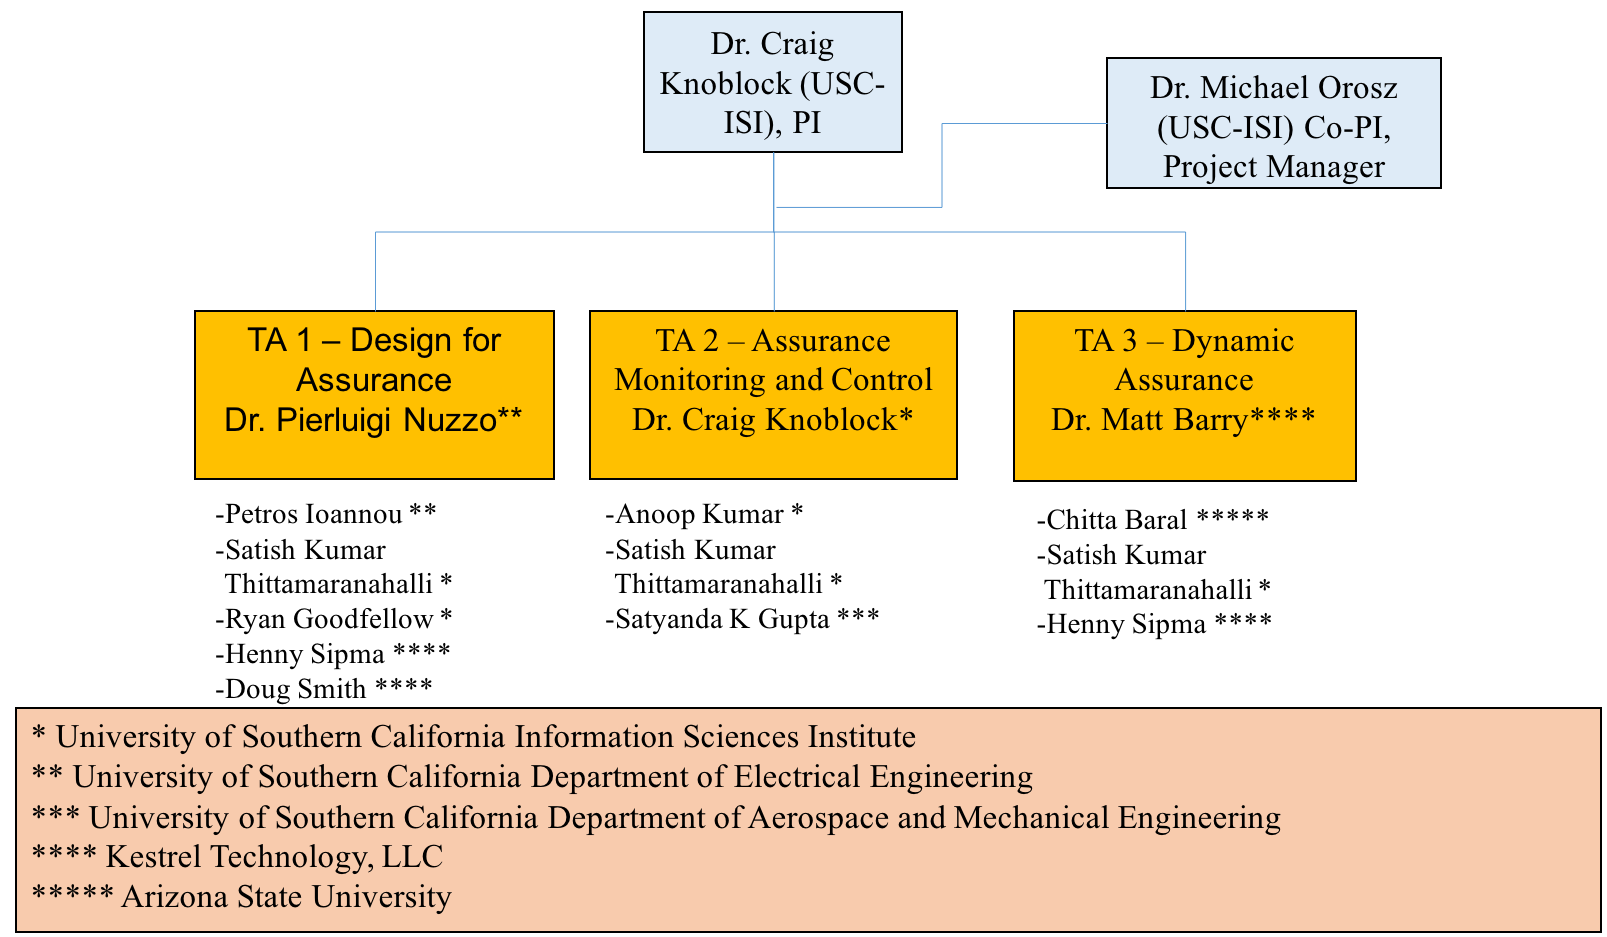
\includegraphics[width=6.0in]{./org-chart2.png}
\caption{\small Organization Chart}
\label{fig:org_chart}
\end{figure}

Coordination: To maximize collaboration and reduce risk to project failure from lack of communication and technical exchange, we plan to employ a wide variety of working styles and communication/coordination so that all can contribute.  At the core of our project will be regularly scheduled meetings bridging the diversely distributed team (Table~\ref{fig:Collaboration_Table}).  These meetings will address project status, identify challenges, implement risk mitigation strategies and participate in technology exchanges and system integration efforts (when appropriate)

\begin{table}[ht]
\caption{\small Project Meetings and Events}
  \centering
  {\footnotesize
\begin{tabular}{|m{3.15in}|m{3in}|} 
\hline
\textbf{Meeting} & \textbf{Frequency} 
\\\hline
Conference calls among investigators (discuss project status, address concerns and project risks) & Weekly
\\
\hline
Technical exchange and coordination meetings using Bluejeans or another videoconference technology & At least twice a month and more frequently as needed
  \\ 
\hline
Face-to-Face meetings (prior to P/I and demonstration meetings) & Every 3 to 6 months and more frequently (especially at the beginning of the project) as needed
 \\\cline{1-2}

\hline
\end{tabular}
}
\label{fig:Collaboration_Table}
\end{table}

\begin{table}[tbhp]
\caption{\small Key Project Team Member Responsibilities}
  \centering
  {\footnotesize
\begin{tabular}{| m{.75in} | m{3.9in}| m{1.5in}|} 
\hline
\textbf{Key Member} & \textbf{Responsibilities} & \textbf{Tasks} 
\\\hline
Dr.\ Craig Knoblock  & Principal Investigator responsible for project, leads TA 2 – Assurance Monitoring and Control.  Will lead the overall project and lead the TA2 team.  Served as the PI on many DARPA projects and has sucessfully led many large teams.    Effort on project:  25\% &
1.1.6, 1.2.2 1.2.3, 1.2.4, 1.3.4, 1.4.1, 
2.1.6, 2.2.2 2.2.3, 2.2.4, 2.3.4, 2.4.1, 
3.1.6, 3.2.2, 3.2.3, 3.2.4, 3.3.4, 3.4.1
\\
\hline
Dr.\ Michael Orosz & Co-Principal Investigator responsible managing the day-to-day operations of the project, assist technical teams as needed, coordinate with TA4 teams.    Has led many large complex multi-disciplined/multi-organizational projects in academic and industry environments.  Effort on project: 50\%
& 1.1.6, 2.1.6, 3.1.6, 1.4.1, 2.4.1, 3.4.1
  \\ 
\hline
Dr.\ Pierluigi Nuzzo 
& 
Co-Principal Investigator.  Leads the TA 1 - Design for Assurance team and conducts research on the formal methods for the design of the TA1 system.  Research experience on methodologies and tools for the design of cyber-physical systems; contracts, interfaces, and compositional methods for embedded system design; the application of automated formal methods and optimization theory to problems in embedded and cyber-physical systems.  Effort on project: 2 months/year (16.6\%)
& 
1.1.1, 2.1.1, 3.1.1 \\
\hline
Dr.\ Matthew Barry
& 
Key personnel.  Leads the TA 3 – Dynamic Assurance.   He will conduct the research on the dynamic assurance case language editors and parsers, the run-time system, and system integrations. Effort on project:  66\%
& 
1.3.2, 2.3.2, 3.3.2\\
\hline
Dr.\ Chitta Baral
& 
Key personnel responsible for learning assurance rules, supporting assurance rules with uncertainty and improving solver speed.  Expertise on ASP solvers, which will be used to reason about the assurance cases. Effort on project: 20\%
& 
1.3.1, 2.3.1, 3.3.1 \\
\hline
Dr.\ Doug Smith 
& 
Key personnel will support formal methods aspects of TA1, and lead the effort on abstract refinement. Expertise in field of automated correct-by-construction program generation.    Effort on project: 40\%
& 
1.1.5, 2.1.5, 3.1.5 \\
\hline
Dr.\ Henny Sipma
& 
Key personnel who will support the program verification tasks under TA1.  Will lead the effort on program verification.   Effort on project:  45\%
& 
1.1.5, 2.1.5, 3.1.5, 1.3.2, 2.3.2, 3.3.2 \\
\hline
Dr.\ Petros Ioannou
& 
Key personnel responsible providing and extending the assurance test bed, which will be available at the start of the project for autonomous vehicles.   Effort on project: 1 month/year (8.3\%)
& 
1.1.2, 2.1.2 (optional), 3.1.2 (optional)
\\
\hline
Dr.\ Satyandra Kumar Gupta
& 
Key Personnel providing autonomous command and control expertise to the TA-2 team.   Will lead the research on safety aware learning on TA2.   Past research on physics-aware decision making to facilitate automation.  Effort on project: 1 month/year (8.3\%)
& 
1.2.1, 2.2.1, 3.2.1 \\
\hline
Dr.\ Anoop Kumar 
& 
Key personnel providing support to the TA 2 project team.  Will lead the research on monitoring \& control and detecting distribution shifts.  Effort on project: 50\%
& 
1.2.1, 1.2.2, 1.2.3, 1.2.4, 2.2.1, 2.2.2, 2.2.3, 2.2.4, 3.2.1, 3.2.2, 3.2.3, 3.2.4\\
\hline
Dr.\ Satish Thittamaranahalli
& 
Key personnel developing scalable algorithms for TA1, TA2, and TA3 project teams.  Has extensive experience on scalable algorithm design, machine learning, and constraint reasoning.  Effort on project: 50\%
& 
1.2.1, 1.2.2, 1.2.3, 1.2.4, 2.2.1, 2.2.2, 2.2.3, 2.2.4, 3.2.1, 3.2.2, 3.2.3, 3.2.4, 1.1.4, 2.1.4, 3.1.4 \\
\hline
Dr.\ Ryan Goodfellow
& 
Key personnel providing support to the TA-1 project. Will lead the research on simulation-based testing.  Has extensive experience on simulation-based testing.  Effort on project:  30\%
& 
1.1.3, 2.1.3, 3.1.3 \\

\cline{1-2}

\hline
\end{tabular}
}
\label{fig:Table_Mgmt}
\end{table}



\newpage
\section{Personnel, Qualifications and Commitment}

{\bf Dr.\ Craig Knoblock}, the PI on this effort, is a Research Professor of both Computer Science and Spatial Sciences at the University of Southern California (USC) and Director of the Intelligent Systems Division at the USC Information Sciences Institute.   He received his Ph.D. from Carnegie Mellon University in computer science. 
%His research focuses on techniques for describing, acquiring, and exploiting the semantics of data.  
In previous projects he has worked on developing  scalable approaches to execution monitoring, accurate detection of sensor failures, and   automatic modeling and reconstruction of sensors.  He has published more than 300 journal articles, book chapters, and conference papers on these topics.  Dr. Knoblock is a Fellow of the Association for the Advancement of Artificial Intelligence (AAAI), a Distinguished Scientist of the Association of Computing Machinery (ACM), a Senior Member of IEEE, past President and Trustee of the International Joint Conference on Artificial Intelligence.
%and winner of the 2014 Robert S. Engelmore Award.  

{\bf Dr.\ Michael Orosz}, a Co-PI on this effort, is a Research Associate Professor of Civil and Environmental Engineering at the University of Southern California (USC) and Research Director of the Decision Systems Group at the USC Information Sciences Institute.  Dr. Orosz has over 30 years’ experience in commercial and government software development, basic and applied research, project management, academic research and has developed and deployed several commercially successful products.  His research interests are in machine learning and decision analytics as applied to intelligence analysis and autonomous command and control such as smart building controls.    Dr. Orosz has extensive experience in managing large complex multi-disciplined/multi-teamed research projects. %funded by DARPA, DHS, DoD, DoE, Industry, NASA, NRO, NSA and ONR.   
He received his Ph.D. in computer science from the University of California, Los Angeles.

{\bf Dr.\ Pierluigi Nuzzo}, a Co-PI on this project, is an Assistant Professor in the Department of Electrical Engineering at the University of Southern California. He received the Ph.D. in Electrical Engineering and Computer Sciences from the University of California at Berkeley. 
%in 2015, and the Laurea degree (MS) in electrical engineering (summa cum laude) from the University of Pisa, Italy, and the Sant'Anna School of Advanced Studies, Pisa, Italy.
%
%He has four years of research experience in analog and mixed signal circuit design as a researcher at IMEC, Leuven, Belgium, and over 10 years experience in design methodologies and tools for mixed-signal integrated circuits and cyber-physical systems, as a researcher at the University of Pisa, IMEC, UC Berkeley, and USC. 
His research interests
include: methodologies and tools for cyber-physical system and mixed-signal
system design; contracts, interfaces and compositional methods for embedded
system design; the application of formal methods and optimization theory to problems in embedded and cyber-physical systems and electronic design automation. 
%
Prof. Nuzzo received %First Place in the operational category and Best Overall
%Submission in the 2006 DAC/ISSCC Design Competition, 
a Marie Curie Fellowship
from the European Union in 2006, 
the University of California at Berkeley EECS
departmental fellowship in 2008, 
%the University of California at Berkeley Outstanding Graduate Student Instructor Award in 2013, 
the IBM Ph.D.
Fellowship in 2012 and 2014, 
%the Best Paper Award from the International Conference on Cyber-Physical Systems (ICCPS) in 2016, 
and the David J.~Sakrison Memorial Prize in 2016 for his doctoral research. 
%He is an author of 1 patent and over 60 publications.

{\bf Dr.\ Satyandra K. Gupta} is Smith International Professor in the Department of Aerospace and Mechanical Engineering at the University of Southern California. %Prior to joining the University of Southern California, he was a Professor in the Department of Mechanical Engineering and the Institute for Systems Research at the University of Maryland. He was the founding director of the Maryland Robotics Center and the Advanced Manufacturing Laboratory at the University of Maryland. 
He served as a program director for the National Robotics Initiative at the National Science Foundation from September 2012 to September 2014.  Dr. Gupta's interest is in the area of physics-aware decision making to facilitate automation. He has published more than 300 technical articles. He is a fellow of the American Society of Mechanical Engineers (ASME) and editor of ASME Journal of Computing and Information Science in Engineering. Dr. Gupta has received the Young Investigator Award from the Office of Naval Research in 2000, CAREER Award from the National Science Foundation in 2001, Presidential Early Career Award for Scientists and Engineers (PECASE) in 2001, Invention of the Year Award at the University of Maryland in 2007, Kos Ishii-Toshiba Award from ASME in 2011, and Excellence in Research Award from ASME in 2013.%, and Distinguished Alumnus Award from Indian Institute of Technology, Roorkee in 2014. %He has also received seven best paper awards at conferences.

{\bf Ryan Goodfellow} is a computer scientist at ISI working in combined cyber physical simulation and emulation platform development. His formal background is in simulation algorithms and modeling techniques using differential-algebraic equations (DAE). He has applied this knowledge in the CPS space by integrating DAE modeling languages and simulation engines with network testbeds to create comprehensive scientific experimentation platforms for cyber-physical systems. These experimentation platforms have been used in the power grid research space. %Ryan is a lead developer on the Deter network testbed, with a strong background in networked and distributed systems engineering. %He is also a combat veteran, serving as a non-commissioned officer and SIGINT team lead for a multi-functional intelligence team in Afghanistan.

{\bf Dr.\ Petros Ioannou} is a Professor in the Department of Electrical Engineering, Director of the Center for Advanced Transportation Technologies and Associate Director for Research for the DOT supported University Transportation Center at USC. He received his MS and PhD from the University of Illinois at Urbana Champaign in Mechanical and Electrical Engineering, respectively. His research interests are in robust adaptive control, vehicle dynamics and control, human factors and safety, automated vehicles, nonlinear systems and Intelligent transportation Systems.  He received the 2016 IEEE Transportation Technologies field award and the 2016 IEEE Control system society Transition to Practice Award. He is a Fellow of IEEE, IFAC and IET and author/coauthor of 8 books and over 400 papers.

{\bf Dr.\ Matthew Barry} will serve as lead for the TA3 tasks. %He will implement the dynamic assurance case language editors and parsers, the run-time system, and system integrations.  He will implement the assurance case arguments and the API for updating argument structure and content.  
Dr. Barry currently is CEO at Kestrel Technology LLC, and previously spent 20 years in NASA space mission operations at the Jet Propulsion Lab and Johnson Space Center.  At NASA Headquarters he led the introduction of dependability case requirements and plans for flight computing systems in upcoming manned space exploration missions, as well as the development of Agency-level software-related safety-critical control system requirements.  He recently served as a Principal Investigator on DHS/Cyber S\&T STAMP (Static Tool Analysis Modernization Program), DARPA CSFV (Crowd Sourced Formal Verification), three NASA Aeronautics R\&D projects, and the AFRL-sponsored Static Analysis of Numerical Algorithms project.  Dr. Barry earned BSME, MS, and PhD degrees in mechanical engineering, and an MBA degree, from Rice University.  

{\bf Dr.\ Henny Sipma} will support the program verification tasks under TA1.  %She is the key person behind the company's {\em KT Advance\/} and {\em KT Transferal\/} static analysis products, and the designer and programmer of the company's core {\em CodeHawk\/} abstract interpretation engine. 
Dr. Sipma currently is the CTO at Kestrel Technology LLC.  She has spent the past 10 years with Kestrel Technology as a static analysis expert; previously developed and taught static analysis techniques as senior research associate at Stanford University for eight years; and developed industrial process controls as an senior systems analyst at Shell.  She has been Principal Investigator or company lead on several recent R\&D projects for Federal agencies, including two projects under the IARPA STONESOUP (Securely Taking On New Executable Software of Uncertain Provenance) program; the DHS Cyber S\&T Gold Standard project; and the DARPA-sponsored STAC (Space-Time Analysis for Cybersecurity) and MUSE (Mining and Understanding Software Enclaves) programs.  Dr. Sipma earned 
%a BS degree in chemistry and an MS degree in chemical engineering at the University of Groningen in The Netherlands, and 
MS and PhD degrees in computer science from Stanford University.  

{\bf Dr.\ Douglas R.\ Smith} will support formal methods aspects of TA1, including the enforcement of safety properties and the generation of monitors.  He is President of Kestrel Technology LLC and Principal Scientist at Kestrel Institute.  He is a Fellow of the American Association of Artificial Intelligence (AAAI) and an ASE Fellow (Automated Software Engineering).  From 1986 to 2000, he taught an advanced graduate course on correct-by-construction software development at Stanford.  
%Dr. Smith has led the development of a series of software synthesis systems, including KIDS (Kestrel Interactive Development System), Specware, Designware, and Planware. 
%Applications domains have included a variety of complex high-performance planners and schedulers for the US Air Force.  He leads current projects on the generation of air mission plans and cyberoperations.  
Other recent projects focused on automated policy enforcement \cite{SmithD0703,SmithD08}, synthesis of secure network protocol codes, and the synthesis of high-performance constraint-solvers\cite{SmithD08c,SmithD13}.  Dr. Smith has over 30 years experience in the field of automated correct-by-construction program generation and has published over 100 papers. He has one patent.  He received the Ph.D. in Computer Science from Duke University% in 1979.  

{\bf Dr. Chitta Baral} is a Professor in the Department of Computer Science and Engineering at Arizona State University. He will support the TA3 efforts on Learning assurance rules, supporting assurance rules with uncertainty and improving solver speed. Dr. Baral has expertise in various aspects of autonomy and Artificial Intelligence. 
He wrote the first book on answer set programming (published by Cambridge University Press) the formal language behind our assurance rules. Some of his other works relevant to this proposal are: goal specification for autonomous systems, automatic construction of control rules for autonomous systems that satisfy given goals, combining machine learning with reasoning in various contexts, including image understanding. %He is the President of KR Inc. He is an associate editor of AIJ and has been an associate editor of JAIR.

{\bf Dr.\ Satish Kumar Thittamaranahalli (T. K. Satish Kumar)} leads the Collaboratory for Algorithmic Techniques and Artificial Intelligence (CATAI) at USC's Information Sciences Institute. He has published over 60 papers on numerous topics in Artificial Intelligence spanning such diverse areas as Constraint Reasoning, Planning and Scheduling, Probabilistic Reasoning, Robotics, Combinatorial Optimization, Approximation and Randomization, Heuristic Search, Model-Based Reasoning, Knowledge Representation and Spatio-Temporal Reasoning. %He %has served on the Program Committees of many international conferences in Artificial Intelligence
He and is a winner of the 2016 Best Robotics Paper Award and the 2005 Best Student Paper Award from the International Conference on Automated Planning and Scheduling. 
Dr. Kumar received his PhD in Computer Science from Stanford University. %In the past, he has also been a Visiting Student at the NASA Ames Research Center, a Postdoctoral Research Scholar at the University of California, Berkeley, a Research Scientist at the Institute for Human and Machine Cognition, a Visiting Assistant Professor at the University of West Florida, and a Senior Research and Development Scientist at Mission Critical Technologies.

\textbf{Dr.\ Anoop Kumar} is a senior computer scientist at USC ISI and has broad expertise in machine learning, statistical modeling, and software engineering.  Dr.\ Kumar is the technical lead on the DARPA RSPACE program and has played a vital role in developing a system that fuses air operations data from multiple sources, maintains world state, and issues warnings. Previously, he led the research and development of the BBN’s election forecasting system for the IARPA OSI program. %Dr.\ Kumar played a significant role in the DARPA DEFT program by developing a model to support integration of output from multiple NLP algorithms. He has contributed at the development to management levels on government research contracts and commercial projects. 
Dr.\ Kumar helped design and develop BBN's commercially available, hosted speech and medical transcription services offering. 

\begin{table}[!tbh]
\begin{footnotesize}
\vspace{-0.1in}

\begin{tabular}{lll}
\begin{tabular}[t]{|l|@{}c@{}|@{}c@{}|@{}c@{}|@{}c@{}|} \hline
Project & Status & \multicolumn{3}{ c| }{Hours} \\ \cline{3-5}
& & P1 & P2 & P3 \\ \hline



\multicolumn{5}{ |c| }{ \textbf{Craig Knoblock} } \\ \cline{1-5}
Safeguard & Pro & 770 & 641 & 641 \\ \cline{1-5}
ELICIT & Cur & 308 & 256 & 120 \\ \cline{1-5}
WTNIC & Cur & 11 & 0 & 0 \\ \cline{1-5}
EFFECT & Cur & 641 & 107 & 0 \\ \cline{1-5}
LinkedMaps & Cur & 203 & 25 & 0 \\ \cline{1-5}
PRINCESS & Cur & 608 & 96 & 0 \\ \cline{1-5}
SCHARP & Cur & 481 & 54 & 0 \\ \cline{1-5}
MINT & Pen & 650 & 534 & 285 \\ \cline{1-5}

\multicolumn{5}{ |c| }{ \textbf{Michael Orosz} } \\ \cline{1-5}
Safeguard & Pro & 1560 & 1300 & 1300  \\ \cline{1-5}
SMC/SY & Cur & 1803 & 0 & 0  \\ \cline{1-5}

\multicolumn{5}{ |c| }{ \textbf{Matthew Barry} } \\ \cline{1-5}
Safeguard & Pro & 2078 & 1690 & 1554 \\ \cline{1-5}
Starlite & Cur & 1840 & 1692 & 0 \\ \cline{1-5}



\multicolumn{5}{ |c| }{ \textbf{Anoop Kumar} } \\ \cline{1-5}
Safeguard & Pro & 1560 & 1300 & 1300 \\ \cline{1-5}

\end{tabular}
&
\begin{tabular}[t]{|l|@{}c@{}|@{}c@{}|@{}c@{}|@{}c@{}|} \hline
Project & Status & \multicolumn{3}{ c| }{Hours} \\ \cline{3-5}
& & P1 & P2 & P3 \\ \hline

\multicolumn{5}{ |c| }{ \textbf{Pierluigi Nuzzo} } \\ \cline{1-5}
Safeguard & Pro & 520 & 433 & 433  \\ \cline{1-5}
Mirage & Cur & 433 & 0 & 0  \\ \cline{1-5}

\multicolumn{5}{ |c| }{ \textbf{Satyandra Gupta} } \\ \cline{1-5}
Safeguard & Pro & 260 & 217 & 217 \\ \cline{1-5}
Human   & Cur & 22 & 0 & 0 \\ \cline{1-5}
Vehicles & Cur & 36 & 0 & 0 \\ \cline{1-5}
Robot & Cur & 116 & 0 & 0 \\ \cline{1-5}
Assembly & Cur & 33 & 0 & 0 \\ \cline{1-5}
Solar & Cur & 4 & 0 & 0 \\ \cline{1-5}

\multicolumn{5}{ |c| }{ \textbf{Petros Ioannou} } \\ \cline{1-5}
Safeguard & Pro & 260 & 217 & 217 \\ \cline{1-5}
CPS & Cur & 130 & 0 & 0 \\ \cline{1-5}

\multicolumn{5}{ |c| }{ \textbf{Ryan Goodfellow} } \\ \cline{1-5}
Safeguard & Pro & 936 & 780 & 780 \\ \cline{1-5}
STEAM & Cur & 416 & 0 & 0 \\ \cline{1-5}


\end{tabular}
&
\begin{tabular}[t]{|l|@{}c@{}|@{}c@{}|@{}c@{}|@{}c@{}|} \hline
Project & Status & \multicolumn{3}{ c| }{Hours} \\ \cline{3-5}
& & P1 & P2 & P3 \\ \hline

\multicolumn{5}{ |c| }{ \textbf{Chitta Baral} } \\ \cline{1-5}
Safeguard & Pro & 659 & 485 & 485 \\ \cline{1-5}
PostdocBP & Cur & 176 & 0 & 0 \\ \cline{1-5}
Languages & Pen & 528 & 264 & 264 \\ \cline{1-5}
CAREER & Pen & 88 & 44 & 44 \\ \cline{1-5}
CHS & Pen & 510 & 255 & 0 \\ \cline{1-5}

\multicolumn{5}{ |c| }{ \textbf{Doug Smith} } \\ \cline{1-5}
Safeguard & Pro & 1222 & 984 & 840 \\ \cline{1-5}
RSPACE & Cur & 342 & 0 & 0 \\ 
\cline{1-5}
PLANX & Cur & 154 & 0 & 0 \\ 
\cline{1-5}
HACCS & Pen & 923 & 769 & 769 \\ 
\cline{1-5}

\multicolumn{5}{ |c| }{ \textbf{Henny Sipma} } \\ \cline{1-5}
Safeguard & Pro & 1372 & 962 & 840 \\ \cline{1-5}
STAC & Cur & 797 & 0 & 0 \\ \cline{1-5}

\multicolumn{5}{ |c| }{ \textbf{Satish Thittamaranahalli} } \\ \cline{1-5}
Safeguard & Pro & 1560 & 1300 & 1300 \\ \cline{1-5}
MapF & Cur & 103 & 103 & 0 \\ \cline{1-5}

\end{tabular}
\end{tabular}

\end{footnotesize}
\caption{Individual commitments of key personnel}
\label{tab:Commitments}
\vspace{-0.2in}
\end{table}

\clearpage
\newpage
\section{Capabilities}


%\subsection{University of Southern California}
USC has strengths in number of areas that are closely related to the proposed work:
\begin{itemize}[itemsep=0pt,leftmargin=*]
\item Dr.\ Nuzzo 
%has over 10-year research experience in embedded system design, from mixed-signal chip design (analog-to-digital converters, frequency synthesizers, software-defined radio), to methodologies and tools for mixed-signal integrated circuits and Cyber-Physical Systems (CPSs), and the application of formal methods and optimization theory to problems in embedded and cyber-physical systems and electronic design automation.  
%His doctoral work 
has done extensive research on contracts and compositional methods for heterogeneous system design and design space exploration, with application to aircraft electric power systems and environmental control systems. His work has helped transition rigorous system design foundations, innovative design methodologies, and new systems engineering paradigms to industry (IBM, United Technologies). 
\item Dr.\ Satyandra K. Gupta has worked on autonomous surface vehicles, autonomous ground vehicles for operation on rugged terrains, and autonomous flapping wing aerial vehicles.   His group has developed a hierarchal decision making approach for realizing autonomous systems. 
%This approach combines task planning and assignment, deliberative trajectory planning, reactive collision avoidance behaviors, and trajectory tracking control layers. 
His group has also developed new methods for learning reactive behaviors in adversarial environments and COLREGS compliant trajectory planning. \item Dr.\ Knoblock has developed methods that learn the relationships between sensors to both identify failures and changes in sensor and reconstruct those sensors, providing estimates of the accuracy of the reconstructed sensors.  
\item Ryan Goodfellow has extensive experience in simulation based testing through high-fidelity CPS testbed environment development and operation, using the Deter network testbed as the core which has supported several large scale government projects from a variety of agencies and thousands of users. %we have developed sophisticated CPS experiments under programs such as NFS RIPS, NIST SmartCities and the DHS Cybersecurity showcase.
\item Dr.\ Ioannou %helped  design and implement adaptive cruise control systems in collaboration with Ford Motor Company, which was commercialized four years before any other company. He 
worked on several DOT funded projects on automated vehicles and intelligent highway systems where he demonstrated his vehicle control designs for safety and performance on actual automated vehicles in test trucks and I-15 highway.
\item Drs.\ Knoblock, Kumar, and Thittamaranahalli have developed highly scalable approaches for monitoring message traffic to identify potential problems and issue warnings and alerts. 
\item Dr. Thittamaranahalli has developed state-of-the-art methods for efficiently solving large-scale search and optimization problems. %These techniques will be applicable in TA2 for safety-aware learning and planning, in TA2 for assurance monitoring and control, and in TA3 for dynamic assessment of assurance cases.

\end{itemize}
%\subsection{Kestrel Technology LLC}

Kestrel Technology's strength is in program analysis, specifically static analysis of both source and binary targets.  The company performs applied R\&D and product development for a variety of static analysis applications  pivoting primarily on the abstract interpretation technique.  The company recently initiated development of program analysis applications using logical equivalence techniques. As a provider of verification evidence in the form of mathematical proofs, the company also has expertise in the design and development of assurance case arguments for high-integrity systems using such evidence. %The company is engaged in a partnership with Wind River Systems to develop program analysis tools for its embedded system developers.  Many of Wind River's customers must develop their products under safety and certification standards, including those using safety cases.  

   

%\subsection{Arizona State University}
Chitta Baral at Arizona State University has developed various software to learn assurance rules and various ASP solvers, which he has made available as open-source.

Most of the software carried forward for implementation or derivation is open source.  The single exception is Kestrel Technology's {\it KT Advance\/} static analysis tool (TA1), in particular the abstract interpretation engine therein, which is company proprietary and is US EAR export-controlled.   
%Owing to mixed funding for the development of that technology 
We will continue to provide the Federal government a restricted use license for that particular item.

There are no specialized facilities, data, or GFE required for this effort. 

\include{sow}
\include{milestones}

% \section{Level of Effort by Task \textcolor{red}{[Mike/Lisa - 1 pages]}}

% \textcolor{blue}{
% \begin{itemize}
% \item Will be a separate spreadsheet
% \item
% \end{itemize}
% }

\include{appendix_a}

%\section{Appendix B \textcolor{red}{[No Page Count]}}

\section{References}
\bibliographystyle{acm} 
\bibliography{TA3/ta3,TA2/ta2,TA1/ta1}
\end{document}
\clearpage
\newpage


\section{Management Plan}


The Principal Investigator for this effort is Dr. Craig Knoblock who is responsible for all aspects of the effort, will coordinate the parallel team efforts, and will ensure high levels of performance from individual team members.  The Co-P/I, Dr. Michael Orosz, will provide project management and will assist all performers in the execution of the project.    The project team is divided into three working groups (Figure~\ref{fig:org_chart}) corresponding to Technical Areas 1-3, however, members of each team contribute across all project activities.   Table~\ref{fig:Table_Mgmt} defines the major contributions of each project team member to the project tasks.

\begin{figure}[tbhp]
%\vspace{-25pt}
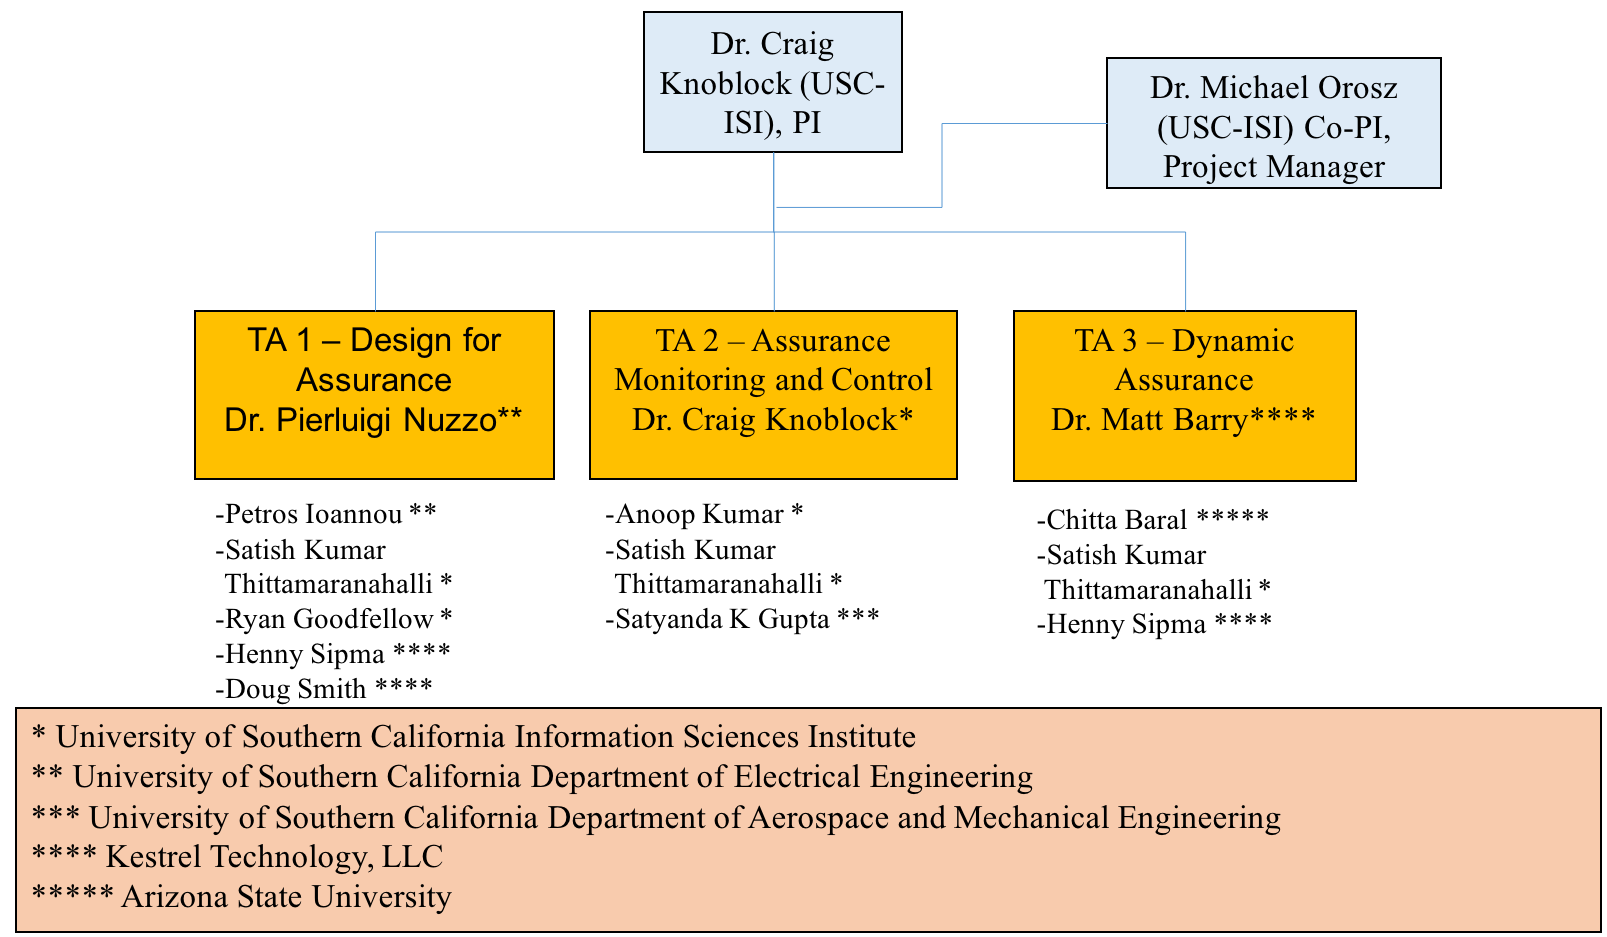
\includegraphics[width=6.0in]{./org-chart2.png}
\caption{\small Organization Chart}
\label{fig:org_chart}
\end{figure}

Coordination: To maximize collaboration and reduce risk to project failure from lack of communication and technical exchange, we plan to employ a wide variety of working styles and communication/coordination so that all can contribute.  At the core of our project will be regularly scheduled meetings bridging the diversely distributed team (Table~\ref{fig:Collaboration_Table}).  These meetings will address project status, identify challenges, implement risk mitigation strategies and participate in technology exchanges and system integration efforts (when appropriate)

\begin{table}[ht]
\caption{\small Project Meetings and Events}
  \centering
  {\footnotesize
\begin{tabular}{|m{3.15in}|m{3in}|} 
\hline
\textbf{Meeting} & \textbf{Frequency} 
\\\hline
Conference calls among investigators (discuss project status, address concerns and project risks) & Weekly
\\
\hline
Technical exchange and coordination meetings using Bluejeans or another videoconference technology & At least twice a month and more frequently as needed
  \\ 
\hline
Face-to-Face meetings (prior to P/I and demonstration meetings) & Every 3 to 6 months and more frequently (especially at the beginning of the project) as needed
 \\\cline{1-2}

\hline
\end{tabular}
}
\label{fig:Collaboration_Table}
\end{table}

\begin{table}[tbhp]
\caption{\small Key Project Team Member Responsibilities}
  \centering
  {\footnotesize
\begin{tabular}{| m{.75in} | m{3.9in}| m{1.5in}|} 
\hline
\textbf{Key Member} & \textbf{Responsibilities} & \textbf{Tasks} 
\\\hline
Dr.\ Craig Knoblock  & Principal Investigator responsible for project, leads TA 2 – Assurance Monitoring and Control.  Will lead the overall project and lead the TA2 team.  Served as the PI on many DARPA projects and has sucessfully led many large teams.    Effort on project:  25\% &
1.1.6, 1.2.2 1.2.3, 1.2.4, 1.3.4, 1.4.1, 
2.1.6, 2.2.2 2.2.3, 2.2.4, 2.3.4, 2.4.1, 
3.1.6, 3.2.2, 3.2.3, 3.2.4, 3.3.4, 3.4.1
\\
\hline
Dr.\ Michael Orosz & Co-Principal Investigator responsible managing the day-to-day operations of the project, assist technical teams as needed, coordinate with TA4 teams.    Has led many large complex multi-disciplined/multi-organizational projects in academic and industry environments.  Effort on project: 50\%
& 1.1.6, 2.1.6, 3.1.6, 1.4.1, 2.4.1, 3.4.1
  \\ 
\hline
Dr.\ Pierluigi Nuzzo 
& 
Co-Principal Investigator.  Leads the TA 1 - Design for Assurance team and conducts research on the formal methods for the design of the TA1 system.  Research experience on methodologies and tools for the design of cyber-physical systems; contracts, interfaces, and compositional methods for embedded system design; the application of automated formal methods and optimization theory to problems in embedded and cyber-physical systems.  Effort on project: 2 months/year (16.6\%)
& 
1.1.1, 2.1.1, 3.1.1 \\
\hline
Dr.\ Matthew Barry
& 
Key personnel.  Leads the TA 3 – Dynamic Assurance.   He will conduct the research on the dynamic assurance case language editors and parsers, the run-time system, and system integrations. Effort on project:  66\%
& 
1.3.2, 2.3.2, 3.3.2\\
\hline
Dr.\ Chitta Baral
& 
Key personnel responsible for learning assurance rules, supporting assurance rules with uncertainty and improving solver speed.  Expertise on ASP solvers, which will be used to reason about the assurance cases. Effort on project: 20\%
& 
1.3.1, 2.3.1, 3.3.1 \\
\hline
Dr.\ Doug Smith 
& 
Key personnel will support formal methods aspects of TA1, and lead the effort on abstract refinement. Expertise in field of automated correct-by-construction program generation.    Effort on project: 40\%
& 
1.1.5, 2.1.5, 3.1.5 \\
\hline
Dr.\ Henny Sipma
& 
Key personnel who will support the program verification tasks under TA1.  Will lead the effort on program verification.   Effort on project:  45\%
& 
1.1.5, 2.1.5, 3.1.5, 1.3.2, 2.3.2, 3.3.2 \\
\hline
Dr.\ Petros Ioannou
& 
Key personnel responsible providing and extending the assurance test bed, which will be available at the start of the project for autonomous vehicles.   Effort on project: 1 month/year (8.3\%)
& 
1.1.2, 2.1.2 (optional), 3.1.2 (optional)
\\
\hline
Dr.\ Satyandra Kumar Gupta
& 
Key Personnel providing autonomous command and control expertise to the TA-2 team.   Will lead the research on safety aware learning on TA2.   Past research on physics-aware decision making to facilitate automation.  Effort on project: 1 month/year (8.3\%)
& 
1.2.1, 2.2.1, 3.2.1 \\
\hline
Dr.\ Anoop Kumar 
& 
Key personnel providing support to the TA 2 project team.  Will lead the research on monitoring \& control and detecting distribution shifts.  Effort on project: 50\%
& 
1.2.1, 1.2.2, 1.2.3, 1.2.4, 2.2.1, 2.2.2, 2.2.3, 2.2.4, 3.2.1, 3.2.2, 3.2.3, 3.2.4\\
\hline
Dr.\ Satish Thittamaranahalli
& 
Key personnel developing scalable algorithms for TA1, TA2, and TA3 project teams.  Has extensive experience on scalable algorithm design, machine learning, and constraint reasoning.  Effort on project: 50\%
& 
1.2.1, 1.2.2, 1.2.3, 1.2.4, 2.2.1, 2.2.2, 2.2.3, 2.2.4, 3.2.1, 3.2.2, 3.2.3, 3.2.4, 1.1.4, 2.1.4, 3.1.4 \\
\hline
Dr.\ Ryan Goodfellow
& 
Key personnel providing support to the TA-1 project. Will lead the research on simulation-based testing.  Has extensive experience on simulation-based testing.  Effort on project:  30\%
& 
1.1.3, 2.1.3, 3.1.3 \\

\cline{1-2}

\hline
\end{tabular}
}
\label{fig:Table_Mgmt}
\end{table}



\newpage
\section{Personnel, Qualifications and Commitment}

{\bf Dr.\ Craig Knoblock}, the PI on this effort, is a Research Professor of both Computer Science and Spatial Sciences at the University of Southern California (USC) and Director of the Intelligent Systems Division at the USC Information Sciences Institute.   He received his Ph.D. from Carnegie Mellon University in computer science. 
%His research focuses on techniques for describing, acquiring, and exploiting the semantics of data.  
In previous projects he has worked on developing  scalable approaches to execution monitoring, accurate detection of sensor failures, and   automatic modeling and reconstruction of sensors.  He has published more than 300 journal articles, book chapters, and conference papers on these topics.  Dr. Knoblock is a Fellow of the Association for the Advancement of Artificial Intelligence (AAAI), a Distinguished Scientist of the Association of Computing Machinery (ACM), a Senior Member of IEEE, past President and Trustee of the International Joint Conference on Artificial Intelligence.
%and winner of the 2014 Robert S. Engelmore Award.  

{\bf Dr.\ Michael Orosz}, a Co-PI on this effort, is a Research Associate Professor of Civil and Environmental Engineering at the University of Southern California (USC) and Research Director of the Decision Systems Group at the USC Information Sciences Institute.  Dr. Orosz has over 30 years’ experience in commercial and government software development, basic and applied research, project management, academic research and has developed and deployed several commercially successful products.  His research interests are in machine learning and decision analytics as applied to intelligence analysis and autonomous command and control such as smart building controls.    Dr. Orosz has extensive experience in managing large complex multi-disciplined/multi-teamed research projects. %funded by DARPA, DHS, DoD, DoE, Industry, NASA, NRO, NSA and ONR.   
He received his Ph.D. in computer science from the University of California, Los Angeles.

{\bf Dr.\ Pierluigi Nuzzo}, a Co-PI on this project, is an Assistant Professor in the Department of Electrical Engineering at the University of Southern California. He received the Ph.D. in Electrical Engineering and Computer Sciences from the University of California at Berkeley. 
%in 2015, and the Laurea degree (MS) in electrical engineering (summa cum laude) from the University of Pisa, Italy, and the Sant'Anna School of Advanced Studies, Pisa, Italy.
%
%He has four years of research experience in analog and mixed signal circuit design as a researcher at IMEC, Leuven, Belgium, and over 10 years experience in design methodologies and tools for mixed-signal integrated circuits and cyber-physical systems, as a researcher at the University of Pisa, IMEC, UC Berkeley, and USC. 
His research interests
include: methodologies and tools for cyber-physical system and mixed-signal
system design; contracts, interfaces and compositional methods for embedded
system design; the application of formal methods and optimization theory to problems in embedded and cyber-physical systems and electronic design automation. 
%
Prof. Nuzzo received %First Place in the operational category and Best Overall
%Submission in the 2006 DAC/ISSCC Design Competition, 
a Marie Curie Fellowship
from the European Union in 2006, 
the University of California at Berkeley EECS
departmental fellowship in 2008, 
%the University of California at Berkeley Outstanding Graduate Student Instructor Award in 2013, 
the IBM Ph.D.
Fellowship in 2012 and 2014, 
%the Best Paper Award from the International Conference on Cyber-Physical Systems (ICCPS) in 2016, 
and the David J.~Sakrison Memorial Prize in 2016 for his doctoral research. 
%He is an author of 1 patent and over 60 publications.

{\bf Dr.\ Satyandra K. Gupta} is Smith International Professor in the Department of Aerospace and Mechanical Engineering at the University of Southern California. %Prior to joining the University of Southern California, he was a Professor in the Department of Mechanical Engineering and the Institute for Systems Research at the University of Maryland. He was the founding director of the Maryland Robotics Center and the Advanced Manufacturing Laboratory at the University of Maryland. 
He served as a program director for the National Robotics Initiative at the National Science Foundation from September 2012 to September 2014.  Dr. Gupta's interest is in the area of physics-aware decision making to facilitate automation. He has published more than 300 technical articles. He is a fellow of the American Society of Mechanical Engineers (ASME) and editor of ASME Journal of Computing and Information Science in Engineering. Dr. Gupta has received the Young Investigator Award from the Office of Naval Research in 2000, CAREER Award from the National Science Foundation in 2001, Presidential Early Career Award for Scientists and Engineers (PECASE) in 2001, Invention of the Year Award at the University of Maryland in 2007, Kos Ishii-Toshiba Award from ASME in 2011, and Excellence in Research Award from ASME in 2013.%, and Distinguished Alumnus Award from Indian Institute of Technology, Roorkee in 2014. %He has also received seven best paper awards at conferences.

{\bf Ryan Goodfellow} is a computer scientist at ISI working in combined cyber physical simulation and emulation platform development. His formal background is in simulation algorithms and modeling techniques using differential-algebraic equations (DAE). He has applied this knowledge in the CPS space by integrating DAE modeling languages and simulation engines with network testbeds to create comprehensive scientific experimentation platforms for cyber-physical systems. These experimentation platforms have been used in the power grid research space. %Ryan is a lead developer on the Deter network testbed, with a strong background in networked and distributed systems engineering. %He is also a combat veteran, serving as a non-commissioned officer and SIGINT team lead for a multi-functional intelligence team in Afghanistan.

{\bf Dr.\ Petros Ioannou} is a Professor in the Department of Electrical Engineering, Director of the Center for Advanced Transportation Technologies and Associate Director for Research for the DOT supported University Transportation Center at USC. He received his MS and PhD from the University of Illinois at Urbana Champaign in Mechanical and Electrical Engineering, respectively. His research interests are in robust adaptive control, vehicle dynamics and control, human factors and safety, automated vehicles, nonlinear systems and Intelligent transportation Systems.  He received the 2016 IEEE Transportation Technologies field award and the 2016 IEEE Control system society Transition to Practice Award. He is a Fellow of IEEE, IFAC and IET and author/coauthor of 8 books and over 400 papers.

{\bf Dr.\ Matthew Barry} will serve as lead for the TA3 tasks. %He will implement the dynamic assurance case language editors and parsers, the run-time system, and system integrations.  He will implement the assurance case arguments and the API for updating argument structure and content.  
Dr. Barry currently is CEO at Kestrel Technology LLC, and previously spent 20 years in NASA space mission operations at the Jet Propulsion Lab and Johnson Space Center.  At NASA Headquarters he led the introduction of dependability case requirements and plans for flight computing systems in upcoming manned space exploration missions, as well as the development of Agency-level software-related safety-critical control system requirements.  He recently served as a Principal Investigator on DHS/Cyber S\&T STAMP (Static Tool Analysis Modernization Program), DARPA CSFV (Crowd Sourced Formal Verification), three NASA Aeronautics R\&D projects, and the AFRL-sponsored Static Analysis of Numerical Algorithms project.  Dr. Barry earned BSME, MS, and PhD degrees in mechanical engineering, and an MBA degree, from Rice University.  

{\bf Dr.\ Henny Sipma} will support the program verification tasks under TA1.  %She is the key person behind the company's {\em KT Advance\/} and {\em KT Transferal\/} static analysis products, and the designer and programmer of the company's core {\em CodeHawk\/} abstract interpretation engine. 
Dr. Sipma currently is the CTO at Kestrel Technology LLC.  She has spent the past 10 years with Kestrel Technology as a static analysis expert; previously developed and taught static analysis techniques as senior research associate at Stanford University for eight years; and developed industrial process controls as an senior systems analyst at Shell.  She has been Principal Investigator or company lead on several recent R\&D projects for Federal agencies, including two projects under the IARPA STONESOUP (Securely Taking On New Executable Software of Uncertain Provenance) program; the DHS Cyber S\&T Gold Standard project; and the DARPA-sponsored STAC (Space-Time Analysis for Cybersecurity) and MUSE (Mining and Understanding Software Enclaves) programs.  Dr. Sipma earned 
%a BS degree in chemistry and an MS degree in chemical engineering at the University of Groningen in The Netherlands, and 
MS and PhD degrees in computer science from Stanford University.  

{\bf Dr.\ Douglas R.\ Smith} will support formal methods aspects of TA1, including the enforcement of safety properties and the generation of monitors.  He is President of Kestrel Technology LLC and Principal Scientist at Kestrel Institute.  He is a Fellow of the American Association of Artificial Intelligence (AAAI) and an ASE Fellow (Automated Software Engineering).  From 1986 to 2000, he taught an advanced graduate course on correct-by-construction software development at Stanford.  
%Dr. Smith has led the development of a series of software synthesis systems, including KIDS (Kestrel Interactive Development System), Specware, Designware, and Planware. 
%Applications domains have included a variety of complex high-performance planners and schedulers for the US Air Force.  He leads current projects on the generation of air mission plans and cyberoperations.  
Other recent projects focused on automated policy enforcement \cite{SmithD0703,SmithD08}, synthesis of secure network protocol codes, and the synthesis of high-performance constraint-solvers\cite{SmithD08c,SmithD13}.  Dr. Smith has over 30 years experience in the field of automated correct-by-construction program generation and has published over 100 papers. He has one patent.  He received the Ph.D. in Computer Science from Duke University% in 1979.  

{\bf Dr. Chitta Baral} is a Professor in the Department of Computer Science and Engineering at Arizona State University. He will support the TA3 efforts on Learning assurance rules, supporting assurance rules with uncertainty and improving solver speed. Dr. Baral has expertise in various aspects of autonomy and Artificial Intelligence. 
He wrote the first book on answer set programming (published by Cambridge University Press) the formal language behind our assurance rules. Some of his other works relevant to this proposal are: goal specification for autonomous systems, automatic construction of control rules for autonomous systems that satisfy given goals, combining machine learning with reasoning in various contexts, including image understanding. %He is the President of KR Inc. He is an associate editor of AIJ and has been an associate editor of JAIR.

{\bf Dr.\ Satish Kumar Thittamaranahalli (T. K. Satish Kumar)} leads the Collaboratory for Algorithmic Techniques and Artificial Intelligence (CATAI) at USC's Information Sciences Institute. He has published over 60 papers on numerous topics in Artificial Intelligence spanning such diverse areas as Constraint Reasoning, Planning and Scheduling, Probabilistic Reasoning, Robotics, Combinatorial Optimization, Approximation and Randomization, Heuristic Search, Model-Based Reasoning, Knowledge Representation and Spatio-Temporal Reasoning. %He %has served on the Program Committees of many international conferences in Artificial Intelligence
He and is a winner of the 2016 Best Robotics Paper Award and the 2005 Best Student Paper Award from the International Conference on Automated Planning and Scheduling. 
Dr. Kumar received his PhD in Computer Science from Stanford University. %In the past, he has also been a Visiting Student at the NASA Ames Research Center, a Postdoctoral Research Scholar at the University of California, Berkeley, a Research Scientist at the Institute for Human and Machine Cognition, a Visiting Assistant Professor at the University of West Florida, and a Senior Research and Development Scientist at Mission Critical Technologies.

\textbf{Dr.\ Anoop Kumar} is a senior computer scientist at USC ISI and has broad expertise in machine learning, statistical modeling, and software engineering.  Dr.\ Kumar is the technical lead on the DARPA RSPACE program and has played a vital role in developing a system that fuses air operations data from multiple sources, maintains world state, and issues warnings. Previously, he led the research and development of the BBN’s election forecasting system for the IARPA OSI program. %Dr.\ Kumar played a significant role in the DARPA DEFT program by developing a model to support integration of output from multiple NLP algorithms. He has contributed at the development to management levels on government research contracts and commercial projects. 
Dr.\ Kumar helped design and develop BBN's commercially available, hosted speech and medical transcription services offering. 

\begin{table}[!tbh]
\begin{footnotesize}
\vspace{-0.1in}

\begin{tabular}{lll}
\begin{tabular}[t]{|l|@{}c@{}|@{}c@{}|@{}c@{}|@{}c@{}|} \hline
Project & Status & \multicolumn{3}{ c| }{Hours} \\ \cline{3-5}
& & P1 & P2 & P3 \\ \hline



\multicolumn{5}{ |c| }{ \textbf{Craig Knoblock} } \\ \cline{1-5}
Safeguard & Pro & 770 & 641 & 641 \\ \cline{1-5}
ELICIT & Cur & 308 & 256 & 120 \\ \cline{1-5}
WTNIC & Cur & 11 & 0 & 0 \\ \cline{1-5}
EFFECT & Cur & 641 & 107 & 0 \\ \cline{1-5}
LinkedMaps & Cur & 203 & 25 & 0 \\ \cline{1-5}
PRINCESS & Cur & 608 & 96 & 0 \\ \cline{1-5}
SCHARP & Cur & 481 & 54 & 0 \\ \cline{1-5}
MINT & Pen & 650 & 534 & 285 \\ \cline{1-5}

\multicolumn{5}{ |c| }{ \textbf{Michael Orosz} } \\ \cline{1-5}
Safeguard & Pro & 1560 & 1300 & 1300  \\ \cline{1-5}
SMC/SY & Cur & 1803 & 0 & 0  \\ \cline{1-5}

\multicolumn{5}{ |c| }{ \textbf{Matthew Barry} } \\ \cline{1-5}
Safeguard & Pro & 2078 & 1690 & 1554 \\ \cline{1-5}
Starlite & Cur & 1840 & 1692 & 0 \\ \cline{1-5}



\multicolumn{5}{ |c| }{ \textbf{Anoop Kumar} } \\ \cline{1-5}
Safeguard & Pro & 1560 & 1300 & 1300 \\ \cline{1-5}

\end{tabular}
&
\begin{tabular}[t]{|l|@{}c@{}|@{}c@{}|@{}c@{}|@{}c@{}|} \hline
Project & Status & \multicolumn{3}{ c| }{Hours} \\ \cline{3-5}
& & P1 & P2 & P3 \\ \hline

\multicolumn{5}{ |c| }{ \textbf{Pierluigi Nuzzo} } \\ \cline{1-5}
Safeguard & Pro & 520 & 433 & 433  \\ \cline{1-5}
Mirage & Cur & 433 & 0 & 0  \\ \cline{1-5}

\multicolumn{5}{ |c| }{ \textbf{Satyandra Gupta} } \\ \cline{1-5}
Safeguard & Pro & 260 & 217 & 217 \\ \cline{1-5}
Human   & Cur & 22 & 0 & 0 \\ \cline{1-5}
Vehicles & Cur & 36 & 0 & 0 \\ \cline{1-5}
Robot & Cur & 116 & 0 & 0 \\ \cline{1-5}
Assembly & Cur & 33 & 0 & 0 \\ \cline{1-5}
Solar & Cur & 4 & 0 & 0 \\ \cline{1-5}

\multicolumn{5}{ |c| }{ \textbf{Petros Ioannou} } \\ \cline{1-5}
Safeguard & Pro & 260 & 217 & 217 \\ \cline{1-5}
CPS & Cur & 130 & 0 & 0 \\ \cline{1-5}

\multicolumn{5}{ |c| }{ \textbf{Ryan Goodfellow} } \\ \cline{1-5}
Safeguard & Pro & 936 & 780 & 780 \\ \cline{1-5}
STEAM & Cur & 416 & 0 & 0 \\ \cline{1-5}


\end{tabular}
&
\begin{tabular}[t]{|l|@{}c@{}|@{}c@{}|@{}c@{}|@{}c@{}|} \hline
Project & Status & \multicolumn{3}{ c| }{Hours} \\ \cline{3-5}
& & P1 & P2 & P3 \\ \hline

\multicolumn{5}{ |c| }{ \textbf{Chitta Baral} } \\ \cline{1-5}
Safeguard & Pro & 659 & 485 & 485 \\ \cline{1-5}
PostdocBP & Cur & 176 & 0 & 0 \\ \cline{1-5}
Languages & Pen & 528 & 264 & 264 \\ \cline{1-5}
CAREER & Pen & 88 & 44 & 44 \\ \cline{1-5}
CHS & Pen & 510 & 255 & 0 \\ \cline{1-5}

\multicolumn{5}{ |c| }{ \textbf{Doug Smith} } \\ \cline{1-5}
Safeguard & Pro & 1222 & 984 & 840 \\ \cline{1-5}
RSPACE & Cur & 342 & 0 & 0 \\ 
\cline{1-5}
PLANX & Cur & 154 & 0 & 0 \\ 
\cline{1-5}
HACCS & Pen & 923 & 769 & 769 \\ 
\cline{1-5}

\multicolumn{5}{ |c| }{ \textbf{Henny Sipma} } \\ \cline{1-5}
Safeguard & Pro & 1372 & 962 & 840 \\ \cline{1-5}
STAC & Cur & 797 & 0 & 0 \\ \cline{1-5}

\multicolumn{5}{ |c| }{ \textbf{Satish Thittamaranahalli} } \\ \cline{1-5}
Safeguard & Pro & 1560 & 1300 & 1300 \\ \cline{1-5}
MapF & Cur & 103 & 103 & 0 \\ \cline{1-5}

\end{tabular}
\end{tabular}

\end{footnotesize}
\caption{Individual commitments of key personnel}
\label{tab:Commitments}
\vspace{-0.2in}
\end{table}

\clearpage
\newpage
\section{Capabilities}


%\subsection{University of Southern California}
USC has strengths in number of areas that are closely related to the proposed work:
\begin{itemize}[itemsep=0pt,leftmargin=*]
\item Dr.\ Nuzzo 
%has over 10-year research experience in embedded system design, from mixed-signal chip design (analog-to-digital converters, frequency synthesizers, software-defined radio), to methodologies and tools for mixed-signal integrated circuits and Cyber-Physical Systems (CPSs), and the application of formal methods and optimization theory to problems in embedded and cyber-physical systems and electronic design automation.  
%His doctoral work 
has done extensive research on contracts and compositional methods for heterogeneous system design and design space exploration, with application to aircraft electric power systems and environmental control systems. His work has helped transition rigorous system design foundations, innovative design methodologies, and new systems engineering paradigms to industry (IBM, United Technologies). 
\item Dr.\ Satyandra K. Gupta has worked on autonomous surface vehicles, autonomous ground vehicles for operation on rugged terrains, and autonomous flapping wing aerial vehicles.   His group has developed a hierarchal decision making approach for realizing autonomous systems. 
%This approach combines task planning and assignment, deliberative trajectory planning, reactive collision avoidance behaviors, and trajectory tracking control layers. 
His group has also developed new methods for learning reactive behaviors in adversarial environments and COLREGS compliant trajectory planning. \item Dr.\ Knoblock has developed methods that learn the relationships between sensors to both identify failures and changes in sensor and reconstruct those sensors, providing estimates of the accuracy of the reconstructed sensors.  
\item Ryan Goodfellow has extensive experience in simulation based testing through high-fidelity CPS testbed environment development and operation, using the Deter network testbed as the core which has supported several large scale government projects from a variety of agencies and thousands of users. %we have developed sophisticated CPS experiments under programs such as NFS RIPS, NIST SmartCities and the DHS Cybersecurity showcase.
\item Dr.\ Ioannou %helped  design and implement adaptive cruise control systems in collaboration with Ford Motor Company, which was commercialized four years before any other company. He 
worked on several DOT funded projects on automated vehicles and intelligent highway systems where he demonstrated his vehicle control designs for safety and performance on actual automated vehicles in test trucks and I-15 highway.
\item Drs.\ Knoblock, Kumar, and Thittamaranahalli have developed highly scalable approaches for monitoring message traffic to identify potential problems and issue warnings and alerts. 
\item Dr. Thittamaranahalli has developed state-of-the-art methods for efficiently solving large-scale search and optimization problems. %These techniques will be applicable in TA2 for safety-aware learning and planning, in TA2 for assurance monitoring and control, and in TA3 for dynamic assessment of assurance cases.

\end{itemize}
%\subsection{Kestrel Technology LLC}

Kestrel Technology's strength is in program analysis, specifically static analysis of both source and binary targets.  The company performs applied R\&D and product development for a variety of static analysis applications  pivoting primarily on the abstract interpretation technique.  The company recently initiated development of program analysis applications using logical equivalence techniques. As a provider of verification evidence in the form of mathematical proofs, the company also has expertise in the design and development of assurance case arguments for high-integrity systems using such evidence. %The company is engaged in a partnership with Wind River Systems to develop program analysis tools for its embedded system developers.  Many of Wind River's customers must develop their products under safety and certification standards, including those using safety cases.  

   

%\subsection{Arizona State University}
Chitta Baral at Arizona State University has developed various software to learn assurance rules and various ASP solvers, which he has made available as open-source.

Most of the software carried forward for implementation or derivation is open source.  The single exception is Kestrel Technology's {\it KT Advance\/} static analysis tool (TA1), in particular the abstract interpretation engine therein, which is company proprietary and is US EAR export-controlled.   
%Owing to mixed funding for the development of that technology 
We will continue to provide the Federal government a restricted use license for that particular item.

There are no specialized facilities, data, or GFE required for this effort. 


\section{Statement of Work}
We propose work for TA 1 – TA 3 for all three phases. All tasks span the four years of the program. For each task we provide an objective, the high-level approach (focusing on the responsibilities of each contributing organization), and the specific approach and milestones planned for each task for each phase. On all tasks, we will deliver design documents, software implementations, demonstrations, and publications. With the exception of several tasks accomplished by Kesler Technology, LLC, all tasks that accomplished at a university (USC/ISI, USC, and ASU) are believed to be fundamental research.   
%\usepackage[table]{xcolor}

{\scriptsize

\begin{longtable} {|p{\textwidth} | }

\hline

\textcolor{blue} {\footnotesize {\textbf{Tasks 1.1.1, 2.1.1, 3.1.1 -Design for Assurance System Models and Formal Verification (USC)}}} \\ \hline
Objective:  Develop contract-based formalisms and mapping tools to represent and reason about LE-CPSs at multiple levels of abstraction and generate assurance cases.  Undertake scalable formal verification and synthesis via Satisfiability Modulo Convex Programming. \\ \hline
Approach:  Develop modeling formalisms to represent components and contracts for LE-CPSs, including physical plant (e.g., autonomous vehicle, sensors, actuators, environment, controllers, and learning components. Formalisms will encompass different control and learning architectures (e.g., neural networks, statistical methods, graphical models, ensemble methods, decision trees) and support mapping between abstractions.   Develop a formal domain-specific language to capture and formalize requirements on LE components, systems, and their dynamics as contracts.   Develop a unifying framework and efficient algorithms to reason about the combination of discrete and continuous dynamics and constraints in the presence of uncertainties in LE cyber-physical systems \\ \hline
Phase 1 (1.1.1):  Milestone 1: Develop initial design followed by development and testing of individual components.  Milestone 2:  Library of components and contracts for the autonomous vehicle application driver.  Milestone 4: Library of components and contracts for the platforms provided by TA4 performers. Extension of the methodology and to support up to 20 continuous dimensions and 2 learning components for the 2 application drivers from TA4.  Milestone 6: -Prototype toolkit (software package) for capturing requirements, for translating them into contracts, for analyzing and validating them using contract operations and relations.  Prototype toolkit for capturing probabilistic requirements and behaviors of LE components, systems, and their dynamics, for translating them into stochastic assume-guarantee contracts, for analyzing and validating them using contract operations and relations, and for synthesizing design and verification artifacts from contracts.  Extension of the SMC framework and toolkit to support reactive and robust task and trajectory planning in the presence of uncertainties. \\ \hline
Phase 2 (2.1.1) Milestone 7: Refinement of design.  Milestone 9: extension of methodology, design, toolkits and libraries to support 40 continuous dimensions, 4 LECs, 30\% monitoring overhead. Extension of the SMC framework and toolkit from Phase 1 to support verification and synthesis on system with 40 dimensions and 4 LECs.  Milestone 10: Demonstration of the SMC framework and toolkit.  Contribution to Phase II report and dissemination of the results in conferences and journals. \\ \hline
Phase 3 (3.1.1) Milestone 11: Update design based on Phase II demo.  Milestones 12-13:  extend methodology, design, toolkits and libraries to support 100 dimensions, 6 LECs and 10\% monitoring overhead.   Milestone 14: Undertake Phase III demonstration on both platforms and submit final project report. \\ \hline
\textcolor{blue} {\footnotesize {\textbf{Tasks 1.1.2, 2.1.2, 3.1.2: Design for Assurance Testbed (USC)} }}\\ \hline
Objective:  Develop a simulation test bed for data generation and LE algorithm testing, redesign and/or refinement.   Simulator used as the test bed until the TA4 platforms are available.   Test bed will be used for internal research/prototype after TA4 platform availability. \\ \hline
Approach:  Leverage previous work on microscopic traffic simulations in urban and rural environments using the commercial software VISSIM and Vortex Studio and built in extensions for automated driving.   Develop testbed for autonomous vehicles in road/off-road environments to allow LEs to collect data, learn and make control decisions on line and in real time by simulating scenarios. The testbed together with analytical tools used to refine and redesign LEs and control algorithms by taking into account effects revealed by the simulation and not accounted for in the design stage.    In the event the TA4 platforms are not available, the test bed will be extended further by integrating all the LE components, controllers and sensors for demonstration purposes and evaluation of the proposed methodology. \\ \hline
Phase 1 (1.1.2):  Milestones 1-2:  Extension of existing simulator test beds.  Milestones 3-5:  Testing of individual components under normal and unpredicatble situations and demonstrating the results in VISSIM under several different driving scenarios. \\ \hline
Phase 2 (2.1.2) – Optional:  Milestones 7-8:  Extension of existing simulator test beds to support the TA1-TA3 teams.  Milestones 9-10:  Support demonstration of technology capable of supporting 40 dimensions, 4 LECs and 30\% monitoring overhead. \\ \hline
Phase 3 (3.1.2) – Optional:  Milestones 11-12:  Extension of existing simulator test beds to support the TA1-TA3 teams.  Milestones 13-14:  Support demonstration of technology capable of supporting 100 dimensions, 6 LECs and 10\% monitoring overhead. \\ \hline
\textcolor{blue} {\footnotesize {\textbf{Tasks 1.1.3, 2.1.3, 3.1.3: Design for Assurance Simulation Based Testing (USC/ISI)}}} \\ \hline
Objective:  Develop external Discrete Control Mechanisms for OpenModelica.  Develop/package virtual-machine based static time dilation systems. Undertake network testbed integration and develop physical system behavioral analysis tooling. \\ \hline
Approach:  Leverage previous external discrete control mechanisms for DAEs, implement similar facilities for OpenModelica to allow LEs to observe and control a physical system over a network. Contributions pushed back upstream to OpenModelica project.  Implement DieCast for modern libvirt.  Develop tooling to deploy integrated CPS models on the Deter network testbed. Apply modern DAE control theory in the form Modelica analysis packages usable by non DAE experts. \\ \hline
Phase 1 (1.1.3):  Milestones 1-2:  Initial CPS simulation concept and components.  Milestones 3-5:  Testing of individual components under normal and unpredictable situations and demonstrating the results capable of meeting 20 dimensions, 2 LECs and 50\% or under monitoring overhead conditions.   Milestone 6: Demonstrate technology in Phase I demonstration, contribute to Phase I final report and disseminate software and publications. \\ \hline
Phase 2 (2.1.3):  Milestones 7-8:  Apply lessons learned from Phase I and extend existing simulations to support 30 dimensions, 3 LECs and 40\% monitoring overhead.  Milestones 9-10:  Support demonstration of technology capable of supporting 40 dimensions, 4 LECs and 30\% monitoring overhead.  Contribute to Phase II final report and disseminate software and publications. \\ \hline
Phase 3 (3.1.3):  Milestones 11-12:  Apply lessons learned from Phase II and extend existing simulations to support 70 dimensions, 5 LECs and 20\% monitoring overhead.  Milestones 13-14:  Support demonstration of technology capable of supporting 100 dimensions, 6 LECs and 10\% monitoring overhead.  Contribute to Phase III final report and disseminate software and publications. \\ \hline
\textcolor{blue} {\footnotesize {\textbf{Tasks 1.1.4, 2.1.4, 3.1.4: Scalable Algorithms for Formal Verification (USC/ISI)}}} \\ \hline
Objective: Develop innovative algorithms for scalable formal verification. \\ \hline
Approach: Use state-of-the-art techniques for solving combinatorial problems with discrete/continuous variables and hybrid constraints. \\ \hline
Phase 1 (Task 1.1.4): Milestones 1-2: Develop initial design plan and initial concepts. Milestones 3-5: Integrate framework that is capable of supporting 20 dimensions, 2 LECs and 0.1x trials to assurance. Milestone 6: Participate in Phase I demonstration, contribute to Phase I final report and disseminate software and publications. \\ \hline
Phase 2 (Task 2.1.4): Milestones 7-8: Apply lessons learned from Phase I and extend existing design to support 30 dimensions, 3 LECs and 0.05x trials to assurance. Milestones 9-10: Demonstrate technology capable of supporting 40 dimensions, 4 LECs and 0.01x trials to assurance. Participate in Phase II demonstration, contribute to Phase II final report and disseminate software and publications. \\ \hline
Phase 3 (Task 3.1.4): Milestones 11-12: Apply lessons learned from Phase II and extend design/approach to support 70 dimensions, 5 LECs and 0.005x trials to assurance. Milestones 13-14: Demonstrate technology capable of supporting 100 dimensions, 6 LECs and 0.001x trials to assurance. Complete integration of technology into TA4 platform. Contribute to Phase III final report and disseminate software and publications. \\ \hline
\textcolor{blue} {\footnotesize {\textbf{Tasks 1.1.5, 2.1.5, 3.1.5: Design for Assurance Program Verification (Kestrel Technology, LLC)}}} \\ \hline
Objective: Develop and integrate program analysis and monitor synthesis functionality with TA1 functions and services and integrate combined TA1 functions with TA4 platform. \\ \hline
Approach: Integrate existing analysis tools into development environment.  Design and implement abstract domains and properties for one or more modeling layers.  Design and implement analyzer front-end for modeling layers.  Implement test framework for verification tools.  Implement content providers and/or consumers for DAC via DAC API.  Leverage existing algorithms and tools to generate monitors for assumptions and unproven safety constraints. Integrate program analysis and monitor synthesis functionality with TA1 functions and services, integrate combined TA1 functions with TA4 platform.   Prepare software and data installation kits and operating instructions;install software and confirm configuration. \\ \hline
Phase 1 (1.1.5) : Milestones 1-2:  Initial framework design and unit tools, TA1-TA3 interfaces defined. Milestones 3-5:  Testing of individual components/tools capable of meeting 20 dimensions, 2 LECs and 50\% or under monitoring overhead conditions.   Milestone 6: Demonstrate technology in Phase I demonstration, contribute to Phase I final report and disseminate software and publications. \\ \hline
Phase 2 (2.1.5): Milestones 7-8:  Apply lessons learned from Phase I and extend existing design to support 30 dimensions, 3 LECs and 40\% monitoring overhead.  Milestones 9-10:  Support demonstration of technology capable of supporting 40 dimensions, 4 LECs and 30\% monitoring overhead.  Contribute to Phase II final report and disseminate software and publications. \\ \hline
Phase 3 (3.1.5): Milestones 11-12:  Apply lessons learned from Phase II and extend existing simulations to support 70 dimensions, 5 LECs and 20\% monitoring overhead.  Milestones 13-14:  Support demonstration of technology capable of supporting 100 dimensions, 6 LECs and 10\% monitoring overhead.  Contribute to Phase III final report and disseminate software and publications. \\ \hline
\textcolor{blue} {\footnotesize {\textbf{Tasks 1.1.6, 2.1.6, 3.1.6: System integration, deployment, and testing (USC/ISI)}}} \\ \hline
Objective: Develop and implement integration, testing and deployment plan supporting TA1 for all three phases. \\ \hline
Approach: Develop an internal TA1 integration and testing plan (unit tests, etc.) and, in close collaboration with TA2 and TA3 performers on project, develop an overall TA1-TA3 integration and testing plan.  Working with TA4 performers, extend and execute plan for TA4 platform (when available). \\ \hline
Phase 1 (1.1.6): Milestones 1-2:  Develop initial integration and testing plan and implement on unit testing.  Milestones 3-5:  Oversee integration and testing of TA1-TA3 components for system capable of supporting 20 dimensions, 2 LECs and 50\% or less monitoring overhead.   Milestone 6: Complete integration of technology into TA4 testbeds, contribute to Phase I final report and disseminate software and publications. \\ \hline
Phase 2 (2.1.6): Milestones 7-8:  Apply lessons learned from Phase I and extend existing integration and testing plan to support 30 dimensions, 3 LECs and 40\% monitoring overhead.  Milestones 9-10:  Support demonstration of technology capable of supporting 40 dimensions, 4 LECs and 30\% monitoring overhead.  Complete integration of technology into TA4 platforms.  Contribute to Phase II final report and disseminate software and publications. \\ \hline
Phase 3 (3.1.6): Milestones 11-12:  Apply lessons learned from Phase II and extend existing integration and testing plan to support 70 dimensions, 5 LECs and 20\% monitoring overhead.  Milestones 13-14:  Support demonstration of technology capable of supporting 100 dimensions, 6 LECs and 10\% monitoring overhead.  Complete integration of technology into TA4 platform.  Contribute to Phase III final report and disseminate software and publications. \\ \hline
\textcolor{blue} {\footnotesize {\textbf{Tasks 1.2.1, 2.2.1, 3.2.1: Safety Aware Learning (USC)} }}\\ \hline
Objective: Enable the system to learn efficiently without violating safety constraints. \\ \hline
Approach: Integrate LECs with search methods to select the optimal actions/maneuvers to maximize mission utility. \\ \hline
Phase 1 (Task 1.2.1): Milestones 1-2:  Develop initial design plan and initial concepts. Milestones 3-5:  Integrate two LECs with search methods and integrate into framework that is capable of supporting 20 dimensions, 2 LECs and 50\% or less monitoring overhead.   Milestone 6: Participate in Phase I demonstration, contribute to Phase I final report and disseminate software and publications. \\ \hline
Phase 2 (Task 2.2.1): Milestones 7-8:  Apply lessons learned from Phase I and extend existing design to support 30 dimensions, 3 LECs and 40\% monitoring overhead.  Milestones 9-10:  Support demonstration of technology capable of supporting 40 dimensions, 4 LECs and 30\% monitoring overhead.  Participate in Phase II demonstration.  Contribute to Phase II final report and disseminate software and publications. \\ \hline
Phase 3 (Task 3.2.1): Milestones 11-12:  Apply lessons learned from Phase II and extend design/approach to support 70 dimensions, 5 LECs and 20\% monitoring overhead.  Milestones 13-14:  Support demonstration of technology capable of supporting 100 dimensions, 6 LECs and 10\% monitoring overhead. Complete integration of technology into TA4 platform.  Contribute to Phase III final report and disseminate software and publications. \\ \hline
\textcolor{blue} {\footnotesize {\textbf{Tasks 1.2.2, 2.2.2, 3.2.2: Assurance Monitor and Guards (USC)}}} \\ \hline
Objective: Build scalable algorithms for assurance monitoring of architectural and safety constraints \\ \hline
Approach: Use physical models to reduce processing of sensor information for assurance monitoring. Use Variable Elimination to handle uncontrollable, Adversarially controlled, or unobservable variables \\ \hline
Phase 1 (Task 1.2.2): Milestones 1-2:  Develop initial design plan and initial concepts.  Milestones 3-5:  Develop monitors for two LECs and integrate into framework that is capable of supporting 20 dimensions, 2 LECs and 50\% or less monitoring overhead.  Develop APIs for integration with TA1 and TA3. Milestone 6: Participate in Phase I demonstration, contribute to Phase I final report and disseminate software and publications. \\ \hline
Phase 2 (Task 2.2.2): Milestones 7-8:  Apply lessons learned from Phase I, incorporate physical models of vehicle-environment interactions and extend existing design to support 30 dimensions, 3 LECs and incorporate physical models to bring down monitoring overhead to 40\% or less.   Milestones 9-10:  Support demonstration of technology capable of supporting 40 dimensions, 4 LECs and 30\% monitoring overhead.  Participate in Phase II demonstration.  Contribute to Phase II final report and disseminate software and publications. \\ \hline
Phase 3 (Task 3.2.2): Milestones 11-12:  Apply lessons learned from Phase II and identify core constraints to monitor and correlation between variables to support 70 dimensions, 5 LECs and 20\% monitoring overhead.  Milestones 13-14:  Support demonstration of technology capable of supporting 100 dimensions, 6 LECs and 10\% monitoring overhead.  Complete integration of technology into TA4 platform.  Contribute to Phase III final report and disseminate software and publications. \\ \hline
\textcolor{blue} {\footnotesize {\textbf{Tasks 1.2.3, 2.2.3, 3.2.3: System integration, deployment, and testing: (USC/ISI)}}} \\ \hline
Objective: Develop and implement integration, testing and deployment plan supporting TA2 for all three phases. \\ \hline
Approach: Develop an internal TA2 integration and testing plan (unit tests, etc.) and, in close collaboration with TA1 and TA3 performers on project, develop an overall TA1-TA3 integration and testing plan.  Working with TA4 performers, extend and execute plan for TA4 platform (when available). \\ \hline
Phase 1 (1.2.3): Milestones 1-2:  Develop initial integration and testing plan and implement on unit testing.  Milestones 3-5:  Oversee integration and testing of TA1-TA3 components for system capable of supporting 20 dimensions, 2 LECs and 50\% or less monitoring overhead.   Milestone 6: Complete integration of technology into TA4 testbeds, contribute to Phase II final report and disseminate software and publications. \\ \hline
Phase 2 (2.2.3): Milestones 7-8:  Apply lessons learned from Phase II and extend existing integration and testing plan to support 30 dimensions, 3 LECs and 40\% monitoring overhead.  Milestones 9-10:  Support demonstration of technology capable of supporting 40 dimensions, 4 LECs and 30\% monitoring overhead.  Complete integration of technology into TA4 platforms.  Contribute to Phase II final report and disseminate software and publications. \\ \hline
Phase 3 (3.2.3): Milestones 11-12:  Apply lessons learned from Phase II and extend existing integration and testing plan to support 70 dimensions, 5 LECs and 20\% monitoring overhead.  Milestones 13-14:  Support demonstration of technology capable of supporting 100 dimensions, 6 LECs and 10\% monitoring overhead.  Complete integration of technology into TA4 platform.  Contribute to Phase III final report and disseminate software and publications. \\ \hline
\textcolor{blue} {\footnotesize {\textbf{Tasks 1.2.4, 2.2.4, 3.2.4: Detecting Distributional Shifts (USC)}}} \\ \hline
Objective:  Develop a comprehensive framework to detect distribution shifts in LECs \\ \hline
Approach: Extend our prior work on sensor failure detection to distribution shifts.  Implement an approach that looks at single variable, sliding window, and distributions and employs classifiers and ensemble methods. \\ \hline
Phase 1 (Task 1.2.4): Milestones 1-2:  Develop initial design plan and initial concepts.  Milestones 3-5:   Develop framework that is capable of supporting 20 dimensions, 2 LECs and 50\% or less monitoring overhead. Extend sensor failure detection in BRASS effort to detect distributional shifts.  Milestone 6: Participate in Phase I demonstration, contribute to Phase I final report and disseminate software and publications. \\ \hline
Phase 2 (Task 2.2.1): Milestones 7-8:  Apply lessons learned from Phase I and  implement sliding window and sampling based methods to support 30 dimensions, 3 LECs and 40\% monitoring overhead.  Milestones 9-10:  Support demonstration of technology capable of supporting 40 dimensions, 4 LECs and 30\% monitoring overhead.  Participate in Phase II demonstration.  Contribute to Phase II final report and disseminate software and publications. \\ \hline
Phase 3 (Task 3.2.1): Milestones 11-12:  Apply lessons learned from Phase II and implement data reduction and machine learning techniques to support 70 dimensions, 5 LECs and 20\% monitoring overhead.  Milestones 13-14:  Support demonstration of technology capable of supporting 100 dimensions, 6 LECs and 10\% monitoring overhead.  Complete integration of technology into TA4 platform.  Contribute to Phase III final report and disseminate software and publications. \\ \hline
\textcolor{blue} {\footnotesize {\textbf{Tasks 1.3.1, 2.3.1, 3.3.1 - Checking Assurance Case Arguments for Dynamic Assurance – (ASU)}} }\\ \hline
Objective: Enhance assurance case DSL to accommodate learning of assurance rules.    Enhance Dynamic Assurance Case (DAC) implementation to support uncertainty.   Enable ASP solver speed improvements 
 \\ \hline
Approach: We will develop algorithms and an implemented module that can learn assurance rules from a set of input-output pairs. We will illustrate the scalability of our method as compared to existing Inductive Logic Programming methods.  We will develop a variant of L that incorporates various uncertainty and automated reasoning related features such as causality, counterfactual reasoning, use of weights for computing probabilities and probabilistic non-monotonicity.  We will develop a highly efficient ASP reasoning system (that forms the heart of our assurance case DSL) by modularizing the ASP programs and making domain specific restrictions (such as stratification on a big part of the program) on the modules \\ \hline
Phase 1 (Task 1.3.1): Milestones 1-2:  Develop initial design plan and initial concepts.  Milestones 3-5:  Integrate two LECs with search methods and integrate into framework that is capable of supporting 20 dimensions, 2 LECs and 50\% or less monitoring overhead.   Milestone 6: Participate in Phase I demonstration, contribute to Phase I final report and disseminate software and publications. \\ \hline
Phase 2 (Task 2.3.1): Milestones 7-8:  Apply lessons learned from Phase I and extend existing design to support 30 dimensions, 3 LECs and 40\% monitoring overhead.  Milestones 9-10:  Support demonstration of technology capable of supporting 40 dimensions, 4 LECs and 30\% monitoring overhead.  Participate in Phase II demonstration.  Contribute to Phase II final report and disseminate software and publications. \\ \hline
Phase 3 (Task 3.3.1): Milestones 11-12:  Apply lessons learned from Phase II and extend design/approach to support 70 dimensions, 5 LECs and 20\% monitoring overhead.  Milestones 13-14:  Support demonstration of technology capable of supporting 100 dimensions, 6 LECs and 10\% monitoring overhead.  Complete integration of technology into TA4 platform.  Contribute to Phase III final report and disseminate software and publications. \\ \hline
\textcolor{blue} {\footnotesize {\textbf{Tasks 1.3.2, 2.3.2, 3.3.2 - Program Verification and Run-Time Monitoring for Dynamic Assurance (Kestrel Technology, LLC)}}} \\ \hline
Objective: Develop the DAC language, the API for DAC interaction between TA1/TA2/TA3 and implement the technology in the three phases \\ \hline
Approach: Develop initial DAC language and APIs and extend based on testing against internal and TA4 provided scenarios. \\ \hline
Phase 1 (Task 1.3.2): Milestone 6: An initial DSL grammar specification; a DAC API Specification, a program client/server protocol and content specification for use interacting with the DAC; initial learning-enabled solver; and integrated DAC API-solver software for the demonstration platform \\ \hline
Phase 2 (Task 2.3.2): Milestone 7:  Updated design/plans based on Phase I lessons learned. Milestone 10: deliver a program client/server protocol and content specification for use interacting with the DAC; initial uncertainty-enabled solver; and integrated DAC API-solver software for the demonstration platform. \\ \hline
Phase 3 (Task 3.3.2): Milestones 11:  Apply lessons learned from Phase II and extend design/plan.  Milestone 14: Deliver a program client/server protocol and content specification for use interacting with the DAC; final and modularity-enabled solver; and integrated DAC API-solver software for the demonstration platform.  \\ \hline
\textcolor{blue} {\footnotesize {\textbf{Tasks 1.3.3, 2.3.3, 3.3.3: Scalable Algorithms for Checking Assurance Arguments (USC/ISI)}}} \\ \hline
Objective: Develop innovative algorithms for efficient dynamic assessment of assurance cases. \\ \hline
Approach: Use state-of-the-art techniques for solving Weighted CSPs to solve ASPs with weights and probabilities. \\ \hline
Phase 1 (Task 1.3.3): Milestones 1-2: Develop initial design plan and initial concepts. Milestones 3-5: Integrate framework that is capable of supporting 20 dimensions, 2 LECs and 10 conditional evidences. Milestone 6: Participate in Phase I demonstration, contribute to Phase I final report and disseminate software and publications. \\ \hline
Phase 2 (Task 2.3.3): Milestones 7-8: Apply lessons learned from Phase I and extend existing design to support 30 dimensions, 3 LECs and 50 conditional evidences. Milestones 9-10: Demonstrate technology capable of supporting 40 dimensions, 4 LECs and 100 conditional evidences. Participate in Phase II demonstration, contribute to Phase II final report and disseminate software and publications. \\ \hline
Phase 3 (Task 3.3.3): Milestones 11-12: Apply lessons learned from Phase II and extend design/approach to support 70 dimensions, 5 LECs and 500 conditional evidences. Milestones 13-14: Demonstrate technology capable of supporting 100 dimensions, 6 LECs and 1000 conditional evidences. Complete integration of technology into TA4 platform. Contribute to Phase III final report and disseminate software and publications. \\ \hline
\textcolor{blue} {\footnotesize {\textbf{Tasks 1.3.4, 2.3.4, 3.3.4 - System integration, deployment, and testing: (USC/ISI)}} }\\ \hline
Objective: Develop and implement integration, testing and deployment plan supporting TA3 for all three phases. \\ \hline
Approach: Develop an internal TA3 integration and testing plan (unit tests, etc.) and, in close collaboration with TA1 and TA2 performers on project, develop an overall TA1-TA3 integration and testing plan.  Working with TA4 performers, extend and execute plan for TA4 platform (when available). \\ \hline
Phase 1 (1.2.3): Milestones 1-2:  Develop initial integration and testing plan and implement on unit testing.  Milestones 3-5:  Oversee integration and testing of TA1-TA3 components for system capable of supporting 20 dimensions, 2 LECs and 50\% or less monitoring overhead.   Milestone 6: Complete integration of technology into TA4 testbeds, contribute to Phase II final report and disseminate software and publications. \\ \hline
Phase 2 (2.2.3): Milestones 7-8:  Apply lessons learned from Phase II and extend existing integration and testing plan to support 30 dimensions, 3 LECs and 40\% monitoring overhead.  Milestones 9-10:  Support demonstration of technology capable of supporting 40 dimensions, 4 LECs and 30\% monitoring overhead.  Complete integration of technology into TA4 platforms.  Contribute to Phase II final report and disseminate software and publications. \\ \hline
Phase 3 (3.2.3): Milestones 11-12:  Apply lessons learned from Phase II and extend existing integration and testing plan to support 70 dimensions, 5 LECs and 20\% monitoring overhead.  Milestones 13-14:  Support demonstration of technology capable of supporting 100 dimensions, 6 LECs and 10\% monitoring overhead.  Complete integration of technology into TA4 platform.  Contribute to Phase III final report and disseminate software and publications. \\ \hline
\textcolor{blue} {\footnotesize {\textbf{Tasks 1.4.1, 2.4.1, 3.4.1 – Project Management: (USC/ISI)}}} \\ \hline
Objective: Provide overall project management for Phase 1.  Assist in system design, integration and testing.  Interface with TA4 performers to ensure collaboration \\ \hline
Approach:  Establish weekly status meetings among team members, collaboration platform (e.g., Dropbox), provide technical assistance to integration efforts, resolve programmatic issues, develop monthly, quarterly and final reports.  Schedule and participate in technical exchange meetings, assist in developing component interfaces, establish test procedures, prototype testing.  Meet with TA4 performers to discuss test scenarios, platform integration and performance issues \\ \hline
Phase 1 (1.2.3): Milestones 1-2:  Establish meeting schedules and collaboration platforms. Assist teams in developing design and undertaking unit testing.  Milestones 3-5: Assist integration and testing of TA1-TA3 components for system capable of supporting 20 dimensions, 2 LECs and 50\% or less monitoring overhead.   Milestone 6: Assist integration of technology into TA4 testbeds, contribute to Phase II final report (C) and disseminate software and publications. \\ \hline
Phase 2 (2.2.3): Milestones 7-8:  Apply lessons learned from Phase II and extend existing integration and testing plan to support 30 dimensions, 3 LECs and 40\% monitoring overhead.  Milestones 9-10:  Support demonstration of technology capable of supporting 40 dimensions, 4 LECs and 30\% monitoring overhead.  Complete integration of technology into TA4 platforms.  Contribute to Phase II final report and disseminate software and publications. \\ \hline
Phase 3 (3.2.3): Milestones 11-12:  Apply lessons learned from Phase II and extend existing integration and testing plan to support 70 dimensions, 5 LECs and 20\% monitoring overhead.  Milestones 13-14:  Support demonstration of technology capable of supporting 100 dimensions, 6 LECs and 10\% monitoring overhead.  Complete integration of technology into TA4 platform.  Contribute to Phase III final report and disseminate software and publications. \\ \hline
 
\end{longtable}
}


% \textcolor{red}{
% Please review the following project schedule outline and either comment or send Craig/Mike comments.   The milestones reflect the need to scale up as the project moves forward.   As communicated below, we plan to have an initial working system by 6 months (the first P/I meeting).  
% }

% Phase I (18 Months):
% \begin{itemize}
% \item 1 Month – Initial Design completed (Milestone 1)
% \item 3 Months – Individual components developed and tested, TA1, TA2 and TA3 Interface Design completed (Milestone 2)
% \item 6 Months (P/I Mtg) – Initial working system for Design Time (i.e., TA1 – TA3 interaction) – includes one LEC (Milestone 3)  [NOTE:  at this time, TA4 teams will be providing scenarios for the demonstration]
% \item 12 Months (P/I Mtg) – Working system for both Design Time and Operation Time (i.e, TA1, TA2 and TA3 interactions), supports 10 dimensions and 1 LEC (Milestone 4)
% \item 17 Months – Working system that supports 20 dimensions and 2 LECs.   Integrate into both TA4 platforms (Milestone 5)
% \item 18 Months (P/I Mtg) – Phase I demonstration on both TA4 platforms (Milestone 6)
% \end {itemize}
% Phase II (15 Months):
% \begin{itemize}
% \item 19 Months – Design review based on Phase I demo (lessons learned)
% \item 25.5 Months (P/I Mtg) – Refined system to support 30 dimensions, 3 LECs, and 40 percent monitoring overhead (Milestone 7)
% \item 32 Months – Working system that supports 40 dimensions, 4 LECs and 30 percent monitoring overhead.  Integrate into both TA4 platforms (Milestone 8)
% \item 33 Months (P/I Mtg) – Phase II demonstration on both TA4 platforms (milestone 9)
% \end {itemize}
% Phase III (15 Months):
% \begin{itemize}
% \item 34 Months – Design review based on Phase II demo (lessons learned)
% \item 40.5 Months (P/I Mtg) – Refined system to support 70 dimensions, 5 LECs and 20 percent monitoring overhead (Milestone 10)
% \item 47 Months – Working system that supports 100 dimensions, 6 LECs and 10 percent monitoring overhead (Milestone 11)
% \item 48 Months (P/I Mtg) – Phase III demonstration on both TA4 platforms (Milestone 12)
% \end {itemize}

% \textcolor{red}{SEE SoW TABLE in GOOGLE DOCS.   Mike has sent invite to team.   
% }
% \vspace{10pt}

% \textcolor{red}{
% For each defined task, please provide the details listed below.  Please include references to the milestones above (e.g., when listing deliverables).   For sub-tasks, please list and describe them.  In addition, please list start/stop dates (in months) based on the outline above.  Mike  will be inserting these sub-tasks into the master schedule that will show up later in this document.
% }
% \textcolor{blue}{
% \begin{itemize}
% \item A general description of the objective.
% \item A detailed description of the approach to be taken to accomplish each defined task/subtask.
% \item Identification of the primary organization responsible for task execution (prime contractor, subcontractor(s), consultant(s)), by name.
% \item A measurable milestone, (e.g., a deliverable, demonstration, or other event/activity that marks task completion).
% \item A definition of all deliverables (e.g., data, reports, software) to be provided to the Government in support of the proposed tasks/subtasks.
% \item Identify any tasks/subtasks (by the prime or subcontractor) that will be accomplished at a university and believed to be fundamental research.
% \end{itemize}
% }
\clearpage
\newpage
\section{Schedule and Milestones}

The schedule is shown in Figure~\ref{fig:sandm} and the milestones are listed in Table~\ref{tab:milestones}.

\begin{table}[ht]
\centering
\caption{The project has the following fourteen (14) milestones}

{\scriptsize
\begin{tabular}{|m{.25in}|m{.25in}|m{4.0in}|m{1.65in}|} 
\hline
Mile-stones & Month & Description & Deliverables \\ \hline
1 & 2 & Initial Design completed.  Design includes finalized research plans, identification of internal TA milestones, initial interfaces between the three TAs, planned interface with the TA4 platforms. &  \\ \hline
2 & 3 & Individual components developed and tested.   TA1, TA2 and TA3 Interface design completed & Quarterly Report \\ \hline
3 & 6 & Initial working system for Design Time (i.e., TA1 – TA3 interaction).  Continued development of TA2.  Supports includes one LEC.   First P/I meeting.   Review TA4 scenarios. & Quarterly Report, slide presentation \\ \hline
4 & 12 & Working system for both Design Time and Operation Time (i.e., TA1, TA2 and TA3 interactions), supports 10 dimensions and one LEC.  Second P/I meeting.   Initial discussions with TA4 teams on interfaces & Quarterly Report, slide presentation \\ \hline
5 & 17 & Working system that supports 20 dimensions and 2 LECs with no more that 50\% monitoring overhead, 10 conditional evidence monitors and 0.1x reduced trails to assurance.   Start integration effort into both TA4 platforms & Working system (software) available for integration into TA4 platforms.  Monthly perfomance and financial reports \\ \hline
6 & 18 & Phase I demonstration on both TA4 platforms & Phase I report, quarterly reports \\ \hline
7 & 19 & Design review based on Phase I demo (lessons learned). &  \\ \hline
8 & 25.5 & Prototype system capable of supporting 30 dimensions, 3 LECs, with no more than 40\% monitoring overhead, 50 conditional evidence and 0.05x reduced trails to assurance.   Third P/I meeting & Quarterly report \\ \hline
9 & 32 & Working system that supports up to 40 dimensions, 4 LECs, with no more than 30\% monitoring overhead, 100 conditional evidence monitors and 0.01x reduced trails to assurance.  Begin Integration into both TA4 platforms & Working system (software) available for integration into TA4 platforms.  Monthly perfomance and financial reports \\ \hline
10 & 33 & Phase II demonstration on both TA4 platforms & Phase II report, quarterly reports \\ \hline
11 & 34 & Design review based on Phase II demo (lessons learned) &  \\ \hline
12 & 40.5 & Refined system to support 70 dimensions, 5 LECs, 500 conditional evidences and 20\% monitoring overhead – Forth P/I meeting & Quarterly report \\ \hline
13 & 47 & Working system that supports 100 dimensions, 6 LECs, 1000 conditional evidences, .001x reduction in assurance trials and 10\% monitoring overhead & Working system (software) available for integration into TA4 platforms.  Monthly perfomance and financial reports \\ \hline
14 & 48 & Phase III demonstration on both TA4 platforms. Phase III report, final project reporet. & Phase III report, quarterly reports, Final project report \\ \hline
\end{tabular}
}
\label{tab:milestones}
\end{table}

\begin{figure}[tbhp]
\begin{center}
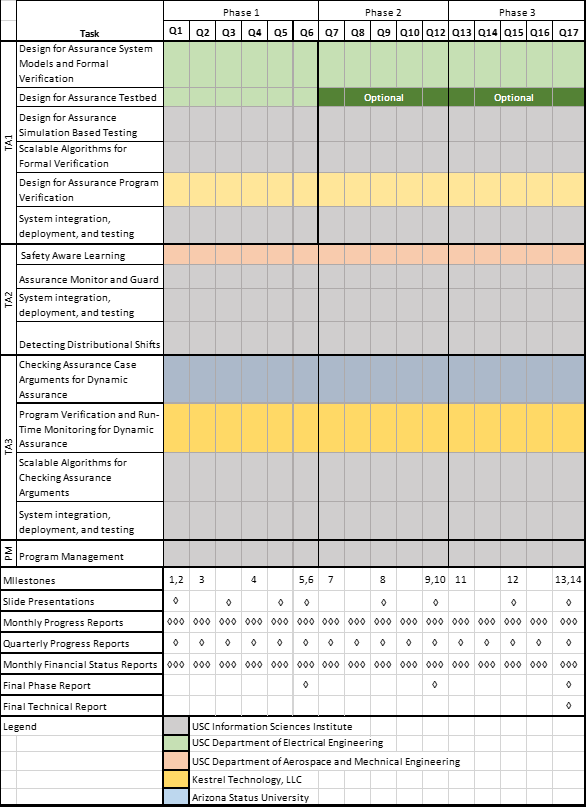
\includegraphics[width=.95\textwidth]{figs/Safeguard_Schedule_V6}
\end{center}
\vspace{-.2in}\caption{Project schedule along with a summary of milestones.  The legend maps task color to organization primary responsible for the task. } 
\label{fig:sandm}
\end{figure}
 

% \section{Level of Effort by Task \textcolor{red}{[Mike/Lisa - 1 pages]}}

% \textcolor{blue}{
% \begin{itemize}
% \item Will be a separate spreadsheet
% \item
% \end{itemize}
% }

\section*{Appendix A: Team Members and Other Information}
\addcontentsline{toc}{section}{Appendix A: Team Members and Other Information}

\baades{This section is mandatory and must include all of the following
components. If a particular subsection is not applicable, state “NONE”.}

\vspace{1ex}

\noindent
\textbf{Team Member Identification}:

\vspace{1ex}

\baades{Provide a list of all team members including the
prime, subcontractor(s), and consultant(s), as applicable. Identify specifically
whether any are a non-US organization or individual, FFRDC and/or Government
entity.}

\begin{centering}

%\small
\begin{tabular}{|p{1.8in}|p{1in}|p{1.1in}|p{0.7in}|p{0.8in}|p{0.7in}|}
\hline
 \textbf{Name} &  \textbf{Role} & \textbf{Organization} & \textbf{Non-US Org?}  & \textbf{Non-US Ind?} &  \textbf{FFRDC or Gov} \\
 \hline
Craig A. Knoblock & Prime & USC & N & N & N\\ \hline
Michael Orosz & Prime & USC & N &  N & N \\ \hline
Satish Thittamaranahalli & Prime & USC & N &  Y & N \\ \hline
Ryan Goodfellow & Prime & USC & N &  N & N \\ \hline
Anoop Kumar & Prime & USC & N & N & N \\ \hline
Satyandra Gupta & Prime & USC & N & N & N \\ \hline
Pierluigi Nuzzo & Prime & USC & N & Y & N \\ \hline
Petros Ioannou & Prime & USC & N & N & N \\ \hline
Chitta Baral & Subcontractor & ASU & N & N & N \\ \hline
Matt Barry & Subcontractor & Kestrel Technology & N & N & N \\ \hline
Douglas Smith & Subcontractor & Kestrel Technology & N & N & N \\ \hline
Henny Sipma & Subcontractor & Kestrel Technology & N & Y & N \\ \hline
\end{tabular} 
\end{centering}

\vspace{1ex}

\noindent
\textbf{Government or FFRDC Team Member Proof of Eligibility to Propose}: NONE

\baades {If
none of the team member organizations (prime or subcontractor) are a
Government entity or FFRDC, state “NONE”.}

\vspace{1ex}

\noindent
\textbf{Government or FFRDC Team Member Statement of Unique Capability}: NONE

\vspace{1ex}

\noindent
\textbf{Organizational Conflict of Interest Affirmations and Disclosure}: NONE

\vspace{1ex}

\noindent
\textbf{Intellectual Property (IP)}: 
\baades {
If no IP restrictions are intended, state “NONE”.
The Government will assume unlimited rights to all IP not explicitly identified as
having less than unlimited rights in the proposal.
For all technical data or computer software that will be furnished to the
Government with other than unlimited rights, provide (per Section VI.B.1) a list
describing all proprietary claims to results, prototypes, deliverables or systems
supporting and/or necessary for the use of the research, results, prototypes
and/or deliverables. Provide documentation proving ownership or possession of
appropriate licensing rights to all patented inventions (or inventions for which a
patent application has been filed) to be used for the proposed project.
}
\begin{centering}

%\small
\begin{tabular}{|p{2.1in}|p{1.2in}|p{1.4in}|p{2in}|}
\hline
\multicolumn{4}{|c|}{COMMERCIAL ITEMS }\\ \hline 
 \textbf{Technical Data, Computer Software To be Furnished With Restrictions} &  \textbf{Basis for Assertion} & \textbf{Asserted Rights Category} & \textbf{Name of Person Asserting Restrictions}  \\  \hline
KT Advance & Developed with mixed funding. & Restricted & David Kulich, Contracts Manager, Kestrel technology, LLC.\\ \hline
\end{tabular} 
\end{centering}

\vspace{1ex}

\noindent
\textbf{Human Subjects Research (HSR)}: NONE

\vspace{1ex}

\noindent
\textbf{Animal Use}: NONE

\vspace{1ex}

\noindent
\textbf{Representations Regarding Unpaid Delinquent Tax Liability or a Felony
Conviction under Any Federal Law}: 
%NONE

\begin{enumerate}
\item
The proposer is  not a corporation that has any unpaid Federal tax liability that has been assessed, for which all judicial and administrative remedies have been exhausted or have lapsed, and that is not being paid in a timely manner pursuant to an agreement with the authority responsible for collecting the tax liability,
\item
The proposer is not a corporation that was convicted of a felony criminal violation under a Federal law within the preceding 24 months.
\end{enumerate}

\vspace{1ex}

\noindent
\textbf{Cost Accounting Standards (CAS) Notices and Certification}:
\baades{
For any proposer who submits a proposal which, if accepted, will result in a CAS-compliant
contract, must include a Disclosure Statement as required by 48 CFR
9903.202. The disclosure forms may be found at
http://www.whitehouse.gov/omb/procurement\_casb
If this section is not applicable, state “NONE”. For further information regarding
this subject, please see www.darpa.mil/work-with-us/additional-baa.
}
NONE


%\section{Appendix B \textcolor{red}{[No Page Count]}}

\section{References}
\bibliographystyle{acm} 
\bibliography{TA3/ta3,TA2/ta2,TA1/ta1}
\end{document}
%%\documentclass[a4paper]{article}
%\documentclass[12pt]{article}
\documentclass[12pt]{dod-blank}

%% Language and font encodings
\usepackage[english]{babel}
\usepackage[utf8x]{inputenc}
\usepackage[T1]{fontenc}

%% Sets page size and margins
%%\usepackage[a4paper,top=3cm,bottom=2cm,left=3cm,right=3cm,marginparwidth=1.75cm]{geometry}
%\usepackage[top=1in, bottom=1in, left=1in, right=1in]{geometry}



%% Useful packages
\usepackage{amsmath}
\usepackage{graphicx}
  \graphicspath{{.}{./image/}}
  \DeclareGraphicsExtensions{.png,.jpg} 
\usepackage[colorinlistoftodos]{todonotes}
\usepackage[colorlinks=true, allcolors=blue]{hyperref}
\usepackage{tabularx}
\usepackage{multirow}
\usepackage{tabulary}
\usepackage{float}
\usepackage{wrapfig}
\usepackage[export]{adjustbox}
\usepackage{comment}
\usepackage{tabularx}
\usepackage{multirow}
\usepackage{tabulary}
\usepackage{enumitem}

\usepackage{listings}
\usepackage{color}
\usepackage{array}
\usepackage{subcaption}
\usepackage{xcolor}




\renewcommand{\textfraction}{0}
\renewcommand{\topfraction}{1.0}
\renewcommand{\bottomfraction}{1.0}

\usepackage{longtable}
%% macros
\newif\iffinal
\finaltrue
\iffinal
  
    \newcommand\baareq[1]{}
    \newcommand\baades[1]{}
 
 
\else
    \definecolor{darkgreen}{rgb}{0,0.4,0}
    \definecolor{darkcyan}{rgb}{0,0.4,0.4}
    \definecolor{darkblue}{rgb}{0,0,0.5}
    
    \newcommand\baareq[1]{{\color{darkcyan}[\textbf{Requirement:} #1]}}
    \newcommand\baades[1]{{\color{darkcyan}[\textbf{Description:} #1]}}
 
\fi




\def\naive{na\"{\i}ve}



\lstset{ 
  backgroundcolor=\color{white},   % choose the background color; you must add \usepackage{color} or \usepackage{xcolor}
  basicstyle=\footnotesize\ttfamily,            % the size of the fonts that are used for the code
  breakatwhitespace=false,         % sets if automatic breaks should only happen at whitespace
  breaklines=true,                 % sets automatic line breaking
  captionpos=b,                    % sets the caption-position to bottom
  commentstyle=\color{mygreen},    % comment style
  % deletekeywords={...},            % if you want to delete keywords from the given language
  escapeinside={\%*}{*)},          % if you want to add LaTeX within your code
  extendedchars=true,              % lets you use non-ASCII characters; for 8-bits encodings only, does not work with UTF-8
  frame=single,	                   % adds a frame around the code
  keepspaces=false,                 % keeps spaces in text, useful for keeping indentation of code (possibly needs columns=flexible)
  keywordstyle=\color{blue}\bfseries\underbar,       % keyword style
  language=Prolog,                 % the language of the code
  % morekeywords={if,and},        % if you want to add more keywords to the set
  numbers=none,                    % where to put the line-numbers; possible values are (none, left, right)
  numbersep=5pt,                   % how far the line-numbers are from the code
  numberstyle=\tiny\color{mygray}, % the style that is used for the line-numbers
  rulecolor=\color{black},         % if not set, the frame-color may be changed on line-breaks within not-black text
  showspaces=false,                % show spaces everywhere adding particular underscores; it overrides 'showstringspaces'
  showstringspaces=false,          % underline spaces within strings only
  showtabs=false,                  % show tabs within strings adding particular underscores
  stepnumber=2,                    % the step between two line-numbers. If it's 1, each line will be numbered
  stringstyle=\color{mymauve},     % string literal style
  tabsize=2,	                   % sets default tabsize to 2 spaces
  title=\lstname                   % show the filename of files included with \lstinputlisting; also try caption instead of title
}

% apply trick for additional keywords for our AC DSL
\lstset{
	emph={for, if, and, or},
    emphstyle={\color{blue}\bfseries\underbar}
}




\title{DARPA Assured Autonomy}
\author{Technical Volume- \textcolor{red}{Thirty-Eight (38) pages max}}

\begin{document}
\pagenumbering{roman}
 
\begin{center}
\large{\textbf{Volume 1: Technical and Management Proposal}}
\end{center}
\textbf{BAA Number:} DARPA-HR001117S0045 \\
\textbf{Technical Area:} TA1, TA2, and TA3 \\
\textbf{Proposal Title:} Assured Autonomy for Learning Enabled Vehicles (Safeguard) \\
\textbf{Lead Institution:} University of Southern California \\
\textbf{Type of organization: } “OTHER EDUCATIONAL” \\

\begin{tabularx}{\linewidth}{XX}

 \textbf{Technical Point of Contact} &  \textbf{Administrative Point of Contact }   \\
Dr.\ Craig A. Knoblock  & Sapphire Masterson  \\ 
USC Information Sciences Institute & USC Dept. of Contracts \& Grants \\
4676 Admiralty Way, Suite 1001 & 4676 Admiralty Way, Suite 1001 \\
Marina del Rey, CA 90292 & Marina del Rey, CA 90292 \\
Tel: 310-448-8786 &  Tel: (310) 448-9161 \\
E-mail: knoblock@isi.edu  & E-mail: sapphirm@usc.edu \\
\end{tabularx}
\\
\\
\textbf{Award instrument requested:}  Procurement Contract, Cost-Reimbursement, No Fee
\\
\\
\textbf{Total amount of the proposed effort:} \$ ...\\
Phase I: \$ ... \\
Phase II: \$ ... \\
Phase III: \$ ... \\
\\
\textbf{Place(s) of performance:} USC, Marina del Rey, CA; Los Angeles, CA;  Tempe, AZ; Palo Alto, CA \\
\textbf{Period(s) of performance:} 04/02/2018 - 03/31/2022     \\
\\
\textbf{Other team members:} \\
\begin{tabularx}{\linewidth}{XX}
Kestrel Technology  & Arizona State University \\
(small business) & (Other Educational)\\
POC: Matthew Barry & POC: Chitta Baral\\
3260 Hillview Avenue & Department of Computer Science and Engr. \\
Palo Alto, CA 94304 & Ira A. Fulton School of Engineering \\ 
phone: (832)205-4876 & Arizona State University\\ 
mrbarry@kestreltechnology.com & Brickyard Suite 572, 699 S. Mill Avenue \\
& Tempe, AZ 85281-8809, U.S.A.\\
& email: chitta@asu.edu\\
\end{tabularx}
\\
\textbf{Proposal validity period: } 180 days\\
\\
\textbf{Data Universal Numbering System (DUNS) number: } 072933393\\
\textbf{Taxpayer identification number:} 95-1642394\\
\textbf{Commercial and Government Entity (CAGE) code:} 1B729 Marina del Rey, CA\\
\textbf{Proposer’s reference number (if any):}  4409-0\\

\newpage
\section{Table of Contents}
\tableofcontents

\newpage
\pagenumbering{arabic}
\section{Executive Summary}
As we rapidly move into a world where machine learning plays a central role in realizing autonomous systems, it is becoming increasingly important to develop techniques that assure that these systems will operate safely and perform as expected. Current approaches are limited to providing assurance for systems with limited or no  learning capabilities. In this context, DARPA's Assured Autonomy BAA seeks to \emph{develop rigorous design and analysis technologies for continual assurance of learning-enabled autonomous systems}. USC in collaboration with Kestrel Technology and ASU is pleased to submit a comprehensive TA1, TA2, and TA3 proposal entitled \emph{``Assured Autonomy for Learning Enabled Vehicles (Safeguard).''} We plan to provide an end-to-end solution to support autonomous systems with learning-enabled components, ranging from design technologies for assurance, to assurance monitoring and control techniques, to representation and online evaluation of assurance cases. We have assembled a strong team of experts that cover the range of technologies that are required to create such an end-to-end system. If successful, the project will provide the technologies for building the next-generation of learning-enabled autonomous systems.  The entire project will take four years and cost \textcolor{red}{\$??}, with an initial version completed at the end of Phase I and successive versions with additional capabilities and improved scalability at the end of Phase II and Phase III.  

In the remainder of this section, we first introduce an  unmanned surface vehicle scenario that will be used throughout the proposal to describe the approach.  Next, we describe our approach to design, monitoring, and dynamic assurance. Finally, we introduce the team involved in the project. 

\textbf{Motivating Scenario.} Consider an autonomous unmanned surface vehicle (USV) guarding a valuable asset in the ocean when an unknown vehicle  approaches the security perimeter, under challenging weather conditions. In this scenario, the USV is required to approach the intruding vehicle, issue a warning signal, and escort it to a safe distance from the controlled area. However, as the USV has no a priori knowledge of its external environment behaviors (e.g., water depth, waves, wind, current, visibility), pre-computing a feasible trajectory, let alone optimal, becomes a non-trivial problem. For trajectory planning, the USV must continuously perform the following tasks:
\begin{itemize}[itemsep=0pt,leftmargin=*]
 \item Sense the current state of the surrounding environment (e.g., water depth, waves, wind, current, visibility) and estimate its own maneuverability constraints (e.g., braking distance, available acceleration, maximum velocity, turning radius, turning rate, safety distance) based on the state of the environment;      
\item Sense the static obstacles in the sensor range and generate a traversability map;
\item Sense the moving obstacles and classify them;   
\item Predict future trajectories of moving obstacles; 
\item Determine if any of the COLREGS \cite{commandant1999international} rules will be in effect with respect to one or more of the nearby vessels and identify the vessels with the right of way.    
\end{itemize}
The above information will be used by the trajectory planner to compute an initial trajectory, which will be continuously refined as the USV gathers additional information.
% It is not possible for the USV to be tested in every possible environment. 
The USV will use learning enabled components to take  decisions as it encounters new situations, such as  
\begin{itemize}[itemsep=0pt,leftmargin=*]
\item Classifiers to identify moving obstacles based on physical appearance and motion signatures,
\item Algorithms to estimate the sensor capabilities in adverse weather conditions,   
\item Algorithms to accurately estimate uncertainty in the environment, 
\item Classifiers to generate traversability maps,
\item Prediction of external vessel behaviors based on motion histories, 
\item Reinforcement learning  to ensure COLREGS compliance of maneuvers,  
\item Algorithms to learning pursuit behaviors.  
\end{itemize}
Learning enabled components will interact with each other in complex ways, where a misclassification error in one component may eventually compromise the entire mission.   
% We will need to make sure that each learning enabled components has a run-time monitor that will ensure that the assumptions made by the learning-enabled component remain valid and prevent erroneous learning. 
% For example, if the vehicle is exhibiting significant error in trajectory tracking, then simply downgrading the trajectory tracking error value may not be a good option.  The failure of prediction of trajectory tracking error might be due to the presence of a significant wake caused by a nearby vessel. The presence of the nearby vessel can be used to explain the degradation in trajectory tracking performance. As the vessel moves away, we can expect the trajectory tracking performance to return to the predicted level.  
While exhaustive validation of learning-enabled cyber-physical systems (LE-CPSs) is a prohibitive task~\cite{Kalra16},
their complexity, heterogeneity, and highly dynamic nature
make it challenging to even leverage existing model-based development techniques to effectively assess system correctness 
% dependability, 
at design time or enforce it at runtime.

\textbf{Design for Assurance.} Safeguard uses a platform-based design approach~\cite{Nuzzo15b} to organize the design process for a LE-CPS and to build assurance cases. Composite models are developed at several levels of abstraction,
from top-level system requirements and safety constraints down to the
implementation level.  Intermediate levels add detail to the levels
above.  The different levels are connected by refinement mappings that
allow properties established at one level to be preserved at the next
level (see Figures~\ref{fig:methodology} and~\ref{fig:assurance}).

Contracts are used to formally specify components and composite models
in terms of (1) Assumptions -- the assumed behaviors of the
environment and the behaviors of other components, and (2) Guarantees
-- the behavior properties that a model guarantees if it operates in a
context that satisfies its assumptions.  A calculus of contracts
allows horizontal composition of contracts to generate contracts for
composite models.  Vertical contracts are used to specify the mapping
or refinement relation between models at different levels of
abstraction.  The system design process starts with a high-level
contract that expresses overall system assumptions and requirements.
Subsequent levels express models with increasing detail until the
lowest level expresses the system in terms of hardware components and
their software controllers.

The assurance case for a CPS arises from the horizontal and vertical
structure of the design in several ways.  The components used within a
particular level are either (1) synthesized using
correct-by-construction design tools together with proofs, (2) derived
statically or dynamically using safety-aware machine-learning
techniques, (3) written manually and verified by analysis tools, or
(4) written manually and validated by extensive testing.  The
assurance case for the whole reflects its compositional structure.  We
anticipate that well-specified contracts together with the calculus of
contracts will eliminate well-known problems with unexpected emergent
behaviors in CPS systems.

The assurance case for the lowest-layer design arises from both the
intra-level assurance and from properties and their proofs that are
preserved under the refinement mapping from the top-level
requirements.  The refinement mappings between model layers will be
constructed using a variety of techniques.  A contract at an abstract
level can be mapped to a component or refined contract by (1)
retrieval of pre-verified components from a platform library, (2)
synthesis using correct-by-construction design and optimization tools,
or (3) manual coding to satisfy a contract.  The mapping of a
composite model will be composed from the mappings of its constituent
components or contracts.  When a composite model cannot be mapped
compositionally to the next level, it will be generated using
correct-by-construction design and optimization tools.

\textbf{Assurance Monitoring and Control.}
We provide an integrated framework for safety-aware learning, assurance monitoring and control, detecting distribution shifts. Three major components offer an efficient TA2 architecture as well as interfaces with TA1 and TA3, that is, (a) safety-aware learning and planning, (b) assurance monitors for guarding architectural and safety constraints; and (c) distribution shift detection.

We will develop a new learning-enabled online decision-making framework that allows opportunistically composing a sequence of actions (maneuvers) to reduce uncertainty in the system capability model without suspending the progress toward the mission goals or compromising safety. Each candidate action is evaluated based on three criteria: (1) the risk of violating a safety constraint using the current uncertainties in the parameter estimates; (2) its relevance to the mission goals; (3)  its expected information gain, i.e., reduction in uncertainty, with respect to the parameter estimates. These evaluations are combined to produce a cumulative mission utility value for each action that drives our learning-enabled decision-making framework. The problem of generating and evaluating sequences of actions can be posed in several way. For example, it can be solved using a branch-and-bound search method like Anytime A*, or formulated with the finite-horizon Markov Decision Process (MDP) framework. We will develop new scalable search strategies to solve this problem efficiently, by potentially evaluating a recent method developed at USC, called FastMap, that can significantly improve the execution time. 

We will develop monitors for architectural and safety constraints. 
% While these constraints can be checked over and over again as sensor information flow in, this naive strategy accounts for a lot of computational overhead. 
To achieve scalability and decrease the overhead, we propose the application of a technique that we currently use in DARPA's RSPACE program, which leverages a physical model of the vehicles dynamics and its interactions with the environment to efficiently determine the readout frequency. We propose two  extensions of this basic idea. First, we will use the theory of Variable Elimination to prioritize which variables to monitor, e.g., controllable, versus uncontrollable, adversarially controlled, or unobservable variables. Second, we invoke the dynamic assessment of assurance cases only when needed. This  decreases the number of times dynamic assessment of assurance cases is initiated as well as the communication bandwidth between the TA2 and TA3 components.

Finally, we will identify a distribution shift by combining statistical and machine learning techniques to differentiate between environmental and sensor changes. We will exploit a categorization of the shifts based on their cause and duration as well as extend our earlier work on detecting and mitigating sensor failures for all types of monitored variables.  

\textbf{Dynamic Assurance:} The Safeguard {\em design for assurance\/} activity takes a systems-theoretic stance toward safety.  Consequently, it presumes that safety is an emergent property of the system, and that hazards can present themselves through unintended interactions and performance violations in addition to causal events such as component failures.  Our design approach includes consideration of intent as well as hazard analysis and mitigation.  The artifacts from these activities populate contracts and assumptions for the dynamic assurance case.  
We thus build safety into the product by working at a systems-level viewpoint, using lexicon and design patterns familiar to both hardware and software engineers; safety is an emergent property of the system, not an afterthought.  
As system behavior evolves during runtime owing to learning, threats, degradation, or some other factor, the dynamic assurance case identifies whether the safety constraints continue to be satisfied.  If not, it provides notifications or issues recovery instructions directly from a lookup table.

Our implementation of the dynamic assurance case employs a declarative knowledge base inference engine and a domain-specific language tailored to our approach.  We have used them successfully for assurance case tool sets and arguments, and will extend them to reason about uncertainty and learning.  Our approach to achieve scalability is to specialize solvers toward modularity and to take advantage of domain knowledge.  Specifically, we will develop answer set programming techniques for context-dependent learning for reasoning about the learning-enabled components as well as learning assurance rules.  We will develop new formalisms for uncertainty to include causality, using weights for computing probabilities, and probabilistic non-monotonicity.  To achieve scaling objectives we will implement specializations using modularity, weighted CSPs, and message passing. 

% The system safety constraints revealed from that design become the key elements of our dynamic assurance case.  Our verification tools ensure the constraints are relevant, identifiable, and their implementation and effect observable.  

\textbf{Team.} We have assembled a team that is exceptionally well-qualified to build the proposed Safeguard system.  The team will be led by Dr.\ Craig Knoblock, the Principal Investigator for the effort, who currently leads the Intelligent Systems Division at the Information Sciences Institute.  He has led many large DARPA and IARPA projects over the years and has a strong track record in conducting leading edge research and then transitioning the technology to commercial use.  He will be supported by Dr.\ Michael Orosz as the Project Manager, who also has  experience in managing large research projects and on autonomous systems.  The TA1 team will be led by Dr.\ Pierluigi Nuzzo, who is an expert in embedded system design methodologies and the  application of formal methods to cyber-physical systems.  The TA1 team also includes Dr.\ Doug Smith, who has spent many years working on scalable correct-by-construction techniques and Dr.\ Henny Sipma, who has significant experience in applying program verification methods to real-world problems.  The TA1 team also includes Ryan Goodfellow, who has done a large amount of work on simulation-based testing.  The TA2 team will be led by Dr.\ Knoblock who has worked on topics related to both monitoring and detecting distribution changes.  He will be supported by Dr.\ Satyandra Gupta, who is an expert on autonomous surface vehicles as well as on safety-aware learning. He will also be supported by Drs.\ Anoop Kumar and Satish Thittamaranahalli, who have also previously worked on efficient methods for execution monitoring.  The TA3 team will be lead by Dr.\ Matthew Barry, who has experience in creating the technologies for assurance cases.  He will be supported by Dr.\ Chitta Baral, who is an expert on ASP solvers and by Dr.\ Thittamaranahalli who is an expert on SAT solvers, both of which will be applied to provide scalable assurance case reasoning.  Finally, Dr.\ Petros Ioannou, who is an expert on control systems for autonomous vehicles will provide an autonomous vehicle platform, which will form the focus of our work until the TA4 teams provide additional vehicle platforms for development.  

\newpage
\section{Innovative Claims and Deliverables}

In this project we will develop and build an end-to-end system for assured autonomy.  This section describes the key innovations by technical area and then the overall deliverables of the project.

\paragraph{Design for Assurance}

\begin{itemize}[itemsep=0pt,leftmargin=*]
\item We address the LE-CPS design challenges via a holistic approach that can contextually generate design artifacts and assurance cases. We develop a compositional, contract-based modeling framework, methods, and tools to support the design process from system-level requirement capture,  formalization, and analysis, to the generation, testing, and continual monitoring of software and hardware artifacts in feedback loop with a physical process.

\item We develop compositional abstractions and interfaces (vertical contracts) that can  bridge heterogeneous formalisms and heterogeneous decomposition architectures to make system analysis and synthesis tractable, consistently combine different verification and synthesis methods at design time, and provide seamless support for dynamic assurance at run time. %We aim to quantitatively capture the confidence in the satisfaction of requirements under uncertain or unknown conditions, and resilience properties of  systems at different abstraction levels, to enable trade-off evaluation between resilience, performance, and cost.

\item We develop a unifying framework and efficient algorithms to reason about the combination of discrete and continuous dynamics and constraints in the presence of uncertainties in LE-CPS using a satisfiability modulo convex approach~\cite{Shoukry2017} for contract-based system verification and scalable trajectory planning.  

\item We provide an environment for high-fidelity CPS testing, in which production-ready software, e.g.,  safety-critical learning and control, may be deployed and tested 
% by extending the Cypress testbed environment \cite{Goodfellow2015Cypress:Systems} 
with time dilation facilities, so that it synchronizes with a physical simulation that is not necessarily running in real time, while still having the perception of real time.

\item We 
% These facilities allow a cyber system to be  
propose an approach for unanticipated behavior space identification and test coverage maximization which leverages results from the theory of differential algebraic equation (DAE)~\cite{Berger2013ControllabilitySurvey,Ilchmann2005ATheory,BergerOnSystems,Lamour2013} 
to prune the behavior search space and identify smaller regions of interest for efficient simulation-based testing. 
% We then compute the intersection of these two behavior spaces and restrict our simulation based testing search space to this subspace.
\end{itemize}

\paragraph{Assurance Monitoring and Control}

\begin{itemize}[itemsep=0pt,leftmargin=*]
\item 
%We integrate safety-aware learning into the overall decision making problem. The goal is to maximize mission utility without violating the safety constraints. 
Our safety-aware learning framework enables the system to opportunistically select and execute actions to assist the learning-enabled component in reducing model uncertainty without compromising safety or deviating from the mission goals. The value of uncertainty reduction is explicitly incorporated in the optimization process for selecting the best action.  
\item For safety-aware learning, we propose the idea of preprocessing the search space of the problem domain before queries and observations come in. With such a linear-time preprocessing phase, the performance of search and optimization algorithms can be significantly boosted. For example, in regular A* search, the intensional or extensional search space can be preprocessed in near-linear time to yield an embedding of each state as a point in Euclidean space~\cite{cujakk}. Then, when the query comes in, A* search can make use of these Euclidean distances as heuristic distances between two states to yield order-of-magnitude speedups. 
%In Anytime A* for safety-aware learning and planning, this leads to a significantly better quality of actions chosen within a time limit, and in the MDP framework, the same ideas can be used to improve the convergence of Bellman updates for safety-aware Reinforcement Learning.
\item As massive amounts of sensor information flow in, it is imperative for us to efficiently process this information for monitoring architectural and safety constraints. Building on our past work on similar tasks, we propose novel technologies for efficiently monitoring constraints. These algorithms can yield an exponential reduction in the amount of sensor data that needs to be processed. Doing this also reduces the message complexities between the various modules. %We also propose to use the theory of Variable Elimination (VE) to monitor constraints with uncontrollable, adversarially controlled, and/or unobservable variables. VE yields a substrate constraint to monitor that characterizes a dominant strategy of the controllable variables over the uncontrollable, adversarially controlled, and/or unobservable variables.
\item We will develop techniques to identify  distributional shifts and determine the underlying cause (e.g., change in environment, sensor failure,   etc.), as well as strategies for handling the various distributional shifts.   Notably, we propose to build on our past work and use compact representations to exploit historical data to identify distributional shifts.
\end{itemize}

\paragraph{Dynamic Assurance}

\begin{itemize}[itemsep=0pt,leftmargin=*]

\item We demonstrate the integration of dynamic assurance for safety-critical learning-enabled dynamic systems in which evolutionary behaviors are expected and tolerated as a property of the functionality.   The impact will be consequential contributions safety-critical dynamic systems in which evolutionary behaviors are expected and tolerated as portion of the functionality.   
\item We implement dynamic assurance by combining features of system safety, formal methods, logic programming, uncertain reasoning, and domain-specific languages.  We populate assurance case arguments at several levels of modeling and implementation abstraction, using the analysis results to produce design-time evidence supporting assurance claims.  
%We provide automated reasoning about the assurance case itself to produce verification, consistency, and completeness results for the argument.  Dynamic assurance results then yield trusted explanations of whether safety constraints and assumptions and other contracts still hold during the collection of runtime evidence from monitors. 
\item We develop and demonstrate ASP formalisms crucial to applications in dynamic assurance. We demonstrate the suitability of the technology especially for assurance case arguments owing to the improved legibility, consistency and completeness checks, handling of uncertain and default reasoning, and scalability.  
%We will produce modularized solvers for enhanced performance based on recent algorithmic developments in exploiting structure, kernelization, and message passing. We provide a formalism to enable learning of assurance rules. 
We provide a novel approach to handling uncertainty that provides the ability to do causal and counter-factual reasoning as well as probabilistic non-monotonicity.  Overcoming limitations of traditional inductive logic techniques, we develop a novel iterative and incremental approach based on context dependent learning. 
\end{itemize}

\paragraph{Deliverables}
During the course of this project, we will build and deliver a fully-operational system that covers all three of the technical areas.  The detailed capabilities of this system are described in the individual technical sections.  The resulting system will be available as open source under a permissive license, which will allow other organizations to use the work, extend it in new directions, and even commercialize the software.  Kestrel Technology has significant experience in this space and has built and applied these types of technologies to a variety of real world tasks.  Kestrel is ideally suited to pursue commercial uses of this technology and the permissive license will facilitate exploring these opportunities since there will be no need to negotiate intellectual property rights.  

\newpage
\section{Technical Plan}
%%\documentclass[a4paper]{article}
%\documentclass[12pt]{article}
\documentclass[12pt]{dod-blank}

%% Language and font encodings
\usepackage[english]{babel}
\usepackage[utf8x]{inputenc}
\usepackage[T1]{fontenc}

%% Sets page size and margins
%%\usepackage[a4paper,top=3cm,bottom=2cm,left=3cm,right=3cm,marginparwidth=1.75cm]{geometry}
%\usepackage[top=1in, bottom=1in, left=1in, right=1in]{geometry}



%% Useful packages
\usepackage{amsmath}
\usepackage{graphicx}
  \graphicspath{{.}{./image/}}
  \DeclareGraphicsExtensions{.png,.jpg} 
\usepackage[colorinlistoftodos]{todonotes}
\usepackage[colorlinks=true, allcolors=blue]{hyperref}
\usepackage{tabularx}
\usepackage{multirow}
\usepackage{tabulary}
\usepackage{float}
\usepackage{wrapfig}
\usepackage[export]{adjustbox}
\usepackage{comment}
\usepackage{tabularx}
\usepackage{multirow}
\usepackage{tabulary}
\usepackage{enumitem}

\usepackage{listings}
\usepackage{color}
\usepackage{array}
\usepackage{subcaption}
\usepackage{xcolor}




\renewcommand{\textfraction}{0}
\renewcommand{\topfraction}{1.0}
\renewcommand{\bottomfraction}{1.0}

\usepackage{longtable}
%% macros
\newif\iffinal
\finaltrue
\iffinal
  
    \newcommand\baareq[1]{}
    \newcommand\baades[1]{}
 
 
\else
    \definecolor{darkgreen}{rgb}{0,0.4,0}
    \definecolor{darkcyan}{rgb}{0,0.4,0.4}
    \definecolor{darkblue}{rgb}{0,0,0.5}
    
    \newcommand\baareq[1]{{\color{darkcyan}[\textbf{Requirement:} #1]}}
    \newcommand\baades[1]{{\color{darkcyan}[\textbf{Description:} #1]}}
 
\fi




\def\naive{na\"{\i}ve}



\lstset{ 
  backgroundcolor=\color{white},   % choose the background color; you must add \usepackage{color} or \usepackage{xcolor}
  basicstyle=\footnotesize\ttfamily,            % the size of the fonts that are used for the code
  breakatwhitespace=false,         % sets if automatic breaks should only happen at whitespace
  breaklines=true,                 % sets automatic line breaking
  captionpos=b,                    % sets the caption-position to bottom
  commentstyle=\color{mygreen},    % comment style
  % deletekeywords={...},            % if you want to delete keywords from the given language
  escapeinside={\%*}{*)},          % if you want to add LaTeX within your code
  extendedchars=true,              % lets you use non-ASCII characters; for 8-bits encodings only, does not work with UTF-8
  frame=single,	                   % adds a frame around the code
  keepspaces=false,                 % keeps spaces in text, useful for keeping indentation of code (possibly needs columns=flexible)
  keywordstyle=\color{blue}\bfseries\underbar,       % keyword style
  language=Prolog,                 % the language of the code
  % morekeywords={if,and},        % if you want to add more keywords to the set
  numbers=none,                    % where to put the line-numbers; possible values are (none, left, right)
  numbersep=5pt,                   % how far the line-numbers are from the code
  numberstyle=\tiny\color{mygray}, % the style that is used for the line-numbers
  rulecolor=\color{black},         % if not set, the frame-color may be changed on line-breaks within not-black text
  showspaces=false,                % show spaces everywhere adding particular underscores; it overrides 'showstringspaces'
  showstringspaces=false,          % underline spaces within strings only
  showtabs=false,                  % show tabs within strings adding particular underscores
  stepnumber=2,                    % the step between two line-numbers. If it's 1, each line will be numbered
  stringstyle=\color{mymauve},     % string literal style
  tabsize=2,	                   % sets default tabsize to 2 spaces
  title=\lstname                   % show the filename of files included with \lstinputlisting; also try caption instead of title
}

% apply trick for additional keywords for our AC DSL
\lstset{
	emph={for, if, and, or},
    emphstyle={\color{blue}\bfseries\underbar}
}




\title{DARPA Assured Autonomy}
\author{Technical Volume- \textcolor{red}{Thirty-Eight (38) pages max}}

\begin{document}
\pagenumbering{roman}
\include{cover}

\newpage
\section{Table of Contents}
\tableofcontents

\newpage
\pagenumbering{arabic}
\section{Executive Summary}
As we rapidly move into a world where machine learning plays a central role in realizing autonomous systems, it is becoming increasingly important to develop techniques that assure that these systems will operate safely and perform as expected. Current approaches are limited to providing assurance for systems with limited or no  learning capabilities. In this context, DARPA's Assured Autonomy BAA seeks to \emph{develop rigorous design and analysis technologies for continual assurance of learning-enabled autonomous systems}. USC in collaboration with Kestrel Technology and ASU is pleased to submit a comprehensive TA1, TA2, and TA3 proposal entitled \emph{``Assured Autonomy for Learning Enabled Vehicles (Safeguard).''} We plan to provide an end-to-end solution to support autonomous systems with learning-enabled components, ranging from design technologies for assurance, to assurance monitoring and control techniques, to representation and online evaluation of assurance cases. We have assembled a strong team of experts that cover the range of technologies that are required to create such an end-to-end system. If successful, the project will provide the technologies for building the next-generation of learning-enabled autonomous systems.  The entire project will take four years and cost \textcolor{red}{\$??}, with an initial version completed at the end of Phase I and successive versions with additional capabilities and improved scalability at the end of Phase II and Phase III.  

In the remainder of this section, we first introduce an  unmanned surface vehicle scenario that will be used throughout the proposal to describe the approach.  Next, we describe our approach to design, monitoring, and dynamic assurance. Finally, we introduce the team involved in the project. 

\textbf{Motivating Scenario.} Consider an autonomous unmanned surface vehicle (USV) guarding a valuable asset in the ocean when an unknown vehicle  approaches the security perimeter, under challenging weather conditions. In this scenario, the USV is required to approach the intruding vehicle, issue a warning signal, and escort it to a safe distance from the controlled area. However, as the USV has no a priori knowledge of its external environment behaviors (e.g., water depth, waves, wind, current, visibility), pre-computing a feasible trajectory, let alone optimal, becomes a non-trivial problem. For trajectory planning, the USV must continuously perform the following tasks:
\begin{itemize}[itemsep=0pt,leftmargin=*]
 \item Sense the current state of the surrounding environment (e.g., water depth, waves, wind, current, visibility) and estimate its own maneuverability constraints (e.g., braking distance, available acceleration, maximum velocity, turning radius, turning rate, safety distance) based on the state of the environment;      
\item Sense the static obstacles in the sensor range and generate a traversability map;
\item Sense the moving obstacles and classify them;   
\item Predict future trajectories of moving obstacles; 
\item Determine if any of the COLREGS \cite{commandant1999international} rules will be in effect with respect to one or more of the nearby vessels and identify the vessels with the right of way.    
\end{itemize}
The above information will be used by the trajectory planner to compute an initial trajectory, which will be continuously refined as the USV gathers additional information.
% It is not possible for the USV to be tested in every possible environment. 
The USV will use learning enabled components to take  decisions as it encounters new situations, such as  
\begin{itemize}[itemsep=0pt,leftmargin=*]
\item Classifiers to identify moving obstacles based on physical appearance and motion signatures,
\item Algorithms to estimate the sensor capabilities in adverse weather conditions,   
\item Algorithms to accurately estimate uncertainty in the environment, 
\item Classifiers to generate traversability maps,
\item Prediction of external vessel behaviors based on motion histories, 
\item Reinforcement learning  to ensure COLREGS compliance of maneuvers,  
\item Algorithms to learning pursuit behaviors.  
\end{itemize}
Learning enabled components will interact with each other in complex ways, where a misclassification error in one component may eventually compromise the entire mission.   
% We will need to make sure that each learning enabled components has a run-time monitor that will ensure that the assumptions made by the learning-enabled component remain valid and prevent erroneous learning. 
% For example, if the vehicle is exhibiting significant error in trajectory tracking, then simply downgrading the trajectory tracking error value may not be a good option.  The failure of prediction of trajectory tracking error might be due to the presence of a significant wake caused by a nearby vessel. The presence of the nearby vessel can be used to explain the degradation in trajectory tracking performance. As the vessel moves away, we can expect the trajectory tracking performance to return to the predicted level.  
While exhaustive validation of learning-enabled cyber-physical systems (LE-CPSs) is a prohibitive task~\cite{Kalra16},
their complexity, heterogeneity, and highly dynamic nature
make it challenging to even leverage existing model-based development techniques to effectively assess system correctness 
% dependability, 
at design time or enforce it at runtime.

\textbf{Design for Assurance.} Safeguard uses a platform-based design approach~\cite{Nuzzo15b} to organize the design process for a LE-CPS and to build assurance cases. Composite models are developed at several levels of abstraction,
from top-level system requirements and safety constraints down to the
implementation level.  Intermediate levels add detail to the levels
above.  The different levels are connected by refinement mappings that
allow properties established at one level to be preserved at the next
level (see Figures~\ref{fig:methodology} and~\ref{fig:assurance}).

Contracts are used to formally specify components and composite models
in terms of (1) Assumptions -- the assumed behaviors of the
environment and the behaviors of other components, and (2) Guarantees
-- the behavior properties that a model guarantees if it operates in a
context that satisfies its assumptions.  A calculus of contracts
allows horizontal composition of contracts to generate contracts for
composite models.  Vertical contracts are used to specify the mapping
or refinement relation between models at different levels of
abstraction.  The system design process starts with a high-level
contract that expresses overall system assumptions and requirements.
Subsequent levels express models with increasing detail until the
lowest level expresses the system in terms of hardware components and
their software controllers.

The assurance case for a CPS arises from the horizontal and vertical
structure of the design in several ways.  The components used within a
particular level are either (1) synthesized using
correct-by-construction design tools together with proofs, (2) derived
statically or dynamically using safety-aware machine-learning
techniques, (3) written manually and verified by analysis tools, or
(4) written manually and validated by extensive testing.  The
assurance case for the whole reflects its compositional structure.  We
anticipate that well-specified contracts together with the calculus of
contracts will eliminate well-known problems with unexpected emergent
behaviors in CPS systems.

The assurance case for the lowest-layer design arises from both the
intra-level assurance and from properties and their proofs that are
preserved under the refinement mapping from the top-level
requirements.  The refinement mappings between model layers will be
constructed using a variety of techniques.  A contract at an abstract
level can be mapped to a component or refined contract by (1)
retrieval of pre-verified components from a platform library, (2)
synthesis using correct-by-construction design and optimization tools,
or (3) manual coding to satisfy a contract.  The mapping of a
composite model will be composed from the mappings of its constituent
components or contracts.  When a composite model cannot be mapped
compositionally to the next level, it will be generated using
correct-by-construction design and optimization tools.

\textbf{Assurance Monitoring and Control.}
We provide an integrated framework for safety-aware learning, assurance monitoring and control, detecting distribution shifts. Three major components offer an efficient TA2 architecture as well as interfaces with TA1 and TA3, that is, (a) safety-aware learning and planning, (b) assurance monitors for guarding architectural and safety constraints; and (c) distribution shift detection.

We will develop a new learning-enabled online decision-making framework that allows opportunistically composing a sequence of actions (maneuvers) to reduce uncertainty in the system capability model without suspending the progress toward the mission goals or compromising safety. Each candidate action is evaluated based on three criteria: (1) the risk of violating a safety constraint using the current uncertainties in the parameter estimates; (2) its relevance to the mission goals; (3)  its expected information gain, i.e., reduction in uncertainty, with respect to the parameter estimates. These evaluations are combined to produce a cumulative mission utility value for each action that drives our learning-enabled decision-making framework. The problem of generating and evaluating sequences of actions can be posed in several way. For example, it can be solved using a branch-and-bound search method like Anytime A*, or formulated with the finite-horizon Markov Decision Process (MDP) framework. We will develop new scalable search strategies to solve this problem efficiently, by potentially evaluating a recent method developed at USC, called FastMap, that can significantly improve the execution time. 

We will develop monitors for architectural and safety constraints. 
% While these constraints can be checked over and over again as sensor information flow in, this naive strategy accounts for a lot of computational overhead. 
To achieve scalability and decrease the overhead, we propose the application of a technique that we currently use in DARPA's RSPACE program, which leverages a physical model of the vehicles dynamics and its interactions with the environment to efficiently determine the readout frequency. We propose two  extensions of this basic idea. First, we will use the theory of Variable Elimination to prioritize which variables to monitor, e.g., controllable, versus uncontrollable, adversarially controlled, or unobservable variables. Second, we invoke the dynamic assessment of assurance cases only when needed. This  decreases the number of times dynamic assessment of assurance cases is initiated as well as the communication bandwidth between the TA2 and TA3 components.

Finally, we will identify a distribution shift by combining statistical and machine learning techniques to differentiate between environmental and sensor changes. We will exploit a categorization of the shifts based on their cause and duration as well as extend our earlier work on detecting and mitigating sensor failures for all types of monitored variables.  

\textbf{Dynamic Assurance:} The Safeguard {\em design for assurance\/} activity takes a systems-theoretic stance toward safety.  Consequently, it presumes that safety is an emergent property of the system, and that hazards can present themselves through unintended interactions and performance violations in addition to causal events such as component failures.  Our design approach includes consideration of intent as well as hazard analysis and mitigation.  The artifacts from these activities populate contracts and assumptions for the dynamic assurance case.  
We thus build safety into the product by working at a systems-level viewpoint, using lexicon and design patterns familiar to both hardware and software engineers; safety is an emergent property of the system, not an afterthought.  
As system behavior evolves during runtime owing to learning, threats, degradation, or some other factor, the dynamic assurance case identifies whether the safety constraints continue to be satisfied.  If not, it provides notifications or issues recovery instructions directly from a lookup table.

Our implementation of the dynamic assurance case employs a declarative knowledge base inference engine and a domain-specific language tailored to our approach.  We have used them successfully for assurance case tool sets and arguments, and will extend them to reason about uncertainty and learning.  Our approach to achieve scalability is to specialize solvers toward modularity and to take advantage of domain knowledge.  Specifically, we will develop answer set programming techniques for context-dependent learning for reasoning about the learning-enabled components as well as learning assurance rules.  We will develop new formalisms for uncertainty to include causality, using weights for computing probabilities, and probabilistic non-monotonicity.  To achieve scaling objectives we will implement specializations using modularity, weighted CSPs, and message passing. 

% The system safety constraints revealed from that design become the key elements of our dynamic assurance case.  Our verification tools ensure the constraints are relevant, identifiable, and their implementation and effect observable.  

\textbf{Team.} We have assembled a team that is exceptionally well-qualified to build the proposed Safeguard system.  The team will be led by Dr.\ Craig Knoblock, the Principal Investigator for the effort, who currently leads the Intelligent Systems Division at the Information Sciences Institute.  He has led many large DARPA and IARPA projects over the years and has a strong track record in conducting leading edge research and then transitioning the technology to commercial use.  He will be supported by Dr.\ Michael Orosz as the Project Manager, who also has  experience in managing large research projects and on autonomous systems.  The TA1 team will be led by Dr.\ Pierluigi Nuzzo, who is an expert in embedded system design methodologies and the  application of formal methods to cyber-physical systems.  The TA1 team also includes Dr.\ Doug Smith, who has spent many years working on scalable correct-by-construction techniques and Dr.\ Henny Sipma, who has significant experience in applying program verification methods to real-world problems.  The TA1 team also includes Ryan Goodfellow, who has done a large amount of work on simulation-based testing.  The TA2 team will be led by Dr.\ Knoblock who has worked on topics related to both monitoring and detecting distribution changes.  He will be supported by Dr.\ Satyandra Gupta, who is an expert on autonomous surface vehicles as well as on safety-aware learning. He will also be supported by Drs.\ Anoop Kumar and Satish Thittamaranahalli, who have also previously worked on efficient methods for execution monitoring.  The TA3 team will be lead by Dr.\ Matthew Barry, who has experience in creating the technologies for assurance cases.  He will be supported by Dr.\ Chitta Baral, who is an expert on ASP solvers and by Dr.\ Thittamaranahalli who is an expert on SAT solvers, both of which will be applied to provide scalable assurance case reasoning.  Finally, Dr.\ Petros Ioannou, who is an expert on control systems for autonomous vehicles will provide an autonomous vehicle platform, which will form the focus of our work until the TA4 teams provide additional vehicle platforms for development.  

\newpage
\section{Innovative Claims and Deliverables}

In this project we will develop and build an end-to-end system for assured autonomy.  This section describes the key innovations by technical area and then the overall deliverables of the project.

\paragraph{Design for Assurance}

\begin{itemize}[itemsep=0pt,leftmargin=*]
\item We address the LE-CPS design challenges via a holistic approach that can contextually generate design artifacts and assurance cases. We develop a compositional, contract-based modeling framework, methods, and tools to support the design process from system-level requirement capture,  formalization, and analysis, to the generation, testing, and continual monitoring of software and hardware artifacts in feedback loop with a physical process.

\item We develop compositional abstractions and interfaces (vertical contracts) that can  bridge heterogeneous formalisms and heterogeneous decomposition architectures to make system analysis and synthesis tractable, consistently combine different verification and synthesis methods at design time, and provide seamless support for dynamic assurance at run time. %We aim to quantitatively capture the confidence in the satisfaction of requirements under uncertain or unknown conditions, and resilience properties of  systems at different abstraction levels, to enable trade-off evaluation between resilience, performance, and cost.

\item We develop a unifying framework and efficient algorithms to reason about the combination of discrete and continuous dynamics and constraints in the presence of uncertainties in LE-CPS using a satisfiability modulo convex approach~\cite{Shoukry2017} for contract-based system verification and scalable trajectory planning.  

\item We provide an environment for high-fidelity CPS testing, in which production-ready software, e.g.,  safety-critical learning and control, may be deployed and tested 
% by extending the Cypress testbed environment \cite{Goodfellow2015Cypress:Systems} 
with time dilation facilities, so that it synchronizes with a physical simulation that is not necessarily running in real time, while still having the perception of real time.

\item We 
% These facilities allow a cyber system to be  
propose an approach for unanticipated behavior space identification and test coverage maximization which leverages results from the theory of differential algebraic equation (DAE)~\cite{Berger2013ControllabilitySurvey,Ilchmann2005ATheory,BergerOnSystems,Lamour2013} 
to prune the behavior search space and identify smaller regions of interest for efficient simulation-based testing. 
% We then compute the intersection of these two behavior spaces and restrict our simulation based testing search space to this subspace.
\end{itemize}

\paragraph{Assurance Monitoring and Control}

\begin{itemize}[itemsep=0pt,leftmargin=*]
\item 
%We integrate safety-aware learning into the overall decision making problem. The goal is to maximize mission utility without violating the safety constraints. 
Our safety-aware learning framework enables the system to opportunistically select and execute actions to assist the learning-enabled component in reducing model uncertainty without compromising safety or deviating from the mission goals. The value of uncertainty reduction is explicitly incorporated in the optimization process for selecting the best action.  
\item For safety-aware learning, we propose the idea of preprocessing the search space of the problem domain before queries and observations come in. With such a linear-time preprocessing phase, the performance of search and optimization algorithms can be significantly boosted. For example, in regular A* search, the intensional or extensional search space can be preprocessed in near-linear time to yield an embedding of each state as a point in Euclidean space~\cite{cujakk}. Then, when the query comes in, A* search can make use of these Euclidean distances as heuristic distances between two states to yield order-of-magnitude speedups. 
%In Anytime A* for safety-aware learning and planning, this leads to a significantly better quality of actions chosen within a time limit, and in the MDP framework, the same ideas can be used to improve the convergence of Bellman updates for safety-aware Reinforcement Learning.
\item As massive amounts of sensor information flow in, it is imperative for us to efficiently process this information for monitoring architectural and safety constraints. Building on our past work on similar tasks, we propose novel technologies for efficiently monitoring constraints. These algorithms can yield an exponential reduction in the amount of sensor data that needs to be processed. Doing this also reduces the message complexities between the various modules. %We also propose to use the theory of Variable Elimination (VE) to monitor constraints with uncontrollable, adversarially controlled, and/or unobservable variables. VE yields a substrate constraint to monitor that characterizes a dominant strategy of the controllable variables over the uncontrollable, adversarially controlled, and/or unobservable variables.
\item We will develop techniques to identify  distributional shifts and determine the underlying cause (e.g., change in environment, sensor failure,   etc.), as well as strategies for handling the various distributional shifts.   Notably, we propose to build on our past work and use compact representations to exploit historical data to identify distributional shifts.
\end{itemize}

\paragraph{Dynamic Assurance}

\begin{itemize}[itemsep=0pt,leftmargin=*]

\item We demonstrate the integration of dynamic assurance for safety-critical learning-enabled dynamic systems in which evolutionary behaviors are expected and tolerated as a property of the functionality.   The impact will be consequential contributions safety-critical dynamic systems in which evolutionary behaviors are expected and tolerated as portion of the functionality.   
\item We implement dynamic assurance by combining features of system safety, formal methods, logic programming, uncertain reasoning, and domain-specific languages.  We populate assurance case arguments at several levels of modeling and implementation abstraction, using the analysis results to produce design-time evidence supporting assurance claims.  
%We provide automated reasoning about the assurance case itself to produce verification, consistency, and completeness results for the argument.  Dynamic assurance results then yield trusted explanations of whether safety constraints and assumptions and other contracts still hold during the collection of runtime evidence from monitors. 
\item We develop and demonstrate ASP formalisms crucial to applications in dynamic assurance. We demonstrate the suitability of the technology especially for assurance case arguments owing to the improved legibility, consistency and completeness checks, handling of uncertain and default reasoning, and scalability.  
%We will produce modularized solvers for enhanced performance based on recent algorithmic developments in exploiting structure, kernelization, and message passing. We provide a formalism to enable learning of assurance rules. 
We provide a novel approach to handling uncertainty that provides the ability to do causal and counter-factual reasoning as well as probabilistic non-monotonicity.  Overcoming limitations of traditional inductive logic techniques, we develop a novel iterative and incremental approach based on context dependent learning. 
\end{itemize}

\paragraph{Deliverables}
During the course of this project, we will build and deliver a fully-operational system that covers all three of the technical areas.  The detailed capabilities of this system are described in the individual technical sections.  The resulting system will be available as open source under a permissive license, which will allow other organizations to use the work, extend it in new directions, and even commercialize the software.  Kestrel Technology has significant experience in this space and has built and applied these types of technologies to a variety of real world tasks.  Kestrel is ideally suited to pursue commercial uses of this technology and the permissive license will facilitate exploring these opportunities since there will be no need to negotiate intellectual property rights.  

\newpage
\section{Technical Plan}
\input{./TA1/main}
\input{./TA2/main}
\input{./TA3/main}
\clearpage
\newpage


\section{Management Plan}


The Principal Investigator for this effort is Dr. Craig Knoblock who is responsible for all aspects of the effort, will coordinate the parallel team efforts, and will ensure high levels of performance from individual team members.  The Co-P/I, Dr. Michael Orosz, will provide project management and will assist all performers in the execution of the project.    The project team is divided into three working groups (Figure~\ref{fig:org_chart}) corresponding to Technical Areas 1-3, however, members of each team contribute across all project activities.   Table~\ref{fig:Table_Mgmt} defines the major contributions of each project team member to the project tasks.

\begin{figure}[tbhp]
%\vspace{-25pt}
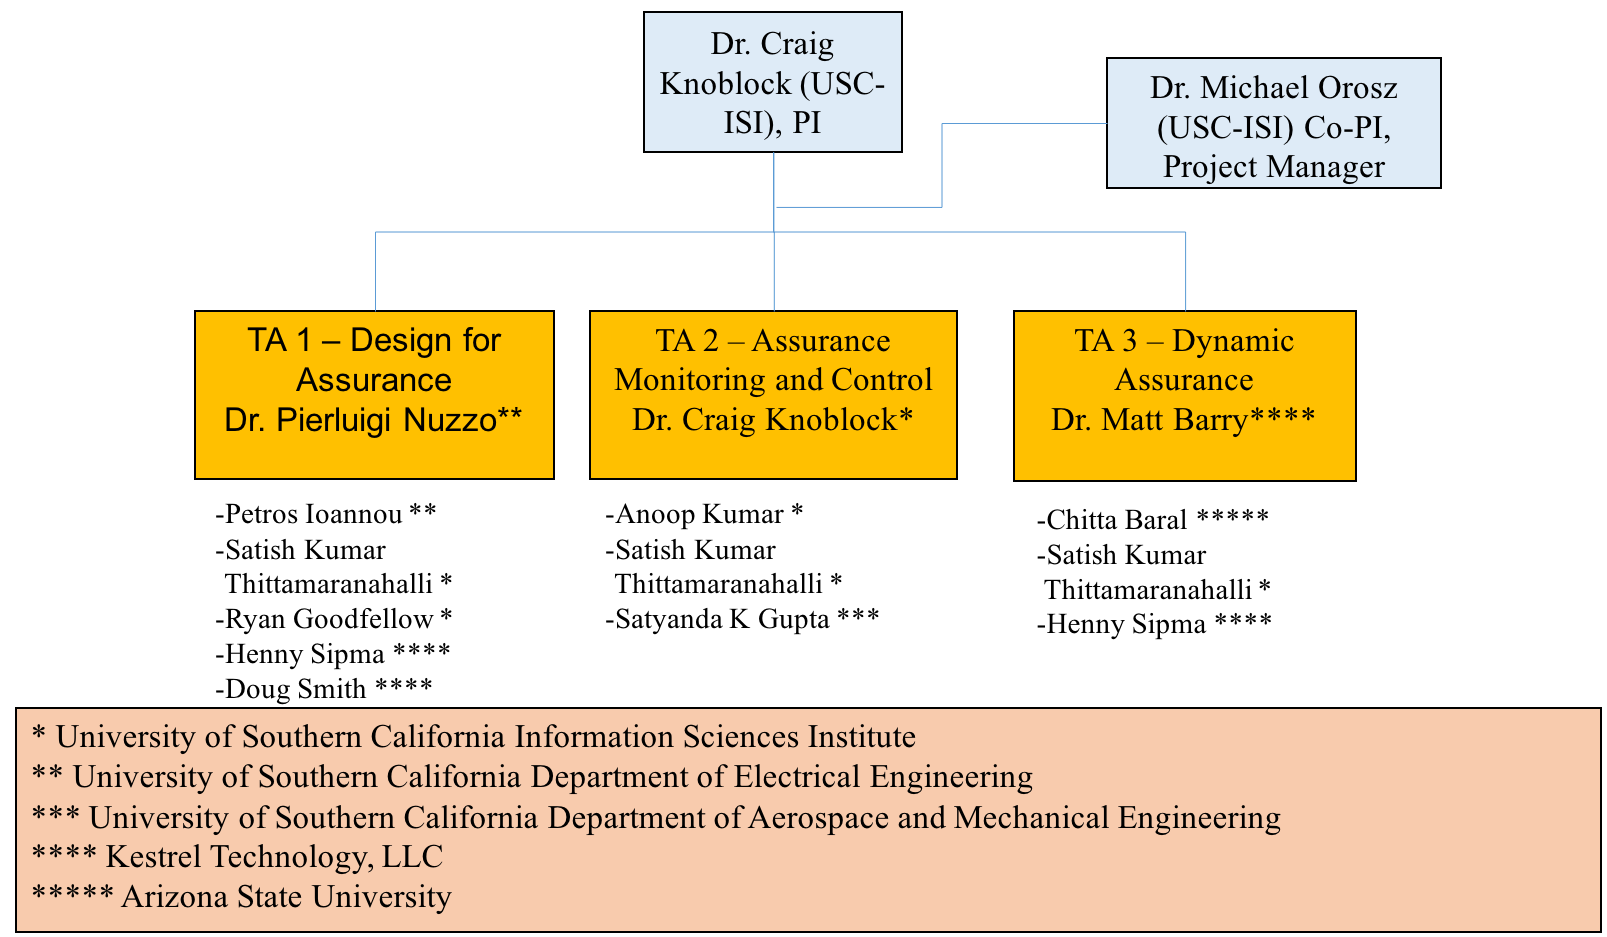
\includegraphics[width=6.0in]{./org-chart2.png}
\caption{\small Organization Chart}
\label{fig:org_chart}
\end{figure}

Coordination: To maximize collaboration and reduce risk to project failure from lack of communication and technical exchange, we plan to employ a wide variety of working styles and communication/coordination so that all can contribute.  At the core of our project will be regularly scheduled meetings bridging the diversely distributed team (Table~\ref{fig:Collaboration_Table}).  These meetings will address project status, identify challenges, implement risk mitigation strategies and participate in technology exchanges and system integration efforts (when appropriate)

\begin{table}[ht]
\caption{\small Project Meetings and Events}
  \centering
  {\footnotesize
\begin{tabular}{|m{3.15in}|m{3in}|} 
\hline
\textbf{Meeting} & \textbf{Frequency} 
\\\hline
Conference calls among investigators (discuss project status, address concerns and project risks) & Weekly
\\
\hline
Technical exchange and coordination meetings using Bluejeans or another videoconference technology & At least twice a month and more frequently as needed
  \\ 
\hline
Face-to-Face meetings (prior to P/I and demonstration meetings) & Every 3 to 6 months and more frequently (especially at the beginning of the project) as needed
 \\\cline{1-2}

\hline
\end{tabular}
}
\label{fig:Collaboration_Table}
\end{table}

\begin{table}[tbhp]
\caption{\small Key Project Team Member Responsibilities}
  \centering
  {\footnotesize
\begin{tabular}{| m{.75in} | m{3.9in}| m{1.5in}|} 
\hline
\textbf{Key Member} & \textbf{Responsibilities} & \textbf{Tasks} 
\\\hline
Dr.\ Craig Knoblock  & Principal Investigator responsible for project, leads TA 2 – Assurance Monitoring and Control.  Will lead the overall project and lead the TA2 team.  Served as the PI on many DARPA projects and has sucessfully led many large teams.    Effort on project:  25\% &
1.1.6, 1.2.2 1.2.3, 1.2.4, 1.3.4, 1.4.1, 
2.1.6, 2.2.2 2.2.3, 2.2.4, 2.3.4, 2.4.1, 
3.1.6, 3.2.2, 3.2.3, 3.2.4, 3.3.4, 3.4.1
\\
\hline
Dr.\ Michael Orosz & Co-Principal Investigator responsible managing the day-to-day operations of the project, assist technical teams as needed, coordinate with TA4 teams.    Has led many large complex multi-disciplined/multi-organizational projects in academic and industry environments.  Effort on project: 50\%
& 1.1.6, 2.1.6, 3.1.6, 1.4.1, 2.4.1, 3.4.1
  \\ 
\hline
Dr.\ Pierluigi Nuzzo 
& 
Co-Principal Investigator.  Leads the TA 1 - Design for Assurance team and conducts research on the formal methods for the design of the TA1 system.  Research experience on methodologies and tools for the design of cyber-physical systems; contracts, interfaces, and compositional methods for embedded system design; the application of automated formal methods and optimization theory to problems in embedded and cyber-physical systems.  Effort on project: 2 months/year (16.6\%)
& 
1.1.1, 2.1.1, 3.1.1 \\
\hline
Dr.\ Matthew Barry
& 
Key personnel.  Leads the TA 3 – Dynamic Assurance.   He will conduct the research on the dynamic assurance case language editors and parsers, the run-time system, and system integrations. Effort on project:  66\%
& 
1.3.2, 2.3.2, 3.3.2\\
\hline
Dr.\ Chitta Baral
& 
Key personnel responsible for learning assurance rules, supporting assurance rules with uncertainty and improving solver speed.  Expertise on ASP solvers, which will be used to reason about the assurance cases. Effort on project: 20\%
& 
1.3.1, 2.3.1, 3.3.1 \\
\hline
Dr.\ Doug Smith 
& 
Key personnel will support formal methods aspects of TA1, and lead the effort on abstract refinement. Expertise in field of automated correct-by-construction program generation.    Effort on project: 40\%
& 
1.1.5, 2.1.5, 3.1.5 \\
\hline
Dr.\ Henny Sipma
& 
Key personnel who will support the program verification tasks under TA1.  Will lead the effort on program verification.   Effort on project:  45\%
& 
1.1.5, 2.1.5, 3.1.5, 1.3.2, 2.3.2, 3.3.2 \\
\hline
Dr.\ Petros Ioannou
& 
Key personnel responsible providing and extending the assurance test bed, which will be available at the start of the project for autonomous vehicles.   Effort on project: 1 month/year (8.3\%)
& 
1.1.2, 2.1.2 (optional), 3.1.2 (optional)
\\
\hline
Dr.\ Satyandra Kumar Gupta
& 
Key Personnel providing autonomous command and control expertise to the TA-2 team.   Will lead the research on safety aware learning on TA2.   Past research on physics-aware decision making to facilitate automation.  Effort on project: 1 month/year (8.3\%)
& 
1.2.1, 2.2.1, 3.2.1 \\
\hline
Dr.\ Anoop Kumar 
& 
Key personnel providing support to the TA 2 project team.  Will lead the research on monitoring \& control and detecting distribution shifts.  Effort on project: 50\%
& 
1.2.1, 1.2.2, 1.2.3, 1.2.4, 2.2.1, 2.2.2, 2.2.3, 2.2.4, 3.2.1, 3.2.2, 3.2.3, 3.2.4\\
\hline
Dr.\ Satish Thittamaranahalli
& 
Key personnel developing scalable algorithms for TA1, TA2, and TA3 project teams.  Has extensive experience on scalable algorithm design, machine learning, and constraint reasoning.  Effort on project: 50\%
& 
1.2.1, 1.2.2, 1.2.3, 1.2.4, 2.2.1, 2.2.2, 2.2.3, 2.2.4, 3.2.1, 3.2.2, 3.2.3, 3.2.4, 1.1.4, 2.1.4, 3.1.4 \\
\hline
Dr.\ Ryan Goodfellow
& 
Key personnel providing support to the TA-1 project. Will lead the research on simulation-based testing.  Has extensive experience on simulation-based testing.  Effort on project:  30\%
& 
1.1.3, 2.1.3, 3.1.3 \\

\cline{1-2}

\hline
\end{tabular}
}
\label{fig:Table_Mgmt}
\end{table}



\newpage
\section{Personnel, Qualifications and Commitment}

{\bf Dr.\ Craig Knoblock}, the PI on this effort, is a Research Professor of both Computer Science and Spatial Sciences at the University of Southern California (USC) and Director of the Intelligent Systems Division at the USC Information Sciences Institute.   He received his Ph.D. from Carnegie Mellon University in computer science. 
%His research focuses on techniques for describing, acquiring, and exploiting the semantics of data.  
In previous projects he has worked on developing  scalable approaches to execution monitoring, accurate detection of sensor failures, and   automatic modeling and reconstruction of sensors.  He has published more than 300 journal articles, book chapters, and conference papers on these topics.  Dr. Knoblock is a Fellow of the Association for the Advancement of Artificial Intelligence (AAAI), a Distinguished Scientist of the Association of Computing Machinery (ACM), a Senior Member of IEEE, past President and Trustee of the International Joint Conference on Artificial Intelligence.
%and winner of the 2014 Robert S. Engelmore Award.  

{\bf Dr.\ Michael Orosz}, a Co-PI on this effort, is a Research Associate Professor of Civil and Environmental Engineering at the University of Southern California (USC) and Research Director of the Decision Systems Group at the USC Information Sciences Institute.  Dr. Orosz has over 30 years’ experience in commercial and government software development, basic and applied research, project management, academic research and has developed and deployed several commercially successful products.  His research interests are in machine learning and decision analytics as applied to intelligence analysis and autonomous command and control such as smart building controls.    Dr. Orosz has extensive experience in managing large complex multi-disciplined/multi-teamed research projects. %funded by DARPA, DHS, DoD, DoE, Industry, NASA, NRO, NSA and ONR.   
He received his Ph.D. in computer science from the University of California, Los Angeles.

{\bf Dr.\ Pierluigi Nuzzo}, a Co-PI on this project, is an Assistant Professor in the Department of Electrical Engineering at the University of Southern California. He received the Ph.D. in Electrical Engineering and Computer Sciences from the University of California at Berkeley. 
%in 2015, and the Laurea degree (MS) in electrical engineering (summa cum laude) from the University of Pisa, Italy, and the Sant'Anna School of Advanced Studies, Pisa, Italy.
%
%He has four years of research experience in analog and mixed signal circuit design as a researcher at IMEC, Leuven, Belgium, and over 10 years experience in design methodologies and tools for mixed-signal integrated circuits and cyber-physical systems, as a researcher at the University of Pisa, IMEC, UC Berkeley, and USC. 
His research interests
include: methodologies and tools for cyber-physical system and mixed-signal
system design; contracts, interfaces and compositional methods for embedded
system design; the application of formal methods and optimization theory to problems in embedded and cyber-physical systems and electronic design automation. 
%
Prof. Nuzzo received %First Place in the operational category and Best Overall
%Submission in the 2006 DAC/ISSCC Design Competition, 
a Marie Curie Fellowship
from the European Union in 2006, 
the University of California at Berkeley EECS
departmental fellowship in 2008, 
%the University of California at Berkeley Outstanding Graduate Student Instructor Award in 2013, 
the IBM Ph.D.
Fellowship in 2012 and 2014, 
%the Best Paper Award from the International Conference on Cyber-Physical Systems (ICCPS) in 2016, 
and the David J.~Sakrison Memorial Prize in 2016 for his doctoral research. 
%He is an author of 1 patent and over 60 publications.

{\bf Dr.\ Satyandra K. Gupta} is Smith International Professor in the Department of Aerospace and Mechanical Engineering at the University of Southern California. %Prior to joining the University of Southern California, he was a Professor in the Department of Mechanical Engineering and the Institute for Systems Research at the University of Maryland. He was the founding director of the Maryland Robotics Center and the Advanced Manufacturing Laboratory at the University of Maryland. 
He served as a program director for the National Robotics Initiative at the National Science Foundation from September 2012 to September 2014.  Dr. Gupta's interest is in the area of physics-aware decision making to facilitate automation. He has published more than 300 technical articles. He is a fellow of the American Society of Mechanical Engineers (ASME) and editor of ASME Journal of Computing and Information Science in Engineering. Dr. Gupta has received the Young Investigator Award from the Office of Naval Research in 2000, CAREER Award from the National Science Foundation in 2001, Presidential Early Career Award for Scientists and Engineers (PECASE) in 2001, Invention of the Year Award at the University of Maryland in 2007, Kos Ishii-Toshiba Award from ASME in 2011, and Excellence in Research Award from ASME in 2013.%, and Distinguished Alumnus Award from Indian Institute of Technology, Roorkee in 2014. %He has also received seven best paper awards at conferences.

{\bf Ryan Goodfellow} is a computer scientist at ISI working in combined cyber physical simulation and emulation platform development. His formal background is in simulation algorithms and modeling techniques using differential-algebraic equations (DAE). He has applied this knowledge in the CPS space by integrating DAE modeling languages and simulation engines with network testbeds to create comprehensive scientific experimentation platforms for cyber-physical systems. These experimentation platforms have been used in the power grid research space. %Ryan is a lead developer on the Deter network testbed, with a strong background in networked and distributed systems engineering. %He is also a combat veteran, serving as a non-commissioned officer and SIGINT team lead for a multi-functional intelligence team in Afghanistan.

{\bf Dr.\ Petros Ioannou} is a Professor in the Department of Electrical Engineering, Director of the Center for Advanced Transportation Technologies and Associate Director for Research for the DOT supported University Transportation Center at USC. He received his MS and PhD from the University of Illinois at Urbana Champaign in Mechanical and Electrical Engineering, respectively. His research interests are in robust adaptive control, vehicle dynamics and control, human factors and safety, automated vehicles, nonlinear systems and Intelligent transportation Systems.  He received the 2016 IEEE Transportation Technologies field award and the 2016 IEEE Control system society Transition to Practice Award. He is a Fellow of IEEE, IFAC and IET and author/coauthor of 8 books and over 400 papers.

{\bf Dr.\ Matthew Barry} will serve as lead for the TA3 tasks. %He will implement the dynamic assurance case language editors and parsers, the run-time system, and system integrations.  He will implement the assurance case arguments and the API for updating argument structure and content.  
Dr. Barry currently is CEO at Kestrel Technology LLC, and previously spent 20 years in NASA space mission operations at the Jet Propulsion Lab and Johnson Space Center.  At NASA Headquarters he led the introduction of dependability case requirements and plans for flight computing systems in upcoming manned space exploration missions, as well as the development of Agency-level software-related safety-critical control system requirements.  He recently served as a Principal Investigator on DHS/Cyber S\&T STAMP (Static Tool Analysis Modernization Program), DARPA CSFV (Crowd Sourced Formal Verification), three NASA Aeronautics R\&D projects, and the AFRL-sponsored Static Analysis of Numerical Algorithms project.  Dr. Barry earned BSME, MS, and PhD degrees in mechanical engineering, and an MBA degree, from Rice University.  

{\bf Dr.\ Henny Sipma} will support the program verification tasks under TA1.  %She is the key person behind the company's {\em KT Advance\/} and {\em KT Transferal\/} static analysis products, and the designer and programmer of the company's core {\em CodeHawk\/} abstract interpretation engine. 
Dr. Sipma currently is the CTO at Kestrel Technology LLC.  She has spent the past 10 years with Kestrel Technology as a static analysis expert; previously developed and taught static analysis techniques as senior research associate at Stanford University for eight years; and developed industrial process controls as an senior systems analyst at Shell.  She has been Principal Investigator or company lead on several recent R\&D projects for Federal agencies, including two projects under the IARPA STONESOUP (Securely Taking On New Executable Software of Uncertain Provenance) program; the DHS Cyber S\&T Gold Standard project; and the DARPA-sponsored STAC (Space-Time Analysis for Cybersecurity) and MUSE (Mining and Understanding Software Enclaves) programs.  Dr. Sipma earned 
%a BS degree in chemistry and an MS degree in chemical engineering at the University of Groningen in The Netherlands, and 
MS and PhD degrees in computer science from Stanford University.  

{\bf Dr.\ Douglas R.\ Smith} will support formal methods aspects of TA1, including the enforcement of safety properties and the generation of monitors.  He is President of Kestrel Technology LLC and Principal Scientist at Kestrel Institute.  He is a Fellow of the American Association of Artificial Intelligence (AAAI) and an ASE Fellow (Automated Software Engineering).  From 1986 to 2000, he taught an advanced graduate course on correct-by-construction software development at Stanford.  
%Dr. Smith has led the development of a series of software synthesis systems, including KIDS (Kestrel Interactive Development System), Specware, Designware, and Planware. 
%Applications domains have included a variety of complex high-performance planners and schedulers for the US Air Force.  He leads current projects on the generation of air mission plans and cyberoperations.  
Other recent projects focused on automated policy enforcement \cite{SmithD0703,SmithD08}, synthesis of secure network protocol codes, and the synthesis of high-performance constraint-solvers\cite{SmithD08c,SmithD13}.  Dr. Smith has over 30 years experience in the field of automated correct-by-construction program generation and has published over 100 papers. He has one patent.  He received the Ph.D. in Computer Science from Duke University% in 1979.  

{\bf Dr. Chitta Baral} is a Professor in the Department of Computer Science and Engineering at Arizona State University. He will support the TA3 efforts on Learning assurance rules, supporting assurance rules with uncertainty and improving solver speed. Dr. Baral has expertise in various aspects of autonomy and Artificial Intelligence. 
He wrote the first book on answer set programming (published by Cambridge University Press) the formal language behind our assurance rules. Some of his other works relevant to this proposal are: goal specification for autonomous systems, automatic construction of control rules for autonomous systems that satisfy given goals, combining machine learning with reasoning in various contexts, including image understanding. %He is the President of KR Inc. He is an associate editor of AIJ and has been an associate editor of JAIR.

{\bf Dr.\ Satish Kumar Thittamaranahalli (T. K. Satish Kumar)} leads the Collaboratory for Algorithmic Techniques and Artificial Intelligence (CATAI) at USC's Information Sciences Institute. He has published over 60 papers on numerous topics in Artificial Intelligence spanning such diverse areas as Constraint Reasoning, Planning and Scheduling, Probabilistic Reasoning, Robotics, Combinatorial Optimization, Approximation and Randomization, Heuristic Search, Model-Based Reasoning, Knowledge Representation and Spatio-Temporal Reasoning. %He %has served on the Program Committees of many international conferences in Artificial Intelligence
He and is a winner of the 2016 Best Robotics Paper Award and the 2005 Best Student Paper Award from the International Conference on Automated Planning and Scheduling. 
Dr. Kumar received his PhD in Computer Science from Stanford University. %In the past, he has also been a Visiting Student at the NASA Ames Research Center, a Postdoctoral Research Scholar at the University of California, Berkeley, a Research Scientist at the Institute for Human and Machine Cognition, a Visiting Assistant Professor at the University of West Florida, and a Senior Research and Development Scientist at Mission Critical Technologies.

\textbf{Dr.\ Anoop Kumar} is a senior computer scientist at USC ISI and has broad expertise in machine learning, statistical modeling, and software engineering.  Dr.\ Kumar is the technical lead on the DARPA RSPACE program and has played a vital role in developing a system that fuses air operations data from multiple sources, maintains world state, and issues warnings. Previously, he led the research and development of the BBN’s election forecasting system for the IARPA OSI program. %Dr.\ Kumar played a significant role in the DARPA DEFT program by developing a model to support integration of output from multiple NLP algorithms. He has contributed at the development to management levels on government research contracts and commercial projects. 
Dr.\ Kumar helped design and develop BBN's commercially available, hosted speech and medical transcription services offering. 

\begin{table}[!tbh]
\begin{footnotesize}
\vspace{-0.1in}

\begin{tabular}{lll}
\begin{tabular}[t]{|l|@{}c@{}|@{}c@{}|@{}c@{}|@{}c@{}|} \hline
Project & Status & \multicolumn{3}{ c| }{Hours} \\ \cline{3-5}
& & P1 & P2 & P3 \\ \hline



\multicolumn{5}{ |c| }{ \textbf{Craig Knoblock} } \\ \cline{1-5}
Safeguard & Pro & 770 & 641 & 641 \\ \cline{1-5}
ELICIT & Cur & 308 & 256 & 120 \\ \cline{1-5}
WTNIC & Cur & 11 & 0 & 0 \\ \cline{1-5}
EFFECT & Cur & 641 & 107 & 0 \\ \cline{1-5}
LinkedMaps & Cur & 203 & 25 & 0 \\ \cline{1-5}
PRINCESS & Cur & 608 & 96 & 0 \\ \cline{1-5}
SCHARP & Cur & 481 & 54 & 0 \\ \cline{1-5}
MINT & Pen & 650 & 534 & 285 \\ \cline{1-5}

\multicolumn{5}{ |c| }{ \textbf{Michael Orosz} } \\ \cline{1-5}
Safeguard & Pro & 1560 & 1300 & 1300  \\ \cline{1-5}
SMC/SY & Cur & 1803 & 0 & 0  \\ \cline{1-5}

\multicolumn{5}{ |c| }{ \textbf{Matthew Barry} } \\ \cline{1-5}
Safeguard & Pro & 2078 & 1690 & 1554 \\ \cline{1-5}
Starlite & Cur & 1840 & 1692 & 0 \\ \cline{1-5}



\multicolumn{5}{ |c| }{ \textbf{Anoop Kumar} } \\ \cline{1-5}
Safeguard & Pro & 1560 & 1300 & 1300 \\ \cline{1-5}

\end{tabular}
&
\begin{tabular}[t]{|l|@{}c@{}|@{}c@{}|@{}c@{}|@{}c@{}|} \hline
Project & Status & \multicolumn{3}{ c| }{Hours} \\ \cline{3-5}
& & P1 & P2 & P3 \\ \hline

\multicolumn{5}{ |c| }{ \textbf{Pierluigi Nuzzo} } \\ \cline{1-5}
Safeguard & Pro & 520 & 433 & 433  \\ \cline{1-5}
Mirage & Cur & 433 & 0 & 0  \\ \cline{1-5}

\multicolumn{5}{ |c| }{ \textbf{Satyandra Gupta} } \\ \cline{1-5}
Safeguard & Pro & 260 & 217 & 217 \\ \cline{1-5}
Human   & Cur & 22 & 0 & 0 \\ \cline{1-5}
Vehicles & Cur & 36 & 0 & 0 \\ \cline{1-5}
Robot & Cur & 116 & 0 & 0 \\ \cline{1-5}
Assembly & Cur & 33 & 0 & 0 \\ \cline{1-5}
Solar & Cur & 4 & 0 & 0 \\ \cline{1-5}

\multicolumn{5}{ |c| }{ \textbf{Petros Ioannou} } \\ \cline{1-5}
Safeguard & Pro & 260 & 217 & 217 \\ \cline{1-5}
CPS & Cur & 130 & 0 & 0 \\ \cline{1-5}

\multicolumn{5}{ |c| }{ \textbf{Ryan Goodfellow} } \\ \cline{1-5}
Safeguard & Pro & 936 & 780 & 780 \\ \cline{1-5}
STEAM & Cur & 416 & 0 & 0 \\ \cline{1-5}


\end{tabular}
&
\begin{tabular}[t]{|l|@{}c@{}|@{}c@{}|@{}c@{}|@{}c@{}|} \hline
Project & Status & \multicolumn{3}{ c| }{Hours} \\ \cline{3-5}
& & P1 & P2 & P3 \\ \hline

\multicolumn{5}{ |c| }{ \textbf{Chitta Baral} } \\ \cline{1-5}
Safeguard & Pro & 659 & 485 & 485 \\ \cline{1-5}
PostdocBP & Cur & 176 & 0 & 0 \\ \cline{1-5}
Languages & Pen & 528 & 264 & 264 \\ \cline{1-5}
CAREER & Pen & 88 & 44 & 44 \\ \cline{1-5}
CHS & Pen & 510 & 255 & 0 \\ \cline{1-5}

\multicolumn{5}{ |c| }{ \textbf{Doug Smith} } \\ \cline{1-5}
Safeguard & Pro & 1222 & 984 & 840 \\ \cline{1-5}
RSPACE & Cur & 342 & 0 & 0 \\ 
\cline{1-5}
PLANX & Cur & 154 & 0 & 0 \\ 
\cline{1-5}
HACCS & Pen & 923 & 769 & 769 \\ 
\cline{1-5}

\multicolumn{5}{ |c| }{ \textbf{Henny Sipma} } \\ \cline{1-5}
Safeguard & Pro & 1372 & 962 & 840 \\ \cline{1-5}
STAC & Cur & 797 & 0 & 0 \\ \cline{1-5}

\multicolumn{5}{ |c| }{ \textbf{Satish Thittamaranahalli} } \\ \cline{1-5}
Safeguard & Pro & 1560 & 1300 & 1300 \\ \cline{1-5}
MapF & Cur & 103 & 103 & 0 \\ \cline{1-5}

\end{tabular}
\end{tabular}

\end{footnotesize}
\caption{Individual commitments of key personnel}
\label{tab:Commitments}
\vspace{-0.2in}
\end{table}

\clearpage
\newpage
\section{Capabilities}


%\subsection{University of Southern California}
USC has strengths in number of areas that are closely related to the proposed work:
\begin{itemize}[itemsep=0pt,leftmargin=*]
\item Dr.\ Nuzzo 
%has over 10-year research experience in embedded system design, from mixed-signal chip design (analog-to-digital converters, frequency synthesizers, software-defined radio), to methodologies and tools for mixed-signal integrated circuits and Cyber-Physical Systems (CPSs), and the application of formal methods and optimization theory to problems in embedded and cyber-physical systems and electronic design automation.  
%His doctoral work 
has done extensive research on contracts and compositional methods for heterogeneous system design and design space exploration, with application to aircraft electric power systems and environmental control systems. His work has helped transition rigorous system design foundations, innovative design methodologies, and new systems engineering paradigms to industry (IBM, United Technologies). 
\item Dr.\ Satyandra K. Gupta has worked on autonomous surface vehicles, autonomous ground vehicles for operation on rugged terrains, and autonomous flapping wing aerial vehicles.   His group has developed a hierarchal decision making approach for realizing autonomous systems. 
%This approach combines task planning and assignment, deliberative trajectory planning, reactive collision avoidance behaviors, and trajectory tracking control layers. 
His group has also developed new methods for learning reactive behaviors in adversarial environments and COLREGS compliant trajectory planning. \item Dr.\ Knoblock has developed methods that learn the relationships between sensors to both identify failures and changes in sensor and reconstruct those sensors, providing estimates of the accuracy of the reconstructed sensors.  
\item Ryan Goodfellow has extensive experience in simulation based testing through high-fidelity CPS testbed environment development and operation, using the Deter network testbed as the core which has supported several large scale government projects from a variety of agencies and thousands of users. %we have developed sophisticated CPS experiments under programs such as NFS RIPS, NIST SmartCities and the DHS Cybersecurity showcase.
\item Dr.\ Ioannou %helped  design and implement adaptive cruise control systems in collaboration with Ford Motor Company, which was commercialized four years before any other company. He 
worked on several DOT funded projects on automated vehicles and intelligent highway systems where he demonstrated his vehicle control designs for safety and performance on actual automated vehicles in test trucks and I-15 highway.
\item Drs.\ Knoblock, Kumar, and Thittamaranahalli have developed highly scalable approaches for monitoring message traffic to identify potential problems and issue warnings and alerts. 
\item Dr. Thittamaranahalli has developed state-of-the-art methods for efficiently solving large-scale search and optimization problems. %These techniques will be applicable in TA2 for safety-aware learning and planning, in TA2 for assurance monitoring and control, and in TA3 for dynamic assessment of assurance cases.

\end{itemize}
%\subsection{Kestrel Technology LLC}

Kestrel Technology's strength is in program analysis, specifically static analysis of both source and binary targets.  The company performs applied R\&D and product development for a variety of static analysis applications  pivoting primarily on the abstract interpretation technique.  The company recently initiated development of program analysis applications using logical equivalence techniques. As a provider of verification evidence in the form of mathematical proofs, the company also has expertise in the design and development of assurance case arguments for high-integrity systems using such evidence. %The company is engaged in a partnership with Wind River Systems to develop program analysis tools for its embedded system developers.  Many of Wind River's customers must develop their products under safety and certification standards, including those using safety cases.  

   

%\subsection{Arizona State University}
Chitta Baral at Arizona State University has developed various software to learn assurance rules and various ASP solvers, which he has made available as open-source.

Most of the software carried forward for implementation or derivation is open source.  The single exception is Kestrel Technology's {\it KT Advance\/} static analysis tool (TA1), in particular the abstract interpretation engine therein, which is company proprietary and is US EAR export-controlled.   
%Owing to mixed funding for the development of that technology 
We will continue to provide the Federal government a restricted use license for that particular item.

There are no specialized facilities, data, or GFE required for this effort. 

\include{sow}
\include{milestones}

% \section{Level of Effort by Task \textcolor{red}{[Mike/Lisa - 1 pages]}}

% \textcolor{blue}{
% \begin{itemize}
% \item Will be a separate spreadsheet
% \item
% \end{itemize}
% }

\include{appendix_a}

%\section{Appendix B \textcolor{red}{[No Page Count]}}

\section{References}
\bibliographystyle{acm} 
\bibliography{TA3/ta3,TA2/ta2,TA1/ta1}
\end{document}
%%\documentclass[a4paper]{article}
%\documentclass[12pt]{article}
\documentclass[12pt]{dod-blank}

%% Language and font encodings
\usepackage[english]{babel}
\usepackage[utf8x]{inputenc}
\usepackage[T1]{fontenc}

%% Sets page size and margins
%%\usepackage[a4paper,top=3cm,bottom=2cm,left=3cm,right=3cm,marginparwidth=1.75cm]{geometry}
%\usepackage[top=1in, bottom=1in, left=1in, right=1in]{geometry}



%% Useful packages
\usepackage{amsmath}
\usepackage{graphicx}
  \graphicspath{{.}{./image/}}
  \DeclareGraphicsExtensions{.png,.jpg} 
\usepackage[colorinlistoftodos]{todonotes}
\usepackage[colorlinks=true, allcolors=blue]{hyperref}
\usepackage{tabularx}
\usepackage{multirow}
\usepackage{tabulary}
\usepackage{float}
\usepackage{wrapfig}
\usepackage[export]{adjustbox}
\usepackage{comment}
\usepackage{tabularx}
\usepackage{multirow}
\usepackage{tabulary}
\usepackage{enumitem}

\usepackage{listings}
\usepackage{color}
\usepackage{array}
\usepackage{subcaption}
\usepackage{xcolor}




\renewcommand{\textfraction}{0}
\renewcommand{\topfraction}{1.0}
\renewcommand{\bottomfraction}{1.0}

\usepackage{longtable}
%% macros
\newif\iffinal
\finaltrue
\iffinal
  
    \newcommand\baareq[1]{}
    \newcommand\baades[1]{}
 
 
\else
    \definecolor{darkgreen}{rgb}{0,0.4,0}
    \definecolor{darkcyan}{rgb}{0,0.4,0.4}
    \definecolor{darkblue}{rgb}{0,0,0.5}
    
    \newcommand\baareq[1]{{\color{darkcyan}[\textbf{Requirement:} #1]}}
    \newcommand\baades[1]{{\color{darkcyan}[\textbf{Description:} #1]}}
 
\fi




\def\naive{na\"{\i}ve}



\lstset{ 
  backgroundcolor=\color{white},   % choose the background color; you must add \usepackage{color} or \usepackage{xcolor}
  basicstyle=\footnotesize\ttfamily,            % the size of the fonts that are used for the code
  breakatwhitespace=false,         % sets if automatic breaks should only happen at whitespace
  breaklines=true,                 % sets automatic line breaking
  captionpos=b,                    % sets the caption-position to bottom
  commentstyle=\color{mygreen},    % comment style
  % deletekeywords={...},            % if you want to delete keywords from the given language
  escapeinside={\%*}{*)},          % if you want to add LaTeX within your code
  extendedchars=true,              % lets you use non-ASCII characters; for 8-bits encodings only, does not work with UTF-8
  frame=single,	                   % adds a frame around the code
  keepspaces=false,                 % keeps spaces in text, useful for keeping indentation of code (possibly needs columns=flexible)
  keywordstyle=\color{blue}\bfseries\underbar,       % keyword style
  language=Prolog,                 % the language of the code
  % morekeywords={if,and},        % if you want to add more keywords to the set
  numbers=none,                    % where to put the line-numbers; possible values are (none, left, right)
  numbersep=5pt,                   % how far the line-numbers are from the code
  numberstyle=\tiny\color{mygray}, % the style that is used for the line-numbers
  rulecolor=\color{black},         % if not set, the frame-color may be changed on line-breaks within not-black text
  showspaces=false,                % show spaces everywhere adding particular underscores; it overrides 'showstringspaces'
  showstringspaces=false,          % underline spaces within strings only
  showtabs=false,                  % show tabs within strings adding particular underscores
  stepnumber=2,                    % the step between two line-numbers. If it's 1, each line will be numbered
  stringstyle=\color{mymauve},     % string literal style
  tabsize=2,	                   % sets default tabsize to 2 spaces
  title=\lstname                   % show the filename of files included with \lstinputlisting; also try caption instead of title
}

% apply trick for additional keywords for our AC DSL
\lstset{
	emph={for, if, and, or},
    emphstyle={\color{blue}\bfseries\underbar}
}




\title{DARPA Assured Autonomy}
\author{Technical Volume- \textcolor{red}{Thirty-Eight (38) pages max}}

\begin{document}
\pagenumbering{roman}
\include{cover}

\newpage
\section{Table of Contents}
\tableofcontents

\newpage
\pagenumbering{arabic}
\section{Executive Summary}
As we rapidly move into a world where machine learning plays a central role in realizing autonomous systems, it is becoming increasingly important to develop techniques that assure that these systems will operate safely and perform as expected. Current approaches are limited to providing assurance for systems with limited or no  learning capabilities. In this context, DARPA's Assured Autonomy BAA seeks to \emph{develop rigorous design and analysis technologies for continual assurance of learning-enabled autonomous systems}. USC in collaboration with Kestrel Technology and ASU is pleased to submit a comprehensive TA1, TA2, and TA3 proposal entitled \emph{``Assured Autonomy for Learning Enabled Vehicles (Safeguard).''} We plan to provide an end-to-end solution to support autonomous systems with learning-enabled components, ranging from design technologies for assurance, to assurance monitoring and control techniques, to representation and online evaluation of assurance cases. We have assembled a strong team of experts that cover the range of technologies that are required to create such an end-to-end system. If successful, the project will provide the technologies for building the next-generation of learning-enabled autonomous systems.  The entire project will take four years and cost \textcolor{red}{\$??}, with an initial version completed at the end of Phase I and successive versions with additional capabilities and improved scalability at the end of Phase II and Phase III.  

In the remainder of this section, we first introduce an  unmanned surface vehicle scenario that will be used throughout the proposal to describe the approach.  Next, we describe our approach to design, monitoring, and dynamic assurance. Finally, we introduce the team involved in the project. 

\textbf{Motivating Scenario.} Consider an autonomous unmanned surface vehicle (USV) guarding a valuable asset in the ocean when an unknown vehicle  approaches the security perimeter, under challenging weather conditions. In this scenario, the USV is required to approach the intruding vehicle, issue a warning signal, and escort it to a safe distance from the controlled area. However, as the USV has no a priori knowledge of its external environment behaviors (e.g., water depth, waves, wind, current, visibility), pre-computing a feasible trajectory, let alone optimal, becomes a non-trivial problem. For trajectory planning, the USV must continuously perform the following tasks:
\begin{itemize}[itemsep=0pt,leftmargin=*]
 \item Sense the current state of the surrounding environment (e.g., water depth, waves, wind, current, visibility) and estimate its own maneuverability constraints (e.g., braking distance, available acceleration, maximum velocity, turning radius, turning rate, safety distance) based on the state of the environment;      
\item Sense the static obstacles in the sensor range and generate a traversability map;
\item Sense the moving obstacles and classify them;   
\item Predict future trajectories of moving obstacles; 
\item Determine if any of the COLREGS \cite{commandant1999international} rules will be in effect with respect to one or more of the nearby vessels and identify the vessels with the right of way.    
\end{itemize}
The above information will be used by the trajectory planner to compute an initial trajectory, which will be continuously refined as the USV gathers additional information.
% It is not possible for the USV to be tested in every possible environment. 
The USV will use learning enabled components to take  decisions as it encounters new situations, such as  
\begin{itemize}[itemsep=0pt,leftmargin=*]
\item Classifiers to identify moving obstacles based on physical appearance and motion signatures,
\item Algorithms to estimate the sensor capabilities in adverse weather conditions,   
\item Algorithms to accurately estimate uncertainty in the environment, 
\item Classifiers to generate traversability maps,
\item Prediction of external vessel behaviors based on motion histories, 
\item Reinforcement learning  to ensure COLREGS compliance of maneuvers,  
\item Algorithms to learning pursuit behaviors.  
\end{itemize}
Learning enabled components will interact with each other in complex ways, where a misclassification error in one component may eventually compromise the entire mission.   
% We will need to make sure that each learning enabled components has a run-time monitor that will ensure that the assumptions made by the learning-enabled component remain valid and prevent erroneous learning. 
% For example, if the vehicle is exhibiting significant error in trajectory tracking, then simply downgrading the trajectory tracking error value may not be a good option.  The failure of prediction of trajectory tracking error might be due to the presence of a significant wake caused by a nearby vessel. The presence of the nearby vessel can be used to explain the degradation in trajectory tracking performance. As the vessel moves away, we can expect the trajectory tracking performance to return to the predicted level.  
While exhaustive validation of learning-enabled cyber-physical systems (LE-CPSs) is a prohibitive task~\cite{Kalra16},
their complexity, heterogeneity, and highly dynamic nature
make it challenging to even leverage existing model-based development techniques to effectively assess system correctness 
% dependability, 
at design time or enforce it at runtime.

\textbf{Design for Assurance.} Safeguard uses a platform-based design approach~\cite{Nuzzo15b} to organize the design process for a LE-CPS and to build assurance cases. Composite models are developed at several levels of abstraction,
from top-level system requirements and safety constraints down to the
implementation level.  Intermediate levels add detail to the levels
above.  The different levels are connected by refinement mappings that
allow properties established at one level to be preserved at the next
level (see Figures~\ref{fig:methodology} and~\ref{fig:assurance}).

Contracts are used to formally specify components and composite models
in terms of (1) Assumptions -- the assumed behaviors of the
environment and the behaviors of other components, and (2) Guarantees
-- the behavior properties that a model guarantees if it operates in a
context that satisfies its assumptions.  A calculus of contracts
allows horizontal composition of contracts to generate contracts for
composite models.  Vertical contracts are used to specify the mapping
or refinement relation between models at different levels of
abstraction.  The system design process starts with a high-level
contract that expresses overall system assumptions and requirements.
Subsequent levels express models with increasing detail until the
lowest level expresses the system in terms of hardware components and
their software controllers.

The assurance case for a CPS arises from the horizontal and vertical
structure of the design in several ways.  The components used within a
particular level are either (1) synthesized using
correct-by-construction design tools together with proofs, (2) derived
statically or dynamically using safety-aware machine-learning
techniques, (3) written manually and verified by analysis tools, or
(4) written manually and validated by extensive testing.  The
assurance case for the whole reflects its compositional structure.  We
anticipate that well-specified contracts together with the calculus of
contracts will eliminate well-known problems with unexpected emergent
behaviors in CPS systems.

The assurance case for the lowest-layer design arises from both the
intra-level assurance and from properties and their proofs that are
preserved under the refinement mapping from the top-level
requirements.  The refinement mappings between model layers will be
constructed using a variety of techniques.  A contract at an abstract
level can be mapped to a component or refined contract by (1)
retrieval of pre-verified components from a platform library, (2)
synthesis using correct-by-construction design and optimization tools,
or (3) manual coding to satisfy a contract.  The mapping of a
composite model will be composed from the mappings of its constituent
components or contracts.  When a composite model cannot be mapped
compositionally to the next level, it will be generated using
correct-by-construction design and optimization tools.

\textbf{Assurance Monitoring and Control.}
We provide an integrated framework for safety-aware learning, assurance monitoring and control, detecting distribution shifts. Three major components offer an efficient TA2 architecture as well as interfaces with TA1 and TA3, that is, (a) safety-aware learning and planning, (b) assurance monitors for guarding architectural and safety constraints; and (c) distribution shift detection.

We will develop a new learning-enabled online decision-making framework that allows opportunistically composing a sequence of actions (maneuvers) to reduce uncertainty in the system capability model without suspending the progress toward the mission goals or compromising safety. Each candidate action is evaluated based on three criteria: (1) the risk of violating a safety constraint using the current uncertainties in the parameter estimates; (2) its relevance to the mission goals; (3)  its expected information gain, i.e., reduction in uncertainty, with respect to the parameter estimates. These evaluations are combined to produce a cumulative mission utility value for each action that drives our learning-enabled decision-making framework. The problem of generating and evaluating sequences of actions can be posed in several way. For example, it can be solved using a branch-and-bound search method like Anytime A*, or formulated with the finite-horizon Markov Decision Process (MDP) framework. We will develop new scalable search strategies to solve this problem efficiently, by potentially evaluating a recent method developed at USC, called FastMap, that can significantly improve the execution time. 

We will develop monitors for architectural and safety constraints. 
% While these constraints can be checked over and over again as sensor information flow in, this naive strategy accounts for a lot of computational overhead. 
To achieve scalability and decrease the overhead, we propose the application of a technique that we currently use in DARPA's RSPACE program, which leverages a physical model of the vehicles dynamics and its interactions with the environment to efficiently determine the readout frequency. We propose two  extensions of this basic idea. First, we will use the theory of Variable Elimination to prioritize which variables to monitor, e.g., controllable, versus uncontrollable, adversarially controlled, or unobservable variables. Second, we invoke the dynamic assessment of assurance cases only when needed. This  decreases the number of times dynamic assessment of assurance cases is initiated as well as the communication bandwidth between the TA2 and TA3 components.

Finally, we will identify a distribution shift by combining statistical and machine learning techniques to differentiate between environmental and sensor changes. We will exploit a categorization of the shifts based on their cause and duration as well as extend our earlier work on detecting and mitigating sensor failures for all types of monitored variables.  

\textbf{Dynamic Assurance:} The Safeguard {\em design for assurance\/} activity takes a systems-theoretic stance toward safety.  Consequently, it presumes that safety is an emergent property of the system, and that hazards can present themselves through unintended interactions and performance violations in addition to causal events such as component failures.  Our design approach includes consideration of intent as well as hazard analysis and mitigation.  The artifacts from these activities populate contracts and assumptions for the dynamic assurance case.  
We thus build safety into the product by working at a systems-level viewpoint, using lexicon and design patterns familiar to both hardware and software engineers; safety is an emergent property of the system, not an afterthought.  
As system behavior evolves during runtime owing to learning, threats, degradation, or some other factor, the dynamic assurance case identifies whether the safety constraints continue to be satisfied.  If not, it provides notifications or issues recovery instructions directly from a lookup table.

Our implementation of the dynamic assurance case employs a declarative knowledge base inference engine and a domain-specific language tailored to our approach.  We have used them successfully for assurance case tool sets and arguments, and will extend them to reason about uncertainty and learning.  Our approach to achieve scalability is to specialize solvers toward modularity and to take advantage of domain knowledge.  Specifically, we will develop answer set programming techniques for context-dependent learning for reasoning about the learning-enabled components as well as learning assurance rules.  We will develop new formalisms for uncertainty to include causality, using weights for computing probabilities, and probabilistic non-monotonicity.  To achieve scaling objectives we will implement specializations using modularity, weighted CSPs, and message passing. 

% The system safety constraints revealed from that design become the key elements of our dynamic assurance case.  Our verification tools ensure the constraints are relevant, identifiable, and their implementation and effect observable.  

\textbf{Team.} We have assembled a team that is exceptionally well-qualified to build the proposed Safeguard system.  The team will be led by Dr.\ Craig Knoblock, the Principal Investigator for the effort, who currently leads the Intelligent Systems Division at the Information Sciences Institute.  He has led many large DARPA and IARPA projects over the years and has a strong track record in conducting leading edge research and then transitioning the technology to commercial use.  He will be supported by Dr.\ Michael Orosz as the Project Manager, who also has  experience in managing large research projects and on autonomous systems.  The TA1 team will be led by Dr.\ Pierluigi Nuzzo, who is an expert in embedded system design methodologies and the  application of formal methods to cyber-physical systems.  The TA1 team also includes Dr.\ Doug Smith, who has spent many years working on scalable correct-by-construction techniques and Dr.\ Henny Sipma, who has significant experience in applying program verification methods to real-world problems.  The TA1 team also includes Ryan Goodfellow, who has done a large amount of work on simulation-based testing.  The TA2 team will be led by Dr.\ Knoblock who has worked on topics related to both monitoring and detecting distribution changes.  He will be supported by Dr.\ Satyandra Gupta, who is an expert on autonomous surface vehicles as well as on safety-aware learning. He will also be supported by Drs.\ Anoop Kumar and Satish Thittamaranahalli, who have also previously worked on efficient methods for execution monitoring.  The TA3 team will be lead by Dr.\ Matthew Barry, who has experience in creating the technologies for assurance cases.  He will be supported by Dr.\ Chitta Baral, who is an expert on ASP solvers and by Dr.\ Thittamaranahalli who is an expert on SAT solvers, both of which will be applied to provide scalable assurance case reasoning.  Finally, Dr.\ Petros Ioannou, who is an expert on control systems for autonomous vehicles will provide an autonomous vehicle platform, which will form the focus of our work until the TA4 teams provide additional vehicle platforms for development.  

\newpage
\section{Innovative Claims and Deliverables}

In this project we will develop and build an end-to-end system for assured autonomy.  This section describes the key innovations by technical area and then the overall deliverables of the project.

\paragraph{Design for Assurance}

\begin{itemize}[itemsep=0pt,leftmargin=*]
\item We address the LE-CPS design challenges via a holistic approach that can contextually generate design artifacts and assurance cases. We develop a compositional, contract-based modeling framework, methods, and tools to support the design process from system-level requirement capture,  formalization, and analysis, to the generation, testing, and continual monitoring of software and hardware artifacts in feedback loop with a physical process.

\item We develop compositional abstractions and interfaces (vertical contracts) that can  bridge heterogeneous formalisms and heterogeneous decomposition architectures to make system analysis and synthesis tractable, consistently combine different verification and synthesis methods at design time, and provide seamless support for dynamic assurance at run time. %We aim to quantitatively capture the confidence in the satisfaction of requirements under uncertain or unknown conditions, and resilience properties of  systems at different abstraction levels, to enable trade-off evaluation between resilience, performance, and cost.

\item We develop a unifying framework and efficient algorithms to reason about the combination of discrete and continuous dynamics and constraints in the presence of uncertainties in LE-CPS using a satisfiability modulo convex approach~\cite{Shoukry2017} for contract-based system verification and scalable trajectory planning.  

\item We provide an environment for high-fidelity CPS testing, in which production-ready software, e.g.,  safety-critical learning and control, may be deployed and tested 
% by extending the Cypress testbed environment \cite{Goodfellow2015Cypress:Systems} 
with time dilation facilities, so that it synchronizes with a physical simulation that is not necessarily running in real time, while still having the perception of real time.

\item We 
% These facilities allow a cyber system to be  
propose an approach for unanticipated behavior space identification and test coverage maximization which leverages results from the theory of differential algebraic equation (DAE)~\cite{Berger2013ControllabilitySurvey,Ilchmann2005ATheory,BergerOnSystems,Lamour2013} 
to prune the behavior search space and identify smaller regions of interest for efficient simulation-based testing. 
% We then compute the intersection of these two behavior spaces and restrict our simulation based testing search space to this subspace.
\end{itemize}

\paragraph{Assurance Monitoring and Control}

\begin{itemize}[itemsep=0pt,leftmargin=*]
\item 
%We integrate safety-aware learning into the overall decision making problem. The goal is to maximize mission utility without violating the safety constraints. 
Our safety-aware learning framework enables the system to opportunistically select and execute actions to assist the learning-enabled component in reducing model uncertainty without compromising safety or deviating from the mission goals. The value of uncertainty reduction is explicitly incorporated in the optimization process for selecting the best action.  
\item For safety-aware learning, we propose the idea of preprocessing the search space of the problem domain before queries and observations come in. With such a linear-time preprocessing phase, the performance of search and optimization algorithms can be significantly boosted. For example, in regular A* search, the intensional or extensional search space can be preprocessed in near-linear time to yield an embedding of each state as a point in Euclidean space~\cite{cujakk}. Then, when the query comes in, A* search can make use of these Euclidean distances as heuristic distances between two states to yield order-of-magnitude speedups. 
%In Anytime A* for safety-aware learning and planning, this leads to a significantly better quality of actions chosen within a time limit, and in the MDP framework, the same ideas can be used to improve the convergence of Bellman updates for safety-aware Reinforcement Learning.
\item As massive amounts of sensor information flow in, it is imperative for us to efficiently process this information for monitoring architectural and safety constraints. Building on our past work on similar tasks, we propose novel technologies for efficiently monitoring constraints. These algorithms can yield an exponential reduction in the amount of sensor data that needs to be processed. Doing this also reduces the message complexities between the various modules. %We also propose to use the theory of Variable Elimination (VE) to monitor constraints with uncontrollable, adversarially controlled, and/or unobservable variables. VE yields a substrate constraint to monitor that characterizes a dominant strategy of the controllable variables over the uncontrollable, adversarially controlled, and/or unobservable variables.
\item We will develop techniques to identify  distributional shifts and determine the underlying cause (e.g., change in environment, sensor failure,   etc.), as well as strategies for handling the various distributional shifts.   Notably, we propose to build on our past work and use compact representations to exploit historical data to identify distributional shifts.
\end{itemize}

\paragraph{Dynamic Assurance}

\begin{itemize}[itemsep=0pt,leftmargin=*]

\item We demonstrate the integration of dynamic assurance for safety-critical learning-enabled dynamic systems in which evolutionary behaviors are expected and tolerated as a property of the functionality.   The impact will be consequential contributions safety-critical dynamic systems in which evolutionary behaviors are expected and tolerated as portion of the functionality.   
\item We implement dynamic assurance by combining features of system safety, formal methods, logic programming, uncertain reasoning, and domain-specific languages.  We populate assurance case arguments at several levels of modeling and implementation abstraction, using the analysis results to produce design-time evidence supporting assurance claims.  
%We provide automated reasoning about the assurance case itself to produce verification, consistency, and completeness results for the argument.  Dynamic assurance results then yield trusted explanations of whether safety constraints and assumptions and other contracts still hold during the collection of runtime evidence from monitors. 
\item We develop and demonstrate ASP formalisms crucial to applications in dynamic assurance. We demonstrate the suitability of the technology especially for assurance case arguments owing to the improved legibility, consistency and completeness checks, handling of uncertain and default reasoning, and scalability.  
%We will produce modularized solvers for enhanced performance based on recent algorithmic developments in exploiting structure, kernelization, and message passing. We provide a formalism to enable learning of assurance rules. 
We provide a novel approach to handling uncertainty that provides the ability to do causal and counter-factual reasoning as well as probabilistic non-monotonicity.  Overcoming limitations of traditional inductive logic techniques, we develop a novel iterative and incremental approach based on context dependent learning. 
\end{itemize}

\paragraph{Deliverables}
During the course of this project, we will build and deliver a fully-operational system that covers all three of the technical areas.  The detailed capabilities of this system are described in the individual technical sections.  The resulting system will be available as open source under a permissive license, which will allow other organizations to use the work, extend it in new directions, and even commercialize the software.  Kestrel Technology has significant experience in this space and has built and applied these types of technologies to a variety of real world tasks.  Kestrel is ideally suited to pursue commercial uses of this technology and the permissive license will facilitate exploring these opportunities since there will be no need to negotiate intellectual property rights.  

\newpage
\section{Technical Plan}
\input{./TA1/main}
\input{./TA2/main}
\input{./TA3/main}
\clearpage
\newpage


\section{Management Plan}


The Principal Investigator for this effort is Dr. Craig Knoblock who is responsible for all aspects of the effort, will coordinate the parallel team efforts, and will ensure high levels of performance from individual team members.  The Co-P/I, Dr. Michael Orosz, will provide project management and will assist all performers in the execution of the project.    The project team is divided into three working groups (Figure~\ref{fig:org_chart}) corresponding to Technical Areas 1-3, however, members of each team contribute across all project activities.   Table~\ref{fig:Table_Mgmt} defines the major contributions of each project team member to the project tasks.

\begin{figure}[tbhp]
%\vspace{-25pt}
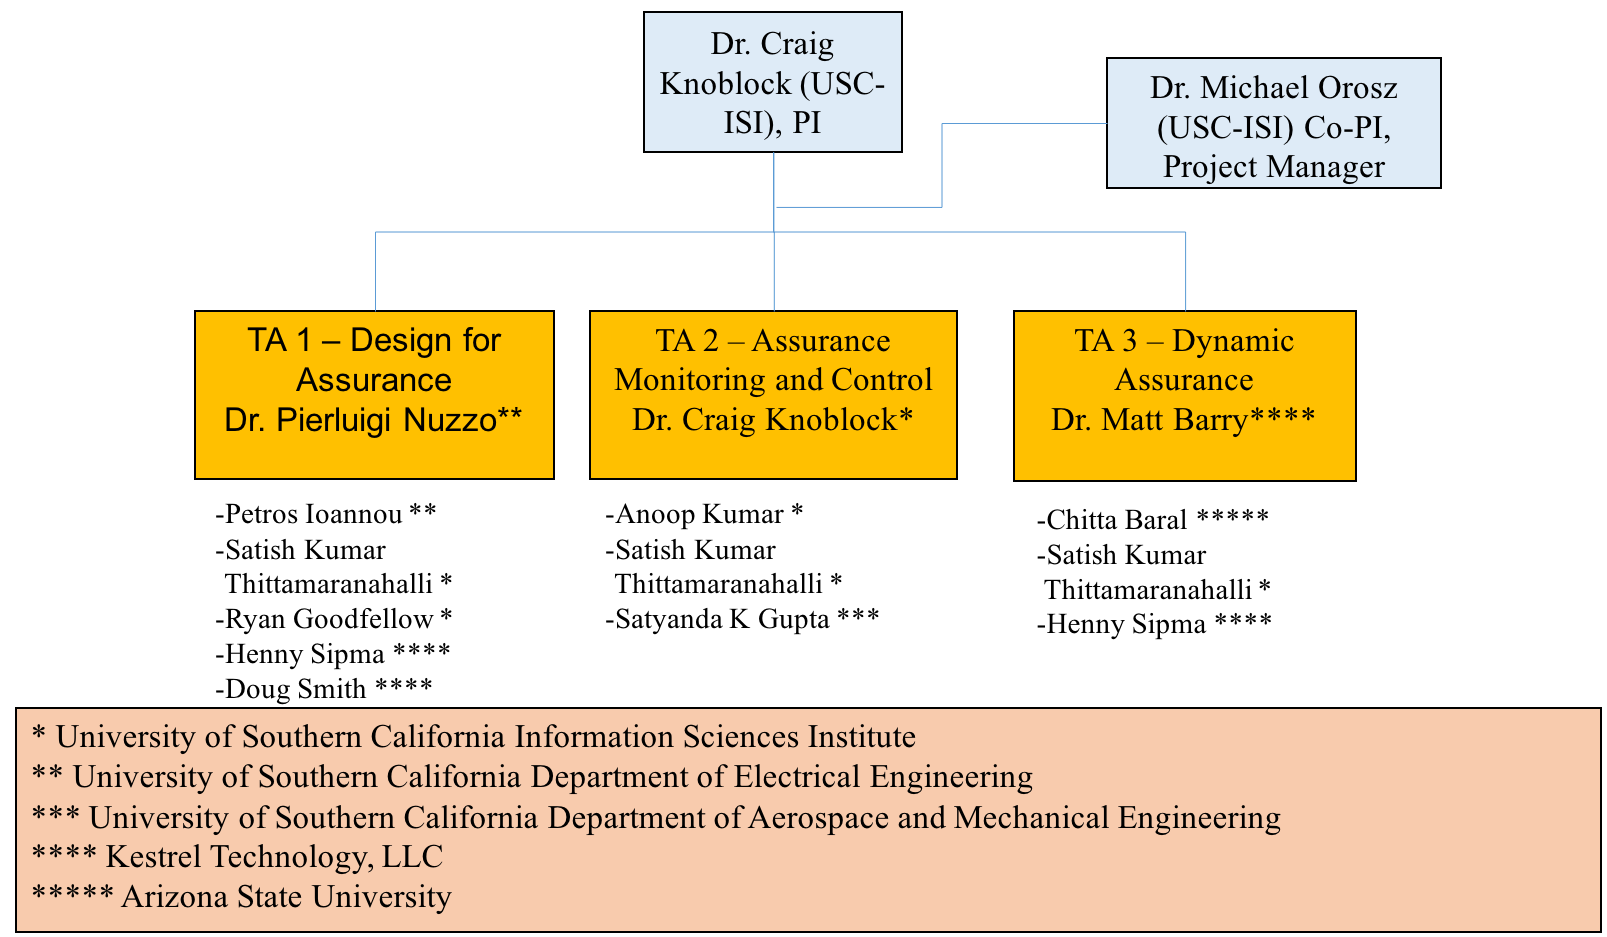
\includegraphics[width=6.0in]{./org-chart2.png}
\caption{\small Organization Chart}
\label{fig:org_chart}
\end{figure}

Coordination: To maximize collaboration and reduce risk to project failure from lack of communication and technical exchange, we plan to employ a wide variety of working styles and communication/coordination so that all can contribute.  At the core of our project will be regularly scheduled meetings bridging the diversely distributed team (Table~\ref{fig:Collaboration_Table}).  These meetings will address project status, identify challenges, implement risk mitigation strategies and participate in technology exchanges and system integration efforts (when appropriate)

\begin{table}[ht]
\caption{\small Project Meetings and Events}
  \centering
  {\footnotesize
\begin{tabular}{|m{3.15in}|m{3in}|} 
\hline
\textbf{Meeting} & \textbf{Frequency} 
\\\hline
Conference calls among investigators (discuss project status, address concerns and project risks) & Weekly
\\
\hline
Technical exchange and coordination meetings using Bluejeans or another videoconference technology & At least twice a month and more frequently as needed
  \\ 
\hline
Face-to-Face meetings (prior to P/I and demonstration meetings) & Every 3 to 6 months and more frequently (especially at the beginning of the project) as needed
 \\\cline{1-2}

\hline
\end{tabular}
}
\label{fig:Collaboration_Table}
\end{table}

\begin{table}[tbhp]
\caption{\small Key Project Team Member Responsibilities}
  \centering
  {\footnotesize
\begin{tabular}{| m{.75in} | m{3.9in}| m{1.5in}|} 
\hline
\textbf{Key Member} & \textbf{Responsibilities} & \textbf{Tasks} 
\\\hline
Dr.\ Craig Knoblock  & Principal Investigator responsible for project, leads TA 2 – Assurance Monitoring and Control.  Will lead the overall project and lead the TA2 team.  Served as the PI on many DARPA projects and has sucessfully led many large teams.    Effort on project:  25\% &
1.1.6, 1.2.2 1.2.3, 1.2.4, 1.3.4, 1.4.1, 
2.1.6, 2.2.2 2.2.3, 2.2.4, 2.3.4, 2.4.1, 
3.1.6, 3.2.2, 3.2.3, 3.2.4, 3.3.4, 3.4.1
\\
\hline
Dr.\ Michael Orosz & Co-Principal Investigator responsible managing the day-to-day operations of the project, assist technical teams as needed, coordinate with TA4 teams.    Has led many large complex multi-disciplined/multi-organizational projects in academic and industry environments.  Effort on project: 50\%
& 1.1.6, 2.1.6, 3.1.6, 1.4.1, 2.4.1, 3.4.1
  \\ 
\hline
Dr.\ Pierluigi Nuzzo 
& 
Co-Principal Investigator.  Leads the TA 1 - Design for Assurance team and conducts research on the formal methods for the design of the TA1 system.  Research experience on methodologies and tools for the design of cyber-physical systems; contracts, interfaces, and compositional methods for embedded system design; the application of automated formal methods and optimization theory to problems in embedded and cyber-physical systems.  Effort on project: 2 months/year (16.6\%)
& 
1.1.1, 2.1.1, 3.1.1 \\
\hline
Dr.\ Matthew Barry
& 
Key personnel.  Leads the TA 3 – Dynamic Assurance.   He will conduct the research on the dynamic assurance case language editors and parsers, the run-time system, and system integrations. Effort on project:  66\%
& 
1.3.2, 2.3.2, 3.3.2\\
\hline
Dr.\ Chitta Baral
& 
Key personnel responsible for learning assurance rules, supporting assurance rules with uncertainty and improving solver speed.  Expertise on ASP solvers, which will be used to reason about the assurance cases. Effort on project: 20\%
& 
1.3.1, 2.3.1, 3.3.1 \\
\hline
Dr.\ Doug Smith 
& 
Key personnel will support formal methods aspects of TA1, and lead the effort on abstract refinement. Expertise in field of automated correct-by-construction program generation.    Effort on project: 40\%
& 
1.1.5, 2.1.5, 3.1.5 \\
\hline
Dr.\ Henny Sipma
& 
Key personnel who will support the program verification tasks under TA1.  Will lead the effort on program verification.   Effort on project:  45\%
& 
1.1.5, 2.1.5, 3.1.5, 1.3.2, 2.3.2, 3.3.2 \\
\hline
Dr.\ Petros Ioannou
& 
Key personnel responsible providing and extending the assurance test bed, which will be available at the start of the project for autonomous vehicles.   Effort on project: 1 month/year (8.3\%)
& 
1.1.2, 2.1.2 (optional), 3.1.2 (optional)
\\
\hline
Dr.\ Satyandra Kumar Gupta
& 
Key Personnel providing autonomous command and control expertise to the TA-2 team.   Will lead the research on safety aware learning on TA2.   Past research on physics-aware decision making to facilitate automation.  Effort on project: 1 month/year (8.3\%)
& 
1.2.1, 2.2.1, 3.2.1 \\
\hline
Dr.\ Anoop Kumar 
& 
Key personnel providing support to the TA 2 project team.  Will lead the research on monitoring \& control and detecting distribution shifts.  Effort on project: 50\%
& 
1.2.1, 1.2.2, 1.2.3, 1.2.4, 2.2.1, 2.2.2, 2.2.3, 2.2.4, 3.2.1, 3.2.2, 3.2.3, 3.2.4\\
\hline
Dr.\ Satish Thittamaranahalli
& 
Key personnel developing scalable algorithms for TA1, TA2, and TA3 project teams.  Has extensive experience on scalable algorithm design, machine learning, and constraint reasoning.  Effort on project: 50\%
& 
1.2.1, 1.2.2, 1.2.3, 1.2.4, 2.2.1, 2.2.2, 2.2.3, 2.2.4, 3.2.1, 3.2.2, 3.2.3, 3.2.4, 1.1.4, 2.1.4, 3.1.4 \\
\hline
Dr.\ Ryan Goodfellow
& 
Key personnel providing support to the TA-1 project. Will lead the research on simulation-based testing.  Has extensive experience on simulation-based testing.  Effort on project:  30\%
& 
1.1.3, 2.1.3, 3.1.3 \\

\cline{1-2}

\hline
\end{tabular}
}
\label{fig:Table_Mgmt}
\end{table}



\newpage
\section{Personnel, Qualifications and Commitment}

{\bf Dr.\ Craig Knoblock}, the PI on this effort, is a Research Professor of both Computer Science and Spatial Sciences at the University of Southern California (USC) and Director of the Intelligent Systems Division at the USC Information Sciences Institute.   He received his Ph.D. from Carnegie Mellon University in computer science. 
%His research focuses on techniques for describing, acquiring, and exploiting the semantics of data.  
In previous projects he has worked on developing  scalable approaches to execution monitoring, accurate detection of sensor failures, and   automatic modeling and reconstruction of sensors.  He has published more than 300 journal articles, book chapters, and conference papers on these topics.  Dr. Knoblock is a Fellow of the Association for the Advancement of Artificial Intelligence (AAAI), a Distinguished Scientist of the Association of Computing Machinery (ACM), a Senior Member of IEEE, past President and Trustee of the International Joint Conference on Artificial Intelligence.
%and winner of the 2014 Robert S. Engelmore Award.  

{\bf Dr.\ Michael Orosz}, a Co-PI on this effort, is a Research Associate Professor of Civil and Environmental Engineering at the University of Southern California (USC) and Research Director of the Decision Systems Group at the USC Information Sciences Institute.  Dr. Orosz has over 30 years’ experience in commercial and government software development, basic and applied research, project management, academic research and has developed and deployed several commercially successful products.  His research interests are in machine learning and decision analytics as applied to intelligence analysis and autonomous command and control such as smart building controls.    Dr. Orosz has extensive experience in managing large complex multi-disciplined/multi-teamed research projects. %funded by DARPA, DHS, DoD, DoE, Industry, NASA, NRO, NSA and ONR.   
He received his Ph.D. in computer science from the University of California, Los Angeles.

{\bf Dr.\ Pierluigi Nuzzo}, a Co-PI on this project, is an Assistant Professor in the Department of Electrical Engineering at the University of Southern California. He received the Ph.D. in Electrical Engineering and Computer Sciences from the University of California at Berkeley. 
%in 2015, and the Laurea degree (MS) in electrical engineering (summa cum laude) from the University of Pisa, Italy, and the Sant'Anna School of Advanced Studies, Pisa, Italy.
%
%He has four years of research experience in analog and mixed signal circuit design as a researcher at IMEC, Leuven, Belgium, and over 10 years experience in design methodologies and tools for mixed-signal integrated circuits and cyber-physical systems, as a researcher at the University of Pisa, IMEC, UC Berkeley, and USC. 
His research interests
include: methodologies and tools for cyber-physical system and mixed-signal
system design; contracts, interfaces and compositional methods for embedded
system design; the application of formal methods and optimization theory to problems in embedded and cyber-physical systems and electronic design automation. 
%
Prof. Nuzzo received %First Place in the operational category and Best Overall
%Submission in the 2006 DAC/ISSCC Design Competition, 
a Marie Curie Fellowship
from the European Union in 2006, 
the University of California at Berkeley EECS
departmental fellowship in 2008, 
%the University of California at Berkeley Outstanding Graduate Student Instructor Award in 2013, 
the IBM Ph.D.
Fellowship in 2012 and 2014, 
%the Best Paper Award from the International Conference on Cyber-Physical Systems (ICCPS) in 2016, 
and the David J.~Sakrison Memorial Prize in 2016 for his doctoral research. 
%He is an author of 1 patent and over 60 publications.

{\bf Dr.\ Satyandra K. Gupta} is Smith International Professor in the Department of Aerospace and Mechanical Engineering at the University of Southern California. %Prior to joining the University of Southern California, he was a Professor in the Department of Mechanical Engineering and the Institute for Systems Research at the University of Maryland. He was the founding director of the Maryland Robotics Center and the Advanced Manufacturing Laboratory at the University of Maryland. 
He served as a program director for the National Robotics Initiative at the National Science Foundation from September 2012 to September 2014.  Dr. Gupta's interest is in the area of physics-aware decision making to facilitate automation. He has published more than 300 technical articles. He is a fellow of the American Society of Mechanical Engineers (ASME) and editor of ASME Journal of Computing and Information Science in Engineering. Dr. Gupta has received the Young Investigator Award from the Office of Naval Research in 2000, CAREER Award from the National Science Foundation in 2001, Presidential Early Career Award for Scientists and Engineers (PECASE) in 2001, Invention of the Year Award at the University of Maryland in 2007, Kos Ishii-Toshiba Award from ASME in 2011, and Excellence in Research Award from ASME in 2013.%, and Distinguished Alumnus Award from Indian Institute of Technology, Roorkee in 2014. %He has also received seven best paper awards at conferences.

{\bf Ryan Goodfellow} is a computer scientist at ISI working in combined cyber physical simulation and emulation platform development. His formal background is in simulation algorithms and modeling techniques using differential-algebraic equations (DAE). He has applied this knowledge in the CPS space by integrating DAE modeling languages and simulation engines with network testbeds to create comprehensive scientific experimentation platforms for cyber-physical systems. These experimentation platforms have been used in the power grid research space. %Ryan is a lead developer on the Deter network testbed, with a strong background in networked and distributed systems engineering. %He is also a combat veteran, serving as a non-commissioned officer and SIGINT team lead for a multi-functional intelligence team in Afghanistan.

{\bf Dr.\ Petros Ioannou} is a Professor in the Department of Electrical Engineering, Director of the Center for Advanced Transportation Technologies and Associate Director for Research for the DOT supported University Transportation Center at USC. He received his MS and PhD from the University of Illinois at Urbana Champaign in Mechanical and Electrical Engineering, respectively. His research interests are in robust adaptive control, vehicle dynamics and control, human factors and safety, automated vehicles, nonlinear systems and Intelligent transportation Systems.  He received the 2016 IEEE Transportation Technologies field award and the 2016 IEEE Control system society Transition to Practice Award. He is a Fellow of IEEE, IFAC and IET and author/coauthor of 8 books and over 400 papers.

{\bf Dr.\ Matthew Barry} will serve as lead for the TA3 tasks. %He will implement the dynamic assurance case language editors and parsers, the run-time system, and system integrations.  He will implement the assurance case arguments and the API for updating argument structure and content.  
Dr. Barry currently is CEO at Kestrel Technology LLC, and previously spent 20 years in NASA space mission operations at the Jet Propulsion Lab and Johnson Space Center.  At NASA Headquarters he led the introduction of dependability case requirements and plans for flight computing systems in upcoming manned space exploration missions, as well as the development of Agency-level software-related safety-critical control system requirements.  He recently served as a Principal Investigator on DHS/Cyber S\&T STAMP (Static Tool Analysis Modernization Program), DARPA CSFV (Crowd Sourced Formal Verification), three NASA Aeronautics R\&D projects, and the AFRL-sponsored Static Analysis of Numerical Algorithms project.  Dr. Barry earned BSME, MS, and PhD degrees in mechanical engineering, and an MBA degree, from Rice University.  

{\bf Dr.\ Henny Sipma} will support the program verification tasks under TA1.  %She is the key person behind the company's {\em KT Advance\/} and {\em KT Transferal\/} static analysis products, and the designer and programmer of the company's core {\em CodeHawk\/} abstract interpretation engine. 
Dr. Sipma currently is the CTO at Kestrel Technology LLC.  She has spent the past 10 years with Kestrel Technology as a static analysis expert; previously developed and taught static analysis techniques as senior research associate at Stanford University for eight years; and developed industrial process controls as an senior systems analyst at Shell.  She has been Principal Investigator or company lead on several recent R\&D projects for Federal agencies, including two projects under the IARPA STONESOUP (Securely Taking On New Executable Software of Uncertain Provenance) program; the DHS Cyber S\&T Gold Standard project; and the DARPA-sponsored STAC (Space-Time Analysis for Cybersecurity) and MUSE (Mining and Understanding Software Enclaves) programs.  Dr. Sipma earned 
%a BS degree in chemistry and an MS degree in chemical engineering at the University of Groningen in The Netherlands, and 
MS and PhD degrees in computer science from Stanford University.  

{\bf Dr.\ Douglas R.\ Smith} will support formal methods aspects of TA1, including the enforcement of safety properties and the generation of monitors.  He is President of Kestrel Technology LLC and Principal Scientist at Kestrel Institute.  He is a Fellow of the American Association of Artificial Intelligence (AAAI) and an ASE Fellow (Automated Software Engineering).  From 1986 to 2000, he taught an advanced graduate course on correct-by-construction software development at Stanford.  
%Dr. Smith has led the development of a series of software synthesis systems, including KIDS (Kestrel Interactive Development System), Specware, Designware, and Planware. 
%Applications domains have included a variety of complex high-performance planners and schedulers for the US Air Force.  He leads current projects on the generation of air mission plans and cyberoperations.  
Other recent projects focused on automated policy enforcement \cite{SmithD0703,SmithD08}, synthesis of secure network protocol codes, and the synthesis of high-performance constraint-solvers\cite{SmithD08c,SmithD13}.  Dr. Smith has over 30 years experience in the field of automated correct-by-construction program generation and has published over 100 papers. He has one patent.  He received the Ph.D. in Computer Science from Duke University% in 1979.  

{\bf Dr. Chitta Baral} is a Professor in the Department of Computer Science and Engineering at Arizona State University. He will support the TA3 efforts on Learning assurance rules, supporting assurance rules with uncertainty and improving solver speed. Dr. Baral has expertise in various aspects of autonomy and Artificial Intelligence. 
He wrote the first book on answer set programming (published by Cambridge University Press) the formal language behind our assurance rules. Some of his other works relevant to this proposal are: goal specification for autonomous systems, automatic construction of control rules for autonomous systems that satisfy given goals, combining machine learning with reasoning in various contexts, including image understanding. %He is the President of KR Inc. He is an associate editor of AIJ and has been an associate editor of JAIR.

{\bf Dr.\ Satish Kumar Thittamaranahalli (T. K. Satish Kumar)} leads the Collaboratory for Algorithmic Techniques and Artificial Intelligence (CATAI) at USC's Information Sciences Institute. He has published over 60 papers on numerous topics in Artificial Intelligence spanning such diverse areas as Constraint Reasoning, Planning and Scheduling, Probabilistic Reasoning, Robotics, Combinatorial Optimization, Approximation and Randomization, Heuristic Search, Model-Based Reasoning, Knowledge Representation and Spatio-Temporal Reasoning. %He %has served on the Program Committees of many international conferences in Artificial Intelligence
He and is a winner of the 2016 Best Robotics Paper Award and the 2005 Best Student Paper Award from the International Conference on Automated Planning and Scheduling. 
Dr. Kumar received his PhD in Computer Science from Stanford University. %In the past, he has also been a Visiting Student at the NASA Ames Research Center, a Postdoctoral Research Scholar at the University of California, Berkeley, a Research Scientist at the Institute for Human and Machine Cognition, a Visiting Assistant Professor at the University of West Florida, and a Senior Research and Development Scientist at Mission Critical Technologies.

\textbf{Dr.\ Anoop Kumar} is a senior computer scientist at USC ISI and has broad expertise in machine learning, statistical modeling, and software engineering.  Dr.\ Kumar is the technical lead on the DARPA RSPACE program and has played a vital role in developing a system that fuses air operations data from multiple sources, maintains world state, and issues warnings. Previously, he led the research and development of the BBN’s election forecasting system for the IARPA OSI program. %Dr.\ Kumar played a significant role in the DARPA DEFT program by developing a model to support integration of output from multiple NLP algorithms. He has contributed at the development to management levels on government research contracts and commercial projects. 
Dr.\ Kumar helped design and develop BBN's commercially available, hosted speech and medical transcription services offering. 

\begin{table}[!tbh]
\begin{footnotesize}
\vspace{-0.1in}

\begin{tabular}{lll}
\begin{tabular}[t]{|l|@{}c@{}|@{}c@{}|@{}c@{}|@{}c@{}|} \hline
Project & Status & \multicolumn{3}{ c| }{Hours} \\ \cline{3-5}
& & P1 & P2 & P3 \\ \hline



\multicolumn{5}{ |c| }{ \textbf{Craig Knoblock} } \\ \cline{1-5}
Safeguard & Pro & 770 & 641 & 641 \\ \cline{1-5}
ELICIT & Cur & 308 & 256 & 120 \\ \cline{1-5}
WTNIC & Cur & 11 & 0 & 0 \\ \cline{1-5}
EFFECT & Cur & 641 & 107 & 0 \\ \cline{1-5}
LinkedMaps & Cur & 203 & 25 & 0 \\ \cline{1-5}
PRINCESS & Cur & 608 & 96 & 0 \\ \cline{1-5}
SCHARP & Cur & 481 & 54 & 0 \\ \cline{1-5}
MINT & Pen & 650 & 534 & 285 \\ \cline{1-5}

\multicolumn{5}{ |c| }{ \textbf{Michael Orosz} } \\ \cline{1-5}
Safeguard & Pro & 1560 & 1300 & 1300  \\ \cline{1-5}
SMC/SY & Cur & 1803 & 0 & 0  \\ \cline{1-5}

\multicolumn{5}{ |c| }{ \textbf{Matthew Barry} } \\ \cline{1-5}
Safeguard & Pro & 2078 & 1690 & 1554 \\ \cline{1-5}
Starlite & Cur & 1840 & 1692 & 0 \\ \cline{1-5}



\multicolumn{5}{ |c| }{ \textbf{Anoop Kumar} } \\ \cline{1-5}
Safeguard & Pro & 1560 & 1300 & 1300 \\ \cline{1-5}

\end{tabular}
&
\begin{tabular}[t]{|l|@{}c@{}|@{}c@{}|@{}c@{}|@{}c@{}|} \hline
Project & Status & \multicolumn{3}{ c| }{Hours} \\ \cline{3-5}
& & P1 & P2 & P3 \\ \hline

\multicolumn{5}{ |c| }{ \textbf{Pierluigi Nuzzo} } \\ \cline{1-5}
Safeguard & Pro & 520 & 433 & 433  \\ \cline{1-5}
Mirage & Cur & 433 & 0 & 0  \\ \cline{1-5}

\multicolumn{5}{ |c| }{ \textbf{Satyandra Gupta} } \\ \cline{1-5}
Safeguard & Pro & 260 & 217 & 217 \\ \cline{1-5}
Human   & Cur & 22 & 0 & 0 \\ \cline{1-5}
Vehicles & Cur & 36 & 0 & 0 \\ \cline{1-5}
Robot & Cur & 116 & 0 & 0 \\ \cline{1-5}
Assembly & Cur & 33 & 0 & 0 \\ \cline{1-5}
Solar & Cur & 4 & 0 & 0 \\ \cline{1-5}

\multicolumn{5}{ |c| }{ \textbf{Petros Ioannou} } \\ \cline{1-5}
Safeguard & Pro & 260 & 217 & 217 \\ \cline{1-5}
CPS & Cur & 130 & 0 & 0 \\ \cline{1-5}

\multicolumn{5}{ |c| }{ \textbf{Ryan Goodfellow} } \\ \cline{1-5}
Safeguard & Pro & 936 & 780 & 780 \\ \cline{1-5}
STEAM & Cur & 416 & 0 & 0 \\ \cline{1-5}


\end{tabular}
&
\begin{tabular}[t]{|l|@{}c@{}|@{}c@{}|@{}c@{}|@{}c@{}|} \hline
Project & Status & \multicolumn{3}{ c| }{Hours} \\ \cline{3-5}
& & P1 & P2 & P3 \\ \hline

\multicolumn{5}{ |c| }{ \textbf{Chitta Baral} } \\ \cline{1-5}
Safeguard & Pro & 659 & 485 & 485 \\ \cline{1-5}
PostdocBP & Cur & 176 & 0 & 0 \\ \cline{1-5}
Languages & Pen & 528 & 264 & 264 \\ \cline{1-5}
CAREER & Pen & 88 & 44 & 44 \\ \cline{1-5}
CHS & Pen & 510 & 255 & 0 \\ \cline{1-5}

\multicolumn{5}{ |c| }{ \textbf{Doug Smith} } \\ \cline{1-5}
Safeguard & Pro & 1222 & 984 & 840 \\ \cline{1-5}
RSPACE & Cur & 342 & 0 & 0 \\ 
\cline{1-5}
PLANX & Cur & 154 & 0 & 0 \\ 
\cline{1-5}
HACCS & Pen & 923 & 769 & 769 \\ 
\cline{1-5}

\multicolumn{5}{ |c| }{ \textbf{Henny Sipma} } \\ \cline{1-5}
Safeguard & Pro & 1372 & 962 & 840 \\ \cline{1-5}
STAC & Cur & 797 & 0 & 0 \\ \cline{1-5}

\multicolumn{5}{ |c| }{ \textbf{Satish Thittamaranahalli} } \\ \cline{1-5}
Safeguard & Pro & 1560 & 1300 & 1300 \\ \cline{1-5}
MapF & Cur & 103 & 103 & 0 \\ \cline{1-5}

\end{tabular}
\end{tabular}

\end{footnotesize}
\caption{Individual commitments of key personnel}
\label{tab:Commitments}
\vspace{-0.2in}
\end{table}

\clearpage
\newpage
\section{Capabilities}


%\subsection{University of Southern California}
USC has strengths in number of areas that are closely related to the proposed work:
\begin{itemize}[itemsep=0pt,leftmargin=*]
\item Dr.\ Nuzzo 
%has over 10-year research experience in embedded system design, from mixed-signal chip design (analog-to-digital converters, frequency synthesizers, software-defined radio), to methodologies and tools for mixed-signal integrated circuits and Cyber-Physical Systems (CPSs), and the application of formal methods and optimization theory to problems in embedded and cyber-physical systems and electronic design automation.  
%His doctoral work 
has done extensive research on contracts and compositional methods for heterogeneous system design and design space exploration, with application to aircraft electric power systems and environmental control systems. His work has helped transition rigorous system design foundations, innovative design methodologies, and new systems engineering paradigms to industry (IBM, United Technologies). 
\item Dr.\ Satyandra K. Gupta has worked on autonomous surface vehicles, autonomous ground vehicles for operation on rugged terrains, and autonomous flapping wing aerial vehicles.   His group has developed a hierarchal decision making approach for realizing autonomous systems. 
%This approach combines task planning and assignment, deliberative trajectory planning, reactive collision avoidance behaviors, and trajectory tracking control layers. 
His group has also developed new methods for learning reactive behaviors in adversarial environments and COLREGS compliant trajectory planning. \item Dr.\ Knoblock has developed methods that learn the relationships between sensors to both identify failures and changes in sensor and reconstruct those sensors, providing estimates of the accuracy of the reconstructed sensors.  
\item Ryan Goodfellow has extensive experience in simulation based testing through high-fidelity CPS testbed environment development and operation, using the Deter network testbed as the core which has supported several large scale government projects from a variety of agencies and thousands of users. %we have developed sophisticated CPS experiments under programs such as NFS RIPS, NIST SmartCities and the DHS Cybersecurity showcase.
\item Dr.\ Ioannou %helped  design and implement adaptive cruise control systems in collaboration with Ford Motor Company, which was commercialized four years before any other company. He 
worked on several DOT funded projects on automated vehicles and intelligent highway systems where he demonstrated his vehicle control designs for safety and performance on actual automated vehicles in test trucks and I-15 highway.
\item Drs.\ Knoblock, Kumar, and Thittamaranahalli have developed highly scalable approaches for monitoring message traffic to identify potential problems and issue warnings and alerts. 
\item Dr. Thittamaranahalli has developed state-of-the-art methods for efficiently solving large-scale search and optimization problems. %These techniques will be applicable in TA2 for safety-aware learning and planning, in TA2 for assurance monitoring and control, and in TA3 for dynamic assessment of assurance cases.

\end{itemize}
%\subsection{Kestrel Technology LLC}

Kestrel Technology's strength is in program analysis, specifically static analysis of both source and binary targets.  The company performs applied R\&D and product development for a variety of static analysis applications  pivoting primarily on the abstract interpretation technique.  The company recently initiated development of program analysis applications using logical equivalence techniques. As a provider of verification evidence in the form of mathematical proofs, the company also has expertise in the design and development of assurance case arguments for high-integrity systems using such evidence. %The company is engaged in a partnership with Wind River Systems to develop program analysis tools for its embedded system developers.  Many of Wind River's customers must develop their products under safety and certification standards, including those using safety cases.  

   

%\subsection{Arizona State University}
Chitta Baral at Arizona State University has developed various software to learn assurance rules and various ASP solvers, which he has made available as open-source.

Most of the software carried forward for implementation or derivation is open source.  The single exception is Kestrel Technology's {\it KT Advance\/} static analysis tool (TA1), in particular the abstract interpretation engine therein, which is company proprietary and is US EAR export-controlled.   
%Owing to mixed funding for the development of that technology 
We will continue to provide the Federal government a restricted use license for that particular item.

There are no specialized facilities, data, or GFE required for this effort. 

\include{sow}
\include{milestones}

% \section{Level of Effort by Task \textcolor{red}{[Mike/Lisa - 1 pages]}}

% \textcolor{blue}{
% \begin{itemize}
% \item Will be a separate spreadsheet
% \item
% \end{itemize}
% }

\include{appendix_a}

%\section{Appendix B \textcolor{red}{[No Page Count]}}

\section{References}
\bibliographystyle{acm} 
\bibliography{TA3/ta3,TA2/ta2,TA1/ta1}
\end{document}
%%\documentclass[a4paper]{article}
%\documentclass[12pt]{article}
\documentclass[12pt]{dod-blank}

%% Language and font encodings
\usepackage[english]{babel}
\usepackage[utf8x]{inputenc}
\usepackage[T1]{fontenc}

%% Sets page size and margins
%%\usepackage[a4paper,top=3cm,bottom=2cm,left=3cm,right=3cm,marginparwidth=1.75cm]{geometry}
%\usepackage[top=1in, bottom=1in, left=1in, right=1in]{geometry}



%% Useful packages
\usepackage{amsmath}
\usepackage{graphicx}
  \graphicspath{{.}{./image/}}
  \DeclareGraphicsExtensions{.png,.jpg} 
\usepackage[colorinlistoftodos]{todonotes}
\usepackage[colorlinks=true, allcolors=blue]{hyperref}
\usepackage{tabularx}
\usepackage{multirow}
\usepackage{tabulary}
\usepackage{float}
\usepackage{wrapfig}
\usepackage[export]{adjustbox}
\usepackage{comment}
\usepackage{tabularx}
\usepackage{multirow}
\usepackage{tabulary}
\usepackage{enumitem}

\usepackage{listings}
\usepackage{color}
\usepackage{array}
\usepackage{subcaption}
\usepackage{xcolor}




\renewcommand{\textfraction}{0}
\renewcommand{\topfraction}{1.0}
\renewcommand{\bottomfraction}{1.0}

\usepackage{longtable}
%% macros
\newif\iffinal
\finaltrue
\iffinal
  
    \newcommand\baareq[1]{}
    \newcommand\baades[1]{}
 
 
\else
    \definecolor{darkgreen}{rgb}{0,0.4,0}
    \definecolor{darkcyan}{rgb}{0,0.4,0.4}
    \definecolor{darkblue}{rgb}{0,0,0.5}
    
    \newcommand\baareq[1]{{\color{darkcyan}[\textbf{Requirement:} #1]}}
    \newcommand\baades[1]{{\color{darkcyan}[\textbf{Description:} #1]}}
 
\fi




\def\naive{na\"{\i}ve}



\lstset{ 
  backgroundcolor=\color{white},   % choose the background color; you must add \usepackage{color} or \usepackage{xcolor}
  basicstyle=\footnotesize\ttfamily,            % the size of the fonts that are used for the code
  breakatwhitespace=false,         % sets if automatic breaks should only happen at whitespace
  breaklines=true,                 % sets automatic line breaking
  captionpos=b,                    % sets the caption-position to bottom
  commentstyle=\color{mygreen},    % comment style
  % deletekeywords={...},            % if you want to delete keywords from the given language
  escapeinside={\%*}{*)},          % if you want to add LaTeX within your code
  extendedchars=true,              % lets you use non-ASCII characters; for 8-bits encodings only, does not work with UTF-8
  frame=single,	                   % adds a frame around the code
  keepspaces=false,                 % keeps spaces in text, useful for keeping indentation of code (possibly needs columns=flexible)
  keywordstyle=\color{blue}\bfseries\underbar,       % keyword style
  language=Prolog,                 % the language of the code
  % morekeywords={if,and},        % if you want to add more keywords to the set
  numbers=none,                    % where to put the line-numbers; possible values are (none, left, right)
  numbersep=5pt,                   % how far the line-numbers are from the code
  numberstyle=\tiny\color{mygray}, % the style that is used for the line-numbers
  rulecolor=\color{black},         % if not set, the frame-color may be changed on line-breaks within not-black text
  showspaces=false,                % show spaces everywhere adding particular underscores; it overrides 'showstringspaces'
  showstringspaces=false,          % underline spaces within strings only
  showtabs=false,                  % show tabs within strings adding particular underscores
  stepnumber=2,                    % the step between two line-numbers. If it's 1, each line will be numbered
  stringstyle=\color{mymauve},     % string literal style
  tabsize=2,	                   % sets default tabsize to 2 spaces
  title=\lstname                   % show the filename of files included with \lstinputlisting; also try caption instead of title
}

% apply trick for additional keywords for our AC DSL
\lstset{
	emph={for, if, and, or},
    emphstyle={\color{blue}\bfseries\underbar}
}




\title{DARPA Assured Autonomy}
\author{Technical Volume- \textcolor{red}{Thirty-Eight (38) pages max}}

\begin{document}
\pagenumbering{roman}
\include{cover}

\newpage
\section{Table of Contents}
\tableofcontents

\newpage
\pagenumbering{arabic}
\section{Executive Summary}
As we rapidly move into a world where machine learning plays a central role in realizing autonomous systems, it is becoming increasingly important to develop techniques that assure that these systems will operate safely and perform as expected. Current approaches are limited to providing assurance for systems with limited or no  learning capabilities. In this context, DARPA's Assured Autonomy BAA seeks to \emph{develop rigorous design and analysis technologies for continual assurance of learning-enabled autonomous systems}. USC in collaboration with Kestrel Technology and ASU is pleased to submit a comprehensive TA1, TA2, and TA3 proposal entitled \emph{``Assured Autonomy for Learning Enabled Vehicles (Safeguard).''} We plan to provide an end-to-end solution to support autonomous systems with learning-enabled components, ranging from design technologies for assurance, to assurance monitoring and control techniques, to representation and online evaluation of assurance cases. We have assembled a strong team of experts that cover the range of technologies that are required to create such an end-to-end system. If successful, the project will provide the technologies for building the next-generation of learning-enabled autonomous systems.  The entire project will take four years and cost \textcolor{red}{\$??}, with an initial version completed at the end of Phase I and successive versions with additional capabilities and improved scalability at the end of Phase II and Phase III.  

In the remainder of this section, we first introduce an  unmanned surface vehicle scenario that will be used throughout the proposal to describe the approach.  Next, we describe our approach to design, monitoring, and dynamic assurance. Finally, we introduce the team involved in the project. 

\textbf{Motivating Scenario.} Consider an autonomous unmanned surface vehicle (USV) guarding a valuable asset in the ocean when an unknown vehicle  approaches the security perimeter, under challenging weather conditions. In this scenario, the USV is required to approach the intruding vehicle, issue a warning signal, and escort it to a safe distance from the controlled area. However, as the USV has no a priori knowledge of its external environment behaviors (e.g., water depth, waves, wind, current, visibility), pre-computing a feasible trajectory, let alone optimal, becomes a non-trivial problem. For trajectory planning, the USV must continuously perform the following tasks:
\begin{itemize}[itemsep=0pt,leftmargin=*]
 \item Sense the current state of the surrounding environment (e.g., water depth, waves, wind, current, visibility) and estimate its own maneuverability constraints (e.g., braking distance, available acceleration, maximum velocity, turning radius, turning rate, safety distance) based on the state of the environment;      
\item Sense the static obstacles in the sensor range and generate a traversability map;
\item Sense the moving obstacles and classify them;   
\item Predict future trajectories of moving obstacles; 
\item Determine if any of the COLREGS \cite{commandant1999international} rules will be in effect with respect to one or more of the nearby vessels and identify the vessels with the right of way.    
\end{itemize}
The above information will be used by the trajectory planner to compute an initial trajectory, which will be continuously refined as the USV gathers additional information.
% It is not possible for the USV to be tested in every possible environment. 
The USV will use learning enabled components to take  decisions as it encounters new situations, such as  
\begin{itemize}[itemsep=0pt,leftmargin=*]
\item Classifiers to identify moving obstacles based on physical appearance and motion signatures,
\item Algorithms to estimate the sensor capabilities in adverse weather conditions,   
\item Algorithms to accurately estimate uncertainty in the environment, 
\item Classifiers to generate traversability maps,
\item Prediction of external vessel behaviors based on motion histories, 
\item Reinforcement learning  to ensure COLREGS compliance of maneuvers,  
\item Algorithms to learning pursuit behaviors.  
\end{itemize}
Learning enabled components will interact with each other in complex ways, where a misclassification error in one component may eventually compromise the entire mission.   
% We will need to make sure that each learning enabled components has a run-time monitor that will ensure that the assumptions made by the learning-enabled component remain valid and prevent erroneous learning. 
% For example, if the vehicle is exhibiting significant error in trajectory tracking, then simply downgrading the trajectory tracking error value may not be a good option.  The failure of prediction of trajectory tracking error might be due to the presence of a significant wake caused by a nearby vessel. The presence of the nearby vessel can be used to explain the degradation in trajectory tracking performance. As the vessel moves away, we can expect the trajectory tracking performance to return to the predicted level.  
While exhaustive validation of learning-enabled cyber-physical systems (LE-CPSs) is a prohibitive task~\cite{Kalra16},
their complexity, heterogeneity, and highly dynamic nature
make it challenging to even leverage existing model-based development techniques to effectively assess system correctness 
% dependability, 
at design time or enforce it at runtime.

\textbf{Design for Assurance.} Safeguard uses a platform-based design approach~\cite{Nuzzo15b} to organize the design process for a LE-CPS and to build assurance cases. Composite models are developed at several levels of abstraction,
from top-level system requirements and safety constraints down to the
implementation level.  Intermediate levels add detail to the levels
above.  The different levels are connected by refinement mappings that
allow properties established at one level to be preserved at the next
level (see Figures~\ref{fig:methodology} and~\ref{fig:assurance}).

Contracts are used to formally specify components and composite models
in terms of (1) Assumptions -- the assumed behaviors of the
environment and the behaviors of other components, and (2) Guarantees
-- the behavior properties that a model guarantees if it operates in a
context that satisfies its assumptions.  A calculus of contracts
allows horizontal composition of contracts to generate contracts for
composite models.  Vertical contracts are used to specify the mapping
or refinement relation between models at different levels of
abstraction.  The system design process starts with a high-level
contract that expresses overall system assumptions and requirements.
Subsequent levels express models with increasing detail until the
lowest level expresses the system in terms of hardware components and
their software controllers.

The assurance case for a CPS arises from the horizontal and vertical
structure of the design in several ways.  The components used within a
particular level are either (1) synthesized using
correct-by-construction design tools together with proofs, (2) derived
statically or dynamically using safety-aware machine-learning
techniques, (3) written manually and verified by analysis tools, or
(4) written manually and validated by extensive testing.  The
assurance case for the whole reflects its compositional structure.  We
anticipate that well-specified contracts together with the calculus of
contracts will eliminate well-known problems with unexpected emergent
behaviors in CPS systems.

The assurance case for the lowest-layer design arises from both the
intra-level assurance and from properties and their proofs that are
preserved under the refinement mapping from the top-level
requirements.  The refinement mappings between model layers will be
constructed using a variety of techniques.  A contract at an abstract
level can be mapped to a component or refined contract by (1)
retrieval of pre-verified components from a platform library, (2)
synthesis using correct-by-construction design and optimization tools,
or (3) manual coding to satisfy a contract.  The mapping of a
composite model will be composed from the mappings of its constituent
components or contracts.  When a composite model cannot be mapped
compositionally to the next level, it will be generated using
correct-by-construction design and optimization tools.

\textbf{Assurance Monitoring and Control.}
We provide an integrated framework for safety-aware learning, assurance monitoring and control, detecting distribution shifts. Three major components offer an efficient TA2 architecture as well as interfaces with TA1 and TA3, that is, (a) safety-aware learning and planning, (b) assurance monitors for guarding architectural and safety constraints; and (c) distribution shift detection.

We will develop a new learning-enabled online decision-making framework that allows opportunistically composing a sequence of actions (maneuvers) to reduce uncertainty in the system capability model without suspending the progress toward the mission goals or compromising safety. Each candidate action is evaluated based on three criteria: (1) the risk of violating a safety constraint using the current uncertainties in the parameter estimates; (2) its relevance to the mission goals; (3)  its expected information gain, i.e., reduction in uncertainty, with respect to the parameter estimates. These evaluations are combined to produce a cumulative mission utility value for each action that drives our learning-enabled decision-making framework. The problem of generating and evaluating sequences of actions can be posed in several way. For example, it can be solved using a branch-and-bound search method like Anytime A*, or formulated with the finite-horizon Markov Decision Process (MDP) framework. We will develop new scalable search strategies to solve this problem efficiently, by potentially evaluating a recent method developed at USC, called FastMap, that can significantly improve the execution time. 

We will develop monitors for architectural and safety constraints. 
% While these constraints can be checked over and over again as sensor information flow in, this naive strategy accounts for a lot of computational overhead. 
To achieve scalability and decrease the overhead, we propose the application of a technique that we currently use in DARPA's RSPACE program, which leverages a physical model of the vehicles dynamics and its interactions with the environment to efficiently determine the readout frequency. We propose two  extensions of this basic idea. First, we will use the theory of Variable Elimination to prioritize which variables to monitor, e.g., controllable, versus uncontrollable, adversarially controlled, or unobservable variables. Second, we invoke the dynamic assessment of assurance cases only when needed. This  decreases the number of times dynamic assessment of assurance cases is initiated as well as the communication bandwidth between the TA2 and TA3 components.

Finally, we will identify a distribution shift by combining statistical and machine learning techniques to differentiate between environmental and sensor changes. We will exploit a categorization of the shifts based on their cause and duration as well as extend our earlier work on detecting and mitigating sensor failures for all types of monitored variables.  

\textbf{Dynamic Assurance:} The Safeguard {\em design for assurance\/} activity takes a systems-theoretic stance toward safety.  Consequently, it presumes that safety is an emergent property of the system, and that hazards can present themselves through unintended interactions and performance violations in addition to causal events such as component failures.  Our design approach includes consideration of intent as well as hazard analysis and mitigation.  The artifacts from these activities populate contracts and assumptions for the dynamic assurance case.  
We thus build safety into the product by working at a systems-level viewpoint, using lexicon and design patterns familiar to both hardware and software engineers; safety is an emergent property of the system, not an afterthought.  
As system behavior evolves during runtime owing to learning, threats, degradation, or some other factor, the dynamic assurance case identifies whether the safety constraints continue to be satisfied.  If not, it provides notifications or issues recovery instructions directly from a lookup table.

Our implementation of the dynamic assurance case employs a declarative knowledge base inference engine and a domain-specific language tailored to our approach.  We have used them successfully for assurance case tool sets and arguments, and will extend them to reason about uncertainty and learning.  Our approach to achieve scalability is to specialize solvers toward modularity and to take advantage of domain knowledge.  Specifically, we will develop answer set programming techniques for context-dependent learning for reasoning about the learning-enabled components as well as learning assurance rules.  We will develop new formalisms for uncertainty to include causality, using weights for computing probabilities, and probabilistic non-monotonicity.  To achieve scaling objectives we will implement specializations using modularity, weighted CSPs, and message passing. 

% The system safety constraints revealed from that design become the key elements of our dynamic assurance case.  Our verification tools ensure the constraints are relevant, identifiable, and their implementation and effect observable.  

\textbf{Team.} We have assembled a team that is exceptionally well-qualified to build the proposed Safeguard system.  The team will be led by Dr.\ Craig Knoblock, the Principal Investigator for the effort, who currently leads the Intelligent Systems Division at the Information Sciences Institute.  He has led many large DARPA and IARPA projects over the years and has a strong track record in conducting leading edge research and then transitioning the technology to commercial use.  He will be supported by Dr.\ Michael Orosz as the Project Manager, who also has  experience in managing large research projects and on autonomous systems.  The TA1 team will be led by Dr.\ Pierluigi Nuzzo, who is an expert in embedded system design methodologies and the  application of formal methods to cyber-physical systems.  The TA1 team also includes Dr.\ Doug Smith, who has spent many years working on scalable correct-by-construction techniques and Dr.\ Henny Sipma, who has significant experience in applying program verification methods to real-world problems.  The TA1 team also includes Ryan Goodfellow, who has done a large amount of work on simulation-based testing.  The TA2 team will be led by Dr.\ Knoblock who has worked on topics related to both monitoring and detecting distribution changes.  He will be supported by Dr.\ Satyandra Gupta, who is an expert on autonomous surface vehicles as well as on safety-aware learning. He will also be supported by Drs.\ Anoop Kumar and Satish Thittamaranahalli, who have also previously worked on efficient methods for execution monitoring.  The TA3 team will be lead by Dr.\ Matthew Barry, who has experience in creating the technologies for assurance cases.  He will be supported by Dr.\ Chitta Baral, who is an expert on ASP solvers and by Dr.\ Thittamaranahalli who is an expert on SAT solvers, both of which will be applied to provide scalable assurance case reasoning.  Finally, Dr.\ Petros Ioannou, who is an expert on control systems for autonomous vehicles will provide an autonomous vehicle platform, which will form the focus of our work until the TA4 teams provide additional vehicle platforms for development.  

\newpage
\section{Innovative Claims and Deliverables}

In this project we will develop and build an end-to-end system for assured autonomy.  This section describes the key innovations by technical area and then the overall deliverables of the project.

\paragraph{Design for Assurance}

\begin{itemize}[itemsep=0pt,leftmargin=*]
\item We address the LE-CPS design challenges via a holistic approach that can contextually generate design artifacts and assurance cases. We develop a compositional, contract-based modeling framework, methods, and tools to support the design process from system-level requirement capture,  formalization, and analysis, to the generation, testing, and continual monitoring of software and hardware artifacts in feedback loop with a physical process.

\item We develop compositional abstractions and interfaces (vertical contracts) that can  bridge heterogeneous formalisms and heterogeneous decomposition architectures to make system analysis and synthesis tractable, consistently combine different verification and synthesis methods at design time, and provide seamless support for dynamic assurance at run time. %We aim to quantitatively capture the confidence in the satisfaction of requirements under uncertain or unknown conditions, and resilience properties of  systems at different abstraction levels, to enable trade-off evaluation between resilience, performance, and cost.

\item We develop a unifying framework and efficient algorithms to reason about the combination of discrete and continuous dynamics and constraints in the presence of uncertainties in LE-CPS using a satisfiability modulo convex approach~\cite{Shoukry2017} for contract-based system verification and scalable trajectory planning.  

\item We provide an environment for high-fidelity CPS testing, in which production-ready software, e.g.,  safety-critical learning and control, may be deployed and tested 
% by extending the Cypress testbed environment \cite{Goodfellow2015Cypress:Systems} 
with time dilation facilities, so that it synchronizes with a physical simulation that is not necessarily running in real time, while still having the perception of real time.

\item We 
% These facilities allow a cyber system to be  
propose an approach for unanticipated behavior space identification and test coverage maximization which leverages results from the theory of differential algebraic equation (DAE)~\cite{Berger2013ControllabilitySurvey,Ilchmann2005ATheory,BergerOnSystems,Lamour2013} 
to prune the behavior search space and identify smaller regions of interest for efficient simulation-based testing. 
% We then compute the intersection of these two behavior spaces and restrict our simulation based testing search space to this subspace.
\end{itemize}

\paragraph{Assurance Monitoring and Control}

\begin{itemize}[itemsep=0pt,leftmargin=*]
\item 
%We integrate safety-aware learning into the overall decision making problem. The goal is to maximize mission utility without violating the safety constraints. 
Our safety-aware learning framework enables the system to opportunistically select and execute actions to assist the learning-enabled component in reducing model uncertainty without compromising safety or deviating from the mission goals. The value of uncertainty reduction is explicitly incorporated in the optimization process for selecting the best action.  
\item For safety-aware learning, we propose the idea of preprocessing the search space of the problem domain before queries and observations come in. With such a linear-time preprocessing phase, the performance of search and optimization algorithms can be significantly boosted. For example, in regular A* search, the intensional or extensional search space can be preprocessed in near-linear time to yield an embedding of each state as a point in Euclidean space~\cite{cujakk}. Then, when the query comes in, A* search can make use of these Euclidean distances as heuristic distances between two states to yield order-of-magnitude speedups. 
%In Anytime A* for safety-aware learning and planning, this leads to a significantly better quality of actions chosen within a time limit, and in the MDP framework, the same ideas can be used to improve the convergence of Bellman updates for safety-aware Reinforcement Learning.
\item As massive amounts of sensor information flow in, it is imperative for us to efficiently process this information for monitoring architectural and safety constraints. Building on our past work on similar tasks, we propose novel technologies for efficiently monitoring constraints. These algorithms can yield an exponential reduction in the amount of sensor data that needs to be processed. Doing this also reduces the message complexities between the various modules. %We also propose to use the theory of Variable Elimination (VE) to monitor constraints with uncontrollable, adversarially controlled, and/or unobservable variables. VE yields a substrate constraint to monitor that characterizes a dominant strategy of the controllable variables over the uncontrollable, adversarially controlled, and/or unobservable variables.
\item We will develop techniques to identify  distributional shifts and determine the underlying cause (e.g., change in environment, sensor failure,   etc.), as well as strategies for handling the various distributional shifts.   Notably, we propose to build on our past work and use compact representations to exploit historical data to identify distributional shifts.
\end{itemize}

\paragraph{Dynamic Assurance}

\begin{itemize}[itemsep=0pt,leftmargin=*]

\item We demonstrate the integration of dynamic assurance for safety-critical learning-enabled dynamic systems in which evolutionary behaviors are expected and tolerated as a property of the functionality.   The impact will be consequential contributions safety-critical dynamic systems in which evolutionary behaviors are expected and tolerated as portion of the functionality.   
\item We implement dynamic assurance by combining features of system safety, formal methods, logic programming, uncertain reasoning, and domain-specific languages.  We populate assurance case arguments at several levels of modeling and implementation abstraction, using the analysis results to produce design-time evidence supporting assurance claims.  
%We provide automated reasoning about the assurance case itself to produce verification, consistency, and completeness results for the argument.  Dynamic assurance results then yield trusted explanations of whether safety constraints and assumptions and other contracts still hold during the collection of runtime evidence from monitors. 
\item We develop and demonstrate ASP formalisms crucial to applications in dynamic assurance. We demonstrate the suitability of the technology especially for assurance case arguments owing to the improved legibility, consistency and completeness checks, handling of uncertain and default reasoning, and scalability.  
%We will produce modularized solvers for enhanced performance based on recent algorithmic developments in exploiting structure, kernelization, and message passing. We provide a formalism to enable learning of assurance rules. 
We provide a novel approach to handling uncertainty that provides the ability to do causal and counter-factual reasoning as well as probabilistic non-monotonicity.  Overcoming limitations of traditional inductive logic techniques, we develop a novel iterative and incremental approach based on context dependent learning. 
\end{itemize}

\paragraph{Deliverables}
During the course of this project, we will build and deliver a fully-operational system that covers all three of the technical areas.  The detailed capabilities of this system are described in the individual technical sections.  The resulting system will be available as open source under a permissive license, which will allow other organizations to use the work, extend it in new directions, and even commercialize the software.  Kestrel Technology has significant experience in this space and has built and applied these types of technologies to a variety of real world tasks.  Kestrel is ideally suited to pursue commercial uses of this technology and the permissive license will facilitate exploring these opportunities since there will be no need to negotiate intellectual property rights.  

\newpage
\section{Technical Plan}
\input{./TA1/main}
\input{./TA2/main}
\input{./TA3/main}
\clearpage
\newpage


\section{Management Plan}


The Principal Investigator for this effort is Dr. Craig Knoblock who is responsible for all aspects of the effort, will coordinate the parallel team efforts, and will ensure high levels of performance from individual team members.  The Co-P/I, Dr. Michael Orosz, will provide project management and will assist all performers in the execution of the project.    The project team is divided into three working groups (Figure~\ref{fig:org_chart}) corresponding to Technical Areas 1-3, however, members of each team contribute across all project activities.   Table~\ref{fig:Table_Mgmt} defines the major contributions of each project team member to the project tasks.

\begin{figure}[tbhp]
%\vspace{-25pt}
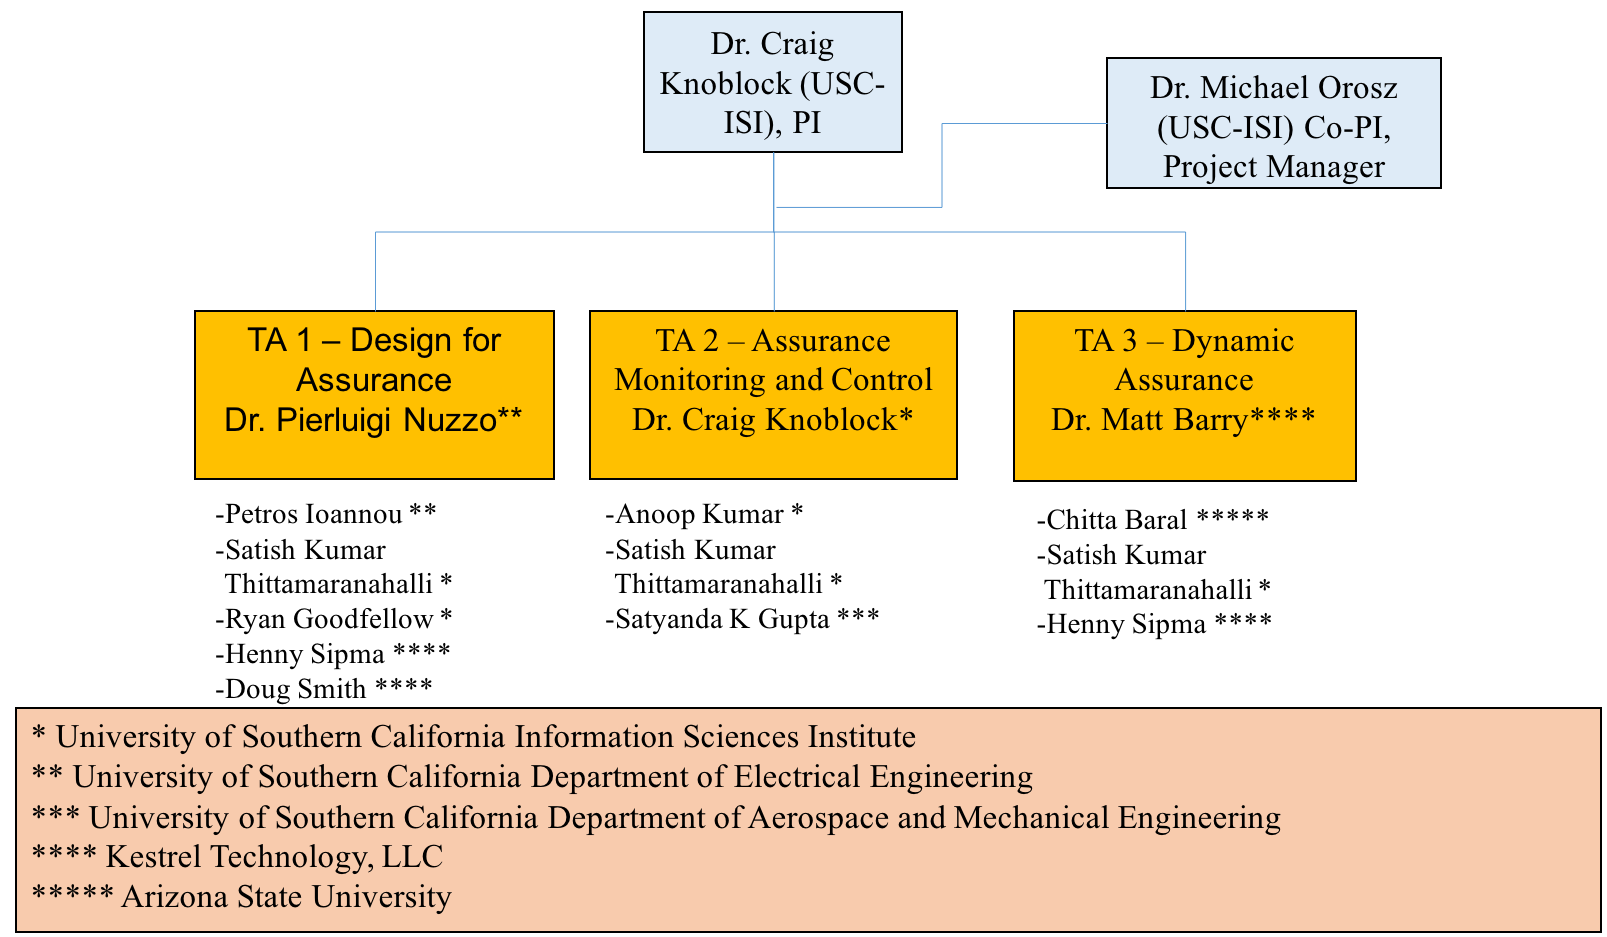
\includegraphics[width=6.0in]{./org-chart2.png}
\caption{\small Organization Chart}
\label{fig:org_chart}
\end{figure}

Coordination: To maximize collaboration and reduce risk to project failure from lack of communication and technical exchange, we plan to employ a wide variety of working styles and communication/coordination so that all can contribute.  At the core of our project will be regularly scheduled meetings bridging the diversely distributed team (Table~\ref{fig:Collaboration_Table}).  These meetings will address project status, identify challenges, implement risk mitigation strategies and participate in technology exchanges and system integration efforts (when appropriate)

\begin{table}[ht]
\caption{\small Project Meetings and Events}
  \centering
  {\footnotesize
\begin{tabular}{|m{3.15in}|m{3in}|} 
\hline
\textbf{Meeting} & \textbf{Frequency} 
\\\hline
Conference calls among investigators (discuss project status, address concerns and project risks) & Weekly
\\
\hline
Technical exchange and coordination meetings using Bluejeans or another videoconference technology & At least twice a month and more frequently as needed
  \\ 
\hline
Face-to-Face meetings (prior to P/I and demonstration meetings) & Every 3 to 6 months and more frequently (especially at the beginning of the project) as needed
 \\\cline{1-2}

\hline
\end{tabular}
}
\label{fig:Collaboration_Table}
\end{table}

\begin{table}[tbhp]
\caption{\small Key Project Team Member Responsibilities}
  \centering
  {\footnotesize
\begin{tabular}{| m{.75in} | m{3.9in}| m{1.5in}|} 
\hline
\textbf{Key Member} & \textbf{Responsibilities} & \textbf{Tasks} 
\\\hline
Dr.\ Craig Knoblock  & Principal Investigator responsible for project, leads TA 2 – Assurance Monitoring and Control.  Will lead the overall project and lead the TA2 team.  Served as the PI on many DARPA projects and has sucessfully led many large teams.    Effort on project:  25\% &
1.1.6, 1.2.2 1.2.3, 1.2.4, 1.3.4, 1.4.1, 
2.1.6, 2.2.2 2.2.3, 2.2.4, 2.3.4, 2.4.1, 
3.1.6, 3.2.2, 3.2.3, 3.2.4, 3.3.4, 3.4.1
\\
\hline
Dr.\ Michael Orosz & Co-Principal Investigator responsible managing the day-to-day operations of the project, assist technical teams as needed, coordinate with TA4 teams.    Has led many large complex multi-disciplined/multi-organizational projects in academic and industry environments.  Effort on project: 50\%
& 1.1.6, 2.1.6, 3.1.6, 1.4.1, 2.4.1, 3.4.1
  \\ 
\hline
Dr.\ Pierluigi Nuzzo 
& 
Co-Principal Investigator.  Leads the TA 1 - Design for Assurance team and conducts research on the formal methods for the design of the TA1 system.  Research experience on methodologies and tools for the design of cyber-physical systems; contracts, interfaces, and compositional methods for embedded system design; the application of automated formal methods and optimization theory to problems in embedded and cyber-physical systems.  Effort on project: 2 months/year (16.6\%)
& 
1.1.1, 2.1.1, 3.1.1 \\
\hline
Dr.\ Matthew Barry
& 
Key personnel.  Leads the TA 3 – Dynamic Assurance.   He will conduct the research on the dynamic assurance case language editors and parsers, the run-time system, and system integrations. Effort on project:  66\%
& 
1.3.2, 2.3.2, 3.3.2\\
\hline
Dr.\ Chitta Baral
& 
Key personnel responsible for learning assurance rules, supporting assurance rules with uncertainty and improving solver speed.  Expertise on ASP solvers, which will be used to reason about the assurance cases. Effort on project: 20\%
& 
1.3.1, 2.3.1, 3.3.1 \\
\hline
Dr.\ Doug Smith 
& 
Key personnel will support formal methods aspects of TA1, and lead the effort on abstract refinement. Expertise in field of automated correct-by-construction program generation.    Effort on project: 40\%
& 
1.1.5, 2.1.5, 3.1.5 \\
\hline
Dr.\ Henny Sipma
& 
Key personnel who will support the program verification tasks under TA1.  Will lead the effort on program verification.   Effort on project:  45\%
& 
1.1.5, 2.1.5, 3.1.5, 1.3.2, 2.3.2, 3.3.2 \\
\hline
Dr.\ Petros Ioannou
& 
Key personnel responsible providing and extending the assurance test bed, which will be available at the start of the project for autonomous vehicles.   Effort on project: 1 month/year (8.3\%)
& 
1.1.2, 2.1.2 (optional), 3.1.2 (optional)
\\
\hline
Dr.\ Satyandra Kumar Gupta
& 
Key Personnel providing autonomous command and control expertise to the TA-2 team.   Will lead the research on safety aware learning on TA2.   Past research on physics-aware decision making to facilitate automation.  Effort on project: 1 month/year (8.3\%)
& 
1.2.1, 2.2.1, 3.2.1 \\
\hline
Dr.\ Anoop Kumar 
& 
Key personnel providing support to the TA 2 project team.  Will lead the research on monitoring \& control and detecting distribution shifts.  Effort on project: 50\%
& 
1.2.1, 1.2.2, 1.2.3, 1.2.4, 2.2.1, 2.2.2, 2.2.3, 2.2.4, 3.2.1, 3.2.2, 3.2.3, 3.2.4\\
\hline
Dr.\ Satish Thittamaranahalli
& 
Key personnel developing scalable algorithms for TA1, TA2, and TA3 project teams.  Has extensive experience on scalable algorithm design, machine learning, and constraint reasoning.  Effort on project: 50\%
& 
1.2.1, 1.2.2, 1.2.3, 1.2.4, 2.2.1, 2.2.2, 2.2.3, 2.2.4, 3.2.1, 3.2.2, 3.2.3, 3.2.4, 1.1.4, 2.1.4, 3.1.4 \\
\hline
Dr.\ Ryan Goodfellow
& 
Key personnel providing support to the TA-1 project. Will lead the research on simulation-based testing.  Has extensive experience on simulation-based testing.  Effort on project:  30\%
& 
1.1.3, 2.1.3, 3.1.3 \\

\cline{1-2}

\hline
\end{tabular}
}
\label{fig:Table_Mgmt}
\end{table}



\newpage
\section{Personnel, Qualifications and Commitment}

{\bf Dr.\ Craig Knoblock}, the PI on this effort, is a Research Professor of both Computer Science and Spatial Sciences at the University of Southern California (USC) and Director of the Intelligent Systems Division at the USC Information Sciences Institute.   He received his Ph.D. from Carnegie Mellon University in computer science. 
%His research focuses on techniques for describing, acquiring, and exploiting the semantics of data.  
In previous projects he has worked on developing  scalable approaches to execution monitoring, accurate detection of sensor failures, and   automatic modeling and reconstruction of sensors.  He has published more than 300 journal articles, book chapters, and conference papers on these topics.  Dr. Knoblock is a Fellow of the Association for the Advancement of Artificial Intelligence (AAAI), a Distinguished Scientist of the Association of Computing Machinery (ACM), a Senior Member of IEEE, past President and Trustee of the International Joint Conference on Artificial Intelligence.
%and winner of the 2014 Robert S. Engelmore Award.  

{\bf Dr.\ Michael Orosz}, a Co-PI on this effort, is a Research Associate Professor of Civil and Environmental Engineering at the University of Southern California (USC) and Research Director of the Decision Systems Group at the USC Information Sciences Institute.  Dr. Orosz has over 30 years’ experience in commercial and government software development, basic and applied research, project management, academic research and has developed and deployed several commercially successful products.  His research interests are in machine learning and decision analytics as applied to intelligence analysis and autonomous command and control such as smart building controls.    Dr. Orosz has extensive experience in managing large complex multi-disciplined/multi-teamed research projects. %funded by DARPA, DHS, DoD, DoE, Industry, NASA, NRO, NSA and ONR.   
He received his Ph.D. in computer science from the University of California, Los Angeles.

{\bf Dr.\ Pierluigi Nuzzo}, a Co-PI on this project, is an Assistant Professor in the Department of Electrical Engineering at the University of Southern California. He received the Ph.D. in Electrical Engineering and Computer Sciences from the University of California at Berkeley. 
%in 2015, and the Laurea degree (MS) in electrical engineering (summa cum laude) from the University of Pisa, Italy, and the Sant'Anna School of Advanced Studies, Pisa, Italy.
%
%He has four years of research experience in analog and mixed signal circuit design as a researcher at IMEC, Leuven, Belgium, and over 10 years experience in design methodologies and tools for mixed-signal integrated circuits and cyber-physical systems, as a researcher at the University of Pisa, IMEC, UC Berkeley, and USC. 
His research interests
include: methodologies and tools for cyber-physical system and mixed-signal
system design; contracts, interfaces and compositional methods for embedded
system design; the application of formal methods and optimization theory to problems in embedded and cyber-physical systems and electronic design automation. 
%
Prof. Nuzzo received %First Place in the operational category and Best Overall
%Submission in the 2006 DAC/ISSCC Design Competition, 
a Marie Curie Fellowship
from the European Union in 2006, 
the University of California at Berkeley EECS
departmental fellowship in 2008, 
%the University of California at Berkeley Outstanding Graduate Student Instructor Award in 2013, 
the IBM Ph.D.
Fellowship in 2012 and 2014, 
%the Best Paper Award from the International Conference on Cyber-Physical Systems (ICCPS) in 2016, 
and the David J.~Sakrison Memorial Prize in 2016 for his doctoral research. 
%He is an author of 1 patent and over 60 publications.

{\bf Dr.\ Satyandra K. Gupta} is Smith International Professor in the Department of Aerospace and Mechanical Engineering at the University of Southern California. %Prior to joining the University of Southern California, he was a Professor in the Department of Mechanical Engineering and the Institute for Systems Research at the University of Maryland. He was the founding director of the Maryland Robotics Center and the Advanced Manufacturing Laboratory at the University of Maryland. 
He served as a program director for the National Robotics Initiative at the National Science Foundation from September 2012 to September 2014.  Dr. Gupta's interest is in the area of physics-aware decision making to facilitate automation. He has published more than 300 technical articles. He is a fellow of the American Society of Mechanical Engineers (ASME) and editor of ASME Journal of Computing and Information Science in Engineering. Dr. Gupta has received the Young Investigator Award from the Office of Naval Research in 2000, CAREER Award from the National Science Foundation in 2001, Presidential Early Career Award for Scientists and Engineers (PECASE) in 2001, Invention of the Year Award at the University of Maryland in 2007, Kos Ishii-Toshiba Award from ASME in 2011, and Excellence in Research Award from ASME in 2013.%, and Distinguished Alumnus Award from Indian Institute of Technology, Roorkee in 2014. %He has also received seven best paper awards at conferences.

{\bf Ryan Goodfellow} is a computer scientist at ISI working in combined cyber physical simulation and emulation platform development. His formal background is in simulation algorithms and modeling techniques using differential-algebraic equations (DAE). He has applied this knowledge in the CPS space by integrating DAE modeling languages and simulation engines with network testbeds to create comprehensive scientific experimentation platforms for cyber-physical systems. These experimentation platforms have been used in the power grid research space. %Ryan is a lead developer on the Deter network testbed, with a strong background in networked and distributed systems engineering. %He is also a combat veteran, serving as a non-commissioned officer and SIGINT team lead for a multi-functional intelligence team in Afghanistan.

{\bf Dr.\ Petros Ioannou} is a Professor in the Department of Electrical Engineering, Director of the Center for Advanced Transportation Technologies and Associate Director for Research for the DOT supported University Transportation Center at USC. He received his MS and PhD from the University of Illinois at Urbana Champaign in Mechanical and Electrical Engineering, respectively. His research interests are in robust adaptive control, vehicle dynamics and control, human factors and safety, automated vehicles, nonlinear systems and Intelligent transportation Systems.  He received the 2016 IEEE Transportation Technologies field award and the 2016 IEEE Control system society Transition to Practice Award. He is a Fellow of IEEE, IFAC and IET and author/coauthor of 8 books and over 400 papers.

{\bf Dr.\ Matthew Barry} will serve as lead for the TA3 tasks. %He will implement the dynamic assurance case language editors and parsers, the run-time system, and system integrations.  He will implement the assurance case arguments and the API for updating argument structure and content.  
Dr. Barry currently is CEO at Kestrel Technology LLC, and previously spent 20 years in NASA space mission operations at the Jet Propulsion Lab and Johnson Space Center.  At NASA Headquarters he led the introduction of dependability case requirements and plans for flight computing systems in upcoming manned space exploration missions, as well as the development of Agency-level software-related safety-critical control system requirements.  He recently served as a Principal Investigator on DHS/Cyber S\&T STAMP (Static Tool Analysis Modernization Program), DARPA CSFV (Crowd Sourced Formal Verification), three NASA Aeronautics R\&D projects, and the AFRL-sponsored Static Analysis of Numerical Algorithms project.  Dr. Barry earned BSME, MS, and PhD degrees in mechanical engineering, and an MBA degree, from Rice University.  

{\bf Dr.\ Henny Sipma} will support the program verification tasks under TA1.  %She is the key person behind the company's {\em KT Advance\/} and {\em KT Transferal\/} static analysis products, and the designer and programmer of the company's core {\em CodeHawk\/} abstract interpretation engine. 
Dr. Sipma currently is the CTO at Kestrel Technology LLC.  She has spent the past 10 years with Kestrel Technology as a static analysis expert; previously developed and taught static analysis techniques as senior research associate at Stanford University for eight years; and developed industrial process controls as an senior systems analyst at Shell.  She has been Principal Investigator or company lead on several recent R\&D projects for Federal agencies, including two projects under the IARPA STONESOUP (Securely Taking On New Executable Software of Uncertain Provenance) program; the DHS Cyber S\&T Gold Standard project; and the DARPA-sponsored STAC (Space-Time Analysis for Cybersecurity) and MUSE (Mining and Understanding Software Enclaves) programs.  Dr. Sipma earned 
%a BS degree in chemistry and an MS degree in chemical engineering at the University of Groningen in The Netherlands, and 
MS and PhD degrees in computer science from Stanford University.  

{\bf Dr.\ Douglas R.\ Smith} will support formal methods aspects of TA1, including the enforcement of safety properties and the generation of monitors.  He is President of Kestrel Technology LLC and Principal Scientist at Kestrel Institute.  He is a Fellow of the American Association of Artificial Intelligence (AAAI) and an ASE Fellow (Automated Software Engineering).  From 1986 to 2000, he taught an advanced graduate course on correct-by-construction software development at Stanford.  
%Dr. Smith has led the development of a series of software synthesis systems, including KIDS (Kestrel Interactive Development System), Specware, Designware, and Planware. 
%Applications domains have included a variety of complex high-performance planners and schedulers for the US Air Force.  He leads current projects on the generation of air mission plans and cyberoperations.  
Other recent projects focused on automated policy enforcement \cite{SmithD0703,SmithD08}, synthesis of secure network protocol codes, and the synthesis of high-performance constraint-solvers\cite{SmithD08c,SmithD13}.  Dr. Smith has over 30 years experience in the field of automated correct-by-construction program generation and has published over 100 papers. He has one patent.  He received the Ph.D. in Computer Science from Duke University% in 1979.  

{\bf Dr. Chitta Baral} is a Professor in the Department of Computer Science and Engineering at Arizona State University. He will support the TA3 efforts on Learning assurance rules, supporting assurance rules with uncertainty and improving solver speed. Dr. Baral has expertise in various aspects of autonomy and Artificial Intelligence. 
He wrote the first book on answer set programming (published by Cambridge University Press) the formal language behind our assurance rules. Some of his other works relevant to this proposal are: goal specification for autonomous systems, automatic construction of control rules for autonomous systems that satisfy given goals, combining machine learning with reasoning in various contexts, including image understanding. %He is the President of KR Inc. He is an associate editor of AIJ and has been an associate editor of JAIR.

{\bf Dr.\ Satish Kumar Thittamaranahalli (T. K. Satish Kumar)} leads the Collaboratory for Algorithmic Techniques and Artificial Intelligence (CATAI) at USC's Information Sciences Institute. He has published over 60 papers on numerous topics in Artificial Intelligence spanning such diverse areas as Constraint Reasoning, Planning and Scheduling, Probabilistic Reasoning, Robotics, Combinatorial Optimization, Approximation and Randomization, Heuristic Search, Model-Based Reasoning, Knowledge Representation and Spatio-Temporal Reasoning. %He %has served on the Program Committees of many international conferences in Artificial Intelligence
He and is a winner of the 2016 Best Robotics Paper Award and the 2005 Best Student Paper Award from the International Conference on Automated Planning and Scheduling. 
Dr. Kumar received his PhD in Computer Science from Stanford University. %In the past, he has also been a Visiting Student at the NASA Ames Research Center, a Postdoctoral Research Scholar at the University of California, Berkeley, a Research Scientist at the Institute for Human and Machine Cognition, a Visiting Assistant Professor at the University of West Florida, and a Senior Research and Development Scientist at Mission Critical Technologies.

\textbf{Dr.\ Anoop Kumar} is a senior computer scientist at USC ISI and has broad expertise in machine learning, statistical modeling, and software engineering.  Dr.\ Kumar is the technical lead on the DARPA RSPACE program and has played a vital role in developing a system that fuses air operations data from multiple sources, maintains world state, and issues warnings. Previously, he led the research and development of the BBN’s election forecasting system for the IARPA OSI program. %Dr.\ Kumar played a significant role in the DARPA DEFT program by developing a model to support integration of output from multiple NLP algorithms. He has contributed at the development to management levels on government research contracts and commercial projects. 
Dr.\ Kumar helped design and develop BBN's commercially available, hosted speech and medical transcription services offering. 

\begin{table}[!tbh]
\begin{footnotesize}
\vspace{-0.1in}

\begin{tabular}{lll}
\begin{tabular}[t]{|l|@{}c@{}|@{}c@{}|@{}c@{}|@{}c@{}|} \hline
Project & Status & \multicolumn{3}{ c| }{Hours} \\ \cline{3-5}
& & P1 & P2 & P3 \\ \hline



\multicolumn{5}{ |c| }{ \textbf{Craig Knoblock} } \\ \cline{1-5}
Safeguard & Pro & 770 & 641 & 641 \\ \cline{1-5}
ELICIT & Cur & 308 & 256 & 120 \\ \cline{1-5}
WTNIC & Cur & 11 & 0 & 0 \\ \cline{1-5}
EFFECT & Cur & 641 & 107 & 0 \\ \cline{1-5}
LinkedMaps & Cur & 203 & 25 & 0 \\ \cline{1-5}
PRINCESS & Cur & 608 & 96 & 0 \\ \cline{1-5}
SCHARP & Cur & 481 & 54 & 0 \\ \cline{1-5}
MINT & Pen & 650 & 534 & 285 \\ \cline{1-5}

\multicolumn{5}{ |c| }{ \textbf{Michael Orosz} } \\ \cline{1-5}
Safeguard & Pro & 1560 & 1300 & 1300  \\ \cline{1-5}
SMC/SY & Cur & 1803 & 0 & 0  \\ \cline{1-5}

\multicolumn{5}{ |c| }{ \textbf{Matthew Barry} } \\ \cline{1-5}
Safeguard & Pro & 2078 & 1690 & 1554 \\ \cline{1-5}
Starlite & Cur & 1840 & 1692 & 0 \\ \cline{1-5}



\multicolumn{5}{ |c| }{ \textbf{Anoop Kumar} } \\ \cline{1-5}
Safeguard & Pro & 1560 & 1300 & 1300 \\ \cline{1-5}

\end{tabular}
&
\begin{tabular}[t]{|l|@{}c@{}|@{}c@{}|@{}c@{}|@{}c@{}|} \hline
Project & Status & \multicolumn{3}{ c| }{Hours} \\ \cline{3-5}
& & P1 & P2 & P3 \\ \hline

\multicolumn{5}{ |c| }{ \textbf{Pierluigi Nuzzo} } \\ \cline{1-5}
Safeguard & Pro & 520 & 433 & 433  \\ \cline{1-5}
Mirage & Cur & 433 & 0 & 0  \\ \cline{1-5}

\multicolumn{5}{ |c| }{ \textbf{Satyandra Gupta} } \\ \cline{1-5}
Safeguard & Pro & 260 & 217 & 217 \\ \cline{1-5}
Human   & Cur & 22 & 0 & 0 \\ \cline{1-5}
Vehicles & Cur & 36 & 0 & 0 \\ \cline{1-5}
Robot & Cur & 116 & 0 & 0 \\ \cline{1-5}
Assembly & Cur & 33 & 0 & 0 \\ \cline{1-5}
Solar & Cur & 4 & 0 & 0 \\ \cline{1-5}

\multicolumn{5}{ |c| }{ \textbf{Petros Ioannou} } \\ \cline{1-5}
Safeguard & Pro & 260 & 217 & 217 \\ \cline{1-5}
CPS & Cur & 130 & 0 & 0 \\ \cline{1-5}

\multicolumn{5}{ |c| }{ \textbf{Ryan Goodfellow} } \\ \cline{1-5}
Safeguard & Pro & 936 & 780 & 780 \\ \cline{1-5}
STEAM & Cur & 416 & 0 & 0 \\ \cline{1-5}


\end{tabular}
&
\begin{tabular}[t]{|l|@{}c@{}|@{}c@{}|@{}c@{}|@{}c@{}|} \hline
Project & Status & \multicolumn{3}{ c| }{Hours} \\ \cline{3-5}
& & P1 & P2 & P3 \\ \hline

\multicolumn{5}{ |c| }{ \textbf{Chitta Baral} } \\ \cline{1-5}
Safeguard & Pro & 659 & 485 & 485 \\ \cline{1-5}
PostdocBP & Cur & 176 & 0 & 0 \\ \cline{1-5}
Languages & Pen & 528 & 264 & 264 \\ \cline{1-5}
CAREER & Pen & 88 & 44 & 44 \\ \cline{1-5}
CHS & Pen & 510 & 255 & 0 \\ \cline{1-5}

\multicolumn{5}{ |c| }{ \textbf{Doug Smith} } \\ \cline{1-5}
Safeguard & Pro & 1222 & 984 & 840 \\ \cline{1-5}
RSPACE & Cur & 342 & 0 & 0 \\ 
\cline{1-5}
PLANX & Cur & 154 & 0 & 0 \\ 
\cline{1-5}
HACCS & Pen & 923 & 769 & 769 \\ 
\cline{1-5}

\multicolumn{5}{ |c| }{ \textbf{Henny Sipma} } \\ \cline{1-5}
Safeguard & Pro & 1372 & 962 & 840 \\ \cline{1-5}
STAC & Cur & 797 & 0 & 0 \\ \cline{1-5}

\multicolumn{5}{ |c| }{ \textbf{Satish Thittamaranahalli} } \\ \cline{1-5}
Safeguard & Pro & 1560 & 1300 & 1300 \\ \cline{1-5}
MapF & Cur & 103 & 103 & 0 \\ \cline{1-5}

\end{tabular}
\end{tabular}

\end{footnotesize}
\caption{Individual commitments of key personnel}
\label{tab:Commitments}
\vspace{-0.2in}
\end{table}

\clearpage
\newpage
\section{Capabilities}


%\subsection{University of Southern California}
USC has strengths in number of areas that are closely related to the proposed work:
\begin{itemize}[itemsep=0pt,leftmargin=*]
\item Dr.\ Nuzzo 
%has over 10-year research experience in embedded system design, from mixed-signal chip design (analog-to-digital converters, frequency synthesizers, software-defined radio), to methodologies and tools for mixed-signal integrated circuits and Cyber-Physical Systems (CPSs), and the application of formal methods and optimization theory to problems in embedded and cyber-physical systems and electronic design automation.  
%His doctoral work 
has done extensive research on contracts and compositional methods for heterogeneous system design and design space exploration, with application to aircraft electric power systems and environmental control systems. His work has helped transition rigorous system design foundations, innovative design methodologies, and new systems engineering paradigms to industry (IBM, United Technologies). 
\item Dr.\ Satyandra K. Gupta has worked on autonomous surface vehicles, autonomous ground vehicles for operation on rugged terrains, and autonomous flapping wing aerial vehicles.   His group has developed a hierarchal decision making approach for realizing autonomous systems. 
%This approach combines task planning and assignment, deliberative trajectory planning, reactive collision avoidance behaviors, and trajectory tracking control layers. 
His group has also developed new methods for learning reactive behaviors in adversarial environments and COLREGS compliant trajectory planning. \item Dr.\ Knoblock has developed methods that learn the relationships between sensors to both identify failures and changes in sensor and reconstruct those sensors, providing estimates of the accuracy of the reconstructed sensors.  
\item Ryan Goodfellow has extensive experience in simulation based testing through high-fidelity CPS testbed environment development and operation, using the Deter network testbed as the core which has supported several large scale government projects from a variety of agencies and thousands of users. %we have developed sophisticated CPS experiments under programs such as NFS RIPS, NIST SmartCities and the DHS Cybersecurity showcase.
\item Dr.\ Ioannou %helped  design and implement adaptive cruise control systems in collaboration with Ford Motor Company, which was commercialized four years before any other company. He 
worked on several DOT funded projects on automated vehicles and intelligent highway systems where he demonstrated his vehicle control designs for safety and performance on actual automated vehicles in test trucks and I-15 highway.
\item Drs.\ Knoblock, Kumar, and Thittamaranahalli have developed highly scalable approaches for monitoring message traffic to identify potential problems and issue warnings and alerts. 
\item Dr. Thittamaranahalli has developed state-of-the-art methods for efficiently solving large-scale search and optimization problems. %These techniques will be applicable in TA2 for safety-aware learning and planning, in TA2 for assurance monitoring and control, and in TA3 for dynamic assessment of assurance cases.

\end{itemize}
%\subsection{Kestrel Technology LLC}

Kestrel Technology's strength is in program analysis, specifically static analysis of both source and binary targets.  The company performs applied R\&D and product development for a variety of static analysis applications  pivoting primarily on the abstract interpretation technique.  The company recently initiated development of program analysis applications using logical equivalence techniques. As a provider of verification evidence in the form of mathematical proofs, the company also has expertise in the design and development of assurance case arguments for high-integrity systems using such evidence. %The company is engaged in a partnership with Wind River Systems to develop program analysis tools for its embedded system developers.  Many of Wind River's customers must develop their products under safety and certification standards, including those using safety cases.  

   

%\subsection{Arizona State University}
Chitta Baral at Arizona State University has developed various software to learn assurance rules and various ASP solvers, which he has made available as open-source.

Most of the software carried forward for implementation or derivation is open source.  The single exception is Kestrel Technology's {\it KT Advance\/} static analysis tool (TA1), in particular the abstract interpretation engine therein, which is company proprietary and is US EAR export-controlled.   
%Owing to mixed funding for the development of that technology 
We will continue to provide the Federal government a restricted use license for that particular item.

There are no specialized facilities, data, or GFE required for this effort. 

\include{sow}
\include{milestones}

% \section{Level of Effort by Task \textcolor{red}{[Mike/Lisa - 1 pages]}}

% \textcolor{blue}{
% \begin{itemize}
% \item Will be a separate spreadsheet
% \item
% \end{itemize}
% }

\include{appendix_a}

%\section{Appendix B \textcolor{red}{[No Page Count]}}

\section{References}
\bibliographystyle{acm} 
\bibliography{TA3/ta3,TA2/ta2,TA1/ta1}
\end{document}
\clearpage
\newpage


\section{Management Plan}


The Principal Investigator for this effort is Dr. Craig Knoblock who is responsible for all aspects of the effort, will coordinate the parallel team efforts, and will ensure high levels of performance from individual team members.  The Co-P/I, Dr. Michael Orosz, will provide project management and will assist all performers in the execution of the project.    The project team is divided into three working groups (Figure~\ref{fig:org_chart}) corresponding to Technical Areas 1-3, however, members of each team contribute across all project activities.   Table~\ref{fig:Table_Mgmt} defines the major contributions of each project team member to the project tasks.

\begin{figure}[tbhp]
%\vspace{-25pt}
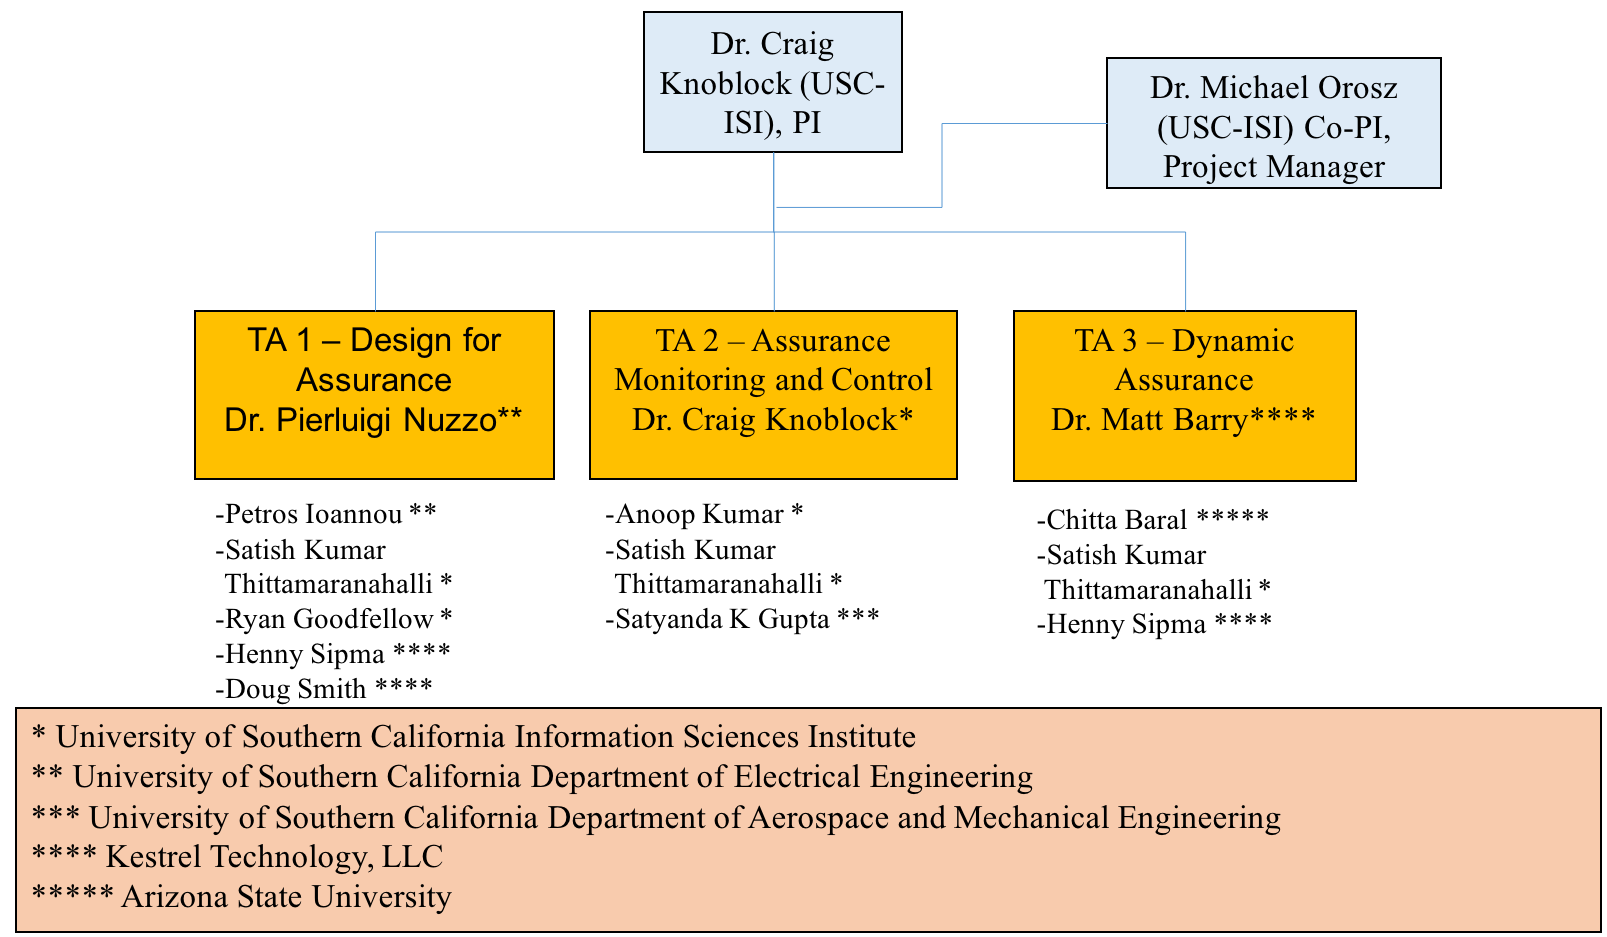
\includegraphics[width=6.0in]{./org-chart2.png}
\caption{\small Organization Chart}
\label{fig:org_chart}
\end{figure}

Coordination: To maximize collaboration and reduce risk to project failure from lack of communication and technical exchange, we plan to employ a wide variety of working styles and communication/coordination so that all can contribute.  At the core of our project will be regularly scheduled meetings bridging the diversely distributed team (Table~\ref{fig:Collaboration_Table}).  These meetings will address project status, identify challenges, implement risk mitigation strategies and participate in technology exchanges and system integration efforts (when appropriate)

\begin{table}[ht]
\caption{\small Project Meetings and Events}
  \centering
  {\footnotesize
\begin{tabular}{|m{3.15in}|m{3in}|} 
\hline
\textbf{Meeting} & \textbf{Frequency} 
\\\hline
Conference calls among investigators (discuss project status, address concerns and project risks) & Weekly
\\
\hline
Technical exchange and coordination meetings using Bluejeans or another videoconference technology & At least twice a month and more frequently as needed
  \\ 
\hline
Face-to-Face meetings (prior to P/I and demonstration meetings) & Every 3 to 6 months and more frequently (especially at the beginning of the project) as needed
 \\\cline{1-2}

\hline
\end{tabular}
}
\label{fig:Collaboration_Table}
\end{table}

\begin{table}[tbhp]
\caption{\small Key Project Team Member Responsibilities}
  \centering
  {\footnotesize
\begin{tabular}{| m{.75in} | m{3.9in}| m{1.5in}|} 
\hline
\textbf{Key Member} & \textbf{Responsibilities} & \textbf{Tasks} 
\\\hline
Dr.\ Craig Knoblock  & Principal Investigator responsible for project, leads TA 2 – Assurance Monitoring and Control.  Will lead the overall project and lead the TA2 team.  Served as the PI on many DARPA projects and has sucessfully led many large teams.    Effort on project:  25\% &
1.1.6, 1.2.2 1.2.3, 1.2.4, 1.3.4, 1.4.1, 
2.1.6, 2.2.2 2.2.3, 2.2.4, 2.3.4, 2.4.1, 
3.1.6, 3.2.2, 3.2.3, 3.2.4, 3.3.4, 3.4.1
\\
\hline
Dr.\ Michael Orosz & Co-Principal Investigator responsible managing the day-to-day operations of the project, assist technical teams as needed, coordinate with TA4 teams.    Has led many large complex multi-disciplined/multi-organizational projects in academic and industry environments.  Effort on project: 50\%
& 1.1.6, 2.1.6, 3.1.6, 1.4.1, 2.4.1, 3.4.1
  \\ 
\hline
Dr.\ Pierluigi Nuzzo 
& 
Co-Principal Investigator.  Leads the TA 1 - Design for Assurance team and conducts research on the formal methods for the design of the TA1 system.  Research experience on methodologies and tools for the design of cyber-physical systems; contracts, interfaces, and compositional methods for embedded system design; the application of automated formal methods and optimization theory to problems in embedded and cyber-physical systems.  Effort on project: 2 months/year (16.6\%)
& 
1.1.1, 2.1.1, 3.1.1 \\
\hline
Dr.\ Matthew Barry
& 
Key personnel.  Leads the TA 3 – Dynamic Assurance.   He will conduct the research on the dynamic assurance case language editors and parsers, the run-time system, and system integrations. Effort on project:  66\%
& 
1.3.2, 2.3.2, 3.3.2\\
\hline
Dr.\ Chitta Baral
& 
Key personnel responsible for learning assurance rules, supporting assurance rules with uncertainty and improving solver speed.  Expertise on ASP solvers, which will be used to reason about the assurance cases. Effort on project: 20\%
& 
1.3.1, 2.3.1, 3.3.1 \\
\hline
Dr.\ Doug Smith 
& 
Key personnel will support formal methods aspects of TA1, and lead the effort on abstract refinement. Expertise in field of automated correct-by-construction program generation.    Effort on project: 40\%
& 
1.1.5, 2.1.5, 3.1.5 \\
\hline
Dr.\ Henny Sipma
& 
Key personnel who will support the program verification tasks under TA1.  Will lead the effort on program verification.   Effort on project:  45\%
& 
1.1.5, 2.1.5, 3.1.5, 1.3.2, 2.3.2, 3.3.2 \\
\hline
Dr.\ Petros Ioannou
& 
Key personnel responsible providing and extending the assurance test bed, which will be available at the start of the project for autonomous vehicles.   Effort on project: 1 month/year (8.3\%)
& 
1.1.2, 2.1.2 (optional), 3.1.2 (optional)
\\
\hline
Dr.\ Satyandra Kumar Gupta
& 
Key Personnel providing autonomous command and control expertise to the TA-2 team.   Will lead the research on safety aware learning on TA2.   Past research on physics-aware decision making to facilitate automation.  Effort on project: 1 month/year (8.3\%)
& 
1.2.1, 2.2.1, 3.2.1 \\
\hline
Dr.\ Anoop Kumar 
& 
Key personnel providing support to the TA 2 project team.  Will lead the research on monitoring \& control and detecting distribution shifts.  Effort on project: 50\%
& 
1.2.1, 1.2.2, 1.2.3, 1.2.4, 2.2.1, 2.2.2, 2.2.3, 2.2.4, 3.2.1, 3.2.2, 3.2.3, 3.2.4\\
\hline
Dr.\ Satish Thittamaranahalli
& 
Key personnel developing scalable algorithms for TA1, TA2, and TA3 project teams.  Has extensive experience on scalable algorithm design, machine learning, and constraint reasoning.  Effort on project: 50\%
& 
1.2.1, 1.2.2, 1.2.3, 1.2.4, 2.2.1, 2.2.2, 2.2.3, 2.2.4, 3.2.1, 3.2.2, 3.2.3, 3.2.4, 1.1.4, 2.1.4, 3.1.4 \\
\hline
Dr.\ Ryan Goodfellow
& 
Key personnel providing support to the TA-1 project. Will lead the research on simulation-based testing.  Has extensive experience on simulation-based testing.  Effort on project:  30\%
& 
1.1.3, 2.1.3, 3.1.3 \\

\cline{1-2}

\hline
\end{tabular}
}
\label{fig:Table_Mgmt}
\end{table}



\newpage
\section{Personnel, Qualifications and Commitment}

{\bf Dr.\ Craig Knoblock}, the PI on this effort, is a Research Professor of both Computer Science and Spatial Sciences at the University of Southern California (USC) and Director of the Intelligent Systems Division at the USC Information Sciences Institute.   He received his Ph.D. from Carnegie Mellon University in computer science. 
%His research focuses on techniques for describing, acquiring, and exploiting the semantics of data.  
In previous projects he has worked on developing  scalable approaches to execution monitoring, accurate detection of sensor failures, and   automatic modeling and reconstruction of sensors.  He has published more than 300 journal articles, book chapters, and conference papers on these topics.  Dr. Knoblock is a Fellow of the Association for the Advancement of Artificial Intelligence (AAAI), a Distinguished Scientist of the Association of Computing Machinery (ACM), a Senior Member of IEEE, past President and Trustee of the International Joint Conference on Artificial Intelligence.
%and winner of the 2014 Robert S. Engelmore Award.  

{\bf Dr.\ Michael Orosz}, a Co-PI on this effort, is a Research Associate Professor of Civil and Environmental Engineering at the University of Southern California (USC) and Research Director of the Decision Systems Group at the USC Information Sciences Institute.  Dr. Orosz has over 30 years’ experience in commercial and government software development, basic and applied research, project management, academic research and has developed and deployed several commercially successful products.  His research interests are in machine learning and decision analytics as applied to intelligence analysis and autonomous command and control such as smart building controls.    Dr. Orosz has extensive experience in managing large complex multi-disciplined/multi-teamed research projects. %funded by DARPA, DHS, DoD, DoE, Industry, NASA, NRO, NSA and ONR.   
He received his Ph.D. in computer science from the University of California, Los Angeles.

{\bf Dr.\ Pierluigi Nuzzo}, a Co-PI on this project, is an Assistant Professor in the Department of Electrical Engineering at the University of Southern California. He received the Ph.D. in Electrical Engineering and Computer Sciences from the University of California at Berkeley. 
%in 2015, and the Laurea degree (MS) in electrical engineering (summa cum laude) from the University of Pisa, Italy, and the Sant'Anna School of Advanced Studies, Pisa, Italy.
%
%He has four years of research experience in analog and mixed signal circuit design as a researcher at IMEC, Leuven, Belgium, and over 10 years experience in design methodologies and tools for mixed-signal integrated circuits and cyber-physical systems, as a researcher at the University of Pisa, IMEC, UC Berkeley, and USC. 
His research interests
include: methodologies and tools for cyber-physical system and mixed-signal
system design; contracts, interfaces and compositional methods for embedded
system design; the application of formal methods and optimization theory to problems in embedded and cyber-physical systems and electronic design automation. 
%
Prof. Nuzzo received %First Place in the operational category and Best Overall
%Submission in the 2006 DAC/ISSCC Design Competition, 
a Marie Curie Fellowship
from the European Union in 2006, 
the University of California at Berkeley EECS
departmental fellowship in 2008, 
%the University of California at Berkeley Outstanding Graduate Student Instructor Award in 2013, 
the IBM Ph.D.
Fellowship in 2012 and 2014, 
%the Best Paper Award from the International Conference on Cyber-Physical Systems (ICCPS) in 2016, 
and the David J.~Sakrison Memorial Prize in 2016 for his doctoral research. 
%He is an author of 1 patent and over 60 publications.

{\bf Dr.\ Satyandra K. Gupta} is Smith International Professor in the Department of Aerospace and Mechanical Engineering at the University of Southern California. %Prior to joining the University of Southern California, he was a Professor in the Department of Mechanical Engineering and the Institute for Systems Research at the University of Maryland. He was the founding director of the Maryland Robotics Center and the Advanced Manufacturing Laboratory at the University of Maryland. 
He served as a program director for the National Robotics Initiative at the National Science Foundation from September 2012 to September 2014.  Dr. Gupta's interest is in the area of physics-aware decision making to facilitate automation. He has published more than 300 technical articles. He is a fellow of the American Society of Mechanical Engineers (ASME) and editor of ASME Journal of Computing and Information Science in Engineering. Dr. Gupta has received the Young Investigator Award from the Office of Naval Research in 2000, CAREER Award from the National Science Foundation in 2001, Presidential Early Career Award for Scientists and Engineers (PECASE) in 2001, Invention of the Year Award at the University of Maryland in 2007, Kos Ishii-Toshiba Award from ASME in 2011, and Excellence in Research Award from ASME in 2013.%, and Distinguished Alumnus Award from Indian Institute of Technology, Roorkee in 2014. %He has also received seven best paper awards at conferences.

{\bf Ryan Goodfellow} is a computer scientist at ISI working in combined cyber physical simulation and emulation platform development. His formal background is in simulation algorithms and modeling techniques using differential-algebraic equations (DAE). He has applied this knowledge in the CPS space by integrating DAE modeling languages and simulation engines with network testbeds to create comprehensive scientific experimentation platforms for cyber-physical systems. These experimentation platforms have been used in the power grid research space. %Ryan is a lead developer on the Deter network testbed, with a strong background in networked and distributed systems engineering. %He is also a combat veteran, serving as a non-commissioned officer and SIGINT team lead for a multi-functional intelligence team in Afghanistan.

{\bf Dr.\ Petros Ioannou} is a Professor in the Department of Electrical Engineering, Director of the Center for Advanced Transportation Technologies and Associate Director for Research for the DOT supported University Transportation Center at USC. He received his MS and PhD from the University of Illinois at Urbana Champaign in Mechanical and Electrical Engineering, respectively. His research interests are in robust adaptive control, vehicle dynamics and control, human factors and safety, automated vehicles, nonlinear systems and Intelligent transportation Systems.  He received the 2016 IEEE Transportation Technologies field award and the 2016 IEEE Control system society Transition to Practice Award. He is a Fellow of IEEE, IFAC and IET and author/coauthor of 8 books and over 400 papers.

{\bf Dr.\ Matthew Barry} will serve as lead for the TA3 tasks. %He will implement the dynamic assurance case language editors and parsers, the run-time system, and system integrations.  He will implement the assurance case arguments and the API for updating argument structure and content.  
Dr. Barry currently is CEO at Kestrel Technology LLC, and previously spent 20 years in NASA space mission operations at the Jet Propulsion Lab and Johnson Space Center.  At NASA Headquarters he led the introduction of dependability case requirements and plans for flight computing systems in upcoming manned space exploration missions, as well as the development of Agency-level software-related safety-critical control system requirements.  He recently served as a Principal Investigator on DHS/Cyber S\&T STAMP (Static Tool Analysis Modernization Program), DARPA CSFV (Crowd Sourced Formal Verification), three NASA Aeronautics R\&D projects, and the AFRL-sponsored Static Analysis of Numerical Algorithms project.  Dr. Barry earned BSME, MS, and PhD degrees in mechanical engineering, and an MBA degree, from Rice University.  

{\bf Dr.\ Henny Sipma} will support the program verification tasks under TA1.  %She is the key person behind the company's {\em KT Advance\/} and {\em KT Transferal\/} static analysis products, and the designer and programmer of the company's core {\em CodeHawk\/} abstract interpretation engine. 
Dr. Sipma currently is the CTO at Kestrel Technology LLC.  She has spent the past 10 years with Kestrel Technology as a static analysis expert; previously developed and taught static analysis techniques as senior research associate at Stanford University for eight years; and developed industrial process controls as an senior systems analyst at Shell.  She has been Principal Investigator or company lead on several recent R\&D projects for Federal agencies, including two projects under the IARPA STONESOUP (Securely Taking On New Executable Software of Uncertain Provenance) program; the DHS Cyber S\&T Gold Standard project; and the DARPA-sponsored STAC (Space-Time Analysis for Cybersecurity) and MUSE (Mining and Understanding Software Enclaves) programs.  Dr. Sipma earned 
%a BS degree in chemistry and an MS degree in chemical engineering at the University of Groningen in The Netherlands, and 
MS and PhD degrees in computer science from Stanford University.  

{\bf Dr.\ Douglas R.\ Smith} will support formal methods aspects of TA1, including the enforcement of safety properties and the generation of monitors.  He is President of Kestrel Technology LLC and Principal Scientist at Kestrel Institute.  He is a Fellow of the American Association of Artificial Intelligence (AAAI) and an ASE Fellow (Automated Software Engineering).  From 1986 to 2000, he taught an advanced graduate course on correct-by-construction software development at Stanford.  
%Dr. Smith has led the development of a series of software synthesis systems, including KIDS (Kestrel Interactive Development System), Specware, Designware, and Planware. 
%Applications domains have included a variety of complex high-performance planners and schedulers for the US Air Force.  He leads current projects on the generation of air mission plans and cyberoperations.  
Other recent projects focused on automated policy enforcement \cite{SmithD0703,SmithD08}, synthesis of secure network protocol codes, and the synthesis of high-performance constraint-solvers\cite{SmithD08c,SmithD13}.  Dr. Smith has over 30 years experience in the field of automated correct-by-construction program generation and has published over 100 papers. He has one patent.  He received the Ph.D. in Computer Science from Duke University% in 1979.  

{\bf Dr. Chitta Baral} is a Professor in the Department of Computer Science and Engineering at Arizona State University. He will support the TA3 efforts on Learning assurance rules, supporting assurance rules with uncertainty and improving solver speed. Dr. Baral has expertise in various aspects of autonomy and Artificial Intelligence. 
He wrote the first book on answer set programming (published by Cambridge University Press) the formal language behind our assurance rules. Some of his other works relevant to this proposal are: goal specification for autonomous systems, automatic construction of control rules for autonomous systems that satisfy given goals, combining machine learning with reasoning in various contexts, including image understanding. %He is the President of KR Inc. He is an associate editor of AIJ and has been an associate editor of JAIR.

{\bf Dr.\ Satish Kumar Thittamaranahalli (T. K. Satish Kumar)} leads the Collaboratory for Algorithmic Techniques and Artificial Intelligence (CATAI) at USC's Information Sciences Institute. He has published over 60 papers on numerous topics in Artificial Intelligence spanning such diverse areas as Constraint Reasoning, Planning and Scheduling, Probabilistic Reasoning, Robotics, Combinatorial Optimization, Approximation and Randomization, Heuristic Search, Model-Based Reasoning, Knowledge Representation and Spatio-Temporal Reasoning. %He %has served on the Program Committees of many international conferences in Artificial Intelligence
He and is a winner of the 2016 Best Robotics Paper Award and the 2005 Best Student Paper Award from the International Conference on Automated Planning and Scheduling. 
Dr. Kumar received his PhD in Computer Science from Stanford University. %In the past, he has also been a Visiting Student at the NASA Ames Research Center, a Postdoctoral Research Scholar at the University of California, Berkeley, a Research Scientist at the Institute for Human and Machine Cognition, a Visiting Assistant Professor at the University of West Florida, and a Senior Research and Development Scientist at Mission Critical Technologies.

\textbf{Dr.\ Anoop Kumar} is a senior computer scientist at USC ISI and has broad expertise in machine learning, statistical modeling, and software engineering.  Dr.\ Kumar is the technical lead on the DARPA RSPACE program and has played a vital role in developing a system that fuses air operations data from multiple sources, maintains world state, and issues warnings. Previously, he led the research and development of the BBN’s election forecasting system for the IARPA OSI program. %Dr.\ Kumar played a significant role in the DARPA DEFT program by developing a model to support integration of output from multiple NLP algorithms. He has contributed at the development to management levels on government research contracts and commercial projects. 
Dr.\ Kumar helped design and develop BBN's commercially available, hosted speech and medical transcription services offering. 

\begin{table}[!tbh]
\begin{footnotesize}
\vspace{-0.1in}

\begin{tabular}{lll}
\begin{tabular}[t]{|l|@{}c@{}|@{}c@{}|@{}c@{}|@{}c@{}|} \hline
Project & Status & \multicolumn{3}{ c| }{Hours} \\ \cline{3-5}
& & P1 & P2 & P3 \\ \hline



\multicolumn{5}{ |c| }{ \textbf{Craig Knoblock} } \\ \cline{1-5}
Safeguard & Pro & 770 & 641 & 641 \\ \cline{1-5}
ELICIT & Cur & 308 & 256 & 120 \\ \cline{1-5}
WTNIC & Cur & 11 & 0 & 0 \\ \cline{1-5}
EFFECT & Cur & 641 & 107 & 0 \\ \cline{1-5}
LinkedMaps & Cur & 203 & 25 & 0 \\ \cline{1-5}
PRINCESS & Cur & 608 & 96 & 0 \\ \cline{1-5}
SCHARP & Cur & 481 & 54 & 0 \\ \cline{1-5}
MINT & Pen & 650 & 534 & 285 \\ \cline{1-5}

\multicolumn{5}{ |c| }{ \textbf{Michael Orosz} } \\ \cline{1-5}
Safeguard & Pro & 1560 & 1300 & 1300  \\ \cline{1-5}
SMC/SY & Cur & 1803 & 0 & 0  \\ \cline{1-5}

\multicolumn{5}{ |c| }{ \textbf{Matthew Barry} } \\ \cline{1-5}
Safeguard & Pro & 2078 & 1690 & 1554 \\ \cline{1-5}
Starlite & Cur & 1840 & 1692 & 0 \\ \cline{1-5}



\multicolumn{5}{ |c| }{ \textbf{Anoop Kumar} } \\ \cline{1-5}
Safeguard & Pro & 1560 & 1300 & 1300 \\ \cline{1-5}

\end{tabular}
&
\begin{tabular}[t]{|l|@{}c@{}|@{}c@{}|@{}c@{}|@{}c@{}|} \hline
Project & Status & \multicolumn{3}{ c| }{Hours} \\ \cline{3-5}
& & P1 & P2 & P3 \\ \hline

\multicolumn{5}{ |c| }{ \textbf{Pierluigi Nuzzo} } \\ \cline{1-5}
Safeguard & Pro & 520 & 433 & 433  \\ \cline{1-5}
Mirage & Cur & 433 & 0 & 0  \\ \cline{1-5}

\multicolumn{5}{ |c| }{ \textbf{Satyandra Gupta} } \\ \cline{1-5}
Safeguard & Pro & 260 & 217 & 217 \\ \cline{1-5}
Human   & Cur & 22 & 0 & 0 \\ \cline{1-5}
Vehicles & Cur & 36 & 0 & 0 \\ \cline{1-5}
Robot & Cur & 116 & 0 & 0 \\ \cline{1-5}
Assembly & Cur & 33 & 0 & 0 \\ \cline{1-5}
Solar & Cur & 4 & 0 & 0 \\ \cline{1-5}

\multicolumn{5}{ |c| }{ \textbf{Petros Ioannou} } \\ \cline{1-5}
Safeguard & Pro & 260 & 217 & 217 \\ \cline{1-5}
CPS & Cur & 130 & 0 & 0 \\ \cline{1-5}

\multicolumn{5}{ |c| }{ \textbf{Ryan Goodfellow} } \\ \cline{1-5}
Safeguard & Pro & 936 & 780 & 780 \\ \cline{1-5}
STEAM & Cur & 416 & 0 & 0 \\ \cline{1-5}


\end{tabular}
&
\begin{tabular}[t]{|l|@{}c@{}|@{}c@{}|@{}c@{}|@{}c@{}|} \hline
Project & Status & \multicolumn{3}{ c| }{Hours} \\ \cline{3-5}
& & P1 & P2 & P3 \\ \hline

\multicolumn{5}{ |c| }{ \textbf{Chitta Baral} } \\ \cline{1-5}
Safeguard & Pro & 659 & 485 & 485 \\ \cline{1-5}
PostdocBP & Cur & 176 & 0 & 0 \\ \cline{1-5}
Languages & Pen & 528 & 264 & 264 \\ \cline{1-5}
CAREER & Pen & 88 & 44 & 44 \\ \cline{1-5}
CHS & Pen & 510 & 255 & 0 \\ \cline{1-5}

\multicolumn{5}{ |c| }{ \textbf{Doug Smith} } \\ \cline{1-5}
Safeguard & Pro & 1222 & 984 & 840 \\ \cline{1-5}
RSPACE & Cur & 342 & 0 & 0 \\ 
\cline{1-5}
PLANX & Cur & 154 & 0 & 0 \\ 
\cline{1-5}
HACCS & Pen & 923 & 769 & 769 \\ 
\cline{1-5}

\multicolumn{5}{ |c| }{ \textbf{Henny Sipma} } \\ \cline{1-5}
Safeguard & Pro & 1372 & 962 & 840 \\ \cline{1-5}
STAC & Cur & 797 & 0 & 0 \\ \cline{1-5}

\multicolumn{5}{ |c| }{ \textbf{Satish Thittamaranahalli} } \\ \cline{1-5}
Safeguard & Pro & 1560 & 1300 & 1300 \\ \cline{1-5}
MapF & Cur & 103 & 103 & 0 \\ \cline{1-5}

\end{tabular}
\end{tabular}

\end{footnotesize}
\caption{Individual commitments of key personnel}
\label{tab:Commitments}
\vspace{-0.2in}
\end{table}

\clearpage
\newpage
\section{Capabilities}


%\subsection{University of Southern California}
USC has strengths in number of areas that are closely related to the proposed work:
\begin{itemize}[itemsep=0pt,leftmargin=*]
\item Dr.\ Nuzzo 
%has over 10-year research experience in embedded system design, from mixed-signal chip design (analog-to-digital converters, frequency synthesizers, software-defined radio), to methodologies and tools for mixed-signal integrated circuits and Cyber-Physical Systems (CPSs), and the application of formal methods and optimization theory to problems in embedded and cyber-physical systems and electronic design automation.  
%His doctoral work 
has done extensive research on contracts and compositional methods for heterogeneous system design and design space exploration, with application to aircraft electric power systems and environmental control systems. His work has helped transition rigorous system design foundations, innovative design methodologies, and new systems engineering paradigms to industry (IBM, United Technologies). 
\item Dr.\ Satyandra K. Gupta has worked on autonomous surface vehicles, autonomous ground vehicles for operation on rugged terrains, and autonomous flapping wing aerial vehicles.   His group has developed a hierarchal decision making approach for realizing autonomous systems. 
%This approach combines task planning and assignment, deliberative trajectory planning, reactive collision avoidance behaviors, and trajectory tracking control layers. 
His group has also developed new methods for learning reactive behaviors in adversarial environments and COLREGS compliant trajectory planning. \item Dr.\ Knoblock has developed methods that learn the relationships between sensors to both identify failures and changes in sensor and reconstruct those sensors, providing estimates of the accuracy of the reconstructed sensors.  
\item Ryan Goodfellow has extensive experience in simulation based testing through high-fidelity CPS testbed environment development and operation, using the Deter network testbed as the core which has supported several large scale government projects from a variety of agencies and thousands of users. %we have developed sophisticated CPS experiments under programs such as NFS RIPS, NIST SmartCities and the DHS Cybersecurity showcase.
\item Dr.\ Ioannou %helped  design and implement adaptive cruise control systems in collaboration with Ford Motor Company, which was commercialized four years before any other company. He 
worked on several DOT funded projects on automated vehicles and intelligent highway systems where he demonstrated his vehicle control designs for safety and performance on actual automated vehicles in test trucks and I-15 highway.
\item Drs.\ Knoblock, Kumar, and Thittamaranahalli have developed highly scalable approaches for monitoring message traffic to identify potential problems and issue warnings and alerts. 
\item Dr. Thittamaranahalli has developed state-of-the-art methods for efficiently solving large-scale search and optimization problems. %These techniques will be applicable in TA2 for safety-aware learning and planning, in TA2 for assurance monitoring and control, and in TA3 for dynamic assessment of assurance cases.

\end{itemize}
%\subsection{Kestrel Technology LLC}

Kestrel Technology's strength is in program analysis, specifically static analysis of both source and binary targets.  The company performs applied R\&D and product development for a variety of static analysis applications  pivoting primarily on the abstract interpretation technique.  The company recently initiated development of program analysis applications using logical equivalence techniques. As a provider of verification evidence in the form of mathematical proofs, the company also has expertise in the design and development of assurance case arguments for high-integrity systems using such evidence. %The company is engaged in a partnership with Wind River Systems to develop program analysis tools for its embedded system developers.  Many of Wind River's customers must develop their products under safety and certification standards, including those using safety cases.  

   

%\subsection{Arizona State University}
Chitta Baral at Arizona State University has developed various software to learn assurance rules and various ASP solvers, which he has made available as open-source.

Most of the software carried forward for implementation or derivation is open source.  The single exception is Kestrel Technology's {\it KT Advance\/} static analysis tool (TA1), in particular the abstract interpretation engine therein, which is company proprietary and is US EAR export-controlled.   
%Owing to mixed funding for the development of that technology 
We will continue to provide the Federal government a restricted use license for that particular item.

There are no specialized facilities, data, or GFE required for this effort. 


\section{Statement of Work}
We propose work for TA 1 – TA 3 for all three phases. All tasks span the four years of the program. For each task we provide an objective, the high-level approach (focusing on the responsibilities of each contributing organization), and the specific approach and milestones planned for each task for each phase. On all tasks, we will deliver design documents, software implementations, demonstrations, and publications. With the exception of several tasks accomplished by Kesler Technology, LLC, all tasks that accomplished at a university (USC/ISI, USC, and ASU) are believed to be fundamental research.   
%\usepackage[table]{xcolor}

{\scriptsize

\begin{longtable} {|p{\textwidth} | }

\hline

\textcolor{blue} {\footnotesize {\textbf{Tasks 1.1.1, 2.1.1, 3.1.1 -Design for Assurance System Models and Formal Verification (USC)}}} \\ \hline
Objective:  Develop contract-based formalisms and mapping tools to represent and reason about LE-CPSs at multiple levels of abstraction and generate assurance cases.  Undertake scalable formal verification and synthesis via Satisfiability Modulo Convex Programming. \\ \hline
Approach:  Develop modeling formalisms to represent components and contracts for LE-CPSs, including physical plant (e.g., autonomous vehicle, sensors, actuators, environment, controllers, and learning components. Formalisms will encompass different control and learning architectures (e.g., neural networks, statistical methods, graphical models, ensemble methods, decision trees) and support mapping between abstractions.   Develop a formal domain-specific language to capture and formalize requirements on LE components, systems, and their dynamics as contracts.   Develop a unifying framework and efficient algorithms to reason about the combination of discrete and continuous dynamics and constraints in the presence of uncertainties in LE cyber-physical systems \\ \hline
Phase 1 (1.1.1):  Milestone 1: Develop initial design followed by development and testing of individual components.  Milestone 2:  Library of components and contracts for the autonomous vehicle application driver.  Milestone 4: Library of components and contracts for the platforms provided by TA4 performers. Extension of the methodology and to support up to 20 continuous dimensions and 2 learning components for the 2 application drivers from TA4.  Milestone 6: -Prototype toolkit (software package) for capturing requirements, for translating them into contracts, for analyzing and validating them using contract operations and relations.  Prototype toolkit for capturing probabilistic requirements and behaviors of LE components, systems, and their dynamics, for translating them into stochastic assume-guarantee contracts, for analyzing and validating them using contract operations and relations, and for synthesizing design and verification artifacts from contracts.  Extension of the SMC framework and toolkit to support reactive and robust task and trajectory planning in the presence of uncertainties. \\ \hline
Phase 2 (2.1.1) Milestone 7: Refinement of design.  Milestone 9: extension of methodology, design, toolkits and libraries to support 40 continuous dimensions, 4 LECs, 30\% monitoring overhead. Extension of the SMC framework and toolkit from Phase 1 to support verification and synthesis on system with 40 dimensions and 4 LECs.  Milestone 10: Demonstration of the SMC framework and toolkit.  Contribution to Phase II report and dissemination of the results in conferences and journals. \\ \hline
Phase 3 (3.1.1) Milestone 11: Update design based on Phase II demo.  Milestones 12-13:  extend methodology, design, toolkits and libraries to support 100 dimensions, 6 LECs and 10\% monitoring overhead.   Milestone 14: Undertake Phase III demonstration on both platforms and submit final project report. \\ \hline
\textcolor{blue} {\footnotesize {\textbf{Tasks 1.1.2, 2.1.2, 3.1.2: Design for Assurance Testbed (USC)} }}\\ \hline
Objective:  Develop a simulation test bed for data generation and LE algorithm testing, redesign and/or refinement.   Simulator used as the test bed until the TA4 platforms are available.   Test bed will be used for internal research/prototype after TA4 platform availability. \\ \hline
Approach:  Leverage previous work on microscopic traffic simulations in urban and rural environments using the commercial software VISSIM and Vortex Studio and built in extensions for automated driving.   Develop testbed for autonomous vehicles in road/off-road environments to allow LEs to collect data, learn and make control decisions on line and in real time by simulating scenarios. The testbed together with analytical tools used to refine and redesign LEs and control algorithms by taking into account effects revealed by the simulation and not accounted for in the design stage.    In the event the TA4 platforms are not available, the test bed will be extended further by integrating all the LE components, controllers and sensors for demonstration purposes and evaluation of the proposed methodology. \\ \hline
Phase 1 (1.1.2):  Milestones 1-2:  Extension of existing simulator test beds.  Milestones 3-5:  Testing of individual components under normal and unpredicatble situations and demonstrating the results in VISSIM under several different driving scenarios. \\ \hline
Phase 2 (2.1.2) – Optional:  Milestones 7-8:  Extension of existing simulator test beds to support the TA1-TA3 teams.  Milestones 9-10:  Support demonstration of technology capable of supporting 40 dimensions, 4 LECs and 30\% monitoring overhead. \\ \hline
Phase 3 (3.1.2) – Optional:  Milestones 11-12:  Extension of existing simulator test beds to support the TA1-TA3 teams.  Milestones 13-14:  Support demonstration of technology capable of supporting 100 dimensions, 6 LECs and 10\% monitoring overhead. \\ \hline
\textcolor{blue} {\footnotesize {\textbf{Tasks 1.1.3, 2.1.3, 3.1.3: Design for Assurance Simulation Based Testing (USC/ISI)}}} \\ \hline
Objective:  Develop external Discrete Control Mechanisms for OpenModelica.  Develop/package virtual-machine based static time dilation systems. Undertake network testbed integration and develop physical system behavioral analysis tooling. \\ \hline
Approach:  Leverage previous external discrete control mechanisms for DAEs, implement similar facilities for OpenModelica to allow LEs to observe and control a physical system over a network. Contributions pushed back upstream to OpenModelica project.  Implement DieCast for modern libvirt.  Develop tooling to deploy integrated CPS models on the Deter network testbed. Apply modern DAE control theory in the form Modelica analysis packages usable by non DAE experts. \\ \hline
Phase 1 (1.1.3):  Milestones 1-2:  Initial CPS simulation concept and components.  Milestones 3-5:  Testing of individual components under normal and unpredictable situations and demonstrating the results capable of meeting 20 dimensions, 2 LECs and 50\% or under monitoring overhead conditions.   Milestone 6: Demonstrate technology in Phase I demonstration, contribute to Phase I final report and disseminate software and publications. \\ \hline
Phase 2 (2.1.3):  Milestones 7-8:  Apply lessons learned from Phase I and extend existing simulations to support 30 dimensions, 3 LECs and 40\% monitoring overhead.  Milestones 9-10:  Support demonstration of technology capable of supporting 40 dimensions, 4 LECs and 30\% monitoring overhead.  Contribute to Phase II final report and disseminate software and publications. \\ \hline
Phase 3 (3.1.3):  Milestones 11-12:  Apply lessons learned from Phase II and extend existing simulations to support 70 dimensions, 5 LECs and 20\% monitoring overhead.  Milestones 13-14:  Support demonstration of technology capable of supporting 100 dimensions, 6 LECs and 10\% monitoring overhead.  Contribute to Phase III final report and disseminate software and publications. \\ \hline
\textcolor{blue} {\footnotesize {\textbf{Tasks 1.1.4, 2.1.4, 3.1.4: Scalable Algorithms for Formal Verification (USC/ISI)}}} \\ \hline
Objective: Develop innovative algorithms for scalable formal verification. \\ \hline
Approach: Use state-of-the-art techniques for solving combinatorial problems with discrete/continuous variables and hybrid constraints. \\ \hline
Phase 1 (Task 1.1.4): Milestones 1-2: Develop initial design plan and initial concepts. Milestones 3-5: Integrate framework that is capable of supporting 20 dimensions, 2 LECs and 0.1x trials to assurance. Milestone 6: Participate in Phase I demonstration, contribute to Phase I final report and disseminate software and publications. \\ \hline
Phase 2 (Task 2.1.4): Milestones 7-8: Apply lessons learned from Phase I and extend existing design to support 30 dimensions, 3 LECs and 0.05x trials to assurance. Milestones 9-10: Demonstrate technology capable of supporting 40 dimensions, 4 LECs and 0.01x trials to assurance. Participate in Phase II demonstration, contribute to Phase II final report and disseminate software and publications. \\ \hline
Phase 3 (Task 3.1.4): Milestones 11-12: Apply lessons learned from Phase II and extend design/approach to support 70 dimensions, 5 LECs and 0.005x trials to assurance. Milestones 13-14: Demonstrate technology capable of supporting 100 dimensions, 6 LECs and 0.001x trials to assurance. Complete integration of technology into TA4 platform. Contribute to Phase III final report and disseminate software and publications. \\ \hline
\textcolor{blue} {\footnotesize {\textbf{Tasks 1.1.5, 2.1.5, 3.1.5: Design for Assurance Program Verification (Kestrel Technology, LLC)}}} \\ \hline
Objective: Develop and integrate program analysis and monitor synthesis functionality with TA1 functions and services and integrate combined TA1 functions with TA4 platform. \\ \hline
Approach: Integrate existing analysis tools into development environment.  Design and implement abstract domains and properties for one or more modeling layers.  Design and implement analyzer front-end for modeling layers.  Implement test framework for verification tools.  Implement content providers and/or consumers for DAC via DAC API.  Leverage existing algorithms and tools to generate monitors for assumptions and unproven safety constraints. Integrate program analysis and monitor synthesis functionality with TA1 functions and services, integrate combined TA1 functions with TA4 platform.   Prepare software and data installation kits and operating instructions;install software and confirm configuration. \\ \hline
Phase 1 (1.1.5) : Milestones 1-2:  Initial framework design and unit tools, TA1-TA3 interfaces defined. Milestones 3-5:  Testing of individual components/tools capable of meeting 20 dimensions, 2 LECs and 50\% or under monitoring overhead conditions.   Milestone 6: Demonstrate technology in Phase I demonstration, contribute to Phase I final report and disseminate software and publications. \\ \hline
Phase 2 (2.1.5): Milestones 7-8:  Apply lessons learned from Phase I and extend existing design to support 30 dimensions, 3 LECs and 40\% monitoring overhead.  Milestones 9-10:  Support demonstration of technology capable of supporting 40 dimensions, 4 LECs and 30\% monitoring overhead.  Contribute to Phase II final report and disseminate software and publications. \\ \hline
Phase 3 (3.1.5): Milestones 11-12:  Apply lessons learned from Phase II and extend existing simulations to support 70 dimensions, 5 LECs and 20\% monitoring overhead.  Milestones 13-14:  Support demonstration of technology capable of supporting 100 dimensions, 6 LECs and 10\% monitoring overhead.  Contribute to Phase III final report and disseminate software and publications. \\ \hline
\textcolor{blue} {\footnotesize {\textbf{Tasks 1.1.6, 2.1.6, 3.1.6: System integration, deployment, and testing (USC/ISI)}}} \\ \hline
Objective: Develop and implement integration, testing and deployment plan supporting TA1 for all three phases. \\ \hline
Approach: Develop an internal TA1 integration and testing plan (unit tests, etc.) and, in close collaboration with TA2 and TA3 performers on project, develop an overall TA1-TA3 integration and testing plan.  Working with TA4 performers, extend and execute plan for TA4 platform (when available). \\ \hline
Phase 1 (1.1.6): Milestones 1-2:  Develop initial integration and testing plan and implement on unit testing.  Milestones 3-5:  Oversee integration and testing of TA1-TA3 components for system capable of supporting 20 dimensions, 2 LECs and 50\% or less monitoring overhead.   Milestone 6: Complete integration of technology into TA4 testbeds, contribute to Phase I final report and disseminate software and publications. \\ \hline
Phase 2 (2.1.6): Milestones 7-8:  Apply lessons learned from Phase I and extend existing integration and testing plan to support 30 dimensions, 3 LECs and 40\% monitoring overhead.  Milestones 9-10:  Support demonstration of technology capable of supporting 40 dimensions, 4 LECs and 30\% monitoring overhead.  Complete integration of technology into TA4 platforms.  Contribute to Phase II final report and disseminate software and publications. \\ \hline
Phase 3 (3.1.6): Milestones 11-12:  Apply lessons learned from Phase II and extend existing integration and testing plan to support 70 dimensions, 5 LECs and 20\% monitoring overhead.  Milestones 13-14:  Support demonstration of technology capable of supporting 100 dimensions, 6 LECs and 10\% monitoring overhead.  Complete integration of technology into TA4 platform.  Contribute to Phase III final report and disseminate software and publications. \\ \hline
\textcolor{blue} {\footnotesize {\textbf{Tasks 1.2.1, 2.2.1, 3.2.1: Safety Aware Learning (USC)} }}\\ \hline
Objective: Enable the system to learn efficiently without violating safety constraints. \\ \hline
Approach: Integrate LECs with search methods to select the optimal actions/maneuvers to maximize mission utility. \\ \hline
Phase 1 (Task 1.2.1): Milestones 1-2:  Develop initial design plan and initial concepts. Milestones 3-5:  Integrate two LECs with search methods and integrate into framework that is capable of supporting 20 dimensions, 2 LECs and 50\% or less monitoring overhead.   Milestone 6: Participate in Phase I demonstration, contribute to Phase I final report and disseminate software and publications. \\ \hline
Phase 2 (Task 2.2.1): Milestones 7-8:  Apply lessons learned from Phase I and extend existing design to support 30 dimensions, 3 LECs and 40\% monitoring overhead.  Milestones 9-10:  Support demonstration of technology capable of supporting 40 dimensions, 4 LECs and 30\% monitoring overhead.  Participate in Phase II demonstration.  Contribute to Phase II final report and disseminate software and publications. \\ \hline
Phase 3 (Task 3.2.1): Milestones 11-12:  Apply lessons learned from Phase II and extend design/approach to support 70 dimensions, 5 LECs and 20\% monitoring overhead.  Milestones 13-14:  Support demonstration of technology capable of supporting 100 dimensions, 6 LECs and 10\% monitoring overhead. Complete integration of technology into TA4 platform.  Contribute to Phase III final report and disseminate software and publications. \\ \hline
\textcolor{blue} {\footnotesize {\textbf{Tasks 1.2.2, 2.2.2, 3.2.2: Assurance Monitor and Guards (USC)}}} \\ \hline
Objective: Build scalable algorithms for assurance monitoring of architectural and safety constraints \\ \hline
Approach: Use physical models to reduce processing of sensor information for assurance monitoring. Use Variable Elimination to handle uncontrollable, Adversarially controlled, or unobservable variables \\ \hline
Phase 1 (Task 1.2.2): Milestones 1-2:  Develop initial design plan and initial concepts.  Milestones 3-5:  Develop monitors for two LECs and integrate into framework that is capable of supporting 20 dimensions, 2 LECs and 50\% or less monitoring overhead.  Develop APIs for integration with TA1 and TA3. Milestone 6: Participate in Phase I demonstration, contribute to Phase I final report and disseminate software and publications. \\ \hline
Phase 2 (Task 2.2.2): Milestones 7-8:  Apply lessons learned from Phase I, incorporate physical models of vehicle-environment interactions and extend existing design to support 30 dimensions, 3 LECs and incorporate physical models to bring down monitoring overhead to 40\% or less.   Milestones 9-10:  Support demonstration of technology capable of supporting 40 dimensions, 4 LECs and 30\% monitoring overhead.  Participate in Phase II demonstration.  Contribute to Phase II final report and disseminate software and publications. \\ \hline
Phase 3 (Task 3.2.2): Milestones 11-12:  Apply lessons learned from Phase II and identify core constraints to monitor and correlation between variables to support 70 dimensions, 5 LECs and 20\% monitoring overhead.  Milestones 13-14:  Support demonstration of technology capable of supporting 100 dimensions, 6 LECs and 10\% monitoring overhead.  Complete integration of technology into TA4 platform.  Contribute to Phase III final report and disseminate software and publications. \\ \hline
\textcolor{blue} {\footnotesize {\textbf{Tasks 1.2.3, 2.2.3, 3.2.3: System integration, deployment, and testing: (USC/ISI)}}} \\ \hline
Objective: Develop and implement integration, testing and deployment plan supporting TA2 for all three phases. \\ \hline
Approach: Develop an internal TA2 integration and testing plan (unit tests, etc.) and, in close collaboration with TA1 and TA3 performers on project, develop an overall TA1-TA3 integration and testing plan.  Working with TA4 performers, extend and execute plan for TA4 platform (when available). \\ \hline
Phase 1 (1.2.3): Milestones 1-2:  Develop initial integration and testing plan and implement on unit testing.  Milestones 3-5:  Oversee integration and testing of TA1-TA3 components for system capable of supporting 20 dimensions, 2 LECs and 50\% or less monitoring overhead.   Milestone 6: Complete integration of technology into TA4 testbeds, contribute to Phase II final report and disseminate software and publications. \\ \hline
Phase 2 (2.2.3): Milestones 7-8:  Apply lessons learned from Phase II and extend existing integration and testing plan to support 30 dimensions, 3 LECs and 40\% monitoring overhead.  Milestones 9-10:  Support demonstration of technology capable of supporting 40 dimensions, 4 LECs and 30\% monitoring overhead.  Complete integration of technology into TA4 platforms.  Contribute to Phase II final report and disseminate software and publications. \\ \hline
Phase 3 (3.2.3): Milestones 11-12:  Apply lessons learned from Phase II and extend existing integration and testing plan to support 70 dimensions, 5 LECs and 20\% monitoring overhead.  Milestones 13-14:  Support demonstration of technology capable of supporting 100 dimensions, 6 LECs and 10\% monitoring overhead.  Complete integration of technology into TA4 platform.  Contribute to Phase III final report and disseminate software and publications. \\ \hline
\textcolor{blue} {\footnotesize {\textbf{Tasks 1.2.4, 2.2.4, 3.2.4: Detecting Distributional Shifts (USC)}}} \\ \hline
Objective:  Develop a comprehensive framework to detect distribution shifts in LECs \\ \hline
Approach: Extend our prior work on sensor failure detection to distribution shifts.  Implement an approach that looks at single variable, sliding window, and distributions and employs classifiers and ensemble methods. \\ \hline
Phase 1 (Task 1.2.4): Milestones 1-2:  Develop initial design plan and initial concepts.  Milestones 3-5:   Develop framework that is capable of supporting 20 dimensions, 2 LECs and 50\% or less monitoring overhead. Extend sensor failure detection in BRASS effort to detect distributional shifts.  Milestone 6: Participate in Phase I demonstration, contribute to Phase I final report and disseminate software and publications. \\ \hline
Phase 2 (Task 2.2.1): Milestones 7-8:  Apply lessons learned from Phase I and  implement sliding window and sampling based methods to support 30 dimensions, 3 LECs and 40\% monitoring overhead.  Milestones 9-10:  Support demonstration of technology capable of supporting 40 dimensions, 4 LECs and 30\% monitoring overhead.  Participate in Phase II demonstration.  Contribute to Phase II final report and disseminate software and publications. \\ \hline
Phase 3 (Task 3.2.1): Milestones 11-12:  Apply lessons learned from Phase II and implement data reduction and machine learning techniques to support 70 dimensions, 5 LECs and 20\% monitoring overhead.  Milestones 13-14:  Support demonstration of technology capable of supporting 100 dimensions, 6 LECs and 10\% monitoring overhead.  Complete integration of technology into TA4 platform.  Contribute to Phase III final report and disseminate software and publications. \\ \hline
\textcolor{blue} {\footnotesize {\textbf{Tasks 1.3.1, 2.3.1, 3.3.1 - Checking Assurance Case Arguments for Dynamic Assurance – (ASU)}} }\\ \hline
Objective: Enhance assurance case DSL to accommodate learning of assurance rules.    Enhance Dynamic Assurance Case (DAC) implementation to support uncertainty.   Enable ASP solver speed improvements 
 \\ \hline
Approach: We will develop algorithms and an implemented module that can learn assurance rules from a set of input-output pairs. We will illustrate the scalability of our method as compared to existing Inductive Logic Programming methods.  We will develop a variant of L that incorporates various uncertainty and automated reasoning related features such as causality, counterfactual reasoning, use of weights for computing probabilities and probabilistic non-monotonicity.  We will develop a highly efficient ASP reasoning system (that forms the heart of our assurance case DSL) by modularizing the ASP programs and making domain specific restrictions (such as stratification on a big part of the program) on the modules \\ \hline
Phase 1 (Task 1.3.1): Milestones 1-2:  Develop initial design plan and initial concepts.  Milestones 3-5:  Integrate two LECs with search methods and integrate into framework that is capable of supporting 20 dimensions, 2 LECs and 50\% or less monitoring overhead.   Milestone 6: Participate in Phase I demonstration, contribute to Phase I final report and disseminate software and publications. \\ \hline
Phase 2 (Task 2.3.1): Milestones 7-8:  Apply lessons learned from Phase I and extend existing design to support 30 dimensions, 3 LECs and 40\% monitoring overhead.  Milestones 9-10:  Support demonstration of technology capable of supporting 40 dimensions, 4 LECs and 30\% monitoring overhead.  Participate in Phase II demonstration.  Contribute to Phase II final report and disseminate software and publications. \\ \hline
Phase 3 (Task 3.3.1): Milestones 11-12:  Apply lessons learned from Phase II and extend design/approach to support 70 dimensions, 5 LECs and 20\% monitoring overhead.  Milestones 13-14:  Support demonstration of technology capable of supporting 100 dimensions, 6 LECs and 10\% monitoring overhead.  Complete integration of technology into TA4 platform.  Contribute to Phase III final report and disseminate software and publications. \\ \hline
\textcolor{blue} {\footnotesize {\textbf{Tasks 1.3.2, 2.3.2, 3.3.2 - Program Verification and Run-Time Monitoring for Dynamic Assurance (Kestrel Technology, LLC)}}} \\ \hline
Objective: Develop the DAC language, the API for DAC interaction between TA1/TA2/TA3 and implement the technology in the three phases \\ \hline
Approach: Develop initial DAC language and APIs and extend based on testing against internal and TA4 provided scenarios. \\ \hline
Phase 1 (Task 1.3.2): Milestone 6: An initial DSL grammar specification; a DAC API Specification, a program client/server protocol and content specification for use interacting with the DAC; initial learning-enabled solver; and integrated DAC API-solver software for the demonstration platform \\ \hline
Phase 2 (Task 2.3.2): Milestone 7:  Updated design/plans based on Phase I lessons learned. Milestone 10: deliver a program client/server protocol and content specification for use interacting with the DAC; initial uncertainty-enabled solver; and integrated DAC API-solver software for the demonstration platform. \\ \hline
Phase 3 (Task 3.3.2): Milestones 11:  Apply lessons learned from Phase II and extend design/plan.  Milestone 14: Deliver a program client/server protocol and content specification for use interacting with the DAC; final and modularity-enabled solver; and integrated DAC API-solver software for the demonstration platform.  \\ \hline
\textcolor{blue} {\footnotesize {\textbf{Tasks 1.3.3, 2.3.3, 3.3.3: Scalable Algorithms for Checking Assurance Arguments (USC/ISI)}}} \\ \hline
Objective: Develop innovative algorithms for efficient dynamic assessment of assurance cases. \\ \hline
Approach: Use state-of-the-art techniques for solving Weighted CSPs to solve ASPs with weights and probabilities. \\ \hline
Phase 1 (Task 1.3.3): Milestones 1-2: Develop initial design plan and initial concepts. Milestones 3-5: Integrate framework that is capable of supporting 20 dimensions, 2 LECs and 10 conditional evidences. Milestone 6: Participate in Phase I demonstration, contribute to Phase I final report and disseminate software and publications. \\ \hline
Phase 2 (Task 2.3.3): Milestones 7-8: Apply lessons learned from Phase I and extend existing design to support 30 dimensions, 3 LECs and 50 conditional evidences. Milestones 9-10: Demonstrate technology capable of supporting 40 dimensions, 4 LECs and 100 conditional evidences. Participate in Phase II demonstration, contribute to Phase II final report and disseminate software and publications. \\ \hline
Phase 3 (Task 3.3.3): Milestones 11-12: Apply lessons learned from Phase II and extend design/approach to support 70 dimensions, 5 LECs and 500 conditional evidences. Milestones 13-14: Demonstrate technology capable of supporting 100 dimensions, 6 LECs and 1000 conditional evidences. Complete integration of technology into TA4 platform. Contribute to Phase III final report and disseminate software and publications. \\ \hline
\textcolor{blue} {\footnotesize {\textbf{Tasks 1.3.4, 2.3.4, 3.3.4 - System integration, deployment, and testing: (USC/ISI)}} }\\ \hline
Objective: Develop and implement integration, testing and deployment plan supporting TA3 for all three phases. \\ \hline
Approach: Develop an internal TA3 integration and testing plan (unit tests, etc.) and, in close collaboration with TA1 and TA2 performers on project, develop an overall TA1-TA3 integration and testing plan.  Working with TA4 performers, extend and execute plan for TA4 platform (when available). \\ \hline
Phase 1 (1.2.3): Milestones 1-2:  Develop initial integration and testing plan and implement on unit testing.  Milestones 3-5:  Oversee integration and testing of TA1-TA3 components for system capable of supporting 20 dimensions, 2 LECs and 50\% or less monitoring overhead.   Milestone 6: Complete integration of technology into TA4 testbeds, contribute to Phase II final report and disseminate software and publications. \\ \hline
Phase 2 (2.2.3): Milestones 7-8:  Apply lessons learned from Phase II and extend existing integration and testing plan to support 30 dimensions, 3 LECs and 40\% monitoring overhead.  Milestones 9-10:  Support demonstration of technology capable of supporting 40 dimensions, 4 LECs and 30\% monitoring overhead.  Complete integration of technology into TA4 platforms.  Contribute to Phase II final report and disseminate software and publications. \\ \hline
Phase 3 (3.2.3): Milestones 11-12:  Apply lessons learned from Phase II and extend existing integration and testing plan to support 70 dimensions, 5 LECs and 20\% monitoring overhead.  Milestones 13-14:  Support demonstration of technology capable of supporting 100 dimensions, 6 LECs and 10\% monitoring overhead.  Complete integration of technology into TA4 platform.  Contribute to Phase III final report and disseminate software and publications. \\ \hline
\textcolor{blue} {\footnotesize {\textbf{Tasks 1.4.1, 2.4.1, 3.4.1 – Project Management: (USC/ISI)}}} \\ \hline
Objective: Provide overall project management for Phase 1.  Assist in system design, integration and testing.  Interface with TA4 performers to ensure collaboration \\ \hline
Approach:  Establish weekly status meetings among team members, collaboration platform (e.g., Dropbox), provide technical assistance to integration efforts, resolve programmatic issues, develop monthly, quarterly and final reports.  Schedule and participate in technical exchange meetings, assist in developing component interfaces, establish test procedures, prototype testing.  Meet with TA4 performers to discuss test scenarios, platform integration and performance issues \\ \hline
Phase 1 (1.2.3): Milestones 1-2:  Establish meeting schedules and collaboration platforms. Assist teams in developing design and undertaking unit testing.  Milestones 3-5: Assist integration and testing of TA1-TA3 components for system capable of supporting 20 dimensions, 2 LECs and 50\% or less monitoring overhead.   Milestone 6: Assist integration of technology into TA4 testbeds, contribute to Phase II final report (C) and disseminate software and publications. \\ \hline
Phase 2 (2.2.3): Milestones 7-8:  Apply lessons learned from Phase II and extend existing integration and testing plan to support 30 dimensions, 3 LECs and 40\% monitoring overhead.  Milestones 9-10:  Support demonstration of technology capable of supporting 40 dimensions, 4 LECs and 30\% monitoring overhead.  Complete integration of technology into TA4 platforms.  Contribute to Phase II final report and disseminate software and publications. \\ \hline
Phase 3 (3.2.3): Milestones 11-12:  Apply lessons learned from Phase II and extend existing integration and testing plan to support 70 dimensions, 5 LECs and 20\% monitoring overhead.  Milestones 13-14:  Support demonstration of technology capable of supporting 100 dimensions, 6 LECs and 10\% monitoring overhead.  Complete integration of technology into TA4 platform.  Contribute to Phase III final report and disseminate software and publications. \\ \hline
 
\end{longtable}
}


% \textcolor{red}{
% Please review the following project schedule outline and either comment or send Craig/Mike comments.   The milestones reflect the need to scale up as the project moves forward.   As communicated below, we plan to have an initial working system by 6 months (the first P/I meeting).  
% }

% Phase I (18 Months):
% \begin{itemize}
% \item 1 Month – Initial Design completed (Milestone 1)
% \item 3 Months – Individual components developed and tested, TA1, TA2 and TA3 Interface Design completed (Milestone 2)
% \item 6 Months (P/I Mtg) – Initial working system for Design Time (i.e., TA1 – TA3 interaction) – includes one LEC (Milestone 3)  [NOTE:  at this time, TA4 teams will be providing scenarios for the demonstration]
% \item 12 Months (P/I Mtg) – Working system for both Design Time and Operation Time (i.e, TA1, TA2 and TA3 interactions), supports 10 dimensions and 1 LEC (Milestone 4)
% \item 17 Months – Working system that supports 20 dimensions and 2 LECs.   Integrate into both TA4 platforms (Milestone 5)
% \item 18 Months (P/I Mtg) – Phase I demonstration on both TA4 platforms (Milestone 6)
% \end {itemize}
% Phase II (15 Months):
% \begin{itemize}
% \item 19 Months – Design review based on Phase I demo (lessons learned)
% \item 25.5 Months (P/I Mtg) – Refined system to support 30 dimensions, 3 LECs, and 40 percent monitoring overhead (Milestone 7)
% \item 32 Months – Working system that supports 40 dimensions, 4 LECs and 30 percent monitoring overhead.  Integrate into both TA4 platforms (Milestone 8)
% \item 33 Months (P/I Mtg) – Phase II demonstration on both TA4 platforms (milestone 9)
% \end {itemize}
% Phase III (15 Months):
% \begin{itemize}
% \item 34 Months – Design review based on Phase II demo (lessons learned)
% \item 40.5 Months (P/I Mtg) – Refined system to support 70 dimensions, 5 LECs and 20 percent monitoring overhead (Milestone 10)
% \item 47 Months – Working system that supports 100 dimensions, 6 LECs and 10 percent monitoring overhead (Milestone 11)
% \item 48 Months (P/I Mtg) – Phase III demonstration on both TA4 platforms (Milestone 12)
% \end {itemize}

% \textcolor{red}{SEE SoW TABLE in GOOGLE DOCS.   Mike has sent invite to team.   
% }
% \vspace{10pt}

% \textcolor{red}{
% For each defined task, please provide the details listed below.  Please include references to the milestones above (e.g., when listing deliverables).   For sub-tasks, please list and describe them.  In addition, please list start/stop dates (in months) based on the outline above.  Mike  will be inserting these sub-tasks into the master schedule that will show up later in this document.
% }
% \textcolor{blue}{
% \begin{itemize}
% \item A general description of the objective.
% \item A detailed description of the approach to be taken to accomplish each defined task/subtask.
% \item Identification of the primary organization responsible for task execution (prime contractor, subcontractor(s), consultant(s)), by name.
% \item A measurable milestone, (e.g., a deliverable, demonstration, or other event/activity that marks task completion).
% \item A definition of all deliverables (e.g., data, reports, software) to be provided to the Government in support of the proposed tasks/subtasks.
% \item Identify any tasks/subtasks (by the prime or subcontractor) that will be accomplished at a university and believed to be fundamental research.
% \end{itemize}
% }
\clearpage
\newpage
\section{Schedule and Milestones}

The schedule is shown in Figure~\ref{fig:sandm} and the milestones are listed in Table~\ref{tab:milestones}.

\begin{table}[ht]
\centering
\caption{The project has the following fourteen (14) milestones}

{\scriptsize
\begin{tabular}{|m{.25in}|m{.25in}|m{4.0in}|m{1.65in}|} 
\hline
Mile-stones & Month & Description & Deliverables \\ \hline
1 & 2 & Initial Design completed.  Design includes finalized research plans, identification of internal TA milestones, initial interfaces between the three TAs, planned interface with the TA4 platforms. &  \\ \hline
2 & 3 & Individual components developed and tested.   TA1, TA2 and TA3 Interface design completed & Quarterly Report \\ \hline
3 & 6 & Initial working system for Design Time (i.e., TA1 – TA3 interaction).  Continued development of TA2.  Supports includes one LEC.   First P/I meeting.   Review TA4 scenarios. & Quarterly Report, slide presentation \\ \hline
4 & 12 & Working system for both Design Time and Operation Time (i.e., TA1, TA2 and TA3 interactions), supports 10 dimensions and one LEC.  Second P/I meeting.   Initial discussions with TA4 teams on interfaces & Quarterly Report, slide presentation \\ \hline
5 & 17 & Working system that supports 20 dimensions and 2 LECs with no more that 50\% monitoring overhead, 10 conditional evidence monitors and 0.1x reduced trails to assurance.   Start integration effort into both TA4 platforms & Working system (software) available for integration into TA4 platforms.  Monthly perfomance and financial reports \\ \hline
6 & 18 & Phase I demonstration on both TA4 platforms & Phase I report, quarterly reports \\ \hline
7 & 19 & Design review based on Phase I demo (lessons learned). &  \\ \hline
8 & 25.5 & Prototype system capable of supporting 30 dimensions, 3 LECs, with no more than 40\% monitoring overhead, 50 conditional evidence and 0.05x reduced trails to assurance.   Third P/I meeting & Quarterly report \\ \hline
9 & 32 & Working system that supports up to 40 dimensions, 4 LECs, with no more than 30\% monitoring overhead, 100 conditional evidence monitors and 0.01x reduced trails to assurance.  Begin Integration into both TA4 platforms & Working system (software) available for integration into TA4 platforms.  Monthly perfomance and financial reports \\ \hline
10 & 33 & Phase II demonstration on both TA4 platforms & Phase II report, quarterly reports \\ \hline
11 & 34 & Design review based on Phase II demo (lessons learned) &  \\ \hline
12 & 40.5 & Refined system to support 70 dimensions, 5 LECs, 500 conditional evidences and 20\% monitoring overhead – Forth P/I meeting & Quarterly report \\ \hline
13 & 47 & Working system that supports 100 dimensions, 6 LECs, 1000 conditional evidences, .001x reduction in assurance trials and 10\% monitoring overhead & Working system (software) available for integration into TA4 platforms.  Monthly perfomance and financial reports \\ \hline
14 & 48 & Phase III demonstration on both TA4 platforms. Phase III report, final project reporet. & Phase III report, quarterly reports, Final project report \\ \hline
\end{tabular}
}
\label{tab:milestones}
\end{table}

\begin{figure}[tbhp]
\begin{center}
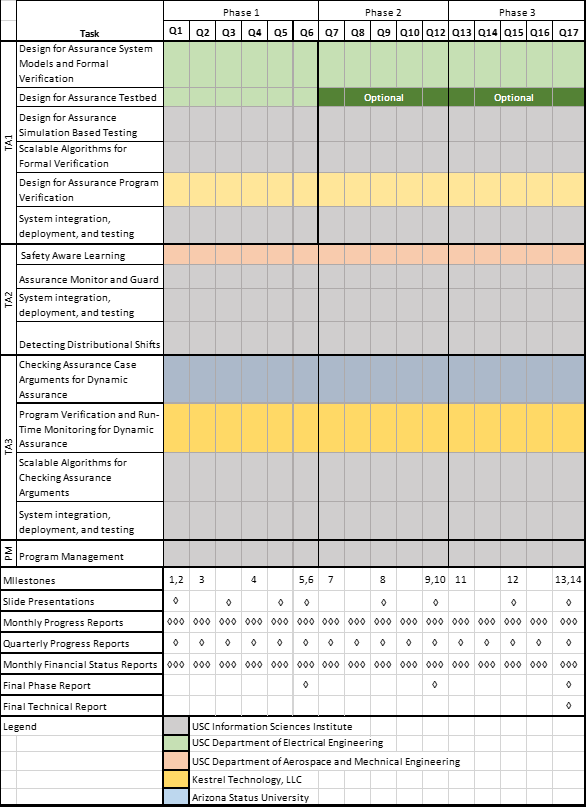
\includegraphics[width=.95\textwidth]{figs/Safeguard_Schedule_V6}
\end{center}
\vspace{-.2in}\caption{Project schedule along with a summary of milestones.  The legend maps task color to organization primary responsible for the task. } 
\label{fig:sandm}
\end{figure}
 

% \section{Level of Effort by Task \textcolor{red}{[Mike/Lisa - 1 pages]}}

% \textcolor{blue}{
% \begin{itemize}
% \item Will be a separate spreadsheet
% \item
% \end{itemize}
% }

\section*{Appendix A: Team Members and Other Information}
\addcontentsline{toc}{section}{Appendix A: Team Members and Other Information}

\baades{This section is mandatory and must include all of the following
components. If a particular subsection is not applicable, state “NONE”.}

\vspace{1ex}

\noindent
\textbf{Team Member Identification}:

\vspace{1ex}

\baades{Provide a list of all team members including the
prime, subcontractor(s), and consultant(s), as applicable. Identify specifically
whether any are a non-US organization or individual, FFRDC and/or Government
entity.}

\begin{centering}

%\small
\begin{tabular}{|p{1.8in}|p{1in}|p{1.1in}|p{0.7in}|p{0.8in}|p{0.7in}|}
\hline
 \textbf{Name} &  \textbf{Role} & \textbf{Organization} & \textbf{Non-US Org?}  & \textbf{Non-US Ind?} &  \textbf{FFRDC or Gov} \\
 \hline
Craig A. Knoblock & Prime & USC & N & N & N\\ \hline
Michael Orosz & Prime & USC & N &  N & N \\ \hline
Satish Thittamaranahalli & Prime & USC & N &  Y & N \\ \hline
Ryan Goodfellow & Prime & USC & N &  N & N \\ \hline
Anoop Kumar & Prime & USC & N & N & N \\ \hline
Satyandra Gupta & Prime & USC & N & N & N \\ \hline
Pierluigi Nuzzo & Prime & USC & N & Y & N \\ \hline
Petros Ioannou & Prime & USC & N & N & N \\ \hline
Chitta Baral & Subcontractor & ASU & N & N & N \\ \hline
Matt Barry & Subcontractor & Kestrel Technology & N & N & N \\ \hline
Douglas Smith & Subcontractor & Kestrel Technology & N & N & N \\ \hline
Henny Sipma & Subcontractor & Kestrel Technology & N & Y & N \\ \hline
\end{tabular} 
\end{centering}

\vspace{1ex}

\noindent
\textbf{Government or FFRDC Team Member Proof of Eligibility to Propose}: NONE

\baades {If
none of the team member organizations (prime or subcontractor) are a
Government entity or FFRDC, state “NONE”.}

\vspace{1ex}

\noindent
\textbf{Government or FFRDC Team Member Statement of Unique Capability}: NONE

\vspace{1ex}

\noindent
\textbf{Organizational Conflict of Interest Affirmations and Disclosure}: NONE

\vspace{1ex}

\noindent
\textbf{Intellectual Property (IP)}: 
\baades {
If no IP restrictions are intended, state “NONE”.
The Government will assume unlimited rights to all IP not explicitly identified as
having less than unlimited rights in the proposal.
For all technical data or computer software that will be furnished to the
Government with other than unlimited rights, provide (per Section VI.B.1) a list
describing all proprietary claims to results, prototypes, deliverables or systems
supporting and/or necessary for the use of the research, results, prototypes
and/or deliverables. Provide documentation proving ownership or possession of
appropriate licensing rights to all patented inventions (or inventions for which a
patent application has been filed) to be used for the proposed project.
}
\begin{centering}

%\small
\begin{tabular}{|p{2.1in}|p{1.2in}|p{1.4in}|p{2in}|}
\hline
\multicolumn{4}{|c|}{COMMERCIAL ITEMS }\\ \hline 
 \textbf{Technical Data, Computer Software To be Furnished With Restrictions} &  \textbf{Basis for Assertion} & \textbf{Asserted Rights Category} & \textbf{Name of Person Asserting Restrictions}  \\  \hline
KT Advance & Developed with mixed funding. & Restricted & David Kulich, Contracts Manager, Kestrel technology, LLC.\\ \hline
\end{tabular} 
\end{centering}

\vspace{1ex}

\noindent
\textbf{Human Subjects Research (HSR)}: NONE

\vspace{1ex}

\noindent
\textbf{Animal Use}: NONE

\vspace{1ex}

\noindent
\textbf{Representations Regarding Unpaid Delinquent Tax Liability or a Felony
Conviction under Any Federal Law}: 
%NONE

\begin{enumerate}
\item
The proposer is  not a corporation that has any unpaid Federal tax liability that has been assessed, for which all judicial and administrative remedies have been exhausted or have lapsed, and that is not being paid in a timely manner pursuant to an agreement with the authority responsible for collecting the tax liability,
\item
The proposer is not a corporation that was convicted of a felony criminal violation under a Federal law within the preceding 24 months.
\end{enumerate}

\vspace{1ex}

\noindent
\textbf{Cost Accounting Standards (CAS) Notices and Certification}:
\baades{
For any proposer who submits a proposal which, if accepted, will result in a CAS-compliant
contract, must include a Disclosure Statement as required by 48 CFR
9903.202. The disclosure forms may be found at
http://www.whitehouse.gov/omb/procurement\_casb
If this section is not applicable, state “NONE”. For further information regarding
this subject, please see www.darpa.mil/work-with-us/additional-baa.
}
NONE


%\section{Appendix B \textcolor{red}{[No Page Count]}}

\section{References}
\bibliographystyle{acm} 
\bibliography{TA3/ta3,TA2/ta2,TA1/ta1}
\end{document}
\clearpage
\newpage


\section{Management Plan}


The Principal Investigator for this effort is Dr. Craig Knoblock who is responsible for all aspects of the effort, will coordinate the parallel team efforts, and will ensure high levels of performance from individual team members.  The Co-P/I, Dr. Michael Orosz, will provide project management and will assist all performers in the execution of the project.    The project team is divided into three working groups (Figure~\ref{fig:org_chart}) corresponding to Technical Areas 1-3, however, members of each team contribute across all project activities.   Table~\ref{fig:Table_Mgmt} defines the major contributions of each project team member to the project tasks.

\begin{figure}[tbhp]
%\vspace{-25pt}
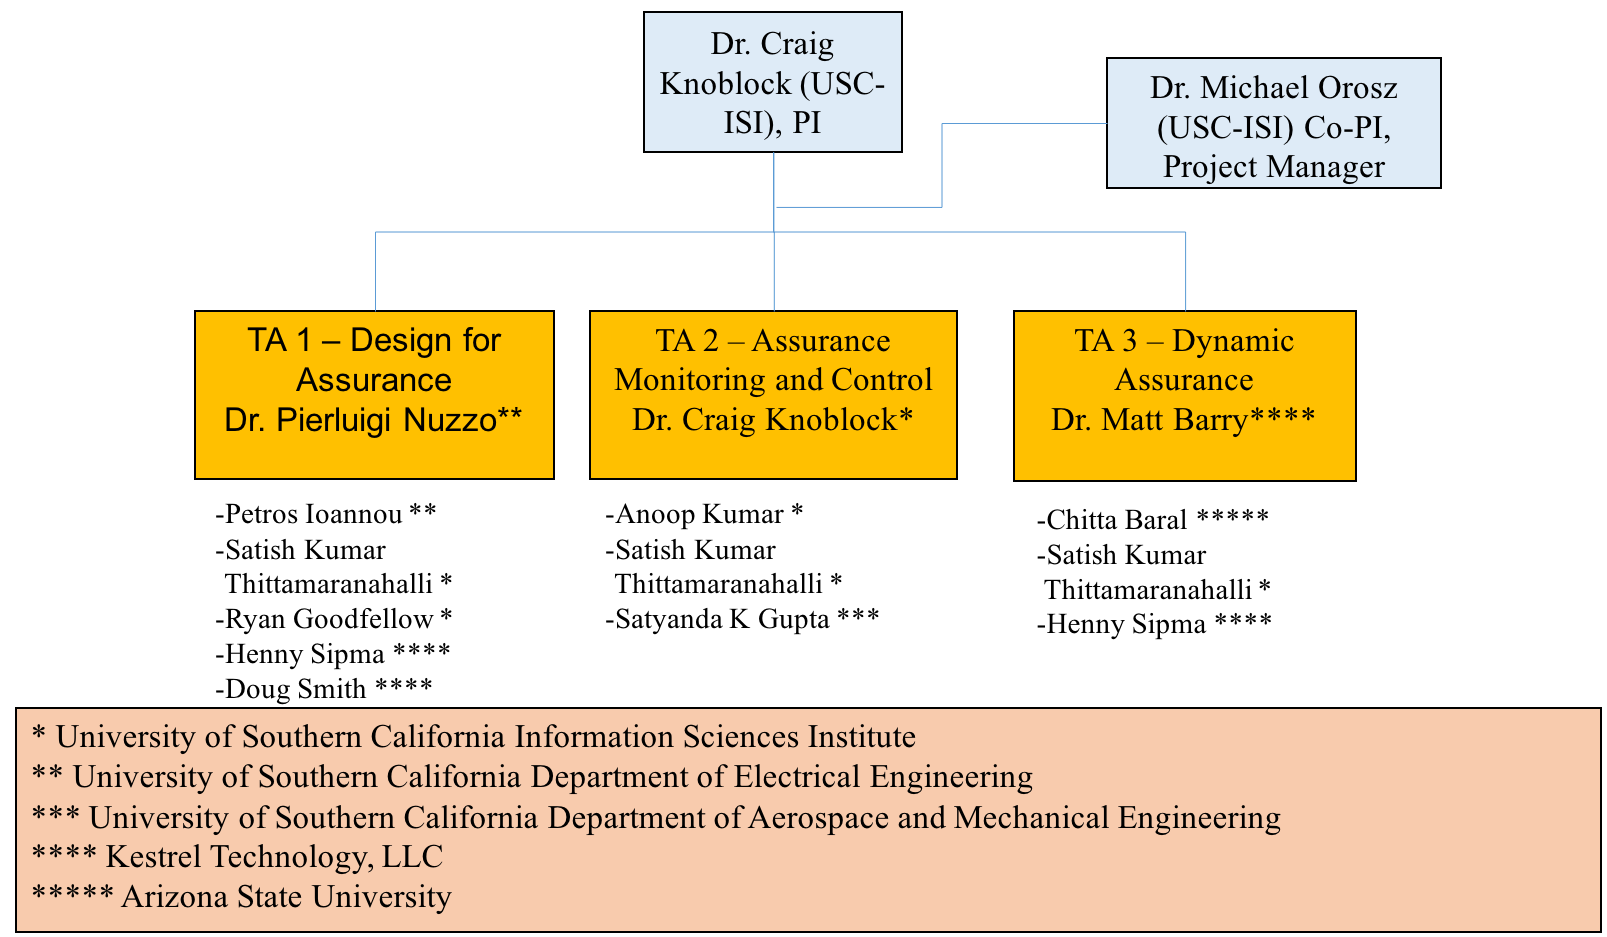
\includegraphics[width=6.0in]{./org-chart2.png}
\caption{\small Organization Chart}
\label{fig:org_chart}
\end{figure}

Coordination: To maximize collaboration and reduce risk to project failure from lack of communication and technical exchange, we plan to employ a wide variety of working styles and communication/coordination so that all can contribute.  At the core of our project will be regularly scheduled meetings bridging the diversely distributed team (Table~\ref{fig:Collaboration_Table}).  These meetings will address project status, identify challenges, implement risk mitigation strategies and participate in technology exchanges and system integration efforts (when appropriate)

\begin{table}[ht]
\caption{\small Project Meetings and Events}
  \centering
  {\footnotesize
\begin{tabular}{|m{3.15in}|m{3in}|} 
\hline
\textbf{Meeting} & \textbf{Frequency} 
\\\hline
Conference calls among investigators (discuss project status, address concerns and project risks) & Weekly
\\
\hline
Technical exchange and coordination meetings using Bluejeans or another videoconference technology & At least twice a month and more frequently as needed
  \\ 
\hline
Face-to-Face meetings (prior to P/I and demonstration meetings) & Every 3 to 6 months and more frequently (especially at the beginning of the project) as needed
 \\\cline{1-2}

\hline
\end{tabular}
}
\label{fig:Collaboration_Table}
\end{table}

\begin{table}[tbhp]
\caption{\small Key Project Team Member Responsibilities}
  \centering
  {\footnotesize
\begin{tabular}{| m{.75in} | m{3.9in}| m{1.5in}|} 
\hline
\textbf{Key Member} & \textbf{Responsibilities} & \textbf{Tasks} 
\\\hline
Dr.\ Craig Knoblock  & Principal Investigator responsible for project, leads TA 2 – Assurance Monitoring and Control.  Will lead the overall project and lead the TA2 team.  Served as the PI on many DARPA projects and has sucessfully led many large teams.    Effort on project:  25\% &
1.1.6, 1.2.2 1.2.3, 1.2.4, 1.3.4, 1.4.1, 
2.1.6, 2.2.2 2.2.3, 2.2.4, 2.3.4, 2.4.1, 
3.1.6, 3.2.2, 3.2.3, 3.2.4, 3.3.4, 3.4.1
\\
\hline
Dr.\ Michael Orosz & Co-Principal Investigator responsible managing the day-to-day operations of the project, assist technical teams as needed, coordinate with TA4 teams.    Has led many large complex multi-disciplined/multi-organizational projects in academic and industry environments.  Effort on project: 50\%
& 1.1.6, 2.1.6, 3.1.6, 1.4.1, 2.4.1, 3.4.1
  \\ 
\hline
Dr.\ Pierluigi Nuzzo 
& 
Co-Principal Investigator.  Leads the TA 1 - Design for Assurance team and conducts research on the formal methods for the design of the TA1 system.  Research experience on methodologies and tools for the design of cyber-physical systems; contracts, interfaces, and compositional methods for embedded system design; the application of automated formal methods and optimization theory to problems in embedded and cyber-physical systems.  Effort on project: 2 months/year (16.6\%)
& 
1.1.1, 2.1.1, 3.1.1 \\
\hline
Dr.\ Matthew Barry
& 
Key personnel.  Leads the TA 3 – Dynamic Assurance.   He will conduct the research on the dynamic assurance case language editors and parsers, the run-time system, and system integrations. Effort on project:  66\%
& 
1.3.2, 2.3.2, 3.3.2\\
\hline
Dr.\ Chitta Baral
& 
Key personnel responsible for learning assurance rules, supporting assurance rules with uncertainty and improving solver speed.  Expertise on ASP solvers, which will be used to reason about the assurance cases. Effort on project: 20\%
& 
1.3.1, 2.3.1, 3.3.1 \\
\hline
Dr.\ Doug Smith 
& 
Key personnel will support formal methods aspects of TA1, and lead the effort on abstract refinement. Expertise in field of automated correct-by-construction program generation.    Effort on project: 40\%
& 
1.1.5, 2.1.5, 3.1.5 \\
\hline
Dr.\ Henny Sipma
& 
Key personnel who will support the program verification tasks under TA1.  Will lead the effort on program verification.   Effort on project:  45\%
& 
1.1.5, 2.1.5, 3.1.5, 1.3.2, 2.3.2, 3.3.2 \\
\hline
Dr.\ Petros Ioannou
& 
Key personnel responsible providing and extending the assurance test bed, which will be available at the start of the project for autonomous vehicles.   Effort on project: 1 month/year (8.3\%)
& 
1.1.2, 2.1.2 (optional), 3.1.2 (optional)
\\
\hline
Dr.\ Satyandra Kumar Gupta
& 
Key Personnel providing autonomous command and control expertise to the TA-2 team.   Will lead the research on safety aware learning on TA2.   Past research on physics-aware decision making to facilitate automation.  Effort on project: 1 month/year (8.3\%)
& 
1.2.1, 2.2.1, 3.2.1 \\
\hline
Dr.\ Anoop Kumar 
& 
Key personnel providing support to the TA 2 project team.  Will lead the research on monitoring \& control and detecting distribution shifts.  Effort on project: 50\%
& 
1.2.1, 1.2.2, 1.2.3, 1.2.4, 2.2.1, 2.2.2, 2.2.3, 2.2.4, 3.2.1, 3.2.2, 3.2.3, 3.2.4\\
\hline
Dr.\ Satish Thittamaranahalli
& 
Key personnel developing scalable algorithms for TA1, TA2, and TA3 project teams.  Has extensive experience on scalable algorithm design, machine learning, and constraint reasoning.  Effort on project: 50\%
& 
1.2.1, 1.2.2, 1.2.3, 1.2.4, 2.2.1, 2.2.2, 2.2.3, 2.2.4, 3.2.1, 3.2.2, 3.2.3, 3.2.4, 1.1.4, 2.1.4, 3.1.4 \\
\hline
Dr.\ Ryan Goodfellow
& 
Key personnel providing support to the TA-1 project. Will lead the research on simulation-based testing.  Has extensive experience on simulation-based testing.  Effort on project:  30\%
& 
1.1.3, 2.1.3, 3.1.3 \\

\cline{1-2}

\hline
\end{tabular}
}
\label{fig:Table_Mgmt}
\end{table}



\newpage
\section{Personnel, Qualifications and Commitment}

{\bf Dr.\ Craig Knoblock}, the PI on this effort, is a Research Professor of both Computer Science and Spatial Sciences at the University of Southern California (USC) and Director of the Intelligent Systems Division at the USC Information Sciences Institute.   He received his Ph.D. from Carnegie Mellon University in computer science. 
%His research focuses on techniques for describing, acquiring, and exploiting the semantics of data.  
In previous projects he has worked on developing  scalable approaches to execution monitoring, accurate detection of sensor failures, and   automatic modeling and reconstruction of sensors.  He has published more than 300 journal articles, book chapters, and conference papers on these topics.  Dr. Knoblock is a Fellow of the Association for the Advancement of Artificial Intelligence (AAAI), a Distinguished Scientist of the Association of Computing Machinery (ACM), a Senior Member of IEEE, past President and Trustee of the International Joint Conference on Artificial Intelligence.
%and winner of the 2014 Robert S. Engelmore Award.  

{\bf Dr.\ Michael Orosz}, a Co-PI on this effort, is a Research Associate Professor of Civil and Environmental Engineering at the University of Southern California (USC) and Research Director of the Decision Systems Group at the USC Information Sciences Institute.  Dr. Orosz has over 30 years’ experience in commercial and government software development, basic and applied research, project management, academic research and has developed and deployed several commercially successful products.  His research interests are in machine learning and decision analytics as applied to intelligence analysis and autonomous command and control such as smart building controls.    Dr. Orosz has extensive experience in managing large complex multi-disciplined/multi-teamed research projects. %funded by DARPA, DHS, DoD, DoE, Industry, NASA, NRO, NSA and ONR.   
He received his Ph.D. in computer science from the University of California, Los Angeles.

{\bf Dr.\ Pierluigi Nuzzo}, a Co-PI on this project, is an Assistant Professor in the Department of Electrical Engineering at the University of Southern California. He received the Ph.D. in Electrical Engineering and Computer Sciences from the University of California at Berkeley. 
%in 2015, and the Laurea degree (MS) in electrical engineering (summa cum laude) from the University of Pisa, Italy, and the Sant'Anna School of Advanced Studies, Pisa, Italy.
%
%He has four years of research experience in analog and mixed signal circuit design as a researcher at IMEC, Leuven, Belgium, and over 10 years experience in design methodologies and tools for mixed-signal integrated circuits and cyber-physical systems, as a researcher at the University of Pisa, IMEC, UC Berkeley, and USC. 
His research interests
include: methodologies and tools for cyber-physical system and mixed-signal
system design; contracts, interfaces and compositional methods for embedded
system design; the application of formal methods and optimization theory to problems in embedded and cyber-physical systems and electronic design automation. 
%
Prof. Nuzzo received %First Place in the operational category and Best Overall
%Submission in the 2006 DAC/ISSCC Design Competition, 
a Marie Curie Fellowship
from the European Union in 2006, 
the University of California at Berkeley EECS
departmental fellowship in 2008, 
%the University of California at Berkeley Outstanding Graduate Student Instructor Award in 2013, 
the IBM Ph.D.
Fellowship in 2012 and 2014, 
%the Best Paper Award from the International Conference on Cyber-Physical Systems (ICCPS) in 2016, 
and the David J.~Sakrison Memorial Prize in 2016 for his doctoral research. 
%He is an author of 1 patent and over 60 publications.

{\bf Dr.\ Satyandra K. Gupta} is Smith International Professor in the Department of Aerospace and Mechanical Engineering at the University of Southern California. %Prior to joining the University of Southern California, he was a Professor in the Department of Mechanical Engineering and the Institute for Systems Research at the University of Maryland. He was the founding director of the Maryland Robotics Center and the Advanced Manufacturing Laboratory at the University of Maryland. 
He served as a program director for the National Robotics Initiative at the National Science Foundation from September 2012 to September 2014.  Dr. Gupta's interest is in the area of physics-aware decision making to facilitate automation. He has published more than 300 technical articles. He is a fellow of the American Society of Mechanical Engineers (ASME) and editor of ASME Journal of Computing and Information Science in Engineering. Dr. Gupta has received the Young Investigator Award from the Office of Naval Research in 2000, CAREER Award from the National Science Foundation in 2001, Presidential Early Career Award for Scientists and Engineers (PECASE) in 2001, Invention of the Year Award at the University of Maryland in 2007, Kos Ishii-Toshiba Award from ASME in 2011, and Excellence in Research Award from ASME in 2013.%, and Distinguished Alumnus Award from Indian Institute of Technology, Roorkee in 2014. %He has also received seven best paper awards at conferences.

{\bf Ryan Goodfellow} is a computer scientist at ISI working in combined cyber physical simulation and emulation platform development. His formal background is in simulation algorithms and modeling techniques using differential-algebraic equations (DAE). He has applied this knowledge in the CPS space by integrating DAE modeling languages and simulation engines with network testbeds to create comprehensive scientific experimentation platforms for cyber-physical systems. These experimentation platforms have been used in the power grid research space. %Ryan is a lead developer on the Deter network testbed, with a strong background in networked and distributed systems engineering. %He is also a combat veteran, serving as a non-commissioned officer and SIGINT team lead for a multi-functional intelligence team in Afghanistan.

{\bf Dr.\ Petros Ioannou} is a Professor in the Department of Electrical Engineering, Director of the Center for Advanced Transportation Technologies and Associate Director for Research for the DOT supported University Transportation Center at USC. He received his MS and PhD from the University of Illinois at Urbana Champaign in Mechanical and Electrical Engineering, respectively. His research interests are in robust adaptive control, vehicle dynamics and control, human factors and safety, automated vehicles, nonlinear systems and Intelligent transportation Systems.  He received the 2016 IEEE Transportation Technologies field award and the 2016 IEEE Control system society Transition to Practice Award. He is a Fellow of IEEE, IFAC and IET and author/coauthor of 8 books and over 400 papers.

{\bf Dr.\ Matthew Barry} will serve as lead for the TA3 tasks. %He will implement the dynamic assurance case language editors and parsers, the run-time system, and system integrations.  He will implement the assurance case arguments and the API for updating argument structure and content.  
Dr. Barry currently is CEO at Kestrel Technology LLC, and previously spent 20 years in NASA space mission operations at the Jet Propulsion Lab and Johnson Space Center.  At NASA Headquarters he led the introduction of dependability case requirements and plans for flight computing systems in upcoming manned space exploration missions, as well as the development of Agency-level software-related safety-critical control system requirements.  He recently served as a Principal Investigator on DHS/Cyber S\&T STAMP (Static Tool Analysis Modernization Program), DARPA CSFV (Crowd Sourced Formal Verification), three NASA Aeronautics R\&D projects, and the AFRL-sponsored Static Analysis of Numerical Algorithms project.  Dr. Barry earned BSME, MS, and PhD degrees in mechanical engineering, and an MBA degree, from Rice University.  

{\bf Dr.\ Henny Sipma} will support the program verification tasks under TA1.  %She is the key person behind the company's {\em KT Advance\/} and {\em KT Transferal\/} static analysis products, and the designer and programmer of the company's core {\em CodeHawk\/} abstract interpretation engine. 
Dr. Sipma currently is the CTO at Kestrel Technology LLC.  She has spent the past 10 years with Kestrel Technology as a static analysis expert; previously developed and taught static analysis techniques as senior research associate at Stanford University for eight years; and developed industrial process controls as an senior systems analyst at Shell.  She has been Principal Investigator or company lead on several recent R\&D projects for Federal agencies, including two projects under the IARPA STONESOUP (Securely Taking On New Executable Software of Uncertain Provenance) program; the DHS Cyber S\&T Gold Standard project; and the DARPA-sponsored STAC (Space-Time Analysis for Cybersecurity) and MUSE (Mining and Understanding Software Enclaves) programs.  Dr. Sipma earned 
%a BS degree in chemistry and an MS degree in chemical engineering at the University of Groningen in The Netherlands, and 
MS and PhD degrees in computer science from Stanford University.  

{\bf Dr.\ Douglas R.\ Smith} will support formal methods aspects of TA1, including the enforcement of safety properties and the generation of monitors.  He is President of Kestrel Technology LLC and Principal Scientist at Kestrel Institute.  He is a Fellow of the American Association of Artificial Intelligence (AAAI) and an ASE Fellow (Automated Software Engineering).  From 1986 to 2000, he taught an advanced graduate course on correct-by-construction software development at Stanford.  
%Dr. Smith has led the development of a series of software synthesis systems, including KIDS (Kestrel Interactive Development System), Specware, Designware, and Planware. 
%Applications domains have included a variety of complex high-performance planners and schedulers for the US Air Force.  He leads current projects on the generation of air mission plans and cyberoperations.  
Other recent projects focused on automated policy enforcement \cite{SmithD0703,SmithD08}, synthesis of secure network protocol codes, and the synthesis of high-performance constraint-solvers\cite{SmithD08c,SmithD13}.  Dr. Smith has over 30 years experience in the field of automated correct-by-construction program generation and has published over 100 papers. He has one patent.  He received the Ph.D. in Computer Science from Duke University% in 1979.  

{\bf Dr. Chitta Baral} is a Professor in the Department of Computer Science and Engineering at Arizona State University. He will support the TA3 efforts on Learning assurance rules, supporting assurance rules with uncertainty and improving solver speed. Dr. Baral has expertise in various aspects of autonomy and Artificial Intelligence. 
He wrote the first book on answer set programming (published by Cambridge University Press) the formal language behind our assurance rules. Some of his other works relevant to this proposal are: goal specification for autonomous systems, automatic construction of control rules for autonomous systems that satisfy given goals, combining machine learning with reasoning in various contexts, including image understanding. %He is the President of KR Inc. He is an associate editor of AIJ and has been an associate editor of JAIR.

{\bf Dr.\ Satish Kumar Thittamaranahalli (T. K. Satish Kumar)} leads the Collaboratory for Algorithmic Techniques and Artificial Intelligence (CATAI) at USC's Information Sciences Institute. He has published over 60 papers on numerous topics in Artificial Intelligence spanning such diverse areas as Constraint Reasoning, Planning and Scheduling, Probabilistic Reasoning, Robotics, Combinatorial Optimization, Approximation and Randomization, Heuristic Search, Model-Based Reasoning, Knowledge Representation and Spatio-Temporal Reasoning. %He %has served on the Program Committees of many international conferences in Artificial Intelligence
He and is a winner of the 2016 Best Robotics Paper Award and the 2005 Best Student Paper Award from the International Conference on Automated Planning and Scheduling. 
Dr. Kumar received his PhD in Computer Science from Stanford University. %In the past, he has also been a Visiting Student at the NASA Ames Research Center, a Postdoctoral Research Scholar at the University of California, Berkeley, a Research Scientist at the Institute for Human and Machine Cognition, a Visiting Assistant Professor at the University of West Florida, and a Senior Research and Development Scientist at Mission Critical Technologies.

\textbf{Dr.\ Anoop Kumar} is a senior computer scientist at USC ISI and has broad expertise in machine learning, statistical modeling, and software engineering.  Dr.\ Kumar is the technical lead on the DARPA RSPACE program and has played a vital role in developing a system that fuses air operations data from multiple sources, maintains world state, and issues warnings. Previously, he led the research and development of the BBN’s election forecasting system for the IARPA OSI program. %Dr.\ Kumar played a significant role in the DARPA DEFT program by developing a model to support integration of output from multiple NLP algorithms. He has contributed at the development to management levels on government research contracts and commercial projects. 
Dr.\ Kumar helped design and develop BBN's commercially available, hosted speech and medical transcription services offering. 

\begin{table}[!tbh]
\begin{footnotesize}
\vspace{-0.1in}

\begin{tabular}{lll}
\begin{tabular}[t]{|l|@{}c@{}|@{}c@{}|@{}c@{}|@{}c@{}|} \hline
Project & Status & \multicolumn{3}{ c| }{Hours} \\ \cline{3-5}
& & P1 & P2 & P3 \\ \hline



\multicolumn{5}{ |c| }{ \textbf{Craig Knoblock} } \\ \cline{1-5}
Safeguard & Pro & 770 & 641 & 641 \\ \cline{1-5}
ELICIT & Cur & 308 & 256 & 120 \\ \cline{1-5}
WTNIC & Cur & 11 & 0 & 0 \\ \cline{1-5}
EFFECT & Cur & 641 & 107 & 0 \\ \cline{1-5}
LinkedMaps & Cur & 203 & 25 & 0 \\ \cline{1-5}
PRINCESS & Cur & 608 & 96 & 0 \\ \cline{1-5}
SCHARP & Cur & 481 & 54 & 0 \\ \cline{1-5}
MINT & Pen & 650 & 534 & 285 \\ \cline{1-5}

\multicolumn{5}{ |c| }{ \textbf{Michael Orosz} } \\ \cline{1-5}
Safeguard & Pro & 1560 & 1300 & 1300  \\ \cline{1-5}
SMC/SY & Cur & 1803 & 0 & 0  \\ \cline{1-5}

\multicolumn{5}{ |c| }{ \textbf{Matthew Barry} } \\ \cline{1-5}
Safeguard & Pro & 2078 & 1690 & 1554 \\ \cline{1-5}
Starlite & Cur & 1840 & 1692 & 0 \\ \cline{1-5}



\multicolumn{5}{ |c| }{ \textbf{Anoop Kumar} } \\ \cline{1-5}
Safeguard & Pro & 1560 & 1300 & 1300 \\ \cline{1-5}

\end{tabular}
&
\begin{tabular}[t]{|l|@{}c@{}|@{}c@{}|@{}c@{}|@{}c@{}|} \hline
Project & Status & \multicolumn{3}{ c| }{Hours} \\ \cline{3-5}
& & P1 & P2 & P3 \\ \hline

\multicolumn{5}{ |c| }{ \textbf{Pierluigi Nuzzo} } \\ \cline{1-5}
Safeguard & Pro & 520 & 433 & 433  \\ \cline{1-5}
Mirage & Cur & 433 & 0 & 0  \\ \cline{1-5}

\multicolumn{5}{ |c| }{ \textbf{Satyandra Gupta} } \\ \cline{1-5}
Safeguard & Pro & 260 & 217 & 217 \\ \cline{1-5}
Human   & Cur & 22 & 0 & 0 \\ \cline{1-5}
Vehicles & Cur & 36 & 0 & 0 \\ \cline{1-5}
Robot & Cur & 116 & 0 & 0 \\ \cline{1-5}
Assembly & Cur & 33 & 0 & 0 \\ \cline{1-5}
Solar & Cur & 4 & 0 & 0 \\ \cline{1-5}

\multicolumn{5}{ |c| }{ \textbf{Petros Ioannou} } \\ \cline{1-5}
Safeguard & Pro & 260 & 217 & 217 \\ \cline{1-5}
CPS & Cur & 130 & 0 & 0 \\ \cline{1-5}

\multicolumn{5}{ |c| }{ \textbf{Ryan Goodfellow} } \\ \cline{1-5}
Safeguard & Pro & 936 & 780 & 780 \\ \cline{1-5}
STEAM & Cur & 416 & 0 & 0 \\ \cline{1-5}


\end{tabular}
&
\begin{tabular}[t]{|l|@{}c@{}|@{}c@{}|@{}c@{}|@{}c@{}|} \hline
Project & Status & \multicolumn{3}{ c| }{Hours} \\ \cline{3-5}
& & P1 & P2 & P3 \\ \hline

\multicolumn{5}{ |c| }{ \textbf{Chitta Baral} } \\ \cline{1-5}
Safeguard & Pro & 659 & 485 & 485 \\ \cline{1-5}
PostdocBP & Cur & 176 & 0 & 0 \\ \cline{1-5}
Languages & Pen & 528 & 264 & 264 \\ \cline{1-5}
CAREER & Pen & 88 & 44 & 44 \\ \cline{1-5}
CHS & Pen & 510 & 255 & 0 \\ \cline{1-5}

\multicolumn{5}{ |c| }{ \textbf{Doug Smith} } \\ \cline{1-5}
Safeguard & Pro & 1222 & 984 & 840 \\ \cline{1-5}
RSPACE & Cur & 342 & 0 & 0 \\ 
\cline{1-5}
PLANX & Cur & 154 & 0 & 0 \\ 
\cline{1-5}
HACCS & Pen & 923 & 769 & 769 \\ 
\cline{1-5}

\multicolumn{5}{ |c| }{ \textbf{Henny Sipma} } \\ \cline{1-5}
Safeguard & Pro & 1372 & 962 & 840 \\ \cline{1-5}
STAC & Cur & 797 & 0 & 0 \\ \cline{1-5}

\multicolumn{5}{ |c| }{ \textbf{Satish Thittamaranahalli} } \\ \cline{1-5}
Safeguard & Pro & 1560 & 1300 & 1300 \\ \cline{1-5}
MapF & Cur & 103 & 103 & 0 \\ \cline{1-5}

\end{tabular}
\end{tabular}

\end{footnotesize}
\caption{Individual commitments of key personnel}
\label{tab:Commitments}
\vspace{-0.2in}
\end{table}

\clearpage
\newpage
\section{Capabilities}


%\subsection{University of Southern California}
USC has strengths in number of areas that are closely related to the proposed work:
\begin{itemize}[itemsep=0pt,leftmargin=*]
\item Dr.\ Nuzzo 
%has over 10-year research experience in embedded system design, from mixed-signal chip design (analog-to-digital converters, frequency synthesizers, software-defined radio), to methodologies and tools for mixed-signal integrated circuits and Cyber-Physical Systems (CPSs), and the application of formal methods and optimization theory to problems in embedded and cyber-physical systems and electronic design automation.  
%His doctoral work 
has done extensive research on contracts and compositional methods for heterogeneous system design and design space exploration, with application to aircraft electric power systems and environmental control systems. His work has helped transition rigorous system design foundations, innovative design methodologies, and new systems engineering paradigms to industry (IBM, United Technologies). 
\item Dr.\ Satyandra K. Gupta has worked on autonomous surface vehicles, autonomous ground vehicles for operation on rugged terrains, and autonomous flapping wing aerial vehicles.   His group has developed a hierarchal decision making approach for realizing autonomous systems. 
%This approach combines task planning and assignment, deliberative trajectory planning, reactive collision avoidance behaviors, and trajectory tracking control layers. 
His group has also developed new methods for learning reactive behaviors in adversarial environments and COLREGS compliant trajectory planning. \item Dr.\ Knoblock has developed methods that learn the relationships between sensors to both identify failures and changes in sensor and reconstruct those sensors, providing estimates of the accuracy of the reconstructed sensors.  
\item Ryan Goodfellow has extensive experience in simulation based testing through high-fidelity CPS testbed environment development and operation, using the Deter network testbed as the core which has supported several large scale government projects from a variety of agencies and thousands of users. %we have developed sophisticated CPS experiments under programs such as NFS RIPS, NIST SmartCities and the DHS Cybersecurity showcase.
\item Dr.\ Ioannou %helped  design and implement adaptive cruise control systems in collaboration with Ford Motor Company, which was commercialized four years before any other company. He 
worked on several DOT funded projects on automated vehicles and intelligent highway systems where he demonstrated his vehicle control designs for safety and performance on actual automated vehicles in test trucks and I-15 highway.
\item Drs.\ Knoblock, Kumar, and Thittamaranahalli have developed highly scalable approaches for monitoring message traffic to identify potential problems and issue warnings and alerts. 
\item Dr. Thittamaranahalli has developed state-of-the-art methods for efficiently solving large-scale search and optimization problems. %These techniques will be applicable in TA2 for safety-aware learning and planning, in TA2 for assurance monitoring and control, and in TA3 for dynamic assessment of assurance cases.

\end{itemize}
%\subsection{Kestrel Technology LLC}

Kestrel Technology's strength is in program analysis, specifically static analysis of both source and binary targets.  The company performs applied R\&D and product development for a variety of static analysis applications  pivoting primarily on the abstract interpretation technique.  The company recently initiated development of program analysis applications using logical equivalence techniques. As a provider of verification evidence in the form of mathematical proofs, the company also has expertise in the design and development of assurance case arguments for high-integrity systems using such evidence. %The company is engaged in a partnership with Wind River Systems to develop program analysis tools for its embedded system developers.  Many of Wind River's customers must develop their products under safety and certification standards, including those using safety cases.  

   

%\subsection{Arizona State University}
Chitta Baral at Arizona State University has developed various software to learn assurance rules and various ASP solvers, which he has made available as open-source.

Most of the software carried forward for implementation or derivation is open source.  The single exception is Kestrel Technology's {\it KT Advance\/} static analysis tool (TA1), in particular the abstract interpretation engine therein, which is company proprietary and is US EAR export-controlled.   
%Owing to mixed funding for the development of that technology 
We will continue to provide the Federal government a restricted use license for that particular item.

There are no specialized facilities, data, or GFE required for this effort. 


\section{Statement of Work}
We propose work for TA 1 – TA 3 for all three phases. All tasks span the four years of the program. For each task we provide an objective, the high-level approach (focusing on the responsibilities of each contributing organization), and the specific approach and milestones planned for each task for each phase. On all tasks, we will deliver design documents, software implementations, demonstrations, and publications. With the exception of several tasks accomplished by Kesler Technology, LLC, all tasks that accomplished at a university (USC/ISI, USC, and ASU) are believed to be fundamental research.   
%\usepackage[table]{xcolor}

{\scriptsize

\begin{longtable} {|p{\textwidth} | }

\hline

\textcolor{blue} {\footnotesize {\textbf{Tasks 1.1.1, 2.1.1, 3.1.1 -Design for Assurance System Models and Formal Verification (USC)}}} \\ \hline
Objective:  Develop contract-based formalisms and mapping tools to represent and reason about LE-CPSs at multiple levels of abstraction and generate assurance cases.  Undertake scalable formal verification and synthesis via Satisfiability Modulo Convex Programming. \\ \hline
Approach:  Develop modeling formalisms to represent components and contracts for LE-CPSs, including physical plant (e.g., autonomous vehicle, sensors, actuators, environment, controllers, and learning components. Formalisms will encompass different control and learning architectures (e.g., neural networks, statistical methods, graphical models, ensemble methods, decision trees) and support mapping between abstractions.   Develop a formal domain-specific language to capture and formalize requirements on LE components, systems, and their dynamics as contracts.   Develop a unifying framework and efficient algorithms to reason about the combination of discrete and continuous dynamics and constraints in the presence of uncertainties in LE cyber-physical systems \\ \hline
Phase 1 (1.1.1):  Milestone 1: Develop initial design followed by development and testing of individual components.  Milestone 2:  Library of components and contracts for the autonomous vehicle application driver.  Milestone 4: Library of components and contracts for the platforms provided by TA4 performers. Extension of the methodology and to support up to 20 continuous dimensions and 2 learning components for the 2 application drivers from TA4.  Milestone 6: -Prototype toolkit (software package) for capturing requirements, for translating them into contracts, for analyzing and validating them using contract operations and relations.  Prototype toolkit for capturing probabilistic requirements and behaviors of LE components, systems, and their dynamics, for translating them into stochastic assume-guarantee contracts, for analyzing and validating them using contract operations and relations, and for synthesizing design and verification artifacts from contracts.  Extension of the SMC framework and toolkit to support reactive and robust task and trajectory planning in the presence of uncertainties. \\ \hline
Phase 2 (2.1.1) Milestone 7: Refinement of design.  Milestone 9: extension of methodology, design, toolkits and libraries to support 40 continuous dimensions, 4 LECs, 30\% monitoring overhead. Extension of the SMC framework and toolkit from Phase 1 to support verification and synthesis on system with 40 dimensions and 4 LECs.  Milestone 10: Demonstration of the SMC framework and toolkit.  Contribution to Phase II report and dissemination of the results in conferences and journals. \\ \hline
Phase 3 (3.1.1) Milestone 11: Update design based on Phase II demo.  Milestones 12-13:  extend methodology, design, toolkits and libraries to support 100 dimensions, 6 LECs and 10\% monitoring overhead.   Milestone 14: Undertake Phase III demonstration on both platforms and submit final project report. \\ \hline
\textcolor{blue} {\footnotesize {\textbf{Tasks 1.1.2, 2.1.2, 3.1.2: Design for Assurance Testbed (USC)} }}\\ \hline
Objective:  Develop a simulation test bed for data generation and LE algorithm testing, redesign and/or refinement.   Simulator used as the test bed until the TA4 platforms are available.   Test bed will be used for internal research/prototype after TA4 platform availability. \\ \hline
Approach:  Leverage previous work on microscopic traffic simulations in urban and rural environments using the commercial software VISSIM and Vortex Studio and built in extensions for automated driving.   Develop testbed for autonomous vehicles in road/off-road environments to allow LEs to collect data, learn and make control decisions on line and in real time by simulating scenarios. The testbed together with analytical tools used to refine and redesign LEs and control algorithms by taking into account effects revealed by the simulation and not accounted for in the design stage.    In the event the TA4 platforms are not available, the test bed will be extended further by integrating all the LE components, controllers and sensors for demonstration purposes and evaluation of the proposed methodology. \\ \hline
Phase 1 (1.1.2):  Milestones 1-2:  Extension of existing simulator test beds.  Milestones 3-5:  Testing of individual components under normal and unpredicatble situations and demonstrating the results in VISSIM under several different driving scenarios. \\ \hline
Phase 2 (2.1.2) – Optional:  Milestones 7-8:  Extension of existing simulator test beds to support the TA1-TA3 teams.  Milestones 9-10:  Support demonstration of technology capable of supporting 40 dimensions, 4 LECs and 30\% monitoring overhead. \\ \hline
Phase 3 (3.1.2) – Optional:  Milestones 11-12:  Extension of existing simulator test beds to support the TA1-TA3 teams.  Milestones 13-14:  Support demonstration of technology capable of supporting 100 dimensions, 6 LECs and 10\% monitoring overhead. \\ \hline
\textcolor{blue} {\footnotesize {\textbf{Tasks 1.1.3, 2.1.3, 3.1.3: Design for Assurance Simulation Based Testing (USC/ISI)}}} \\ \hline
Objective:  Develop external Discrete Control Mechanisms for OpenModelica.  Develop/package virtual-machine based static time dilation systems. Undertake network testbed integration and develop physical system behavioral analysis tooling. \\ \hline
Approach:  Leverage previous external discrete control mechanisms for DAEs, implement similar facilities for OpenModelica to allow LEs to observe and control a physical system over a network. Contributions pushed back upstream to OpenModelica project.  Implement DieCast for modern libvirt.  Develop tooling to deploy integrated CPS models on the Deter network testbed. Apply modern DAE control theory in the form Modelica analysis packages usable by non DAE experts. \\ \hline
Phase 1 (1.1.3):  Milestones 1-2:  Initial CPS simulation concept and components.  Milestones 3-5:  Testing of individual components under normal and unpredictable situations and demonstrating the results capable of meeting 20 dimensions, 2 LECs and 50\% or under monitoring overhead conditions.   Milestone 6: Demonstrate technology in Phase I demonstration, contribute to Phase I final report and disseminate software and publications. \\ \hline
Phase 2 (2.1.3):  Milestones 7-8:  Apply lessons learned from Phase I and extend existing simulations to support 30 dimensions, 3 LECs and 40\% monitoring overhead.  Milestones 9-10:  Support demonstration of technology capable of supporting 40 dimensions, 4 LECs and 30\% monitoring overhead.  Contribute to Phase II final report and disseminate software and publications. \\ \hline
Phase 3 (3.1.3):  Milestones 11-12:  Apply lessons learned from Phase II and extend existing simulations to support 70 dimensions, 5 LECs and 20\% monitoring overhead.  Milestones 13-14:  Support demonstration of technology capable of supporting 100 dimensions, 6 LECs and 10\% monitoring overhead.  Contribute to Phase III final report and disseminate software and publications. \\ \hline
\textcolor{blue} {\footnotesize {\textbf{Tasks 1.1.4, 2.1.4, 3.1.4: Scalable Algorithms for Formal Verification (USC/ISI)}}} \\ \hline
Objective: Develop innovative algorithms for scalable formal verification. \\ \hline
Approach: Use state-of-the-art techniques for solving combinatorial problems with discrete/continuous variables and hybrid constraints. \\ \hline
Phase 1 (Task 1.1.4): Milestones 1-2: Develop initial design plan and initial concepts. Milestones 3-5: Integrate framework that is capable of supporting 20 dimensions, 2 LECs and 0.1x trials to assurance. Milestone 6: Participate in Phase I demonstration, contribute to Phase I final report and disseminate software and publications. \\ \hline
Phase 2 (Task 2.1.4): Milestones 7-8: Apply lessons learned from Phase I and extend existing design to support 30 dimensions, 3 LECs and 0.05x trials to assurance. Milestones 9-10: Demonstrate technology capable of supporting 40 dimensions, 4 LECs and 0.01x trials to assurance. Participate in Phase II demonstration, contribute to Phase II final report and disseminate software and publications. \\ \hline
Phase 3 (Task 3.1.4): Milestones 11-12: Apply lessons learned from Phase II and extend design/approach to support 70 dimensions, 5 LECs and 0.005x trials to assurance. Milestones 13-14: Demonstrate technology capable of supporting 100 dimensions, 6 LECs and 0.001x trials to assurance. Complete integration of technology into TA4 platform. Contribute to Phase III final report and disseminate software and publications. \\ \hline
\textcolor{blue} {\footnotesize {\textbf{Tasks 1.1.5, 2.1.5, 3.1.5: Design for Assurance Program Verification (Kestrel Technology, LLC)}}} \\ \hline
Objective: Develop and integrate program analysis and monitor synthesis functionality with TA1 functions and services and integrate combined TA1 functions with TA4 platform. \\ \hline
Approach: Integrate existing analysis tools into development environment.  Design and implement abstract domains and properties for one or more modeling layers.  Design and implement analyzer front-end for modeling layers.  Implement test framework for verification tools.  Implement content providers and/or consumers for DAC via DAC API.  Leverage existing algorithms and tools to generate monitors for assumptions and unproven safety constraints. Integrate program analysis and monitor synthesis functionality with TA1 functions and services, integrate combined TA1 functions with TA4 platform.   Prepare software and data installation kits and operating instructions;install software and confirm configuration. \\ \hline
Phase 1 (1.1.5) : Milestones 1-2:  Initial framework design and unit tools, TA1-TA3 interfaces defined. Milestones 3-5:  Testing of individual components/tools capable of meeting 20 dimensions, 2 LECs and 50\% or under monitoring overhead conditions.   Milestone 6: Demonstrate technology in Phase I demonstration, contribute to Phase I final report and disseminate software and publications. \\ \hline
Phase 2 (2.1.5): Milestones 7-8:  Apply lessons learned from Phase I and extend existing design to support 30 dimensions, 3 LECs and 40\% monitoring overhead.  Milestones 9-10:  Support demonstration of technology capable of supporting 40 dimensions, 4 LECs and 30\% monitoring overhead.  Contribute to Phase II final report and disseminate software and publications. \\ \hline
Phase 3 (3.1.5): Milestones 11-12:  Apply lessons learned from Phase II and extend existing simulations to support 70 dimensions, 5 LECs and 20\% monitoring overhead.  Milestones 13-14:  Support demonstration of technology capable of supporting 100 dimensions, 6 LECs and 10\% monitoring overhead.  Contribute to Phase III final report and disseminate software and publications. \\ \hline
\textcolor{blue} {\footnotesize {\textbf{Tasks 1.1.6, 2.1.6, 3.1.6: System integration, deployment, and testing (USC/ISI)}}} \\ \hline
Objective: Develop and implement integration, testing and deployment plan supporting TA1 for all three phases. \\ \hline
Approach: Develop an internal TA1 integration and testing plan (unit tests, etc.) and, in close collaboration with TA2 and TA3 performers on project, develop an overall TA1-TA3 integration and testing plan.  Working with TA4 performers, extend and execute plan for TA4 platform (when available). \\ \hline
Phase 1 (1.1.6): Milestones 1-2:  Develop initial integration and testing plan and implement on unit testing.  Milestones 3-5:  Oversee integration and testing of TA1-TA3 components for system capable of supporting 20 dimensions, 2 LECs and 50\% or less monitoring overhead.   Milestone 6: Complete integration of technology into TA4 testbeds, contribute to Phase I final report and disseminate software and publications. \\ \hline
Phase 2 (2.1.6): Milestones 7-8:  Apply lessons learned from Phase I and extend existing integration and testing plan to support 30 dimensions, 3 LECs and 40\% monitoring overhead.  Milestones 9-10:  Support demonstration of technology capable of supporting 40 dimensions, 4 LECs and 30\% monitoring overhead.  Complete integration of technology into TA4 platforms.  Contribute to Phase II final report and disseminate software and publications. \\ \hline
Phase 3 (3.1.6): Milestones 11-12:  Apply lessons learned from Phase II and extend existing integration and testing plan to support 70 dimensions, 5 LECs and 20\% monitoring overhead.  Milestones 13-14:  Support demonstration of technology capable of supporting 100 dimensions, 6 LECs and 10\% monitoring overhead.  Complete integration of technology into TA4 platform.  Contribute to Phase III final report and disseminate software and publications. \\ \hline
\textcolor{blue} {\footnotesize {\textbf{Tasks 1.2.1, 2.2.1, 3.2.1: Safety Aware Learning (USC)} }}\\ \hline
Objective: Enable the system to learn efficiently without violating safety constraints. \\ \hline
Approach: Integrate LECs with search methods to select the optimal actions/maneuvers to maximize mission utility. \\ \hline
Phase 1 (Task 1.2.1): Milestones 1-2:  Develop initial design plan and initial concepts. Milestones 3-5:  Integrate two LECs with search methods and integrate into framework that is capable of supporting 20 dimensions, 2 LECs and 50\% or less monitoring overhead.   Milestone 6: Participate in Phase I demonstration, contribute to Phase I final report and disseminate software and publications. \\ \hline
Phase 2 (Task 2.2.1): Milestones 7-8:  Apply lessons learned from Phase I and extend existing design to support 30 dimensions, 3 LECs and 40\% monitoring overhead.  Milestones 9-10:  Support demonstration of technology capable of supporting 40 dimensions, 4 LECs and 30\% monitoring overhead.  Participate in Phase II demonstration.  Contribute to Phase II final report and disseminate software and publications. \\ \hline
Phase 3 (Task 3.2.1): Milestones 11-12:  Apply lessons learned from Phase II and extend design/approach to support 70 dimensions, 5 LECs and 20\% monitoring overhead.  Milestones 13-14:  Support demonstration of technology capable of supporting 100 dimensions, 6 LECs and 10\% monitoring overhead. Complete integration of technology into TA4 platform.  Contribute to Phase III final report and disseminate software and publications. \\ \hline
\textcolor{blue} {\footnotesize {\textbf{Tasks 1.2.2, 2.2.2, 3.2.2: Assurance Monitor and Guards (USC)}}} \\ \hline
Objective: Build scalable algorithms for assurance monitoring of architectural and safety constraints \\ \hline
Approach: Use physical models to reduce processing of sensor information for assurance monitoring. Use Variable Elimination to handle uncontrollable, Adversarially controlled, or unobservable variables \\ \hline
Phase 1 (Task 1.2.2): Milestones 1-2:  Develop initial design plan and initial concepts.  Milestones 3-5:  Develop monitors for two LECs and integrate into framework that is capable of supporting 20 dimensions, 2 LECs and 50\% or less monitoring overhead.  Develop APIs for integration with TA1 and TA3. Milestone 6: Participate in Phase I demonstration, contribute to Phase I final report and disseminate software and publications. \\ \hline
Phase 2 (Task 2.2.2): Milestones 7-8:  Apply lessons learned from Phase I, incorporate physical models of vehicle-environment interactions and extend existing design to support 30 dimensions, 3 LECs and incorporate physical models to bring down monitoring overhead to 40\% or less.   Milestones 9-10:  Support demonstration of technology capable of supporting 40 dimensions, 4 LECs and 30\% monitoring overhead.  Participate in Phase II demonstration.  Contribute to Phase II final report and disseminate software and publications. \\ \hline
Phase 3 (Task 3.2.2): Milestones 11-12:  Apply lessons learned from Phase II and identify core constraints to monitor and correlation between variables to support 70 dimensions, 5 LECs and 20\% monitoring overhead.  Milestones 13-14:  Support demonstration of technology capable of supporting 100 dimensions, 6 LECs and 10\% monitoring overhead.  Complete integration of technology into TA4 platform.  Contribute to Phase III final report and disseminate software and publications. \\ \hline
\textcolor{blue} {\footnotesize {\textbf{Tasks 1.2.3, 2.2.3, 3.2.3: System integration, deployment, and testing: (USC/ISI)}}} \\ \hline
Objective: Develop and implement integration, testing and deployment plan supporting TA2 for all three phases. \\ \hline
Approach: Develop an internal TA2 integration and testing plan (unit tests, etc.) and, in close collaboration with TA1 and TA3 performers on project, develop an overall TA1-TA3 integration and testing plan.  Working with TA4 performers, extend and execute plan for TA4 platform (when available). \\ \hline
Phase 1 (1.2.3): Milestones 1-2:  Develop initial integration and testing plan and implement on unit testing.  Milestones 3-5:  Oversee integration and testing of TA1-TA3 components for system capable of supporting 20 dimensions, 2 LECs and 50\% or less monitoring overhead.   Milestone 6: Complete integration of technology into TA4 testbeds, contribute to Phase II final report and disseminate software and publications. \\ \hline
Phase 2 (2.2.3): Milestones 7-8:  Apply lessons learned from Phase II and extend existing integration and testing plan to support 30 dimensions, 3 LECs and 40\% monitoring overhead.  Milestones 9-10:  Support demonstration of technology capable of supporting 40 dimensions, 4 LECs and 30\% monitoring overhead.  Complete integration of technology into TA4 platforms.  Contribute to Phase II final report and disseminate software and publications. \\ \hline
Phase 3 (3.2.3): Milestones 11-12:  Apply lessons learned from Phase II and extend existing integration and testing plan to support 70 dimensions, 5 LECs and 20\% monitoring overhead.  Milestones 13-14:  Support demonstration of technology capable of supporting 100 dimensions, 6 LECs and 10\% monitoring overhead.  Complete integration of technology into TA4 platform.  Contribute to Phase III final report and disseminate software and publications. \\ \hline
\textcolor{blue} {\footnotesize {\textbf{Tasks 1.2.4, 2.2.4, 3.2.4: Detecting Distributional Shifts (USC)}}} \\ \hline
Objective:  Develop a comprehensive framework to detect distribution shifts in LECs \\ \hline
Approach: Extend our prior work on sensor failure detection to distribution shifts.  Implement an approach that looks at single variable, sliding window, and distributions and employs classifiers and ensemble methods. \\ \hline
Phase 1 (Task 1.2.4): Milestones 1-2:  Develop initial design plan and initial concepts.  Milestones 3-5:   Develop framework that is capable of supporting 20 dimensions, 2 LECs and 50\% or less monitoring overhead. Extend sensor failure detection in BRASS effort to detect distributional shifts.  Milestone 6: Participate in Phase I demonstration, contribute to Phase I final report and disseminate software and publications. \\ \hline
Phase 2 (Task 2.2.1): Milestones 7-8:  Apply lessons learned from Phase I and  implement sliding window and sampling based methods to support 30 dimensions, 3 LECs and 40\% monitoring overhead.  Milestones 9-10:  Support demonstration of technology capable of supporting 40 dimensions, 4 LECs and 30\% monitoring overhead.  Participate in Phase II demonstration.  Contribute to Phase II final report and disseminate software and publications. \\ \hline
Phase 3 (Task 3.2.1): Milestones 11-12:  Apply lessons learned from Phase II and implement data reduction and machine learning techniques to support 70 dimensions, 5 LECs and 20\% monitoring overhead.  Milestones 13-14:  Support demonstration of technology capable of supporting 100 dimensions, 6 LECs and 10\% monitoring overhead.  Complete integration of technology into TA4 platform.  Contribute to Phase III final report and disseminate software and publications. \\ \hline
\textcolor{blue} {\footnotesize {\textbf{Tasks 1.3.1, 2.3.1, 3.3.1 - Checking Assurance Case Arguments for Dynamic Assurance – (ASU)}} }\\ \hline
Objective: Enhance assurance case DSL to accommodate learning of assurance rules.    Enhance Dynamic Assurance Case (DAC) implementation to support uncertainty.   Enable ASP solver speed improvements 
 \\ \hline
Approach: We will develop algorithms and an implemented module that can learn assurance rules from a set of input-output pairs. We will illustrate the scalability of our method as compared to existing Inductive Logic Programming methods.  We will develop a variant of L that incorporates various uncertainty and automated reasoning related features such as causality, counterfactual reasoning, use of weights for computing probabilities and probabilistic non-monotonicity.  We will develop a highly efficient ASP reasoning system (that forms the heart of our assurance case DSL) by modularizing the ASP programs and making domain specific restrictions (such as stratification on a big part of the program) on the modules \\ \hline
Phase 1 (Task 1.3.1): Milestones 1-2:  Develop initial design plan and initial concepts.  Milestones 3-5:  Integrate two LECs with search methods and integrate into framework that is capable of supporting 20 dimensions, 2 LECs and 50\% or less monitoring overhead.   Milestone 6: Participate in Phase I demonstration, contribute to Phase I final report and disseminate software and publications. \\ \hline
Phase 2 (Task 2.3.1): Milestones 7-8:  Apply lessons learned from Phase I and extend existing design to support 30 dimensions, 3 LECs and 40\% monitoring overhead.  Milestones 9-10:  Support demonstration of technology capable of supporting 40 dimensions, 4 LECs and 30\% monitoring overhead.  Participate in Phase II demonstration.  Contribute to Phase II final report and disseminate software and publications. \\ \hline
Phase 3 (Task 3.3.1): Milestones 11-12:  Apply lessons learned from Phase II and extend design/approach to support 70 dimensions, 5 LECs and 20\% monitoring overhead.  Milestones 13-14:  Support demonstration of technology capable of supporting 100 dimensions, 6 LECs and 10\% monitoring overhead.  Complete integration of technology into TA4 platform.  Contribute to Phase III final report and disseminate software and publications. \\ \hline
\textcolor{blue} {\footnotesize {\textbf{Tasks 1.3.2, 2.3.2, 3.3.2 - Program Verification and Run-Time Monitoring for Dynamic Assurance (Kestrel Technology, LLC)}}} \\ \hline
Objective: Develop the DAC language, the API for DAC interaction between TA1/TA2/TA3 and implement the technology in the three phases \\ \hline
Approach: Develop initial DAC language and APIs and extend based on testing against internal and TA4 provided scenarios. \\ \hline
Phase 1 (Task 1.3.2): Milestone 6: An initial DSL grammar specification; a DAC API Specification, a program client/server protocol and content specification for use interacting with the DAC; initial learning-enabled solver; and integrated DAC API-solver software for the demonstration platform \\ \hline
Phase 2 (Task 2.3.2): Milestone 7:  Updated design/plans based on Phase I lessons learned. Milestone 10: deliver a program client/server protocol and content specification for use interacting with the DAC; initial uncertainty-enabled solver; and integrated DAC API-solver software for the demonstration platform. \\ \hline
Phase 3 (Task 3.3.2): Milestones 11:  Apply lessons learned from Phase II and extend design/plan.  Milestone 14: Deliver a program client/server protocol and content specification for use interacting with the DAC; final and modularity-enabled solver; and integrated DAC API-solver software for the demonstration platform.  \\ \hline
\textcolor{blue} {\footnotesize {\textbf{Tasks 1.3.3, 2.3.3, 3.3.3: Scalable Algorithms for Checking Assurance Arguments (USC/ISI)}}} \\ \hline
Objective: Develop innovative algorithms for efficient dynamic assessment of assurance cases. \\ \hline
Approach: Use state-of-the-art techniques for solving Weighted CSPs to solve ASPs with weights and probabilities. \\ \hline
Phase 1 (Task 1.3.3): Milestones 1-2: Develop initial design plan and initial concepts. Milestones 3-5: Integrate framework that is capable of supporting 20 dimensions, 2 LECs and 10 conditional evidences. Milestone 6: Participate in Phase I demonstration, contribute to Phase I final report and disseminate software and publications. \\ \hline
Phase 2 (Task 2.3.3): Milestones 7-8: Apply lessons learned from Phase I and extend existing design to support 30 dimensions, 3 LECs and 50 conditional evidences. Milestones 9-10: Demonstrate technology capable of supporting 40 dimensions, 4 LECs and 100 conditional evidences. Participate in Phase II demonstration, contribute to Phase II final report and disseminate software and publications. \\ \hline
Phase 3 (Task 3.3.3): Milestones 11-12: Apply lessons learned from Phase II and extend design/approach to support 70 dimensions, 5 LECs and 500 conditional evidences. Milestones 13-14: Demonstrate technology capable of supporting 100 dimensions, 6 LECs and 1000 conditional evidences. Complete integration of technology into TA4 platform. Contribute to Phase III final report and disseminate software and publications. \\ \hline
\textcolor{blue} {\footnotesize {\textbf{Tasks 1.3.4, 2.3.4, 3.3.4 - System integration, deployment, and testing: (USC/ISI)}} }\\ \hline
Objective: Develop and implement integration, testing and deployment plan supporting TA3 for all three phases. \\ \hline
Approach: Develop an internal TA3 integration and testing plan (unit tests, etc.) and, in close collaboration with TA1 and TA2 performers on project, develop an overall TA1-TA3 integration and testing plan.  Working with TA4 performers, extend and execute plan for TA4 platform (when available). \\ \hline
Phase 1 (1.2.3): Milestones 1-2:  Develop initial integration and testing plan and implement on unit testing.  Milestones 3-5:  Oversee integration and testing of TA1-TA3 components for system capable of supporting 20 dimensions, 2 LECs and 50\% or less monitoring overhead.   Milestone 6: Complete integration of technology into TA4 testbeds, contribute to Phase II final report and disseminate software and publications. \\ \hline
Phase 2 (2.2.3): Milestones 7-8:  Apply lessons learned from Phase II and extend existing integration and testing plan to support 30 dimensions, 3 LECs and 40\% monitoring overhead.  Milestones 9-10:  Support demonstration of technology capable of supporting 40 dimensions, 4 LECs and 30\% monitoring overhead.  Complete integration of technology into TA4 platforms.  Contribute to Phase II final report and disseminate software and publications. \\ \hline
Phase 3 (3.2.3): Milestones 11-12:  Apply lessons learned from Phase II and extend existing integration and testing plan to support 70 dimensions, 5 LECs and 20\% monitoring overhead.  Milestones 13-14:  Support demonstration of technology capable of supporting 100 dimensions, 6 LECs and 10\% monitoring overhead.  Complete integration of technology into TA4 platform.  Contribute to Phase III final report and disseminate software and publications. \\ \hline
\textcolor{blue} {\footnotesize {\textbf{Tasks 1.4.1, 2.4.1, 3.4.1 – Project Management: (USC/ISI)}}} \\ \hline
Objective: Provide overall project management for Phase 1.  Assist in system design, integration and testing.  Interface with TA4 performers to ensure collaboration \\ \hline
Approach:  Establish weekly status meetings among team members, collaboration platform (e.g., Dropbox), provide technical assistance to integration efforts, resolve programmatic issues, develop monthly, quarterly and final reports.  Schedule and participate in technical exchange meetings, assist in developing component interfaces, establish test procedures, prototype testing.  Meet with TA4 performers to discuss test scenarios, platform integration and performance issues \\ \hline
Phase 1 (1.2.3): Milestones 1-2:  Establish meeting schedules and collaboration platforms. Assist teams in developing design and undertaking unit testing.  Milestones 3-5: Assist integration and testing of TA1-TA3 components for system capable of supporting 20 dimensions, 2 LECs and 50\% or less monitoring overhead.   Milestone 6: Assist integration of technology into TA4 testbeds, contribute to Phase II final report (C) and disseminate software and publications. \\ \hline
Phase 2 (2.2.3): Milestones 7-8:  Apply lessons learned from Phase II and extend existing integration and testing plan to support 30 dimensions, 3 LECs and 40\% monitoring overhead.  Milestones 9-10:  Support demonstration of technology capable of supporting 40 dimensions, 4 LECs and 30\% monitoring overhead.  Complete integration of technology into TA4 platforms.  Contribute to Phase II final report and disseminate software and publications. \\ \hline
Phase 3 (3.2.3): Milestones 11-12:  Apply lessons learned from Phase II and extend existing integration and testing plan to support 70 dimensions, 5 LECs and 20\% monitoring overhead.  Milestones 13-14:  Support demonstration of technology capable of supporting 100 dimensions, 6 LECs and 10\% monitoring overhead.  Complete integration of technology into TA4 platform.  Contribute to Phase III final report and disseminate software and publications. \\ \hline
 
\end{longtable}
}


% \textcolor{red}{
% Please review the following project schedule outline and either comment or send Craig/Mike comments.   The milestones reflect the need to scale up as the project moves forward.   As communicated below, we plan to have an initial working system by 6 months (the first P/I meeting).  
% }

% Phase I (18 Months):
% \begin{itemize}
% \item 1 Month – Initial Design completed (Milestone 1)
% \item 3 Months – Individual components developed and tested, TA1, TA2 and TA3 Interface Design completed (Milestone 2)
% \item 6 Months (P/I Mtg) – Initial working system for Design Time (i.e., TA1 – TA3 interaction) – includes one LEC (Milestone 3)  [NOTE:  at this time, TA4 teams will be providing scenarios for the demonstration]
% \item 12 Months (P/I Mtg) – Working system for both Design Time and Operation Time (i.e, TA1, TA2 and TA3 interactions), supports 10 dimensions and 1 LEC (Milestone 4)
% \item 17 Months – Working system that supports 20 dimensions and 2 LECs.   Integrate into both TA4 platforms (Milestone 5)
% \item 18 Months (P/I Mtg) – Phase I demonstration on both TA4 platforms (Milestone 6)
% \end {itemize}
% Phase II (15 Months):
% \begin{itemize}
% \item 19 Months – Design review based on Phase I demo (lessons learned)
% \item 25.5 Months (P/I Mtg) – Refined system to support 30 dimensions, 3 LECs, and 40 percent monitoring overhead (Milestone 7)
% \item 32 Months – Working system that supports 40 dimensions, 4 LECs and 30 percent monitoring overhead.  Integrate into both TA4 platforms (Milestone 8)
% \item 33 Months (P/I Mtg) – Phase II demonstration on both TA4 platforms (milestone 9)
% \end {itemize}
% Phase III (15 Months):
% \begin{itemize}
% \item 34 Months – Design review based on Phase II demo (lessons learned)
% \item 40.5 Months (P/I Mtg) – Refined system to support 70 dimensions, 5 LECs and 20 percent monitoring overhead (Milestone 10)
% \item 47 Months – Working system that supports 100 dimensions, 6 LECs and 10 percent monitoring overhead (Milestone 11)
% \item 48 Months (P/I Mtg) – Phase III demonstration on both TA4 platforms (Milestone 12)
% \end {itemize}

% \textcolor{red}{SEE SoW TABLE in GOOGLE DOCS.   Mike has sent invite to team.   
% }
% \vspace{10pt}

% \textcolor{red}{
% For each defined task, please provide the details listed below.  Please include references to the milestones above (e.g., when listing deliverables).   For sub-tasks, please list and describe them.  In addition, please list start/stop dates (in months) based on the outline above.  Mike  will be inserting these sub-tasks into the master schedule that will show up later in this document.
% }
% \textcolor{blue}{
% \begin{itemize}
% \item A general description of the objective.
% \item A detailed description of the approach to be taken to accomplish each defined task/subtask.
% \item Identification of the primary organization responsible for task execution (prime contractor, subcontractor(s), consultant(s)), by name.
% \item A measurable milestone, (e.g., a deliverable, demonstration, or other event/activity that marks task completion).
% \item A definition of all deliverables (e.g., data, reports, software) to be provided to the Government in support of the proposed tasks/subtasks.
% \item Identify any tasks/subtasks (by the prime or subcontractor) that will be accomplished at a university and believed to be fundamental research.
% \end{itemize}
% }
\clearpage
\newpage
\section{Schedule and Milestones}

The schedule is shown in Figure~\ref{fig:sandm} and the milestones are listed in Table~\ref{tab:milestones}.

\begin{table}[ht]
\centering
\caption{The project has the following fourteen (14) milestones}

{\scriptsize
\begin{tabular}{|m{.25in}|m{.25in}|m{4.0in}|m{1.65in}|} 
\hline
Mile-stones & Month & Description & Deliverables \\ \hline
1 & 2 & Initial Design completed.  Design includes finalized research plans, identification of internal TA milestones, initial interfaces between the three TAs, planned interface with the TA4 platforms. &  \\ \hline
2 & 3 & Individual components developed and tested.   TA1, TA2 and TA3 Interface design completed & Quarterly Report \\ \hline
3 & 6 & Initial working system for Design Time (i.e., TA1 – TA3 interaction).  Continued development of TA2.  Supports includes one LEC.   First P/I meeting.   Review TA4 scenarios. & Quarterly Report, slide presentation \\ \hline
4 & 12 & Working system for both Design Time and Operation Time (i.e., TA1, TA2 and TA3 interactions), supports 10 dimensions and one LEC.  Second P/I meeting.   Initial discussions with TA4 teams on interfaces & Quarterly Report, slide presentation \\ \hline
5 & 17 & Working system that supports 20 dimensions and 2 LECs with no more that 50\% monitoring overhead, 10 conditional evidence monitors and 0.1x reduced trails to assurance.   Start integration effort into both TA4 platforms & Working system (software) available for integration into TA4 platforms.  Monthly perfomance and financial reports \\ \hline
6 & 18 & Phase I demonstration on both TA4 platforms & Phase I report, quarterly reports \\ \hline
7 & 19 & Design review based on Phase I demo (lessons learned). &  \\ \hline
8 & 25.5 & Prototype system capable of supporting 30 dimensions, 3 LECs, with no more than 40\% monitoring overhead, 50 conditional evidence and 0.05x reduced trails to assurance.   Third P/I meeting & Quarterly report \\ \hline
9 & 32 & Working system that supports up to 40 dimensions, 4 LECs, with no more than 30\% monitoring overhead, 100 conditional evidence monitors and 0.01x reduced trails to assurance.  Begin Integration into both TA4 platforms & Working system (software) available for integration into TA4 platforms.  Monthly perfomance and financial reports \\ \hline
10 & 33 & Phase II demonstration on both TA4 platforms & Phase II report, quarterly reports \\ \hline
11 & 34 & Design review based on Phase II demo (lessons learned) &  \\ \hline
12 & 40.5 & Refined system to support 70 dimensions, 5 LECs, 500 conditional evidences and 20\% monitoring overhead – Forth P/I meeting & Quarterly report \\ \hline
13 & 47 & Working system that supports 100 dimensions, 6 LECs, 1000 conditional evidences, .001x reduction in assurance trials and 10\% monitoring overhead & Working system (software) available for integration into TA4 platforms.  Monthly perfomance and financial reports \\ \hline
14 & 48 & Phase III demonstration on both TA4 platforms. Phase III report, final project reporet. & Phase III report, quarterly reports, Final project report \\ \hline
\end{tabular}
}
\label{tab:milestones}
\end{table}

\begin{figure}[tbhp]
\begin{center}
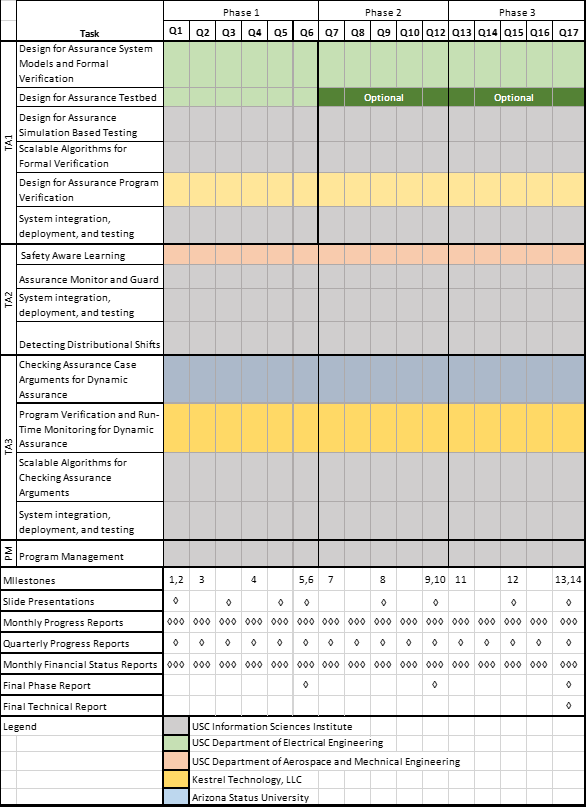
\includegraphics[width=.95\textwidth]{figs/Safeguard_Schedule_V6}
\end{center}
\vspace{-.2in}\caption{Project schedule along with a summary of milestones.  The legend maps task color to organization primary responsible for the task. } 
\label{fig:sandm}
\end{figure}
 

% \section{Level of Effort by Task \textcolor{red}{[Mike/Lisa - 1 pages]}}

% \textcolor{blue}{
% \begin{itemize}
% \item Will be a separate spreadsheet
% \item
% \end{itemize}
% }

\section*{Appendix A: Team Members and Other Information}
\addcontentsline{toc}{section}{Appendix A: Team Members and Other Information}

\baades{This section is mandatory and must include all of the following
components. If a particular subsection is not applicable, state “NONE”.}

\vspace{1ex}

\noindent
\textbf{Team Member Identification}:

\vspace{1ex}

\baades{Provide a list of all team members including the
prime, subcontractor(s), and consultant(s), as applicable. Identify specifically
whether any are a non-US organization or individual, FFRDC and/or Government
entity.}

\begin{centering}

%\small
\begin{tabular}{|p{1.8in}|p{1in}|p{1.1in}|p{0.7in}|p{0.8in}|p{0.7in}|}
\hline
 \textbf{Name} &  \textbf{Role} & \textbf{Organization} & \textbf{Non-US Org?}  & \textbf{Non-US Ind?} &  \textbf{FFRDC or Gov} \\
 \hline
Craig A. Knoblock & Prime & USC & N & N & N\\ \hline
Michael Orosz & Prime & USC & N &  N & N \\ \hline
Satish Thittamaranahalli & Prime & USC & N &  Y & N \\ \hline
Ryan Goodfellow & Prime & USC & N &  N & N \\ \hline
Anoop Kumar & Prime & USC & N & N & N \\ \hline
Satyandra Gupta & Prime & USC & N & N & N \\ \hline
Pierluigi Nuzzo & Prime & USC & N & Y & N \\ \hline
Petros Ioannou & Prime & USC & N & N & N \\ \hline
Chitta Baral & Subcontractor & ASU & N & N & N \\ \hline
Matt Barry & Subcontractor & Kestrel Technology & N & N & N \\ \hline
Douglas Smith & Subcontractor & Kestrel Technology & N & N & N \\ \hline
Henny Sipma & Subcontractor & Kestrel Technology & N & Y & N \\ \hline
\end{tabular} 
\end{centering}

\vspace{1ex}

\noindent
\textbf{Government or FFRDC Team Member Proof of Eligibility to Propose}: NONE

\baades {If
none of the team member organizations (prime or subcontractor) are a
Government entity or FFRDC, state “NONE”.}

\vspace{1ex}

\noindent
\textbf{Government or FFRDC Team Member Statement of Unique Capability}: NONE

\vspace{1ex}

\noindent
\textbf{Organizational Conflict of Interest Affirmations and Disclosure}: NONE

\vspace{1ex}

\noindent
\textbf{Intellectual Property (IP)}: 
\baades {
If no IP restrictions are intended, state “NONE”.
The Government will assume unlimited rights to all IP not explicitly identified as
having less than unlimited rights in the proposal.
For all technical data or computer software that will be furnished to the
Government with other than unlimited rights, provide (per Section VI.B.1) a list
describing all proprietary claims to results, prototypes, deliverables or systems
supporting and/or necessary for the use of the research, results, prototypes
and/or deliverables. Provide documentation proving ownership or possession of
appropriate licensing rights to all patented inventions (or inventions for which a
patent application has been filed) to be used for the proposed project.
}
\begin{centering}

%\small
\begin{tabular}{|p{2.1in}|p{1.2in}|p{1.4in}|p{2in}|}
\hline
\multicolumn{4}{|c|}{COMMERCIAL ITEMS }\\ \hline 
 \textbf{Technical Data, Computer Software To be Furnished With Restrictions} &  \textbf{Basis for Assertion} & \textbf{Asserted Rights Category} & \textbf{Name of Person Asserting Restrictions}  \\  \hline
KT Advance & Developed with mixed funding. & Restricted & David Kulich, Contracts Manager, Kestrel technology, LLC.\\ \hline
\end{tabular} 
\end{centering}

\vspace{1ex}

\noindent
\textbf{Human Subjects Research (HSR)}: NONE

\vspace{1ex}

\noindent
\textbf{Animal Use}: NONE

\vspace{1ex}

\noindent
\textbf{Representations Regarding Unpaid Delinquent Tax Liability or a Felony
Conviction under Any Federal Law}: 
%NONE

\begin{enumerate}
\item
The proposer is  not a corporation that has any unpaid Federal tax liability that has been assessed, for which all judicial and administrative remedies have been exhausted or have lapsed, and that is not being paid in a timely manner pursuant to an agreement with the authority responsible for collecting the tax liability,
\item
The proposer is not a corporation that was convicted of a felony criminal violation under a Federal law within the preceding 24 months.
\end{enumerate}

\vspace{1ex}

\noindent
\textbf{Cost Accounting Standards (CAS) Notices and Certification}:
\baades{
For any proposer who submits a proposal which, if accepted, will result in a CAS-compliant
contract, must include a Disclosure Statement as required by 48 CFR
9903.202. The disclosure forms may be found at
http://www.whitehouse.gov/omb/procurement\_casb
If this section is not applicable, state “NONE”. For further information regarding
this subject, please see www.darpa.mil/work-with-us/additional-baa.
}
NONE


%\section{Appendix B \textcolor{red}{[No Page Count]}}

\section{References}
\bibliographystyle{acm} 
\bibliography{TA3/ta3,TA2/ta2,TA1/ta1}
\end{document}
%%\documentclass[a4paper]{article}
%\documentclass[12pt]{article}
\documentclass[12pt]{dod-blank}

%% Language and font encodings
\usepackage[english]{babel}
\usepackage[utf8x]{inputenc}
\usepackage[T1]{fontenc}

%% Sets page size and margins
%%\usepackage[a4paper,top=3cm,bottom=2cm,left=3cm,right=3cm,marginparwidth=1.75cm]{geometry}
%\usepackage[top=1in, bottom=1in, left=1in, right=1in]{geometry}



%% Useful packages
\usepackage{amsmath}
\usepackage{graphicx}
  \graphicspath{{.}{./image/}}
  \DeclareGraphicsExtensions{.png,.jpg} 
\usepackage[colorinlistoftodos]{todonotes}
\usepackage[colorlinks=true, allcolors=blue]{hyperref}
\usepackage{tabularx}
\usepackage{multirow}
\usepackage{tabulary}
\usepackage{float}
\usepackage{wrapfig}
\usepackage[export]{adjustbox}
\usepackage{comment}
\usepackage{tabularx}
\usepackage{multirow}
\usepackage{tabulary}
\usepackage{enumitem}

\usepackage{listings}
\usepackage{color}
\usepackage{array}
\usepackage{subcaption}
\usepackage{xcolor}




\renewcommand{\textfraction}{0}
\renewcommand{\topfraction}{1.0}
\renewcommand{\bottomfraction}{1.0}

\usepackage{longtable}
%% macros
\newif\iffinal
\finaltrue
\iffinal
  
    \newcommand\baareq[1]{}
    \newcommand\baades[1]{}
 
 
\else
    \definecolor{darkgreen}{rgb}{0,0.4,0}
    \definecolor{darkcyan}{rgb}{0,0.4,0.4}
    \definecolor{darkblue}{rgb}{0,0,0.5}
    
    \newcommand\baareq[1]{{\color{darkcyan}[\textbf{Requirement:} #1]}}
    \newcommand\baades[1]{{\color{darkcyan}[\textbf{Description:} #1]}}
 
\fi




\def\naive{na\"{\i}ve}



\lstset{ 
  backgroundcolor=\color{white},   % choose the background color; you must add \usepackage{color} or \usepackage{xcolor}
  basicstyle=\footnotesize\ttfamily,            % the size of the fonts that are used for the code
  breakatwhitespace=false,         % sets if automatic breaks should only happen at whitespace
  breaklines=true,                 % sets automatic line breaking
  captionpos=b,                    % sets the caption-position to bottom
  commentstyle=\color{mygreen},    % comment style
  % deletekeywords={...},            % if you want to delete keywords from the given language
  escapeinside={\%*}{*)},          % if you want to add LaTeX within your code
  extendedchars=true,              % lets you use non-ASCII characters; for 8-bits encodings only, does not work with UTF-8
  frame=single,	                   % adds a frame around the code
  keepspaces=false,                 % keeps spaces in text, useful for keeping indentation of code (possibly needs columns=flexible)
  keywordstyle=\color{blue}\bfseries\underbar,       % keyword style
  language=Prolog,                 % the language of the code
  % morekeywords={if,and},        % if you want to add more keywords to the set
  numbers=none,                    % where to put the line-numbers; possible values are (none, left, right)
  numbersep=5pt,                   % how far the line-numbers are from the code
  numberstyle=\tiny\color{mygray}, % the style that is used for the line-numbers
  rulecolor=\color{black},         % if not set, the frame-color may be changed on line-breaks within not-black text
  showspaces=false,                % show spaces everywhere adding particular underscores; it overrides 'showstringspaces'
  showstringspaces=false,          % underline spaces within strings only
  showtabs=false,                  % show tabs within strings adding particular underscores
  stepnumber=2,                    % the step between two line-numbers. If it's 1, each line will be numbered
  stringstyle=\color{mymauve},     % string literal style
  tabsize=2,	                   % sets default tabsize to 2 spaces
  title=\lstname                   % show the filename of files included with \lstinputlisting; also try caption instead of title
}

% apply trick for additional keywords for our AC DSL
\lstset{
	emph={for, if, and, or},
    emphstyle={\color{blue}\bfseries\underbar}
}




\title{DARPA Assured Autonomy}
\author{Technical Volume- \textcolor{red}{Thirty-Eight (38) pages max}}

\begin{document}
\pagenumbering{roman}
 
\begin{center}
\large{\textbf{Volume 1: Technical and Management Proposal}}
\end{center}
\textbf{BAA Number:} DARPA-HR001117S0045 \\
\textbf{Technical Area:} TA1, TA2, and TA3 \\
\textbf{Proposal Title:} Assured Autonomy for Learning Enabled Vehicles (Safeguard) \\
\textbf{Lead Institution:} University of Southern California \\
\textbf{Type of organization: } “OTHER EDUCATIONAL” \\

\begin{tabularx}{\linewidth}{XX}

 \textbf{Technical Point of Contact} &  \textbf{Administrative Point of Contact }   \\
Dr.\ Craig A. Knoblock  & Sapphire Masterson  \\ 
USC Information Sciences Institute & USC Dept. of Contracts \& Grants \\
4676 Admiralty Way, Suite 1001 & 4676 Admiralty Way, Suite 1001 \\
Marina del Rey, CA 90292 & Marina del Rey, CA 90292 \\
Tel: 310-448-8786 &  Tel: (310) 448-9161 \\
E-mail: knoblock@isi.edu  & E-mail: sapphirm@usc.edu \\
\end{tabularx}
\\
\\
\textbf{Award instrument requested:}  Procurement Contract, Cost-Reimbursement, No Fee
\\
\\
\textbf{Total amount of the proposed effort:} \$ ...\\
Phase I: \$ ... \\
Phase II: \$ ... \\
Phase III: \$ ... \\
\\
\textbf{Place(s) of performance:} USC, Marina del Rey, CA; Los Angeles, CA;  Tempe, AZ; Palo Alto, CA \\
\textbf{Period(s) of performance:} 04/02/2018 - 03/31/2022     \\
\\
\textbf{Other team members:} \\
\begin{tabularx}{\linewidth}{XX}
Kestrel Technology  & Arizona State University \\
(small business) & (Other Educational)\\
POC: Matthew Barry & POC: Chitta Baral\\
3260 Hillview Avenue & Department of Computer Science and Engr. \\
Palo Alto, CA 94304 & Ira A. Fulton School of Engineering \\ 
phone: (832)205-4876 & Arizona State University\\ 
mrbarry@kestreltechnology.com & Brickyard Suite 572, 699 S. Mill Avenue \\
& Tempe, AZ 85281-8809, U.S.A.\\
& email: chitta@asu.edu\\
\end{tabularx}
\\
\textbf{Proposal validity period: } 180 days\\
\\
\textbf{Data Universal Numbering System (DUNS) number: } 072933393\\
\textbf{Taxpayer identification number:} 95-1642394\\
\textbf{Commercial and Government Entity (CAGE) code:} 1B729 Marina del Rey, CA\\
\textbf{Proposer’s reference number (if any):}  4409-0\\

\newpage
\section{Table of Contents}
\tableofcontents

\newpage
\pagenumbering{arabic}
\section{Executive Summary}
As we rapidly move into a world where machine learning plays a central role in realizing autonomous systems, it is becoming increasingly important to develop techniques that assure that these systems will operate safely and perform as expected. Current approaches are limited to providing assurance for systems with limited or no  learning capabilities. In this context, DARPA's Assured Autonomy BAA seeks to \emph{develop rigorous design and analysis technologies for continual assurance of learning-enabled autonomous systems}. USC in collaboration with Kestrel Technology and ASU is pleased to submit a comprehensive TA1, TA2, and TA3 proposal entitled \emph{``Assured Autonomy for Learning Enabled Vehicles (Safeguard).''} We plan to provide an end-to-end solution to support autonomous systems with learning-enabled components, ranging from design technologies for assurance, to assurance monitoring and control techniques, to representation and online evaluation of assurance cases. We have assembled a strong team of experts that cover the range of technologies that are required to create such an end-to-end system. If successful, the project will provide the technologies for building the next-generation of learning-enabled autonomous systems.  The entire project will take four years and cost \textcolor{red}{\$??}, with an initial version completed at the end of Phase I and successive versions with additional capabilities and improved scalability at the end of Phase II and Phase III.  

In the remainder of this section, we first introduce an  unmanned surface vehicle scenario that will be used throughout the proposal to describe the approach.  Next, we describe our approach to design, monitoring, and dynamic assurance. Finally, we introduce the team involved in the project. 

\textbf{Motivating Scenario.} Consider an autonomous unmanned surface vehicle (USV) guarding a valuable asset in the ocean when an unknown vehicle  approaches the security perimeter, under challenging weather conditions. In this scenario, the USV is required to approach the intruding vehicle, issue a warning signal, and escort it to a safe distance from the controlled area. However, as the USV has no a priori knowledge of its external environment behaviors (e.g., water depth, waves, wind, current, visibility), pre-computing a feasible trajectory, let alone optimal, becomes a non-trivial problem. For trajectory planning, the USV must continuously perform the following tasks:
\begin{itemize}[itemsep=0pt,leftmargin=*]
 \item Sense the current state of the surrounding environment (e.g., water depth, waves, wind, current, visibility) and estimate its own maneuverability constraints (e.g., braking distance, available acceleration, maximum velocity, turning radius, turning rate, safety distance) based on the state of the environment;      
\item Sense the static obstacles in the sensor range and generate a traversability map;
\item Sense the moving obstacles and classify them;   
\item Predict future trajectories of moving obstacles; 
\item Determine if any of the COLREGS \cite{commandant1999international} rules will be in effect with respect to one or more of the nearby vessels and identify the vessels with the right of way.    
\end{itemize}
The above information will be used by the trajectory planner to compute an initial trajectory, which will be continuously refined as the USV gathers additional information.
% It is not possible for the USV to be tested in every possible environment. 
The USV will use learning enabled components to take  decisions as it encounters new situations, such as  
\begin{itemize}[itemsep=0pt,leftmargin=*]
\item Classifiers to identify moving obstacles based on physical appearance and motion signatures,
\item Algorithms to estimate the sensor capabilities in adverse weather conditions,   
\item Algorithms to accurately estimate uncertainty in the environment, 
\item Classifiers to generate traversability maps,
\item Prediction of external vessel behaviors based on motion histories, 
\item Reinforcement learning  to ensure COLREGS compliance of maneuvers,  
\item Algorithms to learning pursuit behaviors.  
\end{itemize}
Learning enabled components will interact with each other in complex ways, where a misclassification error in one component may eventually compromise the entire mission.   
% We will need to make sure that each learning enabled components has a run-time monitor that will ensure that the assumptions made by the learning-enabled component remain valid and prevent erroneous learning. 
% For example, if the vehicle is exhibiting significant error in trajectory tracking, then simply downgrading the trajectory tracking error value may not be a good option.  The failure of prediction of trajectory tracking error might be due to the presence of a significant wake caused by a nearby vessel. The presence of the nearby vessel can be used to explain the degradation in trajectory tracking performance. As the vessel moves away, we can expect the trajectory tracking performance to return to the predicted level.  
While exhaustive validation of learning-enabled cyber-physical systems (LE-CPSs) is a prohibitive task~\cite{Kalra16},
their complexity, heterogeneity, and highly dynamic nature
make it challenging to even leverage existing model-based development techniques to effectively assess system correctness 
% dependability, 
at design time or enforce it at runtime.

\textbf{Design for Assurance.} Safeguard uses a platform-based design approach~\cite{Nuzzo15b} to organize the design process for a LE-CPS and to build assurance cases. Composite models are developed at several levels of abstraction,
from top-level system requirements and safety constraints down to the
implementation level.  Intermediate levels add detail to the levels
above.  The different levels are connected by refinement mappings that
allow properties established at one level to be preserved at the next
level (see Figures~\ref{fig:methodology} and~\ref{fig:assurance}).

Contracts are used to formally specify components and composite models
in terms of (1) Assumptions -- the assumed behaviors of the
environment and the behaviors of other components, and (2) Guarantees
-- the behavior properties that a model guarantees if it operates in a
context that satisfies its assumptions.  A calculus of contracts
allows horizontal composition of contracts to generate contracts for
composite models.  Vertical contracts are used to specify the mapping
or refinement relation between models at different levels of
abstraction.  The system design process starts with a high-level
contract that expresses overall system assumptions and requirements.
Subsequent levels express models with increasing detail until the
lowest level expresses the system in terms of hardware components and
their software controllers.

The assurance case for a CPS arises from the horizontal and vertical
structure of the design in several ways.  The components used within a
particular level are either (1) synthesized using
correct-by-construction design tools together with proofs, (2) derived
statically or dynamically using safety-aware machine-learning
techniques, (3) written manually and verified by analysis tools, or
(4) written manually and validated by extensive testing.  The
assurance case for the whole reflects its compositional structure.  We
anticipate that well-specified contracts together with the calculus of
contracts will eliminate well-known problems with unexpected emergent
behaviors in CPS systems.

The assurance case for the lowest-layer design arises from both the
intra-level assurance and from properties and their proofs that are
preserved under the refinement mapping from the top-level
requirements.  The refinement mappings between model layers will be
constructed using a variety of techniques.  A contract at an abstract
level can be mapped to a component or refined contract by (1)
retrieval of pre-verified components from a platform library, (2)
synthesis using correct-by-construction design and optimization tools,
or (3) manual coding to satisfy a contract.  The mapping of a
composite model will be composed from the mappings of its constituent
components or contracts.  When a composite model cannot be mapped
compositionally to the next level, it will be generated using
correct-by-construction design and optimization tools.

\textbf{Assurance Monitoring and Control.}
We provide an integrated framework for safety-aware learning, assurance monitoring and control, detecting distribution shifts. Three major components offer an efficient TA2 architecture as well as interfaces with TA1 and TA3, that is, (a) safety-aware learning and planning, (b) assurance monitors for guarding architectural and safety constraints; and (c) distribution shift detection.

We will develop a new learning-enabled online decision-making framework that allows opportunistically composing a sequence of actions (maneuvers) to reduce uncertainty in the system capability model without suspending the progress toward the mission goals or compromising safety. Each candidate action is evaluated based on three criteria: (1) the risk of violating a safety constraint using the current uncertainties in the parameter estimates; (2) its relevance to the mission goals; (3)  its expected information gain, i.e., reduction in uncertainty, with respect to the parameter estimates. These evaluations are combined to produce a cumulative mission utility value for each action that drives our learning-enabled decision-making framework. The problem of generating and evaluating sequences of actions can be posed in several way. For example, it can be solved using a branch-and-bound search method like Anytime A*, or formulated with the finite-horizon Markov Decision Process (MDP) framework. We will develop new scalable search strategies to solve this problem efficiently, by potentially evaluating a recent method developed at USC, called FastMap, that can significantly improve the execution time. 

We will develop monitors for architectural and safety constraints. 
% While these constraints can be checked over and over again as sensor information flow in, this naive strategy accounts for a lot of computational overhead. 
To achieve scalability and decrease the overhead, we propose the application of a technique that we currently use in DARPA's RSPACE program, which leverages a physical model of the vehicles dynamics and its interactions with the environment to efficiently determine the readout frequency. We propose two  extensions of this basic idea. First, we will use the theory of Variable Elimination to prioritize which variables to monitor, e.g., controllable, versus uncontrollable, adversarially controlled, or unobservable variables. Second, we invoke the dynamic assessment of assurance cases only when needed. This  decreases the number of times dynamic assessment of assurance cases is initiated as well as the communication bandwidth between the TA2 and TA3 components.

Finally, we will identify a distribution shift by combining statistical and machine learning techniques to differentiate between environmental and sensor changes. We will exploit a categorization of the shifts based on their cause and duration as well as extend our earlier work on detecting and mitigating sensor failures for all types of monitored variables.  

\textbf{Dynamic Assurance:} The Safeguard {\em design for assurance\/} activity takes a systems-theoretic stance toward safety.  Consequently, it presumes that safety is an emergent property of the system, and that hazards can present themselves through unintended interactions and performance violations in addition to causal events such as component failures.  Our design approach includes consideration of intent as well as hazard analysis and mitigation.  The artifacts from these activities populate contracts and assumptions for the dynamic assurance case.  
We thus build safety into the product by working at a systems-level viewpoint, using lexicon and design patterns familiar to both hardware and software engineers; safety is an emergent property of the system, not an afterthought.  
As system behavior evolves during runtime owing to learning, threats, degradation, or some other factor, the dynamic assurance case identifies whether the safety constraints continue to be satisfied.  If not, it provides notifications or issues recovery instructions directly from a lookup table.

Our implementation of the dynamic assurance case employs a declarative knowledge base inference engine and a domain-specific language tailored to our approach.  We have used them successfully for assurance case tool sets and arguments, and will extend them to reason about uncertainty and learning.  Our approach to achieve scalability is to specialize solvers toward modularity and to take advantage of domain knowledge.  Specifically, we will develop answer set programming techniques for context-dependent learning for reasoning about the learning-enabled components as well as learning assurance rules.  We will develop new formalisms for uncertainty to include causality, using weights for computing probabilities, and probabilistic non-monotonicity.  To achieve scaling objectives we will implement specializations using modularity, weighted CSPs, and message passing. 

% The system safety constraints revealed from that design become the key elements of our dynamic assurance case.  Our verification tools ensure the constraints are relevant, identifiable, and their implementation and effect observable.  

\textbf{Team.} We have assembled a team that is exceptionally well-qualified to build the proposed Safeguard system.  The team will be led by Dr.\ Craig Knoblock, the Principal Investigator for the effort, who currently leads the Intelligent Systems Division at the Information Sciences Institute.  He has led many large DARPA and IARPA projects over the years and has a strong track record in conducting leading edge research and then transitioning the technology to commercial use.  He will be supported by Dr.\ Michael Orosz as the Project Manager, who also has  experience in managing large research projects and on autonomous systems.  The TA1 team will be led by Dr.\ Pierluigi Nuzzo, who is an expert in embedded system design methodologies and the  application of formal methods to cyber-physical systems.  The TA1 team also includes Dr.\ Doug Smith, who has spent many years working on scalable correct-by-construction techniques and Dr.\ Henny Sipma, who has significant experience in applying program verification methods to real-world problems.  The TA1 team also includes Ryan Goodfellow, who has done a large amount of work on simulation-based testing.  The TA2 team will be led by Dr.\ Knoblock who has worked on topics related to both monitoring and detecting distribution changes.  He will be supported by Dr.\ Satyandra Gupta, who is an expert on autonomous surface vehicles as well as on safety-aware learning. He will also be supported by Drs.\ Anoop Kumar and Satish Thittamaranahalli, who have also previously worked on efficient methods for execution monitoring.  The TA3 team will be lead by Dr.\ Matthew Barry, who has experience in creating the technologies for assurance cases.  He will be supported by Dr.\ Chitta Baral, who is an expert on ASP solvers and by Dr.\ Thittamaranahalli who is an expert on SAT solvers, both of which will be applied to provide scalable assurance case reasoning.  Finally, Dr.\ Petros Ioannou, who is an expert on control systems for autonomous vehicles will provide an autonomous vehicle platform, which will form the focus of our work until the TA4 teams provide additional vehicle platforms for development.  

\newpage
\section{Innovative Claims and Deliverables}

In this project we will develop and build an end-to-end system for assured autonomy.  This section describes the key innovations by technical area and then the overall deliverables of the project.

\paragraph{Design for Assurance}

\begin{itemize}[itemsep=0pt,leftmargin=*]
\item We address the LE-CPS design challenges via a holistic approach that can contextually generate design artifacts and assurance cases. We develop a compositional, contract-based modeling framework, methods, and tools to support the design process from system-level requirement capture,  formalization, and analysis, to the generation, testing, and continual monitoring of software and hardware artifacts in feedback loop with a physical process.

\item We develop compositional abstractions and interfaces (vertical contracts) that can  bridge heterogeneous formalisms and heterogeneous decomposition architectures to make system analysis and synthesis tractable, consistently combine different verification and synthesis methods at design time, and provide seamless support for dynamic assurance at run time. %We aim to quantitatively capture the confidence in the satisfaction of requirements under uncertain or unknown conditions, and resilience properties of  systems at different abstraction levels, to enable trade-off evaluation between resilience, performance, and cost.

\item We develop a unifying framework and efficient algorithms to reason about the combination of discrete and continuous dynamics and constraints in the presence of uncertainties in LE-CPS using a satisfiability modulo convex approach~\cite{Shoukry2017} for contract-based system verification and scalable trajectory planning.  

\item We provide an environment for high-fidelity CPS testing, in which production-ready software, e.g.,  safety-critical learning and control, may be deployed and tested 
% by extending the Cypress testbed environment \cite{Goodfellow2015Cypress:Systems} 
with time dilation facilities, so that it synchronizes with a physical simulation that is not necessarily running in real time, while still having the perception of real time.

\item We 
% These facilities allow a cyber system to be  
propose an approach for unanticipated behavior space identification and test coverage maximization which leverages results from the theory of differential algebraic equation (DAE)~\cite{Berger2013ControllabilitySurvey,Ilchmann2005ATheory,BergerOnSystems,Lamour2013} 
to prune the behavior search space and identify smaller regions of interest for efficient simulation-based testing. 
% We then compute the intersection of these two behavior spaces and restrict our simulation based testing search space to this subspace.
\end{itemize}

\paragraph{Assurance Monitoring and Control}

\begin{itemize}[itemsep=0pt,leftmargin=*]
\item 
%We integrate safety-aware learning into the overall decision making problem. The goal is to maximize mission utility without violating the safety constraints. 
Our safety-aware learning framework enables the system to opportunistically select and execute actions to assist the learning-enabled component in reducing model uncertainty without compromising safety or deviating from the mission goals. The value of uncertainty reduction is explicitly incorporated in the optimization process for selecting the best action.  
\item For safety-aware learning, we propose the idea of preprocessing the search space of the problem domain before queries and observations come in. With such a linear-time preprocessing phase, the performance of search and optimization algorithms can be significantly boosted. For example, in regular A* search, the intensional or extensional search space can be preprocessed in near-linear time to yield an embedding of each state as a point in Euclidean space~\cite{cujakk}. Then, when the query comes in, A* search can make use of these Euclidean distances as heuristic distances between two states to yield order-of-magnitude speedups. 
%In Anytime A* for safety-aware learning and planning, this leads to a significantly better quality of actions chosen within a time limit, and in the MDP framework, the same ideas can be used to improve the convergence of Bellman updates for safety-aware Reinforcement Learning.
\item As massive amounts of sensor information flow in, it is imperative for us to efficiently process this information for monitoring architectural and safety constraints. Building on our past work on similar tasks, we propose novel technologies for efficiently monitoring constraints. These algorithms can yield an exponential reduction in the amount of sensor data that needs to be processed. Doing this also reduces the message complexities between the various modules. %We also propose to use the theory of Variable Elimination (VE) to monitor constraints with uncontrollable, adversarially controlled, and/or unobservable variables. VE yields a substrate constraint to monitor that characterizes a dominant strategy of the controllable variables over the uncontrollable, adversarially controlled, and/or unobservable variables.
\item We will develop techniques to identify  distributional shifts and determine the underlying cause (e.g., change in environment, sensor failure,   etc.), as well as strategies for handling the various distributional shifts.   Notably, we propose to build on our past work and use compact representations to exploit historical data to identify distributional shifts.
\end{itemize}

\paragraph{Dynamic Assurance}

\begin{itemize}[itemsep=0pt,leftmargin=*]

\item We demonstrate the integration of dynamic assurance for safety-critical learning-enabled dynamic systems in which evolutionary behaviors are expected and tolerated as a property of the functionality.   The impact will be consequential contributions safety-critical dynamic systems in which evolutionary behaviors are expected and tolerated as portion of the functionality.   
\item We implement dynamic assurance by combining features of system safety, formal methods, logic programming, uncertain reasoning, and domain-specific languages.  We populate assurance case arguments at several levels of modeling and implementation abstraction, using the analysis results to produce design-time evidence supporting assurance claims.  
%We provide automated reasoning about the assurance case itself to produce verification, consistency, and completeness results for the argument.  Dynamic assurance results then yield trusted explanations of whether safety constraints and assumptions and other contracts still hold during the collection of runtime evidence from monitors. 
\item We develop and demonstrate ASP formalisms crucial to applications in dynamic assurance. We demonstrate the suitability of the technology especially for assurance case arguments owing to the improved legibility, consistency and completeness checks, handling of uncertain and default reasoning, and scalability.  
%We will produce modularized solvers for enhanced performance based on recent algorithmic developments in exploiting structure, kernelization, and message passing. We provide a formalism to enable learning of assurance rules. 
We provide a novel approach to handling uncertainty that provides the ability to do causal and counter-factual reasoning as well as probabilistic non-monotonicity.  Overcoming limitations of traditional inductive logic techniques, we develop a novel iterative and incremental approach based on context dependent learning. 
\end{itemize}

\paragraph{Deliverables}
During the course of this project, we will build and deliver a fully-operational system that covers all three of the technical areas.  The detailed capabilities of this system are described in the individual technical sections.  The resulting system will be available as open source under a permissive license, which will allow other organizations to use the work, extend it in new directions, and even commercialize the software.  Kestrel Technology has significant experience in this space and has built and applied these types of technologies to a variety of real world tasks.  Kestrel is ideally suited to pursue commercial uses of this technology and the permissive license will facilitate exploring these opportunities since there will be no need to negotiate intellectual property rights.  

\newpage
\section{Technical Plan}
%%\documentclass[a4paper]{article}
%\documentclass[12pt]{article}
\documentclass[12pt]{dod-blank}

%% Language and font encodings
\usepackage[english]{babel}
\usepackage[utf8x]{inputenc}
\usepackage[T1]{fontenc}

%% Sets page size and margins
%%\usepackage[a4paper,top=3cm,bottom=2cm,left=3cm,right=3cm,marginparwidth=1.75cm]{geometry}
%\usepackage[top=1in, bottom=1in, left=1in, right=1in]{geometry}



%% Useful packages
\usepackage{amsmath}
\usepackage{graphicx}
  \graphicspath{{.}{./image/}}
  \DeclareGraphicsExtensions{.png,.jpg} 
\usepackage[colorinlistoftodos]{todonotes}
\usepackage[colorlinks=true, allcolors=blue]{hyperref}
\usepackage{tabularx}
\usepackage{multirow}
\usepackage{tabulary}
\usepackage{float}
\usepackage{wrapfig}
\usepackage[export]{adjustbox}
\usepackage{comment}
\usepackage{tabularx}
\usepackage{multirow}
\usepackage{tabulary}
\usepackage{enumitem}

\usepackage{listings}
\usepackage{color}
\usepackage{array}
\usepackage{subcaption}
\usepackage{xcolor}




\renewcommand{\textfraction}{0}
\renewcommand{\topfraction}{1.0}
\renewcommand{\bottomfraction}{1.0}

\usepackage{longtable}
%% macros
\newif\iffinal
\finaltrue
\iffinal
  
    \newcommand\baareq[1]{}
    \newcommand\baades[1]{}
 
 
\else
    \definecolor{darkgreen}{rgb}{0,0.4,0}
    \definecolor{darkcyan}{rgb}{0,0.4,0.4}
    \definecolor{darkblue}{rgb}{0,0,0.5}
    
    \newcommand\baareq[1]{{\color{darkcyan}[\textbf{Requirement:} #1]}}
    \newcommand\baades[1]{{\color{darkcyan}[\textbf{Description:} #1]}}
 
\fi




\def\naive{na\"{\i}ve}



\lstset{ 
  backgroundcolor=\color{white},   % choose the background color; you must add \usepackage{color} or \usepackage{xcolor}
  basicstyle=\footnotesize\ttfamily,            % the size of the fonts that are used for the code
  breakatwhitespace=false,         % sets if automatic breaks should only happen at whitespace
  breaklines=true,                 % sets automatic line breaking
  captionpos=b,                    % sets the caption-position to bottom
  commentstyle=\color{mygreen},    % comment style
  % deletekeywords={...},            % if you want to delete keywords from the given language
  escapeinside={\%*}{*)},          % if you want to add LaTeX within your code
  extendedchars=true,              % lets you use non-ASCII characters; for 8-bits encodings only, does not work with UTF-8
  frame=single,	                   % adds a frame around the code
  keepspaces=false,                 % keeps spaces in text, useful for keeping indentation of code (possibly needs columns=flexible)
  keywordstyle=\color{blue}\bfseries\underbar,       % keyword style
  language=Prolog,                 % the language of the code
  % morekeywords={if,and},        % if you want to add more keywords to the set
  numbers=none,                    % where to put the line-numbers; possible values are (none, left, right)
  numbersep=5pt,                   % how far the line-numbers are from the code
  numberstyle=\tiny\color{mygray}, % the style that is used for the line-numbers
  rulecolor=\color{black},         % if not set, the frame-color may be changed on line-breaks within not-black text
  showspaces=false,                % show spaces everywhere adding particular underscores; it overrides 'showstringspaces'
  showstringspaces=false,          % underline spaces within strings only
  showtabs=false,                  % show tabs within strings adding particular underscores
  stepnumber=2,                    % the step between two line-numbers. If it's 1, each line will be numbered
  stringstyle=\color{mymauve},     % string literal style
  tabsize=2,	                   % sets default tabsize to 2 spaces
  title=\lstname                   % show the filename of files included with \lstinputlisting; also try caption instead of title
}

% apply trick for additional keywords for our AC DSL
\lstset{
	emph={for, if, and, or},
    emphstyle={\color{blue}\bfseries\underbar}
}




\title{DARPA Assured Autonomy}
\author{Technical Volume- \textcolor{red}{Thirty-Eight (38) pages max}}

\begin{document}
\pagenumbering{roman}
 
\begin{center}
\large{\textbf{Volume 1: Technical and Management Proposal}}
\end{center}
\textbf{BAA Number:} DARPA-HR001117S0045 \\
\textbf{Technical Area:} TA1, TA2, and TA3 \\
\textbf{Proposal Title:} Assured Autonomy for Learning Enabled Vehicles (Safeguard) \\
\textbf{Lead Institution:} University of Southern California \\
\textbf{Type of organization: } “OTHER EDUCATIONAL” \\

\begin{tabularx}{\linewidth}{XX}

 \textbf{Technical Point of Contact} &  \textbf{Administrative Point of Contact }   \\
Dr.\ Craig A. Knoblock  & Sapphire Masterson  \\ 
USC Information Sciences Institute & USC Dept. of Contracts \& Grants \\
4676 Admiralty Way, Suite 1001 & 4676 Admiralty Way, Suite 1001 \\
Marina del Rey, CA 90292 & Marina del Rey, CA 90292 \\
Tel: 310-448-8786 &  Tel: (310) 448-9161 \\
E-mail: knoblock@isi.edu  & E-mail: sapphirm@usc.edu \\
\end{tabularx}
\\
\\
\textbf{Award instrument requested:}  Procurement Contract, Cost-Reimbursement, No Fee
\\
\\
\textbf{Total amount of the proposed effort:} \$ ...\\
Phase I: \$ ... \\
Phase II: \$ ... \\
Phase III: \$ ... \\
\\
\textbf{Place(s) of performance:} USC, Marina del Rey, CA; Los Angeles, CA;  Tempe, AZ; Palo Alto, CA \\
\textbf{Period(s) of performance:} 04/02/2018 - 03/31/2022     \\
\\
\textbf{Other team members:} \\
\begin{tabularx}{\linewidth}{XX}
Kestrel Technology  & Arizona State University \\
(small business) & (Other Educational)\\
POC: Matthew Barry & POC: Chitta Baral\\
3260 Hillview Avenue & Department of Computer Science and Engr. \\
Palo Alto, CA 94304 & Ira A. Fulton School of Engineering \\ 
phone: (832)205-4876 & Arizona State University\\ 
mrbarry@kestreltechnology.com & Brickyard Suite 572, 699 S. Mill Avenue \\
& Tempe, AZ 85281-8809, U.S.A.\\
& email: chitta@asu.edu\\
\end{tabularx}
\\
\textbf{Proposal validity period: } 180 days\\
\\
\textbf{Data Universal Numbering System (DUNS) number: } 072933393\\
\textbf{Taxpayer identification number:} 95-1642394\\
\textbf{Commercial and Government Entity (CAGE) code:} 1B729 Marina del Rey, CA\\
\textbf{Proposer’s reference number (if any):}  4409-0\\

\newpage
\section{Table of Contents}
\tableofcontents

\newpage
\pagenumbering{arabic}
\section{Executive Summary}
As we rapidly move into a world where machine learning plays a central role in realizing autonomous systems, it is becoming increasingly important to develop techniques that assure that these systems will operate safely and perform as expected. Current approaches are limited to providing assurance for systems with limited or no  learning capabilities. In this context, DARPA's Assured Autonomy BAA seeks to \emph{develop rigorous design and analysis technologies for continual assurance of learning-enabled autonomous systems}. USC in collaboration with Kestrel Technology and ASU is pleased to submit a comprehensive TA1, TA2, and TA3 proposal entitled \emph{``Assured Autonomy for Learning Enabled Vehicles (Safeguard).''} We plan to provide an end-to-end solution to support autonomous systems with learning-enabled components, ranging from design technologies for assurance, to assurance monitoring and control techniques, to representation and online evaluation of assurance cases. We have assembled a strong team of experts that cover the range of technologies that are required to create such an end-to-end system. If successful, the project will provide the technologies for building the next-generation of learning-enabled autonomous systems.  The entire project will take four years and cost \textcolor{red}{\$??}, with an initial version completed at the end of Phase I and successive versions with additional capabilities and improved scalability at the end of Phase II and Phase III.  

In the remainder of this section, we first introduce an  unmanned surface vehicle scenario that will be used throughout the proposal to describe the approach.  Next, we describe our approach to design, monitoring, and dynamic assurance. Finally, we introduce the team involved in the project. 

\textbf{Motivating Scenario.} Consider an autonomous unmanned surface vehicle (USV) guarding a valuable asset in the ocean when an unknown vehicle  approaches the security perimeter, under challenging weather conditions. In this scenario, the USV is required to approach the intruding vehicle, issue a warning signal, and escort it to a safe distance from the controlled area. However, as the USV has no a priori knowledge of its external environment behaviors (e.g., water depth, waves, wind, current, visibility), pre-computing a feasible trajectory, let alone optimal, becomes a non-trivial problem. For trajectory planning, the USV must continuously perform the following tasks:
\begin{itemize}[itemsep=0pt,leftmargin=*]
 \item Sense the current state of the surrounding environment (e.g., water depth, waves, wind, current, visibility) and estimate its own maneuverability constraints (e.g., braking distance, available acceleration, maximum velocity, turning radius, turning rate, safety distance) based on the state of the environment;      
\item Sense the static obstacles in the sensor range and generate a traversability map;
\item Sense the moving obstacles and classify them;   
\item Predict future trajectories of moving obstacles; 
\item Determine if any of the COLREGS \cite{commandant1999international} rules will be in effect with respect to one or more of the nearby vessels and identify the vessels with the right of way.    
\end{itemize}
The above information will be used by the trajectory planner to compute an initial trajectory, which will be continuously refined as the USV gathers additional information.
% It is not possible for the USV to be tested in every possible environment. 
The USV will use learning enabled components to take  decisions as it encounters new situations, such as  
\begin{itemize}[itemsep=0pt,leftmargin=*]
\item Classifiers to identify moving obstacles based on physical appearance and motion signatures,
\item Algorithms to estimate the sensor capabilities in adverse weather conditions,   
\item Algorithms to accurately estimate uncertainty in the environment, 
\item Classifiers to generate traversability maps,
\item Prediction of external vessel behaviors based on motion histories, 
\item Reinforcement learning  to ensure COLREGS compliance of maneuvers,  
\item Algorithms to learning pursuit behaviors.  
\end{itemize}
Learning enabled components will interact with each other in complex ways, where a misclassification error in one component may eventually compromise the entire mission.   
% We will need to make sure that each learning enabled components has a run-time monitor that will ensure that the assumptions made by the learning-enabled component remain valid and prevent erroneous learning. 
% For example, if the vehicle is exhibiting significant error in trajectory tracking, then simply downgrading the trajectory tracking error value may not be a good option.  The failure of prediction of trajectory tracking error might be due to the presence of a significant wake caused by a nearby vessel. The presence of the nearby vessel can be used to explain the degradation in trajectory tracking performance. As the vessel moves away, we can expect the trajectory tracking performance to return to the predicted level.  
While exhaustive validation of learning-enabled cyber-physical systems (LE-CPSs) is a prohibitive task~\cite{Kalra16},
their complexity, heterogeneity, and highly dynamic nature
make it challenging to even leverage existing model-based development techniques to effectively assess system correctness 
% dependability, 
at design time or enforce it at runtime.

\textbf{Design for Assurance.} Safeguard uses a platform-based design approach~\cite{Nuzzo15b} to organize the design process for a LE-CPS and to build assurance cases. Composite models are developed at several levels of abstraction,
from top-level system requirements and safety constraints down to the
implementation level.  Intermediate levels add detail to the levels
above.  The different levels are connected by refinement mappings that
allow properties established at one level to be preserved at the next
level (see Figures~\ref{fig:methodology} and~\ref{fig:assurance}).

Contracts are used to formally specify components and composite models
in terms of (1) Assumptions -- the assumed behaviors of the
environment and the behaviors of other components, and (2) Guarantees
-- the behavior properties that a model guarantees if it operates in a
context that satisfies its assumptions.  A calculus of contracts
allows horizontal composition of contracts to generate contracts for
composite models.  Vertical contracts are used to specify the mapping
or refinement relation between models at different levels of
abstraction.  The system design process starts with a high-level
contract that expresses overall system assumptions and requirements.
Subsequent levels express models with increasing detail until the
lowest level expresses the system in terms of hardware components and
their software controllers.

The assurance case for a CPS arises from the horizontal and vertical
structure of the design in several ways.  The components used within a
particular level are either (1) synthesized using
correct-by-construction design tools together with proofs, (2) derived
statically or dynamically using safety-aware machine-learning
techniques, (3) written manually and verified by analysis tools, or
(4) written manually and validated by extensive testing.  The
assurance case for the whole reflects its compositional structure.  We
anticipate that well-specified contracts together with the calculus of
contracts will eliminate well-known problems with unexpected emergent
behaviors in CPS systems.

The assurance case for the lowest-layer design arises from both the
intra-level assurance and from properties and their proofs that are
preserved under the refinement mapping from the top-level
requirements.  The refinement mappings between model layers will be
constructed using a variety of techniques.  A contract at an abstract
level can be mapped to a component or refined contract by (1)
retrieval of pre-verified components from a platform library, (2)
synthesis using correct-by-construction design and optimization tools,
or (3) manual coding to satisfy a contract.  The mapping of a
composite model will be composed from the mappings of its constituent
components or contracts.  When a composite model cannot be mapped
compositionally to the next level, it will be generated using
correct-by-construction design and optimization tools.

\textbf{Assurance Monitoring and Control.}
We provide an integrated framework for safety-aware learning, assurance monitoring and control, detecting distribution shifts. Three major components offer an efficient TA2 architecture as well as interfaces with TA1 and TA3, that is, (a) safety-aware learning and planning, (b) assurance monitors for guarding architectural and safety constraints; and (c) distribution shift detection.

We will develop a new learning-enabled online decision-making framework that allows opportunistically composing a sequence of actions (maneuvers) to reduce uncertainty in the system capability model without suspending the progress toward the mission goals or compromising safety. Each candidate action is evaluated based on three criteria: (1) the risk of violating a safety constraint using the current uncertainties in the parameter estimates; (2) its relevance to the mission goals; (3)  its expected information gain, i.e., reduction in uncertainty, with respect to the parameter estimates. These evaluations are combined to produce a cumulative mission utility value for each action that drives our learning-enabled decision-making framework. The problem of generating and evaluating sequences of actions can be posed in several way. For example, it can be solved using a branch-and-bound search method like Anytime A*, or formulated with the finite-horizon Markov Decision Process (MDP) framework. We will develop new scalable search strategies to solve this problem efficiently, by potentially evaluating a recent method developed at USC, called FastMap, that can significantly improve the execution time. 

We will develop monitors for architectural and safety constraints. 
% While these constraints can be checked over and over again as sensor information flow in, this naive strategy accounts for a lot of computational overhead. 
To achieve scalability and decrease the overhead, we propose the application of a technique that we currently use in DARPA's RSPACE program, which leverages a physical model of the vehicles dynamics and its interactions with the environment to efficiently determine the readout frequency. We propose two  extensions of this basic idea. First, we will use the theory of Variable Elimination to prioritize which variables to monitor, e.g., controllable, versus uncontrollable, adversarially controlled, or unobservable variables. Second, we invoke the dynamic assessment of assurance cases only when needed. This  decreases the number of times dynamic assessment of assurance cases is initiated as well as the communication bandwidth between the TA2 and TA3 components.

Finally, we will identify a distribution shift by combining statistical and machine learning techniques to differentiate between environmental and sensor changes. We will exploit a categorization of the shifts based on their cause and duration as well as extend our earlier work on detecting and mitigating sensor failures for all types of monitored variables.  

\textbf{Dynamic Assurance:} The Safeguard {\em design for assurance\/} activity takes a systems-theoretic stance toward safety.  Consequently, it presumes that safety is an emergent property of the system, and that hazards can present themselves through unintended interactions and performance violations in addition to causal events such as component failures.  Our design approach includes consideration of intent as well as hazard analysis and mitigation.  The artifacts from these activities populate contracts and assumptions for the dynamic assurance case.  
We thus build safety into the product by working at a systems-level viewpoint, using lexicon and design patterns familiar to both hardware and software engineers; safety is an emergent property of the system, not an afterthought.  
As system behavior evolves during runtime owing to learning, threats, degradation, or some other factor, the dynamic assurance case identifies whether the safety constraints continue to be satisfied.  If not, it provides notifications or issues recovery instructions directly from a lookup table.

Our implementation of the dynamic assurance case employs a declarative knowledge base inference engine and a domain-specific language tailored to our approach.  We have used them successfully for assurance case tool sets and arguments, and will extend them to reason about uncertainty and learning.  Our approach to achieve scalability is to specialize solvers toward modularity and to take advantage of domain knowledge.  Specifically, we will develop answer set programming techniques for context-dependent learning for reasoning about the learning-enabled components as well as learning assurance rules.  We will develop new formalisms for uncertainty to include causality, using weights for computing probabilities, and probabilistic non-monotonicity.  To achieve scaling objectives we will implement specializations using modularity, weighted CSPs, and message passing. 

% The system safety constraints revealed from that design become the key elements of our dynamic assurance case.  Our verification tools ensure the constraints are relevant, identifiable, and their implementation and effect observable.  

\textbf{Team.} We have assembled a team that is exceptionally well-qualified to build the proposed Safeguard system.  The team will be led by Dr.\ Craig Knoblock, the Principal Investigator for the effort, who currently leads the Intelligent Systems Division at the Information Sciences Institute.  He has led many large DARPA and IARPA projects over the years and has a strong track record in conducting leading edge research and then transitioning the technology to commercial use.  He will be supported by Dr.\ Michael Orosz as the Project Manager, who also has  experience in managing large research projects and on autonomous systems.  The TA1 team will be led by Dr.\ Pierluigi Nuzzo, who is an expert in embedded system design methodologies and the  application of formal methods to cyber-physical systems.  The TA1 team also includes Dr.\ Doug Smith, who has spent many years working on scalable correct-by-construction techniques and Dr.\ Henny Sipma, who has significant experience in applying program verification methods to real-world problems.  The TA1 team also includes Ryan Goodfellow, who has done a large amount of work on simulation-based testing.  The TA2 team will be led by Dr.\ Knoblock who has worked on topics related to both monitoring and detecting distribution changes.  He will be supported by Dr.\ Satyandra Gupta, who is an expert on autonomous surface vehicles as well as on safety-aware learning. He will also be supported by Drs.\ Anoop Kumar and Satish Thittamaranahalli, who have also previously worked on efficient methods for execution monitoring.  The TA3 team will be lead by Dr.\ Matthew Barry, who has experience in creating the technologies for assurance cases.  He will be supported by Dr.\ Chitta Baral, who is an expert on ASP solvers and by Dr.\ Thittamaranahalli who is an expert on SAT solvers, both of which will be applied to provide scalable assurance case reasoning.  Finally, Dr.\ Petros Ioannou, who is an expert on control systems for autonomous vehicles will provide an autonomous vehicle platform, which will form the focus of our work until the TA4 teams provide additional vehicle platforms for development.  

\newpage
\section{Innovative Claims and Deliverables}

In this project we will develop and build an end-to-end system for assured autonomy.  This section describes the key innovations by technical area and then the overall deliverables of the project.

\paragraph{Design for Assurance}

\begin{itemize}[itemsep=0pt,leftmargin=*]
\item We address the LE-CPS design challenges via a holistic approach that can contextually generate design artifacts and assurance cases. We develop a compositional, contract-based modeling framework, methods, and tools to support the design process from system-level requirement capture,  formalization, and analysis, to the generation, testing, and continual monitoring of software and hardware artifacts in feedback loop with a physical process.

\item We develop compositional abstractions and interfaces (vertical contracts) that can  bridge heterogeneous formalisms and heterogeneous decomposition architectures to make system analysis and synthesis tractable, consistently combine different verification and synthesis methods at design time, and provide seamless support for dynamic assurance at run time. %We aim to quantitatively capture the confidence in the satisfaction of requirements under uncertain or unknown conditions, and resilience properties of  systems at different abstraction levels, to enable trade-off evaluation between resilience, performance, and cost.

\item We develop a unifying framework and efficient algorithms to reason about the combination of discrete and continuous dynamics and constraints in the presence of uncertainties in LE-CPS using a satisfiability modulo convex approach~\cite{Shoukry2017} for contract-based system verification and scalable trajectory planning.  

\item We provide an environment for high-fidelity CPS testing, in which production-ready software, e.g.,  safety-critical learning and control, may be deployed and tested 
% by extending the Cypress testbed environment \cite{Goodfellow2015Cypress:Systems} 
with time dilation facilities, so that it synchronizes with a physical simulation that is not necessarily running in real time, while still having the perception of real time.

\item We 
% These facilities allow a cyber system to be  
propose an approach for unanticipated behavior space identification and test coverage maximization which leverages results from the theory of differential algebraic equation (DAE)~\cite{Berger2013ControllabilitySurvey,Ilchmann2005ATheory,BergerOnSystems,Lamour2013} 
to prune the behavior search space and identify smaller regions of interest for efficient simulation-based testing. 
% We then compute the intersection of these two behavior spaces and restrict our simulation based testing search space to this subspace.
\end{itemize}

\paragraph{Assurance Monitoring and Control}

\begin{itemize}[itemsep=0pt,leftmargin=*]
\item 
%We integrate safety-aware learning into the overall decision making problem. The goal is to maximize mission utility without violating the safety constraints. 
Our safety-aware learning framework enables the system to opportunistically select and execute actions to assist the learning-enabled component in reducing model uncertainty without compromising safety or deviating from the mission goals. The value of uncertainty reduction is explicitly incorporated in the optimization process for selecting the best action.  
\item For safety-aware learning, we propose the idea of preprocessing the search space of the problem domain before queries and observations come in. With such a linear-time preprocessing phase, the performance of search and optimization algorithms can be significantly boosted. For example, in regular A* search, the intensional or extensional search space can be preprocessed in near-linear time to yield an embedding of each state as a point in Euclidean space~\cite{cujakk}. Then, when the query comes in, A* search can make use of these Euclidean distances as heuristic distances between two states to yield order-of-magnitude speedups. 
%In Anytime A* for safety-aware learning and planning, this leads to a significantly better quality of actions chosen within a time limit, and in the MDP framework, the same ideas can be used to improve the convergence of Bellman updates for safety-aware Reinforcement Learning.
\item As massive amounts of sensor information flow in, it is imperative for us to efficiently process this information for monitoring architectural and safety constraints. Building on our past work on similar tasks, we propose novel technologies for efficiently monitoring constraints. These algorithms can yield an exponential reduction in the amount of sensor data that needs to be processed. Doing this also reduces the message complexities between the various modules. %We also propose to use the theory of Variable Elimination (VE) to monitor constraints with uncontrollable, adversarially controlled, and/or unobservable variables. VE yields a substrate constraint to monitor that characterizes a dominant strategy of the controllable variables over the uncontrollable, adversarially controlled, and/or unobservable variables.
\item We will develop techniques to identify  distributional shifts and determine the underlying cause (e.g., change in environment, sensor failure,   etc.), as well as strategies for handling the various distributional shifts.   Notably, we propose to build on our past work and use compact representations to exploit historical data to identify distributional shifts.
\end{itemize}

\paragraph{Dynamic Assurance}

\begin{itemize}[itemsep=0pt,leftmargin=*]

\item We demonstrate the integration of dynamic assurance for safety-critical learning-enabled dynamic systems in which evolutionary behaviors are expected and tolerated as a property of the functionality.   The impact will be consequential contributions safety-critical dynamic systems in which evolutionary behaviors are expected and tolerated as portion of the functionality.   
\item We implement dynamic assurance by combining features of system safety, formal methods, logic programming, uncertain reasoning, and domain-specific languages.  We populate assurance case arguments at several levels of modeling and implementation abstraction, using the analysis results to produce design-time evidence supporting assurance claims.  
%We provide automated reasoning about the assurance case itself to produce verification, consistency, and completeness results for the argument.  Dynamic assurance results then yield trusted explanations of whether safety constraints and assumptions and other contracts still hold during the collection of runtime evidence from monitors. 
\item We develop and demonstrate ASP formalisms crucial to applications in dynamic assurance. We demonstrate the suitability of the technology especially for assurance case arguments owing to the improved legibility, consistency and completeness checks, handling of uncertain and default reasoning, and scalability.  
%We will produce modularized solvers for enhanced performance based on recent algorithmic developments in exploiting structure, kernelization, and message passing. We provide a formalism to enable learning of assurance rules. 
We provide a novel approach to handling uncertainty that provides the ability to do causal and counter-factual reasoning as well as probabilistic non-monotonicity.  Overcoming limitations of traditional inductive logic techniques, we develop a novel iterative and incremental approach based on context dependent learning. 
\end{itemize}

\paragraph{Deliverables}
During the course of this project, we will build and deliver a fully-operational system that covers all three of the technical areas.  The detailed capabilities of this system are described in the individual technical sections.  The resulting system will be available as open source under a permissive license, which will allow other organizations to use the work, extend it in new directions, and even commercialize the software.  Kestrel Technology has significant experience in this space and has built and applied these types of technologies to a variety of real world tasks.  Kestrel is ideally suited to pursue commercial uses of this technology and the permissive license will facilitate exploring these opportunities since there will be no need to negotiate intellectual property rights.  

\newpage
\section{Technical Plan}
%%\documentclass[a4paper]{article}
%\documentclass[12pt]{article}
\documentclass[12pt]{dod-blank}

%% Language and font encodings
\usepackage[english]{babel}
\usepackage[utf8x]{inputenc}
\usepackage[T1]{fontenc}

%% Sets page size and margins
%%\usepackage[a4paper,top=3cm,bottom=2cm,left=3cm,right=3cm,marginparwidth=1.75cm]{geometry}
%\usepackage[top=1in, bottom=1in, left=1in, right=1in]{geometry}



%% Useful packages
\usepackage{amsmath}
\usepackage{graphicx}
  \graphicspath{{.}{./image/}}
  \DeclareGraphicsExtensions{.png,.jpg} 
\usepackage[colorinlistoftodos]{todonotes}
\usepackage[colorlinks=true, allcolors=blue]{hyperref}
\usepackage{tabularx}
\usepackage{multirow}
\usepackage{tabulary}
\usepackage{float}
\usepackage{wrapfig}
\usepackage[export]{adjustbox}
\usepackage{comment}
\usepackage{tabularx}
\usepackage{multirow}
\usepackage{tabulary}
\usepackage{enumitem}

\usepackage{listings}
\usepackage{color}
\usepackage{array}
\usepackage{subcaption}
\usepackage{xcolor}




\renewcommand{\textfraction}{0}
\renewcommand{\topfraction}{1.0}
\renewcommand{\bottomfraction}{1.0}

\usepackage{longtable}
%% macros
\newif\iffinal
\finaltrue
\iffinal
  
    \newcommand\baareq[1]{}
    \newcommand\baades[1]{}
 
 
\else
    \definecolor{darkgreen}{rgb}{0,0.4,0}
    \definecolor{darkcyan}{rgb}{0,0.4,0.4}
    \definecolor{darkblue}{rgb}{0,0,0.5}
    
    \newcommand\baareq[1]{{\color{darkcyan}[\textbf{Requirement:} #1]}}
    \newcommand\baades[1]{{\color{darkcyan}[\textbf{Description:} #1]}}
 
\fi




\def\naive{na\"{\i}ve}



\lstset{ 
  backgroundcolor=\color{white},   % choose the background color; you must add \usepackage{color} or \usepackage{xcolor}
  basicstyle=\footnotesize\ttfamily,            % the size of the fonts that are used for the code
  breakatwhitespace=false,         % sets if automatic breaks should only happen at whitespace
  breaklines=true,                 % sets automatic line breaking
  captionpos=b,                    % sets the caption-position to bottom
  commentstyle=\color{mygreen},    % comment style
  % deletekeywords={...},            % if you want to delete keywords from the given language
  escapeinside={\%*}{*)},          % if you want to add LaTeX within your code
  extendedchars=true,              % lets you use non-ASCII characters; for 8-bits encodings only, does not work with UTF-8
  frame=single,	                   % adds a frame around the code
  keepspaces=false,                 % keeps spaces in text, useful for keeping indentation of code (possibly needs columns=flexible)
  keywordstyle=\color{blue}\bfseries\underbar,       % keyword style
  language=Prolog,                 % the language of the code
  % morekeywords={if,and},        % if you want to add more keywords to the set
  numbers=none,                    % where to put the line-numbers; possible values are (none, left, right)
  numbersep=5pt,                   % how far the line-numbers are from the code
  numberstyle=\tiny\color{mygray}, % the style that is used for the line-numbers
  rulecolor=\color{black},         % if not set, the frame-color may be changed on line-breaks within not-black text
  showspaces=false,                % show spaces everywhere adding particular underscores; it overrides 'showstringspaces'
  showstringspaces=false,          % underline spaces within strings only
  showtabs=false,                  % show tabs within strings adding particular underscores
  stepnumber=2,                    % the step between two line-numbers. If it's 1, each line will be numbered
  stringstyle=\color{mymauve},     % string literal style
  tabsize=2,	                   % sets default tabsize to 2 spaces
  title=\lstname                   % show the filename of files included with \lstinputlisting; also try caption instead of title
}

% apply trick for additional keywords for our AC DSL
\lstset{
	emph={for, if, and, or},
    emphstyle={\color{blue}\bfseries\underbar}
}




\title{DARPA Assured Autonomy}
\author{Technical Volume- \textcolor{red}{Thirty-Eight (38) pages max}}

\begin{document}
\pagenumbering{roman}
\include{cover}

\newpage
\section{Table of Contents}
\tableofcontents

\newpage
\pagenumbering{arabic}
\section{Executive Summary}
As we rapidly move into a world where machine learning plays a central role in realizing autonomous systems, it is becoming increasingly important to develop techniques that assure that these systems will operate safely and perform as expected. Current approaches are limited to providing assurance for systems with limited or no  learning capabilities. In this context, DARPA's Assured Autonomy BAA seeks to \emph{develop rigorous design and analysis technologies for continual assurance of learning-enabled autonomous systems}. USC in collaboration with Kestrel Technology and ASU is pleased to submit a comprehensive TA1, TA2, and TA3 proposal entitled \emph{``Assured Autonomy for Learning Enabled Vehicles (Safeguard).''} We plan to provide an end-to-end solution to support autonomous systems with learning-enabled components, ranging from design technologies for assurance, to assurance monitoring and control techniques, to representation and online evaluation of assurance cases. We have assembled a strong team of experts that cover the range of technologies that are required to create such an end-to-end system. If successful, the project will provide the technologies for building the next-generation of learning-enabled autonomous systems.  The entire project will take four years and cost \textcolor{red}{\$??}, with an initial version completed at the end of Phase I and successive versions with additional capabilities and improved scalability at the end of Phase II and Phase III.  

In the remainder of this section, we first introduce an  unmanned surface vehicle scenario that will be used throughout the proposal to describe the approach.  Next, we describe our approach to design, monitoring, and dynamic assurance. Finally, we introduce the team involved in the project. 

\textbf{Motivating Scenario.} Consider an autonomous unmanned surface vehicle (USV) guarding a valuable asset in the ocean when an unknown vehicle  approaches the security perimeter, under challenging weather conditions. In this scenario, the USV is required to approach the intruding vehicle, issue a warning signal, and escort it to a safe distance from the controlled area. However, as the USV has no a priori knowledge of its external environment behaviors (e.g., water depth, waves, wind, current, visibility), pre-computing a feasible trajectory, let alone optimal, becomes a non-trivial problem. For trajectory planning, the USV must continuously perform the following tasks:
\begin{itemize}[itemsep=0pt,leftmargin=*]
 \item Sense the current state of the surrounding environment (e.g., water depth, waves, wind, current, visibility) and estimate its own maneuverability constraints (e.g., braking distance, available acceleration, maximum velocity, turning radius, turning rate, safety distance) based on the state of the environment;      
\item Sense the static obstacles in the sensor range and generate a traversability map;
\item Sense the moving obstacles and classify them;   
\item Predict future trajectories of moving obstacles; 
\item Determine if any of the COLREGS \cite{commandant1999international} rules will be in effect with respect to one or more of the nearby vessels and identify the vessels with the right of way.    
\end{itemize}
The above information will be used by the trajectory planner to compute an initial trajectory, which will be continuously refined as the USV gathers additional information.
% It is not possible for the USV to be tested in every possible environment. 
The USV will use learning enabled components to take  decisions as it encounters new situations, such as  
\begin{itemize}[itemsep=0pt,leftmargin=*]
\item Classifiers to identify moving obstacles based on physical appearance and motion signatures,
\item Algorithms to estimate the sensor capabilities in adverse weather conditions,   
\item Algorithms to accurately estimate uncertainty in the environment, 
\item Classifiers to generate traversability maps,
\item Prediction of external vessel behaviors based on motion histories, 
\item Reinforcement learning  to ensure COLREGS compliance of maneuvers,  
\item Algorithms to learning pursuit behaviors.  
\end{itemize}
Learning enabled components will interact with each other in complex ways, where a misclassification error in one component may eventually compromise the entire mission.   
% We will need to make sure that each learning enabled components has a run-time monitor that will ensure that the assumptions made by the learning-enabled component remain valid and prevent erroneous learning. 
% For example, if the vehicle is exhibiting significant error in trajectory tracking, then simply downgrading the trajectory tracking error value may not be a good option.  The failure of prediction of trajectory tracking error might be due to the presence of a significant wake caused by a nearby vessel. The presence of the nearby vessel can be used to explain the degradation in trajectory tracking performance. As the vessel moves away, we can expect the trajectory tracking performance to return to the predicted level.  
While exhaustive validation of learning-enabled cyber-physical systems (LE-CPSs) is a prohibitive task~\cite{Kalra16},
their complexity, heterogeneity, and highly dynamic nature
make it challenging to even leverage existing model-based development techniques to effectively assess system correctness 
% dependability, 
at design time or enforce it at runtime.

\textbf{Design for Assurance.} Safeguard uses a platform-based design approach~\cite{Nuzzo15b} to organize the design process for a LE-CPS and to build assurance cases. Composite models are developed at several levels of abstraction,
from top-level system requirements and safety constraints down to the
implementation level.  Intermediate levels add detail to the levels
above.  The different levels are connected by refinement mappings that
allow properties established at one level to be preserved at the next
level (see Figures~\ref{fig:methodology} and~\ref{fig:assurance}).

Contracts are used to formally specify components and composite models
in terms of (1) Assumptions -- the assumed behaviors of the
environment and the behaviors of other components, and (2) Guarantees
-- the behavior properties that a model guarantees if it operates in a
context that satisfies its assumptions.  A calculus of contracts
allows horizontal composition of contracts to generate contracts for
composite models.  Vertical contracts are used to specify the mapping
or refinement relation between models at different levels of
abstraction.  The system design process starts with a high-level
contract that expresses overall system assumptions and requirements.
Subsequent levels express models with increasing detail until the
lowest level expresses the system in terms of hardware components and
their software controllers.

The assurance case for a CPS arises from the horizontal and vertical
structure of the design in several ways.  The components used within a
particular level are either (1) synthesized using
correct-by-construction design tools together with proofs, (2) derived
statically or dynamically using safety-aware machine-learning
techniques, (3) written manually and verified by analysis tools, or
(4) written manually and validated by extensive testing.  The
assurance case for the whole reflects its compositional structure.  We
anticipate that well-specified contracts together with the calculus of
contracts will eliminate well-known problems with unexpected emergent
behaviors in CPS systems.

The assurance case for the lowest-layer design arises from both the
intra-level assurance and from properties and their proofs that are
preserved under the refinement mapping from the top-level
requirements.  The refinement mappings between model layers will be
constructed using a variety of techniques.  A contract at an abstract
level can be mapped to a component or refined contract by (1)
retrieval of pre-verified components from a platform library, (2)
synthesis using correct-by-construction design and optimization tools,
or (3) manual coding to satisfy a contract.  The mapping of a
composite model will be composed from the mappings of its constituent
components or contracts.  When a composite model cannot be mapped
compositionally to the next level, it will be generated using
correct-by-construction design and optimization tools.

\textbf{Assurance Monitoring and Control.}
We provide an integrated framework for safety-aware learning, assurance monitoring and control, detecting distribution shifts. Three major components offer an efficient TA2 architecture as well as interfaces with TA1 and TA3, that is, (a) safety-aware learning and planning, (b) assurance monitors for guarding architectural and safety constraints; and (c) distribution shift detection.

We will develop a new learning-enabled online decision-making framework that allows opportunistically composing a sequence of actions (maneuvers) to reduce uncertainty in the system capability model without suspending the progress toward the mission goals or compromising safety. Each candidate action is evaluated based on three criteria: (1) the risk of violating a safety constraint using the current uncertainties in the parameter estimates; (2) its relevance to the mission goals; (3)  its expected information gain, i.e., reduction in uncertainty, with respect to the parameter estimates. These evaluations are combined to produce a cumulative mission utility value for each action that drives our learning-enabled decision-making framework. The problem of generating and evaluating sequences of actions can be posed in several way. For example, it can be solved using a branch-and-bound search method like Anytime A*, or formulated with the finite-horizon Markov Decision Process (MDP) framework. We will develop new scalable search strategies to solve this problem efficiently, by potentially evaluating a recent method developed at USC, called FastMap, that can significantly improve the execution time. 

We will develop monitors for architectural and safety constraints. 
% While these constraints can be checked over and over again as sensor information flow in, this naive strategy accounts for a lot of computational overhead. 
To achieve scalability and decrease the overhead, we propose the application of a technique that we currently use in DARPA's RSPACE program, which leverages a physical model of the vehicles dynamics and its interactions with the environment to efficiently determine the readout frequency. We propose two  extensions of this basic idea. First, we will use the theory of Variable Elimination to prioritize which variables to monitor, e.g., controllable, versus uncontrollable, adversarially controlled, or unobservable variables. Second, we invoke the dynamic assessment of assurance cases only when needed. This  decreases the number of times dynamic assessment of assurance cases is initiated as well as the communication bandwidth between the TA2 and TA3 components.

Finally, we will identify a distribution shift by combining statistical and machine learning techniques to differentiate between environmental and sensor changes. We will exploit a categorization of the shifts based on their cause and duration as well as extend our earlier work on detecting and mitigating sensor failures for all types of monitored variables.  

\textbf{Dynamic Assurance:} The Safeguard {\em design for assurance\/} activity takes a systems-theoretic stance toward safety.  Consequently, it presumes that safety is an emergent property of the system, and that hazards can present themselves through unintended interactions and performance violations in addition to causal events such as component failures.  Our design approach includes consideration of intent as well as hazard analysis and mitigation.  The artifacts from these activities populate contracts and assumptions for the dynamic assurance case.  
We thus build safety into the product by working at a systems-level viewpoint, using lexicon and design patterns familiar to both hardware and software engineers; safety is an emergent property of the system, not an afterthought.  
As system behavior evolves during runtime owing to learning, threats, degradation, or some other factor, the dynamic assurance case identifies whether the safety constraints continue to be satisfied.  If not, it provides notifications or issues recovery instructions directly from a lookup table.

Our implementation of the dynamic assurance case employs a declarative knowledge base inference engine and a domain-specific language tailored to our approach.  We have used them successfully for assurance case tool sets and arguments, and will extend them to reason about uncertainty and learning.  Our approach to achieve scalability is to specialize solvers toward modularity and to take advantage of domain knowledge.  Specifically, we will develop answer set programming techniques for context-dependent learning for reasoning about the learning-enabled components as well as learning assurance rules.  We will develop new formalisms for uncertainty to include causality, using weights for computing probabilities, and probabilistic non-monotonicity.  To achieve scaling objectives we will implement specializations using modularity, weighted CSPs, and message passing. 

% The system safety constraints revealed from that design become the key elements of our dynamic assurance case.  Our verification tools ensure the constraints are relevant, identifiable, and their implementation and effect observable.  

\textbf{Team.} We have assembled a team that is exceptionally well-qualified to build the proposed Safeguard system.  The team will be led by Dr.\ Craig Knoblock, the Principal Investigator for the effort, who currently leads the Intelligent Systems Division at the Information Sciences Institute.  He has led many large DARPA and IARPA projects over the years and has a strong track record in conducting leading edge research and then transitioning the technology to commercial use.  He will be supported by Dr.\ Michael Orosz as the Project Manager, who also has  experience in managing large research projects and on autonomous systems.  The TA1 team will be led by Dr.\ Pierluigi Nuzzo, who is an expert in embedded system design methodologies and the  application of formal methods to cyber-physical systems.  The TA1 team also includes Dr.\ Doug Smith, who has spent many years working on scalable correct-by-construction techniques and Dr.\ Henny Sipma, who has significant experience in applying program verification methods to real-world problems.  The TA1 team also includes Ryan Goodfellow, who has done a large amount of work on simulation-based testing.  The TA2 team will be led by Dr.\ Knoblock who has worked on topics related to both monitoring and detecting distribution changes.  He will be supported by Dr.\ Satyandra Gupta, who is an expert on autonomous surface vehicles as well as on safety-aware learning. He will also be supported by Drs.\ Anoop Kumar and Satish Thittamaranahalli, who have also previously worked on efficient methods for execution monitoring.  The TA3 team will be lead by Dr.\ Matthew Barry, who has experience in creating the technologies for assurance cases.  He will be supported by Dr.\ Chitta Baral, who is an expert on ASP solvers and by Dr.\ Thittamaranahalli who is an expert on SAT solvers, both of which will be applied to provide scalable assurance case reasoning.  Finally, Dr.\ Petros Ioannou, who is an expert on control systems for autonomous vehicles will provide an autonomous vehicle platform, which will form the focus of our work until the TA4 teams provide additional vehicle platforms for development.  

\newpage
\section{Innovative Claims and Deliverables}

In this project we will develop and build an end-to-end system for assured autonomy.  This section describes the key innovations by technical area and then the overall deliverables of the project.

\paragraph{Design for Assurance}

\begin{itemize}[itemsep=0pt,leftmargin=*]
\item We address the LE-CPS design challenges via a holistic approach that can contextually generate design artifacts and assurance cases. We develop a compositional, contract-based modeling framework, methods, and tools to support the design process from system-level requirement capture,  formalization, and analysis, to the generation, testing, and continual monitoring of software and hardware artifacts in feedback loop with a physical process.

\item We develop compositional abstractions and interfaces (vertical contracts) that can  bridge heterogeneous formalisms and heterogeneous decomposition architectures to make system analysis and synthesis tractable, consistently combine different verification and synthesis methods at design time, and provide seamless support for dynamic assurance at run time. %We aim to quantitatively capture the confidence in the satisfaction of requirements under uncertain or unknown conditions, and resilience properties of  systems at different abstraction levels, to enable trade-off evaluation between resilience, performance, and cost.

\item We develop a unifying framework and efficient algorithms to reason about the combination of discrete and continuous dynamics and constraints in the presence of uncertainties in LE-CPS using a satisfiability modulo convex approach~\cite{Shoukry2017} for contract-based system verification and scalable trajectory planning.  

\item We provide an environment for high-fidelity CPS testing, in which production-ready software, e.g.,  safety-critical learning and control, may be deployed and tested 
% by extending the Cypress testbed environment \cite{Goodfellow2015Cypress:Systems} 
with time dilation facilities, so that it synchronizes with a physical simulation that is not necessarily running in real time, while still having the perception of real time.

\item We 
% These facilities allow a cyber system to be  
propose an approach for unanticipated behavior space identification and test coverage maximization which leverages results from the theory of differential algebraic equation (DAE)~\cite{Berger2013ControllabilitySurvey,Ilchmann2005ATheory,BergerOnSystems,Lamour2013} 
to prune the behavior search space and identify smaller regions of interest for efficient simulation-based testing. 
% We then compute the intersection of these two behavior spaces and restrict our simulation based testing search space to this subspace.
\end{itemize}

\paragraph{Assurance Monitoring and Control}

\begin{itemize}[itemsep=0pt,leftmargin=*]
\item 
%We integrate safety-aware learning into the overall decision making problem. The goal is to maximize mission utility without violating the safety constraints. 
Our safety-aware learning framework enables the system to opportunistically select and execute actions to assist the learning-enabled component in reducing model uncertainty without compromising safety or deviating from the mission goals. The value of uncertainty reduction is explicitly incorporated in the optimization process for selecting the best action.  
\item For safety-aware learning, we propose the idea of preprocessing the search space of the problem domain before queries and observations come in. With such a linear-time preprocessing phase, the performance of search and optimization algorithms can be significantly boosted. For example, in regular A* search, the intensional or extensional search space can be preprocessed in near-linear time to yield an embedding of each state as a point in Euclidean space~\cite{cujakk}. Then, when the query comes in, A* search can make use of these Euclidean distances as heuristic distances between two states to yield order-of-magnitude speedups. 
%In Anytime A* for safety-aware learning and planning, this leads to a significantly better quality of actions chosen within a time limit, and in the MDP framework, the same ideas can be used to improve the convergence of Bellman updates for safety-aware Reinforcement Learning.
\item As massive amounts of sensor information flow in, it is imperative for us to efficiently process this information for monitoring architectural and safety constraints. Building on our past work on similar tasks, we propose novel technologies for efficiently monitoring constraints. These algorithms can yield an exponential reduction in the amount of sensor data that needs to be processed. Doing this also reduces the message complexities between the various modules. %We also propose to use the theory of Variable Elimination (VE) to monitor constraints with uncontrollable, adversarially controlled, and/or unobservable variables. VE yields a substrate constraint to monitor that characterizes a dominant strategy of the controllable variables over the uncontrollable, adversarially controlled, and/or unobservable variables.
\item We will develop techniques to identify  distributional shifts and determine the underlying cause (e.g., change in environment, sensor failure,   etc.), as well as strategies for handling the various distributional shifts.   Notably, we propose to build on our past work and use compact representations to exploit historical data to identify distributional shifts.
\end{itemize}

\paragraph{Dynamic Assurance}

\begin{itemize}[itemsep=0pt,leftmargin=*]

\item We demonstrate the integration of dynamic assurance for safety-critical learning-enabled dynamic systems in which evolutionary behaviors are expected and tolerated as a property of the functionality.   The impact will be consequential contributions safety-critical dynamic systems in which evolutionary behaviors are expected and tolerated as portion of the functionality.   
\item We implement dynamic assurance by combining features of system safety, formal methods, logic programming, uncertain reasoning, and domain-specific languages.  We populate assurance case arguments at several levels of modeling and implementation abstraction, using the analysis results to produce design-time evidence supporting assurance claims.  
%We provide automated reasoning about the assurance case itself to produce verification, consistency, and completeness results for the argument.  Dynamic assurance results then yield trusted explanations of whether safety constraints and assumptions and other contracts still hold during the collection of runtime evidence from monitors. 
\item We develop and demonstrate ASP formalisms crucial to applications in dynamic assurance. We demonstrate the suitability of the technology especially for assurance case arguments owing to the improved legibility, consistency and completeness checks, handling of uncertain and default reasoning, and scalability.  
%We will produce modularized solvers for enhanced performance based on recent algorithmic developments in exploiting structure, kernelization, and message passing. We provide a formalism to enable learning of assurance rules. 
We provide a novel approach to handling uncertainty that provides the ability to do causal and counter-factual reasoning as well as probabilistic non-monotonicity.  Overcoming limitations of traditional inductive logic techniques, we develop a novel iterative and incremental approach based on context dependent learning. 
\end{itemize}

\paragraph{Deliverables}
During the course of this project, we will build and deliver a fully-operational system that covers all three of the technical areas.  The detailed capabilities of this system are described in the individual technical sections.  The resulting system will be available as open source under a permissive license, which will allow other organizations to use the work, extend it in new directions, and even commercialize the software.  Kestrel Technology has significant experience in this space and has built and applied these types of technologies to a variety of real world tasks.  Kestrel is ideally suited to pursue commercial uses of this technology and the permissive license will facilitate exploring these opportunities since there will be no need to negotiate intellectual property rights.  

\newpage
\section{Technical Plan}
\input{./TA1/main}
\input{./TA2/main}
\input{./TA3/main}
\clearpage
\newpage


\section{Management Plan}


The Principal Investigator for this effort is Dr. Craig Knoblock who is responsible for all aspects of the effort, will coordinate the parallel team efforts, and will ensure high levels of performance from individual team members.  The Co-P/I, Dr. Michael Orosz, will provide project management and will assist all performers in the execution of the project.    The project team is divided into three working groups (Figure~\ref{fig:org_chart}) corresponding to Technical Areas 1-3, however, members of each team contribute across all project activities.   Table~\ref{fig:Table_Mgmt} defines the major contributions of each project team member to the project tasks.

\begin{figure}[tbhp]
%\vspace{-25pt}
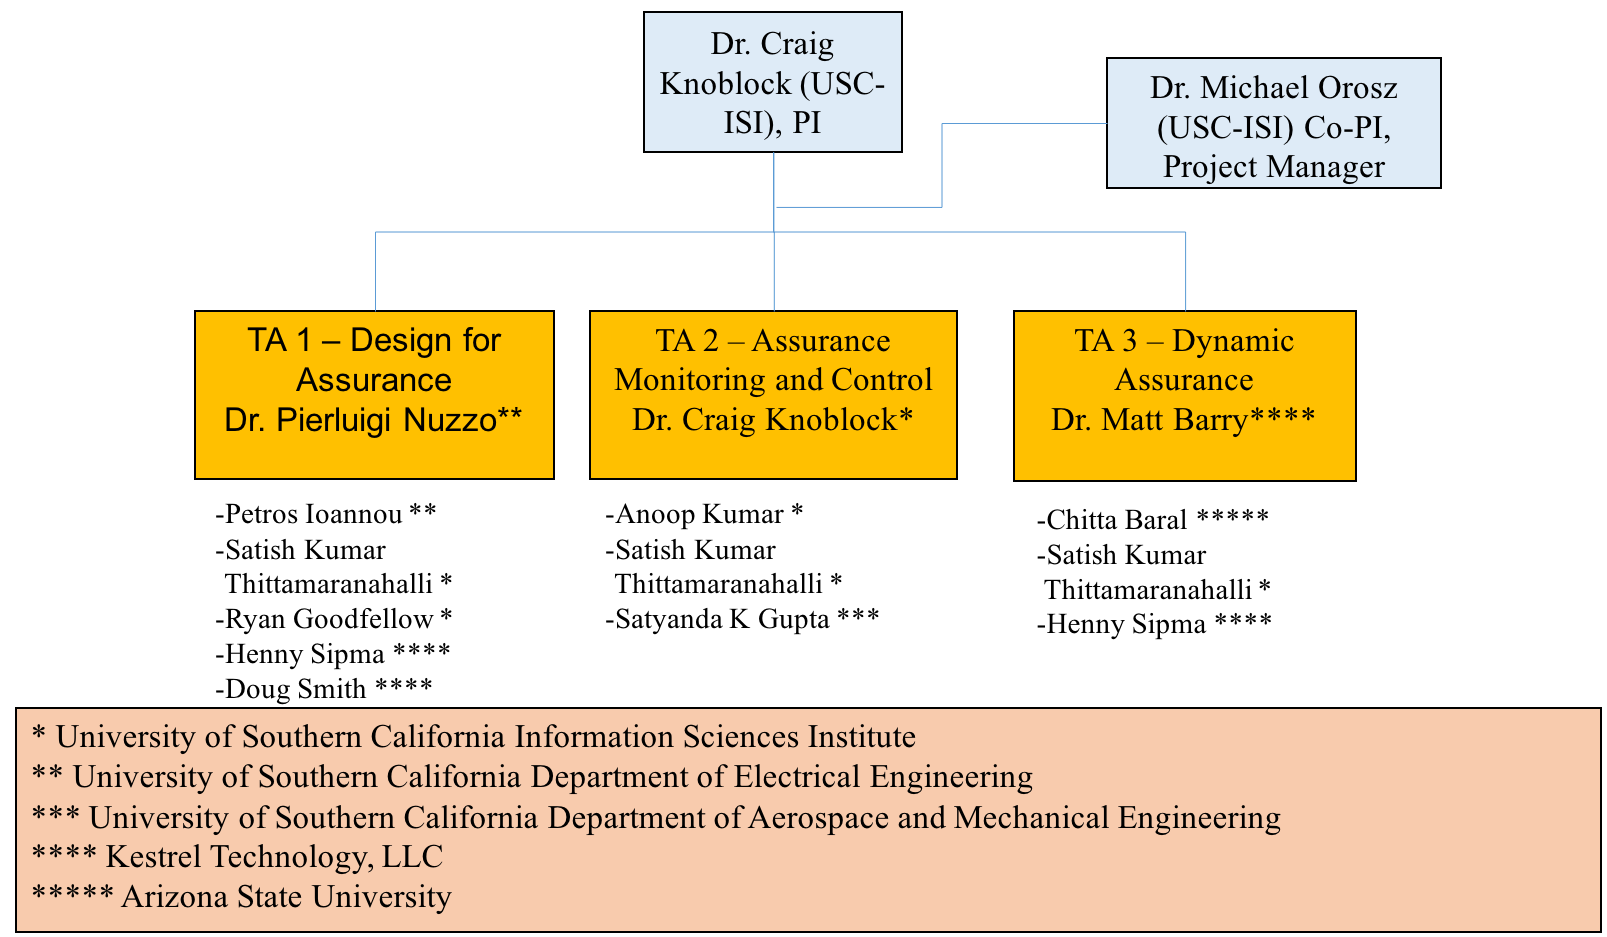
\includegraphics[width=6.0in]{./org-chart2.png}
\caption{\small Organization Chart}
\label{fig:org_chart}
\end{figure}

Coordination: To maximize collaboration and reduce risk to project failure from lack of communication and technical exchange, we plan to employ a wide variety of working styles and communication/coordination so that all can contribute.  At the core of our project will be regularly scheduled meetings bridging the diversely distributed team (Table~\ref{fig:Collaboration_Table}).  These meetings will address project status, identify challenges, implement risk mitigation strategies and participate in technology exchanges and system integration efforts (when appropriate)

\begin{table}[ht]
\caption{\small Project Meetings and Events}
  \centering
  {\footnotesize
\begin{tabular}{|m{3.15in}|m{3in}|} 
\hline
\textbf{Meeting} & \textbf{Frequency} 
\\\hline
Conference calls among investigators (discuss project status, address concerns and project risks) & Weekly
\\
\hline
Technical exchange and coordination meetings using Bluejeans or another videoconference technology & At least twice a month and more frequently as needed
  \\ 
\hline
Face-to-Face meetings (prior to P/I and demonstration meetings) & Every 3 to 6 months and more frequently (especially at the beginning of the project) as needed
 \\\cline{1-2}

\hline
\end{tabular}
}
\label{fig:Collaboration_Table}
\end{table}

\begin{table}[tbhp]
\caption{\small Key Project Team Member Responsibilities}
  \centering
  {\footnotesize
\begin{tabular}{| m{.75in} | m{3.9in}| m{1.5in}|} 
\hline
\textbf{Key Member} & \textbf{Responsibilities} & \textbf{Tasks} 
\\\hline
Dr.\ Craig Knoblock  & Principal Investigator responsible for project, leads TA 2 – Assurance Monitoring and Control.  Will lead the overall project and lead the TA2 team.  Served as the PI on many DARPA projects and has sucessfully led many large teams.    Effort on project:  25\% &
1.1.6, 1.2.2 1.2.3, 1.2.4, 1.3.4, 1.4.1, 
2.1.6, 2.2.2 2.2.3, 2.2.4, 2.3.4, 2.4.1, 
3.1.6, 3.2.2, 3.2.3, 3.2.4, 3.3.4, 3.4.1
\\
\hline
Dr.\ Michael Orosz & Co-Principal Investigator responsible managing the day-to-day operations of the project, assist technical teams as needed, coordinate with TA4 teams.    Has led many large complex multi-disciplined/multi-organizational projects in academic and industry environments.  Effort on project: 50\%
& 1.1.6, 2.1.6, 3.1.6, 1.4.1, 2.4.1, 3.4.1
  \\ 
\hline
Dr.\ Pierluigi Nuzzo 
& 
Co-Principal Investigator.  Leads the TA 1 - Design for Assurance team and conducts research on the formal methods for the design of the TA1 system.  Research experience on methodologies and tools for the design of cyber-physical systems; contracts, interfaces, and compositional methods for embedded system design; the application of automated formal methods and optimization theory to problems in embedded and cyber-physical systems.  Effort on project: 2 months/year (16.6\%)
& 
1.1.1, 2.1.1, 3.1.1 \\
\hline
Dr.\ Matthew Barry
& 
Key personnel.  Leads the TA 3 – Dynamic Assurance.   He will conduct the research on the dynamic assurance case language editors and parsers, the run-time system, and system integrations. Effort on project:  66\%
& 
1.3.2, 2.3.2, 3.3.2\\
\hline
Dr.\ Chitta Baral
& 
Key personnel responsible for learning assurance rules, supporting assurance rules with uncertainty and improving solver speed.  Expertise on ASP solvers, which will be used to reason about the assurance cases. Effort on project: 20\%
& 
1.3.1, 2.3.1, 3.3.1 \\
\hline
Dr.\ Doug Smith 
& 
Key personnel will support formal methods aspects of TA1, and lead the effort on abstract refinement. Expertise in field of automated correct-by-construction program generation.    Effort on project: 40\%
& 
1.1.5, 2.1.5, 3.1.5 \\
\hline
Dr.\ Henny Sipma
& 
Key personnel who will support the program verification tasks under TA1.  Will lead the effort on program verification.   Effort on project:  45\%
& 
1.1.5, 2.1.5, 3.1.5, 1.3.2, 2.3.2, 3.3.2 \\
\hline
Dr.\ Petros Ioannou
& 
Key personnel responsible providing and extending the assurance test bed, which will be available at the start of the project for autonomous vehicles.   Effort on project: 1 month/year (8.3\%)
& 
1.1.2, 2.1.2 (optional), 3.1.2 (optional)
\\
\hline
Dr.\ Satyandra Kumar Gupta
& 
Key Personnel providing autonomous command and control expertise to the TA-2 team.   Will lead the research on safety aware learning on TA2.   Past research on physics-aware decision making to facilitate automation.  Effort on project: 1 month/year (8.3\%)
& 
1.2.1, 2.2.1, 3.2.1 \\
\hline
Dr.\ Anoop Kumar 
& 
Key personnel providing support to the TA 2 project team.  Will lead the research on monitoring \& control and detecting distribution shifts.  Effort on project: 50\%
& 
1.2.1, 1.2.2, 1.2.3, 1.2.4, 2.2.1, 2.2.2, 2.2.3, 2.2.4, 3.2.1, 3.2.2, 3.2.3, 3.2.4\\
\hline
Dr.\ Satish Thittamaranahalli
& 
Key personnel developing scalable algorithms for TA1, TA2, and TA3 project teams.  Has extensive experience on scalable algorithm design, machine learning, and constraint reasoning.  Effort on project: 50\%
& 
1.2.1, 1.2.2, 1.2.3, 1.2.4, 2.2.1, 2.2.2, 2.2.3, 2.2.4, 3.2.1, 3.2.2, 3.2.3, 3.2.4, 1.1.4, 2.1.4, 3.1.4 \\
\hline
Dr.\ Ryan Goodfellow
& 
Key personnel providing support to the TA-1 project. Will lead the research on simulation-based testing.  Has extensive experience on simulation-based testing.  Effort on project:  30\%
& 
1.1.3, 2.1.3, 3.1.3 \\

\cline{1-2}

\hline
\end{tabular}
}
\label{fig:Table_Mgmt}
\end{table}



\newpage
\section{Personnel, Qualifications and Commitment}

{\bf Dr.\ Craig Knoblock}, the PI on this effort, is a Research Professor of both Computer Science and Spatial Sciences at the University of Southern California (USC) and Director of the Intelligent Systems Division at the USC Information Sciences Institute.   He received his Ph.D. from Carnegie Mellon University in computer science. 
%His research focuses on techniques for describing, acquiring, and exploiting the semantics of data.  
In previous projects he has worked on developing  scalable approaches to execution monitoring, accurate detection of sensor failures, and   automatic modeling and reconstruction of sensors.  He has published more than 300 journal articles, book chapters, and conference papers on these topics.  Dr. Knoblock is a Fellow of the Association for the Advancement of Artificial Intelligence (AAAI), a Distinguished Scientist of the Association of Computing Machinery (ACM), a Senior Member of IEEE, past President and Trustee of the International Joint Conference on Artificial Intelligence.
%and winner of the 2014 Robert S. Engelmore Award.  

{\bf Dr.\ Michael Orosz}, a Co-PI on this effort, is a Research Associate Professor of Civil and Environmental Engineering at the University of Southern California (USC) and Research Director of the Decision Systems Group at the USC Information Sciences Institute.  Dr. Orosz has over 30 years’ experience in commercial and government software development, basic and applied research, project management, academic research and has developed and deployed several commercially successful products.  His research interests are in machine learning and decision analytics as applied to intelligence analysis and autonomous command and control such as smart building controls.    Dr. Orosz has extensive experience in managing large complex multi-disciplined/multi-teamed research projects. %funded by DARPA, DHS, DoD, DoE, Industry, NASA, NRO, NSA and ONR.   
He received his Ph.D. in computer science from the University of California, Los Angeles.

{\bf Dr.\ Pierluigi Nuzzo}, a Co-PI on this project, is an Assistant Professor in the Department of Electrical Engineering at the University of Southern California. He received the Ph.D. in Electrical Engineering and Computer Sciences from the University of California at Berkeley. 
%in 2015, and the Laurea degree (MS) in electrical engineering (summa cum laude) from the University of Pisa, Italy, and the Sant'Anna School of Advanced Studies, Pisa, Italy.
%
%He has four years of research experience in analog and mixed signal circuit design as a researcher at IMEC, Leuven, Belgium, and over 10 years experience in design methodologies and tools for mixed-signal integrated circuits and cyber-physical systems, as a researcher at the University of Pisa, IMEC, UC Berkeley, and USC. 
His research interests
include: methodologies and tools for cyber-physical system and mixed-signal
system design; contracts, interfaces and compositional methods for embedded
system design; the application of formal methods and optimization theory to problems in embedded and cyber-physical systems and electronic design automation. 
%
Prof. Nuzzo received %First Place in the operational category and Best Overall
%Submission in the 2006 DAC/ISSCC Design Competition, 
a Marie Curie Fellowship
from the European Union in 2006, 
the University of California at Berkeley EECS
departmental fellowship in 2008, 
%the University of California at Berkeley Outstanding Graduate Student Instructor Award in 2013, 
the IBM Ph.D.
Fellowship in 2012 and 2014, 
%the Best Paper Award from the International Conference on Cyber-Physical Systems (ICCPS) in 2016, 
and the David J.~Sakrison Memorial Prize in 2016 for his doctoral research. 
%He is an author of 1 patent and over 60 publications.

{\bf Dr.\ Satyandra K. Gupta} is Smith International Professor in the Department of Aerospace and Mechanical Engineering at the University of Southern California. %Prior to joining the University of Southern California, he was a Professor in the Department of Mechanical Engineering and the Institute for Systems Research at the University of Maryland. He was the founding director of the Maryland Robotics Center and the Advanced Manufacturing Laboratory at the University of Maryland. 
He served as a program director for the National Robotics Initiative at the National Science Foundation from September 2012 to September 2014.  Dr. Gupta's interest is in the area of physics-aware decision making to facilitate automation. He has published more than 300 technical articles. He is a fellow of the American Society of Mechanical Engineers (ASME) and editor of ASME Journal of Computing and Information Science in Engineering. Dr. Gupta has received the Young Investigator Award from the Office of Naval Research in 2000, CAREER Award from the National Science Foundation in 2001, Presidential Early Career Award for Scientists and Engineers (PECASE) in 2001, Invention of the Year Award at the University of Maryland in 2007, Kos Ishii-Toshiba Award from ASME in 2011, and Excellence in Research Award from ASME in 2013.%, and Distinguished Alumnus Award from Indian Institute of Technology, Roorkee in 2014. %He has also received seven best paper awards at conferences.

{\bf Ryan Goodfellow} is a computer scientist at ISI working in combined cyber physical simulation and emulation platform development. His formal background is in simulation algorithms and modeling techniques using differential-algebraic equations (DAE). He has applied this knowledge in the CPS space by integrating DAE modeling languages and simulation engines with network testbeds to create comprehensive scientific experimentation platforms for cyber-physical systems. These experimentation platforms have been used in the power grid research space. %Ryan is a lead developer on the Deter network testbed, with a strong background in networked and distributed systems engineering. %He is also a combat veteran, serving as a non-commissioned officer and SIGINT team lead for a multi-functional intelligence team in Afghanistan.

{\bf Dr.\ Petros Ioannou} is a Professor in the Department of Electrical Engineering, Director of the Center for Advanced Transportation Technologies and Associate Director for Research for the DOT supported University Transportation Center at USC. He received his MS and PhD from the University of Illinois at Urbana Champaign in Mechanical and Electrical Engineering, respectively. His research interests are in robust adaptive control, vehicle dynamics and control, human factors and safety, automated vehicles, nonlinear systems and Intelligent transportation Systems.  He received the 2016 IEEE Transportation Technologies field award and the 2016 IEEE Control system society Transition to Practice Award. He is a Fellow of IEEE, IFAC and IET and author/coauthor of 8 books and over 400 papers.

{\bf Dr.\ Matthew Barry} will serve as lead for the TA3 tasks. %He will implement the dynamic assurance case language editors and parsers, the run-time system, and system integrations.  He will implement the assurance case arguments and the API for updating argument structure and content.  
Dr. Barry currently is CEO at Kestrel Technology LLC, and previously spent 20 years in NASA space mission operations at the Jet Propulsion Lab and Johnson Space Center.  At NASA Headquarters he led the introduction of dependability case requirements and plans for flight computing systems in upcoming manned space exploration missions, as well as the development of Agency-level software-related safety-critical control system requirements.  He recently served as a Principal Investigator on DHS/Cyber S\&T STAMP (Static Tool Analysis Modernization Program), DARPA CSFV (Crowd Sourced Formal Verification), three NASA Aeronautics R\&D projects, and the AFRL-sponsored Static Analysis of Numerical Algorithms project.  Dr. Barry earned BSME, MS, and PhD degrees in mechanical engineering, and an MBA degree, from Rice University.  

{\bf Dr.\ Henny Sipma} will support the program verification tasks under TA1.  %She is the key person behind the company's {\em KT Advance\/} and {\em KT Transferal\/} static analysis products, and the designer and programmer of the company's core {\em CodeHawk\/} abstract interpretation engine. 
Dr. Sipma currently is the CTO at Kestrel Technology LLC.  She has spent the past 10 years with Kestrel Technology as a static analysis expert; previously developed and taught static analysis techniques as senior research associate at Stanford University for eight years; and developed industrial process controls as an senior systems analyst at Shell.  She has been Principal Investigator or company lead on several recent R\&D projects for Federal agencies, including two projects under the IARPA STONESOUP (Securely Taking On New Executable Software of Uncertain Provenance) program; the DHS Cyber S\&T Gold Standard project; and the DARPA-sponsored STAC (Space-Time Analysis for Cybersecurity) and MUSE (Mining and Understanding Software Enclaves) programs.  Dr. Sipma earned 
%a BS degree in chemistry and an MS degree in chemical engineering at the University of Groningen in The Netherlands, and 
MS and PhD degrees in computer science from Stanford University.  

{\bf Dr.\ Douglas R.\ Smith} will support formal methods aspects of TA1, including the enforcement of safety properties and the generation of monitors.  He is President of Kestrel Technology LLC and Principal Scientist at Kestrel Institute.  He is a Fellow of the American Association of Artificial Intelligence (AAAI) and an ASE Fellow (Automated Software Engineering).  From 1986 to 2000, he taught an advanced graduate course on correct-by-construction software development at Stanford.  
%Dr. Smith has led the development of a series of software synthesis systems, including KIDS (Kestrel Interactive Development System), Specware, Designware, and Planware. 
%Applications domains have included a variety of complex high-performance planners and schedulers for the US Air Force.  He leads current projects on the generation of air mission plans and cyberoperations.  
Other recent projects focused on automated policy enforcement \cite{SmithD0703,SmithD08}, synthesis of secure network protocol codes, and the synthesis of high-performance constraint-solvers\cite{SmithD08c,SmithD13}.  Dr. Smith has over 30 years experience in the field of automated correct-by-construction program generation and has published over 100 papers. He has one patent.  He received the Ph.D. in Computer Science from Duke University% in 1979.  

{\bf Dr. Chitta Baral} is a Professor in the Department of Computer Science and Engineering at Arizona State University. He will support the TA3 efforts on Learning assurance rules, supporting assurance rules with uncertainty and improving solver speed. Dr. Baral has expertise in various aspects of autonomy and Artificial Intelligence. 
He wrote the first book on answer set programming (published by Cambridge University Press) the formal language behind our assurance rules. Some of his other works relevant to this proposal are: goal specification for autonomous systems, automatic construction of control rules for autonomous systems that satisfy given goals, combining machine learning with reasoning in various contexts, including image understanding. %He is the President of KR Inc. He is an associate editor of AIJ and has been an associate editor of JAIR.

{\bf Dr.\ Satish Kumar Thittamaranahalli (T. K. Satish Kumar)} leads the Collaboratory for Algorithmic Techniques and Artificial Intelligence (CATAI) at USC's Information Sciences Institute. He has published over 60 papers on numerous topics in Artificial Intelligence spanning such diverse areas as Constraint Reasoning, Planning and Scheduling, Probabilistic Reasoning, Robotics, Combinatorial Optimization, Approximation and Randomization, Heuristic Search, Model-Based Reasoning, Knowledge Representation and Spatio-Temporal Reasoning. %He %has served on the Program Committees of many international conferences in Artificial Intelligence
He and is a winner of the 2016 Best Robotics Paper Award and the 2005 Best Student Paper Award from the International Conference on Automated Planning and Scheduling. 
Dr. Kumar received his PhD in Computer Science from Stanford University. %In the past, he has also been a Visiting Student at the NASA Ames Research Center, a Postdoctoral Research Scholar at the University of California, Berkeley, a Research Scientist at the Institute for Human and Machine Cognition, a Visiting Assistant Professor at the University of West Florida, and a Senior Research and Development Scientist at Mission Critical Technologies.

\textbf{Dr.\ Anoop Kumar} is a senior computer scientist at USC ISI and has broad expertise in machine learning, statistical modeling, and software engineering.  Dr.\ Kumar is the technical lead on the DARPA RSPACE program and has played a vital role in developing a system that fuses air operations data from multiple sources, maintains world state, and issues warnings. Previously, he led the research and development of the BBN’s election forecasting system for the IARPA OSI program. %Dr.\ Kumar played a significant role in the DARPA DEFT program by developing a model to support integration of output from multiple NLP algorithms. He has contributed at the development to management levels on government research contracts and commercial projects. 
Dr.\ Kumar helped design and develop BBN's commercially available, hosted speech and medical transcription services offering. 

\begin{table}[!tbh]
\begin{footnotesize}
\vspace{-0.1in}

\begin{tabular}{lll}
\begin{tabular}[t]{|l|@{}c@{}|@{}c@{}|@{}c@{}|@{}c@{}|} \hline
Project & Status & \multicolumn{3}{ c| }{Hours} \\ \cline{3-5}
& & P1 & P2 & P3 \\ \hline



\multicolumn{5}{ |c| }{ \textbf{Craig Knoblock} } \\ \cline{1-5}
Safeguard & Pro & 770 & 641 & 641 \\ \cline{1-5}
ELICIT & Cur & 308 & 256 & 120 \\ \cline{1-5}
WTNIC & Cur & 11 & 0 & 0 \\ \cline{1-5}
EFFECT & Cur & 641 & 107 & 0 \\ \cline{1-5}
LinkedMaps & Cur & 203 & 25 & 0 \\ \cline{1-5}
PRINCESS & Cur & 608 & 96 & 0 \\ \cline{1-5}
SCHARP & Cur & 481 & 54 & 0 \\ \cline{1-5}
MINT & Pen & 650 & 534 & 285 \\ \cline{1-5}

\multicolumn{5}{ |c| }{ \textbf{Michael Orosz} } \\ \cline{1-5}
Safeguard & Pro & 1560 & 1300 & 1300  \\ \cline{1-5}
SMC/SY & Cur & 1803 & 0 & 0  \\ \cline{1-5}

\multicolumn{5}{ |c| }{ \textbf{Matthew Barry} } \\ \cline{1-5}
Safeguard & Pro & 2078 & 1690 & 1554 \\ \cline{1-5}
Starlite & Cur & 1840 & 1692 & 0 \\ \cline{1-5}



\multicolumn{5}{ |c| }{ \textbf{Anoop Kumar} } \\ \cline{1-5}
Safeguard & Pro & 1560 & 1300 & 1300 \\ \cline{1-5}

\end{tabular}
&
\begin{tabular}[t]{|l|@{}c@{}|@{}c@{}|@{}c@{}|@{}c@{}|} \hline
Project & Status & \multicolumn{3}{ c| }{Hours} \\ \cline{3-5}
& & P1 & P2 & P3 \\ \hline

\multicolumn{5}{ |c| }{ \textbf{Pierluigi Nuzzo} } \\ \cline{1-5}
Safeguard & Pro & 520 & 433 & 433  \\ \cline{1-5}
Mirage & Cur & 433 & 0 & 0  \\ \cline{1-5}

\multicolumn{5}{ |c| }{ \textbf{Satyandra Gupta} } \\ \cline{1-5}
Safeguard & Pro & 260 & 217 & 217 \\ \cline{1-5}
Human   & Cur & 22 & 0 & 0 \\ \cline{1-5}
Vehicles & Cur & 36 & 0 & 0 \\ \cline{1-5}
Robot & Cur & 116 & 0 & 0 \\ \cline{1-5}
Assembly & Cur & 33 & 0 & 0 \\ \cline{1-5}
Solar & Cur & 4 & 0 & 0 \\ \cline{1-5}

\multicolumn{5}{ |c| }{ \textbf{Petros Ioannou} } \\ \cline{1-5}
Safeguard & Pro & 260 & 217 & 217 \\ \cline{1-5}
CPS & Cur & 130 & 0 & 0 \\ \cline{1-5}

\multicolumn{5}{ |c| }{ \textbf{Ryan Goodfellow} } \\ \cline{1-5}
Safeguard & Pro & 936 & 780 & 780 \\ \cline{1-5}
STEAM & Cur & 416 & 0 & 0 \\ \cline{1-5}


\end{tabular}
&
\begin{tabular}[t]{|l|@{}c@{}|@{}c@{}|@{}c@{}|@{}c@{}|} \hline
Project & Status & \multicolumn{3}{ c| }{Hours} \\ \cline{3-5}
& & P1 & P2 & P3 \\ \hline

\multicolumn{5}{ |c| }{ \textbf{Chitta Baral} } \\ \cline{1-5}
Safeguard & Pro & 659 & 485 & 485 \\ \cline{1-5}
PostdocBP & Cur & 176 & 0 & 0 \\ \cline{1-5}
Languages & Pen & 528 & 264 & 264 \\ \cline{1-5}
CAREER & Pen & 88 & 44 & 44 \\ \cline{1-5}
CHS & Pen & 510 & 255 & 0 \\ \cline{1-5}

\multicolumn{5}{ |c| }{ \textbf{Doug Smith} } \\ \cline{1-5}
Safeguard & Pro & 1222 & 984 & 840 \\ \cline{1-5}
RSPACE & Cur & 342 & 0 & 0 \\ 
\cline{1-5}
PLANX & Cur & 154 & 0 & 0 \\ 
\cline{1-5}
HACCS & Pen & 923 & 769 & 769 \\ 
\cline{1-5}

\multicolumn{5}{ |c| }{ \textbf{Henny Sipma} } \\ \cline{1-5}
Safeguard & Pro & 1372 & 962 & 840 \\ \cline{1-5}
STAC & Cur & 797 & 0 & 0 \\ \cline{1-5}

\multicolumn{5}{ |c| }{ \textbf{Satish Thittamaranahalli} } \\ \cline{1-5}
Safeguard & Pro & 1560 & 1300 & 1300 \\ \cline{1-5}
MapF & Cur & 103 & 103 & 0 \\ \cline{1-5}

\end{tabular}
\end{tabular}

\end{footnotesize}
\caption{Individual commitments of key personnel}
\label{tab:Commitments}
\vspace{-0.2in}
\end{table}

\clearpage
\newpage
\section{Capabilities}


%\subsection{University of Southern California}
USC has strengths in number of areas that are closely related to the proposed work:
\begin{itemize}[itemsep=0pt,leftmargin=*]
\item Dr.\ Nuzzo 
%has over 10-year research experience in embedded system design, from mixed-signal chip design (analog-to-digital converters, frequency synthesizers, software-defined radio), to methodologies and tools for mixed-signal integrated circuits and Cyber-Physical Systems (CPSs), and the application of formal methods and optimization theory to problems in embedded and cyber-physical systems and electronic design automation.  
%His doctoral work 
has done extensive research on contracts and compositional methods for heterogeneous system design and design space exploration, with application to aircraft electric power systems and environmental control systems. His work has helped transition rigorous system design foundations, innovative design methodologies, and new systems engineering paradigms to industry (IBM, United Technologies). 
\item Dr.\ Satyandra K. Gupta has worked on autonomous surface vehicles, autonomous ground vehicles for operation on rugged terrains, and autonomous flapping wing aerial vehicles.   His group has developed a hierarchal decision making approach for realizing autonomous systems. 
%This approach combines task planning and assignment, deliberative trajectory planning, reactive collision avoidance behaviors, and trajectory tracking control layers. 
His group has also developed new methods for learning reactive behaviors in adversarial environments and COLREGS compliant trajectory planning. \item Dr.\ Knoblock has developed methods that learn the relationships between sensors to both identify failures and changes in sensor and reconstruct those sensors, providing estimates of the accuracy of the reconstructed sensors.  
\item Ryan Goodfellow has extensive experience in simulation based testing through high-fidelity CPS testbed environment development and operation, using the Deter network testbed as the core which has supported several large scale government projects from a variety of agencies and thousands of users. %we have developed sophisticated CPS experiments under programs such as NFS RIPS, NIST SmartCities and the DHS Cybersecurity showcase.
\item Dr.\ Ioannou %helped  design and implement adaptive cruise control systems in collaboration with Ford Motor Company, which was commercialized four years before any other company. He 
worked on several DOT funded projects on automated vehicles and intelligent highway systems where he demonstrated his vehicle control designs for safety and performance on actual automated vehicles in test trucks and I-15 highway.
\item Drs.\ Knoblock, Kumar, and Thittamaranahalli have developed highly scalable approaches for monitoring message traffic to identify potential problems and issue warnings and alerts. 
\item Dr. Thittamaranahalli has developed state-of-the-art methods for efficiently solving large-scale search and optimization problems. %These techniques will be applicable in TA2 for safety-aware learning and planning, in TA2 for assurance monitoring and control, and in TA3 for dynamic assessment of assurance cases.

\end{itemize}
%\subsection{Kestrel Technology LLC}

Kestrel Technology's strength is in program analysis, specifically static analysis of both source and binary targets.  The company performs applied R\&D and product development for a variety of static analysis applications  pivoting primarily on the abstract interpretation technique.  The company recently initiated development of program analysis applications using logical equivalence techniques. As a provider of verification evidence in the form of mathematical proofs, the company also has expertise in the design and development of assurance case arguments for high-integrity systems using such evidence. %The company is engaged in a partnership with Wind River Systems to develop program analysis tools for its embedded system developers.  Many of Wind River's customers must develop their products under safety and certification standards, including those using safety cases.  

   

%\subsection{Arizona State University}
Chitta Baral at Arizona State University has developed various software to learn assurance rules and various ASP solvers, which he has made available as open-source.

Most of the software carried forward for implementation or derivation is open source.  The single exception is Kestrel Technology's {\it KT Advance\/} static analysis tool (TA1), in particular the abstract interpretation engine therein, which is company proprietary and is US EAR export-controlled.   
%Owing to mixed funding for the development of that technology 
We will continue to provide the Federal government a restricted use license for that particular item.

There are no specialized facilities, data, or GFE required for this effort. 

\include{sow}
\include{milestones}

% \section{Level of Effort by Task \textcolor{red}{[Mike/Lisa - 1 pages]}}

% \textcolor{blue}{
% \begin{itemize}
% \item Will be a separate spreadsheet
% \item
% \end{itemize}
% }

\include{appendix_a}

%\section{Appendix B \textcolor{red}{[No Page Count]}}

\section{References}
\bibliographystyle{acm} 
\bibliography{TA3/ta3,TA2/ta2,TA1/ta1}
\end{document}
%%\documentclass[a4paper]{article}
%\documentclass[12pt]{article}
\documentclass[12pt]{dod-blank}

%% Language and font encodings
\usepackage[english]{babel}
\usepackage[utf8x]{inputenc}
\usepackage[T1]{fontenc}

%% Sets page size and margins
%%\usepackage[a4paper,top=3cm,bottom=2cm,left=3cm,right=3cm,marginparwidth=1.75cm]{geometry}
%\usepackage[top=1in, bottom=1in, left=1in, right=1in]{geometry}



%% Useful packages
\usepackage{amsmath}
\usepackage{graphicx}
  \graphicspath{{.}{./image/}}
  \DeclareGraphicsExtensions{.png,.jpg} 
\usepackage[colorinlistoftodos]{todonotes}
\usepackage[colorlinks=true, allcolors=blue]{hyperref}
\usepackage{tabularx}
\usepackage{multirow}
\usepackage{tabulary}
\usepackage{float}
\usepackage{wrapfig}
\usepackage[export]{adjustbox}
\usepackage{comment}
\usepackage{tabularx}
\usepackage{multirow}
\usepackage{tabulary}
\usepackage{enumitem}

\usepackage{listings}
\usepackage{color}
\usepackage{array}
\usepackage{subcaption}
\usepackage{xcolor}




\renewcommand{\textfraction}{0}
\renewcommand{\topfraction}{1.0}
\renewcommand{\bottomfraction}{1.0}

\usepackage{longtable}
%% macros
\newif\iffinal
\finaltrue
\iffinal
  
    \newcommand\baareq[1]{}
    \newcommand\baades[1]{}
 
 
\else
    \definecolor{darkgreen}{rgb}{0,0.4,0}
    \definecolor{darkcyan}{rgb}{0,0.4,0.4}
    \definecolor{darkblue}{rgb}{0,0,0.5}
    
    \newcommand\baareq[1]{{\color{darkcyan}[\textbf{Requirement:} #1]}}
    \newcommand\baades[1]{{\color{darkcyan}[\textbf{Description:} #1]}}
 
\fi




\def\naive{na\"{\i}ve}



\lstset{ 
  backgroundcolor=\color{white},   % choose the background color; you must add \usepackage{color} or \usepackage{xcolor}
  basicstyle=\footnotesize\ttfamily,            % the size of the fonts that are used for the code
  breakatwhitespace=false,         % sets if automatic breaks should only happen at whitespace
  breaklines=true,                 % sets automatic line breaking
  captionpos=b,                    % sets the caption-position to bottom
  commentstyle=\color{mygreen},    % comment style
  % deletekeywords={...},            % if you want to delete keywords from the given language
  escapeinside={\%*}{*)},          % if you want to add LaTeX within your code
  extendedchars=true,              % lets you use non-ASCII characters; for 8-bits encodings only, does not work with UTF-8
  frame=single,	                   % adds a frame around the code
  keepspaces=false,                 % keeps spaces in text, useful for keeping indentation of code (possibly needs columns=flexible)
  keywordstyle=\color{blue}\bfseries\underbar,       % keyword style
  language=Prolog,                 % the language of the code
  % morekeywords={if,and},        % if you want to add more keywords to the set
  numbers=none,                    % where to put the line-numbers; possible values are (none, left, right)
  numbersep=5pt,                   % how far the line-numbers are from the code
  numberstyle=\tiny\color{mygray}, % the style that is used for the line-numbers
  rulecolor=\color{black},         % if not set, the frame-color may be changed on line-breaks within not-black text
  showspaces=false,                % show spaces everywhere adding particular underscores; it overrides 'showstringspaces'
  showstringspaces=false,          % underline spaces within strings only
  showtabs=false,                  % show tabs within strings adding particular underscores
  stepnumber=2,                    % the step between two line-numbers. If it's 1, each line will be numbered
  stringstyle=\color{mymauve},     % string literal style
  tabsize=2,	                   % sets default tabsize to 2 spaces
  title=\lstname                   % show the filename of files included with \lstinputlisting; also try caption instead of title
}

% apply trick for additional keywords for our AC DSL
\lstset{
	emph={for, if, and, or},
    emphstyle={\color{blue}\bfseries\underbar}
}




\title{DARPA Assured Autonomy}
\author{Technical Volume- \textcolor{red}{Thirty-Eight (38) pages max}}

\begin{document}
\pagenumbering{roman}
\include{cover}

\newpage
\section{Table of Contents}
\tableofcontents

\newpage
\pagenumbering{arabic}
\section{Executive Summary}
As we rapidly move into a world where machine learning plays a central role in realizing autonomous systems, it is becoming increasingly important to develop techniques that assure that these systems will operate safely and perform as expected. Current approaches are limited to providing assurance for systems with limited or no  learning capabilities. In this context, DARPA's Assured Autonomy BAA seeks to \emph{develop rigorous design and analysis technologies for continual assurance of learning-enabled autonomous systems}. USC in collaboration with Kestrel Technology and ASU is pleased to submit a comprehensive TA1, TA2, and TA3 proposal entitled \emph{``Assured Autonomy for Learning Enabled Vehicles (Safeguard).''} We plan to provide an end-to-end solution to support autonomous systems with learning-enabled components, ranging from design technologies for assurance, to assurance monitoring and control techniques, to representation and online evaluation of assurance cases. We have assembled a strong team of experts that cover the range of technologies that are required to create such an end-to-end system. If successful, the project will provide the technologies for building the next-generation of learning-enabled autonomous systems.  The entire project will take four years and cost \textcolor{red}{\$??}, with an initial version completed at the end of Phase I and successive versions with additional capabilities and improved scalability at the end of Phase II and Phase III.  

In the remainder of this section, we first introduce an  unmanned surface vehicle scenario that will be used throughout the proposal to describe the approach.  Next, we describe our approach to design, monitoring, and dynamic assurance. Finally, we introduce the team involved in the project. 

\textbf{Motivating Scenario.} Consider an autonomous unmanned surface vehicle (USV) guarding a valuable asset in the ocean when an unknown vehicle  approaches the security perimeter, under challenging weather conditions. In this scenario, the USV is required to approach the intruding vehicle, issue a warning signal, and escort it to a safe distance from the controlled area. However, as the USV has no a priori knowledge of its external environment behaviors (e.g., water depth, waves, wind, current, visibility), pre-computing a feasible trajectory, let alone optimal, becomes a non-trivial problem. For trajectory planning, the USV must continuously perform the following tasks:
\begin{itemize}[itemsep=0pt,leftmargin=*]
 \item Sense the current state of the surrounding environment (e.g., water depth, waves, wind, current, visibility) and estimate its own maneuverability constraints (e.g., braking distance, available acceleration, maximum velocity, turning radius, turning rate, safety distance) based on the state of the environment;      
\item Sense the static obstacles in the sensor range and generate a traversability map;
\item Sense the moving obstacles and classify them;   
\item Predict future trajectories of moving obstacles; 
\item Determine if any of the COLREGS \cite{commandant1999international} rules will be in effect with respect to one or more of the nearby vessels and identify the vessels with the right of way.    
\end{itemize}
The above information will be used by the trajectory planner to compute an initial trajectory, which will be continuously refined as the USV gathers additional information.
% It is not possible for the USV to be tested in every possible environment. 
The USV will use learning enabled components to take  decisions as it encounters new situations, such as  
\begin{itemize}[itemsep=0pt,leftmargin=*]
\item Classifiers to identify moving obstacles based on physical appearance and motion signatures,
\item Algorithms to estimate the sensor capabilities in adverse weather conditions,   
\item Algorithms to accurately estimate uncertainty in the environment, 
\item Classifiers to generate traversability maps,
\item Prediction of external vessel behaviors based on motion histories, 
\item Reinforcement learning  to ensure COLREGS compliance of maneuvers,  
\item Algorithms to learning pursuit behaviors.  
\end{itemize}
Learning enabled components will interact with each other in complex ways, where a misclassification error in one component may eventually compromise the entire mission.   
% We will need to make sure that each learning enabled components has a run-time monitor that will ensure that the assumptions made by the learning-enabled component remain valid and prevent erroneous learning. 
% For example, if the vehicle is exhibiting significant error in trajectory tracking, then simply downgrading the trajectory tracking error value may not be a good option.  The failure of prediction of trajectory tracking error might be due to the presence of a significant wake caused by a nearby vessel. The presence of the nearby vessel can be used to explain the degradation in trajectory tracking performance. As the vessel moves away, we can expect the trajectory tracking performance to return to the predicted level.  
While exhaustive validation of learning-enabled cyber-physical systems (LE-CPSs) is a prohibitive task~\cite{Kalra16},
their complexity, heterogeneity, and highly dynamic nature
make it challenging to even leverage existing model-based development techniques to effectively assess system correctness 
% dependability, 
at design time or enforce it at runtime.

\textbf{Design for Assurance.} Safeguard uses a platform-based design approach~\cite{Nuzzo15b} to organize the design process for a LE-CPS and to build assurance cases. Composite models are developed at several levels of abstraction,
from top-level system requirements and safety constraints down to the
implementation level.  Intermediate levels add detail to the levels
above.  The different levels are connected by refinement mappings that
allow properties established at one level to be preserved at the next
level (see Figures~\ref{fig:methodology} and~\ref{fig:assurance}).

Contracts are used to formally specify components and composite models
in terms of (1) Assumptions -- the assumed behaviors of the
environment and the behaviors of other components, and (2) Guarantees
-- the behavior properties that a model guarantees if it operates in a
context that satisfies its assumptions.  A calculus of contracts
allows horizontal composition of contracts to generate contracts for
composite models.  Vertical contracts are used to specify the mapping
or refinement relation between models at different levels of
abstraction.  The system design process starts with a high-level
contract that expresses overall system assumptions and requirements.
Subsequent levels express models with increasing detail until the
lowest level expresses the system in terms of hardware components and
their software controllers.

The assurance case for a CPS arises from the horizontal and vertical
structure of the design in several ways.  The components used within a
particular level are either (1) synthesized using
correct-by-construction design tools together with proofs, (2) derived
statically or dynamically using safety-aware machine-learning
techniques, (3) written manually and verified by analysis tools, or
(4) written manually and validated by extensive testing.  The
assurance case for the whole reflects its compositional structure.  We
anticipate that well-specified contracts together with the calculus of
contracts will eliminate well-known problems with unexpected emergent
behaviors in CPS systems.

The assurance case for the lowest-layer design arises from both the
intra-level assurance and from properties and their proofs that are
preserved under the refinement mapping from the top-level
requirements.  The refinement mappings between model layers will be
constructed using a variety of techniques.  A contract at an abstract
level can be mapped to a component or refined contract by (1)
retrieval of pre-verified components from a platform library, (2)
synthesis using correct-by-construction design and optimization tools,
or (3) manual coding to satisfy a contract.  The mapping of a
composite model will be composed from the mappings of its constituent
components or contracts.  When a composite model cannot be mapped
compositionally to the next level, it will be generated using
correct-by-construction design and optimization tools.

\textbf{Assurance Monitoring and Control.}
We provide an integrated framework for safety-aware learning, assurance monitoring and control, detecting distribution shifts. Three major components offer an efficient TA2 architecture as well as interfaces with TA1 and TA3, that is, (a) safety-aware learning and planning, (b) assurance monitors for guarding architectural and safety constraints; and (c) distribution shift detection.

We will develop a new learning-enabled online decision-making framework that allows opportunistically composing a sequence of actions (maneuvers) to reduce uncertainty in the system capability model without suspending the progress toward the mission goals or compromising safety. Each candidate action is evaluated based on three criteria: (1) the risk of violating a safety constraint using the current uncertainties in the parameter estimates; (2) its relevance to the mission goals; (3)  its expected information gain, i.e., reduction in uncertainty, with respect to the parameter estimates. These evaluations are combined to produce a cumulative mission utility value for each action that drives our learning-enabled decision-making framework. The problem of generating and evaluating sequences of actions can be posed in several way. For example, it can be solved using a branch-and-bound search method like Anytime A*, or formulated with the finite-horizon Markov Decision Process (MDP) framework. We will develop new scalable search strategies to solve this problem efficiently, by potentially evaluating a recent method developed at USC, called FastMap, that can significantly improve the execution time. 

We will develop monitors for architectural and safety constraints. 
% While these constraints can be checked over and over again as sensor information flow in, this naive strategy accounts for a lot of computational overhead. 
To achieve scalability and decrease the overhead, we propose the application of a technique that we currently use in DARPA's RSPACE program, which leverages a physical model of the vehicles dynamics and its interactions with the environment to efficiently determine the readout frequency. We propose two  extensions of this basic idea. First, we will use the theory of Variable Elimination to prioritize which variables to monitor, e.g., controllable, versus uncontrollable, adversarially controlled, or unobservable variables. Second, we invoke the dynamic assessment of assurance cases only when needed. This  decreases the number of times dynamic assessment of assurance cases is initiated as well as the communication bandwidth between the TA2 and TA3 components.

Finally, we will identify a distribution shift by combining statistical and machine learning techniques to differentiate between environmental and sensor changes. We will exploit a categorization of the shifts based on their cause and duration as well as extend our earlier work on detecting and mitigating sensor failures for all types of monitored variables.  

\textbf{Dynamic Assurance:} The Safeguard {\em design for assurance\/} activity takes a systems-theoretic stance toward safety.  Consequently, it presumes that safety is an emergent property of the system, and that hazards can present themselves through unintended interactions and performance violations in addition to causal events such as component failures.  Our design approach includes consideration of intent as well as hazard analysis and mitigation.  The artifacts from these activities populate contracts and assumptions for the dynamic assurance case.  
We thus build safety into the product by working at a systems-level viewpoint, using lexicon and design patterns familiar to both hardware and software engineers; safety is an emergent property of the system, not an afterthought.  
As system behavior evolves during runtime owing to learning, threats, degradation, or some other factor, the dynamic assurance case identifies whether the safety constraints continue to be satisfied.  If not, it provides notifications or issues recovery instructions directly from a lookup table.

Our implementation of the dynamic assurance case employs a declarative knowledge base inference engine and a domain-specific language tailored to our approach.  We have used them successfully for assurance case tool sets and arguments, and will extend them to reason about uncertainty and learning.  Our approach to achieve scalability is to specialize solvers toward modularity and to take advantage of domain knowledge.  Specifically, we will develop answer set programming techniques for context-dependent learning for reasoning about the learning-enabled components as well as learning assurance rules.  We will develop new formalisms for uncertainty to include causality, using weights for computing probabilities, and probabilistic non-monotonicity.  To achieve scaling objectives we will implement specializations using modularity, weighted CSPs, and message passing. 

% The system safety constraints revealed from that design become the key elements of our dynamic assurance case.  Our verification tools ensure the constraints are relevant, identifiable, and their implementation and effect observable.  

\textbf{Team.} We have assembled a team that is exceptionally well-qualified to build the proposed Safeguard system.  The team will be led by Dr.\ Craig Knoblock, the Principal Investigator for the effort, who currently leads the Intelligent Systems Division at the Information Sciences Institute.  He has led many large DARPA and IARPA projects over the years and has a strong track record in conducting leading edge research and then transitioning the technology to commercial use.  He will be supported by Dr.\ Michael Orosz as the Project Manager, who also has  experience in managing large research projects and on autonomous systems.  The TA1 team will be led by Dr.\ Pierluigi Nuzzo, who is an expert in embedded system design methodologies and the  application of formal methods to cyber-physical systems.  The TA1 team also includes Dr.\ Doug Smith, who has spent many years working on scalable correct-by-construction techniques and Dr.\ Henny Sipma, who has significant experience in applying program verification methods to real-world problems.  The TA1 team also includes Ryan Goodfellow, who has done a large amount of work on simulation-based testing.  The TA2 team will be led by Dr.\ Knoblock who has worked on topics related to both monitoring and detecting distribution changes.  He will be supported by Dr.\ Satyandra Gupta, who is an expert on autonomous surface vehicles as well as on safety-aware learning. He will also be supported by Drs.\ Anoop Kumar and Satish Thittamaranahalli, who have also previously worked on efficient methods for execution monitoring.  The TA3 team will be lead by Dr.\ Matthew Barry, who has experience in creating the technologies for assurance cases.  He will be supported by Dr.\ Chitta Baral, who is an expert on ASP solvers and by Dr.\ Thittamaranahalli who is an expert on SAT solvers, both of which will be applied to provide scalable assurance case reasoning.  Finally, Dr.\ Petros Ioannou, who is an expert on control systems for autonomous vehicles will provide an autonomous vehicle platform, which will form the focus of our work until the TA4 teams provide additional vehicle platforms for development.  

\newpage
\section{Innovative Claims and Deliverables}

In this project we will develop and build an end-to-end system for assured autonomy.  This section describes the key innovations by technical area and then the overall deliverables of the project.

\paragraph{Design for Assurance}

\begin{itemize}[itemsep=0pt,leftmargin=*]
\item We address the LE-CPS design challenges via a holistic approach that can contextually generate design artifacts and assurance cases. We develop a compositional, contract-based modeling framework, methods, and tools to support the design process from system-level requirement capture,  formalization, and analysis, to the generation, testing, and continual monitoring of software and hardware artifacts in feedback loop with a physical process.

\item We develop compositional abstractions and interfaces (vertical contracts) that can  bridge heterogeneous formalisms and heterogeneous decomposition architectures to make system analysis and synthesis tractable, consistently combine different verification and synthesis methods at design time, and provide seamless support for dynamic assurance at run time. %We aim to quantitatively capture the confidence in the satisfaction of requirements under uncertain or unknown conditions, and resilience properties of  systems at different abstraction levels, to enable trade-off evaluation between resilience, performance, and cost.

\item We develop a unifying framework and efficient algorithms to reason about the combination of discrete and continuous dynamics and constraints in the presence of uncertainties in LE-CPS using a satisfiability modulo convex approach~\cite{Shoukry2017} for contract-based system verification and scalable trajectory planning.  

\item We provide an environment for high-fidelity CPS testing, in which production-ready software, e.g.,  safety-critical learning and control, may be deployed and tested 
% by extending the Cypress testbed environment \cite{Goodfellow2015Cypress:Systems} 
with time dilation facilities, so that it synchronizes with a physical simulation that is not necessarily running in real time, while still having the perception of real time.

\item We 
% These facilities allow a cyber system to be  
propose an approach for unanticipated behavior space identification and test coverage maximization which leverages results from the theory of differential algebraic equation (DAE)~\cite{Berger2013ControllabilitySurvey,Ilchmann2005ATheory,BergerOnSystems,Lamour2013} 
to prune the behavior search space and identify smaller regions of interest for efficient simulation-based testing. 
% We then compute the intersection of these two behavior spaces and restrict our simulation based testing search space to this subspace.
\end{itemize}

\paragraph{Assurance Monitoring and Control}

\begin{itemize}[itemsep=0pt,leftmargin=*]
\item 
%We integrate safety-aware learning into the overall decision making problem. The goal is to maximize mission utility without violating the safety constraints. 
Our safety-aware learning framework enables the system to opportunistically select and execute actions to assist the learning-enabled component in reducing model uncertainty without compromising safety or deviating from the mission goals. The value of uncertainty reduction is explicitly incorporated in the optimization process for selecting the best action.  
\item For safety-aware learning, we propose the idea of preprocessing the search space of the problem domain before queries and observations come in. With such a linear-time preprocessing phase, the performance of search and optimization algorithms can be significantly boosted. For example, in regular A* search, the intensional or extensional search space can be preprocessed in near-linear time to yield an embedding of each state as a point in Euclidean space~\cite{cujakk}. Then, when the query comes in, A* search can make use of these Euclidean distances as heuristic distances between two states to yield order-of-magnitude speedups. 
%In Anytime A* for safety-aware learning and planning, this leads to a significantly better quality of actions chosen within a time limit, and in the MDP framework, the same ideas can be used to improve the convergence of Bellman updates for safety-aware Reinforcement Learning.
\item As massive amounts of sensor information flow in, it is imperative for us to efficiently process this information for monitoring architectural and safety constraints. Building on our past work on similar tasks, we propose novel technologies for efficiently monitoring constraints. These algorithms can yield an exponential reduction in the amount of sensor data that needs to be processed. Doing this also reduces the message complexities between the various modules. %We also propose to use the theory of Variable Elimination (VE) to monitor constraints with uncontrollable, adversarially controlled, and/or unobservable variables. VE yields a substrate constraint to monitor that characterizes a dominant strategy of the controllable variables over the uncontrollable, adversarially controlled, and/or unobservable variables.
\item We will develop techniques to identify  distributional shifts and determine the underlying cause (e.g., change in environment, sensor failure,   etc.), as well as strategies for handling the various distributional shifts.   Notably, we propose to build on our past work and use compact representations to exploit historical data to identify distributional shifts.
\end{itemize}

\paragraph{Dynamic Assurance}

\begin{itemize}[itemsep=0pt,leftmargin=*]

\item We demonstrate the integration of dynamic assurance for safety-critical learning-enabled dynamic systems in which evolutionary behaviors are expected and tolerated as a property of the functionality.   The impact will be consequential contributions safety-critical dynamic systems in which evolutionary behaviors are expected and tolerated as portion of the functionality.   
\item We implement dynamic assurance by combining features of system safety, formal methods, logic programming, uncertain reasoning, and domain-specific languages.  We populate assurance case arguments at several levels of modeling and implementation abstraction, using the analysis results to produce design-time evidence supporting assurance claims.  
%We provide automated reasoning about the assurance case itself to produce verification, consistency, and completeness results for the argument.  Dynamic assurance results then yield trusted explanations of whether safety constraints and assumptions and other contracts still hold during the collection of runtime evidence from monitors. 
\item We develop and demonstrate ASP formalisms crucial to applications in dynamic assurance. We demonstrate the suitability of the technology especially for assurance case arguments owing to the improved legibility, consistency and completeness checks, handling of uncertain and default reasoning, and scalability.  
%We will produce modularized solvers for enhanced performance based on recent algorithmic developments in exploiting structure, kernelization, and message passing. We provide a formalism to enable learning of assurance rules. 
We provide a novel approach to handling uncertainty that provides the ability to do causal and counter-factual reasoning as well as probabilistic non-monotonicity.  Overcoming limitations of traditional inductive logic techniques, we develop a novel iterative and incremental approach based on context dependent learning. 
\end{itemize}

\paragraph{Deliverables}
During the course of this project, we will build and deliver a fully-operational system that covers all three of the technical areas.  The detailed capabilities of this system are described in the individual technical sections.  The resulting system will be available as open source under a permissive license, which will allow other organizations to use the work, extend it in new directions, and even commercialize the software.  Kestrel Technology has significant experience in this space and has built and applied these types of technologies to a variety of real world tasks.  Kestrel is ideally suited to pursue commercial uses of this technology and the permissive license will facilitate exploring these opportunities since there will be no need to negotiate intellectual property rights.  

\newpage
\section{Technical Plan}
\input{./TA1/main}
\input{./TA2/main}
\input{./TA3/main}
\clearpage
\newpage


\section{Management Plan}


The Principal Investigator for this effort is Dr. Craig Knoblock who is responsible for all aspects of the effort, will coordinate the parallel team efforts, and will ensure high levels of performance from individual team members.  The Co-P/I, Dr. Michael Orosz, will provide project management and will assist all performers in the execution of the project.    The project team is divided into three working groups (Figure~\ref{fig:org_chart}) corresponding to Technical Areas 1-3, however, members of each team contribute across all project activities.   Table~\ref{fig:Table_Mgmt} defines the major contributions of each project team member to the project tasks.

\begin{figure}[tbhp]
%\vspace{-25pt}
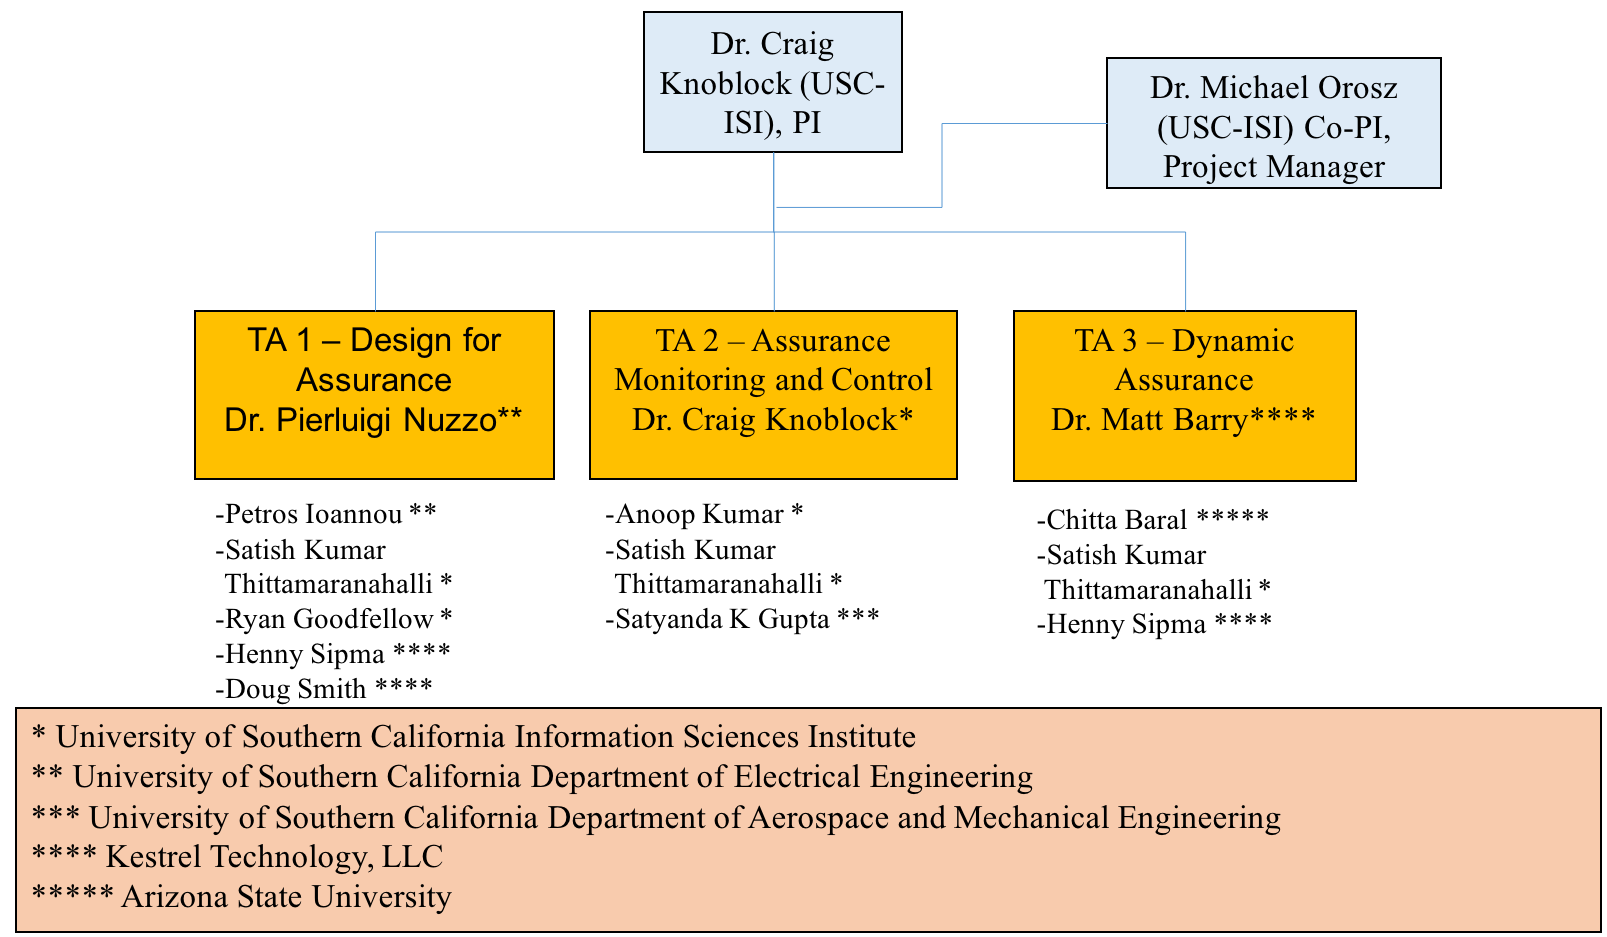
\includegraphics[width=6.0in]{./org-chart2.png}
\caption{\small Organization Chart}
\label{fig:org_chart}
\end{figure}

Coordination: To maximize collaboration and reduce risk to project failure from lack of communication and technical exchange, we plan to employ a wide variety of working styles and communication/coordination so that all can contribute.  At the core of our project will be regularly scheduled meetings bridging the diversely distributed team (Table~\ref{fig:Collaboration_Table}).  These meetings will address project status, identify challenges, implement risk mitigation strategies and participate in technology exchanges and system integration efforts (when appropriate)

\begin{table}[ht]
\caption{\small Project Meetings and Events}
  \centering
  {\footnotesize
\begin{tabular}{|m{3.15in}|m{3in}|} 
\hline
\textbf{Meeting} & \textbf{Frequency} 
\\\hline
Conference calls among investigators (discuss project status, address concerns and project risks) & Weekly
\\
\hline
Technical exchange and coordination meetings using Bluejeans or another videoconference technology & At least twice a month and more frequently as needed
  \\ 
\hline
Face-to-Face meetings (prior to P/I and demonstration meetings) & Every 3 to 6 months and more frequently (especially at the beginning of the project) as needed
 \\\cline{1-2}

\hline
\end{tabular}
}
\label{fig:Collaboration_Table}
\end{table}

\begin{table}[tbhp]
\caption{\small Key Project Team Member Responsibilities}
  \centering
  {\footnotesize
\begin{tabular}{| m{.75in} | m{3.9in}| m{1.5in}|} 
\hline
\textbf{Key Member} & \textbf{Responsibilities} & \textbf{Tasks} 
\\\hline
Dr.\ Craig Knoblock  & Principal Investigator responsible for project, leads TA 2 – Assurance Monitoring and Control.  Will lead the overall project and lead the TA2 team.  Served as the PI on many DARPA projects and has sucessfully led many large teams.    Effort on project:  25\% &
1.1.6, 1.2.2 1.2.3, 1.2.4, 1.3.4, 1.4.1, 
2.1.6, 2.2.2 2.2.3, 2.2.4, 2.3.4, 2.4.1, 
3.1.6, 3.2.2, 3.2.3, 3.2.4, 3.3.4, 3.4.1
\\
\hline
Dr.\ Michael Orosz & Co-Principal Investigator responsible managing the day-to-day operations of the project, assist technical teams as needed, coordinate with TA4 teams.    Has led many large complex multi-disciplined/multi-organizational projects in academic and industry environments.  Effort on project: 50\%
& 1.1.6, 2.1.6, 3.1.6, 1.4.1, 2.4.1, 3.4.1
  \\ 
\hline
Dr.\ Pierluigi Nuzzo 
& 
Co-Principal Investigator.  Leads the TA 1 - Design for Assurance team and conducts research on the formal methods for the design of the TA1 system.  Research experience on methodologies and tools for the design of cyber-physical systems; contracts, interfaces, and compositional methods for embedded system design; the application of automated formal methods and optimization theory to problems in embedded and cyber-physical systems.  Effort on project: 2 months/year (16.6\%)
& 
1.1.1, 2.1.1, 3.1.1 \\
\hline
Dr.\ Matthew Barry
& 
Key personnel.  Leads the TA 3 – Dynamic Assurance.   He will conduct the research on the dynamic assurance case language editors and parsers, the run-time system, and system integrations. Effort on project:  66\%
& 
1.3.2, 2.3.2, 3.3.2\\
\hline
Dr.\ Chitta Baral
& 
Key personnel responsible for learning assurance rules, supporting assurance rules with uncertainty and improving solver speed.  Expertise on ASP solvers, which will be used to reason about the assurance cases. Effort on project: 20\%
& 
1.3.1, 2.3.1, 3.3.1 \\
\hline
Dr.\ Doug Smith 
& 
Key personnel will support formal methods aspects of TA1, and lead the effort on abstract refinement. Expertise in field of automated correct-by-construction program generation.    Effort on project: 40\%
& 
1.1.5, 2.1.5, 3.1.5 \\
\hline
Dr.\ Henny Sipma
& 
Key personnel who will support the program verification tasks under TA1.  Will lead the effort on program verification.   Effort on project:  45\%
& 
1.1.5, 2.1.5, 3.1.5, 1.3.2, 2.3.2, 3.3.2 \\
\hline
Dr.\ Petros Ioannou
& 
Key personnel responsible providing and extending the assurance test bed, which will be available at the start of the project for autonomous vehicles.   Effort on project: 1 month/year (8.3\%)
& 
1.1.2, 2.1.2 (optional), 3.1.2 (optional)
\\
\hline
Dr.\ Satyandra Kumar Gupta
& 
Key Personnel providing autonomous command and control expertise to the TA-2 team.   Will lead the research on safety aware learning on TA2.   Past research on physics-aware decision making to facilitate automation.  Effort on project: 1 month/year (8.3\%)
& 
1.2.1, 2.2.1, 3.2.1 \\
\hline
Dr.\ Anoop Kumar 
& 
Key personnel providing support to the TA 2 project team.  Will lead the research on monitoring \& control and detecting distribution shifts.  Effort on project: 50\%
& 
1.2.1, 1.2.2, 1.2.3, 1.2.4, 2.2.1, 2.2.2, 2.2.3, 2.2.4, 3.2.1, 3.2.2, 3.2.3, 3.2.4\\
\hline
Dr.\ Satish Thittamaranahalli
& 
Key personnel developing scalable algorithms for TA1, TA2, and TA3 project teams.  Has extensive experience on scalable algorithm design, machine learning, and constraint reasoning.  Effort on project: 50\%
& 
1.2.1, 1.2.2, 1.2.3, 1.2.4, 2.2.1, 2.2.2, 2.2.3, 2.2.4, 3.2.1, 3.2.2, 3.2.3, 3.2.4, 1.1.4, 2.1.4, 3.1.4 \\
\hline
Dr.\ Ryan Goodfellow
& 
Key personnel providing support to the TA-1 project. Will lead the research on simulation-based testing.  Has extensive experience on simulation-based testing.  Effort on project:  30\%
& 
1.1.3, 2.1.3, 3.1.3 \\

\cline{1-2}

\hline
\end{tabular}
}
\label{fig:Table_Mgmt}
\end{table}



\newpage
\section{Personnel, Qualifications and Commitment}

{\bf Dr.\ Craig Knoblock}, the PI on this effort, is a Research Professor of both Computer Science and Spatial Sciences at the University of Southern California (USC) and Director of the Intelligent Systems Division at the USC Information Sciences Institute.   He received his Ph.D. from Carnegie Mellon University in computer science. 
%His research focuses on techniques for describing, acquiring, and exploiting the semantics of data.  
In previous projects he has worked on developing  scalable approaches to execution monitoring, accurate detection of sensor failures, and   automatic modeling and reconstruction of sensors.  He has published more than 300 journal articles, book chapters, and conference papers on these topics.  Dr. Knoblock is a Fellow of the Association for the Advancement of Artificial Intelligence (AAAI), a Distinguished Scientist of the Association of Computing Machinery (ACM), a Senior Member of IEEE, past President and Trustee of the International Joint Conference on Artificial Intelligence.
%and winner of the 2014 Robert S. Engelmore Award.  

{\bf Dr.\ Michael Orosz}, a Co-PI on this effort, is a Research Associate Professor of Civil and Environmental Engineering at the University of Southern California (USC) and Research Director of the Decision Systems Group at the USC Information Sciences Institute.  Dr. Orosz has over 30 years’ experience in commercial and government software development, basic and applied research, project management, academic research and has developed and deployed several commercially successful products.  His research interests are in machine learning and decision analytics as applied to intelligence analysis and autonomous command and control such as smart building controls.    Dr. Orosz has extensive experience in managing large complex multi-disciplined/multi-teamed research projects. %funded by DARPA, DHS, DoD, DoE, Industry, NASA, NRO, NSA and ONR.   
He received his Ph.D. in computer science from the University of California, Los Angeles.

{\bf Dr.\ Pierluigi Nuzzo}, a Co-PI on this project, is an Assistant Professor in the Department of Electrical Engineering at the University of Southern California. He received the Ph.D. in Electrical Engineering and Computer Sciences from the University of California at Berkeley. 
%in 2015, and the Laurea degree (MS) in electrical engineering (summa cum laude) from the University of Pisa, Italy, and the Sant'Anna School of Advanced Studies, Pisa, Italy.
%
%He has four years of research experience in analog and mixed signal circuit design as a researcher at IMEC, Leuven, Belgium, and over 10 years experience in design methodologies and tools for mixed-signal integrated circuits and cyber-physical systems, as a researcher at the University of Pisa, IMEC, UC Berkeley, and USC. 
His research interests
include: methodologies and tools for cyber-physical system and mixed-signal
system design; contracts, interfaces and compositional methods for embedded
system design; the application of formal methods and optimization theory to problems in embedded and cyber-physical systems and electronic design automation. 
%
Prof. Nuzzo received %First Place in the operational category and Best Overall
%Submission in the 2006 DAC/ISSCC Design Competition, 
a Marie Curie Fellowship
from the European Union in 2006, 
the University of California at Berkeley EECS
departmental fellowship in 2008, 
%the University of California at Berkeley Outstanding Graduate Student Instructor Award in 2013, 
the IBM Ph.D.
Fellowship in 2012 and 2014, 
%the Best Paper Award from the International Conference on Cyber-Physical Systems (ICCPS) in 2016, 
and the David J.~Sakrison Memorial Prize in 2016 for his doctoral research. 
%He is an author of 1 patent and over 60 publications.

{\bf Dr.\ Satyandra K. Gupta} is Smith International Professor in the Department of Aerospace and Mechanical Engineering at the University of Southern California. %Prior to joining the University of Southern California, he was a Professor in the Department of Mechanical Engineering and the Institute for Systems Research at the University of Maryland. He was the founding director of the Maryland Robotics Center and the Advanced Manufacturing Laboratory at the University of Maryland. 
He served as a program director for the National Robotics Initiative at the National Science Foundation from September 2012 to September 2014.  Dr. Gupta's interest is in the area of physics-aware decision making to facilitate automation. He has published more than 300 technical articles. He is a fellow of the American Society of Mechanical Engineers (ASME) and editor of ASME Journal of Computing and Information Science in Engineering. Dr. Gupta has received the Young Investigator Award from the Office of Naval Research in 2000, CAREER Award from the National Science Foundation in 2001, Presidential Early Career Award for Scientists and Engineers (PECASE) in 2001, Invention of the Year Award at the University of Maryland in 2007, Kos Ishii-Toshiba Award from ASME in 2011, and Excellence in Research Award from ASME in 2013.%, and Distinguished Alumnus Award from Indian Institute of Technology, Roorkee in 2014. %He has also received seven best paper awards at conferences.

{\bf Ryan Goodfellow} is a computer scientist at ISI working in combined cyber physical simulation and emulation platform development. His formal background is in simulation algorithms and modeling techniques using differential-algebraic equations (DAE). He has applied this knowledge in the CPS space by integrating DAE modeling languages and simulation engines with network testbeds to create comprehensive scientific experimentation platforms for cyber-physical systems. These experimentation platforms have been used in the power grid research space. %Ryan is a lead developer on the Deter network testbed, with a strong background in networked and distributed systems engineering. %He is also a combat veteran, serving as a non-commissioned officer and SIGINT team lead for a multi-functional intelligence team in Afghanistan.

{\bf Dr.\ Petros Ioannou} is a Professor in the Department of Electrical Engineering, Director of the Center for Advanced Transportation Technologies and Associate Director for Research for the DOT supported University Transportation Center at USC. He received his MS and PhD from the University of Illinois at Urbana Champaign in Mechanical and Electrical Engineering, respectively. His research interests are in robust adaptive control, vehicle dynamics and control, human factors and safety, automated vehicles, nonlinear systems and Intelligent transportation Systems.  He received the 2016 IEEE Transportation Technologies field award and the 2016 IEEE Control system society Transition to Practice Award. He is a Fellow of IEEE, IFAC and IET and author/coauthor of 8 books and over 400 papers.

{\bf Dr.\ Matthew Barry} will serve as lead for the TA3 tasks. %He will implement the dynamic assurance case language editors and parsers, the run-time system, and system integrations.  He will implement the assurance case arguments and the API for updating argument structure and content.  
Dr. Barry currently is CEO at Kestrel Technology LLC, and previously spent 20 years in NASA space mission operations at the Jet Propulsion Lab and Johnson Space Center.  At NASA Headquarters he led the introduction of dependability case requirements and plans for flight computing systems in upcoming manned space exploration missions, as well as the development of Agency-level software-related safety-critical control system requirements.  He recently served as a Principal Investigator on DHS/Cyber S\&T STAMP (Static Tool Analysis Modernization Program), DARPA CSFV (Crowd Sourced Formal Verification), three NASA Aeronautics R\&D projects, and the AFRL-sponsored Static Analysis of Numerical Algorithms project.  Dr. Barry earned BSME, MS, and PhD degrees in mechanical engineering, and an MBA degree, from Rice University.  

{\bf Dr.\ Henny Sipma} will support the program verification tasks under TA1.  %She is the key person behind the company's {\em KT Advance\/} and {\em KT Transferal\/} static analysis products, and the designer and programmer of the company's core {\em CodeHawk\/} abstract interpretation engine. 
Dr. Sipma currently is the CTO at Kestrel Technology LLC.  She has spent the past 10 years with Kestrel Technology as a static analysis expert; previously developed and taught static analysis techniques as senior research associate at Stanford University for eight years; and developed industrial process controls as an senior systems analyst at Shell.  She has been Principal Investigator or company lead on several recent R\&D projects for Federal agencies, including two projects under the IARPA STONESOUP (Securely Taking On New Executable Software of Uncertain Provenance) program; the DHS Cyber S\&T Gold Standard project; and the DARPA-sponsored STAC (Space-Time Analysis for Cybersecurity) and MUSE (Mining and Understanding Software Enclaves) programs.  Dr. Sipma earned 
%a BS degree in chemistry and an MS degree in chemical engineering at the University of Groningen in The Netherlands, and 
MS and PhD degrees in computer science from Stanford University.  

{\bf Dr.\ Douglas R.\ Smith} will support formal methods aspects of TA1, including the enforcement of safety properties and the generation of monitors.  He is President of Kestrel Technology LLC and Principal Scientist at Kestrel Institute.  He is a Fellow of the American Association of Artificial Intelligence (AAAI) and an ASE Fellow (Automated Software Engineering).  From 1986 to 2000, he taught an advanced graduate course on correct-by-construction software development at Stanford.  
%Dr. Smith has led the development of a series of software synthesis systems, including KIDS (Kestrel Interactive Development System), Specware, Designware, and Planware. 
%Applications domains have included a variety of complex high-performance planners and schedulers for the US Air Force.  He leads current projects on the generation of air mission plans and cyberoperations.  
Other recent projects focused on automated policy enforcement \cite{SmithD0703,SmithD08}, synthesis of secure network protocol codes, and the synthesis of high-performance constraint-solvers\cite{SmithD08c,SmithD13}.  Dr. Smith has over 30 years experience in the field of automated correct-by-construction program generation and has published over 100 papers. He has one patent.  He received the Ph.D. in Computer Science from Duke University% in 1979.  

{\bf Dr. Chitta Baral} is a Professor in the Department of Computer Science and Engineering at Arizona State University. He will support the TA3 efforts on Learning assurance rules, supporting assurance rules with uncertainty and improving solver speed. Dr. Baral has expertise in various aspects of autonomy and Artificial Intelligence. 
He wrote the first book on answer set programming (published by Cambridge University Press) the formal language behind our assurance rules. Some of his other works relevant to this proposal are: goal specification for autonomous systems, automatic construction of control rules for autonomous systems that satisfy given goals, combining machine learning with reasoning in various contexts, including image understanding. %He is the President of KR Inc. He is an associate editor of AIJ and has been an associate editor of JAIR.

{\bf Dr.\ Satish Kumar Thittamaranahalli (T. K. Satish Kumar)} leads the Collaboratory for Algorithmic Techniques and Artificial Intelligence (CATAI) at USC's Information Sciences Institute. He has published over 60 papers on numerous topics in Artificial Intelligence spanning such diverse areas as Constraint Reasoning, Planning and Scheduling, Probabilistic Reasoning, Robotics, Combinatorial Optimization, Approximation and Randomization, Heuristic Search, Model-Based Reasoning, Knowledge Representation and Spatio-Temporal Reasoning. %He %has served on the Program Committees of many international conferences in Artificial Intelligence
He and is a winner of the 2016 Best Robotics Paper Award and the 2005 Best Student Paper Award from the International Conference on Automated Planning and Scheduling. 
Dr. Kumar received his PhD in Computer Science from Stanford University. %In the past, he has also been a Visiting Student at the NASA Ames Research Center, a Postdoctoral Research Scholar at the University of California, Berkeley, a Research Scientist at the Institute for Human and Machine Cognition, a Visiting Assistant Professor at the University of West Florida, and a Senior Research and Development Scientist at Mission Critical Technologies.

\textbf{Dr.\ Anoop Kumar} is a senior computer scientist at USC ISI and has broad expertise in machine learning, statistical modeling, and software engineering.  Dr.\ Kumar is the technical lead on the DARPA RSPACE program and has played a vital role in developing a system that fuses air operations data from multiple sources, maintains world state, and issues warnings. Previously, he led the research and development of the BBN’s election forecasting system for the IARPA OSI program. %Dr.\ Kumar played a significant role in the DARPA DEFT program by developing a model to support integration of output from multiple NLP algorithms. He has contributed at the development to management levels on government research contracts and commercial projects. 
Dr.\ Kumar helped design and develop BBN's commercially available, hosted speech and medical transcription services offering. 

\begin{table}[!tbh]
\begin{footnotesize}
\vspace{-0.1in}

\begin{tabular}{lll}
\begin{tabular}[t]{|l|@{}c@{}|@{}c@{}|@{}c@{}|@{}c@{}|} \hline
Project & Status & \multicolumn{3}{ c| }{Hours} \\ \cline{3-5}
& & P1 & P2 & P3 \\ \hline



\multicolumn{5}{ |c| }{ \textbf{Craig Knoblock} } \\ \cline{1-5}
Safeguard & Pro & 770 & 641 & 641 \\ \cline{1-5}
ELICIT & Cur & 308 & 256 & 120 \\ \cline{1-5}
WTNIC & Cur & 11 & 0 & 0 \\ \cline{1-5}
EFFECT & Cur & 641 & 107 & 0 \\ \cline{1-5}
LinkedMaps & Cur & 203 & 25 & 0 \\ \cline{1-5}
PRINCESS & Cur & 608 & 96 & 0 \\ \cline{1-5}
SCHARP & Cur & 481 & 54 & 0 \\ \cline{1-5}
MINT & Pen & 650 & 534 & 285 \\ \cline{1-5}

\multicolumn{5}{ |c| }{ \textbf{Michael Orosz} } \\ \cline{1-5}
Safeguard & Pro & 1560 & 1300 & 1300  \\ \cline{1-5}
SMC/SY & Cur & 1803 & 0 & 0  \\ \cline{1-5}

\multicolumn{5}{ |c| }{ \textbf{Matthew Barry} } \\ \cline{1-5}
Safeguard & Pro & 2078 & 1690 & 1554 \\ \cline{1-5}
Starlite & Cur & 1840 & 1692 & 0 \\ \cline{1-5}



\multicolumn{5}{ |c| }{ \textbf{Anoop Kumar} } \\ \cline{1-5}
Safeguard & Pro & 1560 & 1300 & 1300 \\ \cline{1-5}

\end{tabular}
&
\begin{tabular}[t]{|l|@{}c@{}|@{}c@{}|@{}c@{}|@{}c@{}|} \hline
Project & Status & \multicolumn{3}{ c| }{Hours} \\ \cline{3-5}
& & P1 & P2 & P3 \\ \hline

\multicolumn{5}{ |c| }{ \textbf{Pierluigi Nuzzo} } \\ \cline{1-5}
Safeguard & Pro & 520 & 433 & 433  \\ \cline{1-5}
Mirage & Cur & 433 & 0 & 0  \\ \cline{1-5}

\multicolumn{5}{ |c| }{ \textbf{Satyandra Gupta} } \\ \cline{1-5}
Safeguard & Pro & 260 & 217 & 217 \\ \cline{1-5}
Human   & Cur & 22 & 0 & 0 \\ \cline{1-5}
Vehicles & Cur & 36 & 0 & 0 \\ \cline{1-5}
Robot & Cur & 116 & 0 & 0 \\ \cline{1-5}
Assembly & Cur & 33 & 0 & 0 \\ \cline{1-5}
Solar & Cur & 4 & 0 & 0 \\ \cline{1-5}

\multicolumn{5}{ |c| }{ \textbf{Petros Ioannou} } \\ \cline{1-5}
Safeguard & Pro & 260 & 217 & 217 \\ \cline{1-5}
CPS & Cur & 130 & 0 & 0 \\ \cline{1-5}

\multicolumn{5}{ |c| }{ \textbf{Ryan Goodfellow} } \\ \cline{1-5}
Safeguard & Pro & 936 & 780 & 780 \\ \cline{1-5}
STEAM & Cur & 416 & 0 & 0 \\ \cline{1-5}


\end{tabular}
&
\begin{tabular}[t]{|l|@{}c@{}|@{}c@{}|@{}c@{}|@{}c@{}|} \hline
Project & Status & \multicolumn{3}{ c| }{Hours} \\ \cline{3-5}
& & P1 & P2 & P3 \\ \hline

\multicolumn{5}{ |c| }{ \textbf{Chitta Baral} } \\ \cline{1-5}
Safeguard & Pro & 659 & 485 & 485 \\ \cline{1-5}
PostdocBP & Cur & 176 & 0 & 0 \\ \cline{1-5}
Languages & Pen & 528 & 264 & 264 \\ \cline{1-5}
CAREER & Pen & 88 & 44 & 44 \\ \cline{1-5}
CHS & Pen & 510 & 255 & 0 \\ \cline{1-5}

\multicolumn{5}{ |c| }{ \textbf{Doug Smith} } \\ \cline{1-5}
Safeguard & Pro & 1222 & 984 & 840 \\ \cline{1-5}
RSPACE & Cur & 342 & 0 & 0 \\ 
\cline{1-5}
PLANX & Cur & 154 & 0 & 0 \\ 
\cline{1-5}
HACCS & Pen & 923 & 769 & 769 \\ 
\cline{1-5}

\multicolumn{5}{ |c| }{ \textbf{Henny Sipma} } \\ \cline{1-5}
Safeguard & Pro & 1372 & 962 & 840 \\ \cline{1-5}
STAC & Cur & 797 & 0 & 0 \\ \cline{1-5}

\multicolumn{5}{ |c| }{ \textbf{Satish Thittamaranahalli} } \\ \cline{1-5}
Safeguard & Pro & 1560 & 1300 & 1300 \\ \cline{1-5}
MapF & Cur & 103 & 103 & 0 \\ \cline{1-5}

\end{tabular}
\end{tabular}

\end{footnotesize}
\caption{Individual commitments of key personnel}
\label{tab:Commitments}
\vspace{-0.2in}
\end{table}

\clearpage
\newpage
\section{Capabilities}


%\subsection{University of Southern California}
USC has strengths in number of areas that are closely related to the proposed work:
\begin{itemize}[itemsep=0pt,leftmargin=*]
\item Dr.\ Nuzzo 
%has over 10-year research experience in embedded system design, from mixed-signal chip design (analog-to-digital converters, frequency synthesizers, software-defined radio), to methodologies and tools for mixed-signal integrated circuits and Cyber-Physical Systems (CPSs), and the application of formal methods and optimization theory to problems in embedded and cyber-physical systems and electronic design automation.  
%His doctoral work 
has done extensive research on contracts and compositional methods for heterogeneous system design and design space exploration, with application to aircraft electric power systems and environmental control systems. His work has helped transition rigorous system design foundations, innovative design methodologies, and new systems engineering paradigms to industry (IBM, United Technologies). 
\item Dr.\ Satyandra K. Gupta has worked on autonomous surface vehicles, autonomous ground vehicles for operation on rugged terrains, and autonomous flapping wing aerial vehicles.   His group has developed a hierarchal decision making approach for realizing autonomous systems. 
%This approach combines task planning and assignment, deliberative trajectory planning, reactive collision avoidance behaviors, and trajectory tracking control layers. 
His group has also developed new methods for learning reactive behaviors in adversarial environments and COLREGS compliant trajectory planning. \item Dr.\ Knoblock has developed methods that learn the relationships between sensors to both identify failures and changes in sensor and reconstruct those sensors, providing estimates of the accuracy of the reconstructed sensors.  
\item Ryan Goodfellow has extensive experience in simulation based testing through high-fidelity CPS testbed environment development and operation, using the Deter network testbed as the core which has supported several large scale government projects from a variety of agencies and thousands of users. %we have developed sophisticated CPS experiments under programs such as NFS RIPS, NIST SmartCities and the DHS Cybersecurity showcase.
\item Dr.\ Ioannou %helped  design and implement adaptive cruise control systems in collaboration with Ford Motor Company, which was commercialized four years before any other company. He 
worked on several DOT funded projects on automated vehicles and intelligent highway systems where he demonstrated his vehicle control designs for safety and performance on actual automated vehicles in test trucks and I-15 highway.
\item Drs.\ Knoblock, Kumar, and Thittamaranahalli have developed highly scalable approaches for monitoring message traffic to identify potential problems and issue warnings and alerts. 
\item Dr. Thittamaranahalli has developed state-of-the-art methods for efficiently solving large-scale search and optimization problems. %These techniques will be applicable in TA2 for safety-aware learning and planning, in TA2 for assurance monitoring and control, and in TA3 for dynamic assessment of assurance cases.

\end{itemize}
%\subsection{Kestrel Technology LLC}

Kestrel Technology's strength is in program analysis, specifically static analysis of both source and binary targets.  The company performs applied R\&D and product development for a variety of static analysis applications  pivoting primarily on the abstract interpretation technique.  The company recently initiated development of program analysis applications using logical equivalence techniques. As a provider of verification evidence in the form of mathematical proofs, the company also has expertise in the design and development of assurance case arguments for high-integrity systems using such evidence. %The company is engaged in a partnership with Wind River Systems to develop program analysis tools for its embedded system developers.  Many of Wind River's customers must develop their products under safety and certification standards, including those using safety cases.  

   

%\subsection{Arizona State University}
Chitta Baral at Arizona State University has developed various software to learn assurance rules and various ASP solvers, which he has made available as open-source.

Most of the software carried forward for implementation or derivation is open source.  The single exception is Kestrel Technology's {\it KT Advance\/} static analysis tool (TA1), in particular the abstract interpretation engine therein, which is company proprietary and is US EAR export-controlled.   
%Owing to mixed funding for the development of that technology 
We will continue to provide the Federal government a restricted use license for that particular item.

There are no specialized facilities, data, or GFE required for this effort. 

\include{sow}
\include{milestones}

% \section{Level of Effort by Task \textcolor{red}{[Mike/Lisa - 1 pages]}}

% \textcolor{blue}{
% \begin{itemize}
% \item Will be a separate spreadsheet
% \item
% \end{itemize}
% }

\include{appendix_a}

%\section{Appendix B \textcolor{red}{[No Page Count]}}

\section{References}
\bibliographystyle{acm} 
\bibliography{TA3/ta3,TA2/ta2,TA1/ta1}
\end{document}
%%\documentclass[a4paper]{article}
%\documentclass[12pt]{article}
\documentclass[12pt]{dod-blank}

%% Language and font encodings
\usepackage[english]{babel}
\usepackage[utf8x]{inputenc}
\usepackage[T1]{fontenc}

%% Sets page size and margins
%%\usepackage[a4paper,top=3cm,bottom=2cm,left=3cm,right=3cm,marginparwidth=1.75cm]{geometry}
%\usepackage[top=1in, bottom=1in, left=1in, right=1in]{geometry}



%% Useful packages
\usepackage{amsmath}
\usepackage{graphicx}
  \graphicspath{{.}{./image/}}
  \DeclareGraphicsExtensions{.png,.jpg} 
\usepackage[colorinlistoftodos]{todonotes}
\usepackage[colorlinks=true, allcolors=blue]{hyperref}
\usepackage{tabularx}
\usepackage{multirow}
\usepackage{tabulary}
\usepackage{float}
\usepackage{wrapfig}
\usepackage[export]{adjustbox}
\usepackage{comment}
\usepackage{tabularx}
\usepackage{multirow}
\usepackage{tabulary}
\usepackage{enumitem}

\usepackage{listings}
\usepackage{color}
\usepackage{array}
\usepackage{subcaption}
\usepackage{xcolor}




\renewcommand{\textfraction}{0}
\renewcommand{\topfraction}{1.0}
\renewcommand{\bottomfraction}{1.0}

\usepackage{longtable}
%% macros
\newif\iffinal
\finaltrue
\iffinal
  
    \newcommand\baareq[1]{}
    \newcommand\baades[1]{}
 
 
\else
    \definecolor{darkgreen}{rgb}{0,0.4,0}
    \definecolor{darkcyan}{rgb}{0,0.4,0.4}
    \definecolor{darkblue}{rgb}{0,0,0.5}
    
    \newcommand\baareq[1]{{\color{darkcyan}[\textbf{Requirement:} #1]}}
    \newcommand\baades[1]{{\color{darkcyan}[\textbf{Description:} #1]}}
 
\fi




\def\naive{na\"{\i}ve}



\lstset{ 
  backgroundcolor=\color{white},   % choose the background color; you must add \usepackage{color} or \usepackage{xcolor}
  basicstyle=\footnotesize\ttfamily,            % the size of the fonts that are used for the code
  breakatwhitespace=false,         % sets if automatic breaks should only happen at whitespace
  breaklines=true,                 % sets automatic line breaking
  captionpos=b,                    % sets the caption-position to bottom
  commentstyle=\color{mygreen},    % comment style
  % deletekeywords={...},            % if you want to delete keywords from the given language
  escapeinside={\%*}{*)},          % if you want to add LaTeX within your code
  extendedchars=true,              % lets you use non-ASCII characters; for 8-bits encodings only, does not work with UTF-8
  frame=single,	                   % adds a frame around the code
  keepspaces=false,                 % keeps spaces in text, useful for keeping indentation of code (possibly needs columns=flexible)
  keywordstyle=\color{blue}\bfseries\underbar,       % keyword style
  language=Prolog,                 % the language of the code
  % morekeywords={if,and},        % if you want to add more keywords to the set
  numbers=none,                    % where to put the line-numbers; possible values are (none, left, right)
  numbersep=5pt,                   % how far the line-numbers are from the code
  numberstyle=\tiny\color{mygray}, % the style that is used for the line-numbers
  rulecolor=\color{black},         % if not set, the frame-color may be changed on line-breaks within not-black text
  showspaces=false,                % show spaces everywhere adding particular underscores; it overrides 'showstringspaces'
  showstringspaces=false,          % underline spaces within strings only
  showtabs=false,                  % show tabs within strings adding particular underscores
  stepnumber=2,                    % the step between two line-numbers. If it's 1, each line will be numbered
  stringstyle=\color{mymauve},     % string literal style
  tabsize=2,	                   % sets default tabsize to 2 spaces
  title=\lstname                   % show the filename of files included with \lstinputlisting; also try caption instead of title
}

% apply trick for additional keywords for our AC DSL
\lstset{
	emph={for, if, and, or},
    emphstyle={\color{blue}\bfseries\underbar}
}




\title{DARPA Assured Autonomy}
\author{Technical Volume- \textcolor{red}{Thirty-Eight (38) pages max}}

\begin{document}
\pagenumbering{roman}
\include{cover}

\newpage
\section{Table of Contents}
\tableofcontents

\newpage
\pagenumbering{arabic}
\section{Executive Summary}
As we rapidly move into a world where machine learning plays a central role in realizing autonomous systems, it is becoming increasingly important to develop techniques that assure that these systems will operate safely and perform as expected. Current approaches are limited to providing assurance for systems with limited or no  learning capabilities. In this context, DARPA's Assured Autonomy BAA seeks to \emph{develop rigorous design and analysis technologies for continual assurance of learning-enabled autonomous systems}. USC in collaboration with Kestrel Technology and ASU is pleased to submit a comprehensive TA1, TA2, and TA3 proposal entitled \emph{``Assured Autonomy for Learning Enabled Vehicles (Safeguard).''} We plan to provide an end-to-end solution to support autonomous systems with learning-enabled components, ranging from design technologies for assurance, to assurance monitoring and control techniques, to representation and online evaluation of assurance cases. We have assembled a strong team of experts that cover the range of technologies that are required to create such an end-to-end system. If successful, the project will provide the technologies for building the next-generation of learning-enabled autonomous systems.  The entire project will take four years and cost \textcolor{red}{\$??}, with an initial version completed at the end of Phase I and successive versions with additional capabilities and improved scalability at the end of Phase II and Phase III.  

In the remainder of this section, we first introduce an  unmanned surface vehicle scenario that will be used throughout the proposal to describe the approach.  Next, we describe our approach to design, monitoring, and dynamic assurance. Finally, we introduce the team involved in the project. 

\textbf{Motivating Scenario.} Consider an autonomous unmanned surface vehicle (USV) guarding a valuable asset in the ocean when an unknown vehicle  approaches the security perimeter, under challenging weather conditions. In this scenario, the USV is required to approach the intruding vehicle, issue a warning signal, and escort it to a safe distance from the controlled area. However, as the USV has no a priori knowledge of its external environment behaviors (e.g., water depth, waves, wind, current, visibility), pre-computing a feasible trajectory, let alone optimal, becomes a non-trivial problem. For trajectory planning, the USV must continuously perform the following tasks:
\begin{itemize}[itemsep=0pt,leftmargin=*]
 \item Sense the current state of the surrounding environment (e.g., water depth, waves, wind, current, visibility) and estimate its own maneuverability constraints (e.g., braking distance, available acceleration, maximum velocity, turning radius, turning rate, safety distance) based on the state of the environment;      
\item Sense the static obstacles in the sensor range and generate a traversability map;
\item Sense the moving obstacles and classify them;   
\item Predict future trajectories of moving obstacles; 
\item Determine if any of the COLREGS \cite{commandant1999international} rules will be in effect with respect to one or more of the nearby vessels and identify the vessels with the right of way.    
\end{itemize}
The above information will be used by the trajectory planner to compute an initial trajectory, which will be continuously refined as the USV gathers additional information.
% It is not possible for the USV to be tested in every possible environment. 
The USV will use learning enabled components to take  decisions as it encounters new situations, such as  
\begin{itemize}[itemsep=0pt,leftmargin=*]
\item Classifiers to identify moving obstacles based on physical appearance and motion signatures,
\item Algorithms to estimate the sensor capabilities in adverse weather conditions,   
\item Algorithms to accurately estimate uncertainty in the environment, 
\item Classifiers to generate traversability maps,
\item Prediction of external vessel behaviors based on motion histories, 
\item Reinforcement learning  to ensure COLREGS compliance of maneuvers,  
\item Algorithms to learning pursuit behaviors.  
\end{itemize}
Learning enabled components will interact with each other in complex ways, where a misclassification error in one component may eventually compromise the entire mission.   
% We will need to make sure that each learning enabled components has a run-time monitor that will ensure that the assumptions made by the learning-enabled component remain valid and prevent erroneous learning. 
% For example, if the vehicle is exhibiting significant error in trajectory tracking, then simply downgrading the trajectory tracking error value may not be a good option.  The failure of prediction of trajectory tracking error might be due to the presence of a significant wake caused by a nearby vessel. The presence of the nearby vessel can be used to explain the degradation in trajectory tracking performance. As the vessel moves away, we can expect the trajectory tracking performance to return to the predicted level.  
While exhaustive validation of learning-enabled cyber-physical systems (LE-CPSs) is a prohibitive task~\cite{Kalra16},
their complexity, heterogeneity, and highly dynamic nature
make it challenging to even leverage existing model-based development techniques to effectively assess system correctness 
% dependability, 
at design time or enforce it at runtime.

\textbf{Design for Assurance.} Safeguard uses a platform-based design approach~\cite{Nuzzo15b} to organize the design process for a LE-CPS and to build assurance cases. Composite models are developed at several levels of abstraction,
from top-level system requirements and safety constraints down to the
implementation level.  Intermediate levels add detail to the levels
above.  The different levels are connected by refinement mappings that
allow properties established at one level to be preserved at the next
level (see Figures~\ref{fig:methodology} and~\ref{fig:assurance}).

Contracts are used to formally specify components and composite models
in terms of (1) Assumptions -- the assumed behaviors of the
environment and the behaviors of other components, and (2) Guarantees
-- the behavior properties that a model guarantees if it operates in a
context that satisfies its assumptions.  A calculus of contracts
allows horizontal composition of contracts to generate contracts for
composite models.  Vertical contracts are used to specify the mapping
or refinement relation between models at different levels of
abstraction.  The system design process starts with a high-level
contract that expresses overall system assumptions and requirements.
Subsequent levels express models with increasing detail until the
lowest level expresses the system in terms of hardware components and
their software controllers.

The assurance case for a CPS arises from the horizontal and vertical
structure of the design in several ways.  The components used within a
particular level are either (1) synthesized using
correct-by-construction design tools together with proofs, (2) derived
statically or dynamically using safety-aware machine-learning
techniques, (3) written manually and verified by analysis tools, or
(4) written manually and validated by extensive testing.  The
assurance case for the whole reflects its compositional structure.  We
anticipate that well-specified contracts together with the calculus of
contracts will eliminate well-known problems with unexpected emergent
behaviors in CPS systems.

The assurance case for the lowest-layer design arises from both the
intra-level assurance and from properties and their proofs that are
preserved under the refinement mapping from the top-level
requirements.  The refinement mappings between model layers will be
constructed using a variety of techniques.  A contract at an abstract
level can be mapped to a component or refined contract by (1)
retrieval of pre-verified components from a platform library, (2)
synthesis using correct-by-construction design and optimization tools,
or (3) manual coding to satisfy a contract.  The mapping of a
composite model will be composed from the mappings of its constituent
components or contracts.  When a composite model cannot be mapped
compositionally to the next level, it will be generated using
correct-by-construction design and optimization tools.

\textbf{Assurance Monitoring and Control.}
We provide an integrated framework for safety-aware learning, assurance monitoring and control, detecting distribution shifts. Three major components offer an efficient TA2 architecture as well as interfaces with TA1 and TA3, that is, (a) safety-aware learning and planning, (b) assurance monitors for guarding architectural and safety constraints; and (c) distribution shift detection.

We will develop a new learning-enabled online decision-making framework that allows opportunistically composing a sequence of actions (maneuvers) to reduce uncertainty in the system capability model without suspending the progress toward the mission goals or compromising safety. Each candidate action is evaluated based on three criteria: (1) the risk of violating a safety constraint using the current uncertainties in the parameter estimates; (2) its relevance to the mission goals; (3)  its expected information gain, i.e., reduction in uncertainty, with respect to the parameter estimates. These evaluations are combined to produce a cumulative mission utility value for each action that drives our learning-enabled decision-making framework. The problem of generating and evaluating sequences of actions can be posed in several way. For example, it can be solved using a branch-and-bound search method like Anytime A*, or formulated with the finite-horizon Markov Decision Process (MDP) framework. We will develop new scalable search strategies to solve this problem efficiently, by potentially evaluating a recent method developed at USC, called FastMap, that can significantly improve the execution time. 

We will develop monitors for architectural and safety constraints. 
% While these constraints can be checked over and over again as sensor information flow in, this naive strategy accounts for a lot of computational overhead. 
To achieve scalability and decrease the overhead, we propose the application of a technique that we currently use in DARPA's RSPACE program, which leverages a physical model of the vehicles dynamics and its interactions with the environment to efficiently determine the readout frequency. We propose two  extensions of this basic idea. First, we will use the theory of Variable Elimination to prioritize which variables to monitor, e.g., controllable, versus uncontrollable, adversarially controlled, or unobservable variables. Second, we invoke the dynamic assessment of assurance cases only when needed. This  decreases the number of times dynamic assessment of assurance cases is initiated as well as the communication bandwidth between the TA2 and TA3 components.

Finally, we will identify a distribution shift by combining statistical and machine learning techniques to differentiate between environmental and sensor changes. We will exploit a categorization of the shifts based on their cause and duration as well as extend our earlier work on detecting and mitigating sensor failures for all types of monitored variables.  

\textbf{Dynamic Assurance:} The Safeguard {\em design for assurance\/} activity takes a systems-theoretic stance toward safety.  Consequently, it presumes that safety is an emergent property of the system, and that hazards can present themselves through unintended interactions and performance violations in addition to causal events such as component failures.  Our design approach includes consideration of intent as well as hazard analysis and mitigation.  The artifacts from these activities populate contracts and assumptions for the dynamic assurance case.  
We thus build safety into the product by working at a systems-level viewpoint, using lexicon and design patterns familiar to both hardware and software engineers; safety is an emergent property of the system, not an afterthought.  
As system behavior evolves during runtime owing to learning, threats, degradation, or some other factor, the dynamic assurance case identifies whether the safety constraints continue to be satisfied.  If not, it provides notifications or issues recovery instructions directly from a lookup table.

Our implementation of the dynamic assurance case employs a declarative knowledge base inference engine and a domain-specific language tailored to our approach.  We have used them successfully for assurance case tool sets and arguments, and will extend them to reason about uncertainty and learning.  Our approach to achieve scalability is to specialize solvers toward modularity and to take advantage of domain knowledge.  Specifically, we will develop answer set programming techniques for context-dependent learning for reasoning about the learning-enabled components as well as learning assurance rules.  We will develop new formalisms for uncertainty to include causality, using weights for computing probabilities, and probabilistic non-monotonicity.  To achieve scaling objectives we will implement specializations using modularity, weighted CSPs, and message passing. 

% The system safety constraints revealed from that design become the key elements of our dynamic assurance case.  Our verification tools ensure the constraints are relevant, identifiable, and their implementation and effect observable.  

\textbf{Team.} We have assembled a team that is exceptionally well-qualified to build the proposed Safeguard system.  The team will be led by Dr.\ Craig Knoblock, the Principal Investigator for the effort, who currently leads the Intelligent Systems Division at the Information Sciences Institute.  He has led many large DARPA and IARPA projects over the years and has a strong track record in conducting leading edge research and then transitioning the technology to commercial use.  He will be supported by Dr.\ Michael Orosz as the Project Manager, who also has  experience in managing large research projects and on autonomous systems.  The TA1 team will be led by Dr.\ Pierluigi Nuzzo, who is an expert in embedded system design methodologies and the  application of formal methods to cyber-physical systems.  The TA1 team also includes Dr.\ Doug Smith, who has spent many years working on scalable correct-by-construction techniques and Dr.\ Henny Sipma, who has significant experience in applying program verification methods to real-world problems.  The TA1 team also includes Ryan Goodfellow, who has done a large amount of work on simulation-based testing.  The TA2 team will be led by Dr.\ Knoblock who has worked on topics related to both monitoring and detecting distribution changes.  He will be supported by Dr.\ Satyandra Gupta, who is an expert on autonomous surface vehicles as well as on safety-aware learning. He will also be supported by Drs.\ Anoop Kumar and Satish Thittamaranahalli, who have also previously worked on efficient methods for execution monitoring.  The TA3 team will be lead by Dr.\ Matthew Barry, who has experience in creating the technologies for assurance cases.  He will be supported by Dr.\ Chitta Baral, who is an expert on ASP solvers and by Dr.\ Thittamaranahalli who is an expert on SAT solvers, both of which will be applied to provide scalable assurance case reasoning.  Finally, Dr.\ Petros Ioannou, who is an expert on control systems for autonomous vehicles will provide an autonomous vehicle platform, which will form the focus of our work until the TA4 teams provide additional vehicle platforms for development.  

\newpage
\section{Innovative Claims and Deliverables}

In this project we will develop and build an end-to-end system for assured autonomy.  This section describes the key innovations by technical area and then the overall deliverables of the project.

\paragraph{Design for Assurance}

\begin{itemize}[itemsep=0pt,leftmargin=*]
\item We address the LE-CPS design challenges via a holistic approach that can contextually generate design artifacts and assurance cases. We develop a compositional, contract-based modeling framework, methods, and tools to support the design process from system-level requirement capture,  formalization, and analysis, to the generation, testing, and continual monitoring of software and hardware artifacts in feedback loop with a physical process.

\item We develop compositional abstractions and interfaces (vertical contracts) that can  bridge heterogeneous formalisms and heterogeneous decomposition architectures to make system analysis and synthesis tractable, consistently combine different verification and synthesis methods at design time, and provide seamless support for dynamic assurance at run time. %We aim to quantitatively capture the confidence in the satisfaction of requirements under uncertain or unknown conditions, and resilience properties of  systems at different abstraction levels, to enable trade-off evaluation between resilience, performance, and cost.

\item We develop a unifying framework and efficient algorithms to reason about the combination of discrete and continuous dynamics and constraints in the presence of uncertainties in LE-CPS using a satisfiability modulo convex approach~\cite{Shoukry2017} for contract-based system verification and scalable trajectory planning.  

\item We provide an environment for high-fidelity CPS testing, in which production-ready software, e.g.,  safety-critical learning and control, may be deployed and tested 
% by extending the Cypress testbed environment \cite{Goodfellow2015Cypress:Systems} 
with time dilation facilities, so that it synchronizes with a physical simulation that is not necessarily running in real time, while still having the perception of real time.

\item We 
% These facilities allow a cyber system to be  
propose an approach for unanticipated behavior space identification and test coverage maximization which leverages results from the theory of differential algebraic equation (DAE)~\cite{Berger2013ControllabilitySurvey,Ilchmann2005ATheory,BergerOnSystems,Lamour2013} 
to prune the behavior search space and identify smaller regions of interest for efficient simulation-based testing. 
% We then compute the intersection of these two behavior spaces and restrict our simulation based testing search space to this subspace.
\end{itemize}

\paragraph{Assurance Monitoring and Control}

\begin{itemize}[itemsep=0pt,leftmargin=*]
\item 
%We integrate safety-aware learning into the overall decision making problem. The goal is to maximize mission utility without violating the safety constraints. 
Our safety-aware learning framework enables the system to opportunistically select and execute actions to assist the learning-enabled component in reducing model uncertainty without compromising safety or deviating from the mission goals. The value of uncertainty reduction is explicitly incorporated in the optimization process for selecting the best action.  
\item For safety-aware learning, we propose the idea of preprocessing the search space of the problem domain before queries and observations come in. With such a linear-time preprocessing phase, the performance of search and optimization algorithms can be significantly boosted. For example, in regular A* search, the intensional or extensional search space can be preprocessed in near-linear time to yield an embedding of each state as a point in Euclidean space~\cite{cujakk}. Then, when the query comes in, A* search can make use of these Euclidean distances as heuristic distances between two states to yield order-of-magnitude speedups. 
%In Anytime A* for safety-aware learning and planning, this leads to a significantly better quality of actions chosen within a time limit, and in the MDP framework, the same ideas can be used to improve the convergence of Bellman updates for safety-aware Reinforcement Learning.
\item As massive amounts of sensor information flow in, it is imperative for us to efficiently process this information for monitoring architectural and safety constraints. Building on our past work on similar tasks, we propose novel technologies for efficiently monitoring constraints. These algorithms can yield an exponential reduction in the amount of sensor data that needs to be processed. Doing this also reduces the message complexities between the various modules. %We also propose to use the theory of Variable Elimination (VE) to monitor constraints with uncontrollable, adversarially controlled, and/or unobservable variables. VE yields a substrate constraint to monitor that characterizes a dominant strategy of the controllable variables over the uncontrollable, adversarially controlled, and/or unobservable variables.
\item We will develop techniques to identify  distributional shifts and determine the underlying cause (e.g., change in environment, sensor failure,   etc.), as well as strategies for handling the various distributional shifts.   Notably, we propose to build on our past work and use compact representations to exploit historical data to identify distributional shifts.
\end{itemize}

\paragraph{Dynamic Assurance}

\begin{itemize}[itemsep=0pt,leftmargin=*]

\item We demonstrate the integration of dynamic assurance for safety-critical learning-enabled dynamic systems in which evolutionary behaviors are expected and tolerated as a property of the functionality.   The impact will be consequential contributions safety-critical dynamic systems in which evolutionary behaviors are expected and tolerated as portion of the functionality.   
\item We implement dynamic assurance by combining features of system safety, formal methods, logic programming, uncertain reasoning, and domain-specific languages.  We populate assurance case arguments at several levels of modeling and implementation abstraction, using the analysis results to produce design-time evidence supporting assurance claims.  
%We provide automated reasoning about the assurance case itself to produce verification, consistency, and completeness results for the argument.  Dynamic assurance results then yield trusted explanations of whether safety constraints and assumptions and other contracts still hold during the collection of runtime evidence from monitors. 
\item We develop and demonstrate ASP formalisms crucial to applications in dynamic assurance. We demonstrate the suitability of the technology especially for assurance case arguments owing to the improved legibility, consistency and completeness checks, handling of uncertain and default reasoning, and scalability.  
%We will produce modularized solvers for enhanced performance based on recent algorithmic developments in exploiting structure, kernelization, and message passing. We provide a formalism to enable learning of assurance rules. 
We provide a novel approach to handling uncertainty that provides the ability to do causal and counter-factual reasoning as well as probabilistic non-monotonicity.  Overcoming limitations of traditional inductive logic techniques, we develop a novel iterative and incremental approach based on context dependent learning. 
\end{itemize}

\paragraph{Deliverables}
During the course of this project, we will build and deliver a fully-operational system that covers all three of the technical areas.  The detailed capabilities of this system are described in the individual technical sections.  The resulting system will be available as open source under a permissive license, which will allow other organizations to use the work, extend it in new directions, and even commercialize the software.  Kestrel Technology has significant experience in this space and has built and applied these types of technologies to a variety of real world tasks.  Kestrel is ideally suited to pursue commercial uses of this technology and the permissive license will facilitate exploring these opportunities since there will be no need to negotiate intellectual property rights.  

\newpage
\section{Technical Plan}
\input{./TA1/main}
\input{./TA2/main}
\input{./TA3/main}
\clearpage
\newpage


\section{Management Plan}


The Principal Investigator for this effort is Dr. Craig Knoblock who is responsible for all aspects of the effort, will coordinate the parallel team efforts, and will ensure high levels of performance from individual team members.  The Co-P/I, Dr. Michael Orosz, will provide project management and will assist all performers in the execution of the project.    The project team is divided into three working groups (Figure~\ref{fig:org_chart}) corresponding to Technical Areas 1-3, however, members of each team contribute across all project activities.   Table~\ref{fig:Table_Mgmt} defines the major contributions of each project team member to the project tasks.

\begin{figure}[tbhp]
%\vspace{-25pt}
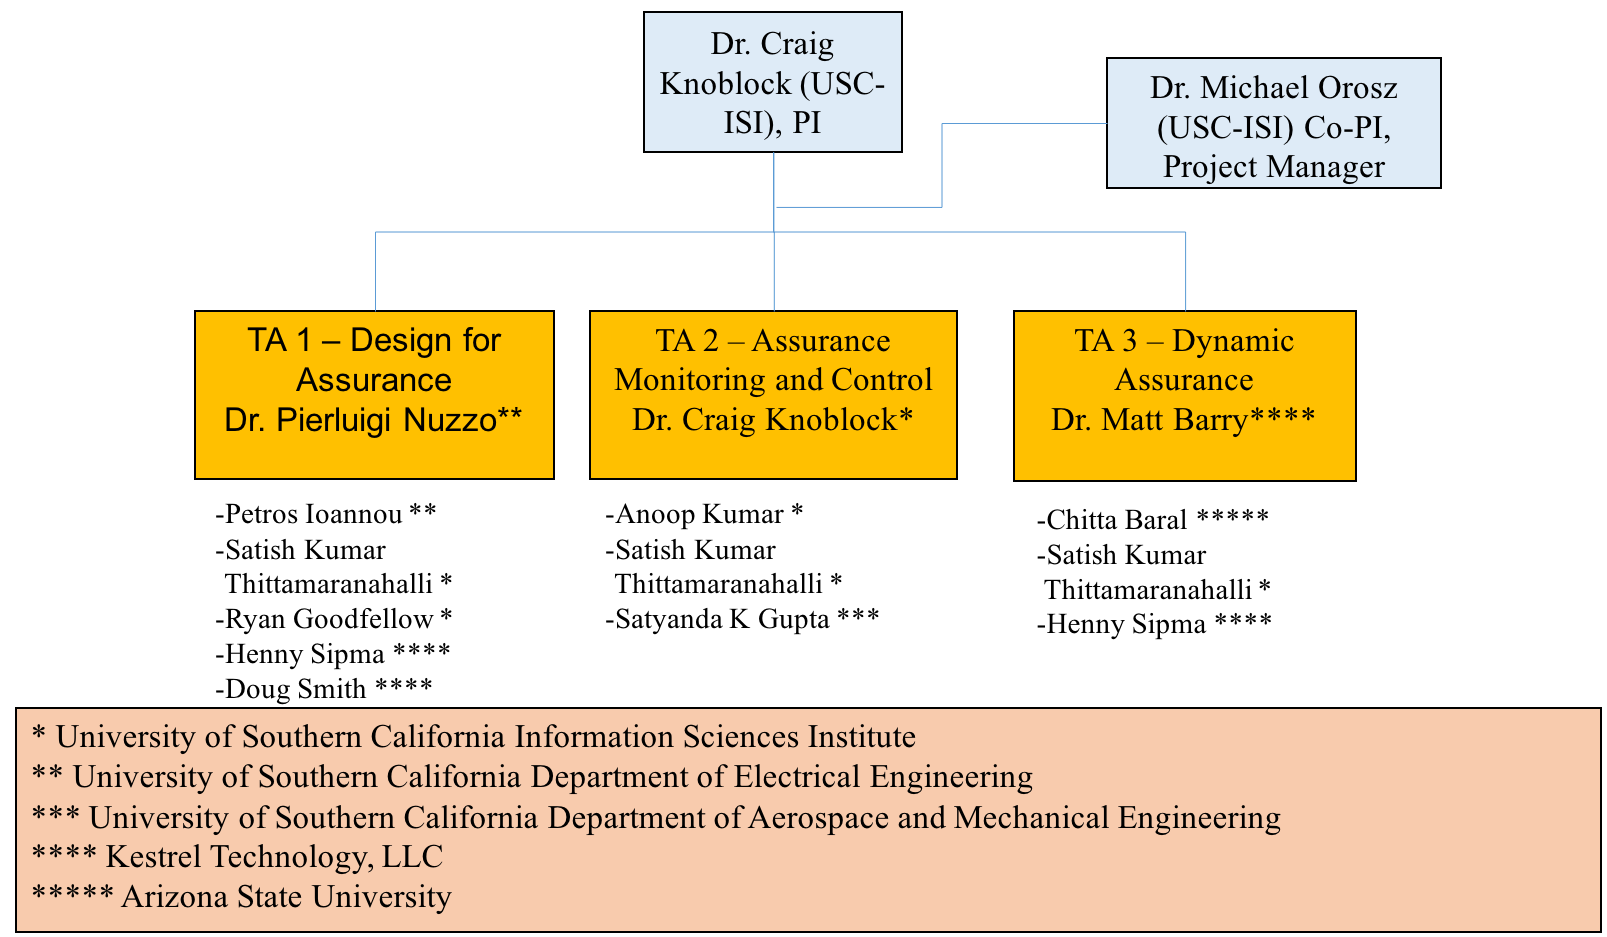
\includegraphics[width=6.0in]{./org-chart2.png}
\caption{\small Organization Chart}
\label{fig:org_chart}
\end{figure}

Coordination: To maximize collaboration and reduce risk to project failure from lack of communication and technical exchange, we plan to employ a wide variety of working styles and communication/coordination so that all can contribute.  At the core of our project will be regularly scheduled meetings bridging the diversely distributed team (Table~\ref{fig:Collaboration_Table}).  These meetings will address project status, identify challenges, implement risk mitigation strategies and participate in technology exchanges and system integration efforts (when appropriate)

\begin{table}[ht]
\caption{\small Project Meetings and Events}
  \centering
  {\footnotesize
\begin{tabular}{|m{3.15in}|m{3in}|} 
\hline
\textbf{Meeting} & \textbf{Frequency} 
\\\hline
Conference calls among investigators (discuss project status, address concerns and project risks) & Weekly
\\
\hline
Technical exchange and coordination meetings using Bluejeans or another videoconference technology & At least twice a month and more frequently as needed
  \\ 
\hline
Face-to-Face meetings (prior to P/I and demonstration meetings) & Every 3 to 6 months and more frequently (especially at the beginning of the project) as needed
 \\\cline{1-2}

\hline
\end{tabular}
}
\label{fig:Collaboration_Table}
\end{table}

\begin{table}[tbhp]
\caption{\small Key Project Team Member Responsibilities}
  \centering
  {\footnotesize
\begin{tabular}{| m{.75in} | m{3.9in}| m{1.5in}|} 
\hline
\textbf{Key Member} & \textbf{Responsibilities} & \textbf{Tasks} 
\\\hline
Dr.\ Craig Knoblock  & Principal Investigator responsible for project, leads TA 2 – Assurance Monitoring and Control.  Will lead the overall project and lead the TA2 team.  Served as the PI on many DARPA projects and has sucessfully led many large teams.    Effort on project:  25\% &
1.1.6, 1.2.2 1.2.3, 1.2.4, 1.3.4, 1.4.1, 
2.1.6, 2.2.2 2.2.3, 2.2.4, 2.3.4, 2.4.1, 
3.1.6, 3.2.2, 3.2.3, 3.2.4, 3.3.4, 3.4.1
\\
\hline
Dr.\ Michael Orosz & Co-Principal Investigator responsible managing the day-to-day operations of the project, assist technical teams as needed, coordinate with TA4 teams.    Has led many large complex multi-disciplined/multi-organizational projects in academic and industry environments.  Effort on project: 50\%
& 1.1.6, 2.1.6, 3.1.6, 1.4.1, 2.4.1, 3.4.1
  \\ 
\hline
Dr.\ Pierluigi Nuzzo 
& 
Co-Principal Investigator.  Leads the TA 1 - Design for Assurance team and conducts research on the formal methods for the design of the TA1 system.  Research experience on methodologies and tools for the design of cyber-physical systems; contracts, interfaces, and compositional methods for embedded system design; the application of automated formal methods and optimization theory to problems in embedded and cyber-physical systems.  Effort on project: 2 months/year (16.6\%)
& 
1.1.1, 2.1.1, 3.1.1 \\
\hline
Dr.\ Matthew Barry
& 
Key personnel.  Leads the TA 3 – Dynamic Assurance.   He will conduct the research on the dynamic assurance case language editors and parsers, the run-time system, and system integrations. Effort on project:  66\%
& 
1.3.2, 2.3.2, 3.3.2\\
\hline
Dr.\ Chitta Baral
& 
Key personnel responsible for learning assurance rules, supporting assurance rules with uncertainty and improving solver speed.  Expertise on ASP solvers, which will be used to reason about the assurance cases. Effort on project: 20\%
& 
1.3.1, 2.3.1, 3.3.1 \\
\hline
Dr.\ Doug Smith 
& 
Key personnel will support formal methods aspects of TA1, and lead the effort on abstract refinement. Expertise in field of automated correct-by-construction program generation.    Effort on project: 40\%
& 
1.1.5, 2.1.5, 3.1.5 \\
\hline
Dr.\ Henny Sipma
& 
Key personnel who will support the program verification tasks under TA1.  Will lead the effort on program verification.   Effort on project:  45\%
& 
1.1.5, 2.1.5, 3.1.5, 1.3.2, 2.3.2, 3.3.2 \\
\hline
Dr.\ Petros Ioannou
& 
Key personnel responsible providing and extending the assurance test bed, which will be available at the start of the project for autonomous vehicles.   Effort on project: 1 month/year (8.3\%)
& 
1.1.2, 2.1.2 (optional), 3.1.2 (optional)
\\
\hline
Dr.\ Satyandra Kumar Gupta
& 
Key Personnel providing autonomous command and control expertise to the TA-2 team.   Will lead the research on safety aware learning on TA2.   Past research on physics-aware decision making to facilitate automation.  Effort on project: 1 month/year (8.3\%)
& 
1.2.1, 2.2.1, 3.2.1 \\
\hline
Dr.\ Anoop Kumar 
& 
Key personnel providing support to the TA 2 project team.  Will lead the research on monitoring \& control and detecting distribution shifts.  Effort on project: 50\%
& 
1.2.1, 1.2.2, 1.2.3, 1.2.4, 2.2.1, 2.2.2, 2.2.3, 2.2.4, 3.2.1, 3.2.2, 3.2.3, 3.2.4\\
\hline
Dr.\ Satish Thittamaranahalli
& 
Key personnel developing scalable algorithms for TA1, TA2, and TA3 project teams.  Has extensive experience on scalable algorithm design, machine learning, and constraint reasoning.  Effort on project: 50\%
& 
1.2.1, 1.2.2, 1.2.3, 1.2.4, 2.2.1, 2.2.2, 2.2.3, 2.2.4, 3.2.1, 3.2.2, 3.2.3, 3.2.4, 1.1.4, 2.1.4, 3.1.4 \\
\hline
Dr.\ Ryan Goodfellow
& 
Key personnel providing support to the TA-1 project. Will lead the research on simulation-based testing.  Has extensive experience on simulation-based testing.  Effort on project:  30\%
& 
1.1.3, 2.1.3, 3.1.3 \\

\cline{1-2}

\hline
\end{tabular}
}
\label{fig:Table_Mgmt}
\end{table}



\newpage
\section{Personnel, Qualifications and Commitment}

{\bf Dr.\ Craig Knoblock}, the PI on this effort, is a Research Professor of both Computer Science and Spatial Sciences at the University of Southern California (USC) and Director of the Intelligent Systems Division at the USC Information Sciences Institute.   He received his Ph.D. from Carnegie Mellon University in computer science. 
%His research focuses on techniques for describing, acquiring, and exploiting the semantics of data.  
In previous projects he has worked on developing  scalable approaches to execution monitoring, accurate detection of sensor failures, and   automatic modeling and reconstruction of sensors.  He has published more than 300 journal articles, book chapters, and conference papers on these topics.  Dr. Knoblock is a Fellow of the Association for the Advancement of Artificial Intelligence (AAAI), a Distinguished Scientist of the Association of Computing Machinery (ACM), a Senior Member of IEEE, past President and Trustee of the International Joint Conference on Artificial Intelligence.
%and winner of the 2014 Robert S. Engelmore Award.  

{\bf Dr.\ Michael Orosz}, a Co-PI on this effort, is a Research Associate Professor of Civil and Environmental Engineering at the University of Southern California (USC) and Research Director of the Decision Systems Group at the USC Information Sciences Institute.  Dr. Orosz has over 30 years’ experience in commercial and government software development, basic and applied research, project management, academic research and has developed and deployed several commercially successful products.  His research interests are in machine learning and decision analytics as applied to intelligence analysis and autonomous command and control such as smart building controls.    Dr. Orosz has extensive experience in managing large complex multi-disciplined/multi-teamed research projects. %funded by DARPA, DHS, DoD, DoE, Industry, NASA, NRO, NSA and ONR.   
He received his Ph.D. in computer science from the University of California, Los Angeles.

{\bf Dr.\ Pierluigi Nuzzo}, a Co-PI on this project, is an Assistant Professor in the Department of Electrical Engineering at the University of Southern California. He received the Ph.D. in Electrical Engineering and Computer Sciences from the University of California at Berkeley. 
%in 2015, and the Laurea degree (MS) in electrical engineering (summa cum laude) from the University of Pisa, Italy, and the Sant'Anna School of Advanced Studies, Pisa, Italy.
%
%He has four years of research experience in analog and mixed signal circuit design as a researcher at IMEC, Leuven, Belgium, and over 10 years experience in design methodologies and tools for mixed-signal integrated circuits and cyber-physical systems, as a researcher at the University of Pisa, IMEC, UC Berkeley, and USC. 
His research interests
include: methodologies and tools for cyber-physical system and mixed-signal
system design; contracts, interfaces and compositional methods for embedded
system design; the application of formal methods and optimization theory to problems in embedded and cyber-physical systems and electronic design automation. 
%
Prof. Nuzzo received %First Place in the operational category and Best Overall
%Submission in the 2006 DAC/ISSCC Design Competition, 
a Marie Curie Fellowship
from the European Union in 2006, 
the University of California at Berkeley EECS
departmental fellowship in 2008, 
%the University of California at Berkeley Outstanding Graduate Student Instructor Award in 2013, 
the IBM Ph.D.
Fellowship in 2012 and 2014, 
%the Best Paper Award from the International Conference on Cyber-Physical Systems (ICCPS) in 2016, 
and the David J.~Sakrison Memorial Prize in 2016 for his doctoral research. 
%He is an author of 1 patent and over 60 publications.

{\bf Dr.\ Satyandra K. Gupta} is Smith International Professor in the Department of Aerospace and Mechanical Engineering at the University of Southern California. %Prior to joining the University of Southern California, he was a Professor in the Department of Mechanical Engineering and the Institute for Systems Research at the University of Maryland. He was the founding director of the Maryland Robotics Center and the Advanced Manufacturing Laboratory at the University of Maryland. 
He served as a program director for the National Robotics Initiative at the National Science Foundation from September 2012 to September 2014.  Dr. Gupta's interest is in the area of physics-aware decision making to facilitate automation. He has published more than 300 technical articles. He is a fellow of the American Society of Mechanical Engineers (ASME) and editor of ASME Journal of Computing and Information Science in Engineering. Dr. Gupta has received the Young Investigator Award from the Office of Naval Research in 2000, CAREER Award from the National Science Foundation in 2001, Presidential Early Career Award for Scientists and Engineers (PECASE) in 2001, Invention of the Year Award at the University of Maryland in 2007, Kos Ishii-Toshiba Award from ASME in 2011, and Excellence in Research Award from ASME in 2013.%, and Distinguished Alumnus Award from Indian Institute of Technology, Roorkee in 2014. %He has also received seven best paper awards at conferences.

{\bf Ryan Goodfellow} is a computer scientist at ISI working in combined cyber physical simulation and emulation platform development. His formal background is in simulation algorithms and modeling techniques using differential-algebraic equations (DAE). He has applied this knowledge in the CPS space by integrating DAE modeling languages and simulation engines with network testbeds to create comprehensive scientific experimentation platforms for cyber-physical systems. These experimentation platforms have been used in the power grid research space. %Ryan is a lead developer on the Deter network testbed, with a strong background in networked and distributed systems engineering. %He is also a combat veteran, serving as a non-commissioned officer and SIGINT team lead for a multi-functional intelligence team in Afghanistan.

{\bf Dr.\ Petros Ioannou} is a Professor in the Department of Electrical Engineering, Director of the Center for Advanced Transportation Technologies and Associate Director for Research for the DOT supported University Transportation Center at USC. He received his MS and PhD from the University of Illinois at Urbana Champaign in Mechanical and Electrical Engineering, respectively. His research interests are in robust adaptive control, vehicle dynamics and control, human factors and safety, automated vehicles, nonlinear systems and Intelligent transportation Systems.  He received the 2016 IEEE Transportation Technologies field award and the 2016 IEEE Control system society Transition to Practice Award. He is a Fellow of IEEE, IFAC and IET and author/coauthor of 8 books and over 400 papers.

{\bf Dr.\ Matthew Barry} will serve as lead for the TA3 tasks. %He will implement the dynamic assurance case language editors and parsers, the run-time system, and system integrations.  He will implement the assurance case arguments and the API for updating argument structure and content.  
Dr. Barry currently is CEO at Kestrel Technology LLC, and previously spent 20 years in NASA space mission operations at the Jet Propulsion Lab and Johnson Space Center.  At NASA Headquarters he led the introduction of dependability case requirements and plans for flight computing systems in upcoming manned space exploration missions, as well as the development of Agency-level software-related safety-critical control system requirements.  He recently served as a Principal Investigator on DHS/Cyber S\&T STAMP (Static Tool Analysis Modernization Program), DARPA CSFV (Crowd Sourced Formal Verification), three NASA Aeronautics R\&D projects, and the AFRL-sponsored Static Analysis of Numerical Algorithms project.  Dr. Barry earned BSME, MS, and PhD degrees in mechanical engineering, and an MBA degree, from Rice University.  

{\bf Dr.\ Henny Sipma} will support the program verification tasks under TA1.  %She is the key person behind the company's {\em KT Advance\/} and {\em KT Transferal\/} static analysis products, and the designer and programmer of the company's core {\em CodeHawk\/} abstract interpretation engine. 
Dr. Sipma currently is the CTO at Kestrel Technology LLC.  She has spent the past 10 years with Kestrel Technology as a static analysis expert; previously developed and taught static analysis techniques as senior research associate at Stanford University for eight years; and developed industrial process controls as an senior systems analyst at Shell.  She has been Principal Investigator or company lead on several recent R\&D projects for Federal agencies, including two projects under the IARPA STONESOUP (Securely Taking On New Executable Software of Uncertain Provenance) program; the DHS Cyber S\&T Gold Standard project; and the DARPA-sponsored STAC (Space-Time Analysis for Cybersecurity) and MUSE (Mining and Understanding Software Enclaves) programs.  Dr. Sipma earned 
%a BS degree in chemistry and an MS degree in chemical engineering at the University of Groningen in The Netherlands, and 
MS and PhD degrees in computer science from Stanford University.  

{\bf Dr.\ Douglas R.\ Smith} will support formal methods aspects of TA1, including the enforcement of safety properties and the generation of monitors.  He is President of Kestrel Technology LLC and Principal Scientist at Kestrel Institute.  He is a Fellow of the American Association of Artificial Intelligence (AAAI) and an ASE Fellow (Automated Software Engineering).  From 1986 to 2000, he taught an advanced graduate course on correct-by-construction software development at Stanford.  
%Dr. Smith has led the development of a series of software synthesis systems, including KIDS (Kestrel Interactive Development System), Specware, Designware, and Planware. 
%Applications domains have included a variety of complex high-performance planners and schedulers for the US Air Force.  He leads current projects on the generation of air mission plans and cyberoperations.  
Other recent projects focused on automated policy enforcement \cite{SmithD0703,SmithD08}, synthesis of secure network protocol codes, and the synthesis of high-performance constraint-solvers\cite{SmithD08c,SmithD13}.  Dr. Smith has over 30 years experience in the field of automated correct-by-construction program generation and has published over 100 papers. He has one patent.  He received the Ph.D. in Computer Science from Duke University% in 1979.  

{\bf Dr. Chitta Baral} is a Professor in the Department of Computer Science and Engineering at Arizona State University. He will support the TA3 efforts on Learning assurance rules, supporting assurance rules with uncertainty and improving solver speed. Dr. Baral has expertise in various aspects of autonomy and Artificial Intelligence. 
He wrote the first book on answer set programming (published by Cambridge University Press) the formal language behind our assurance rules. Some of his other works relevant to this proposal are: goal specification for autonomous systems, automatic construction of control rules for autonomous systems that satisfy given goals, combining machine learning with reasoning in various contexts, including image understanding. %He is the President of KR Inc. He is an associate editor of AIJ and has been an associate editor of JAIR.

{\bf Dr.\ Satish Kumar Thittamaranahalli (T. K. Satish Kumar)} leads the Collaboratory for Algorithmic Techniques and Artificial Intelligence (CATAI) at USC's Information Sciences Institute. He has published over 60 papers on numerous topics in Artificial Intelligence spanning such diverse areas as Constraint Reasoning, Planning and Scheduling, Probabilistic Reasoning, Robotics, Combinatorial Optimization, Approximation and Randomization, Heuristic Search, Model-Based Reasoning, Knowledge Representation and Spatio-Temporal Reasoning. %He %has served on the Program Committees of many international conferences in Artificial Intelligence
He and is a winner of the 2016 Best Robotics Paper Award and the 2005 Best Student Paper Award from the International Conference on Automated Planning and Scheduling. 
Dr. Kumar received his PhD in Computer Science from Stanford University. %In the past, he has also been a Visiting Student at the NASA Ames Research Center, a Postdoctoral Research Scholar at the University of California, Berkeley, a Research Scientist at the Institute for Human and Machine Cognition, a Visiting Assistant Professor at the University of West Florida, and a Senior Research and Development Scientist at Mission Critical Technologies.

\textbf{Dr.\ Anoop Kumar} is a senior computer scientist at USC ISI and has broad expertise in machine learning, statistical modeling, and software engineering.  Dr.\ Kumar is the technical lead on the DARPA RSPACE program and has played a vital role in developing a system that fuses air operations data from multiple sources, maintains world state, and issues warnings. Previously, he led the research and development of the BBN’s election forecasting system for the IARPA OSI program. %Dr.\ Kumar played a significant role in the DARPA DEFT program by developing a model to support integration of output from multiple NLP algorithms. He has contributed at the development to management levels on government research contracts and commercial projects. 
Dr.\ Kumar helped design and develop BBN's commercially available, hosted speech and medical transcription services offering. 

\begin{table}[!tbh]
\begin{footnotesize}
\vspace{-0.1in}

\begin{tabular}{lll}
\begin{tabular}[t]{|l|@{}c@{}|@{}c@{}|@{}c@{}|@{}c@{}|} \hline
Project & Status & \multicolumn{3}{ c| }{Hours} \\ \cline{3-5}
& & P1 & P2 & P3 \\ \hline



\multicolumn{5}{ |c| }{ \textbf{Craig Knoblock} } \\ \cline{1-5}
Safeguard & Pro & 770 & 641 & 641 \\ \cline{1-5}
ELICIT & Cur & 308 & 256 & 120 \\ \cline{1-5}
WTNIC & Cur & 11 & 0 & 0 \\ \cline{1-5}
EFFECT & Cur & 641 & 107 & 0 \\ \cline{1-5}
LinkedMaps & Cur & 203 & 25 & 0 \\ \cline{1-5}
PRINCESS & Cur & 608 & 96 & 0 \\ \cline{1-5}
SCHARP & Cur & 481 & 54 & 0 \\ \cline{1-5}
MINT & Pen & 650 & 534 & 285 \\ \cline{1-5}

\multicolumn{5}{ |c| }{ \textbf{Michael Orosz} } \\ \cline{1-5}
Safeguard & Pro & 1560 & 1300 & 1300  \\ \cline{1-5}
SMC/SY & Cur & 1803 & 0 & 0  \\ \cline{1-5}

\multicolumn{5}{ |c| }{ \textbf{Matthew Barry} } \\ \cline{1-5}
Safeguard & Pro & 2078 & 1690 & 1554 \\ \cline{1-5}
Starlite & Cur & 1840 & 1692 & 0 \\ \cline{1-5}



\multicolumn{5}{ |c| }{ \textbf{Anoop Kumar} } \\ \cline{1-5}
Safeguard & Pro & 1560 & 1300 & 1300 \\ \cline{1-5}

\end{tabular}
&
\begin{tabular}[t]{|l|@{}c@{}|@{}c@{}|@{}c@{}|@{}c@{}|} \hline
Project & Status & \multicolumn{3}{ c| }{Hours} \\ \cline{3-5}
& & P1 & P2 & P3 \\ \hline

\multicolumn{5}{ |c| }{ \textbf{Pierluigi Nuzzo} } \\ \cline{1-5}
Safeguard & Pro & 520 & 433 & 433  \\ \cline{1-5}
Mirage & Cur & 433 & 0 & 0  \\ \cline{1-5}

\multicolumn{5}{ |c| }{ \textbf{Satyandra Gupta} } \\ \cline{1-5}
Safeguard & Pro & 260 & 217 & 217 \\ \cline{1-5}
Human   & Cur & 22 & 0 & 0 \\ \cline{1-5}
Vehicles & Cur & 36 & 0 & 0 \\ \cline{1-5}
Robot & Cur & 116 & 0 & 0 \\ \cline{1-5}
Assembly & Cur & 33 & 0 & 0 \\ \cline{1-5}
Solar & Cur & 4 & 0 & 0 \\ \cline{1-5}

\multicolumn{5}{ |c| }{ \textbf{Petros Ioannou} } \\ \cline{1-5}
Safeguard & Pro & 260 & 217 & 217 \\ \cline{1-5}
CPS & Cur & 130 & 0 & 0 \\ \cline{1-5}

\multicolumn{5}{ |c| }{ \textbf{Ryan Goodfellow} } \\ \cline{1-5}
Safeguard & Pro & 936 & 780 & 780 \\ \cline{1-5}
STEAM & Cur & 416 & 0 & 0 \\ \cline{1-5}


\end{tabular}
&
\begin{tabular}[t]{|l|@{}c@{}|@{}c@{}|@{}c@{}|@{}c@{}|} \hline
Project & Status & \multicolumn{3}{ c| }{Hours} \\ \cline{3-5}
& & P1 & P2 & P3 \\ \hline

\multicolumn{5}{ |c| }{ \textbf{Chitta Baral} } \\ \cline{1-5}
Safeguard & Pro & 659 & 485 & 485 \\ \cline{1-5}
PostdocBP & Cur & 176 & 0 & 0 \\ \cline{1-5}
Languages & Pen & 528 & 264 & 264 \\ \cline{1-5}
CAREER & Pen & 88 & 44 & 44 \\ \cline{1-5}
CHS & Pen & 510 & 255 & 0 \\ \cline{1-5}

\multicolumn{5}{ |c| }{ \textbf{Doug Smith} } \\ \cline{1-5}
Safeguard & Pro & 1222 & 984 & 840 \\ \cline{1-5}
RSPACE & Cur & 342 & 0 & 0 \\ 
\cline{1-5}
PLANX & Cur & 154 & 0 & 0 \\ 
\cline{1-5}
HACCS & Pen & 923 & 769 & 769 \\ 
\cline{1-5}

\multicolumn{5}{ |c| }{ \textbf{Henny Sipma} } \\ \cline{1-5}
Safeguard & Pro & 1372 & 962 & 840 \\ \cline{1-5}
STAC & Cur & 797 & 0 & 0 \\ \cline{1-5}

\multicolumn{5}{ |c| }{ \textbf{Satish Thittamaranahalli} } \\ \cline{1-5}
Safeguard & Pro & 1560 & 1300 & 1300 \\ \cline{1-5}
MapF & Cur & 103 & 103 & 0 \\ \cline{1-5}

\end{tabular}
\end{tabular}

\end{footnotesize}
\caption{Individual commitments of key personnel}
\label{tab:Commitments}
\vspace{-0.2in}
\end{table}

\clearpage
\newpage
\section{Capabilities}


%\subsection{University of Southern California}
USC has strengths in number of areas that are closely related to the proposed work:
\begin{itemize}[itemsep=0pt,leftmargin=*]
\item Dr.\ Nuzzo 
%has over 10-year research experience in embedded system design, from mixed-signal chip design (analog-to-digital converters, frequency synthesizers, software-defined radio), to methodologies and tools for mixed-signal integrated circuits and Cyber-Physical Systems (CPSs), and the application of formal methods and optimization theory to problems in embedded and cyber-physical systems and electronic design automation.  
%His doctoral work 
has done extensive research on contracts and compositional methods for heterogeneous system design and design space exploration, with application to aircraft electric power systems and environmental control systems. His work has helped transition rigorous system design foundations, innovative design methodologies, and new systems engineering paradigms to industry (IBM, United Technologies). 
\item Dr.\ Satyandra K. Gupta has worked on autonomous surface vehicles, autonomous ground vehicles for operation on rugged terrains, and autonomous flapping wing aerial vehicles.   His group has developed a hierarchal decision making approach for realizing autonomous systems. 
%This approach combines task planning and assignment, deliberative trajectory planning, reactive collision avoidance behaviors, and trajectory tracking control layers. 
His group has also developed new methods for learning reactive behaviors in adversarial environments and COLREGS compliant trajectory planning. \item Dr.\ Knoblock has developed methods that learn the relationships between sensors to both identify failures and changes in sensor and reconstruct those sensors, providing estimates of the accuracy of the reconstructed sensors.  
\item Ryan Goodfellow has extensive experience in simulation based testing through high-fidelity CPS testbed environment development and operation, using the Deter network testbed as the core which has supported several large scale government projects from a variety of agencies and thousands of users. %we have developed sophisticated CPS experiments under programs such as NFS RIPS, NIST SmartCities and the DHS Cybersecurity showcase.
\item Dr.\ Ioannou %helped  design and implement adaptive cruise control systems in collaboration with Ford Motor Company, which was commercialized four years before any other company. He 
worked on several DOT funded projects on automated vehicles and intelligent highway systems where he demonstrated his vehicle control designs for safety and performance on actual automated vehicles in test trucks and I-15 highway.
\item Drs.\ Knoblock, Kumar, and Thittamaranahalli have developed highly scalable approaches for monitoring message traffic to identify potential problems and issue warnings and alerts. 
\item Dr. Thittamaranahalli has developed state-of-the-art methods for efficiently solving large-scale search and optimization problems. %These techniques will be applicable in TA2 for safety-aware learning and planning, in TA2 for assurance monitoring and control, and in TA3 for dynamic assessment of assurance cases.

\end{itemize}
%\subsection{Kestrel Technology LLC}

Kestrel Technology's strength is in program analysis, specifically static analysis of both source and binary targets.  The company performs applied R\&D and product development for a variety of static analysis applications  pivoting primarily on the abstract interpretation technique.  The company recently initiated development of program analysis applications using logical equivalence techniques. As a provider of verification evidence in the form of mathematical proofs, the company also has expertise in the design and development of assurance case arguments for high-integrity systems using such evidence. %The company is engaged in a partnership with Wind River Systems to develop program analysis tools for its embedded system developers.  Many of Wind River's customers must develop their products under safety and certification standards, including those using safety cases.  

   

%\subsection{Arizona State University}
Chitta Baral at Arizona State University has developed various software to learn assurance rules and various ASP solvers, which he has made available as open-source.

Most of the software carried forward for implementation or derivation is open source.  The single exception is Kestrel Technology's {\it KT Advance\/} static analysis tool (TA1), in particular the abstract interpretation engine therein, which is company proprietary and is US EAR export-controlled.   
%Owing to mixed funding for the development of that technology 
We will continue to provide the Federal government a restricted use license for that particular item.

There are no specialized facilities, data, or GFE required for this effort. 

\include{sow}
\include{milestones}

% \section{Level of Effort by Task \textcolor{red}{[Mike/Lisa - 1 pages]}}

% \textcolor{blue}{
% \begin{itemize}
% \item Will be a separate spreadsheet
% \item
% \end{itemize}
% }

\include{appendix_a}

%\section{Appendix B \textcolor{red}{[No Page Count]}}

\section{References}
\bibliographystyle{acm} 
\bibliography{TA3/ta3,TA2/ta2,TA1/ta1}
\end{document}
\clearpage
\newpage


\section{Management Plan}


The Principal Investigator for this effort is Dr. Craig Knoblock who is responsible for all aspects of the effort, will coordinate the parallel team efforts, and will ensure high levels of performance from individual team members.  The Co-P/I, Dr. Michael Orosz, will provide project management and will assist all performers in the execution of the project.    The project team is divided into three working groups (Figure~\ref{fig:org_chart}) corresponding to Technical Areas 1-3, however, members of each team contribute across all project activities.   Table~\ref{fig:Table_Mgmt} defines the major contributions of each project team member to the project tasks.

\begin{figure}[tbhp]
%\vspace{-25pt}
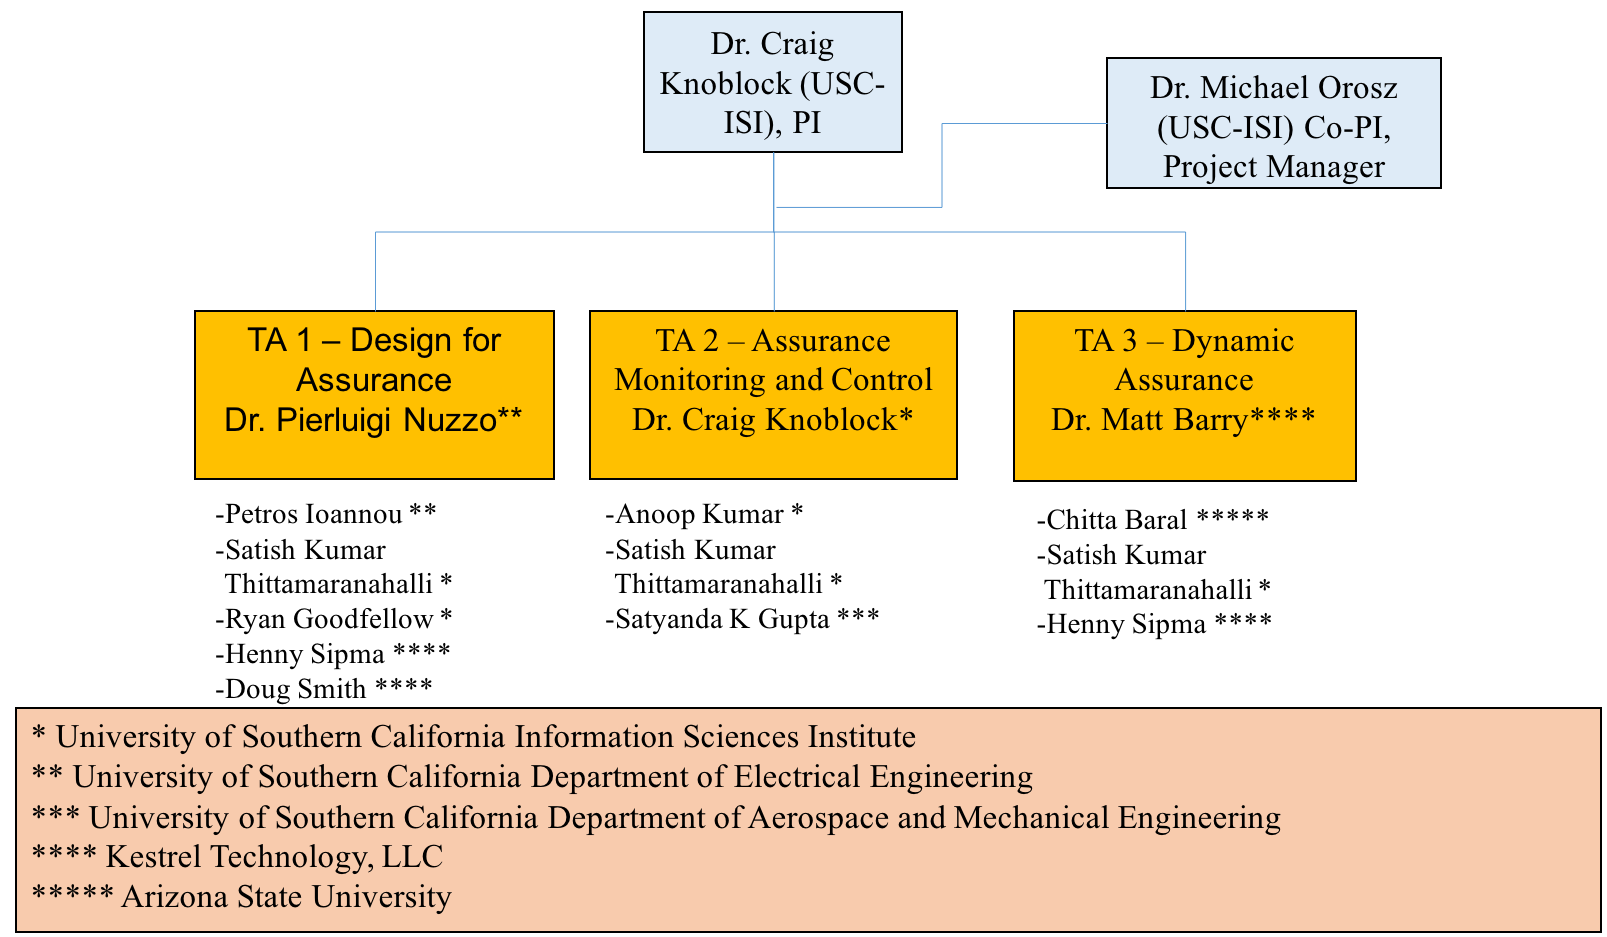
\includegraphics[width=6.0in]{./org-chart2.png}
\caption{\small Organization Chart}
\label{fig:org_chart}
\end{figure}

Coordination: To maximize collaboration and reduce risk to project failure from lack of communication and technical exchange, we plan to employ a wide variety of working styles and communication/coordination so that all can contribute.  At the core of our project will be regularly scheduled meetings bridging the diversely distributed team (Table~\ref{fig:Collaboration_Table}).  These meetings will address project status, identify challenges, implement risk mitigation strategies and participate in technology exchanges and system integration efforts (when appropriate)

\begin{table}[ht]
\caption{\small Project Meetings and Events}
  \centering
  {\footnotesize
\begin{tabular}{|m{3.15in}|m{3in}|} 
\hline
\textbf{Meeting} & \textbf{Frequency} 
\\\hline
Conference calls among investigators (discuss project status, address concerns and project risks) & Weekly
\\
\hline
Technical exchange and coordination meetings using Bluejeans or another videoconference technology & At least twice a month and more frequently as needed
  \\ 
\hline
Face-to-Face meetings (prior to P/I and demonstration meetings) & Every 3 to 6 months and more frequently (especially at the beginning of the project) as needed
 \\\cline{1-2}

\hline
\end{tabular}
}
\label{fig:Collaboration_Table}
\end{table}

\begin{table}[tbhp]
\caption{\small Key Project Team Member Responsibilities}
  \centering
  {\footnotesize
\begin{tabular}{| m{.75in} | m{3.9in}| m{1.5in}|} 
\hline
\textbf{Key Member} & \textbf{Responsibilities} & \textbf{Tasks} 
\\\hline
Dr.\ Craig Knoblock  & Principal Investigator responsible for project, leads TA 2 – Assurance Monitoring and Control.  Will lead the overall project and lead the TA2 team.  Served as the PI on many DARPA projects and has sucessfully led many large teams.    Effort on project:  25\% &
1.1.6, 1.2.2 1.2.3, 1.2.4, 1.3.4, 1.4.1, 
2.1.6, 2.2.2 2.2.3, 2.2.4, 2.3.4, 2.4.1, 
3.1.6, 3.2.2, 3.2.3, 3.2.4, 3.3.4, 3.4.1
\\
\hline
Dr.\ Michael Orosz & Co-Principal Investigator responsible managing the day-to-day operations of the project, assist technical teams as needed, coordinate with TA4 teams.    Has led many large complex multi-disciplined/multi-organizational projects in academic and industry environments.  Effort on project: 50\%
& 1.1.6, 2.1.6, 3.1.6, 1.4.1, 2.4.1, 3.4.1
  \\ 
\hline
Dr.\ Pierluigi Nuzzo 
& 
Co-Principal Investigator.  Leads the TA 1 - Design for Assurance team and conducts research on the formal methods for the design of the TA1 system.  Research experience on methodologies and tools for the design of cyber-physical systems; contracts, interfaces, and compositional methods for embedded system design; the application of automated formal methods and optimization theory to problems in embedded and cyber-physical systems.  Effort on project: 2 months/year (16.6\%)
& 
1.1.1, 2.1.1, 3.1.1 \\
\hline
Dr.\ Matthew Barry
& 
Key personnel.  Leads the TA 3 – Dynamic Assurance.   He will conduct the research on the dynamic assurance case language editors and parsers, the run-time system, and system integrations. Effort on project:  66\%
& 
1.3.2, 2.3.2, 3.3.2\\
\hline
Dr.\ Chitta Baral
& 
Key personnel responsible for learning assurance rules, supporting assurance rules with uncertainty and improving solver speed.  Expertise on ASP solvers, which will be used to reason about the assurance cases. Effort on project: 20\%
& 
1.3.1, 2.3.1, 3.3.1 \\
\hline
Dr.\ Doug Smith 
& 
Key personnel will support formal methods aspects of TA1, and lead the effort on abstract refinement. Expertise in field of automated correct-by-construction program generation.    Effort on project: 40\%
& 
1.1.5, 2.1.5, 3.1.5 \\
\hline
Dr.\ Henny Sipma
& 
Key personnel who will support the program verification tasks under TA1.  Will lead the effort on program verification.   Effort on project:  45\%
& 
1.1.5, 2.1.5, 3.1.5, 1.3.2, 2.3.2, 3.3.2 \\
\hline
Dr.\ Petros Ioannou
& 
Key personnel responsible providing and extending the assurance test bed, which will be available at the start of the project for autonomous vehicles.   Effort on project: 1 month/year (8.3\%)
& 
1.1.2, 2.1.2 (optional), 3.1.2 (optional)
\\
\hline
Dr.\ Satyandra Kumar Gupta
& 
Key Personnel providing autonomous command and control expertise to the TA-2 team.   Will lead the research on safety aware learning on TA2.   Past research on physics-aware decision making to facilitate automation.  Effort on project: 1 month/year (8.3\%)
& 
1.2.1, 2.2.1, 3.2.1 \\
\hline
Dr.\ Anoop Kumar 
& 
Key personnel providing support to the TA 2 project team.  Will lead the research on monitoring \& control and detecting distribution shifts.  Effort on project: 50\%
& 
1.2.1, 1.2.2, 1.2.3, 1.2.4, 2.2.1, 2.2.2, 2.2.3, 2.2.4, 3.2.1, 3.2.2, 3.2.3, 3.2.4\\
\hline
Dr.\ Satish Thittamaranahalli
& 
Key personnel developing scalable algorithms for TA1, TA2, and TA3 project teams.  Has extensive experience on scalable algorithm design, machine learning, and constraint reasoning.  Effort on project: 50\%
& 
1.2.1, 1.2.2, 1.2.3, 1.2.4, 2.2.1, 2.2.2, 2.2.3, 2.2.4, 3.2.1, 3.2.2, 3.2.3, 3.2.4, 1.1.4, 2.1.4, 3.1.4 \\
\hline
Dr.\ Ryan Goodfellow
& 
Key personnel providing support to the TA-1 project. Will lead the research on simulation-based testing.  Has extensive experience on simulation-based testing.  Effort on project:  30\%
& 
1.1.3, 2.1.3, 3.1.3 \\

\cline{1-2}

\hline
\end{tabular}
}
\label{fig:Table_Mgmt}
\end{table}



\newpage
\section{Personnel, Qualifications and Commitment}

{\bf Dr.\ Craig Knoblock}, the PI on this effort, is a Research Professor of both Computer Science and Spatial Sciences at the University of Southern California (USC) and Director of the Intelligent Systems Division at the USC Information Sciences Institute.   He received his Ph.D. from Carnegie Mellon University in computer science. 
%His research focuses on techniques for describing, acquiring, and exploiting the semantics of data.  
In previous projects he has worked on developing  scalable approaches to execution monitoring, accurate detection of sensor failures, and   automatic modeling and reconstruction of sensors.  He has published more than 300 journal articles, book chapters, and conference papers on these topics.  Dr. Knoblock is a Fellow of the Association for the Advancement of Artificial Intelligence (AAAI), a Distinguished Scientist of the Association of Computing Machinery (ACM), a Senior Member of IEEE, past President and Trustee of the International Joint Conference on Artificial Intelligence.
%and winner of the 2014 Robert S. Engelmore Award.  

{\bf Dr.\ Michael Orosz}, a Co-PI on this effort, is a Research Associate Professor of Civil and Environmental Engineering at the University of Southern California (USC) and Research Director of the Decision Systems Group at the USC Information Sciences Institute.  Dr. Orosz has over 30 years’ experience in commercial and government software development, basic and applied research, project management, academic research and has developed and deployed several commercially successful products.  His research interests are in machine learning and decision analytics as applied to intelligence analysis and autonomous command and control such as smart building controls.    Dr. Orosz has extensive experience in managing large complex multi-disciplined/multi-teamed research projects. %funded by DARPA, DHS, DoD, DoE, Industry, NASA, NRO, NSA and ONR.   
He received his Ph.D. in computer science from the University of California, Los Angeles.

{\bf Dr.\ Pierluigi Nuzzo}, a Co-PI on this project, is an Assistant Professor in the Department of Electrical Engineering at the University of Southern California. He received the Ph.D. in Electrical Engineering and Computer Sciences from the University of California at Berkeley. 
%in 2015, and the Laurea degree (MS) in electrical engineering (summa cum laude) from the University of Pisa, Italy, and the Sant'Anna School of Advanced Studies, Pisa, Italy.
%
%He has four years of research experience in analog and mixed signal circuit design as a researcher at IMEC, Leuven, Belgium, and over 10 years experience in design methodologies and tools for mixed-signal integrated circuits and cyber-physical systems, as a researcher at the University of Pisa, IMEC, UC Berkeley, and USC. 
His research interests
include: methodologies and tools for cyber-physical system and mixed-signal
system design; contracts, interfaces and compositional methods for embedded
system design; the application of formal methods and optimization theory to problems in embedded and cyber-physical systems and electronic design automation. 
%
Prof. Nuzzo received %First Place in the operational category and Best Overall
%Submission in the 2006 DAC/ISSCC Design Competition, 
a Marie Curie Fellowship
from the European Union in 2006, 
the University of California at Berkeley EECS
departmental fellowship in 2008, 
%the University of California at Berkeley Outstanding Graduate Student Instructor Award in 2013, 
the IBM Ph.D.
Fellowship in 2012 and 2014, 
%the Best Paper Award from the International Conference on Cyber-Physical Systems (ICCPS) in 2016, 
and the David J.~Sakrison Memorial Prize in 2016 for his doctoral research. 
%He is an author of 1 patent and over 60 publications.

{\bf Dr.\ Satyandra K. Gupta} is Smith International Professor in the Department of Aerospace and Mechanical Engineering at the University of Southern California. %Prior to joining the University of Southern California, he was a Professor in the Department of Mechanical Engineering and the Institute for Systems Research at the University of Maryland. He was the founding director of the Maryland Robotics Center and the Advanced Manufacturing Laboratory at the University of Maryland. 
He served as a program director for the National Robotics Initiative at the National Science Foundation from September 2012 to September 2014.  Dr. Gupta's interest is in the area of physics-aware decision making to facilitate automation. He has published more than 300 technical articles. He is a fellow of the American Society of Mechanical Engineers (ASME) and editor of ASME Journal of Computing and Information Science in Engineering. Dr. Gupta has received the Young Investigator Award from the Office of Naval Research in 2000, CAREER Award from the National Science Foundation in 2001, Presidential Early Career Award for Scientists and Engineers (PECASE) in 2001, Invention of the Year Award at the University of Maryland in 2007, Kos Ishii-Toshiba Award from ASME in 2011, and Excellence in Research Award from ASME in 2013.%, and Distinguished Alumnus Award from Indian Institute of Technology, Roorkee in 2014. %He has also received seven best paper awards at conferences.

{\bf Ryan Goodfellow} is a computer scientist at ISI working in combined cyber physical simulation and emulation platform development. His formal background is in simulation algorithms and modeling techniques using differential-algebraic equations (DAE). He has applied this knowledge in the CPS space by integrating DAE modeling languages and simulation engines with network testbeds to create comprehensive scientific experimentation platforms for cyber-physical systems. These experimentation platforms have been used in the power grid research space. %Ryan is a lead developer on the Deter network testbed, with a strong background in networked and distributed systems engineering. %He is also a combat veteran, serving as a non-commissioned officer and SIGINT team lead for a multi-functional intelligence team in Afghanistan.

{\bf Dr.\ Petros Ioannou} is a Professor in the Department of Electrical Engineering, Director of the Center for Advanced Transportation Technologies and Associate Director for Research for the DOT supported University Transportation Center at USC. He received his MS and PhD from the University of Illinois at Urbana Champaign in Mechanical and Electrical Engineering, respectively. His research interests are in robust adaptive control, vehicle dynamics and control, human factors and safety, automated vehicles, nonlinear systems and Intelligent transportation Systems.  He received the 2016 IEEE Transportation Technologies field award and the 2016 IEEE Control system society Transition to Practice Award. He is a Fellow of IEEE, IFAC and IET and author/coauthor of 8 books and over 400 papers.

{\bf Dr.\ Matthew Barry} will serve as lead for the TA3 tasks. %He will implement the dynamic assurance case language editors and parsers, the run-time system, and system integrations.  He will implement the assurance case arguments and the API for updating argument structure and content.  
Dr. Barry currently is CEO at Kestrel Technology LLC, and previously spent 20 years in NASA space mission operations at the Jet Propulsion Lab and Johnson Space Center.  At NASA Headquarters he led the introduction of dependability case requirements and plans for flight computing systems in upcoming manned space exploration missions, as well as the development of Agency-level software-related safety-critical control system requirements.  He recently served as a Principal Investigator on DHS/Cyber S\&T STAMP (Static Tool Analysis Modernization Program), DARPA CSFV (Crowd Sourced Formal Verification), three NASA Aeronautics R\&D projects, and the AFRL-sponsored Static Analysis of Numerical Algorithms project.  Dr. Barry earned BSME, MS, and PhD degrees in mechanical engineering, and an MBA degree, from Rice University.  

{\bf Dr.\ Henny Sipma} will support the program verification tasks under TA1.  %She is the key person behind the company's {\em KT Advance\/} and {\em KT Transferal\/} static analysis products, and the designer and programmer of the company's core {\em CodeHawk\/} abstract interpretation engine. 
Dr. Sipma currently is the CTO at Kestrel Technology LLC.  She has spent the past 10 years with Kestrel Technology as a static analysis expert; previously developed and taught static analysis techniques as senior research associate at Stanford University for eight years; and developed industrial process controls as an senior systems analyst at Shell.  She has been Principal Investigator or company lead on several recent R\&D projects for Federal agencies, including two projects under the IARPA STONESOUP (Securely Taking On New Executable Software of Uncertain Provenance) program; the DHS Cyber S\&T Gold Standard project; and the DARPA-sponsored STAC (Space-Time Analysis for Cybersecurity) and MUSE (Mining and Understanding Software Enclaves) programs.  Dr. Sipma earned 
%a BS degree in chemistry and an MS degree in chemical engineering at the University of Groningen in The Netherlands, and 
MS and PhD degrees in computer science from Stanford University.  

{\bf Dr.\ Douglas R.\ Smith} will support formal methods aspects of TA1, including the enforcement of safety properties and the generation of monitors.  He is President of Kestrel Technology LLC and Principal Scientist at Kestrel Institute.  He is a Fellow of the American Association of Artificial Intelligence (AAAI) and an ASE Fellow (Automated Software Engineering).  From 1986 to 2000, he taught an advanced graduate course on correct-by-construction software development at Stanford.  
%Dr. Smith has led the development of a series of software synthesis systems, including KIDS (Kestrel Interactive Development System), Specware, Designware, and Planware. 
%Applications domains have included a variety of complex high-performance planners and schedulers for the US Air Force.  He leads current projects on the generation of air mission plans and cyberoperations.  
Other recent projects focused on automated policy enforcement \cite{SmithD0703,SmithD08}, synthesis of secure network protocol codes, and the synthesis of high-performance constraint-solvers\cite{SmithD08c,SmithD13}.  Dr. Smith has over 30 years experience in the field of automated correct-by-construction program generation and has published over 100 papers. He has one patent.  He received the Ph.D. in Computer Science from Duke University% in 1979.  

{\bf Dr. Chitta Baral} is a Professor in the Department of Computer Science and Engineering at Arizona State University. He will support the TA3 efforts on Learning assurance rules, supporting assurance rules with uncertainty and improving solver speed. Dr. Baral has expertise in various aspects of autonomy and Artificial Intelligence. 
He wrote the first book on answer set programming (published by Cambridge University Press) the formal language behind our assurance rules. Some of his other works relevant to this proposal are: goal specification for autonomous systems, automatic construction of control rules for autonomous systems that satisfy given goals, combining machine learning with reasoning in various contexts, including image understanding. %He is the President of KR Inc. He is an associate editor of AIJ and has been an associate editor of JAIR.

{\bf Dr.\ Satish Kumar Thittamaranahalli (T. K. Satish Kumar)} leads the Collaboratory for Algorithmic Techniques and Artificial Intelligence (CATAI) at USC's Information Sciences Institute. He has published over 60 papers on numerous topics in Artificial Intelligence spanning such diverse areas as Constraint Reasoning, Planning and Scheduling, Probabilistic Reasoning, Robotics, Combinatorial Optimization, Approximation and Randomization, Heuristic Search, Model-Based Reasoning, Knowledge Representation and Spatio-Temporal Reasoning. %He %has served on the Program Committees of many international conferences in Artificial Intelligence
He and is a winner of the 2016 Best Robotics Paper Award and the 2005 Best Student Paper Award from the International Conference on Automated Planning and Scheduling. 
Dr. Kumar received his PhD in Computer Science from Stanford University. %In the past, he has also been a Visiting Student at the NASA Ames Research Center, a Postdoctoral Research Scholar at the University of California, Berkeley, a Research Scientist at the Institute for Human and Machine Cognition, a Visiting Assistant Professor at the University of West Florida, and a Senior Research and Development Scientist at Mission Critical Technologies.

\textbf{Dr.\ Anoop Kumar} is a senior computer scientist at USC ISI and has broad expertise in machine learning, statistical modeling, and software engineering.  Dr.\ Kumar is the technical lead on the DARPA RSPACE program and has played a vital role in developing a system that fuses air operations data from multiple sources, maintains world state, and issues warnings. Previously, he led the research and development of the BBN’s election forecasting system for the IARPA OSI program. %Dr.\ Kumar played a significant role in the DARPA DEFT program by developing a model to support integration of output from multiple NLP algorithms. He has contributed at the development to management levels on government research contracts and commercial projects. 
Dr.\ Kumar helped design and develop BBN's commercially available, hosted speech and medical transcription services offering. 

\begin{table}[!tbh]
\begin{footnotesize}
\vspace{-0.1in}

\begin{tabular}{lll}
\begin{tabular}[t]{|l|@{}c@{}|@{}c@{}|@{}c@{}|@{}c@{}|} \hline
Project & Status & \multicolumn{3}{ c| }{Hours} \\ \cline{3-5}
& & P1 & P2 & P3 \\ \hline



\multicolumn{5}{ |c| }{ \textbf{Craig Knoblock} } \\ \cline{1-5}
Safeguard & Pro & 770 & 641 & 641 \\ \cline{1-5}
ELICIT & Cur & 308 & 256 & 120 \\ \cline{1-5}
WTNIC & Cur & 11 & 0 & 0 \\ \cline{1-5}
EFFECT & Cur & 641 & 107 & 0 \\ \cline{1-5}
LinkedMaps & Cur & 203 & 25 & 0 \\ \cline{1-5}
PRINCESS & Cur & 608 & 96 & 0 \\ \cline{1-5}
SCHARP & Cur & 481 & 54 & 0 \\ \cline{1-5}
MINT & Pen & 650 & 534 & 285 \\ \cline{1-5}

\multicolumn{5}{ |c| }{ \textbf{Michael Orosz} } \\ \cline{1-5}
Safeguard & Pro & 1560 & 1300 & 1300  \\ \cline{1-5}
SMC/SY & Cur & 1803 & 0 & 0  \\ \cline{1-5}

\multicolumn{5}{ |c| }{ \textbf{Matthew Barry} } \\ \cline{1-5}
Safeguard & Pro & 2078 & 1690 & 1554 \\ \cline{1-5}
Starlite & Cur & 1840 & 1692 & 0 \\ \cline{1-5}



\multicolumn{5}{ |c| }{ \textbf{Anoop Kumar} } \\ \cline{1-5}
Safeguard & Pro & 1560 & 1300 & 1300 \\ \cline{1-5}

\end{tabular}
&
\begin{tabular}[t]{|l|@{}c@{}|@{}c@{}|@{}c@{}|@{}c@{}|} \hline
Project & Status & \multicolumn{3}{ c| }{Hours} \\ \cline{3-5}
& & P1 & P2 & P3 \\ \hline

\multicolumn{5}{ |c| }{ \textbf{Pierluigi Nuzzo} } \\ \cline{1-5}
Safeguard & Pro & 520 & 433 & 433  \\ \cline{1-5}
Mirage & Cur & 433 & 0 & 0  \\ \cline{1-5}

\multicolumn{5}{ |c| }{ \textbf{Satyandra Gupta} } \\ \cline{1-5}
Safeguard & Pro & 260 & 217 & 217 \\ \cline{1-5}
Human   & Cur & 22 & 0 & 0 \\ \cline{1-5}
Vehicles & Cur & 36 & 0 & 0 \\ \cline{1-5}
Robot & Cur & 116 & 0 & 0 \\ \cline{1-5}
Assembly & Cur & 33 & 0 & 0 \\ \cline{1-5}
Solar & Cur & 4 & 0 & 0 \\ \cline{1-5}

\multicolumn{5}{ |c| }{ \textbf{Petros Ioannou} } \\ \cline{1-5}
Safeguard & Pro & 260 & 217 & 217 \\ \cline{1-5}
CPS & Cur & 130 & 0 & 0 \\ \cline{1-5}

\multicolumn{5}{ |c| }{ \textbf{Ryan Goodfellow} } \\ \cline{1-5}
Safeguard & Pro & 936 & 780 & 780 \\ \cline{1-5}
STEAM & Cur & 416 & 0 & 0 \\ \cline{1-5}


\end{tabular}
&
\begin{tabular}[t]{|l|@{}c@{}|@{}c@{}|@{}c@{}|@{}c@{}|} \hline
Project & Status & \multicolumn{3}{ c| }{Hours} \\ \cline{3-5}
& & P1 & P2 & P3 \\ \hline

\multicolumn{5}{ |c| }{ \textbf{Chitta Baral} } \\ \cline{1-5}
Safeguard & Pro & 659 & 485 & 485 \\ \cline{1-5}
PostdocBP & Cur & 176 & 0 & 0 \\ \cline{1-5}
Languages & Pen & 528 & 264 & 264 \\ \cline{1-5}
CAREER & Pen & 88 & 44 & 44 \\ \cline{1-5}
CHS & Pen & 510 & 255 & 0 \\ \cline{1-5}

\multicolumn{5}{ |c| }{ \textbf{Doug Smith} } \\ \cline{1-5}
Safeguard & Pro & 1222 & 984 & 840 \\ \cline{1-5}
RSPACE & Cur & 342 & 0 & 0 \\ 
\cline{1-5}
PLANX & Cur & 154 & 0 & 0 \\ 
\cline{1-5}
HACCS & Pen & 923 & 769 & 769 \\ 
\cline{1-5}

\multicolumn{5}{ |c| }{ \textbf{Henny Sipma} } \\ \cline{1-5}
Safeguard & Pro & 1372 & 962 & 840 \\ \cline{1-5}
STAC & Cur & 797 & 0 & 0 \\ \cline{1-5}

\multicolumn{5}{ |c| }{ \textbf{Satish Thittamaranahalli} } \\ \cline{1-5}
Safeguard & Pro & 1560 & 1300 & 1300 \\ \cline{1-5}
MapF & Cur & 103 & 103 & 0 \\ \cline{1-5}

\end{tabular}
\end{tabular}

\end{footnotesize}
\caption{Individual commitments of key personnel}
\label{tab:Commitments}
\vspace{-0.2in}
\end{table}

\clearpage
\newpage
\section{Capabilities}


%\subsection{University of Southern California}
USC has strengths in number of areas that are closely related to the proposed work:
\begin{itemize}[itemsep=0pt,leftmargin=*]
\item Dr.\ Nuzzo 
%has over 10-year research experience in embedded system design, from mixed-signal chip design (analog-to-digital converters, frequency synthesizers, software-defined radio), to methodologies and tools for mixed-signal integrated circuits and Cyber-Physical Systems (CPSs), and the application of formal methods and optimization theory to problems in embedded and cyber-physical systems and electronic design automation.  
%His doctoral work 
has done extensive research on contracts and compositional methods for heterogeneous system design and design space exploration, with application to aircraft electric power systems and environmental control systems. His work has helped transition rigorous system design foundations, innovative design methodologies, and new systems engineering paradigms to industry (IBM, United Technologies). 
\item Dr.\ Satyandra K. Gupta has worked on autonomous surface vehicles, autonomous ground vehicles for operation on rugged terrains, and autonomous flapping wing aerial vehicles.   His group has developed a hierarchal decision making approach for realizing autonomous systems. 
%This approach combines task planning and assignment, deliberative trajectory planning, reactive collision avoidance behaviors, and trajectory tracking control layers. 
His group has also developed new methods for learning reactive behaviors in adversarial environments and COLREGS compliant trajectory planning. \item Dr.\ Knoblock has developed methods that learn the relationships between sensors to both identify failures and changes in sensor and reconstruct those sensors, providing estimates of the accuracy of the reconstructed sensors.  
\item Ryan Goodfellow has extensive experience in simulation based testing through high-fidelity CPS testbed environment development and operation, using the Deter network testbed as the core which has supported several large scale government projects from a variety of agencies and thousands of users. %we have developed sophisticated CPS experiments under programs such as NFS RIPS, NIST SmartCities and the DHS Cybersecurity showcase.
\item Dr.\ Ioannou %helped  design and implement adaptive cruise control systems in collaboration with Ford Motor Company, which was commercialized four years before any other company. He 
worked on several DOT funded projects on automated vehicles and intelligent highway systems where he demonstrated his vehicle control designs for safety and performance on actual automated vehicles in test trucks and I-15 highway.
\item Drs.\ Knoblock, Kumar, and Thittamaranahalli have developed highly scalable approaches for monitoring message traffic to identify potential problems and issue warnings and alerts. 
\item Dr. Thittamaranahalli has developed state-of-the-art methods for efficiently solving large-scale search and optimization problems. %These techniques will be applicable in TA2 for safety-aware learning and planning, in TA2 for assurance monitoring and control, and in TA3 for dynamic assessment of assurance cases.

\end{itemize}
%\subsection{Kestrel Technology LLC}

Kestrel Technology's strength is in program analysis, specifically static analysis of both source and binary targets.  The company performs applied R\&D and product development for a variety of static analysis applications  pivoting primarily on the abstract interpretation technique.  The company recently initiated development of program analysis applications using logical equivalence techniques. As a provider of verification evidence in the form of mathematical proofs, the company also has expertise in the design and development of assurance case arguments for high-integrity systems using such evidence. %The company is engaged in a partnership with Wind River Systems to develop program analysis tools for its embedded system developers.  Many of Wind River's customers must develop their products under safety and certification standards, including those using safety cases.  

   

%\subsection{Arizona State University}
Chitta Baral at Arizona State University has developed various software to learn assurance rules and various ASP solvers, which he has made available as open-source.

Most of the software carried forward for implementation or derivation is open source.  The single exception is Kestrel Technology's {\it KT Advance\/} static analysis tool (TA1), in particular the abstract interpretation engine therein, which is company proprietary and is US EAR export-controlled.   
%Owing to mixed funding for the development of that technology 
We will continue to provide the Federal government a restricted use license for that particular item.

There are no specialized facilities, data, or GFE required for this effort. 


\section{Statement of Work}
We propose work for TA 1 – TA 3 for all three phases. All tasks span the four years of the program. For each task we provide an objective, the high-level approach (focusing on the responsibilities of each contributing organization), and the specific approach and milestones planned for each task for each phase. On all tasks, we will deliver design documents, software implementations, demonstrations, and publications. With the exception of several tasks accomplished by Kesler Technology, LLC, all tasks that accomplished at a university (USC/ISI, USC, and ASU) are believed to be fundamental research.   
%\usepackage[table]{xcolor}

{\scriptsize

\begin{longtable} {|p{\textwidth} | }

\hline

\textcolor{blue} {\footnotesize {\textbf{Tasks 1.1.1, 2.1.1, 3.1.1 -Design for Assurance System Models and Formal Verification (USC)}}} \\ \hline
Objective:  Develop contract-based formalisms and mapping tools to represent and reason about LE-CPSs at multiple levels of abstraction and generate assurance cases.  Undertake scalable formal verification and synthesis via Satisfiability Modulo Convex Programming. \\ \hline
Approach:  Develop modeling formalisms to represent components and contracts for LE-CPSs, including physical plant (e.g., autonomous vehicle, sensors, actuators, environment, controllers, and learning components. Formalisms will encompass different control and learning architectures (e.g., neural networks, statistical methods, graphical models, ensemble methods, decision trees) and support mapping between abstractions.   Develop a formal domain-specific language to capture and formalize requirements on LE components, systems, and their dynamics as contracts.   Develop a unifying framework and efficient algorithms to reason about the combination of discrete and continuous dynamics and constraints in the presence of uncertainties in LE cyber-physical systems \\ \hline
Phase 1 (1.1.1):  Milestone 1: Develop initial design followed by development and testing of individual components.  Milestone 2:  Library of components and contracts for the autonomous vehicle application driver.  Milestone 4: Library of components and contracts for the platforms provided by TA4 performers. Extension of the methodology and to support up to 20 continuous dimensions and 2 learning components for the 2 application drivers from TA4.  Milestone 6: -Prototype toolkit (software package) for capturing requirements, for translating them into contracts, for analyzing and validating them using contract operations and relations.  Prototype toolkit for capturing probabilistic requirements and behaviors of LE components, systems, and their dynamics, for translating them into stochastic assume-guarantee contracts, for analyzing and validating them using contract operations and relations, and for synthesizing design and verification artifacts from contracts.  Extension of the SMC framework and toolkit to support reactive and robust task and trajectory planning in the presence of uncertainties. \\ \hline
Phase 2 (2.1.1) Milestone 7: Refinement of design.  Milestone 9: extension of methodology, design, toolkits and libraries to support 40 continuous dimensions, 4 LECs, 30\% monitoring overhead. Extension of the SMC framework and toolkit from Phase 1 to support verification and synthesis on system with 40 dimensions and 4 LECs.  Milestone 10: Demonstration of the SMC framework and toolkit.  Contribution to Phase II report and dissemination of the results in conferences and journals. \\ \hline
Phase 3 (3.1.1) Milestone 11: Update design based on Phase II demo.  Milestones 12-13:  extend methodology, design, toolkits and libraries to support 100 dimensions, 6 LECs and 10\% monitoring overhead.   Milestone 14: Undertake Phase III demonstration on both platforms and submit final project report. \\ \hline
\textcolor{blue} {\footnotesize {\textbf{Tasks 1.1.2, 2.1.2, 3.1.2: Design for Assurance Testbed (USC)} }}\\ \hline
Objective:  Develop a simulation test bed for data generation and LE algorithm testing, redesign and/or refinement.   Simulator used as the test bed until the TA4 platforms are available.   Test bed will be used for internal research/prototype after TA4 platform availability. \\ \hline
Approach:  Leverage previous work on microscopic traffic simulations in urban and rural environments using the commercial software VISSIM and Vortex Studio and built in extensions for automated driving.   Develop testbed for autonomous vehicles in road/off-road environments to allow LEs to collect data, learn and make control decisions on line and in real time by simulating scenarios. The testbed together with analytical tools used to refine and redesign LEs and control algorithms by taking into account effects revealed by the simulation and not accounted for in the design stage.    In the event the TA4 platforms are not available, the test bed will be extended further by integrating all the LE components, controllers and sensors for demonstration purposes and evaluation of the proposed methodology. \\ \hline
Phase 1 (1.1.2):  Milestones 1-2:  Extension of existing simulator test beds.  Milestones 3-5:  Testing of individual components under normal and unpredicatble situations and demonstrating the results in VISSIM under several different driving scenarios. \\ \hline
Phase 2 (2.1.2) – Optional:  Milestones 7-8:  Extension of existing simulator test beds to support the TA1-TA3 teams.  Milestones 9-10:  Support demonstration of technology capable of supporting 40 dimensions, 4 LECs and 30\% monitoring overhead. \\ \hline
Phase 3 (3.1.2) – Optional:  Milestones 11-12:  Extension of existing simulator test beds to support the TA1-TA3 teams.  Milestones 13-14:  Support demonstration of technology capable of supporting 100 dimensions, 6 LECs and 10\% monitoring overhead. \\ \hline
\textcolor{blue} {\footnotesize {\textbf{Tasks 1.1.3, 2.1.3, 3.1.3: Design for Assurance Simulation Based Testing (USC/ISI)}}} \\ \hline
Objective:  Develop external Discrete Control Mechanisms for OpenModelica.  Develop/package virtual-machine based static time dilation systems. Undertake network testbed integration and develop physical system behavioral analysis tooling. \\ \hline
Approach:  Leverage previous external discrete control mechanisms for DAEs, implement similar facilities for OpenModelica to allow LEs to observe and control a physical system over a network. Contributions pushed back upstream to OpenModelica project.  Implement DieCast for modern libvirt.  Develop tooling to deploy integrated CPS models on the Deter network testbed. Apply modern DAE control theory in the form Modelica analysis packages usable by non DAE experts. \\ \hline
Phase 1 (1.1.3):  Milestones 1-2:  Initial CPS simulation concept and components.  Milestones 3-5:  Testing of individual components under normal and unpredictable situations and demonstrating the results capable of meeting 20 dimensions, 2 LECs and 50\% or under monitoring overhead conditions.   Milestone 6: Demonstrate technology in Phase I demonstration, contribute to Phase I final report and disseminate software and publications. \\ \hline
Phase 2 (2.1.3):  Milestones 7-8:  Apply lessons learned from Phase I and extend existing simulations to support 30 dimensions, 3 LECs and 40\% monitoring overhead.  Milestones 9-10:  Support demonstration of technology capable of supporting 40 dimensions, 4 LECs and 30\% monitoring overhead.  Contribute to Phase II final report and disseminate software and publications. \\ \hline
Phase 3 (3.1.3):  Milestones 11-12:  Apply lessons learned from Phase II and extend existing simulations to support 70 dimensions, 5 LECs and 20\% monitoring overhead.  Milestones 13-14:  Support demonstration of technology capable of supporting 100 dimensions, 6 LECs and 10\% monitoring overhead.  Contribute to Phase III final report and disseminate software and publications. \\ \hline
\textcolor{blue} {\footnotesize {\textbf{Tasks 1.1.4, 2.1.4, 3.1.4: Scalable Algorithms for Formal Verification (USC/ISI)}}} \\ \hline
Objective: Develop innovative algorithms for scalable formal verification. \\ \hline
Approach: Use state-of-the-art techniques for solving combinatorial problems with discrete/continuous variables and hybrid constraints. \\ \hline
Phase 1 (Task 1.1.4): Milestones 1-2: Develop initial design plan and initial concepts. Milestones 3-5: Integrate framework that is capable of supporting 20 dimensions, 2 LECs and 0.1x trials to assurance. Milestone 6: Participate in Phase I demonstration, contribute to Phase I final report and disseminate software and publications. \\ \hline
Phase 2 (Task 2.1.4): Milestones 7-8: Apply lessons learned from Phase I and extend existing design to support 30 dimensions, 3 LECs and 0.05x trials to assurance. Milestones 9-10: Demonstrate technology capable of supporting 40 dimensions, 4 LECs and 0.01x trials to assurance. Participate in Phase II demonstration, contribute to Phase II final report and disseminate software and publications. \\ \hline
Phase 3 (Task 3.1.4): Milestones 11-12: Apply lessons learned from Phase II and extend design/approach to support 70 dimensions, 5 LECs and 0.005x trials to assurance. Milestones 13-14: Demonstrate technology capable of supporting 100 dimensions, 6 LECs and 0.001x trials to assurance. Complete integration of technology into TA4 platform. Contribute to Phase III final report and disseminate software and publications. \\ \hline
\textcolor{blue} {\footnotesize {\textbf{Tasks 1.1.5, 2.1.5, 3.1.5: Design for Assurance Program Verification (Kestrel Technology, LLC)}}} \\ \hline
Objective: Develop and integrate program analysis and monitor synthesis functionality with TA1 functions and services and integrate combined TA1 functions with TA4 platform. \\ \hline
Approach: Integrate existing analysis tools into development environment.  Design and implement abstract domains and properties for one or more modeling layers.  Design and implement analyzer front-end for modeling layers.  Implement test framework for verification tools.  Implement content providers and/or consumers for DAC via DAC API.  Leverage existing algorithms and tools to generate monitors for assumptions and unproven safety constraints. Integrate program analysis and monitor synthesis functionality with TA1 functions and services, integrate combined TA1 functions with TA4 platform.   Prepare software and data installation kits and operating instructions;install software and confirm configuration. \\ \hline
Phase 1 (1.1.5) : Milestones 1-2:  Initial framework design and unit tools, TA1-TA3 interfaces defined. Milestones 3-5:  Testing of individual components/tools capable of meeting 20 dimensions, 2 LECs and 50\% or under monitoring overhead conditions.   Milestone 6: Demonstrate technology in Phase I demonstration, contribute to Phase I final report and disseminate software and publications. \\ \hline
Phase 2 (2.1.5): Milestones 7-8:  Apply lessons learned from Phase I and extend existing design to support 30 dimensions, 3 LECs and 40\% monitoring overhead.  Milestones 9-10:  Support demonstration of technology capable of supporting 40 dimensions, 4 LECs and 30\% monitoring overhead.  Contribute to Phase II final report and disseminate software and publications. \\ \hline
Phase 3 (3.1.5): Milestones 11-12:  Apply lessons learned from Phase II and extend existing simulations to support 70 dimensions, 5 LECs and 20\% monitoring overhead.  Milestones 13-14:  Support demonstration of technology capable of supporting 100 dimensions, 6 LECs and 10\% monitoring overhead.  Contribute to Phase III final report and disseminate software and publications. \\ \hline
\textcolor{blue} {\footnotesize {\textbf{Tasks 1.1.6, 2.1.6, 3.1.6: System integration, deployment, and testing (USC/ISI)}}} \\ \hline
Objective: Develop and implement integration, testing and deployment plan supporting TA1 for all three phases. \\ \hline
Approach: Develop an internal TA1 integration and testing plan (unit tests, etc.) and, in close collaboration with TA2 and TA3 performers on project, develop an overall TA1-TA3 integration and testing plan.  Working with TA4 performers, extend and execute plan for TA4 platform (when available). \\ \hline
Phase 1 (1.1.6): Milestones 1-2:  Develop initial integration and testing plan and implement on unit testing.  Milestones 3-5:  Oversee integration and testing of TA1-TA3 components for system capable of supporting 20 dimensions, 2 LECs and 50\% or less monitoring overhead.   Milestone 6: Complete integration of technology into TA4 testbeds, contribute to Phase I final report and disseminate software and publications. \\ \hline
Phase 2 (2.1.6): Milestones 7-8:  Apply lessons learned from Phase I and extend existing integration and testing plan to support 30 dimensions, 3 LECs and 40\% monitoring overhead.  Milestones 9-10:  Support demonstration of technology capable of supporting 40 dimensions, 4 LECs and 30\% monitoring overhead.  Complete integration of technology into TA4 platforms.  Contribute to Phase II final report and disseminate software and publications. \\ \hline
Phase 3 (3.1.6): Milestones 11-12:  Apply lessons learned from Phase II and extend existing integration and testing plan to support 70 dimensions, 5 LECs and 20\% monitoring overhead.  Milestones 13-14:  Support demonstration of technology capable of supporting 100 dimensions, 6 LECs and 10\% monitoring overhead.  Complete integration of technology into TA4 platform.  Contribute to Phase III final report and disseminate software and publications. \\ \hline
\textcolor{blue} {\footnotesize {\textbf{Tasks 1.2.1, 2.2.1, 3.2.1: Safety Aware Learning (USC)} }}\\ \hline
Objective: Enable the system to learn efficiently without violating safety constraints. \\ \hline
Approach: Integrate LECs with search methods to select the optimal actions/maneuvers to maximize mission utility. \\ \hline
Phase 1 (Task 1.2.1): Milestones 1-2:  Develop initial design plan and initial concepts. Milestones 3-5:  Integrate two LECs with search methods and integrate into framework that is capable of supporting 20 dimensions, 2 LECs and 50\% or less monitoring overhead.   Milestone 6: Participate in Phase I demonstration, contribute to Phase I final report and disseminate software and publications. \\ \hline
Phase 2 (Task 2.2.1): Milestones 7-8:  Apply lessons learned from Phase I and extend existing design to support 30 dimensions, 3 LECs and 40\% monitoring overhead.  Milestones 9-10:  Support demonstration of technology capable of supporting 40 dimensions, 4 LECs and 30\% monitoring overhead.  Participate in Phase II demonstration.  Contribute to Phase II final report and disseminate software and publications. \\ \hline
Phase 3 (Task 3.2.1): Milestones 11-12:  Apply lessons learned from Phase II and extend design/approach to support 70 dimensions, 5 LECs and 20\% monitoring overhead.  Milestones 13-14:  Support demonstration of technology capable of supporting 100 dimensions, 6 LECs and 10\% monitoring overhead. Complete integration of technology into TA4 platform.  Contribute to Phase III final report and disseminate software and publications. \\ \hline
\textcolor{blue} {\footnotesize {\textbf{Tasks 1.2.2, 2.2.2, 3.2.2: Assurance Monitor and Guards (USC)}}} \\ \hline
Objective: Build scalable algorithms for assurance monitoring of architectural and safety constraints \\ \hline
Approach: Use physical models to reduce processing of sensor information for assurance monitoring. Use Variable Elimination to handle uncontrollable, Adversarially controlled, or unobservable variables \\ \hline
Phase 1 (Task 1.2.2): Milestones 1-2:  Develop initial design plan and initial concepts.  Milestones 3-5:  Develop monitors for two LECs and integrate into framework that is capable of supporting 20 dimensions, 2 LECs and 50\% or less monitoring overhead.  Develop APIs for integration with TA1 and TA3. Milestone 6: Participate in Phase I demonstration, contribute to Phase I final report and disseminate software and publications. \\ \hline
Phase 2 (Task 2.2.2): Milestones 7-8:  Apply lessons learned from Phase I, incorporate physical models of vehicle-environment interactions and extend existing design to support 30 dimensions, 3 LECs and incorporate physical models to bring down monitoring overhead to 40\% or less.   Milestones 9-10:  Support demonstration of technology capable of supporting 40 dimensions, 4 LECs and 30\% monitoring overhead.  Participate in Phase II demonstration.  Contribute to Phase II final report and disseminate software and publications. \\ \hline
Phase 3 (Task 3.2.2): Milestones 11-12:  Apply lessons learned from Phase II and identify core constraints to monitor and correlation between variables to support 70 dimensions, 5 LECs and 20\% monitoring overhead.  Milestones 13-14:  Support demonstration of technology capable of supporting 100 dimensions, 6 LECs and 10\% monitoring overhead.  Complete integration of technology into TA4 platform.  Contribute to Phase III final report and disseminate software and publications. \\ \hline
\textcolor{blue} {\footnotesize {\textbf{Tasks 1.2.3, 2.2.3, 3.2.3: System integration, deployment, and testing: (USC/ISI)}}} \\ \hline
Objective: Develop and implement integration, testing and deployment plan supporting TA2 for all three phases. \\ \hline
Approach: Develop an internal TA2 integration and testing plan (unit tests, etc.) and, in close collaboration with TA1 and TA3 performers on project, develop an overall TA1-TA3 integration and testing plan.  Working with TA4 performers, extend and execute plan for TA4 platform (when available). \\ \hline
Phase 1 (1.2.3): Milestones 1-2:  Develop initial integration and testing plan and implement on unit testing.  Milestones 3-5:  Oversee integration and testing of TA1-TA3 components for system capable of supporting 20 dimensions, 2 LECs and 50\% or less monitoring overhead.   Milestone 6: Complete integration of technology into TA4 testbeds, contribute to Phase II final report and disseminate software and publications. \\ \hline
Phase 2 (2.2.3): Milestones 7-8:  Apply lessons learned from Phase II and extend existing integration and testing plan to support 30 dimensions, 3 LECs and 40\% monitoring overhead.  Milestones 9-10:  Support demonstration of technology capable of supporting 40 dimensions, 4 LECs and 30\% monitoring overhead.  Complete integration of technology into TA4 platforms.  Contribute to Phase II final report and disseminate software and publications. \\ \hline
Phase 3 (3.2.3): Milestones 11-12:  Apply lessons learned from Phase II and extend existing integration and testing plan to support 70 dimensions, 5 LECs and 20\% monitoring overhead.  Milestones 13-14:  Support demonstration of technology capable of supporting 100 dimensions, 6 LECs and 10\% monitoring overhead.  Complete integration of technology into TA4 platform.  Contribute to Phase III final report and disseminate software and publications. \\ \hline
\textcolor{blue} {\footnotesize {\textbf{Tasks 1.2.4, 2.2.4, 3.2.4: Detecting Distributional Shifts (USC)}}} \\ \hline
Objective:  Develop a comprehensive framework to detect distribution shifts in LECs \\ \hline
Approach: Extend our prior work on sensor failure detection to distribution shifts.  Implement an approach that looks at single variable, sliding window, and distributions and employs classifiers and ensemble methods. \\ \hline
Phase 1 (Task 1.2.4): Milestones 1-2:  Develop initial design plan and initial concepts.  Milestones 3-5:   Develop framework that is capable of supporting 20 dimensions, 2 LECs and 50\% or less monitoring overhead. Extend sensor failure detection in BRASS effort to detect distributional shifts.  Milestone 6: Participate in Phase I demonstration, contribute to Phase I final report and disseminate software and publications. \\ \hline
Phase 2 (Task 2.2.1): Milestones 7-8:  Apply lessons learned from Phase I and  implement sliding window and sampling based methods to support 30 dimensions, 3 LECs and 40\% monitoring overhead.  Milestones 9-10:  Support demonstration of technology capable of supporting 40 dimensions, 4 LECs and 30\% monitoring overhead.  Participate in Phase II demonstration.  Contribute to Phase II final report and disseminate software and publications. \\ \hline
Phase 3 (Task 3.2.1): Milestones 11-12:  Apply lessons learned from Phase II and implement data reduction and machine learning techniques to support 70 dimensions, 5 LECs and 20\% monitoring overhead.  Milestones 13-14:  Support demonstration of technology capable of supporting 100 dimensions, 6 LECs and 10\% monitoring overhead.  Complete integration of technology into TA4 platform.  Contribute to Phase III final report and disseminate software and publications. \\ \hline
\textcolor{blue} {\footnotesize {\textbf{Tasks 1.3.1, 2.3.1, 3.3.1 - Checking Assurance Case Arguments for Dynamic Assurance – (ASU)}} }\\ \hline
Objective: Enhance assurance case DSL to accommodate learning of assurance rules.    Enhance Dynamic Assurance Case (DAC) implementation to support uncertainty.   Enable ASP solver speed improvements 
 \\ \hline
Approach: We will develop algorithms and an implemented module that can learn assurance rules from a set of input-output pairs. We will illustrate the scalability of our method as compared to existing Inductive Logic Programming methods.  We will develop a variant of L that incorporates various uncertainty and automated reasoning related features such as causality, counterfactual reasoning, use of weights for computing probabilities and probabilistic non-monotonicity.  We will develop a highly efficient ASP reasoning system (that forms the heart of our assurance case DSL) by modularizing the ASP programs and making domain specific restrictions (such as stratification on a big part of the program) on the modules \\ \hline
Phase 1 (Task 1.3.1): Milestones 1-2:  Develop initial design plan and initial concepts.  Milestones 3-5:  Integrate two LECs with search methods and integrate into framework that is capable of supporting 20 dimensions, 2 LECs and 50\% or less monitoring overhead.   Milestone 6: Participate in Phase I demonstration, contribute to Phase I final report and disseminate software and publications. \\ \hline
Phase 2 (Task 2.3.1): Milestones 7-8:  Apply lessons learned from Phase I and extend existing design to support 30 dimensions, 3 LECs and 40\% monitoring overhead.  Milestones 9-10:  Support demonstration of technology capable of supporting 40 dimensions, 4 LECs and 30\% monitoring overhead.  Participate in Phase II demonstration.  Contribute to Phase II final report and disseminate software and publications. \\ \hline
Phase 3 (Task 3.3.1): Milestones 11-12:  Apply lessons learned from Phase II and extend design/approach to support 70 dimensions, 5 LECs and 20\% monitoring overhead.  Milestones 13-14:  Support demonstration of technology capable of supporting 100 dimensions, 6 LECs and 10\% monitoring overhead.  Complete integration of technology into TA4 platform.  Contribute to Phase III final report and disseminate software and publications. \\ \hline
\textcolor{blue} {\footnotesize {\textbf{Tasks 1.3.2, 2.3.2, 3.3.2 - Program Verification and Run-Time Monitoring for Dynamic Assurance (Kestrel Technology, LLC)}}} \\ \hline
Objective: Develop the DAC language, the API for DAC interaction between TA1/TA2/TA3 and implement the technology in the three phases \\ \hline
Approach: Develop initial DAC language and APIs and extend based on testing against internal and TA4 provided scenarios. \\ \hline
Phase 1 (Task 1.3.2): Milestone 6: An initial DSL grammar specification; a DAC API Specification, a program client/server protocol and content specification for use interacting with the DAC; initial learning-enabled solver; and integrated DAC API-solver software for the demonstration platform \\ \hline
Phase 2 (Task 2.3.2): Milestone 7:  Updated design/plans based on Phase I lessons learned. Milestone 10: deliver a program client/server protocol and content specification for use interacting with the DAC; initial uncertainty-enabled solver; and integrated DAC API-solver software for the demonstration platform. \\ \hline
Phase 3 (Task 3.3.2): Milestones 11:  Apply lessons learned from Phase II and extend design/plan.  Milestone 14: Deliver a program client/server protocol and content specification for use interacting with the DAC; final and modularity-enabled solver; and integrated DAC API-solver software for the demonstration platform.  \\ \hline
\textcolor{blue} {\footnotesize {\textbf{Tasks 1.3.3, 2.3.3, 3.3.3: Scalable Algorithms for Checking Assurance Arguments (USC/ISI)}}} \\ \hline
Objective: Develop innovative algorithms for efficient dynamic assessment of assurance cases. \\ \hline
Approach: Use state-of-the-art techniques for solving Weighted CSPs to solve ASPs with weights and probabilities. \\ \hline
Phase 1 (Task 1.3.3): Milestones 1-2: Develop initial design plan and initial concepts. Milestones 3-5: Integrate framework that is capable of supporting 20 dimensions, 2 LECs and 10 conditional evidences. Milestone 6: Participate in Phase I demonstration, contribute to Phase I final report and disseminate software and publications. \\ \hline
Phase 2 (Task 2.3.3): Milestones 7-8: Apply lessons learned from Phase I and extend existing design to support 30 dimensions, 3 LECs and 50 conditional evidences. Milestones 9-10: Demonstrate technology capable of supporting 40 dimensions, 4 LECs and 100 conditional evidences. Participate in Phase II demonstration, contribute to Phase II final report and disseminate software and publications. \\ \hline
Phase 3 (Task 3.3.3): Milestones 11-12: Apply lessons learned from Phase II and extend design/approach to support 70 dimensions, 5 LECs and 500 conditional evidences. Milestones 13-14: Demonstrate technology capable of supporting 100 dimensions, 6 LECs and 1000 conditional evidences. Complete integration of technology into TA4 platform. Contribute to Phase III final report and disseminate software and publications. \\ \hline
\textcolor{blue} {\footnotesize {\textbf{Tasks 1.3.4, 2.3.4, 3.3.4 - System integration, deployment, and testing: (USC/ISI)}} }\\ \hline
Objective: Develop and implement integration, testing and deployment plan supporting TA3 for all three phases. \\ \hline
Approach: Develop an internal TA3 integration and testing plan (unit tests, etc.) and, in close collaboration with TA1 and TA2 performers on project, develop an overall TA1-TA3 integration and testing plan.  Working with TA4 performers, extend and execute plan for TA4 platform (when available). \\ \hline
Phase 1 (1.2.3): Milestones 1-2:  Develop initial integration and testing plan and implement on unit testing.  Milestones 3-5:  Oversee integration and testing of TA1-TA3 components for system capable of supporting 20 dimensions, 2 LECs and 50\% or less monitoring overhead.   Milestone 6: Complete integration of technology into TA4 testbeds, contribute to Phase II final report and disseminate software and publications. \\ \hline
Phase 2 (2.2.3): Milestones 7-8:  Apply lessons learned from Phase II and extend existing integration and testing plan to support 30 dimensions, 3 LECs and 40\% monitoring overhead.  Milestones 9-10:  Support demonstration of technology capable of supporting 40 dimensions, 4 LECs and 30\% monitoring overhead.  Complete integration of technology into TA4 platforms.  Contribute to Phase II final report and disseminate software and publications. \\ \hline
Phase 3 (3.2.3): Milestones 11-12:  Apply lessons learned from Phase II and extend existing integration and testing plan to support 70 dimensions, 5 LECs and 20\% monitoring overhead.  Milestones 13-14:  Support demonstration of technology capable of supporting 100 dimensions, 6 LECs and 10\% monitoring overhead.  Complete integration of technology into TA4 platform.  Contribute to Phase III final report and disseminate software and publications. \\ \hline
\textcolor{blue} {\footnotesize {\textbf{Tasks 1.4.1, 2.4.1, 3.4.1 – Project Management: (USC/ISI)}}} \\ \hline
Objective: Provide overall project management for Phase 1.  Assist in system design, integration and testing.  Interface with TA4 performers to ensure collaboration \\ \hline
Approach:  Establish weekly status meetings among team members, collaboration platform (e.g., Dropbox), provide technical assistance to integration efforts, resolve programmatic issues, develop monthly, quarterly and final reports.  Schedule and participate in technical exchange meetings, assist in developing component interfaces, establish test procedures, prototype testing.  Meet with TA4 performers to discuss test scenarios, platform integration and performance issues \\ \hline
Phase 1 (1.2.3): Milestones 1-2:  Establish meeting schedules and collaboration platforms. Assist teams in developing design and undertaking unit testing.  Milestones 3-5: Assist integration and testing of TA1-TA3 components for system capable of supporting 20 dimensions, 2 LECs and 50\% or less monitoring overhead.   Milestone 6: Assist integration of technology into TA4 testbeds, contribute to Phase II final report (C) and disseminate software and publications. \\ \hline
Phase 2 (2.2.3): Milestones 7-8:  Apply lessons learned from Phase II and extend existing integration and testing plan to support 30 dimensions, 3 LECs and 40\% monitoring overhead.  Milestones 9-10:  Support demonstration of technology capable of supporting 40 dimensions, 4 LECs and 30\% monitoring overhead.  Complete integration of technology into TA4 platforms.  Contribute to Phase II final report and disseminate software and publications. \\ \hline
Phase 3 (3.2.3): Milestones 11-12:  Apply lessons learned from Phase II and extend existing integration and testing plan to support 70 dimensions, 5 LECs and 20\% monitoring overhead.  Milestones 13-14:  Support demonstration of technology capable of supporting 100 dimensions, 6 LECs and 10\% monitoring overhead.  Complete integration of technology into TA4 platform.  Contribute to Phase III final report and disseminate software and publications. \\ \hline
 
\end{longtable}
}


% \textcolor{red}{
% Please review the following project schedule outline and either comment or send Craig/Mike comments.   The milestones reflect the need to scale up as the project moves forward.   As communicated below, we plan to have an initial working system by 6 months (the first P/I meeting).  
% }

% Phase I (18 Months):
% \begin{itemize}
% \item 1 Month – Initial Design completed (Milestone 1)
% \item 3 Months – Individual components developed and tested, TA1, TA2 and TA3 Interface Design completed (Milestone 2)
% \item 6 Months (P/I Mtg) – Initial working system for Design Time (i.e., TA1 – TA3 interaction) – includes one LEC (Milestone 3)  [NOTE:  at this time, TA4 teams will be providing scenarios for the demonstration]
% \item 12 Months (P/I Mtg) – Working system for both Design Time and Operation Time (i.e, TA1, TA2 and TA3 interactions), supports 10 dimensions and 1 LEC (Milestone 4)
% \item 17 Months – Working system that supports 20 dimensions and 2 LECs.   Integrate into both TA4 platforms (Milestone 5)
% \item 18 Months (P/I Mtg) – Phase I demonstration on both TA4 platforms (Milestone 6)
% \end {itemize}
% Phase II (15 Months):
% \begin{itemize}
% \item 19 Months – Design review based on Phase I demo (lessons learned)
% \item 25.5 Months (P/I Mtg) – Refined system to support 30 dimensions, 3 LECs, and 40 percent monitoring overhead (Milestone 7)
% \item 32 Months – Working system that supports 40 dimensions, 4 LECs and 30 percent monitoring overhead.  Integrate into both TA4 platforms (Milestone 8)
% \item 33 Months (P/I Mtg) – Phase II demonstration on both TA4 platforms (milestone 9)
% \end {itemize}
% Phase III (15 Months):
% \begin{itemize}
% \item 34 Months – Design review based on Phase II demo (lessons learned)
% \item 40.5 Months (P/I Mtg) – Refined system to support 70 dimensions, 5 LECs and 20 percent monitoring overhead (Milestone 10)
% \item 47 Months – Working system that supports 100 dimensions, 6 LECs and 10 percent monitoring overhead (Milestone 11)
% \item 48 Months (P/I Mtg) – Phase III demonstration on both TA4 platforms (Milestone 12)
% \end {itemize}

% \textcolor{red}{SEE SoW TABLE in GOOGLE DOCS.   Mike has sent invite to team.   
% }
% \vspace{10pt}

% \textcolor{red}{
% For each defined task, please provide the details listed below.  Please include references to the milestones above (e.g., when listing deliverables).   For sub-tasks, please list and describe them.  In addition, please list start/stop dates (in months) based on the outline above.  Mike  will be inserting these sub-tasks into the master schedule that will show up later in this document.
% }
% \textcolor{blue}{
% \begin{itemize}
% \item A general description of the objective.
% \item A detailed description of the approach to be taken to accomplish each defined task/subtask.
% \item Identification of the primary organization responsible for task execution (prime contractor, subcontractor(s), consultant(s)), by name.
% \item A measurable milestone, (e.g., a deliverable, demonstration, or other event/activity that marks task completion).
% \item A definition of all deliverables (e.g., data, reports, software) to be provided to the Government in support of the proposed tasks/subtasks.
% \item Identify any tasks/subtasks (by the prime or subcontractor) that will be accomplished at a university and believed to be fundamental research.
% \end{itemize}
% }
\clearpage
\newpage
\section{Schedule and Milestones}

The schedule is shown in Figure~\ref{fig:sandm} and the milestones are listed in Table~\ref{tab:milestones}.

\begin{table}[ht]
\centering
\caption{The project has the following fourteen (14) milestones}

{\scriptsize
\begin{tabular}{|m{.25in}|m{.25in}|m{4.0in}|m{1.65in}|} 
\hline
Mile-stones & Month & Description & Deliverables \\ \hline
1 & 2 & Initial Design completed.  Design includes finalized research plans, identification of internal TA milestones, initial interfaces between the three TAs, planned interface with the TA4 platforms. &  \\ \hline
2 & 3 & Individual components developed and tested.   TA1, TA2 and TA3 Interface design completed & Quarterly Report \\ \hline
3 & 6 & Initial working system for Design Time (i.e., TA1 – TA3 interaction).  Continued development of TA2.  Supports includes one LEC.   First P/I meeting.   Review TA4 scenarios. & Quarterly Report, slide presentation \\ \hline
4 & 12 & Working system for both Design Time and Operation Time (i.e., TA1, TA2 and TA3 interactions), supports 10 dimensions and one LEC.  Second P/I meeting.   Initial discussions with TA4 teams on interfaces & Quarterly Report, slide presentation \\ \hline
5 & 17 & Working system that supports 20 dimensions and 2 LECs with no more that 50\% monitoring overhead, 10 conditional evidence monitors and 0.1x reduced trails to assurance.   Start integration effort into both TA4 platforms & Working system (software) available for integration into TA4 platforms.  Monthly perfomance and financial reports \\ \hline
6 & 18 & Phase I demonstration on both TA4 platforms & Phase I report, quarterly reports \\ \hline
7 & 19 & Design review based on Phase I demo (lessons learned). &  \\ \hline
8 & 25.5 & Prototype system capable of supporting 30 dimensions, 3 LECs, with no more than 40\% monitoring overhead, 50 conditional evidence and 0.05x reduced trails to assurance.   Third P/I meeting & Quarterly report \\ \hline
9 & 32 & Working system that supports up to 40 dimensions, 4 LECs, with no more than 30\% monitoring overhead, 100 conditional evidence monitors and 0.01x reduced trails to assurance.  Begin Integration into both TA4 platforms & Working system (software) available for integration into TA4 platforms.  Monthly perfomance and financial reports \\ \hline
10 & 33 & Phase II demonstration on both TA4 platforms & Phase II report, quarterly reports \\ \hline
11 & 34 & Design review based on Phase II demo (lessons learned) &  \\ \hline
12 & 40.5 & Refined system to support 70 dimensions, 5 LECs, 500 conditional evidences and 20\% monitoring overhead – Forth P/I meeting & Quarterly report \\ \hline
13 & 47 & Working system that supports 100 dimensions, 6 LECs, 1000 conditional evidences, .001x reduction in assurance trials and 10\% monitoring overhead & Working system (software) available for integration into TA4 platforms.  Monthly perfomance and financial reports \\ \hline
14 & 48 & Phase III demonstration on both TA4 platforms. Phase III report, final project reporet. & Phase III report, quarterly reports, Final project report \\ \hline
\end{tabular}
}
\label{tab:milestones}
\end{table}

\begin{figure}[tbhp]
\begin{center}
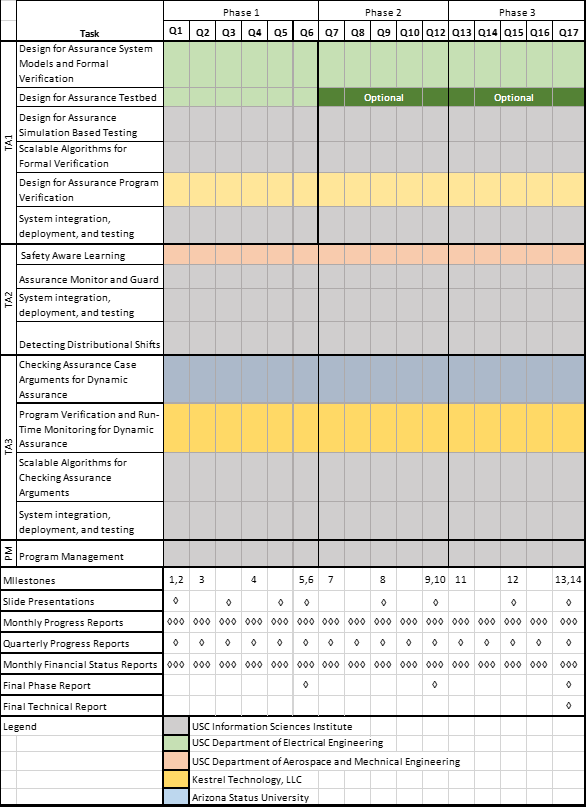
\includegraphics[width=.95\textwidth]{figs/Safeguard_Schedule_V6}
\end{center}
\vspace{-.2in}\caption{Project schedule along with a summary of milestones.  The legend maps task color to organization primary responsible for the task. } 
\label{fig:sandm}
\end{figure}
 

% \section{Level of Effort by Task \textcolor{red}{[Mike/Lisa - 1 pages]}}

% \textcolor{blue}{
% \begin{itemize}
% \item Will be a separate spreadsheet
% \item
% \end{itemize}
% }

\section*{Appendix A: Team Members and Other Information}
\addcontentsline{toc}{section}{Appendix A: Team Members and Other Information}

\baades{This section is mandatory and must include all of the following
components. If a particular subsection is not applicable, state “NONE”.}

\vspace{1ex}

\noindent
\textbf{Team Member Identification}:

\vspace{1ex}

\baades{Provide a list of all team members including the
prime, subcontractor(s), and consultant(s), as applicable. Identify specifically
whether any are a non-US organization or individual, FFRDC and/or Government
entity.}

\begin{centering}

%\small
\begin{tabular}{|p{1.8in}|p{1in}|p{1.1in}|p{0.7in}|p{0.8in}|p{0.7in}|}
\hline
 \textbf{Name} &  \textbf{Role} & \textbf{Organization} & \textbf{Non-US Org?}  & \textbf{Non-US Ind?} &  \textbf{FFRDC or Gov} \\
 \hline
Craig A. Knoblock & Prime & USC & N & N & N\\ \hline
Michael Orosz & Prime & USC & N &  N & N \\ \hline
Satish Thittamaranahalli & Prime & USC & N &  Y & N \\ \hline
Ryan Goodfellow & Prime & USC & N &  N & N \\ \hline
Anoop Kumar & Prime & USC & N & N & N \\ \hline
Satyandra Gupta & Prime & USC & N & N & N \\ \hline
Pierluigi Nuzzo & Prime & USC & N & Y & N \\ \hline
Petros Ioannou & Prime & USC & N & N & N \\ \hline
Chitta Baral & Subcontractor & ASU & N & N & N \\ \hline
Matt Barry & Subcontractor & Kestrel Technology & N & N & N \\ \hline
Douglas Smith & Subcontractor & Kestrel Technology & N & N & N \\ \hline
Henny Sipma & Subcontractor & Kestrel Technology & N & Y & N \\ \hline
\end{tabular} 
\end{centering}

\vspace{1ex}

\noindent
\textbf{Government or FFRDC Team Member Proof of Eligibility to Propose}: NONE

\baades {If
none of the team member organizations (prime or subcontractor) are a
Government entity or FFRDC, state “NONE”.}

\vspace{1ex}

\noindent
\textbf{Government or FFRDC Team Member Statement of Unique Capability}: NONE

\vspace{1ex}

\noindent
\textbf{Organizational Conflict of Interest Affirmations and Disclosure}: NONE

\vspace{1ex}

\noindent
\textbf{Intellectual Property (IP)}: 
\baades {
If no IP restrictions are intended, state “NONE”.
The Government will assume unlimited rights to all IP not explicitly identified as
having less than unlimited rights in the proposal.
For all technical data or computer software that will be furnished to the
Government with other than unlimited rights, provide (per Section VI.B.1) a list
describing all proprietary claims to results, prototypes, deliverables or systems
supporting and/or necessary for the use of the research, results, prototypes
and/or deliverables. Provide documentation proving ownership or possession of
appropriate licensing rights to all patented inventions (or inventions for which a
patent application has been filed) to be used for the proposed project.
}
\begin{centering}

%\small
\begin{tabular}{|p{2.1in}|p{1.2in}|p{1.4in}|p{2in}|}
\hline
\multicolumn{4}{|c|}{COMMERCIAL ITEMS }\\ \hline 
 \textbf{Technical Data, Computer Software To be Furnished With Restrictions} &  \textbf{Basis for Assertion} & \textbf{Asserted Rights Category} & \textbf{Name of Person Asserting Restrictions}  \\  \hline
KT Advance & Developed with mixed funding. & Restricted & David Kulich, Contracts Manager, Kestrel technology, LLC.\\ \hline
\end{tabular} 
\end{centering}

\vspace{1ex}

\noindent
\textbf{Human Subjects Research (HSR)}: NONE

\vspace{1ex}

\noindent
\textbf{Animal Use}: NONE

\vspace{1ex}

\noindent
\textbf{Representations Regarding Unpaid Delinquent Tax Liability or a Felony
Conviction under Any Federal Law}: 
%NONE

\begin{enumerate}
\item
The proposer is  not a corporation that has any unpaid Federal tax liability that has been assessed, for which all judicial and administrative remedies have been exhausted or have lapsed, and that is not being paid in a timely manner pursuant to an agreement with the authority responsible for collecting the tax liability,
\item
The proposer is not a corporation that was convicted of a felony criminal violation under a Federal law within the preceding 24 months.
\end{enumerate}

\vspace{1ex}

\noindent
\textbf{Cost Accounting Standards (CAS) Notices and Certification}:
\baades{
For any proposer who submits a proposal which, if accepted, will result in a CAS-compliant
contract, must include a Disclosure Statement as required by 48 CFR
9903.202. The disclosure forms may be found at
http://www.whitehouse.gov/omb/procurement\_casb
If this section is not applicable, state “NONE”. For further information regarding
this subject, please see www.darpa.mil/work-with-us/additional-baa.
}
NONE


%\section{Appendix B \textcolor{red}{[No Page Count]}}

\section{References}
\bibliographystyle{acm} 
\bibliography{TA3/ta3,TA2/ta2,TA1/ta1}
\end{document}
%%\documentclass[a4paper]{article}
%\documentclass[12pt]{article}
\documentclass[12pt]{dod-blank}

%% Language and font encodings
\usepackage[english]{babel}
\usepackage[utf8x]{inputenc}
\usepackage[T1]{fontenc}

%% Sets page size and margins
%%\usepackage[a4paper,top=3cm,bottom=2cm,left=3cm,right=3cm,marginparwidth=1.75cm]{geometry}
%\usepackage[top=1in, bottom=1in, left=1in, right=1in]{geometry}



%% Useful packages
\usepackage{amsmath}
\usepackage{graphicx}
  \graphicspath{{.}{./image/}}
  \DeclareGraphicsExtensions{.png,.jpg} 
\usepackage[colorinlistoftodos]{todonotes}
\usepackage[colorlinks=true, allcolors=blue]{hyperref}
\usepackage{tabularx}
\usepackage{multirow}
\usepackage{tabulary}
\usepackage{float}
\usepackage{wrapfig}
\usepackage[export]{adjustbox}
\usepackage{comment}
\usepackage{tabularx}
\usepackage{multirow}
\usepackage{tabulary}
\usepackage{enumitem}

\usepackage{listings}
\usepackage{color}
\usepackage{array}
\usepackage{subcaption}
\usepackage{xcolor}




\renewcommand{\textfraction}{0}
\renewcommand{\topfraction}{1.0}
\renewcommand{\bottomfraction}{1.0}

\usepackage{longtable}
%% macros
\newif\iffinal
\finaltrue
\iffinal
  
    \newcommand\baareq[1]{}
    \newcommand\baades[1]{}
 
 
\else
    \definecolor{darkgreen}{rgb}{0,0.4,0}
    \definecolor{darkcyan}{rgb}{0,0.4,0.4}
    \definecolor{darkblue}{rgb}{0,0,0.5}
    
    \newcommand\baareq[1]{{\color{darkcyan}[\textbf{Requirement:} #1]}}
    \newcommand\baades[1]{{\color{darkcyan}[\textbf{Description:} #1]}}
 
\fi




\def\naive{na\"{\i}ve}



\lstset{ 
  backgroundcolor=\color{white},   % choose the background color; you must add \usepackage{color} or \usepackage{xcolor}
  basicstyle=\footnotesize\ttfamily,            % the size of the fonts that are used for the code
  breakatwhitespace=false,         % sets if automatic breaks should only happen at whitespace
  breaklines=true,                 % sets automatic line breaking
  captionpos=b,                    % sets the caption-position to bottom
  commentstyle=\color{mygreen},    % comment style
  % deletekeywords={...},            % if you want to delete keywords from the given language
  escapeinside={\%*}{*)},          % if you want to add LaTeX within your code
  extendedchars=true,              % lets you use non-ASCII characters; for 8-bits encodings only, does not work with UTF-8
  frame=single,	                   % adds a frame around the code
  keepspaces=false,                 % keeps spaces in text, useful for keeping indentation of code (possibly needs columns=flexible)
  keywordstyle=\color{blue}\bfseries\underbar,       % keyword style
  language=Prolog,                 % the language of the code
  % morekeywords={if,and},        % if you want to add more keywords to the set
  numbers=none,                    % where to put the line-numbers; possible values are (none, left, right)
  numbersep=5pt,                   % how far the line-numbers are from the code
  numberstyle=\tiny\color{mygray}, % the style that is used for the line-numbers
  rulecolor=\color{black},         % if not set, the frame-color may be changed on line-breaks within not-black text
  showspaces=false,                % show spaces everywhere adding particular underscores; it overrides 'showstringspaces'
  showstringspaces=false,          % underline spaces within strings only
  showtabs=false,                  % show tabs within strings adding particular underscores
  stepnumber=2,                    % the step between two line-numbers. If it's 1, each line will be numbered
  stringstyle=\color{mymauve},     % string literal style
  tabsize=2,	                   % sets default tabsize to 2 spaces
  title=\lstname                   % show the filename of files included with \lstinputlisting; also try caption instead of title
}

% apply trick for additional keywords for our AC DSL
\lstset{
	emph={for, if, and, or},
    emphstyle={\color{blue}\bfseries\underbar}
}




\title{DARPA Assured Autonomy}
\author{Technical Volume- \textcolor{red}{Thirty-Eight (38) pages max}}

\begin{document}
\pagenumbering{roman}
 
\begin{center}
\large{\textbf{Volume 1: Technical and Management Proposal}}
\end{center}
\textbf{BAA Number:} DARPA-HR001117S0045 \\
\textbf{Technical Area:} TA1, TA2, and TA3 \\
\textbf{Proposal Title:} Assured Autonomy for Learning Enabled Vehicles (Safeguard) \\
\textbf{Lead Institution:} University of Southern California \\
\textbf{Type of organization: } “OTHER EDUCATIONAL” \\

\begin{tabularx}{\linewidth}{XX}

 \textbf{Technical Point of Contact} &  \textbf{Administrative Point of Contact }   \\
Dr.\ Craig A. Knoblock  & Sapphire Masterson  \\ 
USC Information Sciences Institute & USC Dept. of Contracts \& Grants \\
4676 Admiralty Way, Suite 1001 & 4676 Admiralty Way, Suite 1001 \\
Marina del Rey, CA 90292 & Marina del Rey, CA 90292 \\
Tel: 310-448-8786 &  Tel: (310) 448-9161 \\
E-mail: knoblock@isi.edu  & E-mail: sapphirm@usc.edu \\
\end{tabularx}
\\
\\
\textbf{Award instrument requested:}  Procurement Contract, Cost-Reimbursement, No Fee
\\
\\
\textbf{Total amount of the proposed effort:} \$ ...\\
Phase I: \$ ... \\
Phase II: \$ ... \\
Phase III: \$ ... \\
\\
\textbf{Place(s) of performance:} USC, Marina del Rey, CA; Los Angeles, CA;  Tempe, AZ; Palo Alto, CA \\
\textbf{Period(s) of performance:} 04/02/2018 - 03/31/2022     \\
\\
\textbf{Other team members:} \\
\begin{tabularx}{\linewidth}{XX}
Kestrel Technology  & Arizona State University \\
(small business) & (Other Educational)\\
POC: Matthew Barry & POC: Chitta Baral\\
3260 Hillview Avenue & Department of Computer Science and Engr. \\
Palo Alto, CA 94304 & Ira A. Fulton School of Engineering \\ 
phone: (832)205-4876 & Arizona State University\\ 
mrbarry@kestreltechnology.com & Brickyard Suite 572, 699 S. Mill Avenue \\
& Tempe, AZ 85281-8809, U.S.A.\\
& email: chitta@asu.edu\\
\end{tabularx}
\\
\textbf{Proposal validity period: } 180 days\\
\\
\textbf{Data Universal Numbering System (DUNS) number: } 072933393\\
\textbf{Taxpayer identification number:} 95-1642394\\
\textbf{Commercial and Government Entity (CAGE) code:} 1B729 Marina del Rey, CA\\
\textbf{Proposer’s reference number (if any):}  4409-0\\

\newpage
\section{Table of Contents}
\tableofcontents

\newpage
\pagenumbering{arabic}
\section{Executive Summary}
As we rapidly move into a world where machine learning plays a central role in realizing autonomous systems, it is becoming increasingly important to develop techniques that assure that these systems will operate safely and perform as expected. Current approaches are limited to providing assurance for systems with limited or no  learning capabilities. In this context, DARPA's Assured Autonomy BAA seeks to \emph{develop rigorous design and analysis technologies for continual assurance of learning-enabled autonomous systems}. USC in collaboration with Kestrel Technology and ASU is pleased to submit a comprehensive TA1, TA2, and TA3 proposal entitled \emph{``Assured Autonomy for Learning Enabled Vehicles (Safeguard).''} We plan to provide an end-to-end solution to support autonomous systems with learning-enabled components, ranging from design technologies for assurance, to assurance monitoring and control techniques, to representation and online evaluation of assurance cases. We have assembled a strong team of experts that cover the range of technologies that are required to create such an end-to-end system. If successful, the project will provide the technologies for building the next-generation of learning-enabled autonomous systems.  The entire project will take four years and cost \textcolor{red}{\$??}, with an initial version completed at the end of Phase I and successive versions with additional capabilities and improved scalability at the end of Phase II and Phase III.  

In the remainder of this section, we first introduce an  unmanned surface vehicle scenario that will be used throughout the proposal to describe the approach.  Next, we describe our approach to design, monitoring, and dynamic assurance. Finally, we introduce the team involved in the project. 

\textbf{Motivating Scenario.} Consider an autonomous unmanned surface vehicle (USV) guarding a valuable asset in the ocean when an unknown vehicle  approaches the security perimeter, under challenging weather conditions. In this scenario, the USV is required to approach the intruding vehicle, issue a warning signal, and escort it to a safe distance from the controlled area. However, as the USV has no a priori knowledge of its external environment behaviors (e.g., water depth, waves, wind, current, visibility), pre-computing a feasible trajectory, let alone optimal, becomes a non-trivial problem. For trajectory planning, the USV must continuously perform the following tasks:
\begin{itemize}[itemsep=0pt,leftmargin=*]
 \item Sense the current state of the surrounding environment (e.g., water depth, waves, wind, current, visibility) and estimate its own maneuverability constraints (e.g., braking distance, available acceleration, maximum velocity, turning radius, turning rate, safety distance) based on the state of the environment;      
\item Sense the static obstacles in the sensor range and generate a traversability map;
\item Sense the moving obstacles and classify them;   
\item Predict future trajectories of moving obstacles; 
\item Determine if any of the COLREGS \cite{commandant1999international} rules will be in effect with respect to one or more of the nearby vessels and identify the vessels with the right of way.    
\end{itemize}
The above information will be used by the trajectory planner to compute an initial trajectory, which will be continuously refined as the USV gathers additional information.
% It is not possible for the USV to be tested in every possible environment. 
The USV will use learning enabled components to take  decisions as it encounters new situations, such as  
\begin{itemize}[itemsep=0pt,leftmargin=*]
\item Classifiers to identify moving obstacles based on physical appearance and motion signatures,
\item Algorithms to estimate the sensor capabilities in adverse weather conditions,   
\item Algorithms to accurately estimate uncertainty in the environment, 
\item Classifiers to generate traversability maps,
\item Prediction of external vessel behaviors based on motion histories, 
\item Reinforcement learning  to ensure COLREGS compliance of maneuvers,  
\item Algorithms to learning pursuit behaviors.  
\end{itemize}
Learning enabled components will interact with each other in complex ways, where a misclassification error in one component may eventually compromise the entire mission.   
% We will need to make sure that each learning enabled components has a run-time monitor that will ensure that the assumptions made by the learning-enabled component remain valid and prevent erroneous learning. 
% For example, if the vehicle is exhibiting significant error in trajectory tracking, then simply downgrading the trajectory tracking error value may not be a good option.  The failure of prediction of trajectory tracking error might be due to the presence of a significant wake caused by a nearby vessel. The presence of the nearby vessel can be used to explain the degradation in trajectory tracking performance. As the vessel moves away, we can expect the trajectory tracking performance to return to the predicted level.  
While exhaustive validation of learning-enabled cyber-physical systems (LE-CPSs) is a prohibitive task~\cite{Kalra16},
their complexity, heterogeneity, and highly dynamic nature
make it challenging to even leverage existing model-based development techniques to effectively assess system correctness 
% dependability, 
at design time or enforce it at runtime.

\textbf{Design for Assurance.} Safeguard uses a platform-based design approach~\cite{Nuzzo15b} to organize the design process for a LE-CPS and to build assurance cases. Composite models are developed at several levels of abstraction,
from top-level system requirements and safety constraints down to the
implementation level.  Intermediate levels add detail to the levels
above.  The different levels are connected by refinement mappings that
allow properties established at one level to be preserved at the next
level (see Figures~\ref{fig:methodology} and~\ref{fig:assurance}).

Contracts are used to formally specify components and composite models
in terms of (1) Assumptions -- the assumed behaviors of the
environment and the behaviors of other components, and (2) Guarantees
-- the behavior properties that a model guarantees if it operates in a
context that satisfies its assumptions.  A calculus of contracts
allows horizontal composition of contracts to generate contracts for
composite models.  Vertical contracts are used to specify the mapping
or refinement relation between models at different levels of
abstraction.  The system design process starts with a high-level
contract that expresses overall system assumptions and requirements.
Subsequent levels express models with increasing detail until the
lowest level expresses the system in terms of hardware components and
their software controllers.

The assurance case for a CPS arises from the horizontal and vertical
structure of the design in several ways.  The components used within a
particular level are either (1) synthesized using
correct-by-construction design tools together with proofs, (2) derived
statically or dynamically using safety-aware machine-learning
techniques, (3) written manually and verified by analysis tools, or
(4) written manually and validated by extensive testing.  The
assurance case for the whole reflects its compositional structure.  We
anticipate that well-specified contracts together with the calculus of
contracts will eliminate well-known problems with unexpected emergent
behaviors in CPS systems.

The assurance case for the lowest-layer design arises from both the
intra-level assurance and from properties and their proofs that are
preserved under the refinement mapping from the top-level
requirements.  The refinement mappings between model layers will be
constructed using a variety of techniques.  A contract at an abstract
level can be mapped to a component or refined contract by (1)
retrieval of pre-verified components from a platform library, (2)
synthesis using correct-by-construction design and optimization tools,
or (3) manual coding to satisfy a contract.  The mapping of a
composite model will be composed from the mappings of its constituent
components or contracts.  When a composite model cannot be mapped
compositionally to the next level, it will be generated using
correct-by-construction design and optimization tools.

\textbf{Assurance Monitoring and Control.}
We provide an integrated framework for safety-aware learning, assurance monitoring and control, detecting distribution shifts. Three major components offer an efficient TA2 architecture as well as interfaces with TA1 and TA3, that is, (a) safety-aware learning and planning, (b) assurance monitors for guarding architectural and safety constraints; and (c) distribution shift detection.

We will develop a new learning-enabled online decision-making framework that allows opportunistically composing a sequence of actions (maneuvers) to reduce uncertainty in the system capability model without suspending the progress toward the mission goals or compromising safety. Each candidate action is evaluated based on three criteria: (1) the risk of violating a safety constraint using the current uncertainties in the parameter estimates; (2) its relevance to the mission goals; (3)  its expected information gain, i.e., reduction in uncertainty, with respect to the parameter estimates. These evaluations are combined to produce a cumulative mission utility value for each action that drives our learning-enabled decision-making framework. The problem of generating and evaluating sequences of actions can be posed in several way. For example, it can be solved using a branch-and-bound search method like Anytime A*, or formulated with the finite-horizon Markov Decision Process (MDP) framework. We will develop new scalable search strategies to solve this problem efficiently, by potentially evaluating a recent method developed at USC, called FastMap, that can significantly improve the execution time. 

We will develop monitors for architectural and safety constraints. 
% While these constraints can be checked over and over again as sensor information flow in, this naive strategy accounts for a lot of computational overhead. 
To achieve scalability and decrease the overhead, we propose the application of a technique that we currently use in DARPA's RSPACE program, which leverages a physical model of the vehicles dynamics and its interactions with the environment to efficiently determine the readout frequency. We propose two  extensions of this basic idea. First, we will use the theory of Variable Elimination to prioritize which variables to monitor, e.g., controllable, versus uncontrollable, adversarially controlled, or unobservable variables. Second, we invoke the dynamic assessment of assurance cases only when needed. This  decreases the number of times dynamic assessment of assurance cases is initiated as well as the communication bandwidth between the TA2 and TA3 components.

Finally, we will identify a distribution shift by combining statistical and machine learning techniques to differentiate between environmental and sensor changes. We will exploit a categorization of the shifts based on their cause and duration as well as extend our earlier work on detecting and mitigating sensor failures for all types of monitored variables.  

\textbf{Dynamic Assurance:} The Safeguard {\em design for assurance\/} activity takes a systems-theoretic stance toward safety.  Consequently, it presumes that safety is an emergent property of the system, and that hazards can present themselves through unintended interactions and performance violations in addition to causal events such as component failures.  Our design approach includes consideration of intent as well as hazard analysis and mitigation.  The artifacts from these activities populate contracts and assumptions for the dynamic assurance case.  
We thus build safety into the product by working at a systems-level viewpoint, using lexicon and design patterns familiar to both hardware and software engineers; safety is an emergent property of the system, not an afterthought.  
As system behavior evolves during runtime owing to learning, threats, degradation, or some other factor, the dynamic assurance case identifies whether the safety constraints continue to be satisfied.  If not, it provides notifications or issues recovery instructions directly from a lookup table.

Our implementation of the dynamic assurance case employs a declarative knowledge base inference engine and a domain-specific language tailored to our approach.  We have used them successfully for assurance case tool sets and arguments, and will extend them to reason about uncertainty and learning.  Our approach to achieve scalability is to specialize solvers toward modularity and to take advantage of domain knowledge.  Specifically, we will develop answer set programming techniques for context-dependent learning for reasoning about the learning-enabled components as well as learning assurance rules.  We will develop new formalisms for uncertainty to include causality, using weights for computing probabilities, and probabilistic non-monotonicity.  To achieve scaling objectives we will implement specializations using modularity, weighted CSPs, and message passing. 

% The system safety constraints revealed from that design become the key elements of our dynamic assurance case.  Our verification tools ensure the constraints are relevant, identifiable, and their implementation and effect observable.  

\textbf{Team.} We have assembled a team that is exceptionally well-qualified to build the proposed Safeguard system.  The team will be led by Dr.\ Craig Knoblock, the Principal Investigator for the effort, who currently leads the Intelligent Systems Division at the Information Sciences Institute.  He has led many large DARPA and IARPA projects over the years and has a strong track record in conducting leading edge research and then transitioning the technology to commercial use.  He will be supported by Dr.\ Michael Orosz as the Project Manager, who also has  experience in managing large research projects and on autonomous systems.  The TA1 team will be led by Dr.\ Pierluigi Nuzzo, who is an expert in embedded system design methodologies and the  application of formal methods to cyber-physical systems.  The TA1 team also includes Dr.\ Doug Smith, who has spent many years working on scalable correct-by-construction techniques and Dr.\ Henny Sipma, who has significant experience in applying program verification methods to real-world problems.  The TA1 team also includes Ryan Goodfellow, who has done a large amount of work on simulation-based testing.  The TA2 team will be led by Dr.\ Knoblock who has worked on topics related to both monitoring and detecting distribution changes.  He will be supported by Dr.\ Satyandra Gupta, who is an expert on autonomous surface vehicles as well as on safety-aware learning. He will also be supported by Drs.\ Anoop Kumar and Satish Thittamaranahalli, who have also previously worked on efficient methods for execution monitoring.  The TA3 team will be lead by Dr.\ Matthew Barry, who has experience in creating the technologies for assurance cases.  He will be supported by Dr.\ Chitta Baral, who is an expert on ASP solvers and by Dr.\ Thittamaranahalli who is an expert on SAT solvers, both of which will be applied to provide scalable assurance case reasoning.  Finally, Dr.\ Petros Ioannou, who is an expert on control systems for autonomous vehicles will provide an autonomous vehicle platform, which will form the focus of our work until the TA4 teams provide additional vehicle platforms for development.  

\newpage
\section{Innovative Claims and Deliverables}

In this project we will develop and build an end-to-end system for assured autonomy.  This section describes the key innovations by technical area and then the overall deliverables of the project.

\paragraph{Design for Assurance}

\begin{itemize}[itemsep=0pt,leftmargin=*]
\item We address the LE-CPS design challenges via a holistic approach that can contextually generate design artifacts and assurance cases. We develop a compositional, contract-based modeling framework, methods, and tools to support the design process from system-level requirement capture,  formalization, and analysis, to the generation, testing, and continual monitoring of software and hardware artifacts in feedback loop with a physical process.

\item We develop compositional abstractions and interfaces (vertical contracts) that can  bridge heterogeneous formalisms and heterogeneous decomposition architectures to make system analysis and synthesis tractable, consistently combine different verification and synthesis methods at design time, and provide seamless support for dynamic assurance at run time. %We aim to quantitatively capture the confidence in the satisfaction of requirements under uncertain or unknown conditions, and resilience properties of  systems at different abstraction levels, to enable trade-off evaluation between resilience, performance, and cost.

\item We develop a unifying framework and efficient algorithms to reason about the combination of discrete and continuous dynamics and constraints in the presence of uncertainties in LE-CPS using a satisfiability modulo convex approach~\cite{Shoukry2017} for contract-based system verification and scalable trajectory planning.  

\item We provide an environment for high-fidelity CPS testing, in which production-ready software, e.g.,  safety-critical learning and control, may be deployed and tested 
% by extending the Cypress testbed environment \cite{Goodfellow2015Cypress:Systems} 
with time dilation facilities, so that it synchronizes with a physical simulation that is not necessarily running in real time, while still having the perception of real time.

\item We 
% These facilities allow a cyber system to be  
propose an approach for unanticipated behavior space identification and test coverage maximization which leverages results from the theory of differential algebraic equation (DAE)~\cite{Berger2013ControllabilitySurvey,Ilchmann2005ATheory,BergerOnSystems,Lamour2013} 
to prune the behavior search space and identify smaller regions of interest for efficient simulation-based testing. 
% We then compute the intersection of these two behavior spaces and restrict our simulation based testing search space to this subspace.
\end{itemize}

\paragraph{Assurance Monitoring and Control}

\begin{itemize}[itemsep=0pt,leftmargin=*]
\item 
%We integrate safety-aware learning into the overall decision making problem. The goal is to maximize mission utility without violating the safety constraints. 
Our safety-aware learning framework enables the system to opportunistically select and execute actions to assist the learning-enabled component in reducing model uncertainty without compromising safety or deviating from the mission goals. The value of uncertainty reduction is explicitly incorporated in the optimization process for selecting the best action.  
\item For safety-aware learning, we propose the idea of preprocessing the search space of the problem domain before queries and observations come in. With such a linear-time preprocessing phase, the performance of search and optimization algorithms can be significantly boosted. For example, in regular A* search, the intensional or extensional search space can be preprocessed in near-linear time to yield an embedding of each state as a point in Euclidean space~\cite{cujakk}. Then, when the query comes in, A* search can make use of these Euclidean distances as heuristic distances between two states to yield order-of-magnitude speedups. 
%In Anytime A* for safety-aware learning and planning, this leads to a significantly better quality of actions chosen within a time limit, and in the MDP framework, the same ideas can be used to improve the convergence of Bellman updates for safety-aware Reinforcement Learning.
\item As massive amounts of sensor information flow in, it is imperative for us to efficiently process this information for monitoring architectural and safety constraints. Building on our past work on similar tasks, we propose novel technologies for efficiently monitoring constraints. These algorithms can yield an exponential reduction in the amount of sensor data that needs to be processed. Doing this also reduces the message complexities between the various modules. %We also propose to use the theory of Variable Elimination (VE) to monitor constraints with uncontrollable, adversarially controlled, and/or unobservable variables. VE yields a substrate constraint to monitor that characterizes a dominant strategy of the controllable variables over the uncontrollable, adversarially controlled, and/or unobservable variables.
\item We will develop techniques to identify  distributional shifts and determine the underlying cause (e.g., change in environment, sensor failure,   etc.), as well as strategies for handling the various distributional shifts.   Notably, we propose to build on our past work and use compact representations to exploit historical data to identify distributional shifts.
\end{itemize}

\paragraph{Dynamic Assurance}

\begin{itemize}[itemsep=0pt,leftmargin=*]

\item We demonstrate the integration of dynamic assurance for safety-critical learning-enabled dynamic systems in which evolutionary behaviors are expected and tolerated as a property of the functionality.   The impact will be consequential contributions safety-critical dynamic systems in which evolutionary behaviors are expected and tolerated as portion of the functionality.   
\item We implement dynamic assurance by combining features of system safety, formal methods, logic programming, uncertain reasoning, and domain-specific languages.  We populate assurance case arguments at several levels of modeling and implementation abstraction, using the analysis results to produce design-time evidence supporting assurance claims.  
%We provide automated reasoning about the assurance case itself to produce verification, consistency, and completeness results for the argument.  Dynamic assurance results then yield trusted explanations of whether safety constraints and assumptions and other contracts still hold during the collection of runtime evidence from monitors. 
\item We develop and demonstrate ASP formalisms crucial to applications in dynamic assurance. We demonstrate the suitability of the technology especially for assurance case arguments owing to the improved legibility, consistency and completeness checks, handling of uncertain and default reasoning, and scalability.  
%We will produce modularized solvers for enhanced performance based on recent algorithmic developments in exploiting structure, kernelization, and message passing. We provide a formalism to enable learning of assurance rules. 
We provide a novel approach to handling uncertainty that provides the ability to do causal and counter-factual reasoning as well as probabilistic non-monotonicity.  Overcoming limitations of traditional inductive logic techniques, we develop a novel iterative and incremental approach based on context dependent learning. 
\end{itemize}

\paragraph{Deliverables}
During the course of this project, we will build and deliver a fully-operational system that covers all three of the technical areas.  The detailed capabilities of this system are described in the individual technical sections.  The resulting system will be available as open source under a permissive license, which will allow other organizations to use the work, extend it in new directions, and even commercialize the software.  Kestrel Technology has significant experience in this space and has built and applied these types of technologies to a variety of real world tasks.  Kestrel is ideally suited to pursue commercial uses of this technology and the permissive license will facilitate exploring these opportunities since there will be no need to negotiate intellectual property rights.  

\newpage
\section{Technical Plan}
%%\documentclass[a4paper]{article}
%\documentclass[12pt]{article}
\documentclass[12pt]{dod-blank}

%% Language and font encodings
\usepackage[english]{babel}
\usepackage[utf8x]{inputenc}
\usepackage[T1]{fontenc}

%% Sets page size and margins
%%\usepackage[a4paper,top=3cm,bottom=2cm,left=3cm,right=3cm,marginparwidth=1.75cm]{geometry}
%\usepackage[top=1in, bottom=1in, left=1in, right=1in]{geometry}



%% Useful packages
\usepackage{amsmath}
\usepackage{graphicx}
  \graphicspath{{.}{./image/}}
  \DeclareGraphicsExtensions{.png,.jpg} 
\usepackage[colorinlistoftodos]{todonotes}
\usepackage[colorlinks=true, allcolors=blue]{hyperref}
\usepackage{tabularx}
\usepackage{multirow}
\usepackage{tabulary}
\usepackage{float}
\usepackage{wrapfig}
\usepackage[export]{adjustbox}
\usepackage{comment}
\usepackage{tabularx}
\usepackage{multirow}
\usepackage{tabulary}
\usepackage{enumitem}

\usepackage{listings}
\usepackage{color}
\usepackage{array}
\usepackage{subcaption}
\usepackage{xcolor}




\renewcommand{\textfraction}{0}
\renewcommand{\topfraction}{1.0}
\renewcommand{\bottomfraction}{1.0}

\usepackage{longtable}
%% macros
\newif\iffinal
\finaltrue
\iffinal
  
    \newcommand\baareq[1]{}
    \newcommand\baades[1]{}
 
 
\else
    \definecolor{darkgreen}{rgb}{0,0.4,0}
    \definecolor{darkcyan}{rgb}{0,0.4,0.4}
    \definecolor{darkblue}{rgb}{0,0,0.5}
    
    \newcommand\baareq[1]{{\color{darkcyan}[\textbf{Requirement:} #1]}}
    \newcommand\baades[1]{{\color{darkcyan}[\textbf{Description:} #1]}}
 
\fi




\def\naive{na\"{\i}ve}



\lstset{ 
  backgroundcolor=\color{white},   % choose the background color; you must add \usepackage{color} or \usepackage{xcolor}
  basicstyle=\footnotesize\ttfamily,            % the size of the fonts that are used for the code
  breakatwhitespace=false,         % sets if automatic breaks should only happen at whitespace
  breaklines=true,                 % sets automatic line breaking
  captionpos=b,                    % sets the caption-position to bottom
  commentstyle=\color{mygreen},    % comment style
  % deletekeywords={...},            % if you want to delete keywords from the given language
  escapeinside={\%*}{*)},          % if you want to add LaTeX within your code
  extendedchars=true,              % lets you use non-ASCII characters; for 8-bits encodings only, does not work with UTF-8
  frame=single,	                   % adds a frame around the code
  keepspaces=false,                 % keeps spaces in text, useful for keeping indentation of code (possibly needs columns=flexible)
  keywordstyle=\color{blue}\bfseries\underbar,       % keyword style
  language=Prolog,                 % the language of the code
  % morekeywords={if,and},        % if you want to add more keywords to the set
  numbers=none,                    % where to put the line-numbers; possible values are (none, left, right)
  numbersep=5pt,                   % how far the line-numbers are from the code
  numberstyle=\tiny\color{mygray}, % the style that is used for the line-numbers
  rulecolor=\color{black},         % if not set, the frame-color may be changed on line-breaks within not-black text
  showspaces=false,                % show spaces everywhere adding particular underscores; it overrides 'showstringspaces'
  showstringspaces=false,          % underline spaces within strings only
  showtabs=false,                  % show tabs within strings adding particular underscores
  stepnumber=2,                    % the step between two line-numbers. If it's 1, each line will be numbered
  stringstyle=\color{mymauve},     % string literal style
  tabsize=2,	                   % sets default tabsize to 2 spaces
  title=\lstname                   % show the filename of files included with \lstinputlisting; also try caption instead of title
}

% apply trick for additional keywords for our AC DSL
\lstset{
	emph={for, if, and, or},
    emphstyle={\color{blue}\bfseries\underbar}
}




\title{DARPA Assured Autonomy}
\author{Technical Volume- \textcolor{red}{Thirty-Eight (38) pages max}}

\begin{document}
\pagenumbering{roman}
\include{cover}

\newpage
\section{Table of Contents}
\tableofcontents

\newpage
\pagenumbering{arabic}
\section{Executive Summary}
As we rapidly move into a world where machine learning plays a central role in realizing autonomous systems, it is becoming increasingly important to develop techniques that assure that these systems will operate safely and perform as expected. Current approaches are limited to providing assurance for systems with limited or no  learning capabilities. In this context, DARPA's Assured Autonomy BAA seeks to \emph{develop rigorous design and analysis technologies for continual assurance of learning-enabled autonomous systems}. USC in collaboration with Kestrel Technology and ASU is pleased to submit a comprehensive TA1, TA2, and TA3 proposal entitled \emph{``Assured Autonomy for Learning Enabled Vehicles (Safeguard).''} We plan to provide an end-to-end solution to support autonomous systems with learning-enabled components, ranging from design technologies for assurance, to assurance monitoring and control techniques, to representation and online evaluation of assurance cases. We have assembled a strong team of experts that cover the range of technologies that are required to create such an end-to-end system. If successful, the project will provide the technologies for building the next-generation of learning-enabled autonomous systems.  The entire project will take four years and cost \textcolor{red}{\$??}, with an initial version completed at the end of Phase I and successive versions with additional capabilities and improved scalability at the end of Phase II and Phase III.  

In the remainder of this section, we first introduce an  unmanned surface vehicle scenario that will be used throughout the proposal to describe the approach.  Next, we describe our approach to design, monitoring, and dynamic assurance. Finally, we introduce the team involved in the project. 

\textbf{Motivating Scenario.} Consider an autonomous unmanned surface vehicle (USV) guarding a valuable asset in the ocean when an unknown vehicle  approaches the security perimeter, under challenging weather conditions. In this scenario, the USV is required to approach the intruding vehicle, issue a warning signal, and escort it to a safe distance from the controlled area. However, as the USV has no a priori knowledge of its external environment behaviors (e.g., water depth, waves, wind, current, visibility), pre-computing a feasible trajectory, let alone optimal, becomes a non-trivial problem. For trajectory planning, the USV must continuously perform the following tasks:
\begin{itemize}[itemsep=0pt,leftmargin=*]
 \item Sense the current state of the surrounding environment (e.g., water depth, waves, wind, current, visibility) and estimate its own maneuverability constraints (e.g., braking distance, available acceleration, maximum velocity, turning radius, turning rate, safety distance) based on the state of the environment;      
\item Sense the static obstacles in the sensor range and generate a traversability map;
\item Sense the moving obstacles and classify them;   
\item Predict future trajectories of moving obstacles; 
\item Determine if any of the COLREGS \cite{commandant1999international} rules will be in effect with respect to one or more of the nearby vessels and identify the vessels with the right of way.    
\end{itemize}
The above information will be used by the trajectory planner to compute an initial trajectory, which will be continuously refined as the USV gathers additional information.
% It is not possible for the USV to be tested in every possible environment. 
The USV will use learning enabled components to take  decisions as it encounters new situations, such as  
\begin{itemize}[itemsep=0pt,leftmargin=*]
\item Classifiers to identify moving obstacles based on physical appearance and motion signatures,
\item Algorithms to estimate the sensor capabilities in adverse weather conditions,   
\item Algorithms to accurately estimate uncertainty in the environment, 
\item Classifiers to generate traversability maps,
\item Prediction of external vessel behaviors based on motion histories, 
\item Reinforcement learning  to ensure COLREGS compliance of maneuvers,  
\item Algorithms to learning pursuit behaviors.  
\end{itemize}
Learning enabled components will interact with each other in complex ways, where a misclassification error in one component may eventually compromise the entire mission.   
% We will need to make sure that each learning enabled components has a run-time monitor that will ensure that the assumptions made by the learning-enabled component remain valid and prevent erroneous learning. 
% For example, if the vehicle is exhibiting significant error in trajectory tracking, then simply downgrading the trajectory tracking error value may not be a good option.  The failure of prediction of trajectory tracking error might be due to the presence of a significant wake caused by a nearby vessel. The presence of the nearby vessel can be used to explain the degradation in trajectory tracking performance. As the vessel moves away, we can expect the trajectory tracking performance to return to the predicted level.  
While exhaustive validation of learning-enabled cyber-physical systems (LE-CPSs) is a prohibitive task~\cite{Kalra16},
their complexity, heterogeneity, and highly dynamic nature
make it challenging to even leverage existing model-based development techniques to effectively assess system correctness 
% dependability, 
at design time or enforce it at runtime.

\textbf{Design for Assurance.} Safeguard uses a platform-based design approach~\cite{Nuzzo15b} to organize the design process for a LE-CPS and to build assurance cases. Composite models are developed at several levels of abstraction,
from top-level system requirements and safety constraints down to the
implementation level.  Intermediate levels add detail to the levels
above.  The different levels are connected by refinement mappings that
allow properties established at one level to be preserved at the next
level (see Figures~\ref{fig:methodology} and~\ref{fig:assurance}).

Contracts are used to formally specify components and composite models
in terms of (1) Assumptions -- the assumed behaviors of the
environment and the behaviors of other components, and (2) Guarantees
-- the behavior properties that a model guarantees if it operates in a
context that satisfies its assumptions.  A calculus of contracts
allows horizontal composition of contracts to generate contracts for
composite models.  Vertical contracts are used to specify the mapping
or refinement relation between models at different levels of
abstraction.  The system design process starts with a high-level
contract that expresses overall system assumptions and requirements.
Subsequent levels express models with increasing detail until the
lowest level expresses the system in terms of hardware components and
their software controllers.

The assurance case for a CPS arises from the horizontal and vertical
structure of the design in several ways.  The components used within a
particular level are either (1) synthesized using
correct-by-construction design tools together with proofs, (2) derived
statically or dynamically using safety-aware machine-learning
techniques, (3) written manually and verified by analysis tools, or
(4) written manually and validated by extensive testing.  The
assurance case for the whole reflects its compositional structure.  We
anticipate that well-specified contracts together with the calculus of
contracts will eliminate well-known problems with unexpected emergent
behaviors in CPS systems.

The assurance case for the lowest-layer design arises from both the
intra-level assurance and from properties and their proofs that are
preserved under the refinement mapping from the top-level
requirements.  The refinement mappings between model layers will be
constructed using a variety of techniques.  A contract at an abstract
level can be mapped to a component or refined contract by (1)
retrieval of pre-verified components from a platform library, (2)
synthesis using correct-by-construction design and optimization tools,
or (3) manual coding to satisfy a contract.  The mapping of a
composite model will be composed from the mappings of its constituent
components or contracts.  When a composite model cannot be mapped
compositionally to the next level, it will be generated using
correct-by-construction design and optimization tools.

\textbf{Assurance Monitoring and Control.}
We provide an integrated framework for safety-aware learning, assurance monitoring and control, detecting distribution shifts. Three major components offer an efficient TA2 architecture as well as interfaces with TA1 and TA3, that is, (a) safety-aware learning and planning, (b) assurance monitors for guarding architectural and safety constraints; and (c) distribution shift detection.

We will develop a new learning-enabled online decision-making framework that allows opportunistically composing a sequence of actions (maneuvers) to reduce uncertainty in the system capability model without suspending the progress toward the mission goals or compromising safety. Each candidate action is evaluated based on three criteria: (1) the risk of violating a safety constraint using the current uncertainties in the parameter estimates; (2) its relevance to the mission goals; (3)  its expected information gain, i.e., reduction in uncertainty, with respect to the parameter estimates. These evaluations are combined to produce a cumulative mission utility value for each action that drives our learning-enabled decision-making framework. The problem of generating and evaluating sequences of actions can be posed in several way. For example, it can be solved using a branch-and-bound search method like Anytime A*, or formulated with the finite-horizon Markov Decision Process (MDP) framework. We will develop new scalable search strategies to solve this problem efficiently, by potentially evaluating a recent method developed at USC, called FastMap, that can significantly improve the execution time. 

We will develop monitors for architectural and safety constraints. 
% While these constraints can be checked over and over again as sensor information flow in, this naive strategy accounts for a lot of computational overhead. 
To achieve scalability and decrease the overhead, we propose the application of a technique that we currently use in DARPA's RSPACE program, which leverages a physical model of the vehicles dynamics and its interactions with the environment to efficiently determine the readout frequency. We propose two  extensions of this basic idea. First, we will use the theory of Variable Elimination to prioritize which variables to monitor, e.g., controllable, versus uncontrollable, adversarially controlled, or unobservable variables. Second, we invoke the dynamic assessment of assurance cases only when needed. This  decreases the number of times dynamic assessment of assurance cases is initiated as well as the communication bandwidth between the TA2 and TA3 components.

Finally, we will identify a distribution shift by combining statistical and machine learning techniques to differentiate between environmental and sensor changes. We will exploit a categorization of the shifts based on their cause and duration as well as extend our earlier work on detecting and mitigating sensor failures for all types of monitored variables.  

\textbf{Dynamic Assurance:} The Safeguard {\em design for assurance\/} activity takes a systems-theoretic stance toward safety.  Consequently, it presumes that safety is an emergent property of the system, and that hazards can present themselves through unintended interactions and performance violations in addition to causal events such as component failures.  Our design approach includes consideration of intent as well as hazard analysis and mitigation.  The artifacts from these activities populate contracts and assumptions for the dynamic assurance case.  
We thus build safety into the product by working at a systems-level viewpoint, using lexicon and design patterns familiar to both hardware and software engineers; safety is an emergent property of the system, not an afterthought.  
As system behavior evolves during runtime owing to learning, threats, degradation, or some other factor, the dynamic assurance case identifies whether the safety constraints continue to be satisfied.  If not, it provides notifications or issues recovery instructions directly from a lookup table.

Our implementation of the dynamic assurance case employs a declarative knowledge base inference engine and a domain-specific language tailored to our approach.  We have used them successfully for assurance case tool sets and arguments, and will extend them to reason about uncertainty and learning.  Our approach to achieve scalability is to specialize solvers toward modularity and to take advantage of domain knowledge.  Specifically, we will develop answer set programming techniques for context-dependent learning for reasoning about the learning-enabled components as well as learning assurance rules.  We will develop new formalisms for uncertainty to include causality, using weights for computing probabilities, and probabilistic non-monotonicity.  To achieve scaling objectives we will implement specializations using modularity, weighted CSPs, and message passing. 

% The system safety constraints revealed from that design become the key elements of our dynamic assurance case.  Our verification tools ensure the constraints are relevant, identifiable, and their implementation and effect observable.  

\textbf{Team.} We have assembled a team that is exceptionally well-qualified to build the proposed Safeguard system.  The team will be led by Dr.\ Craig Knoblock, the Principal Investigator for the effort, who currently leads the Intelligent Systems Division at the Information Sciences Institute.  He has led many large DARPA and IARPA projects over the years and has a strong track record in conducting leading edge research and then transitioning the technology to commercial use.  He will be supported by Dr.\ Michael Orosz as the Project Manager, who also has  experience in managing large research projects and on autonomous systems.  The TA1 team will be led by Dr.\ Pierluigi Nuzzo, who is an expert in embedded system design methodologies and the  application of formal methods to cyber-physical systems.  The TA1 team also includes Dr.\ Doug Smith, who has spent many years working on scalable correct-by-construction techniques and Dr.\ Henny Sipma, who has significant experience in applying program verification methods to real-world problems.  The TA1 team also includes Ryan Goodfellow, who has done a large amount of work on simulation-based testing.  The TA2 team will be led by Dr.\ Knoblock who has worked on topics related to both monitoring and detecting distribution changes.  He will be supported by Dr.\ Satyandra Gupta, who is an expert on autonomous surface vehicles as well as on safety-aware learning. He will also be supported by Drs.\ Anoop Kumar and Satish Thittamaranahalli, who have also previously worked on efficient methods for execution monitoring.  The TA3 team will be lead by Dr.\ Matthew Barry, who has experience in creating the technologies for assurance cases.  He will be supported by Dr.\ Chitta Baral, who is an expert on ASP solvers and by Dr.\ Thittamaranahalli who is an expert on SAT solvers, both of which will be applied to provide scalable assurance case reasoning.  Finally, Dr.\ Petros Ioannou, who is an expert on control systems for autonomous vehicles will provide an autonomous vehicle platform, which will form the focus of our work until the TA4 teams provide additional vehicle platforms for development.  

\newpage
\section{Innovative Claims and Deliverables}

In this project we will develop and build an end-to-end system for assured autonomy.  This section describes the key innovations by technical area and then the overall deliverables of the project.

\paragraph{Design for Assurance}

\begin{itemize}[itemsep=0pt,leftmargin=*]
\item We address the LE-CPS design challenges via a holistic approach that can contextually generate design artifacts and assurance cases. We develop a compositional, contract-based modeling framework, methods, and tools to support the design process from system-level requirement capture,  formalization, and analysis, to the generation, testing, and continual monitoring of software and hardware artifacts in feedback loop with a physical process.

\item We develop compositional abstractions and interfaces (vertical contracts) that can  bridge heterogeneous formalisms and heterogeneous decomposition architectures to make system analysis and synthesis tractable, consistently combine different verification and synthesis methods at design time, and provide seamless support for dynamic assurance at run time. %We aim to quantitatively capture the confidence in the satisfaction of requirements under uncertain or unknown conditions, and resilience properties of  systems at different abstraction levels, to enable trade-off evaluation between resilience, performance, and cost.

\item We develop a unifying framework and efficient algorithms to reason about the combination of discrete and continuous dynamics and constraints in the presence of uncertainties in LE-CPS using a satisfiability modulo convex approach~\cite{Shoukry2017} for contract-based system verification and scalable trajectory planning.  

\item We provide an environment for high-fidelity CPS testing, in which production-ready software, e.g.,  safety-critical learning and control, may be deployed and tested 
% by extending the Cypress testbed environment \cite{Goodfellow2015Cypress:Systems} 
with time dilation facilities, so that it synchronizes with a physical simulation that is not necessarily running in real time, while still having the perception of real time.

\item We 
% These facilities allow a cyber system to be  
propose an approach for unanticipated behavior space identification and test coverage maximization which leverages results from the theory of differential algebraic equation (DAE)~\cite{Berger2013ControllabilitySurvey,Ilchmann2005ATheory,BergerOnSystems,Lamour2013} 
to prune the behavior search space and identify smaller regions of interest for efficient simulation-based testing. 
% We then compute the intersection of these two behavior spaces and restrict our simulation based testing search space to this subspace.
\end{itemize}

\paragraph{Assurance Monitoring and Control}

\begin{itemize}[itemsep=0pt,leftmargin=*]
\item 
%We integrate safety-aware learning into the overall decision making problem. The goal is to maximize mission utility without violating the safety constraints. 
Our safety-aware learning framework enables the system to opportunistically select and execute actions to assist the learning-enabled component in reducing model uncertainty without compromising safety or deviating from the mission goals. The value of uncertainty reduction is explicitly incorporated in the optimization process for selecting the best action.  
\item For safety-aware learning, we propose the idea of preprocessing the search space of the problem domain before queries and observations come in. With such a linear-time preprocessing phase, the performance of search and optimization algorithms can be significantly boosted. For example, in regular A* search, the intensional or extensional search space can be preprocessed in near-linear time to yield an embedding of each state as a point in Euclidean space~\cite{cujakk}. Then, when the query comes in, A* search can make use of these Euclidean distances as heuristic distances between two states to yield order-of-magnitude speedups. 
%In Anytime A* for safety-aware learning and planning, this leads to a significantly better quality of actions chosen within a time limit, and in the MDP framework, the same ideas can be used to improve the convergence of Bellman updates for safety-aware Reinforcement Learning.
\item As massive amounts of sensor information flow in, it is imperative for us to efficiently process this information for monitoring architectural and safety constraints. Building on our past work on similar tasks, we propose novel technologies for efficiently monitoring constraints. These algorithms can yield an exponential reduction in the amount of sensor data that needs to be processed. Doing this also reduces the message complexities between the various modules. %We also propose to use the theory of Variable Elimination (VE) to monitor constraints with uncontrollable, adversarially controlled, and/or unobservable variables. VE yields a substrate constraint to monitor that characterizes a dominant strategy of the controllable variables over the uncontrollable, adversarially controlled, and/or unobservable variables.
\item We will develop techniques to identify  distributional shifts and determine the underlying cause (e.g., change in environment, sensor failure,   etc.), as well as strategies for handling the various distributional shifts.   Notably, we propose to build on our past work and use compact representations to exploit historical data to identify distributional shifts.
\end{itemize}

\paragraph{Dynamic Assurance}

\begin{itemize}[itemsep=0pt,leftmargin=*]

\item We demonstrate the integration of dynamic assurance for safety-critical learning-enabled dynamic systems in which evolutionary behaviors are expected and tolerated as a property of the functionality.   The impact will be consequential contributions safety-critical dynamic systems in which evolutionary behaviors are expected and tolerated as portion of the functionality.   
\item We implement dynamic assurance by combining features of system safety, formal methods, logic programming, uncertain reasoning, and domain-specific languages.  We populate assurance case arguments at several levels of modeling and implementation abstraction, using the analysis results to produce design-time evidence supporting assurance claims.  
%We provide automated reasoning about the assurance case itself to produce verification, consistency, and completeness results for the argument.  Dynamic assurance results then yield trusted explanations of whether safety constraints and assumptions and other contracts still hold during the collection of runtime evidence from monitors. 
\item We develop and demonstrate ASP formalisms crucial to applications in dynamic assurance. We demonstrate the suitability of the technology especially for assurance case arguments owing to the improved legibility, consistency and completeness checks, handling of uncertain and default reasoning, and scalability.  
%We will produce modularized solvers for enhanced performance based on recent algorithmic developments in exploiting structure, kernelization, and message passing. We provide a formalism to enable learning of assurance rules. 
We provide a novel approach to handling uncertainty that provides the ability to do causal and counter-factual reasoning as well as probabilistic non-monotonicity.  Overcoming limitations of traditional inductive logic techniques, we develop a novel iterative and incremental approach based on context dependent learning. 
\end{itemize}

\paragraph{Deliverables}
During the course of this project, we will build and deliver a fully-operational system that covers all three of the technical areas.  The detailed capabilities of this system are described in the individual technical sections.  The resulting system will be available as open source under a permissive license, which will allow other organizations to use the work, extend it in new directions, and even commercialize the software.  Kestrel Technology has significant experience in this space and has built and applied these types of technologies to a variety of real world tasks.  Kestrel is ideally suited to pursue commercial uses of this technology and the permissive license will facilitate exploring these opportunities since there will be no need to negotiate intellectual property rights.  

\newpage
\section{Technical Plan}
\input{./TA1/main}
\input{./TA2/main}
\input{./TA3/main}
\clearpage
\newpage


\section{Management Plan}


The Principal Investigator for this effort is Dr. Craig Knoblock who is responsible for all aspects of the effort, will coordinate the parallel team efforts, and will ensure high levels of performance from individual team members.  The Co-P/I, Dr. Michael Orosz, will provide project management and will assist all performers in the execution of the project.    The project team is divided into three working groups (Figure~\ref{fig:org_chart}) corresponding to Technical Areas 1-3, however, members of each team contribute across all project activities.   Table~\ref{fig:Table_Mgmt} defines the major contributions of each project team member to the project tasks.

\begin{figure}[tbhp]
%\vspace{-25pt}
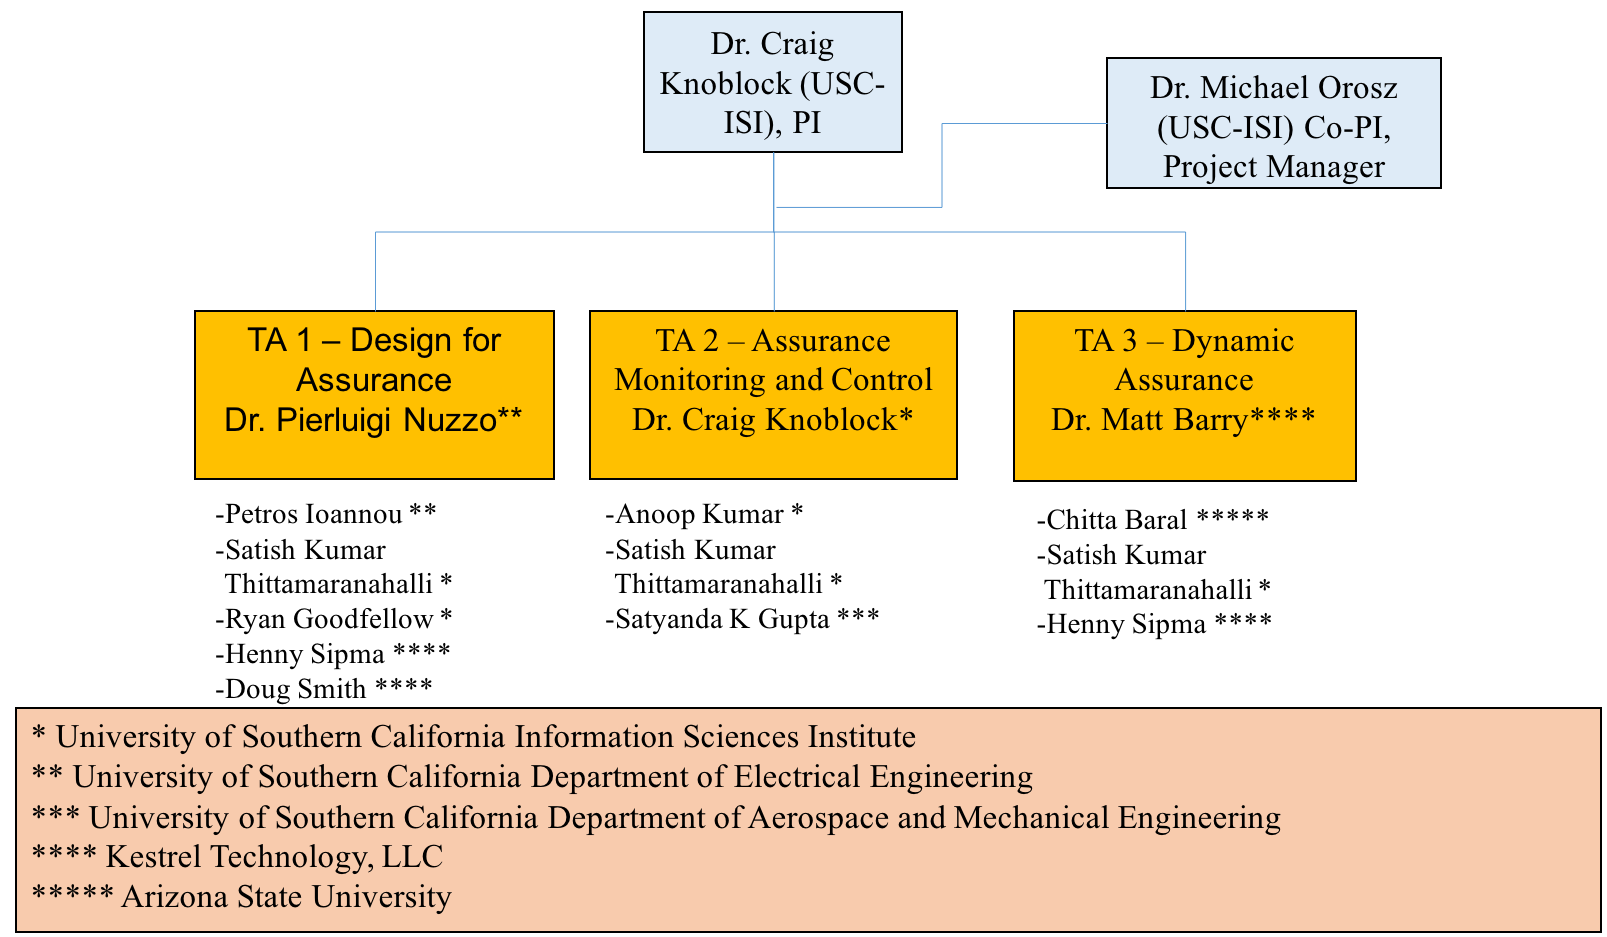
\includegraphics[width=6.0in]{./org-chart2.png}
\caption{\small Organization Chart}
\label{fig:org_chart}
\end{figure}

Coordination: To maximize collaboration and reduce risk to project failure from lack of communication and technical exchange, we plan to employ a wide variety of working styles and communication/coordination so that all can contribute.  At the core of our project will be regularly scheduled meetings bridging the diversely distributed team (Table~\ref{fig:Collaboration_Table}).  These meetings will address project status, identify challenges, implement risk mitigation strategies and participate in technology exchanges and system integration efforts (when appropriate)

\begin{table}[ht]
\caption{\small Project Meetings and Events}
  \centering
  {\footnotesize
\begin{tabular}{|m{3.15in}|m{3in}|} 
\hline
\textbf{Meeting} & \textbf{Frequency} 
\\\hline
Conference calls among investigators (discuss project status, address concerns and project risks) & Weekly
\\
\hline
Technical exchange and coordination meetings using Bluejeans or another videoconference technology & At least twice a month and more frequently as needed
  \\ 
\hline
Face-to-Face meetings (prior to P/I and demonstration meetings) & Every 3 to 6 months and more frequently (especially at the beginning of the project) as needed
 \\\cline{1-2}

\hline
\end{tabular}
}
\label{fig:Collaboration_Table}
\end{table}

\begin{table}[tbhp]
\caption{\small Key Project Team Member Responsibilities}
  \centering
  {\footnotesize
\begin{tabular}{| m{.75in} | m{3.9in}| m{1.5in}|} 
\hline
\textbf{Key Member} & \textbf{Responsibilities} & \textbf{Tasks} 
\\\hline
Dr.\ Craig Knoblock  & Principal Investigator responsible for project, leads TA 2 – Assurance Monitoring and Control.  Will lead the overall project and lead the TA2 team.  Served as the PI on many DARPA projects and has sucessfully led many large teams.    Effort on project:  25\% &
1.1.6, 1.2.2 1.2.3, 1.2.4, 1.3.4, 1.4.1, 
2.1.6, 2.2.2 2.2.3, 2.2.4, 2.3.4, 2.4.1, 
3.1.6, 3.2.2, 3.2.3, 3.2.4, 3.3.4, 3.4.1
\\
\hline
Dr.\ Michael Orosz & Co-Principal Investigator responsible managing the day-to-day operations of the project, assist technical teams as needed, coordinate with TA4 teams.    Has led many large complex multi-disciplined/multi-organizational projects in academic and industry environments.  Effort on project: 50\%
& 1.1.6, 2.1.6, 3.1.6, 1.4.1, 2.4.1, 3.4.1
  \\ 
\hline
Dr.\ Pierluigi Nuzzo 
& 
Co-Principal Investigator.  Leads the TA 1 - Design for Assurance team and conducts research on the formal methods for the design of the TA1 system.  Research experience on methodologies and tools for the design of cyber-physical systems; contracts, interfaces, and compositional methods for embedded system design; the application of automated formal methods and optimization theory to problems in embedded and cyber-physical systems.  Effort on project: 2 months/year (16.6\%)
& 
1.1.1, 2.1.1, 3.1.1 \\
\hline
Dr.\ Matthew Barry
& 
Key personnel.  Leads the TA 3 – Dynamic Assurance.   He will conduct the research on the dynamic assurance case language editors and parsers, the run-time system, and system integrations. Effort on project:  66\%
& 
1.3.2, 2.3.2, 3.3.2\\
\hline
Dr.\ Chitta Baral
& 
Key personnel responsible for learning assurance rules, supporting assurance rules with uncertainty and improving solver speed.  Expertise on ASP solvers, which will be used to reason about the assurance cases. Effort on project: 20\%
& 
1.3.1, 2.3.1, 3.3.1 \\
\hline
Dr.\ Doug Smith 
& 
Key personnel will support formal methods aspects of TA1, and lead the effort on abstract refinement. Expertise in field of automated correct-by-construction program generation.    Effort on project: 40\%
& 
1.1.5, 2.1.5, 3.1.5 \\
\hline
Dr.\ Henny Sipma
& 
Key personnel who will support the program verification tasks under TA1.  Will lead the effort on program verification.   Effort on project:  45\%
& 
1.1.5, 2.1.5, 3.1.5, 1.3.2, 2.3.2, 3.3.2 \\
\hline
Dr.\ Petros Ioannou
& 
Key personnel responsible providing and extending the assurance test bed, which will be available at the start of the project for autonomous vehicles.   Effort on project: 1 month/year (8.3\%)
& 
1.1.2, 2.1.2 (optional), 3.1.2 (optional)
\\
\hline
Dr.\ Satyandra Kumar Gupta
& 
Key Personnel providing autonomous command and control expertise to the TA-2 team.   Will lead the research on safety aware learning on TA2.   Past research on physics-aware decision making to facilitate automation.  Effort on project: 1 month/year (8.3\%)
& 
1.2.1, 2.2.1, 3.2.1 \\
\hline
Dr.\ Anoop Kumar 
& 
Key personnel providing support to the TA 2 project team.  Will lead the research on monitoring \& control and detecting distribution shifts.  Effort on project: 50\%
& 
1.2.1, 1.2.2, 1.2.3, 1.2.4, 2.2.1, 2.2.2, 2.2.3, 2.2.4, 3.2.1, 3.2.2, 3.2.3, 3.2.4\\
\hline
Dr.\ Satish Thittamaranahalli
& 
Key personnel developing scalable algorithms for TA1, TA2, and TA3 project teams.  Has extensive experience on scalable algorithm design, machine learning, and constraint reasoning.  Effort on project: 50\%
& 
1.2.1, 1.2.2, 1.2.3, 1.2.4, 2.2.1, 2.2.2, 2.2.3, 2.2.4, 3.2.1, 3.2.2, 3.2.3, 3.2.4, 1.1.4, 2.1.4, 3.1.4 \\
\hline
Dr.\ Ryan Goodfellow
& 
Key personnel providing support to the TA-1 project. Will lead the research on simulation-based testing.  Has extensive experience on simulation-based testing.  Effort on project:  30\%
& 
1.1.3, 2.1.3, 3.1.3 \\

\cline{1-2}

\hline
\end{tabular}
}
\label{fig:Table_Mgmt}
\end{table}



\newpage
\section{Personnel, Qualifications and Commitment}

{\bf Dr.\ Craig Knoblock}, the PI on this effort, is a Research Professor of both Computer Science and Spatial Sciences at the University of Southern California (USC) and Director of the Intelligent Systems Division at the USC Information Sciences Institute.   He received his Ph.D. from Carnegie Mellon University in computer science. 
%His research focuses on techniques for describing, acquiring, and exploiting the semantics of data.  
In previous projects he has worked on developing  scalable approaches to execution monitoring, accurate detection of sensor failures, and   automatic modeling and reconstruction of sensors.  He has published more than 300 journal articles, book chapters, and conference papers on these topics.  Dr. Knoblock is a Fellow of the Association for the Advancement of Artificial Intelligence (AAAI), a Distinguished Scientist of the Association of Computing Machinery (ACM), a Senior Member of IEEE, past President and Trustee of the International Joint Conference on Artificial Intelligence.
%and winner of the 2014 Robert S. Engelmore Award.  

{\bf Dr.\ Michael Orosz}, a Co-PI on this effort, is a Research Associate Professor of Civil and Environmental Engineering at the University of Southern California (USC) and Research Director of the Decision Systems Group at the USC Information Sciences Institute.  Dr. Orosz has over 30 years’ experience in commercial and government software development, basic and applied research, project management, academic research and has developed and deployed several commercially successful products.  His research interests are in machine learning and decision analytics as applied to intelligence analysis and autonomous command and control such as smart building controls.    Dr. Orosz has extensive experience in managing large complex multi-disciplined/multi-teamed research projects. %funded by DARPA, DHS, DoD, DoE, Industry, NASA, NRO, NSA and ONR.   
He received his Ph.D. in computer science from the University of California, Los Angeles.

{\bf Dr.\ Pierluigi Nuzzo}, a Co-PI on this project, is an Assistant Professor in the Department of Electrical Engineering at the University of Southern California. He received the Ph.D. in Electrical Engineering and Computer Sciences from the University of California at Berkeley. 
%in 2015, and the Laurea degree (MS) in electrical engineering (summa cum laude) from the University of Pisa, Italy, and the Sant'Anna School of Advanced Studies, Pisa, Italy.
%
%He has four years of research experience in analog and mixed signal circuit design as a researcher at IMEC, Leuven, Belgium, and over 10 years experience in design methodologies and tools for mixed-signal integrated circuits and cyber-physical systems, as a researcher at the University of Pisa, IMEC, UC Berkeley, and USC. 
His research interests
include: methodologies and tools for cyber-physical system and mixed-signal
system design; contracts, interfaces and compositional methods for embedded
system design; the application of formal methods and optimization theory to problems in embedded and cyber-physical systems and electronic design automation. 
%
Prof. Nuzzo received %First Place in the operational category and Best Overall
%Submission in the 2006 DAC/ISSCC Design Competition, 
a Marie Curie Fellowship
from the European Union in 2006, 
the University of California at Berkeley EECS
departmental fellowship in 2008, 
%the University of California at Berkeley Outstanding Graduate Student Instructor Award in 2013, 
the IBM Ph.D.
Fellowship in 2012 and 2014, 
%the Best Paper Award from the International Conference on Cyber-Physical Systems (ICCPS) in 2016, 
and the David J.~Sakrison Memorial Prize in 2016 for his doctoral research. 
%He is an author of 1 patent and over 60 publications.

{\bf Dr.\ Satyandra K. Gupta} is Smith International Professor in the Department of Aerospace and Mechanical Engineering at the University of Southern California. %Prior to joining the University of Southern California, he was a Professor in the Department of Mechanical Engineering and the Institute for Systems Research at the University of Maryland. He was the founding director of the Maryland Robotics Center and the Advanced Manufacturing Laboratory at the University of Maryland. 
He served as a program director for the National Robotics Initiative at the National Science Foundation from September 2012 to September 2014.  Dr. Gupta's interest is in the area of physics-aware decision making to facilitate automation. He has published more than 300 technical articles. He is a fellow of the American Society of Mechanical Engineers (ASME) and editor of ASME Journal of Computing and Information Science in Engineering. Dr. Gupta has received the Young Investigator Award from the Office of Naval Research in 2000, CAREER Award from the National Science Foundation in 2001, Presidential Early Career Award for Scientists and Engineers (PECASE) in 2001, Invention of the Year Award at the University of Maryland in 2007, Kos Ishii-Toshiba Award from ASME in 2011, and Excellence in Research Award from ASME in 2013.%, and Distinguished Alumnus Award from Indian Institute of Technology, Roorkee in 2014. %He has also received seven best paper awards at conferences.

{\bf Ryan Goodfellow} is a computer scientist at ISI working in combined cyber physical simulation and emulation platform development. His formal background is in simulation algorithms and modeling techniques using differential-algebraic equations (DAE). He has applied this knowledge in the CPS space by integrating DAE modeling languages and simulation engines with network testbeds to create comprehensive scientific experimentation platforms for cyber-physical systems. These experimentation platforms have been used in the power grid research space. %Ryan is a lead developer on the Deter network testbed, with a strong background in networked and distributed systems engineering. %He is also a combat veteran, serving as a non-commissioned officer and SIGINT team lead for a multi-functional intelligence team in Afghanistan.

{\bf Dr.\ Petros Ioannou} is a Professor in the Department of Electrical Engineering, Director of the Center for Advanced Transportation Technologies and Associate Director for Research for the DOT supported University Transportation Center at USC. He received his MS and PhD from the University of Illinois at Urbana Champaign in Mechanical and Electrical Engineering, respectively. His research interests are in robust adaptive control, vehicle dynamics and control, human factors and safety, automated vehicles, nonlinear systems and Intelligent transportation Systems.  He received the 2016 IEEE Transportation Technologies field award and the 2016 IEEE Control system society Transition to Practice Award. He is a Fellow of IEEE, IFAC and IET and author/coauthor of 8 books and over 400 papers.

{\bf Dr.\ Matthew Barry} will serve as lead for the TA3 tasks. %He will implement the dynamic assurance case language editors and parsers, the run-time system, and system integrations.  He will implement the assurance case arguments and the API for updating argument structure and content.  
Dr. Barry currently is CEO at Kestrel Technology LLC, and previously spent 20 years in NASA space mission operations at the Jet Propulsion Lab and Johnson Space Center.  At NASA Headquarters he led the introduction of dependability case requirements and plans for flight computing systems in upcoming manned space exploration missions, as well as the development of Agency-level software-related safety-critical control system requirements.  He recently served as a Principal Investigator on DHS/Cyber S\&T STAMP (Static Tool Analysis Modernization Program), DARPA CSFV (Crowd Sourced Formal Verification), three NASA Aeronautics R\&D projects, and the AFRL-sponsored Static Analysis of Numerical Algorithms project.  Dr. Barry earned BSME, MS, and PhD degrees in mechanical engineering, and an MBA degree, from Rice University.  

{\bf Dr.\ Henny Sipma} will support the program verification tasks under TA1.  %She is the key person behind the company's {\em KT Advance\/} and {\em KT Transferal\/} static analysis products, and the designer and programmer of the company's core {\em CodeHawk\/} abstract interpretation engine. 
Dr. Sipma currently is the CTO at Kestrel Technology LLC.  She has spent the past 10 years with Kestrel Technology as a static analysis expert; previously developed and taught static analysis techniques as senior research associate at Stanford University for eight years; and developed industrial process controls as an senior systems analyst at Shell.  She has been Principal Investigator or company lead on several recent R\&D projects for Federal agencies, including two projects under the IARPA STONESOUP (Securely Taking On New Executable Software of Uncertain Provenance) program; the DHS Cyber S\&T Gold Standard project; and the DARPA-sponsored STAC (Space-Time Analysis for Cybersecurity) and MUSE (Mining and Understanding Software Enclaves) programs.  Dr. Sipma earned 
%a BS degree in chemistry and an MS degree in chemical engineering at the University of Groningen in The Netherlands, and 
MS and PhD degrees in computer science from Stanford University.  

{\bf Dr.\ Douglas R.\ Smith} will support formal methods aspects of TA1, including the enforcement of safety properties and the generation of monitors.  He is President of Kestrel Technology LLC and Principal Scientist at Kestrel Institute.  He is a Fellow of the American Association of Artificial Intelligence (AAAI) and an ASE Fellow (Automated Software Engineering).  From 1986 to 2000, he taught an advanced graduate course on correct-by-construction software development at Stanford.  
%Dr. Smith has led the development of a series of software synthesis systems, including KIDS (Kestrel Interactive Development System), Specware, Designware, and Planware. 
%Applications domains have included a variety of complex high-performance planners and schedulers for the US Air Force.  He leads current projects on the generation of air mission plans and cyberoperations.  
Other recent projects focused on automated policy enforcement \cite{SmithD0703,SmithD08}, synthesis of secure network protocol codes, and the synthesis of high-performance constraint-solvers\cite{SmithD08c,SmithD13}.  Dr. Smith has over 30 years experience in the field of automated correct-by-construction program generation and has published over 100 papers. He has one patent.  He received the Ph.D. in Computer Science from Duke University% in 1979.  

{\bf Dr. Chitta Baral} is a Professor in the Department of Computer Science and Engineering at Arizona State University. He will support the TA3 efforts on Learning assurance rules, supporting assurance rules with uncertainty and improving solver speed. Dr. Baral has expertise in various aspects of autonomy and Artificial Intelligence. 
He wrote the first book on answer set programming (published by Cambridge University Press) the formal language behind our assurance rules. Some of his other works relevant to this proposal are: goal specification for autonomous systems, automatic construction of control rules for autonomous systems that satisfy given goals, combining machine learning with reasoning in various contexts, including image understanding. %He is the President of KR Inc. He is an associate editor of AIJ and has been an associate editor of JAIR.

{\bf Dr.\ Satish Kumar Thittamaranahalli (T. K. Satish Kumar)} leads the Collaboratory for Algorithmic Techniques and Artificial Intelligence (CATAI) at USC's Information Sciences Institute. He has published over 60 papers on numerous topics in Artificial Intelligence spanning such diverse areas as Constraint Reasoning, Planning and Scheduling, Probabilistic Reasoning, Robotics, Combinatorial Optimization, Approximation and Randomization, Heuristic Search, Model-Based Reasoning, Knowledge Representation and Spatio-Temporal Reasoning. %He %has served on the Program Committees of many international conferences in Artificial Intelligence
He and is a winner of the 2016 Best Robotics Paper Award and the 2005 Best Student Paper Award from the International Conference on Automated Planning and Scheduling. 
Dr. Kumar received his PhD in Computer Science from Stanford University. %In the past, he has also been a Visiting Student at the NASA Ames Research Center, a Postdoctoral Research Scholar at the University of California, Berkeley, a Research Scientist at the Institute for Human and Machine Cognition, a Visiting Assistant Professor at the University of West Florida, and a Senior Research and Development Scientist at Mission Critical Technologies.

\textbf{Dr.\ Anoop Kumar} is a senior computer scientist at USC ISI and has broad expertise in machine learning, statistical modeling, and software engineering.  Dr.\ Kumar is the technical lead on the DARPA RSPACE program and has played a vital role in developing a system that fuses air operations data from multiple sources, maintains world state, and issues warnings. Previously, he led the research and development of the BBN’s election forecasting system for the IARPA OSI program. %Dr.\ Kumar played a significant role in the DARPA DEFT program by developing a model to support integration of output from multiple NLP algorithms. He has contributed at the development to management levels on government research contracts and commercial projects. 
Dr.\ Kumar helped design and develop BBN's commercially available, hosted speech and medical transcription services offering. 

\begin{table}[!tbh]
\begin{footnotesize}
\vspace{-0.1in}

\begin{tabular}{lll}
\begin{tabular}[t]{|l|@{}c@{}|@{}c@{}|@{}c@{}|@{}c@{}|} \hline
Project & Status & \multicolumn{3}{ c| }{Hours} \\ \cline{3-5}
& & P1 & P2 & P3 \\ \hline



\multicolumn{5}{ |c| }{ \textbf{Craig Knoblock} } \\ \cline{1-5}
Safeguard & Pro & 770 & 641 & 641 \\ \cline{1-5}
ELICIT & Cur & 308 & 256 & 120 \\ \cline{1-5}
WTNIC & Cur & 11 & 0 & 0 \\ \cline{1-5}
EFFECT & Cur & 641 & 107 & 0 \\ \cline{1-5}
LinkedMaps & Cur & 203 & 25 & 0 \\ \cline{1-5}
PRINCESS & Cur & 608 & 96 & 0 \\ \cline{1-5}
SCHARP & Cur & 481 & 54 & 0 \\ \cline{1-5}
MINT & Pen & 650 & 534 & 285 \\ \cline{1-5}

\multicolumn{5}{ |c| }{ \textbf{Michael Orosz} } \\ \cline{1-5}
Safeguard & Pro & 1560 & 1300 & 1300  \\ \cline{1-5}
SMC/SY & Cur & 1803 & 0 & 0  \\ \cline{1-5}

\multicolumn{5}{ |c| }{ \textbf{Matthew Barry} } \\ \cline{1-5}
Safeguard & Pro & 2078 & 1690 & 1554 \\ \cline{1-5}
Starlite & Cur & 1840 & 1692 & 0 \\ \cline{1-5}



\multicolumn{5}{ |c| }{ \textbf{Anoop Kumar} } \\ \cline{1-5}
Safeguard & Pro & 1560 & 1300 & 1300 \\ \cline{1-5}

\end{tabular}
&
\begin{tabular}[t]{|l|@{}c@{}|@{}c@{}|@{}c@{}|@{}c@{}|} \hline
Project & Status & \multicolumn{3}{ c| }{Hours} \\ \cline{3-5}
& & P1 & P2 & P3 \\ \hline

\multicolumn{5}{ |c| }{ \textbf{Pierluigi Nuzzo} } \\ \cline{1-5}
Safeguard & Pro & 520 & 433 & 433  \\ \cline{1-5}
Mirage & Cur & 433 & 0 & 0  \\ \cline{1-5}

\multicolumn{5}{ |c| }{ \textbf{Satyandra Gupta} } \\ \cline{1-5}
Safeguard & Pro & 260 & 217 & 217 \\ \cline{1-5}
Human   & Cur & 22 & 0 & 0 \\ \cline{1-5}
Vehicles & Cur & 36 & 0 & 0 \\ \cline{1-5}
Robot & Cur & 116 & 0 & 0 \\ \cline{1-5}
Assembly & Cur & 33 & 0 & 0 \\ \cline{1-5}
Solar & Cur & 4 & 0 & 0 \\ \cline{1-5}

\multicolumn{5}{ |c| }{ \textbf{Petros Ioannou} } \\ \cline{1-5}
Safeguard & Pro & 260 & 217 & 217 \\ \cline{1-5}
CPS & Cur & 130 & 0 & 0 \\ \cline{1-5}

\multicolumn{5}{ |c| }{ \textbf{Ryan Goodfellow} } \\ \cline{1-5}
Safeguard & Pro & 936 & 780 & 780 \\ \cline{1-5}
STEAM & Cur & 416 & 0 & 0 \\ \cline{1-5}


\end{tabular}
&
\begin{tabular}[t]{|l|@{}c@{}|@{}c@{}|@{}c@{}|@{}c@{}|} \hline
Project & Status & \multicolumn{3}{ c| }{Hours} \\ \cline{3-5}
& & P1 & P2 & P3 \\ \hline

\multicolumn{5}{ |c| }{ \textbf{Chitta Baral} } \\ \cline{1-5}
Safeguard & Pro & 659 & 485 & 485 \\ \cline{1-5}
PostdocBP & Cur & 176 & 0 & 0 \\ \cline{1-5}
Languages & Pen & 528 & 264 & 264 \\ \cline{1-5}
CAREER & Pen & 88 & 44 & 44 \\ \cline{1-5}
CHS & Pen & 510 & 255 & 0 \\ \cline{1-5}

\multicolumn{5}{ |c| }{ \textbf{Doug Smith} } \\ \cline{1-5}
Safeguard & Pro & 1222 & 984 & 840 \\ \cline{1-5}
RSPACE & Cur & 342 & 0 & 0 \\ 
\cline{1-5}
PLANX & Cur & 154 & 0 & 0 \\ 
\cline{1-5}
HACCS & Pen & 923 & 769 & 769 \\ 
\cline{1-5}

\multicolumn{5}{ |c| }{ \textbf{Henny Sipma} } \\ \cline{1-5}
Safeguard & Pro & 1372 & 962 & 840 \\ \cline{1-5}
STAC & Cur & 797 & 0 & 0 \\ \cline{1-5}

\multicolumn{5}{ |c| }{ \textbf{Satish Thittamaranahalli} } \\ \cline{1-5}
Safeguard & Pro & 1560 & 1300 & 1300 \\ \cline{1-5}
MapF & Cur & 103 & 103 & 0 \\ \cline{1-5}

\end{tabular}
\end{tabular}

\end{footnotesize}
\caption{Individual commitments of key personnel}
\label{tab:Commitments}
\vspace{-0.2in}
\end{table}

\clearpage
\newpage
\section{Capabilities}


%\subsection{University of Southern California}
USC has strengths in number of areas that are closely related to the proposed work:
\begin{itemize}[itemsep=0pt,leftmargin=*]
\item Dr.\ Nuzzo 
%has over 10-year research experience in embedded system design, from mixed-signal chip design (analog-to-digital converters, frequency synthesizers, software-defined radio), to methodologies and tools for mixed-signal integrated circuits and Cyber-Physical Systems (CPSs), and the application of formal methods and optimization theory to problems in embedded and cyber-physical systems and electronic design automation.  
%His doctoral work 
has done extensive research on contracts and compositional methods for heterogeneous system design and design space exploration, with application to aircraft electric power systems and environmental control systems. His work has helped transition rigorous system design foundations, innovative design methodologies, and new systems engineering paradigms to industry (IBM, United Technologies). 
\item Dr.\ Satyandra K. Gupta has worked on autonomous surface vehicles, autonomous ground vehicles for operation on rugged terrains, and autonomous flapping wing aerial vehicles.   His group has developed a hierarchal decision making approach for realizing autonomous systems. 
%This approach combines task planning and assignment, deliberative trajectory planning, reactive collision avoidance behaviors, and trajectory tracking control layers. 
His group has also developed new methods for learning reactive behaviors in adversarial environments and COLREGS compliant trajectory planning. \item Dr.\ Knoblock has developed methods that learn the relationships between sensors to both identify failures and changes in sensor and reconstruct those sensors, providing estimates of the accuracy of the reconstructed sensors.  
\item Ryan Goodfellow has extensive experience in simulation based testing through high-fidelity CPS testbed environment development and operation, using the Deter network testbed as the core which has supported several large scale government projects from a variety of agencies and thousands of users. %we have developed sophisticated CPS experiments under programs such as NFS RIPS, NIST SmartCities and the DHS Cybersecurity showcase.
\item Dr.\ Ioannou %helped  design and implement adaptive cruise control systems in collaboration with Ford Motor Company, which was commercialized four years before any other company. He 
worked on several DOT funded projects on automated vehicles and intelligent highway systems where he demonstrated his vehicle control designs for safety and performance on actual automated vehicles in test trucks and I-15 highway.
\item Drs.\ Knoblock, Kumar, and Thittamaranahalli have developed highly scalable approaches for monitoring message traffic to identify potential problems and issue warnings and alerts. 
\item Dr. Thittamaranahalli has developed state-of-the-art methods for efficiently solving large-scale search and optimization problems. %These techniques will be applicable in TA2 for safety-aware learning and planning, in TA2 for assurance monitoring and control, and in TA3 for dynamic assessment of assurance cases.

\end{itemize}
%\subsection{Kestrel Technology LLC}

Kestrel Technology's strength is in program analysis, specifically static analysis of both source and binary targets.  The company performs applied R\&D and product development for a variety of static analysis applications  pivoting primarily on the abstract interpretation technique.  The company recently initiated development of program analysis applications using logical equivalence techniques. As a provider of verification evidence in the form of mathematical proofs, the company also has expertise in the design and development of assurance case arguments for high-integrity systems using such evidence. %The company is engaged in a partnership with Wind River Systems to develop program analysis tools for its embedded system developers.  Many of Wind River's customers must develop their products under safety and certification standards, including those using safety cases.  

   

%\subsection{Arizona State University}
Chitta Baral at Arizona State University has developed various software to learn assurance rules and various ASP solvers, which he has made available as open-source.

Most of the software carried forward for implementation or derivation is open source.  The single exception is Kestrel Technology's {\it KT Advance\/} static analysis tool (TA1), in particular the abstract interpretation engine therein, which is company proprietary and is US EAR export-controlled.   
%Owing to mixed funding for the development of that technology 
We will continue to provide the Federal government a restricted use license for that particular item.

There are no specialized facilities, data, or GFE required for this effort. 

\include{sow}
\include{milestones}

% \section{Level of Effort by Task \textcolor{red}{[Mike/Lisa - 1 pages]}}

% \textcolor{blue}{
% \begin{itemize}
% \item Will be a separate spreadsheet
% \item
% \end{itemize}
% }

\include{appendix_a}

%\section{Appendix B \textcolor{red}{[No Page Count]}}

\section{References}
\bibliographystyle{acm} 
\bibliography{TA3/ta3,TA2/ta2,TA1/ta1}
\end{document}
%%\documentclass[a4paper]{article}
%\documentclass[12pt]{article}
\documentclass[12pt]{dod-blank}

%% Language and font encodings
\usepackage[english]{babel}
\usepackage[utf8x]{inputenc}
\usepackage[T1]{fontenc}

%% Sets page size and margins
%%\usepackage[a4paper,top=3cm,bottom=2cm,left=3cm,right=3cm,marginparwidth=1.75cm]{geometry}
%\usepackage[top=1in, bottom=1in, left=1in, right=1in]{geometry}



%% Useful packages
\usepackage{amsmath}
\usepackage{graphicx}
  \graphicspath{{.}{./image/}}
  \DeclareGraphicsExtensions{.png,.jpg} 
\usepackage[colorinlistoftodos]{todonotes}
\usepackage[colorlinks=true, allcolors=blue]{hyperref}
\usepackage{tabularx}
\usepackage{multirow}
\usepackage{tabulary}
\usepackage{float}
\usepackage{wrapfig}
\usepackage[export]{adjustbox}
\usepackage{comment}
\usepackage{tabularx}
\usepackage{multirow}
\usepackage{tabulary}
\usepackage{enumitem}

\usepackage{listings}
\usepackage{color}
\usepackage{array}
\usepackage{subcaption}
\usepackage{xcolor}




\renewcommand{\textfraction}{0}
\renewcommand{\topfraction}{1.0}
\renewcommand{\bottomfraction}{1.0}

\usepackage{longtable}
%% macros
\newif\iffinal
\finaltrue
\iffinal
  
    \newcommand\baareq[1]{}
    \newcommand\baades[1]{}
 
 
\else
    \definecolor{darkgreen}{rgb}{0,0.4,0}
    \definecolor{darkcyan}{rgb}{0,0.4,0.4}
    \definecolor{darkblue}{rgb}{0,0,0.5}
    
    \newcommand\baareq[1]{{\color{darkcyan}[\textbf{Requirement:} #1]}}
    \newcommand\baades[1]{{\color{darkcyan}[\textbf{Description:} #1]}}
 
\fi




\def\naive{na\"{\i}ve}



\lstset{ 
  backgroundcolor=\color{white},   % choose the background color; you must add \usepackage{color} or \usepackage{xcolor}
  basicstyle=\footnotesize\ttfamily,            % the size of the fonts that are used for the code
  breakatwhitespace=false,         % sets if automatic breaks should only happen at whitespace
  breaklines=true,                 % sets automatic line breaking
  captionpos=b,                    % sets the caption-position to bottom
  commentstyle=\color{mygreen},    % comment style
  % deletekeywords={...},            % if you want to delete keywords from the given language
  escapeinside={\%*}{*)},          % if you want to add LaTeX within your code
  extendedchars=true,              % lets you use non-ASCII characters; for 8-bits encodings only, does not work with UTF-8
  frame=single,	                   % adds a frame around the code
  keepspaces=false,                 % keeps spaces in text, useful for keeping indentation of code (possibly needs columns=flexible)
  keywordstyle=\color{blue}\bfseries\underbar,       % keyword style
  language=Prolog,                 % the language of the code
  % morekeywords={if,and},        % if you want to add more keywords to the set
  numbers=none,                    % where to put the line-numbers; possible values are (none, left, right)
  numbersep=5pt,                   % how far the line-numbers are from the code
  numberstyle=\tiny\color{mygray}, % the style that is used for the line-numbers
  rulecolor=\color{black},         % if not set, the frame-color may be changed on line-breaks within not-black text
  showspaces=false,                % show spaces everywhere adding particular underscores; it overrides 'showstringspaces'
  showstringspaces=false,          % underline spaces within strings only
  showtabs=false,                  % show tabs within strings adding particular underscores
  stepnumber=2,                    % the step between two line-numbers. If it's 1, each line will be numbered
  stringstyle=\color{mymauve},     % string literal style
  tabsize=2,	                   % sets default tabsize to 2 spaces
  title=\lstname                   % show the filename of files included with \lstinputlisting; also try caption instead of title
}

% apply trick for additional keywords for our AC DSL
\lstset{
	emph={for, if, and, or},
    emphstyle={\color{blue}\bfseries\underbar}
}




\title{DARPA Assured Autonomy}
\author{Technical Volume- \textcolor{red}{Thirty-Eight (38) pages max}}

\begin{document}
\pagenumbering{roman}
\include{cover}

\newpage
\section{Table of Contents}
\tableofcontents

\newpage
\pagenumbering{arabic}
\section{Executive Summary}
As we rapidly move into a world where machine learning plays a central role in realizing autonomous systems, it is becoming increasingly important to develop techniques that assure that these systems will operate safely and perform as expected. Current approaches are limited to providing assurance for systems with limited or no  learning capabilities. In this context, DARPA's Assured Autonomy BAA seeks to \emph{develop rigorous design and analysis technologies for continual assurance of learning-enabled autonomous systems}. USC in collaboration with Kestrel Technology and ASU is pleased to submit a comprehensive TA1, TA2, and TA3 proposal entitled \emph{``Assured Autonomy for Learning Enabled Vehicles (Safeguard).''} We plan to provide an end-to-end solution to support autonomous systems with learning-enabled components, ranging from design technologies for assurance, to assurance monitoring and control techniques, to representation and online evaluation of assurance cases. We have assembled a strong team of experts that cover the range of technologies that are required to create such an end-to-end system. If successful, the project will provide the technologies for building the next-generation of learning-enabled autonomous systems.  The entire project will take four years and cost \textcolor{red}{\$??}, with an initial version completed at the end of Phase I and successive versions with additional capabilities and improved scalability at the end of Phase II and Phase III.  

In the remainder of this section, we first introduce an  unmanned surface vehicle scenario that will be used throughout the proposal to describe the approach.  Next, we describe our approach to design, monitoring, and dynamic assurance. Finally, we introduce the team involved in the project. 

\textbf{Motivating Scenario.} Consider an autonomous unmanned surface vehicle (USV) guarding a valuable asset in the ocean when an unknown vehicle  approaches the security perimeter, under challenging weather conditions. In this scenario, the USV is required to approach the intruding vehicle, issue a warning signal, and escort it to a safe distance from the controlled area. However, as the USV has no a priori knowledge of its external environment behaviors (e.g., water depth, waves, wind, current, visibility), pre-computing a feasible trajectory, let alone optimal, becomes a non-trivial problem. For trajectory planning, the USV must continuously perform the following tasks:
\begin{itemize}[itemsep=0pt,leftmargin=*]
 \item Sense the current state of the surrounding environment (e.g., water depth, waves, wind, current, visibility) and estimate its own maneuverability constraints (e.g., braking distance, available acceleration, maximum velocity, turning radius, turning rate, safety distance) based on the state of the environment;      
\item Sense the static obstacles in the sensor range and generate a traversability map;
\item Sense the moving obstacles and classify them;   
\item Predict future trajectories of moving obstacles; 
\item Determine if any of the COLREGS \cite{commandant1999international} rules will be in effect with respect to one or more of the nearby vessels and identify the vessels with the right of way.    
\end{itemize}
The above information will be used by the trajectory planner to compute an initial trajectory, which will be continuously refined as the USV gathers additional information.
% It is not possible for the USV to be tested in every possible environment. 
The USV will use learning enabled components to take  decisions as it encounters new situations, such as  
\begin{itemize}[itemsep=0pt,leftmargin=*]
\item Classifiers to identify moving obstacles based on physical appearance and motion signatures,
\item Algorithms to estimate the sensor capabilities in adverse weather conditions,   
\item Algorithms to accurately estimate uncertainty in the environment, 
\item Classifiers to generate traversability maps,
\item Prediction of external vessel behaviors based on motion histories, 
\item Reinforcement learning  to ensure COLREGS compliance of maneuvers,  
\item Algorithms to learning pursuit behaviors.  
\end{itemize}
Learning enabled components will interact with each other in complex ways, where a misclassification error in one component may eventually compromise the entire mission.   
% We will need to make sure that each learning enabled components has a run-time monitor that will ensure that the assumptions made by the learning-enabled component remain valid and prevent erroneous learning. 
% For example, if the vehicle is exhibiting significant error in trajectory tracking, then simply downgrading the trajectory tracking error value may not be a good option.  The failure of prediction of trajectory tracking error might be due to the presence of a significant wake caused by a nearby vessel. The presence of the nearby vessel can be used to explain the degradation in trajectory tracking performance. As the vessel moves away, we can expect the trajectory tracking performance to return to the predicted level.  
While exhaustive validation of learning-enabled cyber-physical systems (LE-CPSs) is a prohibitive task~\cite{Kalra16},
their complexity, heterogeneity, and highly dynamic nature
make it challenging to even leverage existing model-based development techniques to effectively assess system correctness 
% dependability, 
at design time or enforce it at runtime.

\textbf{Design for Assurance.} Safeguard uses a platform-based design approach~\cite{Nuzzo15b} to organize the design process for a LE-CPS and to build assurance cases. Composite models are developed at several levels of abstraction,
from top-level system requirements and safety constraints down to the
implementation level.  Intermediate levels add detail to the levels
above.  The different levels are connected by refinement mappings that
allow properties established at one level to be preserved at the next
level (see Figures~\ref{fig:methodology} and~\ref{fig:assurance}).

Contracts are used to formally specify components and composite models
in terms of (1) Assumptions -- the assumed behaviors of the
environment and the behaviors of other components, and (2) Guarantees
-- the behavior properties that a model guarantees if it operates in a
context that satisfies its assumptions.  A calculus of contracts
allows horizontal composition of contracts to generate contracts for
composite models.  Vertical contracts are used to specify the mapping
or refinement relation between models at different levels of
abstraction.  The system design process starts with a high-level
contract that expresses overall system assumptions and requirements.
Subsequent levels express models with increasing detail until the
lowest level expresses the system in terms of hardware components and
their software controllers.

The assurance case for a CPS arises from the horizontal and vertical
structure of the design in several ways.  The components used within a
particular level are either (1) synthesized using
correct-by-construction design tools together with proofs, (2) derived
statically or dynamically using safety-aware machine-learning
techniques, (3) written manually and verified by analysis tools, or
(4) written manually and validated by extensive testing.  The
assurance case for the whole reflects its compositional structure.  We
anticipate that well-specified contracts together with the calculus of
contracts will eliminate well-known problems with unexpected emergent
behaviors in CPS systems.

The assurance case for the lowest-layer design arises from both the
intra-level assurance and from properties and their proofs that are
preserved under the refinement mapping from the top-level
requirements.  The refinement mappings between model layers will be
constructed using a variety of techniques.  A contract at an abstract
level can be mapped to a component or refined contract by (1)
retrieval of pre-verified components from a platform library, (2)
synthesis using correct-by-construction design and optimization tools,
or (3) manual coding to satisfy a contract.  The mapping of a
composite model will be composed from the mappings of its constituent
components or contracts.  When a composite model cannot be mapped
compositionally to the next level, it will be generated using
correct-by-construction design and optimization tools.

\textbf{Assurance Monitoring and Control.}
We provide an integrated framework for safety-aware learning, assurance monitoring and control, detecting distribution shifts. Three major components offer an efficient TA2 architecture as well as interfaces with TA1 and TA3, that is, (a) safety-aware learning and planning, (b) assurance monitors for guarding architectural and safety constraints; and (c) distribution shift detection.

We will develop a new learning-enabled online decision-making framework that allows opportunistically composing a sequence of actions (maneuvers) to reduce uncertainty in the system capability model without suspending the progress toward the mission goals or compromising safety. Each candidate action is evaluated based on three criteria: (1) the risk of violating a safety constraint using the current uncertainties in the parameter estimates; (2) its relevance to the mission goals; (3)  its expected information gain, i.e., reduction in uncertainty, with respect to the parameter estimates. These evaluations are combined to produce a cumulative mission utility value for each action that drives our learning-enabled decision-making framework. The problem of generating and evaluating sequences of actions can be posed in several way. For example, it can be solved using a branch-and-bound search method like Anytime A*, or formulated with the finite-horizon Markov Decision Process (MDP) framework. We will develop new scalable search strategies to solve this problem efficiently, by potentially evaluating a recent method developed at USC, called FastMap, that can significantly improve the execution time. 

We will develop monitors for architectural and safety constraints. 
% While these constraints can be checked over and over again as sensor information flow in, this naive strategy accounts for a lot of computational overhead. 
To achieve scalability and decrease the overhead, we propose the application of a technique that we currently use in DARPA's RSPACE program, which leverages a physical model of the vehicles dynamics and its interactions with the environment to efficiently determine the readout frequency. We propose two  extensions of this basic idea. First, we will use the theory of Variable Elimination to prioritize which variables to monitor, e.g., controllable, versus uncontrollable, adversarially controlled, or unobservable variables. Second, we invoke the dynamic assessment of assurance cases only when needed. This  decreases the number of times dynamic assessment of assurance cases is initiated as well as the communication bandwidth between the TA2 and TA3 components.

Finally, we will identify a distribution shift by combining statistical and machine learning techniques to differentiate between environmental and sensor changes. We will exploit a categorization of the shifts based on their cause and duration as well as extend our earlier work on detecting and mitigating sensor failures for all types of monitored variables.  

\textbf{Dynamic Assurance:} The Safeguard {\em design for assurance\/} activity takes a systems-theoretic stance toward safety.  Consequently, it presumes that safety is an emergent property of the system, and that hazards can present themselves through unintended interactions and performance violations in addition to causal events such as component failures.  Our design approach includes consideration of intent as well as hazard analysis and mitigation.  The artifacts from these activities populate contracts and assumptions for the dynamic assurance case.  
We thus build safety into the product by working at a systems-level viewpoint, using lexicon and design patterns familiar to both hardware and software engineers; safety is an emergent property of the system, not an afterthought.  
As system behavior evolves during runtime owing to learning, threats, degradation, or some other factor, the dynamic assurance case identifies whether the safety constraints continue to be satisfied.  If not, it provides notifications or issues recovery instructions directly from a lookup table.

Our implementation of the dynamic assurance case employs a declarative knowledge base inference engine and a domain-specific language tailored to our approach.  We have used them successfully for assurance case tool sets and arguments, and will extend them to reason about uncertainty and learning.  Our approach to achieve scalability is to specialize solvers toward modularity and to take advantage of domain knowledge.  Specifically, we will develop answer set programming techniques for context-dependent learning for reasoning about the learning-enabled components as well as learning assurance rules.  We will develop new formalisms for uncertainty to include causality, using weights for computing probabilities, and probabilistic non-monotonicity.  To achieve scaling objectives we will implement specializations using modularity, weighted CSPs, and message passing. 

% The system safety constraints revealed from that design become the key elements of our dynamic assurance case.  Our verification tools ensure the constraints are relevant, identifiable, and their implementation and effect observable.  

\textbf{Team.} We have assembled a team that is exceptionally well-qualified to build the proposed Safeguard system.  The team will be led by Dr.\ Craig Knoblock, the Principal Investigator for the effort, who currently leads the Intelligent Systems Division at the Information Sciences Institute.  He has led many large DARPA and IARPA projects over the years and has a strong track record in conducting leading edge research and then transitioning the technology to commercial use.  He will be supported by Dr.\ Michael Orosz as the Project Manager, who also has  experience in managing large research projects and on autonomous systems.  The TA1 team will be led by Dr.\ Pierluigi Nuzzo, who is an expert in embedded system design methodologies and the  application of formal methods to cyber-physical systems.  The TA1 team also includes Dr.\ Doug Smith, who has spent many years working on scalable correct-by-construction techniques and Dr.\ Henny Sipma, who has significant experience in applying program verification methods to real-world problems.  The TA1 team also includes Ryan Goodfellow, who has done a large amount of work on simulation-based testing.  The TA2 team will be led by Dr.\ Knoblock who has worked on topics related to both monitoring and detecting distribution changes.  He will be supported by Dr.\ Satyandra Gupta, who is an expert on autonomous surface vehicles as well as on safety-aware learning. He will also be supported by Drs.\ Anoop Kumar and Satish Thittamaranahalli, who have also previously worked on efficient methods for execution monitoring.  The TA3 team will be lead by Dr.\ Matthew Barry, who has experience in creating the technologies for assurance cases.  He will be supported by Dr.\ Chitta Baral, who is an expert on ASP solvers and by Dr.\ Thittamaranahalli who is an expert on SAT solvers, both of which will be applied to provide scalable assurance case reasoning.  Finally, Dr.\ Petros Ioannou, who is an expert on control systems for autonomous vehicles will provide an autonomous vehicle platform, which will form the focus of our work until the TA4 teams provide additional vehicle platforms for development.  

\newpage
\section{Innovative Claims and Deliverables}

In this project we will develop and build an end-to-end system for assured autonomy.  This section describes the key innovations by technical area and then the overall deliverables of the project.

\paragraph{Design for Assurance}

\begin{itemize}[itemsep=0pt,leftmargin=*]
\item We address the LE-CPS design challenges via a holistic approach that can contextually generate design artifacts and assurance cases. We develop a compositional, contract-based modeling framework, methods, and tools to support the design process from system-level requirement capture,  formalization, and analysis, to the generation, testing, and continual monitoring of software and hardware artifacts in feedback loop with a physical process.

\item We develop compositional abstractions and interfaces (vertical contracts) that can  bridge heterogeneous formalisms and heterogeneous decomposition architectures to make system analysis and synthesis tractable, consistently combine different verification and synthesis methods at design time, and provide seamless support for dynamic assurance at run time. %We aim to quantitatively capture the confidence in the satisfaction of requirements under uncertain or unknown conditions, and resilience properties of  systems at different abstraction levels, to enable trade-off evaluation between resilience, performance, and cost.

\item We develop a unifying framework and efficient algorithms to reason about the combination of discrete and continuous dynamics and constraints in the presence of uncertainties in LE-CPS using a satisfiability modulo convex approach~\cite{Shoukry2017} for contract-based system verification and scalable trajectory planning.  

\item We provide an environment for high-fidelity CPS testing, in which production-ready software, e.g.,  safety-critical learning and control, may be deployed and tested 
% by extending the Cypress testbed environment \cite{Goodfellow2015Cypress:Systems} 
with time dilation facilities, so that it synchronizes with a physical simulation that is not necessarily running in real time, while still having the perception of real time.

\item We 
% These facilities allow a cyber system to be  
propose an approach for unanticipated behavior space identification and test coverage maximization which leverages results from the theory of differential algebraic equation (DAE)~\cite{Berger2013ControllabilitySurvey,Ilchmann2005ATheory,BergerOnSystems,Lamour2013} 
to prune the behavior search space and identify smaller regions of interest for efficient simulation-based testing. 
% We then compute the intersection of these two behavior spaces and restrict our simulation based testing search space to this subspace.
\end{itemize}

\paragraph{Assurance Monitoring and Control}

\begin{itemize}[itemsep=0pt,leftmargin=*]
\item 
%We integrate safety-aware learning into the overall decision making problem. The goal is to maximize mission utility without violating the safety constraints. 
Our safety-aware learning framework enables the system to opportunistically select and execute actions to assist the learning-enabled component in reducing model uncertainty without compromising safety or deviating from the mission goals. The value of uncertainty reduction is explicitly incorporated in the optimization process for selecting the best action.  
\item For safety-aware learning, we propose the idea of preprocessing the search space of the problem domain before queries and observations come in. With such a linear-time preprocessing phase, the performance of search and optimization algorithms can be significantly boosted. For example, in regular A* search, the intensional or extensional search space can be preprocessed in near-linear time to yield an embedding of each state as a point in Euclidean space~\cite{cujakk}. Then, when the query comes in, A* search can make use of these Euclidean distances as heuristic distances between two states to yield order-of-magnitude speedups. 
%In Anytime A* for safety-aware learning and planning, this leads to a significantly better quality of actions chosen within a time limit, and in the MDP framework, the same ideas can be used to improve the convergence of Bellman updates for safety-aware Reinforcement Learning.
\item As massive amounts of sensor information flow in, it is imperative for us to efficiently process this information for monitoring architectural and safety constraints. Building on our past work on similar tasks, we propose novel technologies for efficiently monitoring constraints. These algorithms can yield an exponential reduction in the amount of sensor data that needs to be processed. Doing this also reduces the message complexities between the various modules. %We also propose to use the theory of Variable Elimination (VE) to monitor constraints with uncontrollable, adversarially controlled, and/or unobservable variables. VE yields a substrate constraint to monitor that characterizes a dominant strategy of the controllable variables over the uncontrollable, adversarially controlled, and/or unobservable variables.
\item We will develop techniques to identify  distributional shifts and determine the underlying cause (e.g., change in environment, sensor failure,   etc.), as well as strategies for handling the various distributional shifts.   Notably, we propose to build on our past work and use compact representations to exploit historical data to identify distributional shifts.
\end{itemize}

\paragraph{Dynamic Assurance}

\begin{itemize}[itemsep=0pt,leftmargin=*]

\item We demonstrate the integration of dynamic assurance for safety-critical learning-enabled dynamic systems in which evolutionary behaviors are expected and tolerated as a property of the functionality.   The impact will be consequential contributions safety-critical dynamic systems in which evolutionary behaviors are expected and tolerated as portion of the functionality.   
\item We implement dynamic assurance by combining features of system safety, formal methods, logic programming, uncertain reasoning, and domain-specific languages.  We populate assurance case arguments at several levels of modeling and implementation abstraction, using the analysis results to produce design-time evidence supporting assurance claims.  
%We provide automated reasoning about the assurance case itself to produce verification, consistency, and completeness results for the argument.  Dynamic assurance results then yield trusted explanations of whether safety constraints and assumptions and other contracts still hold during the collection of runtime evidence from monitors. 
\item We develop and demonstrate ASP formalisms crucial to applications in dynamic assurance. We demonstrate the suitability of the technology especially for assurance case arguments owing to the improved legibility, consistency and completeness checks, handling of uncertain and default reasoning, and scalability.  
%We will produce modularized solvers for enhanced performance based on recent algorithmic developments in exploiting structure, kernelization, and message passing. We provide a formalism to enable learning of assurance rules. 
We provide a novel approach to handling uncertainty that provides the ability to do causal and counter-factual reasoning as well as probabilistic non-monotonicity.  Overcoming limitations of traditional inductive logic techniques, we develop a novel iterative and incremental approach based on context dependent learning. 
\end{itemize}

\paragraph{Deliverables}
During the course of this project, we will build and deliver a fully-operational system that covers all three of the technical areas.  The detailed capabilities of this system are described in the individual technical sections.  The resulting system will be available as open source under a permissive license, which will allow other organizations to use the work, extend it in new directions, and even commercialize the software.  Kestrel Technology has significant experience in this space and has built and applied these types of technologies to a variety of real world tasks.  Kestrel is ideally suited to pursue commercial uses of this technology and the permissive license will facilitate exploring these opportunities since there will be no need to negotiate intellectual property rights.  

\newpage
\section{Technical Plan}
\input{./TA1/main}
\input{./TA2/main}
\input{./TA3/main}
\clearpage
\newpage


\section{Management Plan}


The Principal Investigator for this effort is Dr. Craig Knoblock who is responsible for all aspects of the effort, will coordinate the parallel team efforts, and will ensure high levels of performance from individual team members.  The Co-P/I, Dr. Michael Orosz, will provide project management and will assist all performers in the execution of the project.    The project team is divided into three working groups (Figure~\ref{fig:org_chart}) corresponding to Technical Areas 1-3, however, members of each team contribute across all project activities.   Table~\ref{fig:Table_Mgmt} defines the major contributions of each project team member to the project tasks.

\begin{figure}[tbhp]
%\vspace{-25pt}
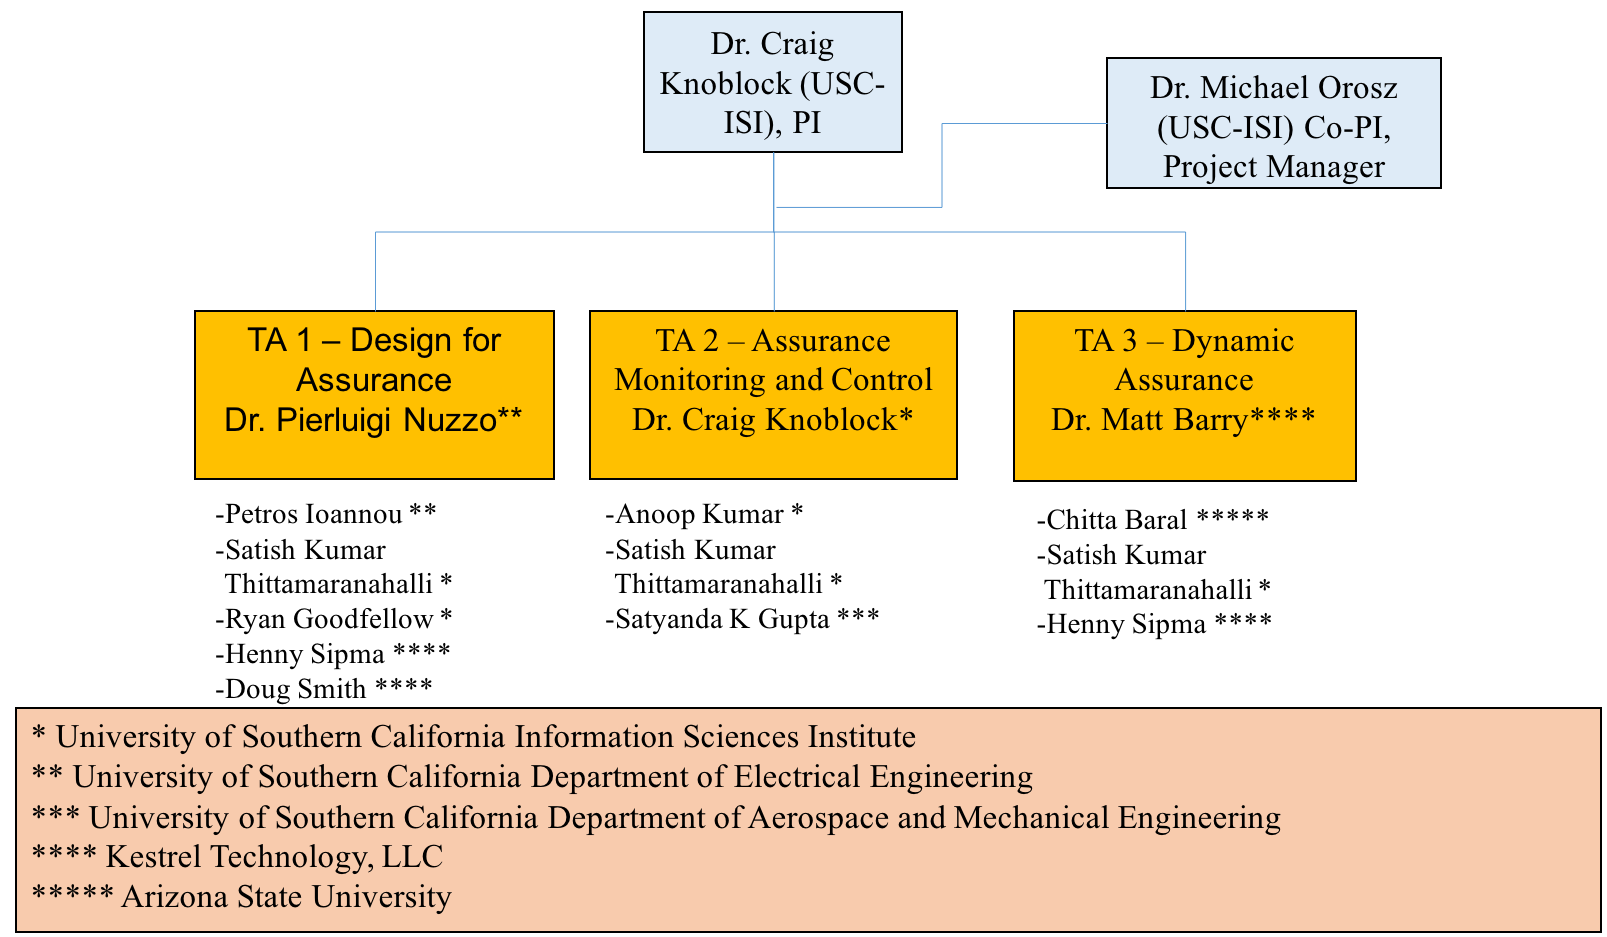
\includegraphics[width=6.0in]{./org-chart2.png}
\caption{\small Organization Chart}
\label{fig:org_chart}
\end{figure}

Coordination: To maximize collaboration and reduce risk to project failure from lack of communication and technical exchange, we plan to employ a wide variety of working styles and communication/coordination so that all can contribute.  At the core of our project will be regularly scheduled meetings bridging the diversely distributed team (Table~\ref{fig:Collaboration_Table}).  These meetings will address project status, identify challenges, implement risk mitigation strategies and participate in technology exchanges and system integration efforts (when appropriate)

\begin{table}[ht]
\caption{\small Project Meetings and Events}
  \centering
  {\footnotesize
\begin{tabular}{|m{3.15in}|m{3in}|} 
\hline
\textbf{Meeting} & \textbf{Frequency} 
\\\hline
Conference calls among investigators (discuss project status, address concerns and project risks) & Weekly
\\
\hline
Technical exchange and coordination meetings using Bluejeans or another videoconference technology & At least twice a month and more frequently as needed
  \\ 
\hline
Face-to-Face meetings (prior to P/I and demonstration meetings) & Every 3 to 6 months and more frequently (especially at the beginning of the project) as needed
 \\\cline{1-2}

\hline
\end{tabular}
}
\label{fig:Collaboration_Table}
\end{table}

\begin{table}[tbhp]
\caption{\small Key Project Team Member Responsibilities}
  \centering
  {\footnotesize
\begin{tabular}{| m{.75in} | m{3.9in}| m{1.5in}|} 
\hline
\textbf{Key Member} & \textbf{Responsibilities} & \textbf{Tasks} 
\\\hline
Dr.\ Craig Knoblock  & Principal Investigator responsible for project, leads TA 2 – Assurance Monitoring and Control.  Will lead the overall project and lead the TA2 team.  Served as the PI on many DARPA projects and has sucessfully led many large teams.    Effort on project:  25\% &
1.1.6, 1.2.2 1.2.3, 1.2.4, 1.3.4, 1.4.1, 
2.1.6, 2.2.2 2.2.3, 2.2.4, 2.3.4, 2.4.1, 
3.1.6, 3.2.2, 3.2.3, 3.2.4, 3.3.4, 3.4.1
\\
\hline
Dr.\ Michael Orosz & Co-Principal Investigator responsible managing the day-to-day operations of the project, assist technical teams as needed, coordinate with TA4 teams.    Has led many large complex multi-disciplined/multi-organizational projects in academic and industry environments.  Effort on project: 50\%
& 1.1.6, 2.1.6, 3.1.6, 1.4.1, 2.4.1, 3.4.1
  \\ 
\hline
Dr.\ Pierluigi Nuzzo 
& 
Co-Principal Investigator.  Leads the TA 1 - Design for Assurance team and conducts research on the formal methods for the design of the TA1 system.  Research experience on methodologies and tools for the design of cyber-physical systems; contracts, interfaces, and compositional methods for embedded system design; the application of automated formal methods and optimization theory to problems in embedded and cyber-physical systems.  Effort on project: 2 months/year (16.6\%)
& 
1.1.1, 2.1.1, 3.1.1 \\
\hline
Dr.\ Matthew Barry
& 
Key personnel.  Leads the TA 3 – Dynamic Assurance.   He will conduct the research on the dynamic assurance case language editors and parsers, the run-time system, and system integrations. Effort on project:  66\%
& 
1.3.2, 2.3.2, 3.3.2\\
\hline
Dr.\ Chitta Baral
& 
Key personnel responsible for learning assurance rules, supporting assurance rules with uncertainty and improving solver speed.  Expertise on ASP solvers, which will be used to reason about the assurance cases. Effort on project: 20\%
& 
1.3.1, 2.3.1, 3.3.1 \\
\hline
Dr.\ Doug Smith 
& 
Key personnel will support formal methods aspects of TA1, and lead the effort on abstract refinement. Expertise in field of automated correct-by-construction program generation.    Effort on project: 40\%
& 
1.1.5, 2.1.5, 3.1.5 \\
\hline
Dr.\ Henny Sipma
& 
Key personnel who will support the program verification tasks under TA1.  Will lead the effort on program verification.   Effort on project:  45\%
& 
1.1.5, 2.1.5, 3.1.5, 1.3.2, 2.3.2, 3.3.2 \\
\hline
Dr.\ Petros Ioannou
& 
Key personnel responsible providing and extending the assurance test bed, which will be available at the start of the project for autonomous vehicles.   Effort on project: 1 month/year (8.3\%)
& 
1.1.2, 2.1.2 (optional), 3.1.2 (optional)
\\
\hline
Dr.\ Satyandra Kumar Gupta
& 
Key Personnel providing autonomous command and control expertise to the TA-2 team.   Will lead the research on safety aware learning on TA2.   Past research on physics-aware decision making to facilitate automation.  Effort on project: 1 month/year (8.3\%)
& 
1.2.1, 2.2.1, 3.2.1 \\
\hline
Dr.\ Anoop Kumar 
& 
Key personnel providing support to the TA 2 project team.  Will lead the research on monitoring \& control and detecting distribution shifts.  Effort on project: 50\%
& 
1.2.1, 1.2.2, 1.2.3, 1.2.4, 2.2.1, 2.2.2, 2.2.3, 2.2.4, 3.2.1, 3.2.2, 3.2.3, 3.2.4\\
\hline
Dr.\ Satish Thittamaranahalli
& 
Key personnel developing scalable algorithms for TA1, TA2, and TA3 project teams.  Has extensive experience on scalable algorithm design, machine learning, and constraint reasoning.  Effort on project: 50\%
& 
1.2.1, 1.2.2, 1.2.3, 1.2.4, 2.2.1, 2.2.2, 2.2.3, 2.2.4, 3.2.1, 3.2.2, 3.2.3, 3.2.4, 1.1.4, 2.1.4, 3.1.4 \\
\hline
Dr.\ Ryan Goodfellow
& 
Key personnel providing support to the TA-1 project. Will lead the research on simulation-based testing.  Has extensive experience on simulation-based testing.  Effort on project:  30\%
& 
1.1.3, 2.1.3, 3.1.3 \\

\cline{1-2}

\hline
\end{tabular}
}
\label{fig:Table_Mgmt}
\end{table}



\newpage
\section{Personnel, Qualifications and Commitment}

{\bf Dr.\ Craig Knoblock}, the PI on this effort, is a Research Professor of both Computer Science and Spatial Sciences at the University of Southern California (USC) and Director of the Intelligent Systems Division at the USC Information Sciences Institute.   He received his Ph.D. from Carnegie Mellon University in computer science. 
%His research focuses on techniques for describing, acquiring, and exploiting the semantics of data.  
In previous projects he has worked on developing  scalable approaches to execution monitoring, accurate detection of sensor failures, and   automatic modeling and reconstruction of sensors.  He has published more than 300 journal articles, book chapters, and conference papers on these topics.  Dr. Knoblock is a Fellow of the Association for the Advancement of Artificial Intelligence (AAAI), a Distinguished Scientist of the Association of Computing Machinery (ACM), a Senior Member of IEEE, past President and Trustee of the International Joint Conference on Artificial Intelligence.
%and winner of the 2014 Robert S. Engelmore Award.  

{\bf Dr.\ Michael Orosz}, a Co-PI on this effort, is a Research Associate Professor of Civil and Environmental Engineering at the University of Southern California (USC) and Research Director of the Decision Systems Group at the USC Information Sciences Institute.  Dr. Orosz has over 30 years’ experience in commercial and government software development, basic and applied research, project management, academic research and has developed and deployed several commercially successful products.  His research interests are in machine learning and decision analytics as applied to intelligence analysis and autonomous command and control such as smart building controls.    Dr. Orosz has extensive experience in managing large complex multi-disciplined/multi-teamed research projects. %funded by DARPA, DHS, DoD, DoE, Industry, NASA, NRO, NSA and ONR.   
He received his Ph.D. in computer science from the University of California, Los Angeles.

{\bf Dr.\ Pierluigi Nuzzo}, a Co-PI on this project, is an Assistant Professor in the Department of Electrical Engineering at the University of Southern California. He received the Ph.D. in Electrical Engineering and Computer Sciences from the University of California at Berkeley. 
%in 2015, and the Laurea degree (MS) in electrical engineering (summa cum laude) from the University of Pisa, Italy, and the Sant'Anna School of Advanced Studies, Pisa, Italy.
%
%He has four years of research experience in analog and mixed signal circuit design as a researcher at IMEC, Leuven, Belgium, and over 10 years experience in design methodologies and tools for mixed-signal integrated circuits and cyber-physical systems, as a researcher at the University of Pisa, IMEC, UC Berkeley, and USC. 
His research interests
include: methodologies and tools for cyber-physical system and mixed-signal
system design; contracts, interfaces and compositional methods for embedded
system design; the application of formal methods and optimization theory to problems in embedded and cyber-physical systems and electronic design automation. 
%
Prof. Nuzzo received %First Place in the operational category and Best Overall
%Submission in the 2006 DAC/ISSCC Design Competition, 
a Marie Curie Fellowship
from the European Union in 2006, 
the University of California at Berkeley EECS
departmental fellowship in 2008, 
%the University of California at Berkeley Outstanding Graduate Student Instructor Award in 2013, 
the IBM Ph.D.
Fellowship in 2012 and 2014, 
%the Best Paper Award from the International Conference on Cyber-Physical Systems (ICCPS) in 2016, 
and the David J.~Sakrison Memorial Prize in 2016 for his doctoral research. 
%He is an author of 1 patent and over 60 publications.

{\bf Dr.\ Satyandra K. Gupta} is Smith International Professor in the Department of Aerospace and Mechanical Engineering at the University of Southern California. %Prior to joining the University of Southern California, he was a Professor in the Department of Mechanical Engineering and the Institute for Systems Research at the University of Maryland. He was the founding director of the Maryland Robotics Center and the Advanced Manufacturing Laboratory at the University of Maryland. 
He served as a program director for the National Robotics Initiative at the National Science Foundation from September 2012 to September 2014.  Dr. Gupta's interest is in the area of physics-aware decision making to facilitate automation. He has published more than 300 technical articles. He is a fellow of the American Society of Mechanical Engineers (ASME) and editor of ASME Journal of Computing and Information Science in Engineering. Dr. Gupta has received the Young Investigator Award from the Office of Naval Research in 2000, CAREER Award from the National Science Foundation in 2001, Presidential Early Career Award for Scientists and Engineers (PECASE) in 2001, Invention of the Year Award at the University of Maryland in 2007, Kos Ishii-Toshiba Award from ASME in 2011, and Excellence in Research Award from ASME in 2013.%, and Distinguished Alumnus Award from Indian Institute of Technology, Roorkee in 2014. %He has also received seven best paper awards at conferences.

{\bf Ryan Goodfellow} is a computer scientist at ISI working in combined cyber physical simulation and emulation platform development. His formal background is in simulation algorithms and modeling techniques using differential-algebraic equations (DAE). He has applied this knowledge in the CPS space by integrating DAE modeling languages and simulation engines with network testbeds to create comprehensive scientific experimentation platforms for cyber-physical systems. These experimentation platforms have been used in the power grid research space. %Ryan is a lead developer on the Deter network testbed, with a strong background in networked and distributed systems engineering. %He is also a combat veteran, serving as a non-commissioned officer and SIGINT team lead for a multi-functional intelligence team in Afghanistan.

{\bf Dr.\ Petros Ioannou} is a Professor in the Department of Electrical Engineering, Director of the Center for Advanced Transportation Technologies and Associate Director for Research for the DOT supported University Transportation Center at USC. He received his MS and PhD from the University of Illinois at Urbana Champaign in Mechanical and Electrical Engineering, respectively. His research interests are in robust adaptive control, vehicle dynamics and control, human factors and safety, automated vehicles, nonlinear systems and Intelligent transportation Systems.  He received the 2016 IEEE Transportation Technologies field award and the 2016 IEEE Control system society Transition to Practice Award. He is a Fellow of IEEE, IFAC and IET and author/coauthor of 8 books and over 400 papers.

{\bf Dr.\ Matthew Barry} will serve as lead for the TA3 tasks. %He will implement the dynamic assurance case language editors and parsers, the run-time system, and system integrations.  He will implement the assurance case arguments and the API for updating argument structure and content.  
Dr. Barry currently is CEO at Kestrel Technology LLC, and previously spent 20 years in NASA space mission operations at the Jet Propulsion Lab and Johnson Space Center.  At NASA Headquarters he led the introduction of dependability case requirements and plans for flight computing systems in upcoming manned space exploration missions, as well as the development of Agency-level software-related safety-critical control system requirements.  He recently served as a Principal Investigator on DHS/Cyber S\&T STAMP (Static Tool Analysis Modernization Program), DARPA CSFV (Crowd Sourced Formal Verification), three NASA Aeronautics R\&D projects, and the AFRL-sponsored Static Analysis of Numerical Algorithms project.  Dr. Barry earned BSME, MS, and PhD degrees in mechanical engineering, and an MBA degree, from Rice University.  

{\bf Dr.\ Henny Sipma} will support the program verification tasks under TA1.  %She is the key person behind the company's {\em KT Advance\/} and {\em KT Transferal\/} static analysis products, and the designer and programmer of the company's core {\em CodeHawk\/} abstract interpretation engine. 
Dr. Sipma currently is the CTO at Kestrel Technology LLC.  She has spent the past 10 years with Kestrel Technology as a static analysis expert; previously developed and taught static analysis techniques as senior research associate at Stanford University for eight years; and developed industrial process controls as an senior systems analyst at Shell.  She has been Principal Investigator or company lead on several recent R\&D projects for Federal agencies, including two projects under the IARPA STONESOUP (Securely Taking On New Executable Software of Uncertain Provenance) program; the DHS Cyber S\&T Gold Standard project; and the DARPA-sponsored STAC (Space-Time Analysis for Cybersecurity) and MUSE (Mining and Understanding Software Enclaves) programs.  Dr. Sipma earned 
%a BS degree in chemistry and an MS degree in chemical engineering at the University of Groningen in The Netherlands, and 
MS and PhD degrees in computer science from Stanford University.  

{\bf Dr.\ Douglas R.\ Smith} will support formal methods aspects of TA1, including the enforcement of safety properties and the generation of monitors.  He is President of Kestrel Technology LLC and Principal Scientist at Kestrel Institute.  He is a Fellow of the American Association of Artificial Intelligence (AAAI) and an ASE Fellow (Automated Software Engineering).  From 1986 to 2000, he taught an advanced graduate course on correct-by-construction software development at Stanford.  
%Dr. Smith has led the development of a series of software synthesis systems, including KIDS (Kestrel Interactive Development System), Specware, Designware, and Planware. 
%Applications domains have included a variety of complex high-performance planners and schedulers for the US Air Force.  He leads current projects on the generation of air mission plans and cyberoperations.  
Other recent projects focused on automated policy enforcement \cite{SmithD0703,SmithD08}, synthesis of secure network protocol codes, and the synthesis of high-performance constraint-solvers\cite{SmithD08c,SmithD13}.  Dr. Smith has over 30 years experience in the field of automated correct-by-construction program generation and has published over 100 papers. He has one patent.  He received the Ph.D. in Computer Science from Duke University% in 1979.  

{\bf Dr. Chitta Baral} is a Professor in the Department of Computer Science and Engineering at Arizona State University. He will support the TA3 efforts on Learning assurance rules, supporting assurance rules with uncertainty and improving solver speed. Dr. Baral has expertise in various aspects of autonomy and Artificial Intelligence. 
He wrote the first book on answer set programming (published by Cambridge University Press) the formal language behind our assurance rules. Some of his other works relevant to this proposal are: goal specification for autonomous systems, automatic construction of control rules for autonomous systems that satisfy given goals, combining machine learning with reasoning in various contexts, including image understanding. %He is the President of KR Inc. He is an associate editor of AIJ and has been an associate editor of JAIR.

{\bf Dr.\ Satish Kumar Thittamaranahalli (T. K. Satish Kumar)} leads the Collaboratory for Algorithmic Techniques and Artificial Intelligence (CATAI) at USC's Information Sciences Institute. He has published over 60 papers on numerous topics in Artificial Intelligence spanning such diverse areas as Constraint Reasoning, Planning and Scheduling, Probabilistic Reasoning, Robotics, Combinatorial Optimization, Approximation and Randomization, Heuristic Search, Model-Based Reasoning, Knowledge Representation and Spatio-Temporal Reasoning. %He %has served on the Program Committees of many international conferences in Artificial Intelligence
He and is a winner of the 2016 Best Robotics Paper Award and the 2005 Best Student Paper Award from the International Conference on Automated Planning and Scheduling. 
Dr. Kumar received his PhD in Computer Science from Stanford University. %In the past, he has also been a Visiting Student at the NASA Ames Research Center, a Postdoctoral Research Scholar at the University of California, Berkeley, a Research Scientist at the Institute for Human and Machine Cognition, a Visiting Assistant Professor at the University of West Florida, and a Senior Research and Development Scientist at Mission Critical Technologies.

\textbf{Dr.\ Anoop Kumar} is a senior computer scientist at USC ISI and has broad expertise in machine learning, statistical modeling, and software engineering.  Dr.\ Kumar is the technical lead on the DARPA RSPACE program and has played a vital role in developing a system that fuses air operations data from multiple sources, maintains world state, and issues warnings. Previously, he led the research and development of the BBN’s election forecasting system for the IARPA OSI program. %Dr.\ Kumar played a significant role in the DARPA DEFT program by developing a model to support integration of output from multiple NLP algorithms. He has contributed at the development to management levels on government research contracts and commercial projects. 
Dr.\ Kumar helped design and develop BBN's commercially available, hosted speech and medical transcription services offering. 

\begin{table}[!tbh]
\begin{footnotesize}
\vspace{-0.1in}

\begin{tabular}{lll}
\begin{tabular}[t]{|l|@{}c@{}|@{}c@{}|@{}c@{}|@{}c@{}|} \hline
Project & Status & \multicolumn{3}{ c| }{Hours} \\ \cline{3-5}
& & P1 & P2 & P3 \\ \hline



\multicolumn{5}{ |c| }{ \textbf{Craig Knoblock} } \\ \cline{1-5}
Safeguard & Pro & 770 & 641 & 641 \\ \cline{1-5}
ELICIT & Cur & 308 & 256 & 120 \\ \cline{1-5}
WTNIC & Cur & 11 & 0 & 0 \\ \cline{1-5}
EFFECT & Cur & 641 & 107 & 0 \\ \cline{1-5}
LinkedMaps & Cur & 203 & 25 & 0 \\ \cline{1-5}
PRINCESS & Cur & 608 & 96 & 0 \\ \cline{1-5}
SCHARP & Cur & 481 & 54 & 0 \\ \cline{1-5}
MINT & Pen & 650 & 534 & 285 \\ \cline{1-5}

\multicolumn{5}{ |c| }{ \textbf{Michael Orosz} } \\ \cline{1-5}
Safeguard & Pro & 1560 & 1300 & 1300  \\ \cline{1-5}
SMC/SY & Cur & 1803 & 0 & 0  \\ \cline{1-5}

\multicolumn{5}{ |c| }{ \textbf{Matthew Barry} } \\ \cline{1-5}
Safeguard & Pro & 2078 & 1690 & 1554 \\ \cline{1-5}
Starlite & Cur & 1840 & 1692 & 0 \\ \cline{1-5}



\multicolumn{5}{ |c| }{ \textbf{Anoop Kumar} } \\ \cline{1-5}
Safeguard & Pro & 1560 & 1300 & 1300 \\ \cline{1-5}

\end{tabular}
&
\begin{tabular}[t]{|l|@{}c@{}|@{}c@{}|@{}c@{}|@{}c@{}|} \hline
Project & Status & \multicolumn{3}{ c| }{Hours} \\ \cline{3-5}
& & P1 & P2 & P3 \\ \hline

\multicolumn{5}{ |c| }{ \textbf{Pierluigi Nuzzo} } \\ \cline{1-5}
Safeguard & Pro & 520 & 433 & 433  \\ \cline{1-5}
Mirage & Cur & 433 & 0 & 0  \\ \cline{1-5}

\multicolumn{5}{ |c| }{ \textbf{Satyandra Gupta} } \\ \cline{1-5}
Safeguard & Pro & 260 & 217 & 217 \\ \cline{1-5}
Human   & Cur & 22 & 0 & 0 \\ \cline{1-5}
Vehicles & Cur & 36 & 0 & 0 \\ \cline{1-5}
Robot & Cur & 116 & 0 & 0 \\ \cline{1-5}
Assembly & Cur & 33 & 0 & 0 \\ \cline{1-5}
Solar & Cur & 4 & 0 & 0 \\ \cline{1-5}

\multicolumn{5}{ |c| }{ \textbf{Petros Ioannou} } \\ \cline{1-5}
Safeguard & Pro & 260 & 217 & 217 \\ \cline{1-5}
CPS & Cur & 130 & 0 & 0 \\ \cline{1-5}

\multicolumn{5}{ |c| }{ \textbf{Ryan Goodfellow} } \\ \cline{1-5}
Safeguard & Pro & 936 & 780 & 780 \\ \cline{1-5}
STEAM & Cur & 416 & 0 & 0 \\ \cline{1-5}


\end{tabular}
&
\begin{tabular}[t]{|l|@{}c@{}|@{}c@{}|@{}c@{}|@{}c@{}|} \hline
Project & Status & \multicolumn{3}{ c| }{Hours} \\ \cline{3-5}
& & P1 & P2 & P3 \\ \hline

\multicolumn{5}{ |c| }{ \textbf{Chitta Baral} } \\ \cline{1-5}
Safeguard & Pro & 659 & 485 & 485 \\ \cline{1-5}
PostdocBP & Cur & 176 & 0 & 0 \\ \cline{1-5}
Languages & Pen & 528 & 264 & 264 \\ \cline{1-5}
CAREER & Pen & 88 & 44 & 44 \\ \cline{1-5}
CHS & Pen & 510 & 255 & 0 \\ \cline{1-5}

\multicolumn{5}{ |c| }{ \textbf{Doug Smith} } \\ \cline{1-5}
Safeguard & Pro & 1222 & 984 & 840 \\ \cline{1-5}
RSPACE & Cur & 342 & 0 & 0 \\ 
\cline{1-5}
PLANX & Cur & 154 & 0 & 0 \\ 
\cline{1-5}
HACCS & Pen & 923 & 769 & 769 \\ 
\cline{1-5}

\multicolumn{5}{ |c| }{ \textbf{Henny Sipma} } \\ \cline{1-5}
Safeguard & Pro & 1372 & 962 & 840 \\ \cline{1-5}
STAC & Cur & 797 & 0 & 0 \\ \cline{1-5}

\multicolumn{5}{ |c| }{ \textbf{Satish Thittamaranahalli} } \\ \cline{1-5}
Safeguard & Pro & 1560 & 1300 & 1300 \\ \cline{1-5}
MapF & Cur & 103 & 103 & 0 \\ \cline{1-5}

\end{tabular}
\end{tabular}

\end{footnotesize}
\caption{Individual commitments of key personnel}
\label{tab:Commitments}
\vspace{-0.2in}
\end{table}

\clearpage
\newpage
\section{Capabilities}


%\subsection{University of Southern California}
USC has strengths in number of areas that are closely related to the proposed work:
\begin{itemize}[itemsep=0pt,leftmargin=*]
\item Dr.\ Nuzzo 
%has over 10-year research experience in embedded system design, from mixed-signal chip design (analog-to-digital converters, frequency synthesizers, software-defined radio), to methodologies and tools for mixed-signal integrated circuits and Cyber-Physical Systems (CPSs), and the application of formal methods and optimization theory to problems in embedded and cyber-physical systems and electronic design automation.  
%His doctoral work 
has done extensive research on contracts and compositional methods for heterogeneous system design and design space exploration, with application to aircraft electric power systems and environmental control systems. His work has helped transition rigorous system design foundations, innovative design methodologies, and new systems engineering paradigms to industry (IBM, United Technologies). 
\item Dr.\ Satyandra K. Gupta has worked on autonomous surface vehicles, autonomous ground vehicles for operation on rugged terrains, and autonomous flapping wing aerial vehicles.   His group has developed a hierarchal decision making approach for realizing autonomous systems. 
%This approach combines task planning and assignment, deliberative trajectory planning, reactive collision avoidance behaviors, and trajectory tracking control layers. 
His group has also developed new methods for learning reactive behaviors in adversarial environments and COLREGS compliant trajectory planning. \item Dr.\ Knoblock has developed methods that learn the relationships between sensors to both identify failures and changes in sensor and reconstruct those sensors, providing estimates of the accuracy of the reconstructed sensors.  
\item Ryan Goodfellow has extensive experience in simulation based testing through high-fidelity CPS testbed environment development and operation, using the Deter network testbed as the core which has supported several large scale government projects from a variety of agencies and thousands of users. %we have developed sophisticated CPS experiments under programs such as NFS RIPS, NIST SmartCities and the DHS Cybersecurity showcase.
\item Dr.\ Ioannou %helped  design and implement adaptive cruise control systems in collaboration with Ford Motor Company, which was commercialized four years before any other company. He 
worked on several DOT funded projects on automated vehicles and intelligent highway systems where he demonstrated his vehicle control designs for safety and performance on actual automated vehicles in test trucks and I-15 highway.
\item Drs.\ Knoblock, Kumar, and Thittamaranahalli have developed highly scalable approaches for monitoring message traffic to identify potential problems and issue warnings and alerts. 
\item Dr. Thittamaranahalli has developed state-of-the-art methods for efficiently solving large-scale search and optimization problems. %These techniques will be applicable in TA2 for safety-aware learning and planning, in TA2 for assurance monitoring and control, and in TA3 for dynamic assessment of assurance cases.

\end{itemize}
%\subsection{Kestrel Technology LLC}

Kestrel Technology's strength is in program analysis, specifically static analysis of both source and binary targets.  The company performs applied R\&D and product development for a variety of static analysis applications  pivoting primarily on the abstract interpretation technique.  The company recently initiated development of program analysis applications using logical equivalence techniques. As a provider of verification evidence in the form of mathematical proofs, the company also has expertise in the design and development of assurance case arguments for high-integrity systems using such evidence. %The company is engaged in a partnership with Wind River Systems to develop program analysis tools for its embedded system developers.  Many of Wind River's customers must develop their products under safety and certification standards, including those using safety cases.  

   

%\subsection{Arizona State University}
Chitta Baral at Arizona State University has developed various software to learn assurance rules and various ASP solvers, which he has made available as open-source.

Most of the software carried forward for implementation or derivation is open source.  The single exception is Kestrel Technology's {\it KT Advance\/} static analysis tool (TA1), in particular the abstract interpretation engine therein, which is company proprietary and is US EAR export-controlled.   
%Owing to mixed funding for the development of that technology 
We will continue to provide the Federal government a restricted use license for that particular item.

There are no specialized facilities, data, or GFE required for this effort. 

\include{sow}
\include{milestones}

% \section{Level of Effort by Task \textcolor{red}{[Mike/Lisa - 1 pages]}}

% \textcolor{blue}{
% \begin{itemize}
% \item Will be a separate spreadsheet
% \item
% \end{itemize}
% }

\include{appendix_a}

%\section{Appendix B \textcolor{red}{[No Page Count]}}

\section{References}
\bibliographystyle{acm} 
\bibliography{TA3/ta3,TA2/ta2,TA1/ta1}
\end{document}
%%\documentclass[a4paper]{article}
%\documentclass[12pt]{article}
\documentclass[12pt]{dod-blank}

%% Language and font encodings
\usepackage[english]{babel}
\usepackage[utf8x]{inputenc}
\usepackage[T1]{fontenc}

%% Sets page size and margins
%%\usepackage[a4paper,top=3cm,bottom=2cm,left=3cm,right=3cm,marginparwidth=1.75cm]{geometry}
%\usepackage[top=1in, bottom=1in, left=1in, right=1in]{geometry}



%% Useful packages
\usepackage{amsmath}
\usepackage{graphicx}
  \graphicspath{{.}{./image/}}
  \DeclareGraphicsExtensions{.png,.jpg} 
\usepackage[colorinlistoftodos]{todonotes}
\usepackage[colorlinks=true, allcolors=blue]{hyperref}
\usepackage{tabularx}
\usepackage{multirow}
\usepackage{tabulary}
\usepackage{float}
\usepackage{wrapfig}
\usepackage[export]{adjustbox}
\usepackage{comment}
\usepackage{tabularx}
\usepackage{multirow}
\usepackage{tabulary}
\usepackage{enumitem}

\usepackage{listings}
\usepackage{color}
\usepackage{array}
\usepackage{subcaption}
\usepackage{xcolor}




\renewcommand{\textfraction}{0}
\renewcommand{\topfraction}{1.0}
\renewcommand{\bottomfraction}{1.0}

\usepackage{longtable}
%% macros
\newif\iffinal
\finaltrue
\iffinal
  
    \newcommand\baareq[1]{}
    \newcommand\baades[1]{}
 
 
\else
    \definecolor{darkgreen}{rgb}{0,0.4,0}
    \definecolor{darkcyan}{rgb}{0,0.4,0.4}
    \definecolor{darkblue}{rgb}{0,0,0.5}
    
    \newcommand\baareq[1]{{\color{darkcyan}[\textbf{Requirement:} #1]}}
    \newcommand\baades[1]{{\color{darkcyan}[\textbf{Description:} #1]}}
 
\fi




\def\naive{na\"{\i}ve}



\lstset{ 
  backgroundcolor=\color{white},   % choose the background color; you must add \usepackage{color} or \usepackage{xcolor}
  basicstyle=\footnotesize\ttfamily,            % the size of the fonts that are used for the code
  breakatwhitespace=false,         % sets if automatic breaks should only happen at whitespace
  breaklines=true,                 % sets automatic line breaking
  captionpos=b,                    % sets the caption-position to bottom
  commentstyle=\color{mygreen},    % comment style
  % deletekeywords={...},            % if you want to delete keywords from the given language
  escapeinside={\%*}{*)},          % if you want to add LaTeX within your code
  extendedchars=true,              % lets you use non-ASCII characters; for 8-bits encodings only, does not work with UTF-8
  frame=single,	                   % adds a frame around the code
  keepspaces=false,                 % keeps spaces in text, useful for keeping indentation of code (possibly needs columns=flexible)
  keywordstyle=\color{blue}\bfseries\underbar,       % keyword style
  language=Prolog,                 % the language of the code
  % morekeywords={if,and},        % if you want to add more keywords to the set
  numbers=none,                    % where to put the line-numbers; possible values are (none, left, right)
  numbersep=5pt,                   % how far the line-numbers are from the code
  numberstyle=\tiny\color{mygray}, % the style that is used for the line-numbers
  rulecolor=\color{black},         % if not set, the frame-color may be changed on line-breaks within not-black text
  showspaces=false,                % show spaces everywhere adding particular underscores; it overrides 'showstringspaces'
  showstringspaces=false,          % underline spaces within strings only
  showtabs=false,                  % show tabs within strings adding particular underscores
  stepnumber=2,                    % the step between two line-numbers. If it's 1, each line will be numbered
  stringstyle=\color{mymauve},     % string literal style
  tabsize=2,	                   % sets default tabsize to 2 spaces
  title=\lstname                   % show the filename of files included with \lstinputlisting; also try caption instead of title
}

% apply trick for additional keywords for our AC DSL
\lstset{
	emph={for, if, and, or},
    emphstyle={\color{blue}\bfseries\underbar}
}




\title{DARPA Assured Autonomy}
\author{Technical Volume- \textcolor{red}{Thirty-Eight (38) pages max}}

\begin{document}
\pagenumbering{roman}
\include{cover}

\newpage
\section{Table of Contents}
\tableofcontents

\newpage
\pagenumbering{arabic}
\section{Executive Summary}
As we rapidly move into a world where machine learning plays a central role in realizing autonomous systems, it is becoming increasingly important to develop techniques that assure that these systems will operate safely and perform as expected. Current approaches are limited to providing assurance for systems with limited or no  learning capabilities. In this context, DARPA's Assured Autonomy BAA seeks to \emph{develop rigorous design and analysis technologies for continual assurance of learning-enabled autonomous systems}. USC in collaboration with Kestrel Technology and ASU is pleased to submit a comprehensive TA1, TA2, and TA3 proposal entitled \emph{``Assured Autonomy for Learning Enabled Vehicles (Safeguard).''} We plan to provide an end-to-end solution to support autonomous systems with learning-enabled components, ranging from design technologies for assurance, to assurance monitoring and control techniques, to representation and online evaluation of assurance cases. We have assembled a strong team of experts that cover the range of technologies that are required to create such an end-to-end system. If successful, the project will provide the technologies for building the next-generation of learning-enabled autonomous systems.  The entire project will take four years and cost \textcolor{red}{\$??}, with an initial version completed at the end of Phase I and successive versions with additional capabilities and improved scalability at the end of Phase II and Phase III.  

In the remainder of this section, we first introduce an  unmanned surface vehicle scenario that will be used throughout the proposal to describe the approach.  Next, we describe our approach to design, monitoring, and dynamic assurance. Finally, we introduce the team involved in the project. 

\textbf{Motivating Scenario.} Consider an autonomous unmanned surface vehicle (USV) guarding a valuable asset in the ocean when an unknown vehicle  approaches the security perimeter, under challenging weather conditions. In this scenario, the USV is required to approach the intruding vehicle, issue a warning signal, and escort it to a safe distance from the controlled area. However, as the USV has no a priori knowledge of its external environment behaviors (e.g., water depth, waves, wind, current, visibility), pre-computing a feasible trajectory, let alone optimal, becomes a non-trivial problem. For trajectory planning, the USV must continuously perform the following tasks:
\begin{itemize}[itemsep=0pt,leftmargin=*]
 \item Sense the current state of the surrounding environment (e.g., water depth, waves, wind, current, visibility) and estimate its own maneuverability constraints (e.g., braking distance, available acceleration, maximum velocity, turning radius, turning rate, safety distance) based on the state of the environment;      
\item Sense the static obstacles in the sensor range and generate a traversability map;
\item Sense the moving obstacles and classify them;   
\item Predict future trajectories of moving obstacles; 
\item Determine if any of the COLREGS \cite{commandant1999international} rules will be in effect with respect to one or more of the nearby vessels and identify the vessels with the right of way.    
\end{itemize}
The above information will be used by the trajectory planner to compute an initial trajectory, which will be continuously refined as the USV gathers additional information.
% It is not possible for the USV to be tested in every possible environment. 
The USV will use learning enabled components to take  decisions as it encounters new situations, such as  
\begin{itemize}[itemsep=0pt,leftmargin=*]
\item Classifiers to identify moving obstacles based on physical appearance and motion signatures,
\item Algorithms to estimate the sensor capabilities in adverse weather conditions,   
\item Algorithms to accurately estimate uncertainty in the environment, 
\item Classifiers to generate traversability maps,
\item Prediction of external vessel behaviors based on motion histories, 
\item Reinforcement learning  to ensure COLREGS compliance of maneuvers,  
\item Algorithms to learning pursuit behaviors.  
\end{itemize}
Learning enabled components will interact with each other in complex ways, where a misclassification error in one component may eventually compromise the entire mission.   
% We will need to make sure that each learning enabled components has a run-time monitor that will ensure that the assumptions made by the learning-enabled component remain valid and prevent erroneous learning. 
% For example, if the vehicle is exhibiting significant error in trajectory tracking, then simply downgrading the trajectory tracking error value may not be a good option.  The failure of prediction of trajectory tracking error might be due to the presence of a significant wake caused by a nearby vessel. The presence of the nearby vessel can be used to explain the degradation in trajectory tracking performance. As the vessel moves away, we can expect the trajectory tracking performance to return to the predicted level.  
While exhaustive validation of learning-enabled cyber-physical systems (LE-CPSs) is a prohibitive task~\cite{Kalra16},
their complexity, heterogeneity, and highly dynamic nature
make it challenging to even leverage existing model-based development techniques to effectively assess system correctness 
% dependability, 
at design time or enforce it at runtime.

\textbf{Design for Assurance.} Safeguard uses a platform-based design approach~\cite{Nuzzo15b} to organize the design process for a LE-CPS and to build assurance cases. Composite models are developed at several levels of abstraction,
from top-level system requirements and safety constraints down to the
implementation level.  Intermediate levels add detail to the levels
above.  The different levels are connected by refinement mappings that
allow properties established at one level to be preserved at the next
level (see Figures~\ref{fig:methodology} and~\ref{fig:assurance}).

Contracts are used to formally specify components and composite models
in terms of (1) Assumptions -- the assumed behaviors of the
environment and the behaviors of other components, and (2) Guarantees
-- the behavior properties that a model guarantees if it operates in a
context that satisfies its assumptions.  A calculus of contracts
allows horizontal composition of contracts to generate contracts for
composite models.  Vertical contracts are used to specify the mapping
or refinement relation between models at different levels of
abstraction.  The system design process starts with a high-level
contract that expresses overall system assumptions and requirements.
Subsequent levels express models with increasing detail until the
lowest level expresses the system in terms of hardware components and
their software controllers.

The assurance case for a CPS arises from the horizontal and vertical
structure of the design in several ways.  The components used within a
particular level are either (1) synthesized using
correct-by-construction design tools together with proofs, (2) derived
statically or dynamically using safety-aware machine-learning
techniques, (3) written manually and verified by analysis tools, or
(4) written manually and validated by extensive testing.  The
assurance case for the whole reflects its compositional structure.  We
anticipate that well-specified contracts together with the calculus of
contracts will eliminate well-known problems with unexpected emergent
behaviors in CPS systems.

The assurance case for the lowest-layer design arises from both the
intra-level assurance and from properties and their proofs that are
preserved under the refinement mapping from the top-level
requirements.  The refinement mappings between model layers will be
constructed using a variety of techniques.  A contract at an abstract
level can be mapped to a component or refined contract by (1)
retrieval of pre-verified components from a platform library, (2)
synthesis using correct-by-construction design and optimization tools,
or (3) manual coding to satisfy a contract.  The mapping of a
composite model will be composed from the mappings of its constituent
components or contracts.  When a composite model cannot be mapped
compositionally to the next level, it will be generated using
correct-by-construction design and optimization tools.

\textbf{Assurance Monitoring and Control.}
We provide an integrated framework for safety-aware learning, assurance monitoring and control, detecting distribution shifts. Three major components offer an efficient TA2 architecture as well as interfaces with TA1 and TA3, that is, (a) safety-aware learning and planning, (b) assurance monitors for guarding architectural and safety constraints; and (c) distribution shift detection.

We will develop a new learning-enabled online decision-making framework that allows opportunistically composing a sequence of actions (maneuvers) to reduce uncertainty in the system capability model without suspending the progress toward the mission goals or compromising safety. Each candidate action is evaluated based on three criteria: (1) the risk of violating a safety constraint using the current uncertainties in the parameter estimates; (2) its relevance to the mission goals; (3)  its expected information gain, i.e., reduction in uncertainty, with respect to the parameter estimates. These evaluations are combined to produce a cumulative mission utility value for each action that drives our learning-enabled decision-making framework. The problem of generating and evaluating sequences of actions can be posed in several way. For example, it can be solved using a branch-and-bound search method like Anytime A*, or formulated with the finite-horizon Markov Decision Process (MDP) framework. We will develop new scalable search strategies to solve this problem efficiently, by potentially evaluating a recent method developed at USC, called FastMap, that can significantly improve the execution time. 

We will develop monitors for architectural and safety constraints. 
% While these constraints can be checked over and over again as sensor information flow in, this naive strategy accounts for a lot of computational overhead. 
To achieve scalability and decrease the overhead, we propose the application of a technique that we currently use in DARPA's RSPACE program, which leverages a physical model of the vehicles dynamics and its interactions with the environment to efficiently determine the readout frequency. We propose two  extensions of this basic idea. First, we will use the theory of Variable Elimination to prioritize which variables to monitor, e.g., controllable, versus uncontrollable, adversarially controlled, or unobservable variables. Second, we invoke the dynamic assessment of assurance cases only when needed. This  decreases the number of times dynamic assessment of assurance cases is initiated as well as the communication bandwidth between the TA2 and TA3 components.

Finally, we will identify a distribution shift by combining statistical and machine learning techniques to differentiate between environmental and sensor changes. We will exploit a categorization of the shifts based on their cause and duration as well as extend our earlier work on detecting and mitigating sensor failures for all types of monitored variables.  

\textbf{Dynamic Assurance:} The Safeguard {\em design for assurance\/} activity takes a systems-theoretic stance toward safety.  Consequently, it presumes that safety is an emergent property of the system, and that hazards can present themselves through unintended interactions and performance violations in addition to causal events such as component failures.  Our design approach includes consideration of intent as well as hazard analysis and mitigation.  The artifacts from these activities populate contracts and assumptions for the dynamic assurance case.  
We thus build safety into the product by working at a systems-level viewpoint, using lexicon and design patterns familiar to both hardware and software engineers; safety is an emergent property of the system, not an afterthought.  
As system behavior evolves during runtime owing to learning, threats, degradation, or some other factor, the dynamic assurance case identifies whether the safety constraints continue to be satisfied.  If not, it provides notifications or issues recovery instructions directly from a lookup table.

Our implementation of the dynamic assurance case employs a declarative knowledge base inference engine and a domain-specific language tailored to our approach.  We have used them successfully for assurance case tool sets and arguments, and will extend them to reason about uncertainty and learning.  Our approach to achieve scalability is to specialize solvers toward modularity and to take advantage of domain knowledge.  Specifically, we will develop answer set programming techniques for context-dependent learning for reasoning about the learning-enabled components as well as learning assurance rules.  We will develop new formalisms for uncertainty to include causality, using weights for computing probabilities, and probabilistic non-monotonicity.  To achieve scaling objectives we will implement specializations using modularity, weighted CSPs, and message passing. 

% The system safety constraints revealed from that design become the key elements of our dynamic assurance case.  Our verification tools ensure the constraints are relevant, identifiable, and their implementation and effect observable.  

\textbf{Team.} We have assembled a team that is exceptionally well-qualified to build the proposed Safeguard system.  The team will be led by Dr.\ Craig Knoblock, the Principal Investigator for the effort, who currently leads the Intelligent Systems Division at the Information Sciences Institute.  He has led many large DARPA and IARPA projects over the years and has a strong track record in conducting leading edge research and then transitioning the technology to commercial use.  He will be supported by Dr.\ Michael Orosz as the Project Manager, who also has  experience in managing large research projects and on autonomous systems.  The TA1 team will be led by Dr.\ Pierluigi Nuzzo, who is an expert in embedded system design methodologies and the  application of formal methods to cyber-physical systems.  The TA1 team also includes Dr.\ Doug Smith, who has spent many years working on scalable correct-by-construction techniques and Dr.\ Henny Sipma, who has significant experience in applying program verification methods to real-world problems.  The TA1 team also includes Ryan Goodfellow, who has done a large amount of work on simulation-based testing.  The TA2 team will be led by Dr.\ Knoblock who has worked on topics related to both monitoring and detecting distribution changes.  He will be supported by Dr.\ Satyandra Gupta, who is an expert on autonomous surface vehicles as well as on safety-aware learning. He will also be supported by Drs.\ Anoop Kumar and Satish Thittamaranahalli, who have also previously worked on efficient methods for execution monitoring.  The TA3 team will be lead by Dr.\ Matthew Barry, who has experience in creating the technologies for assurance cases.  He will be supported by Dr.\ Chitta Baral, who is an expert on ASP solvers and by Dr.\ Thittamaranahalli who is an expert on SAT solvers, both of which will be applied to provide scalable assurance case reasoning.  Finally, Dr.\ Petros Ioannou, who is an expert on control systems for autonomous vehicles will provide an autonomous vehicle platform, which will form the focus of our work until the TA4 teams provide additional vehicle platforms for development.  

\newpage
\section{Innovative Claims and Deliverables}

In this project we will develop and build an end-to-end system for assured autonomy.  This section describes the key innovations by technical area and then the overall deliverables of the project.

\paragraph{Design for Assurance}

\begin{itemize}[itemsep=0pt,leftmargin=*]
\item We address the LE-CPS design challenges via a holistic approach that can contextually generate design artifacts and assurance cases. We develop a compositional, contract-based modeling framework, methods, and tools to support the design process from system-level requirement capture,  formalization, and analysis, to the generation, testing, and continual monitoring of software and hardware artifacts in feedback loop with a physical process.

\item We develop compositional abstractions and interfaces (vertical contracts) that can  bridge heterogeneous formalisms and heterogeneous decomposition architectures to make system analysis and synthesis tractable, consistently combine different verification and synthesis methods at design time, and provide seamless support for dynamic assurance at run time. %We aim to quantitatively capture the confidence in the satisfaction of requirements under uncertain or unknown conditions, and resilience properties of  systems at different abstraction levels, to enable trade-off evaluation between resilience, performance, and cost.

\item We develop a unifying framework and efficient algorithms to reason about the combination of discrete and continuous dynamics and constraints in the presence of uncertainties in LE-CPS using a satisfiability modulo convex approach~\cite{Shoukry2017} for contract-based system verification and scalable trajectory planning.  

\item We provide an environment for high-fidelity CPS testing, in which production-ready software, e.g.,  safety-critical learning and control, may be deployed and tested 
% by extending the Cypress testbed environment \cite{Goodfellow2015Cypress:Systems} 
with time dilation facilities, so that it synchronizes with a physical simulation that is not necessarily running in real time, while still having the perception of real time.

\item We 
% These facilities allow a cyber system to be  
propose an approach for unanticipated behavior space identification and test coverage maximization which leverages results from the theory of differential algebraic equation (DAE)~\cite{Berger2013ControllabilitySurvey,Ilchmann2005ATheory,BergerOnSystems,Lamour2013} 
to prune the behavior search space and identify smaller regions of interest for efficient simulation-based testing. 
% We then compute the intersection of these two behavior spaces and restrict our simulation based testing search space to this subspace.
\end{itemize}

\paragraph{Assurance Monitoring and Control}

\begin{itemize}[itemsep=0pt,leftmargin=*]
\item 
%We integrate safety-aware learning into the overall decision making problem. The goal is to maximize mission utility without violating the safety constraints. 
Our safety-aware learning framework enables the system to opportunistically select and execute actions to assist the learning-enabled component in reducing model uncertainty without compromising safety or deviating from the mission goals. The value of uncertainty reduction is explicitly incorporated in the optimization process for selecting the best action.  
\item For safety-aware learning, we propose the idea of preprocessing the search space of the problem domain before queries and observations come in. With such a linear-time preprocessing phase, the performance of search and optimization algorithms can be significantly boosted. For example, in regular A* search, the intensional or extensional search space can be preprocessed in near-linear time to yield an embedding of each state as a point in Euclidean space~\cite{cujakk}. Then, when the query comes in, A* search can make use of these Euclidean distances as heuristic distances between two states to yield order-of-magnitude speedups. 
%In Anytime A* for safety-aware learning and planning, this leads to a significantly better quality of actions chosen within a time limit, and in the MDP framework, the same ideas can be used to improve the convergence of Bellman updates for safety-aware Reinforcement Learning.
\item As massive amounts of sensor information flow in, it is imperative for us to efficiently process this information for monitoring architectural and safety constraints. Building on our past work on similar tasks, we propose novel technologies for efficiently monitoring constraints. These algorithms can yield an exponential reduction in the amount of sensor data that needs to be processed. Doing this also reduces the message complexities between the various modules. %We also propose to use the theory of Variable Elimination (VE) to monitor constraints with uncontrollable, adversarially controlled, and/or unobservable variables. VE yields a substrate constraint to monitor that characterizes a dominant strategy of the controllable variables over the uncontrollable, adversarially controlled, and/or unobservable variables.
\item We will develop techniques to identify  distributional shifts and determine the underlying cause (e.g., change in environment, sensor failure,   etc.), as well as strategies for handling the various distributional shifts.   Notably, we propose to build on our past work and use compact representations to exploit historical data to identify distributional shifts.
\end{itemize}

\paragraph{Dynamic Assurance}

\begin{itemize}[itemsep=0pt,leftmargin=*]

\item We demonstrate the integration of dynamic assurance for safety-critical learning-enabled dynamic systems in which evolutionary behaviors are expected and tolerated as a property of the functionality.   The impact will be consequential contributions safety-critical dynamic systems in which evolutionary behaviors are expected and tolerated as portion of the functionality.   
\item We implement dynamic assurance by combining features of system safety, formal methods, logic programming, uncertain reasoning, and domain-specific languages.  We populate assurance case arguments at several levels of modeling and implementation abstraction, using the analysis results to produce design-time evidence supporting assurance claims.  
%We provide automated reasoning about the assurance case itself to produce verification, consistency, and completeness results for the argument.  Dynamic assurance results then yield trusted explanations of whether safety constraints and assumptions and other contracts still hold during the collection of runtime evidence from monitors. 
\item We develop and demonstrate ASP formalisms crucial to applications in dynamic assurance. We demonstrate the suitability of the technology especially for assurance case arguments owing to the improved legibility, consistency and completeness checks, handling of uncertain and default reasoning, and scalability.  
%We will produce modularized solvers for enhanced performance based on recent algorithmic developments in exploiting structure, kernelization, and message passing. We provide a formalism to enable learning of assurance rules. 
We provide a novel approach to handling uncertainty that provides the ability to do causal and counter-factual reasoning as well as probabilistic non-monotonicity.  Overcoming limitations of traditional inductive logic techniques, we develop a novel iterative and incremental approach based on context dependent learning. 
\end{itemize}

\paragraph{Deliverables}
During the course of this project, we will build and deliver a fully-operational system that covers all three of the technical areas.  The detailed capabilities of this system are described in the individual technical sections.  The resulting system will be available as open source under a permissive license, which will allow other organizations to use the work, extend it in new directions, and even commercialize the software.  Kestrel Technology has significant experience in this space and has built and applied these types of technologies to a variety of real world tasks.  Kestrel is ideally suited to pursue commercial uses of this technology and the permissive license will facilitate exploring these opportunities since there will be no need to negotiate intellectual property rights.  

\newpage
\section{Technical Plan}
\input{./TA1/main}
\input{./TA2/main}
\input{./TA3/main}
\clearpage
\newpage


\section{Management Plan}


The Principal Investigator for this effort is Dr. Craig Knoblock who is responsible for all aspects of the effort, will coordinate the parallel team efforts, and will ensure high levels of performance from individual team members.  The Co-P/I, Dr. Michael Orosz, will provide project management and will assist all performers in the execution of the project.    The project team is divided into three working groups (Figure~\ref{fig:org_chart}) corresponding to Technical Areas 1-3, however, members of each team contribute across all project activities.   Table~\ref{fig:Table_Mgmt} defines the major contributions of each project team member to the project tasks.

\begin{figure}[tbhp]
%\vspace{-25pt}
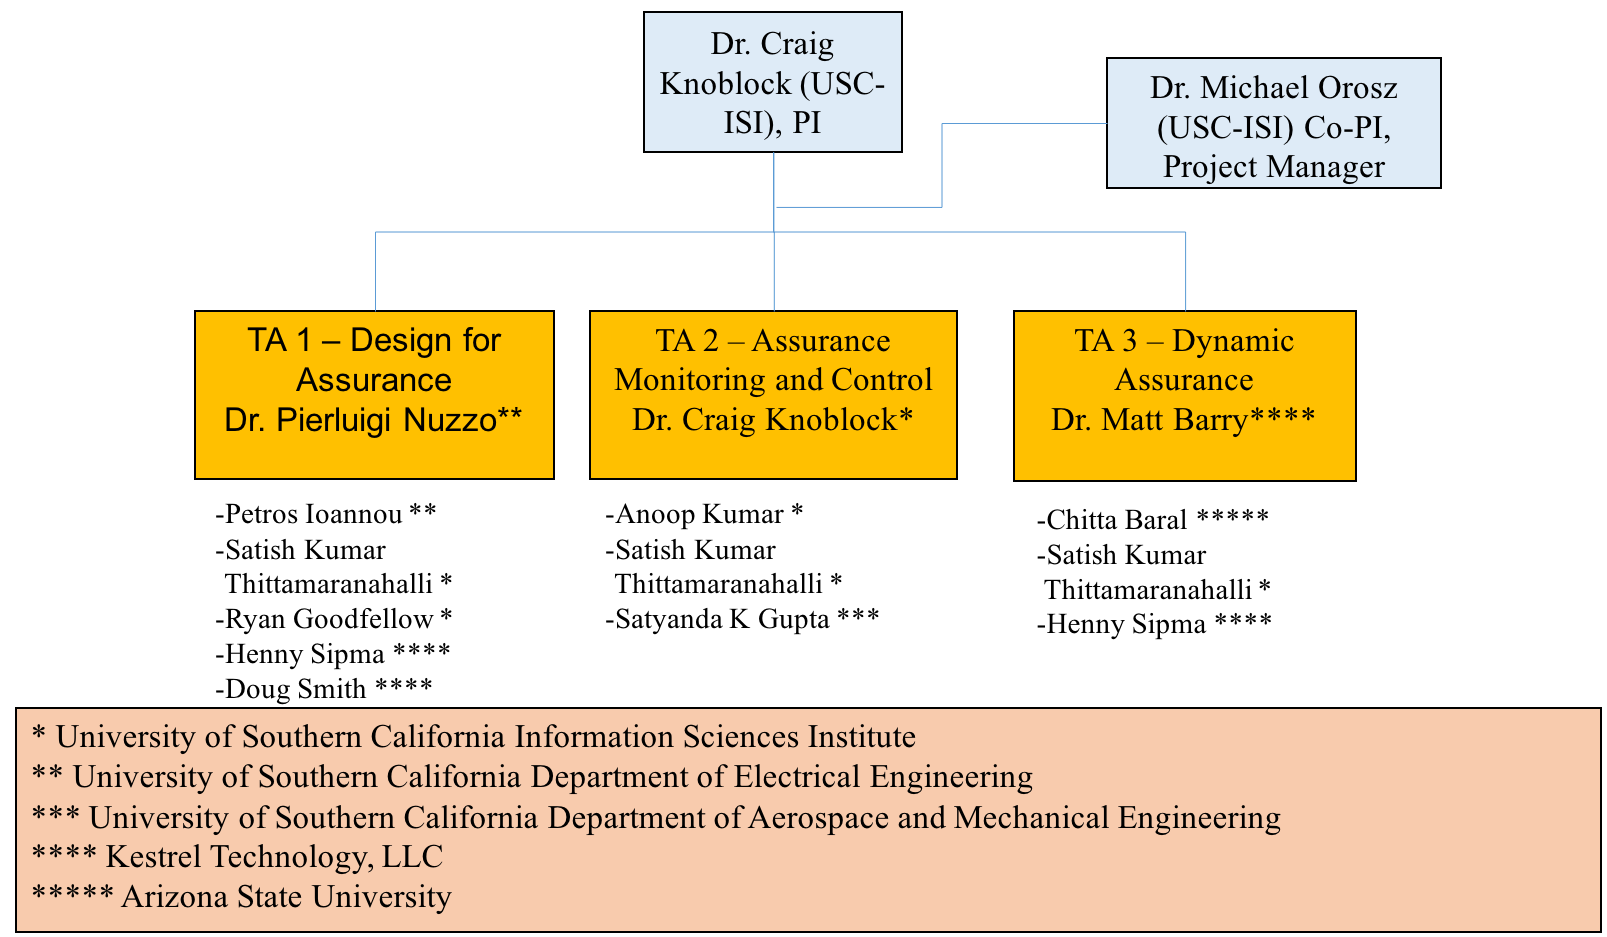
\includegraphics[width=6.0in]{./org-chart2.png}
\caption{\small Organization Chart}
\label{fig:org_chart}
\end{figure}

Coordination: To maximize collaboration and reduce risk to project failure from lack of communication and technical exchange, we plan to employ a wide variety of working styles and communication/coordination so that all can contribute.  At the core of our project will be regularly scheduled meetings bridging the diversely distributed team (Table~\ref{fig:Collaboration_Table}).  These meetings will address project status, identify challenges, implement risk mitigation strategies and participate in technology exchanges and system integration efforts (when appropriate)

\begin{table}[ht]
\caption{\small Project Meetings and Events}
  \centering
  {\footnotesize
\begin{tabular}{|m{3.15in}|m{3in}|} 
\hline
\textbf{Meeting} & \textbf{Frequency} 
\\\hline
Conference calls among investigators (discuss project status, address concerns and project risks) & Weekly
\\
\hline
Technical exchange and coordination meetings using Bluejeans or another videoconference technology & At least twice a month and more frequently as needed
  \\ 
\hline
Face-to-Face meetings (prior to P/I and demonstration meetings) & Every 3 to 6 months and more frequently (especially at the beginning of the project) as needed
 \\\cline{1-2}

\hline
\end{tabular}
}
\label{fig:Collaboration_Table}
\end{table}

\begin{table}[tbhp]
\caption{\small Key Project Team Member Responsibilities}
  \centering
  {\footnotesize
\begin{tabular}{| m{.75in} | m{3.9in}| m{1.5in}|} 
\hline
\textbf{Key Member} & \textbf{Responsibilities} & \textbf{Tasks} 
\\\hline
Dr.\ Craig Knoblock  & Principal Investigator responsible for project, leads TA 2 – Assurance Monitoring and Control.  Will lead the overall project and lead the TA2 team.  Served as the PI on many DARPA projects and has sucessfully led many large teams.    Effort on project:  25\% &
1.1.6, 1.2.2 1.2.3, 1.2.4, 1.3.4, 1.4.1, 
2.1.6, 2.2.2 2.2.3, 2.2.4, 2.3.4, 2.4.1, 
3.1.6, 3.2.2, 3.2.3, 3.2.4, 3.3.4, 3.4.1
\\
\hline
Dr.\ Michael Orosz & Co-Principal Investigator responsible managing the day-to-day operations of the project, assist technical teams as needed, coordinate with TA4 teams.    Has led many large complex multi-disciplined/multi-organizational projects in academic and industry environments.  Effort on project: 50\%
& 1.1.6, 2.1.6, 3.1.6, 1.4.1, 2.4.1, 3.4.1
  \\ 
\hline
Dr.\ Pierluigi Nuzzo 
& 
Co-Principal Investigator.  Leads the TA 1 - Design for Assurance team and conducts research on the formal methods for the design of the TA1 system.  Research experience on methodologies and tools for the design of cyber-physical systems; contracts, interfaces, and compositional methods for embedded system design; the application of automated formal methods and optimization theory to problems in embedded and cyber-physical systems.  Effort on project: 2 months/year (16.6\%)
& 
1.1.1, 2.1.1, 3.1.1 \\
\hline
Dr.\ Matthew Barry
& 
Key personnel.  Leads the TA 3 – Dynamic Assurance.   He will conduct the research on the dynamic assurance case language editors and parsers, the run-time system, and system integrations. Effort on project:  66\%
& 
1.3.2, 2.3.2, 3.3.2\\
\hline
Dr.\ Chitta Baral
& 
Key personnel responsible for learning assurance rules, supporting assurance rules with uncertainty and improving solver speed.  Expertise on ASP solvers, which will be used to reason about the assurance cases. Effort on project: 20\%
& 
1.3.1, 2.3.1, 3.3.1 \\
\hline
Dr.\ Doug Smith 
& 
Key personnel will support formal methods aspects of TA1, and lead the effort on abstract refinement. Expertise in field of automated correct-by-construction program generation.    Effort on project: 40\%
& 
1.1.5, 2.1.5, 3.1.5 \\
\hline
Dr.\ Henny Sipma
& 
Key personnel who will support the program verification tasks under TA1.  Will lead the effort on program verification.   Effort on project:  45\%
& 
1.1.5, 2.1.5, 3.1.5, 1.3.2, 2.3.2, 3.3.2 \\
\hline
Dr.\ Petros Ioannou
& 
Key personnel responsible providing and extending the assurance test bed, which will be available at the start of the project for autonomous vehicles.   Effort on project: 1 month/year (8.3\%)
& 
1.1.2, 2.1.2 (optional), 3.1.2 (optional)
\\
\hline
Dr.\ Satyandra Kumar Gupta
& 
Key Personnel providing autonomous command and control expertise to the TA-2 team.   Will lead the research on safety aware learning on TA2.   Past research on physics-aware decision making to facilitate automation.  Effort on project: 1 month/year (8.3\%)
& 
1.2.1, 2.2.1, 3.2.1 \\
\hline
Dr.\ Anoop Kumar 
& 
Key personnel providing support to the TA 2 project team.  Will lead the research on monitoring \& control and detecting distribution shifts.  Effort on project: 50\%
& 
1.2.1, 1.2.2, 1.2.3, 1.2.4, 2.2.1, 2.2.2, 2.2.3, 2.2.4, 3.2.1, 3.2.2, 3.2.3, 3.2.4\\
\hline
Dr.\ Satish Thittamaranahalli
& 
Key personnel developing scalable algorithms for TA1, TA2, and TA3 project teams.  Has extensive experience on scalable algorithm design, machine learning, and constraint reasoning.  Effort on project: 50\%
& 
1.2.1, 1.2.2, 1.2.3, 1.2.4, 2.2.1, 2.2.2, 2.2.3, 2.2.4, 3.2.1, 3.2.2, 3.2.3, 3.2.4, 1.1.4, 2.1.4, 3.1.4 \\
\hline
Dr.\ Ryan Goodfellow
& 
Key personnel providing support to the TA-1 project. Will lead the research on simulation-based testing.  Has extensive experience on simulation-based testing.  Effort on project:  30\%
& 
1.1.3, 2.1.3, 3.1.3 \\

\cline{1-2}

\hline
\end{tabular}
}
\label{fig:Table_Mgmt}
\end{table}



\newpage
\section{Personnel, Qualifications and Commitment}

{\bf Dr.\ Craig Knoblock}, the PI on this effort, is a Research Professor of both Computer Science and Spatial Sciences at the University of Southern California (USC) and Director of the Intelligent Systems Division at the USC Information Sciences Institute.   He received his Ph.D. from Carnegie Mellon University in computer science. 
%His research focuses on techniques for describing, acquiring, and exploiting the semantics of data.  
In previous projects he has worked on developing  scalable approaches to execution monitoring, accurate detection of sensor failures, and   automatic modeling and reconstruction of sensors.  He has published more than 300 journal articles, book chapters, and conference papers on these topics.  Dr. Knoblock is a Fellow of the Association for the Advancement of Artificial Intelligence (AAAI), a Distinguished Scientist of the Association of Computing Machinery (ACM), a Senior Member of IEEE, past President and Trustee of the International Joint Conference on Artificial Intelligence.
%and winner of the 2014 Robert S. Engelmore Award.  

{\bf Dr.\ Michael Orosz}, a Co-PI on this effort, is a Research Associate Professor of Civil and Environmental Engineering at the University of Southern California (USC) and Research Director of the Decision Systems Group at the USC Information Sciences Institute.  Dr. Orosz has over 30 years’ experience in commercial and government software development, basic and applied research, project management, academic research and has developed and deployed several commercially successful products.  His research interests are in machine learning and decision analytics as applied to intelligence analysis and autonomous command and control such as smart building controls.    Dr. Orosz has extensive experience in managing large complex multi-disciplined/multi-teamed research projects. %funded by DARPA, DHS, DoD, DoE, Industry, NASA, NRO, NSA and ONR.   
He received his Ph.D. in computer science from the University of California, Los Angeles.

{\bf Dr.\ Pierluigi Nuzzo}, a Co-PI on this project, is an Assistant Professor in the Department of Electrical Engineering at the University of Southern California. He received the Ph.D. in Electrical Engineering and Computer Sciences from the University of California at Berkeley. 
%in 2015, and the Laurea degree (MS) in electrical engineering (summa cum laude) from the University of Pisa, Italy, and the Sant'Anna School of Advanced Studies, Pisa, Italy.
%
%He has four years of research experience in analog and mixed signal circuit design as a researcher at IMEC, Leuven, Belgium, and over 10 years experience in design methodologies and tools for mixed-signal integrated circuits and cyber-physical systems, as a researcher at the University of Pisa, IMEC, UC Berkeley, and USC. 
His research interests
include: methodologies and tools for cyber-physical system and mixed-signal
system design; contracts, interfaces and compositional methods for embedded
system design; the application of formal methods and optimization theory to problems in embedded and cyber-physical systems and electronic design automation. 
%
Prof. Nuzzo received %First Place in the operational category and Best Overall
%Submission in the 2006 DAC/ISSCC Design Competition, 
a Marie Curie Fellowship
from the European Union in 2006, 
the University of California at Berkeley EECS
departmental fellowship in 2008, 
%the University of California at Berkeley Outstanding Graduate Student Instructor Award in 2013, 
the IBM Ph.D.
Fellowship in 2012 and 2014, 
%the Best Paper Award from the International Conference on Cyber-Physical Systems (ICCPS) in 2016, 
and the David J.~Sakrison Memorial Prize in 2016 for his doctoral research. 
%He is an author of 1 patent and over 60 publications.

{\bf Dr.\ Satyandra K. Gupta} is Smith International Professor in the Department of Aerospace and Mechanical Engineering at the University of Southern California. %Prior to joining the University of Southern California, he was a Professor in the Department of Mechanical Engineering and the Institute for Systems Research at the University of Maryland. He was the founding director of the Maryland Robotics Center and the Advanced Manufacturing Laboratory at the University of Maryland. 
He served as a program director for the National Robotics Initiative at the National Science Foundation from September 2012 to September 2014.  Dr. Gupta's interest is in the area of physics-aware decision making to facilitate automation. He has published more than 300 technical articles. He is a fellow of the American Society of Mechanical Engineers (ASME) and editor of ASME Journal of Computing and Information Science in Engineering. Dr. Gupta has received the Young Investigator Award from the Office of Naval Research in 2000, CAREER Award from the National Science Foundation in 2001, Presidential Early Career Award for Scientists and Engineers (PECASE) in 2001, Invention of the Year Award at the University of Maryland in 2007, Kos Ishii-Toshiba Award from ASME in 2011, and Excellence in Research Award from ASME in 2013.%, and Distinguished Alumnus Award from Indian Institute of Technology, Roorkee in 2014. %He has also received seven best paper awards at conferences.

{\bf Ryan Goodfellow} is a computer scientist at ISI working in combined cyber physical simulation and emulation platform development. His formal background is in simulation algorithms and modeling techniques using differential-algebraic equations (DAE). He has applied this knowledge in the CPS space by integrating DAE modeling languages and simulation engines with network testbeds to create comprehensive scientific experimentation platforms for cyber-physical systems. These experimentation platforms have been used in the power grid research space. %Ryan is a lead developer on the Deter network testbed, with a strong background in networked and distributed systems engineering. %He is also a combat veteran, serving as a non-commissioned officer and SIGINT team lead for a multi-functional intelligence team in Afghanistan.

{\bf Dr.\ Petros Ioannou} is a Professor in the Department of Electrical Engineering, Director of the Center for Advanced Transportation Technologies and Associate Director for Research for the DOT supported University Transportation Center at USC. He received his MS and PhD from the University of Illinois at Urbana Champaign in Mechanical and Electrical Engineering, respectively. His research interests are in robust adaptive control, vehicle dynamics and control, human factors and safety, automated vehicles, nonlinear systems and Intelligent transportation Systems.  He received the 2016 IEEE Transportation Technologies field award and the 2016 IEEE Control system society Transition to Practice Award. He is a Fellow of IEEE, IFAC and IET and author/coauthor of 8 books and over 400 papers.

{\bf Dr.\ Matthew Barry} will serve as lead for the TA3 tasks. %He will implement the dynamic assurance case language editors and parsers, the run-time system, and system integrations.  He will implement the assurance case arguments and the API for updating argument structure and content.  
Dr. Barry currently is CEO at Kestrel Technology LLC, and previously spent 20 years in NASA space mission operations at the Jet Propulsion Lab and Johnson Space Center.  At NASA Headquarters he led the introduction of dependability case requirements and plans for flight computing systems in upcoming manned space exploration missions, as well as the development of Agency-level software-related safety-critical control system requirements.  He recently served as a Principal Investigator on DHS/Cyber S\&T STAMP (Static Tool Analysis Modernization Program), DARPA CSFV (Crowd Sourced Formal Verification), three NASA Aeronautics R\&D projects, and the AFRL-sponsored Static Analysis of Numerical Algorithms project.  Dr. Barry earned BSME, MS, and PhD degrees in mechanical engineering, and an MBA degree, from Rice University.  

{\bf Dr.\ Henny Sipma} will support the program verification tasks under TA1.  %She is the key person behind the company's {\em KT Advance\/} and {\em KT Transferal\/} static analysis products, and the designer and programmer of the company's core {\em CodeHawk\/} abstract interpretation engine. 
Dr. Sipma currently is the CTO at Kestrel Technology LLC.  She has spent the past 10 years with Kestrel Technology as a static analysis expert; previously developed and taught static analysis techniques as senior research associate at Stanford University for eight years; and developed industrial process controls as an senior systems analyst at Shell.  She has been Principal Investigator or company lead on several recent R\&D projects for Federal agencies, including two projects under the IARPA STONESOUP (Securely Taking On New Executable Software of Uncertain Provenance) program; the DHS Cyber S\&T Gold Standard project; and the DARPA-sponsored STAC (Space-Time Analysis for Cybersecurity) and MUSE (Mining and Understanding Software Enclaves) programs.  Dr. Sipma earned 
%a BS degree in chemistry and an MS degree in chemical engineering at the University of Groningen in The Netherlands, and 
MS and PhD degrees in computer science from Stanford University.  

{\bf Dr.\ Douglas R.\ Smith} will support formal methods aspects of TA1, including the enforcement of safety properties and the generation of monitors.  He is President of Kestrel Technology LLC and Principal Scientist at Kestrel Institute.  He is a Fellow of the American Association of Artificial Intelligence (AAAI) and an ASE Fellow (Automated Software Engineering).  From 1986 to 2000, he taught an advanced graduate course on correct-by-construction software development at Stanford.  
%Dr. Smith has led the development of a series of software synthesis systems, including KIDS (Kestrel Interactive Development System), Specware, Designware, and Planware. 
%Applications domains have included a variety of complex high-performance planners and schedulers for the US Air Force.  He leads current projects on the generation of air mission plans and cyberoperations.  
Other recent projects focused on automated policy enforcement \cite{SmithD0703,SmithD08}, synthesis of secure network protocol codes, and the synthesis of high-performance constraint-solvers\cite{SmithD08c,SmithD13}.  Dr. Smith has over 30 years experience in the field of automated correct-by-construction program generation and has published over 100 papers. He has one patent.  He received the Ph.D. in Computer Science from Duke University% in 1979.  

{\bf Dr. Chitta Baral} is a Professor in the Department of Computer Science and Engineering at Arizona State University. He will support the TA3 efforts on Learning assurance rules, supporting assurance rules with uncertainty and improving solver speed. Dr. Baral has expertise in various aspects of autonomy and Artificial Intelligence. 
He wrote the first book on answer set programming (published by Cambridge University Press) the formal language behind our assurance rules. Some of his other works relevant to this proposal are: goal specification for autonomous systems, automatic construction of control rules for autonomous systems that satisfy given goals, combining machine learning with reasoning in various contexts, including image understanding. %He is the President of KR Inc. He is an associate editor of AIJ and has been an associate editor of JAIR.

{\bf Dr.\ Satish Kumar Thittamaranahalli (T. K. Satish Kumar)} leads the Collaboratory for Algorithmic Techniques and Artificial Intelligence (CATAI) at USC's Information Sciences Institute. He has published over 60 papers on numerous topics in Artificial Intelligence spanning such diverse areas as Constraint Reasoning, Planning and Scheduling, Probabilistic Reasoning, Robotics, Combinatorial Optimization, Approximation and Randomization, Heuristic Search, Model-Based Reasoning, Knowledge Representation and Spatio-Temporal Reasoning. %He %has served on the Program Committees of many international conferences in Artificial Intelligence
He and is a winner of the 2016 Best Robotics Paper Award and the 2005 Best Student Paper Award from the International Conference on Automated Planning and Scheduling. 
Dr. Kumar received his PhD in Computer Science from Stanford University. %In the past, he has also been a Visiting Student at the NASA Ames Research Center, a Postdoctoral Research Scholar at the University of California, Berkeley, a Research Scientist at the Institute for Human and Machine Cognition, a Visiting Assistant Professor at the University of West Florida, and a Senior Research and Development Scientist at Mission Critical Technologies.

\textbf{Dr.\ Anoop Kumar} is a senior computer scientist at USC ISI and has broad expertise in machine learning, statistical modeling, and software engineering.  Dr.\ Kumar is the technical lead on the DARPA RSPACE program and has played a vital role in developing a system that fuses air operations data from multiple sources, maintains world state, and issues warnings. Previously, he led the research and development of the BBN’s election forecasting system for the IARPA OSI program. %Dr.\ Kumar played a significant role in the DARPA DEFT program by developing a model to support integration of output from multiple NLP algorithms. He has contributed at the development to management levels on government research contracts and commercial projects. 
Dr.\ Kumar helped design and develop BBN's commercially available, hosted speech and medical transcription services offering. 

\begin{table}[!tbh]
\begin{footnotesize}
\vspace{-0.1in}

\begin{tabular}{lll}
\begin{tabular}[t]{|l|@{}c@{}|@{}c@{}|@{}c@{}|@{}c@{}|} \hline
Project & Status & \multicolumn{3}{ c| }{Hours} \\ \cline{3-5}
& & P1 & P2 & P3 \\ \hline



\multicolumn{5}{ |c| }{ \textbf{Craig Knoblock} } \\ \cline{1-5}
Safeguard & Pro & 770 & 641 & 641 \\ \cline{1-5}
ELICIT & Cur & 308 & 256 & 120 \\ \cline{1-5}
WTNIC & Cur & 11 & 0 & 0 \\ \cline{1-5}
EFFECT & Cur & 641 & 107 & 0 \\ \cline{1-5}
LinkedMaps & Cur & 203 & 25 & 0 \\ \cline{1-5}
PRINCESS & Cur & 608 & 96 & 0 \\ \cline{1-5}
SCHARP & Cur & 481 & 54 & 0 \\ \cline{1-5}
MINT & Pen & 650 & 534 & 285 \\ \cline{1-5}

\multicolumn{5}{ |c| }{ \textbf{Michael Orosz} } \\ \cline{1-5}
Safeguard & Pro & 1560 & 1300 & 1300  \\ \cline{1-5}
SMC/SY & Cur & 1803 & 0 & 0  \\ \cline{1-5}

\multicolumn{5}{ |c| }{ \textbf{Matthew Barry} } \\ \cline{1-5}
Safeguard & Pro & 2078 & 1690 & 1554 \\ \cline{1-5}
Starlite & Cur & 1840 & 1692 & 0 \\ \cline{1-5}



\multicolumn{5}{ |c| }{ \textbf{Anoop Kumar} } \\ \cline{1-5}
Safeguard & Pro & 1560 & 1300 & 1300 \\ \cline{1-5}

\end{tabular}
&
\begin{tabular}[t]{|l|@{}c@{}|@{}c@{}|@{}c@{}|@{}c@{}|} \hline
Project & Status & \multicolumn{3}{ c| }{Hours} \\ \cline{3-5}
& & P1 & P2 & P3 \\ \hline

\multicolumn{5}{ |c| }{ \textbf{Pierluigi Nuzzo} } \\ \cline{1-5}
Safeguard & Pro & 520 & 433 & 433  \\ \cline{1-5}
Mirage & Cur & 433 & 0 & 0  \\ \cline{1-5}

\multicolumn{5}{ |c| }{ \textbf{Satyandra Gupta} } \\ \cline{1-5}
Safeguard & Pro & 260 & 217 & 217 \\ \cline{1-5}
Human   & Cur & 22 & 0 & 0 \\ \cline{1-5}
Vehicles & Cur & 36 & 0 & 0 \\ \cline{1-5}
Robot & Cur & 116 & 0 & 0 \\ \cline{1-5}
Assembly & Cur & 33 & 0 & 0 \\ \cline{1-5}
Solar & Cur & 4 & 0 & 0 \\ \cline{1-5}

\multicolumn{5}{ |c| }{ \textbf{Petros Ioannou} } \\ \cline{1-5}
Safeguard & Pro & 260 & 217 & 217 \\ \cline{1-5}
CPS & Cur & 130 & 0 & 0 \\ \cline{1-5}

\multicolumn{5}{ |c| }{ \textbf{Ryan Goodfellow} } \\ \cline{1-5}
Safeguard & Pro & 936 & 780 & 780 \\ \cline{1-5}
STEAM & Cur & 416 & 0 & 0 \\ \cline{1-5}


\end{tabular}
&
\begin{tabular}[t]{|l|@{}c@{}|@{}c@{}|@{}c@{}|@{}c@{}|} \hline
Project & Status & \multicolumn{3}{ c| }{Hours} \\ \cline{3-5}
& & P1 & P2 & P3 \\ \hline

\multicolumn{5}{ |c| }{ \textbf{Chitta Baral} } \\ \cline{1-5}
Safeguard & Pro & 659 & 485 & 485 \\ \cline{1-5}
PostdocBP & Cur & 176 & 0 & 0 \\ \cline{1-5}
Languages & Pen & 528 & 264 & 264 \\ \cline{1-5}
CAREER & Pen & 88 & 44 & 44 \\ \cline{1-5}
CHS & Pen & 510 & 255 & 0 \\ \cline{1-5}

\multicolumn{5}{ |c| }{ \textbf{Doug Smith} } \\ \cline{1-5}
Safeguard & Pro & 1222 & 984 & 840 \\ \cline{1-5}
RSPACE & Cur & 342 & 0 & 0 \\ 
\cline{1-5}
PLANX & Cur & 154 & 0 & 0 \\ 
\cline{1-5}
HACCS & Pen & 923 & 769 & 769 \\ 
\cline{1-5}

\multicolumn{5}{ |c| }{ \textbf{Henny Sipma} } \\ \cline{1-5}
Safeguard & Pro & 1372 & 962 & 840 \\ \cline{1-5}
STAC & Cur & 797 & 0 & 0 \\ \cline{1-5}

\multicolumn{5}{ |c| }{ \textbf{Satish Thittamaranahalli} } \\ \cline{1-5}
Safeguard & Pro & 1560 & 1300 & 1300 \\ \cline{1-5}
MapF & Cur & 103 & 103 & 0 \\ \cline{1-5}

\end{tabular}
\end{tabular}

\end{footnotesize}
\caption{Individual commitments of key personnel}
\label{tab:Commitments}
\vspace{-0.2in}
\end{table}

\clearpage
\newpage
\section{Capabilities}


%\subsection{University of Southern California}
USC has strengths in number of areas that are closely related to the proposed work:
\begin{itemize}[itemsep=0pt,leftmargin=*]
\item Dr.\ Nuzzo 
%has over 10-year research experience in embedded system design, from mixed-signal chip design (analog-to-digital converters, frequency synthesizers, software-defined radio), to methodologies and tools for mixed-signal integrated circuits and Cyber-Physical Systems (CPSs), and the application of formal methods and optimization theory to problems in embedded and cyber-physical systems and electronic design automation.  
%His doctoral work 
has done extensive research on contracts and compositional methods for heterogeneous system design and design space exploration, with application to aircraft electric power systems and environmental control systems. His work has helped transition rigorous system design foundations, innovative design methodologies, and new systems engineering paradigms to industry (IBM, United Technologies). 
\item Dr.\ Satyandra K. Gupta has worked on autonomous surface vehicles, autonomous ground vehicles for operation on rugged terrains, and autonomous flapping wing aerial vehicles.   His group has developed a hierarchal decision making approach for realizing autonomous systems. 
%This approach combines task planning and assignment, deliberative trajectory planning, reactive collision avoidance behaviors, and trajectory tracking control layers. 
His group has also developed new methods for learning reactive behaviors in adversarial environments and COLREGS compliant trajectory planning. \item Dr.\ Knoblock has developed methods that learn the relationships between sensors to both identify failures and changes in sensor and reconstruct those sensors, providing estimates of the accuracy of the reconstructed sensors.  
\item Ryan Goodfellow has extensive experience in simulation based testing through high-fidelity CPS testbed environment development and operation, using the Deter network testbed as the core which has supported several large scale government projects from a variety of agencies and thousands of users. %we have developed sophisticated CPS experiments under programs such as NFS RIPS, NIST SmartCities and the DHS Cybersecurity showcase.
\item Dr.\ Ioannou %helped  design and implement adaptive cruise control systems in collaboration with Ford Motor Company, which was commercialized four years before any other company. He 
worked on several DOT funded projects on automated vehicles and intelligent highway systems where he demonstrated his vehicle control designs for safety and performance on actual automated vehicles in test trucks and I-15 highway.
\item Drs.\ Knoblock, Kumar, and Thittamaranahalli have developed highly scalable approaches for monitoring message traffic to identify potential problems and issue warnings and alerts. 
\item Dr. Thittamaranahalli has developed state-of-the-art methods for efficiently solving large-scale search and optimization problems. %These techniques will be applicable in TA2 for safety-aware learning and planning, in TA2 for assurance monitoring and control, and in TA3 for dynamic assessment of assurance cases.

\end{itemize}
%\subsection{Kestrel Technology LLC}

Kestrel Technology's strength is in program analysis, specifically static analysis of both source and binary targets.  The company performs applied R\&D and product development for a variety of static analysis applications  pivoting primarily on the abstract interpretation technique.  The company recently initiated development of program analysis applications using logical equivalence techniques. As a provider of verification evidence in the form of mathematical proofs, the company also has expertise in the design and development of assurance case arguments for high-integrity systems using such evidence. %The company is engaged in a partnership with Wind River Systems to develop program analysis tools for its embedded system developers.  Many of Wind River's customers must develop their products under safety and certification standards, including those using safety cases.  

   

%\subsection{Arizona State University}
Chitta Baral at Arizona State University has developed various software to learn assurance rules and various ASP solvers, which he has made available as open-source.

Most of the software carried forward for implementation or derivation is open source.  The single exception is Kestrel Technology's {\it KT Advance\/} static analysis tool (TA1), in particular the abstract interpretation engine therein, which is company proprietary and is US EAR export-controlled.   
%Owing to mixed funding for the development of that technology 
We will continue to provide the Federal government a restricted use license for that particular item.

There are no specialized facilities, data, or GFE required for this effort. 

\include{sow}
\include{milestones}

% \section{Level of Effort by Task \textcolor{red}{[Mike/Lisa - 1 pages]}}

% \textcolor{blue}{
% \begin{itemize}
% \item Will be a separate spreadsheet
% \item
% \end{itemize}
% }

\include{appendix_a}

%\section{Appendix B \textcolor{red}{[No Page Count]}}

\section{References}
\bibliographystyle{acm} 
\bibliography{TA3/ta3,TA2/ta2,TA1/ta1}
\end{document}
\clearpage
\newpage


\section{Management Plan}


The Principal Investigator for this effort is Dr. Craig Knoblock who is responsible for all aspects of the effort, will coordinate the parallel team efforts, and will ensure high levels of performance from individual team members.  The Co-P/I, Dr. Michael Orosz, will provide project management and will assist all performers in the execution of the project.    The project team is divided into three working groups (Figure~\ref{fig:org_chart}) corresponding to Technical Areas 1-3, however, members of each team contribute across all project activities.   Table~\ref{fig:Table_Mgmt} defines the major contributions of each project team member to the project tasks.

\begin{figure}[tbhp]
%\vspace{-25pt}
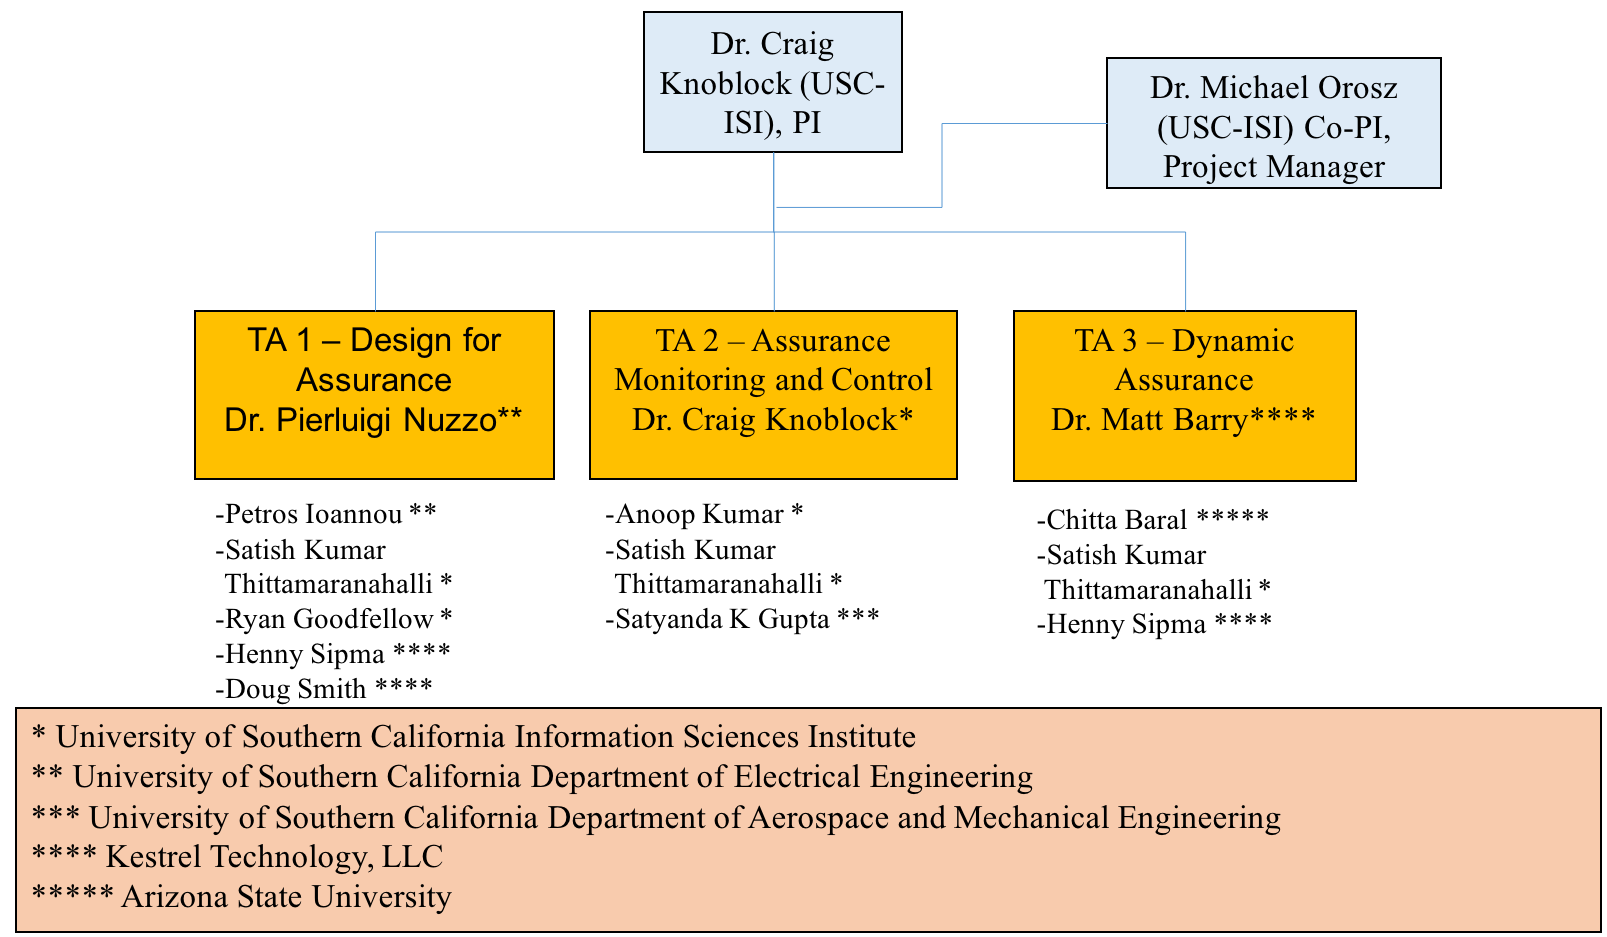
\includegraphics[width=6.0in]{./org-chart2.png}
\caption{\small Organization Chart}
\label{fig:org_chart}
\end{figure}

Coordination: To maximize collaboration and reduce risk to project failure from lack of communication and technical exchange, we plan to employ a wide variety of working styles and communication/coordination so that all can contribute.  At the core of our project will be regularly scheduled meetings bridging the diversely distributed team (Table~\ref{fig:Collaboration_Table}).  These meetings will address project status, identify challenges, implement risk mitigation strategies and participate in technology exchanges and system integration efforts (when appropriate)

\begin{table}[ht]
\caption{\small Project Meetings and Events}
  \centering
  {\footnotesize
\begin{tabular}{|m{3.15in}|m{3in}|} 
\hline
\textbf{Meeting} & \textbf{Frequency} 
\\\hline
Conference calls among investigators (discuss project status, address concerns and project risks) & Weekly
\\
\hline
Technical exchange and coordination meetings using Bluejeans or another videoconference technology & At least twice a month and more frequently as needed
  \\ 
\hline
Face-to-Face meetings (prior to P/I and demonstration meetings) & Every 3 to 6 months and more frequently (especially at the beginning of the project) as needed
 \\\cline{1-2}

\hline
\end{tabular}
}
\label{fig:Collaboration_Table}
\end{table}

\begin{table}[tbhp]
\caption{\small Key Project Team Member Responsibilities}
  \centering
  {\footnotesize
\begin{tabular}{| m{.75in} | m{3.9in}| m{1.5in}|} 
\hline
\textbf{Key Member} & \textbf{Responsibilities} & \textbf{Tasks} 
\\\hline
Dr.\ Craig Knoblock  & Principal Investigator responsible for project, leads TA 2 – Assurance Monitoring and Control.  Will lead the overall project and lead the TA2 team.  Served as the PI on many DARPA projects and has sucessfully led many large teams.    Effort on project:  25\% &
1.1.6, 1.2.2 1.2.3, 1.2.4, 1.3.4, 1.4.1, 
2.1.6, 2.2.2 2.2.3, 2.2.4, 2.3.4, 2.4.1, 
3.1.6, 3.2.2, 3.2.3, 3.2.4, 3.3.4, 3.4.1
\\
\hline
Dr.\ Michael Orosz & Co-Principal Investigator responsible managing the day-to-day operations of the project, assist technical teams as needed, coordinate with TA4 teams.    Has led many large complex multi-disciplined/multi-organizational projects in academic and industry environments.  Effort on project: 50\%
& 1.1.6, 2.1.6, 3.1.6, 1.4.1, 2.4.1, 3.4.1
  \\ 
\hline
Dr.\ Pierluigi Nuzzo 
& 
Co-Principal Investigator.  Leads the TA 1 - Design for Assurance team and conducts research on the formal methods for the design of the TA1 system.  Research experience on methodologies and tools for the design of cyber-physical systems; contracts, interfaces, and compositional methods for embedded system design; the application of automated formal methods and optimization theory to problems in embedded and cyber-physical systems.  Effort on project: 2 months/year (16.6\%)
& 
1.1.1, 2.1.1, 3.1.1 \\
\hline
Dr.\ Matthew Barry
& 
Key personnel.  Leads the TA 3 – Dynamic Assurance.   He will conduct the research on the dynamic assurance case language editors and parsers, the run-time system, and system integrations. Effort on project:  66\%
& 
1.3.2, 2.3.2, 3.3.2\\
\hline
Dr.\ Chitta Baral
& 
Key personnel responsible for learning assurance rules, supporting assurance rules with uncertainty and improving solver speed.  Expertise on ASP solvers, which will be used to reason about the assurance cases. Effort on project: 20\%
& 
1.3.1, 2.3.1, 3.3.1 \\
\hline
Dr.\ Doug Smith 
& 
Key personnel will support formal methods aspects of TA1, and lead the effort on abstract refinement. Expertise in field of automated correct-by-construction program generation.    Effort on project: 40\%
& 
1.1.5, 2.1.5, 3.1.5 \\
\hline
Dr.\ Henny Sipma
& 
Key personnel who will support the program verification tasks under TA1.  Will lead the effort on program verification.   Effort on project:  45\%
& 
1.1.5, 2.1.5, 3.1.5, 1.3.2, 2.3.2, 3.3.2 \\
\hline
Dr.\ Petros Ioannou
& 
Key personnel responsible providing and extending the assurance test bed, which will be available at the start of the project for autonomous vehicles.   Effort on project: 1 month/year (8.3\%)
& 
1.1.2, 2.1.2 (optional), 3.1.2 (optional)
\\
\hline
Dr.\ Satyandra Kumar Gupta
& 
Key Personnel providing autonomous command and control expertise to the TA-2 team.   Will lead the research on safety aware learning on TA2.   Past research on physics-aware decision making to facilitate automation.  Effort on project: 1 month/year (8.3\%)
& 
1.2.1, 2.2.1, 3.2.1 \\
\hline
Dr.\ Anoop Kumar 
& 
Key personnel providing support to the TA 2 project team.  Will lead the research on monitoring \& control and detecting distribution shifts.  Effort on project: 50\%
& 
1.2.1, 1.2.2, 1.2.3, 1.2.4, 2.2.1, 2.2.2, 2.2.3, 2.2.4, 3.2.1, 3.2.2, 3.2.3, 3.2.4\\
\hline
Dr.\ Satish Thittamaranahalli
& 
Key personnel developing scalable algorithms for TA1, TA2, and TA3 project teams.  Has extensive experience on scalable algorithm design, machine learning, and constraint reasoning.  Effort on project: 50\%
& 
1.2.1, 1.2.2, 1.2.3, 1.2.4, 2.2.1, 2.2.2, 2.2.3, 2.2.4, 3.2.1, 3.2.2, 3.2.3, 3.2.4, 1.1.4, 2.1.4, 3.1.4 \\
\hline
Dr.\ Ryan Goodfellow
& 
Key personnel providing support to the TA-1 project. Will lead the research on simulation-based testing.  Has extensive experience on simulation-based testing.  Effort on project:  30\%
& 
1.1.3, 2.1.3, 3.1.3 \\

\cline{1-2}

\hline
\end{tabular}
}
\label{fig:Table_Mgmt}
\end{table}



\newpage
\section{Personnel, Qualifications and Commitment}

{\bf Dr.\ Craig Knoblock}, the PI on this effort, is a Research Professor of both Computer Science and Spatial Sciences at the University of Southern California (USC) and Director of the Intelligent Systems Division at the USC Information Sciences Institute.   He received his Ph.D. from Carnegie Mellon University in computer science. 
%His research focuses on techniques for describing, acquiring, and exploiting the semantics of data.  
In previous projects he has worked on developing  scalable approaches to execution monitoring, accurate detection of sensor failures, and   automatic modeling and reconstruction of sensors.  He has published more than 300 journal articles, book chapters, and conference papers on these topics.  Dr. Knoblock is a Fellow of the Association for the Advancement of Artificial Intelligence (AAAI), a Distinguished Scientist of the Association of Computing Machinery (ACM), a Senior Member of IEEE, past President and Trustee of the International Joint Conference on Artificial Intelligence.
%and winner of the 2014 Robert S. Engelmore Award.  

{\bf Dr.\ Michael Orosz}, a Co-PI on this effort, is a Research Associate Professor of Civil and Environmental Engineering at the University of Southern California (USC) and Research Director of the Decision Systems Group at the USC Information Sciences Institute.  Dr. Orosz has over 30 years’ experience in commercial and government software development, basic and applied research, project management, academic research and has developed and deployed several commercially successful products.  His research interests are in machine learning and decision analytics as applied to intelligence analysis and autonomous command and control such as smart building controls.    Dr. Orosz has extensive experience in managing large complex multi-disciplined/multi-teamed research projects. %funded by DARPA, DHS, DoD, DoE, Industry, NASA, NRO, NSA and ONR.   
He received his Ph.D. in computer science from the University of California, Los Angeles.

{\bf Dr.\ Pierluigi Nuzzo}, a Co-PI on this project, is an Assistant Professor in the Department of Electrical Engineering at the University of Southern California. He received the Ph.D. in Electrical Engineering and Computer Sciences from the University of California at Berkeley. 
%in 2015, and the Laurea degree (MS) in electrical engineering (summa cum laude) from the University of Pisa, Italy, and the Sant'Anna School of Advanced Studies, Pisa, Italy.
%
%He has four years of research experience in analog and mixed signal circuit design as a researcher at IMEC, Leuven, Belgium, and over 10 years experience in design methodologies and tools for mixed-signal integrated circuits and cyber-physical systems, as a researcher at the University of Pisa, IMEC, UC Berkeley, and USC. 
His research interests
include: methodologies and tools for cyber-physical system and mixed-signal
system design; contracts, interfaces and compositional methods for embedded
system design; the application of formal methods and optimization theory to problems in embedded and cyber-physical systems and electronic design automation. 
%
Prof. Nuzzo received %First Place in the operational category and Best Overall
%Submission in the 2006 DAC/ISSCC Design Competition, 
a Marie Curie Fellowship
from the European Union in 2006, 
the University of California at Berkeley EECS
departmental fellowship in 2008, 
%the University of California at Berkeley Outstanding Graduate Student Instructor Award in 2013, 
the IBM Ph.D.
Fellowship in 2012 and 2014, 
%the Best Paper Award from the International Conference on Cyber-Physical Systems (ICCPS) in 2016, 
and the David J.~Sakrison Memorial Prize in 2016 for his doctoral research. 
%He is an author of 1 patent and over 60 publications.

{\bf Dr.\ Satyandra K. Gupta} is Smith International Professor in the Department of Aerospace and Mechanical Engineering at the University of Southern California. %Prior to joining the University of Southern California, he was a Professor in the Department of Mechanical Engineering and the Institute for Systems Research at the University of Maryland. He was the founding director of the Maryland Robotics Center and the Advanced Manufacturing Laboratory at the University of Maryland. 
He served as a program director for the National Robotics Initiative at the National Science Foundation from September 2012 to September 2014.  Dr. Gupta's interest is in the area of physics-aware decision making to facilitate automation. He has published more than 300 technical articles. He is a fellow of the American Society of Mechanical Engineers (ASME) and editor of ASME Journal of Computing and Information Science in Engineering. Dr. Gupta has received the Young Investigator Award from the Office of Naval Research in 2000, CAREER Award from the National Science Foundation in 2001, Presidential Early Career Award for Scientists and Engineers (PECASE) in 2001, Invention of the Year Award at the University of Maryland in 2007, Kos Ishii-Toshiba Award from ASME in 2011, and Excellence in Research Award from ASME in 2013.%, and Distinguished Alumnus Award from Indian Institute of Technology, Roorkee in 2014. %He has also received seven best paper awards at conferences.

{\bf Ryan Goodfellow} is a computer scientist at ISI working in combined cyber physical simulation and emulation platform development. His formal background is in simulation algorithms and modeling techniques using differential-algebraic equations (DAE). He has applied this knowledge in the CPS space by integrating DAE modeling languages and simulation engines with network testbeds to create comprehensive scientific experimentation platforms for cyber-physical systems. These experimentation platforms have been used in the power grid research space. %Ryan is a lead developer on the Deter network testbed, with a strong background in networked and distributed systems engineering. %He is also a combat veteran, serving as a non-commissioned officer and SIGINT team lead for a multi-functional intelligence team in Afghanistan.

{\bf Dr.\ Petros Ioannou} is a Professor in the Department of Electrical Engineering, Director of the Center for Advanced Transportation Technologies and Associate Director for Research for the DOT supported University Transportation Center at USC. He received his MS and PhD from the University of Illinois at Urbana Champaign in Mechanical and Electrical Engineering, respectively. His research interests are in robust adaptive control, vehicle dynamics and control, human factors and safety, automated vehicles, nonlinear systems and Intelligent transportation Systems.  He received the 2016 IEEE Transportation Technologies field award and the 2016 IEEE Control system society Transition to Practice Award. He is a Fellow of IEEE, IFAC and IET and author/coauthor of 8 books and over 400 papers.

{\bf Dr.\ Matthew Barry} will serve as lead for the TA3 tasks. %He will implement the dynamic assurance case language editors and parsers, the run-time system, and system integrations.  He will implement the assurance case arguments and the API for updating argument structure and content.  
Dr. Barry currently is CEO at Kestrel Technology LLC, and previously spent 20 years in NASA space mission operations at the Jet Propulsion Lab and Johnson Space Center.  At NASA Headquarters he led the introduction of dependability case requirements and plans for flight computing systems in upcoming manned space exploration missions, as well as the development of Agency-level software-related safety-critical control system requirements.  He recently served as a Principal Investigator on DHS/Cyber S\&T STAMP (Static Tool Analysis Modernization Program), DARPA CSFV (Crowd Sourced Formal Verification), three NASA Aeronautics R\&D projects, and the AFRL-sponsored Static Analysis of Numerical Algorithms project.  Dr. Barry earned BSME, MS, and PhD degrees in mechanical engineering, and an MBA degree, from Rice University.  

{\bf Dr.\ Henny Sipma} will support the program verification tasks under TA1.  %She is the key person behind the company's {\em KT Advance\/} and {\em KT Transferal\/} static analysis products, and the designer and programmer of the company's core {\em CodeHawk\/} abstract interpretation engine. 
Dr. Sipma currently is the CTO at Kestrel Technology LLC.  She has spent the past 10 years with Kestrel Technology as a static analysis expert; previously developed and taught static analysis techniques as senior research associate at Stanford University for eight years; and developed industrial process controls as an senior systems analyst at Shell.  She has been Principal Investigator or company lead on several recent R\&D projects for Federal agencies, including two projects under the IARPA STONESOUP (Securely Taking On New Executable Software of Uncertain Provenance) program; the DHS Cyber S\&T Gold Standard project; and the DARPA-sponsored STAC (Space-Time Analysis for Cybersecurity) and MUSE (Mining and Understanding Software Enclaves) programs.  Dr. Sipma earned 
%a BS degree in chemistry and an MS degree in chemical engineering at the University of Groningen in The Netherlands, and 
MS and PhD degrees in computer science from Stanford University.  

{\bf Dr.\ Douglas R.\ Smith} will support formal methods aspects of TA1, including the enforcement of safety properties and the generation of monitors.  He is President of Kestrel Technology LLC and Principal Scientist at Kestrel Institute.  He is a Fellow of the American Association of Artificial Intelligence (AAAI) and an ASE Fellow (Automated Software Engineering).  From 1986 to 2000, he taught an advanced graduate course on correct-by-construction software development at Stanford.  
%Dr. Smith has led the development of a series of software synthesis systems, including KIDS (Kestrel Interactive Development System), Specware, Designware, and Planware. 
%Applications domains have included a variety of complex high-performance planners and schedulers for the US Air Force.  He leads current projects on the generation of air mission plans and cyberoperations.  
Other recent projects focused on automated policy enforcement \cite{SmithD0703,SmithD08}, synthesis of secure network protocol codes, and the synthesis of high-performance constraint-solvers\cite{SmithD08c,SmithD13}.  Dr. Smith has over 30 years experience in the field of automated correct-by-construction program generation and has published over 100 papers. He has one patent.  He received the Ph.D. in Computer Science from Duke University% in 1979.  

{\bf Dr. Chitta Baral} is a Professor in the Department of Computer Science and Engineering at Arizona State University. He will support the TA3 efforts on Learning assurance rules, supporting assurance rules with uncertainty and improving solver speed. Dr. Baral has expertise in various aspects of autonomy and Artificial Intelligence. 
He wrote the first book on answer set programming (published by Cambridge University Press) the formal language behind our assurance rules. Some of his other works relevant to this proposal are: goal specification for autonomous systems, automatic construction of control rules for autonomous systems that satisfy given goals, combining machine learning with reasoning in various contexts, including image understanding. %He is the President of KR Inc. He is an associate editor of AIJ and has been an associate editor of JAIR.

{\bf Dr.\ Satish Kumar Thittamaranahalli (T. K. Satish Kumar)} leads the Collaboratory for Algorithmic Techniques and Artificial Intelligence (CATAI) at USC's Information Sciences Institute. He has published over 60 papers on numerous topics in Artificial Intelligence spanning such diverse areas as Constraint Reasoning, Planning and Scheduling, Probabilistic Reasoning, Robotics, Combinatorial Optimization, Approximation and Randomization, Heuristic Search, Model-Based Reasoning, Knowledge Representation and Spatio-Temporal Reasoning. %He %has served on the Program Committees of many international conferences in Artificial Intelligence
He and is a winner of the 2016 Best Robotics Paper Award and the 2005 Best Student Paper Award from the International Conference on Automated Planning and Scheduling. 
Dr. Kumar received his PhD in Computer Science from Stanford University. %In the past, he has also been a Visiting Student at the NASA Ames Research Center, a Postdoctoral Research Scholar at the University of California, Berkeley, a Research Scientist at the Institute for Human and Machine Cognition, a Visiting Assistant Professor at the University of West Florida, and a Senior Research and Development Scientist at Mission Critical Technologies.

\textbf{Dr.\ Anoop Kumar} is a senior computer scientist at USC ISI and has broad expertise in machine learning, statistical modeling, and software engineering.  Dr.\ Kumar is the technical lead on the DARPA RSPACE program and has played a vital role in developing a system that fuses air operations data from multiple sources, maintains world state, and issues warnings. Previously, he led the research and development of the BBN’s election forecasting system for the IARPA OSI program. %Dr.\ Kumar played a significant role in the DARPA DEFT program by developing a model to support integration of output from multiple NLP algorithms. He has contributed at the development to management levels on government research contracts and commercial projects. 
Dr.\ Kumar helped design and develop BBN's commercially available, hosted speech and medical transcription services offering. 

\begin{table}[!tbh]
\begin{footnotesize}
\vspace{-0.1in}

\begin{tabular}{lll}
\begin{tabular}[t]{|l|@{}c@{}|@{}c@{}|@{}c@{}|@{}c@{}|} \hline
Project & Status & \multicolumn{3}{ c| }{Hours} \\ \cline{3-5}
& & P1 & P2 & P3 \\ \hline



\multicolumn{5}{ |c| }{ \textbf{Craig Knoblock} } \\ \cline{1-5}
Safeguard & Pro & 770 & 641 & 641 \\ \cline{1-5}
ELICIT & Cur & 308 & 256 & 120 \\ \cline{1-5}
WTNIC & Cur & 11 & 0 & 0 \\ \cline{1-5}
EFFECT & Cur & 641 & 107 & 0 \\ \cline{1-5}
LinkedMaps & Cur & 203 & 25 & 0 \\ \cline{1-5}
PRINCESS & Cur & 608 & 96 & 0 \\ \cline{1-5}
SCHARP & Cur & 481 & 54 & 0 \\ \cline{1-5}
MINT & Pen & 650 & 534 & 285 \\ \cline{1-5}

\multicolumn{5}{ |c| }{ \textbf{Michael Orosz} } \\ \cline{1-5}
Safeguard & Pro & 1560 & 1300 & 1300  \\ \cline{1-5}
SMC/SY & Cur & 1803 & 0 & 0  \\ \cline{1-5}

\multicolumn{5}{ |c| }{ \textbf{Matthew Barry} } \\ \cline{1-5}
Safeguard & Pro & 2078 & 1690 & 1554 \\ \cline{1-5}
Starlite & Cur & 1840 & 1692 & 0 \\ \cline{1-5}



\multicolumn{5}{ |c| }{ \textbf{Anoop Kumar} } \\ \cline{1-5}
Safeguard & Pro & 1560 & 1300 & 1300 \\ \cline{1-5}

\end{tabular}
&
\begin{tabular}[t]{|l|@{}c@{}|@{}c@{}|@{}c@{}|@{}c@{}|} \hline
Project & Status & \multicolumn{3}{ c| }{Hours} \\ \cline{3-5}
& & P1 & P2 & P3 \\ \hline

\multicolumn{5}{ |c| }{ \textbf{Pierluigi Nuzzo} } \\ \cline{1-5}
Safeguard & Pro & 520 & 433 & 433  \\ \cline{1-5}
Mirage & Cur & 433 & 0 & 0  \\ \cline{1-5}

\multicolumn{5}{ |c| }{ \textbf{Satyandra Gupta} } \\ \cline{1-5}
Safeguard & Pro & 260 & 217 & 217 \\ \cline{1-5}
Human   & Cur & 22 & 0 & 0 \\ \cline{1-5}
Vehicles & Cur & 36 & 0 & 0 \\ \cline{1-5}
Robot & Cur & 116 & 0 & 0 \\ \cline{1-5}
Assembly & Cur & 33 & 0 & 0 \\ \cline{1-5}
Solar & Cur & 4 & 0 & 0 \\ \cline{1-5}

\multicolumn{5}{ |c| }{ \textbf{Petros Ioannou} } \\ \cline{1-5}
Safeguard & Pro & 260 & 217 & 217 \\ \cline{1-5}
CPS & Cur & 130 & 0 & 0 \\ \cline{1-5}

\multicolumn{5}{ |c| }{ \textbf{Ryan Goodfellow} } \\ \cline{1-5}
Safeguard & Pro & 936 & 780 & 780 \\ \cline{1-5}
STEAM & Cur & 416 & 0 & 0 \\ \cline{1-5}


\end{tabular}
&
\begin{tabular}[t]{|l|@{}c@{}|@{}c@{}|@{}c@{}|@{}c@{}|} \hline
Project & Status & \multicolumn{3}{ c| }{Hours} \\ \cline{3-5}
& & P1 & P2 & P3 \\ \hline

\multicolumn{5}{ |c| }{ \textbf{Chitta Baral} } \\ \cline{1-5}
Safeguard & Pro & 659 & 485 & 485 \\ \cline{1-5}
PostdocBP & Cur & 176 & 0 & 0 \\ \cline{1-5}
Languages & Pen & 528 & 264 & 264 \\ \cline{1-5}
CAREER & Pen & 88 & 44 & 44 \\ \cline{1-5}
CHS & Pen & 510 & 255 & 0 \\ \cline{1-5}

\multicolumn{5}{ |c| }{ \textbf{Doug Smith} } \\ \cline{1-5}
Safeguard & Pro & 1222 & 984 & 840 \\ \cline{1-5}
RSPACE & Cur & 342 & 0 & 0 \\ 
\cline{1-5}
PLANX & Cur & 154 & 0 & 0 \\ 
\cline{1-5}
HACCS & Pen & 923 & 769 & 769 \\ 
\cline{1-5}

\multicolumn{5}{ |c| }{ \textbf{Henny Sipma} } \\ \cline{1-5}
Safeguard & Pro & 1372 & 962 & 840 \\ \cline{1-5}
STAC & Cur & 797 & 0 & 0 \\ \cline{1-5}

\multicolumn{5}{ |c| }{ \textbf{Satish Thittamaranahalli} } \\ \cline{1-5}
Safeguard & Pro & 1560 & 1300 & 1300 \\ \cline{1-5}
MapF & Cur & 103 & 103 & 0 \\ \cline{1-5}

\end{tabular}
\end{tabular}

\end{footnotesize}
\caption{Individual commitments of key personnel}
\label{tab:Commitments}
\vspace{-0.2in}
\end{table}

\clearpage
\newpage
\section{Capabilities}


%\subsection{University of Southern California}
USC has strengths in number of areas that are closely related to the proposed work:
\begin{itemize}[itemsep=0pt,leftmargin=*]
\item Dr.\ Nuzzo 
%has over 10-year research experience in embedded system design, from mixed-signal chip design (analog-to-digital converters, frequency synthesizers, software-defined radio), to methodologies and tools for mixed-signal integrated circuits and Cyber-Physical Systems (CPSs), and the application of formal methods and optimization theory to problems in embedded and cyber-physical systems and electronic design automation.  
%His doctoral work 
has done extensive research on contracts and compositional methods for heterogeneous system design and design space exploration, with application to aircraft electric power systems and environmental control systems. His work has helped transition rigorous system design foundations, innovative design methodologies, and new systems engineering paradigms to industry (IBM, United Technologies). 
\item Dr.\ Satyandra K. Gupta has worked on autonomous surface vehicles, autonomous ground vehicles for operation on rugged terrains, and autonomous flapping wing aerial vehicles.   His group has developed a hierarchal decision making approach for realizing autonomous systems. 
%This approach combines task planning and assignment, deliberative trajectory planning, reactive collision avoidance behaviors, and trajectory tracking control layers. 
His group has also developed new methods for learning reactive behaviors in adversarial environments and COLREGS compliant trajectory planning. \item Dr.\ Knoblock has developed methods that learn the relationships between sensors to both identify failures and changes in sensor and reconstruct those sensors, providing estimates of the accuracy of the reconstructed sensors.  
\item Ryan Goodfellow has extensive experience in simulation based testing through high-fidelity CPS testbed environment development and operation, using the Deter network testbed as the core which has supported several large scale government projects from a variety of agencies and thousands of users. %we have developed sophisticated CPS experiments under programs such as NFS RIPS, NIST SmartCities and the DHS Cybersecurity showcase.
\item Dr.\ Ioannou %helped  design and implement adaptive cruise control systems in collaboration with Ford Motor Company, which was commercialized four years before any other company. He 
worked on several DOT funded projects on automated vehicles and intelligent highway systems where he demonstrated his vehicle control designs for safety and performance on actual automated vehicles in test trucks and I-15 highway.
\item Drs.\ Knoblock, Kumar, and Thittamaranahalli have developed highly scalable approaches for monitoring message traffic to identify potential problems and issue warnings and alerts. 
\item Dr. Thittamaranahalli has developed state-of-the-art methods for efficiently solving large-scale search and optimization problems. %These techniques will be applicable in TA2 for safety-aware learning and planning, in TA2 for assurance monitoring and control, and in TA3 for dynamic assessment of assurance cases.

\end{itemize}
%\subsection{Kestrel Technology LLC}

Kestrel Technology's strength is in program analysis, specifically static analysis of both source and binary targets.  The company performs applied R\&D and product development for a variety of static analysis applications  pivoting primarily on the abstract interpretation technique.  The company recently initiated development of program analysis applications using logical equivalence techniques. As a provider of verification evidence in the form of mathematical proofs, the company also has expertise in the design and development of assurance case arguments for high-integrity systems using such evidence. %The company is engaged in a partnership with Wind River Systems to develop program analysis tools for its embedded system developers.  Many of Wind River's customers must develop their products under safety and certification standards, including those using safety cases.  

   

%\subsection{Arizona State University}
Chitta Baral at Arizona State University has developed various software to learn assurance rules and various ASP solvers, which he has made available as open-source.

Most of the software carried forward for implementation or derivation is open source.  The single exception is Kestrel Technology's {\it KT Advance\/} static analysis tool (TA1), in particular the abstract interpretation engine therein, which is company proprietary and is US EAR export-controlled.   
%Owing to mixed funding for the development of that technology 
We will continue to provide the Federal government a restricted use license for that particular item.

There are no specialized facilities, data, or GFE required for this effort. 


\section{Statement of Work}
We propose work for TA 1 – TA 3 for all three phases. All tasks span the four years of the program. For each task we provide an objective, the high-level approach (focusing on the responsibilities of each contributing organization), and the specific approach and milestones planned for each task for each phase. On all tasks, we will deliver design documents, software implementations, demonstrations, and publications. With the exception of several tasks accomplished by Kesler Technology, LLC, all tasks that accomplished at a university (USC/ISI, USC, and ASU) are believed to be fundamental research.   
%\usepackage[table]{xcolor}

{\scriptsize

\begin{longtable} {|p{\textwidth} | }

\hline

\textcolor{blue} {\footnotesize {\textbf{Tasks 1.1.1, 2.1.1, 3.1.1 -Design for Assurance System Models and Formal Verification (USC)}}} \\ \hline
Objective:  Develop contract-based formalisms and mapping tools to represent and reason about LE-CPSs at multiple levels of abstraction and generate assurance cases.  Undertake scalable formal verification and synthesis via Satisfiability Modulo Convex Programming. \\ \hline
Approach:  Develop modeling formalisms to represent components and contracts for LE-CPSs, including physical plant (e.g., autonomous vehicle, sensors, actuators, environment, controllers, and learning components. Formalisms will encompass different control and learning architectures (e.g., neural networks, statistical methods, graphical models, ensemble methods, decision trees) and support mapping between abstractions.   Develop a formal domain-specific language to capture and formalize requirements on LE components, systems, and their dynamics as contracts.   Develop a unifying framework and efficient algorithms to reason about the combination of discrete and continuous dynamics and constraints in the presence of uncertainties in LE cyber-physical systems \\ \hline
Phase 1 (1.1.1):  Milestone 1: Develop initial design followed by development and testing of individual components.  Milestone 2:  Library of components and contracts for the autonomous vehicle application driver.  Milestone 4: Library of components and contracts for the platforms provided by TA4 performers. Extension of the methodology and to support up to 20 continuous dimensions and 2 learning components for the 2 application drivers from TA4.  Milestone 6: -Prototype toolkit (software package) for capturing requirements, for translating them into contracts, for analyzing and validating them using contract operations and relations.  Prototype toolkit for capturing probabilistic requirements and behaviors of LE components, systems, and their dynamics, for translating them into stochastic assume-guarantee contracts, for analyzing and validating them using contract operations and relations, and for synthesizing design and verification artifacts from contracts.  Extension of the SMC framework and toolkit to support reactive and robust task and trajectory planning in the presence of uncertainties. \\ \hline
Phase 2 (2.1.1) Milestone 7: Refinement of design.  Milestone 9: extension of methodology, design, toolkits and libraries to support 40 continuous dimensions, 4 LECs, 30\% monitoring overhead. Extension of the SMC framework and toolkit from Phase 1 to support verification and synthesis on system with 40 dimensions and 4 LECs.  Milestone 10: Demonstration of the SMC framework and toolkit.  Contribution to Phase II report and dissemination of the results in conferences and journals. \\ \hline
Phase 3 (3.1.1) Milestone 11: Update design based on Phase II demo.  Milestones 12-13:  extend methodology, design, toolkits and libraries to support 100 dimensions, 6 LECs and 10\% monitoring overhead.   Milestone 14: Undertake Phase III demonstration on both platforms and submit final project report. \\ \hline
\textcolor{blue} {\footnotesize {\textbf{Tasks 1.1.2, 2.1.2, 3.1.2: Design for Assurance Testbed (USC)} }}\\ \hline
Objective:  Develop a simulation test bed for data generation and LE algorithm testing, redesign and/or refinement.   Simulator used as the test bed until the TA4 platforms are available.   Test bed will be used for internal research/prototype after TA4 platform availability. \\ \hline
Approach:  Leverage previous work on microscopic traffic simulations in urban and rural environments using the commercial software VISSIM and Vortex Studio and built in extensions for automated driving.   Develop testbed for autonomous vehicles in road/off-road environments to allow LEs to collect data, learn and make control decisions on line and in real time by simulating scenarios. The testbed together with analytical tools used to refine and redesign LEs and control algorithms by taking into account effects revealed by the simulation and not accounted for in the design stage.    In the event the TA4 platforms are not available, the test bed will be extended further by integrating all the LE components, controllers and sensors for demonstration purposes and evaluation of the proposed methodology. \\ \hline
Phase 1 (1.1.2):  Milestones 1-2:  Extension of existing simulator test beds.  Milestones 3-5:  Testing of individual components under normal and unpredicatble situations and demonstrating the results in VISSIM under several different driving scenarios. \\ \hline
Phase 2 (2.1.2) – Optional:  Milestones 7-8:  Extension of existing simulator test beds to support the TA1-TA3 teams.  Milestones 9-10:  Support demonstration of technology capable of supporting 40 dimensions, 4 LECs and 30\% monitoring overhead. \\ \hline
Phase 3 (3.1.2) – Optional:  Milestones 11-12:  Extension of existing simulator test beds to support the TA1-TA3 teams.  Milestones 13-14:  Support demonstration of technology capable of supporting 100 dimensions, 6 LECs and 10\% monitoring overhead. \\ \hline
\textcolor{blue} {\footnotesize {\textbf{Tasks 1.1.3, 2.1.3, 3.1.3: Design for Assurance Simulation Based Testing (USC/ISI)}}} \\ \hline
Objective:  Develop external Discrete Control Mechanisms for OpenModelica.  Develop/package virtual-machine based static time dilation systems. Undertake network testbed integration and develop physical system behavioral analysis tooling. \\ \hline
Approach:  Leverage previous external discrete control mechanisms for DAEs, implement similar facilities for OpenModelica to allow LEs to observe and control a physical system over a network. Contributions pushed back upstream to OpenModelica project.  Implement DieCast for modern libvirt.  Develop tooling to deploy integrated CPS models on the Deter network testbed. Apply modern DAE control theory in the form Modelica analysis packages usable by non DAE experts. \\ \hline
Phase 1 (1.1.3):  Milestones 1-2:  Initial CPS simulation concept and components.  Milestones 3-5:  Testing of individual components under normal and unpredictable situations and demonstrating the results capable of meeting 20 dimensions, 2 LECs and 50\% or under monitoring overhead conditions.   Milestone 6: Demonstrate technology in Phase I demonstration, contribute to Phase I final report and disseminate software and publications. \\ \hline
Phase 2 (2.1.3):  Milestones 7-8:  Apply lessons learned from Phase I and extend existing simulations to support 30 dimensions, 3 LECs and 40\% monitoring overhead.  Milestones 9-10:  Support demonstration of technology capable of supporting 40 dimensions, 4 LECs and 30\% monitoring overhead.  Contribute to Phase II final report and disseminate software and publications. \\ \hline
Phase 3 (3.1.3):  Milestones 11-12:  Apply lessons learned from Phase II and extend existing simulations to support 70 dimensions, 5 LECs and 20\% monitoring overhead.  Milestones 13-14:  Support demonstration of technology capable of supporting 100 dimensions, 6 LECs and 10\% monitoring overhead.  Contribute to Phase III final report and disseminate software and publications. \\ \hline
\textcolor{blue} {\footnotesize {\textbf{Tasks 1.1.4, 2.1.4, 3.1.4: Scalable Algorithms for Formal Verification (USC/ISI)}}} \\ \hline
Objective: Develop innovative algorithms for scalable formal verification. \\ \hline
Approach: Use state-of-the-art techniques for solving combinatorial problems with discrete/continuous variables and hybrid constraints. \\ \hline
Phase 1 (Task 1.1.4): Milestones 1-2: Develop initial design plan and initial concepts. Milestones 3-5: Integrate framework that is capable of supporting 20 dimensions, 2 LECs and 0.1x trials to assurance. Milestone 6: Participate in Phase I demonstration, contribute to Phase I final report and disseminate software and publications. \\ \hline
Phase 2 (Task 2.1.4): Milestones 7-8: Apply lessons learned from Phase I and extend existing design to support 30 dimensions, 3 LECs and 0.05x trials to assurance. Milestones 9-10: Demonstrate technology capable of supporting 40 dimensions, 4 LECs and 0.01x trials to assurance. Participate in Phase II demonstration, contribute to Phase II final report and disseminate software and publications. \\ \hline
Phase 3 (Task 3.1.4): Milestones 11-12: Apply lessons learned from Phase II and extend design/approach to support 70 dimensions, 5 LECs and 0.005x trials to assurance. Milestones 13-14: Demonstrate technology capable of supporting 100 dimensions, 6 LECs and 0.001x trials to assurance. Complete integration of technology into TA4 platform. Contribute to Phase III final report and disseminate software and publications. \\ \hline
\textcolor{blue} {\footnotesize {\textbf{Tasks 1.1.5, 2.1.5, 3.1.5: Design for Assurance Program Verification (Kestrel Technology, LLC)}}} \\ \hline
Objective: Develop and integrate program analysis and monitor synthesis functionality with TA1 functions and services and integrate combined TA1 functions with TA4 platform. \\ \hline
Approach: Integrate existing analysis tools into development environment.  Design and implement abstract domains and properties for one or more modeling layers.  Design and implement analyzer front-end for modeling layers.  Implement test framework for verification tools.  Implement content providers and/or consumers for DAC via DAC API.  Leverage existing algorithms and tools to generate monitors for assumptions and unproven safety constraints. Integrate program analysis and monitor synthesis functionality with TA1 functions and services, integrate combined TA1 functions with TA4 platform.   Prepare software and data installation kits and operating instructions;install software and confirm configuration. \\ \hline
Phase 1 (1.1.5) : Milestones 1-2:  Initial framework design and unit tools, TA1-TA3 interfaces defined. Milestones 3-5:  Testing of individual components/tools capable of meeting 20 dimensions, 2 LECs and 50\% or under monitoring overhead conditions.   Milestone 6: Demonstrate technology in Phase I demonstration, contribute to Phase I final report and disseminate software and publications. \\ \hline
Phase 2 (2.1.5): Milestones 7-8:  Apply lessons learned from Phase I and extend existing design to support 30 dimensions, 3 LECs and 40\% monitoring overhead.  Milestones 9-10:  Support demonstration of technology capable of supporting 40 dimensions, 4 LECs and 30\% monitoring overhead.  Contribute to Phase II final report and disseminate software and publications. \\ \hline
Phase 3 (3.1.5): Milestones 11-12:  Apply lessons learned from Phase II and extend existing simulations to support 70 dimensions, 5 LECs and 20\% monitoring overhead.  Milestones 13-14:  Support demonstration of technology capable of supporting 100 dimensions, 6 LECs and 10\% monitoring overhead.  Contribute to Phase III final report and disseminate software and publications. \\ \hline
\textcolor{blue} {\footnotesize {\textbf{Tasks 1.1.6, 2.1.6, 3.1.6: System integration, deployment, and testing (USC/ISI)}}} \\ \hline
Objective: Develop and implement integration, testing and deployment plan supporting TA1 for all three phases. \\ \hline
Approach: Develop an internal TA1 integration and testing plan (unit tests, etc.) and, in close collaboration with TA2 and TA3 performers on project, develop an overall TA1-TA3 integration and testing plan.  Working with TA4 performers, extend and execute plan for TA4 platform (when available). \\ \hline
Phase 1 (1.1.6): Milestones 1-2:  Develop initial integration and testing plan and implement on unit testing.  Milestones 3-5:  Oversee integration and testing of TA1-TA3 components for system capable of supporting 20 dimensions, 2 LECs and 50\% or less monitoring overhead.   Milestone 6: Complete integration of technology into TA4 testbeds, contribute to Phase I final report and disseminate software and publications. \\ \hline
Phase 2 (2.1.6): Milestones 7-8:  Apply lessons learned from Phase I and extend existing integration and testing plan to support 30 dimensions, 3 LECs and 40\% monitoring overhead.  Milestones 9-10:  Support demonstration of technology capable of supporting 40 dimensions, 4 LECs and 30\% monitoring overhead.  Complete integration of technology into TA4 platforms.  Contribute to Phase II final report and disseminate software and publications. \\ \hline
Phase 3 (3.1.6): Milestones 11-12:  Apply lessons learned from Phase II and extend existing integration and testing plan to support 70 dimensions, 5 LECs and 20\% monitoring overhead.  Milestones 13-14:  Support demonstration of technology capable of supporting 100 dimensions, 6 LECs and 10\% monitoring overhead.  Complete integration of technology into TA4 platform.  Contribute to Phase III final report and disseminate software and publications. \\ \hline
\textcolor{blue} {\footnotesize {\textbf{Tasks 1.2.1, 2.2.1, 3.2.1: Safety Aware Learning (USC)} }}\\ \hline
Objective: Enable the system to learn efficiently without violating safety constraints. \\ \hline
Approach: Integrate LECs with search methods to select the optimal actions/maneuvers to maximize mission utility. \\ \hline
Phase 1 (Task 1.2.1): Milestones 1-2:  Develop initial design plan and initial concepts. Milestones 3-5:  Integrate two LECs with search methods and integrate into framework that is capable of supporting 20 dimensions, 2 LECs and 50\% or less monitoring overhead.   Milestone 6: Participate in Phase I demonstration, contribute to Phase I final report and disseminate software and publications. \\ \hline
Phase 2 (Task 2.2.1): Milestones 7-8:  Apply lessons learned from Phase I and extend existing design to support 30 dimensions, 3 LECs and 40\% monitoring overhead.  Milestones 9-10:  Support demonstration of technology capable of supporting 40 dimensions, 4 LECs and 30\% monitoring overhead.  Participate in Phase II demonstration.  Contribute to Phase II final report and disseminate software and publications. \\ \hline
Phase 3 (Task 3.2.1): Milestones 11-12:  Apply lessons learned from Phase II and extend design/approach to support 70 dimensions, 5 LECs and 20\% monitoring overhead.  Milestones 13-14:  Support demonstration of technology capable of supporting 100 dimensions, 6 LECs and 10\% monitoring overhead. Complete integration of technology into TA4 platform.  Contribute to Phase III final report and disseminate software and publications. \\ \hline
\textcolor{blue} {\footnotesize {\textbf{Tasks 1.2.2, 2.2.2, 3.2.2: Assurance Monitor and Guards (USC)}}} \\ \hline
Objective: Build scalable algorithms for assurance monitoring of architectural and safety constraints \\ \hline
Approach: Use physical models to reduce processing of sensor information for assurance monitoring. Use Variable Elimination to handle uncontrollable, Adversarially controlled, or unobservable variables \\ \hline
Phase 1 (Task 1.2.2): Milestones 1-2:  Develop initial design plan and initial concepts.  Milestones 3-5:  Develop monitors for two LECs and integrate into framework that is capable of supporting 20 dimensions, 2 LECs and 50\% or less monitoring overhead.  Develop APIs for integration with TA1 and TA3. Milestone 6: Participate in Phase I demonstration, contribute to Phase I final report and disseminate software and publications. \\ \hline
Phase 2 (Task 2.2.2): Milestones 7-8:  Apply lessons learned from Phase I, incorporate physical models of vehicle-environment interactions and extend existing design to support 30 dimensions, 3 LECs and incorporate physical models to bring down monitoring overhead to 40\% or less.   Milestones 9-10:  Support demonstration of technology capable of supporting 40 dimensions, 4 LECs and 30\% monitoring overhead.  Participate in Phase II demonstration.  Contribute to Phase II final report and disseminate software and publications. \\ \hline
Phase 3 (Task 3.2.2): Milestones 11-12:  Apply lessons learned from Phase II and identify core constraints to monitor and correlation between variables to support 70 dimensions, 5 LECs and 20\% monitoring overhead.  Milestones 13-14:  Support demonstration of technology capable of supporting 100 dimensions, 6 LECs and 10\% monitoring overhead.  Complete integration of technology into TA4 platform.  Contribute to Phase III final report and disseminate software and publications. \\ \hline
\textcolor{blue} {\footnotesize {\textbf{Tasks 1.2.3, 2.2.3, 3.2.3: System integration, deployment, and testing: (USC/ISI)}}} \\ \hline
Objective: Develop and implement integration, testing and deployment plan supporting TA2 for all three phases. \\ \hline
Approach: Develop an internal TA2 integration and testing plan (unit tests, etc.) and, in close collaboration with TA1 and TA3 performers on project, develop an overall TA1-TA3 integration and testing plan.  Working with TA4 performers, extend and execute plan for TA4 platform (when available). \\ \hline
Phase 1 (1.2.3): Milestones 1-2:  Develop initial integration and testing plan and implement on unit testing.  Milestones 3-5:  Oversee integration and testing of TA1-TA3 components for system capable of supporting 20 dimensions, 2 LECs and 50\% or less monitoring overhead.   Milestone 6: Complete integration of technology into TA4 testbeds, contribute to Phase II final report and disseminate software and publications. \\ \hline
Phase 2 (2.2.3): Milestones 7-8:  Apply lessons learned from Phase II and extend existing integration and testing plan to support 30 dimensions, 3 LECs and 40\% monitoring overhead.  Milestones 9-10:  Support demonstration of technology capable of supporting 40 dimensions, 4 LECs and 30\% monitoring overhead.  Complete integration of technology into TA4 platforms.  Contribute to Phase II final report and disseminate software and publications. \\ \hline
Phase 3 (3.2.3): Milestones 11-12:  Apply lessons learned from Phase II and extend existing integration and testing plan to support 70 dimensions, 5 LECs and 20\% monitoring overhead.  Milestones 13-14:  Support demonstration of technology capable of supporting 100 dimensions, 6 LECs and 10\% monitoring overhead.  Complete integration of technology into TA4 platform.  Contribute to Phase III final report and disseminate software and publications. \\ \hline
\textcolor{blue} {\footnotesize {\textbf{Tasks 1.2.4, 2.2.4, 3.2.4: Detecting Distributional Shifts (USC)}}} \\ \hline
Objective:  Develop a comprehensive framework to detect distribution shifts in LECs \\ \hline
Approach: Extend our prior work on sensor failure detection to distribution shifts.  Implement an approach that looks at single variable, sliding window, and distributions and employs classifiers and ensemble methods. \\ \hline
Phase 1 (Task 1.2.4): Milestones 1-2:  Develop initial design plan and initial concepts.  Milestones 3-5:   Develop framework that is capable of supporting 20 dimensions, 2 LECs and 50\% or less monitoring overhead. Extend sensor failure detection in BRASS effort to detect distributional shifts.  Milestone 6: Participate in Phase I demonstration, contribute to Phase I final report and disseminate software and publications. \\ \hline
Phase 2 (Task 2.2.1): Milestones 7-8:  Apply lessons learned from Phase I and  implement sliding window and sampling based methods to support 30 dimensions, 3 LECs and 40\% monitoring overhead.  Milestones 9-10:  Support demonstration of technology capable of supporting 40 dimensions, 4 LECs and 30\% monitoring overhead.  Participate in Phase II demonstration.  Contribute to Phase II final report and disseminate software and publications. \\ \hline
Phase 3 (Task 3.2.1): Milestones 11-12:  Apply lessons learned from Phase II and implement data reduction and machine learning techniques to support 70 dimensions, 5 LECs and 20\% monitoring overhead.  Milestones 13-14:  Support demonstration of technology capable of supporting 100 dimensions, 6 LECs and 10\% monitoring overhead.  Complete integration of technology into TA4 platform.  Contribute to Phase III final report and disseminate software and publications. \\ \hline
\textcolor{blue} {\footnotesize {\textbf{Tasks 1.3.1, 2.3.1, 3.3.1 - Checking Assurance Case Arguments for Dynamic Assurance – (ASU)}} }\\ \hline
Objective: Enhance assurance case DSL to accommodate learning of assurance rules.    Enhance Dynamic Assurance Case (DAC) implementation to support uncertainty.   Enable ASP solver speed improvements 
 \\ \hline
Approach: We will develop algorithms and an implemented module that can learn assurance rules from a set of input-output pairs. We will illustrate the scalability of our method as compared to existing Inductive Logic Programming methods.  We will develop a variant of L that incorporates various uncertainty and automated reasoning related features such as causality, counterfactual reasoning, use of weights for computing probabilities and probabilistic non-monotonicity.  We will develop a highly efficient ASP reasoning system (that forms the heart of our assurance case DSL) by modularizing the ASP programs and making domain specific restrictions (such as stratification on a big part of the program) on the modules \\ \hline
Phase 1 (Task 1.3.1): Milestones 1-2:  Develop initial design plan and initial concepts.  Milestones 3-5:  Integrate two LECs with search methods and integrate into framework that is capable of supporting 20 dimensions, 2 LECs and 50\% or less monitoring overhead.   Milestone 6: Participate in Phase I demonstration, contribute to Phase I final report and disseminate software and publications. \\ \hline
Phase 2 (Task 2.3.1): Milestones 7-8:  Apply lessons learned from Phase I and extend existing design to support 30 dimensions, 3 LECs and 40\% monitoring overhead.  Milestones 9-10:  Support demonstration of technology capable of supporting 40 dimensions, 4 LECs and 30\% monitoring overhead.  Participate in Phase II demonstration.  Contribute to Phase II final report and disseminate software and publications. \\ \hline
Phase 3 (Task 3.3.1): Milestones 11-12:  Apply lessons learned from Phase II and extend design/approach to support 70 dimensions, 5 LECs and 20\% monitoring overhead.  Milestones 13-14:  Support demonstration of technology capable of supporting 100 dimensions, 6 LECs and 10\% monitoring overhead.  Complete integration of technology into TA4 platform.  Contribute to Phase III final report and disseminate software and publications. \\ \hline
\textcolor{blue} {\footnotesize {\textbf{Tasks 1.3.2, 2.3.2, 3.3.2 - Program Verification and Run-Time Monitoring for Dynamic Assurance (Kestrel Technology, LLC)}}} \\ \hline
Objective: Develop the DAC language, the API for DAC interaction between TA1/TA2/TA3 and implement the technology in the three phases \\ \hline
Approach: Develop initial DAC language and APIs and extend based on testing against internal and TA4 provided scenarios. \\ \hline
Phase 1 (Task 1.3.2): Milestone 6: An initial DSL grammar specification; a DAC API Specification, a program client/server protocol and content specification for use interacting with the DAC; initial learning-enabled solver; and integrated DAC API-solver software for the demonstration platform \\ \hline
Phase 2 (Task 2.3.2): Milestone 7:  Updated design/plans based on Phase I lessons learned. Milestone 10: deliver a program client/server protocol and content specification for use interacting with the DAC; initial uncertainty-enabled solver; and integrated DAC API-solver software for the demonstration platform. \\ \hline
Phase 3 (Task 3.3.2): Milestones 11:  Apply lessons learned from Phase II and extend design/plan.  Milestone 14: Deliver a program client/server protocol and content specification for use interacting with the DAC; final and modularity-enabled solver; and integrated DAC API-solver software for the demonstration platform.  \\ \hline
\textcolor{blue} {\footnotesize {\textbf{Tasks 1.3.3, 2.3.3, 3.3.3: Scalable Algorithms for Checking Assurance Arguments (USC/ISI)}}} \\ \hline
Objective: Develop innovative algorithms for efficient dynamic assessment of assurance cases. \\ \hline
Approach: Use state-of-the-art techniques for solving Weighted CSPs to solve ASPs with weights and probabilities. \\ \hline
Phase 1 (Task 1.3.3): Milestones 1-2: Develop initial design plan and initial concepts. Milestones 3-5: Integrate framework that is capable of supporting 20 dimensions, 2 LECs and 10 conditional evidences. Milestone 6: Participate in Phase I demonstration, contribute to Phase I final report and disseminate software and publications. \\ \hline
Phase 2 (Task 2.3.3): Milestones 7-8: Apply lessons learned from Phase I and extend existing design to support 30 dimensions, 3 LECs and 50 conditional evidences. Milestones 9-10: Demonstrate technology capable of supporting 40 dimensions, 4 LECs and 100 conditional evidences. Participate in Phase II demonstration, contribute to Phase II final report and disseminate software and publications. \\ \hline
Phase 3 (Task 3.3.3): Milestones 11-12: Apply lessons learned from Phase II and extend design/approach to support 70 dimensions, 5 LECs and 500 conditional evidences. Milestones 13-14: Demonstrate technology capable of supporting 100 dimensions, 6 LECs and 1000 conditional evidences. Complete integration of technology into TA4 platform. Contribute to Phase III final report and disseminate software and publications. \\ \hline
\textcolor{blue} {\footnotesize {\textbf{Tasks 1.3.4, 2.3.4, 3.3.4 - System integration, deployment, and testing: (USC/ISI)}} }\\ \hline
Objective: Develop and implement integration, testing and deployment plan supporting TA3 for all three phases. \\ \hline
Approach: Develop an internal TA3 integration and testing plan (unit tests, etc.) and, in close collaboration with TA1 and TA2 performers on project, develop an overall TA1-TA3 integration and testing plan.  Working with TA4 performers, extend and execute plan for TA4 platform (when available). \\ \hline
Phase 1 (1.2.3): Milestones 1-2:  Develop initial integration and testing plan and implement on unit testing.  Milestones 3-5:  Oversee integration and testing of TA1-TA3 components for system capable of supporting 20 dimensions, 2 LECs and 50\% or less monitoring overhead.   Milestone 6: Complete integration of technology into TA4 testbeds, contribute to Phase II final report and disseminate software and publications. \\ \hline
Phase 2 (2.2.3): Milestones 7-8:  Apply lessons learned from Phase II and extend existing integration and testing plan to support 30 dimensions, 3 LECs and 40\% monitoring overhead.  Milestones 9-10:  Support demonstration of technology capable of supporting 40 dimensions, 4 LECs and 30\% monitoring overhead.  Complete integration of technology into TA4 platforms.  Contribute to Phase II final report and disseminate software and publications. \\ \hline
Phase 3 (3.2.3): Milestones 11-12:  Apply lessons learned from Phase II and extend existing integration and testing plan to support 70 dimensions, 5 LECs and 20\% monitoring overhead.  Milestones 13-14:  Support demonstration of technology capable of supporting 100 dimensions, 6 LECs and 10\% monitoring overhead.  Complete integration of technology into TA4 platform.  Contribute to Phase III final report and disseminate software and publications. \\ \hline
\textcolor{blue} {\footnotesize {\textbf{Tasks 1.4.1, 2.4.1, 3.4.1 – Project Management: (USC/ISI)}}} \\ \hline
Objective: Provide overall project management for Phase 1.  Assist in system design, integration and testing.  Interface with TA4 performers to ensure collaboration \\ \hline
Approach:  Establish weekly status meetings among team members, collaboration platform (e.g., Dropbox), provide technical assistance to integration efforts, resolve programmatic issues, develop monthly, quarterly and final reports.  Schedule and participate in technical exchange meetings, assist in developing component interfaces, establish test procedures, prototype testing.  Meet with TA4 performers to discuss test scenarios, platform integration and performance issues \\ \hline
Phase 1 (1.2.3): Milestones 1-2:  Establish meeting schedules and collaboration platforms. Assist teams in developing design and undertaking unit testing.  Milestones 3-5: Assist integration and testing of TA1-TA3 components for system capable of supporting 20 dimensions, 2 LECs and 50\% or less monitoring overhead.   Milestone 6: Assist integration of technology into TA4 testbeds, contribute to Phase II final report (C) and disseminate software and publications. \\ \hline
Phase 2 (2.2.3): Milestones 7-8:  Apply lessons learned from Phase II and extend existing integration and testing plan to support 30 dimensions, 3 LECs and 40\% monitoring overhead.  Milestones 9-10:  Support demonstration of technology capable of supporting 40 dimensions, 4 LECs and 30\% monitoring overhead.  Complete integration of technology into TA4 platforms.  Contribute to Phase II final report and disseminate software and publications. \\ \hline
Phase 3 (3.2.3): Milestones 11-12:  Apply lessons learned from Phase II and extend existing integration and testing plan to support 70 dimensions, 5 LECs and 20\% monitoring overhead.  Milestones 13-14:  Support demonstration of technology capable of supporting 100 dimensions, 6 LECs and 10\% monitoring overhead.  Complete integration of technology into TA4 platform.  Contribute to Phase III final report and disseminate software and publications. \\ \hline
 
\end{longtable}
}


% \textcolor{red}{
% Please review the following project schedule outline and either comment or send Craig/Mike comments.   The milestones reflect the need to scale up as the project moves forward.   As communicated below, we plan to have an initial working system by 6 months (the first P/I meeting).  
% }

% Phase I (18 Months):
% \begin{itemize}
% \item 1 Month – Initial Design completed (Milestone 1)
% \item 3 Months – Individual components developed and tested, TA1, TA2 and TA3 Interface Design completed (Milestone 2)
% \item 6 Months (P/I Mtg) – Initial working system for Design Time (i.e., TA1 – TA3 interaction) – includes one LEC (Milestone 3)  [NOTE:  at this time, TA4 teams will be providing scenarios for the demonstration]
% \item 12 Months (P/I Mtg) – Working system for both Design Time and Operation Time (i.e, TA1, TA2 and TA3 interactions), supports 10 dimensions and 1 LEC (Milestone 4)
% \item 17 Months – Working system that supports 20 dimensions and 2 LECs.   Integrate into both TA4 platforms (Milestone 5)
% \item 18 Months (P/I Mtg) – Phase I demonstration on both TA4 platforms (Milestone 6)
% \end {itemize}
% Phase II (15 Months):
% \begin{itemize}
% \item 19 Months – Design review based on Phase I demo (lessons learned)
% \item 25.5 Months (P/I Mtg) – Refined system to support 30 dimensions, 3 LECs, and 40 percent monitoring overhead (Milestone 7)
% \item 32 Months – Working system that supports 40 dimensions, 4 LECs and 30 percent monitoring overhead.  Integrate into both TA4 platforms (Milestone 8)
% \item 33 Months (P/I Mtg) – Phase II demonstration on both TA4 platforms (milestone 9)
% \end {itemize}
% Phase III (15 Months):
% \begin{itemize}
% \item 34 Months – Design review based on Phase II demo (lessons learned)
% \item 40.5 Months (P/I Mtg) – Refined system to support 70 dimensions, 5 LECs and 20 percent monitoring overhead (Milestone 10)
% \item 47 Months – Working system that supports 100 dimensions, 6 LECs and 10 percent monitoring overhead (Milestone 11)
% \item 48 Months (P/I Mtg) – Phase III demonstration on both TA4 platforms (Milestone 12)
% \end {itemize}

% \textcolor{red}{SEE SoW TABLE in GOOGLE DOCS.   Mike has sent invite to team.   
% }
% \vspace{10pt}

% \textcolor{red}{
% For each defined task, please provide the details listed below.  Please include references to the milestones above (e.g., when listing deliverables).   For sub-tasks, please list and describe them.  In addition, please list start/stop dates (in months) based on the outline above.  Mike  will be inserting these sub-tasks into the master schedule that will show up later in this document.
% }
% \textcolor{blue}{
% \begin{itemize}
% \item A general description of the objective.
% \item A detailed description of the approach to be taken to accomplish each defined task/subtask.
% \item Identification of the primary organization responsible for task execution (prime contractor, subcontractor(s), consultant(s)), by name.
% \item A measurable milestone, (e.g., a deliverable, demonstration, or other event/activity that marks task completion).
% \item A definition of all deliverables (e.g., data, reports, software) to be provided to the Government in support of the proposed tasks/subtasks.
% \item Identify any tasks/subtasks (by the prime or subcontractor) that will be accomplished at a university and believed to be fundamental research.
% \end{itemize}
% }
\clearpage
\newpage
\section{Schedule and Milestones}

The schedule is shown in Figure~\ref{fig:sandm} and the milestones are listed in Table~\ref{tab:milestones}.

\begin{table}[ht]
\centering
\caption{The project has the following fourteen (14) milestones}

{\scriptsize
\begin{tabular}{|m{.25in}|m{.25in}|m{4.0in}|m{1.65in}|} 
\hline
Mile-stones & Month & Description & Deliverables \\ \hline
1 & 2 & Initial Design completed.  Design includes finalized research plans, identification of internal TA milestones, initial interfaces between the three TAs, planned interface with the TA4 platforms. &  \\ \hline
2 & 3 & Individual components developed and tested.   TA1, TA2 and TA3 Interface design completed & Quarterly Report \\ \hline
3 & 6 & Initial working system for Design Time (i.e., TA1 – TA3 interaction).  Continued development of TA2.  Supports includes one LEC.   First P/I meeting.   Review TA4 scenarios. & Quarterly Report, slide presentation \\ \hline
4 & 12 & Working system for both Design Time and Operation Time (i.e., TA1, TA2 and TA3 interactions), supports 10 dimensions and one LEC.  Second P/I meeting.   Initial discussions with TA4 teams on interfaces & Quarterly Report, slide presentation \\ \hline
5 & 17 & Working system that supports 20 dimensions and 2 LECs with no more that 50\% monitoring overhead, 10 conditional evidence monitors and 0.1x reduced trails to assurance.   Start integration effort into both TA4 platforms & Working system (software) available for integration into TA4 platforms.  Monthly perfomance and financial reports \\ \hline
6 & 18 & Phase I demonstration on both TA4 platforms & Phase I report, quarterly reports \\ \hline
7 & 19 & Design review based on Phase I demo (lessons learned). &  \\ \hline
8 & 25.5 & Prototype system capable of supporting 30 dimensions, 3 LECs, with no more than 40\% monitoring overhead, 50 conditional evidence and 0.05x reduced trails to assurance.   Third P/I meeting & Quarterly report \\ \hline
9 & 32 & Working system that supports up to 40 dimensions, 4 LECs, with no more than 30\% monitoring overhead, 100 conditional evidence monitors and 0.01x reduced trails to assurance.  Begin Integration into both TA4 platforms & Working system (software) available for integration into TA4 platforms.  Monthly perfomance and financial reports \\ \hline
10 & 33 & Phase II demonstration on both TA4 platforms & Phase II report, quarterly reports \\ \hline
11 & 34 & Design review based on Phase II demo (lessons learned) &  \\ \hline
12 & 40.5 & Refined system to support 70 dimensions, 5 LECs, 500 conditional evidences and 20\% monitoring overhead – Forth P/I meeting & Quarterly report \\ \hline
13 & 47 & Working system that supports 100 dimensions, 6 LECs, 1000 conditional evidences, .001x reduction in assurance trials and 10\% monitoring overhead & Working system (software) available for integration into TA4 platforms.  Monthly perfomance and financial reports \\ \hline
14 & 48 & Phase III demonstration on both TA4 platforms. Phase III report, final project reporet. & Phase III report, quarterly reports, Final project report \\ \hline
\end{tabular}
}
\label{tab:milestones}
\end{table}

\begin{figure}[tbhp]
\begin{center}
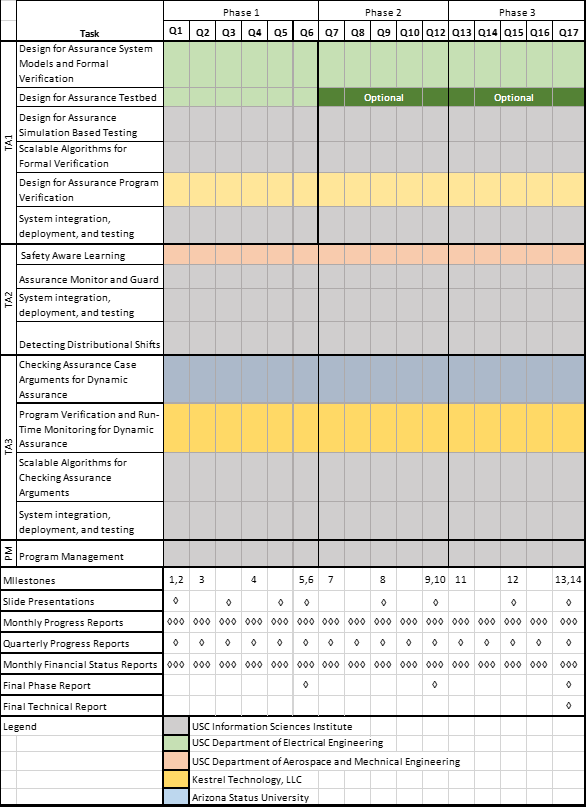
\includegraphics[width=.95\textwidth]{figs/Safeguard_Schedule_V6}
\end{center}
\vspace{-.2in}\caption{Project schedule along with a summary of milestones.  The legend maps task color to organization primary responsible for the task. } 
\label{fig:sandm}
\end{figure}
 

% \section{Level of Effort by Task \textcolor{red}{[Mike/Lisa - 1 pages]}}

% \textcolor{blue}{
% \begin{itemize}
% \item Will be a separate spreadsheet
% \item
% \end{itemize}
% }

\section*{Appendix A: Team Members and Other Information}
\addcontentsline{toc}{section}{Appendix A: Team Members and Other Information}

\baades{This section is mandatory and must include all of the following
components. If a particular subsection is not applicable, state “NONE”.}

\vspace{1ex}

\noindent
\textbf{Team Member Identification}:

\vspace{1ex}

\baades{Provide a list of all team members including the
prime, subcontractor(s), and consultant(s), as applicable. Identify specifically
whether any are a non-US organization or individual, FFRDC and/or Government
entity.}

\begin{centering}

%\small
\begin{tabular}{|p{1.8in}|p{1in}|p{1.1in}|p{0.7in}|p{0.8in}|p{0.7in}|}
\hline
 \textbf{Name} &  \textbf{Role} & \textbf{Organization} & \textbf{Non-US Org?}  & \textbf{Non-US Ind?} &  \textbf{FFRDC or Gov} \\
 \hline
Craig A. Knoblock & Prime & USC & N & N & N\\ \hline
Michael Orosz & Prime & USC & N &  N & N \\ \hline
Satish Thittamaranahalli & Prime & USC & N &  Y & N \\ \hline
Ryan Goodfellow & Prime & USC & N &  N & N \\ \hline
Anoop Kumar & Prime & USC & N & N & N \\ \hline
Satyandra Gupta & Prime & USC & N & N & N \\ \hline
Pierluigi Nuzzo & Prime & USC & N & Y & N \\ \hline
Petros Ioannou & Prime & USC & N & N & N \\ \hline
Chitta Baral & Subcontractor & ASU & N & N & N \\ \hline
Matt Barry & Subcontractor & Kestrel Technology & N & N & N \\ \hline
Douglas Smith & Subcontractor & Kestrel Technology & N & N & N \\ \hline
Henny Sipma & Subcontractor & Kestrel Technology & N & Y & N \\ \hline
\end{tabular} 
\end{centering}

\vspace{1ex}

\noindent
\textbf{Government or FFRDC Team Member Proof of Eligibility to Propose}: NONE

\baades {If
none of the team member organizations (prime or subcontractor) are a
Government entity or FFRDC, state “NONE”.}

\vspace{1ex}

\noindent
\textbf{Government or FFRDC Team Member Statement of Unique Capability}: NONE

\vspace{1ex}

\noindent
\textbf{Organizational Conflict of Interest Affirmations and Disclosure}: NONE

\vspace{1ex}

\noindent
\textbf{Intellectual Property (IP)}: 
\baades {
If no IP restrictions are intended, state “NONE”.
The Government will assume unlimited rights to all IP not explicitly identified as
having less than unlimited rights in the proposal.
For all technical data or computer software that will be furnished to the
Government with other than unlimited rights, provide (per Section VI.B.1) a list
describing all proprietary claims to results, prototypes, deliverables or systems
supporting and/or necessary for the use of the research, results, prototypes
and/or deliverables. Provide documentation proving ownership or possession of
appropriate licensing rights to all patented inventions (or inventions for which a
patent application has been filed) to be used for the proposed project.
}
\begin{centering}

%\small
\begin{tabular}{|p{2.1in}|p{1.2in}|p{1.4in}|p{2in}|}
\hline
\multicolumn{4}{|c|}{COMMERCIAL ITEMS }\\ \hline 
 \textbf{Technical Data, Computer Software To be Furnished With Restrictions} &  \textbf{Basis for Assertion} & \textbf{Asserted Rights Category} & \textbf{Name of Person Asserting Restrictions}  \\  \hline
KT Advance & Developed with mixed funding. & Restricted & David Kulich, Contracts Manager, Kestrel technology, LLC.\\ \hline
\end{tabular} 
\end{centering}

\vspace{1ex}

\noindent
\textbf{Human Subjects Research (HSR)}: NONE

\vspace{1ex}

\noindent
\textbf{Animal Use}: NONE

\vspace{1ex}

\noindent
\textbf{Representations Regarding Unpaid Delinquent Tax Liability or a Felony
Conviction under Any Federal Law}: 
%NONE

\begin{enumerate}
\item
The proposer is  not a corporation that has any unpaid Federal tax liability that has been assessed, for which all judicial and administrative remedies have been exhausted or have lapsed, and that is not being paid in a timely manner pursuant to an agreement with the authority responsible for collecting the tax liability,
\item
The proposer is not a corporation that was convicted of a felony criminal violation under a Federal law within the preceding 24 months.
\end{enumerate}

\vspace{1ex}

\noindent
\textbf{Cost Accounting Standards (CAS) Notices and Certification}:
\baades{
For any proposer who submits a proposal which, if accepted, will result in a CAS-compliant
contract, must include a Disclosure Statement as required by 48 CFR
9903.202. The disclosure forms may be found at
http://www.whitehouse.gov/omb/procurement\_casb
If this section is not applicable, state “NONE”. For further information regarding
this subject, please see www.darpa.mil/work-with-us/additional-baa.
}
NONE


%\section{Appendix B \textcolor{red}{[No Page Count]}}

\section{References}
\bibliographystyle{acm} 
\bibliography{TA3/ta3,TA2/ta2,TA1/ta1}
\end{document}
%%\documentclass[a4paper]{article}
%\documentclass[12pt]{article}
\documentclass[12pt]{dod-blank}

%% Language and font encodings
\usepackage[english]{babel}
\usepackage[utf8x]{inputenc}
\usepackage[T1]{fontenc}

%% Sets page size and margins
%%\usepackage[a4paper,top=3cm,bottom=2cm,left=3cm,right=3cm,marginparwidth=1.75cm]{geometry}
%\usepackage[top=1in, bottom=1in, left=1in, right=1in]{geometry}



%% Useful packages
\usepackage{amsmath}
\usepackage{graphicx}
  \graphicspath{{.}{./image/}}
  \DeclareGraphicsExtensions{.png,.jpg} 
\usepackage[colorinlistoftodos]{todonotes}
\usepackage[colorlinks=true, allcolors=blue]{hyperref}
\usepackage{tabularx}
\usepackage{multirow}
\usepackage{tabulary}
\usepackage{float}
\usepackage{wrapfig}
\usepackage[export]{adjustbox}
\usepackage{comment}
\usepackage{tabularx}
\usepackage{multirow}
\usepackage{tabulary}
\usepackage{enumitem}

\usepackage{listings}
\usepackage{color}
\usepackage{array}
\usepackage{subcaption}
\usepackage{xcolor}




\renewcommand{\textfraction}{0}
\renewcommand{\topfraction}{1.0}
\renewcommand{\bottomfraction}{1.0}

\usepackage{longtable}
%% macros
\newif\iffinal
\finaltrue
\iffinal
  
    \newcommand\baareq[1]{}
    \newcommand\baades[1]{}
 
 
\else
    \definecolor{darkgreen}{rgb}{0,0.4,0}
    \definecolor{darkcyan}{rgb}{0,0.4,0.4}
    \definecolor{darkblue}{rgb}{0,0,0.5}
    
    \newcommand\baareq[1]{{\color{darkcyan}[\textbf{Requirement:} #1]}}
    \newcommand\baades[1]{{\color{darkcyan}[\textbf{Description:} #1]}}
 
\fi




\def\naive{na\"{\i}ve}



\lstset{ 
  backgroundcolor=\color{white},   % choose the background color; you must add \usepackage{color} or \usepackage{xcolor}
  basicstyle=\footnotesize\ttfamily,            % the size of the fonts that are used for the code
  breakatwhitespace=false,         % sets if automatic breaks should only happen at whitespace
  breaklines=true,                 % sets automatic line breaking
  captionpos=b,                    % sets the caption-position to bottom
  commentstyle=\color{mygreen},    % comment style
  % deletekeywords={...},            % if you want to delete keywords from the given language
  escapeinside={\%*}{*)},          % if you want to add LaTeX within your code
  extendedchars=true,              % lets you use non-ASCII characters; for 8-bits encodings only, does not work with UTF-8
  frame=single,	                   % adds a frame around the code
  keepspaces=false,                 % keeps spaces in text, useful for keeping indentation of code (possibly needs columns=flexible)
  keywordstyle=\color{blue}\bfseries\underbar,       % keyword style
  language=Prolog,                 % the language of the code
  % morekeywords={if,and},        % if you want to add more keywords to the set
  numbers=none,                    % where to put the line-numbers; possible values are (none, left, right)
  numbersep=5pt,                   % how far the line-numbers are from the code
  numberstyle=\tiny\color{mygray}, % the style that is used for the line-numbers
  rulecolor=\color{black},         % if not set, the frame-color may be changed on line-breaks within not-black text
  showspaces=false,                % show spaces everywhere adding particular underscores; it overrides 'showstringspaces'
  showstringspaces=false,          % underline spaces within strings only
  showtabs=false,                  % show tabs within strings adding particular underscores
  stepnumber=2,                    % the step between two line-numbers. If it's 1, each line will be numbered
  stringstyle=\color{mymauve},     % string literal style
  tabsize=2,	                   % sets default tabsize to 2 spaces
  title=\lstname                   % show the filename of files included with \lstinputlisting; also try caption instead of title
}

% apply trick for additional keywords for our AC DSL
\lstset{
	emph={for, if, and, or},
    emphstyle={\color{blue}\bfseries\underbar}
}




\title{DARPA Assured Autonomy}
\author{Technical Volume- \textcolor{red}{Thirty-Eight (38) pages max}}

\begin{document}
\pagenumbering{roman}
 
\begin{center}
\large{\textbf{Volume 1: Technical and Management Proposal}}
\end{center}
\textbf{BAA Number:} DARPA-HR001117S0045 \\
\textbf{Technical Area:} TA1, TA2, and TA3 \\
\textbf{Proposal Title:} Assured Autonomy for Learning Enabled Vehicles (Safeguard) \\
\textbf{Lead Institution:} University of Southern California \\
\textbf{Type of organization: } “OTHER EDUCATIONAL” \\

\begin{tabularx}{\linewidth}{XX}

 \textbf{Technical Point of Contact} &  \textbf{Administrative Point of Contact }   \\
Dr.\ Craig A. Knoblock  & Sapphire Masterson  \\ 
USC Information Sciences Institute & USC Dept. of Contracts \& Grants \\
4676 Admiralty Way, Suite 1001 & 4676 Admiralty Way, Suite 1001 \\
Marina del Rey, CA 90292 & Marina del Rey, CA 90292 \\
Tel: 310-448-8786 &  Tel: (310) 448-9161 \\
E-mail: knoblock@isi.edu  & E-mail: sapphirm@usc.edu \\
\end{tabularx}
\\
\\
\textbf{Award instrument requested:}  Procurement Contract, Cost-Reimbursement, No Fee
\\
\\
\textbf{Total amount of the proposed effort:} \$ ...\\
Phase I: \$ ... \\
Phase II: \$ ... \\
Phase III: \$ ... \\
\\
\textbf{Place(s) of performance:} USC, Marina del Rey, CA; Los Angeles, CA;  Tempe, AZ; Palo Alto, CA \\
\textbf{Period(s) of performance:} 04/02/2018 - 03/31/2022     \\
\\
\textbf{Other team members:} \\
\begin{tabularx}{\linewidth}{XX}
Kestrel Technology  & Arizona State University \\
(small business) & (Other Educational)\\
POC: Matthew Barry & POC: Chitta Baral\\
3260 Hillview Avenue & Department of Computer Science and Engr. \\
Palo Alto, CA 94304 & Ira A. Fulton School of Engineering \\ 
phone: (832)205-4876 & Arizona State University\\ 
mrbarry@kestreltechnology.com & Brickyard Suite 572, 699 S. Mill Avenue \\
& Tempe, AZ 85281-8809, U.S.A.\\
& email: chitta@asu.edu\\
\end{tabularx}
\\
\textbf{Proposal validity period: } 180 days\\
\\
\textbf{Data Universal Numbering System (DUNS) number: } 072933393\\
\textbf{Taxpayer identification number:} 95-1642394\\
\textbf{Commercial and Government Entity (CAGE) code:} 1B729 Marina del Rey, CA\\
\textbf{Proposer’s reference number (if any):}  4409-0\\

\newpage
\section{Table of Contents}
\tableofcontents

\newpage
\pagenumbering{arabic}
\section{Executive Summary}
As we rapidly move into a world where machine learning plays a central role in realizing autonomous systems, it is becoming increasingly important to develop techniques that assure that these systems will operate safely and perform as expected. Current approaches are limited to providing assurance for systems with limited or no  learning capabilities. In this context, DARPA's Assured Autonomy BAA seeks to \emph{develop rigorous design and analysis technologies for continual assurance of learning-enabled autonomous systems}. USC in collaboration with Kestrel Technology and ASU is pleased to submit a comprehensive TA1, TA2, and TA3 proposal entitled \emph{``Assured Autonomy for Learning Enabled Vehicles (Safeguard).''} We plan to provide an end-to-end solution to support autonomous systems with learning-enabled components, ranging from design technologies for assurance, to assurance monitoring and control techniques, to representation and online evaluation of assurance cases. We have assembled a strong team of experts that cover the range of technologies that are required to create such an end-to-end system. If successful, the project will provide the technologies for building the next-generation of learning-enabled autonomous systems.  The entire project will take four years and cost \textcolor{red}{\$??}, with an initial version completed at the end of Phase I and successive versions with additional capabilities and improved scalability at the end of Phase II and Phase III.  

In the remainder of this section, we first introduce an  unmanned surface vehicle scenario that will be used throughout the proposal to describe the approach.  Next, we describe our approach to design, monitoring, and dynamic assurance. Finally, we introduce the team involved in the project. 

\textbf{Motivating Scenario.} Consider an autonomous unmanned surface vehicle (USV) guarding a valuable asset in the ocean when an unknown vehicle  approaches the security perimeter, under challenging weather conditions. In this scenario, the USV is required to approach the intruding vehicle, issue a warning signal, and escort it to a safe distance from the controlled area. However, as the USV has no a priori knowledge of its external environment behaviors (e.g., water depth, waves, wind, current, visibility), pre-computing a feasible trajectory, let alone optimal, becomes a non-trivial problem. For trajectory planning, the USV must continuously perform the following tasks:
\begin{itemize}[itemsep=0pt,leftmargin=*]
 \item Sense the current state of the surrounding environment (e.g., water depth, waves, wind, current, visibility) and estimate its own maneuverability constraints (e.g., braking distance, available acceleration, maximum velocity, turning radius, turning rate, safety distance) based on the state of the environment;      
\item Sense the static obstacles in the sensor range and generate a traversability map;
\item Sense the moving obstacles and classify them;   
\item Predict future trajectories of moving obstacles; 
\item Determine if any of the COLREGS \cite{commandant1999international} rules will be in effect with respect to one or more of the nearby vessels and identify the vessels with the right of way.    
\end{itemize}
The above information will be used by the trajectory planner to compute an initial trajectory, which will be continuously refined as the USV gathers additional information.
% It is not possible for the USV to be tested in every possible environment. 
The USV will use learning enabled components to take  decisions as it encounters new situations, such as  
\begin{itemize}[itemsep=0pt,leftmargin=*]
\item Classifiers to identify moving obstacles based on physical appearance and motion signatures,
\item Algorithms to estimate the sensor capabilities in adverse weather conditions,   
\item Algorithms to accurately estimate uncertainty in the environment, 
\item Classifiers to generate traversability maps,
\item Prediction of external vessel behaviors based on motion histories, 
\item Reinforcement learning  to ensure COLREGS compliance of maneuvers,  
\item Algorithms to learning pursuit behaviors.  
\end{itemize}
Learning enabled components will interact with each other in complex ways, where a misclassification error in one component may eventually compromise the entire mission.   
% We will need to make sure that each learning enabled components has a run-time monitor that will ensure that the assumptions made by the learning-enabled component remain valid and prevent erroneous learning. 
% For example, if the vehicle is exhibiting significant error in trajectory tracking, then simply downgrading the trajectory tracking error value may not be a good option.  The failure of prediction of trajectory tracking error might be due to the presence of a significant wake caused by a nearby vessel. The presence of the nearby vessel can be used to explain the degradation in trajectory tracking performance. As the vessel moves away, we can expect the trajectory tracking performance to return to the predicted level.  
While exhaustive validation of learning-enabled cyber-physical systems (LE-CPSs) is a prohibitive task~\cite{Kalra16},
their complexity, heterogeneity, and highly dynamic nature
make it challenging to even leverage existing model-based development techniques to effectively assess system correctness 
% dependability, 
at design time or enforce it at runtime.

\textbf{Design for Assurance.} Safeguard uses a platform-based design approach~\cite{Nuzzo15b} to organize the design process for a LE-CPS and to build assurance cases. Composite models are developed at several levels of abstraction,
from top-level system requirements and safety constraints down to the
implementation level.  Intermediate levels add detail to the levels
above.  The different levels are connected by refinement mappings that
allow properties established at one level to be preserved at the next
level (see Figures~\ref{fig:methodology} and~\ref{fig:assurance}).

Contracts are used to formally specify components and composite models
in terms of (1) Assumptions -- the assumed behaviors of the
environment and the behaviors of other components, and (2) Guarantees
-- the behavior properties that a model guarantees if it operates in a
context that satisfies its assumptions.  A calculus of contracts
allows horizontal composition of contracts to generate contracts for
composite models.  Vertical contracts are used to specify the mapping
or refinement relation between models at different levels of
abstraction.  The system design process starts with a high-level
contract that expresses overall system assumptions and requirements.
Subsequent levels express models with increasing detail until the
lowest level expresses the system in terms of hardware components and
their software controllers.

The assurance case for a CPS arises from the horizontal and vertical
structure of the design in several ways.  The components used within a
particular level are either (1) synthesized using
correct-by-construction design tools together with proofs, (2) derived
statically or dynamically using safety-aware machine-learning
techniques, (3) written manually and verified by analysis tools, or
(4) written manually and validated by extensive testing.  The
assurance case for the whole reflects its compositional structure.  We
anticipate that well-specified contracts together with the calculus of
contracts will eliminate well-known problems with unexpected emergent
behaviors in CPS systems.

The assurance case for the lowest-layer design arises from both the
intra-level assurance and from properties and their proofs that are
preserved under the refinement mapping from the top-level
requirements.  The refinement mappings between model layers will be
constructed using a variety of techniques.  A contract at an abstract
level can be mapped to a component or refined contract by (1)
retrieval of pre-verified components from a platform library, (2)
synthesis using correct-by-construction design and optimization tools,
or (3) manual coding to satisfy a contract.  The mapping of a
composite model will be composed from the mappings of its constituent
components or contracts.  When a composite model cannot be mapped
compositionally to the next level, it will be generated using
correct-by-construction design and optimization tools.

\textbf{Assurance Monitoring and Control.}
We provide an integrated framework for safety-aware learning, assurance monitoring and control, detecting distribution shifts. Three major components offer an efficient TA2 architecture as well as interfaces with TA1 and TA3, that is, (a) safety-aware learning and planning, (b) assurance monitors for guarding architectural and safety constraints; and (c) distribution shift detection.

We will develop a new learning-enabled online decision-making framework that allows opportunistically composing a sequence of actions (maneuvers) to reduce uncertainty in the system capability model without suspending the progress toward the mission goals or compromising safety. Each candidate action is evaluated based on three criteria: (1) the risk of violating a safety constraint using the current uncertainties in the parameter estimates; (2) its relevance to the mission goals; (3)  its expected information gain, i.e., reduction in uncertainty, with respect to the parameter estimates. These evaluations are combined to produce a cumulative mission utility value for each action that drives our learning-enabled decision-making framework. The problem of generating and evaluating sequences of actions can be posed in several way. For example, it can be solved using a branch-and-bound search method like Anytime A*, or formulated with the finite-horizon Markov Decision Process (MDP) framework. We will develop new scalable search strategies to solve this problem efficiently, by potentially evaluating a recent method developed at USC, called FastMap, that can significantly improve the execution time. 

We will develop monitors for architectural and safety constraints. 
% While these constraints can be checked over and over again as sensor information flow in, this naive strategy accounts for a lot of computational overhead. 
To achieve scalability and decrease the overhead, we propose the application of a technique that we currently use in DARPA's RSPACE program, which leverages a physical model of the vehicles dynamics and its interactions with the environment to efficiently determine the readout frequency. We propose two  extensions of this basic idea. First, we will use the theory of Variable Elimination to prioritize which variables to monitor, e.g., controllable, versus uncontrollable, adversarially controlled, or unobservable variables. Second, we invoke the dynamic assessment of assurance cases only when needed. This  decreases the number of times dynamic assessment of assurance cases is initiated as well as the communication bandwidth between the TA2 and TA3 components.

Finally, we will identify a distribution shift by combining statistical and machine learning techniques to differentiate between environmental and sensor changes. We will exploit a categorization of the shifts based on their cause and duration as well as extend our earlier work on detecting and mitigating sensor failures for all types of monitored variables.  

\textbf{Dynamic Assurance:} The Safeguard {\em design for assurance\/} activity takes a systems-theoretic stance toward safety.  Consequently, it presumes that safety is an emergent property of the system, and that hazards can present themselves through unintended interactions and performance violations in addition to causal events such as component failures.  Our design approach includes consideration of intent as well as hazard analysis and mitigation.  The artifacts from these activities populate contracts and assumptions for the dynamic assurance case.  
We thus build safety into the product by working at a systems-level viewpoint, using lexicon and design patterns familiar to both hardware and software engineers; safety is an emergent property of the system, not an afterthought.  
As system behavior evolves during runtime owing to learning, threats, degradation, or some other factor, the dynamic assurance case identifies whether the safety constraints continue to be satisfied.  If not, it provides notifications or issues recovery instructions directly from a lookup table.

Our implementation of the dynamic assurance case employs a declarative knowledge base inference engine and a domain-specific language tailored to our approach.  We have used them successfully for assurance case tool sets and arguments, and will extend them to reason about uncertainty and learning.  Our approach to achieve scalability is to specialize solvers toward modularity and to take advantage of domain knowledge.  Specifically, we will develop answer set programming techniques for context-dependent learning for reasoning about the learning-enabled components as well as learning assurance rules.  We will develop new formalisms for uncertainty to include causality, using weights for computing probabilities, and probabilistic non-monotonicity.  To achieve scaling objectives we will implement specializations using modularity, weighted CSPs, and message passing. 

% The system safety constraints revealed from that design become the key elements of our dynamic assurance case.  Our verification tools ensure the constraints are relevant, identifiable, and their implementation and effect observable.  

\textbf{Team.} We have assembled a team that is exceptionally well-qualified to build the proposed Safeguard system.  The team will be led by Dr.\ Craig Knoblock, the Principal Investigator for the effort, who currently leads the Intelligent Systems Division at the Information Sciences Institute.  He has led many large DARPA and IARPA projects over the years and has a strong track record in conducting leading edge research and then transitioning the technology to commercial use.  He will be supported by Dr.\ Michael Orosz as the Project Manager, who also has  experience in managing large research projects and on autonomous systems.  The TA1 team will be led by Dr.\ Pierluigi Nuzzo, who is an expert in embedded system design methodologies and the  application of formal methods to cyber-physical systems.  The TA1 team also includes Dr.\ Doug Smith, who has spent many years working on scalable correct-by-construction techniques and Dr.\ Henny Sipma, who has significant experience in applying program verification methods to real-world problems.  The TA1 team also includes Ryan Goodfellow, who has done a large amount of work on simulation-based testing.  The TA2 team will be led by Dr.\ Knoblock who has worked on topics related to both monitoring and detecting distribution changes.  He will be supported by Dr.\ Satyandra Gupta, who is an expert on autonomous surface vehicles as well as on safety-aware learning. He will also be supported by Drs.\ Anoop Kumar and Satish Thittamaranahalli, who have also previously worked on efficient methods for execution monitoring.  The TA3 team will be lead by Dr.\ Matthew Barry, who has experience in creating the technologies for assurance cases.  He will be supported by Dr.\ Chitta Baral, who is an expert on ASP solvers and by Dr.\ Thittamaranahalli who is an expert on SAT solvers, both of which will be applied to provide scalable assurance case reasoning.  Finally, Dr.\ Petros Ioannou, who is an expert on control systems for autonomous vehicles will provide an autonomous vehicle platform, which will form the focus of our work until the TA4 teams provide additional vehicle platforms for development.  

\newpage
\section{Innovative Claims and Deliverables}

In this project we will develop and build an end-to-end system for assured autonomy.  This section describes the key innovations by technical area and then the overall deliverables of the project.

\paragraph{Design for Assurance}

\begin{itemize}[itemsep=0pt,leftmargin=*]
\item We address the LE-CPS design challenges via a holistic approach that can contextually generate design artifacts and assurance cases. We develop a compositional, contract-based modeling framework, methods, and tools to support the design process from system-level requirement capture,  formalization, and analysis, to the generation, testing, and continual monitoring of software and hardware artifacts in feedback loop with a physical process.

\item We develop compositional abstractions and interfaces (vertical contracts) that can  bridge heterogeneous formalisms and heterogeneous decomposition architectures to make system analysis and synthesis tractable, consistently combine different verification and synthesis methods at design time, and provide seamless support for dynamic assurance at run time. %We aim to quantitatively capture the confidence in the satisfaction of requirements under uncertain or unknown conditions, and resilience properties of  systems at different abstraction levels, to enable trade-off evaluation between resilience, performance, and cost.

\item We develop a unifying framework and efficient algorithms to reason about the combination of discrete and continuous dynamics and constraints in the presence of uncertainties in LE-CPS using a satisfiability modulo convex approach~\cite{Shoukry2017} for contract-based system verification and scalable trajectory planning.  

\item We provide an environment for high-fidelity CPS testing, in which production-ready software, e.g.,  safety-critical learning and control, may be deployed and tested 
% by extending the Cypress testbed environment \cite{Goodfellow2015Cypress:Systems} 
with time dilation facilities, so that it synchronizes with a physical simulation that is not necessarily running in real time, while still having the perception of real time.

\item We 
% These facilities allow a cyber system to be  
propose an approach for unanticipated behavior space identification and test coverage maximization which leverages results from the theory of differential algebraic equation (DAE)~\cite{Berger2013ControllabilitySurvey,Ilchmann2005ATheory,BergerOnSystems,Lamour2013} 
to prune the behavior search space and identify smaller regions of interest for efficient simulation-based testing. 
% We then compute the intersection of these two behavior spaces and restrict our simulation based testing search space to this subspace.
\end{itemize}

\paragraph{Assurance Monitoring and Control}

\begin{itemize}[itemsep=0pt,leftmargin=*]
\item 
%We integrate safety-aware learning into the overall decision making problem. The goal is to maximize mission utility without violating the safety constraints. 
Our safety-aware learning framework enables the system to opportunistically select and execute actions to assist the learning-enabled component in reducing model uncertainty without compromising safety or deviating from the mission goals. The value of uncertainty reduction is explicitly incorporated in the optimization process for selecting the best action.  
\item For safety-aware learning, we propose the idea of preprocessing the search space of the problem domain before queries and observations come in. With such a linear-time preprocessing phase, the performance of search and optimization algorithms can be significantly boosted. For example, in regular A* search, the intensional or extensional search space can be preprocessed in near-linear time to yield an embedding of each state as a point in Euclidean space~\cite{cujakk}. Then, when the query comes in, A* search can make use of these Euclidean distances as heuristic distances between two states to yield order-of-magnitude speedups. 
%In Anytime A* for safety-aware learning and planning, this leads to a significantly better quality of actions chosen within a time limit, and in the MDP framework, the same ideas can be used to improve the convergence of Bellman updates for safety-aware Reinforcement Learning.
\item As massive amounts of sensor information flow in, it is imperative for us to efficiently process this information for monitoring architectural and safety constraints. Building on our past work on similar tasks, we propose novel technologies for efficiently monitoring constraints. These algorithms can yield an exponential reduction in the amount of sensor data that needs to be processed. Doing this also reduces the message complexities between the various modules. %We also propose to use the theory of Variable Elimination (VE) to monitor constraints with uncontrollable, adversarially controlled, and/or unobservable variables. VE yields a substrate constraint to monitor that characterizes a dominant strategy of the controllable variables over the uncontrollable, adversarially controlled, and/or unobservable variables.
\item We will develop techniques to identify  distributional shifts and determine the underlying cause (e.g., change in environment, sensor failure,   etc.), as well as strategies for handling the various distributional shifts.   Notably, we propose to build on our past work and use compact representations to exploit historical data to identify distributional shifts.
\end{itemize}

\paragraph{Dynamic Assurance}

\begin{itemize}[itemsep=0pt,leftmargin=*]

\item We demonstrate the integration of dynamic assurance for safety-critical learning-enabled dynamic systems in which evolutionary behaviors are expected and tolerated as a property of the functionality.   The impact will be consequential contributions safety-critical dynamic systems in which evolutionary behaviors are expected and tolerated as portion of the functionality.   
\item We implement dynamic assurance by combining features of system safety, formal methods, logic programming, uncertain reasoning, and domain-specific languages.  We populate assurance case arguments at several levels of modeling and implementation abstraction, using the analysis results to produce design-time evidence supporting assurance claims.  
%We provide automated reasoning about the assurance case itself to produce verification, consistency, and completeness results for the argument.  Dynamic assurance results then yield trusted explanations of whether safety constraints and assumptions and other contracts still hold during the collection of runtime evidence from monitors. 
\item We develop and demonstrate ASP formalisms crucial to applications in dynamic assurance. We demonstrate the suitability of the technology especially for assurance case arguments owing to the improved legibility, consistency and completeness checks, handling of uncertain and default reasoning, and scalability.  
%We will produce modularized solvers for enhanced performance based on recent algorithmic developments in exploiting structure, kernelization, and message passing. We provide a formalism to enable learning of assurance rules. 
We provide a novel approach to handling uncertainty that provides the ability to do causal and counter-factual reasoning as well as probabilistic non-monotonicity.  Overcoming limitations of traditional inductive logic techniques, we develop a novel iterative and incremental approach based on context dependent learning. 
\end{itemize}

\paragraph{Deliverables}
During the course of this project, we will build and deliver a fully-operational system that covers all three of the technical areas.  The detailed capabilities of this system are described in the individual technical sections.  The resulting system will be available as open source under a permissive license, which will allow other organizations to use the work, extend it in new directions, and even commercialize the software.  Kestrel Technology has significant experience in this space and has built and applied these types of technologies to a variety of real world tasks.  Kestrel is ideally suited to pursue commercial uses of this technology and the permissive license will facilitate exploring these opportunities since there will be no need to negotiate intellectual property rights.  

\newpage
\section{Technical Plan}
%%\documentclass[a4paper]{article}
%\documentclass[12pt]{article}
\documentclass[12pt]{dod-blank}

%% Language and font encodings
\usepackage[english]{babel}
\usepackage[utf8x]{inputenc}
\usepackage[T1]{fontenc}

%% Sets page size and margins
%%\usepackage[a4paper,top=3cm,bottom=2cm,left=3cm,right=3cm,marginparwidth=1.75cm]{geometry}
%\usepackage[top=1in, bottom=1in, left=1in, right=1in]{geometry}



%% Useful packages
\usepackage{amsmath}
\usepackage{graphicx}
  \graphicspath{{.}{./image/}}
  \DeclareGraphicsExtensions{.png,.jpg} 
\usepackage[colorinlistoftodos]{todonotes}
\usepackage[colorlinks=true, allcolors=blue]{hyperref}
\usepackage{tabularx}
\usepackage{multirow}
\usepackage{tabulary}
\usepackage{float}
\usepackage{wrapfig}
\usepackage[export]{adjustbox}
\usepackage{comment}
\usepackage{tabularx}
\usepackage{multirow}
\usepackage{tabulary}
\usepackage{enumitem}

\usepackage{listings}
\usepackage{color}
\usepackage{array}
\usepackage{subcaption}
\usepackage{xcolor}




\renewcommand{\textfraction}{0}
\renewcommand{\topfraction}{1.0}
\renewcommand{\bottomfraction}{1.0}

\usepackage{longtable}
%% macros
\newif\iffinal
\finaltrue
\iffinal
  
    \newcommand\baareq[1]{}
    \newcommand\baades[1]{}
 
 
\else
    \definecolor{darkgreen}{rgb}{0,0.4,0}
    \definecolor{darkcyan}{rgb}{0,0.4,0.4}
    \definecolor{darkblue}{rgb}{0,0,0.5}
    
    \newcommand\baareq[1]{{\color{darkcyan}[\textbf{Requirement:} #1]}}
    \newcommand\baades[1]{{\color{darkcyan}[\textbf{Description:} #1]}}
 
\fi




\def\naive{na\"{\i}ve}



\lstset{ 
  backgroundcolor=\color{white},   % choose the background color; you must add \usepackage{color} or \usepackage{xcolor}
  basicstyle=\footnotesize\ttfamily,            % the size of the fonts that are used for the code
  breakatwhitespace=false,         % sets if automatic breaks should only happen at whitespace
  breaklines=true,                 % sets automatic line breaking
  captionpos=b,                    % sets the caption-position to bottom
  commentstyle=\color{mygreen},    % comment style
  % deletekeywords={...},            % if you want to delete keywords from the given language
  escapeinside={\%*}{*)},          % if you want to add LaTeX within your code
  extendedchars=true,              % lets you use non-ASCII characters; for 8-bits encodings only, does not work with UTF-8
  frame=single,	                   % adds a frame around the code
  keepspaces=false,                 % keeps spaces in text, useful for keeping indentation of code (possibly needs columns=flexible)
  keywordstyle=\color{blue}\bfseries\underbar,       % keyword style
  language=Prolog,                 % the language of the code
  % morekeywords={if,and},        % if you want to add more keywords to the set
  numbers=none,                    % where to put the line-numbers; possible values are (none, left, right)
  numbersep=5pt,                   % how far the line-numbers are from the code
  numberstyle=\tiny\color{mygray}, % the style that is used for the line-numbers
  rulecolor=\color{black},         % if not set, the frame-color may be changed on line-breaks within not-black text
  showspaces=false,                % show spaces everywhere adding particular underscores; it overrides 'showstringspaces'
  showstringspaces=false,          % underline spaces within strings only
  showtabs=false,                  % show tabs within strings adding particular underscores
  stepnumber=2,                    % the step between two line-numbers. If it's 1, each line will be numbered
  stringstyle=\color{mymauve},     % string literal style
  tabsize=2,	                   % sets default tabsize to 2 spaces
  title=\lstname                   % show the filename of files included with \lstinputlisting; also try caption instead of title
}

% apply trick for additional keywords for our AC DSL
\lstset{
	emph={for, if, and, or},
    emphstyle={\color{blue}\bfseries\underbar}
}




\title{DARPA Assured Autonomy}
\author{Technical Volume- \textcolor{red}{Thirty-Eight (38) pages max}}

\begin{document}
\pagenumbering{roman}
\include{cover}

\newpage
\section{Table of Contents}
\tableofcontents

\newpage
\pagenumbering{arabic}
\section{Executive Summary}
As we rapidly move into a world where machine learning plays a central role in realizing autonomous systems, it is becoming increasingly important to develop techniques that assure that these systems will operate safely and perform as expected. Current approaches are limited to providing assurance for systems with limited or no  learning capabilities. In this context, DARPA's Assured Autonomy BAA seeks to \emph{develop rigorous design and analysis technologies for continual assurance of learning-enabled autonomous systems}. USC in collaboration with Kestrel Technology and ASU is pleased to submit a comprehensive TA1, TA2, and TA3 proposal entitled \emph{``Assured Autonomy for Learning Enabled Vehicles (Safeguard).''} We plan to provide an end-to-end solution to support autonomous systems with learning-enabled components, ranging from design technologies for assurance, to assurance monitoring and control techniques, to representation and online evaluation of assurance cases. We have assembled a strong team of experts that cover the range of technologies that are required to create such an end-to-end system. If successful, the project will provide the technologies for building the next-generation of learning-enabled autonomous systems.  The entire project will take four years and cost \textcolor{red}{\$??}, with an initial version completed at the end of Phase I and successive versions with additional capabilities and improved scalability at the end of Phase II and Phase III.  

In the remainder of this section, we first introduce an  unmanned surface vehicle scenario that will be used throughout the proposal to describe the approach.  Next, we describe our approach to design, monitoring, and dynamic assurance. Finally, we introduce the team involved in the project. 

\textbf{Motivating Scenario.} Consider an autonomous unmanned surface vehicle (USV) guarding a valuable asset in the ocean when an unknown vehicle  approaches the security perimeter, under challenging weather conditions. In this scenario, the USV is required to approach the intruding vehicle, issue a warning signal, and escort it to a safe distance from the controlled area. However, as the USV has no a priori knowledge of its external environment behaviors (e.g., water depth, waves, wind, current, visibility), pre-computing a feasible trajectory, let alone optimal, becomes a non-trivial problem. For trajectory planning, the USV must continuously perform the following tasks:
\begin{itemize}[itemsep=0pt,leftmargin=*]
 \item Sense the current state of the surrounding environment (e.g., water depth, waves, wind, current, visibility) and estimate its own maneuverability constraints (e.g., braking distance, available acceleration, maximum velocity, turning radius, turning rate, safety distance) based on the state of the environment;      
\item Sense the static obstacles in the sensor range and generate a traversability map;
\item Sense the moving obstacles and classify them;   
\item Predict future trajectories of moving obstacles; 
\item Determine if any of the COLREGS \cite{commandant1999international} rules will be in effect with respect to one or more of the nearby vessels and identify the vessels with the right of way.    
\end{itemize}
The above information will be used by the trajectory planner to compute an initial trajectory, which will be continuously refined as the USV gathers additional information.
% It is not possible for the USV to be tested in every possible environment. 
The USV will use learning enabled components to take  decisions as it encounters new situations, such as  
\begin{itemize}[itemsep=0pt,leftmargin=*]
\item Classifiers to identify moving obstacles based on physical appearance and motion signatures,
\item Algorithms to estimate the sensor capabilities in adverse weather conditions,   
\item Algorithms to accurately estimate uncertainty in the environment, 
\item Classifiers to generate traversability maps,
\item Prediction of external vessel behaviors based on motion histories, 
\item Reinforcement learning  to ensure COLREGS compliance of maneuvers,  
\item Algorithms to learning pursuit behaviors.  
\end{itemize}
Learning enabled components will interact with each other in complex ways, where a misclassification error in one component may eventually compromise the entire mission.   
% We will need to make sure that each learning enabled components has a run-time monitor that will ensure that the assumptions made by the learning-enabled component remain valid and prevent erroneous learning. 
% For example, if the vehicle is exhibiting significant error in trajectory tracking, then simply downgrading the trajectory tracking error value may not be a good option.  The failure of prediction of trajectory tracking error might be due to the presence of a significant wake caused by a nearby vessel. The presence of the nearby vessel can be used to explain the degradation in trajectory tracking performance. As the vessel moves away, we can expect the trajectory tracking performance to return to the predicted level.  
While exhaustive validation of learning-enabled cyber-physical systems (LE-CPSs) is a prohibitive task~\cite{Kalra16},
their complexity, heterogeneity, and highly dynamic nature
make it challenging to even leverage existing model-based development techniques to effectively assess system correctness 
% dependability, 
at design time or enforce it at runtime.

\textbf{Design for Assurance.} Safeguard uses a platform-based design approach~\cite{Nuzzo15b} to organize the design process for a LE-CPS and to build assurance cases. Composite models are developed at several levels of abstraction,
from top-level system requirements and safety constraints down to the
implementation level.  Intermediate levels add detail to the levels
above.  The different levels are connected by refinement mappings that
allow properties established at one level to be preserved at the next
level (see Figures~\ref{fig:methodology} and~\ref{fig:assurance}).

Contracts are used to formally specify components and composite models
in terms of (1) Assumptions -- the assumed behaviors of the
environment and the behaviors of other components, and (2) Guarantees
-- the behavior properties that a model guarantees if it operates in a
context that satisfies its assumptions.  A calculus of contracts
allows horizontal composition of contracts to generate contracts for
composite models.  Vertical contracts are used to specify the mapping
or refinement relation between models at different levels of
abstraction.  The system design process starts with a high-level
contract that expresses overall system assumptions and requirements.
Subsequent levels express models with increasing detail until the
lowest level expresses the system in terms of hardware components and
their software controllers.

The assurance case for a CPS arises from the horizontal and vertical
structure of the design in several ways.  The components used within a
particular level are either (1) synthesized using
correct-by-construction design tools together with proofs, (2) derived
statically or dynamically using safety-aware machine-learning
techniques, (3) written manually and verified by analysis tools, or
(4) written manually and validated by extensive testing.  The
assurance case for the whole reflects its compositional structure.  We
anticipate that well-specified contracts together with the calculus of
contracts will eliminate well-known problems with unexpected emergent
behaviors in CPS systems.

The assurance case for the lowest-layer design arises from both the
intra-level assurance and from properties and their proofs that are
preserved under the refinement mapping from the top-level
requirements.  The refinement mappings between model layers will be
constructed using a variety of techniques.  A contract at an abstract
level can be mapped to a component or refined contract by (1)
retrieval of pre-verified components from a platform library, (2)
synthesis using correct-by-construction design and optimization tools,
or (3) manual coding to satisfy a contract.  The mapping of a
composite model will be composed from the mappings of its constituent
components or contracts.  When a composite model cannot be mapped
compositionally to the next level, it will be generated using
correct-by-construction design and optimization tools.

\textbf{Assurance Monitoring and Control.}
We provide an integrated framework for safety-aware learning, assurance monitoring and control, detecting distribution shifts. Three major components offer an efficient TA2 architecture as well as interfaces with TA1 and TA3, that is, (a) safety-aware learning and planning, (b) assurance monitors for guarding architectural and safety constraints; and (c) distribution shift detection.

We will develop a new learning-enabled online decision-making framework that allows opportunistically composing a sequence of actions (maneuvers) to reduce uncertainty in the system capability model without suspending the progress toward the mission goals or compromising safety. Each candidate action is evaluated based on three criteria: (1) the risk of violating a safety constraint using the current uncertainties in the parameter estimates; (2) its relevance to the mission goals; (3)  its expected information gain, i.e., reduction in uncertainty, with respect to the parameter estimates. These evaluations are combined to produce a cumulative mission utility value for each action that drives our learning-enabled decision-making framework. The problem of generating and evaluating sequences of actions can be posed in several way. For example, it can be solved using a branch-and-bound search method like Anytime A*, or formulated with the finite-horizon Markov Decision Process (MDP) framework. We will develop new scalable search strategies to solve this problem efficiently, by potentially evaluating a recent method developed at USC, called FastMap, that can significantly improve the execution time. 

We will develop monitors for architectural and safety constraints. 
% While these constraints can be checked over and over again as sensor information flow in, this naive strategy accounts for a lot of computational overhead. 
To achieve scalability and decrease the overhead, we propose the application of a technique that we currently use in DARPA's RSPACE program, which leverages a physical model of the vehicles dynamics and its interactions with the environment to efficiently determine the readout frequency. We propose two  extensions of this basic idea. First, we will use the theory of Variable Elimination to prioritize which variables to monitor, e.g., controllable, versus uncontrollable, adversarially controlled, or unobservable variables. Second, we invoke the dynamic assessment of assurance cases only when needed. This  decreases the number of times dynamic assessment of assurance cases is initiated as well as the communication bandwidth between the TA2 and TA3 components.

Finally, we will identify a distribution shift by combining statistical and machine learning techniques to differentiate between environmental and sensor changes. We will exploit a categorization of the shifts based on their cause and duration as well as extend our earlier work on detecting and mitigating sensor failures for all types of monitored variables.  

\textbf{Dynamic Assurance:} The Safeguard {\em design for assurance\/} activity takes a systems-theoretic stance toward safety.  Consequently, it presumes that safety is an emergent property of the system, and that hazards can present themselves through unintended interactions and performance violations in addition to causal events such as component failures.  Our design approach includes consideration of intent as well as hazard analysis and mitigation.  The artifacts from these activities populate contracts and assumptions for the dynamic assurance case.  
We thus build safety into the product by working at a systems-level viewpoint, using lexicon and design patterns familiar to both hardware and software engineers; safety is an emergent property of the system, not an afterthought.  
As system behavior evolves during runtime owing to learning, threats, degradation, or some other factor, the dynamic assurance case identifies whether the safety constraints continue to be satisfied.  If not, it provides notifications or issues recovery instructions directly from a lookup table.

Our implementation of the dynamic assurance case employs a declarative knowledge base inference engine and a domain-specific language tailored to our approach.  We have used them successfully for assurance case tool sets and arguments, and will extend them to reason about uncertainty and learning.  Our approach to achieve scalability is to specialize solvers toward modularity and to take advantage of domain knowledge.  Specifically, we will develop answer set programming techniques for context-dependent learning for reasoning about the learning-enabled components as well as learning assurance rules.  We will develop new formalisms for uncertainty to include causality, using weights for computing probabilities, and probabilistic non-monotonicity.  To achieve scaling objectives we will implement specializations using modularity, weighted CSPs, and message passing. 

% The system safety constraints revealed from that design become the key elements of our dynamic assurance case.  Our verification tools ensure the constraints are relevant, identifiable, and their implementation and effect observable.  

\textbf{Team.} We have assembled a team that is exceptionally well-qualified to build the proposed Safeguard system.  The team will be led by Dr.\ Craig Knoblock, the Principal Investigator for the effort, who currently leads the Intelligent Systems Division at the Information Sciences Institute.  He has led many large DARPA and IARPA projects over the years and has a strong track record in conducting leading edge research and then transitioning the technology to commercial use.  He will be supported by Dr.\ Michael Orosz as the Project Manager, who also has  experience in managing large research projects and on autonomous systems.  The TA1 team will be led by Dr.\ Pierluigi Nuzzo, who is an expert in embedded system design methodologies and the  application of formal methods to cyber-physical systems.  The TA1 team also includes Dr.\ Doug Smith, who has spent many years working on scalable correct-by-construction techniques and Dr.\ Henny Sipma, who has significant experience in applying program verification methods to real-world problems.  The TA1 team also includes Ryan Goodfellow, who has done a large amount of work on simulation-based testing.  The TA2 team will be led by Dr.\ Knoblock who has worked on topics related to both monitoring and detecting distribution changes.  He will be supported by Dr.\ Satyandra Gupta, who is an expert on autonomous surface vehicles as well as on safety-aware learning. He will also be supported by Drs.\ Anoop Kumar and Satish Thittamaranahalli, who have also previously worked on efficient methods for execution monitoring.  The TA3 team will be lead by Dr.\ Matthew Barry, who has experience in creating the technologies for assurance cases.  He will be supported by Dr.\ Chitta Baral, who is an expert on ASP solvers and by Dr.\ Thittamaranahalli who is an expert on SAT solvers, both of which will be applied to provide scalable assurance case reasoning.  Finally, Dr.\ Petros Ioannou, who is an expert on control systems for autonomous vehicles will provide an autonomous vehicle platform, which will form the focus of our work until the TA4 teams provide additional vehicle platforms for development.  

\newpage
\section{Innovative Claims and Deliverables}

In this project we will develop and build an end-to-end system for assured autonomy.  This section describes the key innovations by technical area and then the overall deliverables of the project.

\paragraph{Design for Assurance}

\begin{itemize}[itemsep=0pt,leftmargin=*]
\item We address the LE-CPS design challenges via a holistic approach that can contextually generate design artifacts and assurance cases. We develop a compositional, contract-based modeling framework, methods, and tools to support the design process from system-level requirement capture,  formalization, and analysis, to the generation, testing, and continual monitoring of software and hardware artifacts in feedback loop with a physical process.

\item We develop compositional abstractions and interfaces (vertical contracts) that can  bridge heterogeneous formalisms and heterogeneous decomposition architectures to make system analysis and synthesis tractable, consistently combine different verification and synthesis methods at design time, and provide seamless support for dynamic assurance at run time. %We aim to quantitatively capture the confidence in the satisfaction of requirements under uncertain or unknown conditions, and resilience properties of  systems at different abstraction levels, to enable trade-off evaluation between resilience, performance, and cost.

\item We develop a unifying framework and efficient algorithms to reason about the combination of discrete and continuous dynamics and constraints in the presence of uncertainties in LE-CPS using a satisfiability modulo convex approach~\cite{Shoukry2017} for contract-based system verification and scalable trajectory planning.  

\item We provide an environment for high-fidelity CPS testing, in which production-ready software, e.g.,  safety-critical learning and control, may be deployed and tested 
% by extending the Cypress testbed environment \cite{Goodfellow2015Cypress:Systems} 
with time dilation facilities, so that it synchronizes with a physical simulation that is not necessarily running in real time, while still having the perception of real time.

\item We 
% These facilities allow a cyber system to be  
propose an approach for unanticipated behavior space identification and test coverage maximization which leverages results from the theory of differential algebraic equation (DAE)~\cite{Berger2013ControllabilitySurvey,Ilchmann2005ATheory,BergerOnSystems,Lamour2013} 
to prune the behavior search space and identify smaller regions of interest for efficient simulation-based testing. 
% We then compute the intersection of these two behavior spaces and restrict our simulation based testing search space to this subspace.
\end{itemize}

\paragraph{Assurance Monitoring and Control}

\begin{itemize}[itemsep=0pt,leftmargin=*]
\item 
%We integrate safety-aware learning into the overall decision making problem. The goal is to maximize mission utility without violating the safety constraints. 
Our safety-aware learning framework enables the system to opportunistically select and execute actions to assist the learning-enabled component in reducing model uncertainty without compromising safety or deviating from the mission goals. The value of uncertainty reduction is explicitly incorporated in the optimization process for selecting the best action.  
\item For safety-aware learning, we propose the idea of preprocessing the search space of the problem domain before queries and observations come in. With such a linear-time preprocessing phase, the performance of search and optimization algorithms can be significantly boosted. For example, in regular A* search, the intensional or extensional search space can be preprocessed in near-linear time to yield an embedding of each state as a point in Euclidean space~\cite{cujakk}. Then, when the query comes in, A* search can make use of these Euclidean distances as heuristic distances between two states to yield order-of-magnitude speedups. 
%In Anytime A* for safety-aware learning and planning, this leads to a significantly better quality of actions chosen within a time limit, and in the MDP framework, the same ideas can be used to improve the convergence of Bellman updates for safety-aware Reinforcement Learning.
\item As massive amounts of sensor information flow in, it is imperative for us to efficiently process this information for monitoring architectural and safety constraints. Building on our past work on similar tasks, we propose novel technologies for efficiently monitoring constraints. These algorithms can yield an exponential reduction in the amount of sensor data that needs to be processed. Doing this also reduces the message complexities between the various modules. %We also propose to use the theory of Variable Elimination (VE) to monitor constraints with uncontrollable, adversarially controlled, and/or unobservable variables. VE yields a substrate constraint to monitor that characterizes a dominant strategy of the controllable variables over the uncontrollable, adversarially controlled, and/or unobservable variables.
\item We will develop techniques to identify  distributional shifts and determine the underlying cause (e.g., change in environment, sensor failure,   etc.), as well as strategies for handling the various distributional shifts.   Notably, we propose to build on our past work and use compact representations to exploit historical data to identify distributional shifts.
\end{itemize}

\paragraph{Dynamic Assurance}

\begin{itemize}[itemsep=0pt,leftmargin=*]

\item We demonstrate the integration of dynamic assurance for safety-critical learning-enabled dynamic systems in which evolutionary behaviors are expected and tolerated as a property of the functionality.   The impact will be consequential contributions safety-critical dynamic systems in which evolutionary behaviors are expected and tolerated as portion of the functionality.   
\item We implement dynamic assurance by combining features of system safety, formal methods, logic programming, uncertain reasoning, and domain-specific languages.  We populate assurance case arguments at several levels of modeling and implementation abstraction, using the analysis results to produce design-time evidence supporting assurance claims.  
%We provide automated reasoning about the assurance case itself to produce verification, consistency, and completeness results for the argument.  Dynamic assurance results then yield trusted explanations of whether safety constraints and assumptions and other contracts still hold during the collection of runtime evidence from monitors. 
\item We develop and demonstrate ASP formalisms crucial to applications in dynamic assurance. We demonstrate the suitability of the technology especially for assurance case arguments owing to the improved legibility, consistency and completeness checks, handling of uncertain and default reasoning, and scalability.  
%We will produce modularized solvers for enhanced performance based on recent algorithmic developments in exploiting structure, kernelization, and message passing. We provide a formalism to enable learning of assurance rules. 
We provide a novel approach to handling uncertainty that provides the ability to do causal and counter-factual reasoning as well as probabilistic non-monotonicity.  Overcoming limitations of traditional inductive logic techniques, we develop a novel iterative and incremental approach based on context dependent learning. 
\end{itemize}

\paragraph{Deliverables}
During the course of this project, we will build and deliver a fully-operational system that covers all three of the technical areas.  The detailed capabilities of this system are described in the individual technical sections.  The resulting system will be available as open source under a permissive license, which will allow other organizations to use the work, extend it in new directions, and even commercialize the software.  Kestrel Technology has significant experience in this space and has built and applied these types of technologies to a variety of real world tasks.  Kestrel is ideally suited to pursue commercial uses of this technology and the permissive license will facilitate exploring these opportunities since there will be no need to negotiate intellectual property rights.  

\newpage
\section{Technical Plan}
\input{./TA1/main}
\input{./TA2/main}
\input{./TA3/main}
\clearpage
\newpage


\section{Management Plan}


The Principal Investigator for this effort is Dr. Craig Knoblock who is responsible for all aspects of the effort, will coordinate the parallel team efforts, and will ensure high levels of performance from individual team members.  The Co-P/I, Dr. Michael Orosz, will provide project management and will assist all performers in the execution of the project.    The project team is divided into three working groups (Figure~\ref{fig:org_chart}) corresponding to Technical Areas 1-3, however, members of each team contribute across all project activities.   Table~\ref{fig:Table_Mgmt} defines the major contributions of each project team member to the project tasks.

\begin{figure}[tbhp]
%\vspace{-25pt}
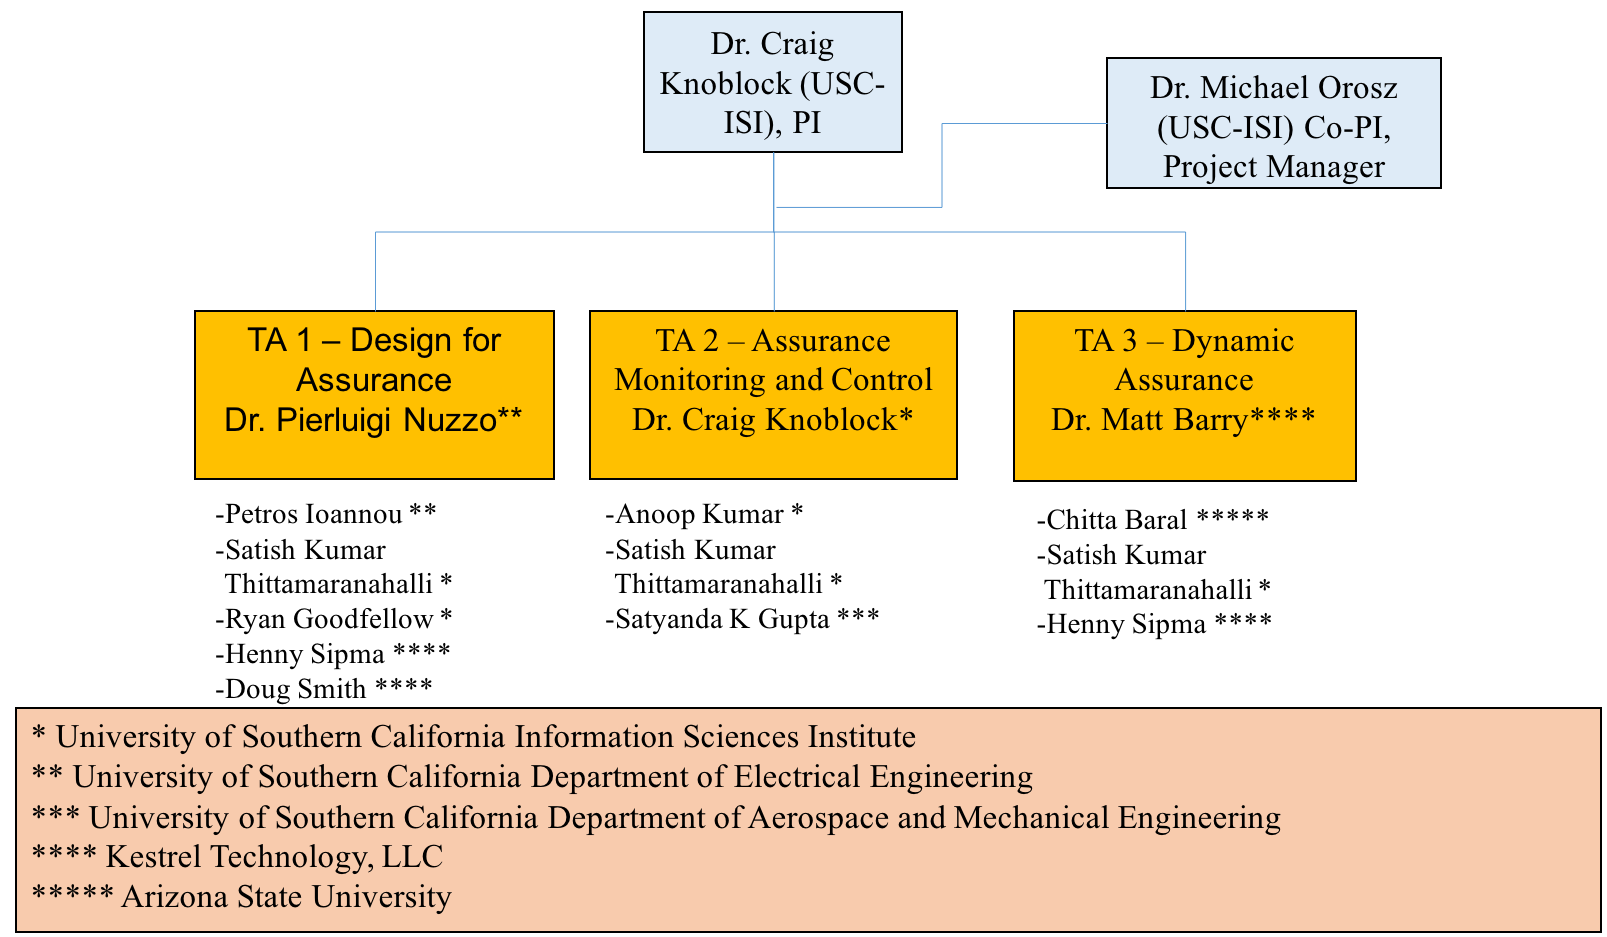
\includegraphics[width=6.0in]{./org-chart2.png}
\caption{\small Organization Chart}
\label{fig:org_chart}
\end{figure}

Coordination: To maximize collaboration and reduce risk to project failure from lack of communication and technical exchange, we plan to employ a wide variety of working styles and communication/coordination so that all can contribute.  At the core of our project will be regularly scheduled meetings bridging the diversely distributed team (Table~\ref{fig:Collaboration_Table}).  These meetings will address project status, identify challenges, implement risk mitigation strategies and participate in technology exchanges and system integration efforts (when appropriate)

\begin{table}[ht]
\caption{\small Project Meetings and Events}
  \centering
  {\footnotesize
\begin{tabular}{|m{3.15in}|m{3in}|} 
\hline
\textbf{Meeting} & \textbf{Frequency} 
\\\hline
Conference calls among investigators (discuss project status, address concerns and project risks) & Weekly
\\
\hline
Technical exchange and coordination meetings using Bluejeans or another videoconference technology & At least twice a month and more frequently as needed
  \\ 
\hline
Face-to-Face meetings (prior to P/I and demonstration meetings) & Every 3 to 6 months and more frequently (especially at the beginning of the project) as needed
 \\\cline{1-2}

\hline
\end{tabular}
}
\label{fig:Collaboration_Table}
\end{table}

\begin{table}[tbhp]
\caption{\small Key Project Team Member Responsibilities}
  \centering
  {\footnotesize
\begin{tabular}{| m{.75in} | m{3.9in}| m{1.5in}|} 
\hline
\textbf{Key Member} & \textbf{Responsibilities} & \textbf{Tasks} 
\\\hline
Dr.\ Craig Knoblock  & Principal Investigator responsible for project, leads TA 2 – Assurance Monitoring and Control.  Will lead the overall project and lead the TA2 team.  Served as the PI on many DARPA projects and has sucessfully led many large teams.    Effort on project:  25\% &
1.1.6, 1.2.2 1.2.3, 1.2.4, 1.3.4, 1.4.1, 
2.1.6, 2.2.2 2.2.3, 2.2.4, 2.3.4, 2.4.1, 
3.1.6, 3.2.2, 3.2.3, 3.2.4, 3.3.4, 3.4.1
\\
\hline
Dr.\ Michael Orosz & Co-Principal Investigator responsible managing the day-to-day operations of the project, assist technical teams as needed, coordinate with TA4 teams.    Has led many large complex multi-disciplined/multi-organizational projects in academic and industry environments.  Effort on project: 50\%
& 1.1.6, 2.1.6, 3.1.6, 1.4.1, 2.4.1, 3.4.1
  \\ 
\hline
Dr.\ Pierluigi Nuzzo 
& 
Co-Principal Investigator.  Leads the TA 1 - Design for Assurance team and conducts research on the formal methods for the design of the TA1 system.  Research experience on methodologies and tools for the design of cyber-physical systems; contracts, interfaces, and compositional methods for embedded system design; the application of automated formal methods and optimization theory to problems in embedded and cyber-physical systems.  Effort on project: 2 months/year (16.6\%)
& 
1.1.1, 2.1.1, 3.1.1 \\
\hline
Dr.\ Matthew Barry
& 
Key personnel.  Leads the TA 3 – Dynamic Assurance.   He will conduct the research on the dynamic assurance case language editors and parsers, the run-time system, and system integrations. Effort on project:  66\%
& 
1.3.2, 2.3.2, 3.3.2\\
\hline
Dr.\ Chitta Baral
& 
Key personnel responsible for learning assurance rules, supporting assurance rules with uncertainty and improving solver speed.  Expertise on ASP solvers, which will be used to reason about the assurance cases. Effort on project: 20\%
& 
1.3.1, 2.3.1, 3.3.1 \\
\hline
Dr.\ Doug Smith 
& 
Key personnel will support formal methods aspects of TA1, and lead the effort on abstract refinement. Expertise in field of automated correct-by-construction program generation.    Effort on project: 40\%
& 
1.1.5, 2.1.5, 3.1.5 \\
\hline
Dr.\ Henny Sipma
& 
Key personnel who will support the program verification tasks under TA1.  Will lead the effort on program verification.   Effort on project:  45\%
& 
1.1.5, 2.1.5, 3.1.5, 1.3.2, 2.3.2, 3.3.2 \\
\hline
Dr.\ Petros Ioannou
& 
Key personnel responsible providing and extending the assurance test bed, which will be available at the start of the project for autonomous vehicles.   Effort on project: 1 month/year (8.3\%)
& 
1.1.2, 2.1.2 (optional), 3.1.2 (optional)
\\
\hline
Dr.\ Satyandra Kumar Gupta
& 
Key Personnel providing autonomous command and control expertise to the TA-2 team.   Will lead the research on safety aware learning on TA2.   Past research on physics-aware decision making to facilitate automation.  Effort on project: 1 month/year (8.3\%)
& 
1.2.1, 2.2.1, 3.2.1 \\
\hline
Dr.\ Anoop Kumar 
& 
Key personnel providing support to the TA 2 project team.  Will lead the research on monitoring \& control and detecting distribution shifts.  Effort on project: 50\%
& 
1.2.1, 1.2.2, 1.2.3, 1.2.4, 2.2.1, 2.2.2, 2.2.3, 2.2.4, 3.2.1, 3.2.2, 3.2.3, 3.2.4\\
\hline
Dr.\ Satish Thittamaranahalli
& 
Key personnel developing scalable algorithms for TA1, TA2, and TA3 project teams.  Has extensive experience on scalable algorithm design, machine learning, and constraint reasoning.  Effort on project: 50\%
& 
1.2.1, 1.2.2, 1.2.3, 1.2.4, 2.2.1, 2.2.2, 2.2.3, 2.2.4, 3.2.1, 3.2.2, 3.2.3, 3.2.4, 1.1.4, 2.1.4, 3.1.4 \\
\hline
Dr.\ Ryan Goodfellow
& 
Key personnel providing support to the TA-1 project. Will lead the research on simulation-based testing.  Has extensive experience on simulation-based testing.  Effort on project:  30\%
& 
1.1.3, 2.1.3, 3.1.3 \\

\cline{1-2}

\hline
\end{tabular}
}
\label{fig:Table_Mgmt}
\end{table}



\newpage
\section{Personnel, Qualifications and Commitment}

{\bf Dr.\ Craig Knoblock}, the PI on this effort, is a Research Professor of both Computer Science and Spatial Sciences at the University of Southern California (USC) and Director of the Intelligent Systems Division at the USC Information Sciences Institute.   He received his Ph.D. from Carnegie Mellon University in computer science. 
%His research focuses on techniques for describing, acquiring, and exploiting the semantics of data.  
In previous projects he has worked on developing  scalable approaches to execution monitoring, accurate detection of sensor failures, and   automatic modeling and reconstruction of sensors.  He has published more than 300 journal articles, book chapters, and conference papers on these topics.  Dr. Knoblock is a Fellow of the Association for the Advancement of Artificial Intelligence (AAAI), a Distinguished Scientist of the Association of Computing Machinery (ACM), a Senior Member of IEEE, past President and Trustee of the International Joint Conference on Artificial Intelligence.
%and winner of the 2014 Robert S. Engelmore Award.  

{\bf Dr.\ Michael Orosz}, a Co-PI on this effort, is a Research Associate Professor of Civil and Environmental Engineering at the University of Southern California (USC) and Research Director of the Decision Systems Group at the USC Information Sciences Institute.  Dr. Orosz has over 30 years’ experience in commercial and government software development, basic and applied research, project management, academic research and has developed and deployed several commercially successful products.  His research interests are in machine learning and decision analytics as applied to intelligence analysis and autonomous command and control such as smart building controls.    Dr. Orosz has extensive experience in managing large complex multi-disciplined/multi-teamed research projects. %funded by DARPA, DHS, DoD, DoE, Industry, NASA, NRO, NSA and ONR.   
He received his Ph.D. in computer science from the University of California, Los Angeles.

{\bf Dr.\ Pierluigi Nuzzo}, a Co-PI on this project, is an Assistant Professor in the Department of Electrical Engineering at the University of Southern California. He received the Ph.D. in Electrical Engineering and Computer Sciences from the University of California at Berkeley. 
%in 2015, and the Laurea degree (MS) in electrical engineering (summa cum laude) from the University of Pisa, Italy, and the Sant'Anna School of Advanced Studies, Pisa, Italy.
%
%He has four years of research experience in analog and mixed signal circuit design as a researcher at IMEC, Leuven, Belgium, and over 10 years experience in design methodologies and tools for mixed-signal integrated circuits and cyber-physical systems, as a researcher at the University of Pisa, IMEC, UC Berkeley, and USC. 
His research interests
include: methodologies and tools for cyber-physical system and mixed-signal
system design; contracts, interfaces and compositional methods for embedded
system design; the application of formal methods and optimization theory to problems in embedded and cyber-physical systems and electronic design automation. 
%
Prof. Nuzzo received %First Place in the operational category and Best Overall
%Submission in the 2006 DAC/ISSCC Design Competition, 
a Marie Curie Fellowship
from the European Union in 2006, 
the University of California at Berkeley EECS
departmental fellowship in 2008, 
%the University of California at Berkeley Outstanding Graduate Student Instructor Award in 2013, 
the IBM Ph.D.
Fellowship in 2012 and 2014, 
%the Best Paper Award from the International Conference on Cyber-Physical Systems (ICCPS) in 2016, 
and the David J.~Sakrison Memorial Prize in 2016 for his doctoral research. 
%He is an author of 1 patent and over 60 publications.

{\bf Dr.\ Satyandra K. Gupta} is Smith International Professor in the Department of Aerospace and Mechanical Engineering at the University of Southern California. %Prior to joining the University of Southern California, he was a Professor in the Department of Mechanical Engineering and the Institute for Systems Research at the University of Maryland. He was the founding director of the Maryland Robotics Center and the Advanced Manufacturing Laboratory at the University of Maryland. 
He served as a program director for the National Robotics Initiative at the National Science Foundation from September 2012 to September 2014.  Dr. Gupta's interest is in the area of physics-aware decision making to facilitate automation. He has published more than 300 technical articles. He is a fellow of the American Society of Mechanical Engineers (ASME) and editor of ASME Journal of Computing and Information Science in Engineering. Dr. Gupta has received the Young Investigator Award from the Office of Naval Research in 2000, CAREER Award from the National Science Foundation in 2001, Presidential Early Career Award for Scientists and Engineers (PECASE) in 2001, Invention of the Year Award at the University of Maryland in 2007, Kos Ishii-Toshiba Award from ASME in 2011, and Excellence in Research Award from ASME in 2013.%, and Distinguished Alumnus Award from Indian Institute of Technology, Roorkee in 2014. %He has also received seven best paper awards at conferences.

{\bf Ryan Goodfellow} is a computer scientist at ISI working in combined cyber physical simulation and emulation platform development. His formal background is in simulation algorithms and modeling techniques using differential-algebraic equations (DAE). He has applied this knowledge in the CPS space by integrating DAE modeling languages and simulation engines with network testbeds to create comprehensive scientific experimentation platforms for cyber-physical systems. These experimentation platforms have been used in the power grid research space. %Ryan is a lead developer on the Deter network testbed, with a strong background in networked and distributed systems engineering. %He is also a combat veteran, serving as a non-commissioned officer and SIGINT team lead for a multi-functional intelligence team in Afghanistan.

{\bf Dr.\ Petros Ioannou} is a Professor in the Department of Electrical Engineering, Director of the Center for Advanced Transportation Technologies and Associate Director for Research for the DOT supported University Transportation Center at USC. He received his MS and PhD from the University of Illinois at Urbana Champaign in Mechanical and Electrical Engineering, respectively. His research interests are in robust adaptive control, vehicle dynamics and control, human factors and safety, automated vehicles, nonlinear systems and Intelligent transportation Systems.  He received the 2016 IEEE Transportation Technologies field award and the 2016 IEEE Control system society Transition to Practice Award. He is a Fellow of IEEE, IFAC and IET and author/coauthor of 8 books and over 400 papers.

{\bf Dr.\ Matthew Barry} will serve as lead for the TA3 tasks. %He will implement the dynamic assurance case language editors and parsers, the run-time system, and system integrations.  He will implement the assurance case arguments and the API for updating argument structure and content.  
Dr. Barry currently is CEO at Kestrel Technology LLC, and previously spent 20 years in NASA space mission operations at the Jet Propulsion Lab and Johnson Space Center.  At NASA Headquarters he led the introduction of dependability case requirements and plans for flight computing systems in upcoming manned space exploration missions, as well as the development of Agency-level software-related safety-critical control system requirements.  He recently served as a Principal Investigator on DHS/Cyber S\&T STAMP (Static Tool Analysis Modernization Program), DARPA CSFV (Crowd Sourced Formal Verification), three NASA Aeronautics R\&D projects, and the AFRL-sponsored Static Analysis of Numerical Algorithms project.  Dr. Barry earned BSME, MS, and PhD degrees in mechanical engineering, and an MBA degree, from Rice University.  

{\bf Dr.\ Henny Sipma} will support the program verification tasks under TA1.  %She is the key person behind the company's {\em KT Advance\/} and {\em KT Transferal\/} static analysis products, and the designer and programmer of the company's core {\em CodeHawk\/} abstract interpretation engine. 
Dr. Sipma currently is the CTO at Kestrel Technology LLC.  She has spent the past 10 years with Kestrel Technology as a static analysis expert; previously developed and taught static analysis techniques as senior research associate at Stanford University for eight years; and developed industrial process controls as an senior systems analyst at Shell.  She has been Principal Investigator or company lead on several recent R\&D projects for Federal agencies, including two projects under the IARPA STONESOUP (Securely Taking On New Executable Software of Uncertain Provenance) program; the DHS Cyber S\&T Gold Standard project; and the DARPA-sponsored STAC (Space-Time Analysis for Cybersecurity) and MUSE (Mining and Understanding Software Enclaves) programs.  Dr. Sipma earned 
%a BS degree in chemistry and an MS degree in chemical engineering at the University of Groningen in The Netherlands, and 
MS and PhD degrees in computer science from Stanford University.  

{\bf Dr.\ Douglas R.\ Smith} will support formal methods aspects of TA1, including the enforcement of safety properties and the generation of monitors.  He is President of Kestrel Technology LLC and Principal Scientist at Kestrel Institute.  He is a Fellow of the American Association of Artificial Intelligence (AAAI) and an ASE Fellow (Automated Software Engineering).  From 1986 to 2000, he taught an advanced graduate course on correct-by-construction software development at Stanford.  
%Dr. Smith has led the development of a series of software synthesis systems, including KIDS (Kestrel Interactive Development System), Specware, Designware, and Planware. 
%Applications domains have included a variety of complex high-performance planners and schedulers for the US Air Force.  He leads current projects on the generation of air mission plans and cyberoperations.  
Other recent projects focused on automated policy enforcement \cite{SmithD0703,SmithD08}, synthesis of secure network protocol codes, and the synthesis of high-performance constraint-solvers\cite{SmithD08c,SmithD13}.  Dr. Smith has over 30 years experience in the field of automated correct-by-construction program generation and has published over 100 papers. He has one patent.  He received the Ph.D. in Computer Science from Duke University% in 1979.  

{\bf Dr. Chitta Baral} is a Professor in the Department of Computer Science and Engineering at Arizona State University. He will support the TA3 efforts on Learning assurance rules, supporting assurance rules with uncertainty and improving solver speed. Dr. Baral has expertise in various aspects of autonomy and Artificial Intelligence. 
He wrote the first book on answer set programming (published by Cambridge University Press) the formal language behind our assurance rules. Some of his other works relevant to this proposal are: goal specification for autonomous systems, automatic construction of control rules for autonomous systems that satisfy given goals, combining machine learning with reasoning in various contexts, including image understanding. %He is the President of KR Inc. He is an associate editor of AIJ and has been an associate editor of JAIR.

{\bf Dr.\ Satish Kumar Thittamaranahalli (T. K. Satish Kumar)} leads the Collaboratory for Algorithmic Techniques and Artificial Intelligence (CATAI) at USC's Information Sciences Institute. He has published over 60 papers on numerous topics in Artificial Intelligence spanning such diverse areas as Constraint Reasoning, Planning and Scheduling, Probabilistic Reasoning, Robotics, Combinatorial Optimization, Approximation and Randomization, Heuristic Search, Model-Based Reasoning, Knowledge Representation and Spatio-Temporal Reasoning. %He %has served on the Program Committees of many international conferences in Artificial Intelligence
He and is a winner of the 2016 Best Robotics Paper Award and the 2005 Best Student Paper Award from the International Conference on Automated Planning and Scheduling. 
Dr. Kumar received his PhD in Computer Science from Stanford University. %In the past, he has also been a Visiting Student at the NASA Ames Research Center, a Postdoctoral Research Scholar at the University of California, Berkeley, a Research Scientist at the Institute for Human and Machine Cognition, a Visiting Assistant Professor at the University of West Florida, and a Senior Research and Development Scientist at Mission Critical Technologies.

\textbf{Dr.\ Anoop Kumar} is a senior computer scientist at USC ISI and has broad expertise in machine learning, statistical modeling, and software engineering.  Dr.\ Kumar is the technical lead on the DARPA RSPACE program and has played a vital role in developing a system that fuses air operations data from multiple sources, maintains world state, and issues warnings. Previously, he led the research and development of the BBN’s election forecasting system for the IARPA OSI program. %Dr.\ Kumar played a significant role in the DARPA DEFT program by developing a model to support integration of output from multiple NLP algorithms. He has contributed at the development to management levels on government research contracts and commercial projects. 
Dr.\ Kumar helped design and develop BBN's commercially available, hosted speech and medical transcription services offering. 

\begin{table}[!tbh]
\begin{footnotesize}
\vspace{-0.1in}

\begin{tabular}{lll}
\begin{tabular}[t]{|l|@{}c@{}|@{}c@{}|@{}c@{}|@{}c@{}|} \hline
Project & Status & \multicolumn{3}{ c| }{Hours} \\ \cline{3-5}
& & P1 & P2 & P3 \\ \hline



\multicolumn{5}{ |c| }{ \textbf{Craig Knoblock} } \\ \cline{1-5}
Safeguard & Pro & 770 & 641 & 641 \\ \cline{1-5}
ELICIT & Cur & 308 & 256 & 120 \\ \cline{1-5}
WTNIC & Cur & 11 & 0 & 0 \\ \cline{1-5}
EFFECT & Cur & 641 & 107 & 0 \\ \cline{1-5}
LinkedMaps & Cur & 203 & 25 & 0 \\ \cline{1-5}
PRINCESS & Cur & 608 & 96 & 0 \\ \cline{1-5}
SCHARP & Cur & 481 & 54 & 0 \\ \cline{1-5}
MINT & Pen & 650 & 534 & 285 \\ \cline{1-5}

\multicolumn{5}{ |c| }{ \textbf{Michael Orosz} } \\ \cline{1-5}
Safeguard & Pro & 1560 & 1300 & 1300  \\ \cline{1-5}
SMC/SY & Cur & 1803 & 0 & 0  \\ \cline{1-5}

\multicolumn{5}{ |c| }{ \textbf{Matthew Barry} } \\ \cline{1-5}
Safeguard & Pro & 2078 & 1690 & 1554 \\ \cline{1-5}
Starlite & Cur & 1840 & 1692 & 0 \\ \cline{1-5}



\multicolumn{5}{ |c| }{ \textbf{Anoop Kumar} } \\ \cline{1-5}
Safeguard & Pro & 1560 & 1300 & 1300 \\ \cline{1-5}

\end{tabular}
&
\begin{tabular}[t]{|l|@{}c@{}|@{}c@{}|@{}c@{}|@{}c@{}|} \hline
Project & Status & \multicolumn{3}{ c| }{Hours} \\ \cline{3-5}
& & P1 & P2 & P3 \\ \hline

\multicolumn{5}{ |c| }{ \textbf{Pierluigi Nuzzo} } \\ \cline{1-5}
Safeguard & Pro & 520 & 433 & 433  \\ \cline{1-5}
Mirage & Cur & 433 & 0 & 0  \\ \cline{1-5}

\multicolumn{5}{ |c| }{ \textbf{Satyandra Gupta} } \\ \cline{1-5}
Safeguard & Pro & 260 & 217 & 217 \\ \cline{1-5}
Human   & Cur & 22 & 0 & 0 \\ \cline{1-5}
Vehicles & Cur & 36 & 0 & 0 \\ \cline{1-5}
Robot & Cur & 116 & 0 & 0 \\ \cline{1-5}
Assembly & Cur & 33 & 0 & 0 \\ \cline{1-5}
Solar & Cur & 4 & 0 & 0 \\ \cline{1-5}

\multicolumn{5}{ |c| }{ \textbf{Petros Ioannou} } \\ \cline{1-5}
Safeguard & Pro & 260 & 217 & 217 \\ \cline{1-5}
CPS & Cur & 130 & 0 & 0 \\ \cline{1-5}

\multicolumn{5}{ |c| }{ \textbf{Ryan Goodfellow} } \\ \cline{1-5}
Safeguard & Pro & 936 & 780 & 780 \\ \cline{1-5}
STEAM & Cur & 416 & 0 & 0 \\ \cline{1-5}


\end{tabular}
&
\begin{tabular}[t]{|l|@{}c@{}|@{}c@{}|@{}c@{}|@{}c@{}|} \hline
Project & Status & \multicolumn{3}{ c| }{Hours} \\ \cline{3-5}
& & P1 & P2 & P3 \\ \hline

\multicolumn{5}{ |c| }{ \textbf{Chitta Baral} } \\ \cline{1-5}
Safeguard & Pro & 659 & 485 & 485 \\ \cline{1-5}
PostdocBP & Cur & 176 & 0 & 0 \\ \cline{1-5}
Languages & Pen & 528 & 264 & 264 \\ \cline{1-5}
CAREER & Pen & 88 & 44 & 44 \\ \cline{1-5}
CHS & Pen & 510 & 255 & 0 \\ \cline{1-5}

\multicolumn{5}{ |c| }{ \textbf{Doug Smith} } \\ \cline{1-5}
Safeguard & Pro & 1222 & 984 & 840 \\ \cline{1-5}
RSPACE & Cur & 342 & 0 & 0 \\ 
\cline{1-5}
PLANX & Cur & 154 & 0 & 0 \\ 
\cline{1-5}
HACCS & Pen & 923 & 769 & 769 \\ 
\cline{1-5}

\multicolumn{5}{ |c| }{ \textbf{Henny Sipma} } \\ \cline{1-5}
Safeguard & Pro & 1372 & 962 & 840 \\ \cline{1-5}
STAC & Cur & 797 & 0 & 0 \\ \cline{1-5}

\multicolumn{5}{ |c| }{ \textbf{Satish Thittamaranahalli} } \\ \cline{1-5}
Safeguard & Pro & 1560 & 1300 & 1300 \\ \cline{1-5}
MapF & Cur & 103 & 103 & 0 \\ \cline{1-5}

\end{tabular}
\end{tabular}

\end{footnotesize}
\caption{Individual commitments of key personnel}
\label{tab:Commitments}
\vspace{-0.2in}
\end{table}

\clearpage
\newpage
\section{Capabilities}


%\subsection{University of Southern California}
USC has strengths in number of areas that are closely related to the proposed work:
\begin{itemize}[itemsep=0pt,leftmargin=*]
\item Dr.\ Nuzzo 
%has over 10-year research experience in embedded system design, from mixed-signal chip design (analog-to-digital converters, frequency synthesizers, software-defined radio), to methodologies and tools for mixed-signal integrated circuits and Cyber-Physical Systems (CPSs), and the application of formal methods and optimization theory to problems in embedded and cyber-physical systems and electronic design automation.  
%His doctoral work 
has done extensive research on contracts and compositional methods for heterogeneous system design and design space exploration, with application to aircraft electric power systems and environmental control systems. His work has helped transition rigorous system design foundations, innovative design methodologies, and new systems engineering paradigms to industry (IBM, United Technologies). 
\item Dr.\ Satyandra K. Gupta has worked on autonomous surface vehicles, autonomous ground vehicles for operation on rugged terrains, and autonomous flapping wing aerial vehicles.   His group has developed a hierarchal decision making approach for realizing autonomous systems. 
%This approach combines task planning and assignment, deliberative trajectory planning, reactive collision avoidance behaviors, and trajectory tracking control layers. 
His group has also developed new methods for learning reactive behaviors in adversarial environments and COLREGS compliant trajectory planning. \item Dr.\ Knoblock has developed methods that learn the relationships between sensors to both identify failures and changes in sensor and reconstruct those sensors, providing estimates of the accuracy of the reconstructed sensors.  
\item Ryan Goodfellow has extensive experience in simulation based testing through high-fidelity CPS testbed environment development and operation, using the Deter network testbed as the core which has supported several large scale government projects from a variety of agencies and thousands of users. %we have developed sophisticated CPS experiments under programs such as NFS RIPS, NIST SmartCities and the DHS Cybersecurity showcase.
\item Dr.\ Ioannou %helped  design and implement adaptive cruise control systems in collaboration with Ford Motor Company, which was commercialized four years before any other company. He 
worked on several DOT funded projects on automated vehicles and intelligent highway systems where he demonstrated his vehicle control designs for safety and performance on actual automated vehicles in test trucks and I-15 highway.
\item Drs.\ Knoblock, Kumar, and Thittamaranahalli have developed highly scalable approaches for monitoring message traffic to identify potential problems and issue warnings and alerts. 
\item Dr. Thittamaranahalli has developed state-of-the-art methods for efficiently solving large-scale search and optimization problems. %These techniques will be applicable in TA2 for safety-aware learning and planning, in TA2 for assurance monitoring and control, and in TA3 for dynamic assessment of assurance cases.

\end{itemize}
%\subsection{Kestrel Technology LLC}

Kestrel Technology's strength is in program analysis, specifically static analysis of both source and binary targets.  The company performs applied R\&D and product development for a variety of static analysis applications  pivoting primarily on the abstract interpretation technique.  The company recently initiated development of program analysis applications using logical equivalence techniques. As a provider of verification evidence in the form of mathematical proofs, the company also has expertise in the design and development of assurance case arguments for high-integrity systems using such evidence. %The company is engaged in a partnership with Wind River Systems to develop program analysis tools for its embedded system developers.  Many of Wind River's customers must develop their products under safety and certification standards, including those using safety cases.  

   

%\subsection{Arizona State University}
Chitta Baral at Arizona State University has developed various software to learn assurance rules and various ASP solvers, which he has made available as open-source.

Most of the software carried forward for implementation or derivation is open source.  The single exception is Kestrel Technology's {\it KT Advance\/} static analysis tool (TA1), in particular the abstract interpretation engine therein, which is company proprietary and is US EAR export-controlled.   
%Owing to mixed funding for the development of that technology 
We will continue to provide the Federal government a restricted use license for that particular item.

There are no specialized facilities, data, or GFE required for this effort. 

\include{sow}
\include{milestones}

% \section{Level of Effort by Task \textcolor{red}{[Mike/Lisa - 1 pages]}}

% \textcolor{blue}{
% \begin{itemize}
% \item Will be a separate spreadsheet
% \item
% \end{itemize}
% }

\include{appendix_a}

%\section{Appendix B \textcolor{red}{[No Page Count]}}

\section{References}
\bibliographystyle{acm} 
\bibliography{TA3/ta3,TA2/ta2,TA1/ta1}
\end{document}
%%\documentclass[a4paper]{article}
%\documentclass[12pt]{article}
\documentclass[12pt]{dod-blank}

%% Language and font encodings
\usepackage[english]{babel}
\usepackage[utf8x]{inputenc}
\usepackage[T1]{fontenc}

%% Sets page size and margins
%%\usepackage[a4paper,top=3cm,bottom=2cm,left=3cm,right=3cm,marginparwidth=1.75cm]{geometry}
%\usepackage[top=1in, bottom=1in, left=1in, right=1in]{geometry}



%% Useful packages
\usepackage{amsmath}
\usepackage{graphicx}
  \graphicspath{{.}{./image/}}
  \DeclareGraphicsExtensions{.png,.jpg} 
\usepackage[colorinlistoftodos]{todonotes}
\usepackage[colorlinks=true, allcolors=blue]{hyperref}
\usepackage{tabularx}
\usepackage{multirow}
\usepackage{tabulary}
\usepackage{float}
\usepackage{wrapfig}
\usepackage[export]{adjustbox}
\usepackage{comment}
\usepackage{tabularx}
\usepackage{multirow}
\usepackage{tabulary}
\usepackage{enumitem}

\usepackage{listings}
\usepackage{color}
\usepackage{array}
\usepackage{subcaption}
\usepackage{xcolor}




\renewcommand{\textfraction}{0}
\renewcommand{\topfraction}{1.0}
\renewcommand{\bottomfraction}{1.0}

\usepackage{longtable}
%% macros
\newif\iffinal
\finaltrue
\iffinal
  
    \newcommand\baareq[1]{}
    \newcommand\baades[1]{}
 
 
\else
    \definecolor{darkgreen}{rgb}{0,0.4,0}
    \definecolor{darkcyan}{rgb}{0,0.4,0.4}
    \definecolor{darkblue}{rgb}{0,0,0.5}
    
    \newcommand\baareq[1]{{\color{darkcyan}[\textbf{Requirement:} #1]}}
    \newcommand\baades[1]{{\color{darkcyan}[\textbf{Description:} #1]}}
 
\fi




\def\naive{na\"{\i}ve}



\lstset{ 
  backgroundcolor=\color{white},   % choose the background color; you must add \usepackage{color} or \usepackage{xcolor}
  basicstyle=\footnotesize\ttfamily,            % the size of the fonts that are used for the code
  breakatwhitespace=false,         % sets if automatic breaks should only happen at whitespace
  breaklines=true,                 % sets automatic line breaking
  captionpos=b,                    % sets the caption-position to bottom
  commentstyle=\color{mygreen},    % comment style
  % deletekeywords={...},            % if you want to delete keywords from the given language
  escapeinside={\%*}{*)},          % if you want to add LaTeX within your code
  extendedchars=true,              % lets you use non-ASCII characters; for 8-bits encodings only, does not work with UTF-8
  frame=single,	                   % adds a frame around the code
  keepspaces=false,                 % keeps spaces in text, useful for keeping indentation of code (possibly needs columns=flexible)
  keywordstyle=\color{blue}\bfseries\underbar,       % keyword style
  language=Prolog,                 % the language of the code
  % morekeywords={if,and},        % if you want to add more keywords to the set
  numbers=none,                    % where to put the line-numbers; possible values are (none, left, right)
  numbersep=5pt,                   % how far the line-numbers are from the code
  numberstyle=\tiny\color{mygray}, % the style that is used for the line-numbers
  rulecolor=\color{black},         % if not set, the frame-color may be changed on line-breaks within not-black text
  showspaces=false,                % show spaces everywhere adding particular underscores; it overrides 'showstringspaces'
  showstringspaces=false,          % underline spaces within strings only
  showtabs=false,                  % show tabs within strings adding particular underscores
  stepnumber=2,                    % the step between two line-numbers. If it's 1, each line will be numbered
  stringstyle=\color{mymauve},     % string literal style
  tabsize=2,	                   % sets default tabsize to 2 spaces
  title=\lstname                   % show the filename of files included with \lstinputlisting; also try caption instead of title
}

% apply trick for additional keywords for our AC DSL
\lstset{
	emph={for, if, and, or},
    emphstyle={\color{blue}\bfseries\underbar}
}




\title{DARPA Assured Autonomy}
\author{Technical Volume- \textcolor{red}{Thirty-Eight (38) pages max}}

\begin{document}
\pagenumbering{roman}
\include{cover}

\newpage
\section{Table of Contents}
\tableofcontents

\newpage
\pagenumbering{arabic}
\section{Executive Summary}
As we rapidly move into a world where machine learning plays a central role in realizing autonomous systems, it is becoming increasingly important to develop techniques that assure that these systems will operate safely and perform as expected. Current approaches are limited to providing assurance for systems with limited or no  learning capabilities. In this context, DARPA's Assured Autonomy BAA seeks to \emph{develop rigorous design and analysis technologies for continual assurance of learning-enabled autonomous systems}. USC in collaboration with Kestrel Technology and ASU is pleased to submit a comprehensive TA1, TA2, and TA3 proposal entitled \emph{``Assured Autonomy for Learning Enabled Vehicles (Safeguard).''} We plan to provide an end-to-end solution to support autonomous systems with learning-enabled components, ranging from design technologies for assurance, to assurance monitoring and control techniques, to representation and online evaluation of assurance cases. We have assembled a strong team of experts that cover the range of technologies that are required to create such an end-to-end system. If successful, the project will provide the technologies for building the next-generation of learning-enabled autonomous systems.  The entire project will take four years and cost \textcolor{red}{\$??}, with an initial version completed at the end of Phase I and successive versions with additional capabilities and improved scalability at the end of Phase II and Phase III.  

In the remainder of this section, we first introduce an  unmanned surface vehicle scenario that will be used throughout the proposal to describe the approach.  Next, we describe our approach to design, monitoring, and dynamic assurance. Finally, we introduce the team involved in the project. 

\textbf{Motivating Scenario.} Consider an autonomous unmanned surface vehicle (USV) guarding a valuable asset in the ocean when an unknown vehicle  approaches the security perimeter, under challenging weather conditions. In this scenario, the USV is required to approach the intruding vehicle, issue a warning signal, and escort it to a safe distance from the controlled area. However, as the USV has no a priori knowledge of its external environment behaviors (e.g., water depth, waves, wind, current, visibility), pre-computing a feasible trajectory, let alone optimal, becomes a non-trivial problem. For trajectory planning, the USV must continuously perform the following tasks:
\begin{itemize}[itemsep=0pt,leftmargin=*]
 \item Sense the current state of the surrounding environment (e.g., water depth, waves, wind, current, visibility) and estimate its own maneuverability constraints (e.g., braking distance, available acceleration, maximum velocity, turning radius, turning rate, safety distance) based on the state of the environment;      
\item Sense the static obstacles in the sensor range and generate a traversability map;
\item Sense the moving obstacles and classify them;   
\item Predict future trajectories of moving obstacles; 
\item Determine if any of the COLREGS \cite{commandant1999international} rules will be in effect with respect to one or more of the nearby vessels and identify the vessels with the right of way.    
\end{itemize}
The above information will be used by the trajectory planner to compute an initial trajectory, which will be continuously refined as the USV gathers additional information.
% It is not possible for the USV to be tested in every possible environment. 
The USV will use learning enabled components to take  decisions as it encounters new situations, such as  
\begin{itemize}[itemsep=0pt,leftmargin=*]
\item Classifiers to identify moving obstacles based on physical appearance and motion signatures,
\item Algorithms to estimate the sensor capabilities in adverse weather conditions,   
\item Algorithms to accurately estimate uncertainty in the environment, 
\item Classifiers to generate traversability maps,
\item Prediction of external vessel behaviors based on motion histories, 
\item Reinforcement learning  to ensure COLREGS compliance of maneuvers,  
\item Algorithms to learning pursuit behaviors.  
\end{itemize}
Learning enabled components will interact with each other in complex ways, where a misclassification error in one component may eventually compromise the entire mission.   
% We will need to make sure that each learning enabled components has a run-time monitor that will ensure that the assumptions made by the learning-enabled component remain valid and prevent erroneous learning. 
% For example, if the vehicle is exhibiting significant error in trajectory tracking, then simply downgrading the trajectory tracking error value may not be a good option.  The failure of prediction of trajectory tracking error might be due to the presence of a significant wake caused by a nearby vessel. The presence of the nearby vessel can be used to explain the degradation in trajectory tracking performance. As the vessel moves away, we can expect the trajectory tracking performance to return to the predicted level.  
While exhaustive validation of learning-enabled cyber-physical systems (LE-CPSs) is a prohibitive task~\cite{Kalra16},
their complexity, heterogeneity, and highly dynamic nature
make it challenging to even leverage existing model-based development techniques to effectively assess system correctness 
% dependability, 
at design time or enforce it at runtime.

\textbf{Design for Assurance.} Safeguard uses a platform-based design approach~\cite{Nuzzo15b} to organize the design process for a LE-CPS and to build assurance cases. Composite models are developed at several levels of abstraction,
from top-level system requirements and safety constraints down to the
implementation level.  Intermediate levels add detail to the levels
above.  The different levels are connected by refinement mappings that
allow properties established at one level to be preserved at the next
level (see Figures~\ref{fig:methodology} and~\ref{fig:assurance}).

Contracts are used to formally specify components and composite models
in terms of (1) Assumptions -- the assumed behaviors of the
environment and the behaviors of other components, and (2) Guarantees
-- the behavior properties that a model guarantees if it operates in a
context that satisfies its assumptions.  A calculus of contracts
allows horizontal composition of contracts to generate contracts for
composite models.  Vertical contracts are used to specify the mapping
or refinement relation between models at different levels of
abstraction.  The system design process starts with a high-level
contract that expresses overall system assumptions and requirements.
Subsequent levels express models with increasing detail until the
lowest level expresses the system in terms of hardware components and
their software controllers.

The assurance case for a CPS arises from the horizontal and vertical
structure of the design in several ways.  The components used within a
particular level are either (1) synthesized using
correct-by-construction design tools together with proofs, (2) derived
statically or dynamically using safety-aware machine-learning
techniques, (3) written manually and verified by analysis tools, or
(4) written manually and validated by extensive testing.  The
assurance case for the whole reflects its compositional structure.  We
anticipate that well-specified contracts together with the calculus of
contracts will eliminate well-known problems with unexpected emergent
behaviors in CPS systems.

The assurance case for the lowest-layer design arises from both the
intra-level assurance and from properties and their proofs that are
preserved under the refinement mapping from the top-level
requirements.  The refinement mappings between model layers will be
constructed using a variety of techniques.  A contract at an abstract
level can be mapped to a component or refined contract by (1)
retrieval of pre-verified components from a platform library, (2)
synthesis using correct-by-construction design and optimization tools,
or (3) manual coding to satisfy a contract.  The mapping of a
composite model will be composed from the mappings of its constituent
components or contracts.  When a composite model cannot be mapped
compositionally to the next level, it will be generated using
correct-by-construction design and optimization tools.

\textbf{Assurance Monitoring and Control.}
We provide an integrated framework for safety-aware learning, assurance monitoring and control, detecting distribution shifts. Three major components offer an efficient TA2 architecture as well as interfaces with TA1 and TA3, that is, (a) safety-aware learning and planning, (b) assurance monitors for guarding architectural and safety constraints; and (c) distribution shift detection.

We will develop a new learning-enabled online decision-making framework that allows opportunistically composing a sequence of actions (maneuvers) to reduce uncertainty in the system capability model without suspending the progress toward the mission goals or compromising safety. Each candidate action is evaluated based on three criteria: (1) the risk of violating a safety constraint using the current uncertainties in the parameter estimates; (2) its relevance to the mission goals; (3)  its expected information gain, i.e., reduction in uncertainty, with respect to the parameter estimates. These evaluations are combined to produce a cumulative mission utility value for each action that drives our learning-enabled decision-making framework. The problem of generating and evaluating sequences of actions can be posed in several way. For example, it can be solved using a branch-and-bound search method like Anytime A*, or formulated with the finite-horizon Markov Decision Process (MDP) framework. We will develop new scalable search strategies to solve this problem efficiently, by potentially evaluating a recent method developed at USC, called FastMap, that can significantly improve the execution time. 

We will develop monitors for architectural and safety constraints. 
% While these constraints can be checked over and over again as sensor information flow in, this naive strategy accounts for a lot of computational overhead. 
To achieve scalability and decrease the overhead, we propose the application of a technique that we currently use in DARPA's RSPACE program, which leverages a physical model of the vehicles dynamics and its interactions with the environment to efficiently determine the readout frequency. We propose two  extensions of this basic idea. First, we will use the theory of Variable Elimination to prioritize which variables to monitor, e.g., controllable, versus uncontrollable, adversarially controlled, or unobservable variables. Second, we invoke the dynamic assessment of assurance cases only when needed. This  decreases the number of times dynamic assessment of assurance cases is initiated as well as the communication bandwidth between the TA2 and TA3 components.

Finally, we will identify a distribution shift by combining statistical and machine learning techniques to differentiate between environmental and sensor changes. We will exploit a categorization of the shifts based on their cause and duration as well as extend our earlier work on detecting and mitigating sensor failures for all types of monitored variables.  

\textbf{Dynamic Assurance:} The Safeguard {\em design for assurance\/} activity takes a systems-theoretic stance toward safety.  Consequently, it presumes that safety is an emergent property of the system, and that hazards can present themselves through unintended interactions and performance violations in addition to causal events such as component failures.  Our design approach includes consideration of intent as well as hazard analysis and mitigation.  The artifacts from these activities populate contracts and assumptions for the dynamic assurance case.  
We thus build safety into the product by working at a systems-level viewpoint, using lexicon and design patterns familiar to both hardware and software engineers; safety is an emergent property of the system, not an afterthought.  
As system behavior evolves during runtime owing to learning, threats, degradation, or some other factor, the dynamic assurance case identifies whether the safety constraints continue to be satisfied.  If not, it provides notifications or issues recovery instructions directly from a lookup table.

Our implementation of the dynamic assurance case employs a declarative knowledge base inference engine and a domain-specific language tailored to our approach.  We have used them successfully for assurance case tool sets and arguments, and will extend them to reason about uncertainty and learning.  Our approach to achieve scalability is to specialize solvers toward modularity and to take advantage of domain knowledge.  Specifically, we will develop answer set programming techniques for context-dependent learning for reasoning about the learning-enabled components as well as learning assurance rules.  We will develop new formalisms for uncertainty to include causality, using weights for computing probabilities, and probabilistic non-monotonicity.  To achieve scaling objectives we will implement specializations using modularity, weighted CSPs, and message passing. 

% The system safety constraints revealed from that design become the key elements of our dynamic assurance case.  Our verification tools ensure the constraints are relevant, identifiable, and their implementation and effect observable.  

\textbf{Team.} We have assembled a team that is exceptionally well-qualified to build the proposed Safeguard system.  The team will be led by Dr.\ Craig Knoblock, the Principal Investigator for the effort, who currently leads the Intelligent Systems Division at the Information Sciences Institute.  He has led many large DARPA and IARPA projects over the years and has a strong track record in conducting leading edge research and then transitioning the technology to commercial use.  He will be supported by Dr.\ Michael Orosz as the Project Manager, who also has  experience in managing large research projects and on autonomous systems.  The TA1 team will be led by Dr.\ Pierluigi Nuzzo, who is an expert in embedded system design methodologies and the  application of formal methods to cyber-physical systems.  The TA1 team also includes Dr.\ Doug Smith, who has spent many years working on scalable correct-by-construction techniques and Dr.\ Henny Sipma, who has significant experience in applying program verification methods to real-world problems.  The TA1 team also includes Ryan Goodfellow, who has done a large amount of work on simulation-based testing.  The TA2 team will be led by Dr.\ Knoblock who has worked on topics related to both monitoring and detecting distribution changes.  He will be supported by Dr.\ Satyandra Gupta, who is an expert on autonomous surface vehicles as well as on safety-aware learning. He will also be supported by Drs.\ Anoop Kumar and Satish Thittamaranahalli, who have also previously worked on efficient methods for execution monitoring.  The TA3 team will be lead by Dr.\ Matthew Barry, who has experience in creating the technologies for assurance cases.  He will be supported by Dr.\ Chitta Baral, who is an expert on ASP solvers and by Dr.\ Thittamaranahalli who is an expert on SAT solvers, both of which will be applied to provide scalable assurance case reasoning.  Finally, Dr.\ Petros Ioannou, who is an expert on control systems for autonomous vehicles will provide an autonomous vehicle platform, which will form the focus of our work until the TA4 teams provide additional vehicle platforms for development.  

\newpage
\section{Innovative Claims and Deliverables}

In this project we will develop and build an end-to-end system for assured autonomy.  This section describes the key innovations by technical area and then the overall deliverables of the project.

\paragraph{Design for Assurance}

\begin{itemize}[itemsep=0pt,leftmargin=*]
\item We address the LE-CPS design challenges via a holistic approach that can contextually generate design artifacts and assurance cases. We develop a compositional, contract-based modeling framework, methods, and tools to support the design process from system-level requirement capture,  formalization, and analysis, to the generation, testing, and continual monitoring of software and hardware artifacts in feedback loop with a physical process.

\item We develop compositional abstractions and interfaces (vertical contracts) that can  bridge heterogeneous formalisms and heterogeneous decomposition architectures to make system analysis and synthesis tractable, consistently combine different verification and synthesis methods at design time, and provide seamless support for dynamic assurance at run time. %We aim to quantitatively capture the confidence in the satisfaction of requirements under uncertain or unknown conditions, and resilience properties of  systems at different abstraction levels, to enable trade-off evaluation between resilience, performance, and cost.

\item We develop a unifying framework and efficient algorithms to reason about the combination of discrete and continuous dynamics and constraints in the presence of uncertainties in LE-CPS using a satisfiability modulo convex approach~\cite{Shoukry2017} for contract-based system verification and scalable trajectory planning.  

\item We provide an environment for high-fidelity CPS testing, in which production-ready software, e.g.,  safety-critical learning and control, may be deployed and tested 
% by extending the Cypress testbed environment \cite{Goodfellow2015Cypress:Systems} 
with time dilation facilities, so that it synchronizes with a physical simulation that is not necessarily running in real time, while still having the perception of real time.

\item We 
% These facilities allow a cyber system to be  
propose an approach for unanticipated behavior space identification and test coverage maximization which leverages results from the theory of differential algebraic equation (DAE)~\cite{Berger2013ControllabilitySurvey,Ilchmann2005ATheory,BergerOnSystems,Lamour2013} 
to prune the behavior search space and identify smaller regions of interest for efficient simulation-based testing. 
% We then compute the intersection of these two behavior spaces and restrict our simulation based testing search space to this subspace.
\end{itemize}

\paragraph{Assurance Monitoring and Control}

\begin{itemize}[itemsep=0pt,leftmargin=*]
\item 
%We integrate safety-aware learning into the overall decision making problem. The goal is to maximize mission utility without violating the safety constraints. 
Our safety-aware learning framework enables the system to opportunistically select and execute actions to assist the learning-enabled component in reducing model uncertainty without compromising safety or deviating from the mission goals. The value of uncertainty reduction is explicitly incorporated in the optimization process for selecting the best action.  
\item For safety-aware learning, we propose the idea of preprocessing the search space of the problem domain before queries and observations come in. With such a linear-time preprocessing phase, the performance of search and optimization algorithms can be significantly boosted. For example, in regular A* search, the intensional or extensional search space can be preprocessed in near-linear time to yield an embedding of each state as a point in Euclidean space~\cite{cujakk}. Then, when the query comes in, A* search can make use of these Euclidean distances as heuristic distances between two states to yield order-of-magnitude speedups. 
%In Anytime A* for safety-aware learning and planning, this leads to a significantly better quality of actions chosen within a time limit, and in the MDP framework, the same ideas can be used to improve the convergence of Bellman updates for safety-aware Reinforcement Learning.
\item As massive amounts of sensor information flow in, it is imperative for us to efficiently process this information for monitoring architectural and safety constraints. Building on our past work on similar tasks, we propose novel technologies for efficiently monitoring constraints. These algorithms can yield an exponential reduction in the amount of sensor data that needs to be processed. Doing this also reduces the message complexities between the various modules. %We also propose to use the theory of Variable Elimination (VE) to monitor constraints with uncontrollable, adversarially controlled, and/or unobservable variables. VE yields a substrate constraint to monitor that characterizes a dominant strategy of the controllable variables over the uncontrollable, adversarially controlled, and/or unobservable variables.
\item We will develop techniques to identify  distributional shifts and determine the underlying cause (e.g., change in environment, sensor failure,   etc.), as well as strategies for handling the various distributional shifts.   Notably, we propose to build on our past work and use compact representations to exploit historical data to identify distributional shifts.
\end{itemize}

\paragraph{Dynamic Assurance}

\begin{itemize}[itemsep=0pt,leftmargin=*]

\item We demonstrate the integration of dynamic assurance for safety-critical learning-enabled dynamic systems in which evolutionary behaviors are expected and tolerated as a property of the functionality.   The impact will be consequential contributions safety-critical dynamic systems in which evolutionary behaviors are expected and tolerated as portion of the functionality.   
\item We implement dynamic assurance by combining features of system safety, formal methods, logic programming, uncertain reasoning, and domain-specific languages.  We populate assurance case arguments at several levels of modeling and implementation abstraction, using the analysis results to produce design-time evidence supporting assurance claims.  
%We provide automated reasoning about the assurance case itself to produce verification, consistency, and completeness results for the argument.  Dynamic assurance results then yield trusted explanations of whether safety constraints and assumptions and other contracts still hold during the collection of runtime evidence from monitors. 
\item We develop and demonstrate ASP formalisms crucial to applications in dynamic assurance. We demonstrate the suitability of the technology especially for assurance case arguments owing to the improved legibility, consistency and completeness checks, handling of uncertain and default reasoning, and scalability.  
%We will produce modularized solvers for enhanced performance based on recent algorithmic developments in exploiting structure, kernelization, and message passing. We provide a formalism to enable learning of assurance rules. 
We provide a novel approach to handling uncertainty that provides the ability to do causal and counter-factual reasoning as well as probabilistic non-monotonicity.  Overcoming limitations of traditional inductive logic techniques, we develop a novel iterative and incremental approach based on context dependent learning. 
\end{itemize}

\paragraph{Deliverables}
During the course of this project, we will build and deliver a fully-operational system that covers all three of the technical areas.  The detailed capabilities of this system are described in the individual technical sections.  The resulting system will be available as open source under a permissive license, which will allow other organizations to use the work, extend it in new directions, and even commercialize the software.  Kestrel Technology has significant experience in this space and has built and applied these types of technologies to a variety of real world tasks.  Kestrel is ideally suited to pursue commercial uses of this technology and the permissive license will facilitate exploring these opportunities since there will be no need to negotiate intellectual property rights.  

\newpage
\section{Technical Plan}
\input{./TA1/main}
\input{./TA2/main}
\input{./TA3/main}
\clearpage
\newpage


\section{Management Plan}


The Principal Investigator for this effort is Dr. Craig Knoblock who is responsible for all aspects of the effort, will coordinate the parallel team efforts, and will ensure high levels of performance from individual team members.  The Co-P/I, Dr. Michael Orosz, will provide project management and will assist all performers in the execution of the project.    The project team is divided into three working groups (Figure~\ref{fig:org_chart}) corresponding to Technical Areas 1-3, however, members of each team contribute across all project activities.   Table~\ref{fig:Table_Mgmt} defines the major contributions of each project team member to the project tasks.

\begin{figure}[tbhp]
%\vspace{-25pt}
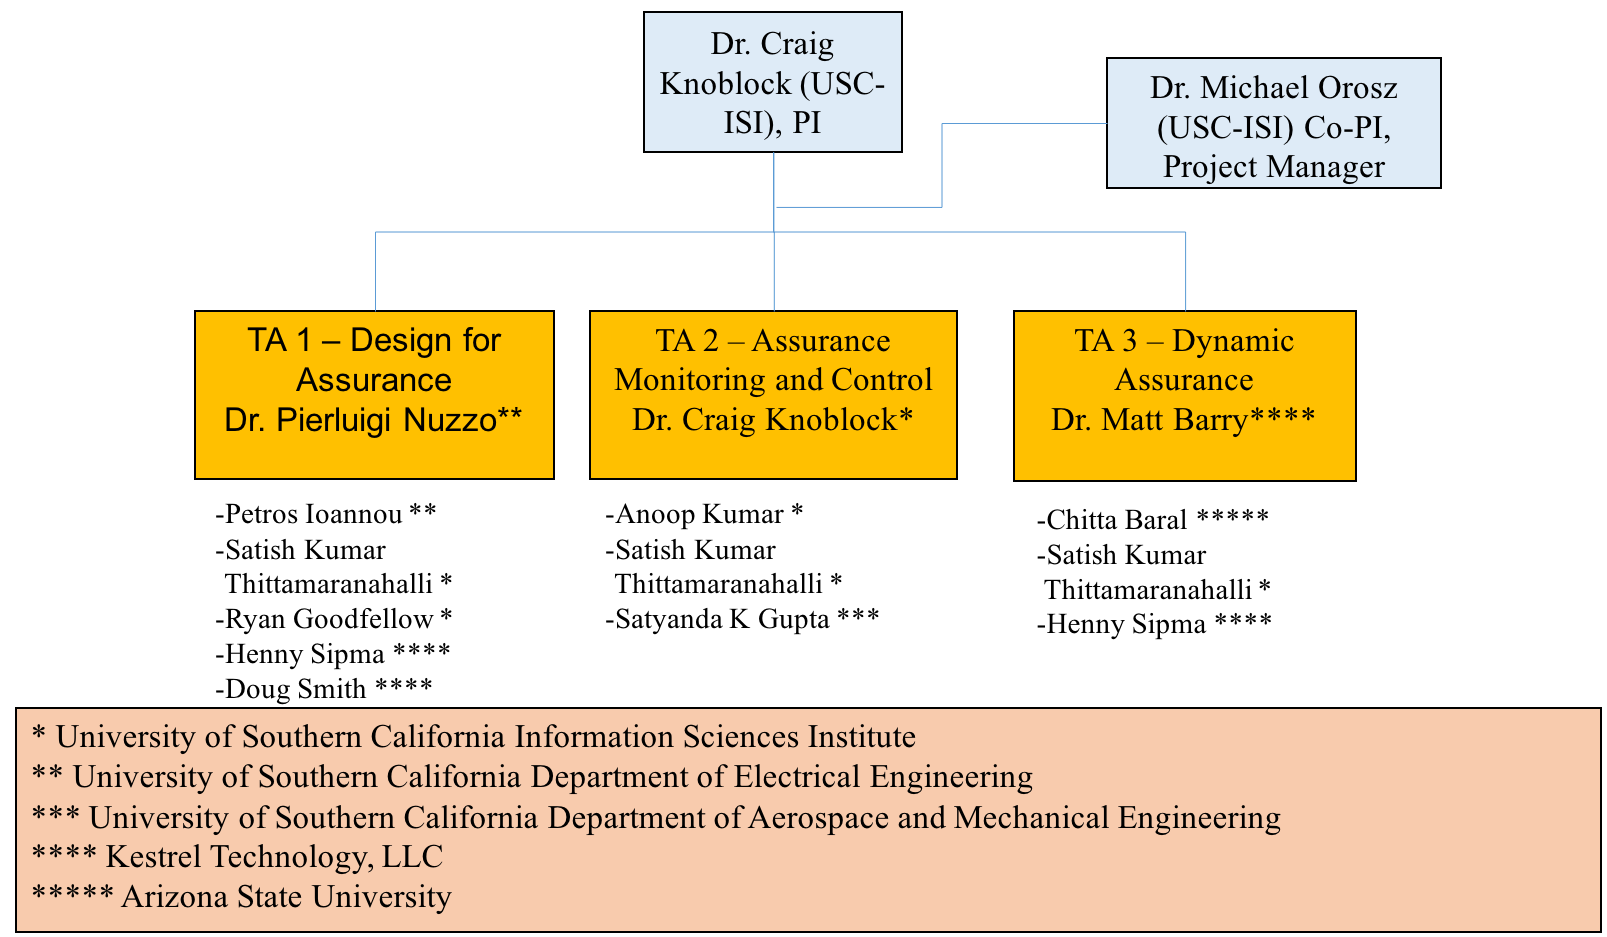
\includegraphics[width=6.0in]{./org-chart2.png}
\caption{\small Organization Chart}
\label{fig:org_chart}
\end{figure}

Coordination: To maximize collaboration and reduce risk to project failure from lack of communication and technical exchange, we plan to employ a wide variety of working styles and communication/coordination so that all can contribute.  At the core of our project will be regularly scheduled meetings bridging the diversely distributed team (Table~\ref{fig:Collaboration_Table}).  These meetings will address project status, identify challenges, implement risk mitigation strategies and participate in technology exchanges and system integration efforts (when appropriate)

\begin{table}[ht]
\caption{\small Project Meetings and Events}
  \centering
  {\footnotesize
\begin{tabular}{|m{3.15in}|m{3in}|} 
\hline
\textbf{Meeting} & \textbf{Frequency} 
\\\hline
Conference calls among investigators (discuss project status, address concerns and project risks) & Weekly
\\
\hline
Technical exchange and coordination meetings using Bluejeans or another videoconference technology & At least twice a month and more frequently as needed
  \\ 
\hline
Face-to-Face meetings (prior to P/I and demonstration meetings) & Every 3 to 6 months and more frequently (especially at the beginning of the project) as needed
 \\\cline{1-2}

\hline
\end{tabular}
}
\label{fig:Collaboration_Table}
\end{table}

\begin{table}[tbhp]
\caption{\small Key Project Team Member Responsibilities}
  \centering
  {\footnotesize
\begin{tabular}{| m{.75in} | m{3.9in}| m{1.5in}|} 
\hline
\textbf{Key Member} & \textbf{Responsibilities} & \textbf{Tasks} 
\\\hline
Dr.\ Craig Knoblock  & Principal Investigator responsible for project, leads TA 2 – Assurance Monitoring and Control.  Will lead the overall project and lead the TA2 team.  Served as the PI on many DARPA projects and has sucessfully led many large teams.    Effort on project:  25\% &
1.1.6, 1.2.2 1.2.3, 1.2.4, 1.3.4, 1.4.1, 
2.1.6, 2.2.2 2.2.3, 2.2.4, 2.3.4, 2.4.1, 
3.1.6, 3.2.2, 3.2.3, 3.2.4, 3.3.4, 3.4.1
\\
\hline
Dr.\ Michael Orosz & Co-Principal Investigator responsible managing the day-to-day operations of the project, assist technical teams as needed, coordinate with TA4 teams.    Has led many large complex multi-disciplined/multi-organizational projects in academic and industry environments.  Effort on project: 50\%
& 1.1.6, 2.1.6, 3.1.6, 1.4.1, 2.4.1, 3.4.1
  \\ 
\hline
Dr.\ Pierluigi Nuzzo 
& 
Co-Principal Investigator.  Leads the TA 1 - Design for Assurance team and conducts research on the formal methods for the design of the TA1 system.  Research experience on methodologies and tools for the design of cyber-physical systems; contracts, interfaces, and compositional methods for embedded system design; the application of automated formal methods and optimization theory to problems in embedded and cyber-physical systems.  Effort on project: 2 months/year (16.6\%)
& 
1.1.1, 2.1.1, 3.1.1 \\
\hline
Dr.\ Matthew Barry
& 
Key personnel.  Leads the TA 3 – Dynamic Assurance.   He will conduct the research on the dynamic assurance case language editors and parsers, the run-time system, and system integrations. Effort on project:  66\%
& 
1.3.2, 2.3.2, 3.3.2\\
\hline
Dr.\ Chitta Baral
& 
Key personnel responsible for learning assurance rules, supporting assurance rules with uncertainty and improving solver speed.  Expertise on ASP solvers, which will be used to reason about the assurance cases. Effort on project: 20\%
& 
1.3.1, 2.3.1, 3.3.1 \\
\hline
Dr.\ Doug Smith 
& 
Key personnel will support formal methods aspects of TA1, and lead the effort on abstract refinement. Expertise in field of automated correct-by-construction program generation.    Effort on project: 40\%
& 
1.1.5, 2.1.5, 3.1.5 \\
\hline
Dr.\ Henny Sipma
& 
Key personnel who will support the program verification tasks under TA1.  Will lead the effort on program verification.   Effort on project:  45\%
& 
1.1.5, 2.1.5, 3.1.5, 1.3.2, 2.3.2, 3.3.2 \\
\hline
Dr.\ Petros Ioannou
& 
Key personnel responsible providing and extending the assurance test bed, which will be available at the start of the project for autonomous vehicles.   Effort on project: 1 month/year (8.3\%)
& 
1.1.2, 2.1.2 (optional), 3.1.2 (optional)
\\
\hline
Dr.\ Satyandra Kumar Gupta
& 
Key Personnel providing autonomous command and control expertise to the TA-2 team.   Will lead the research on safety aware learning on TA2.   Past research on physics-aware decision making to facilitate automation.  Effort on project: 1 month/year (8.3\%)
& 
1.2.1, 2.2.1, 3.2.1 \\
\hline
Dr.\ Anoop Kumar 
& 
Key personnel providing support to the TA 2 project team.  Will lead the research on monitoring \& control and detecting distribution shifts.  Effort on project: 50\%
& 
1.2.1, 1.2.2, 1.2.3, 1.2.4, 2.2.1, 2.2.2, 2.2.3, 2.2.4, 3.2.1, 3.2.2, 3.2.3, 3.2.4\\
\hline
Dr.\ Satish Thittamaranahalli
& 
Key personnel developing scalable algorithms for TA1, TA2, and TA3 project teams.  Has extensive experience on scalable algorithm design, machine learning, and constraint reasoning.  Effort on project: 50\%
& 
1.2.1, 1.2.2, 1.2.3, 1.2.4, 2.2.1, 2.2.2, 2.2.3, 2.2.4, 3.2.1, 3.2.2, 3.2.3, 3.2.4, 1.1.4, 2.1.4, 3.1.4 \\
\hline
Dr.\ Ryan Goodfellow
& 
Key personnel providing support to the TA-1 project. Will lead the research on simulation-based testing.  Has extensive experience on simulation-based testing.  Effort on project:  30\%
& 
1.1.3, 2.1.3, 3.1.3 \\

\cline{1-2}

\hline
\end{tabular}
}
\label{fig:Table_Mgmt}
\end{table}



\newpage
\section{Personnel, Qualifications and Commitment}

{\bf Dr.\ Craig Knoblock}, the PI on this effort, is a Research Professor of both Computer Science and Spatial Sciences at the University of Southern California (USC) and Director of the Intelligent Systems Division at the USC Information Sciences Institute.   He received his Ph.D. from Carnegie Mellon University in computer science. 
%His research focuses on techniques for describing, acquiring, and exploiting the semantics of data.  
In previous projects he has worked on developing  scalable approaches to execution monitoring, accurate detection of sensor failures, and   automatic modeling and reconstruction of sensors.  He has published more than 300 journal articles, book chapters, and conference papers on these topics.  Dr. Knoblock is a Fellow of the Association for the Advancement of Artificial Intelligence (AAAI), a Distinguished Scientist of the Association of Computing Machinery (ACM), a Senior Member of IEEE, past President and Trustee of the International Joint Conference on Artificial Intelligence.
%and winner of the 2014 Robert S. Engelmore Award.  

{\bf Dr.\ Michael Orosz}, a Co-PI on this effort, is a Research Associate Professor of Civil and Environmental Engineering at the University of Southern California (USC) and Research Director of the Decision Systems Group at the USC Information Sciences Institute.  Dr. Orosz has over 30 years’ experience in commercial and government software development, basic and applied research, project management, academic research and has developed and deployed several commercially successful products.  His research interests are in machine learning and decision analytics as applied to intelligence analysis and autonomous command and control such as smart building controls.    Dr. Orosz has extensive experience in managing large complex multi-disciplined/multi-teamed research projects. %funded by DARPA, DHS, DoD, DoE, Industry, NASA, NRO, NSA and ONR.   
He received his Ph.D. in computer science from the University of California, Los Angeles.

{\bf Dr.\ Pierluigi Nuzzo}, a Co-PI on this project, is an Assistant Professor in the Department of Electrical Engineering at the University of Southern California. He received the Ph.D. in Electrical Engineering and Computer Sciences from the University of California at Berkeley. 
%in 2015, and the Laurea degree (MS) in electrical engineering (summa cum laude) from the University of Pisa, Italy, and the Sant'Anna School of Advanced Studies, Pisa, Italy.
%
%He has four years of research experience in analog and mixed signal circuit design as a researcher at IMEC, Leuven, Belgium, and over 10 years experience in design methodologies and tools for mixed-signal integrated circuits and cyber-physical systems, as a researcher at the University of Pisa, IMEC, UC Berkeley, and USC. 
His research interests
include: methodologies and tools for cyber-physical system and mixed-signal
system design; contracts, interfaces and compositional methods for embedded
system design; the application of formal methods and optimization theory to problems in embedded and cyber-physical systems and electronic design automation. 
%
Prof. Nuzzo received %First Place in the operational category and Best Overall
%Submission in the 2006 DAC/ISSCC Design Competition, 
a Marie Curie Fellowship
from the European Union in 2006, 
the University of California at Berkeley EECS
departmental fellowship in 2008, 
%the University of California at Berkeley Outstanding Graduate Student Instructor Award in 2013, 
the IBM Ph.D.
Fellowship in 2012 and 2014, 
%the Best Paper Award from the International Conference on Cyber-Physical Systems (ICCPS) in 2016, 
and the David J.~Sakrison Memorial Prize in 2016 for his doctoral research. 
%He is an author of 1 patent and over 60 publications.

{\bf Dr.\ Satyandra K. Gupta} is Smith International Professor in the Department of Aerospace and Mechanical Engineering at the University of Southern California. %Prior to joining the University of Southern California, he was a Professor in the Department of Mechanical Engineering and the Institute for Systems Research at the University of Maryland. He was the founding director of the Maryland Robotics Center and the Advanced Manufacturing Laboratory at the University of Maryland. 
He served as a program director for the National Robotics Initiative at the National Science Foundation from September 2012 to September 2014.  Dr. Gupta's interest is in the area of physics-aware decision making to facilitate automation. He has published more than 300 technical articles. He is a fellow of the American Society of Mechanical Engineers (ASME) and editor of ASME Journal of Computing and Information Science in Engineering. Dr. Gupta has received the Young Investigator Award from the Office of Naval Research in 2000, CAREER Award from the National Science Foundation in 2001, Presidential Early Career Award for Scientists and Engineers (PECASE) in 2001, Invention of the Year Award at the University of Maryland in 2007, Kos Ishii-Toshiba Award from ASME in 2011, and Excellence in Research Award from ASME in 2013.%, and Distinguished Alumnus Award from Indian Institute of Technology, Roorkee in 2014. %He has also received seven best paper awards at conferences.

{\bf Ryan Goodfellow} is a computer scientist at ISI working in combined cyber physical simulation and emulation platform development. His formal background is in simulation algorithms and modeling techniques using differential-algebraic equations (DAE). He has applied this knowledge in the CPS space by integrating DAE modeling languages and simulation engines with network testbeds to create comprehensive scientific experimentation platforms for cyber-physical systems. These experimentation platforms have been used in the power grid research space. %Ryan is a lead developer on the Deter network testbed, with a strong background in networked and distributed systems engineering. %He is also a combat veteran, serving as a non-commissioned officer and SIGINT team lead for a multi-functional intelligence team in Afghanistan.

{\bf Dr.\ Petros Ioannou} is a Professor in the Department of Electrical Engineering, Director of the Center for Advanced Transportation Technologies and Associate Director for Research for the DOT supported University Transportation Center at USC. He received his MS and PhD from the University of Illinois at Urbana Champaign in Mechanical and Electrical Engineering, respectively. His research interests are in robust adaptive control, vehicle dynamics and control, human factors and safety, automated vehicles, nonlinear systems and Intelligent transportation Systems.  He received the 2016 IEEE Transportation Technologies field award and the 2016 IEEE Control system society Transition to Practice Award. He is a Fellow of IEEE, IFAC and IET and author/coauthor of 8 books and over 400 papers.

{\bf Dr.\ Matthew Barry} will serve as lead for the TA3 tasks. %He will implement the dynamic assurance case language editors and parsers, the run-time system, and system integrations.  He will implement the assurance case arguments and the API for updating argument structure and content.  
Dr. Barry currently is CEO at Kestrel Technology LLC, and previously spent 20 years in NASA space mission operations at the Jet Propulsion Lab and Johnson Space Center.  At NASA Headquarters he led the introduction of dependability case requirements and plans for flight computing systems in upcoming manned space exploration missions, as well as the development of Agency-level software-related safety-critical control system requirements.  He recently served as a Principal Investigator on DHS/Cyber S\&T STAMP (Static Tool Analysis Modernization Program), DARPA CSFV (Crowd Sourced Formal Verification), three NASA Aeronautics R\&D projects, and the AFRL-sponsored Static Analysis of Numerical Algorithms project.  Dr. Barry earned BSME, MS, and PhD degrees in mechanical engineering, and an MBA degree, from Rice University.  

{\bf Dr.\ Henny Sipma} will support the program verification tasks under TA1.  %She is the key person behind the company's {\em KT Advance\/} and {\em KT Transferal\/} static analysis products, and the designer and programmer of the company's core {\em CodeHawk\/} abstract interpretation engine. 
Dr. Sipma currently is the CTO at Kestrel Technology LLC.  She has spent the past 10 years with Kestrel Technology as a static analysis expert; previously developed and taught static analysis techniques as senior research associate at Stanford University for eight years; and developed industrial process controls as an senior systems analyst at Shell.  She has been Principal Investigator or company lead on several recent R\&D projects for Federal agencies, including two projects under the IARPA STONESOUP (Securely Taking On New Executable Software of Uncertain Provenance) program; the DHS Cyber S\&T Gold Standard project; and the DARPA-sponsored STAC (Space-Time Analysis for Cybersecurity) and MUSE (Mining and Understanding Software Enclaves) programs.  Dr. Sipma earned 
%a BS degree in chemistry and an MS degree in chemical engineering at the University of Groningen in The Netherlands, and 
MS and PhD degrees in computer science from Stanford University.  

{\bf Dr.\ Douglas R.\ Smith} will support formal methods aspects of TA1, including the enforcement of safety properties and the generation of monitors.  He is President of Kestrel Technology LLC and Principal Scientist at Kestrel Institute.  He is a Fellow of the American Association of Artificial Intelligence (AAAI) and an ASE Fellow (Automated Software Engineering).  From 1986 to 2000, he taught an advanced graduate course on correct-by-construction software development at Stanford.  
%Dr. Smith has led the development of a series of software synthesis systems, including KIDS (Kestrel Interactive Development System), Specware, Designware, and Planware. 
%Applications domains have included a variety of complex high-performance planners and schedulers for the US Air Force.  He leads current projects on the generation of air mission plans and cyberoperations.  
Other recent projects focused on automated policy enforcement \cite{SmithD0703,SmithD08}, synthesis of secure network protocol codes, and the synthesis of high-performance constraint-solvers\cite{SmithD08c,SmithD13}.  Dr. Smith has over 30 years experience in the field of automated correct-by-construction program generation and has published over 100 papers. He has one patent.  He received the Ph.D. in Computer Science from Duke University% in 1979.  

{\bf Dr. Chitta Baral} is a Professor in the Department of Computer Science and Engineering at Arizona State University. He will support the TA3 efforts on Learning assurance rules, supporting assurance rules with uncertainty and improving solver speed. Dr. Baral has expertise in various aspects of autonomy and Artificial Intelligence. 
He wrote the first book on answer set programming (published by Cambridge University Press) the formal language behind our assurance rules. Some of his other works relevant to this proposal are: goal specification for autonomous systems, automatic construction of control rules for autonomous systems that satisfy given goals, combining machine learning with reasoning in various contexts, including image understanding. %He is the President of KR Inc. He is an associate editor of AIJ and has been an associate editor of JAIR.

{\bf Dr.\ Satish Kumar Thittamaranahalli (T. K. Satish Kumar)} leads the Collaboratory for Algorithmic Techniques and Artificial Intelligence (CATAI) at USC's Information Sciences Institute. He has published over 60 papers on numerous topics in Artificial Intelligence spanning such diverse areas as Constraint Reasoning, Planning and Scheduling, Probabilistic Reasoning, Robotics, Combinatorial Optimization, Approximation and Randomization, Heuristic Search, Model-Based Reasoning, Knowledge Representation and Spatio-Temporal Reasoning. %He %has served on the Program Committees of many international conferences in Artificial Intelligence
He and is a winner of the 2016 Best Robotics Paper Award and the 2005 Best Student Paper Award from the International Conference on Automated Planning and Scheduling. 
Dr. Kumar received his PhD in Computer Science from Stanford University. %In the past, he has also been a Visiting Student at the NASA Ames Research Center, a Postdoctoral Research Scholar at the University of California, Berkeley, a Research Scientist at the Institute for Human and Machine Cognition, a Visiting Assistant Professor at the University of West Florida, and a Senior Research and Development Scientist at Mission Critical Technologies.

\textbf{Dr.\ Anoop Kumar} is a senior computer scientist at USC ISI and has broad expertise in machine learning, statistical modeling, and software engineering.  Dr.\ Kumar is the technical lead on the DARPA RSPACE program and has played a vital role in developing a system that fuses air operations data from multiple sources, maintains world state, and issues warnings. Previously, he led the research and development of the BBN’s election forecasting system for the IARPA OSI program. %Dr.\ Kumar played a significant role in the DARPA DEFT program by developing a model to support integration of output from multiple NLP algorithms. He has contributed at the development to management levels on government research contracts and commercial projects. 
Dr.\ Kumar helped design and develop BBN's commercially available, hosted speech and medical transcription services offering. 

\begin{table}[!tbh]
\begin{footnotesize}
\vspace{-0.1in}

\begin{tabular}{lll}
\begin{tabular}[t]{|l|@{}c@{}|@{}c@{}|@{}c@{}|@{}c@{}|} \hline
Project & Status & \multicolumn{3}{ c| }{Hours} \\ \cline{3-5}
& & P1 & P2 & P3 \\ \hline



\multicolumn{5}{ |c| }{ \textbf{Craig Knoblock} } \\ \cline{1-5}
Safeguard & Pro & 770 & 641 & 641 \\ \cline{1-5}
ELICIT & Cur & 308 & 256 & 120 \\ \cline{1-5}
WTNIC & Cur & 11 & 0 & 0 \\ \cline{1-5}
EFFECT & Cur & 641 & 107 & 0 \\ \cline{1-5}
LinkedMaps & Cur & 203 & 25 & 0 \\ \cline{1-5}
PRINCESS & Cur & 608 & 96 & 0 \\ \cline{1-5}
SCHARP & Cur & 481 & 54 & 0 \\ \cline{1-5}
MINT & Pen & 650 & 534 & 285 \\ \cline{1-5}

\multicolumn{5}{ |c| }{ \textbf{Michael Orosz} } \\ \cline{1-5}
Safeguard & Pro & 1560 & 1300 & 1300  \\ \cline{1-5}
SMC/SY & Cur & 1803 & 0 & 0  \\ \cline{1-5}

\multicolumn{5}{ |c| }{ \textbf{Matthew Barry} } \\ \cline{1-5}
Safeguard & Pro & 2078 & 1690 & 1554 \\ \cline{1-5}
Starlite & Cur & 1840 & 1692 & 0 \\ \cline{1-5}



\multicolumn{5}{ |c| }{ \textbf{Anoop Kumar} } \\ \cline{1-5}
Safeguard & Pro & 1560 & 1300 & 1300 \\ \cline{1-5}

\end{tabular}
&
\begin{tabular}[t]{|l|@{}c@{}|@{}c@{}|@{}c@{}|@{}c@{}|} \hline
Project & Status & \multicolumn{3}{ c| }{Hours} \\ \cline{3-5}
& & P1 & P2 & P3 \\ \hline

\multicolumn{5}{ |c| }{ \textbf{Pierluigi Nuzzo} } \\ \cline{1-5}
Safeguard & Pro & 520 & 433 & 433  \\ \cline{1-5}
Mirage & Cur & 433 & 0 & 0  \\ \cline{1-5}

\multicolumn{5}{ |c| }{ \textbf{Satyandra Gupta} } \\ \cline{1-5}
Safeguard & Pro & 260 & 217 & 217 \\ \cline{1-5}
Human   & Cur & 22 & 0 & 0 \\ \cline{1-5}
Vehicles & Cur & 36 & 0 & 0 \\ \cline{1-5}
Robot & Cur & 116 & 0 & 0 \\ \cline{1-5}
Assembly & Cur & 33 & 0 & 0 \\ \cline{1-5}
Solar & Cur & 4 & 0 & 0 \\ \cline{1-5}

\multicolumn{5}{ |c| }{ \textbf{Petros Ioannou} } \\ \cline{1-5}
Safeguard & Pro & 260 & 217 & 217 \\ \cline{1-5}
CPS & Cur & 130 & 0 & 0 \\ \cline{1-5}

\multicolumn{5}{ |c| }{ \textbf{Ryan Goodfellow} } \\ \cline{1-5}
Safeguard & Pro & 936 & 780 & 780 \\ \cline{1-5}
STEAM & Cur & 416 & 0 & 0 \\ \cline{1-5}


\end{tabular}
&
\begin{tabular}[t]{|l|@{}c@{}|@{}c@{}|@{}c@{}|@{}c@{}|} \hline
Project & Status & \multicolumn{3}{ c| }{Hours} \\ \cline{3-5}
& & P1 & P2 & P3 \\ \hline

\multicolumn{5}{ |c| }{ \textbf{Chitta Baral} } \\ \cline{1-5}
Safeguard & Pro & 659 & 485 & 485 \\ \cline{1-5}
PostdocBP & Cur & 176 & 0 & 0 \\ \cline{1-5}
Languages & Pen & 528 & 264 & 264 \\ \cline{1-5}
CAREER & Pen & 88 & 44 & 44 \\ \cline{1-5}
CHS & Pen & 510 & 255 & 0 \\ \cline{1-5}

\multicolumn{5}{ |c| }{ \textbf{Doug Smith} } \\ \cline{1-5}
Safeguard & Pro & 1222 & 984 & 840 \\ \cline{1-5}
RSPACE & Cur & 342 & 0 & 0 \\ 
\cline{1-5}
PLANX & Cur & 154 & 0 & 0 \\ 
\cline{1-5}
HACCS & Pen & 923 & 769 & 769 \\ 
\cline{1-5}

\multicolumn{5}{ |c| }{ \textbf{Henny Sipma} } \\ \cline{1-5}
Safeguard & Pro & 1372 & 962 & 840 \\ \cline{1-5}
STAC & Cur & 797 & 0 & 0 \\ \cline{1-5}

\multicolumn{5}{ |c| }{ \textbf{Satish Thittamaranahalli} } \\ \cline{1-5}
Safeguard & Pro & 1560 & 1300 & 1300 \\ \cline{1-5}
MapF & Cur & 103 & 103 & 0 \\ \cline{1-5}

\end{tabular}
\end{tabular}

\end{footnotesize}
\caption{Individual commitments of key personnel}
\label{tab:Commitments}
\vspace{-0.2in}
\end{table}

\clearpage
\newpage
\section{Capabilities}


%\subsection{University of Southern California}
USC has strengths in number of areas that are closely related to the proposed work:
\begin{itemize}[itemsep=0pt,leftmargin=*]
\item Dr.\ Nuzzo 
%has over 10-year research experience in embedded system design, from mixed-signal chip design (analog-to-digital converters, frequency synthesizers, software-defined radio), to methodologies and tools for mixed-signal integrated circuits and Cyber-Physical Systems (CPSs), and the application of formal methods and optimization theory to problems in embedded and cyber-physical systems and electronic design automation.  
%His doctoral work 
has done extensive research on contracts and compositional methods for heterogeneous system design and design space exploration, with application to aircraft electric power systems and environmental control systems. His work has helped transition rigorous system design foundations, innovative design methodologies, and new systems engineering paradigms to industry (IBM, United Technologies). 
\item Dr.\ Satyandra K. Gupta has worked on autonomous surface vehicles, autonomous ground vehicles for operation on rugged terrains, and autonomous flapping wing aerial vehicles.   His group has developed a hierarchal decision making approach for realizing autonomous systems. 
%This approach combines task planning and assignment, deliberative trajectory planning, reactive collision avoidance behaviors, and trajectory tracking control layers. 
His group has also developed new methods for learning reactive behaviors in adversarial environments and COLREGS compliant trajectory planning. \item Dr.\ Knoblock has developed methods that learn the relationships between sensors to both identify failures and changes in sensor and reconstruct those sensors, providing estimates of the accuracy of the reconstructed sensors.  
\item Ryan Goodfellow has extensive experience in simulation based testing through high-fidelity CPS testbed environment development and operation, using the Deter network testbed as the core which has supported several large scale government projects from a variety of agencies and thousands of users. %we have developed sophisticated CPS experiments under programs such as NFS RIPS, NIST SmartCities and the DHS Cybersecurity showcase.
\item Dr.\ Ioannou %helped  design and implement adaptive cruise control systems in collaboration with Ford Motor Company, which was commercialized four years before any other company. He 
worked on several DOT funded projects on automated vehicles and intelligent highway systems where he demonstrated his vehicle control designs for safety and performance on actual automated vehicles in test trucks and I-15 highway.
\item Drs.\ Knoblock, Kumar, and Thittamaranahalli have developed highly scalable approaches for monitoring message traffic to identify potential problems and issue warnings and alerts. 
\item Dr. Thittamaranahalli has developed state-of-the-art methods for efficiently solving large-scale search and optimization problems. %These techniques will be applicable in TA2 for safety-aware learning and planning, in TA2 for assurance monitoring and control, and in TA3 for dynamic assessment of assurance cases.

\end{itemize}
%\subsection{Kestrel Technology LLC}

Kestrel Technology's strength is in program analysis, specifically static analysis of both source and binary targets.  The company performs applied R\&D and product development for a variety of static analysis applications  pivoting primarily on the abstract interpretation technique.  The company recently initiated development of program analysis applications using logical equivalence techniques. As a provider of verification evidence in the form of mathematical proofs, the company also has expertise in the design and development of assurance case arguments for high-integrity systems using such evidence. %The company is engaged in a partnership with Wind River Systems to develop program analysis tools for its embedded system developers.  Many of Wind River's customers must develop their products under safety and certification standards, including those using safety cases.  

   

%\subsection{Arizona State University}
Chitta Baral at Arizona State University has developed various software to learn assurance rules and various ASP solvers, which he has made available as open-source.

Most of the software carried forward for implementation or derivation is open source.  The single exception is Kestrel Technology's {\it KT Advance\/} static analysis tool (TA1), in particular the abstract interpretation engine therein, which is company proprietary and is US EAR export-controlled.   
%Owing to mixed funding for the development of that technology 
We will continue to provide the Federal government a restricted use license for that particular item.

There are no specialized facilities, data, or GFE required for this effort. 

\include{sow}
\include{milestones}

% \section{Level of Effort by Task \textcolor{red}{[Mike/Lisa - 1 pages]}}

% \textcolor{blue}{
% \begin{itemize}
% \item Will be a separate spreadsheet
% \item
% \end{itemize}
% }

\include{appendix_a}

%\section{Appendix B \textcolor{red}{[No Page Count]}}

\section{References}
\bibliographystyle{acm} 
\bibliography{TA3/ta3,TA2/ta2,TA1/ta1}
\end{document}
%%\documentclass[a4paper]{article}
%\documentclass[12pt]{article}
\documentclass[12pt]{dod-blank}

%% Language and font encodings
\usepackage[english]{babel}
\usepackage[utf8x]{inputenc}
\usepackage[T1]{fontenc}

%% Sets page size and margins
%%\usepackage[a4paper,top=3cm,bottom=2cm,left=3cm,right=3cm,marginparwidth=1.75cm]{geometry}
%\usepackage[top=1in, bottom=1in, left=1in, right=1in]{geometry}



%% Useful packages
\usepackage{amsmath}
\usepackage{graphicx}
  \graphicspath{{.}{./image/}}
  \DeclareGraphicsExtensions{.png,.jpg} 
\usepackage[colorinlistoftodos]{todonotes}
\usepackage[colorlinks=true, allcolors=blue]{hyperref}
\usepackage{tabularx}
\usepackage{multirow}
\usepackage{tabulary}
\usepackage{float}
\usepackage{wrapfig}
\usepackage[export]{adjustbox}
\usepackage{comment}
\usepackage{tabularx}
\usepackage{multirow}
\usepackage{tabulary}
\usepackage{enumitem}

\usepackage{listings}
\usepackage{color}
\usepackage{array}
\usepackage{subcaption}
\usepackage{xcolor}




\renewcommand{\textfraction}{0}
\renewcommand{\topfraction}{1.0}
\renewcommand{\bottomfraction}{1.0}

\usepackage{longtable}
%% macros
\newif\iffinal
\finaltrue
\iffinal
  
    \newcommand\baareq[1]{}
    \newcommand\baades[1]{}
 
 
\else
    \definecolor{darkgreen}{rgb}{0,0.4,0}
    \definecolor{darkcyan}{rgb}{0,0.4,0.4}
    \definecolor{darkblue}{rgb}{0,0,0.5}
    
    \newcommand\baareq[1]{{\color{darkcyan}[\textbf{Requirement:} #1]}}
    \newcommand\baades[1]{{\color{darkcyan}[\textbf{Description:} #1]}}
 
\fi




\def\naive{na\"{\i}ve}



\lstset{ 
  backgroundcolor=\color{white},   % choose the background color; you must add \usepackage{color} or \usepackage{xcolor}
  basicstyle=\footnotesize\ttfamily,            % the size of the fonts that are used for the code
  breakatwhitespace=false,         % sets if automatic breaks should only happen at whitespace
  breaklines=true,                 % sets automatic line breaking
  captionpos=b,                    % sets the caption-position to bottom
  commentstyle=\color{mygreen},    % comment style
  % deletekeywords={...},            % if you want to delete keywords from the given language
  escapeinside={\%*}{*)},          % if you want to add LaTeX within your code
  extendedchars=true,              % lets you use non-ASCII characters; for 8-bits encodings only, does not work with UTF-8
  frame=single,	                   % adds a frame around the code
  keepspaces=false,                 % keeps spaces in text, useful for keeping indentation of code (possibly needs columns=flexible)
  keywordstyle=\color{blue}\bfseries\underbar,       % keyword style
  language=Prolog,                 % the language of the code
  % morekeywords={if,and},        % if you want to add more keywords to the set
  numbers=none,                    % where to put the line-numbers; possible values are (none, left, right)
  numbersep=5pt,                   % how far the line-numbers are from the code
  numberstyle=\tiny\color{mygray}, % the style that is used for the line-numbers
  rulecolor=\color{black},         % if not set, the frame-color may be changed on line-breaks within not-black text
  showspaces=false,                % show spaces everywhere adding particular underscores; it overrides 'showstringspaces'
  showstringspaces=false,          % underline spaces within strings only
  showtabs=false,                  % show tabs within strings adding particular underscores
  stepnumber=2,                    % the step between two line-numbers. If it's 1, each line will be numbered
  stringstyle=\color{mymauve},     % string literal style
  tabsize=2,	                   % sets default tabsize to 2 spaces
  title=\lstname                   % show the filename of files included with \lstinputlisting; also try caption instead of title
}

% apply trick for additional keywords for our AC DSL
\lstset{
	emph={for, if, and, or},
    emphstyle={\color{blue}\bfseries\underbar}
}




\title{DARPA Assured Autonomy}
\author{Technical Volume- \textcolor{red}{Thirty-Eight (38) pages max}}

\begin{document}
\pagenumbering{roman}
\include{cover}

\newpage
\section{Table of Contents}
\tableofcontents

\newpage
\pagenumbering{arabic}
\section{Executive Summary}
As we rapidly move into a world where machine learning plays a central role in realizing autonomous systems, it is becoming increasingly important to develop techniques that assure that these systems will operate safely and perform as expected. Current approaches are limited to providing assurance for systems with limited or no  learning capabilities. In this context, DARPA's Assured Autonomy BAA seeks to \emph{develop rigorous design and analysis technologies for continual assurance of learning-enabled autonomous systems}. USC in collaboration with Kestrel Technology and ASU is pleased to submit a comprehensive TA1, TA2, and TA3 proposal entitled \emph{``Assured Autonomy for Learning Enabled Vehicles (Safeguard).''} We plan to provide an end-to-end solution to support autonomous systems with learning-enabled components, ranging from design technologies for assurance, to assurance monitoring and control techniques, to representation and online evaluation of assurance cases. We have assembled a strong team of experts that cover the range of technologies that are required to create such an end-to-end system. If successful, the project will provide the technologies for building the next-generation of learning-enabled autonomous systems.  The entire project will take four years and cost \textcolor{red}{\$??}, with an initial version completed at the end of Phase I and successive versions with additional capabilities and improved scalability at the end of Phase II and Phase III.  

In the remainder of this section, we first introduce an  unmanned surface vehicle scenario that will be used throughout the proposal to describe the approach.  Next, we describe our approach to design, monitoring, and dynamic assurance. Finally, we introduce the team involved in the project. 

\textbf{Motivating Scenario.} Consider an autonomous unmanned surface vehicle (USV) guarding a valuable asset in the ocean when an unknown vehicle  approaches the security perimeter, under challenging weather conditions. In this scenario, the USV is required to approach the intruding vehicle, issue a warning signal, and escort it to a safe distance from the controlled area. However, as the USV has no a priori knowledge of its external environment behaviors (e.g., water depth, waves, wind, current, visibility), pre-computing a feasible trajectory, let alone optimal, becomes a non-trivial problem. For trajectory planning, the USV must continuously perform the following tasks:
\begin{itemize}[itemsep=0pt,leftmargin=*]
 \item Sense the current state of the surrounding environment (e.g., water depth, waves, wind, current, visibility) and estimate its own maneuverability constraints (e.g., braking distance, available acceleration, maximum velocity, turning radius, turning rate, safety distance) based on the state of the environment;      
\item Sense the static obstacles in the sensor range and generate a traversability map;
\item Sense the moving obstacles and classify them;   
\item Predict future trajectories of moving obstacles; 
\item Determine if any of the COLREGS \cite{commandant1999international} rules will be in effect with respect to one or more of the nearby vessels and identify the vessels with the right of way.    
\end{itemize}
The above information will be used by the trajectory planner to compute an initial trajectory, which will be continuously refined as the USV gathers additional information.
% It is not possible for the USV to be tested in every possible environment. 
The USV will use learning enabled components to take  decisions as it encounters new situations, such as  
\begin{itemize}[itemsep=0pt,leftmargin=*]
\item Classifiers to identify moving obstacles based on physical appearance and motion signatures,
\item Algorithms to estimate the sensor capabilities in adverse weather conditions,   
\item Algorithms to accurately estimate uncertainty in the environment, 
\item Classifiers to generate traversability maps,
\item Prediction of external vessel behaviors based on motion histories, 
\item Reinforcement learning  to ensure COLREGS compliance of maneuvers,  
\item Algorithms to learning pursuit behaviors.  
\end{itemize}
Learning enabled components will interact with each other in complex ways, where a misclassification error in one component may eventually compromise the entire mission.   
% We will need to make sure that each learning enabled components has a run-time monitor that will ensure that the assumptions made by the learning-enabled component remain valid and prevent erroneous learning. 
% For example, if the vehicle is exhibiting significant error in trajectory tracking, then simply downgrading the trajectory tracking error value may not be a good option.  The failure of prediction of trajectory tracking error might be due to the presence of a significant wake caused by a nearby vessel. The presence of the nearby vessel can be used to explain the degradation in trajectory tracking performance. As the vessel moves away, we can expect the trajectory tracking performance to return to the predicted level.  
While exhaustive validation of learning-enabled cyber-physical systems (LE-CPSs) is a prohibitive task~\cite{Kalra16},
their complexity, heterogeneity, and highly dynamic nature
make it challenging to even leverage existing model-based development techniques to effectively assess system correctness 
% dependability, 
at design time or enforce it at runtime.

\textbf{Design for Assurance.} Safeguard uses a platform-based design approach~\cite{Nuzzo15b} to organize the design process for a LE-CPS and to build assurance cases. Composite models are developed at several levels of abstraction,
from top-level system requirements and safety constraints down to the
implementation level.  Intermediate levels add detail to the levels
above.  The different levels are connected by refinement mappings that
allow properties established at one level to be preserved at the next
level (see Figures~\ref{fig:methodology} and~\ref{fig:assurance}).

Contracts are used to formally specify components and composite models
in terms of (1) Assumptions -- the assumed behaviors of the
environment and the behaviors of other components, and (2) Guarantees
-- the behavior properties that a model guarantees if it operates in a
context that satisfies its assumptions.  A calculus of contracts
allows horizontal composition of contracts to generate contracts for
composite models.  Vertical contracts are used to specify the mapping
or refinement relation between models at different levels of
abstraction.  The system design process starts with a high-level
contract that expresses overall system assumptions and requirements.
Subsequent levels express models with increasing detail until the
lowest level expresses the system in terms of hardware components and
their software controllers.

The assurance case for a CPS arises from the horizontal and vertical
structure of the design in several ways.  The components used within a
particular level are either (1) synthesized using
correct-by-construction design tools together with proofs, (2) derived
statically or dynamically using safety-aware machine-learning
techniques, (3) written manually and verified by analysis tools, or
(4) written manually and validated by extensive testing.  The
assurance case for the whole reflects its compositional structure.  We
anticipate that well-specified contracts together with the calculus of
contracts will eliminate well-known problems with unexpected emergent
behaviors in CPS systems.

The assurance case for the lowest-layer design arises from both the
intra-level assurance and from properties and their proofs that are
preserved under the refinement mapping from the top-level
requirements.  The refinement mappings between model layers will be
constructed using a variety of techniques.  A contract at an abstract
level can be mapped to a component or refined contract by (1)
retrieval of pre-verified components from a platform library, (2)
synthesis using correct-by-construction design and optimization tools,
or (3) manual coding to satisfy a contract.  The mapping of a
composite model will be composed from the mappings of its constituent
components or contracts.  When a composite model cannot be mapped
compositionally to the next level, it will be generated using
correct-by-construction design and optimization tools.

\textbf{Assurance Monitoring and Control.}
We provide an integrated framework for safety-aware learning, assurance monitoring and control, detecting distribution shifts. Three major components offer an efficient TA2 architecture as well as interfaces with TA1 and TA3, that is, (a) safety-aware learning and planning, (b) assurance monitors for guarding architectural and safety constraints; and (c) distribution shift detection.

We will develop a new learning-enabled online decision-making framework that allows opportunistically composing a sequence of actions (maneuvers) to reduce uncertainty in the system capability model without suspending the progress toward the mission goals or compromising safety. Each candidate action is evaluated based on three criteria: (1) the risk of violating a safety constraint using the current uncertainties in the parameter estimates; (2) its relevance to the mission goals; (3)  its expected information gain, i.e., reduction in uncertainty, with respect to the parameter estimates. These evaluations are combined to produce a cumulative mission utility value for each action that drives our learning-enabled decision-making framework. The problem of generating and evaluating sequences of actions can be posed in several way. For example, it can be solved using a branch-and-bound search method like Anytime A*, or formulated with the finite-horizon Markov Decision Process (MDP) framework. We will develop new scalable search strategies to solve this problem efficiently, by potentially evaluating a recent method developed at USC, called FastMap, that can significantly improve the execution time. 

We will develop monitors for architectural and safety constraints. 
% While these constraints can be checked over and over again as sensor information flow in, this naive strategy accounts for a lot of computational overhead. 
To achieve scalability and decrease the overhead, we propose the application of a technique that we currently use in DARPA's RSPACE program, which leverages a physical model of the vehicles dynamics and its interactions with the environment to efficiently determine the readout frequency. We propose two  extensions of this basic idea. First, we will use the theory of Variable Elimination to prioritize which variables to monitor, e.g., controllable, versus uncontrollable, adversarially controlled, or unobservable variables. Second, we invoke the dynamic assessment of assurance cases only when needed. This  decreases the number of times dynamic assessment of assurance cases is initiated as well as the communication bandwidth between the TA2 and TA3 components.

Finally, we will identify a distribution shift by combining statistical and machine learning techniques to differentiate between environmental and sensor changes. We will exploit a categorization of the shifts based on their cause and duration as well as extend our earlier work on detecting and mitigating sensor failures for all types of monitored variables.  

\textbf{Dynamic Assurance:} The Safeguard {\em design for assurance\/} activity takes a systems-theoretic stance toward safety.  Consequently, it presumes that safety is an emergent property of the system, and that hazards can present themselves through unintended interactions and performance violations in addition to causal events such as component failures.  Our design approach includes consideration of intent as well as hazard analysis and mitigation.  The artifacts from these activities populate contracts and assumptions for the dynamic assurance case.  
We thus build safety into the product by working at a systems-level viewpoint, using lexicon and design patterns familiar to both hardware and software engineers; safety is an emergent property of the system, not an afterthought.  
As system behavior evolves during runtime owing to learning, threats, degradation, or some other factor, the dynamic assurance case identifies whether the safety constraints continue to be satisfied.  If not, it provides notifications or issues recovery instructions directly from a lookup table.

Our implementation of the dynamic assurance case employs a declarative knowledge base inference engine and a domain-specific language tailored to our approach.  We have used them successfully for assurance case tool sets and arguments, and will extend them to reason about uncertainty and learning.  Our approach to achieve scalability is to specialize solvers toward modularity and to take advantage of domain knowledge.  Specifically, we will develop answer set programming techniques for context-dependent learning for reasoning about the learning-enabled components as well as learning assurance rules.  We will develop new formalisms for uncertainty to include causality, using weights for computing probabilities, and probabilistic non-monotonicity.  To achieve scaling objectives we will implement specializations using modularity, weighted CSPs, and message passing. 

% The system safety constraints revealed from that design become the key elements of our dynamic assurance case.  Our verification tools ensure the constraints are relevant, identifiable, and their implementation and effect observable.  

\textbf{Team.} We have assembled a team that is exceptionally well-qualified to build the proposed Safeguard system.  The team will be led by Dr.\ Craig Knoblock, the Principal Investigator for the effort, who currently leads the Intelligent Systems Division at the Information Sciences Institute.  He has led many large DARPA and IARPA projects over the years and has a strong track record in conducting leading edge research and then transitioning the technology to commercial use.  He will be supported by Dr.\ Michael Orosz as the Project Manager, who also has  experience in managing large research projects and on autonomous systems.  The TA1 team will be led by Dr.\ Pierluigi Nuzzo, who is an expert in embedded system design methodologies and the  application of formal methods to cyber-physical systems.  The TA1 team also includes Dr.\ Doug Smith, who has spent many years working on scalable correct-by-construction techniques and Dr.\ Henny Sipma, who has significant experience in applying program verification methods to real-world problems.  The TA1 team also includes Ryan Goodfellow, who has done a large amount of work on simulation-based testing.  The TA2 team will be led by Dr.\ Knoblock who has worked on topics related to both monitoring and detecting distribution changes.  He will be supported by Dr.\ Satyandra Gupta, who is an expert on autonomous surface vehicles as well as on safety-aware learning. He will also be supported by Drs.\ Anoop Kumar and Satish Thittamaranahalli, who have also previously worked on efficient methods for execution monitoring.  The TA3 team will be lead by Dr.\ Matthew Barry, who has experience in creating the technologies for assurance cases.  He will be supported by Dr.\ Chitta Baral, who is an expert on ASP solvers and by Dr.\ Thittamaranahalli who is an expert on SAT solvers, both of which will be applied to provide scalable assurance case reasoning.  Finally, Dr.\ Petros Ioannou, who is an expert on control systems for autonomous vehicles will provide an autonomous vehicle platform, which will form the focus of our work until the TA4 teams provide additional vehicle platforms for development.  

\newpage
\section{Innovative Claims and Deliverables}

In this project we will develop and build an end-to-end system for assured autonomy.  This section describes the key innovations by technical area and then the overall deliverables of the project.

\paragraph{Design for Assurance}

\begin{itemize}[itemsep=0pt,leftmargin=*]
\item We address the LE-CPS design challenges via a holistic approach that can contextually generate design artifacts and assurance cases. We develop a compositional, contract-based modeling framework, methods, and tools to support the design process from system-level requirement capture,  formalization, and analysis, to the generation, testing, and continual monitoring of software and hardware artifacts in feedback loop with a physical process.

\item We develop compositional abstractions and interfaces (vertical contracts) that can  bridge heterogeneous formalisms and heterogeneous decomposition architectures to make system analysis and synthesis tractable, consistently combine different verification and synthesis methods at design time, and provide seamless support for dynamic assurance at run time. %We aim to quantitatively capture the confidence in the satisfaction of requirements under uncertain or unknown conditions, and resilience properties of  systems at different abstraction levels, to enable trade-off evaluation between resilience, performance, and cost.

\item We develop a unifying framework and efficient algorithms to reason about the combination of discrete and continuous dynamics and constraints in the presence of uncertainties in LE-CPS using a satisfiability modulo convex approach~\cite{Shoukry2017} for contract-based system verification and scalable trajectory planning.  

\item We provide an environment for high-fidelity CPS testing, in which production-ready software, e.g.,  safety-critical learning and control, may be deployed and tested 
% by extending the Cypress testbed environment \cite{Goodfellow2015Cypress:Systems} 
with time dilation facilities, so that it synchronizes with a physical simulation that is not necessarily running in real time, while still having the perception of real time.

\item We 
% These facilities allow a cyber system to be  
propose an approach for unanticipated behavior space identification and test coverage maximization which leverages results from the theory of differential algebraic equation (DAE)~\cite{Berger2013ControllabilitySurvey,Ilchmann2005ATheory,BergerOnSystems,Lamour2013} 
to prune the behavior search space and identify smaller regions of interest for efficient simulation-based testing. 
% We then compute the intersection of these two behavior spaces and restrict our simulation based testing search space to this subspace.
\end{itemize}

\paragraph{Assurance Monitoring and Control}

\begin{itemize}[itemsep=0pt,leftmargin=*]
\item 
%We integrate safety-aware learning into the overall decision making problem. The goal is to maximize mission utility without violating the safety constraints. 
Our safety-aware learning framework enables the system to opportunistically select and execute actions to assist the learning-enabled component in reducing model uncertainty without compromising safety or deviating from the mission goals. The value of uncertainty reduction is explicitly incorporated in the optimization process for selecting the best action.  
\item For safety-aware learning, we propose the idea of preprocessing the search space of the problem domain before queries and observations come in. With such a linear-time preprocessing phase, the performance of search and optimization algorithms can be significantly boosted. For example, in regular A* search, the intensional or extensional search space can be preprocessed in near-linear time to yield an embedding of each state as a point in Euclidean space~\cite{cujakk}. Then, when the query comes in, A* search can make use of these Euclidean distances as heuristic distances between two states to yield order-of-magnitude speedups. 
%In Anytime A* for safety-aware learning and planning, this leads to a significantly better quality of actions chosen within a time limit, and in the MDP framework, the same ideas can be used to improve the convergence of Bellman updates for safety-aware Reinforcement Learning.
\item As massive amounts of sensor information flow in, it is imperative for us to efficiently process this information for monitoring architectural and safety constraints. Building on our past work on similar tasks, we propose novel technologies for efficiently monitoring constraints. These algorithms can yield an exponential reduction in the amount of sensor data that needs to be processed. Doing this also reduces the message complexities between the various modules. %We also propose to use the theory of Variable Elimination (VE) to monitor constraints with uncontrollable, adversarially controlled, and/or unobservable variables. VE yields a substrate constraint to monitor that characterizes a dominant strategy of the controllable variables over the uncontrollable, adversarially controlled, and/or unobservable variables.
\item We will develop techniques to identify  distributional shifts and determine the underlying cause (e.g., change in environment, sensor failure,   etc.), as well as strategies for handling the various distributional shifts.   Notably, we propose to build on our past work and use compact representations to exploit historical data to identify distributional shifts.
\end{itemize}

\paragraph{Dynamic Assurance}

\begin{itemize}[itemsep=0pt,leftmargin=*]

\item We demonstrate the integration of dynamic assurance for safety-critical learning-enabled dynamic systems in which evolutionary behaviors are expected and tolerated as a property of the functionality.   The impact will be consequential contributions safety-critical dynamic systems in which evolutionary behaviors are expected and tolerated as portion of the functionality.   
\item We implement dynamic assurance by combining features of system safety, formal methods, logic programming, uncertain reasoning, and domain-specific languages.  We populate assurance case arguments at several levels of modeling and implementation abstraction, using the analysis results to produce design-time evidence supporting assurance claims.  
%We provide automated reasoning about the assurance case itself to produce verification, consistency, and completeness results for the argument.  Dynamic assurance results then yield trusted explanations of whether safety constraints and assumptions and other contracts still hold during the collection of runtime evidence from monitors. 
\item We develop and demonstrate ASP formalisms crucial to applications in dynamic assurance. We demonstrate the suitability of the technology especially for assurance case arguments owing to the improved legibility, consistency and completeness checks, handling of uncertain and default reasoning, and scalability.  
%We will produce modularized solvers for enhanced performance based on recent algorithmic developments in exploiting structure, kernelization, and message passing. We provide a formalism to enable learning of assurance rules. 
We provide a novel approach to handling uncertainty that provides the ability to do causal and counter-factual reasoning as well as probabilistic non-monotonicity.  Overcoming limitations of traditional inductive logic techniques, we develop a novel iterative and incremental approach based on context dependent learning. 
\end{itemize}

\paragraph{Deliverables}
During the course of this project, we will build and deliver a fully-operational system that covers all three of the technical areas.  The detailed capabilities of this system are described in the individual technical sections.  The resulting system will be available as open source under a permissive license, which will allow other organizations to use the work, extend it in new directions, and even commercialize the software.  Kestrel Technology has significant experience in this space and has built and applied these types of technologies to a variety of real world tasks.  Kestrel is ideally suited to pursue commercial uses of this technology and the permissive license will facilitate exploring these opportunities since there will be no need to negotiate intellectual property rights.  

\newpage
\section{Technical Plan}
\input{./TA1/main}
\input{./TA2/main}
\input{./TA3/main}
\clearpage
\newpage


\section{Management Plan}


The Principal Investigator for this effort is Dr. Craig Knoblock who is responsible for all aspects of the effort, will coordinate the parallel team efforts, and will ensure high levels of performance from individual team members.  The Co-P/I, Dr. Michael Orosz, will provide project management and will assist all performers in the execution of the project.    The project team is divided into three working groups (Figure~\ref{fig:org_chart}) corresponding to Technical Areas 1-3, however, members of each team contribute across all project activities.   Table~\ref{fig:Table_Mgmt} defines the major contributions of each project team member to the project tasks.

\begin{figure}[tbhp]
%\vspace{-25pt}
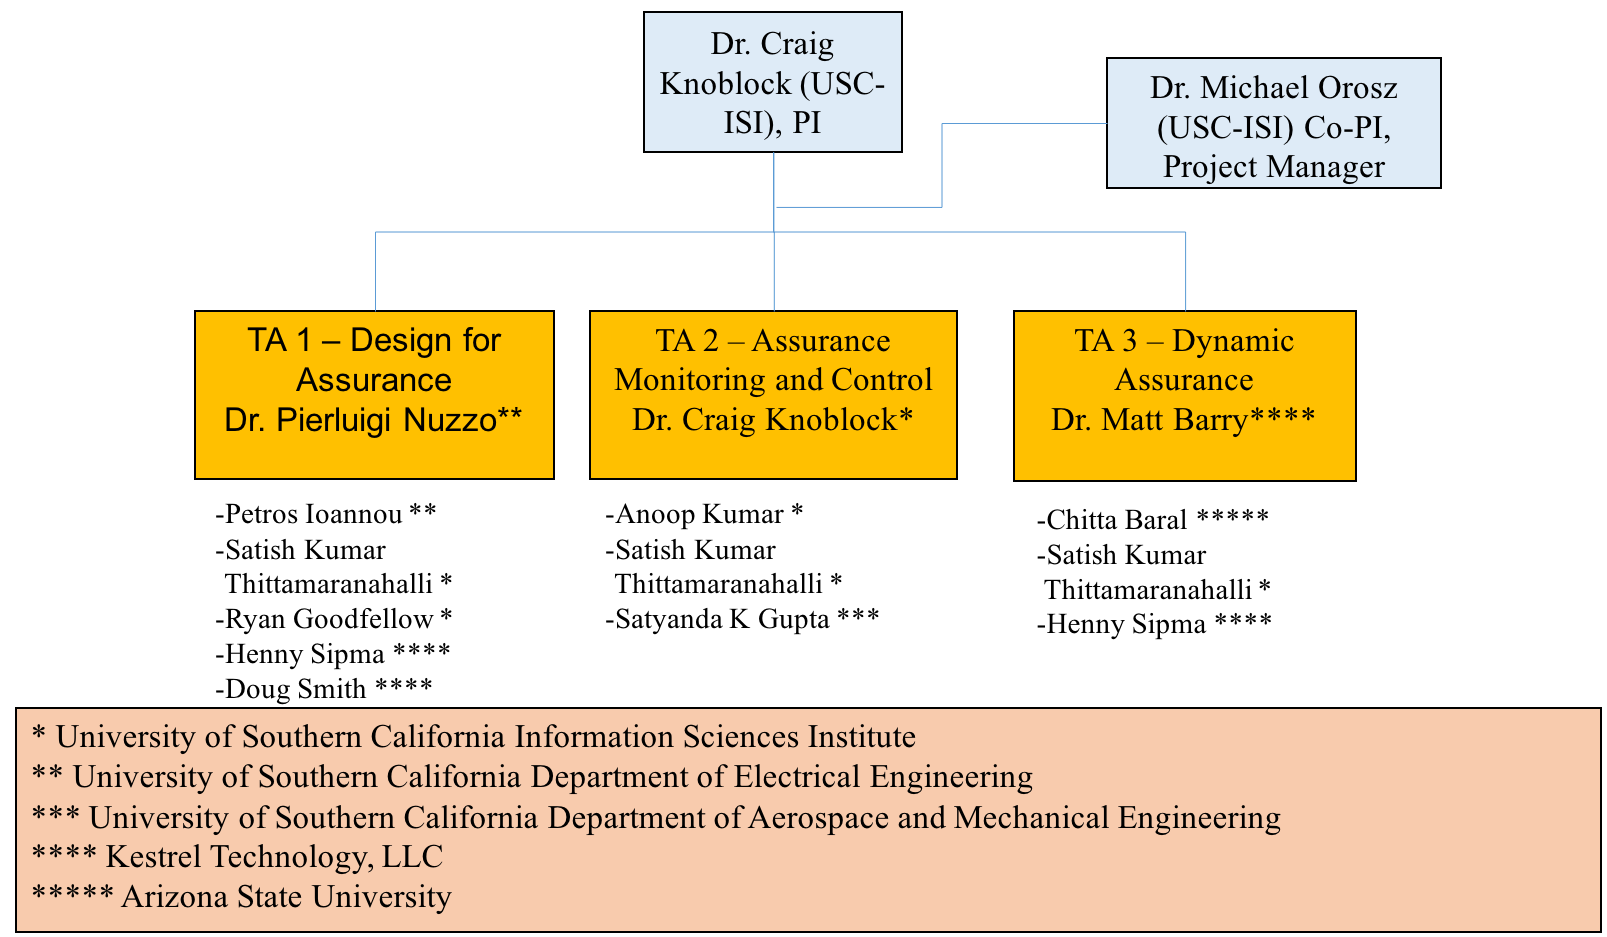
\includegraphics[width=6.0in]{./org-chart2.png}
\caption{\small Organization Chart}
\label{fig:org_chart}
\end{figure}

Coordination: To maximize collaboration and reduce risk to project failure from lack of communication and technical exchange, we plan to employ a wide variety of working styles and communication/coordination so that all can contribute.  At the core of our project will be regularly scheduled meetings bridging the diversely distributed team (Table~\ref{fig:Collaboration_Table}).  These meetings will address project status, identify challenges, implement risk mitigation strategies and participate in technology exchanges and system integration efforts (when appropriate)

\begin{table}[ht]
\caption{\small Project Meetings and Events}
  \centering
  {\footnotesize
\begin{tabular}{|m{3.15in}|m{3in}|} 
\hline
\textbf{Meeting} & \textbf{Frequency} 
\\\hline
Conference calls among investigators (discuss project status, address concerns and project risks) & Weekly
\\
\hline
Technical exchange and coordination meetings using Bluejeans or another videoconference technology & At least twice a month and more frequently as needed
  \\ 
\hline
Face-to-Face meetings (prior to P/I and demonstration meetings) & Every 3 to 6 months and more frequently (especially at the beginning of the project) as needed
 \\\cline{1-2}

\hline
\end{tabular}
}
\label{fig:Collaboration_Table}
\end{table}

\begin{table}[tbhp]
\caption{\small Key Project Team Member Responsibilities}
  \centering
  {\footnotesize
\begin{tabular}{| m{.75in} | m{3.9in}| m{1.5in}|} 
\hline
\textbf{Key Member} & \textbf{Responsibilities} & \textbf{Tasks} 
\\\hline
Dr.\ Craig Knoblock  & Principal Investigator responsible for project, leads TA 2 – Assurance Monitoring and Control.  Will lead the overall project and lead the TA2 team.  Served as the PI on many DARPA projects and has sucessfully led many large teams.    Effort on project:  25\% &
1.1.6, 1.2.2 1.2.3, 1.2.4, 1.3.4, 1.4.1, 
2.1.6, 2.2.2 2.2.3, 2.2.4, 2.3.4, 2.4.1, 
3.1.6, 3.2.2, 3.2.3, 3.2.4, 3.3.4, 3.4.1
\\
\hline
Dr.\ Michael Orosz & Co-Principal Investigator responsible managing the day-to-day operations of the project, assist technical teams as needed, coordinate with TA4 teams.    Has led many large complex multi-disciplined/multi-organizational projects in academic and industry environments.  Effort on project: 50\%
& 1.1.6, 2.1.6, 3.1.6, 1.4.1, 2.4.1, 3.4.1
  \\ 
\hline
Dr.\ Pierluigi Nuzzo 
& 
Co-Principal Investigator.  Leads the TA 1 - Design for Assurance team and conducts research on the formal methods for the design of the TA1 system.  Research experience on methodologies and tools for the design of cyber-physical systems; contracts, interfaces, and compositional methods for embedded system design; the application of automated formal methods and optimization theory to problems in embedded and cyber-physical systems.  Effort on project: 2 months/year (16.6\%)
& 
1.1.1, 2.1.1, 3.1.1 \\
\hline
Dr.\ Matthew Barry
& 
Key personnel.  Leads the TA 3 – Dynamic Assurance.   He will conduct the research on the dynamic assurance case language editors and parsers, the run-time system, and system integrations. Effort on project:  66\%
& 
1.3.2, 2.3.2, 3.3.2\\
\hline
Dr.\ Chitta Baral
& 
Key personnel responsible for learning assurance rules, supporting assurance rules with uncertainty and improving solver speed.  Expertise on ASP solvers, which will be used to reason about the assurance cases. Effort on project: 20\%
& 
1.3.1, 2.3.1, 3.3.1 \\
\hline
Dr.\ Doug Smith 
& 
Key personnel will support formal methods aspects of TA1, and lead the effort on abstract refinement. Expertise in field of automated correct-by-construction program generation.    Effort on project: 40\%
& 
1.1.5, 2.1.5, 3.1.5 \\
\hline
Dr.\ Henny Sipma
& 
Key personnel who will support the program verification tasks under TA1.  Will lead the effort on program verification.   Effort on project:  45\%
& 
1.1.5, 2.1.5, 3.1.5, 1.3.2, 2.3.2, 3.3.2 \\
\hline
Dr.\ Petros Ioannou
& 
Key personnel responsible providing and extending the assurance test bed, which will be available at the start of the project for autonomous vehicles.   Effort on project: 1 month/year (8.3\%)
& 
1.1.2, 2.1.2 (optional), 3.1.2 (optional)
\\
\hline
Dr.\ Satyandra Kumar Gupta
& 
Key Personnel providing autonomous command and control expertise to the TA-2 team.   Will lead the research on safety aware learning on TA2.   Past research on physics-aware decision making to facilitate automation.  Effort on project: 1 month/year (8.3\%)
& 
1.2.1, 2.2.1, 3.2.1 \\
\hline
Dr.\ Anoop Kumar 
& 
Key personnel providing support to the TA 2 project team.  Will lead the research on monitoring \& control and detecting distribution shifts.  Effort on project: 50\%
& 
1.2.1, 1.2.2, 1.2.3, 1.2.4, 2.2.1, 2.2.2, 2.2.3, 2.2.4, 3.2.1, 3.2.2, 3.2.3, 3.2.4\\
\hline
Dr.\ Satish Thittamaranahalli
& 
Key personnel developing scalable algorithms for TA1, TA2, and TA3 project teams.  Has extensive experience on scalable algorithm design, machine learning, and constraint reasoning.  Effort on project: 50\%
& 
1.2.1, 1.2.2, 1.2.3, 1.2.4, 2.2.1, 2.2.2, 2.2.3, 2.2.4, 3.2.1, 3.2.2, 3.2.3, 3.2.4, 1.1.4, 2.1.4, 3.1.4 \\
\hline
Dr.\ Ryan Goodfellow
& 
Key personnel providing support to the TA-1 project. Will lead the research on simulation-based testing.  Has extensive experience on simulation-based testing.  Effort on project:  30\%
& 
1.1.3, 2.1.3, 3.1.3 \\

\cline{1-2}

\hline
\end{tabular}
}
\label{fig:Table_Mgmt}
\end{table}



\newpage
\section{Personnel, Qualifications and Commitment}

{\bf Dr.\ Craig Knoblock}, the PI on this effort, is a Research Professor of both Computer Science and Spatial Sciences at the University of Southern California (USC) and Director of the Intelligent Systems Division at the USC Information Sciences Institute.   He received his Ph.D. from Carnegie Mellon University in computer science. 
%His research focuses on techniques for describing, acquiring, and exploiting the semantics of data.  
In previous projects he has worked on developing  scalable approaches to execution monitoring, accurate detection of sensor failures, and   automatic modeling and reconstruction of sensors.  He has published more than 300 journal articles, book chapters, and conference papers on these topics.  Dr. Knoblock is a Fellow of the Association for the Advancement of Artificial Intelligence (AAAI), a Distinguished Scientist of the Association of Computing Machinery (ACM), a Senior Member of IEEE, past President and Trustee of the International Joint Conference on Artificial Intelligence.
%and winner of the 2014 Robert S. Engelmore Award.  

{\bf Dr.\ Michael Orosz}, a Co-PI on this effort, is a Research Associate Professor of Civil and Environmental Engineering at the University of Southern California (USC) and Research Director of the Decision Systems Group at the USC Information Sciences Institute.  Dr. Orosz has over 30 years’ experience in commercial and government software development, basic and applied research, project management, academic research and has developed and deployed several commercially successful products.  His research interests are in machine learning and decision analytics as applied to intelligence analysis and autonomous command and control such as smart building controls.    Dr. Orosz has extensive experience in managing large complex multi-disciplined/multi-teamed research projects. %funded by DARPA, DHS, DoD, DoE, Industry, NASA, NRO, NSA and ONR.   
He received his Ph.D. in computer science from the University of California, Los Angeles.

{\bf Dr.\ Pierluigi Nuzzo}, a Co-PI on this project, is an Assistant Professor in the Department of Electrical Engineering at the University of Southern California. He received the Ph.D. in Electrical Engineering and Computer Sciences from the University of California at Berkeley. 
%in 2015, and the Laurea degree (MS) in electrical engineering (summa cum laude) from the University of Pisa, Italy, and the Sant'Anna School of Advanced Studies, Pisa, Italy.
%
%He has four years of research experience in analog and mixed signal circuit design as a researcher at IMEC, Leuven, Belgium, and over 10 years experience in design methodologies and tools for mixed-signal integrated circuits and cyber-physical systems, as a researcher at the University of Pisa, IMEC, UC Berkeley, and USC. 
His research interests
include: methodologies and tools for cyber-physical system and mixed-signal
system design; contracts, interfaces and compositional methods for embedded
system design; the application of formal methods and optimization theory to problems in embedded and cyber-physical systems and electronic design automation. 
%
Prof. Nuzzo received %First Place in the operational category and Best Overall
%Submission in the 2006 DAC/ISSCC Design Competition, 
a Marie Curie Fellowship
from the European Union in 2006, 
the University of California at Berkeley EECS
departmental fellowship in 2008, 
%the University of California at Berkeley Outstanding Graduate Student Instructor Award in 2013, 
the IBM Ph.D.
Fellowship in 2012 and 2014, 
%the Best Paper Award from the International Conference on Cyber-Physical Systems (ICCPS) in 2016, 
and the David J.~Sakrison Memorial Prize in 2016 for his doctoral research. 
%He is an author of 1 patent and over 60 publications.

{\bf Dr.\ Satyandra K. Gupta} is Smith International Professor in the Department of Aerospace and Mechanical Engineering at the University of Southern California. %Prior to joining the University of Southern California, he was a Professor in the Department of Mechanical Engineering and the Institute for Systems Research at the University of Maryland. He was the founding director of the Maryland Robotics Center and the Advanced Manufacturing Laboratory at the University of Maryland. 
He served as a program director for the National Robotics Initiative at the National Science Foundation from September 2012 to September 2014.  Dr. Gupta's interest is in the area of physics-aware decision making to facilitate automation. He has published more than 300 technical articles. He is a fellow of the American Society of Mechanical Engineers (ASME) and editor of ASME Journal of Computing and Information Science in Engineering. Dr. Gupta has received the Young Investigator Award from the Office of Naval Research in 2000, CAREER Award from the National Science Foundation in 2001, Presidential Early Career Award for Scientists and Engineers (PECASE) in 2001, Invention of the Year Award at the University of Maryland in 2007, Kos Ishii-Toshiba Award from ASME in 2011, and Excellence in Research Award from ASME in 2013.%, and Distinguished Alumnus Award from Indian Institute of Technology, Roorkee in 2014. %He has also received seven best paper awards at conferences.

{\bf Ryan Goodfellow} is a computer scientist at ISI working in combined cyber physical simulation and emulation platform development. His formal background is in simulation algorithms and modeling techniques using differential-algebraic equations (DAE). He has applied this knowledge in the CPS space by integrating DAE modeling languages and simulation engines with network testbeds to create comprehensive scientific experimentation platforms for cyber-physical systems. These experimentation platforms have been used in the power grid research space. %Ryan is a lead developer on the Deter network testbed, with a strong background in networked and distributed systems engineering. %He is also a combat veteran, serving as a non-commissioned officer and SIGINT team lead for a multi-functional intelligence team in Afghanistan.

{\bf Dr.\ Petros Ioannou} is a Professor in the Department of Electrical Engineering, Director of the Center for Advanced Transportation Technologies and Associate Director for Research for the DOT supported University Transportation Center at USC. He received his MS and PhD from the University of Illinois at Urbana Champaign in Mechanical and Electrical Engineering, respectively. His research interests are in robust adaptive control, vehicle dynamics and control, human factors and safety, automated vehicles, nonlinear systems and Intelligent transportation Systems.  He received the 2016 IEEE Transportation Technologies field award and the 2016 IEEE Control system society Transition to Practice Award. He is a Fellow of IEEE, IFAC and IET and author/coauthor of 8 books and over 400 papers.

{\bf Dr.\ Matthew Barry} will serve as lead for the TA3 tasks. %He will implement the dynamic assurance case language editors and parsers, the run-time system, and system integrations.  He will implement the assurance case arguments and the API for updating argument structure and content.  
Dr. Barry currently is CEO at Kestrel Technology LLC, and previously spent 20 years in NASA space mission operations at the Jet Propulsion Lab and Johnson Space Center.  At NASA Headquarters he led the introduction of dependability case requirements and plans for flight computing systems in upcoming manned space exploration missions, as well as the development of Agency-level software-related safety-critical control system requirements.  He recently served as a Principal Investigator on DHS/Cyber S\&T STAMP (Static Tool Analysis Modernization Program), DARPA CSFV (Crowd Sourced Formal Verification), three NASA Aeronautics R\&D projects, and the AFRL-sponsored Static Analysis of Numerical Algorithms project.  Dr. Barry earned BSME, MS, and PhD degrees in mechanical engineering, and an MBA degree, from Rice University.  

{\bf Dr.\ Henny Sipma} will support the program verification tasks under TA1.  %She is the key person behind the company's {\em KT Advance\/} and {\em KT Transferal\/} static analysis products, and the designer and programmer of the company's core {\em CodeHawk\/} abstract interpretation engine. 
Dr. Sipma currently is the CTO at Kestrel Technology LLC.  She has spent the past 10 years with Kestrel Technology as a static analysis expert; previously developed and taught static analysis techniques as senior research associate at Stanford University for eight years; and developed industrial process controls as an senior systems analyst at Shell.  She has been Principal Investigator or company lead on several recent R\&D projects for Federal agencies, including two projects under the IARPA STONESOUP (Securely Taking On New Executable Software of Uncertain Provenance) program; the DHS Cyber S\&T Gold Standard project; and the DARPA-sponsored STAC (Space-Time Analysis for Cybersecurity) and MUSE (Mining and Understanding Software Enclaves) programs.  Dr. Sipma earned 
%a BS degree in chemistry and an MS degree in chemical engineering at the University of Groningen in The Netherlands, and 
MS and PhD degrees in computer science from Stanford University.  

{\bf Dr.\ Douglas R.\ Smith} will support formal methods aspects of TA1, including the enforcement of safety properties and the generation of monitors.  He is President of Kestrel Technology LLC and Principal Scientist at Kestrel Institute.  He is a Fellow of the American Association of Artificial Intelligence (AAAI) and an ASE Fellow (Automated Software Engineering).  From 1986 to 2000, he taught an advanced graduate course on correct-by-construction software development at Stanford.  
%Dr. Smith has led the development of a series of software synthesis systems, including KIDS (Kestrel Interactive Development System), Specware, Designware, and Planware. 
%Applications domains have included a variety of complex high-performance planners and schedulers for the US Air Force.  He leads current projects on the generation of air mission plans and cyberoperations.  
Other recent projects focused on automated policy enforcement \cite{SmithD0703,SmithD08}, synthesis of secure network protocol codes, and the synthesis of high-performance constraint-solvers\cite{SmithD08c,SmithD13}.  Dr. Smith has over 30 years experience in the field of automated correct-by-construction program generation and has published over 100 papers. He has one patent.  He received the Ph.D. in Computer Science from Duke University% in 1979.  

{\bf Dr. Chitta Baral} is a Professor in the Department of Computer Science and Engineering at Arizona State University. He will support the TA3 efforts on Learning assurance rules, supporting assurance rules with uncertainty and improving solver speed. Dr. Baral has expertise in various aspects of autonomy and Artificial Intelligence. 
He wrote the first book on answer set programming (published by Cambridge University Press) the formal language behind our assurance rules. Some of his other works relevant to this proposal are: goal specification for autonomous systems, automatic construction of control rules for autonomous systems that satisfy given goals, combining machine learning with reasoning in various contexts, including image understanding. %He is the President of KR Inc. He is an associate editor of AIJ and has been an associate editor of JAIR.

{\bf Dr.\ Satish Kumar Thittamaranahalli (T. K. Satish Kumar)} leads the Collaboratory for Algorithmic Techniques and Artificial Intelligence (CATAI) at USC's Information Sciences Institute. He has published over 60 papers on numerous topics in Artificial Intelligence spanning such diverse areas as Constraint Reasoning, Planning and Scheduling, Probabilistic Reasoning, Robotics, Combinatorial Optimization, Approximation and Randomization, Heuristic Search, Model-Based Reasoning, Knowledge Representation and Spatio-Temporal Reasoning. %He %has served on the Program Committees of many international conferences in Artificial Intelligence
He and is a winner of the 2016 Best Robotics Paper Award and the 2005 Best Student Paper Award from the International Conference on Automated Planning and Scheduling. 
Dr. Kumar received his PhD in Computer Science from Stanford University. %In the past, he has also been a Visiting Student at the NASA Ames Research Center, a Postdoctoral Research Scholar at the University of California, Berkeley, a Research Scientist at the Institute for Human and Machine Cognition, a Visiting Assistant Professor at the University of West Florida, and a Senior Research and Development Scientist at Mission Critical Technologies.

\textbf{Dr.\ Anoop Kumar} is a senior computer scientist at USC ISI and has broad expertise in machine learning, statistical modeling, and software engineering.  Dr.\ Kumar is the technical lead on the DARPA RSPACE program and has played a vital role in developing a system that fuses air operations data from multiple sources, maintains world state, and issues warnings. Previously, he led the research and development of the BBN’s election forecasting system for the IARPA OSI program. %Dr.\ Kumar played a significant role in the DARPA DEFT program by developing a model to support integration of output from multiple NLP algorithms. He has contributed at the development to management levels on government research contracts and commercial projects. 
Dr.\ Kumar helped design and develop BBN's commercially available, hosted speech and medical transcription services offering. 

\begin{table}[!tbh]
\begin{footnotesize}
\vspace{-0.1in}

\begin{tabular}{lll}
\begin{tabular}[t]{|l|@{}c@{}|@{}c@{}|@{}c@{}|@{}c@{}|} \hline
Project & Status & \multicolumn{3}{ c| }{Hours} \\ \cline{3-5}
& & P1 & P2 & P3 \\ \hline



\multicolumn{5}{ |c| }{ \textbf{Craig Knoblock} } \\ \cline{1-5}
Safeguard & Pro & 770 & 641 & 641 \\ \cline{1-5}
ELICIT & Cur & 308 & 256 & 120 \\ \cline{1-5}
WTNIC & Cur & 11 & 0 & 0 \\ \cline{1-5}
EFFECT & Cur & 641 & 107 & 0 \\ \cline{1-5}
LinkedMaps & Cur & 203 & 25 & 0 \\ \cline{1-5}
PRINCESS & Cur & 608 & 96 & 0 \\ \cline{1-5}
SCHARP & Cur & 481 & 54 & 0 \\ \cline{1-5}
MINT & Pen & 650 & 534 & 285 \\ \cline{1-5}

\multicolumn{5}{ |c| }{ \textbf{Michael Orosz} } \\ \cline{1-5}
Safeguard & Pro & 1560 & 1300 & 1300  \\ \cline{1-5}
SMC/SY & Cur & 1803 & 0 & 0  \\ \cline{1-5}

\multicolumn{5}{ |c| }{ \textbf{Matthew Barry} } \\ \cline{1-5}
Safeguard & Pro & 2078 & 1690 & 1554 \\ \cline{1-5}
Starlite & Cur & 1840 & 1692 & 0 \\ \cline{1-5}



\multicolumn{5}{ |c| }{ \textbf{Anoop Kumar} } \\ \cline{1-5}
Safeguard & Pro & 1560 & 1300 & 1300 \\ \cline{1-5}

\end{tabular}
&
\begin{tabular}[t]{|l|@{}c@{}|@{}c@{}|@{}c@{}|@{}c@{}|} \hline
Project & Status & \multicolumn{3}{ c| }{Hours} \\ \cline{3-5}
& & P1 & P2 & P3 \\ \hline

\multicolumn{5}{ |c| }{ \textbf{Pierluigi Nuzzo} } \\ \cline{1-5}
Safeguard & Pro & 520 & 433 & 433  \\ \cline{1-5}
Mirage & Cur & 433 & 0 & 0  \\ \cline{1-5}

\multicolumn{5}{ |c| }{ \textbf{Satyandra Gupta} } \\ \cline{1-5}
Safeguard & Pro & 260 & 217 & 217 \\ \cline{1-5}
Human   & Cur & 22 & 0 & 0 \\ \cline{1-5}
Vehicles & Cur & 36 & 0 & 0 \\ \cline{1-5}
Robot & Cur & 116 & 0 & 0 \\ \cline{1-5}
Assembly & Cur & 33 & 0 & 0 \\ \cline{1-5}
Solar & Cur & 4 & 0 & 0 \\ \cline{1-5}

\multicolumn{5}{ |c| }{ \textbf{Petros Ioannou} } \\ \cline{1-5}
Safeguard & Pro & 260 & 217 & 217 \\ \cline{1-5}
CPS & Cur & 130 & 0 & 0 \\ \cline{1-5}

\multicolumn{5}{ |c| }{ \textbf{Ryan Goodfellow} } \\ \cline{1-5}
Safeguard & Pro & 936 & 780 & 780 \\ \cline{1-5}
STEAM & Cur & 416 & 0 & 0 \\ \cline{1-5}


\end{tabular}
&
\begin{tabular}[t]{|l|@{}c@{}|@{}c@{}|@{}c@{}|@{}c@{}|} \hline
Project & Status & \multicolumn{3}{ c| }{Hours} \\ \cline{3-5}
& & P1 & P2 & P3 \\ \hline

\multicolumn{5}{ |c| }{ \textbf{Chitta Baral} } \\ \cline{1-5}
Safeguard & Pro & 659 & 485 & 485 \\ \cline{1-5}
PostdocBP & Cur & 176 & 0 & 0 \\ \cline{1-5}
Languages & Pen & 528 & 264 & 264 \\ \cline{1-5}
CAREER & Pen & 88 & 44 & 44 \\ \cline{1-5}
CHS & Pen & 510 & 255 & 0 \\ \cline{1-5}

\multicolumn{5}{ |c| }{ \textbf{Doug Smith} } \\ \cline{1-5}
Safeguard & Pro & 1222 & 984 & 840 \\ \cline{1-5}
RSPACE & Cur & 342 & 0 & 0 \\ 
\cline{1-5}
PLANX & Cur & 154 & 0 & 0 \\ 
\cline{1-5}
HACCS & Pen & 923 & 769 & 769 \\ 
\cline{1-5}

\multicolumn{5}{ |c| }{ \textbf{Henny Sipma} } \\ \cline{1-5}
Safeguard & Pro & 1372 & 962 & 840 \\ \cline{1-5}
STAC & Cur & 797 & 0 & 0 \\ \cline{1-5}

\multicolumn{5}{ |c| }{ \textbf{Satish Thittamaranahalli} } \\ \cline{1-5}
Safeguard & Pro & 1560 & 1300 & 1300 \\ \cline{1-5}
MapF & Cur & 103 & 103 & 0 \\ \cline{1-5}

\end{tabular}
\end{tabular}

\end{footnotesize}
\caption{Individual commitments of key personnel}
\label{tab:Commitments}
\vspace{-0.2in}
\end{table}

\clearpage
\newpage
\section{Capabilities}


%\subsection{University of Southern California}
USC has strengths in number of areas that are closely related to the proposed work:
\begin{itemize}[itemsep=0pt,leftmargin=*]
\item Dr.\ Nuzzo 
%has over 10-year research experience in embedded system design, from mixed-signal chip design (analog-to-digital converters, frequency synthesizers, software-defined radio), to methodologies and tools for mixed-signal integrated circuits and Cyber-Physical Systems (CPSs), and the application of formal methods and optimization theory to problems in embedded and cyber-physical systems and electronic design automation.  
%His doctoral work 
has done extensive research on contracts and compositional methods for heterogeneous system design and design space exploration, with application to aircraft electric power systems and environmental control systems. His work has helped transition rigorous system design foundations, innovative design methodologies, and new systems engineering paradigms to industry (IBM, United Technologies). 
\item Dr.\ Satyandra K. Gupta has worked on autonomous surface vehicles, autonomous ground vehicles for operation on rugged terrains, and autonomous flapping wing aerial vehicles.   His group has developed a hierarchal decision making approach for realizing autonomous systems. 
%This approach combines task planning and assignment, deliberative trajectory planning, reactive collision avoidance behaviors, and trajectory tracking control layers. 
His group has also developed new methods for learning reactive behaviors in adversarial environments and COLREGS compliant trajectory planning. \item Dr.\ Knoblock has developed methods that learn the relationships between sensors to both identify failures and changes in sensor and reconstruct those sensors, providing estimates of the accuracy of the reconstructed sensors.  
\item Ryan Goodfellow has extensive experience in simulation based testing through high-fidelity CPS testbed environment development and operation, using the Deter network testbed as the core which has supported several large scale government projects from a variety of agencies and thousands of users. %we have developed sophisticated CPS experiments under programs such as NFS RIPS, NIST SmartCities and the DHS Cybersecurity showcase.
\item Dr.\ Ioannou %helped  design and implement adaptive cruise control systems in collaboration with Ford Motor Company, which was commercialized four years before any other company. He 
worked on several DOT funded projects on automated vehicles and intelligent highway systems where he demonstrated his vehicle control designs for safety and performance on actual automated vehicles in test trucks and I-15 highway.
\item Drs.\ Knoblock, Kumar, and Thittamaranahalli have developed highly scalable approaches for monitoring message traffic to identify potential problems and issue warnings and alerts. 
\item Dr. Thittamaranahalli has developed state-of-the-art methods for efficiently solving large-scale search and optimization problems. %These techniques will be applicable in TA2 for safety-aware learning and planning, in TA2 for assurance monitoring and control, and in TA3 for dynamic assessment of assurance cases.

\end{itemize}
%\subsection{Kestrel Technology LLC}

Kestrel Technology's strength is in program analysis, specifically static analysis of both source and binary targets.  The company performs applied R\&D and product development for a variety of static analysis applications  pivoting primarily on the abstract interpretation technique.  The company recently initiated development of program analysis applications using logical equivalence techniques. As a provider of verification evidence in the form of mathematical proofs, the company also has expertise in the design and development of assurance case arguments for high-integrity systems using such evidence. %The company is engaged in a partnership with Wind River Systems to develop program analysis tools for its embedded system developers.  Many of Wind River's customers must develop their products under safety and certification standards, including those using safety cases.  

   

%\subsection{Arizona State University}
Chitta Baral at Arizona State University has developed various software to learn assurance rules and various ASP solvers, which he has made available as open-source.

Most of the software carried forward for implementation or derivation is open source.  The single exception is Kestrel Technology's {\it KT Advance\/} static analysis tool (TA1), in particular the abstract interpretation engine therein, which is company proprietary and is US EAR export-controlled.   
%Owing to mixed funding for the development of that technology 
We will continue to provide the Federal government a restricted use license for that particular item.

There are no specialized facilities, data, or GFE required for this effort. 

\include{sow}
\include{milestones}

% \section{Level of Effort by Task \textcolor{red}{[Mike/Lisa - 1 pages]}}

% \textcolor{blue}{
% \begin{itemize}
% \item Will be a separate spreadsheet
% \item
% \end{itemize}
% }

\include{appendix_a}

%\section{Appendix B \textcolor{red}{[No Page Count]}}

\section{References}
\bibliographystyle{acm} 
\bibliography{TA3/ta3,TA2/ta2,TA1/ta1}
\end{document}
\clearpage
\newpage


\section{Management Plan}


The Principal Investigator for this effort is Dr. Craig Knoblock who is responsible for all aspects of the effort, will coordinate the parallel team efforts, and will ensure high levels of performance from individual team members.  The Co-P/I, Dr. Michael Orosz, will provide project management and will assist all performers in the execution of the project.    The project team is divided into three working groups (Figure~\ref{fig:org_chart}) corresponding to Technical Areas 1-3, however, members of each team contribute across all project activities.   Table~\ref{fig:Table_Mgmt} defines the major contributions of each project team member to the project tasks.

\begin{figure}[tbhp]
%\vspace{-25pt}
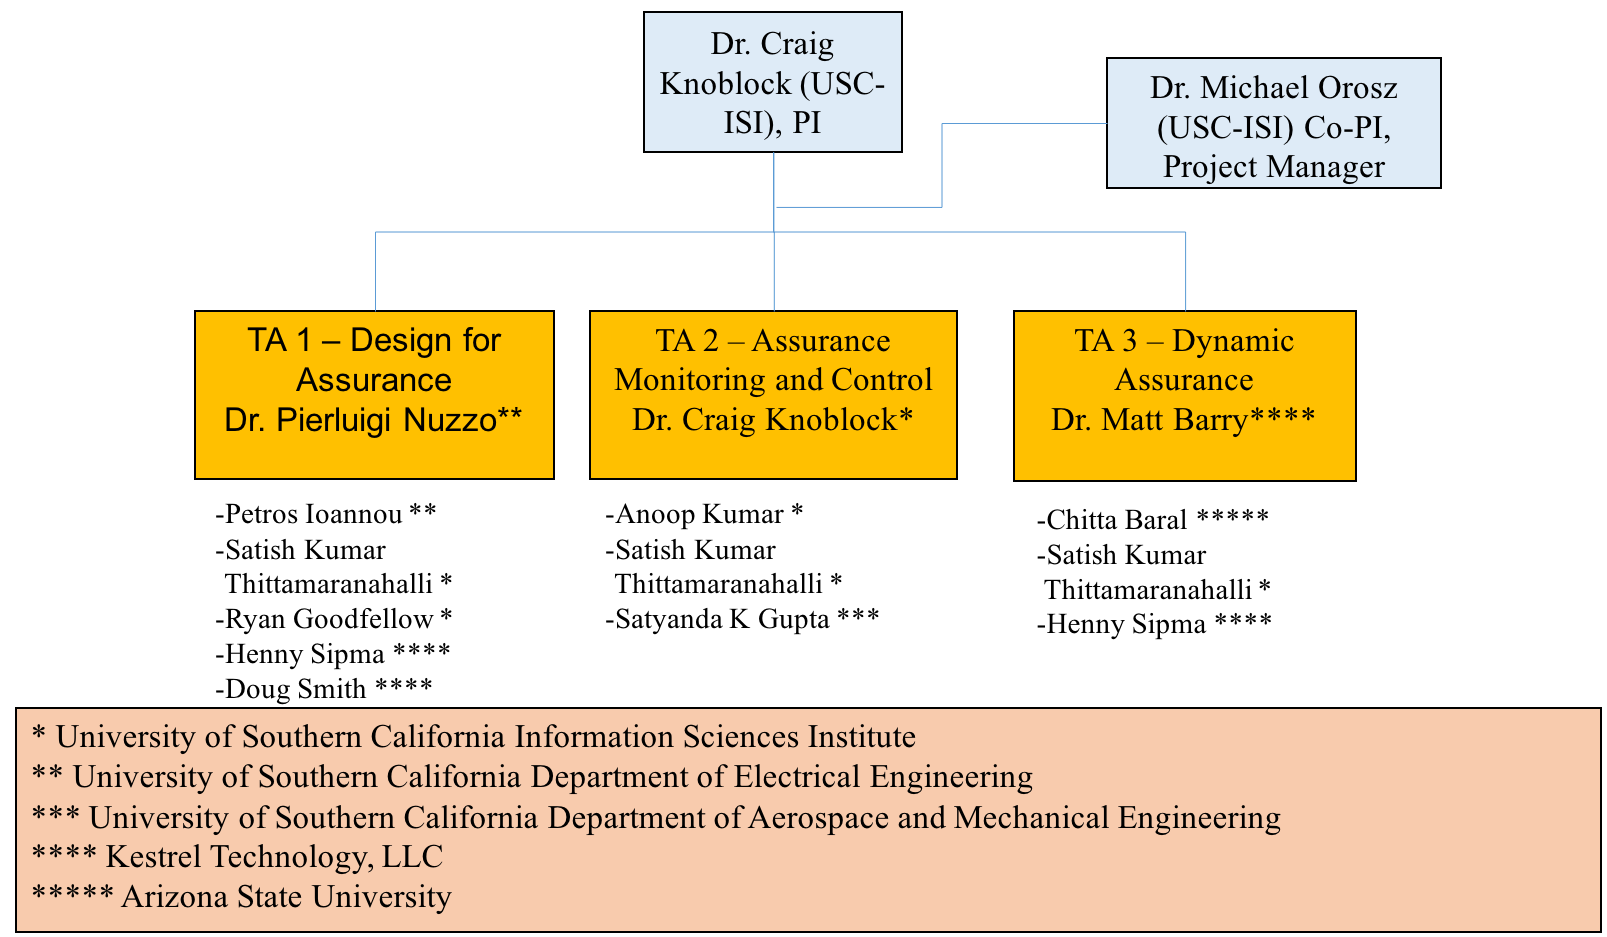
\includegraphics[width=6.0in]{./org-chart2.png}
\caption{\small Organization Chart}
\label{fig:org_chart}
\end{figure}

Coordination: To maximize collaboration and reduce risk to project failure from lack of communication and technical exchange, we plan to employ a wide variety of working styles and communication/coordination so that all can contribute.  At the core of our project will be regularly scheduled meetings bridging the diversely distributed team (Table~\ref{fig:Collaboration_Table}).  These meetings will address project status, identify challenges, implement risk mitigation strategies and participate in technology exchanges and system integration efforts (when appropriate)

\begin{table}[ht]
\caption{\small Project Meetings and Events}
  \centering
  {\footnotesize
\begin{tabular}{|m{3.15in}|m{3in}|} 
\hline
\textbf{Meeting} & \textbf{Frequency} 
\\\hline
Conference calls among investigators (discuss project status, address concerns and project risks) & Weekly
\\
\hline
Technical exchange and coordination meetings using Bluejeans or another videoconference technology & At least twice a month and more frequently as needed
  \\ 
\hline
Face-to-Face meetings (prior to P/I and demonstration meetings) & Every 3 to 6 months and more frequently (especially at the beginning of the project) as needed
 \\\cline{1-2}

\hline
\end{tabular}
}
\label{fig:Collaboration_Table}
\end{table}

\begin{table}[tbhp]
\caption{\small Key Project Team Member Responsibilities}
  \centering
  {\footnotesize
\begin{tabular}{| m{.75in} | m{3.9in}| m{1.5in}|} 
\hline
\textbf{Key Member} & \textbf{Responsibilities} & \textbf{Tasks} 
\\\hline
Dr.\ Craig Knoblock  & Principal Investigator responsible for project, leads TA 2 – Assurance Monitoring and Control.  Will lead the overall project and lead the TA2 team.  Served as the PI on many DARPA projects and has sucessfully led many large teams.    Effort on project:  25\% &
1.1.6, 1.2.2 1.2.3, 1.2.4, 1.3.4, 1.4.1, 
2.1.6, 2.2.2 2.2.3, 2.2.4, 2.3.4, 2.4.1, 
3.1.6, 3.2.2, 3.2.3, 3.2.4, 3.3.4, 3.4.1
\\
\hline
Dr.\ Michael Orosz & Co-Principal Investigator responsible managing the day-to-day operations of the project, assist technical teams as needed, coordinate with TA4 teams.    Has led many large complex multi-disciplined/multi-organizational projects in academic and industry environments.  Effort on project: 50\%
& 1.1.6, 2.1.6, 3.1.6, 1.4.1, 2.4.1, 3.4.1
  \\ 
\hline
Dr.\ Pierluigi Nuzzo 
& 
Co-Principal Investigator.  Leads the TA 1 - Design for Assurance team and conducts research on the formal methods for the design of the TA1 system.  Research experience on methodologies and tools for the design of cyber-physical systems; contracts, interfaces, and compositional methods for embedded system design; the application of automated formal methods and optimization theory to problems in embedded and cyber-physical systems.  Effort on project: 2 months/year (16.6\%)
& 
1.1.1, 2.1.1, 3.1.1 \\
\hline
Dr.\ Matthew Barry
& 
Key personnel.  Leads the TA 3 – Dynamic Assurance.   He will conduct the research on the dynamic assurance case language editors and parsers, the run-time system, and system integrations. Effort on project:  66\%
& 
1.3.2, 2.3.2, 3.3.2\\
\hline
Dr.\ Chitta Baral
& 
Key personnel responsible for learning assurance rules, supporting assurance rules with uncertainty and improving solver speed.  Expertise on ASP solvers, which will be used to reason about the assurance cases. Effort on project: 20\%
& 
1.3.1, 2.3.1, 3.3.1 \\
\hline
Dr.\ Doug Smith 
& 
Key personnel will support formal methods aspects of TA1, and lead the effort on abstract refinement. Expertise in field of automated correct-by-construction program generation.    Effort on project: 40\%
& 
1.1.5, 2.1.5, 3.1.5 \\
\hline
Dr.\ Henny Sipma
& 
Key personnel who will support the program verification tasks under TA1.  Will lead the effort on program verification.   Effort on project:  45\%
& 
1.1.5, 2.1.5, 3.1.5, 1.3.2, 2.3.2, 3.3.2 \\
\hline
Dr.\ Petros Ioannou
& 
Key personnel responsible providing and extending the assurance test bed, which will be available at the start of the project for autonomous vehicles.   Effort on project: 1 month/year (8.3\%)
& 
1.1.2, 2.1.2 (optional), 3.1.2 (optional)
\\
\hline
Dr.\ Satyandra Kumar Gupta
& 
Key Personnel providing autonomous command and control expertise to the TA-2 team.   Will lead the research on safety aware learning on TA2.   Past research on physics-aware decision making to facilitate automation.  Effort on project: 1 month/year (8.3\%)
& 
1.2.1, 2.2.1, 3.2.1 \\
\hline
Dr.\ Anoop Kumar 
& 
Key personnel providing support to the TA 2 project team.  Will lead the research on monitoring \& control and detecting distribution shifts.  Effort on project: 50\%
& 
1.2.1, 1.2.2, 1.2.3, 1.2.4, 2.2.1, 2.2.2, 2.2.3, 2.2.4, 3.2.1, 3.2.2, 3.2.3, 3.2.4\\
\hline
Dr.\ Satish Thittamaranahalli
& 
Key personnel developing scalable algorithms for TA1, TA2, and TA3 project teams.  Has extensive experience on scalable algorithm design, machine learning, and constraint reasoning.  Effort on project: 50\%
& 
1.2.1, 1.2.2, 1.2.3, 1.2.4, 2.2.1, 2.2.2, 2.2.3, 2.2.4, 3.2.1, 3.2.2, 3.2.3, 3.2.4, 1.1.4, 2.1.4, 3.1.4 \\
\hline
Dr.\ Ryan Goodfellow
& 
Key personnel providing support to the TA-1 project. Will lead the research on simulation-based testing.  Has extensive experience on simulation-based testing.  Effort on project:  30\%
& 
1.1.3, 2.1.3, 3.1.3 \\

\cline{1-2}

\hline
\end{tabular}
}
\label{fig:Table_Mgmt}
\end{table}



\newpage
\section{Personnel, Qualifications and Commitment}

{\bf Dr.\ Craig Knoblock}, the PI on this effort, is a Research Professor of both Computer Science and Spatial Sciences at the University of Southern California (USC) and Director of the Intelligent Systems Division at the USC Information Sciences Institute.   He received his Ph.D. from Carnegie Mellon University in computer science. 
%His research focuses on techniques for describing, acquiring, and exploiting the semantics of data.  
In previous projects he has worked on developing  scalable approaches to execution monitoring, accurate detection of sensor failures, and   automatic modeling and reconstruction of sensors.  He has published more than 300 journal articles, book chapters, and conference papers on these topics.  Dr. Knoblock is a Fellow of the Association for the Advancement of Artificial Intelligence (AAAI), a Distinguished Scientist of the Association of Computing Machinery (ACM), a Senior Member of IEEE, past President and Trustee of the International Joint Conference on Artificial Intelligence.
%and winner of the 2014 Robert S. Engelmore Award.  

{\bf Dr.\ Michael Orosz}, a Co-PI on this effort, is a Research Associate Professor of Civil and Environmental Engineering at the University of Southern California (USC) and Research Director of the Decision Systems Group at the USC Information Sciences Institute.  Dr. Orosz has over 30 years’ experience in commercial and government software development, basic and applied research, project management, academic research and has developed and deployed several commercially successful products.  His research interests are in machine learning and decision analytics as applied to intelligence analysis and autonomous command and control such as smart building controls.    Dr. Orosz has extensive experience in managing large complex multi-disciplined/multi-teamed research projects. %funded by DARPA, DHS, DoD, DoE, Industry, NASA, NRO, NSA and ONR.   
He received his Ph.D. in computer science from the University of California, Los Angeles.

{\bf Dr.\ Pierluigi Nuzzo}, a Co-PI on this project, is an Assistant Professor in the Department of Electrical Engineering at the University of Southern California. He received the Ph.D. in Electrical Engineering and Computer Sciences from the University of California at Berkeley. 
%in 2015, and the Laurea degree (MS) in electrical engineering (summa cum laude) from the University of Pisa, Italy, and the Sant'Anna School of Advanced Studies, Pisa, Italy.
%
%He has four years of research experience in analog and mixed signal circuit design as a researcher at IMEC, Leuven, Belgium, and over 10 years experience in design methodologies and tools for mixed-signal integrated circuits and cyber-physical systems, as a researcher at the University of Pisa, IMEC, UC Berkeley, and USC. 
His research interests
include: methodologies and tools for cyber-physical system and mixed-signal
system design; contracts, interfaces and compositional methods for embedded
system design; the application of formal methods and optimization theory to problems in embedded and cyber-physical systems and electronic design automation. 
%
Prof. Nuzzo received %First Place in the operational category and Best Overall
%Submission in the 2006 DAC/ISSCC Design Competition, 
a Marie Curie Fellowship
from the European Union in 2006, 
the University of California at Berkeley EECS
departmental fellowship in 2008, 
%the University of California at Berkeley Outstanding Graduate Student Instructor Award in 2013, 
the IBM Ph.D.
Fellowship in 2012 and 2014, 
%the Best Paper Award from the International Conference on Cyber-Physical Systems (ICCPS) in 2016, 
and the David J.~Sakrison Memorial Prize in 2016 for his doctoral research. 
%He is an author of 1 patent and over 60 publications.

{\bf Dr.\ Satyandra K. Gupta} is Smith International Professor in the Department of Aerospace and Mechanical Engineering at the University of Southern California. %Prior to joining the University of Southern California, he was a Professor in the Department of Mechanical Engineering and the Institute for Systems Research at the University of Maryland. He was the founding director of the Maryland Robotics Center and the Advanced Manufacturing Laboratory at the University of Maryland. 
He served as a program director for the National Robotics Initiative at the National Science Foundation from September 2012 to September 2014.  Dr. Gupta's interest is in the area of physics-aware decision making to facilitate automation. He has published more than 300 technical articles. He is a fellow of the American Society of Mechanical Engineers (ASME) and editor of ASME Journal of Computing and Information Science in Engineering. Dr. Gupta has received the Young Investigator Award from the Office of Naval Research in 2000, CAREER Award from the National Science Foundation in 2001, Presidential Early Career Award for Scientists and Engineers (PECASE) in 2001, Invention of the Year Award at the University of Maryland in 2007, Kos Ishii-Toshiba Award from ASME in 2011, and Excellence in Research Award from ASME in 2013.%, and Distinguished Alumnus Award from Indian Institute of Technology, Roorkee in 2014. %He has also received seven best paper awards at conferences.

{\bf Ryan Goodfellow} is a computer scientist at ISI working in combined cyber physical simulation and emulation platform development. His formal background is in simulation algorithms and modeling techniques using differential-algebraic equations (DAE). He has applied this knowledge in the CPS space by integrating DAE modeling languages and simulation engines with network testbeds to create comprehensive scientific experimentation platforms for cyber-physical systems. These experimentation platforms have been used in the power grid research space. %Ryan is a lead developer on the Deter network testbed, with a strong background in networked and distributed systems engineering. %He is also a combat veteran, serving as a non-commissioned officer and SIGINT team lead for a multi-functional intelligence team in Afghanistan.

{\bf Dr.\ Petros Ioannou} is a Professor in the Department of Electrical Engineering, Director of the Center for Advanced Transportation Technologies and Associate Director for Research for the DOT supported University Transportation Center at USC. He received his MS and PhD from the University of Illinois at Urbana Champaign in Mechanical and Electrical Engineering, respectively. His research interests are in robust adaptive control, vehicle dynamics and control, human factors and safety, automated vehicles, nonlinear systems and Intelligent transportation Systems.  He received the 2016 IEEE Transportation Technologies field award and the 2016 IEEE Control system society Transition to Practice Award. He is a Fellow of IEEE, IFAC and IET and author/coauthor of 8 books and over 400 papers.

{\bf Dr.\ Matthew Barry} will serve as lead for the TA3 tasks. %He will implement the dynamic assurance case language editors and parsers, the run-time system, and system integrations.  He will implement the assurance case arguments and the API for updating argument structure and content.  
Dr. Barry currently is CEO at Kestrel Technology LLC, and previously spent 20 years in NASA space mission operations at the Jet Propulsion Lab and Johnson Space Center.  At NASA Headquarters he led the introduction of dependability case requirements and plans for flight computing systems in upcoming manned space exploration missions, as well as the development of Agency-level software-related safety-critical control system requirements.  He recently served as a Principal Investigator on DHS/Cyber S\&T STAMP (Static Tool Analysis Modernization Program), DARPA CSFV (Crowd Sourced Formal Verification), three NASA Aeronautics R\&D projects, and the AFRL-sponsored Static Analysis of Numerical Algorithms project.  Dr. Barry earned BSME, MS, and PhD degrees in mechanical engineering, and an MBA degree, from Rice University.  

{\bf Dr.\ Henny Sipma} will support the program verification tasks under TA1.  %She is the key person behind the company's {\em KT Advance\/} and {\em KT Transferal\/} static analysis products, and the designer and programmer of the company's core {\em CodeHawk\/} abstract interpretation engine. 
Dr. Sipma currently is the CTO at Kestrel Technology LLC.  She has spent the past 10 years with Kestrel Technology as a static analysis expert; previously developed and taught static analysis techniques as senior research associate at Stanford University for eight years; and developed industrial process controls as an senior systems analyst at Shell.  She has been Principal Investigator or company lead on several recent R\&D projects for Federal agencies, including two projects under the IARPA STONESOUP (Securely Taking On New Executable Software of Uncertain Provenance) program; the DHS Cyber S\&T Gold Standard project; and the DARPA-sponsored STAC (Space-Time Analysis for Cybersecurity) and MUSE (Mining and Understanding Software Enclaves) programs.  Dr. Sipma earned 
%a BS degree in chemistry and an MS degree in chemical engineering at the University of Groningen in The Netherlands, and 
MS and PhD degrees in computer science from Stanford University.  

{\bf Dr.\ Douglas R.\ Smith} will support formal methods aspects of TA1, including the enforcement of safety properties and the generation of monitors.  He is President of Kestrel Technology LLC and Principal Scientist at Kestrel Institute.  He is a Fellow of the American Association of Artificial Intelligence (AAAI) and an ASE Fellow (Automated Software Engineering).  From 1986 to 2000, he taught an advanced graduate course on correct-by-construction software development at Stanford.  
%Dr. Smith has led the development of a series of software synthesis systems, including KIDS (Kestrel Interactive Development System), Specware, Designware, and Planware. 
%Applications domains have included a variety of complex high-performance planners and schedulers for the US Air Force.  He leads current projects on the generation of air mission plans and cyberoperations.  
Other recent projects focused on automated policy enforcement \cite{SmithD0703,SmithD08}, synthesis of secure network protocol codes, and the synthesis of high-performance constraint-solvers\cite{SmithD08c,SmithD13}.  Dr. Smith has over 30 years experience in the field of automated correct-by-construction program generation and has published over 100 papers. He has one patent.  He received the Ph.D. in Computer Science from Duke University% in 1979.  

{\bf Dr. Chitta Baral} is a Professor in the Department of Computer Science and Engineering at Arizona State University. He will support the TA3 efforts on Learning assurance rules, supporting assurance rules with uncertainty and improving solver speed. Dr. Baral has expertise in various aspects of autonomy and Artificial Intelligence. 
He wrote the first book on answer set programming (published by Cambridge University Press) the formal language behind our assurance rules. Some of his other works relevant to this proposal are: goal specification for autonomous systems, automatic construction of control rules for autonomous systems that satisfy given goals, combining machine learning with reasoning in various contexts, including image understanding. %He is the President of KR Inc. He is an associate editor of AIJ and has been an associate editor of JAIR.

{\bf Dr.\ Satish Kumar Thittamaranahalli (T. K. Satish Kumar)} leads the Collaboratory for Algorithmic Techniques and Artificial Intelligence (CATAI) at USC's Information Sciences Institute. He has published over 60 papers on numerous topics in Artificial Intelligence spanning such diverse areas as Constraint Reasoning, Planning and Scheduling, Probabilistic Reasoning, Robotics, Combinatorial Optimization, Approximation and Randomization, Heuristic Search, Model-Based Reasoning, Knowledge Representation and Spatio-Temporal Reasoning. %He %has served on the Program Committees of many international conferences in Artificial Intelligence
He and is a winner of the 2016 Best Robotics Paper Award and the 2005 Best Student Paper Award from the International Conference on Automated Planning and Scheduling. 
Dr. Kumar received his PhD in Computer Science from Stanford University. %In the past, he has also been a Visiting Student at the NASA Ames Research Center, a Postdoctoral Research Scholar at the University of California, Berkeley, a Research Scientist at the Institute for Human and Machine Cognition, a Visiting Assistant Professor at the University of West Florida, and a Senior Research and Development Scientist at Mission Critical Technologies.

\textbf{Dr.\ Anoop Kumar} is a senior computer scientist at USC ISI and has broad expertise in machine learning, statistical modeling, and software engineering.  Dr.\ Kumar is the technical lead on the DARPA RSPACE program and has played a vital role in developing a system that fuses air operations data from multiple sources, maintains world state, and issues warnings. Previously, he led the research and development of the BBN’s election forecasting system for the IARPA OSI program. %Dr.\ Kumar played a significant role in the DARPA DEFT program by developing a model to support integration of output from multiple NLP algorithms. He has contributed at the development to management levels on government research contracts and commercial projects. 
Dr.\ Kumar helped design and develop BBN's commercially available, hosted speech and medical transcription services offering. 

\begin{table}[!tbh]
\begin{footnotesize}
\vspace{-0.1in}

\begin{tabular}{lll}
\begin{tabular}[t]{|l|@{}c@{}|@{}c@{}|@{}c@{}|@{}c@{}|} \hline
Project & Status & \multicolumn{3}{ c| }{Hours} \\ \cline{3-5}
& & P1 & P2 & P3 \\ \hline



\multicolumn{5}{ |c| }{ \textbf{Craig Knoblock} } \\ \cline{1-5}
Safeguard & Pro & 770 & 641 & 641 \\ \cline{1-5}
ELICIT & Cur & 308 & 256 & 120 \\ \cline{1-5}
WTNIC & Cur & 11 & 0 & 0 \\ \cline{1-5}
EFFECT & Cur & 641 & 107 & 0 \\ \cline{1-5}
LinkedMaps & Cur & 203 & 25 & 0 \\ \cline{1-5}
PRINCESS & Cur & 608 & 96 & 0 \\ \cline{1-5}
SCHARP & Cur & 481 & 54 & 0 \\ \cline{1-5}
MINT & Pen & 650 & 534 & 285 \\ \cline{1-5}

\multicolumn{5}{ |c| }{ \textbf{Michael Orosz} } \\ \cline{1-5}
Safeguard & Pro & 1560 & 1300 & 1300  \\ \cline{1-5}
SMC/SY & Cur & 1803 & 0 & 0  \\ \cline{1-5}

\multicolumn{5}{ |c| }{ \textbf{Matthew Barry} } \\ \cline{1-5}
Safeguard & Pro & 2078 & 1690 & 1554 \\ \cline{1-5}
Starlite & Cur & 1840 & 1692 & 0 \\ \cline{1-5}



\multicolumn{5}{ |c| }{ \textbf{Anoop Kumar} } \\ \cline{1-5}
Safeguard & Pro & 1560 & 1300 & 1300 \\ \cline{1-5}

\end{tabular}
&
\begin{tabular}[t]{|l|@{}c@{}|@{}c@{}|@{}c@{}|@{}c@{}|} \hline
Project & Status & \multicolumn{3}{ c| }{Hours} \\ \cline{3-5}
& & P1 & P2 & P3 \\ \hline

\multicolumn{5}{ |c| }{ \textbf{Pierluigi Nuzzo} } \\ \cline{1-5}
Safeguard & Pro & 520 & 433 & 433  \\ \cline{1-5}
Mirage & Cur & 433 & 0 & 0  \\ \cline{1-5}

\multicolumn{5}{ |c| }{ \textbf{Satyandra Gupta} } \\ \cline{1-5}
Safeguard & Pro & 260 & 217 & 217 \\ \cline{1-5}
Human   & Cur & 22 & 0 & 0 \\ \cline{1-5}
Vehicles & Cur & 36 & 0 & 0 \\ \cline{1-5}
Robot & Cur & 116 & 0 & 0 \\ \cline{1-5}
Assembly & Cur & 33 & 0 & 0 \\ \cline{1-5}
Solar & Cur & 4 & 0 & 0 \\ \cline{1-5}

\multicolumn{5}{ |c| }{ \textbf{Petros Ioannou} } \\ \cline{1-5}
Safeguard & Pro & 260 & 217 & 217 \\ \cline{1-5}
CPS & Cur & 130 & 0 & 0 \\ \cline{1-5}

\multicolumn{5}{ |c| }{ \textbf{Ryan Goodfellow} } \\ \cline{1-5}
Safeguard & Pro & 936 & 780 & 780 \\ \cline{1-5}
STEAM & Cur & 416 & 0 & 0 \\ \cline{1-5}


\end{tabular}
&
\begin{tabular}[t]{|l|@{}c@{}|@{}c@{}|@{}c@{}|@{}c@{}|} \hline
Project & Status & \multicolumn{3}{ c| }{Hours} \\ \cline{3-5}
& & P1 & P2 & P3 \\ \hline

\multicolumn{5}{ |c| }{ \textbf{Chitta Baral} } \\ \cline{1-5}
Safeguard & Pro & 659 & 485 & 485 \\ \cline{1-5}
PostdocBP & Cur & 176 & 0 & 0 \\ \cline{1-5}
Languages & Pen & 528 & 264 & 264 \\ \cline{1-5}
CAREER & Pen & 88 & 44 & 44 \\ \cline{1-5}
CHS & Pen & 510 & 255 & 0 \\ \cline{1-5}

\multicolumn{5}{ |c| }{ \textbf{Doug Smith} } \\ \cline{1-5}
Safeguard & Pro & 1222 & 984 & 840 \\ \cline{1-5}
RSPACE & Cur & 342 & 0 & 0 \\ 
\cline{1-5}
PLANX & Cur & 154 & 0 & 0 \\ 
\cline{1-5}
HACCS & Pen & 923 & 769 & 769 \\ 
\cline{1-5}

\multicolumn{5}{ |c| }{ \textbf{Henny Sipma} } \\ \cline{1-5}
Safeguard & Pro & 1372 & 962 & 840 \\ \cline{1-5}
STAC & Cur & 797 & 0 & 0 \\ \cline{1-5}

\multicolumn{5}{ |c| }{ \textbf{Satish Thittamaranahalli} } \\ \cline{1-5}
Safeguard & Pro & 1560 & 1300 & 1300 \\ \cline{1-5}
MapF & Cur & 103 & 103 & 0 \\ \cline{1-5}

\end{tabular}
\end{tabular}

\end{footnotesize}
\caption{Individual commitments of key personnel}
\label{tab:Commitments}
\vspace{-0.2in}
\end{table}

\clearpage
\newpage
\section{Capabilities}


%\subsection{University of Southern California}
USC has strengths in number of areas that are closely related to the proposed work:
\begin{itemize}[itemsep=0pt,leftmargin=*]
\item Dr.\ Nuzzo 
%has over 10-year research experience in embedded system design, from mixed-signal chip design (analog-to-digital converters, frequency synthesizers, software-defined radio), to methodologies and tools for mixed-signal integrated circuits and Cyber-Physical Systems (CPSs), and the application of formal methods and optimization theory to problems in embedded and cyber-physical systems and electronic design automation.  
%His doctoral work 
has done extensive research on contracts and compositional methods for heterogeneous system design and design space exploration, with application to aircraft electric power systems and environmental control systems. His work has helped transition rigorous system design foundations, innovative design methodologies, and new systems engineering paradigms to industry (IBM, United Technologies). 
\item Dr.\ Satyandra K. Gupta has worked on autonomous surface vehicles, autonomous ground vehicles for operation on rugged terrains, and autonomous flapping wing aerial vehicles.   His group has developed a hierarchal decision making approach for realizing autonomous systems. 
%This approach combines task planning and assignment, deliberative trajectory planning, reactive collision avoidance behaviors, and trajectory tracking control layers. 
His group has also developed new methods for learning reactive behaviors in adversarial environments and COLREGS compliant trajectory planning. \item Dr.\ Knoblock has developed methods that learn the relationships between sensors to both identify failures and changes in sensor and reconstruct those sensors, providing estimates of the accuracy of the reconstructed sensors.  
\item Ryan Goodfellow has extensive experience in simulation based testing through high-fidelity CPS testbed environment development and operation, using the Deter network testbed as the core which has supported several large scale government projects from a variety of agencies and thousands of users. %we have developed sophisticated CPS experiments under programs such as NFS RIPS, NIST SmartCities and the DHS Cybersecurity showcase.
\item Dr.\ Ioannou %helped  design and implement adaptive cruise control systems in collaboration with Ford Motor Company, which was commercialized four years before any other company. He 
worked on several DOT funded projects on automated vehicles and intelligent highway systems where he demonstrated his vehicle control designs for safety and performance on actual automated vehicles in test trucks and I-15 highway.
\item Drs.\ Knoblock, Kumar, and Thittamaranahalli have developed highly scalable approaches for monitoring message traffic to identify potential problems and issue warnings and alerts. 
\item Dr. Thittamaranahalli has developed state-of-the-art methods for efficiently solving large-scale search and optimization problems. %These techniques will be applicable in TA2 for safety-aware learning and planning, in TA2 for assurance monitoring and control, and in TA3 for dynamic assessment of assurance cases.

\end{itemize}
%\subsection{Kestrel Technology LLC}

Kestrel Technology's strength is in program analysis, specifically static analysis of both source and binary targets.  The company performs applied R\&D and product development for a variety of static analysis applications  pivoting primarily on the abstract interpretation technique.  The company recently initiated development of program analysis applications using logical equivalence techniques. As a provider of verification evidence in the form of mathematical proofs, the company also has expertise in the design and development of assurance case arguments for high-integrity systems using such evidence. %The company is engaged in a partnership with Wind River Systems to develop program analysis tools for its embedded system developers.  Many of Wind River's customers must develop their products under safety and certification standards, including those using safety cases.  

   

%\subsection{Arizona State University}
Chitta Baral at Arizona State University has developed various software to learn assurance rules and various ASP solvers, which he has made available as open-source.

Most of the software carried forward for implementation or derivation is open source.  The single exception is Kestrel Technology's {\it KT Advance\/} static analysis tool (TA1), in particular the abstract interpretation engine therein, which is company proprietary and is US EAR export-controlled.   
%Owing to mixed funding for the development of that technology 
We will continue to provide the Federal government a restricted use license for that particular item.

There are no specialized facilities, data, or GFE required for this effort. 


\section{Statement of Work}
We propose work for TA 1 – TA 3 for all three phases. All tasks span the four years of the program. For each task we provide an objective, the high-level approach (focusing on the responsibilities of each contributing organization), and the specific approach and milestones planned for each task for each phase. On all tasks, we will deliver design documents, software implementations, demonstrations, and publications. With the exception of several tasks accomplished by Kesler Technology, LLC, all tasks that accomplished at a university (USC/ISI, USC, and ASU) are believed to be fundamental research.   
%\usepackage[table]{xcolor}

{\scriptsize

\begin{longtable} {|p{\textwidth} | }

\hline

\textcolor{blue} {\footnotesize {\textbf{Tasks 1.1.1, 2.1.1, 3.1.1 -Design for Assurance System Models and Formal Verification (USC)}}} \\ \hline
Objective:  Develop contract-based formalisms and mapping tools to represent and reason about LE-CPSs at multiple levels of abstraction and generate assurance cases.  Undertake scalable formal verification and synthesis via Satisfiability Modulo Convex Programming. \\ \hline
Approach:  Develop modeling formalisms to represent components and contracts for LE-CPSs, including physical plant (e.g., autonomous vehicle, sensors, actuators, environment, controllers, and learning components. Formalisms will encompass different control and learning architectures (e.g., neural networks, statistical methods, graphical models, ensemble methods, decision trees) and support mapping between abstractions.   Develop a formal domain-specific language to capture and formalize requirements on LE components, systems, and their dynamics as contracts.   Develop a unifying framework and efficient algorithms to reason about the combination of discrete and continuous dynamics and constraints in the presence of uncertainties in LE cyber-physical systems \\ \hline
Phase 1 (1.1.1):  Milestone 1: Develop initial design followed by development and testing of individual components.  Milestone 2:  Library of components and contracts for the autonomous vehicle application driver.  Milestone 4: Library of components and contracts for the platforms provided by TA4 performers. Extension of the methodology and to support up to 20 continuous dimensions and 2 learning components for the 2 application drivers from TA4.  Milestone 6: -Prototype toolkit (software package) for capturing requirements, for translating them into contracts, for analyzing and validating them using contract operations and relations.  Prototype toolkit for capturing probabilistic requirements and behaviors of LE components, systems, and their dynamics, for translating them into stochastic assume-guarantee contracts, for analyzing and validating them using contract operations and relations, and for synthesizing design and verification artifacts from contracts.  Extension of the SMC framework and toolkit to support reactive and robust task and trajectory planning in the presence of uncertainties. \\ \hline
Phase 2 (2.1.1) Milestone 7: Refinement of design.  Milestone 9: extension of methodology, design, toolkits and libraries to support 40 continuous dimensions, 4 LECs, 30\% monitoring overhead. Extension of the SMC framework and toolkit from Phase 1 to support verification and synthesis on system with 40 dimensions and 4 LECs.  Milestone 10: Demonstration of the SMC framework and toolkit.  Contribution to Phase II report and dissemination of the results in conferences and journals. \\ \hline
Phase 3 (3.1.1) Milestone 11: Update design based on Phase II demo.  Milestones 12-13:  extend methodology, design, toolkits and libraries to support 100 dimensions, 6 LECs and 10\% monitoring overhead.   Milestone 14: Undertake Phase III demonstration on both platforms and submit final project report. \\ \hline
\textcolor{blue} {\footnotesize {\textbf{Tasks 1.1.2, 2.1.2, 3.1.2: Design for Assurance Testbed (USC)} }}\\ \hline
Objective:  Develop a simulation test bed for data generation and LE algorithm testing, redesign and/or refinement.   Simulator used as the test bed until the TA4 platforms are available.   Test bed will be used for internal research/prototype after TA4 platform availability. \\ \hline
Approach:  Leverage previous work on microscopic traffic simulations in urban and rural environments using the commercial software VISSIM and Vortex Studio and built in extensions for automated driving.   Develop testbed for autonomous vehicles in road/off-road environments to allow LEs to collect data, learn and make control decisions on line and in real time by simulating scenarios. The testbed together with analytical tools used to refine and redesign LEs and control algorithms by taking into account effects revealed by the simulation and not accounted for in the design stage.    In the event the TA4 platforms are not available, the test bed will be extended further by integrating all the LE components, controllers and sensors for demonstration purposes and evaluation of the proposed methodology. \\ \hline
Phase 1 (1.1.2):  Milestones 1-2:  Extension of existing simulator test beds.  Milestones 3-5:  Testing of individual components under normal and unpredicatble situations and demonstrating the results in VISSIM under several different driving scenarios. \\ \hline
Phase 2 (2.1.2) – Optional:  Milestones 7-8:  Extension of existing simulator test beds to support the TA1-TA3 teams.  Milestones 9-10:  Support demonstration of technology capable of supporting 40 dimensions, 4 LECs and 30\% monitoring overhead. \\ \hline
Phase 3 (3.1.2) – Optional:  Milestones 11-12:  Extension of existing simulator test beds to support the TA1-TA3 teams.  Milestones 13-14:  Support demonstration of technology capable of supporting 100 dimensions, 6 LECs and 10\% monitoring overhead. \\ \hline
\textcolor{blue} {\footnotesize {\textbf{Tasks 1.1.3, 2.1.3, 3.1.3: Design for Assurance Simulation Based Testing (USC/ISI)}}} \\ \hline
Objective:  Develop external Discrete Control Mechanisms for OpenModelica.  Develop/package virtual-machine based static time dilation systems. Undertake network testbed integration and develop physical system behavioral analysis tooling. \\ \hline
Approach:  Leverage previous external discrete control mechanisms for DAEs, implement similar facilities for OpenModelica to allow LEs to observe and control a physical system over a network. Contributions pushed back upstream to OpenModelica project.  Implement DieCast for modern libvirt.  Develop tooling to deploy integrated CPS models on the Deter network testbed. Apply modern DAE control theory in the form Modelica analysis packages usable by non DAE experts. \\ \hline
Phase 1 (1.1.3):  Milestones 1-2:  Initial CPS simulation concept and components.  Milestones 3-5:  Testing of individual components under normal and unpredictable situations and demonstrating the results capable of meeting 20 dimensions, 2 LECs and 50\% or under monitoring overhead conditions.   Milestone 6: Demonstrate technology in Phase I demonstration, contribute to Phase I final report and disseminate software and publications. \\ \hline
Phase 2 (2.1.3):  Milestones 7-8:  Apply lessons learned from Phase I and extend existing simulations to support 30 dimensions, 3 LECs and 40\% monitoring overhead.  Milestones 9-10:  Support demonstration of technology capable of supporting 40 dimensions, 4 LECs and 30\% monitoring overhead.  Contribute to Phase II final report and disseminate software and publications. \\ \hline
Phase 3 (3.1.3):  Milestones 11-12:  Apply lessons learned from Phase II and extend existing simulations to support 70 dimensions, 5 LECs and 20\% monitoring overhead.  Milestones 13-14:  Support demonstration of technology capable of supporting 100 dimensions, 6 LECs and 10\% monitoring overhead.  Contribute to Phase III final report and disseminate software and publications. \\ \hline
\textcolor{blue} {\footnotesize {\textbf{Tasks 1.1.4, 2.1.4, 3.1.4: Scalable Algorithms for Formal Verification (USC/ISI)}}} \\ \hline
Objective: Develop innovative algorithms for scalable formal verification. \\ \hline
Approach: Use state-of-the-art techniques for solving combinatorial problems with discrete/continuous variables and hybrid constraints. \\ \hline
Phase 1 (Task 1.1.4): Milestones 1-2: Develop initial design plan and initial concepts. Milestones 3-5: Integrate framework that is capable of supporting 20 dimensions, 2 LECs and 0.1x trials to assurance. Milestone 6: Participate in Phase I demonstration, contribute to Phase I final report and disseminate software and publications. \\ \hline
Phase 2 (Task 2.1.4): Milestones 7-8: Apply lessons learned from Phase I and extend existing design to support 30 dimensions, 3 LECs and 0.05x trials to assurance. Milestones 9-10: Demonstrate technology capable of supporting 40 dimensions, 4 LECs and 0.01x trials to assurance. Participate in Phase II demonstration, contribute to Phase II final report and disseminate software and publications. \\ \hline
Phase 3 (Task 3.1.4): Milestones 11-12: Apply lessons learned from Phase II and extend design/approach to support 70 dimensions, 5 LECs and 0.005x trials to assurance. Milestones 13-14: Demonstrate technology capable of supporting 100 dimensions, 6 LECs and 0.001x trials to assurance. Complete integration of technology into TA4 platform. Contribute to Phase III final report and disseminate software and publications. \\ \hline
\textcolor{blue} {\footnotesize {\textbf{Tasks 1.1.5, 2.1.5, 3.1.5: Design for Assurance Program Verification (Kestrel Technology, LLC)}}} \\ \hline
Objective: Develop and integrate program analysis and monitor synthesis functionality with TA1 functions and services and integrate combined TA1 functions with TA4 platform. \\ \hline
Approach: Integrate existing analysis tools into development environment.  Design and implement abstract domains and properties for one or more modeling layers.  Design and implement analyzer front-end for modeling layers.  Implement test framework for verification tools.  Implement content providers and/or consumers for DAC via DAC API.  Leverage existing algorithms and tools to generate monitors for assumptions and unproven safety constraints. Integrate program analysis and monitor synthesis functionality with TA1 functions and services, integrate combined TA1 functions with TA4 platform.   Prepare software and data installation kits and operating instructions;install software and confirm configuration. \\ \hline
Phase 1 (1.1.5) : Milestones 1-2:  Initial framework design and unit tools, TA1-TA3 interfaces defined. Milestones 3-5:  Testing of individual components/tools capable of meeting 20 dimensions, 2 LECs and 50\% or under monitoring overhead conditions.   Milestone 6: Demonstrate technology in Phase I demonstration, contribute to Phase I final report and disseminate software and publications. \\ \hline
Phase 2 (2.1.5): Milestones 7-8:  Apply lessons learned from Phase I and extend existing design to support 30 dimensions, 3 LECs and 40\% monitoring overhead.  Milestones 9-10:  Support demonstration of technology capable of supporting 40 dimensions, 4 LECs and 30\% monitoring overhead.  Contribute to Phase II final report and disseminate software and publications. \\ \hline
Phase 3 (3.1.5): Milestones 11-12:  Apply lessons learned from Phase II and extend existing simulations to support 70 dimensions, 5 LECs and 20\% monitoring overhead.  Milestones 13-14:  Support demonstration of technology capable of supporting 100 dimensions, 6 LECs and 10\% monitoring overhead.  Contribute to Phase III final report and disseminate software and publications. \\ \hline
\textcolor{blue} {\footnotesize {\textbf{Tasks 1.1.6, 2.1.6, 3.1.6: System integration, deployment, and testing (USC/ISI)}}} \\ \hline
Objective: Develop and implement integration, testing and deployment plan supporting TA1 for all three phases. \\ \hline
Approach: Develop an internal TA1 integration and testing plan (unit tests, etc.) and, in close collaboration with TA2 and TA3 performers on project, develop an overall TA1-TA3 integration and testing plan.  Working with TA4 performers, extend and execute plan for TA4 platform (when available). \\ \hline
Phase 1 (1.1.6): Milestones 1-2:  Develop initial integration and testing plan and implement on unit testing.  Milestones 3-5:  Oversee integration and testing of TA1-TA3 components for system capable of supporting 20 dimensions, 2 LECs and 50\% or less monitoring overhead.   Milestone 6: Complete integration of technology into TA4 testbeds, contribute to Phase I final report and disseminate software and publications. \\ \hline
Phase 2 (2.1.6): Milestones 7-8:  Apply lessons learned from Phase I and extend existing integration and testing plan to support 30 dimensions, 3 LECs and 40\% monitoring overhead.  Milestones 9-10:  Support demonstration of technology capable of supporting 40 dimensions, 4 LECs and 30\% monitoring overhead.  Complete integration of technology into TA4 platforms.  Contribute to Phase II final report and disseminate software and publications. \\ \hline
Phase 3 (3.1.6): Milestones 11-12:  Apply lessons learned from Phase II and extend existing integration and testing plan to support 70 dimensions, 5 LECs and 20\% monitoring overhead.  Milestones 13-14:  Support demonstration of technology capable of supporting 100 dimensions, 6 LECs and 10\% monitoring overhead.  Complete integration of technology into TA4 platform.  Contribute to Phase III final report and disseminate software and publications. \\ \hline
\textcolor{blue} {\footnotesize {\textbf{Tasks 1.2.1, 2.2.1, 3.2.1: Safety Aware Learning (USC)} }}\\ \hline
Objective: Enable the system to learn efficiently without violating safety constraints. \\ \hline
Approach: Integrate LECs with search methods to select the optimal actions/maneuvers to maximize mission utility. \\ \hline
Phase 1 (Task 1.2.1): Milestones 1-2:  Develop initial design plan and initial concepts. Milestones 3-5:  Integrate two LECs with search methods and integrate into framework that is capable of supporting 20 dimensions, 2 LECs and 50\% or less monitoring overhead.   Milestone 6: Participate in Phase I demonstration, contribute to Phase I final report and disseminate software and publications. \\ \hline
Phase 2 (Task 2.2.1): Milestones 7-8:  Apply lessons learned from Phase I and extend existing design to support 30 dimensions, 3 LECs and 40\% monitoring overhead.  Milestones 9-10:  Support demonstration of technology capable of supporting 40 dimensions, 4 LECs and 30\% monitoring overhead.  Participate in Phase II demonstration.  Contribute to Phase II final report and disseminate software and publications. \\ \hline
Phase 3 (Task 3.2.1): Milestones 11-12:  Apply lessons learned from Phase II and extend design/approach to support 70 dimensions, 5 LECs and 20\% monitoring overhead.  Milestones 13-14:  Support demonstration of technology capable of supporting 100 dimensions, 6 LECs and 10\% monitoring overhead. Complete integration of technology into TA4 platform.  Contribute to Phase III final report and disseminate software and publications. \\ \hline
\textcolor{blue} {\footnotesize {\textbf{Tasks 1.2.2, 2.2.2, 3.2.2: Assurance Monitor and Guards (USC)}}} \\ \hline
Objective: Build scalable algorithms for assurance monitoring of architectural and safety constraints \\ \hline
Approach: Use physical models to reduce processing of sensor information for assurance monitoring. Use Variable Elimination to handle uncontrollable, Adversarially controlled, or unobservable variables \\ \hline
Phase 1 (Task 1.2.2): Milestones 1-2:  Develop initial design plan and initial concepts.  Milestones 3-5:  Develop monitors for two LECs and integrate into framework that is capable of supporting 20 dimensions, 2 LECs and 50\% or less monitoring overhead.  Develop APIs for integration with TA1 and TA3. Milestone 6: Participate in Phase I demonstration, contribute to Phase I final report and disseminate software and publications. \\ \hline
Phase 2 (Task 2.2.2): Milestones 7-8:  Apply lessons learned from Phase I, incorporate physical models of vehicle-environment interactions and extend existing design to support 30 dimensions, 3 LECs and incorporate physical models to bring down monitoring overhead to 40\% or less.   Milestones 9-10:  Support demonstration of technology capable of supporting 40 dimensions, 4 LECs and 30\% monitoring overhead.  Participate in Phase II demonstration.  Contribute to Phase II final report and disseminate software and publications. \\ \hline
Phase 3 (Task 3.2.2): Milestones 11-12:  Apply lessons learned from Phase II and identify core constraints to monitor and correlation between variables to support 70 dimensions, 5 LECs and 20\% monitoring overhead.  Milestones 13-14:  Support demonstration of technology capable of supporting 100 dimensions, 6 LECs and 10\% monitoring overhead.  Complete integration of technology into TA4 platform.  Contribute to Phase III final report and disseminate software and publications. \\ \hline
\textcolor{blue} {\footnotesize {\textbf{Tasks 1.2.3, 2.2.3, 3.2.3: System integration, deployment, and testing: (USC/ISI)}}} \\ \hline
Objective: Develop and implement integration, testing and deployment plan supporting TA2 for all three phases. \\ \hline
Approach: Develop an internal TA2 integration and testing plan (unit tests, etc.) and, in close collaboration with TA1 and TA3 performers on project, develop an overall TA1-TA3 integration and testing plan.  Working with TA4 performers, extend and execute plan for TA4 platform (when available). \\ \hline
Phase 1 (1.2.3): Milestones 1-2:  Develop initial integration and testing plan and implement on unit testing.  Milestones 3-5:  Oversee integration and testing of TA1-TA3 components for system capable of supporting 20 dimensions, 2 LECs and 50\% or less monitoring overhead.   Milestone 6: Complete integration of technology into TA4 testbeds, contribute to Phase II final report and disseminate software and publications. \\ \hline
Phase 2 (2.2.3): Milestones 7-8:  Apply lessons learned from Phase II and extend existing integration and testing plan to support 30 dimensions, 3 LECs and 40\% monitoring overhead.  Milestones 9-10:  Support demonstration of technology capable of supporting 40 dimensions, 4 LECs and 30\% monitoring overhead.  Complete integration of technology into TA4 platforms.  Contribute to Phase II final report and disseminate software and publications. \\ \hline
Phase 3 (3.2.3): Milestones 11-12:  Apply lessons learned from Phase II and extend existing integration and testing plan to support 70 dimensions, 5 LECs and 20\% monitoring overhead.  Milestones 13-14:  Support demonstration of technology capable of supporting 100 dimensions, 6 LECs and 10\% monitoring overhead.  Complete integration of technology into TA4 platform.  Contribute to Phase III final report and disseminate software and publications. \\ \hline
\textcolor{blue} {\footnotesize {\textbf{Tasks 1.2.4, 2.2.4, 3.2.4: Detecting Distributional Shifts (USC)}}} \\ \hline
Objective:  Develop a comprehensive framework to detect distribution shifts in LECs \\ \hline
Approach: Extend our prior work on sensor failure detection to distribution shifts.  Implement an approach that looks at single variable, sliding window, and distributions and employs classifiers and ensemble methods. \\ \hline
Phase 1 (Task 1.2.4): Milestones 1-2:  Develop initial design plan and initial concepts.  Milestones 3-5:   Develop framework that is capable of supporting 20 dimensions, 2 LECs and 50\% or less monitoring overhead. Extend sensor failure detection in BRASS effort to detect distributional shifts.  Milestone 6: Participate in Phase I demonstration, contribute to Phase I final report and disseminate software and publications. \\ \hline
Phase 2 (Task 2.2.1): Milestones 7-8:  Apply lessons learned from Phase I and  implement sliding window and sampling based methods to support 30 dimensions, 3 LECs and 40\% monitoring overhead.  Milestones 9-10:  Support demonstration of technology capable of supporting 40 dimensions, 4 LECs and 30\% monitoring overhead.  Participate in Phase II demonstration.  Contribute to Phase II final report and disseminate software and publications. \\ \hline
Phase 3 (Task 3.2.1): Milestones 11-12:  Apply lessons learned from Phase II and implement data reduction and machine learning techniques to support 70 dimensions, 5 LECs and 20\% monitoring overhead.  Milestones 13-14:  Support demonstration of technology capable of supporting 100 dimensions, 6 LECs and 10\% monitoring overhead.  Complete integration of technology into TA4 platform.  Contribute to Phase III final report and disseminate software and publications. \\ \hline
\textcolor{blue} {\footnotesize {\textbf{Tasks 1.3.1, 2.3.1, 3.3.1 - Checking Assurance Case Arguments for Dynamic Assurance – (ASU)}} }\\ \hline
Objective: Enhance assurance case DSL to accommodate learning of assurance rules.    Enhance Dynamic Assurance Case (DAC) implementation to support uncertainty.   Enable ASP solver speed improvements 
 \\ \hline
Approach: We will develop algorithms and an implemented module that can learn assurance rules from a set of input-output pairs. We will illustrate the scalability of our method as compared to existing Inductive Logic Programming methods.  We will develop a variant of L that incorporates various uncertainty and automated reasoning related features such as causality, counterfactual reasoning, use of weights for computing probabilities and probabilistic non-monotonicity.  We will develop a highly efficient ASP reasoning system (that forms the heart of our assurance case DSL) by modularizing the ASP programs and making domain specific restrictions (such as stratification on a big part of the program) on the modules \\ \hline
Phase 1 (Task 1.3.1): Milestones 1-2:  Develop initial design plan and initial concepts.  Milestones 3-5:  Integrate two LECs with search methods and integrate into framework that is capable of supporting 20 dimensions, 2 LECs and 50\% or less monitoring overhead.   Milestone 6: Participate in Phase I demonstration, contribute to Phase I final report and disseminate software and publications. \\ \hline
Phase 2 (Task 2.3.1): Milestones 7-8:  Apply lessons learned from Phase I and extend existing design to support 30 dimensions, 3 LECs and 40\% monitoring overhead.  Milestones 9-10:  Support demonstration of technology capable of supporting 40 dimensions, 4 LECs and 30\% monitoring overhead.  Participate in Phase II demonstration.  Contribute to Phase II final report and disseminate software and publications. \\ \hline
Phase 3 (Task 3.3.1): Milestones 11-12:  Apply lessons learned from Phase II and extend design/approach to support 70 dimensions, 5 LECs and 20\% monitoring overhead.  Milestones 13-14:  Support demonstration of technology capable of supporting 100 dimensions, 6 LECs and 10\% monitoring overhead.  Complete integration of technology into TA4 platform.  Contribute to Phase III final report and disseminate software and publications. \\ \hline
\textcolor{blue} {\footnotesize {\textbf{Tasks 1.3.2, 2.3.2, 3.3.2 - Program Verification and Run-Time Monitoring for Dynamic Assurance (Kestrel Technology, LLC)}}} \\ \hline
Objective: Develop the DAC language, the API for DAC interaction between TA1/TA2/TA3 and implement the technology in the three phases \\ \hline
Approach: Develop initial DAC language and APIs and extend based on testing against internal and TA4 provided scenarios. \\ \hline
Phase 1 (Task 1.3.2): Milestone 6: An initial DSL grammar specification; a DAC API Specification, a program client/server protocol and content specification for use interacting with the DAC; initial learning-enabled solver; and integrated DAC API-solver software for the demonstration platform \\ \hline
Phase 2 (Task 2.3.2): Milestone 7:  Updated design/plans based on Phase I lessons learned. Milestone 10: deliver a program client/server protocol and content specification for use interacting with the DAC; initial uncertainty-enabled solver; and integrated DAC API-solver software for the demonstration platform. \\ \hline
Phase 3 (Task 3.3.2): Milestones 11:  Apply lessons learned from Phase II and extend design/plan.  Milestone 14: Deliver a program client/server protocol and content specification for use interacting with the DAC; final and modularity-enabled solver; and integrated DAC API-solver software for the demonstration platform.  \\ \hline
\textcolor{blue} {\footnotesize {\textbf{Tasks 1.3.3, 2.3.3, 3.3.3: Scalable Algorithms for Checking Assurance Arguments (USC/ISI)}}} \\ \hline
Objective: Develop innovative algorithms for efficient dynamic assessment of assurance cases. \\ \hline
Approach: Use state-of-the-art techniques for solving Weighted CSPs to solve ASPs with weights and probabilities. \\ \hline
Phase 1 (Task 1.3.3): Milestones 1-2: Develop initial design plan and initial concepts. Milestones 3-5: Integrate framework that is capable of supporting 20 dimensions, 2 LECs and 10 conditional evidences. Milestone 6: Participate in Phase I demonstration, contribute to Phase I final report and disseminate software and publications. \\ \hline
Phase 2 (Task 2.3.3): Milestones 7-8: Apply lessons learned from Phase I and extend existing design to support 30 dimensions, 3 LECs and 50 conditional evidences. Milestones 9-10: Demonstrate technology capable of supporting 40 dimensions, 4 LECs and 100 conditional evidences. Participate in Phase II demonstration, contribute to Phase II final report and disseminate software and publications. \\ \hline
Phase 3 (Task 3.3.3): Milestones 11-12: Apply lessons learned from Phase II and extend design/approach to support 70 dimensions, 5 LECs and 500 conditional evidences. Milestones 13-14: Demonstrate technology capable of supporting 100 dimensions, 6 LECs and 1000 conditional evidences. Complete integration of technology into TA4 platform. Contribute to Phase III final report and disseminate software and publications. \\ \hline
\textcolor{blue} {\footnotesize {\textbf{Tasks 1.3.4, 2.3.4, 3.3.4 - System integration, deployment, and testing: (USC/ISI)}} }\\ \hline
Objective: Develop and implement integration, testing and deployment plan supporting TA3 for all three phases. \\ \hline
Approach: Develop an internal TA3 integration and testing plan (unit tests, etc.) and, in close collaboration with TA1 and TA2 performers on project, develop an overall TA1-TA3 integration and testing plan.  Working with TA4 performers, extend and execute plan for TA4 platform (when available). \\ \hline
Phase 1 (1.2.3): Milestones 1-2:  Develop initial integration and testing plan and implement on unit testing.  Milestones 3-5:  Oversee integration and testing of TA1-TA3 components for system capable of supporting 20 dimensions, 2 LECs and 50\% or less monitoring overhead.   Milestone 6: Complete integration of technology into TA4 testbeds, contribute to Phase II final report and disseminate software and publications. \\ \hline
Phase 2 (2.2.3): Milestones 7-8:  Apply lessons learned from Phase II and extend existing integration and testing plan to support 30 dimensions, 3 LECs and 40\% monitoring overhead.  Milestones 9-10:  Support demonstration of technology capable of supporting 40 dimensions, 4 LECs and 30\% monitoring overhead.  Complete integration of technology into TA4 platforms.  Contribute to Phase II final report and disseminate software and publications. \\ \hline
Phase 3 (3.2.3): Milestones 11-12:  Apply lessons learned from Phase II and extend existing integration and testing plan to support 70 dimensions, 5 LECs and 20\% monitoring overhead.  Milestones 13-14:  Support demonstration of technology capable of supporting 100 dimensions, 6 LECs and 10\% monitoring overhead.  Complete integration of technology into TA4 platform.  Contribute to Phase III final report and disseminate software and publications. \\ \hline
\textcolor{blue} {\footnotesize {\textbf{Tasks 1.4.1, 2.4.1, 3.4.1 – Project Management: (USC/ISI)}}} \\ \hline
Objective: Provide overall project management for Phase 1.  Assist in system design, integration and testing.  Interface with TA4 performers to ensure collaboration \\ \hline
Approach:  Establish weekly status meetings among team members, collaboration platform (e.g., Dropbox), provide technical assistance to integration efforts, resolve programmatic issues, develop monthly, quarterly and final reports.  Schedule and participate in technical exchange meetings, assist in developing component interfaces, establish test procedures, prototype testing.  Meet with TA4 performers to discuss test scenarios, platform integration and performance issues \\ \hline
Phase 1 (1.2.3): Milestones 1-2:  Establish meeting schedules and collaboration platforms. Assist teams in developing design and undertaking unit testing.  Milestones 3-5: Assist integration and testing of TA1-TA3 components for system capable of supporting 20 dimensions, 2 LECs and 50\% or less monitoring overhead.   Milestone 6: Assist integration of technology into TA4 testbeds, contribute to Phase II final report (C) and disseminate software and publications. \\ \hline
Phase 2 (2.2.3): Milestones 7-8:  Apply lessons learned from Phase II and extend existing integration and testing plan to support 30 dimensions, 3 LECs and 40\% monitoring overhead.  Milestones 9-10:  Support demonstration of technology capable of supporting 40 dimensions, 4 LECs and 30\% monitoring overhead.  Complete integration of technology into TA4 platforms.  Contribute to Phase II final report and disseminate software and publications. \\ \hline
Phase 3 (3.2.3): Milestones 11-12:  Apply lessons learned from Phase II and extend existing integration and testing plan to support 70 dimensions, 5 LECs and 20\% monitoring overhead.  Milestones 13-14:  Support demonstration of technology capable of supporting 100 dimensions, 6 LECs and 10\% monitoring overhead.  Complete integration of technology into TA4 platform.  Contribute to Phase III final report and disseminate software and publications. \\ \hline
 
\end{longtable}
}


% \textcolor{red}{
% Please review the following project schedule outline and either comment or send Craig/Mike comments.   The milestones reflect the need to scale up as the project moves forward.   As communicated below, we plan to have an initial working system by 6 months (the first P/I meeting).  
% }

% Phase I (18 Months):
% \begin{itemize}
% \item 1 Month – Initial Design completed (Milestone 1)
% \item 3 Months – Individual components developed and tested, TA1, TA2 and TA3 Interface Design completed (Milestone 2)
% \item 6 Months (P/I Mtg) – Initial working system for Design Time (i.e., TA1 – TA3 interaction) – includes one LEC (Milestone 3)  [NOTE:  at this time, TA4 teams will be providing scenarios for the demonstration]
% \item 12 Months (P/I Mtg) – Working system for both Design Time and Operation Time (i.e, TA1, TA2 and TA3 interactions), supports 10 dimensions and 1 LEC (Milestone 4)
% \item 17 Months – Working system that supports 20 dimensions and 2 LECs.   Integrate into both TA4 platforms (Milestone 5)
% \item 18 Months (P/I Mtg) – Phase I demonstration on both TA4 platforms (Milestone 6)
% \end {itemize}
% Phase II (15 Months):
% \begin{itemize}
% \item 19 Months – Design review based on Phase I demo (lessons learned)
% \item 25.5 Months (P/I Mtg) – Refined system to support 30 dimensions, 3 LECs, and 40 percent monitoring overhead (Milestone 7)
% \item 32 Months – Working system that supports 40 dimensions, 4 LECs and 30 percent monitoring overhead.  Integrate into both TA4 platforms (Milestone 8)
% \item 33 Months (P/I Mtg) – Phase II demonstration on both TA4 platforms (milestone 9)
% \end {itemize}
% Phase III (15 Months):
% \begin{itemize}
% \item 34 Months – Design review based on Phase II demo (lessons learned)
% \item 40.5 Months (P/I Mtg) – Refined system to support 70 dimensions, 5 LECs and 20 percent monitoring overhead (Milestone 10)
% \item 47 Months – Working system that supports 100 dimensions, 6 LECs and 10 percent monitoring overhead (Milestone 11)
% \item 48 Months (P/I Mtg) – Phase III demonstration on both TA4 platforms (Milestone 12)
% \end {itemize}

% \textcolor{red}{SEE SoW TABLE in GOOGLE DOCS.   Mike has sent invite to team.   
% }
% \vspace{10pt}

% \textcolor{red}{
% For each defined task, please provide the details listed below.  Please include references to the milestones above (e.g., when listing deliverables).   For sub-tasks, please list and describe them.  In addition, please list start/stop dates (in months) based on the outline above.  Mike  will be inserting these sub-tasks into the master schedule that will show up later in this document.
% }
% \textcolor{blue}{
% \begin{itemize}
% \item A general description of the objective.
% \item A detailed description of the approach to be taken to accomplish each defined task/subtask.
% \item Identification of the primary organization responsible for task execution (prime contractor, subcontractor(s), consultant(s)), by name.
% \item A measurable milestone, (e.g., a deliverable, demonstration, or other event/activity that marks task completion).
% \item A definition of all deliverables (e.g., data, reports, software) to be provided to the Government in support of the proposed tasks/subtasks.
% \item Identify any tasks/subtasks (by the prime or subcontractor) that will be accomplished at a university and believed to be fundamental research.
% \end{itemize}
% }
\clearpage
\newpage
\section{Schedule and Milestones}

The schedule is shown in Figure~\ref{fig:sandm} and the milestones are listed in Table~\ref{tab:milestones}.

\begin{table}[ht]
\centering
\caption{The project has the following fourteen (14) milestones}

{\scriptsize
\begin{tabular}{|m{.25in}|m{.25in}|m{4.0in}|m{1.65in}|} 
\hline
Mile-stones & Month & Description & Deliverables \\ \hline
1 & 2 & Initial Design completed.  Design includes finalized research plans, identification of internal TA milestones, initial interfaces between the three TAs, planned interface with the TA4 platforms. &  \\ \hline
2 & 3 & Individual components developed and tested.   TA1, TA2 and TA3 Interface design completed & Quarterly Report \\ \hline
3 & 6 & Initial working system for Design Time (i.e., TA1 – TA3 interaction).  Continued development of TA2.  Supports includes one LEC.   First P/I meeting.   Review TA4 scenarios. & Quarterly Report, slide presentation \\ \hline
4 & 12 & Working system for both Design Time and Operation Time (i.e., TA1, TA2 and TA3 interactions), supports 10 dimensions and one LEC.  Second P/I meeting.   Initial discussions with TA4 teams on interfaces & Quarterly Report, slide presentation \\ \hline
5 & 17 & Working system that supports 20 dimensions and 2 LECs with no more that 50\% monitoring overhead, 10 conditional evidence monitors and 0.1x reduced trails to assurance.   Start integration effort into both TA4 platforms & Working system (software) available for integration into TA4 platforms.  Monthly perfomance and financial reports \\ \hline
6 & 18 & Phase I demonstration on both TA4 platforms & Phase I report, quarterly reports \\ \hline
7 & 19 & Design review based on Phase I demo (lessons learned). &  \\ \hline
8 & 25.5 & Prototype system capable of supporting 30 dimensions, 3 LECs, with no more than 40\% monitoring overhead, 50 conditional evidence and 0.05x reduced trails to assurance.   Third P/I meeting & Quarterly report \\ \hline
9 & 32 & Working system that supports up to 40 dimensions, 4 LECs, with no more than 30\% monitoring overhead, 100 conditional evidence monitors and 0.01x reduced trails to assurance.  Begin Integration into both TA4 platforms & Working system (software) available for integration into TA4 platforms.  Monthly perfomance and financial reports \\ \hline
10 & 33 & Phase II demonstration on both TA4 platforms & Phase II report, quarterly reports \\ \hline
11 & 34 & Design review based on Phase II demo (lessons learned) &  \\ \hline
12 & 40.5 & Refined system to support 70 dimensions, 5 LECs, 500 conditional evidences and 20\% monitoring overhead – Forth P/I meeting & Quarterly report \\ \hline
13 & 47 & Working system that supports 100 dimensions, 6 LECs, 1000 conditional evidences, .001x reduction in assurance trials and 10\% monitoring overhead & Working system (software) available for integration into TA4 platforms.  Monthly perfomance and financial reports \\ \hline
14 & 48 & Phase III demonstration on both TA4 platforms. Phase III report, final project reporet. & Phase III report, quarterly reports, Final project report \\ \hline
\end{tabular}
}
\label{tab:milestones}
\end{table}

\begin{figure}[tbhp]
\begin{center}
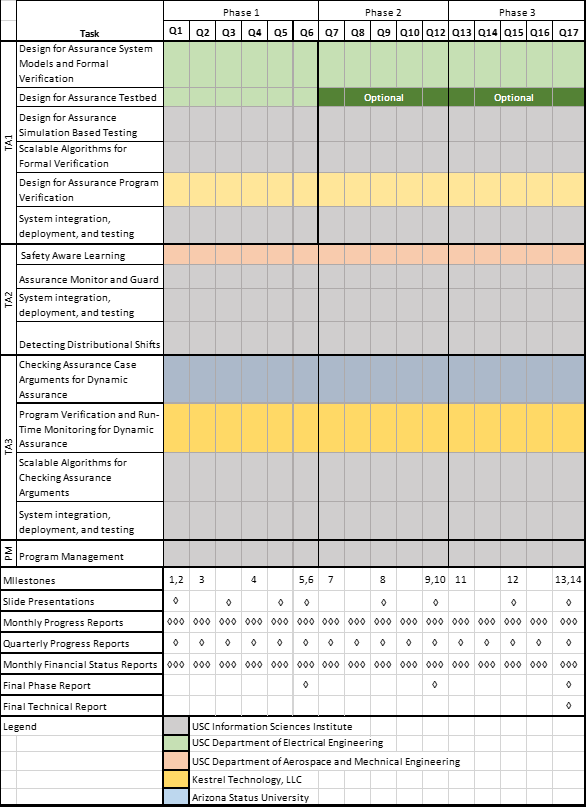
\includegraphics[width=.95\textwidth]{figs/Safeguard_Schedule_V6}
\end{center}
\vspace{-.2in}\caption{Project schedule along with a summary of milestones.  The legend maps task color to organization primary responsible for the task. } 
\label{fig:sandm}
\end{figure}
 

% \section{Level of Effort by Task \textcolor{red}{[Mike/Lisa - 1 pages]}}

% \textcolor{blue}{
% \begin{itemize}
% \item Will be a separate spreadsheet
% \item
% \end{itemize}
% }

\section*{Appendix A: Team Members and Other Information}
\addcontentsline{toc}{section}{Appendix A: Team Members and Other Information}

\baades{This section is mandatory and must include all of the following
components. If a particular subsection is not applicable, state “NONE”.}

\vspace{1ex}

\noindent
\textbf{Team Member Identification}:

\vspace{1ex}

\baades{Provide a list of all team members including the
prime, subcontractor(s), and consultant(s), as applicable. Identify specifically
whether any are a non-US organization or individual, FFRDC and/or Government
entity.}

\begin{centering}

%\small
\begin{tabular}{|p{1.8in}|p{1in}|p{1.1in}|p{0.7in}|p{0.8in}|p{0.7in}|}
\hline
 \textbf{Name} &  \textbf{Role} & \textbf{Organization} & \textbf{Non-US Org?}  & \textbf{Non-US Ind?} &  \textbf{FFRDC or Gov} \\
 \hline
Craig A. Knoblock & Prime & USC & N & N & N\\ \hline
Michael Orosz & Prime & USC & N &  N & N \\ \hline
Satish Thittamaranahalli & Prime & USC & N &  Y & N \\ \hline
Ryan Goodfellow & Prime & USC & N &  N & N \\ \hline
Anoop Kumar & Prime & USC & N & N & N \\ \hline
Satyandra Gupta & Prime & USC & N & N & N \\ \hline
Pierluigi Nuzzo & Prime & USC & N & Y & N \\ \hline
Petros Ioannou & Prime & USC & N & N & N \\ \hline
Chitta Baral & Subcontractor & ASU & N & N & N \\ \hline
Matt Barry & Subcontractor & Kestrel Technology & N & N & N \\ \hline
Douglas Smith & Subcontractor & Kestrel Technology & N & N & N \\ \hline
Henny Sipma & Subcontractor & Kestrel Technology & N & Y & N \\ \hline
\end{tabular} 
\end{centering}

\vspace{1ex}

\noindent
\textbf{Government or FFRDC Team Member Proof of Eligibility to Propose}: NONE

\baades {If
none of the team member organizations (prime or subcontractor) are a
Government entity or FFRDC, state “NONE”.}

\vspace{1ex}

\noindent
\textbf{Government or FFRDC Team Member Statement of Unique Capability}: NONE

\vspace{1ex}

\noindent
\textbf{Organizational Conflict of Interest Affirmations and Disclosure}: NONE

\vspace{1ex}

\noindent
\textbf{Intellectual Property (IP)}: 
\baades {
If no IP restrictions are intended, state “NONE”.
The Government will assume unlimited rights to all IP not explicitly identified as
having less than unlimited rights in the proposal.
For all technical data or computer software that will be furnished to the
Government with other than unlimited rights, provide (per Section VI.B.1) a list
describing all proprietary claims to results, prototypes, deliverables or systems
supporting and/or necessary for the use of the research, results, prototypes
and/or deliverables. Provide documentation proving ownership or possession of
appropriate licensing rights to all patented inventions (or inventions for which a
patent application has been filed) to be used for the proposed project.
}
\begin{centering}

%\small
\begin{tabular}{|p{2.1in}|p{1.2in}|p{1.4in}|p{2in}|}
\hline
\multicolumn{4}{|c|}{COMMERCIAL ITEMS }\\ \hline 
 \textbf{Technical Data, Computer Software To be Furnished With Restrictions} &  \textbf{Basis for Assertion} & \textbf{Asserted Rights Category} & \textbf{Name of Person Asserting Restrictions}  \\  \hline
KT Advance & Developed with mixed funding. & Restricted & David Kulich, Contracts Manager, Kestrel technology, LLC.\\ \hline
\end{tabular} 
\end{centering}

\vspace{1ex}

\noindent
\textbf{Human Subjects Research (HSR)}: NONE

\vspace{1ex}

\noindent
\textbf{Animal Use}: NONE

\vspace{1ex}

\noindent
\textbf{Representations Regarding Unpaid Delinquent Tax Liability or a Felony
Conviction under Any Federal Law}: 
%NONE

\begin{enumerate}
\item
The proposer is  not a corporation that has any unpaid Federal tax liability that has been assessed, for which all judicial and administrative remedies have been exhausted or have lapsed, and that is not being paid in a timely manner pursuant to an agreement with the authority responsible for collecting the tax liability,
\item
The proposer is not a corporation that was convicted of a felony criminal violation under a Federal law within the preceding 24 months.
\end{enumerate}

\vspace{1ex}

\noindent
\textbf{Cost Accounting Standards (CAS) Notices and Certification}:
\baades{
For any proposer who submits a proposal which, if accepted, will result in a CAS-compliant
contract, must include a Disclosure Statement as required by 48 CFR
9903.202. The disclosure forms may be found at
http://www.whitehouse.gov/omb/procurement\_casb
If this section is not applicable, state “NONE”. For further information regarding
this subject, please see www.darpa.mil/work-with-us/additional-baa.
}
NONE


%\section{Appendix B \textcolor{red}{[No Page Count]}}

\section{References}
\bibliographystyle{acm} 
\bibliography{TA3/ta3,TA2/ta2,TA1/ta1}
\end{document}
\clearpage
\newpage


\section{Management Plan}


The Principal Investigator for this effort is Dr. Craig Knoblock who is responsible for all aspects of the effort, will coordinate the parallel team efforts, and will ensure high levels of performance from individual team members.  The Co-P/I, Dr. Michael Orosz, will provide project management and will assist all performers in the execution of the project.    The project team is divided into three working groups (Figure~\ref{fig:org_chart}) corresponding to Technical Areas 1-3, however, members of each team contribute across all project activities.   Table~\ref{fig:Table_Mgmt} defines the major contributions of each project team member to the project tasks.

\begin{figure}[tbhp]
%\vspace{-25pt}
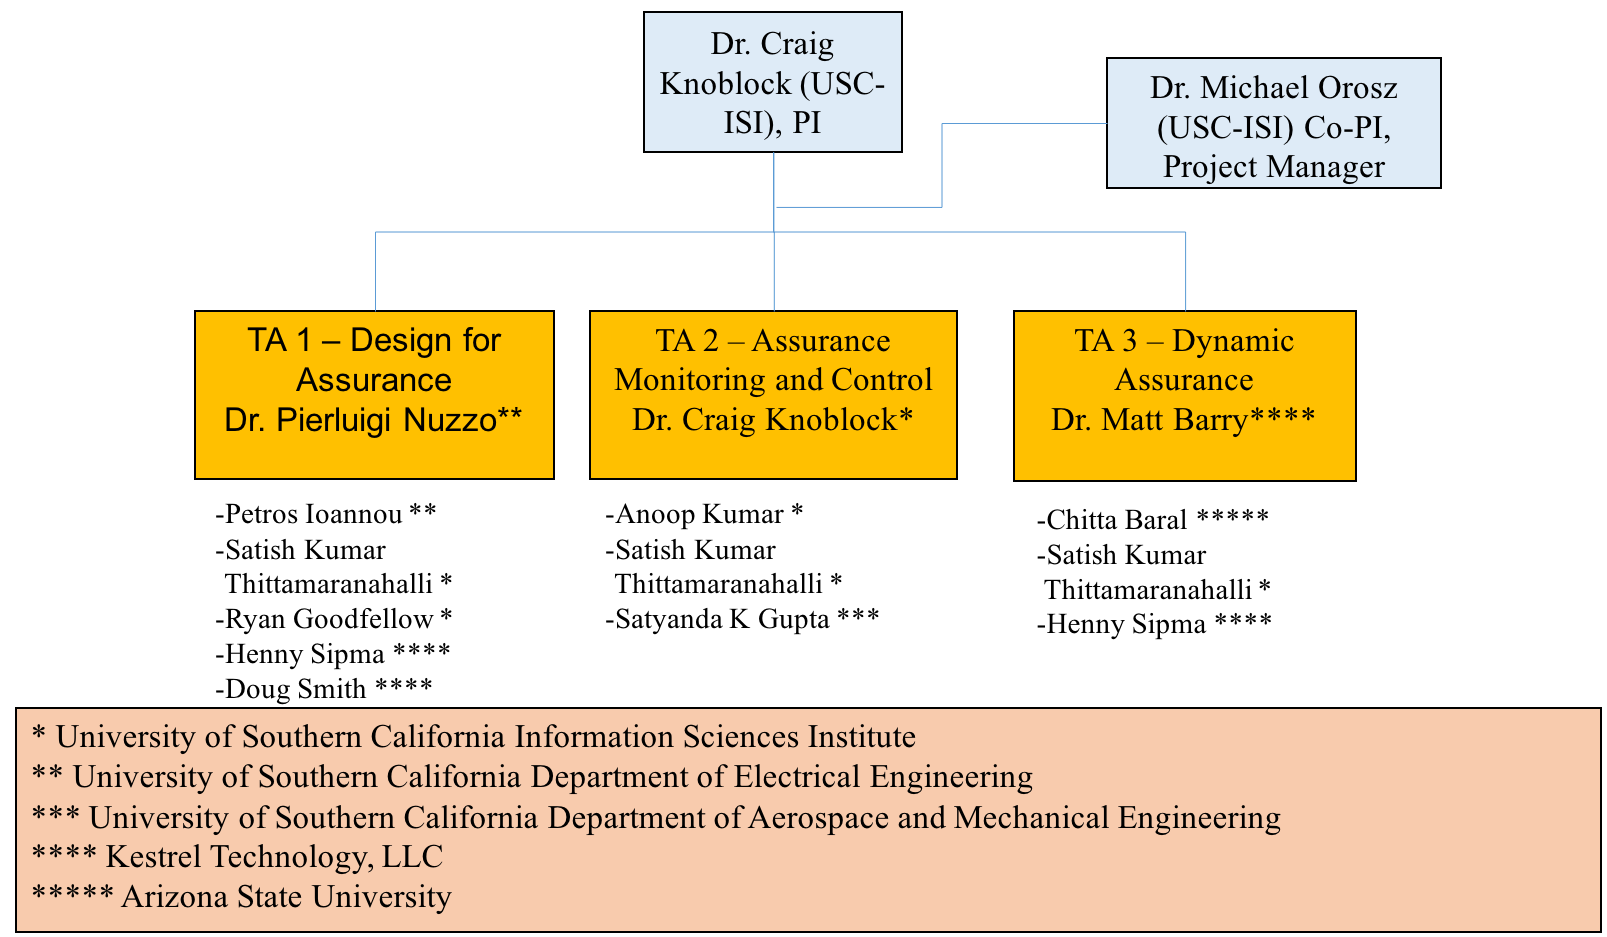
\includegraphics[width=6.0in]{./org-chart2.png}
\caption{\small Organization Chart}
\label{fig:org_chart}
\end{figure}

Coordination: To maximize collaboration and reduce risk to project failure from lack of communication and technical exchange, we plan to employ a wide variety of working styles and communication/coordination so that all can contribute.  At the core of our project will be regularly scheduled meetings bridging the diversely distributed team (Table~\ref{fig:Collaboration_Table}).  These meetings will address project status, identify challenges, implement risk mitigation strategies and participate in technology exchanges and system integration efforts (when appropriate)

\begin{table}[ht]
\caption{\small Project Meetings and Events}
  \centering
  {\footnotesize
\begin{tabular}{|m{3.15in}|m{3in}|} 
\hline
\textbf{Meeting} & \textbf{Frequency} 
\\\hline
Conference calls among investigators (discuss project status, address concerns and project risks) & Weekly
\\
\hline
Technical exchange and coordination meetings using Bluejeans or another videoconference technology & At least twice a month and more frequently as needed
  \\ 
\hline
Face-to-Face meetings (prior to P/I and demonstration meetings) & Every 3 to 6 months and more frequently (especially at the beginning of the project) as needed
 \\\cline{1-2}

\hline
\end{tabular}
}
\label{fig:Collaboration_Table}
\end{table}

\begin{table}[tbhp]
\caption{\small Key Project Team Member Responsibilities}
  \centering
  {\footnotesize
\begin{tabular}{| m{.75in} | m{3.9in}| m{1.5in}|} 
\hline
\textbf{Key Member} & \textbf{Responsibilities} & \textbf{Tasks} 
\\\hline
Dr.\ Craig Knoblock  & Principal Investigator responsible for project, leads TA 2 – Assurance Monitoring and Control.  Will lead the overall project and lead the TA2 team.  Served as the PI on many DARPA projects and has sucessfully led many large teams.    Effort on project:  25\% &
1.1.6, 1.2.2 1.2.3, 1.2.4, 1.3.4, 1.4.1, 
2.1.6, 2.2.2 2.2.3, 2.2.4, 2.3.4, 2.4.1, 
3.1.6, 3.2.2, 3.2.3, 3.2.4, 3.3.4, 3.4.1
\\
\hline
Dr.\ Michael Orosz & Co-Principal Investigator responsible managing the day-to-day operations of the project, assist technical teams as needed, coordinate with TA4 teams.    Has led many large complex multi-disciplined/multi-organizational projects in academic and industry environments.  Effort on project: 50\%
& 1.1.6, 2.1.6, 3.1.6, 1.4.1, 2.4.1, 3.4.1
  \\ 
\hline
Dr.\ Pierluigi Nuzzo 
& 
Co-Principal Investigator.  Leads the TA 1 - Design for Assurance team and conducts research on the formal methods for the design of the TA1 system.  Research experience on methodologies and tools for the design of cyber-physical systems; contracts, interfaces, and compositional methods for embedded system design; the application of automated formal methods and optimization theory to problems in embedded and cyber-physical systems.  Effort on project: 2 months/year (16.6\%)
& 
1.1.1, 2.1.1, 3.1.1 \\
\hline
Dr.\ Matthew Barry
& 
Key personnel.  Leads the TA 3 – Dynamic Assurance.   He will conduct the research on the dynamic assurance case language editors and parsers, the run-time system, and system integrations. Effort on project:  66\%
& 
1.3.2, 2.3.2, 3.3.2\\
\hline
Dr.\ Chitta Baral
& 
Key personnel responsible for learning assurance rules, supporting assurance rules with uncertainty and improving solver speed.  Expertise on ASP solvers, which will be used to reason about the assurance cases. Effort on project: 20\%
& 
1.3.1, 2.3.1, 3.3.1 \\
\hline
Dr.\ Doug Smith 
& 
Key personnel will support formal methods aspects of TA1, and lead the effort on abstract refinement. Expertise in field of automated correct-by-construction program generation.    Effort on project: 40\%
& 
1.1.5, 2.1.5, 3.1.5 \\
\hline
Dr.\ Henny Sipma
& 
Key personnel who will support the program verification tasks under TA1.  Will lead the effort on program verification.   Effort on project:  45\%
& 
1.1.5, 2.1.5, 3.1.5, 1.3.2, 2.3.2, 3.3.2 \\
\hline
Dr.\ Petros Ioannou
& 
Key personnel responsible providing and extending the assurance test bed, which will be available at the start of the project for autonomous vehicles.   Effort on project: 1 month/year (8.3\%)
& 
1.1.2, 2.1.2 (optional), 3.1.2 (optional)
\\
\hline
Dr.\ Satyandra Kumar Gupta
& 
Key Personnel providing autonomous command and control expertise to the TA-2 team.   Will lead the research on safety aware learning on TA2.   Past research on physics-aware decision making to facilitate automation.  Effort on project: 1 month/year (8.3\%)
& 
1.2.1, 2.2.1, 3.2.1 \\
\hline
Dr.\ Anoop Kumar 
& 
Key personnel providing support to the TA 2 project team.  Will lead the research on monitoring \& control and detecting distribution shifts.  Effort on project: 50\%
& 
1.2.1, 1.2.2, 1.2.3, 1.2.4, 2.2.1, 2.2.2, 2.2.3, 2.2.4, 3.2.1, 3.2.2, 3.2.3, 3.2.4\\
\hline
Dr.\ Satish Thittamaranahalli
& 
Key personnel developing scalable algorithms for TA1, TA2, and TA3 project teams.  Has extensive experience on scalable algorithm design, machine learning, and constraint reasoning.  Effort on project: 50\%
& 
1.2.1, 1.2.2, 1.2.3, 1.2.4, 2.2.1, 2.2.2, 2.2.3, 2.2.4, 3.2.1, 3.2.2, 3.2.3, 3.2.4, 1.1.4, 2.1.4, 3.1.4 \\
\hline
Dr.\ Ryan Goodfellow
& 
Key personnel providing support to the TA-1 project. Will lead the research on simulation-based testing.  Has extensive experience on simulation-based testing.  Effort on project:  30\%
& 
1.1.3, 2.1.3, 3.1.3 \\

\cline{1-2}

\hline
\end{tabular}
}
\label{fig:Table_Mgmt}
\end{table}



\newpage
\section{Personnel, Qualifications and Commitment}

{\bf Dr.\ Craig Knoblock}, the PI on this effort, is a Research Professor of both Computer Science and Spatial Sciences at the University of Southern California (USC) and Director of the Intelligent Systems Division at the USC Information Sciences Institute.   He received his Ph.D. from Carnegie Mellon University in computer science. 
%His research focuses on techniques for describing, acquiring, and exploiting the semantics of data.  
In previous projects he has worked on developing  scalable approaches to execution monitoring, accurate detection of sensor failures, and   automatic modeling and reconstruction of sensors.  He has published more than 300 journal articles, book chapters, and conference papers on these topics.  Dr. Knoblock is a Fellow of the Association for the Advancement of Artificial Intelligence (AAAI), a Distinguished Scientist of the Association of Computing Machinery (ACM), a Senior Member of IEEE, past President and Trustee of the International Joint Conference on Artificial Intelligence.
%and winner of the 2014 Robert S. Engelmore Award.  

{\bf Dr.\ Michael Orosz}, a Co-PI on this effort, is a Research Associate Professor of Civil and Environmental Engineering at the University of Southern California (USC) and Research Director of the Decision Systems Group at the USC Information Sciences Institute.  Dr. Orosz has over 30 years’ experience in commercial and government software development, basic and applied research, project management, academic research and has developed and deployed several commercially successful products.  His research interests are in machine learning and decision analytics as applied to intelligence analysis and autonomous command and control such as smart building controls.    Dr. Orosz has extensive experience in managing large complex multi-disciplined/multi-teamed research projects. %funded by DARPA, DHS, DoD, DoE, Industry, NASA, NRO, NSA and ONR.   
He received his Ph.D. in computer science from the University of California, Los Angeles.

{\bf Dr.\ Pierluigi Nuzzo}, a Co-PI on this project, is an Assistant Professor in the Department of Electrical Engineering at the University of Southern California. He received the Ph.D. in Electrical Engineering and Computer Sciences from the University of California at Berkeley. 
%in 2015, and the Laurea degree (MS) in electrical engineering (summa cum laude) from the University of Pisa, Italy, and the Sant'Anna School of Advanced Studies, Pisa, Italy.
%
%He has four years of research experience in analog and mixed signal circuit design as a researcher at IMEC, Leuven, Belgium, and over 10 years experience in design methodologies and tools for mixed-signal integrated circuits and cyber-physical systems, as a researcher at the University of Pisa, IMEC, UC Berkeley, and USC. 
His research interests
include: methodologies and tools for cyber-physical system and mixed-signal
system design; contracts, interfaces and compositional methods for embedded
system design; the application of formal methods and optimization theory to problems in embedded and cyber-physical systems and electronic design automation. 
%
Prof. Nuzzo received %First Place in the operational category and Best Overall
%Submission in the 2006 DAC/ISSCC Design Competition, 
a Marie Curie Fellowship
from the European Union in 2006, 
the University of California at Berkeley EECS
departmental fellowship in 2008, 
%the University of California at Berkeley Outstanding Graduate Student Instructor Award in 2013, 
the IBM Ph.D.
Fellowship in 2012 and 2014, 
%the Best Paper Award from the International Conference on Cyber-Physical Systems (ICCPS) in 2016, 
and the David J.~Sakrison Memorial Prize in 2016 for his doctoral research. 
%He is an author of 1 patent and over 60 publications.

{\bf Dr.\ Satyandra K. Gupta} is Smith International Professor in the Department of Aerospace and Mechanical Engineering at the University of Southern California. %Prior to joining the University of Southern California, he was a Professor in the Department of Mechanical Engineering and the Institute for Systems Research at the University of Maryland. He was the founding director of the Maryland Robotics Center and the Advanced Manufacturing Laboratory at the University of Maryland. 
He served as a program director for the National Robotics Initiative at the National Science Foundation from September 2012 to September 2014.  Dr. Gupta's interest is in the area of physics-aware decision making to facilitate automation. He has published more than 300 technical articles. He is a fellow of the American Society of Mechanical Engineers (ASME) and editor of ASME Journal of Computing and Information Science in Engineering. Dr. Gupta has received the Young Investigator Award from the Office of Naval Research in 2000, CAREER Award from the National Science Foundation in 2001, Presidential Early Career Award for Scientists and Engineers (PECASE) in 2001, Invention of the Year Award at the University of Maryland in 2007, Kos Ishii-Toshiba Award from ASME in 2011, and Excellence in Research Award from ASME in 2013.%, and Distinguished Alumnus Award from Indian Institute of Technology, Roorkee in 2014. %He has also received seven best paper awards at conferences.

{\bf Ryan Goodfellow} is a computer scientist at ISI working in combined cyber physical simulation and emulation platform development. His formal background is in simulation algorithms and modeling techniques using differential-algebraic equations (DAE). He has applied this knowledge in the CPS space by integrating DAE modeling languages and simulation engines with network testbeds to create comprehensive scientific experimentation platforms for cyber-physical systems. These experimentation platforms have been used in the power grid research space. %Ryan is a lead developer on the Deter network testbed, with a strong background in networked and distributed systems engineering. %He is also a combat veteran, serving as a non-commissioned officer and SIGINT team lead for a multi-functional intelligence team in Afghanistan.

{\bf Dr.\ Petros Ioannou} is a Professor in the Department of Electrical Engineering, Director of the Center for Advanced Transportation Technologies and Associate Director for Research for the DOT supported University Transportation Center at USC. He received his MS and PhD from the University of Illinois at Urbana Champaign in Mechanical and Electrical Engineering, respectively. His research interests are in robust adaptive control, vehicle dynamics and control, human factors and safety, automated vehicles, nonlinear systems and Intelligent transportation Systems.  He received the 2016 IEEE Transportation Technologies field award and the 2016 IEEE Control system society Transition to Practice Award. He is a Fellow of IEEE, IFAC and IET and author/coauthor of 8 books and over 400 papers.

{\bf Dr.\ Matthew Barry} will serve as lead for the TA3 tasks. %He will implement the dynamic assurance case language editors and parsers, the run-time system, and system integrations.  He will implement the assurance case arguments and the API for updating argument structure and content.  
Dr. Barry currently is CEO at Kestrel Technology LLC, and previously spent 20 years in NASA space mission operations at the Jet Propulsion Lab and Johnson Space Center.  At NASA Headquarters he led the introduction of dependability case requirements and plans for flight computing systems in upcoming manned space exploration missions, as well as the development of Agency-level software-related safety-critical control system requirements.  He recently served as a Principal Investigator on DHS/Cyber S\&T STAMP (Static Tool Analysis Modernization Program), DARPA CSFV (Crowd Sourced Formal Verification), three NASA Aeronautics R\&D projects, and the AFRL-sponsored Static Analysis of Numerical Algorithms project.  Dr. Barry earned BSME, MS, and PhD degrees in mechanical engineering, and an MBA degree, from Rice University.  

{\bf Dr.\ Henny Sipma} will support the program verification tasks under TA1.  %She is the key person behind the company's {\em KT Advance\/} and {\em KT Transferal\/} static analysis products, and the designer and programmer of the company's core {\em CodeHawk\/} abstract interpretation engine. 
Dr. Sipma currently is the CTO at Kestrel Technology LLC.  She has spent the past 10 years with Kestrel Technology as a static analysis expert; previously developed and taught static analysis techniques as senior research associate at Stanford University for eight years; and developed industrial process controls as an senior systems analyst at Shell.  She has been Principal Investigator or company lead on several recent R\&D projects for Federal agencies, including two projects under the IARPA STONESOUP (Securely Taking On New Executable Software of Uncertain Provenance) program; the DHS Cyber S\&T Gold Standard project; and the DARPA-sponsored STAC (Space-Time Analysis for Cybersecurity) and MUSE (Mining and Understanding Software Enclaves) programs.  Dr. Sipma earned 
%a BS degree in chemistry and an MS degree in chemical engineering at the University of Groningen in The Netherlands, and 
MS and PhD degrees in computer science from Stanford University.  

{\bf Dr.\ Douglas R.\ Smith} will support formal methods aspects of TA1, including the enforcement of safety properties and the generation of monitors.  He is President of Kestrel Technology LLC and Principal Scientist at Kestrel Institute.  He is a Fellow of the American Association of Artificial Intelligence (AAAI) and an ASE Fellow (Automated Software Engineering).  From 1986 to 2000, he taught an advanced graduate course on correct-by-construction software development at Stanford.  
%Dr. Smith has led the development of a series of software synthesis systems, including KIDS (Kestrel Interactive Development System), Specware, Designware, and Planware. 
%Applications domains have included a variety of complex high-performance planners and schedulers for the US Air Force.  He leads current projects on the generation of air mission plans and cyberoperations.  
Other recent projects focused on automated policy enforcement \cite{SmithD0703,SmithD08}, synthesis of secure network protocol codes, and the synthesis of high-performance constraint-solvers\cite{SmithD08c,SmithD13}.  Dr. Smith has over 30 years experience in the field of automated correct-by-construction program generation and has published over 100 papers. He has one patent.  He received the Ph.D. in Computer Science from Duke University% in 1979.  

{\bf Dr. Chitta Baral} is a Professor in the Department of Computer Science and Engineering at Arizona State University. He will support the TA3 efforts on Learning assurance rules, supporting assurance rules with uncertainty and improving solver speed. Dr. Baral has expertise in various aspects of autonomy and Artificial Intelligence. 
He wrote the first book on answer set programming (published by Cambridge University Press) the formal language behind our assurance rules. Some of his other works relevant to this proposal are: goal specification for autonomous systems, automatic construction of control rules for autonomous systems that satisfy given goals, combining machine learning with reasoning in various contexts, including image understanding. %He is the President of KR Inc. He is an associate editor of AIJ and has been an associate editor of JAIR.

{\bf Dr.\ Satish Kumar Thittamaranahalli (T. K. Satish Kumar)} leads the Collaboratory for Algorithmic Techniques and Artificial Intelligence (CATAI) at USC's Information Sciences Institute. He has published over 60 papers on numerous topics in Artificial Intelligence spanning such diverse areas as Constraint Reasoning, Planning and Scheduling, Probabilistic Reasoning, Robotics, Combinatorial Optimization, Approximation and Randomization, Heuristic Search, Model-Based Reasoning, Knowledge Representation and Spatio-Temporal Reasoning. %He %has served on the Program Committees of many international conferences in Artificial Intelligence
He and is a winner of the 2016 Best Robotics Paper Award and the 2005 Best Student Paper Award from the International Conference on Automated Planning and Scheduling. 
Dr. Kumar received his PhD in Computer Science from Stanford University. %In the past, he has also been a Visiting Student at the NASA Ames Research Center, a Postdoctoral Research Scholar at the University of California, Berkeley, a Research Scientist at the Institute for Human and Machine Cognition, a Visiting Assistant Professor at the University of West Florida, and a Senior Research and Development Scientist at Mission Critical Technologies.

\textbf{Dr.\ Anoop Kumar} is a senior computer scientist at USC ISI and has broad expertise in machine learning, statistical modeling, and software engineering.  Dr.\ Kumar is the technical lead on the DARPA RSPACE program and has played a vital role in developing a system that fuses air operations data from multiple sources, maintains world state, and issues warnings. Previously, he led the research and development of the BBN’s election forecasting system for the IARPA OSI program. %Dr.\ Kumar played a significant role in the DARPA DEFT program by developing a model to support integration of output from multiple NLP algorithms. He has contributed at the development to management levels on government research contracts and commercial projects. 
Dr.\ Kumar helped design and develop BBN's commercially available, hosted speech and medical transcription services offering. 

\begin{table}[!tbh]
\begin{footnotesize}
\vspace{-0.1in}

\begin{tabular}{lll}
\begin{tabular}[t]{|l|@{}c@{}|@{}c@{}|@{}c@{}|@{}c@{}|} \hline
Project & Status & \multicolumn{3}{ c| }{Hours} \\ \cline{3-5}
& & P1 & P2 & P3 \\ \hline



\multicolumn{5}{ |c| }{ \textbf{Craig Knoblock} } \\ \cline{1-5}
Safeguard & Pro & 770 & 641 & 641 \\ \cline{1-5}
ELICIT & Cur & 308 & 256 & 120 \\ \cline{1-5}
WTNIC & Cur & 11 & 0 & 0 \\ \cline{1-5}
EFFECT & Cur & 641 & 107 & 0 \\ \cline{1-5}
LinkedMaps & Cur & 203 & 25 & 0 \\ \cline{1-5}
PRINCESS & Cur & 608 & 96 & 0 \\ \cline{1-5}
SCHARP & Cur & 481 & 54 & 0 \\ \cline{1-5}
MINT & Pen & 650 & 534 & 285 \\ \cline{1-5}

\multicolumn{5}{ |c| }{ \textbf{Michael Orosz} } \\ \cline{1-5}
Safeguard & Pro & 1560 & 1300 & 1300  \\ \cline{1-5}
SMC/SY & Cur & 1803 & 0 & 0  \\ \cline{1-5}

\multicolumn{5}{ |c| }{ \textbf{Matthew Barry} } \\ \cline{1-5}
Safeguard & Pro & 2078 & 1690 & 1554 \\ \cline{1-5}
Starlite & Cur & 1840 & 1692 & 0 \\ \cline{1-5}



\multicolumn{5}{ |c| }{ \textbf{Anoop Kumar} } \\ \cline{1-5}
Safeguard & Pro & 1560 & 1300 & 1300 \\ \cline{1-5}

\end{tabular}
&
\begin{tabular}[t]{|l|@{}c@{}|@{}c@{}|@{}c@{}|@{}c@{}|} \hline
Project & Status & \multicolumn{3}{ c| }{Hours} \\ \cline{3-5}
& & P1 & P2 & P3 \\ \hline

\multicolumn{5}{ |c| }{ \textbf{Pierluigi Nuzzo} } \\ \cline{1-5}
Safeguard & Pro & 520 & 433 & 433  \\ \cline{1-5}
Mirage & Cur & 433 & 0 & 0  \\ \cline{1-5}

\multicolumn{5}{ |c| }{ \textbf{Satyandra Gupta} } \\ \cline{1-5}
Safeguard & Pro & 260 & 217 & 217 \\ \cline{1-5}
Human   & Cur & 22 & 0 & 0 \\ \cline{1-5}
Vehicles & Cur & 36 & 0 & 0 \\ \cline{1-5}
Robot & Cur & 116 & 0 & 0 \\ \cline{1-5}
Assembly & Cur & 33 & 0 & 0 \\ \cline{1-5}
Solar & Cur & 4 & 0 & 0 \\ \cline{1-5}

\multicolumn{5}{ |c| }{ \textbf{Petros Ioannou} } \\ \cline{1-5}
Safeguard & Pro & 260 & 217 & 217 \\ \cline{1-5}
CPS & Cur & 130 & 0 & 0 \\ \cline{1-5}

\multicolumn{5}{ |c| }{ \textbf{Ryan Goodfellow} } \\ \cline{1-5}
Safeguard & Pro & 936 & 780 & 780 \\ \cline{1-5}
STEAM & Cur & 416 & 0 & 0 \\ \cline{1-5}


\end{tabular}
&
\begin{tabular}[t]{|l|@{}c@{}|@{}c@{}|@{}c@{}|@{}c@{}|} \hline
Project & Status & \multicolumn{3}{ c| }{Hours} \\ \cline{3-5}
& & P1 & P2 & P3 \\ \hline

\multicolumn{5}{ |c| }{ \textbf{Chitta Baral} } \\ \cline{1-5}
Safeguard & Pro & 659 & 485 & 485 \\ \cline{1-5}
PostdocBP & Cur & 176 & 0 & 0 \\ \cline{1-5}
Languages & Pen & 528 & 264 & 264 \\ \cline{1-5}
CAREER & Pen & 88 & 44 & 44 \\ \cline{1-5}
CHS & Pen & 510 & 255 & 0 \\ \cline{1-5}

\multicolumn{5}{ |c| }{ \textbf{Doug Smith} } \\ \cline{1-5}
Safeguard & Pro & 1222 & 984 & 840 \\ \cline{1-5}
RSPACE & Cur & 342 & 0 & 0 \\ 
\cline{1-5}
PLANX & Cur & 154 & 0 & 0 \\ 
\cline{1-5}
HACCS & Pen & 923 & 769 & 769 \\ 
\cline{1-5}

\multicolumn{5}{ |c| }{ \textbf{Henny Sipma} } \\ \cline{1-5}
Safeguard & Pro & 1372 & 962 & 840 \\ \cline{1-5}
STAC & Cur & 797 & 0 & 0 \\ \cline{1-5}

\multicolumn{5}{ |c| }{ \textbf{Satish Thittamaranahalli} } \\ \cline{1-5}
Safeguard & Pro & 1560 & 1300 & 1300 \\ \cline{1-5}
MapF & Cur & 103 & 103 & 0 \\ \cline{1-5}

\end{tabular}
\end{tabular}

\end{footnotesize}
\caption{Individual commitments of key personnel}
\label{tab:Commitments}
\vspace{-0.2in}
\end{table}

\clearpage
\newpage
\section{Capabilities}


%\subsection{University of Southern California}
USC has strengths in number of areas that are closely related to the proposed work:
\begin{itemize}[itemsep=0pt,leftmargin=*]
\item Dr.\ Nuzzo 
%has over 10-year research experience in embedded system design, from mixed-signal chip design (analog-to-digital converters, frequency synthesizers, software-defined radio), to methodologies and tools for mixed-signal integrated circuits and Cyber-Physical Systems (CPSs), and the application of formal methods and optimization theory to problems in embedded and cyber-physical systems and electronic design automation.  
%His doctoral work 
has done extensive research on contracts and compositional methods for heterogeneous system design and design space exploration, with application to aircraft electric power systems and environmental control systems. His work has helped transition rigorous system design foundations, innovative design methodologies, and new systems engineering paradigms to industry (IBM, United Technologies). 
\item Dr.\ Satyandra K. Gupta has worked on autonomous surface vehicles, autonomous ground vehicles for operation on rugged terrains, and autonomous flapping wing aerial vehicles.   His group has developed a hierarchal decision making approach for realizing autonomous systems. 
%This approach combines task planning and assignment, deliberative trajectory planning, reactive collision avoidance behaviors, and trajectory tracking control layers. 
His group has also developed new methods for learning reactive behaviors in adversarial environments and COLREGS compliant trajectory planning. \item Dr.\ Knoblock has developed methods that learn the relationships between sensors to both identify failures and changes in sensor and reconstruct those sensors, providing estimates of the accuracy of the reconstructed sensors.  
\item Ryan Goodfellow has extensive experience in simulation based testing through high-fidelity CPS testbed environment development and operation, using the Deter network testbed as the core which has supported several large scale government projects from a variety of agencies and thousands of users. %we have developed sophisticated CPS experiments under programs such as NFS RIPS, NIST SmartCities and the DHS Cybersecurity showcase.
\item Dr.\ Ioannou %helped  design and implement adaptive cruise control systems in collaboration with Ford Motor Company, which was commercialized four years before any other company. He 
worked on several DOT funded projects on automated vehicles and intelligent highway systems where he demonstrated his vehicle control designs for safety and performance on actual automated vehicles in test trucks and I-15 highway.
\item Drs.\ Knoblock, Kumar, and Thittamaranahalli have developed highly scalable approaches for monitoring message traffic to identify potential problems and issue warnings and alerts. 
\item Dr. Thittamaranahalli has developed state-of-the-art methods for efficiently solving large-scale search and optimization problems. %These techniques will be applicable in TA2 for safety-aware learning and planning, in TA2 for assurance monitoring and control, and in TA3 for dynamic assessment of assurance cases.

\end{itemize}
%\subsection{Kestrel Technology LLC}

Kestrel Technology's strength is in program analysis, specifically static analysis of both source and binary targets.  The company performs applied R\&D and product development for a variety of static analysis applications  pivoting primarily on the abstract interpretation technique.  The company recently initiated development of program analysis applications using logical equivalence techniques. As a provider of verification evidence in the form of mathematical proofs, the company also has expertise in the design and development of assurance case arguments for high-integrity systems using such evidence. %The company is engaged in a partnership with Wind River Systems to develop program analysis tools for its embedded system developers.  Many of Wind River's customers must develop their products under safety and certification standards, including those using safety cases.  

   

%\subsection{Arizona State University}
Chitta Baral at Arizona State University has developed various software to learn assurance rules and various ASP solvers, which he has made available as open-source.

Most of the software carried forward for implementation or derivation is open source.  The single exception is Kestrel Technology's {\it KT Advance\/} static analysis tool (TA1), in particular the abstract interpretation engine therein, which is company proprietary and is US EAR export-controlled.   
%Owing to mixed funding for the development of that technology 
We will continue to provide the Federal government a restricted use license for that particular item.

There are no specialized facilities, data, or GFE required for this effort. 


\section{Statement of Work}
We propose work for TA 1 – TA 3 for all three phases. All tasks span the four years of the program. For each task we provide an objective, the high-level approach (focusing on the responsibilities of each contributing organization), and the specific approach and milestones planned for each task for each phase. On all tasks, we will deliver design documents, software implementations, demonstrations, and publications. With the exception of several tasks accomplished by Kesler Technology, LLC, all tasks that accomplished at a university (USC/ISI, USC, and ASU) are believed to be fundamental research.   
%\usepackage[table]{xcolor}

{\scriptsize

\begin{longtable} {|p{\textwidth} | }

\hline

\textcolor{blue} {\footnotesize {\textbf{Tasks 1.1.1, 2.1.1, 3.1.1 -Design for Assurance System Models and Formal Verification (USC)}}} \\ \hline
Objective:  Develop contract-based formalisms and mapping tools to represent and reason about LE-CPSs at multiple levels of abstraction and generate assurance cases.  Undertake scalable formal verification and synthesis via Satisfiability Modulo Convex Programming. \\ \hline
Approach:  Develop modeling formalisms to represent components and contracts for LE-CPSs, including physical plant (e.g., autonomous vehicle, sensors, actuators, environment, controllers, and learning components. Formalisms will encompass different control and learning architectures (e.g., neural networks, statistical methods, graphical models, ensemble methods, decision trees) and support mapping between abstractions.   Develop a formal domain-specific language to capture and formalize requirements on LE components, systems, and their dynamics as contracts.   Develop a unifying framework and efficient algorithms to reason about the combination of discrete and continuous dynamics and constraints in the presence of uncertainties in LE cyber-physical systems \\ \hline
Phase 1 (1.1.1):  Milestone 1: Develop initial design followed by development and testing of individual components.  Milestone 2:  Library of components and contracts for the autonomous vehicle application driver.  Milestone 4: Library of components and contracts for the platforms provided by TA4 performers. Extension of the methodology and to support up to 20 continuous dimensions and 2 learning components for the 2 application drivers from TA4.  Milestone 6: -Prototype toolkit (software package) for capturing requirements, for translating them into contracts, for analyzing and validating them using contract operations and relations.  Prototype toolkit for capturing probabilistic requirements and behaviors of LE components, systems, and their dynamics, for translating them into stochastic assume-guarantee contracts, for analyzing and validating them using contract operations and relations, and for synthesizing design and verification artifacts from contracts.  Extension of the SMC framework and toolkit to support reactive and robust task and trajectory planning in the presence of uncertainties. \\ \hline
Phase 2 (2.1.1) Milestone 7: Refinement of design.  Milestone 9: extension of methodology, design, toolkits and libraries to support 40 continuous dimensions, 4 LECs, 30\% monitoring overhead. Extension of the SMC framework and toolkit from Phase 1 to support verification and synthesis on system with 40 dimensions and 4 LECs.  Milestone 10: Demonstration of the SMC framework and toolkit.  Contribution to Phase II report and dissemination of the results in conferences and journals. \\ \hline
Phase 3 (3.1.1) Milestone 11: Update design based on Phase II demo.  Milestones 12-13:  extend methodology, design, toolkits and libraries to support 100 dimensions, 6 LECs and 10\% monitoring overhead.   Milestone 14: Undertake Phase III demonstration on both platforms and submit final project report. \\ \hline
\textcolor{blue} {\footnotesize {\textbf{Tasks 1.1.2, 2.1.2, 3.1.2: Design for Assurance Testbed (USC)} }}\\ \hline
Objective:  Develop a simulation test bed for data generation and LE algorithm testing, redesign and/or refinement.   Simulator used as the test bed until the TA4 platforms are available.   Test bed will be used for internal research/prototype after TA4 platform availability. \\ \hline
Approach:  Leverage previous work on microscopic traffic simulations in urban and rural environments using the commercial software VISSIM and Vortex Studio and built in extensions for automated driving.   Develop testbed for autonomous vehicles in road/off-road environments to allow LEs to collect data, learn and make control decisions on line and in real time by simulating scenarios. The testbed together with analytical tools used to refine and redesign LEs and control algorithms by taking into account effects revealed by the simulation and not accounted for in the design stage.    In the event the TA4 platforms are not available, the test bed will be extended further by integrating all the LE components, controllers and sensors for demonstration purposes and evaluation of the proposed methodology. \\ \hline
Phase 1 (1.1.2):  Milestones 1-2:  Extension of existing simulator test beds.  Milestones 3-5:  Testing of individual components under normal and unpredicatble situations and demonstrating the results in VISSIM under several different driving scenarios. \\ \hline
Phase 2 (2.1.2) – Optional:  Milestones 7-8:  Extension of existing simulator test beds to support the TA1-TA3 teams.  Milestones 9-10:  Support demonstration of technology capable of supporting 40 dimensions, 4 LECs and 30\% monitoring overhead. \\ \hline
Phase 3 (3.1.2) – Optional:  Milestones 11-12:  Extension of existing simulator test beds to support the TA1-TA3 teams.  Milestones 13-14:  Support demonstration of technology capable of supporting 100 dimensions, 6 LECs and 10\% monitoring overhead. \\ \hline
\textcolor{blue} {\footnotesize {\textbf{Tasks 1.1.3, 2.1.3, 3.1.3: Design for Assurance Simulation Based Testing (USC/ISI)}}} \\ \hline
Objective:  Develop external Discrete Control Mechanisms for OpenModelica.  Develop/package virtual-machine based static time dilation systems. Undertake network testbed integration and develop physical system behavioral analysis tooling. \\ \hline
Approach:  Leverage previous external discrete control mechanisms for DAEs, implement similar facilities for OpenModelica to allow LEs to observe and control a physical system over a network. Contributions pushed back upstream to OpenModelica project.  Implement DieCast for modern libvirt.  Develop tooling to deploy integrated CPS models on the Deter network testbed. Apply modern DAE control theory in the form Modelica analysis packages usable by non DAE experts. \\ \hline
Phase 1 (1.1.3):  Milestones 1-2:  Initial CPS simulation concept and components.  Milestones 3-5:  Testing of individual components under normal and unpredictable situations and demonstrating the results capable of meeting 20 dimensions, 2 LECs and 50\% or under monitoring overhead conditions.   Milestone 6: Demonstrate technology in Phase I demonstration, contribute to Phase I final report and disseminate software and publications. \\ \hline
Phase 2 (2.1.3):  Milestones 7-8:  Apply lessons learned from Phase I and extend existing simulations to support 30 dimensions, 3 LECs and 40\% monitoring overhead.  Milestones 9-10:  Support demonstration of technology capable of supporting 40 dimensions, 4 LECs and 30\% monitoring overhead.  Contribute to Phase II final report and disseminate software and publications. \\ \hline
Phase 3 (3.1.3):  Milestones 11-12:  Apply lessons learned from Phase II and extend existing simulations to support 70 dimensions, 5 LECs and 20\% monitoring overhead.  Milestones 13-14:  Support demonstration of technology capable of supporting 100 dimensions, 6 LECs and 10\% monitoring overhead.  Contribute to Phase III final report and disseminate software and publications. \\ \hline
\textcolor{blue} {\footnotesize {\textbf{Tasks 1.1.4, 2.1.4, 3.1.4: Scalable Algorithms for Formal Verification (USC/ISI)}}} \\ \hline
Objective: Develop innovative algorithms for scalable formal verification. \\ \hline
Approach: Use state-of-the-art techniques for solving combinatorial problems with discrete/continuous variables and hybrid constraints. \\ \hline
Phase 1 (Task 1.1.4): Milestones 1-2: Develop initial design plan and initial concepts. Milestones 3-5: Integrate framework that is capable of supporting 20 dimensions, 2 LECs and 0.1x trials to assurance. Milestone 6: Participate in Phase I demonstration, contribute to Phase I final report and disseminate software and publications. \\ \hline
Phase 2 (Task 2.1.4): Milestones 7-8: Apply lessons learned from Phase I and extend existing design to support 30 dimensions, 3 LECs and 0.05x trials to assurance. Milestones 9-10: Demonstrate technology capable of supporting 40 dimensions, 4 LECs and 0.01x trials to assurance. Participate in Phase II demonstration, contribute to Phase II final report and disseminate software and publications. \\ \hline
Phase 3 (Task 3.1.4): Milestones 11-12: Apply lessons learned from Phase II and extend design/approach to support 70 dimensions, 5 LECs and 0.005x trials to assurance. Milestones 13-14: Demonstrate technology capable of supporting 100 dimensions, 6 LECs and 0.001x trials to assurance. Complete integration of technology into TA4 platform. Contribute to Phase III final report and disseminate software and publications. \\ \hline
\textcolor{blue} {\footnotesize {\textbf{Tasks 1.1.5, 2.1.5, 3.1.5: Design for Assurance Program Verification (Kestrel Technology, LLC)}}} \\ \hline
Objective: Develop and integrate program analysis and monitor synthesis functionality with TA1 functions and services and integrate combined TA1 functions with TA4 platform. \\ \hline
Approach: Integrate existing analysis tools into development environment.  Design and implement abstract domains and properties for one or more modeling layers.  Design and implement analyzer front-end for modeling layers.  Implement test framework for verification tools.  Implement content providers and/or consumers for DAC via DAC API.  Leverage existing algorithms and tools to generate monitors for assumptions and unproven safety constraints. Integrate program analysis and monitor synthesis functionality with TA1 functions and services, integrate combined TA1 functions with TA4 platform.   Prepare software and data installation kits and operating instructions;install software and confirm configuration. \\ \hline
Phase 1 (1.1.5) : Milestones 1-2:  Initial framework design and unit tools, TA1-TA3 interfaces defined. Milestones 3-5:  Testing of individual components/tools capable of meeting 20 dimensions, 2 LECs and 50\% or under monitoring overhead conditions.   Milestone 6: Demonstrate technology in Phase I demonstration, contribute to Phase I final report and disseminate software and publications. \\ \hline
Phase 2 (2.1.5): Milestones 7-8:  Apply lessons learned from Phase I and extend existing design to support 30 dimensions, 3 LECs and 40\% monitoring overhead.  Milestones 9-10:  Support demonstration of technology capable of supporting 40 dimensions, 4 LECs and 30\% monitoring overhead.  Contribute to Phase II final report and disseminate software and publications. \\ \hline
Phase 3 (3.1.5): Milestones 11-12:  Apply lessons learned from Phase II and extend existing simulations to support 70 dimensions, 5 LECs and 20\% monitoring overhead.  Milestones 13-14:  Support demonstration of technology capable of supporting 100 dimensions, 6 LECs and 10\% monitoring overhead.  Contribute to Phase III final report and disseminate software and publications. \\ \hline
\textcolor{blue} {\footnotesize {\textbf{Tasks 1.1.6, 2.1.6, 3.1.6: System integration, deployment, and testing (USC/ISI)}}} \\ \hline
Objective: Develop and implement integration, testing and deployment plan supporting TA1 for all three phases. \\ \hline
Approach: Develop an internal TA1 integration and testing plan (unit tests, etc.) and, in close collaboration with TA2 and TA3 performers on project, develop an overall TA1-TA3 integration and testing plan.  Working with TA4 performers, extend and execute plan for TA4 platform (when available). \\ \hline
Phase 1 (1.1.6): Milestones 1-2:  Develop initial integration and testing plan and implement on unit testing.  Milestones 3-5:  Oversee integration and testing of TA1-TA3 components for system capable of supporting 20 dimensions, 2 LECs and 50\% or less monitoring overhead.   Milestone 6: Complete integration of technology into TA4 testbeds, contribute to Phase I final report and disseminate software and publications. \\ \hline
Phase 2 (2.1.6): Milestones 7-8:  Apply lessons learned from Phase I and extend existing integration and testing plan to support 30 dimensions, 3 LECs and 40\% monitoring overhead.  Milestones 9-10:  Support demonstration of technology capable of supporting 40 dimensions, 4 LECs and 30\% monitoring overhead.  Complete integration of technology into TA4 platforms.  Contribute to Phase II final report and disseminate software and publications. \\ \hline
Phase 3 (3.1.6): Milestones 11-12:  Apply lessons learned from Phase II and extend existing integration and testing plan to support 70 dimensions, 5 LECs and 20\% monitoring overhead.  Milestones 13-14:  Support demonstration of technology capable of supporting 100 dimensions, 6 LECs and 10\% monitoring overhead.  Complete integration of technology into TA4 platform.  Contribute to Phase III final report and disseminate software and publications. \\ \hline
\textcolor{blue} {\footnotesize {\textbf{Tasks 1.2.1, 2.2.1, 3.2.1: Safety Aware Learning (USC)} }}\\ \hline
Objective: Enable the system to learn efficiently without violating safety constraints. \\ \hline
Approach: Integrate LECs with search methods to select the optimal actions/maneuvers to maximize mission utility. \\ \hline
Phase 1 (Task 1.2.1): Milestones 1-2:  Develop initial design plan and initial concepts. Milestones 3-5:  Integrate two LECs with search methods and integrate into framework that is capable of supporting 20 dimensions, 2 LECs and 50\% or less monitoring overhead.   Milestone 6: Participate in Phase I demonstration, contribute to Phase I final report and disseminate software and publications. \\ \hline
Phase 2 (Task 2.2.1): Milestones 7-8:  Apply lessons learned from Phase I and extend existing design to support 30 dimensions, 3 LECs and 40\% monitoring overhead.  Milestones 9-10:  Support demonstration of technology capable of supporting 40 dimensions, 4 LECs and 30\% monitoring overhead.  Participate in Phase II demonstration.  Contribute to Phase II final report and disseminate software and publications. \\ \hline
Phase 3 (Task 3.2.1): Milestones 11-12:  Apply lessons learned from Phase II and extend design/approach to support 70 dimensions, 5 LECs and 20\% monitoring overhead.  Milestones 13-14:  Support demonstration of technology capable of supporting 100 dimensions, 6 LECs and 10\% monitoring overhead. Complete integration of technology into TA4 platform.  Contribute to Phase III final report and disseminate software and publications. \\ \hline
\textcolor{blue} {\footnotesize {\textbf{Tasks 1.2.2, 2.2.2, 3.2.2: Assurance Monitor and Guards (USC)}}} \\ \hline
Objective: Build scalable algorithms for assurance monitoring of architectural and safety constraints \\ \hline
Approach: Use physical models to reduce processing of sensor information for assurance monitoring. Use Variable Elimination to handle uncontrollable, Adversarially controlled, or unobservable variables \\ \hline
Phase 1 (Task 1.2.2): Milestones 1-2:  Develop initial design plan and initial concepts.  Milestones 3-5:  Develop monitors for two LECs and integrate into framework that is capable of supporting 20 dimensions, 2 LECs and 50\% or less monitoring overhead.  Develop APIs for integration with TA1 and TA3. Milestone 6: Participate in Phase I demonstration, contribute to Phase I final report and disseminate software and publications. \\ \hline
Phase 2 (Task 2.2.2): Milestones 7-8:  Apply lessons learned from Phase I, incorporate physical models of vehicle-environment interactions and extend existing design to support 30 dimensions, 3 LECs and incorporate physical models to bring down monitoring overhead to 40\% or less.   Milestones 9-10:  Support demonstration of technology capable of supporting 40 dimensions, 4 LECs and 30\% monitoring overhead.  Participate in Phase II demonstration.  Contribute to Phase II final report and disseminate software and publications. \\ \hline
Phase 3 (Task 3.2.2): Milestones 11-12:  Apply lessons learned from Phase II and identify core constraints to monitor and correlation between variables to support 70 dimensions, 5 LECs and 20\% monitoring overhead.  Milestones 13-14:  Support demonstration of technology capable of supporting 100 dimensions, 6 LECs and 10\% monitoring overhead.  Complete integration of technology into TA4 platform.  Contribute to Phase III final report and disseminate software and publications. \\ \hline
\textcolor{blue} {\footnotesize {\textbf{Tasks 1.2.3, 2.2.3, 3.2.3: System integration, deployment, and testing: (USC/ISI)}}} \\ \hline
Objective: Develop and implement integration, testing and deployment plan supporting TA2 for all three phases. \\ \hline
Approach: Develop an internal TA2 integration and testing plan (unit tests, etc.) and, in close collaboration with TA1 and TA3 performers on project, develop an overall TA1-TA3 integration and testing plan.  Working with TA4 performers, extend and execute plan for TA4 platform (when available). \\ \hline
Phase 1 (1.2.3): Milestones 1-2:  Develop initial integration and testing plan and implement on unit testing.  Milestones 3-5:  Oversee integration and testing of TA1-TA3 components for system capable of supporting 20 dimensions, 2 LECs and 50\% or less monitoring overhead.   Milestone 6: Complete integration of technology into TA4 testbeds, contribute to Phase II final report and disseminate software and publications. \\ \hline
Phase 2 (2.2.3): Milestones 7-8:  Apply lessons learned from Phase II and extend existing integration and testing plan to support 30 dimensions, 3 LECs and 40\% monitoring overhead.  Milestones 9-10:  Support demonstration of technology capable of supporting 40 dimensions, 4 LECs and 30\% monitoring overhead.  Complete integration of technology into TA4 platforms.  Contribute to Phase II final report and disseminate software and publications. \\ \hline
Phase 3 (3.2.3): Milestones 11-12:  Apply lessons learned from Phase II and extend existing integration and testing plan to support 70 dimensions, 5 LECs and 20\% monitoring overhead.  Milestones 13-14:  Support demonstration of technology capable of supporting 100 dimensions, 6 LECs and 10\% monitoring overhead.  Complete integration of technology into TA4 platform.  Contribute to Phase III final report and disseminate software and publications. \\ \hline
\textcolor{blue} {\footnotesize {\textbf{Tasks 1.2.4, 2.2.4, 3.2.4: Detecting Distributional Shifts (USC)}}} \\ \hline
Objective:  Develop a comprehensive framework to detect distribution shifts in LECs \\ \hline
Approach: Extend our prior work on sensor failure detection to distribution shifts.  Implement an approach that looks at single variable, sliding window, and distributions and employs classifiers and ensemble methods. \\ \hline
Phase 1 (Task 1.2.4): Milestones 1-2:  Develop initial design plan and initial concepts.  Milestones 3-5:   Develop framework that is capable of supporting 20 dimensions, 2 LECs and 50\% or less monitoring overhead. Extend sensor failure detection in BRASS effort to detect distributional shifts.  Milestone 6: Participate in Phase I demonstration, contribute to Phase I final report and disseminate software and publications. \\ \hline
Phase 2 (Task 2.2.1): Milestones 7-8:  Apply lessons learned from Phase I and  implement sliding window and sampling based methods to support 30 dimensions, 3 LECs and 40\% monitoring overhead.  Milestones 9-10:  Support demonstration of technology capable of supporting 40 dimensions, 4 LECs and 30\% monitoring overhead.  Participate in Phase II demonstration.  Contribute to Phase II final report and disseminate software and publications. \\ \hline
Phase 3 (Task 3.2.1): Milestones 11-12:  Apply lessons learned from Phase II and implement data reduction and machine learning techniques to support 70 dimensions, 5 LECs and 20\% monitoring overhead.  Milestones 13-14:  Support demonstration of technology capable of supporting 100 dimensions, 6 LECs and 10\% monitoring overhead.  Complete integration of technology into TA4 platform.  Contribute to Phase III final report and disseminate software and publications. \\ \hline
\textcolor{blue} {\footnotesize {\textbf{Tasks 1.3.1, 2.3.1, 3.3.1 - Checking Assurance Case Arguments for Dynamic Assurance – (ASU)}} }\\ \hline
Objective: Enhance assurance case DSL to accommodate learning of assurance rules.    Enhance Dynamic Assurance Case (DAC) implementation to support uncertainty.   Enable ASP solver speed improvements 
 \\ \hline
Approach: We will develop algorithms and an implemented module that can learn assurance rules from a set of input-output pairs. We will illustrate the scalability of our method as compared to existing Inductive Logic Programming methods.  We will develop a variant of L that incorporates various uncertainty and automated reasoning related features such as causality, counterfactual reasoning, use of weights for computing probabilities and probabilistic non-monotonicity.  We will develop a highly efficient ASP reasoning system (that forms the heart of our assurance case DSL) by modularizing the ASP programs and making domain specific restrictions (such as stratification on a big part of the program) on the modules \\ \hline
Phase 1 (Task 1.3.1): Milestones 1-2:  Develop initial design plan and initial concepts.  Milestones 3-5:  Integrate two LECs with search methods and integrate into framework that is capable of supporting 20 dimensions, 2 LECs and 50\% or less monitoring overhead.   Milestone 6: Participate in Phase I demonstration, contribute to Phase I final report and disseminate software and publications. \\ \hline
Phase 2 (Task 2.3.1): Milestones 7-8:  Apply lessons learned from Phase I and extend existing design to support 30 dimensions, 3 LECs and 40\% monitoring overhead.  Milestones 9-10:  Support demonstration of technology capable of supporting 40 dimensions, 4 LECs and 30\% monitoring overhead.  Participate in Phase II demonstration.  Contribute to Phase II final report and disseminate software and publications. \\ \hline
Phase 3 (Task 3.3.1): Milestones 11-12:  Apply lessons learned from Phase II and extend design/approach to support 70 dimensions, 5 LECs and 20\% monitoring overhead.  Milestones 13-14:  Support demonstration of technology capable of supporting 100 dimensions, 6 LECs and 10\% monitoring overhead.  Complete integration of technology into TA4 platform.  Contribute to Phase III final report and disseminate software and publications. \\ \hline
\textcolor{blue} {\footnotesize {\textbf{Tasks 1.3.2, 2.3.2, 3.3.2 - Program Verification and Run-Time Monitoring for Dynamic Assurance (Kestrel Technology, LLC)}}} \\ \hline
Objective: Develop the DAC language, the API for DAC interaction between TA1/TA2/TA3 and implement the technology in the three phases \\ \hline
Approach: Develop initial DAC language and APIs and extend based on testing against internal and TA4 provided scenarios. \\ \hline
Phase 1 (Task 1.3.2): Milestone 6: An initial DSL grammar specification; a DAC API Specification, a program client/server protocol and content specification for use interacting with the DAC; initial learning-enabled solver; and integrated DAC API-solver software for the demonstration platform \\ \hline
Phase 2 (Task 2.3.2): Milestone 7:  Updated design/plans based on Phase I lessons learned. Milestone 10: deliver a program client/server protocol and content specification for use interacting with the DAC; initial uncertainty-enabled solver; and integrated DAC API-solver software for the demonstration platform. \\ \hline
Phase 3 (Task 3.3.2): Milestones 11:  Apply lessons learned from Phase II and extend design/plan.  Milestone 14: Deliver a program client/server protocol and content specification for use interacting with the DAC; final and modularity-enabled solver; and integrated DAC API-solver software for the demonstration platform.  \\ \hline
\textcolor{blue} {\footnotesize {\textbf{Tasks 1.3.3, 2.3.3, 3.3.3: Scalable Algorithms for Checking Assurance Arguments (USC/ISI)}}} \\ \hline
Objective: Develop innovative algorithms for efficient dynamic assessment of assurance cases. \\ \hline
Approach: Use state-of-the-art techniques for solving Weighted CSPs to solve ASPs with weights and probabilities. \\ \hline
Phase 1 (Task 1.3.3): Milestones 1-2: Develop initial design plan and initial concepts. Milestones 3-5: Integrate framework that is capable of supporting 20 dimensions, 2 LECs and 10 conditional evidences. Milestone 6: Participate in Phase I demonstration, contribute to Phase I final report and disseminate software and publications. \\ \hline
Phase 2 (Task 2.3.3): Milestones 7-8: Apply lessons learned from Phase I and extend existing design to support 30 dimensions, 3 LECs and 50 conditional evidences. Milestones 9-10: Demonstrate technology capable of supporting 40 dimensions, 4 LECs and 100 conditional evidences. Participate in Phase II demonstration, contribute to Phase II final report and disseminate software and publications. \\ \hline
Phase 3 (Task 3.3.3): Milestones 11-12: Apply lessons learned from Phase II and extend design/approach to support 70 dimensions, 5 LECs and 500 conditional evidences. Milestones 13-14: Demonstrate technology capable of supporting 100 dimensions, 6 LECs and 1000 conditional evidences. Complete integration of technology into TA4 platform. Contribute to Phase III final report and disseminate software and publications. \\ \hline
\textcolor{blue} {\footnotesize {\textbf{Tasks 1.3.4, 2.3.4, 3.3.4 - System integration, deployment, and testing: (USC/ISI)}} }\\ \hline
Objective: Develop and implement integration, testing and deployment plan supporting TA3 for all three phases. \\ \hline
Approach: Develop an internal TA3 integration and testing plan (unit tests, etc.) and, in close collaboration with TA1 and TA2 performers on project, develop an overall TA1-TA3 integration and testing plan.  Working with TA4 performers, extend and execute plan for TA4 platform (when available). \\ \hline
Phase 1 (1.2.3): Milestones 1-2:  Develop initial integration and testing plan and implement on unit testing.  Milestones 3-5:  Oversee integration and testing of TA1-TA3 components for system capable of supporting 20 dimensions, 2 LECs and 50\% or less monitoring overhead.   Milestone 6: Complete integration of technology into TA4 testbeds, contribute to Phase II final report and disseminate software and publications. \\ \hline
Phase 2 (2.2.3): Milestones 7-8:  Apply lessons learned from Phase II and extend existing integration and testing plan to support 30 dimensions, 3 LECs and 40\% monitoring overhead.  Milestones 9-10:  Support demonstration of technology capable of supporting 40 dimensions, 4 LECs and 30\% monitoring overhead.  Complete integration of technology into TA4 platforms.  Contribute to Phase II final report and disseminate software and publications. \\ \hline
Phase 3 (3.2.3): Milestones 11-12:  Apply lessons learned from Phase II and extend existing integration and testing plan to support 70 dimensions, 5 LECs and 20\% monitoring overhead.  Milestones 13-14:  Support demonstration of technology capable of supporting 100 dimensions, 6 LECs and 10\% monitoring overhead.  Complete integration of technology into TA4 platform.  Contribute to Phase III final report and disseminate software and publications. \\ \hline
\textcolor{blue} {\footnotesize {\textbf{Tasks 1.4.1, 2.4.1, 3.4.1 – Project Management: (USC/ISI)}}} \\ \hline
Objective: Provide overall project management for Phase 1.  Assist in system design, integration and testing.  Interface with TA4 performers to ensure collaboration \\ \hline
Approach:  Establish weekly status meetings among team members, collaboration platform (e.g., Dropbox), provide technical assistance to integration efforts, resolve programmatic issues, develop monthly, quarterly and final reports.  Schedule and participate in technical exchange meetings, assist in developing component interfaces, establish test procedures, prototype testing.  Meet with TA4 performers to discuss test scenarios, platform integration and performance issues \\ \hline
Phase 1 (1.2.3): Milestones 1-2:  Establish meeting schedules and collaboration platforms. Assist teams in developing design and undertaking unit testing.  Milestones 3-5: Assist integration and testing of TA1-TA3 components for system capable of supporting 20 dimensions, 2 LECs and 50\% or less monitoring overhead.   Milestone 6: Assist integration of technology into TA4 testbeds, contribute to Phase II final report (C) and disseminate software and publications. \\ \hline
Phase 2 (2.2.3): Milestones 7-8:  Apply lessons learned from Phase II and extend existing integration and testing plan to support 30 dimensions, 3 LECs and 40\% monitoring overhead.  Milestones 9-10:  Support demonstration of technology capable of supporting 40 dimensions, 4 LECs and 30\% monitoring overhead.  Complete integration of technology into TA4 platforms.  Contribute to Phase II final report and disseminate software and publications. \\ \hline
Phase 3 (3.2.3): Milestones 11-12:  Apply lessons learned from Phase II and extend existing integration and testing plan to support 70 dimensions, 5 LECs and 20\% monitoring overhead.  Milestones 13-14:  Support demonstration of technology capable of supporting 100 dimensions, 6 LECs and 10\% monitoring overhead.  Complete integration of technology into TA4 platform.  Contribute to Phase III final report and disseminate software and publications. \\ \hline
 
\end{longtable}
}


% \textcolor{red}{
% Please review the following project schedule outline and either comment or send Craig/Mike comments.   The milestones reflect the need to scale up as the project moves forward.   As communicated below, we plan to have an initial working system by 6 months (the first P/I meeting).  
% }

% Phase I (18 Months):
% \begin{itemize}
% \item 1 Month – Initial Design completed (Milestone 1)
% \item 3 Months – Individual components developed and tested, TA1, TA2 and TA3 Interface Design completed (Milestone 2)
% \item 6 Months (P/I Mtg) – Initial working system for Design Time (i.e., TA1 – TA3 interaction) – includes one LEC (Milestone 3)  [NOTE:  at this time, TA4 teams will be providing scenarios for the demonstration]
% \item 12 Months (P/I Mtg) – Working system for both Design Time and Operation Time (i.e, TA1, TA2 and TA3 interactions), supports 10 dimensions and 1 LEC (Milestone 4)
% \item 17 Months – Working system that supports 20 dimensions and 2 LECs.   Integrate into both TA4 platforms (Milestone 5)
% \item 18 Months (P/I Mtg) – Phase I demonstration on both TA4 platforms (Milestone 6)
% \end {itemize}
% Phase II (15 Months):
% \begin{itemize}
% \item 19 Months – Design review based on Phase I demo (lessons learned)
% \item 25.5 Months (P/I Mtg) – Refined system to support 30 dimensions, 3 LECs, and 40 percent monitoring overhead (Milestone 7)
% \item 32 Months – Working system that supports 40 dimensions, 4 LECs and 30 percent monitoring overhead.  Integrate into both TA4 platforms (Milestone 8)
% \item 33 Months (P/I Mtg) – Phase II demonstration on both TA4 platforms (milestone 9)
% \end {itemize}
% Phase III (15 Months):
% \begin{itemize}
% \item 34 Months – Design review based on Phase II demo (lessons learned)
% \item 40.5 Months (P/I Mtg) – Refined system to support 70 dimensions, 5 LECs and 20 percent monitoring overhead (Milestone 10)
% \item 47 Months – Working system that supports 100 dimensions, 6 LECs and 10 percent monitoring overhead (Milestone 11)
% \item 48 Months (P/I Mtg) – Phase III demonstration on both TA4 platforms (Milestone 12)
% \end {itemize}

% \textcolor{red}{SEE SoW TABLE in GOOGLE DOCS.   Mike has sent invite to team.   
% }
% \vspace{10pt}

% \textcolor{red}{
% For each defined task, please provide the details listed below.  Please include references to the milestones above (e.g., when listing deliverables).   For sub-tasks, please list and describe them.  In addition, please list start/stop dates (in months) based on the outline above.  Mike  will be inserting these sub-tasks into the master schedule that will show up later in this document.
% }
% \textcolor{blue}{
% \begin{itemize}
% \item A general description of the objective.
% \item A detailed description of the approach to be taken to accomplish each defined task/subtask.
% \item Identification of the primary organization responsible for task execution (prime contractor, subcontractor(s), consultant(s)), by name.
% \item A measurable milestone, (e.g., a deliverable, demonstration, or other event/activity that marks task completion).
% \item A definition of all deliverables (e.g., data, reports, software) to be provided to the Government in support of the proposed tasks/subtasks.
% \item Identify any tasks/subtasks (by the prime or subcontractor) that will be accomplished at a university and believed to be fundamental research.
% \end{itemize}
% }
\clearpage
\newpage
\section{Schedule and Milestones}

The schedule is shown in Figure~\ref{fig:sandm} and the milestones are listed in Table~\ref{tab:milestones}.

\begin{table}[ht]
\centering
\caption{The project has the following fourteen (14) milestones}

{\scriptsize
\begin{tabular}{|m{.25in}|m{.25in}|m{4.0in}|m{1.65in}|} 
\hline
Mile-stones & Month & Description & Deliverables \\ \hline
1 & 2 & Initial Design completed.  Design includes finalized research plans, identification of internal TA milestones, initial interfaces between the three TAs, planned interface with the TA4 platforms. &  \\ \hline
2 & 3 & Individual components developed and tested.   TA1, TA2 and TA3 Interface design completed & Quarterly Report \\ \hline
3 & 6 & Initial working system for Design Time (i.e., TA1 – TA3 interaction).  Continued development of TA2.  Supports includes one LEC.   First P/I meeting.   Review TA4 scenarios. & Quarterly Report, slide presentation \\ \hline
4 & 12 & Working system for both Design Time and Operation Time (i.e., TA1, TA2 and TA3 interactions), supports 10 dimensions and one LEC.  Second P/I meeting.   Initial discussions with TA4 teams on interfaces & Quarterly Report, slide presentation \\ \hline
5 & 17 & Working system that supports 20 dimensions and 2 LECs with no more that 50\% monitoring overhead, 10 conditional evidence monitors and 0.1x reduced trails to assurance.   Start integration effort into both TA4 platforms & Working system (software) available for integration into TA4 platforms.  Monthly perfomance and financial reports \\ \hline
6 & 18 & Phase I demonstration on both TA4 platforms & Phase I report, quarterly reports \\ \hline
7 & 19 & Design review based on Phase I demo (lessons learned). &  \\ \hline
8 & 25.5 & Prototype system capable of supporting 30 dimensions, 3 LECs, with no more than 40\% monitoring overhead, 50 conditional evidence and 0.05x reduced trails to assurance.   Third P/I meeting & Quarterly report \\ \hline
9 & 32 & Working system that supports up to 40 dimensions, 4 LECs, with no more than 30\% monitoring overhead, 100 conditional evidence monitors and 0.01x reduced trails to assurance.  Begin Integration into both TA4 platforms & Working system (software) available for integration into TA4 platforms.  Monthly perfomance and financial reports \\ \hline
10 & 33 & Phase II demonstration on both TA4 platforms & Phase II report, quarterly reports \\ \hline
11 & 34 & Design review based on Phase II demo (lessons learned) &  \\ \hline
12 & 40.5 & Refined system to support 70 dimensions, 5 LECs, 500 conditional evidences and 20\% monitoring overhead – Forth P/I meeting & Quarterly report \\ \hline
13 & 47 & Working system that supports 100 dimensions, 6 LECs, 1000 conditional evidences, .001x reduction in assurance trials and 10\% monitoring overhead & Working system (software) available for integration into TA4 platforms.  Monthly perfomance and financial reports \\ \hline
14 & 48 & Phase III demonstration on both TA4 platforms. Phase III report, final project reporet. & Phase III report, quarterly reports, Final project report \\ \hline
\end{tabular}
}
\label{tab:milestones}
\end{table}

\begin{figure}[tbhp]
\begin{center}
\includegraphics[width=.95\textwidth]{figs/Safeguard_Schedule_V6}
\end{center}
\vspace{-.2in}\caption{Project schedule along with a summary of milestones.  The legend maps task color to organization primary responsible for the task. } 
\label{fig:sandm}
\end{figure}
 

% \section{Level of Effort by Task \textcolor{red}{[Mike/Lisa - 1 pages]}}

% \textcolor{blue}{
% \begin{itemize}
% \item Will be a separate spreadsheet
% \item
% \end{itemize}
% }

\section*{Appendix A: Team Members and Other Information}
\addcontentsline{toc}{section}{Appendix A: Team Members and Other Information}

\baades{This section is mandatory and must include all of the following
components. If a particular subsection is not applicable, state “NONE”.}

\vspace{1ex}

\noindent
\textbf{Team Member Identification}:

\vspace{1ex}

\baades{Provide a list of all team members including the
prime, subcontractor(s), and consultant(s), as applicable. Identify specifically
whether any are a non-US organization or individual, FFRDC and/or Government
entity.}

\begin{centering}

%\small
\begin{tabular}{|p{1.8in}|p{1in}|p{1.1in}|p{0.7in}|p{0.8in}|p{0.7in}|}
\hline
 \textbf{Name} &  \textbf{Role} & \textbf{Organization} & \textbf{Non-US Org?}  & \textbf{Non-US Ind?} &  \textbf{FFRDC or Gov} \\
 \hline
Craig A. Knoblock & Prime & USC & N & N & N\\ \hline
Michael Orosz & Prime & USC & N &  N & N \\ \hline
Satish Thittamaranahalli & Prime & USC & N &  Y & N \\ \hline
Ryan Goodfellow & Prime & USC & N &  N & N \\ \hline
Anoop Kumar & Prime & USC & N & N & N \\ \hline
Satyandra Gupta & Prime & USC & N & N & N \\ \hline
Pierluigi Nuzzo & Prime & USC & N & Y & N \\ \hline
Petros Ioannou & Prime & USC & N & N & N \\ \hline
Chitta Baral & Subcontractor & ASU & N & N & N \\ \hline
Matt Barry & Subcontractor & Kestrel Technology & N & N & N \\ \hline
Douglas Smith & Subcontractor & Kestrel Technology & N & N & N \\ \hline
Henny Sipma & Subcontractor & Kestrel Technology & N & Y & N \\ \hline
\end{tabular} 
\end{centering}

\vspace{1ex}

\noindent
\textbf{Government or FFRDC Team Member Proof of Eligibility to Propose}: NONE

\baades {If
none of the team member organizations (prime or subcontractor) are a
Government entity or FFRDC, state “NONE”.}

\vspace{1ex}

\noindent
\textbf{Government or FFRDC Team Member Statement of Unique Capability}: NONE

\vspace{1ex}

\noindent
\textbf{Organizational Conflict of Interest Affirmations and Disclosure}: NONE

\vspace{1ex}

\noindent
\textbf{Intellectual Property (IP)}: 
\baades {
If no IP restrictions are intended, state “NONE”.
The Government will assume unlimited rights to all IP not explicitly identified as
having less than unlimited rights in the proposal.
For all technical data or computer software that will be furnished to the
Government with other than unlimited rights, provide (per Section VI.B.1) a list
describing all proprietary claims to results, prototypes, deliverables or systems
supporting and/or necessary for the use of the research, results, prototypes
and/or deliverables. Provide documentation proving ownership or possession of
appropriate licensing rights to all patented inventions (or inventions for which a
patent application has been filed) to be used for the proposed project.
}
\begin{centering}

%\small
\begin{tabular}{|p{2.1in}|p{1.2in}|p{1.4in}|p{2in}|}
\hline
\multicolumn{4}{|c|}{COMMERCIAL ITEMS }\\ \hline 
 \textbf{Technical Data, Computer Software To be Furnished With Restrictions} &  \textbf{Basis for Assertion} & \textbf{Asserted Rights Category} & \textbf{Name of Person Asserting Restrictions}  \\  \hline
KT Advance & Developed with mixed funding. & Restricted & David Kulich, Contracts Manager, Kestrel technology, LLC.\\ \hline
\end{tabular} 
\end{centering}

\vspace{1ex}

\noindent
\textbf{Human Subjects Research (HSR)}: NONE

\vspace{1ex}

\noindent
\textbf{Animal Use}: NONE

\vspace{1ex}

\noindent
\textbf{Representations Regarding Unpaid Delinquent Tax Liability or a Felony
Conviction under Any Federal Law}: 
%NONE

\begin{enumerate}
\item
The proposer is  not a corporation that has any unpaid Federal tax liability that has been assessed, for which all judicial and administrative remedies have been exhausted or have lapsed, and that is not being paid in a timely manner pursuant to an agreement with the authority responsible for collecting the tax liability,
\item
The proposer is not a corporation that was convicted of a felony criminal violation under a Federal law within the preceding 24 months.
\end{enumerate}

\vspace{1ex}

\noindent
\textbf{Cost Accounting Standards (CAS) Notices and Certification}:
\baades{
For any proposer who submits a proposal which, if accepted, will result in a CAS-compliant
contract, must include a Disclosure Statement as required by 48 CFR
9903.202. The disclosure forms may be found at
http://www.whitehouse.gov/omb/procurement\_casb
If this section is not applicable, state “NONE”. For further information regarding
this subject, please see www.darpa.mil/work-with-us/additional-baa.
}
NONE


%\section{Appendix B \textcolor{red}{[No Page Count]}}

\section{References}
\bibliographystyle{acm} 
\bibliography{TA3/ta3,TA2/ta2,TA1/ta1}
\end{document}
\clearpage
\newpage


\section{Management Plan}


The Principal Investigator for this effort is Dr. Craig Knoblock who is responsible for all aspects of the effort, will coordinate the parallel team efforts, and will ensure high levels of performance from individual team members.  The Co-P/I, Dr. Michael Orosz, will provide project management and will assist all performers in the execution of the project.    The project team is divided into three working groups (Figure~\ref{fig:org_chart}) corresponding to Technical Areas 1-3, however, members of each team contribute across all project activities.   Table~\ref{fig:Table_Mgmt} defines the major contributions of each project team member to the project tasks.

\begin{figure}[tbhp]
%\vspace{-25pt}
\includegraphics[width=6.0in]{./org-chart2.png}
\caption{\small Organization Chart}
\label{fig:org_chart}
\end{figure}

Coordination: To maximize collaboration and reduce risk to project failure from lack of communication and technical exchange, we plan to employ a wide variety of working styles and communication/coordination so that all can contribute.  At the core of our project will be regularly scheduled meetings bridging the diversely distributed team (Table~\ref{fig:Collaboration_Table}).  These meetings will address project status, identify challenges, implement risk mitigation strategies and participate in technology exchanges and system integration efforts (when appropriate)

\begin{table}[ht]
\caption{\small Project Meetings and Events}
  \centering
  {\footnotesize
\begin{tabular}{|m{3.15in}|m{3in}|} 
\hline
\textbf{Meeting} & \textbf{Frequency} 
\\\hline
Conference calls among investigators (discuss project status, address concerns and project risks) & Weekly
\\
\hline
Technical exchange and coordination meetings using Bluejeans or another videoconference technology & At least twice a month and more frequently as needed
  \\ 
\hline
Face-to-Face meetings (prior to P/I and demonstration meetings) & Every 3 to 6 months and more frequently (especially at the beginning of the project) as needed
 \\\cline{1-2}

\hline
\end{tabular}
}
\label{fig:Collaboration_Table}
\end{table}

\begin{table}[tbhp]
\caption{\small Key Project Team Member Responsibilities}
  \centering
  {\footnotesize
\begin{tabular}{| m{.75in} | m{3.9in}| m{1.5in}|} 
\hline
\textbf{Key Member} & \textbf{Responsibilities} & \textbf{Tasks} 
\\\hline
Dr.\ Craig Knoblock  & Principal Investigator responsible for project, leads TA 2 – Assurance Monitoring and Control.  Will lead the overall project and lead the TA2 team.  Served as the PI on many DARPA projects and has sucessfully led many large teams.    Effort on project:  25\% &
1.1.6, 1.2.2 1.2.3, 1.2.4, 1.3.4, 1.4.1, 
2.1.6, 2.2.2 2.2.3, 2.2.4, 2.3.4, 2.4.1, 
3.1.6, 3.2.2, 3.2.3, 3.2.4, 3.3.4, 3.4.1
\\
\hline
Dr.\ Michael Orosz & Co-Principal Investigator responsible managing the day-to-day operations of the project, assist technical teams as needed, coordinate with TA4 teams.    Has led many large complex multi-disciplined/multi-organizational projects in academic and industry environments.  Effort on project: 50\%
& 1.1.6, 2.1.6, 3.1.6, 1.4.1, 2.4.1, 3.4.1
  \\ 
\hline
Dr.\ Pierluigi Nuzzo 
& 
Co-Principal Investigator.  Leads the TA 1 - Design for Assurance team and conducts research on the formal methods for the design of the TA1 system.  Research experience on methodologies and tools for the design of cyber-physical systems; contracts, interfaces, and compositional methods for embedded system design; the application of automated formal methods and optimization theory to problems in embedded and cyber-physical systems.  Effort on project: 2 months/year (16.6\%)
& 
1.1.1, 2.1.1, 3.1.1 \\
\hline
Dr.\ Matthew Barry
& 
Key personnel.  Leads the TA 3 – Dynamic Assurance.   He will conduct the research on the dynamic assurance case language editors and parsers, the run-time system, and system integrations. Effort on project:  66\%
& 
1.3.2, 2.3.2, 3.3.2\\
\hline
Dr.\ Chitta Baral
& 
Key personnel responsible for learning assurance rules, supporting assurance rules with uncertainty and improving solver speed.  Expertise on ASP solvers, which will be used to reason about the assurance cases. Effort on project: 20\%
& 
1.3.1, 2.3.1, 3.3.1 \\
\hline
Dr.\ Doug Smith 
& 
Key personnel will support formal methods aspects of TA1, and lead the effort on abstract refinement. Expertise in field of automated correct-by-construction program generation.    Effort on project: 40\%
& 
1.1.5, 2.1.5, 3.1.5 \\
\hline
Dr.\ Henny Sipma
& 
Key personnel who will support the program verification tasks under TA1.  Will lead the effort on program verification.   Effort on project:  45\%
& 
1.1.5, 2.1.5, 3.1.5, 1.3.2, 2.3.2, 3.3.2 \\
\hline
Dr.\ Petros Ioannou
& 
Key personnel responsible providing and extending the assurance test bed, which will be available at the start of the project for autonomous vehicles.   Effort on project: 1 month/year (8.3\%)
& 
1.1.2, 2.1.2 (optional), 3.1.2 (optional)
\\
\hline
Dr.\ Satyandra Kumar Gupta
& 
Key Personnel providing autonomous command and control expertise to the TA-2 team.   Will lead the research on safety aware learning on TA2.   Past research on physics-aware decision making to facilitate automation.  Effort on project: 1 month/year (8.3\%)
& 
1.2.1, 2.2.1, 3.2.1 \\
\hline
Dr.\ Anoop Kumar 
& 
Key personnel providing support to the TA 2 project team.  Will lead the research on monitoring \& control and detecting distribution shifts.  Effort on project: 50\%
& 
1.2.1, 1.2.2, 1.2.3, 1.2.4, 2.2.1, 2.2.2, 2.2.3, 2.2.4, 3.2.1, 3.2.2, 3.2.3, 3.2.4\\
\hline
Dr.\ Satish Thittamaranahalli
& 
Key personnel developing scalable algorithms for TA1, TA2, and TA3 project teams.  Has extensive experience on scalable algorithm design, machine learning, and constraint reasoning.  Effort on project: 50\%
& 
1.2.1, 1.2.2, 1.2.3, 1.2.4, 2.2.1, 2.2.2, 2.2.3, 2.2.4, 3.2.1, 3.2.2, 3.2.3, 3.2.4, 1.1.4, 2.1.4, 3.1.4 \\
\hline
Dr.\ Ryan Goodfellow
& 
Key personnel providing support to the TA-1 project. Will lead the research on simulation-based testing.  Has extensive experience on simulation-based testing.  Effort on project:  30\%
& 
1.1.3, 2.1.3, 3.1.3 \\

\cline{1-2}

\hline
\end{tabular}
}
\label{fig:Table_Mgmt}
\end{table}



\newpage
\section{Personnel, Qualifications and Commitment}

{\bf Dr.\ Craig Knoblock}, the PI on this effort, is a Research Professor of both Computer Science and Spatial Sciences at the University of Southern California (USC) and Director of the Intelligent Systems Division at the USC Information Sciences Institute.   He received his Ph.D. from Carnegie Mellon University in computer science. 
%His research focuses on techniques for describing, acquiring, and exploiting the semantics of data.  
In previous projects he has worked on developing  scalable approaches to execution monitoring, accurate detection of sensor failures, and   automatic modeling and reconstruction of sensors.  He has published more than 300 journal articles, book chapters, and conference papers on these topics.  Dr. Knoblock is a Fellow of the Association for the Advancement of Artificial Intelligence (AAAI), a Distinguished Scientist of the Association of Computing Machinery (ACM), a Senior Member of IEEE, past President and Trustee of the International Joint Conference on Artificial Intelligence.
%and winner of the 2014 Robert S. Engelmore Award.  

{\bf Dr.\ Michael Orosz}, a Co-PI on this effort, is a Research Associate Professor of Civil and Environmental Engineering at the University of Southern California (USC) and Research Director of the Decision Systems Group at the USC Information Sciences Institute.  Dr. Orosz has over 30 years’ experience in commercial and government software development, basic and applied research, project management, academic research and has developed and deployed several commercially successful products.  His research interests are in machine learning and decision analytics as applied to intelligence analysis and autonomous command and control such as smart building controls.    Dr. Orosz has extensive experience in managing large complex multi-disciplined/multi-teamed research projects. %funded by DARPA, DHS, DoD, DoE, Industry, NASA, NRO, NSA and ONR.   
He received his Ph.D. in computer science from the University of California, Los Angeles.

{\bf Dr.\ Pierluigi Nuzzo}, a Co-PI on this project, is an Assistant Professor in the Department of Electrical Engineering at the University of Southern California. He received the Ph.D. in Electrical Engineering and Computer Sciences from the University of California at Berkeley. 
%in 2015, and the Laurea degree (MS) in electrical engineering (summa cum laude) from the University of Pisa, Italy, and the Sant'Anna School of Advanced Studies, Pisa, Italy.
%
%He has four years of research experience in analog and mixed signal circuit design as a researcher at IMEC, Leuven, Belgium, and over 10 years experience in design methodologies and tools for mixed-signal integrated circuits and cyber-physical systems, as a researcher at the University of Pisa, IMEC, UC Berkeley, and USC. 
His research interests
include: methodologies and tools for cyber-physical system and mixed-signal
system design; contracts, interfaces and compositional methods for embedded
system design; the application of formal methods and optimization theory to problems in embedded and cyber-physical systems and electronic design automation. 
%
Prof. Nuzzo received %First Place in the operational category and Best Overall
%Submission in the 2006 DAC/ISSCC Design Competition, 
a Marie Curie Fellowship
from the European Union in 2006, 
the University of California at Berkeley EECS
departmental fellowship in 2008, 
%the University of California at Berkeley Outstanding Graduate Student Instructor Award in 2013, 
the IBM Ph.D.
Fellowship in 2012 and 2014, 
%the Best Paper Award from the International Conference on Cyber-Physical Systems (ICCPS) in 2016, 
and the David J.~Sakrison Memorial Prize in 2016 for his doctoral research. 
%He is an author of 1 patent and over 60 publications.

{\bf Dr.\ Satyandra K. Gupta} is Smith International Professor in the Department of Aerospace and Mechanical Engineering at the University of Southern California. %Prior to joining the University of Southern California, he was a Professor in the Department of Mechanical Engineering and the Institute for Systems Research at the University of Maryland. He was the founding director of the Maryland Robotics Center and the Advanced Manufacturing Laboratory at the University of Maryland. 
He served as a program director for the National Robotics Initiative at the National Science Foundation from September 2012 to September 2014.  Dr. Gupta's interest is in the area of physics-aware decision making to facilitate automation. He has published more than 300 technical articles. He is a fellow of the American Society of Mechanical Engineers (ASME) and editor of ASME Journal of Computing and Information Science in Engineering. Dr. Gupta has received the Young Investigator Award from the Office of Naval Research in 2000, CAREER Award from the National Science Foundation in 2001, Presidential Early Career Award for Scientists and Engineers (PECASE) in 2001, Invention of the Year Award at the University of Maryland in 2007, Kos Ishii-Toshiba Award from ASME in 2011, and Excellence in Research Award from ASME in 2013.%, and Distinguished Alumnus Award from Indian Institute of Technology, Roorkee in 2014. %He has also received seven best paper awards at conferences.

{\bf Ryan Goodfellow} is a computer scientist at ISI working in combined cyber physical simulation and emulation platform development. His formal background is in simulation algorithms and modeling techniques using differential-algebraic equations (DAE). He has applied this knowledge in the CPS space by integrating DAE modeling languages and simulation engines with network testbeds to create comprehensive scientific experimentation platforms for cyber-physical systems. These experimentation platforms have been used in the power grid research space. %Ryan is a lead developer on the Deter network testbed, with a strong background in networked and distributed systems engineering. %He is also a combat veteran, serving as a non-commissioned officer and SIGINT team lead for a multi-functional intelligence team in Afghanistan.

{\bf Dr.\ Petros Ioannou} is a Professor in the Department of Electrical Engineering, Director of the Center for Advanced Transportation Technologies and Associate Director for Research for the DOT supported University Transportation Center at USC. He received his MS and PhD from the University of Illinois at Urbana Champaign in Mechanical and Electrical Engineering, respectively. His research interests are in robust adaptive control, vehicle dynamics and control, human factors and safety, automated vehicles, nonlinear systems and Intelligent transportation Systems.  He received the 2016 IEEE Transportation Technologies field award and the 2016 IEEE Control system society Transition to Practice Award. He is a Fellow of IEEE, IFAC and IET and author/coauthor of 8 books and over 400 papers.

{\bf Dr.\ Matthew Barry} will serve as lead for the TA3 tasks. %He will implement the dynamic assurance case language editors and parsers, the run-time system, and system integrations.  He will implement the assurance case arguments and the API for updating argument structure and content.  
Dr. Barry currently is CEO at Kestrel Technology LLC, and previously spent 20 years in NASA space mission operations at the Jet Propulsion Lab and Johnson Space Center.  At NASA Headquarters he led the introduction of dependability case requirements and plans for flight computing systems in upcoming manned space exploration missions, as well as the development of Agency-level software-related safety-critical control system requirements.  He recently served as a Principal Investigator on DHS/Cyber S\&T STAMP (Static Tool Analysis Modernization Program), DARPA CSFV (Crowd Sourced Formal Verification), three NASA Aeronautics R\&D projects, and the AFRL-sponsored Static Analysis of Numerical Algorithms project.  Dr. Barry earned BSME, MS, and PhD degrees in mechanical engineering, and an MBA degree, from Rice University.  

{\bf Dr.\ Henny Sipma} will support the program verification tasks under TA1.  %She is the key person behind the company's {\em KT Advance\/} and {\em KT Transferal\/} static analysis products, and the designer and programmer of the company's core {\em CodeHawk\/} abstract interpretation engine. 
Dr. Sipma currently is the CTO at Kestrel Technology LLC.  She has spent the past 10 years with Kestrel Technology as a static analysis expert; previously developed and taught static analysis techniques as senior research associate at Stanford University for eight years; and developed industrial process controls as an senior systems analyst at Shell.  She has been Principal Investigator or company lead on several recent R\&D projects for Federal agencies, including two projects under the IARPA STONESOUP (Securely Taking On New Executable Software of Uncertain Provenance) program; the DHS Cyber S\&T Gold Standard project; and the DARPA-sponsored STAC (Space-Time Analysis for Cybersecurity) and MUSE (Mining and Understanding Software Enclaves) programs.  Dr. Sipma earned 
%a BS degree in chemistry and an MS degree in chemical engineering at the University of Groningen in The Netherlands, and 
MS and PhD degrees in computer science from Stanford University.  

{\bf Dr.\ Douglas R.\ Smith} will support formal methods aspects of TA1, including the enforcement of safety properties and the generation of monitors.  He is President of Kestrel Technology LLC and Principal Scientist at Kestrel Institute.  He is a Fellow of the American Association of Artificial Intelligence (AAAI) and an ASE Fellow (Automated Software Engineering).  From 1986 to 2000, he taught an advanced graduate course on correct-by-construction software development at Stanford.  
%Dr. Smith has led the development of a series of software synthesis systems, including KIDS (Kestrel Interactive Development System), Specware, Designware, and Planware. 
%Applications domains have included a variety of complex high-performance planners and schedulers for the US Air Force.  He leads current projects on the generation of air mission plans and cyberoperations.  
Other recent projects focused on automated policy enforcement \cite{SmithD0703,SmithD08}, synthesis of secure network protocol codes, and the synthesis of high-performance constraint-solvers\cite{SmithD08c,SmithD13}.  Dr. Smith has over 30 years experience in the field of automated correct-by-construction program generation and has published over 100 papers. He has one patent.  He received the Ph.D. in Computer Science from Duke University% in 1979.  

{\bf Dr. Chitta Baral} is a Professor in the Department of Computer Science and Engineering at Arizona State University. He will support the TA3 efforts on Learning assurance rules, supporting assurance rules with uncertainty and improving solver speed. Dr. Baral has expertise in various aspects of autonomy and Artificial Intelligence. 
He wrote the first book on answer set programming (published by Cambridge University Press) the formal language behind our assurance rules. Some of his other works relevant to this proposal are: goal specification for autonomous systems, automatic construction of control rules for autonomous systems that satisfy given goals, combining machine learning with reasoning in various contexts, including image understanding. %He is the President of KR Inc. He is an associate editor of AIJ and has been an associate editor of JAIR.

{\bf Dr.\ Satish Kumar Thittamaranahalli (T. K. Satish Kumar)} leads the Collaboratory for Algorithmic Techniques and Artificial Intelligence (CATAI) at USC's Information Sciences Institute. He has published over 60 papers on numerous topics in Artificial Intelligence spanning such diverse areas as Constraint Reasoning, Planning and Scheduling, Probabilistic Reasoning, Robotics, Combinatorial Optimization, Approximation and Randomization, Heuristic Search, Model-Based Reasoning, Knowledge Representation and Spatio-Temporal Reasoning. %He %has served on the Program Committees of many international conferences in Artificial Intelligence
He and is a winner of the 2016 Best Robotics Paper Award and the 2005 Best Student Paper Award from the International Conference on Automated Planning and Scheduling. 
Dr. Kumar received his PhD in Computer Science from Stanford University. %In the past, he has also been a Visiting Student at the NASA Ames Research Center, a Postdoctoral Research Scholar at the University of California, Berkeley, a Research Scientist at the Institute for Human and Machine Cognition, a Visiting Assistant Professor at the University of West Florida, and a Senior Research and Development Scientist at Mission Critical Technologies.

\textbf{Dr.\ Anoop Kumar} is a senior computer scientist at USC ISI and has broad expertise in machine learning, statistical modeling, and software engineering.  Dr.\ Kumar is the technical lead on the DARPA RSPACE program and has played a vital role in developing a system that fuses air operations data from multiple sources, maintains world state, and issues warnings. Previously, he led the research and development of the BBN’s election forecasting system for the IARPA OSI program. %Dr.\ Kumar played a significant role in the DARPA DEFT program by developing a model to support integration of output from multiple NLP algorithms. He has contributed at the development to management levels on government research contracts and commercial projects. 
Dr.\ Kumar helped design and develop BBN's commercially available, hosted speech and medical transcription services offering. 

\begin{table}[!tbh]
\begin{footnotesize}
\vspace{-0.1in}

\begin{tabular}{lll}
\begin{tabular}[t]{|l|@{}c@{}|@{}c@{}|@{}c@{}|@{}c@{}|} \hline
Project & Status & \multicolumn{3}{ c| }{Hours} \\ \cline{3-5}
& & P1 & P2 & P3 \\ \hline



\multicolumn{5}{ |c| }{ \textbf{Craig Knoblock} } \\ \cline{1-5}
Safeguard & Pro & 770 & 641 & 641 \\ \cline{1-5}
ELICIT & Cur & 308 & 256 & 120 \\ \cline{1-5}
WTNIC & Cur & 11 & 0 & 0 \\ \cline{1-5}
EFFECT & Cur & 641 & 107 & 0 \\ \cline{1-5}
LinkedMaps & Cur & 203 & 25 & 0 \\ \cline{1-5}
PRINCESS & Cur & 608 & 96 & 0 \\ \cline{1-5}
SCHARP & Cur & 481 & 54 & 0 \\ \cline{1-5}
MINT & Pen & 650 & 534 & 285 \\ \cline{1-5}

\multicolumn{5}{ |c| }{ \textbf{Michael Orosz} } \\ \cline{1-5}
Safeguard & Pro & 1560 & 1300 & 1300  \\ \cline{1-5}
SMC/SY & Cur & 1803 & 0 & 0  \\ \cline{1-5}

\multicolumn{5}{ |c| }{ \textbf{Matthew Barry} } \\ \cline{1-5}
Safeguard & Pro & 2078 & 1690 & 1554 \\ \cline{1-5}
Starlite & Cur & 1840 & 1692 & 0 \\ \cline{1-5}



\multicolumn{5}{ |c| }{ \textbf{Anoop Kumar} } \\ \cline{1-5}
Safeguard & Pro & 1560 & 1300 & 1300 \\ \cline{1-5}

\end{tabular}
&
\begin{tabular}[t]{|l|@{}c@{}|@{}c@{}|@{}c@{}|@{}c@{}|} \hline
Project & Status & \multicolumn{3}{ c| }{Hours} \\ \cline{3-5}
& & P1 & P2 & P3 \\ \hline

\multicolumn{5}{ |c| }{ \textbf{Pierluigi Nuzzo} } \\ \cline{1-5}
Safeguard & Pro & 520 & 433 & 433  \\ \cline{1-5}
Mirage & Cur & 433 & 0 & 0  \\ \cline{1-5}

\multicolumn{5}{ |c| }{ \textbf{Satyandra Gupta} } \\ \cline{1-5}
Safeguard & Pro & 260 & 217 & 217 \\ \cline{1-5}
Human   & Cur & 22 & 0 & 0 \\ \cline{1-5}
Vehicles & Cur & 36 & 0 & 0 \\ \cline{1-5}
Robot & Cur & 116 & 0 & 0 \\ \cline{1-5}
Assembly & Cur & 33 & 0 & 0 \\ \cline{1-5}
Solar & Cur & 4 & 0 & 0 \\ \cline{1-5}

\multicolumn{5}{ |c| }{ \textbf{Petros Ioannou} } \\ \cline{1-5}
Safeguard & Pro & 260 & 217 & 217 \\ \cline{1-5}
CPS & Cur & 130 & 0 & 0 \\ \cline{1-5}

\multicolumn{5}{ |c| }{ \textbf{Ryan Goodfellow} } \\ \cline{1-5}
Safeguard & Pro & 936 & 780 & 780 \\ \cline{1-5}
STEAM & Cur & 416 & 0 & 0 \\ \cline{1-5}


\end{tabular}
&
\begin{tabular}[t]{|l|@{}c@{}|@{}c@{}|@{}c@{}|@{}c@{}|} \hline
Project & Status & \multicolumn{3}{ c| }{Hours} \\ \cline{3-5}
& & P1 & P2 & P3 \\ \hline

\multicolumn{5}{ |c| }{ \textbf{Chitta Baral} } \\ \cline{1-5}
Safeguard & Pro & 659 & 485 & 485 \\ \cline{1-5}
PostdocBP & Cur & 176 & 0 & 0 \\ \cline{1-5}
Languages & Pen & 528 & 264 & 264 \\ \cline{1-5}
CAREER & Pen & 88 & 44 & 44 \\ \cline{1-5}
CHS & Pen & 510 & 255 & 0 \\ \cline{1-5}

\multicolumn{5}{ |c| }{ \textbf{Doug Smith} } \\ \cline{1-5}
Safeguard & Pro & 1222 & 984 & 840 \\ \cline{1-5}
RSPACE & Cur & 342 & 0 & 0 \\ 
\cline{1-5}
PLANX & Cur & 154 & 0 & 0 \\ 
\cline{1-5}
HACCS & Pen & 923 & 769 & 769 \\ 
\cline{1-5}

\multicolumn{5}{ |c| }{ \textbf{Henny Sipma} } \\ \cline{1-5}
Safeguard & Pro & 1372 & 962 & 840 \\ \cline{1-5}
STAC & Cur & 797 & 0 & 0 \\ \cline{1-5}

\multicolumn{5}{ |c| }{ \textbf{Satish Thittamaranahalli} } \\ \cline{1-5}
Safeguard & Pro & 1560 & 1300 & 1300 \\ \cline{1-5}
MapF & Cur & 103 & 103 & 0 \\ \cline{1-5}

\end{tabular}
\end{tabular}

\end{footnotesize}
\caption{Individual commitments of key personnel}
\label{tab:Commitments}
\vspace{-0.2in}
\end{table}

\clearpage
\newpage
\section{Capabilities}


%\subsection{University of Southern California}
USC has strengths in number of areas that are closely related to the proposed work:
\begin{itemize}[itemsep=0pt,leftmargin=*]
\item Dr.\ Nuzzo 
%has over 10-year research experience in embedded system design, from mixed-signal chip design (analog-to-digital converters, frequency synthesizers, software-defined radio), to methodologies and tools for mixed-signal integrated circuits and Cyber-Physical Systems (CPSs), and the application of formal methods and optimization theory to problems in embedded and cyber-physical systems and electronic design automation.  
%His doctoral work 
has done extensive research on contracts and compositional methods for heterogeneous system design and design space exploration, with application to aircraft electric power systems and environmental control systems. His work has helped transition rigorous system design foundations, innovative design methodologies, and new systems engineering paradigms to industry (IBM, United Technologies). 
\item Dr.\ Satyandra K. Gupta has worked on autonomous surface vehicles, autonomous ground vehicles for operation on rugged terrains, and autonomous flapping wing aerial vehicles.   His group has developed a hierarchal decision making approach for realizing autonomous systems. 
%This approach combines task planning and assignment, deliberative trajectory planning, reactive collision avoidance behaviors, and trajectory tracking control layers. 
His group has also developed new methods for learning reactive behaviors in adversarial environments and COLREGS compliant trajectory planning. \item Dr.\ Knoblock has developed methods that learn the relationships between sensors to both identify failures and changes in sensor and reconstruct those sensors, providing estimates of the accuracy of the reconstructed sensors.  
\item Ryan Goodfellow has extensive experience in simulation based testing through high-fidelity CPS testbed environment development and operation, using the Deter network testbed as the core which has supported several large scale government projects from a variety of agencies and thousands of users. %we have developed sophisticated CPS experiments under programs such as NFS RIPS, NIST SmartCities and the DHS Cybersecurity showcase.
\item Dr.\ Ioannou %helped  design and implement adaptive cruise control systems in collaboration with Ford Motor Company, which was commercialized four years before any other company. He 
worked on several DOT funded projects on automated vehicles and intelligent highway systems where he demonstrated his vehicle control designs for safety and performance on actual automated vehicles in test trucks and I-15 highway.
\item Drs.\ Knoblock, Kumar, and Thittamaranahalli have developed highly scalable approaches for monitoring message traffic to identify potential problems and issue warnings and alerts. 
\item Dr. Thittamaranahalli has developed state-of-the-art methods for efficiently solving large-scale search and optimization problems. %These techniques will be applicable in TA2 for safety-aware learning and planning, in TA2 for assurance monitoring and control, and in TA3 for dynamic assessment of assurance cases.

\end{itemize}
%\subsection{Kestrel Technology LLC}

Kestrel Technology's strength is in program analysis, specifically static analysis of both source and binary targets.  The company performs applied R\&D and product development for a variety of static analysis applications  pivoting primarily on the abstract interpretation technique.  The company recently initiated development of program analysis applications using logical equivalence techniques. As a provider of verification evidence in the form of mathematical proofs, the company also has expertise in the design and development of assurance case arguments for high-integrity systems using such evidence. %The company is engaged in a partnership with Wind River Systems to develop program analysis tools for its embedded system developers.  Many of Wind River's customers must develop their products under safety and certification standards, including those using safety cases.  

   

%\subsection{Arizona State University}
Chitta Baral at Arizona State University has developed various software to learn assurance rules and various ASP solvers, which he has made available as open-source.

Most of the software carried forward for implementation or derivation is open source.  The single exception is Kestrel Technology's {\it KT Advance\/} static analysis tool (TA1), in particular the abstract interpretation engine therein, which is company proprietary and is US EAR export-controlled.   
%Owing to mixed funding for the development of that technology 
We will continue to provide the Federal government a restricted use license for that particular item.

There are no specialized facilities, data, or GFE required for this effort. 


\section{Statement of Work}
We propose work for TA 1 – TA 3 for all three phases. All tasks span the four years of the program. For each task we provide an objective, the high-level approach (focusing on the responsibilities of each contributing organization), and the specific approach and milestones planned for each task for each phase. On all tasks, we will deliver design documents, software implementations, demonstrations, and publications. With the exception of several tasks accomplished by Kesler Technology, LLC, all tasks that accomplished at a university (USC/ISI, USC, and ASU) are believed to be fundamental research.   
%\usepackage[table]{xcolor}

{\scriptsize

\begin{longtable} {|p{\textwidth} | }

\hline

\textcolor{blue} {\footnotesize {\textbf{Tasks 1.1.1, 2.1.1, 3.1.1 -Design for Assurance System Models and Formal Verification (USC)}}} \\ \hline
Objective:  Develop contract-based formalisms and mapping tools to represent and reason about LE-CPSs at multiple levels of abstraction and generate assurance cases.  Undertake scalable formal verification and synthesis via Satisfiability Modulo Convex Programming. \\ \hline
Approach:  Develop modeling formalisms to represent components and contracts for LE-CPSs, including physical plant (e.g., autonomous vehicle, sensors, actuators, environment, controllers, and learning components. Formalisms will encompass different control and learning architectures (e.g., neural networks, statistical methods, graphical models, ensemble methods, decision trees) and support mapping between abstractions.   Develop a formal domain-specific language to capture and formalize requirements on LE components, systems, and their dynamics as contracts.   Develop a unifying framework and efficient algorithms to reason about the combination of discrete and continuous dynamics and constraints in the presence of uncertainties in LE cyber-physical systems \\ \hline
Phase 1 (1.1.1):  Milestone 1: Develop initial design followed by development and testing of individual components.  Milestone 2:  Library of components and contracts for the autonomous vehicle application driver.  Milestone 4: Library of components and contracts for the platforms provided by TA4 performers. Extension of the methodology and to support up to 20 continuous dimensions and 2 learning components for the 2 application drivers from TA4.  Milestone 6: -Prototype toolkit (software package) for capturing requirements, for translating them into contracts, for analyzing and validating them using contract operations and relations.  Prototype toolkit for capturing probabilistic requirements and behaviors of LE components, systems, and their dynamics, for translating them into stochastic assume-guarantee contracts, for analyzing and validating them using contract operations and relations, and for synthesizing design and verification artifacts from contracts.  Extension of the SMC framework and toolkit to support reactive and robust task and trajectory planning in the presence of uncertainties. \\ \hline
Phase 2 (2.1.1) Milestone 7: Refinement of design.  Milestone 9: extension of methodology, design, toolkits and libraries to support 40 continuous dimensions, 4 LECs, 30\% monitoring overhead. Extension of the SMC framework and toolkit from Phase 1 to support verification and synthesis on system with 40 dimensions and 4 LECs.  Milestone 10: Demonstration of the SMC framework and toolkit.  Contribution to Phase II report and dissemination of the results in conferences and journals. \\ \hline
Phase 3 (3.1.1) Milestone 11: Update design based on Phase II demo.  Milestones 12-13:  extend methodology, design, toolkits and libraries to support 100 dimensions, 6 LECs and 10\% monitoring overhead.   Milestone 14: Undertake Phase III demonstration on both platforms and submit final project report. \\ \hline
\textcolor{blue} {\footnotesize {\textbf{Tasks 1.1.2, 2.1.2, 3.1.2: Design for Assurance Testbed (USC)} }}\\ \hline
Objective:  Develop a simulation test bed for data generation and LE algorithm testing, redesign and/or refinement.   Simulator used as the test bed until the TA4 platforms are available.   Test bed will be used for internal research/prototype after TA4 platform availability. \\ \hline
Approach:  Leverage previous work on microscopic traffic simulations in urban and rural environments using the commercial software VISSIM and Vortex Studio and built in extensions for automated driving.   Develop testbed for autonomous vehicles in road/off-road environments to allow LEs to collect data, learn and make control decisions on line and in real time by simulating scenarios. The testbed together with analytical tools used to refine and redesign LEs and control algorithms by taking into account effects revealed by the simulation and not accounted for in the design stage.    In the event the TA4 platforms are not available, the test bed will be extended further by integrating all the LE components, controllers and sensors for demonstration purposes and evaluation of the proposed methodology. \\ \hline
Phase 1 (1.1.2):  Milestones 1-2:  Extension of existing simulator test beds.  Milestones 3-5:  Testing of individual components under normal and unpredicatble situations and demonstrating the results in VISSIM under several different driving scenarios. \\ \hline
Phase 2 (2.1.2) – Optional:  Milestones 7-8:  Extension of existing simulator test beds to support the TA1-TA3 teams.  Milestones 9-10:  Support demonstration of technology capable of supporting 40 dimensions, 4 LECs and 30\% monitoring overhead. \\ \hline
Phase 3 (3.1.2) – Optional:  Milestones 11-12:  Extension of existing simulator test beds to support the TA1-TA3 teams.  Milestones 13-14:  Support demonstration of technology capable of supporting 100 dimensions, 6 LECs and 10\% monitoring overhead. \\ \hline
\textcolor{blue} {\footnotesize {\textbf{Tasks 1.1.3, 2.1.3, 3.1.3: Design for Assurance Simulation Based Testing (USC/ISI)}}} \\ \hline
Objective:  Develop external Discrete Control Mechanisms for OpenModelica.  Develop/package virtual-machine based static time dilation systems. Undertake network testbed integration and develop physical system behavioral analysis tooling. \\ \hline
Approach:  Leverage previous external discrete control mechanisms for DAEs, implement similar facilities for OpenModelica to allow LEs to observe and control a physical system over a network. Contributions pushed back upstream to OpenModelica project.  Implement DieCast for modern libvirt.  Develop tooling to deploy integrated CPS models on the Deter network testbed. Apply modern DAE control theory in the form Modelica analysis packages usable by non DAE experts. \\ \hline
Phase 1 (1.1.3):  Milestones 1-2:  Initial CPS simulation concept and components.  Milestones 3-5:  Testing of individual components under normal and unpredictable situations and demonstrating the results capable of meeting 20 dimensions, 2 LECs and 50\% or under monitoring overhead conditions.   Milestone 6: Demonstrate technology in Phase I demonstration, contribute to Phase I final report and disseminate software and publications. \\ \hline
Phase 2 (2.1.3):  Milestones 7-8:  Apply lessons learned from Phase I and extend existing simulations to support 30 dimensions, 3 LECs and 40\% monitoring overhead.  Milestones 9-10:  Support demonstration of technology capable of supporting 40 dimensions, 4 LECs and 30\% monitoring overhead.  Contribute to Phase II final report and disseminate software and publications. \\ \hline
Phase 3 (3.1.3):  Milestones 11-12:  Apply lessons learned from Phase II and extend existing simulations to support 70 dimensions, 5 LECs and 20\% monitoring overhead.  Milestones 13-14:  Support demonstration of technology capable of supporting 100 dimensions, 6 LECs and 10\% monitoring overhead.  Contribute to Phase III final report and disseminate software and publications. \\ \hline
\textcolor{blue} {\footnotesize {\textbf{Tasks 1.1.4, 2.1.4, 3.1.4: Scalable Algorithms for Formal Verification (USC/ISI)}}} \\ \hline
Objective: Develop innovative algorithms for scalable formal verification. \\ \hline
Approach: Use state-of-the-art techniques for solving combinatorial problems with discrete/continuous variables and hybrid constraints. \\ \hline
Phase 1 (Task 1.1.4): Milestones 1-2: Develop initial design plan and initial concepts. Milestones 3-5: Integrate framework that is capable of supporting 20 dimensions, 2 LECs and 0.1x trials to assurance. Milestone 6: Participate in Phase I demonstration, contribute to Phase I final report and disseminate software and publications. \\ \hline
Phase 2 (Task 2.1.4): Milestones 7-8: Apply lessons learned from Phase I and extend existing design to support 30 dimensions, 3 LECs and 0.05x trials to assurance. Milestones 9-10: Demonstrate technology capable of supporting 40 dimensions, 4 LECs and 0.01x trials to assurance. Participate in Phase II demonstration, contribute to Phase II final report and disseminate software and publications. \\ \hline
Phase 3 (Task 3.1.4): Milestones 11-12: Apply lessons learned from Phase II and extend design/approach to support 70 dimensions, 5 LECs and 0.005x trials to assurance. Milestones 13-14: Demonstrate technology capable of supporting 100 dimensions, 6 LECs and 0.001x trials to assurance. Complete integration of technology into TA4 platform. Contribute to Phase III final report and disseminate software and publications. \\ \hline
\textcolor{blue} {\footnotesize {\textbf{Tasks 1.1.5, 2.1.5, 3.1.5: Design for Assurance Program Verification (Kestrel Technology, LLC)}}} \\ \hline
Objective: Develop and integrate program analysis and monitor synthesis functionality with TA1 functions and services and integrate combined TA1 functions with TA4 platform. \\ \hline
Approach: Integrate existing analysis tools into development environment.  Design and implement abstract domains and properties for one or more modeling layers.  Design and implement analyzer front-end for modeling layers.  Implement test framework for verification tools.  Implement content providers and/or consumers for DAC via DAC API.  Leverage existing algorithms and tools to generate monitors for assumptions and unproven safety constraints. Integrate program analysis and monitor synthesis functionality with TA1 functions and services, integrate combined TA1 functions with TA4 platform.   Prepare software and data installation kits and operating instructions;install software and confirm configuration. \\ \hline
Phase 1 (1.1.5) : Milestones 1-2:  Initial framework design and unit tools, TA1-TA3 interfaces defined. Milestones 3-5:  Testing of individual components/tools capable of meeting 20 dimensions, 2 LECs and 50\% or under monitoring overhead conditions.   Milestone 6: Demonstrate technology in Phase I demonstration, contribute to Phase I final report and disseminate software and publications. \\ \hline
Phase 2 (2.1.5): Milestones 7-8:  Apply lessons learned from Phase I and extend existing design to support 30 dimensions, 3 LECs and 40\% monitoring overhead.  Milestones 9-10:  Support demonstration of technology capable of supporting 40 dimensions, 4 LECs and 30\% monitoring overhead.  Contribute to Phase II final report and disseminate software and publications. \\ \hline
Phase 3 (3.1.5): Milestones 11-12:  Apply lessons learned from Phase II and extend existing simulations to support 70 dimensions, 5 LECs and 20\% monitoring overhead.  Milestones 13-14:  Support demonstration of technology capable of supporting 100 dimensions, 6 LECs and 10\% monitoring overhead.  Contribute to Phase III final report and disseminate software and publications. \\ \hline
\textcolor{blue} {\footnotesize {\textbf{Tasks 1.1.6, 2.1.6, 3.1.6: System integration, deployment, and testing (USC/ISI)}}} \\ \hline
Objective: Develop and implement integration, testing and deployment plan supporting TA1 for all three phases. \\ \hline
Approach: Develop an internal TA1 integration and testing plan (unit tests, etc.) and, in close collaboration with TA2 and TA3 performers on project, develop an overall TA1-TA3 integration and testing plan.  Working with TA4 performers, extend and execute plan for TA4 platform (when available). \\ \hline
Phase 1 (1.1.6): Milestones 1-2:  Develop initial integration and testing plan and implement on unit testing.  Milestones 3-5:  Oversee integration and testing of TA1-TA3 components for system capable of supporting 20 dimensions, 2 LECs and 50\% or less monitoring overhead.   Milestone 6: Complete integration of technology into TA4 testbeds, contribute to Phase I final report and disseminate software and publications. \\ \hline
Phase 2 (2.1.6): Milestones 7-8:  Apply lessons learned from Phase I and extend existing integration and testing plan to support 30 dimensions, 3 LECs and 40\% monitoring overhead.  Milestones 9-10:  Support demonstration of technology capable of supporting 40 dimensions, 4 LECs and 30\% monitoring overhead.  Complete integration of technology into TA4 platforms.  Contribute to Phase II final report and disseminate software and publications. \\ \hline
Phase 3 (3.1.6): Milestones 11-12:  Apply lessons learned from Phase II and extend existing integration and testing plan to support 70 dimensions, 5 LECs and 20\% monitoring overhead.  Milestones 13-14:  Support demonstration of technology capable of supporting 100 dimensions, 6 LECs and 10\% monitoring overhead.  Complete integration of technology into TA4 platform.  Contribute to Phase III final report and disseminate software and publications. \\ \hline
\textcolor{blue} {\footnotesize {\textbf{Tasks 1.2.1, 2.2.1, 3.2.1: Safety Aware Learning (USC)} }}\\ \hline
Objective: Enable the system to learn efficiently without violating safety constraints. \\ \hline
Approach: Integrate LECs with search methods to select the optimal actions/maneuvers to maximize mission utility. \\ \hline
Phase 1 (Task 1.2.1): Milestones 1-2:  Develop initial design plan and initial concepts. Milestones 3-5:  Integrate two LECs with search methods and integrate into framework that is capable of supporting 20 dimensions, 2 LECs and 50\% or less monitoring overhead.   Milestone 6: Participate in Phase I demonstration, contribute to Phase I final report and disseminate software and publications. \\ \hline
Phase 2 (Task 2.2.1): Milestones 7-8:  Apply lessons learned from Phase I and extend existing design to support 30 dimensions, 3 LECs and 40\% monitoring overhead.  Milestones 9-10:  Support demonstration of technology capable of supporting 40 dimensions, 4 LECs and 30\% monitoring overhead.  Participate in Phase II demonstration.  Contribute to Phase II final report and disseminate software and publications. \\ \hline
Phase 3 (Task 3.2.1): Milestones 11-12:  Apply lessons learned from Phase II and extend design/approach to support 70 dimensions, 5 LECs and 20\% monitoring overhead.  Milestones 13-14:  Support demonstration of technology capable of supporting 100 dimensions, 6 LECs and 10\% monitoring overhead. Complete integration of technology into TA4 platform.  Contribute to Phase III final report and disseminate software and publications. \\ \hline
\textcolor{blue} {\footnotesize {\textbf{Tasks 1.2.2, 2.2.2, 3.2.2: Assurance Monitor and Guards (USC)}}} \\ \hline
Objective: Build scalable algorithms for assurance monitoring of architectural and safety constraints \\ \hline
Approach: Use physical models to reduce processing of sensor information for assurance monitoring. Use Variable Elimination to handle uncontrollable, Adversarially controlled, or unobservable variables \\ \hline
Phase 1 (Task 1.2.2): Milestones 1-2:  Develop initial design plan and initial concepts.  Milestones 3-5:  Develop monitors for two LECs and integrate into framework that is capable of supporting 20 dimensions, 2 LECs and 50\% or less monitoring overhead.  Develop APIs for integration with TA1 and TA3. Milestone 6: Participate in Phase I demonstration, contribute to Phase I final report and disseminate software and publications. \\ \hline
Phase 2 (Task 2.2.2): Milestones 7-8:  Apply lessons learned from Phase I, incorporate physical models of vehicle-environment interactions and extend existing design to support 30 dimensions, 3 LECs and incorporate physical models to bring down monitoring overhead to 40\% or less.   Milestones 9-10:  Support demonstration of technology capable of supporting 40 dimensions, 4 LECs and 30\% monitoring overhead.  Participate in Phase II demonstration.  Contribute to Phase II final report and disseminate software and publications. \\ \hline
Phase 3 (Task 3.2.2): Milestones 11-12:  Apply lessons learned from Phase II and identify core constraints to monitor and correlation between variables to support 70 dimensions, 5 LECs and 20\% monitoring overhead.  Milestones 13-14:  Support demonstration of technology capable of supporting 100 dimensions, 6 LECs and 10\% monitoring overhead.  Complete integration of technology into TA4 platform.  Contribute to Phase III final report and disseminate software and publications. \\ \hline
\textcolor{blue} {\footnotesize {\textbf{Tasks 1.2.3, 2.2.3, 3.2.3: System integration, deployment, and testing: (USC/ISI)}}} \\ \hline
Objective: Develop and implement integration, testing and deployment plan supporting TA2 for all three phases. \\ \hline
Approach: Develop an internal TA2 integration and testing plan (unit tests, etc.) and, in close collaboration with TA1 and TA3 performers on project, develop an overall TA1-TA3 integration and testing plan.  Working with TA4 performers, extend and execute plan for TA4 platform (when available). \\ \hline
Phase 1 (1.2.3): Milestones 1-2:  Develop initial integration and testing plan and implement on unit testing.  Milestones 3-5:  Oversee integration and testing of TA1-TA3 components for system capable of supporting 20 dimensions, 2 LECs and 50\% or less monitoring overhead.   Milestone 6: Complete integration of technology into TA4 testbeds, contribute to Phase II final report and disseminate software and publications. \\ \hline
Phase 2 (2.2.3): Milestones 7-8:  Apply lessons learned from Phase II and extend existing integration and testing plan to support 30 dimensions, 3 LECs and 40\% monitoring overhead.  Milestones 9-10:  Support demonstration of technology capable of supporting 40 dimensions, 4 LECs and 30\% monitoring overhead.  Complete integration of technology into TA4 platforms.  Contribute to Phase II final report and disseminate software and publications. \\ \hline
Phase 3 (3.2.3): Milestones 11-12:  Apply lessons learned from Phase II and extend existing integration and testing plan to support 70 dimensions, 5 LECs and 20\% monitoring overhead.  Milestones 13-14:  Support demonstration of technology capable of supporting 100 dimensions, 6 LECs and 10\% monitoring overhead.  Complete integration of technology into TA4 platform.  Contribute to Phase III final report and disseminate software and publications. \\ \hline
\textcolor{blue} {\footnotesize {\textbf{Tasks 1.2.4, 2.2.4, 3.2.4: Detecting Distributional Shifts (USC)}}} \\ \hline
Objective:  Develop a comprehensive framework to detect distribution shifts in LECs \\ \hline
Approach: Extend our prior work on sensor failure detection to distribution shifts.  Implement an approach that looks at single variable, sliding window, and distributions and employs classifiers and ensemble methods. \\ \hline
Phase 1 (Task 1.2.4): Milestones 1-2:  Develop initial design plan and initial concepts.  Milestones 3-5:   Develop framework that is capable of supporting 20 dimensions, 2 LECs and 50\% or less monitoring overhead. Extend sensor failure detection in BRASS effort to detect distributional shifts.  Milestone 6: Participate in Phase I demonstration, contribute to Phase I final report and disseminate software and publications. \\ \hline
Phase 2 (Task 2.2.1): Milestones 7-8:  Apply lessons learned from Phase I and  implement sliding window and sampling based methods to support 30 dimensions, 3 LECs and 40\% monitoring overhead.  Milestones 9-10:  Support demonstration of technology capable of supporting 40 dimensions, 4 LECs and 30\% monitoring overhead.  Participate in Phase II demonstration.  Contribute to Phase II final report and disseminate software and publications. \\ \hline
Phase 3 (Task 3.2.1): Milestones 11-12:  Apply lessons learned from Phase II and implement data reduction and machine learning techniques to support 70 dimensions, 5 LECs and 20\% monitoring overhead.  Milestones 13-14:  Support demonstration of technology capable of supporting 100 dimensions, 6 LECs and 10\% monitoring overhead.  Complete integration of technology into TA4 platform.  Contribute to Phase III final report and disseminate software and publications. \\ \hline
\textcolor{blue} {\footnotesize {\textbf{Tasks 1.3.1, 2.3.1, 3.3.1 - Checking Assurance Case Arguments for Dynamic Assurance – (ASU)}} }\\ \hline
Objective: Enhance assurance case DSL to accommodate learning of assurance rules.    Enhance Dynamic Assurance Case (DAC) implementation to support uncertainty.   Enable ASP solver speed improvements 
 \\ \hline
Approach: We will develop algorithms and an implemented module that can learn assurance rules from a set of input-output pairs. We will illustrate the scalability of our method as compared to existing Inductive Logic Programming methods.  We will develop a variant of L that incorporates various uncertainty and automated reasoning related features such as causality, counterfactual reasoning, use of weights for computing probabilities and probabilistic non-monotonicity.  We will develop a highly efficient ASP reasoning system (that forms the heart of our assurance case DSL) by modularizing the ASP programs and making domain specific restrictions (such as stratification on a big part of the program) on the modules \\ \hline
Phase 1 (Task 1.3.1): Milestones 1-2:  Develop initial design plan and initial concepts.  Milestones 3-5:  Integrate two LECs with search methods and integrate into framework that is capable of supporting 20 dimensions, 2 LECs and 50\% or less monitoring overhead.   Milestone 6: Participate in Phase I demonstration, contribute to Phase I final report and disseminate software and publications. \\ \hline
Phase 2 (Task 2.3.1): Milestones 7-8:  Apply lessons learned from Phase I and extend existing design to support 30 dimensions, 3 LECs and 40\% monitoring overhead.  Milestones 9-10:  Support demonstration of technology capable of supporting 40 dimensions, 4 LECs and 30\% monitoring overhead.  Participate in Phase II demonstration.  Contribute to Phase II final report and disseminate software and publications. \\ \hline
Phase 3 (Task 3.3.1): Milestones 11-12:  Apply lessons learned from Phase II and extend design/approach to support 70 dimensions, 5 LECs and 20\% monitoring overhead.  Milestones 13-14:  Support demonstration of technology capable of supporting 100 dimensions, 6 LECs and 10\% monitoring overhead.  Complete integration of technology into TA4 platform.  Contribute to Phase III final report and disseminate software and publications. \\ \hline
\textcolor{blue} {\footnotesize {\textbf{Tasks 1.3.2, 2.3.2, 3.3.2 - Program Verification and Run-Time Monitoring for Dynamic Assurance (Kestrel Technology, LLC)}}} \\ \hline
Objective: Develop the DAC language, the API for DAC interaction between TA1/TA2/TA3 and implement the technology in the three phases \\ \hline
Approach: Develop initial DAC language and APIs and extend based on testing against internal and TA4 provided scenarios. \\ \hline
Phase 1 (Task 1.3.2): Milestone 6: An initial DSL grammar specification; a DAC API Specification, a program client/server protocol and content specification for use interacting with the DAC; initial learning-enabled solver; and integrated DAC API-solver software for the demonstration platform \\ \hline
Phase 2 (Task 2.3.2): Milestone 7:  Updated design/plans based on Phase I lessons learned. Milestone 10: deliver a program client/server protocol and content specification for use interacting with the DAC; initial uncertainty-enabled solver; and integrated DAC API-solver software for the demonstration platform. \\ \hline
Phase 3 (Task 3.3.2): Milestones 11:  Apply lessons learned from Phase II and extend design/plan.  Milestone 14: Deliver a program client/server protocol and content specification for use interacting with the DAC; final and modularity-enabled solver; and integrated DAC API-solver software for the demonstration platform.  \\ \hline
\textcolor{blue} {\footnotesize {\textbf{Tasks 1.3.3, 2.3.3, 3.3.3: Scalable Algorithms for Checking Assurance Arguments (USC/ISI)}}} \\ \hline
Objective: Develop innovative algorithms for efficient dynamic assessment of assurance cases. \\ \hline
Approach: Use state-of-the-art techniques for solving Weighted CSPs to solve ASPs with weights and probabilities. \\ \hline
Phase 1 (Task 1.3.3): Milestones 1-2: Develop initial design plan and initial concepts. Milestones 3-5: Integrate framework that is capable of supporting 20 dimensions, 2 LECs and 10 conditional evidences. Milestone 6: Participate in Phase I demonstration, contribute to Phase I final report and disseminate software and publications. \\ \hline
Phase 2 (Task 2.3.3): Milestones 7-8: Apply lessons learned from Phase I and extend existing design to support 30 dimensions, 3 LECs and 50 conditional evidences. Milestones 9-10: Demonstrate technology capable of supporting 40 dimensions, 4 LECs and 100 conditional evidences. Participate in Phase II demonstration, contribute to Phase II final report and disseminate software and publications. \\ \hline
Phase 3 (Task 3.3.3): Milestones 11-12: Apply lessons learned from Phase II and extend design/approach to support 70 dimensions, 5 LECs and 500 conditional evidences. Milestones 13-14: Demonstrate technology capable of supporting 100 dimensions, 6 LECs and 1000 conditional evidences. Complete integration of technology into TA4 platform. Contribute to Phase III final report and disseminate software and publications. \\ \hline
\textcolor{blue} {\footnotesize {\textbf{Tasks 1.3.4, 2.3.4, 3.3.4 - System integration, deployment, and testing: (USC/ISI)}} }\\ \hline
Objective: Develop and implement integration, testing and deployment plan supporting TA3 for all three phases. \\ \hline
Approach: Develop an internal TA3 integration and testing plan (unit tests, etc.) and, in close collaboration with TA1 and TA2 performers on project, develop an overall TA1-TA3 integration and testing plan.  Working with TA4 performers, extend and execute plan for TA4 platform (when available). \\ \hline
Phase 1 (1.2.3): Milestones 1-2:  Develop initial integration and testing plan and implement on unit testing.  Milestones 3-5:  Oversee integration and testing of TA1-TA3 components for system capable of supporting 20 dimensions, 2 LECs and 50\% or less monitoring overhead.   Milestone 6: Complete integration of technology into TA4 testbeds, contribute to Phase II final report and disseminate software and publications. \\ \hline
Phase 2 (2.2.3): Milestones 7-8:  Apply lessons learned from Phase II and extend existing integration and testing plan to support 30 dimensions, 3 LECs and 40\% monitoring overhead.  Milestones 9-10:  Support demonstration of technology capable of supporting 40 dimensions, 4 LECs and 30\% monitoring overhead.  Complete integration of technology into TA4 platforms.  Contribute to Phase II final report and disseminate software and publications. \\ \hline
Phase 3 (3.2.3): Milestones 11-12:  Apply lessons learned from Phase II and extend existing integration and testing plan to support 70 dimensions, 5 LECs and 20\% monitoring overhead.  Milestones 13-14:  Support demonstration of technology capable of supporting 100 dimensions, 6 LECs and 10\% monitoring overhead.  Complete integration of technology into TA4 platform.  Contribute to Phase III final report and disseminate software and publications. \\ \hline
\textcolor{blue} {\footnotesize {\textbf{Tasks 1.4.1, 2.4.1, 3.4.1 – Project Management: (USC/ISI)}}} \\ \hline
Objective: Provide overall project management for Phase 1.  Assist in system design, integration and testing.  Interface with TA4 performers to ensure collaboration \\ \hline
Approach:  Establish weekly status meetings among team members, collaboration platform (e.g., Dropbox), provide technical assistance to integration efforts, resolve programmatic issues, develop monthly, quarterly and final reports.  Schedule and participate in technical exchange meetings, assist in developing component interfaces, establish test procedures, prototype testing.  Meet with TA4 performers to discuss test scenarios, platform integration and performance issues \\ \hline
Phase 1 (1.2.3): Milestones 1-2:  Establish meeting schedules and collaboration platforms. Assist teams in developing design and undertaking unit testing.  Milestones 3-5: Assist integration and testing of TA1-TA3 components for system capable of supporting 20 dimensions, 2 LECs and 50\% or less monitoring overhead.   Milestone 6: Assist integration of technology into TA4 testbeds, contribute to Phase II final report (C) and disseminate software and publications. \\ \hline
Phase 2 (2.2.3): Milestones 7-8:  Apply lessons learned from Phase II and extend existing integration and testing plan to support 30 dimensions, 3 LECs and 40\% monitoring overhead.  Milestones 9-10:  Support demonstration of technology capable of supporting 40 dimensions, 4 LECs and 30\% monitoring overhead.  Complete integration of technology into TA4 platforms.  Contribute to Phase II final report and disseminate software and publications. \\ \hline
Phase 3 (3.2.3): Milestones 11-12:  Apply lessons learned from Phase II and extend existing integration and testing plan to support 70 dimensions, 5 LECs and 20\% monitoring overhead.  Milestones 13-14:  Support demonstration of technology capable of supporting 100 dimensions, 6 LECs and 10\% monitoring overhead.  Complete integration of technology into TA4 platform.  Contribute to Phase III final report and disseminate software and publications. \\ \hline
 
\end{longtable}
}


% \textcolor{red}{
% Please review the following project schedule outline and either comment or send Craig/Mike comments.   The milestones reflect the need to scale up as the project moves forward.   As communicated below, we plan to have an initial working system by 6 months (the first P/I meeting).  
% }

% Phase I (18 Months):
% \begin{itemize}
% \item 1 Month – Initial Design completed (Milestone 1)
% \item 3 Months – Individual components developed and tested, TA1, TA2 and TA3 Interface Design completed (Milestone 2)
% \item 6 Months (P/I Mtg) – Initial working system for Design Time (i.e., TA1 – TA3 interaction) – includes one LEC (Milestone 3)  [NOTE:  at this time, TA4 teams will be providing scenarios for the demonstration]
% \item 12 Months (P/I Mtg) – Working system for both Design Time and Operation Time (i.e, TA1, TA2 and TA3 interactions), supports 10 dimensions and 1 LEC (Milestone 4)
% \item 17 Months – Working system that supports 20 dimensions and 2 LECs.   Integrate into both TA4 platforms (Milestone 5)
% \item 18 Months (P/I Mtg) – Phase I demonstration on both TA4 platforms (Milestone 6)
% \end {itemize}
% Phase II (15 Months):
% \begin{itemize}
% \item 19 Months – Design review based on Phase I demo (lessons learned)
% \item 25.5 Months (P/I Mtg) – Refined system to support 30 dimensions, 3 LECs, and 40 percent monitoring overhead (Milestone 7)
% \item 32 Months – Working system that supports 40 dimensions, 4 LECs and 30 percent monitoring overhead.  Integrate into both TA4 platforms (Milestone 8)
% \item 33 Months (P/I Mtg) – Phase II demonstration on both TA4 platforms (milestone 9)
% \end {itemize}
% Phase III (15 Months):
% \begin{itemize}
% \item 34 Months – Design review based on Phase II demo (lessons learned)
% \item 40.5 Months (P/I Mtg) – Refined system to support 70 dimensions, 5 LECs and 20 percent monitoring overhead (Milestone 10)
% \item 47 Months – Working system that supports 100 dimensions, 6 LECs and 10 percent monitoring overhead (Milestone 11)
% \item 48 Months (P/I Mtg) – Phase III demonstration on both TA4 platforms (Milestone 12)
% \end {itemize}

% \textcolor{red}{SEE SoW TABLE in GOOGLE DOCS.   Mike has sent invite to team.   
% }
% \vspace{10pt}

% \textcolor{red}{
% For each defined task, please provide the details listed below.  Please include references to the milestones above (e.g., when listing deliverables).   For sub-tasks, please list and describe them.  In addition, please list start/stop dates (in months) based on the outline above.  Mike  will be inserting these sub-tasks into the master schedule that will show up later in this document.
% }
% \textcolor{blue}{
% \begin{itemize}
% \item A general description of the objective.
% \item A detailed description of the approach to be taken to accomplish each defined task/subtask.
% \item Identification of the primary organization responsible for task execution (prime contractor, subcontractor(s), consultant(s)), by name.
% \item A measurable milestone, (e.g., a deliverable, demonstration, or other event/activity that marks task completion).
% \item A definition of all deliverables (e.g., data, reports, software) to be provided to the Government in support of the proposed tasks/subtasks.
% \item Identify any tasks/subtasks (by the prime or subcontractor) that will be accomplished at a university and believed to be fundamental research.
% \end{itemize}
% }
\clearpage
\newpage
\section{Schedule and Milestones}

The schedule is shown in Figure~\ref{fig:sandm} and the milestones are listed in Table~\ref{tab:milestones}.

\begin{table}[ht]
\centering
\caption{The project has the following fourteen (14) milestones}

{\scriptsize
\begin{tabular}{|m{.25in}|m{.25in}|m{4.0in}|m{1.65in}|} 
\hline
Mile-stones & Month & Description & Deliverables \\ \hline
1 & 2 & Initial Design completed.  Design includes finalized research plans, identification of internal TA milestones, initial interfaces between the three TAs, planned interface with the TA4 platforms. &  \\ \hline
2 & 3 & Individual components developed and tested.   TA1, TA2 and TA3 Interface design completed & Quarterly Report \\ \hline
3 & 6 & Initial working system for Design Time (i.e., TA1 – TA3 interaction).  Continued development of TA2.  Supports includes one LEC.   First P/I meeting.   Review TA4 scenarios. & Quarterly Report, slide presentation \\ \hline
4 & 12 & Working system for both Design Time and Operation Time (i.e., TA1, TA2 and TA3 interactions), supports 10 dimensions and one LEC.  Second P/I meeting.   Initial discussions with TA4 teams on interfaces & Quarterly Report, slide presentation \\ \hline
5 & 17 & Working system that supports 20 dimensions and 2 LECs with no more that 50\% monitoring overhead, 10 conditional evidence monitors and 0.1x reduced trails to assurance.   Start integration effort into both TA4 platforms & Working system (software) available for integration into TA4 platforms.  Monthly perfomance and financial reports \\ \hline
6 & 18 & Phase I demonstration on both TA4 platforms & Phase I report, quarterly reports \\ \hline
7 & 19 & Design review based on Phase I demo (lessons learned). &  \\ \hline
8 & 25.5 & Prototype system capable of supporting 30 dimensions, 3 LECs, with no more than 40\% monitoring overhead, 50 conditional evidence and 0.05x reduced trails to assurance.   Third P/I meeting & Quarterly report \\ \hline
9 & 32 & Working system that supports up to 40 dimensions, 4 LECs, with no more than 30\% monitoring overhead, 100 conditional evidence monitors and 0.01x reduced trails to assurance.  Begin Integration into both TA4 platforms & Working system (software) available for integration into TA4 platforms.  Monthly perfomance and financial reports \\ \hline
10 & 33 & Phase II demonstration on both TA4 platforms & Phase II report, quarterly reports \\ \hline
11 & 34 & Design review based on Phase II demo (lessons learned) &  \\ \hline
12 & 40.5 & Refined system to support 70 dimensions, 5 LECs, 500 conditional evidences and 20\% monitoring overhead – Forth P/I meeting & Quarterly report \\ \hline
13 & 47 & Working system that supports 100 dimensions, 6 LECs, 1000 conditional evidences, .001x reduction in assurance trials and 10\% monitoring overhead & Working system (software) available for integration into TA4 platforms.  Monthly perfomance and financial reports \\ \hline
14 & 48 & Phase III demonstration on both TA4 platforms. Phase III report, final project reporet. & Phase III report, quarterly reports, Final project report \\ \hline
\end{tabular}
}
\label{tab:milestones}
\end{table}

\begin{figure}[tbhp]
\begin{center}
\includegraphics[width=.95\textwidth]{figs/Safeguard_Schedule_V6}
\end{center}
\vspace{-.2in}\caption{Project schedule along with a summary of milestones.  The legend maps task color to organization primary responsible for the task. } 
\label{fig:sandm}
\end{figure}
 

% \section{Level of Effort by Task \textcolor{red}{[Mike/Lisa - 1 pages]}}

% \textcolor{blue}{
% \begin{itemize}
% \item Will be a separate spreadsheet
% \item
% \end{itemize}
% }

\section*{Appendix A: Team Members and Other Information}
\addcontentsline{toc}{section}{Appendix A: Team Members and Other Information}

\baades{This section is mandatory and must include all of the following
components. If a particular subsection is not applicable, state “NONE”.}

\vspace{1ex}

\noindent
\textbf{Team Member Identification}:

\vspace{1ex}

\baades{Provide a list of all team members including the
prime, subcontractor(s), and consultant(s), as applicable. Identify specifically
whether any are a non-US organization or individual, FFRDC and/or Government
entity.}

\begin{centering}

%\small
\begin{tabular}{|p{1.8in}|p{1in}|p{1.1in}|p{0.7in}|p{0.8in}|p{0.7in}|}
\hline
 \textbf{Name} &  \textbf{Role} & \textbf{Organization} & \textbf{Non-US Org?}  & \textbf{Non-US Ind?} &  \textbf{FFRDC or Gov} \\
 \hline
Craig A. Knoblock & Prime & USC & N & N & N\\ \hline
Michael Orosz & Prime & USC & N &  N & N \\ \hline
Satish Thittamaranahalli & Prime & USC & N &  Y & N \\ \hline
Ryan Goodfellow & Prime & USC & N &  N & N \\ \hline
Anoop Kumar & Prime & USC & N & N & N \\ \hline
Satyandra Gupta & Prime & USC & N & N & N \\ \hline
Pierluigi Nuzzo & Prime & USC & N & Y & N \\ \hline
Petros Ioannou & Prime & USC & N & N & N \\ \hline
Chitta Baral & Subcontractor & ASU & N & N & N \\ \hline
Matt Barry & Subcontractor & Kestrel Technology & N & N & N \\ \hline
Douglas Smith & Subcontractor & Kestrel Technology & N & N & N \\ \hline
Henny Sipma & Subcontractor & Kestrel Technology & N & Y & N \\ \hline
\end{tabular} 
\end{centering}

\vspace{1ex}

\noindent
\textbf{Government or FFRDC Team Member Proof of Eligibility to Propose}: NONE

\baades {If
none of the team member organizations (prime or subcontractor) are a
Government entity or FFRDC, state “NONE”.}

\vspace{1ex}

\noindent
\textbf{Government or FFRDC Team Member Statement of Unique Capability}: NONE

\vspace{1ex}

\noindent
\textbf{Organizational Conflict of Interest Affirmations and Disclosure}: NONE

\vspace{1ex}

\noindent
\textbf{Intellectual Property (IP)}: 
\baades {
If no IP restrictions are intended, state “NONE”.
The Government will assume unlimited rights to all IP not explicitly identified as
having less than unlimited rights in the proposal.
For all technical data or computer software that will be furnished to the
Government with other than unlimited rights, provide (per Section VI.B.1) a list
describing all proprietary claims to results, prototypes, deliverables or systems
supporting and/or necessary for the use of the research, results, prototypes
and/or deliverables. Provide documentation proving ownership or possession of
appropriate licensing rights to all patented inventions (or inventions for which a
patent application has been filed) to be used for the proposed project.
}
\begin{centering}

%\small
\begin{tabular}{|p{2.1in}|p{1.2in}|p{1.4in}|p{2in}|}
\hline
\multicolumn{4}{|c|}{COMMERCIAL ITEMS }\\ \hline 
 \textbf{Technical Data, Computer Software To be Furnished With Restrictions} &  \textbf{Basis for Assertion} & \textbf{Asserted Rights Category} & \textbf{Name of Person Asserting Restrictions}  \\  \hline
KT Advance & Developed with mixed funding. & Restricted & David Kulich, Contracts Manager, Kestrel technology, LLC.\\ \hline
\end{tabular} 
\end{centering}

\vspace{1ex}

\noindent
\textbf{Human Subjects Research (HSR)}: NONE

\vspace{1ex}

\noindent
\textbf{Animal Use}: NONE

\vspace{1ex}

\noindent
\textbf{Representations Regarding Unpaid Delinquent Tax Liability or a Felony
Conviction under Any Federal Law}: 
%NONE

\begin{enumerate}
\item
The proposer is  not a corporation that has any unpaid Federal tax liability that has been assessed, for which all judicial and administrative remedies have been exhausted or have lapsed, and that is not being paid in a timely manner pursuant to an agreement with the authority responsible for collecting the tax liability,
\item
The proposer is not a corporation that was convicted of a felony criminal violation under a Federal law within the preceding 24 months.
\end{enumerate}

\vspace{1ex}

\noindent
\textbf{Cost Accounting Standards (CAS) Notices and Certification}:
\baades{
For any proposer who submits a proposal which, if accepted, will result in a CAS-compliant
contract, must include a Disclosure Statement as required by 48 CFR
9903.202. The disclosure forms may be found at
http://www.whitehouse.gov/omb/procurement\_casb
If this section is not applicable, state “NONE”. For further information regarding
this subject, please see www.darpa.mil/work-with-us/additional-baa.
}
NONE


%\section{Appendix B \textcolor{red}{[No Page Count]}}

\section*{Appendix B: Bibliography and Technical Papers}
\bibliographystyle{acm} 
\bibliography{TA3/ta3,TA2/ta2,TA1/ta1}
 \textbf{Technical Papers}
 We have included below 3 technical papers and reports by team members that relevant to the proposed effort.
\end{document}